\usepackage[utf8]{inputenc}
\usepackage{polski}
%\usepackage[top=0.8in,bottom=0.2in]{geometry}

%%%%%%%%%%%% AMS MATH PACKAGES %%%%%%%%%%%%%%%%%%
\usepackage{amsthm}
\usepackage{amsmath}
\usepackage{amsfonts}
\usepackage{amssymb}

\mode<presentation>{\usepackage{libertine}}
\mode<presentation>{\renewcommand*\oldstylenums[1]{{\fontfamily{fxlj}\selectfont #1}}}
%\mode<presentation>{\usepackage{mathpazo}}
\mode<presentation>{\usepackage[small]{eulervm}}
%\mode<presentation>{\usepackage{epigrafica}}
%\mode<presentation>{\usefonttheme{sans}}

\usepackage{bbm}
\usepackage[T1]{fontenc}
%\mode<article>{\usepackage{lucidabr}}
\mode<article>{
% \usepackage{utopia}
% \usepackage[adobe-utopia]{mathdesign}
% \usepackage[T1]{fontenc}
\usepackage{fourier}
\usepackage[T1]{fontenc}
}


%\usepackage[protrusion=true,expansion=true,kerning,letterspace=-1000]{microtype}

\mode<article>{\usepackage{hyperref}}
\mode<article>{\usepackage{parskip}}

\usepackage{array}

%\mode<article>{\usepackage[HTML]{xcolor}}
\usepackage{tikz,xfrac}
\usetikzlibrary{arrows}
%\usetikzlibrary{external}

%\tikzexternalize 

%%%quick fix for beamer problems with amsmath environments%%%

\makeatletter
\def\beamerorig@set@color{%
  \pdfliteral{\current@color}%
  \aftergroup\reset@color
}
\def\beamerorig@reset@color{\pdfliteral{\current@color}}
\makeatother

\mode<presentation>{\renewcommand{\sectionname}{Wykład}}
\mode<article>{\renewcommand{\chaptername}{Wykład}}
\mode<presentation>{\numberwithin{equation}{section}}%reset eqn counter after end of each section

\usetheme[hideothersubsections]{Goettingen}
\usecolortheme{rose}
%\usecolortheme[named=green]{structure}
\definecolor{ared}{rgb}{.647,.129,.149}

\mode<article>{
\renewcommand{\colorchapnum}{\color{ared}}
\renewcommand{\colorchaptitle}{\color{ared}}
\chapterstyle{pedersen}
\setlength{\beforechapskip}{0pt}
\renewcommand{\chaptitlefont}{\normalfont\Huge\bfseries}
\addtodef\chaptitlefont{}{\color{ared}}
}

\setbeamercolor{alerted text}{fg=ared}

\newcommand{\R}{\mathbbmss{R}}
\newcommand{\define}{\stackrel{{\fontsize{4}{2}\selectfont \text{def.}}}{=}}
\renewcommand{\top}[1]{\stackrel{#1}{\to}}
\newcommand {\zmod}[1]{\mathbb{Z}\!\;\!/_{\!\!\;\!#1}}
\renewcommand{\le}{\left}
\newcommand{\ri}{\right}
\mode<presentation>{\renewcommand{\colon}{\!:\!}}


\setbeamercovered{transparent}

\mode<article>{\newcommand{\topsection}[1]{\chapter{#1}}}
\mode<article>{\newcommand{\midsection}[1]{\section{#1}}}
\mode<article>{\newcommand{\lowsection}[1]{\subsection{#1}}}

%\mode<presentation>{\newcommand<>{\topsection}{\alt#1{\@ifnextchar[\beamer@section\beamer@@section}{\beamer@secgobble}}}

\mode<presentation>{\newcommand{\topsection}[1]{\section{#1}}}
\mode<presentation>{\newcommand{\midsection}[1]{\subsection{#1}}}
\mode<presentation>{\newcommand{\lowsection}[1]{\subsubsection{#1}}}


\mode<presentation>{\newtheorem{twierdzenie}{Twierdzenie}[section]}
\mode<article>{\newtheorem{twierdzenie}{Twierdzenie}[chapter]}
\newtheorem{lemat}[twierdzenie]{Lemat}
\newtheorem*{wniosek}{Wniosek}
\newtheorem*{uwaga}{Uwaga}
\theoremstyle{definition}\newtheorem*{przyklad}{Przykład}
\theoremstyle{definition}\newtheorem{definicja}[twierdzenie]{Definicja}
\theoremstyle{definition}\newtheorem*{exercise}{Zadanie}

 
\mode<presentation>{
\AtBeginSection[]{
	\frame{\sectionpage}
	\frame{\tableofcontents[currentsection, hideothersubsections]}
	}
}

%opening
\title{Elementarna Geometria Różniczkowa}
\author{}
%\date{22 stycznia 2013}

\begin{document}
\mode<article>{\maketitle}
\frame{\titlepage}
\frame[allowframebreaks]{\tableofcontents}
\mode<all>

%%%		4 wykłady o krzywych:				%%
\mode*
\mode<all>{\topsection{Krzywe w $\R^3$}}

\begin{frame}[<+->]
\begin{center}
%\Large Krzywe w $\R^3$.\\[0.2in]
\begin{tikzpicture}[y=0.80pt, x=0.8pt,scale=0.7,yscale=-1, inner sep=0pt, 
outer sep=0pt]
\begin{scope}[shift={(69.41462,-293.94043)}]% layer1
  % path848
  \path[draw=black,fill=black,line cap=round,miter limit=4.00,line width=0.880pt]
    (30.6103,555.9949) .. controls (26.7121,557.2762) and (22.8747,558.9172) ..
    (18.9822,560.4516) .. controls (15.0898,561.9861) and (11.1433,563.4136) ..
    (7.0880,564.2563) .. controls (3.0327,565.0990) and (-1.1218,565.3550) ..
    (-5.2732,565.5354) .. controls (-9.4247,565.7158) and (-13.5740,565.8210) ..
    (-17.6729,566.3700) .. controls (-23.7136,567.1791) and (-29.8765,566.7917) ..
    (-35.9714,566.8653) .. controls (-38.1470,566.8912) and (-40.3156,566.9750) ..
    (-42.4749,567.1912) .. controls (-48.1963,567.7639) and (-53.8666,569.2667) ..
    (-59.5911,570.3752) .. controls (-59.5911,570.3752) and (-59.5911,570.3752) ..
    (-59.5911,570.3752) .. controls (-61.8264,570.8080) and (-64.0683,571.1807) ..
    (-66.3179,571.4064) .. controls (-66.5706,571.4318) and (-66.8235,571.4553) ..
    (-67.0766,571.4767) .. controls (-67.5104,571.2683) and (-67.8535,571.2713) ..
    (-68.1122,571.4053) .. controls (-68.3164,571.5110) and (-68.4684,571.6983) ..
    (-68.5697,571.9275) -- (-68.5697,571.9275) -- (-68.5697,571.9275) .. controls
    (-68.6211,572.0437) and (-68.6595,572.1708) .. (-68.6850,572.3034) .. controls
    (-68.6850,572.3034) and (-68.6850,572.3034) .. (-68.6850,572.3034) .. controls
    (-68.6978,572.3702) and (-68.7073,572.4384) .. (-68.7136,572.5073) .. controls
    (-68.7136,572.5073) and (-68.7136,572.5073) .. (-68.7136,572.5073) .. controls
    (-68.7266,572.6516) and (-68.7252,572.7992) .. (-68.7094,572.9439) .. controls
    (-68.7018,573.0135) and (-68.6908,573.0825) .. (-68.6765,573.1501) .. controls
    (-68.6765,573.1501) and (-68.6765,573.1501) .. (-68.6765,573.1501) .. controls
    (-68.6480,573.2851) and (-68.6062,573.4148) .. (-68.5519,573.5335) --
    (-68.5519,573.5335) -- (-68.5519,573.5335) -- (-68.5519,573.5335) .. controls
    (-68.4428,573.7706) and (-68.2817,573.9641) .. (-68.0732,574.0705) --
    (-68.0732,574.0705) .. controls (-67.7901,574.2151) and (-67.4164,574.1989) ..
    (-66.9621,573.9124) .. controls (-66.7289,573.8974) and (-66.4961,573.8806) ..
    (-66.2637,573.8623) .. controls (-63.9965,573.6836) and (-61.7390,573.3553) ..
    (-59.4909,572.9660) .. controls (-59.4909,572.9660) and (-59.4909,572.9660) ..
    (-59.4909,572.9660) .. controls (-53.7865,571.9781) and (-48.1334,570.5973) ..
    (-42.4286,570.1409) .. controls (-40.2020,569.9627) and (-37.9652,569.9252) ..
    (-35.7212,569.9456) .. controls (-29.7179,570.0006) and (-23.6451,570.4763) ..
    (-17.6875,569.7679) .. controls (-9.5030,568.7947) and (-0.4832,568.1299) ..
    (7.5931,566.4802) .. controls (15.6695,564.8305) and (22.7637,562.2629) ..
    (30.5394,559.6359) .. controls (31.9415,559.0797) and (34.6129,557.0867) ..
    (32.9860,555.7526) .. controls (32.2094,555.4988) and (31.3681,555.7904) ..
    (30.6103,555.9949) -- cycle(236.5726,550.6302) .. controls (242.9665,546.6485)
    and (248.9511,541.9679) .. (254.1551,536.4444) .. controls (254.1551,536.4444)
    and (254.1551,536.4444) .. (254.1551,536.4444) .. controls (262.1196,528.0020)
    and (267.7930,517.2089) .. (269.0633,505.7013) .. controls (269.0633,505.7013)
    and (269.0633,505.7013) .. (269.0633,505.7013) .. controls (270.1123,495.8517)
    and (269.2990,485.9655) .. (267.3853,476.4043) .. controls (265.2853,465.9030)
    and (261.8736,455.7443) .. (257.6802,445.9663) .. controls (255.1715,440.1168)
    and (252.3928,434.3943) .. (249.3767,428.8006) .. controls (241.5584,414.3009)
    and (232.1375,400.6460) .. (221.3367,388.1567) .. controls (213.9888,379.6600)
    and (205.9572,371.7140) .. (197.1563,364.6659) .. controls (197.1563,364.6659)
    and (197.1563,364.6659) .. (197.1563,364.6659) .. controls (188.9439,358.0882)
    and (180.0410,352.2782) .. (170.4259,347.8667) .. controls (164.0621,344.9453)
    and (157.3616,342.6481) .. (150.4689,341.3006) .. controls (147.8551,340.7897)
    and (145.2167,340.4019) .. (142.5586,340.1543) .. controls (133.3683,339.3001)
    and (123.9703,340.2363) .. (115.1885,343.2704) .. controls (111.8565,344.4200)
    and (108.6360,346.0208) .. (105.7684,348.1863) .. controls (103.2031,350.1293)
    and (100.9715,352.5197) .. (99.2071,355.2349) .. controls (97.4351,357.9703)
    and (96.1422,360.9799) .. (95.2532,364.0772) .. controls (94.2855,367.4453)
    and (93.7594,370.9066) .. (93.5188,374.3520) .. controls (92.9606,382.3671)
    and (93.7734,390.3656) .. (95.0062,398.1586) .. controls (95.0062,398.1586)
    and (95.0062,398.1586) .. (95.0062,398.1586) .. controls (96.4199,407.1545)
    and (98.4367,416.0051) .. (100.5659,424.7668) .. controls (100.5659,424.7668)
    and (100.5659,424.7668) .. (100.5659,424.7668) .. controls (101.4450,428.3951)
    and (102.3568,432.0127) .. (103.2725,435.6229) .. controls (106.9300,450.0414)
    and (110.6492,464.3283) .. (112.3475,478.9370) .. controls (113.2804,486.9927)
    and (113.5937,495.1398) .. (112.2960,503.1073) .. controls (111.1190,510.3269)
    and (108.4898,517.4139) .. (103.9938,523.2688) .. controls (103.9938,523.2688)
    and (103.9938,523.2688) .. (103.9938,523.2688) .. controls (99.0173,529.7576)
    and (92.5146,535.0432) .. (85.5403,539.4426) .. controls (85.5403,539.4426)
    and (85.5403,539.4426) .. (85.5403,539.4426) .. controls (80.1180,542.8643)
    and (74.3839,545.7783) .. (68.4860,548.3106) .. controls (65.4838,549.2442)
    and (63.3762,550.1321) .. (62.0714,550.9136) .. controls (60.7666,551.6952)
    and (60.2667,552.3655) .. (60.4923,552.7744) .. controls (60.7178,553.1833)
    and (61.6711,553.3299) .. (63.2568,553.0124) .. controls (64.8425,552.6950)
    and (67.0660,551.9128) .. (69.7620,550.4210) .. controls (75.6391,547.9074)
    and (81.3766,545.0058) .. (86.8359,541.5964) .. controls (86.8359,541.5964)
    and (86.8359,541.5964) .. (86.8359,541.5964) .. controls (93.9997,537.1374)
    and (100.7417,531.6853) .. (106.0122,524.9124) .. controls (106.0122,524.9124)
    and (106.0122,524.9124) .. (106.0122,524.9124) .. controls (110.8374,518.6562)
    and (113.6755,511.1903) .. (114.9293,503.6179) .. controls (116.3080,495.3037)
    and (116.0381,486.9006) .. (115.1073,478.6895) .. controls (113.4581,464.1048)
    and (109.8819,449.9325) .. (106.3466,435.7635) .. controls (105.3729,431.8611)
    and (104.4025,427.9601) .. (103.4713,424.0564) .. controls (103.4713,424.0564)
    and (103.4713,424.0564) .. (103.4713,424.0564) .. controls (101.3831,415.2974)
    and (99.4167,406.5077) .. (98.0626,397.6372) .. controls (98.0626,397.6372)
    and (98.0626,397.6372) .. (98.0626,397.6372) .. controls (96.8903,389.9384)
    and (96.1206,382.1670) .. (96.7024,374.5220) .. controls (96.9514,371.2455)
    and (97.4537,368.0068) .. (98.3644,364.9163) .. controls (99.2004,362.0823)
    and (100.3754,359.3682) .. (101.9628,356.9612) .. controls (103.5306,354.5749)
    and (105.5168,352.4708) .. (107.7869,350.7699) .. controls (110.3267,348.8584)
    and (113.2477,347.4337) .. (116.3097,346.3801) .. controls (116.3097,346.3801)
    and (116.3097,346.3801) .. (116.3097,346.3801) .. controls (124.5955,343.5364)
    and (133.5151,342.6814) .. (142.2518,343.4997) .. controls (144.0997,343.6719)
    and (145.9406,343.9168) .. (147.7726,344.2278) .. controls (154.9780,345.4511)
    and (162.1487,347.7999) .. (169.0538,350.9175) .. controls (178.3076,355.1009)
    and (187.0851,360.6829) .. (195.2843,367.0831) .. controls (195.2843,367.0831)
    and (195.2843,367.0831) .. (195.2843,367.0832) .. controls (203.9952,373.8867)
    and (212.0379,381.6260) .. (219.3771,389.9033) .. controls (230.5414,402.5034)
    and (240.1207,416.2992) .. (247.7006,430.5023) .. controls (250.5787,435.8952)
    and (253.1747,441.3460) .. (255.4909,446.8561) .. controls (259.6116,456.6638)
    and (262.8206,466.6565) .. (264.7283,476.8510) .. controls (266.4814,486.2394)
    and (267.1545,495.8112) .. (266.0291,505.2756) .. controls (264.7981,515.8764)
    and (259.4144,525.9649) .. (251.7450,534.0648) .. controls (247.9123,538.1116)
    and (243.5794,541.7328) .. (238.8770,544.9913) .. controls (237.2214,546.1625)
    and (235.1076,547.6317) .. (232.9283,549.0881) .. controls (230.7489,550.5444)
    and (228.5067,551.9895) .. (226.6743,553.2149) .. controls (224.8419,554.4403)
    and (223.4232,555.4525) .. (222.9137,556.0836) .. controls (222.4041,556.7147)
    and (222.8060,556.9779) .. (224.5999,556.6052) .. controls (228.3233,555.3435)
    and (232.7670,552.9500) .. (236.5727,550.6302) -- cycle(260.5022,394.4476) ..
    controls (262.6697,388.8067) and (264.3778,382.9603) .. (265.3112,376.8955) ..
    controls (266.1757,371.2225) and (266.2227,365.3557) .. (265.1211,359.6350) ..
    controls (265.1211,359.6350) and (265.1211,359.6350) .. (265.1211,359.6350) ..
    controls (263.9653,353.7224) and (261.5591,348.1362) .. (258.2299,343.2261) ..
    controls (258.2299,343.2261) and (258.2299,343.2261) .. (258.2299,343.2261) ..
    controls (248.2160,328.5104) and (233.6791,317.5848) .. (217.9227,310.1086) ..
    controls (200.8060,301.9802) and (182.2118,297.5422) .. (163.5076,295.6104) ..
    controls (157.5079,294.9909) and (151.4837,294.6290) .. (145.4565,294.5232) ..
    controls (132.1595,294.2898) and (118.8443,295.3018) .. (105.7490,297.6518) ..
    controls (88.0223,300.8341) and (70.5474,306.4629) .. (55.1052,315.9080) ..
    controls (55.1052,315.9080) and (55.1052,315.9080) .. (55.1052,315.9080) ..
    controls (40.0417,325.1275) and (27.2970,337.9294) .. (16.9437,352.2829) ..
    controls (10.9170,360.6336) and (5.6648,369.5381) .. (1.2265,378.8321) ..
    controls (-2.4676,386.5679) and (-5.6734,394.5373) .. (-8.3801,402.6695) ..
    controls (-14.2849,420.3994) and (-17.8504,439.0125) .. (-18.0092,457.8034) ..
    controls (-18.0092,457.8034) and (-18.0092,457.8034) .. (-18.0092,457.8034) ..
    controls (-18.1651,475.3553) and (-15.2115,493.2091) .. (-7.6598,509.3036) ..
    controls (-7.6598,509.3036) and (-7.6598,509.3036) .. (-7.6598,509.3036) ..
    controls (-1.2929,522.7890) and (8.9389,534.2037) .. (20.9350,542.8701) ..
    controls (20.9350,542.8701) and (20.9350,542.8701) .. (20.9350,542.8701) ..
    controls (21.1701,543.0400) and (21.4058,543.2090) .. (21.6421,543.3770) ..
    controls (34.2058,552.3097) and (48.4475,558.5384) .. (63.0458,562.9122) ..
    controls (63.0458,562.9122) and (63.0458,562.9122) .. (63.0458,562.9122) ..
    controls (78.6592,567.5969) and (94.7829,570.2351) .. (110.9294,571.4053) ..
    controls (110.9294,571.4053) and (110.9294,571.4053) .. (110.9294,571.4053) ..
    controls (126.4245,572.5296) and (141.9873,572.3156) .. (157.3714,570.7085) ..
    controls (157.3714,570.7085) and (157.3714,570.7085) .. (157.3714,570.7085) ..
    controls (169.7445,569.4159) and (181.9884,567.0875) .. (193.9336,563.7599) ..
    controls (197.9412,562.9823) and (200.7813,562.0074) .. (202.5508,561.1540) ..
    controls (204.3204,560.3006) and (205.0240,559.5671) .. (204.7883,559.1595) ..
    controls (204.5526,558.7520) and (203.3809,558.6683) .. (201.3698,559.0316) ..
    controls (199.3586,559.3950) and (196.5104,560.2040) .. (192.8495,561.5266) ..
    controls (181.1800,564.7137) and (169.2277,566.9396) .. (157.1549,568.1700) ..
    controls (157.1549,568.1700) and (157.1549,568.1700) .. (157.1549,568.1700) ..
    controls (141.9282,569.7212) and (126.5229,569.8938) .. (111.1844,568.7432) ..
    controls (111.1844,568.7432) and (111.1844,568.7432) .. (111.1844,568.7432) ..
    controls (95.2020,567.5415) and (79.2766,564.8982) .. (63.9008,560.2374) ..
    controls (63.9008,560.2374) and (63.9008,560.2374) .. (63.9007,560.2374) ..
    controls (49.8912,555.9879) and (36.2774,550.0500) .. (24.2904,541.6462) ..
    controls (23.7475,541.2656) and (23.2080,540.8800) .. (22.6720,540.4893) ..
    controls (11.0440,532.0129) and (1.1616,520.9393) .. (-4.8820,507.9662) ..
    controls (-4.8820,507.9662) and (-4.8820,507.9662) .. (-4.8820,507.9662) ..
    controls (-12.1644,492.3671) and (-14.9603,474.9587) .. (-14.7810,457.7861) ..
    controls (-14.7810,457.7861) and (-14.7810,457.7861) .. (-14.7810,457.7861) ..
    controls (-14.5815,439.3877) and (-11.0309,421.1314) .. (-5.2054,403.7074) ..
    controls (-5.2054,403.7074) and (-5.2054,403.7074) .. (-5.2054,403.7074) ..
    controls (-2.8232,396.5917) and (-0.0567,389.6054) .. (3.0860,382.7979) ..
    controls (7.6433,372.9263) and (13.1620,363.2958) .. (19.6569,354.2147) ..
    controls (29.6499,340.2607) and (41.9844,327.5311) .. (56.6575,318.3724) ..
    controls (56.6575,318.3724) and (56.6575,318.3724) .. (56.6575,318.3724) ..
    controls (71.6618,308.9693) and (88.8800,303.2748) .. (106.1931,300.0298) ..
    controls (119.6058,297.5270) and (133.1329,296.5219) .. (146.3467,296.8241) ..
    controls (152.0381,296.9543) and (157.6724,297.3253) .. (163.2397,297.9239) ..
    controls (182.0636,299.9590) and (200.1939,304.5500) .. (216.6742,312.5797) ..
    controls (224.3209,316.3108) and (231.6282,320.8399) .. (238.2278,326.2186) ..
    controls (244.8274,331.5973) and (250.7219,337.8258) .. (255.5002,344.9863) ..
    controls (258.5508,349.5515) and (260.7695,354.7350) .. (261.8108,360.2108) ..
    controls (262.8114,365.4518) and (262.7516,370.9300) .. (261.9301,376.3286) ..
    controls (261.3759,379.9750) and (260.5101,383.5771) .. (259.4039,387.1409) ..
    controls (258.6372,389.6772) and (257.5761,392.8720) .. (256.3882,396.0906) ..
    controls (255.2002,399.3092) and (253.8983,402.5524) .. (252.8564,405.2347) ..
    controls (251.8146,407.9169) and (251.0436,410.0411) .. (250.9149,411.0452) ..
    controls (250.7862,412.0492) and (251.3021,411.9447) .. (252.7618,410.0965) ..
    controls (254.1441,407.9563) and (255.5555,405.4085) .. (256.8798,402.7099) ..
    controls (258.2042,400.0113) and (259.4363,397.1626) .. (260.5022,394.4476) --
    cycle(413.1236,381.7337) .. controls (408.1387,380.6449) and
    (403.1501,379.5816) .. (398.1618,378.5377) .. controls (398.1618,378.5377) and
    (398.1618,378.5377) .. (398.1618,378.5377) .. controls (390.1813,377.3988) and
    (382.0408,376.7416) .. (373.9108,377.1606) .. controls (370.1640,377.3554) and
    (366.3865,377.8015) .. (362.6846,378.6916) .. controls (362.6846,378.6916) and
    (362.6846,378.6916) .. (362.6846,378.6916) .. controls (359.4363,379.4654) and
    (356.2020,380.6260) .. (353.2844,382.4172) .. controls (348.9215,385.1210) and
    (344.9674,388.4051) .. (341.4782,392.0886) .. controls (341.4782,392.0886) and
    (341.4782,392.0886) .. (341.4782,392.0886) .. controls (337.9137,395.8524) and
    (334.8293,400.0140) .. (332.1406,404.3879) .. controls (332.1406,404.3879) and
    (332.1406,404.3879) .. (332.1406,404.3879) .. controls (326.2820,413.9211) and
    (322.2312,424.3769) .. (318.9022,434.9867) .. controls (318.6916,435.6582) and
    (318.4838,436.3306) .. (318.2789,437.0037) .. controls (314.9060,448.0827) and
    (312.2835,459.3847) .. (309.8971,470.7362) .. controls (307.2856,483.1594) and
    (304.9888,495.6585) .. (302.5776,508.1261) .. controls (302.5776,508.1261) and
    (302.5776,508.1261) .. (302.5776,508.1261) .. controls (300.2912,519.9462) and
    (297.9373,531.7481) .. (294.9318,543.3629) .. controls (293.5553,548.6745) and
    (292.0605,553.9606) .. (290.2898,559.1289) .. controls (288.7037,563.7582) and
    (286.8429,568.2760) .. (284.5994,572.6020) .. controls (282.5597,576.5359) and
    (280.1968,580.2940) .. (277.3851,583.6575) .. controls (274.7960,586.7540) and
    (271.8220,589.5170) .. (268.4831,591.6806) .. controls (265.1648,593.8357) and
    (261.4723,595.3974) .. (257.6414,596.2950) .. controls (253.3513,597.3059) and
    (248.8735,597.4968) .. (244.4411,597.1380) .. controls (240.8002,596.8318) and
    (237.2378,595.7461) .. (234.2040,593.8744) .. controls (231.2177,592.0573) and
    (228.6810,589.4767) .. (226.5830,586.5683) .. controls (224.2505,583.3286) and
    (222.4688,579.6569) .. (220.9900,575.8297) .. controls (220.9900,575.8297) and
    (220.9900,575.8297) .. (220.9900,575.8297) .. controls (219.3397,571.5428) and
    (218.1133,567.0659) .. (217.1036,562.5104) .. controls (216.5069,559.8173) and
    (215.9894,557.1043) .. (215.5331,554.3751) .. controls (214.3059,547.0334) and
    (213.5220,539.5708) .. (212.8900,532.0735) .. controls (212.0855,522.4949) and
    (211.6183,512.8424) .. (211.0173,503.1775) .. controls (210.1881,490.4328) and
    (213.7930,477.5198) .. (218.7999,465.4497) .. controls (223.2095,454.8233) and
    (228.7337,444.6763) .. (234.4622,434.6877) .. controls (237.9017,430.0036) and
    (238.4642,427.2042) .. (237.6011,426.8525) .. controls (236.7379,426.5009) and
    (234.4501,428.5883) .. (232.1911,433.7366) .. controls (226.4713,443.6215) and
    (220.9310,453.7328) .. (216.4478,464.3911) .. controls (211.2755,476.6092) and
    (207.5433,489.8909) .. (208.2883,503.2618) .. controls (208.8507,512.9078) and
    (209.2809,522.5896) .. (210.0494,532.2518) .. controls (210.6278,539.5332) and
    (211.3571,546.8209) .. (212.4991,554.0410) .. controls (212.9817,557.0921) and
    (213.5381,560.1316) .. (214.1918,563.1551) .. controls (215.2011,567.8245) and
    (216.4533,572.4587) .. (218.1571,576.9485) .. controls (218.1571,576.9485) and
    (218.1571,576.9485) .. (218.1571,576.9485) .. controls (219.6775,580.9591) and
    (221.5715,584.8721) .. (224.0910,588.4136) .. controls (226.3656,591.6129) and
    (229.2000,594.4837) .. (232.6104,596.5897) .. controls (236.1116,598.7386) and
    (240.1397,599.9838) .. (244.2435,600.3261) .. controls (248.9465,600.7281) and
    (253.7571,600.5229) .. (258.4444,599.4377) .. controls (262.6378,598.4616) and
    (266.6750,596.7602) .. (270.3185,594.4025) .. controls (270.3185,594.4025) and
    (270.3185,594.4025) .. (270.3185,594.4025) .. controls (273.9711,592.0322) and
    (277.1919,589.0595) .. (279.9581,585.7506) .. controls (282.9573,582.1644) and
    (285.4567,578.2152) .. (287.5800,574.1236) .. controls (289.5969,570.2352) and
    (291.3135,566.2214) .. (292.7995,562.1354) .. controls (294.9186,556.3087) and
    (296.6490,550.2718) .. (298.1891,544.1829) .. controls (301.1375,532.5648) and
    (303.3903,520.6051) .. (305.5341,508.6425) .. controls (305.5341,508.6425) and
    (305.5341,508.6425) .. (305.5341,508.6425) .. controls (307.7825,496.1060) and
    (309.8936,483.5335) .. (312.3383,471.2169) .. controls (314.6706,459.4783) and
    (317.2784,447.9715) .. (320.6520,437.0476) .. controls (320.7919,436.5947) and
    (320.9331,436.1427) .. (321.0756,435.6918) .. controls (324.4670,424.9865) and
    (328.5553,414.8193) .. (334.2672,405.7831) .. controls (336.9374,401.5536) and
    (339.9590,397.5839) .. (343.4046,394.0410) .. controls (346.7885,390.5600) and
    (350.5884,387.4848) .. (354.7492,384.9788) .. controls (354.7492,384.9788) and
    (354.7492,384.9788) .. (354.7492,384.9788) .. controls (357.3112,383.4211) and
    (360.2578,382.4159) .. (363.3036,381.7091) .. controls (363.3036,381.7091) and
    (363.3036,381.7091) .. (363.3036,381.7091) .. controls (366.7619,380.9121) and
    (370.3485,380.5316) .. (373.9732,380.3751) .. controls (373.9732,380.3751) and
    (373.9733,380.3751) .. (373.9733,380.3751) .. controls (381.7044,380.0399) and
    (389.5679,380.7279) .. (397.4862,381.8835) .. controls (400.9297,382.6207) and
    (404.3977,383.3657) .. (407.8948,384.1202) .. controls (410.9674,384.7496) and
    (415.4378,385.5159) .. (419.1940,385.9735) .. controls (422.9502,386.4310) and
    (425.9946,386.5804) .. (426.1764,385.9665) .. controls (426.1763,385.9666) and
    (426.1763,385.9668) .. (426.1762,385.9670) .. controls (426.1762,385.9672) and
    (426.1762,385.9674) .. (426.1761,385.9675) .. controls (426.1760,385.9678) and
    (426.1760,385.9680) .. (426.1759,385.9682) .. controls (426.1758,385.9685) and
    (426.1758,385.9687) .. (426.1757,385.9689) .. controls (426.1757,385.9690) and
    (426.1757,385.9691) .. (426.1756,385.9692) .. controls (426.1756,385.9693) and
    (426.1756,385.9694) .. (426.1756,385.9695) .. controls (426.1755,385.9697) and
    (426.1754,385.9699) .. (426.1754,385.9702) .. controls (426.1753,385.9704) and
    (426.1752,385.9706) .. (426.1752,385.9709) .. controls (425.4040,388.7530) and
    (425.4018,388.7611) .. (426.1782,385.9597) .. controls (426.2417,385.7142) and
    (425.8547,385.3490) .. (424.8815,384.8349) .. controls (421.5198,383.6003) and
    (417.0547,382.6359) .. (413.1236,381.7337) -- cycle;

\end{scope}




\end{tikzpicture}
\end{center}
\end{frame}
\mode<all>{\midsection{Definicje}}
%%%%%%next-slide%%%%%
\begin{frame}[<+->]
\begin{definicja}
\begin{itemize}
\item\textbf{Krzywa gładka}, lub po prostu \textbf{krzywa} w $\R^3$ to 
odwzorowanie gładkie \[\alpha\colon (a,b)\to \R^3;\]
\item Dla każdego $t\in (a,b)$ \textbf{wektor styczny} (lub \textbf{wektor 
prędkości}) w punkcie $t$ określamy jako 
\[\alpha'(t)=(\alpha_1'(t),\alpha_2'(t),\alpha_3'(t)),\]
gdzie $\alpha_i(t)$, są poszczególnymi współrzędnymi funkcji $\alpha$;
\item \textbf{prędkość}, lub \textbf{prędkość skalarna} w punkcie $t_0\in (a,b)$
to po prostu długość wektora $\alpha'(t_0)$, oznaczana jako $\|\alpha'(t_0)\|$;
\end{itemize}
\end{definicja}
\end{frame}
%%%%%%next-slide%%%%%
\begin{frame}[<+->]

\begin{definicja}
\begin{itemize}
\item Niech $\alpha\colon (a,b)\to \R^3$ będzie krzywą gładką. \textbf{Długość} 
$\alpha$ definiujemy jako całkę
\[L(\alpha)\define\int_a^b\|\alpha'(t)\|dt.\]
\item Krzywą (lub ściślej: parametryzację krzywej) nazywamy unormowaną gdy dla 
każdego $t\in (a,b)$ zachodzi \[\|\alpha'(t)\|=1.\]
\item Zauważmy, że jeśli $|\alpha'(t)|=1$ dla wszystkich $t$, w\'owczas 
\[L(\alpha)=b-a.\]Z tego powodu taką krzywą (parametryzację krzywej) nazywamy 
też \textbf{łukową}.
\end{itemize}

\end{definicja}
% @@@ Oprea --> najkr\'otsza droga w $\R^3$ to prosta. @@@
\end{frame}
%%%%%%next-slide%%%%%
\begin{frame}[<+->]

\begin{przyklad}
Rozważmy krzywą $\alpha(t)=(\cos{t},\sin{t},t^2)$. Wtedy wektor prędkości wynosi 
\[\alpha'(t)=(-\sin{t},\cos{t},2t),\]
zatem prędkość to 
$\|\alpha'(t)\|=\sqrt{1+4t^2}$, tak więc krzywa nie jest unormowana. 
Długość tej krzywej na odcinku od $0$ do $2\pi$ wynosi
\begin{multline*}
\int_{0}^{2\pi}\sqrt{1+4t^2} dt=\le.\frac{1}{4}\le( 2 t \sqrt{1+4 t^{2}} 
+\sinh^{-1}(2t)\ri)\ri|_{0}^{2\pi}=\\
=\pi \sqrt{1+16 \pi^2}+\frac{\sinh^{-1}(4 \pi)}{4}\simeq 40.4097.
\end{multline*}
\end{przyklad}
%\end{przykladblock}

\end{frame}
%%%%%%next-slide%%%%%
\mode<all>{\midsection{Krzywe regularne}}
\begin{frame}[<+->]
\begin{definicja}
Gładką krzywą $\alpha(t)$ nazywamy \textbf{regularną} (lub \textbf{naturalną}) 
jeśli $\alpha'(t)\neq (0,0,0)$ dla wszystkich $t\in (a,b)$. Jest to równoważne 
ze stwierdzeniem $\|\alpha'(t)\|\neq 0$ dla wszystkich $t\in (a,b)$.
\end{definicja}

\begin{definicja}
Niech $\alpha\colon (c,d)\to \R^3$ będzie gładką krzywą, oraz niech 
$h\colon (a,b)\to (c,d)$ będzie pewnym dyfeomorfizmem. Krzywą powstałą przez 
złożenie $\alpha$ i $h$,\[\overline{\alpha}\define \alpha\circ h\colon 
(a,b)\top{h}(c,d)\top{\alpha}\R^3\]
nazywamy \textbf{reparametryzacją} krzywej $\alpha$ przez dyfeomorfizm $h$.


\end{definicja}
\end{frame}
%%%%%%next-slide%%%%%

\begin{frame}


\begin{przyklad}
Niech funkcja $h\colon (0,2)\to (1,5)$ będzie zdefinionana jako \[h(t)=2t+1,\] 
zaś $\alpha\colon (1,5)\to\R^3$ jako \[\alpha(t)=(t^2+3,t-7,\sin{t}).\] 
\pause Wówczas reparametryzacja $\alpha$ przez $h$ jest zdana wzorem
\[\overline{\alpha}(t)=(4t^2+4t+4,2t-6,\sin2t+1).\]

\pause Krzywe te jednak mają dokładnie ten sam kształt (wykres) w przestrzeni 
$\R^3$.
\end{przyklad}

\end{frame}

%%%%%%next-slide%%%%%
\begin{frame}
\begin{twierdzenie}
Niech $\alpha\colon(a,b)\to \R^3$ będzie krzywą regularną. Wówczas istnieje reparametryzacja krzywej $\alpha$ przez dyfeomorfizm $h$ będąca krzywą unormowaną.
\end{twierdzenie}
\pause
\textcolor{ared}{\textbf{Dowód:}}\\
Wybierzmy $t_0\in (a,b)$. Następnie zdefiniujmy 
\[q(t)=\int_{t_0}^{t}\|\alpha'(u)\|\,d\;\!u.\]
\pause Na mocy podstawowego twierdzenia rachunku całkowego funkcja $q$ jest gładka, oraz jej pochodna jest równa 
\[q'(t)=\|\alpha'(t)\|>0\]
i ściśle większa od $0$ (na mocy założenia o regularności $\alpha$).
\end{frame}

%%%%%%next-slide%%%%%
\begin{frame}[<+->]
Zatem $q\colon (a,b)\to \R$ jest funkcją ściśle rosnącą, więc jest różnowartościowa. \pause
Obraz funkcji $q$ to pewien odcinek otwarty $(c,d)\in \R$ (jak wyglądają jego końce?), więc możemy powiedzieć, że 
\[q\colon (a,b)\to (c,d)\]
jest gładką bijekcją. \pause Niech 
\[h\colon (c,d)\to (a,b)\]będzie funkcją do niej odwrotną.\pause  Z analizy matematycznej wynika (wskazać odpowiednie twierdzenia!), że $h$ jest funkcją gładką, oraz zachodzi \[h'(t)=\frac{1}{q'(t)}.\]
\end{frame}

%%%%%%next-slide%%%%%
\begin{frame}[<+->]
Pozostaje więc jedynie sprawdzić, że $\overline{\alpha}\define\alpha\circ h$ jest reparametryzacją o szukanej własności:
\pause\begin{multline*}
\|\overline{\alpha}'(t)\|=\le\|\alpha(h(t))'\ri\|=\le\|\frac{d\alpha(h(t))}{dh(t)}h'(t)\ri\|=\\=\le\|\frac{d\alpha(h(t))}{dh(t)}\ri\|\frac{1}{|q'(t)|}=\frac{\le\|\frac{d\alpha(h(t))}{dh(t)}\ri\|}{\le\|\frac{d\alpha(t)}{dt}\ri\|}=1\quad\square
\end{multline*}
\end{frame}
%%%%%%next-slide%%%%%
\begin{frame}
%\begin{przykladblock}
\begin{przyklad}
(Lewa) Linia śrubowa lub helisa (lewoskrętna) to krzywa $\alpha\colon \R\to 
\R^3$ zadana wzorem
\[\alpha(t)=(a\cos{t},a\sin{t},bt).\] \pause
Rozważmy jej szczególną postać dla $a=b=1$. Wtedy jej prędkość jest równa 
$\|\alpha'(t)\|=\sqrt{2}$. Wybierzmy $t_0=0$. Wówczas \[q(t)=\int_0^t\sqrt{2} 
du=\sqrt{2}t,\] a więc \[h(t)=\frac{t}{\sqrt{2}}.\] \pause Zatem parametryzacja 
unormowana tej krzywej jest równa 
\[\overline{\alpha}(t)=(\alpha\circ h)(t)= 
\left(\cos{\frac{t}{\sqrt{2}}},\sin{\frac{t}{\sqrt{2}}},\frac{t}{\sqrt{2}} 
\right)\!.\]
\end{przyklad}

\end{frame}
%%%%%%next-slide%%%%%
\begin{frame}[<+->]

\begin{center}
\begin{tikzpicture}[y=0.80pt, x=0.8pt,scale=0.7,yscale=-1, inner sep=0pt, outer sep=0pt]
\begin{scope}[shift={(-162.56685,-567.58888)}]% layer1
  \begin{scope}% g1809
    % path1696
    \path[draw=black,fill=black,line join=miter,line cap=butt,line width=0.800pt]
      (339.2974,567.5889) -- (339.2974,886.7834);

    % path1698
    \path[draw=black,fill=black,line join=miter,line cap=butt,line width=0.800pt]
      (508.1689,819.1861) -- (162.5668,819.1861);

    % path1700
    \path[draw=black,fill=black,line join=miter,line cap=butt,line width=0.800pt]
      (450.0975,755.7113) -- (222.4325,885.8435);

    % path1694-24
    \path[draw=black,fill=black,line join=miter,line cap=butt,line width=0.800pt]
      (464.1983,825.7867) .. controls (464.6219,826.0096) and (465.0605,826.2156) ..
      (465.5103,826.4106) .. controls (467.0261,827.0039) and (468.6894,827.6499) ..
      (470.2858,828.5303) .. controls (471.8822,829.4108) and (473.3995,830.5171) ..
      (474.5180,831.9083) .. controls (475.1923,832.7469) and (475.7200,833.6859) ..
      (476.1683,834.6622) .. controls (477.4139,837.3724) and (478.0038,840.3737) ..
      (479.4481,842.9251) .. controls (480.5316,844.8392) and (481.0096,847.0457) ..
      (481.5103,849.2110) .. controls (481.8448,851.0230) and (482.2234,852.8123) ..
      (482.9897,854.4388) .. controls (484.6982,858.0649) and (488.3433,860.9051) ..
      (490.3317,864.4338) .. controls (489.6697,865.8942) and (494.2282,863.9969) ..
      (492.5821,863.4991) .. controls (490.7602,859.9297) and (487.2857,857.0437) ..
      (485.7347,853.3748) .. controls (485.0224,851.6899) and (484.7138,849.8350) ..
      (484.4384,847.9614) .. controls (484.0129,845.7812) and (483.5855,843.5591) ..
      (482.5611,841.6104) .. controls (481.1735,838.9707) and (479.8814,836.0314) ..
      (478.2665,833.3575) .. controls (477.6887,832.3892) and (477.0637,831.4461) ..
      (476.3742,830.5727) .. controls (475.1970,829.0815) and (473.8359,827.7956) ..
      (472.3656,826.6746) .. controls (470.8953,825.5537) and (469.3206,824.5968) ..
      (467.6622,823.7569) .. controls (467.3517,823.6013) and (467.0402,823.4445) ..
      (466.7277,823.2856) .. controls (466.0189,823.0116) and (464.0487,823.1486) ..
      (463.5020,824.8466) .. controls (463.5024,825.3885) and (463.8887,825.5766) ..
      (464.1983,825.7867) -- cycle(476.3404,740.8623) .. controls
      (478.5307,743.0609) and (480.5093,745.4285) .. (482.1965,747.9945) .. controls
      (482.1965,747.9945) and (482.1965,747.9945) .. (482.1965,747.9945) .. controls
      (486.4653,754.3958) and (488.7294,762.2237) .. (488.6072,770.0698) .. controls
      (488.6072,770.0698) and (488.6072,770.0698) .. (488.6072,770.0698) .. controls
      (488.4828,777.7919) and (486.7267,785.5515) .. (483.2473,792.5272) .. controls
      (479.8256,799.4193) and (474.7750,805.5551) .. (468.8963,810.7752) .. controls
      (468.8963,810.7752) and (468.8963,810.7752) .. (468.8963,810.7752) .. controls
      (462.4316,816.5132) and (454.9850,821.1885) .. (447.1669,825.1025) .. controls
      (447.1669,825.1025) and (447.1669,825.1025) .. (447.1669,825.1025) .. controls
      (438.5041,829.4385) and (429.3629,832.8466) .. (420.0443,835.6193) .. controls
      (416.7346,836.6041) and (413.4028,837.5114) .. (410.0527,838.3456) .. controls
      (393.0095,842.5895) and (375.5085,844.9373) .. (357.9989,846.3675) .. controls
      (338.4657,847.9630) and (318.8591,848.3495) .. (299.2763,848.1409) .. controls
      (290.6947,848.0494) and (282.1250,847.3788) .. (273.6061,846.3070) .. controls
      (269.7034,845.8151) and (265.8109,845.2401) .. (261.9442,844.5480) .. controls
      (256.5902,843.5896) and (251.2939,842.3588) .. (246.1084,840.7675) .. controls
      (238.5250,838.4241) and (231.0089,835.4817) .. (225.1676,830.4508) .. controls
      (222.8961,828.4909) and (220.9165,826.2087) .. (219.7618,823.5929) .. controls
      (218.6498,821.1247) and (218.3198,818.3069) .. (218.7499,815.6384) .. controls
      (218.9685,814.2644) and (219.4968,812.9277) .. (220.2381,811.7218) .. controls
      (221.0479,810.3982) and (222.1375,809.2154) .. (223.3581,808.1466) .. controls
      (226.4243,805.4555) and (230.2500,803.6139) .. (234.2213,802.0392) .. controls
      (234.2213,802.0392) and (234.2213,802.0392) .. (234.2213,802.0392) .. controls
      (239.3164,800.0405) and (244.6659,798.6445) .. (250.0961,797.4856) .. controls
      (250.0961,797.4856) and (250.0961,797.4856) .. (250.0961,797.4856) .. controls
      (256.4764,796.1279) and (262.9482,795.1510) .. (269.4589,794.3616) .. controls
      (279.5033,793.1443) and (289.6037,792.3766) .. (299.7334,791.8475) .. controls
      (304.0788,791.6205) and (308.4296,791.4375) .. (312.7833,791.2874) .. controls
      (326.0777,790.8306) and (339.3852,790.6934) .. (352.6901,791.0547) .. controls
      (370.3638,791.5370) and (388.0549,792.9038) .. (405.4285,796.3654) .. controls
      (419.4002,799.1496) and (433.2192,803.3181) .. (446.0355,809.6376) .. controls
      (448.9772,811.4514) and (451.2070,812.6141) .. (452.7728,813.2007) .. controls
      (454.3386,813.7872) and (455.2369,813.7954) .. (455.4055,813.3585) .. controls
      (455.5741,812.9217) and (455.0076,812.0380) .. (453.6003,810.9326) .. controls
      (452.1931,809.8273) and (449.9402,808.5007) .. (446.7720,807.2831) .. controls
      (433.8560,800.9054) and (419.9861,796.6721) .. (405.9972,793.8438) .. controls
      (388.4429,790.2869) and (370.6066,788.8428) .. (352.8339,788.3010) .. controls
      (339.4554,787.8919) and (326.0780,787.9826) .. (312.7179,788.3925) .. controls
      (308.6643,788.5168) and (304.6104,788.6697) .. (300.5580,788.8599) .. controls
      (290.0408,789.3536) and (279.5337,790.0986) .. (269.0641,791.3281) .. controls
      (262.4835,792.1009) and (255.9123,793.0713) .. (249.4016,794.4338) .. controls
      (243.8671,795.5906) and (238.3466,797.0208) .. (233.0107,799.0920) .. controls
      (228.8599,800.6918) and (224.7193,802.7147) .. (221.1985,805.7492) .. controls
      (219.7810,806.9734) and (218.4816,808.4040) .. (217.4489,810.0693) .. controls
      (216.4982,811.6087) and (215.8252,813.3418) .. (215.5274,815.1759) .. controls
      (215.0005,818.4569) and (215.4130,821.8916) .. (216.7906,824.9806) .. controls
      (218.2412,828.1617) and (220.5065,830.8281) .. (223.0530,832.9867) .. controls
      (229.4850,838.4526) and (237.3875,841.6217) .. (245.1409,843.9731) .. controls
      (245.1409,843.9731) and (245.1409,843.9731) .. (245.1409,843.9731) .. controls
      (249.7013,845.3768) and (254.3298,846.5082) .. (258.9924,847.4221) .. controls
      (263.6660,848.3382) and (268.4114,849.0672) .. (273.1917,849.6603) .. controls
      (281.7375,850.7249) and (290.4649,851.3678) .. (299.2782,851.3909) .. controls
      (318.8005,851.4418) and (338.6634,850.7755) .. (358.2454,848.9604) .. controls
      (376.3933,847.2821) and (394.3699,844.6408) .. (411.3747,840.3659) .. controls
      (414.5074,839.5784) and (417.6073,838.7368) .. (420.6748,837.8382) .. controls
      (430.2298,835.0395) and (439.4823,831.6494) .. (448.2386,827.3795) .. controls
      (456.2881,823.4585) and (463.9501,818.7541) .. (470.6942,812.9289) .. controls
      (476.8640,807.6028) and (482.2172,801.2602) .. (485.9611,793.9865) .. controls
      (489.7234,786.6555) and (491.7119,778.4738) .. (491.9177,770.2148) .. controls
      (492.1284,761.7942) and (489.8017,753.2825) .. (485.1009,746.1496) .. controls
      (484.2665,744.8852) and (483.3699,743.6647) .. (482.4178,742.4863) .. controls
      (480.9928,740.7538) and (479.0100,738.7133) .. (476.8093,736.8696) .. controls
      (474.6086,735.0258) and (472.2024,733.3765) .. (470.1314,732.1894) .. controls
      (468.0604,731.0023) and (466.3372,730.2630) .. (465.4910,730.1417) .. controls
      (464.6448,730.0204) and (464.6858,730.4993) .. (465.9885,731.8935) .. controls
      (467.5535,733.2176) and (469.3679,734.6447) .. (471.1748,736.1554) .. controls
      (472.9816,737.6660) and (474.7775,739.2634) .. (476.3404,740.8623) --
      cycle(476.8581,650.3577) .. controls (478.6743,652.4066) and
      (480.3190,654.5811) .. (481.7391,656.8961) .. controls (481.7392,656.8961) and
      (481.7392,656.8961) .. (481.7392,656.8961) .. controls (485.6517,663.2014) and
      (487.7896,670.6889) .. (487.8225,678.2349) .. controls (487.8502,685.0520) and
      (486.4734,691.9278) .. (483.6160,698.1836) .. controls (480.8074,704.3652) and
      (476.5865,709.9608) .. (471.6136,714.8128) .. controls (471.6136,714.8128) and
      (471.6136,714.8128) .. (471.6136,714.8128) .. controls (466.1748,720.1170) and
      (459.8486,724.5615) .. (453.1605,728.3768) .. controls (453.1605,728.3768) and
      (453.1605,728.3768) .. (453.1605,728.3768) .. controls (445.7836,732.5837) and
      (437.9507,736.0273) .. (429.9315,738.9497) .. controls (422.6694,741.5962) and
      (415.2589,743.8279) .. (407.7552,745.7155) .. controls (397.3851,748.3242) and
      (386.8396,750.2747) .. (376.2614,751.8438) .. controls (359.2003,754.3748) and
      (342.0030,755.8409) .. (324.7950,756.9088) .. controls (314.1285,757.5707) and
      (303.4276,757.3874) .. (292.7678,756.6984) .. controls (282.1835,756.0127) and
      (271.6356,754.8188) .. (261.2587,752.7830) .. controls (260.2550,752.5861) and
      (259.2533,752.3795) .. (258.2536,752.1632) .. controls (248.5588,750.0528) and
      (238.9013,747.2062) .. (230.7460,741.8756) .. controls (227.6052,739.8179) and
      (224.7165,737.3834) .. (222.6842,734.3913) .. controls (220.8778,731.7458) and
      (219.7927,728.6063) .. (219.7576,725.4789) .. controls (219.6838,722.4136) and
      (221.0493,719.3560) .. (223.0991,716.9629) .. controls (225.6799,713.9417) and
      (229.2425,711.7661) .. (232.9884,709.9093) .. controls (232.9884,709.9093) and
      (232.9884,709.9093) .. (232.9884,709.9093) .. controls (237.8007,707.5520) and
      (242.9648,705.8785) .. (248.2330,704.4812) .. controls (248.2330,704.4812) and
      (248.2330,704.4812) .. (248.2330,704.4812) .. controls (254.4566,702.8360) and
      (260.8099,701.6429) .. (267.2151,700.6853) .. controls (278.1105,699.0577) and
      (289.1045,698.1151) .. (300.1357,697.6014) .. controls (303.4392,697.4476) and
      (306.7462,697.3323) .. (310.0548,697.2512) .. controls (323.1078,696.9362) and
      (336.1612,697.0979) .. (349.1092,698.4795) .. controls (366.6864,700.3566) and
      (384.2443,702.3240) .. (401.6256,705.4972) .. controls (416.4923,708.2122) and
      (431.3395,711.6650) .. (445.4329,717.1992) .. controls (448.4844,718.7475) and
      (450.7918,719.6896) .. (452.3907,720.1199) .. controls (453.9896,720.5503) and
      (454.8775,720.4665) .. (455.0039,720.0158) .. controls (455.1303,719.5651) and
      (454.4906,718.7464) .. (453.0070,717.7864) .. controls (451.5234,716.8265) and
      (449.1922,715.7265) .. (445.9748,714.7931) .. controls (431.8103,709.2128) and
      (416.9616,705.7022) .. (402.1576,702.9576) .. controls (384.6786,699.7068) and
      (367.0605,697.6716) .. (349.4705,695.7346) .. controls (336.3484,694.2891) and
      (323.1590,694.0735) .. (310.0142,694.3448) .. controls (306.9990,694.4068) and
      (303.9835,694.4972) .. (300.9690,694.6191) .. controls (289.5207,695.0822) and
      (278.0865,695.9999) .. (266.7315,697.6534) .. controls (260.2391,698.5985) and
      (253.7653,699.7940) .. (247.3858,701.4573) .. controls (241.9927,702.8612) and
      (236.6283,704.5929) .. (231.5369,707.0625) .. controls (227.5704,708.9708) and
      (223.6649,711.4020) .. (220.6151,714.8904) .. controls (218.0954,717.7801) and
      (216.4683,721.5611) .. (216.4946,725.5819) .. controls (216.5660,729.4133) and
      (217.8414,733.1524) .. (219.9958,736.2897) .. controls (222.3873,739.7490) and
      (225.5794,742.4853) .. (228.9658,744.6749) .. controls (228.9658,744.6749) and
      (228.9658,744.6749) .. (228.9658,744.6749) .. controls (237.6700,750.3250) and
      (247.6861,753.3378) .. (257.5355,755.4518) .. controls (257.7845,755.5059) and
      (258.0336,755.5594) .. (258.2828,755.6123) .. controls (269.3992,757.9723) and
      (280.9327,759.3158) .. (292.5877,759.9848) .. controls (303.2853,760.6029) and
      (314.1577,760.6783) .. (325.0254,759.8773) .. controls (325.0255,759.8773) and
      (325.0255,759.8773) .. (325.0255,759.8773) .. controls (342.3240,758.6015) and
      (359.6847,756.8762) .. (376.6342,754.2241) .. controls (387.6678,752.5002) and
      (398.5574,750.4056) .. (409.0747,747.7355) .. controls (416.4701,745.8579) and
      (423.6819,743.6995) .. (430.7047,741.2000) .. controls (438.9158,738.2777) and
      (446.8776,734.8563) .. (454.3951,730.6848) .. controls (454.3951,730.6848) and
      (454.3951,730.6848) .. (454.3951,730.6848) .. controls (461.2928,726.8609) and
      (467.8402,722.3693) .. (473.5627,716.9415) .. controls (478.8089,711.9680) and
      (483.3171,706.1454) .. (486.4203,699.5705) .. controls (489.5354,692.9514) and
      (491.1151,685.6502) .. (491.1495,678.3135) .. controls (491.1878,670.2394) and
      (488.9916,662.1242) .. (484.7024,655.1436) .. controls (484.1040,654.1708) and
      (483.4703,653.2206) .. (482.8040,652.2925) .. controls (481.4908,650.4969) and
      (479.6450,648.3645) .. (477.5730,646.4165) .. controls (475.5010,644.4686) and
      (473.2144,642.7041) .. (471.2311,641.4194) .. controls (469.2478,640.1348) and
      (467.5814,639.3163) .. (466.7492,639.1555) .. controls (465.9170,638.9947) and
      (465.9315,639.4732) .. (467.1410,640.9215) .. controls (468.6147,642.3126) and
      (470.3264,643.8202) .. (472.0248,645.4131) .. controls (473.7232,647.0059) and
      (475.4051,648.6867) .. (476.8581,650.3577) -- cycle(483.4485,604.1584) ..
      controls (483.2477,604.7144) and (483.0362,605.2674) .. (482.8148,605.8172) ..
      controls (480.7386,610.9714) and (477.7137,615.7940) .. (474.0361,620.1026) ..
      controls (474.0361,620.1026) and (474.0361,620.1026) .. (474.0361,620.1026) ..
      controls (468.9532,626.0674) and (462.5823,631.0283) .. (455.6373,635.0855) ..
      controls (455.6373,635.0856) and (455.6373,635.0856) .. (455.6373,635.0856) ..
      controls (436.6046,646.1929) and (414.9007,652.8263) .. (392.9614,657.2893) ..
      controls (392.9614,657.2893) and (392.9614,657.2893) .. (392.9614,657.2893) ..
      controls (385.2396,658.8597) and (377.4495,660.1353) .. (369.6167,661.0830) ..
      controls (353.2431,663.0642) and (336.6935,663.6101) .. (320.2255,662.8280) ..
      controls (320.2255,662.8280) and (320.2255,662.8280) .. (320.2255,662.8280) ..
      controls (310.1362,662.3488) and (300.0367,661.9887) .. (289.9649,661.3485) ..
      controls (289.9649,661.3485) and (289.9649,661.3485) .. (289.9649,661.3485) ..
      controls (279.0776,660.6560) and (268.2083,659.7169) .. (257.4892,657.9503) ..
      controls (257.4892,657.9503) and (257.4892,657.9503) .. (257.4891,657.9503) ..
      controls (249.9646,656.7022) and (242.4393,655.1879) .. (235.4778,652.4033) ..
      controls (233.9817,651.8049) and (232.5132,651.1426) .. (231.0787,650.4069) ..
      controls (227.9619,648.8043) and (225.0273,646.8419) .. (222.7984,644.2720) ..
      controls (220.8306,642.0112) and (219.4561,639.2223) .. (219.0581,636.3079) ..
      controls (218.8627,634.9122) and (218.9893,633.4683) .. (219.4188,632.1329) ..
      controls (219.8684,630.7101) and (220.6673,629.3789) .. (221.6360,628.1655) ..
      controls (224.1174,625.0466) and (227.6373,622.7953) .. (231.3099,620.8290) ..
      controls (236.1708,618.2534) and (241.3915,616.3492) .. (246.7142,614.7135) ..
      controls (253.0674,612.7655) and (259.5607,611.2643) .. (266.1109,610.0048) ..
      controls (266.1109,610.0048) and (266.1109,610.0048) .. (266.1109,610.0048) ..
      controls (280.6191,607.2167) and (295.3309,605.6104) .. (310.0854,604.7267) ..
      controls (310.0854,604.7267) and (310.0854,604.7267) .. (310.0854,604.7267) ..
      controls (312.0771,604.6086) and (314.0690,604.5010) .. (316.0606,604.4074) ..
      controls (327.4012,603.8745) and (338.7255,603.7923) .. (349.9553,604.9093) ..
      controls (349.9553,604.9093) and (349.9553,604.9093) .. (349.9554,604.9093) ..
      controls (367.8969,606.6931) and (385.8093,608.8498) .. (403.5004,612.3862) ..
      controls (418.8287,615.4522) and (434.1247,619.4198) .. (448.4257,625.8203) ..
      controls (451.1411,627.3925) and (453.2144,628.3489) .. (454.6702,628.7922) ..
      controls (456.1260,629.2355) and (456.9615,629.1634) .. (457.1151,628.7225) ..
      controls (457.2688,628.2815) and (456.7361,627.4703) .. (455.4277,626.5068) ..
      controls (454.1193,625.5433) and (452.0314,624.4281) .. (449.1113,623.4571) ..
      controls (434.7054,616.9862) and (419.3784,612.9433) .. (404.0875,609.8391) ..
      controls (386.2857,606.2133) and (368.2889,603.9773) .. (350.2984,602.1213) ..
      controls (350.2984,602.1213) and (350.2984,602.1213) .. (350.2984,602.1213) ..
      controls (339.1565,600.9722) and (327.9689,600.9715) .. (316.8140,601.4269) ..
      controls (314.5117,601.5209) and (312.2108,601.6343) .. (309.9125,601.7622) ..
      controls (309.9125,601.7622) and (309.9125,601.7622) .. (309.9125,601.7622) ..
      controls (295.0285,602.5895) and (280.1598,604.1545) .. (265.4657,606.9233) ..
      controls (265.4657,606.9233) and (265.4657,606.9233) .. (265.4657,606.9233) ..
      controls (258.8286,608.1736) and (252.2176,609.6814) .. (245.7146,611.6530) ..
      controls (240.2745,613.2992) and (234.8619,615.2673) .. (229.7318,617.9627) ..
      controls (225.8598,619.9709) and (221.9988,622.4969) .. (219.0311,626.1297) ..
      controls (217.8531,627.5789) and (216.8650,629.2639) .. (216.2467,631.1596) ..
      controls (215.6690,632.9733) and (215.5023,634.9064) .. (215.7666,636.8026) ..
      controls (216.2899,640.4224) and (217.9245,643.7857) .. (220.2888,646.4866) ..
      controls (222.9221,649.4752) and (226.1829,651.6983) .. (229.5457,653.4007) ..
      controls (230.4144,653.8427) and (231.2918,654.2598) .. (232.1769,654.6537) ..
      controls (239.9994,658.1354) and (248.5310,659.9271) .. (256.9749,661.2439) ..
      controls (267.7794,662.9558) and (278.8081,663.8007) .. (289.8240,664.3601) ..
      controls (299.9575,664.8764) and (310.0983,665.0972) .. (320.1402,665.4508) ..
      controls (337.2821,666.0538) and (354.3077,665.2567) .. (370.6031,663.2623) ..
      controls (378.3543,662.3137) and (385.9406,661.0994) .. (393.3891,659.6496) ..
      controls (393.3891,659.6496) and (393.3891,659.6496) .. (393.3891,659.6496) ..
      controls (404.6160,657.4742) and (415.6429,654.8013) .. (426.3200,651.2952) ..
      controls (436.9971,647.7891) and (447.3287,643.4570) .. (457.1512,637.8921) ..
      controls (464.3329,633.8249) and (471.0522,628.7283) .. (476.5597,622.3802) ..
      controls (479.8087,618.6342) and (482.6165,614.4509) .. (484.7772,609.9114) ..
      controls (485.1595,609.0880) and (485.5549,608.1524) .. (485.9292,607.1427) ..
      controls (486.6053,605.3185) and (487.2079,603.2507) .. (487.6062,601.2119) ..
      controls (488.0046,599.1732) and (488.1970,597.1676) .. (488.1969,595.4859) ..
      controls (488.1968,594.1062) and (488.0690,592.9557) .. (487.8703,592.1748) ..
      controls (487.7753,591.8012) and (487.6651,591.5205) .. (487.5482,591.3356) ..
      controls (487.4910,591.2527) and (487.4325,591.1975) .. (487.3733,591.1631) ..
      controls (487.9909,591.1107) and (488.4832,591.0695) .. (488.8244,591.0414) ..
      controls (489.1582,591.0138) and (489.3473,590.9984) .. (489.3663,590.9969) ..
      controls (489.3663,590.9969) and (489.3663,590.9969) .. (489.3663,590.9969) ..
      controls (489.3663,590.9969) and (489.3663,590.9969) .. (489.3663,590.9969) ..
      controls (489.3683,590.9967) and (489.3683,590.9967) .. (489.3663,590.9969) ..
      controls (489.3663,590.9969) and (489.3663,590.9969) .. (489.3663,590.9969) ..
      controls (489.3663,590.9969) and (489.3663,590.9969) .. (489.3663,590.9969) ..
      controls (489.3663,590.9969) and (489.3663,590.9969) .. (489.3663,590.9969) ..
      controls (489.3663,590.9969) and (489.3663,590.9969) .. (489.3663,590.9969) ..
      controls (489.3663,590.9969) and (489.3663,590.9969) .. (489.3663,590.9969) ..
      controls (489.3663,590.9969) and (489.3663,590.9969) .. (489.3663,590.9969) ..
      controls (489.3663,590.9969) and (489.3663,590.9969) .. (489.3663,590.9969) ..
      controls (489.3474,590.9989) and (489.1596,591.0136) .. (488.7768,591.0434) ..
      controls (488.3941,591.0732) and (487.8165,591.1178) .. (487.0167,591.1781) ..
      controls (486.9608,591.2134) and (486.9043,591.2649) .. (486.8466,591.3430) ..
      controls (486.7379,591.5133) and (486.6244,591.7647) .. (486.4976,592.1270) ..
      controls (486.4565,592.2443) and (486.4140,592.3716) .. (486.3696,592.5092) ..
      controls (486.2236,593.3375) and (486.0614,594.2260) .. (485.8802,595.1637) ..
      controls (485.5992,596.6181) and (485.2677,598.1502) .. (484.8632,599.6783) ..
      controls (484.4587,601.2064) and (483.9817,602.7300) .. (483.4485,604.1584) --
      cycle;

  \end{scope}
\end{scope}


\end{tikzpicture}
\end{center}
\end{frame}
%%%%%%next-slide%%%%%
\begin{frame}

\begin{lemat}
Niech $\alpha\colon (a,b)\to \R^3$ oraz $\overline{\alpha}\colon (c,d)\to \R^3$ będą krzywymi różnowartościowymi o tym samym obrazie. Wówczas istnieje taki dyfeomorfizm \[h\colon (a,b)\to (c,d),\] że $\overline{\alpha}$ jest reparametryzacją krzywej $\alpha$ przez $h$.
\end{lemat}
\pause \textcolor{ared}{\textbf{Dowód:}}\\
Niech $h(t)$ oznacza złożenie \[\alpha^{-1}\circ \overline{\alpha} (t)\] 
($\alpha^{-1}\colon \alpha(a,b)\to \R$ istnieje ponieważ $\alpha$ jest 
r\'ożnowartościowa). Dokładne sprawdzenie że jest to szukana reparametryzacja 
jest zadaniem domowym.
\hfill $\square$

\end{frame}
%%%%%%next-slide%%%%%
\begin{frame}
\begin{lemat}
Niech $\alpha\colon(a,b)\to \R^3$ będzie krzywą gładką. Jeśli $\overline{\alpha}\colon (c,d)\to \R^3$ jest jej reparametryzacją, wówczas \[L(\overline{\alpha})=L(\alpha).\]
\end{lemat}

\pause \textcolor{ared}{\textbf{Dowód:}}\\
Ponieważ $\overline{\alpha}$ jest reparametryzacją $\alpha$, zatem z definicji, istnieje taki dyfeomorfizm $h\colon (c,d)\to (a,b)$, że \[\overline{\alpha}=\alpha\circ h.\] \pause Ponieważ $h$ jest dyfeomorfizmem, więc jego pochodna nie może zmieniać znaku.  Możemy bez straty ogólności przyjąć, że $h'(t)\geqslant 0$ (tj. $h$ jest funkcją niemalejącą), oraz \[h(c)=a\qquad \text{i}\qquad h(d)=b.\]
\end{frame}
%%%%%%next-slide%%%%%
\begin{frame}[<+->]
Stosując podstawienie $t=h(s)$ i $dt=h'(s)\,ds$ otrzymujemy następującą równość:\pause 
\begin{multline*}
L(\overline{\alpha})=\int_c^d\|\overline{\alpha}'(s)\|\,ds=\int_c^d\|\alpha'(h(s))h'(s)\|\,ds=\\
\pause=\int_c^d\|\alpha'(h(s))\|h'(s)\,ds=\int_{h(c)}^{h(d)}\|\alpha'(t)\|\, dt=\\
\pause=\int_{a}^{b}\|\alpha'(t)\|\, dt=L(\alpha).
\end{multline*}
\hfill $\square$

\end{frame}

\mode<all> 

\mode*
\mode<all>{\topsection{Wektory związane z krzywą}}

\mode<all>{\midsection{Wektor styczny i normalny}}
\begin{frame}[<+->]
\begin{definicja}
Niech $\alpha\colon (a,b)\to \R^3$ będzie regularną krzywą gładką. Definiujemy \textbf{jednostkowy wektor styczny} do krzywej $\alpha$ w punkcie $t$ jako \[T_\alpha(t)\define\frac{\alpha'(t)}{\|\alpha'(t)\|}.\]
\end{definicja}

\begin{center}
\begin{tikzpicture}[y=0.80pt, x=0.8pt,scale=0.5,yscale=-1, inner sep=0pt, outer sep=0pt]
\begin{scope}[shift={(-103.21718,-652.3486)}]% layer1
  % path1883
  \path[draw=black,fill=black,line join=miter,line cap=butt,line width=0.800pt]
    (662.7078,710.1864) .. controls (645.2037,701.3962) and (626.9213,694.1684) ..
    (608.2231,688.5000) .. controls (589.5249,682.8316) and (570.4139,678.7196) ..
    (551.1186,676.1105) .. controls (540.0689,674.6167) and (528.9779,673.6142) ..
    (517.8668,673.0261) .. controls (500.6069,672.1127) and (483.2866,672.1980) ..
    (465.9972,673.3408) .. controls (448.7078,674.4836) and (431.4508,676.6859) ..
    (414.4144,680.0082) .. controls (399.2183,682.9720) and (384.2001,686.7866) ..
    (369.4447,691.4521) .. controls (351.3715,697.1667) and (333.5173,703.6139) ..
    (315.9428,710.8220) .. controls (298.3683,718.0301) and (281.0766,725.9996) ..
    (264.2123,734.7285) .. controls (253.3037,740.3738) and (242.5650,746.3332) ..
    (232.0302,752.6269) .. controls (210.4765,765.5034) and (189.7930,779.7698) ..
    (169.7027,794.7651) .. controls (149.6124,809.7604) and (130.1097,825.4862) ..
    (110.7984,841.3616) .. controls (105.0485,845.2432) and (103.1497,848.0314) ..
    (103.8589,848.6428) .. controls (104.5680,849.2543) and (107.8758,847.7008) ..
    (112.6387,843.0105) .. controls (131.7961,827.3788) and (151.1280,811.8941) ..
    (171.0241,797.1311) .. controls (190.9201,782.3680) and (211.3858,768.3251) ..
    (232.6933,755.6553) .. controls (243.4823,749.2400) and (254.4829,743.1792) ..
    (265.6568,737.4494) .. controls (282.1373,728.9988) and (299.0102,721.2736) ..
    (316.1354,714.2685) .. controls (333.2607,707.2634) and (350.6356,700.9781) ..
    (368.2001,695.3782) .. controls (383.2438,690.5818) and (398.9685,686.4108) ..
    (415.0627,683.1177) .. controls (432.1722,679.6161) and (449.7015,677.1572) ..
    (467.1191,675.8565) .. controls (484.5367,674.5559) and (501.8379,674.4153) ..
    (518.5322,675.3458) .. controls (529.5002,675.9571) and (540.2091,677.0200) ..
    (550.7362,678.5382) .. controls (569.0301,681.1717) and (586.7344,685.1619) ..
    (604.2196,690.4989) .. controls (621.7047,695.8358) and (638.9769,702.5256) ..
    (656.2516,710.8525) .. controls (658.2912,711.8139) and (660.8876,713.0048) ..
    (663.5305,714.1971) .. controls (666.1735,715.3893) and (668.8631,716.5833) ..
    (671.1079,717.5076) .. controls (673.3527,718.4319) and (675.1544,719.0841) ..
    (676.0284,719.1671) .. controls (676.9023,719.2501) and (676.8519,718.7587) ..
    (675.3620,717.4290) .. controls (671.8545,714.9416) and (667.0095,712.3941) ..
    (662.7078,710.1864) -- cycle;

  % path1904
  \path[draw=black,line join=miter,line cap=butt,line width=0.800pt,o-latex']
    (267.1427,734.5738) -- (419.3410,656.0501);

  % path1906
  \path[draw=black,line join=miter,line cap=butt,line width=0.800pt,o-latex']
    (403.6968,683.1534) -- (531.9686,652.8352);

  % path1908
  \path[draw=black,line join=miter,line cap=butt,line width=0.800pt,o-latex']
    (552.3838,677.2059) -- (714.0883,700.0762);

\end{scope}
\end{tikzpicture}
\end{center}

\end{frame}
%%%%%%next-slide%%%%%
\begin{frame}

\begin{lemat}
Niech $\alpha(t)$ będzie unormowaną krzywą regularną. Wówczas dla każdego $t$ zachodzi \[\langle T(t),T\,'(t)\rangle=0.\]
\end{lemat}

\pause\textcolor{ared}{\textbf{Dowód:}} \\
Zauważmy, że $T(t)$ jest funkcją gładką. Mamy \[1=\|T(t)\|=\langle T(t),T(t)\rangle,\]\pause a więc korzystając ze standardowego wzoru na różniczkowanie iloczynu skalarnego (sprawdzić ten wzor!) otrzymujemy:\pause\[0=\|T(t)\|'=\langle T\,'(t),T(t)\rangle+\langle T(t),T\,'(t)\rangle=2\langle T(t),T\,'(t)\rangle.\]
\hfill $\square$

\end{frame}
%%%%%%next-slide%%%%%
\begin{frame}

\begin{definicja}
Załóżmy, że $\alpha\colon (a,b)\to \R^3$ jest krzywą regularną. Dla każdego $t\in (a,b)$ dla którego $\|T\,'(t)\|\neq 0$ definiujemy \textbf{jednostkowy wektor normalny} jako \[N(t)\define \frac{T\,'(t)}{\|T\,'(t)\|}.\]

\pause Jeśli $T(t)$ oraz $N(t)$ są dobrze określone (tj. $T\,'(t)\neq 0$), płaszczyznę rozpiętą przez te dwa wektory nazywamy \textbf{płaszczyzną ściśle styczną}.
\end{definicja}
\medskip
\pause Płaszczyzna ściśle styczna jest w pewnym sensie płaszczyzną najlepiej przybliżającą naszą krzywą, tak jak prosta styczna jest prostą która najlepiej przybliża krzywą $\alpha$.

\end{frame}
%%%%%%next-slide%%%%%
\begin{frame}[<+->]

\begin{lemat}
Niech $\alpha\colon (a,b)\to \R^3$ będzie krzywą regularną. Następujące warunki są równoważne dla każdego $t\in (a,b)$:
\begin{enumerate}
\item $\|T\,'(t)\|\neq 0$,
\item wektory $\alpha'(t)$ oraz $\alpha''(t)$ są liniowo niezależne,
\item $\alpha'(t)\times \alpha''(t)\neq 0$, gdzie $\times$ oznacza iloczyn wektorowy.
\end{enumerate}
\end{lemat}


\end{frame}
%%%%%%next-slide%%%%%
\begin{frame}
\textcolor{ared}{Szkic dowodu:}

\begin{itemize}
\pause\item Implikacje $(2\Leftrightarrow 3)$ wynikają z definicji i własności iloczynu wektorowego.
\pause \item Implikacja $(1\Rightarrow 2)$.
Załóżmy, że istnieje $t_0$ dla którego wektory $\alpha'(t_0)$ i $\alpha''(t_0)$ są liniowo zależne, tj. $\alpha''(t_0)=k\alpha'(t_0)$ dla pewnego $k\in \R$. \pause Pokażemy (bezpośrednim rachunkiem), że wówczas $T(t_0)$ jest wektorem zerowym. \pause Oznaczmy $v(t)\define\|\alpha'(t)\|$ i zauważmy, że $v=\sqrt{(\alpha_1')^2+(\alpha_2')^2+(\alpha_3')^2}$, \pause więc \[v\,'=\frac{2(\alpha_1'\alpha_1''+\alpha_2'\alpha_2''+\alpha_3'\alpha_3'')}{2\sqrt{(\alpha_1')^2+(\alpha_2')^2+(\alpha_3')^2}}=\frac{\langle\alpha',\alpha''\rangle}{v}.\]
\end{itemize}
\end{frame}
%%%%%%next-slide%%%%%
\begin{frame}[<+->]
Mamy wtedy:

\begin{align*}
T\,'(t_0)=&\left(\frac{\alpha'(t_0)}{v(t_0)}\right)'=\frac{\alpha''(t_0) v(t_0)-\alpha'(t_0)v\,'(t_0)}{v^2(t_0)}, \\
\intertext{\pause więc przy podstawieniu $\alpha''(t_0)=k\alpha'(t_0)$ otrzymujemy}
&\pause \frac{k\alpha'(t_0)v(t_0)-\alpha'(t_0)\frac{\langle \alpha'(t_0),k\alpha'(t_0)\rangle}{v(t_0)}}{v^2(t_0)}=\\
&\pause \frac{k\alpha'(t_0)v(t_0)-k\alpha'(t_0)\frac{v(t_0)^2}{v(t_0)}}{v^2(t_0)}=\\
&\pause\frac{k\alpha'(t_0)(v(t_0)-v(t_0))}{v^2(t_0)}=(0,0,0).
\end{align*}

\end{frame}
%%%%%%next-slide%%%%%
\begin{frame}


%Dla uproszczenia zapisu wszystkie funkcje w poniższym rachunku ewaluujemy w punkcie $t_0$.
%
%\begin{align*}
%T\,'=&\left(\frac{\alpha'}{\|\alpha'\|}\right)'=\frac{\alpha'' \|\alpha'\|-\alpha'\|\alpha'\|'}{\|\alpha'\|^2}=\\
%\intertext{co przy założeniu $\alpha''=k\alpha'$ daje}
%=&\frac{k\alpha'\|\alpha'\|-\alpha'\frac{\langle \alpha',k\alpha'\rangle}{\|\alpha'\|}}{\|\alpha'^2\|}=\frac{k\alpha'\|\alpha'\|-k\alpha'\frac{\|\alpha'\|^2}{\|\alpha'\|}}{\|\alpha'^2\|}=\frac{k\alpha'(\|\alpha'\|-\|\alpha\|')}{\|\alpha'\|^2}=0.
%\end{align*}
\begin{itemize}
\item Podobnie udowodnimy implikację $(2\Rightarrow 1)$.

\pause Załóżmy, że istnieje $t_0$ dla którego $\|T\,'\!(t_0)\|=0$. Wtedy sam $T\,'\!(t_0)$ jest wektorem zerowym. Oznaczmy $v(t)\define\|\alpha'(t)\|$. \pause Mamy wtedy
\[0=T\,'(t)\big|_{t=t_0}=\left(\!\frac{\alpha'(t_0)}{v(t_0)}\!\right)'=
\frac{\alpha''(t_0)v(t_0)-\alpha'(t_0)v\,'(t_0)}{v^2(t_0)}.\]
\pause Zatem $\alpha''(t_0)v(t_0)-\alpha'(t_0)v\,'(t_0)=0$, więc albo oba współczynniki (tj. $v(t_0)$ i $v\,'(t_0)$) są zerowe, albo wektory $\alpha'(t_0)$ i $\alpha''(t_0)$ są liniowo zależne. \pause Z regularności krzywej wiemy, że może zachodzić tylko druga sytuacja.
\end{itemize}
\hfill $\square$
\end{frame}
%%%%%%next-slide%%%%%
\mode<all>{\midsection{Wektor binormalny}}
Jeśli dla wszystkich $t\in (a,b)$ z dziedziny krzywa spełnia jeden z powyższych warunków, mamy zdefiniowane w każdym jej punkcie dwa niezależne liniowo (w $\R^3$) wektory. W dodatku są one prostopadłe o długości jednostkowej. Zatem mamy wyznaczony w sposób jednoznaczny kierunek ortogonalny do nich jako prostopadły do płaszczyzny ściśle stycznej (czyli do obu wektorów $T(t)$ i $N(t)$).

\begin{frame}

\begin{definicja}
Niech $\alpha\colon (a,b)\to \R^3$ będzie krzywą regularną. Dla każdego $t\in (a,b)$ takiego, że $\|T\,'(t)\|\neq 0$ definiujemy \textbf{jednostkowy wektor binormalny} jako \[B(t)\define T(t)\times N(t).\]

\pause Płaszczyznę rozpiętą przez wektory $N(t)$ i $B(t)$ nazywamy \textbf{płaszczyzną normalną}, lub \textbf{płaszczyzą prostopadłą} do krzywej.
\end{definicja}


\end{frame}
%%%%%%next-slide%%%%%
\mode<all>{\midsection{Trójnóg Freneta}}
\begin{frame}[<+->]

\begin{definicja}
Układ ortonormalny $\{T(t),N(t),B(t)\}$ nazywać będziemy \textbf{trójnogiem} (lub \textbf{reperem}) Freneta.
\end{definicja}

\begin{center}
\begin{tikzpicture}[y=0.80pt, x=0.8pt,scale=0.5,yscale=-1, inner sep=0pt, outer sep=0pt]
\begin{scope}[shift={(-74.06642,11.12791)}]% layer1
  \begin{scope}% g4657
    % path3997
\definecolor{c1}{HTML}{0000FF}
    \path[fill=c1,opacity=0.320] (74.0664,309.1110) -- (302.2522,-11.1279) --
      (574.4669,23.5572) -- (347.2461,347.1896) -- cycle;

    % path3993
    \path[draw=black,fill=black,line join=miter,line cap=butt,line width=0.800pt]
      (243.5427,-1.2146) .. controls (259.2208,3.3242) and (274.2984,10.0708) ..
      (287.3926,19.9525) .. controls (294.6874,25.4454) and (301.3016,31.9030) ..
      (307.0594,39.1113) .. controls (312.8173,46.3196) and (317.7169,54.2794) ..
      (321.5681,62.7335) .. controls (321.5681,62.7335) and (321.5681,62.7335) ..
      (321.5681,62.7335) .. controls (323.5920,67.1766) and (325.3391,71.7417) ..
      (326.8171,76.3959) .. controls (331.1708,90.1053) and (333.1781,104.5635) ..
      (333.4882,118.9457) .. controls (333.9405,139.9197) and (330.8848,160.8038) ..
      (325.9874,181.1344) .. controls (325.9874,181.1344) and (325.9874,181.1344) ..
      (325.9874,181.1344) .. controls (324.8683,185.7782) and (323.6567,190.3984) ..
      (322.3613,194.9956) .. controls (316.9399,214.2355) and (309.0979,232.7660) ..
      (299.5895,250.3147) .. controls (290.0812,267.8634) and (278.9178,284.4375) ..
      (266.6732,300.1184) .. controls (266.6414,300.1591) and (266.6096,300.1998) ..
      (266.5777,300.2406) .. controls (253.1809,317.3758) and (238.3436,333.4799) ..
      (221.3552,347.2166) .. controls (207.2362,358.6320) and (191.5687,368.3962) ..
      (174.5726,375.0580) .. controls (171.8687,375.7675) and (169.9763,376.5090) ..
      (168.8035,377.1957) .. controls (167.6308,377.8824) and (167.1804,378.5129) ..
      (167.3846,378.9315) .. controls (167.5888,379.3501) and (168.4506,379.5552) ..
      (169.8817,379.3428) .. controls (171.3129,379.1303) and (173.3159,378.4983) ..
      (175.7398,377.2206) .. controls (192.8950,370.5402) and (208.7104,360.7719) ..
      (222.9594,349.3454) .. controls (240.0020,335.6819) and (254.9221,319.6928) ..
      (268.4044,302.6775) .. controls (268.5977,302.4336) and (268.7907,302.1894) ..
      (268.9834,301.9450) .. controls (281.2265,286.4206) and (292.4161,270.0071) ..
      (301.9869,252.6182) .. controls (311.5577,235.2293) and (319.4989,216.8582) ..
      (325.0714,197.7620) .. controls (326.5858,192.5724) and (327.9903,187.2798) ..
      (329.2635,181.9035) .. controls (331.6605,171.7908) and (333.5691,161.3552) ..
      (334.7725,150.7800) .. controls (335.9759,140.2047) and (336.4717,129.4907) ..
      (336.0991,118.8460) .. controls (335.5772,103.8027) and (333.2239,88.8625) ..
      (328.7935,75.0938) .. controls (327.3262,70.5337) and (325.6364,66.1008) ..
      (323.7211,61.8040) .. controls (323.7211,61.8040) and (323.7211,61.8039) ..
      (323.7211,61.8039) .. controls (319.7811,52.9747) and (314.8435,44.7905) ..
      (309.0719,37.3768) .. controls (303.3003,29.9631) and (296.6934,23.3158) ..
      (289.3212,17.5865) .. controls (277.3788,8.3198) and (263.6707,1.5066) ..
      (248.7346,-3.2469) .. controls (246.9995,-3.7785) and (244.7751,-4.3646) ..
      (242.4974,-4.8474) .. controls (240.2197,-5.3301) and (237.8901,-5.7095) ..
      (235.9578,-5.9023) .. controls (234.0255,-6.0950) and (232.4921,-6.1060) ..
      (231.7967,-5.8910) .. controls (231.1014,-5.6760) and (231.2456,-5.2437) ..
      (232.6370,-4.4885) .. controls (235.8000,-3.3110) and (239.9347,-2.3035) ..
      (243.5427,-1.2146) -- cycle;

    % path4042
    \path[draw=red,line join=miter,line cap=butt,line width=0.800pt,o-latex',fill=red]
      (310.5,232) -- (366.0442,100.6789);

    % path3999
    \path[draw=red,line join=miter,line cap=butt,line width=0.800pt,o-latex',fill=red]
      (313,232.37) -- (303.1099,90.2483);

    % path4001
    \path[draw=red,line join=miter,line cap=butt,line width=0.800pt,o-latex',fill=red]
      (317.8,227.8) -- (208.3333,214.3431);

    % text4022
    \path[fill=black] (372.33282,126.04205) node[above right] (text4022) {$T$};

    % text4030
    \path[fill=black] (208.43677,238.67039) node[above right] (text4030) {$N$};

    % text4034
    \path[fill=black] (278.6192,121.25542) node[above right] (text4034) {$B$};

    % path4044
\definecolor{c2}{HTML}{5599FF}
    \path[draw=c2,fill=c2,opacity=0.871,line join=miter,line cap=butt,line
      width=0.800pt] (310.7919,227.2841) .. controls (307.3983,235.1265) and
      (303.6714,242.8093) .. (299.6044,250.3153) .. controls (290.0960,267.8643) and
      (278.9117,284.4466) .. (266.6669,300.1278) .. controls (266.6352,300.1684) and
      (266.6049,300.2122) .. (266.5732,300.2528) .. controls (257.8879,311.3619) and
      (248.6006,322.0309) .. (238.5107,331.9091) -- (241.9170,332.4091) .. controls
      (251.3808,323.0781) and (260.1820,313.0831) .. (268.4170,302.6903) .. controls
      (268.6106,302.4459) and (268.7864,302.1852) .. (268.9795,301.9403) .. controls
      (281.2224,286.4162) and (292.4087,270.0166) .. (301.9795,252.6278) .. controls
      (306.4333,244.5359) and (310.5225,236.2175) .. (314.1982,227.7216) --
      (310.7919,227.2841) -- cycle;

  \end{scope}
\end{scope}
\end{tikzpicture}
\end{center}


\end{frame}
%%%%%%next-slide%%%%%
\begin{frame}[<+->]

\begin{uwaga}
\begin{enumerate}
\item Jedyny wybór jaki dokonaliśmy podczas definiowania trójnogu Freneta to kierunek (tj. znak) wektora binormalnego.
\item Definicja $B(t)$ jest uzależniona od tego, że obraz krzywej umieszczony jest w przestrzeni $\R^3$. W wymiarach wyższych jest wiele możliwych wyborów wektora prostopadłego do dwóch danych (innymi słowy: nie ma iloczynu wektorowego)
\end{enumerate}
\end{uwaga}


\end{frame}
\mode<all> 

\mode*
\mode<all>{\topsection{Niezmienniki krzywych}}
Często możemy zauważyć, że krzywa w jednym punkcie ,,krzywi" się bardziej, niż innym. Typowym przykładem może być wykres funkcji $f(x)=x^2$ i porównanie jego zachowania się w pobliżu punktu $(0,0)$ z punktem powiedzmy $(3,9)$. Chcemy tę intuicyjną różnicę wyrazić w sposób ścisły.

Jeśli przyjmiemy, że prosta się nie ,,krzywi'', wtedy nasza domniemana definicja \textit{krzywizny} powinna określać w każdym punkcie jak bardzo nasza krzywa $\alpha\colon (a,b)\to \R^3$ (lokalnie, tj. w małym otoczeniu każdego punktu) różni się właśnie od prostej. Tak więc krzywizna będzie będzie pewną funkcją (gładką) $\kappa\colon (a,b)\to \R$ która będzie przyjmować dla $t_0\in (a,b)$ wartość $0$ jeśli tylko wykres krzywej w małym otoczeniu $t_0$ będzie linią prostą.

Rozwazmy wektor prędkości dla krzywej $\alpha$. Im szybciej zmienia on kierunek, tym bardziej nasza krzywa wydaje się ,,krzywić". Zatem definicja krzywizny powinna być związana z wektorem pochodnych wektora prędkości. Oczywiście natychmias pojawia się problem zależności takich definicji od parametryzacji. Jeśli weźmiemy reparametryzację krzywej $\alpha$ która przebiega obraz szybciej, wtedy niejako \textit{z definicji} okaże się że kierunek wektora stycznego zmienia się szybciej.
Aby obejść tę trudność zaczniemy od krzywizny dla krzywych unormowanych.

\mode<all>{\midsection{Krzywizna}}
\begin{frame}{Krzywizna krzywej unormowanej}
\begin{definicja}
Niech $\alpha\colon(a,b)\to \R^3$ będzie (regularną) krzywą unormowaną. Dla każdego $t\in (a,b)$ \textbf{krzywiznę} definiujemy jako funkcję $\kappa\colon (a,b)\to\R$
\[\kappa(t)\define\|T\,'(t)\|=\|\alpha''(t)\|\]
Zauważmy, że krzywizna jest zawsze nieujemna, $\kappa(t)\geqslant 0$.
\end{definicja}
\end{frame}
%%%%%%next-slide%%%%%
\begin{frame}
\begin{center}
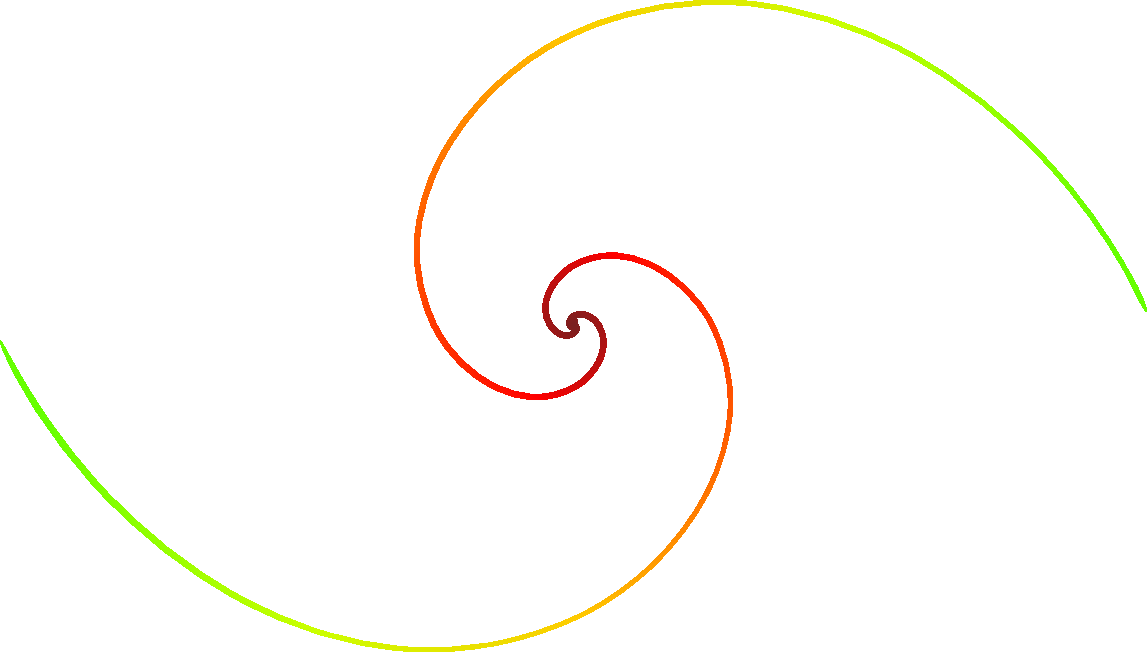
\includegraphics[scale=.5]{./pictures/curvature_color.pdf}\\

Zmiana koloru w zależności od krzywizny
\end{center}
\end{frame}
%%%%%%next-slide%%%%%
\begin{frame}{Krzywizna dowolnej krzywej}

Dla regularnych krzywych nieunormowanych możemy posłużyć się odpowiednią reparametryzacją:
\pause \begin{definicja}
Niech $\alpha\colon (a,b)\to \R^3$ będzie krzywą regularną, oraz niech $\beta=\alpha\circ h \colon (c,d)\to \R^3$ będzie jej reparametryzacją unormowaną ($h\colon (c,d)\to (a,b)$). Wówczas \[\kappa_\alpha(t)\define\kappa_\beta(h^{-1} (t)\!)\]
\end{definicja}

\pause\mode<presentation>{Czy definicja jest niezależna od wyboru parametryzacji?}

\end{frame}
%%%%%%next-slide%%%%%
Taka definicja rodzi natychmiast pytanie o jednoznaczność definicji krzywizny, ponieważ potencjalnie różne reparametryzacje unormowane mogą prowadzić do różnych funkcji krzywizny. Mamy jednak następujący lemat.

\begin{frame}[<+->]
\begin{lemat}
Niech $\alpha\colon(a,b)\to \R^3$ będzie krzywą regularną i niech $\alpha\circ h_1$ oraz $\alpha\circ h_2$ będą dwiema reparametryzacjami unormowanymi, gdzie $h_1\colon (c_1,d_1)\to (a,b)$, oraz $h_2\colon (c_2,d_2)\to (a,b)$ są dyfeomorfizmami. Jeśli $\kappa_1$ i $\kappa_2$ oznaczają krzywizny krzywych odpowiednio $\alpha\circ h_1$ oraz $\alpha\circ h_2$, wtedy\[\kappa_1(h_1^{-1}(t))=\kappa_2(h_2^{-1}(t))\]
dla wszystkich $t\in (a,b)$.

\end{lemat}

\begin{wniosek}
Definicja krzywizny dla krzywej nieunormowanej nie zależy od wyboru parametryzacji.
\end{wniosek}

\end{frame}
%%%%%%next-slide%%%%%
\begin{frame}[<+->]

\textcolor{ared}{\textbf{Dowód:}}\pause \\
Najpierw pokażemy, że $h_1$ i $h_2$ (funkcje reparametryzujące do krzywych unormowanych) mogą się różnić jedynie znakiem i przesunięciem, \pause tj. pokażemy, że złożenie \[h_2^{-1}\circ h_1\colon (c_1,d_1)\to (c_2,d_2)\] jest równe \[\left(h_2^{-1}\circ h_1\right)(t)=\pm t+C,\] dla pewnej stałej $C\in \R$.

\pause Dla obu indeksów $i=1,2$ i wszystkich $t\in (c_i,d_i)$ mamy 
\[1=\|(\alpha\circ h_i)'(t)\|=\|\alpha'(h_i(t))\||h'_i(t)|.\]
\end{frame}
%%%%%%next-slide%%%%%
\begin{frame}[<+->]

Zatem dla wszystkich $t\in (c_1,d_1)$ zachodzi 
\mode<article>{
\begin{multline*}
h_1'(t)=\frac{\pm1}{\|\alpha'(h_1(t))\|}=
\frac{\pm1}{\left\|\alpha'\left(h_2\left(h_2^{-1}\left[h_1(t)\right]
\right)\right)\right\|}=\pause\pm 
h_2\left[\left(h_2^{-1}\circ 
h_1\right)\!(t)\right]\!\!.
\end{multline*}}
\mode<presentation>{
\begin{multline*}
h_1'(t)=\frac{\pm1}{\|\alpha'(h_1(t))\|}=
\frac{\pm1}{\left\|\alpha'\left(h_2\left(h_2^{-1}\left[h_1(t)\right]
\right)\right)\right\|}=\\\pause=\pm 
h_2\left[\left(h_2^{-1}\circ 
h_1\right)\!(t)\right]\!\!.
\end{multline*}}

\pause Możemy teraz policzyć pochodną funkcji wewnętrznej:
\[
(h_2^{-1}\circ h_1)'(t)=\left(h_2^{-1}\right)'\big[h_1(t)\big]h_1'(t)=\frac{h_1'(t)}{h_2'(h_2^{-1}\circ h_1(t))}=\pm 1
\]

\pause Całkując obie strony równości otrzymujemy
\begin{align*}
\onslide<4->{\left(h_2^{-1}\circ h_1\right)(t)=}&\onslide<4->{\pm t+C\\}
\onslide<5->{h_1(t)=}&\onslide<5->{h_2(\pm t+C)\\}
\onslide<6->{h_2^{-1}(t)=}&\onslide<6->{h_1^{-1}(\pm t)+C.}
\end{align*}
\end{frame}
%%%%%%next-slide%%%%%
\begin{frame}[<+->]


Podstawiając przedostatnią równość do $\alpha$ mamy 
\[(\alpha\circ h_1)(t)=(\alpha\circ h_2)(\pm t+C),\]
\pause więc zachodzi również $\kappa_1(t)=\kappa_2(\pm t+C)$. \pause Podstawiając teraz $t=h_1^{-1}(s)$ otrzymujemy 
\[\kappa_1(h_1^{-1})(s)=\kappa_2(h_1^{-1}(s)+C)=\kappa_2(h_2^{-1}(s)\!).\]
\hfill $\square$

\end{frame}
%%%%%%next-slide%%%%%

\begin{uwaga}
Na razie pokazaliśmy, że dla \textit{wybranej} parametryzacji $\alpha$ krzywizna 
nie zależy od reparametryzacji unormowanej.

Chcemy jednak pokazać coś więcej, mianowicie, że krzywizna jest funkcją zależną tylko od \textit{punktów w obrazie krzywej} i w ogóle nie zależy od wyboru \textit{parametryzacji}. Zostanie to wykazane pod koniec tego wykładu.
\end{uwaga}


%%%%%%next-slide%%%%%
\begin{frame}

\begin{lemat}
Niech $\alpha\colon (a,b)\to \R^3$ będzie krzywą regularną. Wektor normalny do $\alpha$ jest zerowy wtedy i tylko wtedy, gdy $\alpha$ jest prostą.
\end{lemat}
\pause\textcolor{ared}{\textbf{Dowód:}}\\
Bez straty ogólności możemy założyć, że $\alpha$ jest krzywą unormowaną.
\pause Załóżmy, że wektor normalny do $\alpha$ jest zerowy, \[\frac{T'(t)}{|T'(t)|}=N(t)=(0,0,0).\] \pause 
Całkując to równanie otrzymujemy 
 \begin{multline*}
T(t)=\int T'(t)\,dt=\left(\int T_1 '(t)\,dt,\int T_2 '(t)\,dt, \int T_3 '(t)\,dt\right)=\pause\\=\left(\int 0\,dt,\int 0\,dt, \int 0\,dt\right)=(c_1,c_2,c_3)=v=\text{\footnotesize{const}}.
\end{multline*}


\end{frame}
%%%%%%next-slide%%%%%
\begin{frame}[<+->]
Całkując ponownie mamy \[\alpha(t)=vt+w,\] gdzie $v,w\in \R^3$ są ustalonymi wektorami, czyli $\alpha$ jest prostą.
\pause 
Załóżmy teraz, że $\alpha$ jest prostą. \pause Mamy wtedy (postać parametryczna prostej) $\alpha(t)=vt+w$, gdzie $v,w\in \R^3$. \pause Wtedy oczywiście \[T(t)=\frac{\alpha'(t)}{\|\alpha'(t)\|}=\frac{v}{\|v\|},\] zatem $T\,'(t)=0$ więc automatycznie $N(t)=0$.
\hfill $\square$

\end{frame}
%%%%%%next-slide%%%%%
\mode<all>{\midsection{Torsja}}
\begin{frame}
\begin{definicja}
Niech $\alpha\colon (a,b)\to \R^3$ będzie krzywą regularną, oraz załóżmy, że dla wszystkich $t\in (a,b)$ zachodzi $N(t)\neq 0$. \textbf{Torsję} krzywej $\alpha$ w punkcie $t$ definiujemy jako funkcję \[\tau(t)\define \langle B'(t),N(t)\rangle.\]
\end{definicja}
\pause
\begin{uwaga}
\begin{itemize}
\item Torsja jest funkcją gładką (wynika to z gładkości iloczynu skalarnego).
\pause\item Podobnie jak w przypadku krzywizny mamy $|\tau(t)|=\|B'(t)\|$, 
jednak torsja może mieć wartości \textit{ujemne}.
\end{itemize}
\end{uwaga}

\end{frame}
%%%%%%next-slide%%%%%
\begin{frame}[<+->]

\begin{uwaga}
Dla wygody od teraz będziemy opuszczać argument $t$ jeśli nie będzie to prowadziło do niejednoznaczności.
\end{uwaga}

\end{frame}
%%%%%%next-slide%%%%%
\mode<all>{\midsection{Wzory Freneta}}
\begin{frame}
\begin{twierdzenie}[Wzory Freneta] Niech $\alpha\colon (a,b)\to \R^3$ będzie unormowaną krzywą regularną, r\'ożną od stałej i prostej (tj. $N(t)\neq 0$ dla wszystkich $t\in (a,b)$). Wówczas zachodzą następujące równości.
\begin{align}
T\,'	&= \qquad\kappa N \label{eqn:frenet1} \\
N\hspace{0.5pt}'	&= -\kappa T + \tau B\label{eqn:frenet2}\\
B'	&= \quad-\tau N\label{eqn:frenet3}
\end{align}
\pause co można zapisać w postaci wektorowej
\[
\left(\begin{array}{c}
 T\\
 N\\
 B
 \end{array}\right)'=
 \left[\begin{array}{r r r}
 0 & \kappa & 0\\
 -\kappa & 0 & \tau\\
 0 & -\tau &0
 \end{array}\right]
 \left(\begin{array}{c}
  T\\
 N\\
 B
 \end{array}\right)
\]


\end{twierdzenie}

\end{frame}
%%%%%%next-slide%%%%%
\begin{frame}

\textcolor{ared}{\textbf{Dowód:}}\pause \\
Wzór \ref{eqn:frenet1} na $T\,'$ wynika z przyjętych definicji $\kappa$ i $N$.

\pause Ponieważ wektory z repera Freneta są jednostkowe, więc $N\hspace{0.5pt}'$ jest prostopadły do $N$. Ponieważ jednak ${T,N,B}$ tworzy bazę przestrzeni $\R^3$, więc $N\hspace{0.5pt}'$ musi być kombinacją liniową wektorów $T$ i $B$,\[N\hspace{0.5pt}'=a T+b B.\] 
\pause Mnożąc tę równość skalarnie przez wektor $T$ (odpowiednio $B$) otrzymujemy $a=\langle N\hspace{0.5pt}',T\hspace{0.5pt}\rangle$ (odpowiednio $b=\langle N\hspace{0.5pt}',B\rangle$). \pause Wyliczenie $a$ rozpocznijmy od równości $0=\langle N,T\hspace{0.5pt}\rangle$. Różniczkując obie strony otrzymujemy
\pause \[0=\langle N\hspace{0.5pt}',T\hspace{0.5pt}\rangle+\langle N,T\,'\rangle=\langle N\hspace{0.5pt}',T\hspace{0.5pt}\rangle+\underbrace{\langle N,\kappa N\rangle}_{=\kappa},\]
\pause zatem $a=\langle N\hspace{0.5pt}',T\hspace{0.5pt}\rangle=-\kappa$. \pause Ponieważ $\langle N,B\rangle=0$, w podobny sposób możemy stwierdzić, że $\langle N\hspace{0.5pt}',B\rangle=-\tau$. Pozostawiamy to jako zadanie domowe.

\end{frame}
%%%%%%next-slide%%%%%
\begin{frame}[<+->]
Podobnie $B'$ jest prostopadły do $B$, $\langle B,B'\rangle=0$, więc
\[B'=a T+b N.\]
\pause Musimy więc policzyć $a=\langle B',T\hspace{0.5pt}\rangle$ i $b=\langle B',N\rangle$. Wyliczenie $a$ rozpocznijmy od równości: $0=\langle B,T\hspace{0.5pt}\rangle$. \pause Różniczkując obie strony otrzymujemy
\[0=\langle B',T\hspace{0.5pt}\rangle+\langle B,T\,'\rangle=\langle B',T\hspace{0.5pt}\rangle+\langle B,\kappa N\rangle=\langle B',T\hspace{0.5pt}\rangle.\]
\pause Tak więc $B'$ jest współliniowy z $N$ i równość \ref{eqn:frenet3} charakteryzująca $B'$ wynika z definicji torsji $\tau$.

\hfill $\square$

\end{frame}
%%%%%%next-slide%%%%%
\begin{frame}[<+->]

\begin{lemat}
Niech $\alpha\colon (a,b)\to \R^3$ będzie krzywą unormowaną oraz niech $N(t)\neq 0$ dla każdego $t\in (a,b)$. Następujące warunki są równoważne.
\begin{enumerate}
\item Zbi\'or $\alpha(a,b)$ (tj. wykres $\alpha$) jest zawarty w pewnej płaszczyźnie.
\item $B$ jest wektorem stałym.
\item $\tau\equiv 0$.
\end{enumerate}

\end{lemat}

\begin{uwaga}
Krzywą spełniającą jeden z tych warunków nazywamy \textbf{krzywą płaską}.
\end{uwaga}

\end{frame}
%%%%%%next-slide%%%%%
\begin{frame}

\textcolor{ared}{\textbf{Dowód:}}\pause \\
\begin{description}
\item [$1\Rightarrow 2$] Jeśli krzywa leży w jednej płaszczyźnie to leżą w niej 
wektory styczny i normalny (dlaczego?), \pause więc jest to płaszczyzna ściśle 
styczna. \pause Wtedy kierunek prostopadły do tej płaszczyzny jest współliniowy 
z $B$. Zatem $B$ nie zmienia ani zwrotu ani długości.\pause
\item [$2\Leftrightarrow 3$] wynika ze wzoru Freneta (\ref{eqn:frenet3}):
\[B'=-\tau N\]
\end{description}

\end{frame}
%%%%%%next-slide%%%%%
\begin{frame}
\begin{description}
\item [$2\Rightarrow 1$] Niech $p\in (a,b)$ będzie punktem z dziedziny $\alpha$. 
\mode<presentation>{\begin{itemize}}
\mode<presentation>{\pause\item}
Rozważmy funkcję
\[f(t)=\langle \alpha(t)-\alpha(p),B(t)\rangle.\]

\mode<article>{
Funkcja ta mierzy długość rzutu wektora binormalnego na wektor wyznaczony przez naszą krzywą (bez straty ogólności możemy założyć, że $\alpha(p)=(0,0,0)$.)}

\mode<presentation>{\pause\item}
Przy założeniu, że $B(t)=B$ jest wektorem stałym, pokażemy, że funkcja $f$ jest tożsamościowo równa $0$, \pause z czego wynika, że krzywa $\alpha$ w całości leży w płaszczyźnie normalnej do $B$ i zawierającej punkt $\alpha(p)$.
\mode<presentation>{\end{itemize}}
\end{description}
\end{frame}
%%%%%%next-slide%%%%%
\begin{frame}
\mode<presentation>{\begin{itemize}}
\mode<presentation>{\item}
Obliczmy 
\[\begin{split}
f\,'(t)=&\pause\frac{d}{dt}\left(\langle\alpha(t)-\alpha(p),B(t)\rangle\right)=\\
\uncover<3->{=}&\uncover<3->{\underbrace{\langle\alpha'(t),B(t)\rangle}_{=\langle T(t),B(t)\rangle=0}+}
\uncover<4->{\underbrace{\langle\alpha(t)-\alpha(p),B'(t) \rangle}_{=0\text{ bo $B(t)$ jest stały}}=0.}
\end{split}\]
\uncover<5->{
\mode<presentation>{\item} Zatem $f$ jest funkcją stałą. Jeśli podstawimy $t=p$ otrzymamy $f(p)=0$, więc $f$ jest tożsamościowo równa $0$.}
\mode<presentation>{\end{itemize}}

\hfill $\square$
\end{frame}
%%%%%%next-slide%%%%%
\mode<all>{\midsection{Wzory ogólne}}
\begin{frame}
\begin{lemat}[Wzory og\'olne]\label{lem_curv:wzory-ogolne}
Niech $\alpha\colon (a,b)\to \R^3$ będzie krzywą regularną r\'ożną od prostej (tj. $N(t)\neq 0$ dla każdego $t\in (a,b)$). Wówczas zachodzą następujące wzory:
\begin{align}
\pause T=& \frac{\alpha'}{\|\alpha'\|}\label{eqn:T}\\
\pause B=& \frac{\alpha'\times \alpha''}{\|\alpha'\times \alpha''\|}\label{eqn:B}\\
\pause N=& B\times T\label{eqn:N}\\
\pause \kappa=&\frac{\|\alpha'\times \alpha''\|}{\|\alpha'\|^3}\label{eqn:k}\\
\pause \tau=&\frac{\langle \alpha'\times \alpha'',\alpha'''\rangle}{\|\alpha'\times \alpha''\|}\label{eqn:t}
\end{align}

\end{lemat}
\end{frame}
%%%%%%next-slide%%%%%
\begin{frame}

\textcolor{ared}{\textbf{Dowód:}}\pause \\
Dowód  polega na przeliczeniu odpowiednich pochodnych bez zakładania, że $\alpha$ jest krzywą unormowaną. Pozostawiamy go jako ćwiczenie.
\hfill $\square$

\pause\begin{uwaga}
Powyższy lemat pozwala liczyć trójnóg Freneta, krzywiznę i torsję nie odwołując się do \textit{żadnej unormowanej parametryzacji}. Dowodzi to, że $T,N,B,\kappa$ i $\tau$ są funkcjami tylko i wyłącznie punktów na krzywej (rozumianej jako obraz wykresu w $\R^3$) i nie zależą od parametryzacji.
\end{uwaga}

\end{frame}
\mode<all> 

\mode*
\mode<all>{\topsection{Twierdzenie klasyfikacyjne dla krzywych}}
\mode<all>{\midsection{Translacja i obrót}}
\begin{frame}[<+->]
\begin{lemat}
Niech $\alpha\colon (a,b)\to \R^3$ będzie krzywą regularną. 
\begin{itemize}
\item Translacja krzywej $\alpha$, tj. krzywa $\beta=\alpha+q$, gdzie $q\in \R^3$ jest wybranym \textit{stałym} wektorem ma taką samą krzywiznę i torsję jak $\alpha$.
\item Niech $A\in O(3)$ będzie macierzą $3\times 3$ o współczynnikach 
rzeczywistych, o wyznaczniku $\pm1$ oraz ortnormalnych kolumnach. Krzywa 
\[\gamma\define A\cdot\alpha\] ma taką samą krzywiznę i torsję jak $\alpha$.
\end{itemize}
\end{lemat}

\begin{uwaga}
Dowód pierwszej części jest bardzo prosty. Dowód drugiej pozostawiamy jako bardziej ambitne zadanie.
\end{uwaga}

\end{frame}
%%%%%%next-slide%%%%%
\begin{frame}[<+->]

Mnożenie przez taką macierz $A$ oznacza obrót wokół środka układu współrzędnych, symetrię względem płaszczyzny, lub kombinację tych dwóch. Grupa $O(3)$ to tzw. grupa symetrii $\R^3$ i jej bazę stanowią macierze obrotów o dowolny kąt wokół każdej z osi, oraz macierz symetrii względem (dowolnie wybranej) płaszczyzny zawierającej punkt $(0,0,0)$.

\end{frame}
%%%%%%next-slide%%%%%
\begin{uwaga}
Grupa składająca się ze wszystkich obrotów oraz translacji przestrzeni 
euklidesowej $\R^3$ jest tzw. \textit{grupą Liego} $E(3)$. Jest to grupa 
izometrii (poznamy to pojęcie w następnej części wykładu) przestrzeni 
euklidesowej . Intuicyjnie mamy trzy ``stopnie swobody'' pochodzące od obrotu i 
kolejne trzy od translacji o wektor, więc grupa $E(3)$ powinna być 
,,$6$-wymiarowa''. 
\end{uwaga}


\begin{frame}[<+->]

\begin{uwaga}
Te dwie operacje definiują nam relację równoważności pomiędzy wykresami krzywych w $\R^3$. Krzywą $\alpha$ uznajemy za równoważną krzywej $\beta$, jeśli wykres $\beta$ można otrzymać przez zastosowanie odpowiednich translacji, obrotów i symetrii do wykresu $\alpha$.
\end{uwaga}

\end{frame}
%%%%%%next-slide%%%%%
\mode<all>{\midsection{Twierdzenie klasyfikacyjne}}
\begin{frame}[<+->]
\begin{twierdzenie}[Klasyfikacyjne]
Niech $\kappa, \tau\colon (a,b)\to \R$ będą gładkimi funkcjami, oraz niech $\kappa(t)>0$ dla wszystkich $t\in (a,b)$. Wówczas zachodzą następujące stwierdzenia.
\begin{itemize}
\item Istnieje taka krzywa gładka \[\alpha\colon(a,b)\to\R^3,\] że jej krzywizna $\kappa_\alpha$ i torsja $\tau_\alpha$ są tożsamościowo równe funkcjom $\kappa$ oraz $\tau$. 
\item Jeśli \[\beta\colon (a,b)\to \R^3\] jest drugą taką krzywą, to krzywą $\beta$ można uzyskać z $\alpha$ stosując przesunięcia obroty i symetrie w przestrzeni $\R^3$.
\end{itemize}

\end{twierdzenie}

\end{frame}
%%%%%%next-slide%%%%%
\begin{frame}[<+->]

\textcolor{ared}{Szkic dowodu:}\pause\\
Niech $p\in (a,b)$. Pokażemy, że istnieje dokładnie jedyna krzywa unormowana $\alpha\colon(a,b)\to \R^3$ taka, że 
\pause\begin{align*}
&&\alpha(p)&=
\left(\!\!\begin{array}{c}
0\\0\\0
\end{array}\!\!\right)\!,&\text{oraz}\\
T_\alpha(p)&=\left(\!\!\begin{array}{c}
1\\0\\0
\end{array}\!\!\right)\!,& 
N_\alpha(p)&=\left(\!\!\begin{array}{c}
0\\1\\0
\end{array}\!\!\right)\!,& 
B_\alpha(p)&=\left(\!\!\begin{array}{c}
0\\0\\1
\end{array}\!\!\right)
\label{eqn:warunek_poczatkowy}
\end{align*}
o zadanej krzywiźnie i torsji (dlaczego to wystarczy?).

\end{frame}
%%%%%%next-slide%%%%%
Szukamy zatem dziewięciu funkcji $u_1(t),\ldots,u_9(t)$ które będą tworzyć wektory $T_\alpha(t)$, $N_\alpha(t)$ i $B_\alpha(t)$ dla domniemanej krzywej $\alpha$. Oczywiście jeśli taka krzywa ma w ogóle istnieć, funkcje te muszą spełniać odpowiednie równania, wynikające ze wzorów Freneta. Poniższy układ jest konsekwencją dokładnie tego faktu.

\begin{frame}[<+->]

\mode<presentation>{Dowód polega na rozwiązaniu następującego układu równań różniczkowych zadanego przez równania Freneta wraz z warunkiem początkowym zadanym powyżej:}

% \begin{align*}
% \left(\!\!\begin{array}{c}
% u_1\\u_2\\u_3
% \end{array}\!\!\right)\!(p)
% &=
% \left(\!\!\begin{array}{c}
% 1\\0\\0
% \end{array}\!\!\right)\!,
% &
% \left(\!\!\begin{array}{c}
% u_4\\u_5\\u_6
% \end{array}\!\!\right)\!(p)
% &=
% \left(\!\!\begin{array}{c}
% 0\\1\\0
% \end{array}\!\!\right)\!,
% &
% \left(\!\!\begin{array}{c}
% u_7\\u_8\\u_9
% \end{array}\!\!\right)\!(p)
% &=
% \left(\!\!\begin{array}{c}
% 0\\0\\1
% \end{array}\!\!\right)\!,
% \end{align*}
\vspace*{-0.2in}
\begin{align*}
\pause\left.\begin{aligned}      
u_1'(t)&=\kappa(t)u_4(t)\\
u_2'(t)&=\kappa(t)u_5(t)\\
u_3'(t)&=\kappa(t)u_6(t)
\end{aligned}\right\}&\;\text{dla }``T\,'=\kappa N\text{''}\!,\quad\\
\pause\left.\begin{aligned}      
u_7'(t)&=\tau(t)u_4(t)\\
u_8'(t)&=\tau(t)u_5(t)\\
u_9'(t)&=\tau(t)u_6(t)
\end{aligned}\right\}&\;\text{dla }``B'=-\tau N\text{''}\!,
\end{align*}
\vspace*{-0.1in}
\pause\begin{equation*}
\left.\begin{aligned}      
u_4'(t)&=-\kappa(t)u_1(t)+\tau(t)u_7(t)\\
u_5'(t)&=-\kappa(t)u_2(t)+\tau(t)u_8(t)\\
u_6'(t)&=-\kappa(t)u_3(t)+\tau(t)u_9(t)
\end{aligned}\right\}\;\text{dla }``N\hspace{0.5pt}'=-\kappa T+\tau B\text{''}.
\end{equation*}
\vspace*{-0.2in}
\pause \begin{align*}
u_1(p)&=1 & u_4(p)&=0 & u_7(p)&=0\\ 
u_2(p)&=0 & u_5(p)&=1 & u_8(p)&=0\\
u_3(p)&=0 & u_6(p)&=0 & u_9(p)&=1\\ 
 \end{align*}

\end{frame}
%%%%%%next-slide%%%%%
\begin{frame}[<+->]
\begin{twierdzenie}[Picarda, o istnieniu i jedyności rozwiązania równania różniczkowego]\label{thm:dif-eq-solution}
Niech $(a,b)\subset \R$, oraz  niech $A\in M_{n,n}(\R)$.  Ustalmy liczbę $t_0\in 
(a,b)$ i punkt $v_0\in \R^n$. Wtedy istnieje dokładnie jedna funkcja gładka 
$\omega\colon (a,b)\to \R^n$ która spełnia 
\begin{align*}
\omega(t_0)&=v_0,\quad\text{oraz}\\
\omega'(t)&=A\omega(t) \quad\text{dla wszystkich }t\in (a,b).
\end{align*}
\end{twierdzenie}

\begin{exercise}
Przepisać sformułowanie naszego problemu tak, aby zastosować do niego powyższe 
twierdzenie \\(podać $\omega$, $A$, $t_0$ i $v_0$). 
\end{exercise}

\end{frame}
%%%%%%next-slide%%%%%
\begin{frame}[<+->]
Na mocy powyższego twierdzenia istnieją więc trzy wektory (albo $9$ funkcji) 
\begin{align*}
\pause X_1(t)&=\left(\!\!\begin{array}{c}
u_1\\u_2\\u_3
\end{array}\!\!\right)\!(t),&
\pause X_2(t)&=\left(\!\!\begin{array}{c}
u_4\\u_5\\u_6
\end{array}\!\!\right)\!(t),&
\pause X_3(t)&=\left(\!\!\begin{array}{c}
u_7\\u_8\\u_9
\end{array}\!\!\right)\!(t).
\end{align*}
spełniające nasz układ wraz z warunkiem początkowym. \pause Możemy myśleć o nich jako o $\{T,N,B\}$ dla krzywej która realizuje $\kappa$ jako krzywiznę i $\tau$ jako torsję.

\pause Aby pokazać, że $\{X_1(t),X_2(t),X_3(t)\}$ tworzą bazę ortogonalną dla wszystkich $t\in (a,b)$ posłużymy się następującą funkcją: \[p_{i,j}(t)=\langle X_i(t),X_j(t)\rangle, \qquad i,j=1,2,3.\]

\pause Oczywiście mamy (warunek początkowy na $X_1$, $X_2$ i $X_3$)
\begin{equation}\label{eqn:initial-cond}
p_{i,j}(p)=
\begin{cases}
1 & i=j\\
0 & i\neq j\\
\end{cases}
\end{equation}
\end{frame}
%%%%%%next-slide%%%%%
\begin{frame}[<+->]
\begin{exercise}
Sformułować układ równań wiążących pochodne funkcji $p'_{i,j}(t)$ z funkcjami $\{p_{i,j}(t)\}$ oraz $\kappa(t)$ i $\tau(t)$.
\end{exercise}

\begin{przyklad}\mode<presentation>{\vspace*{-0.25in}}
\[\begin{split}
p_{1,1}'(t)=&\left(\langle X_1(t),X_1(t)\rangle\right)'=\\
=&\underbrace{\langle X_1'(t)}_{=\kappa(t)X_2(t)},X_1(t)\rangle+\langle X_1(t),\underbrace{X_1'(t)\rangle}_{=\kappa(t) X_2(t)}=\\=&\kappa(t) p_{2,1}(t)+\kappa(t)p_{1,2}(t).
\end{split}
\]
\end{przyklad}

\end{frame}
%%%%%%next-slide%%%%%
\begin{frame}[<+->]
Uzyskany układ wraz z warunkami początkowymi (\ref{eqn:initial-cond}) ponownie posiada \textit{jednoznaczne} rozwiązanie na mocy twierdzenia cytowanego powyżej. \pause Można sprawdzić, że delta Kroneckera 
\[\delta_{ij}(t)=\begin{cases}
            1,&i=j\\
	0, & i\neq j
            \end{cases}\]
spełnia otrzymany układ, a zatem jest jedynym rozwiązaniem. \pause Z definicji $p_{i,j}(t)$ wynika, że $\{X_1(t),X_2(t),X_3(t)\}$ tworzy bazę ortogonalną dla wszystkich $t$.

\pause Możemy wreszcie zdefiniować 
\[\alpha(t)\define\int_p^t X_1(s)\;ds.\]

\end{frame}
%%%%%%next-slide%%%%%
\begin{frame}[<+->]

Łatwo można sprawdzić, że dla tak zdefiniowanej krzywej zachodzą równości
\begin{align*}
\pause \alpha'(t)=T_\alpha(t)& =X_1(t)\\
\pause \alpha''(t)=\kappa_\alpha(t)N_\alpha(t)&=\kappa(t) X_2(t)\\
\pause |\tau_\alpha(t)|B_\alpha(t)&=\tau(t) X_3(t).
\end{align*}

\pause Pozostaje jedynie pokazać, że zgadzają się zwroty wektorów $X_3(t)$ i $B_\alpha(t)$. 

\footnotesize
\pause Jest to ładny argument wykorzystujący niezdegenerowanie naszego trójnogu, oraz to, że w jednym punkcie (czyli w $p$) ten zwrot jest taki sam. Zostawiamy to jako zadanie domowe.

\normalsize
\hfill $\square$
\end{frame}
%%%%%%next-slide%%%%%
% \begin{frame}[<+->]
% 
% \midsection{Przykład:}
% 
% @@@Uzupełnić@@@

\mode<all> 


%%%		6 wykładów o krzywiźnie powierzchni			%
 \setcounter{section}{4}
 \mode*
\mode<all>{\topsection{Powierzchnie w $\R^3$}}

\begin{frame}[<+->]
\begin{definicja}
Niech $U\subset\R^2$ będzie zbiorem otwartym. Odwzorowanie (funkcję wektorową) \[x\colon U\to \R^3\] nazywamy \textbf{gładkim}, jeśli wszystkie pochodne cząstkowe (dowolnego rzędu) $x$ istnieją oraz są odwzorowaniami ciągłymi.
\end{definicja}

\begin{definicja}
Niech $U\subset \R^2$ będzie zbiorem otwartym. Odwzorowanie gładkie
\[x\colon U\to \R^3\]
nazywamy \textbf{lokalnym układem współrzędnych} jeśli jest injekcją, oraz \[\frac{\partial x}{\partial s}(s,t)\times \frac{\partial x}{\partial t}(s,t)\neq 0\] dla wszystkich $(s,t)\in U$.
\end{definicja}

\end{frame}
%%%%%%next-slide%%%%%
\mode<all>{\midsection{Podstawowe definicje}}
\begin{frame}[<+->]

\begin{definicja}\label{def:surface}
\begin{itemize}
\item 
Podzbiór $M\subset \R^3$ nazywamy \textbf{powierzchnią gładką}, jeśli wokół każdego punktu $p$ istnieje lokalny układ współrzędnych $x\colon U\to V\subset \R^3$. 

%\item Powierzchnię gładką $M$ nazywamy \textbf{regularną}  

\item Powierzchnię gładką $M$ nazywamy łukowo spójną, jeśli dla dowolnych dwóch punktów $x,y\in M$ istnieje krzywa $\alpha\colon [0,1]\to M$ taka, że $\alpha(0)=x$ i $\alpha(1)=y$.
\end{itemize}
\end{definicja}

\pause Potocznie mówimy, że przestrzeń jest powierzchnią gładką jeśli ,,lokalnie'' (tj. w małym otoczeniu każdego punktu) wygląda jak fragment płaszczyzny (patrz część 1 Lematu \ref{lem:chart_loc_bij}).


\end{frame}
%%%%%%next-slide%%%%%
\begin{frame}[<+->]

\begin{przyklad}
Jednostkowa sfera, tj. powierzchnia o równaniu $x^2+y^2+x^2=1$ jest przykładem powierzchni regularnej. Lokalnym układem współrzędnych jest np. $x^\pm(u,v)=(\pm\sqrt{1-u^2-v^2},u,v)$ jak na następującym rysunku

\begin{center}
%\begin{tikzpicture}[y=0.80pt, x=0.8pt,scale=0.25,yscale=-1, inner sep=0pt, outer sep=0pt]
\usetikzlibrary{arrows}
\mode<presentation>{\begin{tikzpicture}[y=0.80pt, x=0.8pt,scale=0.3,yscale=-1, inner sep=0pt, outer sep=0pt]}
\mode<article>{\begin{tikzpicture}[y=0.80pt, x=0.8pt,scale=0.4,yscale=-1, inner sep=0pt, outer sep=0pt]}
\begin{scope}[shift={(-22.88722,-49.76189)}]% layer1
  \begin{scope}[shift={(-739.46591,328.36782)}]% g1515
    % path53
    \path[fill=black] (814.4212,58.5435) .. controls (820.3754,93.7311) and
      (836.8215,127.0965) .. (861.8065,152.5185) .. controls (861.8065,152.5185) and
      (861.8065,152.5185) .. (861.8065,152.5185) .. controls (877.3745,168.3508) and
      (896.0728,181.0812) .. (916.5208,189.7208) .. controls (916.5208,189.7208) and
      (916.5208,189.7208) .. (916.5208,189.7208) .. controls (938.2006,198.8777) and
      (961.7638,203.3783) .. (985.2680,203.2928) .. controls (985.2680,203.2928) and
      (985.2680,203.2928) .. (985.2680,203.2928) .. controls (988.4665,203.2814) and
      (991.6647,203.1752) .. (994.8567,202.9746) .. controls (1015.0320,201.7064)
      and (1034.9702,196.7427) .. (1053.2767,188.1710) .. controls
      (1073.3535,178.7669) and (1091.3975,165.1492) .. (1106.2074,148.6496) ..
      controls (1106.2074,148.6496) and (1106.2074,148.6496) .. (1106.2074,148.6496)
      .. controls (1120.8905,132.2919) and (1132.4412,113.1366) ..
      (1140.1348,92.5338) .. controls (1147.1845,73.6587) and (1150.9849,53.5407) ..
      (1151.0552,33.3886) .. controls (1151.0652,31.5089) and (1151.0372,29.6289) ..
      (1150.9802,27.7496) .. controls (1150.9802,27.7496) and (1150.9802,27.7496) ..
      (1150.9802,27.7496) .. controls (1150.3459,6.7970) and (1145.7929,-14.0185) ..
      (1137.7201,-33.3655) .. controls (1129.6473,-52.7126) and (1118.0511,-70.5899)
      .. (1103.3264,-85.6015) .. controls (1103.3264,-85.6015) and
      (1103.3263,-85.6015) .. (1103.3263,-85.6015) .. controls (1088.9567,-100.2437)
      and (1071.7700,-112.1497) .. (1052.9265,-120.3583) .. controls
      (1052.9265,-120.3583) and (1052.9264,-120.3583) .. (1052.9264,-120.3583) ..
      controls (1034.2127,-128.5074) and (1013.9178,-132.9553) ..
      (993.5271,-133.5322) .. controls (992.5638,-133.5595) and (991.6002,-133.5783)
      .. (990.6366,-133.5886) .. controls (968.3513,-133.8241) and
      (946.1243,-129.4717) .. (925.4123,-121.4288) .. controls (904.6002,-113.3501)
      and (885.2493,-101.5604) .. (868.6019,-86.7416) .. controls
      (868.6019,-86.7416) and (868.6019,-86.7416) .. (868.6019,-86.7416) .. controls
      (852.0572,-72.0170) and (838.1847,-54.2239) .. (828.5521,-34.3115) .. controls
      (828.5521,-34.3115) and (828.5521,-34.3115) .. (828.5521,-34.3115) .. controls
      (821.1762,-19.0603) and (816.3964,-2.5704) .. (814.5363,14.2211) .. controls
      (813.5712,19.9703) and (813.4850,24.2752) .. (813.6871,27.0631) .. controls
      (813.8891,29.8509) and (814.3785,31.1348) .. (814.8395,30.9987) .. controls
      (815.3006,30.8625) and (815.7362,29.3143) .. (816.0857,26.4386) .. controls
      (816.4352,23.5630) and (816.7007,19.3626) .. (817.0351,13.8445) .. controls
      (818.9464,-2.4347) and (823.6513,-18.4133) .. (830.8336,-33.1926) .. controls
      (830.8336,-33.1926) and (830.8336,-33.1926) .. (830.8336,-33.1926) .. controls
      (840.3409,-52.7626) and (854.0447,-70.2570) .. (870.3712,-84.7362) .. controls
      (870.3712,-84.7362) and (870.3712,-84.7362) .. (870.3712,-84.7362) .. controls
      (886.8048,-99.3078) and (905.9029,-110.8894) .. (926.4191,-118.8074) ..
      controls (946.8363,-126.6852) and (968.7161,-130.9288) .. (990.5966,-130.6503)
      .. controls (991.0043,-130.6453) and (991.4120,-130.6384) ..
      (991.8197,-130.6302) .. controls (1012.3883,-130.2142) and
      (1032.8870,-125.7854) .. (1051.7088,-117.5386) .. controls
      (1051.7088,-117.5386) and (1051.7088,-117.5386) .. (1051.7088,-117.5386) ..
      controls (1070.1704,-109.4514) and (1087.0055,-97.7342) ..
      (1101.0624,-83.3551) .. controls (1115.4667,-68.6278) and (1126.8038,-51.0718)
      .. (1134.6899,-32.0835) .. controls (1142.5760,-13.0952) and
      (1147.0149,7.3240) .. (1147.6166,27.8466) .. controls (1147.6166,27.8466) and
      (1147.6166,27.8466) .. (1147.6166,27.8466) .. controls (1147.6326,28.3811) and
      (1147.6456,28.9157) .. (1147.6556,29.4504) .. controls (1148.0610,50.0902) and
      (1144.4865,71.3087) .. (1137.0911,91.3998) .. controls (1129.6869,111.5099)
      and (1118.4636,130.5046) .. (1104.0814,146.7470) .. controls
      (1104.0814,146.7470) and (1104.0814,146.7470) .. (1104.0814,146.7470) ..
      controls (1089.5700,163.1345) and (1071.8025,176.6809) .. (1052.2415,185.9599)
      .. controls (1033.5864,194.8132) and (1013.3474,199.6927) ..
      (993.3781,200.7747) .. controls (990.6689,200.9215) and (987.9644,200.9976) ..
      (985.2676,201.0040) .. controls (961.5766,201.0586) and (938.4845,196.3434) ..
      (917.5424,187.3157) .. controls (897.3796,178.6265) and (879.2041,165.9873) ..
      (864.0382,150.3361) .. controls (853.1146,139.0685) and (843.8358,126.2066) ..
      (836.3499,112.1612) .. controls (828.8641,98.1157) and (823.1671,82.8815) ..
      (819.5655,66.8410) .. controls (818.7252,63.1879) and (817.7457,58.5408) ..
      (816.9211,53.7921) .. controls (816.0965,49.0434) and (815.4294,44.1954) ..
      (814.9282,40.1943) .. controls (814.4270,36.1933) and (814.0732,33.0404) ..
      (813.7050,31.7033) .. controls (813.5209,31.0348) and (813.3320,30.8205) ..
      (813.1355,31.1839) .. controls (812.9389,31.5473) and (812.7330,32.4884) ..
      (812.5534,34.1326) .. controls (812.4051,37.7311) and (812.5169,41.8343) ..
      (812.8565,46.0352) .. controls (813.1964,50.2361) and (813.7641,54.5330) ..
      (814.4212,58.5435) -- cycle;

    % path55
    \path[fill=black] (1018.1258,197.5435) .. controls (1032.1810,189.3284) and
      (1044.9190,178.8829) .. (1055.1265,166.2307) .. controls (1066.2029,152.4809)
      and (1074.1578,136.3667) .. (1078.9331,119.4360) .. controls
      (1078.9331,119.4360) and (1078.9331,119.4360) .. (1078.9331,119.4360) ..
      controls (1079.3917,117.8099) and (1079.8224,116.1770) .. (1080.2257,114.5379)
      .. controls (1083.8144,99.9537) and (1085.4669,84.9341) .. (1085.5968,69.9374)
      .. controls (1085.7286,54.9173) and (1084.3602,39.8820) .. (1081.5801,25.1175)
      .. controls (1081.5801,25.1175) and (1081.5801,25.1175) .. (1081.5801,25.1175)
      .. controls (1080.5850,19.8377) and (1079.3114,14.6203) .. (1077.7951,9.4756)
      .. controls (1074.5536,-1.5229) and (1070.4034,-12.2558) ..
      (1065.6350,-22.6709) .. controls (1065.6350,-22.6709) and (1065.6350,-22.6709)
      .. (1065.6350,-22.6709) .. controls (1057.3777,-40.7226) and
      (1046.9982,-57.9471) .. (1033.9537,-73.0247) .. controls (1031.2633,-76.1370)
      and (1028.4516,-79.1565) .. (1025.5200,-82.0570) .. controls
      (1013.8830,-93.5707) and (1000.5506,-103.4031) .. (985.6962,-110.2445) ..
      controls (985.6962,-110.2445) and (985.6962,-110.2445) .. (985.6962,-110.2445)
      .. controls (976.2165,-114.6053) and (966.1590,-117.6954) ..
      (955.8750,-119.2930) .. controls (947.1619,-120.6449) and (938.3137,-120.9197)
      .. (929.5634,-120.2180) .. controls (927.1037,-120.3482) and
      (925.3145,-120.0704) .. (924.1845,-119.6647) .. controls (923.0544,-119.2591)
      and (922.5787,-118.7250) .. (922.6920,-118.2745) .. controls
      (922.8053,-117.8240) and (923.5041,-117.4560) .. (924.7323,-117.3308) ..
      controls (925.9605,-117.2057) and (927.7151,-117.3228) .. (929.9989,-117.8028)
      .. controls (938.4820,-118.4245) and (947.0413,-118.1094) ..
      (955.4496,-116.7634) .. controls (965.4833,-115.1594) and (975.2953,-112.0924)
      .. (984.5377,-107.7900) .. controls (984.5377,-107.7900) and
      (984.5377,-107.7900) .. (984.5377,-107.7900) .. controls (998.8274,-101.1442)
      and (1011.6802,-91.6126) .. (1022.9499,-80.4534) .. controls
      (1025.9904,-77.4427) and (1028.9018,-74.2995) .. (1031.6828,-71.0549) ..
      controls (1044.4532,-56.1489) and (1054.5918,-39.1165) .. (1062.6757,-21.2767)
      .. controls (1062.6757,-21.2767) and (1062.6757,-21.2767) ..
      (1062.6757,-21.2767) .. controls (1067.1138,-11.4699) and (1071.0008,-1.4168)
      .. (1074.0909,8.8347) .. controls (1075.7460,14.3254) and (1077.1804,19.9663)
      .. (1078.3065,25.7332) .. controls (1081.1101,40.0716) and (1082.7695,55.0219)
      .. (1082.8764,69.9212) .. controls (1082.9294,77.5475) and (1082.5771,85.1645)
      .. (1081.7580,92.6406) .. controls (1080.9390,100.1166) and
      (1079.6529,107.4510) .. (1077.8800,114.5192) .. controls (1077.5196,115.9561)
      and (1077.1370,117.3814) .. (1076.7322,118.7950) .. controls
      (1076.7322,118.7950) and (1076.7322,118.7950) .. (1076.7322,118.7950) ..
      controls (1074.2802,127.3593) and (1070.9913,135.4851) .. (1066.9746,143.0895)
      .. controls (1062.9578,150.6940) and (1058.2151,157.7808) ..
      (1052.7593,164.2982) .. controls (1048.1676,169.7915) and (1043.0769,174.8553)
      .. (1037.5496,179.5517) .. controls (1032.0223,184.2481) and
      (1026.0572,188.5782) .. (1019.6764,192.5731) .. controls (1018.3554,193.4233)
      and (1016.6922,194.5197) .. (1015.0027,195.6402) .. controls
      (1013.3131,196.7606) and (1011.5970,197.9050) .. (1010.2067,198.9021) ..
      controls (1008.8163,199.8993) and (1007.7531,200.7527) .. (1007.3944,201.3169)
      .. controls (1007.0358,201.8811) and (1007.3844,202.1638) ..
      (1008.8112,201.9594) .. controls (1011.7293,201.0670) and (1015.1504,199.2333)
      .. (1018.1258,197.5435) -- cycle;

    % path57
    \path[fill=black] (924.5239,185.8305) .. controls (918.7582,182.1251) and
      (913.3817,177.8437) .. (908.6472,172.9140) .. controls (908.6472,172.9140) and
      (908.6472,172.9140) .. (908.6472,172.9140) .. controls (901.2639,165.2460) and
      (895.5071,156.0028) .. (891.4109,146.0842) .. controls (891.4109,146.0842) and
      (891.4109,146.0842) .. (891.4109,146.0842) .. controls (886.4868,134.1695) and
      (883.8017,121.3593) .. (882.1890,108.4463) .. controls (882.1890,108.4463) and
      (882.1890,108.4463) .. (882.1890,108.4463) .. controls (881.5242,103.1117) and
      (881.0408,97.7541) .. (880.6979,92.3810) .. controls (879.9563,80.7568) and
      (880.0073,69.0565) .. (880.4305,57.3790) .. controls (881.2586,34.4041) and
      (887.8337,11.8697) .. (897.1438,-9.2298) .. controls (897.1438,-9.2298) and
      (897.1438,-9.2298) .. (897.1438,-9.2298) .. controls (897.7713,-10.6502) and
      (898.4124,-12.0649) .. (899.0670,-13.4738) .. controls (904.0460,-24.1902) and
      (909.9962,-34.4672) .. (916.7933,-44.1124) .. controls (923.5904,-53.7575) and
      (931.2323,-62.7709) .. (939.6220,-71.0138) .. controls (939.6220,-71.0138) and
      (939.6220,-71.0138) .. (939.6220,-71.0138) .. controls (948.4531,-79.6906) and
      (958.1235,-87.4824) .. (968.5669,-94.0397) .. controls (968.5669,-94.0397) and
      (968.5669,-94.0397) .. (968.5669,-94.0397) .. controls (968.7339,-94.1446) and
      (968.9011,-94.2491) .. (969.0685,-94.3534) .. controls (979.2229,-100.6752)
      and (990.1983,-105.7052) .. (1001.6989,-108.9535) .. controls
      (1001.6989,-108.9535) and (1001.6989,-108.9535) .. (1001.6989,-108.9535) ..
      controls (1013.7073,-112.3480) and (1026.2895,-113.7719) ..
      (1038.7860,-113.1302) .. controls (1050.2798,-112.5429) and
      (1061.6807,-110.2214) .. (1072.6586,-106.5681) .. controls
      (1074.9253,-105.4696) and (1076.6604,-104.8963) .. (1077.8757,-104.7186) ..
      controls (1079.0910,-104.5410) and (1079.7832,-104.7591) ..
      (1079.9018,-105.2086) .. controls (1080.0204,-105.6580) and
      (1079.5623,-106.3399) .. (1078.4611,-107.0454) .. controls
      (1077.3599,-107.7509) and (1075.6118,-108.4809) .. (1073.1840,-108.9677) ..
      controls (1062.1209,-112.6834) and (1050.6042,-115.0689) ..
      (1038.9497,-115.7265) .. controls (1026.1681,-116.4445) and
      (1013.2868,-115.0521) .. (1000.9669,-111.6336) .. controls
      (1000.9669,-111.6336) and (1000.9669,-111.6336) .. (1000.9669,-111.6336) ..
      controls (989.4023,-108.4230) and (978.3631,-103.4708) .. (968.1353,-97.2349)
      .. controls (967.7609,-97.0066) and (967.3876,-96.7768) .. (967.0152,-96.5454)
      .. controls (967.0152,-96.5454) and (967.0152,-96.5454) .. (967.0152,-96.5454)
      .. controls (956.3221,-89.9020) and (946.4269,-82.0108) .. (937.4066,-73.2191)
      .. controls (937.4066,-73.2191) and (937.4066,-73.2191) .. (937.4066,-73.2191)
      .. controls (929.0482,-65.0725) and (921.4151,-56.1812) .. (914.6036,-46.6741)
      .. controls (907.7921,-37.1670) and (901.8040,-27.0440) .. (896.7605,-16.4842)
      .. controls (895.8355,-14.5475) and (894.9351,-12.5866) .. (894.0607,-10.6037)
      .. controls (889.4572,-0.1863) and (885.5155,10.9098) .. (882.6862,22.3460) ..
      controls (879.8569,33.7822) and (878.1474,45.5537) .. (877.8767,57.2894) ..
      controls (877.6012,69.4204) and (877.7011,81.4603) .. (878.4580,93.0944) ..
      controls (878.8017,98.3791) and (879.2500,103.5824) .. (879.8387,108.7239) ..
      controls (879.8387,108.7239) and (879.8387,108.7239) .. (879.8387,108.7239) ..
      controls (881.3575,122.0108) and (883.8504,134.9568) .. (888.6433,147.2079) ..
      controls (892.6448,157.4281) and (898.3892,167.0789) .. (906.1436,175.2626) ..
      controls (910.0815,179.4095) and (914.4909,183.1443) .. (919.2775,186.4711) ..
      controls (920.6546,187.4043) and (922.4546,188.5031) .. (924.3369,189.5060) ..
      controls (926.2193,190.5089) and (928.1821,191.4160) .. (929.8452,192.0474) ..
      controls (931.5083,192.6788) and (932.8686,193.0395) .. (933.5476,192.9928) ..
      controls (934.2267,192.9462) and (934.2202,192.5005) .. (933.2039,191.4640) ..
      controls (930.7406,189.6230) and (927.3773,187.7149) .. (924.5239,185.8305) --
      cycle;

    % path59
    \path[fill=black] (1143.9849,40.6691) .. controls (1142.6741,42.8900) and
      (1141.1594,45.0107) .. (1139.4907,47.0076) .. controls (1139.4907,47.0076) and
      (1139.4907,47.0076) .. (1139.4907,47.0076) .. controls (1135.4779,51.8083) and
      (1130.5771,55.9113) .. (1125.2969,59.4747) .. controls (1125.2969,59.4747) and
      (1125.2968,59.4747) .. (1125.2968,59.4747) .. controls (1112.9138,67.8321) and
      (1098.6394,73.2564) .. (1084.1194,77.5104) .. controls (1084.1194,77.5104) and
      (1084.1194,77.5104) .. (1084.1194,77.5104) .. controls (1078.9231,79.0300) and
      (1073.6779,80.3864) .. (1068.3960,81.6088) .. controls (1057.2513,84.1881) and
      (1045.9064,85.9808) .. (1034.5132,87.2656) .. controls (1018.5727,89.0618) and
      (1002.5246,89.8538) .. (986.4857,89.7823) .. controls (986.4857,89.7823) and
      (986.4857,89.7823) .. (986.4857,89.7823) .. controls (984.1995,89.7722) and
      (981.9133,89.7463) .. (979.6271,89.7060) .. controls (964.9005,89.4462) and
      (950.1984,88.0979) .. (935.5984,86.1529) .. controls (920.6581,84.1606) and
      (905.8234,81.5500) .. (891.1782,78.2434) .. controls (887.6621,77.4495) and
      (884.1601,76.5966) .. (880.6746,75.6789) .. controls (880.6746,75.6789) and
      (880.6746,75.6789) .. (880.6746,75.6789) .. controls (865.0813,71.5544) and
      (849.6060,66.4388) .. (836.3355,57.5650) .. controls (836.3355,57.5650) and
      (836.3355,57.5650) .. (836.3355,57.5650) .. controls (831.1426,54.0885) and
      (826.3210,50.0025) .. (822.7493,44.9569) .. controls (822.7493,44.9569) and
      (822.7493,44.9569) .. (822.7493,44.9569) .. controls (820.6889,42.0508) and
      (819.0889,38.7919) .. (818.1257,35.3595) .. controls (817.8999,33.3493) and
      (817.6393,31.9453) .. (817.2713,31.0183) .. controls (816.9032,30.0913) and
      (816.4304,29.6491) .. (815.9720,29.7187) .. controls (815.5137,29.7883) and
      (815.0713,30.3853) .. (814.9326,31.5057) .. controls (814.7940,32.6260) and
      (814.9691,34.2825) .. (815.8353,36.2163) .. controls (816.8581,39.8563) and
      (818.5287,43.2979) .. (820.6850,46.3706) .. controls (820.6850,46.3706) and
      (820.6850,46.3706) .. (820.6850,46.3706) .. controls (824.4827,51.7704) and
      (829.5009,56.1071) .. (834.8565,59.7152) .. controls (834.8565,59.7152) and
      (834.8565,59.7152) .. (834.8565,59.7152) .. controls (848.4837,68.9066) and
      (864.2144,74.2469) .. (879.9153,78.4615) .. controls (879.9153,78.4615) and
      (879.9153,78.4615) .. (879.9153,78.4615) .. controls (883.2438,79.3572) and
      (886.5864,80.1943) .. (889.9409,80.9775) .. controls (904.8874,84.4670) and
      (920.0137,87.2299) .. (935.2256,89.3311) .. controls (949.4375,91.2960) and
      (963.7616,92.6857) .. (978.1268,93.0428) .. controls (980.8819,93.1113) and
      (983.6619,93.1482) .. (986.4615,93.1520) .. controls (1002.2906,93.1728) and
      (1018.7224,92.0146) .. (1034.8180,89.9036) .. controls (1046.6201,88.3570) and
      (1058.2669,86.3024) .. (1069.3570,83.7281) .. controls (1074.6017,82.5106) and
      (1079.7332,81.2225) .. (1084.7780,79.8242) .. controls (1084.7780,79.8242) and
      (1084.7780,79.8242) .. (1084.7780,79.8242) .. controls (1092.2441,77.7580) and
      (1099.5671,75.4636) .. (1106.6595,72.6382) .. controls (1113.7520,69.8127) and
      (1120.6201,66.4576) .. (1127.1142,62.2376) .. controls (1132.5737,58.6894) and
      (1137.7564,54.4625) .. (1142.1050,49.2886) .. controls (1143.1728,48.0184) and
      (1144.1847,46.6881) .. (1145.1276,45.3013) .. controls (1145.8896,44.1457) and
      (1146.7570,42.6162) .. (1147.4832,41.0002) .. controls (1148.2095,39.3842) and
      (1148.7906,37.6847) .. (1149.1129,36.2492) .. controls (1149.4353,34.8136) and
      (1149.5070,33.6483) .. (1149.3212,33.0870) .. controls (1149.1354,32.5258) and
      (1148.7123,32.5749) .. (1147.9305,33.4582) .. controls (1147.3031,34.5129) and
      (1146.6871,35.7319) .. (1146.0356,36.9798) .. controls (1145.3841,38.2278) and
      (1144.6969,39.5047) .. (1143.9849,40.6691) -- cycle;

    % path61
    \path[fill=black,opacity=0.280] (1147.6261,16.2554) .. controls
      (1146.0780,13.8954) and (1144.3397,11.6725) .. (1142.4581,9.6003) .. controls
      (1142.4581,9.6003) and (1142.4581,9.6003) .. (1142.4581,9.6003) .. controls
      (1137.9502,4.6354) and (1132.6989,0.4762) .. (1127.1447,-3.0870) .. controls
      (1127.1447,-3.0870) and (1127.1447,-3.0870) .. (1127.1447,-3.0870) .. controls
      (1114.1495,-11.4224) and (1099.5941,-16.8581) .. (1084.8642,-20.9300) ..
      controls (1084.8642,-20.9300) and (1084.8642,-20.9300) .. (1084.8642,-20.9300)
      .. controls (1079.5895,-22.3910) and (1074.2700,-23.6714) ..
      (1068.9170,-24.7844) .. controls (1057.6221,-27.1327) and (1046.2155,-28.9249)
      .. (1034.7687,-30.2793) .. controls (1018.7525,-32.1758) and
      (1002.6114,-33.2112) .. (986.4680,-33.0517) .. controls (986.4680,-33.0517)
      and (986.4680,-33.0517) .. (986.4680,-33.0517) .. controls (984.1682,-33.0289)
      and (981.8689,-32.9837) .. (979.5704,-32.9160) .. controls (964.7646,-32.4799)
      and (949.9700,-31.5988) .. (935.2294,-30.1023) .. controls (920.1451,-28.5728)
      and (905.0656,-26.3910) .. (890.2978,-22.8016) .. controls (886.7522,-21.9398)
      and (883.2213,-21.0158) .. (879.7081,-20.0239) .. controls (879.7081,-20.0239)
      and (879.7081,-20.0239) .. (879.7081,-20.0239) .. controls (864.0239,-15.6138)
      and (848.2939,-9.9744) .. (834.8757,-0.4902) .. controls (834.8757,-0.4902)
      and (834.8757,-0.4902) .. (834.8757,-0.4902) .. controls (829.6024,3.2326) and
      (824.7041,7.6809) .. (821.1013,13.1115) .. controls (821.1013,13.1115) and
      (821.1013,13.1115) .. (821.1013,13.1115) .. controls (819.0123,16.2642) and
      (817.4467,19.7715) .. (816.5640,23.4310) .. controls (815.7529,25.4047) and
      (815.6465,27.0096) .. (815.8280,28.0412) .. controls (816.0094,29.0728) and
      (816.4713,29.5480) .. (816.9339,29.5204) .. controls (817.3965,29.4928) and
      (817.8618,28.9781) .. (818.2160,28.0342) .. controls (818.5702,27.0903) and
      (818.8126,25.7234) .. (818.9767,23.8255) .. controls (819.8157,20.5419) and
      (821.2628,17.3796) .. (823.1656,14.5252) .. controls (823.1656,14.5252) and
      (823.1656,14.5252) .. (823.1656,14.5252) .. controls (826.5425,9.4488) and
      (831.2439,5.2512) .. (836.3547,1.6600) .. controls (836.3547,1.6600) and
      (836.3547,1.6600) .. (836.3547,1.6600) .. controls (849.4165,-7.5068) and
      (864.8916,-12.9215) .. (880.4674,-17.2413) .. controls (880.4674,-17.2413) and
      (880.4674,-17.2413) .. (880.4674,-17.2413) .. controls (883.7654,-18.1536) and
      (887.0799,-19.0057) .. (890.4085,-19.8023) .. controls (905.2394,-23.3519) and
      (920.4083,-25.4588) .. (935.6022,-26.9240) .. controls (949.7972,-28.2912) and
      (964.0241,-29.0969) .. (978.2433,-29.5078) .. controls (980.9704,-29.5866) and
      (983.7215,-29.6458) .. (986.4922,-29.6820) .. controls (1002.1417,-29.8871)
      and (1018.4309,-29.2428) .. (1034.4638,-27.6414) .. controls
      (1046.2205,-26.4657) and (1057.8397,-24.7859) .. (1068.8979,-22.4574) ..
      controls (1074.1276,-21.3563) and (1079.2227,-20.0723) .. (1084.2056,-18.6162)
      .. controls (1084.2056,-18.6162) and (1084.2056,-18.6162) ..
      (1084.2056,-18.6162) .. controls (1091.5836,-16.4571) and (1098.7476,-13.9473)
      .. (1105.6223,-10.9522) .. controls (1112.4970,-7.9570) and
      (1119.0831,-4.4828) .. (1125.3274,-0.3240) .. controls (1130.5649,3.1640) and
      (1135.5357,7.1337) .. (1139.8438,11.8814) .. controls (1140.8986,13.0439) and
      (1141.9130,14.2558) .. (1142.8768,15.5167) .. controls (1143.6879,16.5454) and
      (1144.7110,17.8545) .. (1145.7136,19.2222) .. controls (1146.7162,20.5899) and
      (1147.6955,22.0176) .. (1148.5270,23.2055) .. controls (1149.3586,24.3934) and
      (1150.0509,25.3393) .. (1150.5541,25.6725) .. controls (1151.0573,26.0056) and
      (1151.3932,25.7176) .. (1151.3570,24.4411) .. controls (1151.0880,23.1292) and
      (1150.5664,21.7010) .. (1149.9010,20.2974) .. controls (1149.2357,18.8939) and
      (1148.4276,17.5161) .. (1147.6261,16.2554) -- cycle;

    % path102
    \path[fill=black] (1445.0761,15.2973) .. controls (1446.1916,21.7923) and
      (1448.1237,28.1335) .. (1450.9002,34.0983) .. controls (1450.9002,34.0983) and
      (1450.9002,34.0983) .. (1450.9002,34.0983) .. controls (1456.4489,45.9766) and
      (1465.3850,56.0400) .. (1476.0628,63.4538) .. controls (1476.0628,63.4538) and
      (1476.0628,63.4538) .. (1476.0628,63.4538) .. controls (1482.4258,67.8665) and
      (1489.6402,70.8431) .. (1497.0114,72.8565) .. controls (1503.2014,74.5679) and
      (1509.7053,75.7808) .. (1516.2531,75.3339) .. controls (1517.5611,75.2427) and
      (1518.8691,75.1261) .. (1520.1746,74.9819) .. controls (1527.9472,74.1240) and
      (1535.6429,72.3579) .. (1542.8412,69.2069) .. controls (1556.6625,63.1330) and
      (1568.1936,52.2851) .. (1575.5776,39.1212) .. controls (1575.5776,39.1212) and
      (1575.5776,39.1212) .. (1575.5776,39.1212) .. controls (1581.4590,28.6643) and
      (1585.1226,16.7249) .. (1585.0127,4.6696) .. controls (1585.0027,3.9302) and
      (1584.9857,3.1904) .. (1584.9527,2.4505) .. controls (1584.4443,-8.4574) and
      (1581.4955,-19.2208) .. (1576.4280,-28.9102) .. controls (1576.4280,-28.9102)
      and (1576.4280,-28.9102) .. (1576.4280,-28.9102) .. controls
      (1571.4416,-38.4573) and (1564.3237,-47.0093) .. (1555.3836,-53.2270) ..
      controls (1552.3630,-55.3137) and (1549.0760,-56.8694) .. (1545.7892,-58.1895)
      .. controls (1545.7892,-58.1895) and (1545.7892,-58.1896) ..
      (1545.7892,-58.1896) .. controls (1542.1990,-59.6391) and (1538.5238,-60.8297)
      .. (1534.8215,-61.8459) .. controls (1534.8215,-61.8459) and
      (1534.8215,-61.8459) .. (1534.8215,-61.8459) .. controls (1531.5587,-62.7426)
      and (1528.2529,-63.5126) .. (1524.9101,-64.1167) .. controls
      (1523.1835,-64.4369) and (1521.3571,-64.7753) .. (1519.4288,-64.8858) ..
      controls (1519.0881,-64.9053) and (1518.7443,-64.9178) .. (1518.3973,-64.9220)
      .. controls (1508.3913,-64.9837) and (1498.4728,-62.9010) ..
      (1489.2169,-59.3802) .. controls (1481.7330,-56.5400) and (1474.8185,-52.2825)
      .. (1468.9189,-46.9243) .. controls (1468.9189,-46.9243) and
      (1468.9189,-46.9243) .. (1468.9189,-46.9243) .. controls (1463.5318,-42.0287)
      and (1458.9909,-36.2643) .. (1455.3773,-30.0012) .. controls
      (1455.3773,-30.0012) and (1455.3773,-30.0012) .. (1455.3773,-30.0012) ..
      controls (1452.1117,-24.3441) and (1449.5758,-18.2772) .. (1447.8712,-11.9948)
      .. controls (1447.0795,-9.0845) and (1446.4520,-6.1143) .. (1446.0718,-3.1144)
      .. controls (1445.4459,-0.7717) and (1445.4355,1.0329) .. (1445.6726,2.1930)
      .. controls (1445.9097,3.3532) and (1446.3886,3.8777) .. (1446.8496,3.8224) ..
      controls (1447.3106,3.7671) and (1447.7553,3.1437) .. (1448.0591,2.0035) ..
      controls (1448.3629,0.8633) and (1448.5296,-0.7902) .. (1448.5231,-3.0344) ..
      controls (1448.9039,-5.8109) and (1449.5078,-8.5782) .. (1450.2586,-11.3096)
      .. controls (1451.9332,-17.3751) and (1454.4131,-23.2310) ..
      (1457.5940,-28.6844) .. controls (1457.5940,-28.6844) and (1457.5940,-28.6844)
      .. (1457.5940,-28.6844) .. controls (1461.1137,-34.7154) and
      (1465.5120,-40.2499) .. (1470.7023,-44.9188) .. controls (1470.7023,-44.9188)
      and (1470.7023,-44.9188) .. (1470.7023,-44.9188) .. controls
      (1476.3774,-50.0263) and (1483.0223,-54.0747) .. (1490.1869,-56.7548) ..
      controls (1499.1897,-60.1175) and (1508.7747,-62.0924) .. (1518.3572,-61.9826)
      .. controls (1518.4422,-61.9819) and (1518.5275,-61.9805) ..
      (1518.6127,-61.9784) .. controls (1520.4903,-61.9327) and (1522.4075,-61.5542)
      .. (1524.3727,-61.1937) .. controls (1527.6214,-60.5896) and
      (1530.8421,-59.8212) .. (1534.0296,-58.9278) .. controls (1534.0296,-58.9278)
      and (1534.0296,-58.9278) .. (1534.0296,-58.9278) .. controls
      (1537.6450,-57.9136) and (1541.2079,-56.7400) .. (1544.6589,-55.3235) ..
      controls (1544.6589,-55.3235) and (1544.6589,-55.3235) .. (1544.6589,-55.3235)
      .. controls (1547.8311,-54.0171) and (1550.9108,-52.5514) ..
      (1553.6271,-50.6346) .. controls (1562.0800,-44.7040) and (1568.8161,-36.4996)
      .. (1573.5500,-27.3629) .. controls (1573.5500,-27.3629) and
      (1573.5500,-27.3629) .. (1573.5500,-27.3629) .. controls (1578.3513,-18.0777)
      and (1581.1334,-7.7837) .. (1581.5906,2.5950) .. controls (1581.6006,2.7706)
      and (1581.6056,2.9462) .. (1581.6126,3.1218) .. controls (1581.8249,8.9153)
      and (1581.1116,14.8277) .. (1579.6008,20.6506) .. controls (1578.0901,26.4736)
      and (1575.7830,32.2056) .. (1572.8650,37.6097) .. controls (1569.4228,43.9568)
      and (1564.9613,49.8329) .. (1559.7097,54.8510) .. controls (1554.4581,59.8692)
      and (1548.4181,64.0255) .. (1541.8704,66.9869) .. controls (1534.7307,70.2317)
      and (1527.0385,71.9728) .. (1519.4001,72.7679) .. controls (1518.3031,72.8821)
      and (1517.2070,72.9754) .. (1516.1130,73.0496) .. controls (1509.8644,73.4816)
      and (1503.6437,72.2040) .. (1497.6757,70.4879) .. controls (1490.4660,68.3953)
      and (1483.5998,65.3984) .. (1477.7050,61.1180) .. controls (1472.6625,57.4622)
      and (1468.0661,53.2079) .. (1464.0659,48.4483) .. controls (1460.0656,43.6888)
      and (1456.6587,38.4243) .. (1454.0342,32.6867) .. controls (1451.9576,28.1621)
      and (1450.3474,23.3668) .. (1449.2045,18.3663) .. controls (1448.8470,16.8901)
      and (1448.3969,15.0157) .. (1447.9719,13.0956) .. controls (1447.5470,11.1755)
      and (1447.1478,9.2101) .. (1446.7826,7.5817) .. controls (1446.4174,5.9533)
      and (1446.0794,4.6619) .. (1445.7147,4.1124) .. controls (1445.3500,3.5629)
      and (1444.9428,3.7542) .. (1444.5458,5.1232) .. controls (1444.3560,6.6191)
      and (1444.3456,8.3308) .. (1444.4588,10.0826) .. controls (1444.5724,11.8344)
      and (1444.8105,13.6252) .. (1445.0761,15.2973) -- cycle;

    % path104
    \path[fill=black] (1546.1305,67.7215) .. controls (1551.2424,62.7152) and
      (1555.7519,57.0082) .. (1558.3849,50.2878) .. controls (1560.8646,43.8091) and
      (1561.6894,36.9692) .. (1561.7715,30.1765) .. controls (1561.7995,27.8250) and
      (1561.7815,25.4811) .. (1561.7405,23.1588) .. controls (1561.6715,18.3220) and
      (1561.1174,13.5233) .. (1560.1523,8.7977) .. controls (1559.1871,4.0721) and
      (1557.8097,-0.5780) .. (1556.1017,-5.0706) .. controls (1556.1017,-5.0706) and
      (1556.1017,-5.0706) .. (1556.1017,-5.0706) .. controls (1555.4647,-6.7506) and
      (1554.7787,-8.4124) .. (1554.0419,-10.0511) .. controls (1550.4466,-18.0476)
      and (1546.3660,-25.8702) .. (1541.1831,-33.0119) .. controls
      (1538.2382,-37.0794) and (1534.9087,-40.9379) .. (1531.1218,-44.2928) ..
      controls (1527.1982,-47.7689) and (1522.9170,-50.8336) .. (1518.2804,-53.2936)
      .. controls (1510.5490,-57.3979) and (1501.6940,-59.5145) ..
      (1493.0980,-58.7351) .. controls (1492.1290,-58.9738) and (1491.4229,-58.8136)
      .. (1490.9985,-58.4879) .. controls (1490.5740,-58.1623) and
      (1490.4263,-57.6711) .. (1490.5047,-57.2163) .. controls (1490.5827,-56.7615)
      and (1490.8826,-56.3423) .. (1491.3583,-56.1357) .. controls
      (1491.8340,-55.9291) and (1492.4820,-55.9349) .. (1493.3283,-56.3133) ..
      controls (1501.3645,-56.9497) and (1509.6762,-54.8258) .. (1516.9344,-50.8881)
      .. controls (1521.2586,-48.5414) and (1525.2573,-45.6171) ..
      (1528.9362,-42.2988) .. controls (1532.6135,-38.9817) and (1535.8401,-35.1437)
      .. (1538.7029,-31.0977) .. controls (1543.5189,-24.2785) and
      (1547.3135,-16.8492) .. (1550.6937,-9.2847) .. controls (1551.4802,-7.5246)
      and (1552.2428,-5.7245) .. (1552.9717,-3.8901) .. controls (1554.6621,0.3830)
      and (1556.1915,4.8422) .. (1557.3286,9.3910) .. controls (1558.4656,13.9398)
      and (1559.2058,18.5789) .. (1559.3763,23.1747) .. controls (1559.4603,25.5798)
      and (1559.5107,27.9695) .. (1559.4743,30.3117) .. controls (1559.3696,37.1087)
      and (1558.2101,43.4715) .. (1555.6437,49.1830) .. controls (1554.4273,51.9460)
      and (1552.8426,54.4974) .. (1551.0108,56.9456) .. controls (1549.1791,59.3938)
      and (1547.0981,61.7415) .. (1544.8526,64.0926) .. controls (1544.0471,64.9930)
      and (1542.9054,66.4968) .. (1542.2526,67.7602) .. controls (1541.5998,69.0236)
      and (1541.4521,70.0768) .. (1542.8199,70.0691) .. controls (1544.0148,69.6756)
      and (1545.1371,68.6346) .. (1546.1305,67.7215) -- cycle;

    % path106
    \path[fill=black] (1477.0171,58.3648) .. controls (1473.4807,53.5471) and
      (1471.2726,47.7353) .. (1470.1492,41.6245) .. controls (1469.0258,35.5137) and
      (1468.9731,29.0978) .. (1469.6538,22.8733) .. controls (1469.7488,22.0158) and
      (1469.8610,21.1601) .. (1469.9882,20.3060) .. controls (1470.6237,16.0372) and
      (1471.7735,11.8385) .. (1473.2557,7.7442) .. controls (1474.7380,3.6498) and
      (1476.5525,-0.3422) .. (1478.5248,-4.2381) .. controls (1480.6926,-8.5091) and
      (1483.0877,-12.6630) .. (1485.6603,-16.7016) .. controls (1489.0683,-22.0517)
      and (1493.1535,-26.9488) .. (1497.6393,-31.3938) .. controls
      (1502.7123,-36.4080) and (1508.2991,-40.8689) .. (1514.2167,-44.6261) ..
      controls (1517.2480,-46.5507) and (1520.4282,-48.2146) .. (1523.7619,-49.5469)
      .. controls (1523.7619,-49.5469) and (1523.7619,-49.5469) ..
      (1523.7619,-49.5469) .. controls (1528.4895,-51.4443) and (1533.5115,-52.6503)
      .. (1538.6114,-52.9490) .. controls (1543.1264,-53.2175) and
      (1547.7063,-52.7673) .. (1552.1622,-51.6885) .. controls (1552.9734,-51.1565)
      and (1553.6360,-51.0373) .. (1554.1447,-51.1627) .. controls
      (1554.6534,-51.2881) and (1555.0044,-51.6588) .. (1555.1343,-52.1017) ..
      controls (1555.2643,-52.5446) and (1555.1693,-53.0609) .. (1554.7839,-53.4577)
      .. controls (1554.3979,-53.8545) and (1553.7168,-54.1324) ..
      (1552.7224,-54.0641) .. controls (1548.0892,-55.2428) and (1543.3014,-55.7738)
      .. (1538.5390,-55.5609) .. controls (1533.1210,-55.3140) and
      (1527.7910,-54.1176) .. (1522.7744,-52.1768) .. controls (1522.7744,-52.1768)
      and (1522.7744,-52.1768) .. (1522.7744,-52.1768) .. controls
      (1519.3331,-50.8420) and (1516.0482,-49.1865) .. (1512.9183,-47.2760) ..
      controls (1506.5829,-43.4088) and (1500.6363,-38.7992) .. (1495.3009,-33.5944)
      .. controls (1490.7872,-29.2025) and (1486.6660,-24.3720) ..
      (1483.2003,-19.1011) .. controls (1480.4434,-14.9083) and (1477.9425,-10.3486)
      .. (1475.7577,-5.6128) .. controls (1473.8488,-1.4918) and (1472.1421,2.7947)
      .. (1470.7674,7.1254) .. controls (1469.3928,11.4561) and (1468.3530,15.8292)
      .. (1467.7101,20.1341) .. controls (1467.5885,20.9485) and (1467.4762,21.7598)
      .. (1467.3741,22.5690) .. controls (1466.5687,28.8826) and (1466.2777,35.1570)
      .. (1467.0416,41.3304) .. controls (1467.4236,44.4171) and (1468.0757,47.4746)
      .. (1469.0866,50.4452) .. controls (1470.0975,53.4158) and (1471.4682,56.3012)
      .. (1473.2840,58.9811) .. controls (1474.0228,60.0024) and (1475.4115,61.3968)
      .. (1476.6552,62.1047) .. controls (1477.2770,62.4586) and (1477.8542,62.6481)
      .. (1478.2700,62.5834) .. controls (1478.6858,62.5188) and (1478.9365,62.2026)
      .. (1478.9482,61.5509) .. controls (1478.5911,60.4288) and (1477.7073,59.3761)
      .. (1477.0171,58.3648) -- cycle;

    % path108
    \path[fill=black] (1580.3288,7.1095) .. controls (1578.7420,10.0417) and
      (1576.0908,12.6050) .. (1573.1544,14.6924) .. controls (1568.2479,18.1321) and
      (1562.4669,20.3570) .. (1556.5640,22.1581) .. controls (1556.5640,22.1581) and
      (1556.5640,22.1581) .. (1556.5640,22.1581) .. controls (1554.4494,22.8006) and
      (1552.3173,23.3885) .. (1550.1712,23.9333) .. controls (1544.7392,25.3125) and
      (1539.1634,26.1437) .. (1533.5570,26.6263) .. controls (1527.9505,27.1090) and
      (1522.3113,27.2446) .. (1516.6816,27.2435) .. controls (1515.7464,27.2431) and
      (1514.8111,27.2381) .. (1513.8755,27.2297) .. controls (1507.8494,27.1749) and
      (1501.8371,26.4834) .. (1495.8810,25.5523) .. controls (1489.7860,24.5975) and
      (1483.7641,23.3988) .. (1477.7842,22.1238) .. controls (1476.3485,21.8177) and
      (1474.9184,21.4882) .. (1473.4948,21.1331) .. controls (1473.4948,21.1331) and
      (1473.4948,21.1331) .. (1473.4948,21.1331) .. controls (1467.1160,19.5229) and
      (1460.8339,17.5758) .. (1455.4260,14.1103) .. controls (1455.4260,14.1103) and
      (1455.4260,14.1103) .. (1455.4260,14.1103) .. controls (1453.3164,12.7548) and
      (1451.3584,11.1830) .. (1449.9004,9.2237) .. controls (1449.9004,9.2237) and
      (1449.9004,9.2237) .. (1449.9004,9.2237) .. controls (1449.0624,8.1026) and
      (1448.3950,6.8371) .. (1447.9756,5.4940) .. controls (1448.0556,4.6575) and
      (1447.9026,4.1399) .. (1447.5897,3.7899) .. controls (1447.2766,3.4399) and
      (1446.8071,3.2680) .. (1446.3474,3.3089) .. controls (1445.8878,3.3499) and
      (1445.4387,3.6194) .. (1445.2365,4.1316) .. controls (1445.0344,4.6438) and
      (1445.0865,5.4096) .. (1445.6492,6.2145) .. controls (1446.1235,7.8149) and
      (1446.8756,9.3109) .. (1447.8361,10.6375) .. controls (1447.8361,10.6375) and
      (1447.8361,10.6375) .. (1447.8361,10.6375) .. controls (1449.5201,12.9510) and
      (1451.6748,14.7734) .. (1453.9470,16.2605) .. controls (1453.9470,16.2605) and
      (1453.9470,16.2605) .. (1453.9470,16.2605) .. controls (1459.7115,20.0436) and
      (1466.2488,22.2154) .. (1472.7355,23.9157) .. controls (1472.7355,23.9157) and
      (1472.7355,23.9157) .. (1472.7355,23.9157) .. controls (1474.1118,24.2787) and
      (1475.4931,24.6182) .. (1476.8788,24.9360) .. controls (1483.0528,26.3517) and
      (1489.2540,27.6800) .. (1495.5082,28.7305) .. controls (1501.3513,29.7138) and
      (1507.2641,30.4567) .. (1513.2082,30.5875) .. controls (1514.3482,30.6126) and
      (1515.4987,30.6212) .. (1516.6574,30.6132) .. controls (1522.3258,30.5767) and
      (1528.1997,30.1546) .. (1533.9893,29.3780) .. controls (1539.7790,28.6015) and
      (1545.4803,27.4690) .. (1550.8648,26.1095) .. controls (1553.0194,25.5655) and
      (1555.1343,25.0285) .. (1557.2226,24.4719) .. controls (1560.3156,23.6505) and
      (1563.3707,22.7714) .. (1566.3483,21.6608) .. controls (1569.3260,20.5501) and
      (1572.2305,19.2069) .. (1574.9718,17.4553) .. controls (1577.8643,15.6298) and
      (1580.5962,13.1992) .. (1582.5124,10.1381) .. controls (1582.8078,9.6294) and
      (1583.1158,8.9423) .. (1583.3322,8.2120) .. controls (1583.5485,7.4816) and
      (1583.6712,6.7100) .. (1583.6545,6.0509) .. controls (1583.6375,5.3919) and
      (1583.4847,4.8492) .. (1583.2049,4.5514) .. controls (1582.9252,4.2536) and
      (1582.5270,4.2036) .. (1581.9908,4.4511) .. controls (1581.2733,5.1669) and
      (1580.8588,6.2188) .. (1580.3288,7.1095) -- cycle;

    % path937
    \path[shift={(5.63871,301.66294)},fill=black] (1294.5296,-182.0221) .. controls
      (1293.1422,-184.9303) and (1292.0373,-188.0342) .. (1291.1195,-191.1927) ..
      controls (1291.1195,-191.1927) and (1291.1195,-191.1927) ..
      (1291.1195,-191.1927) .. controls (1288.8653,-199.0405) and
      (1288.0152,-207.3220) .. (1288.4844,-215.5317) .. controls
      (1288.4844,-215.5317) and (1288.4844,-215.5317) .. (1288.4844,-215.5317) ..
      controls (1289.0173,-224.8044) and (1291.2971,-234.0022) ..
      (1295.3074,-242.3914) .. controls (1295.3074,-242.3914) and
      (1295.3074,-242.3914) .. (1295.3074,-242.3914) .. controls
      (1298.9212,-249.9640) and (1303.9716,-256.8438) .. (1309.9978,-262.7597) ..
      controls (1311.6141,-264.3464) and (1313.3062,-265.8583) ..
      (1315.0639,-267.2891) .. controls (1315.0639,-267.2891) and
      (1315.0639,-267.2891) .. (1315.0639,-267.2891) .. controls
      (1317.0694,-268.9098) and (1319.0468,-270.4849) .. (1321.2391,-271.5155) ..
      controls (1321.2391,-271.5155) and (1321.2391,-271.5155) ..
      (1321.2391,-271.5155) .. controls (1322.8319,-272.2792) and
      (1324.6216,-272.6525) .. (1326.4230,-272.6837) .. controls
      (1330.6138,-272.7897) and (1334.7454,-270.9175) .. (1338.6422,-268.7797) ..
      controls (1343.8209,-265.8961) and (1348.5381,-262.1851) ..
      (1352.9997,-258.1853) .. controls (1362.2080,-249.9158) and
      (1370.3684,-240.4536) .. (1376.9400,-229.9974) .. controls
      (1377.4410,-229.2001) and (1377.9312,-228.3959) .. (1378.4101,-227.5850) ..
      controls (1382.2344,-221.1176) and (1385.0231,-214.0455) ..
      (1387.1443,-206.7950) .. controls (1389.3051,-199.3960) and
      (1390.7527,-191.7995) .. (1391.4268,-184.1541) .. controls
      (1391.4268,-184.1541) and (1391.4268,-184.1541) .. (1391.4268,-184.1541) ..
      controls (1392.0035,-177.5233) and (1392.0834,-170.8720) ..
      (1390.9289,-164.4819) .. controls (1390.9289,-164.4819) and
      (1390.9289,-164.4819) .. (1390.9289,-164.4819) .. controls
      (1390.4713,-161.9646) and (1389.8422,-159.5215) .. (1388.8398,-157.2970) ..
      controls (1388.8398,-157.2970) and (1388.8398,-157.2970) ..
      (1388.8398,-157.2970) .. controls (1388.0653,-155.5382) and
      (1387.1129,-153.9211) .. (1385.8201,-152.7961) .. controls
      (1384.2075,-151.8351) and (1382.5531,-150.9428) .. (1380.8634,-150.1203) ..
      controls (1369.5700,-144.6236) and (1356.5793,-142.4563) ..
      (1344.1092,-144.4062) .. controls (1344.1092,-144.4062) and
      (1344.1092,-144.4062) .. (1344.1092,-144.4062) .. controls
      (1335.8949,-145.6617) and (1327.9368,-148.6691) .. (1320.7550,-152.9810) ..
      controls (1313.7346,-157.1929) and (1307.4527,-162.6223) ..
      (1301.9002,-168.7460) .. controls (1300.7708,-170.4781) and
      (1299.7624,-171.5787) .. (1298.9328,-172.1686) .. controls
      (1298.1032,-172.7585) and (1297.4561,-172.8358) .. (1297.1223,-172.5141) ..
      controls (1296.7884,-172.1924) and (1296.7700,-171.4690) ..
      (1297.2312,-170.4852) .. controls (1297.6923,-169.5013) and
      (1298.6363,-168.2537) .. (1300.2231,-166.9569) .. controls
      (1305.8341,-160.7234) and (1312.2181,-155.1646) .. (1319.3934,-150.7886) ..
      controls (1326.8158,-146.2656) and (1335.0766,-143.0892) ..
      (1343.6641,-141.7164) .. controls (1343.6641,-141.7164) and
      (1343.6641,-141.7164) .. (1343.6641,-141.7164) .. controls
      (1356.5799,-139.6848) and (1370.0022,-141.8016) .. (1381.7952,-147.3509) ..
      controls (1383.7639,-148.2773) and (1385.6905,-149.2936) ..
      (1387.5662,-150.3984) .. controls (1389.3570,-151.9827) and
      (1390.6491,-153.9924) .. (1391.5988,-156.0744) .. controls
      (1392.7429,-158.6087) and (1393.4602,-161.2891) .. (1393.9498,-163.9678) ..
      controls (1393.9498,-163.9678) and (1393.9498,-163.9678) ..
      (1393.9498,-163.9678) .. controls (1395.1930,-170.7464) and
      (1395.1607,-177.6834) .. (1394.5854,-184.4824) .. controls
      (1394.5854,-184.4824) and (1394.5854,-184.4824) .. (1394.5854,-184.4824) ..
      controls (1393.9281,-192.3472) and (1392.4758,-200.1555) ..
      (1390.2860,-207.7543) .. controls (1390.2860,-207.7543) and
      (1390.2860,-207.7543) .. (1390.2860,-207.7543) .. controls
      (1388.1460,-215.2002) and (1385.2781,-222.5198) .. (1381.3108,-229.2862) ..
      controls (1381.0628,-229.7083) and (1380.8120,-230.1286) ..
      (1380.5582,-230.5470) .. controls (1373.9055,-241.5176) and
      (1365.0713,-251.6982) .. (1354.9868,-260.4179) .. controls
      (1350.3603,-264.4287) and (1345.3824,-268.1725) .. (1339.9252,-271.0956) ..
      controls (1335.8625,-273.3152) and (1331.2575,-275.2075) ..
      (1326.3858,-275.1119) .. controls (1326.3858,-275.1119) and
      (1326.3858,-275.1119) .. (1326.3858,-275.1119) .. controls
      (1324.2660,-275.0529) and (1322.1546,-274.5760) .. (1320.2343,-273.6490) ..
      controls (1317.7303,-272.4168) and (1315.6164,-270.7270) ..
      (1313.6272,-269.0815) .. controls (1311.6840,-267.4855) and
      (1309.8283,-265.8085) .. (1308.0686,-264.0637) .. controls
      (1301.8701,-257.9176) and (1296.7709,-251.0228) .. (1293.0019,-243.5101) ..
      controls (1288.6505,-234.8257) and (1286.0630,-225.3997) ..
      (1285.3215,-215.7408) .. controls (1284.6722,-207.3184) and
      (1285.3855,-198.6863) .. (1287.7685,-190.2989) .. controls
      (1288.3961,-188.0704) and (1289.1403,-185.8378) .. (1290.0373,-183.6469) ..
      controls (1290.5792,-182.3753) and (1291.3671,-180.8049) ..
      (1292.3035,-179.3021) .. controls (1293.2400,-177.7992) and
      (1294.3269,-176.3705) .. (1295.3438,-175.3097) .. controls
      (1296.3607,-174.2490) and (1297.2971,-173.5537) .. (1297.8684,-173.4053) ..
      controls (1298.4396,-173.2570) and (1298.6258,-173.6391) ..
      (1298.3178,-174.7684) .. controls (1297.7824,-175.8616) and
      (1297.1128,-177.0381) .. (1296.4422,-178.2674) .. controls
      (1295.7716,-179.4968) and (1295.0993,-180.7786) .. (1294.5296,-182.0221) --
      cycle;

    % path943
    \path[fill=black] (1640.3668,-67.7621) .. controls (1638.2613,-72.0602) and
      (1636.5399,-76.5899) .. (1635.0958,-81.2139) .. controls (1635.0958,-81.2139)
      and (1635.0958,-81.2139) .. (1635.0958,-81.2139) .. controls
      (1632.7623,-88.7073) and (1631.1930,-96.4530) .. (1630.4533,-104.2815) ..
      controls (1630.4533,-104.2815) and (1630.4533,-104.2815) ..
      (1630.4533,-104.2815) .. controls (1629.8210,-111.0611) and
      (1629.7155,-117.8930) .. (1630.9579,-124.4840) .. controls
      (1631.4443,-127.0507) and (1632.1202,-129.5561) .. (1633.2147,-131.8363) ..
      controls (1633.2147,-131.8363) and (1633.2147,-131.8363) ..
      (1633.2147,-131.8363) .. controls (1634.1011,-133.6571) and
      (1635.2144,-135.3458) .. (1636.7154,-136.4941) .. controls
      (1637.4835,-137.1282) and (1638.3696,-137.5869) .. (1639.3341,-137.9084) ..
      controls (1641.7400,-138.7103) and (1644.6361,-138.6411) ..
      (1647.3881,-138.2934) .. controls (1647.3881,-138.2934) and
      (1647.3881,-138.2934) .. (1647.3881,-138.2934) .. controls
      (1653.0344,-137.4974) and (1658.4408,-135.1657) .. (1663.5163,-132.3152) ..
      controls (1663.5163,-132.3152) and (1663.5163,-132.3152) ..
      (1663.5163,-132.3152) .. controls (1677.6051,-124.3799) and
      (1688.9986,-112.0758) .. (1697.3096,-98.1499) .. controls (1697.3096,-98.1499)
      and (1697.3096,-98.1499) .. (1697.3096,-98.1499) .. controls
      (1697.6336,-97.6065) and (1697.9525,-97.0600) .. (1698.2663,-96.5105) ..
      controls (1702.2492,-89.5379) and (1705.2375,-81.9979) .. (1707.2351,-74.2226)
      .. controls (1709.2328,-66.4474) and (1710.2430,-58.4378) ..
      (1710.3083,-50.4510) .. controls (1710.3083,-50.4510) and (1710.3083,-50.4510)
      .. (1710.3083,-50.4510) .. controls (1710.3513,-44.2017) and
      (1709.8682,-37.9771) .. (1708.3316,-32.0608) .. controls (1708.3316,-32.0608)
      and (1708.3316,-32.0608) .. (1708.3316,-32.0608) .. controls
      (1707.7579,-29.8618) and (1707.0637,-27.7378) .. (1706.0878,-25.8022) ..
      controls (1706.0878,-25.8022) and (1706.0878,-25.8022) .. (1706.0878,-25.8022)
      .. controls (1705.7307,-25.1159) and (1705.3624,-24.4568) ..
      (1704.9607,-23.8604) .. controls (1704.5170,-23.2017) and (1704.0310,-22.6201)
      .. (1703.4729,-22.1637) .. controls (1702.2439,-21.0995) and
      (1700.6546,-20.3851) .. (1698.9738,-19.9942) .. controls (1698.9738,-19.9942)
      and (1698.9738,-19.9942) .. (1698.9738,-19.9942) .. controls
      (1697.0276,-19.5413) and (1694.9258,-19.5452) .. (1692.8154,-19.7896) ..
      controls (1692.8154,-19.7896) and (1692.8154,-19.7896) .. (1692.8154,-19.7896)
      .. controls (1687.3067,-20.4294) and (1681.9816,-22.7640) ..
      (1676.9571,-25.6105) .. controls (1664.4081,-32.7558) and (1653.9518,-43.3968)
      .. (1645.6879,-55.4961) .. controls (1644.9614,-57.1397) and
      (1644.2079,-58.1917) .. (1643.5294,-58.7704) .. controls (1642.8508,-59.3492)
      and (1642.2493,-59.4527) .. (1641.8743,-59.1812) .. controls
      (1641.4994,-58.9097) and (1641.3523,-58.2607) .. (1641.6068,-57.3491) ..
      controls (1641.8614,-56.4376) and (1642.5194,-55.2610) .. (1643.7563,-53.9854)
      .. controls (1652.0793,-41.6470) and (1662.7026,-30.7337) ..
      (1675.5721,-23.2585) .. controls (1680.7362,-20.2481) and (1686.3908,-17.7567)
      .. (1692.4423,-16.9693) .. controls (1692.4423,-16.9693) and
      (1692.4423,-16.9693) .. (1692.4423,-16.9693) .. controls (1694.7820,-16.6646)
      and (1697.2087,-16.6584) .. (1699.5799,-17.1698) .. controls
      (1699.5799,-17.1698) and (1699.5799,-17.1698) .. (1699.5799,-17.1698) ..
      controls (1701.6605,-17.6190) and (1703.6713,-18.5231) .. (1705.3440,-19.9134)
      .. controls (1705.9908,-20.4632) and (1706.5554,-21.0777) ..
      (1707.0537,-21.7303) .. controls (1707.7136,-22.5946) and (1708.2591,-23.5244)
      .. (1708.7272,-24.4586) .. controls (1709.8450,-26.6569) and
      (1710.6326,-28.9813) .. (1711.2484,-31.3149) .. controls (1711.2484,-31.3149)
      and (1711.2484,-31.3149) .. (1711.2484,-31.3149) .. controls
      (1712.9066,-37.5841) and (1713.4653,-44.0872) .. (1713.4439,-50.5275) ..
      controls (1713.4439,-50.5275) and (1713.4439,-50.5275) .. (1713.4439,-50.5275)
      .. controls (1713.4249,-58.5670) and (1712.4736,-66.6330) ..
      (1710.5455,-74.4830) .. controls (1708.6173,-82.3330) and (1705.7091,-89.9664)
      .. (1701.8123,-97.0707) .. controls (1701.2990,-98.0065) and
      (1700.7676,-98.9372) .. (1700.2183,-99.8617) .. controls (1696.0687,-106.8573)
      and (1690.9307,-113.5672) .. (1684.9549,-119.5013) .. controls
      (1678.9791,-125.4354) and (1672.1694,-130.5864) .. (1664.7803,-134.5687) ..
      controls (1659.4474,-137.4537) and (1653.7018,-139.7664) ..
      (1647.7313,-140.5841) .. controls (1644.6197,-141.0548) and
      (1641.2079,-141.0323) .. (1638.2193,-139.8913) .. controls
      (1637.2005,-139.5024) and (1636.2293,-138.9861) .. (1635.3294,-138.3184) ..
      controls (1633.4378,-136.8437) and (1632.0891,-134.8893) ..
      (1631.1069,-132.8674) .. controls (1629.8593,-130.3240) and
      (1629.0788,-127.6329) .. (1628.5290,-124.9580) .. controls
      (1627.0928,-117.9962) and (1627.0085,-110.9435) .. (1627.4933,-104.0252) ..
      controls (1628.0442,-96.0375) and (1629.4411,-88.0869) .. (1631.8000,-80.2504)
      .. controls (1632.9454,-76.4358) and (1634.3229,-72.6280) ..
      (1636.0198,-68.9002) .. controls (1636.5269,-67.8337) and (1637.2408,-66.5154)
      .. (1638.0508,-65.2310) .. controls (1638.8608,-63.9466) and
      (1639.7672,-62.6979) .. (1640.6088,-61.7391) .. controls (1641.4505,-60.7804)
      and (1642.2232,-60.1107) .. (1642.7420,-59.9448) .. controls
      (1643.2608,-59.7790) and (1643.5178,-60.1121) .. (1643.3955,-61.1641) ..
      controls (1642.7025,-63.2248) and (1641.3871,-65.5826) .. (1640.3668,-67.7621)
      -- cycle(1710.6619,-21.6749) .. controls (1718.5740,-27.1386) and
      (1725.5294,-33.9581) .. (1730.5118,-42.1432) .. controls (1734.6474,-48.9654)
      and (1737.3459,-56.5812) .. (1738.5782,-64.4076) .. controls
      (1738.8581,-66.1852) and (1739.0760,-67.9705) .. (1739.2317,-69.7587) ..
      controls (1739.9968,-78.5262) and (1739.3779,-87.3994) .. (1737.3763,-95.9654)
      .. controls (1737.3763,-95.9654) and (1737.3763,-95.9654) ..
      (1737.3763,-95.9654) .. controls (1735.8483,-102.5523) and
      (1733.5627,-109.1200) .. (1729.7700,-114.8480) .. controls
      (1729.6800,-114.9834) and (1729.5899,-115.1184) .. (1729.4989,-115.2531) ..
      controls (1729.4989,-115.2531) and (1729.4989,-115.2531) ..
      (1729.4989,-115.2531) .. controls (1726.4912,-119.6903) and
      (1723.1951,-123.9625) .. (1719.5169,-127.8980) .. controls
      (1715.8387,-131.8334) and (1711.7753,-135.4320) .. (1707.2647,-138.4759) ..
      controls (1701.8225,-142.1393) and (1695.7591,-144.9268) ..
      (1689.3940,-146.5553) .. controls (1686.9219,-147.1877) and
      (1684.4137,-147.6718) .. (1681.8865,-148.0015) .. controls
      (1666.9641,-149.9333) and (1651.6840,-146.7367) .. (1638.6276,-139.7951) ..
      controls (1637.4280,-139.5271) and (1636.6876,-139.0317) ..
      (1636.3169,-138.5165) .. controls (1635.9461,-138.0014) and
      (1635.9422,-137.4649) .. (1636.1879,-137.0738) .. controls
      (1636.4337,-136.6828) and (1636.9268,-136.4355) .. (1637.5617,-136.4832) ..
      controls (1638.1967,-136.5309) and (1638.9713,-136.8723) ..
      (1639.8254,-137.6649) .. controls (1652.5088,-144.2256) and
      (1667.2566,-147.1517) .. (1681.4710,-145.1589) .. controls
      (1683.7732,-144.8376) and (1686.0575,-144.3817) .. (1688.3094,-143.7967) ..
      controls (1694.4840,-142.1929) and (1700.3488,-139.4347) ..
      (1705.5741,-135.8326) .. controls (1709.7973,-132.9271) and
      (1713.6048,-129.4894) .. (1717.0651,-125.7308) .. controls
      (1720.5253,-121.9723) and (1723.6414,-117.8930) .. (1726.5116,-113.6586) ..
      controls (1726.5726,-113.5680) and (1726.6344,-113.4772) ..
      (1726.6956,-113.3863) .. controls (1730.2313,-108.1577) and
      (1732.6520,-101.8399) .. (1734.4270,-95.2549) .. controls (1736.6260,-87.0166)
      and (1737.5568,-78.3147) .. (1736.9315,-69.9837) .. controls
      (1736.7932,-68.1466) and (1736.5774,-66.3269) .. (1736.2860,-64.5376) ..
      controls (1735.0313,-56.8343) and (1732.1328,-49.7950) .. (1728.0656,-43.6641)
      .. controls (1725.7607,-40.1764) and (1723.0713,-36.9931) ..
      (1720.0912,-34.0217) .. controls (1717.1111,-31.0504) and (1713.8395,-28.2884)
      .. (1710.2972,-25.6567) .. controls (1709.1036,-24.7210) and
      (1707.3321,-23.1755) .. (1706.1819,-21.8790) .. controls (1705.6068,-21.2307)
      and (1705.1930,-20.6379) .. (1705.1205,-20.1889) .. controls
      (1705.0485,-19.7400) and (1705.3186,-19.4312) .. (1706.1155,-19.3835) ..
      controls (1707.6291,-19.7110) and (1709.2474,-20.7498) .. (1710.6619,-21.6749)
      -- cycle;

    % path945
    \path[fill=black] (1399.3531,-74.6288) .. controls (1401.6497,-79.1069) and
      (1403.5768,-83.7457) .. (1405.2403,-88.4419) .. controls (1405.2403,-88.4419)
      and (1405.2403,-88.4419) .. (1405.2403,-88.4419) .. controls
      (1407.9438,-96.0552) and (1409.9746,-103.9066) .. (1411.2015,-111.8877) ..
      controls (1411.2015,-111.8877) and (1411.2015,-111.8877) ..
      (1411.2015,-111.8877) .. controls (1412.2688,-118.7765) and
      (1412.8011,-125.8661) .. (1411.9186,-132.8920) .. controls
      (1411.5766,-135.6358) and (1410.9843,-138.4080) .. (1409.9069,-141.0458) ..
      controls (1409.9069,-141.0458) and (1409.9069,-141.0458) ..
      (1409.9069,-141.0458) .. controls (1409.0502,-143.1732) and
      (1407.7909,-145.2450) .. (1405.9658,-146.8485) .. controls
      (1404.9600,-147.6832) and (1403.8574,-148.3148) .. (1402.6991,-148.7805) ..
      controls (1399.8099,-149.9421) and (1396.5778,-150.0888) ..
      (1393.6211,-149.8028) .. controls (1393.6211,-149.8028) and
      (1393.6211,-149.8028) .. (1393.6211,-149.8028) .. controls
      (1387.5482,-149.2975) and (1381.7478,-147.3005) .. (1376.3309,-144.7718) ..
      controls (1376.3309,-144.7718) and (1376.3309,-144.7718) ..
      (1376.3309,-144.7718) .. controls (1361.2595,-137.7580) and
      (1348.4109,-126.2751) .. (1339.0452,-112.5780) .. controls
      (1339.0452,-112.5780) and (1339.0452,-112.5780) .. (1339.0452,-112.5780) ..
      controls (1338.6787,-112.0426) and (1338.3180,-111.5033) ..
      (1337.9630,-110.9604) .. controls (1333.4580,-104.0705) and
      (1329.7108,-96.6922) .. (1326.8423,-88.9630) .. controls (1323.9739,-81.2338)
      and (1321.9874,-73.1527) .. (1321.0467,-64.9297) .. controls
      (1321.0467,-64.9297) and (1321.0467,-64.9297) .. (1321.0467,-64.9297) ..
      controls (1320.3040,-58.5083) and (1320.1807,-51.9070) .. (1321.3165,-45.4085)
      .. controls (1321.3165,-45.4085) and (1321.3165,-45.4085) ..
      (1321.3165,-45.4085) .. controls (1321.7370,-42.9887) and (1322.3620,-40.5413)
      .. (1323.3598,-38.1833) .. controls (1323.3598,-38.1833) and
      (1323.3598,-38.1833) .. (1323.3598,-38.1833) .. controls (1323.7025,-37.3484)
      and (1324.1144,-36.5051) .. (1324.6185,-35.6891) .. controls
      (1325.1751,-34.7879) and (1325.8426,-33.9192) .. (1326.6515,-33.1306) ..
      controls (1328.3582,-31.5293) and (1330.4256,-30.4386) .. (1332.5832,-29.8368)
      .. controls (1332.5832,-29.8368) and (1332.5832,-29.8368) ..
      (1332.5832,-29.8368) .. controls (1335.0339,-29.1543) and (1337.5400,-29.0073)
      .. (1339.9509,-29.1812) .. controls (1339.9509,-29.1812) and
      (1339.9509,-29.1812) .. (1339.9509,-29.1812) .. controls (1346.1741,-29.6292)
      and (1352.0241,-31.8176) .. (1357.3673,-34.5615) .. controls
      (1370.7480,-41.3977) and (1381.9102,-51.8699) .. (1390.6676,-63.8657) ..
      controls (1391.9881,-65.1197) and (1392.6876,-66.2513) .. (1392.9568,-67.1116)
      .. controls (1393.2260,-67.9718) and (1393.0668,-68.5638) ..
      (1392.6648,-68.7934) .. controls (1392.2628,-69.0229) and (1391.6190,-68.8925)
      .. (1390.8943,-68.3206) .. controls (1390.1697,-67.7488) and
      (1389.3658,-66.7374) .. (1388.6008,-65.1851) .. controls (1379.9623,-53.5633)
      and (1369.0725,-43.4791) .. (1356.1596,-37.0093) .. controls
      (1350.9676,-34.4185) and (1345.4577,-32.3621) .. (1339.7868,-32.0213) ..
      controls (1339.7868,-32.0213) and (1339.7868,-32.0213) .. (1339.7868,-32.0213)
      .. controls (1337.6089,-31.8907) and (1335.4271,-32.0160) ..
      (1333.3959,-32.6088) .. controls (1333.3959,-32.6088) and (1333.3959,-32.6088)
      .. (1333.3959,-32.6088) .. controls (1331.6327,-33.1229) and
      (1329.9717,-33.9934) .. (1328.6835,-35.2368) .. controls (1328.1961,-35.6943)
      and (1327.7715,-36.2274) .. (1327.3925,-36.8101) .. controls
      (1326.8906,-37.5818) and (1326.4703,-38.4415) .. (1326.0912,-39.3285) ..
      controls (1325.2155,-41.4141) and (1324.6688,-43.6548) .. (1324.2804,-45.9372)
      .. controls (1324.2804,-45.9372) and (1324.2804,-45.9372) ..
      (1324.2804,-45.9372) .. controls (1323.2397,-52.0752) and (1323.4178,-58.3933)
      .. (1324.1681,-64.6221) .. controls (1324.1681,-64.6221) and
      (1324.1681,-64.6221) .. (1324.1681,-64.6221) .. controls (1325.1111,-72.3857)
      and (1327.0146,-80.0112) .. (1329.7206,-87.3084) .. controls
      (1332.4266,-94.6057) and (1335.9321,-101.5756) .. (1340.1197,-108.0957) ..
      controls (1340.6714,-108.9546) and (1341.2380,-109.8084) ..
      (1341.8198,-110.6563) .. controls (1346.2433,-117.0924) and
      (1351.4822,-123.2710) .. (1357.4613,-128.7195) .. controls
      (1363.4404,-134.1680) and (1370.1593,-138.8784) .. (1377.4252,-142.4311) ..
      controls (1382.6854,-144.9924) and (1388.1949,-146.9966) ..
      (1393.7944,-147.4931) .. controls (1396.7157,-147.7079) and
      (1399.7557,-147.6113) .. (1402.1937,-146.5615) .. controls
      (1403.0248,-146.2037) and (1403.7858,-145.7341) .. (1404.4491,-145.1313) ..
      controls (1405.9315,-143.8620) and (1406.9635,-142.0662) ..
      (1407.7289,-140.1730) .. controls (1408.6873,-137.7734) and
      (1409.1787,-135.1956) .. (1409.4614,-132.5984) .. controls
      (1410.1938,-125.8241) and (1409.4614,-119.0402) .. (1408.2685,-112.3616) ..
      controls (1406.8847,-104.6749) and (1404.7593,-97.1374) ..
      (1402.0245,-89.6458) .. controls (1400.6898,-85.9978) and (1399.2182,-82.3575)
      .. (1397.5379,-78.7565) .. controls (1397.0712,-77.7101) and
      (1396.5050,-76.3721) .. (1395.9361,-75.0037) .. controls (1395.3672,-73.6354)
      and (1394.7941,-72.2367) .. (1394.3661,-71.0458) .. controls
      (1393.9382,-69.8549) and (1393.6581,-68.8691) .. (1393.7204,-68.3223) ..
      controls (1393.7824,-67.7755) and (1394.1955,-67.6628) .. (1395.1165,-68.2745)
      .. controls (1396.7291,-69.8905) and (1398.1606,-72.3968) ..
      (1399.3531,-74.6288) -- cycle(1324.6453,-39.3662) .. controls
      (1317.1462,-44.4288) and (1310.7587,-51.2027) .. (1306.4746,-59.1880) ..
      controls (1302.8902,-65.8381) and (1300.7463,-73.2494) .. (1299.8186,-80.8337)
      .. controls (1299.6079,-82.5563) and (1299.4738,-84.2899) ..
      (1299.4135,-86.0254) .. controls (1299.1195,-94.5511) and
      (1300.5274,-103.1248) .. (1303.1934,-111.2430) .. controls
      (1303.1934,-111.2430) and (1303.1934,-111.2430) .. (1303.1934,-111.2430) ..
      controls (1305.2621,-117.5077) and (1307.9438,-123.5846) ..
      (1311.8197,-128.7840) .. controls (1311.9117,-128.9069) and
      (1312.0038,-129.0293) .. (1312.0970,-129.1510) .. controls
      (1312.0970,-129.1510) and (1312.0970,-129.1510) .. (1312.0970,-129.1510) ..
      controls (1315.2714,-133.3017) and (1318.9015,-137.1216) ..
      (1322.8785,-140.4743) .. controls (1326.8555,-143.8271) and
      (1331.1763,-146.7130) .. (1335.7667,-149.0400) .. controls
      (1341.2905,-151.8483) and (1347.1899,-153.8361) .. (1353.2388,-155.0955) ..
      controls (1355.5881,-155.5846) and (1357.9674,-155.9369) ..
      (1360.3610,-156.1473) .. controls (1374.5346,-157.4073) and
      (1389.1004,-153.9304) .. (1401.8184,-147.0019) .. controls
      (1402.6810,-146.1601) and (1403.4488,-145.7878) .. (1404.0708,-145.7248) ..
      controls (1404.6929,-145.6618) and (1405.1665,-145.9093) ..
      (1405.3937,-146.3114) .. controls (1405.6208,-146.7136) and
      (1405.5991,-147.2720) .. (1405.2213,-147.8132) .. controls
      (1404.8434,-148.3544) and (1404.1070,-148.8796) .. (1402.9330,-149.1768) ..
      controls (1389.9236,-156.4223) and (1374.9394,-160.1532) ..
      (1360.1563,-159.0128) .. controls (1357.7580,-158.8264) and
      (1355.3720,-158.5042) .. (1353.0120,-158.0503) .. controls
      (1346.5411,-156.8058) and (1340.2144,-154.7591) .. (1334.2757,-151.8008) ..
      controls (1329.4859,-149.4097) and (1324.9821,-146.4590) ..
      (1320.8441,-143.0375) .. controls (1316.7060,-139.6159) and
      (1312.9369,-135.7231) .. (1309.6496,-131.4917) .. controls
      (1309.5796,-131.4012) and (1309.5091,-131.3104) .. (1309.4391,-131.2195) ..
      controls (1305.1677,-125.6578) and (1302.2921,-118.9692) ..
      (1300.3046,-112.1691) .. controls (1297.7809,-103.6148) and
      (1296.7101,-94.5898) .. (1297.1030,-85.9707) .. controls (1297.1890,-84.0662)
      and (1297.3500,-82.1800) .. (1297.5803,-80.3229) .. controls
      (1298.5720,-72.3276) and (1300.5298,-64.7981) .. (1303.9228,-57.8517) ..
      controls (1305.8599,-53.9031) and (1308.2597,-50.2017) .. (1311.1162,-46.8067)
      .. controls (1313.9728,-43.4116) and (1317.2888,-40.3244) ..
      (1321.0350,-37.6691) .. controls (1322.3448,-36.7889) and (1324.5256,-35.6906)
      .. (1326.2163,-35.2502) .. controls (1327.9069,-34.8098) and
      (1329.0622,-34.9792) .. (1328.4265,-36.3822) .. controls (1327.4658,-37.5058)
      and (1325.9391,-38.4414) .. (1324.6453,-39.3662) -- cycle;

    % path955
    \path[fill=black] (1511.4159,146.7672) .. controls (1506.3895,147.0173) and
      (1501.4086,147.6678) .. (1496.5099,148.5753) .. controls (1496.5099,148.5753)
      and (1496.5099,148.5753) .. (1496.5098,148.5753) .. controls
      (1488.5647,150.0407) and (1480.7499,152.2076) .. (1473.2245,155.1357) ..
      controls (1473.2245,155.1357) and (1473.2245,155.1357) .. (1473.2245,155.1357)
      .. controls (1466.7251,157.6558) and (1460.3191,160.7395) ..
      (1454.6757,165.0167) .. controls (1452.4706,166.6848) and (1450.3659,168.5838)
      .. (1448.6201,170.8358) .. controls (1448.6201,170.8358) and
      (1448.6201,170.8358) .. (1448.6201,170.8358) .. controls (1447.2061,172.6414)
      and (1446.0416,174.7680) .. (1445.5654,177.1502) .. controls
      (1445.3455,178.4387) and (1445.3498,179.7093) .. (1445.5254,180.9453) ..
      controls (1445.9639,184.0282) and (1447.4529,186.9006) .. (1449.1790,189.3183)
      .. controls (1449.1790,189.3183) and (1449.1790,189.3183) ..
      (1449.1790,189.3183) .. controls (1452.6530,194.3248) and (1457.2827,198.3496)
      .. (1462.1811,201.7764) .. controls (1462.1811,201.7764) and
      (1462.1811,201.7765) .. (1462.1811,201.7765) .. controls (1468.9860,206.5491)
      and (1476.4688,210.2790) .. (1484.3304,212.9771) .. controls
      (1492.1921,215.6751) and (1500.4321,217.3387) .. (1508.7045,217.9699) ..
      controls (1508.7045,217.9699) and (1508.7045,217.9699) .. (1508.7045,217.9699)
      .. controls (1509.3515,218.0195) and (1509.9989,218.0624) ..
      (1510.6466,218.0984) .. controls (1518.8659,218.5549) and (1527.1293,218.1109)
      .. (1535.2572,216.7304) .. controls (1543.3851,215.3500) and
      (1551.3768,213.0298) .. (1558.9684,209.7330) .. controls (1558.9684,209.7330)
      and (1558.9684,209.7330) .. (1558.9684,209.7330) .. controls
      (1564.9009,207.1654) and (1570.6794,203.9716) .. (1575.7394,199.7387) ..
      controls (1575.7394,199.7387) and (1575.7394,199.7387) .. (1575.7394,199.7387)
      .. controls (1577.6248,198.1646) and (1579.4317,196.3997) ..
      (1580.9750,194.3565) .. controls (1580.9750,194.3565) and (1580.9750,194.3565)
      .. (1580.9750,194.3565) .. controls (1581.5266,193.6423) and
      (1582.0510,192.8639) .. (1582.5057,192.0194) .. controls (1583.0078,191.0867)
      and (1583.4263,190.0743) .. (1583.7048,188.9795) .. controls
      (1584.2383,186.7008) and (1584.1492,184.3650) .. (1583.5916,182.1956) ..
      controls (1583.5916,182.1956) and (1583.5916,182.1956) .. (1583.5916,182.1956)
      .. controls (1582.9573,179.7320) and (1581.8315,177.4881) ..
      (1580.4755,175.4872) .. controls (1580.4755,175.4872) and (1580.4755,175.4872)
      .. (1580.4755,175.4872) .. controls (1576.9759,170.3217) and
      (1572.1557,166.3497) .. (1567.1078,163.0943) .. controls (1554.4972,154.9244)
      and (1539.8468,150.4938) .. (1525.0794,148.9075) .. controls
      (1523.3332,148.3910) and (1522.0035,148.3510) .. (1521.1239,148.5479) ..
      controls (1520.2442,148.7449) and (1519.8112,149.1787) .. (1519.8134,149.6417)
      .. controls (1519.8134,150.1046) and (1520.2505,150.5969) ..
      (1521.1080,150.9386) .. controls (1521.9656,151.2802) and (1523.2435,151.4707)
      .. (1524.9702,151.3571) .. controls (1539.3543,153.0274) and
      (1553.5324,157.4161) .. (1565.5918,165.3641) .. controls (1570.4315,168.5651)
      and (1574.9673,172.3086) .. (1578.0980,177.0493) .. controls
      (1578.0980,177.0493) and (1578.0980,177.0493) .. (1578.0980,177.0494) ..
      controls (1579.3000,178.8701) and (1580.2824,180.8223) .. (1580.7846,182.8778)
      .. controls (1580.7846,182.8778) and (1580.7846,182.8778) ..
      (1580.7846,182.8778) .. controls (1581.2209,184.6618) and (1581.2975,186.5355)
      .. (1580.8646,188.2728) .. controls (1580.7121,188.9237) and
      (1580.4627,189.5579) .. (1580.1475,190.1775) .. controls (1579.7302,190.9980)
      and (1579.1958,191.7919) .. (1578.6172,192.5637) .. controls
      (1577.2488,194.3649) and (1575.5817,195.9587) .. (1573.7992,197.4362) ..
      controls (1573.7992,197.4362) and (1573.7992,197.4362) .. (1573.7992,197.4362)
      .. controls (1569.0040,201.4065) and (1563.4432,204.4113) ..
      (1557.6738,206.8759) .. controls (1557.6738,206.8759) and (1557.6738,206.8759)
      .. (1557.6738,206.8759) .. controls (1550.4789,209.9411) and
      (1542.9232,212.1053) .. (1535.2506,213.4105) .. controls (1527.5780,214.7157)
      and (1519.7892,215.1648) .. (1512.0488,214.7982) .. controls
      (1511.0291,214.7499) and (1510.0063,214.6861) .. (1508.9812,214.6063) ..
      controls (1501.1957,213.9934) and (1493.2254,212.5457) .. (1485.5173,210.0919)
      .. controls (1477.8092,207.6381) and (1470.3704,204.1745) ..
      (1463.6607,199.6585) .. controls (1458.8125,196.3836) and (1454.3221,192.6143)
      .. (1451.0923,188.0133) .. controls (1449.4457,185.5908) and
      (1448.0093,182.9097) .. (1447.6994,180.2735) .. controls (1447.5938,179.3748)
      and (1447.6194,178.4810) .. (1447.8103,177.6052) .. controls
      (1448.1684,175.6867) and (1449.2076,173.8951) .. (1450.4645,172.2856) ..
      controls (1452.0634,170.2559) and (1454.0501,168.5414) .. (1456.1580,166.9980)
      .. controls (1461.6586,162.9765) and (1467.8991,160.2177) ..
      (1474.2801,157.9127) .. controls (1481.6288,155.2677) and (1489.2193,153.3396)
      .. (1497.0746,151.9622) .. controls (1500.9012,151.2941) and
      (1504.7895,150.7483) .. (1508.7482,150.4031) .. controls (1509.8878,150.2840)
      and (1511.3296,150.1054) .. (1512.7991,149.9139) .. controls
      (1514.2686,149.7224) and (1515.7664,149.5193) .. (1517.0118,149.2945) ..
      controls (1518.2571,149.0696) and (1519.2509,148.8193) .. (1519.6932,148.4920)
      .. controls (1520.1356,148.1646) and (1520.0268,147.7508) ..
      (1519.0365,147.2590) .. controls (1516.8314,146.6705) and (1513.9451,146.6839)
      .. (1511.4159,146.7672) -- cycle(1579.3081,193.8347) .. controls
      (1578.6733,202.8605) and (1576.0006,211.7791) .. (1571.2272,219.4819) ..
      controls (1567.2603,225.9111) and (1561.9138,231.4735) .. (1555.8095,236.0690)
      .. controls (1554.4230,237.1128) and (1552.9888,238.0957) ..
      (1551.5159,239.0157) .. controls (1544.2794,243.5332) and (1536.1504,246.6007)
      .. (1527.7868,248.3510) .. controls (1527.7868,248.3510) and
      (1527.7868,248.3510) .. (1527.7868,248.3510) .. controls (1521.3271,249.6918)
      and (1514.7235,250.4078) .. (1508.2828,249.6509) .. controls
      (1508.1305,249.6330) and (1507.9783,249.6141) .. (1507.8262,249.5942) ..
      controls (1507.8262,249.5942) and (1507.8262,249.5942) .. (1507.8262,249.5942)
      .. controls (1502.6444,248.9205) and (1497.5213,247.6867) ..
      (1492.6292,245.9189) .. controls (1487.7372,244.1511) and (1483.0775,241.8521)
      .. (1478.7670,239.0402) .. controls (1473.5731,235.6606) and
      (1468.9020,231.5454) .. (1464.7869,226.9366) .. controls (1463.1886,225.1466)
      and (1461.6938,223.2623) .. (1460.3148,221.2945) .. controls
      (1452.1368,209.6499) and (1447.8651,195.2971) .. (1447.5063,180.8187) ..
      controls (1447.8041,179.6507) and (1447.7425,178.7997) .. (1447.4863,178.2295)
      .. controls (1447.2298,177.6592) and (1446.7787,177.3728) ..
      (1446.3168,177.3771) .. controls (1445.8550,177.3811) and (1445.3823,177.6795)
      .. (1445.1025,178.2773) .. controls (1444.8227,178.8752) and
      (1444.7361,179.7756) .. (1445.0655,180.9409) .. controls (1445.2954,195.8301)
      and (1449.5564,210.6723) .. (1457.9356,222.9046) .. controls
      (1459.2962,224.8883) and (1460.7682,226.7936) .. (1462.3413,228.6105) ..
      controls (1466.6545,233.5922) and (1471.5904,238.0479) .. (1477.1216,241.7118)
      .. controls (1481.5873,244.6643) and (1486.3946,247.0894) ..
      (1491.4267,248.9623) .. controls (1496.4589,250.8351) and (1501.7147,252.1529)
      .. (1507.0229,252.8841) .. controls (1507.1365,252.8998) and
      (1507.2502,252.9152) .. (1507.3639,252.9304) .. controls (1514.3161,253.8486)
      and (1521.5464,252.9947) .. (1528.4292,251.3158) .. controls
      (1537.0994,249.2243) and (1545.4506,245.6391) .. (1552.7185,240.9893) ..
      controls (1554.3247,239.9623) and (1555.8778,238.8801) .. (1557.3710,237.7520)
      .. controls (1560.5851,235.3238) and (1563.5671,232.7428) ..
      (1566.2960,229.9696) .. controls (1569.0248,227.1964) and (1571.5008,224.2295)
      .. (1573.6604,221.0236) .. controls (1576.1114,217.3719) and
      (1578.1170,213.4428) .. (1579.6290,209.2715) .. controls (1581.1409,205.1002)
      and (1582.1565,200.6847) .. (1582.5829,196.1128) .. controls
      (1582.6903,194.5384) and (1582.5509,192.1005) .. (1582.0872,190.4162) ..
      controls (1581.6233,188.7319) and (1580.8989,187.8161) .. (1580.0017,189.0681)
      .. controls (1579.5090,190.4619) and (1579.4621,192.2519) ..
      (1579.3081,193.8347) -- cycle;

    % path958
    \path[fill=black] (1702.5592,41.2400) .. controls (1700.1481,40.3079) and
      (1697.5923,39.9672) .. (1695.1500,40.0431) .. controls (1695.1500,40.0431) and
      (1695.1500,40.0431) .. (1695.1500,40.0431) .. controls (1690.5732,40.1444) and
      (1686.1994,41.2870) .. (1682.1085,42.8470) .. controls (1682.1085,42.8470) and
      (1682.1085,42.8470) .. (1682.1085,42.8470) .. controls (1676.9523,44.7996) and
      (1672.1136,47.4462) .. (1667.6218,50.5258) .. controls (1667.6218,50.5258) and
      (1667.6218,50.5258) .. (1667.6218,50.5258) .. controls (1666.7471,51.1253) and
      (1665.8844,51.7411) .. (1665.0346,52.3731) .. controls (1660.0570,56.0752) and
      (1655.3425,60.1005) .. (1650.9739,64.4972) .. controls (1646.6054,68.8938) and
      (1642.5867,73.6627) .. (1639.0849,78.7735) .. controls (1638.6917,79.3477) and
      (1638.3083,79.9279) .. (1637.9350,80.5138) .. controls (1634.0988,86.5340) and
      (1630.7902,92.8778) .. (1628.0666,99.4579) .. controls (1625.7676,105.0011)
      and (1623.8827,110.7485) .. (1622.7239,116.6503) .. controls
      (1622.3225,118.6945) and (1621.9766,120.7487) .. (1621.6882,122.8102) ..
      controls (1621.6882,122.8102) and (1621.6882,122.8102) .. (1621.6882,122.8102)
      .. controls (1620.7099,129.7350) and (1620.3217,136.8646) ..
      (1621.3774,143.8481) .. controls (1621.3774,143.8481) and (1621.3774,143.8481)
      .. (1621.3774,143.8481) .. controls (1621.7876,146.5779) and
      (1622.4509,149.3196) .. (1623.5873,151.8869) .. controls (1623.5873,151.8869)
      and (1623.5873,151.8869) .. (1623.5873,151.8869) .. controls
      (1624.1328,153.1317) and (1624.8152,154.3454) .. (1625.6616,155.4340) ..
      controls (1625.9782,156.3716) and (1626.5588,156.8583) .. (1627.0770,156.9819)
      .. controls (1627.5952,157.1054) and (1628.0555,156.8787) ..
      (1628.3457,156.5199) .. controls (1628.6359,156.1612) and (1628.7709,155.6830)
      .. (1628.6846,155.2351) .. controls (1628.5986,154.7872) and
      (1628.2950,154.3736) .. (1627.5911,153.9471) .. controls (1626.9311,153.0584)
      and (1626.3766,152.0344) .. (1625.8993,150.9603) .. controls
      (1625.8993,150.9603) and (1625.8993,150.9603) .. (1625.8993,150.9603) ..
      controls (1624.8966,148.6637) and (1624.3239,146.1311) .. (1623.9550,143.5399)
      .. controls (1623.9550,143.5399) and (1623.9550,143.5399) ..
      (1623.9550,143.5399) .. controls (1623.0152,136.8938) and (1623.4917,130.0306)
      .. (1624.5175,123.2667) .. controls (1624.5175,123.2667) and
      (1624.5175,123.2667) .. (1624.5175,123.2667) .. controls (1624.8112,121.3414)
      and (1625.1564,119.4232) .. (1625.5510,117.5146) .. controls
      (1626.7559,111.6884) and (1628.6987,106.0253) .. (1631.0430,100.5716) ..
      controls (1633.7132,94.3705) and (1636.8663,88.4424) .. (1640.4292,82.8624) ..
      controls (1640.8902,82.1404) and (1641.3641,81.4207) .. (1641.8522,80.7049) ..
      controls (1645.1929,75.8025) and (1648.9446,70.8890) .. (1653.0889,66.3396) ..
      controls (1657.2332,61.7902) and (1661.7717,57.6113) .. (1666.5142,54.1148) ..
      controls (1667.2961,53.5384) and (1668.0876,52.9864) .. (1668.8872,52.4574) ..
      controls (1668.8872,52.4574) and (1668.8872,52.4574) .. (1668.8872,52.4574) ..
      controls (1673.4203,49.4597) and (1678.1914,47.2069) .. (1683.1144,45.6343) ..
      controls (1687.0499,44.3867) and (1691.0434,43.4996) .. (1695.0973,43.4876) ..
      controls (1696.7222,43.4982) and (1698.3840,43.6456) .. (1699.9789,44.0260) ..
      controls (1700.5014,44.1304) and (1701.1689,44.2452) .. (1701.8613,44.3841) ..
      controls (1702.5536,44.5231) and (1703.2709,44.6904) .. (1703.9180,44.8205) ..
      controls (1704.5651,44.9507) and (1705.1477,45.0413) .. (1705.5561,44.9269) ..
      controls (1705.9644,44.8125) and (1706.2081,44.4778) .. (1706.0413,43.7843) ..
      controls (1705.6970,43.2076) and (1705.1510,42.6938) .. (1704.5304,42.2711) ..
      controls (1703.9097,41.8483) and (1703.2160,41.5166) .. (1702.5592,41.2400) --
      cycle(1626.8111,158.5208) .. controls (1627.3486,158.3063) and
      (1627.7024,158.2787) .. (1628.0315,158.2757) .. controls (1628.3605,158.2727)
      and (1628.6640,158.2930) .. (1628.9824,158.2787) .. controls
      (1629.2956,158.2643) and (1629.5404,158.3384) .. (1629.8044,158.3881) ..
      controls (1630.0683,158.4378) and (1630.3506,158.4619) .. (1630.6225,158.4772)
      .. controls (1630.6225,158.4772) and (1630.6225,158.4772) ..
      (1630.6225,158.4772) .. controls (1630.6125,158.4702) and (1630.6115,158.4636)
      .. (1630.6065,158.4568) .. controls (1630.4432,158.2492) and
      (1630.3017,158.0426) .. (1630.2000,157.7644) .. controls (1630.0983,157.4861)
      and (1630.0366,157.1366) .. (1629.8743,156.9267) .. controls
      (1629.5496,156.5070) and (1629.1543,156.2075) .. (1628.5344,156.2775) ..
      controls (1628.7933,155.7572) and (1628.2663,156.5117) .. (1627.7664,157.2860)
      .. controls (1627.2664,158.0605) and (1626.8270,158.7972) ..
      (1627.2522,158.2565) .. controls (1627.9727,157.9899) and (1628.5071,158.0218)
      .. (1629.0121,158.0965) .. controls (1629.2646,158.1338) and
      (1629.4259,158.2930) .. (1629.6356,158.3650) .. controls (1629.8453,158.4369)
      and (1630.1031,158.4214) .. (1630.3906,158.3919) .. controls
      (1630.4096,158.3899) and (1630.4276,158.3879) .. (1630.4466,158.3859) ..
      controls (1630.3476,158.1580) and (1630.2424,157.9410) .. (1630.0972,157.7769)
      .. controls (1629.9519,157.6128) and (1629.7655,157.5006) ..
      (1629.5876,157.3827) .. controls (1629.4037,157.2609) and (1629.3520,156.9684)
      .. (1629.3432,156.6454) .. controls (1629.3332,156.3224) and
      (1629.3712,155.9716) .. (1629.0278,156.0383) .. controls (1628.9408,156.0782)
      and (1628.6732,156.2941) .. (1628.2751,156.6794) .. controls
      (1627.8771,157.0647) and (1627.3424,157.6245) .. (1626.8361,158.2603) ..
      controls (1626.6038,158.5912) and (1626.7344,158.5314) .. (1626.8111,158.5208)
      -- cycle(1634.4177,163.0014) .. controls (1640.7587,165.8625) and
      (1647.4004,168.0168) .. (1654.1937,169.2782) .. controls (1660.9871,170.5397)
      and (1667.9347,170.9044) .. (1674.8066,170.1474) .. controls
      (1678.1849,169.7724) and (1681.5269,169.1151) .. (1684.7862,168.1829) ..
      controls (1689.9537,166.7049) and (1694.9485,164.6597) .. (1699.6387,162.0484)
      .. controls (1708.7533,156.9663) and (1716.6576,149.8476) ..
      (1723.0019,141.6082) .. controls (1723.0019,141.6082) and (1723.0019,141.6082)
      .. (1723.0019,141.6082) .. controls (1723.8434,140.5134) and
      (1724.6261,139.3810) .. (1725.3542,138.2175) .. controls (1728.3389,133.4479)
      and (1730.5947,128.2571) .. (1732.4095,122.9859) .. controls
      (1732.4095,122.9859) and (1732.4095,122.9859) .. (1732.4095,122.9859) ..
      controls (1735.2933,114.6576) and (1736.9825,105.8171) .. (1736.8396,96.9210)
      .. controls (1736.7956,94.1242) and (1736.5592,91.3241) .. (1736.1147,88.5577)
      .. controls (1735.0006,81.6238) and (1732.7903,74.8740) .. (1729.4221,68.7281)
      .. controls (1724.4297,59.6597) and (1716.9999,52.1915) .. (1708.4571,46.6639)
      .. controls (1707.6525,45.7542) and (1706.8678,45.3552) .. (1706.2434,45.2870)
      .. controls (1705.6191,45.2187) and (1705.1520,45.4793) .. (1704.9304,45.8844)
      .. controls (1704.7088,46.2896) and (1704.7299,46.8383) .. (1705.0736,47.3647)
      .. controls (1705.4173,47.8911) and (1706.0816,48.3936) .. (1707.1752,48.7452)
      .. controls (1715.3293,54.1551) and (1722.3666,61.3663) .. (1726.9932,70.0009)
      .. controls (1730.1017,75.7817) and (1732.1301,82.1355) .. (1733.1501,88.6652)
      .. controls (1733.5802,91.4189) and (1733.7940,94.2090) .. (1733.8102,96.9937)
      .. controls (1733.8582,105.5323) and (1732.1321,114.0093) ..
      (1729.2949,121.9881) .. controls (1729.2949,121.9881) and (1729.2949,121.9881)
      .. (1729.2949,121.9881) .. controls (1727.5639,126.8172) and
      (1725.5192,131.5061) .. (1722.9229,135.7585) .. controls (1722.1316,137.0545)
      and (1721.2759,138.3195) .. (1720.3431,139.5392) .. controls
      (1717.3683,143.4403) and (1714.0510,147.2335) .. (1710.3868,150.6894) ..
      controls (1706.7226,154.1454) and (1702.7103,157.2611) .. (1698.3968,159.8300)
      .. controls (1693.8179,162.5624) and (1688.9051,164.6601) ..
      (1683.9440,166.0504) .. controls (1680.8316,166.9226) and (1677.6907,167.4710)
      .. (1674.5679,167.7345) .. controls (1668.1962,168.2767) and
      (1661.9488,167.6879) .. (1655.8293,166.4028) .. controls (1649.7098,165.1178)
      and (1643.7045,163.1430) .. (1637.6202,160.6277) .. controls
      (1636.2200,160.0913) and (1634.0066,159.3874) .. (1632.3205,159.0908) ..
      controls (1630.6343,158.7942) and (1629.4403,158.9450) .. (1630.1722,160.3436)
      .. controls (1631.2213,161.4519) and (1632.9209,162.2794) ..
      (1634.4177,163.0014) -- cycle;

    % path960
    \path[fill=black] (1445.6246,-170.4947) .. controls (1446.1174,-167.9248) and
      (1447.2035,-165.5520) .. (1448.5873,-163.5044) .. controls
      (1448.5873,-163.5044) and (1448.5873,-163.5044) .. (1448.5873,-163.5044) ..
      controls (1451.2062,-159.5821) and (1454.8847,-156.7473) ..
      (1458.6776,-154.5075) .. controls (1458.6776,-154.5075) and
      (1458.6776,-154.5075) .. (1458.6776,-154.5075) .. controls
      (1463.5950,-151.5706) and (1468.8969,-149.4384) .. (1474.2795,-147.7977) ..
      controls (1474.2795,-147.7977) and (1474.2795,-147.7977) ..
      (1474.2795,-147.7977) .. controls (1474.8247,-147.6312) and
      (1475.3711,-147.4695) .. (1475.9186,-147.3125) .. controls
      (1482.0800,-145.5458) and (1488.3013,-144.0680) .. (1494.6054,-142.9620) ..
      controls (1500.9094,-141.8560) and (1507.2927,-141.1246) ..
      (1513.6808,-140.8695) .. controls (1514.2081,-140.8484) and
      (1514.7352,-140.8272) .. (1515.2622,-140.8060) .. controls
      (1515.2622,-140.8060) and (1515.2622,-140.8060) .. (1515.2622,-140.8060) ..
      controls (1522.8377,-140.4998) and (1530.4453,-140.7201) ..
      (1537.9651,-141.7431) .. controls (1542.6875,-142.3830) and
      (1547.3884,-143.3433) .. (1551.9465,-144.7844) .. controls
      (1554.5690,-145.6135) and (1557.1588,-146.5444) .. (1559.7048,-147.5839) ..
      controls (1559.7048,-147.5839) and (1559.7048,-147.5839) ..
      (1559.7048,-147.5839) .. controls (1565.6112,-149.9836) and
      (1571.4177,-152.9893) .. (1576.3422,-157.1672) .. controls
      (1576.3422,-157.1672) and (1576.3422,-157.1672) .. (1576.3422,-157.1672) ..
      controls (1578.2928,-158.8197) and (1580.1078,-160.7023) ..
      (1581.5318,-162.8773) .. controls (1581.5318,-162.8773) and
      (1581.5318,-162.8773) .. (1581.5318,-162.8774) .. controls
      (1582.2486,-163.9674) and (1582.8548,-165.1483) .. (1583.2850,-166.3902) ..
      controls (1583.8928,-167.1496) and (1583.9842,-167.8846) ..
      (1583.8073,-168.3787) .. controls (1583.6304,-168.8728) and
      (1583.1930,-169.1372) .. (1582.7348,-169.1914) .. controls
      (1582.2766,-169.2456) and (1581.7994,-169.1070) .. (1581.4683,-168.7966) ..
      controls (1581.1373,-168.4864) and (1580.9543,-168.0106) ..
      (1580.9866,-167.1997) .. controls (1580.6212,-166.2090) and
      (1580.1052,-165.2390) .. (1579.4995,-164.3148) .. controls
      (1579.4995,-164.3148) and (1579.4995,-164.3148) .. (1579.4995,-164.3148) ..
      controls (1578.2407,-162.4094) and (1576.5673,-160.7259) ..
      (1574.7310,-159.1924) .. controls (1574.7310,-159.1924) and
      (1574.7310,-159.1924) .. (1574.7310,-159.1924) .. controls
      (1570.0698,-155.3060) and (1564.4703,-152.5192) .. (1558.6903,-150.2351) ..
      controls (1558.6903,-150.2351) and (1558.6903,-150.2351) ..
      (1558.6903,-150.2351) .. controls (1556.2795,-149.2855) and
      (1553.8281,-148.4355) .. (1551.3458,-147.6785) .. controls
      (1546.8185,-146.2977) and (1542.1422,-145.4088) .. (1537.4440,-144.8359) ..
      controls (1537.4440,-144.8359) and (1537.4440,-144.8359) ..
      (1537.4440,-144.8359) .. controls (1530.0888,-143.9420) and
      (1522.7083,-143.8182) .. (1515.4174,-144.1630) .. controls
      (1515.4174,-144.1630) and (1515.4174,-144.1630) .. (1515.4174,-144.1630) ..
      controls (1515.0972,-144.1782) and (1514.7770,-144.1933) ..
      (1514.4568,-144.2082) .. controls (1508.2378,-144.4985) and
      (1501.7251,-144.9255) .. (1495.2623,-145.7500) .. controls
      (1488.7996,-146.5746) and (1482.3878,-147.8047) .. (1476.4098,-149.5445) ..
      controls (1475.9365,-149.6822) and (1475.4665,-149.8250) ..
      (1474.9998,-149.9725) .. controls (1469.5951,-151.6835) and
      (1464.6465,-154.0230) .. (1460.2236,-157.0051) .. controls
      (1458.5131,-158.1703) and (1456.8636,-159.4164) .. (1455.3799,-160.7796) ..
      controls (1453.8962,-162.1428) and (1452.5780,-163.6206) ..
      (1451.5252,-165.2969) .. controls (1450.6520,-166.7040) and
      (1449.8777,-168.2183) .. (1449.3467,-169.8024) .. controls
      (1449.1622,-170.2911) and (1448.9097,-170.9054) .. (1448.6625,-171.5532) ..
      controls (1448.4153,-172.2010) and (1448.1766,-172.8844) ..
      (1447.9418,-173.4905) .. controls (1447.7070,-174.0966) and
      (1447.4713,-174.6286) .. (1447.1558,-174.9089) .. controls
      (1446.8403,-175.1892) and (1446.4280,-175.2176) .. (1445.9317,-174.7175) ..
      controls (1445.6291,-174.1306) and (1445.4858,-173.4087) ..
      (1445.4572,-172.6721) .. controls (1445.4285,-171.9355) and
      (1445.5137,-171.1854) .. (1445.6246,-170.4947) -- cycle(1585.2458,-168.9617)
      .. controls (1584.7776,-169.3015) and (1584.5654,-169.5859) ..
      (1584.3872,-169.8624) .. controls (1584.2090,-170.1389) and
      (1584.0642,-170.4063) .. (1583.8818,-170.6677) .. controls
      (1583.7024,-170.9249) and (1583.6344,-171.1713) .. (1583.5355,-171.4209) ..
      controls (1583.4365,-171.6704) and (1583.3064,-171.9217) ..
      (1583.1741,-172.1598) .. controls (1583.1741,-172.1598) and
      (1583.1741,-172.1598) .. (1583.1741,-172.1598) .. controls
      (1583.1741,-172.1518) and (1583.1641,-172.1436) .. (1583.1641,-172.1355) ..
      controls (1583.0761,-171.8874) and (1582.9775,-171.6579) ..
      (1582.7966,-171.4240) .. controls (1582.6158,-171.1902) and
      (1582.3531,-170.9523) .. (1582.2622,-170.7031) .. controls
      (1582.0804,-170.2048) and (1582.0376,-169.7094) .. (1582.4274,-169.2218) ..
      controls (1581.8493,-169.1632) and (1582.7685,-169.1199) ..
      (1583.6902,-169.1101) .. controls (1584.6120,-169.1001) and
      (1585.4695,-169.1215) .. (1584.7854,-169.1926) .. controls
      (1584.1757,-169.6587) and (1583.9179,-170.1279) .. (1583.7117,-170.5951) ..
      controls (1583.6086,-170.8288) and (1583.6567,-171.0501) ..
      (1583.6059,-171.2663) .. controls (1583.5549,-171.4825) and
      (1583.4035,-171.6935) .. (1583.2245,-171.9221) .. controls
      (1583.2125,-171.9369) and (1583.2015,-171.9517) .. (1583.1895,-171.9667) ..
      controls (1583.0498,-171.7608) and (1582.9223,-171.5559) ..
      (1582.8611,-171.3451) .. controls (1582.8001,-171.1342) and
      (1582.8041,-170.9164) .. (1582.8001,-170.7028) .. controls
      (1582.8001,-170.4821) and (1582.5756,-170.2823) .. (1582.3071,-170.1024) ..
      controls (1582.0387,-169.9225) and (1581.7225,-169.7662) ..
      (1581.9621,-169.5112) .. controls (1582.0421,-169.4592) and
      (1582.3678,-169.3479) .. (1582.9061,-169.2169) .. controls
      (1583.4444,-169.0859) and (1584.2031,-168.9327) .. (1585.0111,-168.8439) ..
      controls (1585.4160,-168.8240) and (1585.2958,-168.9025) ..
      (1585.2458,-168.9617) -- cycle(1584.9740,-177.7858) .. controls
      (1584.0082,-184.6751) and (1582.2843,-191.4412) .. (1579.7244,-197.8590) ..
      controls (1577.1645,-204.2768) and (1573.7640,-210.3463) ..
      (1569.4555,-215.7530) .. controls (1567.3349,-218.4094) and
      (1564.9950,-220.8846) .. (1562.4668,-223.1429) .. controls
      (1558.4584,-226.7234) and (1554.0626,-229.8552) .. (1549.3508,-232.4271) ..
      controls (1540.1876,-237.4213) and (1529.9486,-240.3048) ..
      (1519.5946,-241.2710) .. controls (1519.5946,-241.2710) and
      (1519.5946,-241.2710) .. (1519.5946,-241.2710) .. controls
      (1518.2197,-241.3981) and (1516.8442,-241.4554) .. (1515.4717,-241.4500) ..
      controls (1509.8453,-241.4276) and (1504.2518,-240.5640) ..
      (1498.8257,-239.2846) .. controls (1498.8257,-239.2846) and
      (1498.8257,-239.2846) .. (1498.8257,-239.2846) .. controls
      (1490.2440,-237.2771) and (1481.8667,-233.9861) .. (1474.4206,-229.1162) ..
      controls (1472.0791,-227.5861) and (1469.8376,-225.8913) ..
      (1467.7356,-224.0386) .. controls (1462.4672,-219.3950) and
      (1457.9396,-213.9226) .. (1454.5408,-207.7937) .. controls
      (1449.5378,-198.7311) and (1447.1891,-188.4617) .. (1447.0755,-178.2872) ..
      controls (1446.7358,-177.1212) and (1446.8174,-176.2447) ..
      (1447.0935,-175.6803) .. controls (1447.3690,-175.1159) and
      (1447.8387,-174.8601) .. (1448.2996,-174.8890) .. controls
      (1448.7605,-174.9179) and (1449.2132,-175.2286) .. (1449.4748,-175.8003) ..
      controls (1449.7364,-176.3720) and (1449.8068,-177.2019) ..
      (1449.5198,-178.3143) .. controls (1449.7414,-188.0974) and
      (1452.0824,-197.8976) .. (1456.9138,-206.4192) .. controls
      (1460.1425,-212.1338) and (1464.4324,-217.2409) .. (1469.4093,-221.5892) ..
      controls (1471.5082,-223.4229) and (1473.7533,-225.0931) ..
      (1476.0994,-226.5934) .. controls (1483.2941,-231.1920) and
      (1491.3834,-234.2580) .. (1499.6447,-236.1183) .. controls
      (1499.6447,-236.1183) and (1499.6447,-236.1183) .. (1499.6447,-236.1183) ..
      controls (1504.6523,-237.2326) and (1509.7086,-238.0067) ..
      (1514.6905,-238.0814) .. controls (1516.2087,-238.1042) and
      (1517.7352,-238.0559) .. (1519.2645,-237.9182) .. controls
      (1524.1514,-237.4854) and (1529.1297,-236.7052) .. (1534.0081,-235.4517) ..
      controls (1538.8865,-234.1982) and (1543.6630,-232.4688) ..
      (1548.1379,-230.1927) .. controls (1552.8928,-227.7795) and
      (1557.2892,-224.7451) .. (1561.1133,-221.2923) .. controls
      (1563.5123,-219.1261) and (1565.6528,-216.7630) .. (1567.5427,-214.2630) ..
      controls (1571.4026,-209.1646) and (1574.2398,-203.5676) ..
      (1576.4200,-197.7070) .. controls (1578.6001,-191.8465) and
      (1580.1362,-185.7143) .. (1581.2573,-179.2267) .. controls
      (1581.5512,-177.7564) and (1582.1376,-175.5090) .. (1582.7869,-173.9248) ..
      controls (1583.4362,-172.3407) and (1584.2011,-171.4116) ..
      (1584.9930,-172.7771) .. controls (1585.3701,-174.2558) and
      (1585.1625,-176.1348) .. (1584.9740,-177.7858) -- cycle;

    % path962
    \path[shift={(5.63871,301.66294)},draw=black,line join=miter,line cap=butt,line
      width=0.800pt,-latex'] (984.4944,-266.3340) -- (777.0004,-188.2867);

    % path964
    \path[shift={(5.63871,301.66294)},draw=black,line join=miter,line cap=butt,line
      width=0.800pt,-latex'] (984.4944,-266.3340) -- (983.5990,-513.3386);

    % path966
    \path[shift={(5.63871,301.66294)},draw=black,line join=miter,line cap=butt,line
      width=0.800pt,-latex'] (984.4944,-266.3340) -- (1204.8940,-165.2301);

    % path968
    \path[shift={(5.63871,301.66294)},draw=black,line join=miter,line cap=butt,line
      width=0.800pt] (1244.5043,-156.0158) -- (1312.6006,-190.5133);

    % path970
    \path[shift={(5.63871,301.66294)},draw=black,line join=miter,line cap=butt,line
      width=0.800pt] (1277.9452,-448.7883) -- (1305.5118,-431.5506);

    % path972
    \path[shift={(5.63871,301.66294)},draw=black,line join=miter,line cap=butt,line
      width=0.800pt] (1507.7412,-579.9868) -- (1509.1018,-535.7872);

    % path974
    \path[shift={(5.63871,301.66294)},draw=black,line join=miter,line cap=butt,line
      width=0.800pt] (1749.1267,-421.9830) -- (1726.4452,-409.0972);

    % path976
    \path[shift={(5.63871,301.66294)},draw=black,line join=miter,line cap=butt,line
      width=0.800pt] (1745.6551,-146.5186) -- (1704.6668,-174.1766);

    % path978
    \path[shift={(5.63871,301.66294)},draw=black,line join=miter,line cap=butt,line
      width=0.800pt] (1508.3739,1.8310) -- (1507.9607,-50.5028);

    % path980
    \path[shift={(5.63871,301.66294)},draw=black,line join=miter,line cap=butt,line
      width=0.800pt,-latex'] (1379.4375,-228.1875) -- (1411.7168,-245.5128);

    % path982
    \path[shift={(5.63871,301.66294)},draw=black,line join=miter,line cap=butt,line
      width=0.800pt,-latex'] (1508.6253,-117.9839) -- (1508.6253,-190.2402);

    % path984
    \path[shift={(5.63871,301.66294)},draw=black,line join=miter,line cap=butt,line
      width=0.800pt,-latex'] (1363.4828,-393.1488) -- (1419.8391,-356.0353);

    % path986
    \path[shift={(5.63871,301.66294)},draw=black,line join=miter,line cap=butt,line
      width=0.800pt,-latex'] (1509.6784,-443.6564) -- (1509.7514,-392.1778);

    % path988
    \path[shift={(5.63871,301.66294)},draw=black,line join=miter,line cap=butt,line
      width=0.800pt,-latex'] (1665.8910,-378.5028) -- (1610.8750,-349.6923);

    % path990
    \path[draw=black,line join=miter,line cap=butt,line width=0.800pt,-latex']
      (1638.0906,83.4754) -- (1598.5292,57.5414);

    % text1134
    \path[shift={(5.63871,301.66294)},fill=black] (1534.0146,0.93588728) node[above
      right] (text1134) {$z^-$};

    % text1138
    \path[shift={(5.63871,301.66294)},fill=black] (1761.5104,-175.52362) node[above
      right] (text1138) {$y^+$};

    % text1142
    \path[shift={(5.63871,301.66294)},fill=black] (1759.5303,-377.96964) node[above
      right] (text1142) {$x^-$};

    % text1146
    \path[shift={(5.63871,301.66294)},fill=black] (1538.2512,-570.27887) node[above
      right] (text1146) {$z^+$};

    % text1150
    \path[shift={(5.63871,301.66294)},fill=black] (1277.7905,-475.77142) node[above
      right] (text1150) {$y^-$};

    % text1154
    \path[shift={(5.63871,301.66294)},fill=black] (1286.4749,-100.85799) node[above
      right] (text1154) {$x^+$};

    % text1158
    \path[shift={(5.63871,301.66294)},fill=black] (1201.0422,-190.23567) node[above
      right] (text1158) {$y$};

    % text1162
    \path[shift={(5.63871,301.66294)},fill=black] (1006.8958,-500.14078) node[above
      right] (text1162) {$z$};

    % text1166
    \path[shift={(5.63871,301.66294)},fill=black] (756.53442,-206.83554) node[above
      right] (text1166) {$x$};

    % text1170
    \path[shift={(5.63871,301.66294)},fill=black] (970.24615,-215.91573) node[above
      right] (text1170) {$0$};

    % text1174
    \path[shift={(5.63871,301.66294)},fill=black] (804.15997,-383.33975) node[above
      right] (text1174) {$S^2$};

  \end{scope}
\end{scope}
\end{tikzpicture}

%\end{tikzpicture}
\end{center}
\end{przyklad}

\end{frame}
%%%%%%next-slide%%%%%
\begin{frame}[<+->]

\begin{uwaga}
\textbf{UWAGA! Zakładamy, że wszystkie powierzchnie które będzie my rozważać dalej są gładkie i łukowo spójne.}
\end{uwaga}

\end{frame}
%%%%%%next-slide%%%%%
\begin{frame}[<+->]

\begin{definicja}
Niech $M\subset\R^3$ będzie powierzchnią gładką, oraz niech $x\colon U\to M$ i $y\colon V\to M$ będą lokalnymi układami współrzędnych wokół punktu $p\in M$. Wtedy złożenie \[\Phi_{x,y}\define y^{-1}\circ x\colon x^{-1}(x(U)\cap y(V))\to y^{-1}(x(U)\cap y(V))\]
nazywamy \textbf{funkcją zmiany układu współrzędnych}.

\end{definicja}
\end{frame}
%%%%%%next-slide%%%%%
\begin{frame}[<+->]
\mode<presentation>{\thispagestyle{empty}}
\begin{center}
%\begin{tikzpicture}[y=0.80pt, x=0.8pt,scale=0.4,yscale=-1, inner sep=0pt, outer sep=0pt]
\begin{tikzpicture}[y=0.80pt, x=0.8pt,scale=0.4,yscale=-1, inner sep=0pt, outer sep=0pt]
\usetikzlibrary{arrows}

\begin{scope}[shift={(128.68443,-198.94023)}]% layer1
  \begin{scope}[shift={(731.98071,1382.2211)}]% g2617
    % path1948
    \path[draw=black,line join=miter,line cap=butt,line width=0.800pt,-latex']
      (-860.6651,-613.6322) -- (-532.0282,-613.6322);

    % path1950
    \path[draw=black,line join=miter,line cap=butt,line width=0.800pt,-latex']
      (-755.8298,-516.4370) -- (-755.8298,-716.0797);

    % path1952
    \path[draw=black,line join=miter,line cap=butt,line width=0.800pt,-latex']
      (-251.6929,-612.8801) -- (48.9383,-612.8801);

    % path1954
    \path[draw=black,line join=miter,line cap=butt,line width=0.800pt,-latex']
      (-148.3135,-517.7627) -- (-148.3135,-716.7623);

    % path1956
    \path[shift={(21.31821,333.50564)},fill=black,opacity=0.300,nonzero rule]
      (-565.1779,-1028.1057) .. controls (-565.1779,-987.5734) and
      (-598.0358,-954.7155) .. (-638.5680,-954.7155) .. controls
      (-679.1003,-954.7155) and (-711.9582,-987.5734) .. (-711.9582,-1028.1057) ..
      controls (-711.9582,-1068.6380) and (-679.1003,-1101.4959) ..
      (-638.5680,-1101.4959) .. controls (-598.0358,-1101.4959) and
      (-565.1779,-1068.6380) .. (-565.1779,-1028.1057) -- cycle;

    % path1958
    \path[cm={{0.97661,-0.21502,0.21502,0.97661,(258.20912,270.8736)}},fill=black,opacity=0.700,nonzero
      rule] (71.7640,-974.4637) .. controls (71.7640,-946.4810) and
      (27.4747,-923.7966) .. (-27.1591,-923.7966) .. controls (-81.7928,-923.7966)
      and (-126.0822,-946.4810) .. (-126.0822,-974.4637) .. controls
      (-126.0822,-1002.4463) and (-81.7928,-1025.1307) .. (-27.1591,-1025.1307) ..
      controls (27.4747,-1025.1307) and (71.7640,-1002.4463) .. (71.7640,-974.4637)
      -- cycle;

    % path1960
    \path[fill=black] (-539.3014,-1173.9912) .. controls (-528.4095,-1172.0369) and
      (-517.5367,-1169.8119) .. (-506.6727,-1167.5790) .. controls
      (-506.6727,-1167.5790) and (-506.6727,-1167.5790) .. (-506.6727,-1167.5790) ..
      controls (-477.8315,-1161.6363) and (-448.7402,-1155.5607) ..
      (-419.1126,-1154.2679) .. controls (-395.0204,-1153.2330) and
      (-371.0362,-1155.9415) .. (-347.2496,-1158.6601) .. controls
      (-323.4653,-1161.3680) and (-299.6513,-1164.1196) .. (-275.8814,-1163.1791) ..
      controls (-244.1937,-1161.9335) and (-212.4906,-1161.4159) ..
      (-181.0371,-1158.1730) .. controls (-181.0371,-1158.1730) and
      (-181.0371,-1158.1730) .. (-181.0371,-1158.1730) .. controls
      (-149.9159,-1154.9590) and (-118.8713,-1149.0185) .. (-90.0773,-1137.0003) ..
      controls (-73.9717,-1130.2833) and (-57.6423,-1124.1791) ..
      (-41.4084,-1117.8843) .. controls (-37.0504,-1116.1944) and
      (-32.6997,-1114.4899) .. (-28.3624,-1112.7552) .. controls
      (-6.5977,-1104.0482) and (14.9804,-1094.7873) .. (35.3097,-1083.2315) ..
      controls (44.7188,-1077.8830) and (53.8477,-1072.0372) .. (62.3313,-1065.3659)
      .. controls (70.0264,-1059.3124) and (77.2071,-1052.5787) ..
      (83.1852,-1044.8875) .. controls (83.1852,-1044.8875) and (83.1852,-1044.8875)
      .. (83.1852,-1044.8875) .. controls (88.6720,-1037.8268) and
      (93.1195,-1029.9200) .. (95.7133,-1021.4135) .. controls (98.3683,-1012.7330)
      and (99.0197,-1003.4602) .. (97.8423,-994.4414) .. controls
      (97.8423,-994.4414) and (97.8423,-994.4414) .. (97.8423,-994.4414) .. controls
      (96.6694,-985.5704) and (93.3939,-976.8448) .. (87.4389,-970.3162) .. controls
      (81.4438,-963.6795) and (73.1364,-959.3922) .. (64.5213,-956.4821) .. controls
      (53.2774,-952.7011) and (41.3821,-951.0164) .. (29.4701,-949.8475) .. controls
      (14.1009,-948.3458) and (-1.3722,-947.8644) .. (-16.8574,-947.4913) ..
      controls (-16.8574,-947.4913) and (-16.8574,-947.4913) .. (-16.8574,-947.4913)
      .. controls (-39.0355,-946.9531) and (-61.2033,-950.3092) ..
      (-82.8408,-955.5179) .. controls (-104.8574,-960.8207) and
      (-126.4083,-968.0009) .. (-147.9699,-975.1591) .. controls
      (-158.5629,-978.6770) and (-169.1704,-982.2035) .. (-179.8486,-985.5134) ..
      controls (-190.9075,-988.9413) and (-202.0392,-992.1458) ..
      (-213.3076,-994.8769) .. controls (-235.0785,-1000.1561) and
      (-257.4476,-1003.5971) .. (-279.9205,-1003.1517) .. controls
      (-317.3429,-1002.3990) and (-354.5231,-996.0681) .. (-390.5900,-986.1555) ..
      controls (-390.5900,-986.1555) and (-390.5901,-986.1555) ..
      (-390.5901,-986.1555) .. controls (-428.5724,-975.7190) and
      (-465.4274,-961.2582) .. (-500.5976,-943.5151) .. controls
      (-500.5976,-943.5151) and (-500.5976,-943.5151) .. (-500.5976,-943.5151) ..
      controls (-521.9599,-932.7383) and (-542.9178,-921.2566) ..
      (-564.1468,-910.3931) .. controls (-564.1468,-910.3931) and
      (-564.1468,-910.3931) .. (-564.1468,-910.3931) .. controls
      (-583.9509,-900.2623) and (-603.9936,-890.5982) .. (-624.8691,-883.2604) ..
      controls (-636.6901,-879.1100) and (-648.8184,-875.7146) ..
      (-661.1104,-873.6675) .. controls (-668.5985,-872.4205) and
      (-676.1480,-871.6765) .. (-683.7259,-871.5701) .. controls
      (-693.4984,-871.4274) and (-703.2880,-872.3493) .. (-712.8251,-874.4299) ..
      controls (-722.9012,-876.6257) and (-732.6976,-880.1159) ..
      (-741.9792,-884.6580) .. controls (-756.6189,-891.8326) and
      (-770.0723,-901.6189) .. (-780.4552,-914.0914) .. controls
      (-780.4552,-914.0914) and (-780.4552,-914.0914) .. (-780.4552,-914.0915) ..
      controls (-789.4836,-924.9185) and (-796.1183,-937.7223) ..
      (-800.0300,-951.2977) .. controls (-800.0300,-951.2977) and
      (-800.0300,-951.2977) .. (-800.0300,-951.2977) .. controls
      (-803.8268,-964.4630) and (-805.1471,-978.3179) .. (-804.5638,-992.0647) ..
      controls (-803.9887,-1005.5648) and (-801.5988,-1018.9846) ..
      (-797.7656,-1031.9709) .. controls (-791.6658,-1052.6358) and
      (-781.8909,-1072.1905) .. (-769.4146,-1089.7977) .. controls
      (-756.3681,-1108.2078) and (-740.3458,-1124.5078) .. (-722.2214,-1137.9763) ..
      controls (-722.2214,-1137.9763) and (-722.2214,-1137.9763) ..
      (-722.2214,-1137.9763) .. controls (-703.2171,-1152.0985) and
      (-681.8753,-1163.0870) .. (-659.3185,-1170.3300) .. controls
      (-645.6881,-1174.7074) and (-631.6208,-1177.7028) .. (-617.3889,-1179.3387) ..
      controls (-611.5902,-1179.8410) and (-606.5582,-1180.1308) ..
      (-602.2817,-1180.3418) .. controls (-598.0052,-1180.5528) and
      (-594.4836,-1180.6845) .. (-591.7019,-1180.8180) .. controls
      (-588.9201,-1180.9515) and (-586.8780,-1181.0864) .. (-585.5626,-1181.2576) ..
      controls (-584.2473,-1181.4288) and (-583.6588,-1181.6361) ..
      (-583.7883,-1181.8715) .. controls (-584.0472,-1182.3423) and
      (-587.1846,-1182.9636) .. (-593.1160,-1183.1964) .. controls
      (-599.0474,-1183.4292) and (-607.7975,-1183.2664) .. (-619.0170,-1181.6054) ..
      controls (-632.9425,-1179.9335) and (-646.7095,-1176.9709) ..
      (-660.0705,-1172.6964) .. controls (-682.8966,-1165.3919) and
      (-704.4943,-1154.3005) .. (-723.7391,-1140.0304) .. controls
      (-723.7391,-1140.0304) and (-723.7392,-1140.0304) .. (-723.7392,-1140.0304) ..
      controls (-742.0914,-1126.4224) and (-758.3204,-1109.9457) ..
      (-771.5504,-1091.3191) .. controls (-784.2037,-1073.5061) and
      (-794.1262,-1053.7009) .. (-800.3415,-1032.7376) .. controls
      (-804.2473,-1019.5642) and (-806.6876,-1005.9299) .. (-807.2897,-992.1868) ..
      controls (-807.9048,-978.1875) and (-806.5646,-964.0387) ..
      (-802.6937,-950.5360) .. controls (-802.6937,-950.5360) and
      (-802.6937,-950.5360) .. (-802.6937,-950.5360) .. controls
      (-798.6960,-936.5996) and (-791.8960,-923.4503) .. (-782.6195,-912.2942) ..
      controls (-782.6195,-912.2941) and (-782.6195,-912.2941) ..
      (-782.6195,-912.2941) .. controls (-771.9377,-899.4615) and
      (-758.1836,-889.4162) .. (-743.2418,-882.0893) .. controls
      (-733.7707,-877.4410) and (-723.7606,-873.8650) .. (-713.4459,-871.6043) ..
      controls (-703.6822,-869.4656) and (-693.6728,-868.5114) ..
      (-683.6875,-868.6485) .. controls (-677.0478,-868.7416) and
      (-670.4407,-869.3071) .. (-663.8873,-870.2600) .. controls
      (-650.2593,-872.2416) and (-636.8614,-875.8902) .. (-623.8798,-880.4449) ..
      controls (-602.7883,-887.8407) and (-582.6085,-897.5383) ..
      (-562.7522,-907.6763) .. controls (-562.7522,-907.6763) and
      (-562.7522,-907.6763) .. (-562.7521,-907.6763) .. controls
      (-541.4594,-918.5454) and (-520.4936,-930.0042) .. (-499.1835,-940.7280) ..
      controls (-499.1835,-940.7280) and (-499.1835,-940.7280) ..
      (-499.1835,-940.7280) .. controls (-464.1669,-958.3489) and
      (-427.4944,-972.6993) .. (-389.7254,-983.0412) .. controls
      (-389.7254,-983.0412) and (-389.7254,-983.0412) .. (-389.7254,-983.0412) ..
      controls (-353.8550,-992.8602) and (-316.9384,-999.1228) ..
      (-279.8493,-999.8372) .. controls (-279.8493,-999.8372) and
      (-279.8493,-999.8372) .. (-279.8493,-999.8372) .. controls
      (-257.7605,-1000.2738) and (-235.6800,-996.8506) .. (-214.0975,-991.6175) ..
      controls (-205.5040,-989.5320) and (-196.9775,-987.1633) ..
      (-188.4887,-984.6251) .. controls (-175.3757,-980.7042) and
      (-162.2539,-976.3412) .. (-149.0345,-971.9591) .. controls
      (-127.6668,-964.8716) and (-105.9953,-957.6711) .. (-83.6104,-952.3206) ..
      controls (-61.9016,-947.1273) and (-39.4251,-943.7672) .. (-16.7804,-944.3689)
      .. controls (-1.3123,-944.7845) and (14.2426,-945.3179) .. (29.7618,-946.8827)
      .. controls (41.7523,-948.0842) and (53.8631,-949.8559) .. (65.4332,-953.7721)
      .. controls (74.3419,-956.7678) and (83.0323,-961.3479) .. (89.4882,-968.4582)
      .. controls (95.8632,-975.5712) and (99.3296,-984.8019) ..
      (100.4954,-994.0961) .. controls (101.6944,-1003.4890) and
      (100.9755,-1013.1306) .. (98.1878,-1022.1705) .. controls (98.1878,-1022.1705)
      and (98.1878,-1022.1705) .. (98.1878,-1022.1705) .. controls
      (95.4422,-1031.0384) and (90.8233,-1039.2018) .. (85.1646,-1046.4275) ..
      controls (78.9836,-1054.3224) and (71.6394,-1061.1745) .. (63.8339,-1067.2765)
      .. controls (55.1810,-1074.0440) and (45.9362,-1079.9324) ..
      (36.4773,-1085.2832) .. controls (15.7758,-1096.9940) and (-5.9425,-1106.2551)
      .. (-27.5111,-1114.8733) .. controls (-32.7207,-1116.9554) and
      (-37.9303,-1118.9878) .. (-43.1280,-1120.9974) .. controls
      (-58.6705,-1127.0065) and (-74.1008,-1132.8283) .. (-89.1792,-1139.1445) ..
      controls (-103.9017,-1145.3078) and (-119.0694,-1149.8685) ..
      (-134.4191,-1153.3119) .. controls (-149.7689,-1156.7554) and
      (-165.3013,-1159.0803) .. (-180.7716,-1160.7240) .. controls
      (-212.5388,-1164.1037) and (-244.2219,-1164.7388) .. (-275.7633,-1166.1006) ..
      controls (-299.8029,-1167.1323) and (-323.7554,-1164.4755) ..
      (-347.6064,-1161.8314) .. controls (-371.2708,-1159.2182) and
      (-395.0584,-1156.5629) .. (-418.9581,-1157.6547) .. controls
      (-433.4110,-1158.3056) and (-447.8466,-1160.1248) .. (-462.3270,-1162.5407) ..
      controls (-476.8075,-1164.9566) and (-491.3329,-1167.9706) ..
      (-505.9615,-1170.9717) .. controls (-510.8334,-1171.9730) and
      (-515.7257,-1172.9745) .. (-520.6402,-1173.9523) .. controls
      (-528.1297,-1175.4224) and (-537.6439,-1177.1770) .. (-547.3273,-1178.6289) ..
      controls (-552.1690,-1179.3549) and (-557.0522,-1180.0045) ..
      (-561.7395,-1180.5291) .. controls (-566.4267,-1181.0538) and
      (-570.9180,-1181.4529) .. (-574.9727,-1181.7181) .. controls
      (-583.0822,-1182.2484) and (-589.4420,-1182.2316) .. (-592.1357,-1181.9816) ..
      controls (-593.4826,-1181.8566) and (-593.9136,-1181.6796) ..
      (-593.1981,-1181.4555) .. controls (-592.4827,-1181.2313) and
      (-590.6207,-1180.9631) .. (-587.3910,-1180.5610) .. controls
      (-580.2984,-1179.9244) and (-572.2509,-1179.0632) .. (-563.9881,-1177.9390) ..
      controls (-555.7253,-1176.8148) and (-547.2469,-1175.4384) ..
      (-539.3014,-1173.9912) -- cycle;

    % path1962
    \path[fill=black] (-630.2951,-945.8830) .. controls (-634.0441,-942.6890) and
      (-637.9738,-939.6459) .. (-641.9338,-936.6359) .. controls
      (-645.8325,-934.3732) and (-649.9582,-932.4895) .. (-654.2095,-930.9077) ..
      controls (-655.6213,-930.3824) and (-657.0588,-929.9209) ..
      (-658.5139,-929.5210) .. controls (-662.1002,-928.5306) and
      (-665.7903,-927.9203) .. (-669.4971,-927.6108) .. controls
      (-673.2040,-927.3014) and (-676.9276,-927.2913) .. (-680.6385,-927.4955) ..
      controls (-680.6385,-927.4955) and (-680.6385,-927.4955) ..
      (-680.6385,-927.4955) .. controls (-681.2104,-927.5268) and
      (-681.7822,-927.5639) .. (-682.3538,-927.6064) .. controls
      (-685.8183,-927.8640) and (-689.2433,-928.5852) .. (-692.5599,-929.6070) ..
      controls (-695.8765,-930.6287) and (-699.0858,-931.9490) ..
      (-702.2028,-933.4191) .. controls (-704.4909,-934.4929) and
      (-706.7318,-935.6452) .. (-708.9678,-936.8287) .. controls
      (-712.2424,-938.5619) and (-715.4068,-940.5373) .. (-718.4467,-942.7116) ..
      controls (-722.7310,-946.6376) and (-727.0538,-950.5312) ..
      (-731.4383,-954.3795) .. controls (-732.5338,-957.0712) and
      (-735.8529,-953.4274) .. (-733.0753,-952.5807) .. controls
      (-728.7478,-948.6482) and (-724.4798,-944.6646) .. (-720.2449,-940.6461) ..
      controls (-717.1776,-938.3606) and (-713.9704,-936.2660) ..
      (-710.6345,-934.4060) .. controls (-708.2631,-933.0837) and
      (-705.8766,-931.7929) .. (-703.4280,-930.5864) .. controls
      (-700.2612,-929.0304) and (-696.9902,-927.6291) .. (-693.6006,-926.5285) ..
      controls (-690.2111,-925.4279) and (-686.7018,-924.6298) ..
      (-683.1382,-924.2935) .. controls (-682.3851,-924.2224) and
      (-681.6248,-924.1676) .. (-680.8591,-924.1292) .. controls
      (-677.0535,-923.9400) and (-673.1240,-924.1404) .. (-669.2477,-924.6860) ..
      controls (-665.3714,-925.2317) and (-661.5499,-926.1212) ..
      (-657.9132,-927.2453) .. controls (-656.3418,-927.7333) and
      (-654.8053,-928.2618) .. (-653.3088,-928.8183) .. controls
      (-648.7989,-930.4955) and (-644.5049,-932.1273) .. (-640.3639,-934.1757) ..
      controls (-636.4786,-936.7341) and (-632.5942,-939.3653) ..
      (-628.9101,-942.5592) .. controls (-627.8464,-943.5672) and
      (-626.2391,-945.8948) .. (-627.0640,-946.8600) .. controls
      (-627.0640,-946.8600) and (-627.0640,-946.8599) .. (-627.0639,-946.8599) ..
      controls (-627.0639,-946.8599) and (-627.0639,-946.8599) ..
      (-627.0639,-946.8599) .. controls (-627.0639,-946.8598) and
      (-627.0639,-946.8598) .. (-627.0639,-946.8598) .. controls
      (-627.0638,-946.8598) and (-627.0638,-946.8598) .. (-627.0638,-946.8598) ..
      controls (-627.0638,-946.8598) and (-627.0638,-946.8597) ..
      (-627.0638,-946.8597) .. controls (-627.0637,-946.8597) and
      (-627.0637,-946.8597) .. (-627.0637,-946.8597) .. controls
      (-626.1782,-945.8457) and (-626.1628,-945.8281) .. (-627.0761,-946.8739) ..
      controls (-627.0761,-946.8739) and (-627.0762,-946.8739) ..
      (-627.0762,-946.8739) .. controls (-627.0762,-946.8739) and
      (-627.0762,-946.8740) .. (-627.0762,-946.8740) .. controls
      (-627.0763,-946.8740) and (-627.0763,-946.8740) .. (-627.0763,-946.8741) ..
      controls (-627.0763,-946.8741) and (-627.0763,-946.8741) ..
      (-627.0763,-946.8741) .. controls (-627.0763,-946.8741) and
      (-627.0763,-946.8741) .. (-627.0764,-946.8741) .. controls
      (-627.0764,-946.8742) and (-627.0764,-946.8742) .. (-627.0764,-946.8742) ..
      controls (-627.0764,-946.8742) and (-627.0765,-946.8742) ..
      (-627.0765,-946.8743) .. controls (-627.0765,-946.8743) and
      (-627.0765,-946.8743) .. (-627.0765,-946.8743) .. controls
      (-627.0765,-946.8743) and (-627.0766,-946.8744) .. (-627.0766,-946.8744) ..
      controls (-627.0766,-946.8744) and (-627.0766,-946.8744) ..
      (-627.0766,-946.8744) .. controls (-627.0766,-946.8744) and
      (-627.0766,-946.8745) .. (-627.0767,-946.8745) .. controls
      (-627.0767,-946.8745) and (-627.0767,-946.8745) .. (-627.0767,-946.8745) ..
      controls (-627.0767,-946.8746) and (-627.0768,-946.8746) ..
      (-627.0768,-946.8746) .. controls (-627.0768,-946.8746) and
      (-627.0768,-946.8746) .. (-627.0768,-946.8746) .. controls
      (-627.0768,-946.8747) and (-627.0768,-946.8747) .. (-627.0768,-946.8747) ..
      controls (-627.0769,-946.8747) and (-627.0769,-946.8747) ..
      (-627.0769,-946.8747) .. controls (-627.0769,-946.8748) and
      (-627.0769,-946.8748) .. (-627.0770,-946.8748) .. controls
      (-627.0770,-946.8748) and (-627.0770,-946.8748) .. (-627.0770,-946.8748) ..
      controls (-627.0770,-946.8748) and (-627.0770,-946.8748) ..
      (-627.0770,-946.8748) .. controls (-627.2440,-947.0618) and
      (-627.5042,-947.1968) .. (-627.8778,-947.2611) .. controls
      (-628.8090,-947.1080) and (-629.5784,-946.4381) .. (-630.2951,-945.8830) --
      cycle;

    % path1962-7
    \path[fill=black] (-16.0703,-1029.4028) .. controls (-20.0183,-1026.4583) and
      (-24.1368,-1023.6762) .. (-28.2835,-1020.9290) .. controls
      (-32.3205,-1018.9235) and (-36.5596,-1017.3111) .. (-40.9044,-1016.0079) ..
      controls (-42.3473,-1015.5752) and (-43.8116,-1015.2077) ..
      (-45.2896,-1014.9030) .. controls (-48.9325,-1014.1469) and
      (-52.6544,-1013.7769) .. (-56.3735,-1013.7082) .. controls
      (-60.0926,-1013.6392) and (-63.8090,-1013.8706) .. (-67.4989,-1014.3146) ..
      controls (-67.4989,-1014.3146) and (-67.4989,-1014.3146) ..
      (-67.4989,-1014.3146) .. controls (-68.0677,-1014.3826) and
      (-68.6358,-1014.4570) .. (-69.2034,-1014.5364) .. controls
      (-72.6440,-1015.0178) and (-76.0151,-1015.9594) .. (-79.2585,-1017.1938) ..
      controls (-82.5020,-1018.4282) and (-85.6190,-1019.9536) ..
      (-88.6343,-1021.6224) .. controls (-90.8480,-1022.8422) and
      (-93.0096,-1024.1372) .. (-95.1642,-1025.4630) .. controls
      (-98.3198,-1027.4047) and (-101.3496,-1029.5809) .. (-104.2422,-1031.9475) ..
      controls (-108.2633,-1036.1427) and (-112.3248,-1040.3081) ..
      (-116.4509,-1044.4323) .. controls (-117.3698,-1047.1893) and
      (-120.9179,-1043.7681) .. (-118.2009,-1042.7432) .. controls
      (-114.1372,-1038.5388) and (-110.1362,-1034.2871) .. (-106.1704,-1030.0028) ..
      controls (-103.2576,-1027.5234) and (-100.1928,-1025.2255) ..
      (-96.9844,-1023.1533) .. controls (-94.7036,-1021.6803) and
      (-92.4057,-1020.2376) .. (-90.0404,-1018.8751) .. controls
      (-86.9810,-1017.1172) and (-83.8077,-1015.5070) .. (-80.4965,-1014.1892) ..
      controls (-77.1853,-1012.8714) and (-73.7351,-1011.8477) ..
      (-70.2008,-1011.2813) .. controls (-69.4538,-1011.1616) and
      (-68.6988,-1011.0576) .. (-67.9371,-1010.9697) .. controls
      (-64.1517,-1010.5345) and (-60.2175,-1010.4799) .. (-56.3140,-1010.7733) ..
      controls (-52.4105,-1011.0668) and (-48.5395,-1011.7070) ..
      (-44.8375,-1012.5931) .. controls (-43.2378,-1012.9783) and
      (-41.6704,-1013.4062) .. (-40.1410,-1013.8646) .. controls
      (-35.5319,-1015.2461) and (-31.1412,-1016.5964) .. (-26.8762,-1018.3723) ..
      controls (-22.8334,-1020.6736) and (-18.7867,-1023.0477) ..
      (-14.9035,-1025.9962) .. controls (-13.7767,-1026.9333) and
      (-12.0221,-1029.1518) .. (-12.7827,-1030.1684) .. controls
      (-12.7827,-1030.1684) and (-12.7827,-1030.1684) .. (-12.7827,-1030.1684) ..
      controls (-12.7827,-1030.1684) and (-12.7826,-1030.1683) ..
      (-12.7826,-1030.1683) .. controls (-12.7826,-1030.1683) and
      (-12.7826,-1030.1683) .. (-12.7826,-1030.1683) .. controls
      (-12.7826,-1030.1683) and (-12.7826,-1030.1682) .. (-12.7826,-1030.1682) ..
      controls (-12.7826,-1030.1682) and (-12.7825,-1030.1682) ..
      (-12.7825,-1030.1682) .. controls (-12.7825,-1030.1681) and
      (-12.7825,-1030.1681) .. (-12.7825,-1030.1681) .. controls
      (-11.9645,-1029.0989) and (-11.9502,-1029.0803) .. (-12.7939,-1030.1831) ..
      controls (-12.7940,-1030.1831) and (-12.7940,-1030.1831) ..
      (-12.7940,-1030.1832) .. controls (-12.7940,-1030.1832) and
      (-12.7940,-1030.1832) .. (-12.7941,-1030.1832) .. controls
      (-12.7941,-1030.1833) and (-12.7941,-1030.1833) .. (-12.7941,-1030.1833) ..
      controls (-12.7941,-1030.1833) and (-12.7941,-1030.1833) ..
      (-12.7941,-1030.1833) .. controls (-12.7941,-1030.1833) and
      (-12.7942,-1030.1834) .. (-12.7942,-1030.1834) .. controls
      (-12.7942,-1030.1834) and (-12.7942,-1030.1834) .. (-12.7942,-1030.1834) ..
      controls (-12.7942,-1030.1835) and (-12.7943,-1030.1835) ..
      (-12.7943,-1030.1835) .. controls (-12.7943,-1030.1835) and
      (-12.7943,-1030.1836) .. (-12.7943,-1030.1836) .. controls
      (-12.7943,-1030.1836) and (-12.7944,-1030.1836) .. (-12.7944,-1030.1836) ..
      controls (-12.7944,-1030.1836) and (-12.7944,-1030.1837) ..
      (-12.7944,-1030.1837) .. controls (-12.7944,-1030.1837) and
      (-12.7944,-1030.1837) .. (-12.7944,-1030.1837) .. controls
      (-12.7945,-1030.1838) and (-12.7945,-1030.1838) .. (-12.7945,-1030.1838) ..
      controls (-12.7945,-1030.1838) and (-12.7945,-1030.1839) ..
      (-12.7946,-1030.1839) .. controls (-12.7946,-1030.1839) and
      (-12.7946,-1030.1839) .. (-12.7946,-1030.1839) .. controls
      (-12.7946,-1030.1839) and (-12.7946,-1030.1839) .. (-12.7946,-1030.1840) ..
      controls (-12.7946,-1030.1840) and (-12.7946,-1030.1840) ..
      (-12.7947,-1030.1840) .. controls (-12.7947,-1030.1840) and
      (-12.7947,-1030.1841) .. (-12.7947,-1030.1841) .. controls
      (-12.7947,-1030.1841) and (-12.7947,-1030.1841) .. (-12.7947,-1030.1841) ..
      controls (-12.7947,-1030.1841) and (-12.7947,-1030.1841) ..
      (-12.7947,-1030.1841) .. controls (-12.9493,-1030.3815) and
      (-13.2002,-1030.5330) .. (-13.5689,-1030.6214) .. controls
      (-14.5080,-1030.5290) and (-15.3191,-1029.9103) .. (-16.0703,-1029.4028) --
      cycle;

    % path1982
    \path[fill=black] (-639.2570,-939.9568) .. controls (-642.4160,-941.6432) and
      (-645.5434,-943.3582) .. (-648.7361,-944.9431) .. controls
      (-651.9288,-946.5280) and (-655.1892,-947.9818) .. (-658.5568,-949.1107) ..
      controls (-661.8467,-950.2135) and (-665.1258,-951.2958) ..
      (-668.4755,-952.1640) .. controls (-671.8251,-953.0321) and
      (-675.2479,-953.6852) .. (-678.7290,-953.9058) .. controls
      (-678.8936,-953.9158) and (-679.0583,-953.9248) .. (-679.2229,-953.9328) ..
      controls (-682.7908,-954.1058) and (-686.3411,-954.2975) ..
      (-689.9185,-954.1972) .. controls (-693.4958,-954.0970) and
      (-697.0960,-953.7011) .. (-700.5504,-952.7186) .. controls
      (-707.4592,-950.7535) and (-714.0444,-947.7117) .. (-719.9660,-943.8297) ..
      controls (-721.1000,-943.8652) and (-721.0315,-942.8094) ..
      (-720.5543,-942.0201) .. controls (-720.0770,-941.2309) and
      (-719.2186,-940.6893) .. (-718.7409,-941.7193) .. controls
      (-712.9559,-945.3163) and (-706.5798,-948.0843) .. (-699.9693,-949.8298) ..
      controls (-696.6641,-950.7026) and (-693.2345,-951.0026) ..
      (-689.8488,-951.0260) .. controls (-686.4631,-951.0494) and
      (-683.1254,-950.7999) .. (-679.7914,-950.5934) .. controls
      (-679.5308,-950.5773) and (-679.2693,-950.5603) .. (-679.0067,-950.5424) ..
      controls (-675.7719,-950.3372) and (-672.4106,-949.9941) ..
      (-669.0640,-949.4122) .. controls (-665.7174,-948.8303) and
      (-662.3883,-948.0111) .. (-659.2785,-946.9497) .. controls
      (-656.0423,-945.8452) and (-653.1840,-944.1967) .. (-650.4070,-942.4786) ..
      controls (-647.6300,-940.7604) and (-644.9268,-938.9729) ..
      (-641.8505,-937.4329) .. controls (-641.2671,-937.1846) and
      (-640.2591,-936.9713) .. (-639.3848,-937.0573) .. controls
      (-638.5105,-937.1433) and (-637.7638,-937.5314) .. (-637.7356,-938.5352) ..
      controls (-637.9850,-939.2324) and (-638.6745,-939.5978) ..
      (-639.2570,-939.9568) -- cycle;

    % path1984
    \path[fill=black] (-24.8330,-1024.4117) .. controls (-27.8603,-1026.3595) and
      (-30.8665,-1028.3057) .. (-33.9574,-1030.1068) .. controls
      (-37.0484,-1031.9080) and (-40.2266,-1033.5629) .. (-43.5354,-1034.8840) ..
      controls (-46.8442,-1036.2051) and (-50.1490,-1037.4889) ..
      (-53.5425,-1038.5364) .. controls (-56.9359,-1039.5838) and
      (-60.4208,-1040.3936) .. (-63.9801,-1040.7344) .. controls
      (-64.3685,-1040.7714) and (-64.7570,-1040.8094) .. (-65.1458,-1040.8465) ..
      controls (-68.5122,-1041.1612) and (-71.8702,-1041.4723) ..
      (-75.2572,-1041.5243) .. controls (-78.6443,-1041.5763) and
      (-82.0565,-1041.3671) .. (-85.3743,-1040.6498) .. controls
      (-92.3930,-1039.1323) and (-99.1778,-1036.6233) .. (-105.4741,-1033.3780) ..
      controls (-106.5985,-1033.5314) and (-106.6428,-1032.4759) ..
      (-106.2533,-1031.6398) .. controls (-105.8639,-1030.8037) and
      (-105.0631,-1030.1741) .. (-104.4751,-1031.1511) .. controls
      (-98.3048,-1034.1426) and (-91.7146,-1036.4070) .. (-84.9800,-1037.7293) ..
      controls (-81.7445,-1038.3646) and (-78.4319,-1038.4865) ..
      (-75.1665,-1038.3588) .. controls (-71.9012,-1038.2311) and
      (-68.6872,-1037.8561) .. (-65.4811,-1037.5060) .. controls
      (-65.2200,-1037.4790) and (-64.9590,-1037.4520) .. (-64.6980,-1037.4250) ..
      controls (-61.3656,-1037.0828) and (-57.8900,-1036.5923) ..
      (-54.4353,-1035.8348) .. controls (-50.9807,-1035.0773) and
      (-47.5502,-1034.0541) .. (-44.3773,-1032.7673) .. controls
      (-41.2043,-1031.4805) and (-38.4465,-1029.6589) .. (-35.7886,-1027.7600) ..
      controls (-33.1306,-1025.8612) and (-30.5653,-1023.8863) ..
      (-27.6219,-1022.1060) .. controls (-27.0602,-1021.8119) and
      (-26.0730,-1021.5173) .. (-25.1938,-1021.5295) .. controls
      (-24.3145,-1021.5415) and (-23.5357,-1021.8635) .. (-23.4254,-1022.8631) ..
      controls (-23.6178,-1023.5805) and (-24.2784,-1024.0045) ..
      (-24.8330,-1024.4117) -- cycle;

    % path1986
    \path[draw=black,fill=black,opacity=0.700,line join=miter,line cap=butt,line
      width=0.800pt] (-394.5408,-1088.8538) .. controls (-395.7097,-1049.5822) and
      (-298.4279,-1036.9192) .. (-257.1675,-1037.1604) .. controls
      (-215.9072,-1037.4016) and (-161.2416,-1031.6645) .. (-163.2580,-1073.7576) ..
      controls (-165.2743,-1115.8507) and (-269.4019,-1115.6688) ..
      (-309.5682,-1115.1761) .. controls (-349.7345,-1114.6834) and
      (-393.3720,-1128.1254) .. (-394.5408,-1088.8538) -- cycle;

    % path1988
    \path[draw=black,fill=black,opacity=0.300,line join=miter,line cap=butt,line
      width=0.800pt] (-555.6086,-1054.2701) .. controls (-555.8142,-1030.3895) and
      (-512.8998,-1027.8155) .. (-489.0183,-1027.8378) .. controls
      (-430.8242,-1027.8918) and (-325.4483,-1034.3733) .. (-326.8723,-1092.5500) ..
      controls (-327.4466,-1116.0146) and (-370.0008,-1115.7703) ..
      (-393.4698,-1115.4199) .. controls (-451.2256,-1114.5575) and
      (-555.1114,-1112.0302) .. (-555.6086,-1054.2701) -- cycle;

    % path1990
    \path[draw=black,line join=miter,line cap=butt,line width=0.800pt,-latex']
      (-611.4107,-794.9462) .. controls (-612.2542,-872.8646) and
      (-572.5624,-964.8481) .. (-522.5475,-1014.9393);

    % path1992
    \path[draw=black,line join=miter,line cap=butt,line width=0.800pt,latex'-]
      (56.2388,-755.2359) .. controls (48.3497,-921.7437) and (-113.9007,-966.7581)
      .. (-196.7302,-1026.7620);

    % path1994
    \path[fill=black,opacity=0.700,nonzero rule] (-596.2443,-764.9006) .. controls
      (-598.6657,-756.7119) and (-599.9630,-748.0307) .. (-599.9630,-739.0569) ..
      controls (-599.9630,-704.7272) and (-580.9471,-674.8502) ..
      (-552.8693,-659.3694) .. controls (-547.1324,-669.8293) and
      (-543.8693,-681.8165) .. (-543.8693,-694.5882) .. controls
      (-543.8693,-727.8158) and (-565.9548,-755.8624) .. (-596.2443,-764.9006) --
      cycle;

    % path1999
    \path[fill=black,opacity=0.300,nonzero rule] (-4.0880,-720.3694) .. controls
      (-49.2322,-706.4447) and (-79.8843,-678.3054) .. (-74.4630,-653.6819) ..
      controls (-71.5999,-640.6776) and (-59.1738,-631.0182) .. (-41.2130,-625.7131)
      .. controls (-22.7572,-647.3857) and (-9.1833,-681.0333) ..
      (-4.0880,-720.3694) -- cycle;

    % text2039
    \path[fill=black] (-719.30823,-731.43097) node[above right] (text2039) {$U$};

    % text2043
    \path[fill=black] (135.75372,-675.62231) node[above right] (text2043) {$V$};

    % text2047
    \path[fill=black] (-159.308136,-876.82111) node[above right] (text2047)
      {$y^{-1}(u,v)$};

    % text2051
    \path[fill=black] (39.661804,-586.60828) node[above right] (text2051) {$u$};

    % text2055
    \path[fill=black] (-172.82074,-693.47333) node[above right] (text2055) {$v$};

    % text2059
    \path[fill=black] (-544.99518,-587.64777) node[above right] (text2059) {$u$};

    % text2063
    \path[fill=black] (-781.89978,-696.68085) node[above right] (text2063) {$v$};

    % text2067
    \path[fill=black] (35.798355,-1111.6414) node[above right] (text2067) {$M$};

    % text2071
    \path[fill=black] (-592.68024,-850.89191) node[above right] (text2071)
      {$x(u,v)$};

    % text2075
    \path[fill=black] (-519.49762,-688.17914) node[above right] (text2075)
      {$x^{-1}(x(U)\cap y(V))$};

    % text2083
    \path[fill=black] (-244.29904,-737.37201) node[above right] (text2083)
      {$y^{-1}(x(U)\cap y(V))$};

  \end{scope}
\end{scope}

\end{tikzpicture}
%\end{tikzpicture}
\end{center}

\end{frame}
%%%%%%next-slide%%%%%
\begin{frame}


\begin{lemat}\label{lem:chart_loc_bij}
Niech $M\subset \R^3$ będzie powierzchnią gładką. Wówczas:
\begin{enumerate}[<+->]
\item Jeśli $x\colon U\to M$ jest lokalnym układem współrzędnych wtedy $x$ jest dyfeomorfizmem $U$ na obraz $x(U)$. %Co więcej $x(U)$ jest zbiorem otwartym w $M$.
\item Niech $V\subset \R^2$ będzie zbiorem otwartym i niech $f\colon V\to U$ będzie dyfeomorfizmem. Wtedy \[y\define x\circ f\colon V\to M\] jest lokalnym układem współrzędnych i $f$ jest funkcją zmiany układu współrzędnych $\Phi_{y,x}$.
\end{enumerate}
\end{lemat}

\end{frame}
%%%%%%next-slide%%%%%
\begin{frame}

\textcolor{ared}{\textbf{Dowód:}}\\\pause

\mode<article>{\begin{itemize}
\item [1)] Ponieważ $x$ jest injekcją, więc jest bijekcją na swój obraz. \pause Ponieważ $x$ jest odwzorowaniem gładkim, oraz na zbiorze $U$ rząd jego pochodnej jest równy $2$ (z definicji lokalnego układu współrzędnych), więc korzystając z twierdzenia o odwzorowaniu uwikłanym na zbiorze $x(U)$ istnieje do $x$ gładkie odwzorowanie odwrotne, zatem $x$ jest dyfeomorfizmem.
\item [2)] Ponieważ złożenie dwóch dyfeomorfizmów jest dyfeomorfizmem, wystarczy sprawdzić, że jest spełniona własność lokalnego układu współrzędnych dla $y=x\circ f$.
\end{itemize}
}


\mode<presentation>{
\begin{itemize}
 \item [1)]
\begin{itemize}
 \item $x$ -- injekcja, więc jest bijekcją na obraz.
\pause\item rząd pochodnej $x$ na $U$ jest równy $2$ (z def. lokalnego układu współrzędnych)
\pause\item z twierdzenia o funkcji uwikłanej -- na $x(U)$ istnieje $x^{-1}$ -- gładkie odwzorowanie odwrotne
\end{itemize}
 \pause \item [2)] wystarczy sprawdzić dla lokalnego układu współrzędnych dla $y=x\circ f$
\end{itemize}

}
\end{frame}
%%%%%%next-slide%%%%%
\begin{frame}
Mamy
\begin{multline*}
\frac{\partial (x\circ f)}{\partial s}\times \frac{\partial (x\circ f)}{\partial t}=\\\pause
=\left(\frac{\partial x}{\partial f_1}\frac{\partial f_1}{\partial s}+\frac{\partial x}{\partial f_2}\frac{\partial f_2}{\partial s}\right)\times
\left(\frac{\partial x}{\partial f_1}\frac{\partial f_1}{\partial t}+\frac{\partial x}{\partial f_2}\frac{\partial f_2}{\partial t}\right)=\\ \pause
=\frac{\partial f_1}{\partial s}\frac{\partial f_2}{\partial t}\left(\frac{\partial x}{\partial f_1}\times \frac{\partial x}{\partial f_2}\right)+\frac{\partial f_1}{\partial t}\frac{\partial f_2}{\partial s}\left(\frac{\partial x}{\partial f_2}\times \frac{\partial x}{\partial f_1}\right)=\\\pause
=\left(\frac{\partial x}{\partial f_1}\times \frac{\partial x}{\partial f_2}\right)\left(\frac{\partial f_1}{\partial s}\frac{\partial f_2}{\partial t}-\frac{\partial f_1}{\partial t}\frac{\partial f_2}{\partial s}\right)
\end{multline*}
\mode<article>{Ponieważ $x$ jest lokalnym układem współrzędnych, więc z definicji pierwszy czynnik jest niezerowy. 
Ponieważ $f$ jest dyfeomorfizmem, więc drugi czynnik (wyznacznik macierzy Jacobiego dla $f$\,) jest różny od zera.

Ostatnia teza ($\Phi_{x,y}=f$\,) wynika z definicji funkcji przejścia pomiędzy układami współrzędnych.}
\mode<presentation>{
\begin{itemize}
 \pause \item $\left(\frac{\partial x}{\partial f_1}\times \frac{\partial x}{\partial f_2}\right)\neq 0$ (lokalny układ współrzędnych)
\pause\item $\left(\frac{\partial f_1}{\partial s}\frac{\partial f_2}{\partial t}-\frac{\partial f_1}{\partial t}\frac{\partial f_2}{\partial s}\right)\neq 0$ (Jakobian funkcji $f$\,).\\
\pause Wreszcie teza ($\Phi_{x,y}=f$\,) wynika z definicji funkcji przejścia.
\end{itemize}
}\hfill $\square$

\end{frame}
%%%%%%next-slide%%%%%
\begin{frame}{Gładkość funkcji na powierzchni}

\begin{definicja} \label{def:smooth_fun}
Niech $M\subset \R^3$ będzie powierzchnią gładką i niech $f\colon M\to \R$ będzie funkcją.
Funkcję $f$ nazywamy gładką jeśli dla każdego punktu $p\in M$ i dla każdego lokalnego układu współrzędnych $x\colon U\to M$ takiego, że $p\in x(u)$ funkcja \[f\circ x\colon U\top{x}M\top{f}\R\]
jest gładka jako funkcja z $\R^2$ do $\R$.
\end{definicja}

\end{frame}
%%%%%%next-slide%%%%%
\begin{frame}

 W praktyce są dwie metody na definiowanie funkcji określonej na powierzchni.
\pause \begin{itemize}[<+->]
\item Jeśli $F\colon \R^3\to \R$ jest gładka, wtedy jej obcięcie $F\,|_M\colon M\to \R$ będzie również gładkie.
\item Załóżmy że  $x\colon U\to M\subset \R^3$ jest lokalnym układem współrzędnych. Jeśli $f\colon U\to \R$ jest funkcją gładką, to funkcję  na powierzchni $M$ możemy określić jako\[F=f\circ x^{-1}\colon x^{-1}(U)\to U\to \R,\] gdzie $x^{-1}(U)\subset M$.
Jest to funkcja gładka jako złożenie dwóch funkcji gładkich.
\end{itemize}

\end{frame}
%%%%%%next-slide%%%%%
\begin{frame}[<+->]

\begin{przyklad}
\begin{itemize}
\item Funkcja $f\colon S^2\to \R$ zadana wzorem
\[f(x,y,z)=\frac{xyz}{x^2+y^2+z^2}\]
jest funkcją gładką.
\item Niech $M$ będzie zadana jako powierzchnia paraboloidy, \[x(s,t)=(s,t,s^2+t^2).\]
\pause Rozważmy funkcję $f\colon \R^2\to \R$ zadaną wzorem \[(s,t)\mapsto \sin{(s+t)}.\]
\pause Wtedy $f\circ x^{-1}(a,b,c)=\sin{(a+b)}$  i stąd $f\circ x^{-1}\colon M\to\R$ jest funkcją gładką na powierzchni paraboloidy.
\end{itemize}
\end{przyklad}

\end{frame}
\begin{uwaga}
Definicja \ref{def:smooth_fun} naturalnie uogólnia się na odwzorowania gładkie $M\to \R^n$.
\end{uwaga}

%%%%%%next-slide%%%%%
\begin{frame}{Gładkość odwzorowania między powierzchniami}

\begin{definicja}
Niech $M,N\subset \R^3$ będą powierzchniami gładkimi i niech $f\colon M\to N$ będzie odwzorowaniem. Mówimy, że $f$ jest \textbf{odwzorowaniem gładkim} jeśli jest gładkie jako odwzorowanie $M\to N\hookrightarrow\R^3$. Mówimy, że $f$ jest \textbf{dyfeomorfizmem powierzchni} jeśli $f$ jest gładką bijekcją, której odwzorowanie odwrotne jest również gładkie.
\end{definicja}

\end{frame}
%%%%%%next-slide%%%%%
\begin{frame}[<+->]

\begin{lemat}
Niech $M,N\subset \R^3$ będą powierzchniami gładkimi i niech \[f\colon M\to N\] będzie odwzorowaniem ciągłym. $f$ jest odwzorowaniem gładkim (a więc gładkim jako odwzorowanie $f\colon M\to \R^3$) wtedy i tylko wtedy gdy dla każdego punktu $p\in M$ istnieje wokół niego lokalny układ współrzędnych $x\colon U\to M$ oraz istnieje lokalny układ współrzędnych $y\colon V\to N$ wokół $f(p)\in N$ takie, że złożenie
\[y^{-1}\circ f\circ x\colon U\to V\]
jest gładkie jako odwzorowanie $\R^2\to \R^2$ (tam, gdzie to złożenie ma sens).
\end{lemat}

\end{frame}
%%%%%%next-slide%%%%%
\begin{frame}[<+->]
\mode<presentation>{\thispagestyle{empty}}
\begin{center}
%\begin{tikzpicture}[y=0.80pt, x=0.8pt,scale=0.4,yscale=-1, inner sep=0pt, outer sep=0pt]

\definecolor{c0000ff}{RGB}{0,0,255}
\definecolor{cff0000}{RGB}{255,0,0}
\definecolor{cffffff}{RGB}{255,255,255}
\usetikzlibrary{arrows}

\begin{tikzpicture}[y=0.80pt, x=0.8pt,yscale=-1, scale=0.37, inner sep=0pt, outer sep=0pt]
\begin{scope}[shift={(20.55147,-448.76671)}]% layer1

    % path1665
    \path[fill=cff0000,opacity=0.500] (234.1930,538.3167) .. controls
      (265.9913,553.5107) and (267.7897,596.3184) .. (267.8873,610.4319) .. controls
      (283.0350,585.2232) and (287.3246,579.9625) .. (315.9989,575.8282) .. controls
      (325.0379,557.8448) and (307.0689,546.9477) .. (314.3859,534.1416) .. controls
      (308.6288,523.2986) and (291.0946,516.5984) .. (279.0461,517.5612) .. controls
      (259.6314,522.6439) and (246.6158,530.3584) .. (234.1930,538.3167) -- cycle;
  \begin{scope}% g1688
    % path1655
    \path[shift={(-20.55147,448.76671)},fill=c0000ff,opacity=0.300]
      (230.3046,116.8940) .. controls (251.5542,124.1974) and (284.9601,164.0301) ..
      (281.2739,190.0853) .. controls (320.0596,155.0103) and (350.9287,113.4456) ..
      (389.5447,106.9966) .. controls (382.4751,86.0786) and (370.1995,64.5816) ..
      (341.8037,59.0609) .. controls (292.8402,68.0785) and (250.0708,80.8397) ..
      (230.3046,116.8940) -- cycle;


    % path2905
    \path[fill=black] (220.6864,478.2877) .. controls (238.0026,477.8640) and
      (255.3427,478.6257) .. (272.5170,480.8657) .. controls (272.5170,480.8657) and
      (272.5170,480.8657) .. (272.5170,480.8657) .. controls (298.3897,484.2439) and
      (323.9499,491.0279) .. (347.3279,502.5565) .. controls (347.3279,502.5565) and
      (347.3279,502.5565) .. (347.3279,502.5565) .. controls (356.4154,507.0359) and
      (365.5269,511.4143) .. (374.4119,516.1775) .. controls (374.4119,516.1775) and
      (374.4119,516.1775) .. (374.4119,516.1775) .. controls (383.8032,521.2145) and
      (392.9936,526.6159) .. (401.4379,533.0078) .. controls (401.4379,533.0078) and
      (401.4379,533.0078) .. (401.4379,533.0078) .. controls (409.0078,538.7540) and
      (416.1064,545.2602) .. (420.9120,553.2753) .. controls (420.9120,553.2754) and
      (420.9120,553.2754) .. (420.9120,553.2754) .. controls (423.0519,556.8367) and
      (424.7026,560.6925) .. (425.5528,564.7156) .. controls (426.4191,568.7864) and
      (426.4503,573.0411) .. (425.6910,577.1498) .. controls (425.6102,577.5864) and
      (425.5251,578.0222) .. (425.4355,578.4572) .. controls (423.8169,586.3172) and
      (420.7535,593.8895) .. (416.3740,600.6164) .. controls (411.8150,607.6285) and
      (405.8765,613.7248) .. (399.2317,618.8812) .. controls (399.2317,618.8812) and
      (399.2317,618.8812) .. (399.2317,618.8812) .. controls (392.0884,624.4235) and
      (384.1392,628.9124) .. (375.8703,632.6761) .. controls (366.8829,636.7653) and
      (357.5053,639.9957) .. (347.9765,642.6903) .. controls (327.5887,648.4559) and
      (306.5620,651.8105) .. (285.4643,654.3255) .. controls (265.5083,656.7029) and
      (245.4373,658.2004) .. (225.3662,659.8990) .. controls (219.2837,660.4135) and
      (213.2028,660.9382) .. (207.1224,661.4516) .. controls (190.5141,662.8539) and
      (173.9016,664.0921) .. (157.2700,664.7388) .. controls (133.3751,665.6664) and
      (109.4063,665.5194) .. (85.7575,662.6216) .. controls (85.7575,662.6216) and
      (85.7575,662.6216) .. (85.7575,662.6216) .. controls (74.6329,661.2587) and
      (63.5924,659.2766) .. (52.8329,656.3174) .. controls (42.8386,653.5670) and
      (33.0801,649.9806) .. (23.9844,645.1618) .. controls (23.9844,645.1618) and
      (23.9844,645.1618) .. (23.9844,645.1618) .. controls (15.4459,640.6371) and
      (7.4898,635.0074) .. (0.7673,628.1638) .. controls (0.7673,628.1638) and
      (0.7673,628.1638) .. (0.7673,628.1638) .. controls (-6.0240,621.2597) and
      (-11.5320,613.0951) .. (-15.4373,604.2254) .. controls (-15.8947,603.2000) and
      (-16.2767,602.1428) .. (-16.5868,601.0623) .. controls (-17.9922,596.1660) and
      (-17.9154,590.7897) .. (-16.6695,585.7400) .. controls (-14.9865,578.9028) and
      (-11.4281,572.5377) .. (-7.2690,566.6090) .. controls (-7.2690,566.6090) and
      (-7.2690,566.6090) .. (-7.2690,566.6089) .. controls (1.6396,553.9451) and
      (13.3257,543.3370) .. (25.4565,533.3909) .. controls (48.3307,514.6446) and
      (75.9226,502.1347) .. (104.4394,493.7461) .. controls (128.1125,486.7874) and
      (152.5257,482.5437) .. (177.1102,479.7909) .. controls (182.8546,479.4764) and
      (187.0401,479.0167) .. (189.7510,478.5039) .. controls (192.4618,477.9911) and
      (193.6967,477.4281) .. (193.5246,476.9794) .. controls (193.3525,476.5307) and
      (191.7721,476.1966) .. (188.8549,476.1922) .. controls (185.9378,476.1882) and
      (181.6812,476.5122) .. (176.1882,477.4356) .. controls (151.7235,480.1517) and
      (127.3860,484.3604) .. (103.7220,491.2571) .. controls (74.9452,499.6375) and
      (47.0137,512.2518) .. (23.7084,531.2387) .. controls (11.4694,541.2064) and
      (-0.4106,551.9739) .. (-9.6075,564.9488) .. controls (-9.6075,564.9488) and
      (-9.6075,564.9488) .. (-9.6075,564.9488) .. controls (-13.9199,571.0231) and
      (-17.6397,577.7015) .. (-19.4926,585.0270) .. controls (-20.7441,589.9813) and
      (-20.9297,595.2514) .. (-19.8160,600.2464) .. controls (-19.4228,602.0097) and
      (-18.8684,603.7389) .. (-18.1421,605.4082) .. controls (-14.1121,614.6160) and
      (-8.4197,623.0927) .. (-1.3810,630.2805) .. controls (-1.3810,630.2805) and
      (-1.3810,630.2805) .. (-1.3810,630.2805) .. controls (5.5870,637.3911) and
      (13.7827,643.2249) .. (22.5541,647.8866) .. controls (22.5541,647.8866) and
      (22.5542,647.8866) .. (22.5542,647.8866) .. controls (31.8897,652.8487) and
      (41.8535,656.5383) .. (52.0160,659.3493) .. controls (62.9552,662.3766) and
      (74.1451,664.4090) .. (85.3863,665.8031) .. controls (85.3863,665.8031) and
      (85.3863,665.8031) .. (85.3863,665.8031) .. controls (109.2777,668.7656) and
      (133.4201,668.9573) .. (157.4086,668.0512) .. controls (157.4086,668.0512) and
      (157.4086,668.0512) .. (157.4086,668.0512) .. controls (172.7989,667.4717) and
      (188.1481,666.3886) .. (203.4662,665.1357) .. controls (210.8081,664.5352) and
      (218.2046,663.8957) .. (225.6469,663.2580) .. controls (245.4122,661.5653) and
      (265.5878,659.9796) .. (285.8404,657.4512) .. controls (306.9242,654.8218) and
      (328.1606,651.2748) .. (348.7224,645.3165) .. controls (358.3546,642.5252) and
      (367.8413,639.1803) .. (376.9226,634.9867) .. controls (385.3426,631.1003) and
      (393.4300,626.4579) .. (400.6982,620.7754) .. controls (407.5426,615.4252) and
      (413.6237,609.1015) .. (418.3057,601.8798) .. controls (423.1180,594.4470) and
      (426.3481,586.1185) .. (427.9314,577.5858) .. controls (427.9322,577.5818) and
      (427.9324,577.5778) .. (427.9334,577.5740) .. controls (428.7532,573.1559) and
      (428.7160,568.6057) .. (427.8007,564.2465) .. controls (426.8854,559.9110) and
      (425.1472,555.8164) .. (422.9111,552.0800) .. controls (417.8351,543.6119) and
      (410.5529,536.8711) .. (402.9279,531.0476) .. controls (394.3135,524.4543) and
      (385.0543,518.9294) .. (375.6832,513.8173) .. controls (366.7421,508.9378) and
      (357.6460,504.4758) .. (348.6249,499.9399) .. controls (325.1373,488.1370) and
      (299.4855,481.0188) .. (272.9761,477.4776) .. controls (258.7995,475.5820) and
      (244.3576,474.6888) .. (229.6804,474.7193) .. controls (225.9166,474.7467) and
      (221.1527,474.9002) .. (216.3363,475.2090) .. controls (211.5200,475.5179) and
      (206.6526,475.9811) .. (202.6720,476.5014) .. controls (198.6915,477.0217) and
      (195.5977,477.5911) .. (194.3088,478.0563) .. controls (193.0199,478.5214) and
      (193.5344,478.8681) .. (196.7654,479.0521) .. controls (200.2877,479.0091) and
      (204.2840,478.8460) .. (208.3928,478.6843) .. controls (212.5018,478.5227) and
      (216.7231,478.3634) .. (220.6864,478.2877) -- cycle;

    % path1657
    \path[shift={(-20.55147,448.76671)},fill=cff0000,opacity=0.500,line
      join=miter,line cap=butt,line width=0.800pt] (742.5422,123.7198) .. controls
      (773.4919,104.4128) and (830.4453,89.5364) .. (862.4223,101.9704) .. controls
      (876.6541,157.8788) and (852.6973,176.7584) .. (839.9176,202.8681) .. controls
      (817.3030,195.4150) and (794.3613,189.1050) .. (759.2733,225.2382) .. controls
      (764.3156,193.0418) and (764.0102,160.0180) .. (742.5422,123.7198) -- cycle;

    % path1659
    \path[fill=c0000ff,opacity=0.300] (786.2865,521.8827) .. controls
      (813.5178,536.9246) and (830.9164,549.8575) .. (839.9226,587.2229) .. controls
      (803.3660,595.6161) and (779.6357,636.7417) .. (749.2127,660.3963) .. controls
      (738.9174,638.8756) and (773.7988,603.1312) .. (737.8278,572.6902) .. controls
      (762.6314,560.8568) and (771.2929,543.9604) .. (786.2865,521.8827) -- cycle;

    % path2907
    \path[fill=black] (892.8426,515.5647) .. controls (917.5294,516.1397) and
      (942.1495,518.1474) .. (966.2894,523.0488) .. controls (966.2894,523.0488) and
      (966.2894,523.0488) .. (966.2894,523.0488) .. controls (982.6156,526.3628) and
      (998.6929,531.0250) .. (1013.9301,537.6801) .. controls (1013.9301,537.6801)
      and (1013.9301,537.6801) .. (1013.9301,537.6801) .. controls
      (1028.8073,544.1785) and (1042.8779,552.6226) .. (1055.1276,563.2364) ..
      controls (1070.4326,576.4990) and (1083.4524,592.5699) .. (1092.3627,610.7408)
      .. controls (1095.3868,616.9157) and (1097.9059,623.3627) ..
      (1099.5380,629.9983) .. controls (1100.2267,632.7981) and (1100.7559,635.6318)
      .. (1101.0969,638.4928) .. controls (1102.1650,647.4678) and
      (1101.2339,656.7631) .. (1097.6160,664.9832) .. controls (1097.6160,664.9832)
      and (1097.6160,664.9832) .. (1097.6160,664.9832) .. controls
      (1094.3282,672.4792) and (1089.8463,679.4526) .. (1084.4287,685.5992) ..
      controls (1079.0320,691.7245) and (1072.7230,697.0384) .. (1065.9077,701.5802)
      .. controls (1051.2513,711.3533) and (1034.4419,717.6109) ..
      (1017.3057,722.0815) .. controls (998.8769,726.8828) and (979.9331,729.5933)
      .. (960.9230,731.3840) .. controls (960.9230,731.3840) and (960.9230,731.3840)
      .. (960.9230,731.3840) .. controls (942.6637,733.1026) and (924.3135,733.9050)
      .. (905.9494,734.5446) .. controls (904.5746,734.5924) and (903.1999,734.6391)
      .. (901.8251,734.6845) .. controls (882.5043,735.3223) and (863.1756,735.5957)
      .. (843.8858,734.8940) .. controls (822.4308,734.1123) and (800.9959,732.1971)
      .. (780.0296,727.9343) .. controls (780.0296,727.9343) and (780.0296,727.9343)
      .. (780.0296,727.9343) .. controls (760.4221,723.9408) and (741.1179,717.9246)
      .. (723.9175,708.0363) .. controls (715.8703,703.4143) and (708.3200,697.9367)
      .. (701.6737,691.5303) .. controls (701.6737,691.5303) and (701.6737,691.5303)
      .. (701.6737,691.5303) .. controls (695.0109,685.1113) and (689.2617,677.7454)
      .. (684.7231,669.6983) .. controls (684.7231,669.6983) and (684.7231,669.6983)
      .. (684.7231,669.6983) .. controls (682.0609,664.9984) and (680.1748,659.8788)
      .. (678.9649,654.5683) .. controls (677.9628,650.1698) and (677.4285,645.6394)
      .. (677.3071,641.1098) .. controls (677.0252,630.4155) and (678.9473,619.6779)
      .. (682.1536,609.3634) .. controls (682.1536,609.3634) and (682.1536,609.3634)
      .. (682.1536,609.3634) .. controls (685.5006,598.6163) and (690.2729,588.3089)
      .. (696.1101,578.6469) .. controls (701.6786,569.4370) and (708.2042,560.7950)
      .. (715.7908,553.2018) .. controls (724.7118,544.2613) and (735.4665,537.1906)
      .. (746.9952,531.8643) .. controls (746.9952,531.8643) and (746.9952,531.8643)
      .. (746.9952,531.8643) .. controls (758.8853,526.3718) and (771.5845,522.6658)
      .. (784.4869,520.0639) .. controls (784.4869,520.0639) and (784.4869,520.0639)
      .. (784.4869,520.0639) .. controls (805.3490,515.8563) and (826.6886,514.4782)
      .. (848.0648,513.9778) .. controls (853.9655,514.1666) and (858.2876,514.0576)
      .. (861.1030,513.7671) .. controls (863.9184,513.4766) and (865.2257,513.0104)
      .. (865.0861,512.5496) .. controls (864.9464,512.0887) and (863.3596,511.6330)
      .. (860.3814,511.3893) .. controls (857.4032,511.1457) and (853.0304,511.1104)
      .. (847.3362,511.5494) .. controls (826.1195,512.0230) and (804.8666,513.3906)
      .. (783.9933,517.5454) .. controls (783.9933,517.5454) and (783.9933,517.5454)
      .. (783.9933,517.5454) .. controls (770.9400,520.1440) and (758.0409,523.8860)
      .. (745.8977,529.4574) .. controls (745.8977,529.4574) and (745.8977,529.4574)
      .. (745.8977,529.4574) .. controls (734.1122,534.8642) and (723.0842,542.0914)
      .. (713.8728,551.2703) .. controls (706.0952,559.0281) and (699.4147,567.8307)
      .. (693.7305,577.1968) .. controls (687.7648,587.0217) and (682.8780,597.5258)
      .. (679.4318,608.5053) .. controls (679.4318,608.5053) and (679.4318,608.5053)
      .. (679.4318,608.5054) .. controls (676.1214,619.0408) and (674.1335,630.0845)
      .. (674.3904,641.1755) .. controls (674.4856,645.3267) and (674.9230,649.4889)
      .. (675.7406,653.5715) .. controls (676.9709,659.7140) and (679.0549,665.6777)
      .. (682.1267,671.1600) .. controls (682.1267,671.1600) and (682.1267,671.1600)
      .. (682.1267,671.1600) .. controls (686.7974,679.4787) and (692.7103,687.0887)
      .. (699.5701,693.7225) .. controls (699.5701,693.7225) and (699.5701,693.7225)
      .. (699.5701,693.7225) .. controls (706.4118,700.3369) and (714.1535,705.9814)
      .. (722.3872,710.7265) .. controls (739.9765,720.8572) and (759.5880,727.0294)
      .. (779.4083,731.0807) .. controls (800.6031,735.4209) and (822.2113,737.3899)
      .. (843.7766,738.1987) .. controls (843.7766,738.1987) and (843.7766,738.1987)
      .. (843.7766,738.1987) .. controls (861.8222,738.8774) and (879.8711,738.7068)
      .. (897.8829,738.1776) .. controls (900.6017,738.0978) and (903.3278,738.0102)
      .. (906.0606,737.9167) .. controls (924.1652,737.2984) and (942.6357,736.4561)
      .. (961.2301,734.6252) .. controls (980.2042,732.7591) and (999.3572,729.9072)
      .. (1018.0473,724.9121) .. controls (1035.3728,720.2907) and
      (1052.4522,713.7565) .. (1067.3386,703.7252) .. controls (1067.3386,703.7252)
      and (1067.3386,703.7252) .. (1067.3386,703.7252) .. controls
      (1074.3129,699.0217) and (1080.7525,693.5202) .. (1086.2600,687.2142) ..
      controls (1091.8390,680.8234) and (1096.4118,673.6150) .. (1099.7568,665.9262)
      .. controls (1103.5551,657.1647) and (1104.4851,647.4628) ..
      (1103.3652,638.2285) .. controls (1102.9492,634.7939) and (1102.2806,631.4182)
      .. (1101.4093,628.1106) .. controls (1099.7243,621.7146) and
      (1097.2909,615.5714) .. (1094.4394,609.7301) .. controls (1089.8526,600.3244)
      and (1084.2601,591.5607) .. (1077.9167,583.4692) .. controls
      (1071.5734,575.3777) and (1064.4782,567.9584) .. (1056.8480,561.2581) ..
      controls (1044.3867,550.3145) and (1030.1775,541.6378) .. (1015.1357,534.9369)
      .. controls (999.7723,528.0922) and (983.5629,523.2401) .. (966.9645,519.7870)
      .. controls (945.9749,515.4216) and (924.3912,513.2143) .. (902.2214,512.3936)
      .. controls (898.3664,512.2706) and (893.4829,512.2124) .. (888.5366,512.2679)
      .. controls (883.5903,512.3234) and (878.5820,512.4901) .. (874.4739,512.7407)
      .. controls (870.3657,512.9912) and (867.1574,513.3211) .. (865.8015,513.6845)
      .. controls (864.4456,514.0480) and (864.9415,514.4396) .. (868.2394,514.8652)
      .. controls (875.4673,515.3072) and (884.6921,515.3323) .. (892.8426,515.5647)
      -- cycle;

    \begin{scope}[cm={{1.99463,0.0,0.0,1.99463,(-779.10287,-2756.0404)}}]% g2913
      % path2909
      \path[shift={(5.63871,301.66294)},draw=black,line join=miter,line cap=butt,line
        width=0.800pt,-latex'] (397.1797,1524.4045) -- (453.5839,1467.6039);

      % path2911
      \path[shift={(5.63871,301.66294)},draw=black,line join=miter,line cap=butt,line
        width=0.800pt,-latex'] (397.1797,1524.4045) -- (565.4325,1526.0462);

    \end{scope}
    \begin{scope}[cm={{1.99463,0.0,0.0,1.99463,(-183.10287,-2756.0404)}}]% g2927
      % path2929
      \path[shift={(5.63871,301.66294)},draw=black,line join=miter,line cap=butt,line
        width=0.800pt,-latex'] (397.1797,1524.4045) -- (453.5839,1467.6039);

      % path2931
      \path[shift={(5.63871,301.66294)},draw=black,line join=miter,line cap=butt,line
        width=0.800pt,-latex'] (397.1797,1524.4045) -- (565.4325,1526.0462);

    \end{scope}
    \begin{scope}[shift={(-312.80111,-1007.6516)}]% g2939
      % path2935
      \path[shift={(5.63871,301.66294)},fill=black] (418.1979,1325.9299) .. controls
        (417.3671,1325.7270) and (416.5395,1325.4912) .. (415.7161,1325.2300) ..
        controls (411.8755,1324.0104) and (408.2043,1322.2611) .. (404.7159,1320.2082)
        .. controls (404.7158,1320.2082) and (404.7158,1320.2082) ..
        (404.7158,1320.2082) .. controls (402.6754,1319.0058) and (400.6950,1317.6985)
        .. (398.7721,1316.3086) .. controls (396.4182,1314.6072) and
        (394.2801,1312.6204) .. (392.3817,1310.4339) .. controls (389.5161,1307.1337)
        and (387.2213,1303.3797) .. (385.3935,1299.4406) .. controls
        (384.7483,1298.0501) and (384.2428,1296.5969) .. (383.8680,1295.1132) ..
        controls (383.1641,1292.3556) and (382.8426,1289.5059) .. (382.7638,1286.6973)
        .. controls (382.6850,1283.8886) and (382.8430,1281.1235) ..
        (383.1150,1278.3751) .. controls (383.4713,1274.7736) and (384.3621,1271.2404)
        .. (385.8755,1267.9018) .. controls (387.8943,1265.0087) and
        (389.8907,1262.0864) .. (391.8596,1259.1199) .. controls (392.9392,1258.6634)
        and (392.4831,1257.7182) .. (391.7437,1257.1765) .. controls
        (391.0043,1256.6349) and (389.9684,1256.5161) .. (389.8920,1257.7073) ..
        controls (387.8337,1260.6632) and (385.7425,1263.5795) .. (383.6257,1266.4726)
        .. controls (381.9148,1270.0492) and (380.8370,1273.8315) ..
        (380.3217,1277.6922) .. controls (379.9202,1280.7007) and (379.6560,1283.7325)
        .. (379.6661,1286.8124) .. controls (379.6761,1289.8924) and
        (379.9665,1293.0179) .. (380.6902,1296.0436) .. controls (381.0565,1297.5491)
        and (381.5425,1299.0243) .. (382.1562,1300.4421) .. controls
        (384.0206,1304.7499) and (386.9661,1308.8184) .. (390.3830,1312.2154) ..
        controls (392.6263,1314.4448) and (395.0419,1316.4114) .. (397.4498,1318.1668)
        .. controls (399.4600,1319.6323) and (401.3804,1321.0730) ..
        (403.3286,1322.4423) .. controls (406.7634,1324.8588) and (410.3160,1327.0883)
        .. (414.4244,1328.4475) .. controls (414.4244,1328.4475) and
        (414.4244,1328.4475) .. (414.4244,1328.4475) .. controls (415.0184,1328.6441)
        and (415.6246,1328.8223) .. (416.2435,1328.9779) .. controls
        (416.7650,1329.0781) and (417.5429,1329.0940) .. (418.2638,1328.9499) ..
        controls (418.7181,1328.8589) and (419.1507,1328.7062) .. (419.4812,1328.4793)
        .. controls (419.6287,1328.3778) and (419.7545,1328.2613) ..
        (419.8531,1328.1297) .. controls (419.8531,1328.1297) and (419.8531,1328.1297)
        .. (419.8531,1328.1297) -- (419.8531,1328.1297) .. controls
        (419.8521,1328.2428) and (419.8357,1328.3827) .. (419.8193,1328.4974) ..
        controls (419.8193,1328.4974) and (419.8193,1328.4974) .. (419.8193,1328.4974)
        .. controls (419.8035,1328.6076) and (419.7874,1328.6946) ..
        (419.7859,1328.7025) .. controls (419.7859,1328.7025) and (419.7859,1328.7025)
        .. (419.7859,1328.7025) .. controls (419.7859,1328.7025) and
        (419.7859,1328.7025) .. (419.7859,1328.7025) .. controls (419.7859,1328.7025)
        and (419.7859,1328.7025) .. (419.7859,1328.7025) .. controls
        (419.7857,1328.7033) and (419.7857,1328.7033) .. (419.7859,1328.7025) ..
        controls (419.7859,1328.7025) and (419.7859,1328.7025) .. (419.7859,1328.7025)
        .. controls (419.7859,1328.7025) and (419.7859,1328.7025) ..
        (419.7859,1328.7025) .. controls (419.7859,1328.7025) and (419.7859,1328.7025)
        .. (419.7859,1328.7025) .. controls (419.7859,1328.7025) and
        (419.7859,1328.7025) .. (419.7859,1328.7025) .. controls (419.7859,1328.7025)
        and (419.7859,1328.7025) .. (419.7859,1328.7025) .. controls
        (419.7859,1328.7025) and (419.7859,1328.7025) .. (419.7859,1328.7025) ..
        controls (419.7879,1328.6925) and (419.8042,1328.6065) .. (419.8529,1328.3789)
        .. controls (419.9007,1328.1553) and (419.9793,1327.7966) ..
        (420.1066,1327.2383) .. controls (420.1066,1327.2383) and (420.1066,1327.2383)
        .. (420.1066,1327.2383) .. controls (420.0996,1327.1214) and
        (420.0806,1326.9987) .. (420.0468,1326.8696) .. controls (420.0291,1326.8446)
        and (420.0108,1326.8216) .. (419.9918,1326.7986) .. controls
        (419.7675,1326.5377) and (419.4791,1326.3705) .. (419.1635,1326.2424) ..
        controls (419.1635,1326.2424) and (419.1635,1326.2424) .. (419.1635,1326.2424)
        .. controls (418.8485,1326.1146) and (418.5112,1326.0272) ..
        (418.1979,1325.9299) -- cycle;

      % path2937
      \path[shift={(5.63871,301.66294)},fill=black] (410.2224,1322.9813) .. controls
        (410.7970,1320.8733) and (411.1836,1318.7980) .. (411.4171,1316.7202) ..
        controls (411.6507,1314.6424) and (411.7283,1312.5654) .. (411.6560,1310.5287)
        .. controls (411.6148,1309.1994) and (411.5090,1307.8744) ..
        (411.3223,1306.5623) .. controls (411.0175,1304.4196) and (410.7058,1302.2915)
        .. (410.2977,1300.1747) .. controls (409.8896,1298.0578) and
        (409.3842,1295.9530) .. (408.6986,1293.9067) .. controls (408.3608,1292.8953)
        and (407.9776,1291.8972) .. (407.5388,1290.9233) .. controls
        (406.5250,1288.6728) and (405.6002,1286.3813) .. (404.4932,1284.1426) ..
        controls (403.3861,1281.9040) and (402.0915,1279.7176) .. (400.4245,1277.8204)
        .. controls (400.1134,1277.4667) and (399.7894,1277.1242) ..
        (399.4523,1276.7950) .. controls (395.4871,1272.9237) and (390.6222,1270.0044)
        .. (385.4093,1268.5825) .. controls (384.9220,1267.7767) and
        (384.2645,1268.5555) .. (383.9786,1269.4327) .. controls (383.6928,1270.3095)
        and (383.7137,1271.2608) .. (384.5748,1270.8714) .. controls
        (389.3155,1272.2945) and (393.6972,1275.1109) .. (397.2354,1278.7393) ..
        controls (397.5621,1279.0743) and (397.8738,1279.4239) .. (398.1709,1279.7853)
        .. controls (399.6344,1281.5644) and (400.7461,1283.6112) ..
        (401.6931,1285.6979) .. controls (402.6400,1287.7846) and (403.4274,1289.9116)
        .. (404.3248,1291.9891) .. controls (404.7445,1292.9605) and
        (405.1691,1293.9549) .. (405.5843,1294.9700) .. controls (406.3523,1296.8578)
        and (407.0895,1298.8179) .. (407.6982,1300.8129) .. controls
        (408.3069,1302.8080) and (408.7858,1304.8379) .. (409.0597,1306.8250) ..
        controls (409.2317,1308.0733) and (409.2446,1309.3079) .. (409.1616,1310.5188)
        .. controls (409.0287,1312.3645) and (408.6917,1314.1587) ..
        (408.3168,1315.9035) .. controls (407.9419,1317.6484) and (407.5394,1319.3355)
        .. (407.1706,1321.1428) .. controls (407.1176,1321.5953) and
        (407.2045,1322.3655) .. (407.4992,1323.0572) .. controls (407.7939,1323.7488)
        and (408.3083,1324.3837) .. (409.2544,1324.3632) .. controls
        (409.8533,1324.1202) and (410.0371,1323.5014) .. (410.2224,1322.9813) --
        cycle;

    \end{scope}
    \begin{scope}[cm={{-0.63795,-0.77008,0.77008,-0.63795,(43.70239,1957.0062)}}]% g2943
      % path2945
      \path[shift={(5.63871,301.66294)},fill=black] (418.1979,1325.9299) .. controls
        (417.3671,1325.7270) and (416.5395,1325.4912) .. (415.7161,1325.2300) ..
        controls (411.8755,1324.0104) and (408.2043,1322.2611) .. (404.7159,1320.2082)
        .. controls (404.7158,1320.2082) and (404.7158,1320.2082) ..
        (404.7158,1320.2082) .. controls (402.6754,1319.0058) and (400.6950,1317.6985)
        .. (398.7721,1316.3086) .. controls (396.4182,1314.6072) and
        (394.2801,1312.6204) .. (392.3817,1310.4339) .. controls (389.5161,1307.1337)
        and (387.2213,1303.3797) .. (385.3935,1299.4406) .. controls
        (384.7483,1298.0501) and (384.2428,1296.5969) .. (383.8680,1295.1132) ..
        controls (383.1641,1292.3556) and (382.8426,1289.5059) .. (382.7638,1286.6973)
        .. controls (382.6850,1283.8886) and (382.8430,1281.1235) ..
        (383.1150,1278.3751) .. controls (383.4713,1274.7736) and (384.3621,1271.2404)
        .. (385.8755,1267.9018) .. controls (387.8943,1265.0087) and
        (389.8907,1262.0864) .. (391.8596,1259.1199) .. controls (392.9392,1258.6634)
        and (392.4831,1257.7182) .. (391.7437,1257.1765) .. controls
        (391.0043,1256.6349) and (389.9684,1256.5161) .. (389.8920,1257.7073) ..
        controls (387.8337,1260.6632) and (385.7425,1263.5795) .. (383.6257,1266.4726)
        .. controls (381.9148,1270.0492) and (380.8370,1273.8315) ..
        (380.3217,1277.6922) .. controls (379.9202,1280.7007) and (379.6560,1283.7325)
        .. (379.6661,1286.8124) .. controls (379.6761,1289.8924) and
        (379.9665,1293.0179) .. (380.6902,1296.0436) .. controls (381.0565,1297.5491)
        and (381.5425,1299.0243) .. (382.1562,1300.4421) .. controls
        (384.0206,1304.7499) and (386.9661,1308.8184) .. (390.3830,1312.2154) ..
        controls (392.6263,1314.4448) and (395.0419,1316.4114) .. (397.4498,1318.1668)
        .. controls (399.4600,1319.6323) and (401.3804,1321.0730) ..
        (403.3286,1322.4423) .. controls (406.7634,1324.8588) and (410.3160,1327.0883)
        .. (414.4244,1328.4475) .. controls (414.4244,1328.4475) and
        (414.4244,1328.4475) .. (414.4244,1328.4475) .. controls (415.0184,1328.6441)
        and (415.6246,1328.8223) .. (416.2435,1328.9779) .. controls
        (416.7650,1329.0781) and (417.5429,1329.0940) .. (418.2638,1328.9499) ..
        controls (418.7181,1328.8589) and (419.1507,1328.7062) .. (419.4812,1328.4793)
        .. controls (419.6287,1328.3778) and (419.7545,1328.2613) ..
        (419.8531,1328.1297) .. controls (419.8531,1328.1297) and (419.8531,1328.1297)
        .. (419.8531,1328.1297) -- (419.8531,1328.1297) .. controls
        (419.8521,1328.2428) and (419.8357,1328.3827) .. (419.8193,1328.4974) ..
        controls (419.8193,1328.4974) and (419.8193,1328.4974) .. (419.8193,1328.4974)
        .. controls (419.8035,1328.6076) and (419.7874,1328.6946) ..
        (419.7859,1328.7025) .. controls (419.7859,1328.7025) and (419.7859,1328.7025)
        .. (419.7859,1328.7025) .. controls (419.7859,1328.7025) and
        (419.7859,1328.7025) .. (419.7859,1328.7025) .. controls (419.7859,1328.7025)
        and (419.7859,1328.7025) .. (419.7859,1328.7025) .. controls
        (419.7857,1328.7033) and (419.7857,1328.7033) .. (419.7859,1328.7025) ..
        controls (419.7859,1328.7025) and (419.7859,1328.7025) .. (419.7859,1328.7025)
        .. controls (419.7859,1328.7025) and (419.7859,1328.7025) ..
        (419.7859,1328.7025) .. controls (419.7859,1328.7025) and (419.7859,1328.7025)
        .. (419.7859,1328.7025) .. controls (419.7859,1328.7025) and
        (419.7859,1328.7025) .. (419.7859,1328.7025) .. controls (419.7859,1328.7025)
        and (419.7859,1328.7025) .. (419.7859,1328.7025) .. controls
        (419.7859,1328.7025) and (419.7859,1328.7025) .. (419.7859,1328.7025) ..
        controls (419.7879,1328.6925) and (419.8042,1328.6065) .. (419.8529,1328.3789)
        .. controls (419.9007,1328.1553) and (419.9793,1327.7966) ..
        (420.1066,1327.2383) .. controls (420.1066,1327.2383) and (420.1066,1327.2383)
        .. (420.1066,1327.2383) .. controls (420.0996,1327.1214) and
        (420.0806,1326.9987) .. (420.0468,1326.8696) .. controls (420.0291,1326.8446)
        and (420.0108,1326.8216) .. (419.9918,1326.7986) .. controls
        (419.7675,1326.5377) and (419.4791,1326.3705) .. (419.1635,1326.2424) ..
        controls (419.1635,1326.2424) and (419.1635,1326.2424) .. (419.1635,1326.2424)
        .. controls (418.8485,1326.1146) and (418.5112,1326.0272) ..
        (418.1979,1325.9299) -- cycle;

      % path2947
      \path[shift={(5.63871,301.66294)},fill=black] (410.2224,1322.9813) .. controls
        (410.7970,1320.8733) and (411.1836,1318.7980) .. (411.4171,1316.7202) ..
        controls (411.6507,1314.6424) and (411.7283,1312.5654) .. (411.6560,1310.5287)
        .. controls (411.6148,1309.1994) and (411.5090,1307.8744) ..
        (411.3223,1306.5623) .. controls (411.0175,1304.4196) and (410.7058,1302.2915)
        .. (410.2977,1300.1747) .. controls (409.8896,1298.0578) and
        (409.3842,1295.9530) .. (408.6986,1293.9067) .. controls (408.3608,1292.8953)
        and (407.9776,1291.8972) .. (407.5388,1290.9233) .. controls
        (406.5250,1288.6728) and (405.6002,1286.3813) .. (404.4932,1284.1426) ..
        controls (403.3861,1281.9040) and (402.0915,1279.7176) .. (400.4245,1277.8204)
        .. controls (400.1134,1277.4667) and (399.7894,1277.1242) ..
        (399.4523,1276.7950) .. controls (395.4871,1272.9237) and (390.6222,1270.0044)
        .. (385.4093,1268.5825) .. controls (384.9220,1267.7767) and
        (384.2645,1268.5555) .. (383.9786,1269.4327) .. controls (383.6928,1270.3095)
        and (383.7137,1271.2608) .. (384.5748,1270.8714) .. controls
        (389.3155,1272.2945) and (393.6972,1275.1109) .. (397.2354,1278.7393) ..
        controls (397.5621,1279.0743) and (397.8738,1279.4239) .. (398.1709,1279.7853)
        .. controls (399.6344,1281.5644) and (400.7461,1283.6112) ..
        (401.6931,1285.6979) .. controls (402.6400,1287.7846) and (403.4274,1289.9116)
        .. (404.3248,1291.9891) .. controls (404.7445,1292.9605) and
        (405.1691,1293.9549) .. (405.5843,1294.9700) .. controls (406.3523,1296.8578)
        and (407.0895,1298.8179) .. (407.6982,1300.8129) .. controls
        (408.3069,1302.8080) and (408.7858,1304.8379) .. (409.0597,1306.8250) ..
        controls (409.2317,1308.0733) and (409.2446,1309.3079) .. (409.1616,1310.5188)
        .. controls (409.0287,1312.3645) and (408.6917,1314.1587) ..
        (408.3168,1315.9035) .. controls (407.9419,1317.6484) and (407.5394,1319.3355)
        .. (407.1706,1321.1428) .. controls (407.1176,1321.5953) and
        (407.2045,1322.3655) .. (407.4992,1323.0572) .. controls (407.7939,1323.7488)
        and (408.3083,1324.3837) .. (409.2544,1324.3632) .. controls
        (409.8533,1324.1202) and (410.0371,1323.5014) .. (410.2224,1322.9813) --
        cycle;

    \end{scope}
    % text2953
    \path[fill=black] (174.29509,459.01172) node[above right] (text2953) {$M$};

    % text2957
    \path[fill=black] (181.02022,525.15784) node[above right] (text2957) {$x(U)$};

    % text2961
    \path[fill=black] (142.17262,785.54492) node[above right] (text2961) {$U$};

    % text2965
    \path[fill=black] (949.31293,807.64624) node[above right] (text2965) {$V$};

    % text2969
    \path[fill=black] (852.92987,483.60876) node[above right] (text2969) {$N$};

    % text2973
    \path[fill=black] (861.75116,562.84009) node[above right] (text2973) {$y(V)$};

    % text2977
    \path[fill=black] (538.47839,545.75366) node[above right] (text2977) {$f$};

    % text2981
    \path[fill=black] (338.51581,820.71027) node[above right] (text2981)
      {$y^{-1}\circ f \circ x$};
	% text242
    \path[fill=black] (615.56006,510.39905) node[above right] (text242) {$f(x(U))$};

    % text2674
    \path[fill=black] (202.53351,732.61633) node[above right] (text2674) {$x$};

    % text2678
    \path[fill=black] (862.68329,711.30292) node[above right] (text2678) {$y^{-1}$};

	% text1747
	\path[shift={(-20.55147,448.76671)},fill=black] (316.13504,11.854945) node[above
    right] (text1747) {$f^{-1}(f(x(U)\cap y(V))$};
    % path192
    \path[draw=black,line join=miter,line cap=butt,line width=0.800pt,-latex']
      (443.4128,575.1899) .. controls (493.4028,553.1284) and (575.6818,546.9289) ..
      (674.4193,581.8693);

    % path198
    %\path[shift={(-311.01142,-729.23658)},draw=black,fill=black,line join=round,line
      %cap=round,miter limit=4.00,nonzero rule,line width=0.080pt]
      %(589.1589,1287.3018)arc(-0.041:180.041:3.539141 and
      %3.851)arc(-180.041:0.041:3.539141 and 3.851) -- cycle;

    % text200
    %\path[fill=black] (288.97495,564.23828) node[above right] (text200) {$p$};

    % path198-8
%     \path[shift={(185.15362,-685.25489)},draw=black,fill=black,line join=round,line
%       cap=round,miter limit=4.00,nonzero rule,line width=0.080pt]
%       (589.1589,1287.3018)arc(-0.041:180.041:3.539141 and
%       3.851)arc(-180.041:0.041:3.539141 and 3.851) -- cycle;

    % text200-1
%     \path[fill=black] (785.14008,608.21997) node[above right] (text200-1) {$f(p)$};

    % path240
    \path[draw=black,line join=miter,line cap=butt,line width=0.800pt,-latex']
      (734.2078,495.6036) .. controls (768.5343,503.0818) and (760.7395,526.3829) ..
      (787.9788,536.6161);

        % path1663
    \path[fill=cff0000,opacity=0.500,line join=miter,line cap=butt,line
      width=0.800pt] (192.2914,806.4190) .. controls (160.1816,814.4403) and
      (159.9644,825.6985) .. (150.5284,834.9265) .. controls (173.4858,838.5450) and
      (190.0264,843.0396) .. (206.3085,853.1796) .. controls (230.0171,842.2653) and
      (247.1277,847.9309) .. (254.5551,834.3710) .. controls (237.6572,824.9541) and
      (262.0162,816.4412) .. (255.2600,806.4190) -- cycle;

    % rect1651
    \path[cm={{1.0,0.0,-0.72768,0.68592,(0.0,0.0)}},draw=cffffff,fill=c0000ff,opacity=0.300,line
      join=round,line cap=round,miter limit=4.00,nonzero rule,line
      width=0.114pt,rounded corners=0.0000cm] (999.2444,1175.6820) rectangle
      (1164.6376,1261.5513);

    % rect1653
    \path[cm={{1.0,0.0,-0.7127,0.70147,(0.0,0.0)}},draw=cffffff,fill=cff0000,opacity=0.500,line
      join=round,line cap=round,miter limit=4.00,nonzero rule,line
      width=0.096pt,rounded corners=0.0000cm] (1566.9093,1147.1392) rectangle
      (1755.7934,1240.2882);

    % path194
    \path[draw=black,line join=miter,line cap=butt,line width=0.800pt,-latex']
      (175.3154,795.5486) .. controls (188.0559,736.2806) and (174.3382,663.3328) ..
      (233.1592,593.2806);

    % path196
    \path[draw=black,line join=miter,line cap=butt,line width=0.800pt,-latex']
      (839.3341,642.0248) .. controls (877.4394,677.0242) and (832.0535,747.5722) ..
      (841.0182,789.7668);

    % path1661
    \path[shift={(-20.55147,448.76671)},fill=c0000ff,opacity=0.300,line
      join=miter,line cap=butt,line width=0.800pt] (821.0098,355.9212) .. controls
      (788.9000,363.9425) and (787.9829,374.9773) .. (778.5470,384.2053) .. controls
      (807.9455,385.0187) and (837.5340,385.4733) .. (855.2188,408.4201) .. controls
      (880.7984,411.6198) and (886.3023,396.2840) .. (893.7296,382.7240) .. controls
      (876.8317,373.3071) and (871.0983,365.9435) .. (864.3421,355.9212) -- cycle;

    % path1667
    \path[shift={(-20.55147,448.76671)},draw=black,line join=miter,line
      cap=butt,line width=0.800pt,-latex'] (241.5144,378.1464) .. controls
      (491.6892,419.0771) and (593.3182,331.1370) .. (837.1052,374.7029);

  \end{scope}
  % path1745
  \path[shift={(-20.55147,448.76671)},draw=black,line join=miter,line
    cap=butt,line width=0.800pt,latex'-] (297.0196,81.5191) .. controls (283.8623,64.1185)
    and (289.3751,22.7633) .. (309.1999,11.6367);



\end{scope}

\end{tikzpicture}


%\end{tikzpicture}
\end{center}

\end{frame}
%%%%%%next-slide%%%%%
%\begin{frame}[<+->]

\textcolor{ared}{\textbf{Dowód:}}\\

\pause Aby złożenie $y^{-1}\circ f\circ x$ będzie miało sens musimy założyć, że ograniczymy się do zbioru otwartego $f(x(U))\cap y(v)\neq \emptyset$. Dla wygody oznaczmy $A\define x^{-1}(y^{-1}(y(v)))$.

\pause Załóżmy, że odwzorowanie $f\colon M\to N\subset \R^3$ jest gładkie. Ponieważ $x$ i $y$ są dyfeomorfizmami na swój obraz, więc i ich funkcje odwrotne są gładkie. Zatem złożenie $y^{-1}\circ f\circ x$ jest również gładkie.

\pause Załóżmy, że $y^{-1}\circ f\circ x$ jest odwzorowaniem gładkim z $\R^2\supset U\to V\subset \R^2$. Możemy je złożyć wcześniej z $x^{-1}\colon x(U)\to U$, oraz później z $y\colon V\to y(V)$ otrzymując:\pause
\[M \supset x(U)\underbrace{\top{x^{-1}}U\top{x}}_{\operatorname{id}_{x(U)}}x(U)\top{f}y(V) \underbrace{\top{y^{-1}}V\top{y}}_{\operatorname{id}_{y(V)}}y(V)\subset N.\]
\hfill $\square$

%\end{frame}
%%%%%%next-slide%%%%%
% \begin{frame}[<+->]

\begin{uwaga}
Przypomnijmy, że powierzchnię zdefiniowaliśmy jako zbiór \textbf{zanurzony} w $\R^3$ który lokalnie przypomina $\R^2$.
Powyższy lemat pozwala nam definiować powierzchnie (i ogólniej: rozmaitości $n$-wymiarowe), oraz funkcje na nich określone nie uciekając się do zanurzenia w odpowiednio wysoko wymiarowej przestrzeni Euklidesowej. Nie jest wtedy oczywiste, że każdą rozmaitość da się dla pewnego $n$ w przestrzeń $\R^n$ zanurzyć. Udowodnione jest jednak twierdzenie Whitneya o zanurzaniu mówiące, że każdą rozmaitość $n$-wymiarową można zanurzyć w przestrzeń euklidesową odpowiednio dużego wymiaru (wystarczy $\R^{2n+1}$).
\end{uwaga}
% 
% \end{frame}

%%%%%%next-slide%%%%%
\mode<all>{\midsection{Przykłady powierzchni}}
\mode<all>{\lowsection{Parametryzacja Monge'a}}
\begin{frame}[<+->]


\begin{definicja}
Niech $f\colon U\to \R$ będzie funkcją określoną na zbiorze otwartym $U\subset \R^2$. Powierzchnię $M\subset \R^3$ nazywamy \textbf{powierzchnią Monge'a} jeśli jej parametryzacja jest wykresem funkcji $f$:
\[x(s,t)=(s,t,f(s,t)).\]
\begin{center}
\begin{tikzpicture}[y=0.80pt, x=0.8pt,scale=0.25,yscale=-1, inner sep=0pt, outer sep=0pt]
\usetikzlibrary{arrows}
\begin{scope}[shift={(35.30792,-489.26587)}]% layer1
  \begin{scope}[shift={(-875.37753,2769.7792)}]% g23739
    % path3138
    \path[draw=black,line join=miter,line cap=butt,line width=0.736pt,-latex']
      (840.8022,-1595.0853) -- (840.8022,-2175.0398);

    % path3140
    \path[shift={(5.63871,301.66294)},draw=black,line join=miter,line cap=butt,line
      width=0.800pt,-latex'] (835.1635,-1896.7482) -- (1123.3703,-2184.9551);

    % path3142
    \path[shift={(5.63871,301.66294)},draw=black,line join=miter,line cap=butt,line
      width=0.800pt,-latex'] (835.1635,-1896.7482) -- (1477.1896,-1896.7482);

    % path22889
    \path[draw=black,line join=miter,line cap=butt,line width=0.800pt]
      (1219.8958,-1912.5778) .. controls (1205.3167,-1915.9176) and
      (1190.9914,-1919.9644) .. (1177.0226,-1924.6323) .. controls
      (1158.4596,-1930.8342) and (1140.5258,-1938.1370) .. (1123.3457,-1946.2236) ..
      controls (1110.2347,-1952.3942) and (1096.9616,-1957.7242) ..
      (1083.5085,-1961.8945) .. controls (1083.5085,-1961.8945) and
      (1083.5085,-1961.8945) .. (1083.5085,-1961.8945) .. controls
      (1075.7149,-1964.3101) and (1067.8622,-1966.3387) .. (1059.9473,-1967.9397) ..
      controls (1059.9473,-1967.9397) and (1059.9473,-1967.9397) ..
      (1059.9473,-1967.9397) .. controls (1049.0941,-1970.1347) and
      (1038.1204,-1971.5139) .. (1027.0854,-1972.0473) .. controls
      (1016.0503,-1972.5808) and (1004.9546,-1972.2676) .. (993.8398,-1971.1562) ..
      controls (993.2906,-1971.1012) and (992.7413,-1971.0445) ..
      (992.1920,-1970.9858) .. controls (978.1502,-1969.4842) and
      (964.1093,-1966.7041) .. (950.1335,-1963.1499) .. controls
      (950.1335,-1963.1499) and (950.1335,-1963.1499) .. (950.1335,-1963.1499) ..
      controls (941.3244,-1960.9104) and (932.5441,-1958.3631) ..
      (923.7806,-1955.6657) .. controls (919.8374,-1954.4525) and
      (915.8979,-1953.2108) .. (911.9567,-1951.9592) .. controls
      (900.3543,-1948.2752) and (888.7459,-1944.4891) .. (876.9566,-1941.1021) ..
      controls (865.4444,-1937.7910) and (853.7396,-1934.8514) ..
      (841.6370,-1932.7708)(1249.6091,-1935.1414) .. controls (1229.8179,-1937.6284)
      and (1210.0463,-1941.2804) .. (1190.4670,-1945.9958) .. controls
      (1172.7974,-1950.2575) and (1155.3378,-1955.3871) .. (1138.1503,-1961.1520) ..
      controls (1124.1128,-1965.9738) and (1109.6791,-1970.1512) ..
      (1094.8733,-1973.4264) .. controls (1094.8733,-1973.4264) and
      (1094.8733,-1973.4264) .. (1094.8733,-1973.4264) .. controls
      (1086.3070,-1975.3228) and (1077.6080,-1976.9183) .. (1068.7867,-1978.1817) ..
      controls (1068.7867,-1978.1817) and (1068.7867,-1978.1817) ..
      (1068.7866,-1978.1817) .. controls (1056.6793,-1979.9174) and
      (1044.3460,-1980.9873) .. (1031.8759,-1981.3783) .. controls
      (1019.4057,-1981.7693) and (1006.7993,-1981.4805) .. (994.1419,-1980.5671) ..
      controls (993.5159,-1980.5211) and (992.8899,-1980.4741) ..
      (992.2640,-1980.4254) .. controls (976.2497,-1979.1776) and
      (960.1900,-1976.9304) .. (944.2610,-1974.1371) .. controls
      (934.2224,-1972.3718) and (924.2030,-1970.4140) .. (914.2396,-1968.3984) ..
      controls (909.7611,-1967.4891) and (905.2977,-1966.5726) ..
      (900.8492,-1965.6638) .. controls (887.7402,-1962.9806) and
      (874.7380,-1960.4566) .. (861.8359,-1958.4194) .. controls
      (856.3008,-1957.5536) and (850.8055,-1956.7879) ..
      (845.3414,-1956.1416)(1263.9376,-1965.8417) .. controls (1251.7646,-1966.5184)
      and (1239.4966,-1967.5116) .. (1227.1319,-1968.8618) .. controls
      (1214.7671,-1970.2121) and (1202.3061,-1971.9197) .. (1189.7550,-1973.9852) ..
      controls (1172.6079,-1976.8142) and (1155.3784,-1980.3229) ..
      (1138.0753,-1984.3514) .. controls (1123.4098,-1988.0934) and
      (1108.2043,-1991.3448) .. (1092.5189,-1993.8898) .. controls
      (1092.5189,-1993.8898) and (1092.5189,-1993.8898) .. (1092.5189,-1993.8898) ..
      controls (1083.4492,-1995.3629) and (1074.2056,-1996.6003) ..
      (1064.8096,-1997.5755) .. controls (1064.8096,-1997.5755) and
      (1064.8096,-1997.5755) .. (1064.8096,-1997.5755) .. controls
      (1051.9079,-1998.9178) and (1038.7285,-1999.7096) .. (1025.3872,-1999.9400) ..
      controls (1012.0459,-2000.1704) and (998.5432,-1999.8387) ..
      (985.0038,-1998.9900) .. controls (984.3339,-1998.9470) and
      (983.6641,-1998.9030) .. (982.9945,-1998.8577) .. controls
      (965.8570,-1997.6952) and (948.6992,-1995.7072) .. (931.7982,-1993.2617) ..
      controls (921.1477,-1991.7128) and (910.5488,-1990.0192) ..
      (900.0808,-1988.2822) .. controls (895.3773,-1987.4968) and
      (890.7058,-1986.7084) .. (886.0701,-1985.9269) .. controls
      (874.0490,-1983.8933) and (862.2410,-1982.0180) ..
      (850.7378,-1980.4007)(1270.6245,-2004.0849) .. controls (1268.1158,-2004.1569)
      and (1265.5952,-2004.2333) .. (1263.0616,-2004.3155) .. controls
      (1249.8194,-2004.7373) and (1236.4412,-2005.3028) .. (1222.8491,-2006.1506) ..
      controls (1209.2570,-2006.9985) and (1195.4517,-2008.1296) ..
      (1181.3906,-2009.6062) .. controls (1164.4547,-2011.3904) and
      (1147.2489,-2013.6865) .. (1129.7348,-2016.3980) .. controls
      (1114.6261,-2019.2598) and (1098.9002,-2021.7396) .. (1082.6433,-2023.6468) ..
      controls (1073.2458,-2024.7503) and (1063.6544,-2025.6624) ..
      (1053.8996,-2026.3572) .. controls (1053.8996,-2026.3572) and
      (1053.8995,-2026.3572) .. (1053.8995,-2026.3572) .. controls
      (1040.5024,-2027.3159) and (1026.8087,-2027.8014) .. (1012.9543,-2027.7928) ..
      controls (999.0999,-2027.7828) and (985.0852,-2027.2811) ..
      (971.0648,-2026.3041) .. controls (970.3710,-2026.2551) and
      (969.6774,-2026.2041) .. (968.9841,-2026.1527) .. controls
      (951.2381,-2024.8292) and (933.5223,-2022.7501) .. (916.1929,-2020.1709) ..
      controls (916.1929,-2020.1709) and (916.1929,-2020.1709) ..
      (916.1929,-2020.1709) .. controls (905.2726,-2018.5366) and
      (894.4490,-2016.7449) .. (883.8348,-2014.8557) .. controls
      (879.0662,-2014.0014) and (874.3456,-2013.1332) .. (869.6807,-2012.2559) ..
      controls (865.1275,-2011.3969) and (860.6226,-2010.5459) ..
      (856.1751,-2009.7026)(1278.0447,-2044.9845) .. controls (1270.1643,-2045.4111)
      and (1262.2037,-2045.7343) .. (1254.1029,-2046.0318) .. controls
      (1240.9932,-2046.5045) and (1227.7522,-2046.8906) .. (1214.2538,-2047.3931) ..
      controls (1200.7554,-2047.8955) and (1187.0002,-2048.5156) ..
      (1172.9076,-2049.3687) .. controls (1155.9375,-2050.3997) and
      (1138.5856,-2051.7788) .. (1120.7702,-2053.4673) .. controls
      (1105.3076,-2055.5997) and (1089.1920,-2057.4151) .. (1072.5212,-2058.7407) ..
      controls (1062.8852,-2059.5071) and (1053.0462,-2060.1094) ..
      (1043.0388,-2060.5204) .. controls (1043.0388,-2060.5204) and
      (1043.0388,-2060.5204) .. (1043.0387,-2060.5204) .. controls
      (1015.5491,-2061.6604) and (986.8149,-2061.0702) .. (958.0908,-2058.5767) ..
      controls (957.3801,-2058.5137) and (956.6697,-2058.4502) ..
      (955.9595,-2058.3852) .. controls (937.7823,-2056.7201) and
      (919.6580,-2054.3080) .. (901.9840,-2051.2879) .. controls
      (890.8466,-2049.3757) and (879.8310,-2047.2633) .. (869.0700,-2044.9682) ..
      controls (867.3320,-2044.5955) and (865.6014,-2044.2188) ..
      (863.8785,-2043.8379)(1290.9111,-2081.9588) .. controls (1288.8664,-2082.2123)
      and (1286.8106,-2082.4520) .. (1284.7415,-2082.6803) .. controls
      (1282.0530,-2082.9716) and (1279.3588,-2083.2355) .. (1276.6554,-2083.4755) ..
      controls (1268.0597,-2084.2514) and (1259.3865,-2084.7897) ..
      (1250.5481,-2085.2078) .. controls (1237.3688,-2085.8220) and
      (1224.0605,-2086.1509) .. (1210.4708,-2086.4477) .. controls
      (1196.8812,-2086.7445) and (1183.0105,-2087.0106) .. (1168.7525,-2087.4068) ..
      controls (1168.7525,-2087.4068) and (1168.7525,-2087.4068) ..
      (1168.7525,-2087.4068) .. controls (1151.5838,-2087.8858) and
      (1133.9631,-2088.5626) .. (1115.7684,-2089.4542) .. controls
      (1099.9755,-2090.9914) and (1083.5105,-2092.2501) .. (1066.4690,-2093.0756) ..
      controls (1056.6187,-2093.5525) and (1046.5579,-2093.8834) ..
      (1036.3212,-2094.0415) .. controls (1008.2023,-2094.4879) and
      (978.7830,-2093.3568) .. (949.3021,-2090.3390) .. controls
      (948.5727,-2090.2630) and (947.8435,-2090.1866) .. (947.1146,-2090.1086) ..
      controls (928.4573,-2088.1125) and (909.8240,-2085.3714) ..
      (891.6169,-2081.9274) .. controls (886.6255,-2080.9794) and
      (881.6558,-2079.9857) .. (876.7192,-2078.9454)(1310.0423,-2109.9414) ..
      controls (1302.6874,-2111.5356) and (1295.2796,-2112.7963) ..
      (1287.6942,-2113.8461) .. controls (1284.9758,-2114.2171) and
      (1282.2516,-2114.5530) .. (1279.5179,-2114.8574) .. controls
      (1270.8263,-2115.8376) and (1262.0551,-2116.5047) .. (1253.1147,-2116.9852) ..
      controls (1239.7840,-2117.6923) and (1226.3150,-2117.9679) ..
      (1212.5470,-2118.0949) .. controls (1198.7790,-2118.2219) and
      (1184.7121,-2118.2022) .. (1170.2250,-2118.2317) .. controls
      (1152.7797,-2118.2677) and (1134.8345,-2118.3825) .. (1116.2322,-2118.6509) ..
      controls (1100.1198,-2119.7112) and (1083.3208,-2120.5259) ..
      (1065.9177,-2120.9660) .. controls (1055.8580,-2121.2195) and
      (1045.5783,-2121.3464) .. (1035.1103,-2121.3221) .. controls
      (1035.1103,-2121.3221) and (1035.1103,-2121.3221) .. (1035.1103,-2121.3221) ..
      controls (1006.3570,-2121.2681) and (976.2100,-2119.8156) ..
      (945.8076,-2116.6058) .. controls (945.0555,-2116.5258) and
      (944.3034,-2116.4441) .. (943.5515,-2116.3615) .. controls
      (927.8441,-2114.6366) and (912.1000,-2112.4465) ..
      (896.5237,-2109.7858)(1334.6439,-2125.3158) .. controls (1331.7818,-2126.1473)
      and (1328.9079,-2126.9382) .. (1326.0117,-2127.7017) .. controls
      (1316.2440,-2130.2287) and (1306.4216,-2132.0777) .. (1296.2566,-2133.5140) ..
      controls (1293.5156,-2133.8961) and (1290.7669,-2134.2404) ..
      (1288.0071,-2134.5504) .. controls (1279.2326,-2135.5480) and
      (1270.3629,-2136.2030) .. (1261.3146,-2136.6384) .. controls
      (1247.8232,-2137.2785) and (1234.1729,-2137.4141) .. (1220.2103,-2137.3277) ..
      controls (1206.2476,-2137.2417) and (1191.9728,-2136.9351) ..
      (1177.2586,-2136.6263) .. controls (1159.5391,-2136.2537) and
      (1141.2924,-2135.8818) .. (1122.3321,-2135.6494) .. controls
      (1105.9441,-2136.3241) and (1088.8601,-2136.7966) .. (1071.1410,-2136.9789) ..
      controls (1060.8983,-2137.0831) and (1050.4250,-2137.0886) ..
      (1039.7471,-2136.9786) .. controls (1039.7471,-2136.9786) and
      (1039.7471,-2136.9786) .. (1039.7471,-2136.9786) .. controls
      (1010.4181,-2136.6898) and (979.5760,-2135.2791) .. (948.1881,-2132.4934) ..
      controls (947.4116,-2132.4234) and (946.6350,-2132.3529) ..
      (945.8583,-2132.2813) .. controls (938.7394,-2131.6245) and
      (931.5982,-2130.8972) .. (924.4496,-2130.0998)(1360.8485,-2125.1443) ..
      controls (1352.8911,-2127.3399) and (1344.9422,-2129.1854) ..
      (1336.7541,-2130.9049) .. controls (1327.0042,-2132.9052) and
      (1317.1341,-2134.3593) .. (1306.8920,-2135.4680) .. controls
      (1304.1302,-2135.7616) and (1301.3586,-2136.0224) .. (1298.5743,-2136.2527) ..
      controls (1298.5743,-2136.2527) and (1298.5743,-2136.2527) ..
      (1298.5743,-2136.2527) .. controls (1289.7218,-2136.9980) and
      (1280.7580,-2137.4393) .. (1271.6096,-2137.6737) .. controls
      (1271.6096,-2137.6737) and (1271.6096,-2137.6737) .. (1271.6096,-2137.6737) ..
      controls (1244.3288,-2138.3555) and (1216.3512,-2137.1383) ..
      (1186.6147,-2135.7979) .. controls (1168.7089,-2134.9888) and
      (1150.2801,-2134.1283) .. (1131.1245,-2133.4295) .. controls
      (1114.5892,-2133.7438) and (1097.3663,-2133.9108) .. (1079.4944,-2133.9139) ..
      controls (1069.1631,-2133.9143) and (1058.5963,-2133.8579) ..
      (1047.8138,-2133.7464) .. controls (1019.3347,-2133.4638) and
      (989.3844,-2132.5563) .. (958.6529,-2131.1479)(1377.2011,-2118.8491) ..
      controls (1375.3021,-2119.0266) and (1373.4238,-2119.2086) ..
      (1371.5649,-2119.3957) .. controls (1368.2617,-2119.7298) and
      (1365.0198,-2120.0825) .. (1361.8366,-2120.4584) .. controls
      (1353.1184,-2121.5303) and (1344.4356,-2122.5002) .. (1335.5354,-2123.5158) ..
      controls (1325.3829,-2124.6287) and (1315.1721,-2125.4269) ..
      (1304.6532,-2126.0100) .. controls (1304.6532,-2126.0100) and
      (1304.6532,-2126.0100) .. (1304.6532,-2126.0100) .. controls
      (1301.8167,-2126.1617) and (1298.9751,-2126.2902) .. (1296.1251,-2126.3962) ..
      controls (1296.1251,-2126.3962) and (1296.1251,-2126.3962) ..
      (1296.1251,-2126.3962) .. controls (1287.0643,-2126.7472) and
      (1277.9363,-2126.8725) .. (1268.6583,-2126.8246) .. controls
      (1254.8252,-2126.7456) and (1240.8953,-2126.2622) .. (1226.6958,-2125.4978) ..
      controls (1212.4963,-2124.7335) and (1198.0271,-2123.6908) ..
      (1183.1447,-2122.5572) .. controls (1165.2208,-2121.1883) and
      (1146.8045,-2119.6785) .. (1127.6988,-2118.3228) .. controls
      (1111.2291,-2118.1184) and (1094.1095,-2117.8002) .. (1076.3856,-2117.4509) ..
      controls (1066.1398,-2117.2472) and (1055.6740,-2117.0318) ..
      (1045.0105,-2116.8315) .. controls (1025.3206,-2116.4707) and
      (1004.9783,-2116.0452) .. (984.2252,-2115.7892)(1394.9090,-2131.6385) ..
      controls (1391.9651,-2131.7195) and (1389.1036,-2131.8022) ..
      (1386.3207,-2131.8715) .. controls (1380.7896,-2132.0596) and
      (1375.4247,-2132.3375) .. (1370.1988,-2132.6883) .. controls
      (1366.6988,-2132.9248) and (1363.2623,-2133.1965) .. (1359.8890,-2133.4992) ..
      controls (1350.6544,-2134.3743) and (1341.4882,-2135.2037) ..
      (1332.1847,-2136.0834) .. controls (1321.5738,-2137.0421) and
      (1311.0040,-2137.7003) .. (1300.2250,-2138.1269) .. controls
      (1300.2250,-2138.1269) and (1300.2250,-2138.1269) .. (1300.2250,-2138.1269) ..
      controls (1297.3181,-2138.2364) and (1294.4127,-2138.3220) ..
      (1291.5050,-2138.3837) .. controls (1291.5050,-2138.3837) and
      (1291.5050,-2138.3837) .. (1291.5050,-2138.3837) .. controls
      (1282.2617,-2138.5933) and (1273.0117,-2138.5612) .. (1263.6561,-2138.3257) ..
      controls (1249.7088,-2137.9682) and (1235.7511,-2137.1423) ..
      (1221.5608,-2135.9319) .. controls (1207.3706,-2134.7215) and
      (1192.9474,-2133.1297) .. (1178.1267,-2131.3506) .. controls
      (1160.2743,-2129.2019) and (1141.9435,-2126.7640) .. (1122.9640,-2124.4054) ..
      controls (1106.6887,-2123.3826) and (1089.8087,-2122.2392) ..
      (1072.3919,-2121.1295) .. controls (1062.3231,-2120.4854) and
      (1052.0581,-2119.8507) .. (1041.6260,-2119.2700) .. controls
      (1030.6551,-2118.6647) and (1019.5075,-2118.0840) ..
      (1008.2340,-2117.5903)(1421.8279,-2152.3800) .. controls
      (1411.2790,-2152.7757) and (1401.6264,-2153.6961) .. (1392.6331,-2154.5240) ..
      controls (1387.1279,-2155.0815) and (1381.7337,-2155.7320) ..
      (1376.4383,-2156.4280) .. controls (1372.8919,-2156.8956) and
      (1369.3910,-2157.3860) .. (1365.9406,-2157.8869) .. controls
      (1356.5059,-2159.2937) and (1347.0868,-2160.5336) .. (1337.5764,-2161.6858) ..
      controls (1326.7333,-2162.9588) and (1315.9652,-2163.7969) ..
      (1305.0613,-2164.2843) .. controls (1305.0613,-2164.2843) and
      (1305.0613,-2164.2843) .. (1305.0613,-2164.2843) .. controls
      (1302.1203,-2164.4109) and (1299.1838,-2164.5059) .. (1296.2482,-2164.5694) ..
      controls (1296.2482,-2164.5694) and (1296.2482,-2164.5694) ..
      (1296.2482,-2164.5694) .. controls (1286.9190,-2164.7829) and
      (1277.6129,-2164.6764) .. (1268.2289,-2164.2934) .. controls
      (1254.2426,-2163.7171) and (1240.2756,-2162.5156) .. (1226.0845,-2160.7699) ..
      controls (1211.8933,-2159.0241) and (1197.4776,-2156.7374) ..
      (1182.6673,-2154.1305) .. controls (1164.8203,-2150.9816) and
      (1146.4825,-2147.3403) .. (1127.5169,-2143.6444) .. controls
      (1111.4892,-2141.4794) and (1094.9051,-2139.1575) .. (1077.8426,-2136.8924) ..
      controls (1067.9763,-2135.5794) and (1057.9358,-2134.2821) ..
      (1047.7533,-2133.0596) .. controls (1045.1376,-2132.7469) and
      (1042.5131,-2132.4373) .. (1039.8803,-2132.1320)(1452.5009,-2171.8302) ..
      controls (1446.0032,-2171.8612) and (1439.8532,-2172.2993) ..
      (1433.9152,-2173.0095) .. controls (1423.3011,-2174.2299) and
      (1413.4615,-2176.4700) .. (1403.9487,-2178.6700) .. controls
      (1398.5794,-2179.9531) and (1393.2199,-2181.3074) .. (1387.8828,-2182.6468) ..
      controls (1384.3089,-2183.5446) and (1380.7463,-2184.4375) ..
      (1377.2078,-2185.3026) .. controls (1367.5639,-2187.6796) and
      (1357.8581,-2189.6964) .. (1348.1285,-2191.4086) .. controls
      (1337.0440,-2193.3299) and (1326.0568,-2194.6439) .. (1315.0254,-2195.4437) ..
      controls (1312.0488,-2195.6563) and (1309.0786,-2195.8276) ..
      (1306.1114,-2195.9573) .. controls (1306.1114,-2195.9573) and
      (1306.1114,-2195.9573) .. (1306.1114,-2195.9573) .. controls
      (1296.6876,-2196.3771) and (1287.3034,-2196.3747) .. (1277.8642,-2195.9923) ..
      controls (1263.8030,-2195.4185) and (1249.7459,-2193.9995) ..
      (1235.4437,-2191.7896) .. controls (1221.1416,-2189.5796) and
      (1206.5937,-2186.5823) .. (1191.6341,-2183.0367) .. controls
      (1191.6341,-2183.0367) and (1191.6341,-2183.0367) .. (1191.6341,-2183.0367) ..
      controls (1173.5921,-2178.7536) and (1155.0034,-2173.6320) ..
      (1135.7686,-2168.1859) .. controls (1135.7686,-2168.1859) and
      (1135.7686,-2168.1859) .. (1135.7686,-2168.1859) .. controls
      (1120.0043,-2164.4494) and (1103.7364,-2160.4506) .. (1087.0449,-2156.4833) ..
      controls (1082.5746,-2155.4192) and (1078.0722,-2154.3564) ..
      (1073.5406,-2153.3027)(1480.3175,-2188.3838) .. controls
      (1470.4490,-2183.7703) and (1461.6906,-2183.6492) .. (1452.6188,-2186.2409) ..
      controls (1445.0293,-2188.4030) and (1437.1573,-2192.4517) ..
      (1428.5169,-2196.8506) .. controls (1423.6173,-2199.3521) and
      (1418.4754,-2201.9559) .. (1413.1573,-2204.5082) .. controls
      (1409.5971,-2206.2169) and (1405.9588,-2207.9031) .. (1402.2719,-2209.5249) ..
      controls (1392.2881,-2213.9175) and (1381.9415,-2217.8625) ..
      (1371.5557,-2221.2864) .. controls (1371.5557,-2221.2864) and
      (1371.5557,-2221.2864) .. (1371.5557,-2221.2864) .. controls
      (1359.7405,-2225.1771) and (1347.8761,-2228.3892) .. (1336.0331,-2230.8953) ..
      controls (1332.8350,-2231.5717) and (1329.6391,-2232.1970) ..
      (1326.4444,-2232.7684) .. controls (1316.3095,-2234.5819) and
      (1306.1877,-2235.8441) .. (1296.0512,-2236.5303) .. controls
      (1280.9653,-2237.5508) and (1265.8581,-2237.3055) .. (1250.6114,-2235.6604) ..
      controls (1235.3646,-2234.0152) and (1219.9774,-2230.9741) ..
      (1204.3581,-2226.7182) .. controls (1185.4935,-2221.5770) and
      (1166.2951,-2214.6029) .. (1146.7007,-2206.4105) .. controls
      (1146.7007,-2206.4105) and (1146.7007,-2206.4105) .. (1146.7007,-2206.4105) ..
      controls (1134.3973,-2201.3643) and (1121.9300,-2195.8511) ..
      (1109.3082,-2190.1095)(1219.8958,-1912.5777) .. controls
      (1234.7694,-1919.5872) and (1244.9923,-1928.2002) .. (1252.1376,-1938.5736) ..
      controls (1259.2829,-1948.9471) and (1263.3569,-1961.0846) ..
      (1265.9066,-1974.9133) .. controls (1266.6302,-1978.6363) and
      (1267.2889,-1982.4389) .. (1267.9181,-1986.3030) .. controls
      (1269.5401,-1996.3099) and (1270.9498,-2006.7305) .. (1272.6544,-2017.2656) ..
      controls (1274.3590,-2027.8007) and (1276.3590,-2038.4500) ..
      (1279.0144,-2048.9399) .. controls (1279.1084,-2049.2937) and
      (1279.2036,-2049.6468) .. (1279.2990,-2049.9994) .. controls
      (1279.4892,-2050.7060) and (1279.6814,-2051.4103) .. (1279.8756,-2052.1122) ..
      controls (1281.5052,-2057.9326) and (1283.3040,-2063.5277) ..
      (1285.3042,-2068.8479) .. controls (1288.0786,-2076.2062) and
      (1291.2151,-2083.0479) .. (1294.7588,-2089.2905) .. controls
      (1298.3025,-2095.5331) and (1302.2534,-2101.1769) .. (1306.6095,-2106.1972) ..
      controls (1307.2111,-2106.9020) and (1307.8207,-2107.5872) ..
      (1308.4382,-2108.2530) .. controls (1312.2856,-2112.4353) and
      (1316.3682,-2115.8932) .. (1320.6722,-2118.6764) .. controls
      (1326.7910,-2122.6241) and (1333.3276,-2125.2575) .. (1340.1845,-2126.8651) ..
      controls (1345.4483,-2127.8746) and (1350.5428,-2127.7183) ..
      (1355.4895,-2126.7073) .. controls (1355.6227,-2126.6763) and
      (1355.7554,-2126.6453) .. (1355.8875,-2126.6133) .. controls
      (1358.2249,-2126.0660) and (1360.3723,-2125.3721) .. (1362.3515,-2124.5660) ..
      controls (1364.0763,-2123.8651) and (1365.6792,-2123.0832) ..
      (1367.1761,-2122.2456) .. controls (1369.3018,-2120.9586) and
      (1371.1656,-2120.0119) .. (1372.8275,-2119.4025) .. controls
      (1372.8275,-2119.4025) and (1372.8275,-2119.4025) .. (1372.8275,-2119.4025) ..
      controls (1373.6136,-2119.1145) and (1374.3546,-2118.9018) ..
      (1375.0577,-2118.7634) .. controls (1377.4078,-2118.4469) and
      (1380.0965,-2119.5844) .. (1383.1223,-2121.8731) .. controls
      (1383.9370,-2122.5458) and (1384.7945,-2123.2580) .. (1385.6928,-2124.0076) ..
      controls (1385.6928,-2124.0076) and (1385.6928,-2124.0077) ..
      (1385.6928,-2124.0077) .. controls (1385.8816,-2124.1657) and
      (1386.0724,-2124.3253) .. (1386.2651,-2124.4863) .. controls
      (1390.3612,-2127.9869) and (1395.2807,-2131.9816) .. (1400.8021,-2136.3388) ..
      controls (1406.3235,-2140.6961) and (1412.4461,-2145.4156) ..
      (1418.9355,-2150.2777) .. controls (1421.1292,-2151.8840) and
      (1423.3494,-2153.4828) .. (1425.5920,-2155.0726) .. controls
      (1425.6200,-2155.0926) and (1425.6480,-2155.1116) .. (1425.6750,-2155.1316) ..
      controls (1431.9728,-2159.5474) and (1438.4071,-2163.5529) ..
      (1444.8239,-2167.4241) .. controls (1444.8239,-2167.4241) and
      (1444.8239,-2167.4241) .. (1444.8239,-2167.4241) .. controls
      (1450.0474,-2170.6380) and (1455.4271,-2173.3855) .. (1460.5669,-2176.1574) ..
      controls (1464.7976,-2178.3693) and (1469.1862,-2180.6067) ..
      (1472.9822,-2182.9625) .. controls (1475.8300,-2184.6936) and
      (1478.2485,-2186.6196) .. (1480.3170,-2188.3841)(1183.6478,-1922.4734) ..
      controls (1199.3597,-1927.4714) and (1210.4835,-1934.4608) ..
      (1218.4593,-1943.5403) .. controls (1226.4351,-1952.6197) and
      (1231.2696,-1963.7936) .. (1234.4142,-1976.9730) .. controls
      (1237.1311,-1987.9347) and (1239.1328,-1999.8805) .. (1241.3568,-2012.2771) ..
      controls (1243.5808,-2024.6738) and (1246.0282,-2037.5206) ..
      (1249.3535,-2050.3366) .. controls (1249.3535,-2050.3366) and
      (1249.3535,-2050.3366) .. (1249.3535,-2050.3367) .. controls
      (1249.6507,-2051.4245) and (1249.9518,-2052.5086) .. (1250.2569,-2053.5886) ..
      controls (1250.8949,-2055.8207) and (1251.5547,-2058.0271) ..
      (1252.2383,-2060.2046) .. controls (1255.3357,-2070.0955) and
      (1258.9092,-2079.3819) .. (1263.0880,-2087.8399) .. controls
      (1267.2668,-2096.2978) and (1272.0505,-2103.9279) .. (1277.4659,-2110.6377) ..
      controls (1277.4659,-2110.6377) and (1277.4659,-2110.6377) ..
      (1277.4659,-2110.6377) .. controls (1277.9797,-2111.2838) and
      (1278.4992,-2111.9159) .. (1279.0245,-2112.5341) .. controls
      (1279.1235,-2112.6505) and (1279.2220,-2112.7663) .. (1279.3210,-2112.8817) ..
      controls (1282.8877,-2117.0739) and (1286.6558,-2120.6517) ..
      (1290.6214,-2123.6334) .. controls (1290.6214,-2123.6334) and
      (1290.6214,-2123.6334) .. (1290.6214,-2123.6334) .. controls
      (1297.1643,-2128.5387) and (1304.2051,-2131.8337) .. (1311.6657,-2133.7918) ..
      controls (1317.0734,-2134.9618) and (1322.3056,-2134.8039) ..
      (1327.3851,-2133.5794) .. controls (1327.5220,-2133.5424) and
      (1327.6582,-2133.5044) .. (1327.7937,-2133.4664) .. controls
      (1331.7465,-2132.3783) and (1335.1213,-2130.7738) .. (1338.0053,-2128.7944) ..
      controls (1338.4091,-2128.5151) and (1338.8030,-2128.2289) ..
      (1339.1874,-2127.9362) .. controls (1339.1874,-2127.9362) and
      (1339.1874,-2127.9362) .. (1339.1874,-2127.9362) .. controls
      (1342.2185,-2125.4293) and (1344.5075,-2123.6398) .. (1346.2344,-2122.5729) ..
      controls (1348.0715,-2121.5915) and (1350.1687,-2122.1849) ..
      (1352.5437,-2124.1177) .. controls (1353.3323,-2124.8420) and
      (1354.1855,-2125.6310) .. (1355.1007,-2126.4819) .. controls
      (1356.4914,-2127.8153) and (1358.0140,-2129.2573) .. (1359.6590,-2130.8015) ..
      controls (1363.2243,-2134.2073) and (1367.4295,-2138.1444) ..
      (1372.1503,-2142.4977) .. controls (1372.1503,-2142.4977) and
      (1372.1503,-2142.4977) .. (1372.1503,-2142.4977) .. controls
      (1375.6962,-2145.7701) and (1379.5326,-2149.2747) .. (1383.6081,-2152.9352) ..
      controls (1385.6600,-2154.7203) and (1387.7490,-2156.5070) ..
      (1389.8743,-2158.2915) .. controls (1389.8743,-2158.2915) and
      (1389.8743,-2158.2915) .. (1389.8743,-2158.2915) .. controls
      (1391.9235,-2160.0106) and (1394.0043,-2161.6655) .. (1396.1128,-2163.2658) ..
      controls (1396.1128,-2163.2658) and (1396.1128,-2163.2659) ..
      (1396.1128,-2163.2659) .. controls (1400.0536,-2166.2637) and
      (1404.1152,-2169.0462) .. (1408.2705,-2171.6786) .. controls
      (1408.2705,-2171.6786) and (1408.2705,-2171.6786) .. (1408.2705,-2171.6786) ..
      controls (1413.4301,-2175.0689) and (1419.0354,-2177.5072) ..
      (1424.7517,-2179.4805) .. controls (1429.4081,-2180.8915) and
      (1435.0052,-2181.9087) .. (1440.8224,-2182.6844) .. controls
      (1444.1431,-2183.1052) and (1447.3484,-2183.8581) .. (1450.4546,-2184.8046) ..
      controls (1451.5903,-2185.1499) and (1452.7126,-2185.5213) ..
      (1453.8225,-2185.9127)(1148.8263,-1935.0577) .. controls
      (1169.5400,-1938.6809) and (1182.8172,-1946.2757) .. (1191.5711,-1957.8513) ..
      controls (1196.3817,-1964.1999) and (1199.8329,-1971.7410) ..
      (1202.4012,-1980.4211) .. controls (1205.5060,-1990.6148) and
      (1207.8411,-2001.9868) .. (1210.3214,-2013.9911) .. controls
      (1212.8017,-2025.9953) and (1215.4289,-2038.6311) .. (1218.8624,-2051.4036) ..
      controls (1219.1689,-2052.4875) and (1219.4789,-2053.5691) ..
      (1219.7925,-2054.6478) .. controls (1223.0975,-2065.8905) and
      (1226.9159,-2076.5957) .. (1231.4619,-2086.3914) .. controls
      (1236.0078,-2096.1870) and (1241.2808,-2105.0736) .. (1247.3448,-2112.8770) ..
      controls (1247.3448,-2112.8770) and (1247.3448,-2112.8770) ..
      (1247.3448,-2112.8770) .. controls (1247.9606,-2113.6808) and
      (1248.5848,-2114.4652) .. (1249.2173,-2115.2302) .. controls
      (1250.7520,-2117.1031) and (1252.3239,-2118.8670) .. (1253.9331,-2120.5214) ..
      controls (1258.1277,-2124.8383) and (1262.5659,-2128.4064) ..
      (1267.2404,-2131.2550) .. controls (1271.9150,-2134.1035) and
      (1276.8260,-2136.2329) .. (1281.9498,-2137.7238) .. controls
      (1286.7466,-2138.8907) and (1291.4160,-2138.9943) .. (1295.9704,-2138.1810) ..
      controls (1296.6459,-2138.0609) and (1297.3188,-2137.9206) ..
      (1297.9892,-2137.7609) .. controls (1298.1289,-2137.7229) and
      (1298.2679,-2137.6849) .. (1298.4062,-2137.6459) .. controls
      (1302.0405,-2136.6487) and (1305.1806,-2135.1838) .. (1307.8806,-2133.3460) ..
      controls (1308.5984,-2132.8567) and (1309.2846,-2132.3417) ..
      (1309.9402,-2131.8028) .. controls (1312.9616,-2129.0954) and
      (1315.1707,-2127.0766) .. (1316.7278,-2125.7751) .. controls
      (1318.3745,-2124.5542) and (1320.2585,-2124.9700) .. (1322.3976,-2126.8450) ..
      controls (1323.1168,-2127.5641) and (1323.9028,-2128.3531) ..
      (1324.7534,-2129.2107) .. controls (1324.7534,-2129.2107) and
      (1324.7534,-2129.2107) .. (1324.7534,-2129.2107) .. controls
      (1326.8892,-2131.4379) and (1329.3971,-2133.9941) .. (1332.2395,-2136.8697) ..
      controls (1337.7147,-2142.4031) and (1344.3866,-2149.2282) ..
      (1351.9983,-2157.0368) .. controls (1353.9797,-2159.0003) and
      (1355.9976,-2160.9834) .. (1358.0541,-2162.9863) .. controls
      (1358.0541,-2162.9863) and (1358.0541,-2162.9863) .. (1358.0541,-2162.9863) ..
      controls (1362.7880,-2167.5969) and (1367.7084,-2171.8888) ..
      (1372.8282,-2176.0301) .. controls (1373.8292,-2176.8469) and
      (1374.8393,-2177.6584) .. (1375.8587,-2178.4654) .. controls
      (1380.6710,-2182.4382) and (1386.0351,-2185.4811) .. (1391.7319,-2188.0615) ..
      controls (1391.7319,-2188.0615) and (1391.7319,-2188.0615) ..
      (1391.7319,-2188.0615) .. controls (1391.9401,-2188.1555) and
      (1392.1487,-2188.2495) .. (1392.3577,-2188.3426) .. controls
      (1397.1647,-2190.2377) and (1403.3525,-2191.6885) .. (1410.2293,-2192.9177) ..
      controls (1415.6210,-2193.8224) and (1420.9368,-2195.6477) ..
      (1426.2054,-2198.0289)(1115.6777,-1949.7268) .. controls
      (1121.5458,-1950.0792) and (1126.9022,-1950.7080) .. (1131.7850,-1951.6391) ..
      controls (1131.7850,-1951.6391) and (1131.7850,-1951.6391) ..
      (1131.7850,-1951.6391) .. controls (1142.2322,-1953.7242) and
      (1150.1895,-1957.6121) .. (1156.3206,-1963.2543) .. controls
      (1162.4517,-1968.8964) and (1166.7587,-1976.2951) .. (1169.9180,-1985.3497) ..
      controls (1173.4839,-1995.3292) and (1176.1727,-2006.8575) ..
      (1179.0719,-2019.2470) .. controls (1181.5793,-2029.8956) and
      (1184.2302,-2041.1809) .. (1187.5278,-2052.7048) .. controls
      (1187.8459,-2053.7623) and (1188.1671,-2054.8184) .. (1188.4916,-2055.8727) ..
      controls (1191.9105,-2066.8615) and (1195.8075,-2077.4287) ..
      (1200.4039,-2087.1768) .. controls (1205.0002,-2096.9249) and
      (1210.2956,-2105.8541) .. (1216.3676,-2113.7597) .. controls
      (1216.9843,-2114.5739) and (1217.6092,-2115.3694) .. (1218.2424,-2116.1458) ..
      controls (1223.0201,-2122.0588) and (1228.1515,-2126.9369) ..
      (1233.6378,-2130.7825) .. controls (1239.1240,-2134.6281) and
      (1244.9649,-2137.4419) .. (1251.1270,-2139.3353) .. controls
      (1256.6878,-2140.7746) and (1262.0859,-2140.7829) .. (1267.3387,-2139.5701) ..
      controls (1267.4802,-2139.5331) and (1267.6211,-2139.4951) ..
      (1267.7612,-2139.4565) .. controls (1268.9305,-2139.1436) and
      (1270.0492,-2138.7818) .. (1271.1185,-2138.3736) .. controls
      (1271.1185,-2138.3736) and (1271.1185,-2138.3736) .. (1271.1186,-2138.3736) ..
      controls (1274.3066,-2137.1539) and (1277.0477,-2135.5206) ..
      (1279.3881,-2133.5566) .. controls (1282.4031,-2130.7913) and
      (1284.5816,-2128.7079) .. (1286.0698,-2127.3497) .. controls
      (1287.6390,-2126.0748) and (1289.4402,-2126.4787) .. (1291.4848,-2128.4169) ..
      controls (1291.8273,-2128.7856) and (1292.1862,-2129.1725) ..
      (1292.5615,-2129.5775) .. controls (1292.5615,-2129.5775) and
      (1292.5615,-2129.5775) .. (1292.5615,-2129.5775) .. controls
      (1292.9432,-2129.9916) and (1293.3418,-2130.4246) .. (1293.7570,-2130.8763) ..
      controls (1295.6180,-2132.9693) and (1297.7822,-2135.3510) ..
      (1300.2219,-2138.0250) .. controls (1305.7285,-2144.0412) and
      (1312.5761,-2151.5880) .. (1320.4518,-2160.4966) .. controls
      (1322.4025,-2162.6284) and (1324.3872,-2164.7939) .. (1326.4075,-2166.9968) ..
      controls (1331.9691,-2173.0662) and (1337.7727,-2178.7728) ..
      (1343.8502,-2184.5261) .. controls (1343.8502,-2184.5261) and
      (1343.8502,-2184.5261) .. (1343.8502,-2184.5261) .. controls
      (1344.5612,-2185.2281) and (1345.2845,-2185.9102) .. (1346.0195,-2186.5747) ..
      controls (1350.3203,-2190.4603) and (1355.0109,-2193.7568) ..
      (1359.9749,-2196.8735) .. controls (1364.6758,-2199.5842) and
      (1370.8610,-2202.0038) .. (1377.8133,-2204.5048) .. controls
      (1383.2605,-2206.3274) and (1388.6412,-2209.2956) ..
      (1393.9629,-2213.0487)(1082.7725,-1962.1215) .. controls
      (1083.2801,-1962.1455) and (1083.7839,-1962.1725) .. (1084.2839,-1962.2015) ..
      controls (1098.0062,-1962.9907) and (1108.8447,-1965.4959) ..
      (1117.3433,-1970.1250) .. controls (1125.8418,-1974.7542) and
      (1132.0101,-1981.5098) .. (1136.6435,-1990.5360) .. controls
      (1136.8016,-1990.9135) and (1136.9571,-1991.2951) .. (1137.1101,-1991.6807) ..
      controls (1140.4678,-1999.9693) and (1143.1127,-2009.7288) ..
      (1145.8802,-2020.3987) .. controls (1148.6477,-2031.0686) and
      (1151.5405,-2042.6481) .. (1155.1849,-2054.6234) .. controls
      (1155.1849,-2054.6234) and (1155.1849,-2054.6234) .. (1155.1849,-2054.6234) ..
      controls (1155.5097,-2055.6384) and (1155.8376,-2056.6529) ..
      (1156.1687,-2057.6664) .. controls (1159.7610,-2068.5474) and
      (1163.8559,-2079.0830) .. (1168.6927,-2088.8254) .. controls
      (1168.6927,-2088.8254) and (1168.6927,-2088.8254) .. (1168.6927,-2088.8254) ..
      controls (1173.2636,-2098.0003) and (1178.4821,-2106.4735) ..
      (1184.4219,-2114.0409) .. controls (1184.4219,-2114.0409) and
      (1184.4219,-2114.0409) .. (1184.4219,-2114.0409) .. controls
      (1185.0438,-2114.8448) and (1185.6738,-2115.6304) .. (1186.3119,-2116.3976) ..
      controls (1191.1277,-2122.2401) and (1196.2921,-2127.0804) ..
      (1201.8096,-2130.9068) .. controls (1207.3270,-2134.7332) and
      (1213.1976,-2137.5462) .. (1219.3896,-2139.4448) .. controls
      (1224.9774,-2140.8869) and (1230.4001,-2140.8967) .. (1235.6740,-2139.6739) ..
      controls (1235.8162,-2139.6359) and (1235.9576,-2139.5979) ..
      (1236.0983,-2139.5593) .. controls (1240.7768,-2138.3018) and
      (1244.6374,-2136.2540) .. (1247.7785,-2133.6038) .. controls
      (1247.7785,-2133.6038) and (1247.7785,-2133.6038) .. (1247.7785,-2133.6038) ..
      controls (1250.8085,-2130.8086) and (1252.9967,-2128.6995) ..
      (1254.4826,-2127.3280) .. controls (1256.0486,-2126.0413) and
      (1257.8461,-2126.4600) .. (1259.8807,-2128.4555) .. controls
      (1260.5701,-2129.2204) and (1261.3270,-2130.0626) .. (1262.1490,-2130.9821) ..
      controls (1262.1490,-2130.9821) and (1262.1490,-2130.9821) ..
      (1262.1490,-2130.9821) .. controls (1262.7360,-2131.6603) and
      (1263.3530,-2132.3690) .. (1263.9992,-2133.1085) .. controls
      (1267.0028,-2136.5511) and (1270.6265,-2140.6665) .. (1274.7737,-2145.4651) ..
      controls (1278.9208,-2150.2637) and (1283.5905,-2155.7457) ..
      (1288.6822,-2161.8791) .. controls (1290.6170,-2164.1338) and
      (1292.5832,-2166.4331) .. (1294.5814,-2168.7833) .. controls
      (1295.9761,-2170.4259) and (1297.3850,-2172.0514) .. (1298.8081,-2173.6680) ..
      controls (1298.8081,-2173.6680) and (1298.8081,-2173.6680) ..
      (1298.8081,-2173.6680) .. controls (1302.9921,-2178.4301) and
      (1307.2962,-2183.1138) .. (1311.7314,-2187.9283) .. controls
      (1312.0116,-2188.2449) and (1312.2938,-2188.5588) .. (1312.5777,-2188.8701) ..
      controls (1317.1261,-2193.8492) and (1322.1344,-2198.1709) ..
      (1327.4340,-2202.5087) .. controls (1331.9891,-2206.0263) and
      (1337.9649,-2209.4454) .. (1344.5516,-2213.2907) .. controls
      (1349.6838,-2216.0738) and (1354.6861,-2220.1041) ..
      (1359.5259,-2225.0133)(1049.1391,-1969.8506) .. controls
      (1055.6643,-1970.3843) and (1061.5586,-1971.3265) .. (1066.8482,-1972.7470) ..
      controls (1066.8482,-1972.7470) and (1066.8482,-1972.7470) ..
      (1066.8482,-1972.7470) .. controls (1078.5044,-1975.8796) and
      (1087.1768,-1981.3875) .. (1093.6591,-1989.7724) .. controls
      (1093.6591,-1989.7724) and (1093.6591,-1989.7724) .. (1093.6591,-1989.7724) ..
      controls (1095.8693,-1992.6244) and (1097.8330,-1995.8051) ..
      (1099.5938,-1999.3211) .. controls (1103.3185,-2006.6593) and
      (1106.5547,-2015.0847) .. (1109.8940,-2024.2681) .. controls
      (1113.2334,-2033.4516) and (1116.6795,-2043.3914) .. (1120.7179,-2053.7344) ..
      controls (1120.7179,-2053.7344) and (1120.7179,-2053.7344) ..
      (1120.7179,-2053.7344) .. controls (1121.0882,-2054.9194) and
      (1121.4660,-2056.1105) .. (1121.8521,-2057.3071) .. controls
      (1122.1793,-2058.2704) and (1122.5095,-2059.2339) .. (1122.8431,-2060.1972) ..
      controls (1126.3564,-2070.2374) and (1130.3474,-2080.0319) ..
      (1135.0330,-2089.1580) .. controls (1139.7187,-2098.2840) and
      (1145.0995,-2106.7411) .. (1151.2587,-2114.2875) .. controls
      (1151.8842,-2115.0658) and (1152.5179,-2115.8264) .. (1153.1598,-2116.5690) ..
      controls (1159.9756,-2124.5244) and (1167.5010,-2130.5370) ..
      (1175.7319,-2134.6133) .. controls (1175.7319,-2134.6133) and
      (1175.7319,-2134.6134) .. (1175.7319,-2134.6134) .. controls
      (1179.2101,-2136.3322) and (1182.8098,-2137.7124) .. (1186.5229,-2138.7775) ..
      controls (1192.1714,-2140.1265) and (1197.6569,-2140.0525) ..
      (1202.9952,-2138.7515) .. controls (1203.1391,-2138.7115) and
      (1203.2822,-2138.6715) .. (1203.4247,-2138.6305) .. controls
      (1208.1609,-2137.3029) and (1212.0792,-2135.1894) .. (1215.2763,-2132.4786) ..
      controls (1218.3633,-2129.6215) and (1220.6066,-2127.4580) ..
      (1222.1433,-2126.0442) .. controls (1223.7646,-2124.7114) and
      (1225.6132,-2125.0991) .. (1227.6900,-2127.0839) .. controls
      (1228.3925,-2127.8453) and (1229.1615,-2128.6858) .. (1229.9946,-2129.6059) ..
      controls (1233.0622,-2133.1066) and (1236.9164,-2137.4507) ..
      (1241.4190,-2142.6809) .. controls (1245.9217,-2147.9111) and
      (1251.0714,-2154.0274) .. (1256.7136,-2161.0096) .. controls
      (1258.6495,-2163.3306) and (1260.6145,-2165.7053) .. (1262.6084,-2168.1413) ..
      controls (1265.9243,-2172.1989) and (1269.3123,-2176.1953) ..
      (1272.7720,-2180.2561) .. controls (1275.0376,-2182.9172) and
      (1277.3325,-2185.6063) .. (1279.6587,-2188.3595) .. controls
      (1279.6588,-2188.3595) and (1279.6588,-2188.3595) .. (1279.6588,-2188.3595) ..
      controls (1284.3755,-2194.1534) and (1289.5961,-2199.3098) ..
      (1295.0936,-2204.7672) .. controls (1299.5484,-2209.0158) and
      (1305.2918,-2213.3825) .. (1311.4017,-2218.5242) .. controls
      (1316.1142,-2222.2238) and (1320.6150,-2227.1975) ..
      (1324.8326,-2233.0533)(1014.8855,-1972.2969) .. controls
      (1025.8322,-1974.2319) and (1034.9797,-1977.5523) .. (1042.3842,-1982.7810) ..
      controls (1049.7886,-1988.0096) and (1055.4646,-1995.1527) ..
      (1059.9249,-2004.4776) .. controls (1060.3435,-2005.3392) and
      (1060.7572,-2006.2140) .. (1061.1670,-2007.1015) .. controls
      (1061.1670,-2007.1015) and (1061.1670,-2007.1015) .. (1061.1670,-2007.1015) ..
      controls (1066.2184,-2018.0749) and (1070.6704,-2031.0464) ..
      (1076.0295,-2045.1251) .. controls (1078.0859,-2050.5071) and
      (1080.2747,-2056.0490) .. (1082.6642,-2061.6958) .. controls
      (1083.0696,-2062.6092) and (1083.4780,-2063.5220) .. (1083.8896,-2064.4339) ..
      controls (1088.0786,-2073.6342) and (1092.7031,-2082.5289) ..
      (1097.9470,-2090.7840) .. controls (1103.1909,-2099.0391) and
      (1109.0554,-2106.6530) .. (1115.6206,-2113.4201) .. controls
      (1115.6207,-2113.4201) and (1115.6207,-2113.4202) .. (1115.6207,-2113.4202) ..
      controls (1116.0098,-2113.8873) and (1116.4020,-2114.3510) ..
      (1116.7975,-2114.8112) .. controls (1117.4265,-2115.5557) and
      (1118.0639,-2116.2829) .. (1118.7097,-2116.9926) .. controls
      (1123.5841,-2122.3956) and (1128.8228,-2126.8508) .. (1134.4336,-2130.3292) ..
      controls (1140.0445,-2133.8075) and (1146.0277,-2136.3092) ..
      (1152.3501,-2137.9191) .. controls (1158.0553,-2139.1012) and
      (1163.6103,-2138.8678) .. (1169.0309,-2137.4122) .. controls
      (1169.1770,-2137.3682) and (1169.3224,-2137.3242) .. (1169.4670,-2137.2788) ..
      controls (1174.2775,-2135.8135) and (1178.2802,-2133.5662) ..
      (1181.5712,-2130.7272) .. controls (1181.5712,-2130.7272) and
      (1181.5712,-2130.7272) .. (1181.5712,-2130.7272) .. controls
      (1183.4423,-2128.9708) and (1185.0268,-2127.4553) .. (1186.3486,-2126.1936) ..
      controls (1186.3486,-2126.1935) and (1186.3486,-2126.1935) ..
      (1186.3486,-2126.1935) .. controls (1187.2795,-2125.3089) and
      (1188.0809,-2124.5490) .. (1188.7637,-2123.9177) .. controls
      (1190.5165,-2122.4553) and (1192.4976,-2122.7214) .. (1194.7013,-2124.5953) ..
      controls (1195.4433,-2125.3210) and (1196.2511,-2126.1273) ..
      (1197.1217,-2127.0147) .. controls (1200.3265,-2130.3948) and
      (1204.3033,-2134.6404) .. (1208.9051,-2139.8073) .. controls
      (1213.5069,-2144.9742) and (1218.7326,-2151.0626) .. (1224.4160,-2158.0626) ..
      controls (1226.3657,-2160.3915) and (1228.3411,-2162.7810) ..
      (1230.3420,-2165.2400) .. controls (1230.3420,-2165.2400) and
      (1230.3420,-2165.2400) .. (1230.3421,-2165.2400) .. controls
      (1235.8522,-2172.0222) and (1241.5326,-2178.7180) .. (1247.3960,-2185.9700) ..
      controls (1247.3960,-2185.9700) and (1247.3960,-2185.9700) ..
      (1247.3960,-2185.9700) .. controls (1252.1099,-2192.0034) and
      (1257.2984,-2197.5550) .. (1262.7137,-2203.6854) .. controls
      (1267.1123,-2208.5240) and (1272.6494,-2213.6967) .. (1278.2893,-2219.9800) ..
      controls (1282.5829,-2224.4770) and (1286.5820,-2230.2459) ..
      (1290.1820,-2236.8653)(980.3422,-1969.4289) .. controls (985.0577,-1971.1769)
      and (989.4742,-1973.2561) .. (993.5301,-1975.7579) .. controls
      (994.0938,-1976.1058) and (994.6507,-1976.4618) .. (995.2006,-1976.8261) ..
      controls (1000.2319,-1980.1578) and (1004.6626,-1984.1937) ..
      (1008.5138,-1989.0918) .. controls (1012.3651,-1993.9899) and
      (1015.6393,-1999.7510) .. (1018.4631,-2006.4703) .. controls
      (1021.9454,-2014.5877) and (1025.2095,-2023.6674) .. (1028.7821,-2033.4259) ..
      controls (1032.3546,-2043.1844) and (1036.2420,-2053.6194) ..
      (1040.9104,-2064.3875) .. controls (1040.9104,-2064.3876) and
      (1040.9104,-2064.3876) .. (1040.9104,-2064.3876) .. controls
      (1041.1632,-2064.9437) and (1041.4172,-2065.4995) .. (1041.6725,-2066.0548) ..
      controls (1041.6725,-2066.0548) and (1041.6725,-2066.0548) ..
      (1041.6725,-2066.0548) .. controls (1041.8347,-2066.4084) and
      (1041.9973,-2066.7618) .. (1042.1605,-2067.1150) .. controls
      (1048.6621,-2081.0716) and (1056.2558,-2094.2387) .. (1065.4825,-2105.5849) ..
      controls (1065.4825,-2105.5849) and (1065.4825,-2105.5849) ..
      (1065.4825,-2105.5849) .. controls (1068.7781,-2109.6284) and
      (1072.2788,-2113.4460) .. (1075.9922,-2117.0112) .. controls
      (1075.9922,-2117.0112) and (1075.9922,-2117.0112) .. (1075.9922,-2117.0112) ..
      controls (1076.7086,-2117.7130) and (1077.4332,-2118.3970) ..
      (1078.1661,-2119.0629) .. controls (1083.7058,-2124.1316) and
      (1089.6016,-2128.2207) .. (1095.8660,-2131.3064) .. controls
      (1102.1303,-2134.3921) and (1108.7636,-2136.4740) .. (1115.7331,-2137.6391) ..
      controls (1119.8540,-2138.1519) and (1123.9097,-2138.0505) ..
      (1127.9042,-2137.3827) .. controls (1129.8408,-2137.1092) and
      (1131.7627,-2136.6818) .. (1133.6704,-2136.1100) .. controls
      (1133.8197,-2136.0610) and (1133.9682,-2136.0110) .. (1134.1160,-2135.9602) ..
      controls (1139.0319,-2134.3121) and (1143.1524,-2131.8781) ..
      (1146.5709,-2128.8471) .. controls (1149.8842,-2125.6630) and
      (1152.3737,-2123.1715) .. (1154.1679,-2121.4344) .. controls
      (1156.0711,-2119.7476) and (1158.2111,-2119.7849) .. (1160.5728,-2121.4344) ..
      controls (1161.3643,-2122.0884) and (1162.2213,-2122.8231) ..
      (1163.1405,-2123.6394) .. controls (1163.1405,-2123.6394) and
      (1163.1405,-2123.6394) .. (1163.1405,-2123.6394) .. controls
      (1167.3579,-2127.5294) and (1172.7661,-2132.7816) .. (1179.0545,-2139.5180) ..
      controls (1179.0545,-2139.5180) and (1179.0545,-2139.5180) ..
      (1179.0545,-2139.5180) .. controls (1182.8619,-2143.5875) and
      (1186.9853,-2148.1962) .. (1191.3476,-2153.3411) .. controls
      (1193.3341,-2155.6135) and (1195.3427,-2157.9522) .. (1197.3729,-2160.3668) ..
      controls (1197.3729,-2160.3668) and (1197.3729,-2160.3669) ..
      (1197.3730,-2160.3669) .. controls (1202.9658,-2167.0273) and
      (1208.7010,-2173.6686) .. (1214.5928,-2180.9947) .. controls
      (1219.3359,-2187.0843) and (1224.5191,-2192.8245) .. (1229.8782,-2199.3852) ..
      controls (1234.2406,-2204.6082) and (1239.6067,-2210.3540) ..
      (1244.8360,-2217.5048) .. controls (1248.7641,-2222.5971) and
      (1252.3217,-2228.9571) .. (1255.3781,-2236.1345)(945.8561,-1962.0426) ..
      controls (947.0869,-1962.9660) and (948.3079,-1963.9223) ..
      (949.5120,-1964.9168) .. controls (955.0286,-1969.4721) and
      (960.1569,-1974.8293) .. (964.6043,-1981.4015) .. controls
      (969.0517,-1987.9736) and (972.8280,-1995.7658) .. (976.0359,-2005.0485) ..
      controls (976.5048,-2006.3672) and (976.9725,-2007.7057) ..
      (977.4406,-2009.0632) .. controls (977.4406,-2009.0632) and
      (977.4406,-2009.0632) .. (977.4406,-2009.0632) .. controls
      (977.7219,-2009.8809) and (978.0035,-2010.7054) .. (978.2857,-2011.5366) ..
      controls (980.9495,-2019.3948) and (983.6523,-2027.8602) ..
      (986.7032,-2036.7681) .. controls (989.7542,-2045.6760) and
      (993.1569,-2055.0253) .. (997.1985,-2064.6072) .. controls
      (997.6070,-2065.5316) and (998.0192,-2066.4547) .. (998.4354,-2067.3763) ..
      controls (1002.8094,-2076.9818) and (1007.7228,-2086.2065) ..
      (1013.3648,-2094.7090) .. controls (1019.0067,-2103.2115) and
      (1025.3794,-2110.9893) .. (1032.5681,-2117.8171) .. controls
      (1032.5681,-2117.8171) and (1032.5681,-2117.8171) .. (1032.5681,-2117.8171) ..
      controls (1033.2967,-2118.5232) and (1034.0339,-2119.2111) ..
      (1034.7798,-2119.8809) .. controls (1034.8588,-2119.9529) and
      (1034.9387,-2120.0242) .. (1035.0182,-2120.0956) .. controls
      (1035.0182,-2120.0956) and (1035.0182,-2120.0956) .. (1035.0182,-2120.0956) ..
      controls (1040.5836,-2125.0987) and (1046.5170,-2129.1432) ..
      (1052.8360,-2132.1968) .. controls (1059.1551,-2135.2504) and
      (1065.8601,-2137.3126) .. (1072.9226,-2138.4549) .. controls
      (1073.0176,-2138.4699) and (1073.1120,-2138.4849) .. (1073.2068,-2138.4999) ..
      controls (1079.6831,-2139.2536) and (1086.0386,-2138.5499) ..
      (1092.2883,-2136.5701) .. controls (1092.4567,-2136.5121) and
      (1092.6243,-2136.4537) .. (1092.7913,-2136.3944) .. controls
      (1098.3450,-2134.4574) and (1103.1139,-2131.6945) .. (1107.1829,-2128.2924) ..
      controls (1111.1601,-2124.7292) and (1114.3153,-2121.8156) ..
      (1116.7596,-2119.6224) .. controls (1119.2164,-2117.5686) and
      (1121.8678,-2117.0030) .. (1124.6816,-2117.8524) .. controls
      (1124.8338,-2117.9194) and (1124.9867,-2117.9928) .. (1125.1405,-2118.0716) ..
      controls (1125.9949,-2118.6210) and (1126.9136,-2119.2502) ..
      (1127.8935,-2119.9604) .. controls (1131.4978,-2122.6923) and
      (1135.8502,-2126.2883) .. (1140.7862,-2130.8372) .. controls
      (1145.7221,-2135.3862) and (1151.2406,-2140.8885) .. (1157.1527,-2147.3604) ..
      controls (1159.1802,-2149.5108) and (1161.2268,-2151.7305) ..
      (1163.2917,-2154.0302) .. controls (1168.9812,-2160.3721) and
      (1174.7891,-2166.7318) .. (1180.7274,-2173.8661) .. controls
      (1180.7274,-2173.8661) and (1180.7274,-2173.8661) .. (1180.7274,-2173.8661) ..
      controls (1184.8975,-2179.0341) and (1189.3828,-2184.0032) ..
      (1193.9953,-2189.6029) .. controls (1194.6755,-2190.4279) and
      (1195.3584,-2191.2668) .. (1196.0435,-2192.1225) .. controls
      (1200.3920,-2197.4473) and (1205.6517,-2203.4337) .. (1210.5883,-2211.0549) ..
      controls (1214.2553,-2216.4560) and (1217.4880,-2223.1357) ..
      (1220.1332,-2230.6206)(911.5827,-1951.8443) .. controls (911.6484,-1951.9521)
      and (911.7143,-1952.0600) .. (911.7804,-1952.1681) .. controls
      (913.8708,-1955.5899) and (916.0980,-1959.1500) .. (918.2954,-1962.9799) ..
      controls (920.7404,-1967.2345) and (923.1467,-1971.8169) ..
      (925.3857,-1976.8776) .. controls (927.6247,-1981.9382) and
      (929.6981,-1987.4775) .. (931.5761,-1993.6094) .. controls
      (932.2615,-1995.8446) and (932.9234,-1998.1570) .. (933.5634,-2000.5505) ..
      controls (936.0575,-2009.5244) and (938.6230,-2019.2535) ..
      (941.6481,-2029.5527) .. controls (944.6732,-2039.8519) and
      (948.1662,-2050.7190) .. (952.5320,-2061.8768) .. controls
      (952.5320,-2061.8768) and (952.5320,-2061.8768) .. (952.5320,-2061.8768) ..
      controls (952.9190,-2062.8220) and (953.3102,-2063.7659) ..
      (953.7057,-2064.7084) .. controls (953.7492,-2064.8111) and
      (953.7927,-2064.9138) .. (953.8363,-2065.0164) .. controls
      (953.8363,-2065.0164) and (953.8363,-2065.0164) .. (953.8363,-2065.0164) ..
      controls (954.2627,-2066.0220) and (954.6954,-2067.0236) ..
      (955.1346,-2068.0210) .. controls (955.1346,-2068.0210) and
      (955.1346,-2068.0210) .. (955.1346,-2068.0210) .. controls
      (959.1703,-2077.1959) and (963.7425,-2086.0056) .. (969.0106,-2094.1712) ..
      controls (974.2786,-2102.3367) and (980.2444,-2109.8561) ..
      (986.9885,-2116.5311) .. controls (987.7128,-2117.2614) and
      (988.4463,-2117.9739) .. (989.1891,-2118.6682) .. controls
      (994.8061,-2123.9546) and (1000.8410,-2128.2563) .. (1007.3217,-2131.5197) ..
      controls (1013.8025,-2134.7832) and (1020.7297,-2137.0077) ..
      (1028.0795,-2138.2479) .. controls (1034.1073,-2139.0237) and
      (1040.0739,-2138.5738) .. (1045.9911,-2137.0086) .. controls
      (1045.9911,-2137.0086) and (1045.9911,-2137.0086) .. (1045.9911,-2137.0086) ..
      controls (1046.5800,-2136.8528) and (1047.1684,-2136.6861) ..
      (1047.7563,-2136.5087) .. controls (1047.9311,-2136.4517) and
      (1048.1052,-2136.3934) .. (1048.2787,-2136.3346) .. controls
      (1054.0485,-2134.4152) and (1059.0740,-2131.6297) .. (1063.4279,-2128.1484) ..
      controls (1067.6965,-2124.5044) and (1071.1718,-2121.4478) ..
      (1073.9436,-2119.0525) .. controls (1074.7427,-2118.4055) and
      (1075.5588,-2117.8748) .. (1076.3903,-2117.4600) .. controls
      (1076.3903,-2117.4600) and (1076.3903,-2117.4600) .. (1076.3903,-2117.4600) ..
      controls (1078.6571,-2116.3320) and (1081.0396,-2116.0629) ..
      (1083.5191,-2116.6186) .. controls (1084.6345,-2116.9952) and
      (1085.8114,-2117.4461) .. (1087.0459,-2117.9735) .. controls
      (1091.5813,-2120.0380) and (1096.8196,-2122.9049) .. (1102.5676,-2126.7032) ..
      controls (1108.3156,-2130.5015) and (1114.5724,-2135.2316) ..
      (1121.1097,-2140.9535) .. controls (1123.3509,-2142.8472) and
      (1125.5975,-2144.8124) .. (1127.8474,-2146.8618) .. controls
      (1127.8474,-2146.8618) and (1127.8474,-2146.8618) .. (1127.8474,-2146.8618) ..
      controls (1128.1913,-2147.1750) and (1128.5351,-2147.4882) ..
      (1128.8790,-2147.8018) .. controls (1134.3679,-2153.3201) and
      (1139.9293,-2158.8954) .. (1145.5739,-2165.2014) .. controls
      (1150.3889,-2170.7549) and (1155.5956,-2176.0671) .. (1160.8988,-2182.4714) ..
      controls (1165.2223,-2187.5843) and (1170.4274,-2193.4280) ..
      (1175.2075,-2201.0464) .. controls (1178.7359,-2206.4204) and
      (1181.7875,-2213.1023) .. (1184.1914,-2220.6052)(877.1761,-1941.1691) ..
      controls (878.5369,-1947.4458) and (880.6022,-1953.5710) ..
      (882.7346,-1960.1414) .. controls (884.8670,-1966.7119) and
      (887.0732,-1973.7272) .. (889.0847,-1981.6149) .. controls
      (890.0925,-1985.5800) and (891.0580,-1989.7542) .. (891.9764,-1994.1734) ..
      controls (892.3277,-1995.7868) and (892.6832,-1997.4225) ..
      (893.0446,-1999.0802) .. controls (896.1006,-2013.0239) and
      (899.5041,-2028.5474) .. (904.4859,-2045.0694) .. controls
      (905.5872,-2048.7181) and (906.7694,-2052.4113) .. (908.0469,-2056.1392) ..
      controls (908.3904,-2057.0988) and (908.7384,-2058.0577) ..
      (909.0909,-2059.0157) .. controls (912.7981,-2068.9997) and
      (917.1064,-2078.6887) .. (922.2302,-2087.7284) .. controls
      (927.3540,-2096.7682) and (933.2964,-2105.1557) .. (940.1821,-2112.6208) ..
      controls (940.8798,-2113.3892) and (941.5873,-2114.1405) ..
      (942.3047,-2114.8744) .. controls (942.7194,-2115.3015) and
      (943.1368,-2115.7231) .. (943.5568,-2116.1391) .. controls
      (943.5568,-2116.1391) and (943.5568,-2116.1391) .. (943.5568,-2116.1391) ..
      controls (944.2910,-2116.8670) and (945.0337,-2117.5777) ..
      (945.7851,-2118.2711) .. controls (950.8083,-2122.9055) and
      (956.2120,-2126.7591) .. (962.0222,-2129.7832) .. controls
      (967.8324,-2132.8074) and (974.0493,-2135.0017) .. (980.6622,-2136.3864) ..
      controls (987.3255,-2137.5227) and (993.9875,-2137.1683) ..
      (1000.6641,-2135.4325) .. controls (1000.8439,-2135.3815) and
      (1001.0231,-2135.3293) .. (1001.2017,-2135.2765) .. controls
      (1007.1440,-2133.5554) and (1012.4151,-2130.9161) .. (1017.0671,-2127.4998) ..
      controls (1021.6423,-2123.9234) and (1025.4786,-2120.8327) ..
      (1028.6306,-2118.3068) .. controls (1032.0180,-2115.7577) and
      (1035.6510,-2114.7095) .. (1039.4555,-2115.1305) .. controls
      (1040.2255,-2115.2978) and (1041.0187,-2115.4906) .. (1041.8343,-2115.7095) ..
      controls (1041.8343,-2115.7095) and (1041.8343,-2115.7095) ..
      (1041.8343,-2115.7095) .. controls (1042.3368,-2115.8449) and
      (1042.8478,-2115.9903) .. (1043.3670,-2116.1460) .. controls
      (1047.8877,-2117.6192) and (1052.9741,-2119.6796) .. (1058.4859,-2122.4424) ..
      controls (1063.9976,-2125.2052) and (1069.9341,-2128.6708) ..
      (1076.1305,-2132.9041) .. controls (1076.1305,-2132.9041) and
      (1076.1305,-2132.9041) .. (1076.1305,-2132.9042) .. controls
      (1077.4369,-2133.7954) and (1078.7548,-2134.7205) .. (1080.0827,-2135.6798) ..
      controls (1082.4719,-2137.3378) and (1084.8654,-2139.0610) ..
      (1087.2609,-2140.8625) .. controls (1093.8658,-2145.8210) and
      (1100.4622,-2150.7569) .. (1107.0190,-2156.5110) .. controls
      (1107.0190,-2156.5110) and (1107.0190,-2156.5110) .. (1107.0190,-2156.5110) ..
      controls (1112.3073,-2161.3104) and (1117.9108,-2165.8363) ..
      (1123.5003,-2171.4775) .. controls (1128.0570,-2175.9457) and
      (1133.4664,-2181.1561) .. (1138.3634,-2188.2108) .. controls
      (1141.5685,-2192.6107) and (1144.3525,-2198.0907) .. (1146.5834,-2204.3146) ..
      controls (1146.8618,-2205.0997) and (1147.1319,-2205.8963) ..
      (1147.3935,-2206.7037)(841.6365,-1932.7745) .. controls (842.0731,-1940.1769)
      and (843.3201,-1946.8692) .. (844.7879,-1953.6390) .. controls
      (846.2557,-1960.4089) and (847.9471,-1967.2544) .. (849.5690,-1974.7432) ..
      controls (850.4491,-1978.8528) and (851.3001,-1983.1463) ..
      (852.1030,-1987.6882) .. controls (853.2619,-1993.9788) and
      (854.4528,-2000.6420) .. (855.7865,-2007.6730) .. controls
      (857.1203,-2014.7040) and (858.5991,-2022.1017) .. (860.3733,-2029.8135) ..
      controls (861.7203,-2035.6876) and (863.2430,-2041.7313) ..
      (865.0138,-2047.9060) .. controls (865.2984,-2048.8594) and
      (865.5874,-2049.8133) .. (865.8810,-2050.7674) .. controls
      (865.9938,-2051.1308) and (866.1073,-2051.4939) .. (866.2217,-2051.8569) ..
      controls (871.4029,-2068.2527) and (878.1983,-2084.2165) ..
      (887.5977,-2098.1396) .. controls (889.3763,-2100.7720) and
      (891.2482,-2103.3315) .. (893.2174,-2105.8095) .. controls
      (893.8561,-2106.6230) and (894.5051,-2107.4209) .. (895.1648,-2108.2030) ..
      controls (900.1549,-2114.1623) and (905.6572,-2119.2534) ..
      (911.7390,-2123.3468) .. controls (917.8208,-2127.4402) and
      (924.4828,-2130.5348) .. (931.7320,-2132.6043) .. controls
      (938.1292,-2134.1908) and (944.6217,-2134.3744) .. (951.2251,-2133.1916) ..
      controls (951.2251,-2133.1916) and (951.2251,-2133.1916) ..
      (951.2251,-2133.1916) .. controls (951.3685,-2133.1656) and
      (951.5119,-2133.1396) .. (951.6553,-2133.1126) .. controls
      (951.8370,-2133.0746) and (952.0182,-2133.0346) .. (952.1990,-2132.9948) ..
      controls (952.8748,-2132.8484) and (953.5438,-2132.6900) ..
      (954.2059,-2132.5196) .. controls (959.4276,-2131.1688) and
      (964.2087,-2129.0642) .. (968.5659,-2126.2780) .. controls
      (968.5659,-2126.2780) and (968.5659,-2126.2780) .. (968.5659,-2126.2780) ..
      controls (973.4096,-2122.9876) and (977.5991,-2120.0434) ..
      (981.1381,-2117.5325) .. controls (984.9497,-2114.9950) and
      (989.0216,-2113.7863) .. (993.2547,-2113.9335) .. controls
      (994.6340,-2114.1167) and (996.0726,-2114.3568) .. (997.5670,-2114.6574) ..
      controls (1003.0522,-2115.8931) and (1009.2151,-2117.7227) ..
      (1015.8719,-2120.3298) .. controls (1022.5287,-2122.9370) and
      (1029.6788,-2126.3223) .. (1037.0993,-2130.5900) .. controls
      (1039.6425,-2131.9839) and (1042.1888,-2133.4335) .. (1044.7359,-2134.9520) ..
      controls (1044.7359,-2134.9520) and (1044.7359,-2134.9520) ..
      (1044.7359,-2134.9520) .. controls (1046.7673,-2136.1585) and
      (1048.7973,-2137.3563) .. (1050.8248,-2138.5637) .. controls
      (1055.8038,-2141.5323) and (1060.7671,-2144.5588) .. (1065.7046,-2147.9504) ..
      controls (1065.7046,-2147.9504) and (1065.7046,-2147.9504) ..
      (1065.7046,-2147.9504) .. controls (1071.3066,-2151.9480) and
      (1077.2355,-2155.5497) .. (1083.1647,-2160.1338) .. controls
      (1086.6288,-2162.6928) and (1090.5807,-2165.5830) .. (1094.5262,-2169.2050) ..
      controls (1096.0819,-2170.6326) and (1097.6360,-2172.1745) ..
      (1099.1562,-2173.8574) .. controls (1103.1214,-2178.0201) and
      (1106.5707,-2183.5948) .. (1109.3077,-2190.1134);

    % path23721
    \path[draw=black,opacity=0.337,line join=miter,line cap=butt,line width=0.800pt]
      (1226.6877,-1595.6069) -- (840.4227,-1595.3099)(1246.2837,-1615.1515) --
      (860.0187,-1614.8545)(1265.8797,-1634.6961) --
      (879.6147,-1634.3991)(1285.4757,-1654.2407) --
      (899.2107,-1653.9437)(1305.0717,-1673.7853) --
      (918.8067,-1673.4883)(1324.6677,-1693.3299) --
      (938.4027,-1693.0329)(1344.2637,-1712.8745) --
      (957.9987,-1712.5775)(1363.8597,-1732.4191) --
      (977.5947,-1732.1221)(1383.4557,-1751.9637) --
      (997.1907,-1751.6667)(1403.0517,-1771.5083) --
      (1016.7867,-1771.2113)(1422.6477,-1791.0529) --
      (1036.3827,-1790.7559)(1442.2437,-1810.5975) --
      (1055.9787,-1810.3005)(1461.8397,-1830.1421) --
      (1075.5747,-1829.8451)(1481.4357,-1849.6867) --
      (1095.1707,-1849.3897)(1226.6877,-1595.6069) --
      (1481.4357,-1849.6867)(1191.5727,-1595.5799) --
      (1446.3207,-1849.6597)(1156.4577,-1595.5529) --
      (1411.2057,-1849.6327)(1121.3427,-1595.5259) --
      (1376.0907,-1849.6057)(1086.2277,-1595.4989) --
      (1340.9757,-1849.5787)(1051.1127,-1595.4719) --
      (1305.8607,-1849.5517)(1015.9977,-1595.4449) --
      (1270.7457,-1849.5247)(980.8827,-1595.4179) --
      (1235.6307,-1849.4977)(945.7677,-1595.3909) --
      (1200.5157,-1849.4707)(910.6527,-1595.3639) --
      (1165.4007,-1849.4437)(875.5377,-1595.3369) --
      (1130.2857,-1849.4167)(840.4227,-1595.3099) -- (1095.1707,-1849.3897);

    % text23727
    \path[fill=black] (1460.2699,-1553.7144) node[above right] (text23727) {$s$};

    % text23731
    \path[fill=black] (1058.4153,-1864.1678) node[above right] (text23731) {$t$};

    % text23735
    \path[shift={(5.63871,301.66294)},fill=black] (1253.0146,-2570.9263) node[above
      right] (text23735) {$f(s,t)$};

  \end{scope}
\end{scope}
\end{tikzpicture}
\end{center}
\end{definicja}

\end{frame}
%%%%%%next-slide%%%%%
\begin{frame}[<+->]

\begin{uwaga}
Parametryzacja Monge'a spełnia naszą definicję powierzchni (Definicja \ref{def:surface}), ponieważ
\begin{multline*}
\frac{\partial x}{\partial s}(s,t)\times \frac{\partial x}{\partial t}(s,t)=\det 
\left[
\begin{array}{ccc}
i&j&k\\
1&0&\frac{\partial f}{\partial s}(s,t)\\
0&1&\frac{\partial f}{\partial t}(s,t)\\
\end{array}
\right]
=\\=\left(-\frac{\partial f}{\partial s}(s,t),-\frac{\partial x}{\partial t}(s,t),1\right)\neq 0.\end{multline*}

\end{uwaga}
\end{frame}
%%%%%%next-slide%%%%%
\begin{frame}[<+->]

\begin{przyklad}
\begin{itemize}
\item Paraboloida ($x(u,v)=(u,v,u^2+v^2)$)
\item Powierzchnia siodłowa ($x(u,v)=(u,v,uv)$)
\begin{center}

\definecolor{c999999}{RGB}{153,153,153}
\definecolor{c808080}{RGB}{128,128,128}
\usetikzlibrary{arrows}

\begin{tikzpicture}[y=0.80pt, x=0.8pt,yscale=-1,scale=0.45, inner sep=0pt, outer sep=0pt]
\begin{scope}[shift={(-101.8437,-349.74693)}]% layer1
  % path2584
  \path[draw=black,line join=miter,line cap=butt,line width=0.800pt,latex'-]
    (464.4540,349.7469) -- (464.4542,523.5304) -- (464.4540,611.3544) --
    (464.4540,680.1289);

  % path2596
  \path[fill=black] (794.6845,544.1187) .. controls (775.3674,548.1155) and
    (755.7468,550.7347) .. (736.0117,552.5526) .. controls (716.2766,554.3705) and
    (696.4222,555.3886) .. (676.5759,556.1962) .. controls (675.7136,556.2313) and
    (674.8512,556.2654) .. (673.9889,556.2985) .. controls (635.1602,557.7871) and
    (596.2500,557.2700) .. (557.3357,557.0271) .. controls (547.3750,556.9649) and
    (537.4145,556.7954) .. (527.4552,556.5756) .. controls (497.6866,555.9192) and
    (468.0492,553.2278) .. (438.4991,549.8934) .. controls (399.0782,545.4452) and
    (359.9045,538.5570) .. (321.1686,529.9428) .. controls (315.9626,528.1162) and
    (313.2538,528.4191) .. (313.1617,529.3456) .. controls (313.0696,530.2722) and
    (315.6079,531.8241) .. (320.9202,532.3891) .. controls (359.3449,541.0949) and
    (398.2273,548.1139) .. (437.3881,552.7261) .. controls (467.2720,556.2457) and
    (497.2647,559.1183) .. (527.4085,559.8734) .. controls (536.7436,560.1071) and
    (546.0808,560.2922) .. (555.4192,560.3806) .. controls (574.5905,560.5621) and
    (594.6387,560.5028) .. (614.6994,560.1964) .. controls (634.7600,559.8899) and
    (654.8317,559.3298) .. (674.0591,558.5796) .. controls (675.1400,558.5375) and
    (676.2184,558.4949) .. (677.2941,558.4516) .. controls (696.9656,557.6616) and
    (715.7432,557.0134) .. (734.4549,555.6482) .. controls (753.1666,554.2829) and
    (771.8323,552.2213) .. (791.0966,548.3635) .. controls (794.6071,547.6205) and
    (799.9322,546.2087) .. (803.5598,544.8817) .. controls (807.1874,543.5547) and
    (809.1209,542.3626) .. (805.9498,542.1806) .. controls (802.5752,542.4615) and
    (798.4000,543.3933) .. (794.6845,544.1187) -- cycle;

  % path2600
  \path[draw=c999999,fill=c999999,line join=miter,line cap=butt,line
    width=0.800pt] (664.5285,555.6182) .. controls (635.6593,557.1110) and
    (606.6972,557.2203) .. (577.7098,557.4482) .. controls (562.8964,557.5646) and
    (548.0756,557.3726) .. (533.2538,557.0997) .. controls (519.0882,556.8391) and
    (504.9358,556.2076) .. (490.7919,555.4021) .. controls (476.3289,554.5784) and
    (461.9089,553.0740) .. (447.5384,551.2510) .. controls (433.1678,549.4279) and
    (418.8460,547.2867) .. (404.5179,545.1834) .. controls (375.8620,540.9770) and
    (347.3644,535.6356) .. (319.0831,529.4467) .. controls (315.3238,527.9558) and
    (313.2867,528.4271) .. (313.1604,529.3454) .. controls (313.0342,530.2636) and
    (314.8290,531.6304) .. (318.7460,531.8724) .. controls (346.7902,538.1746) and
    (375.0630,543.6544) .. (403.5114,548.0083) .. controls (417.7356,550.1852) and
    (431.9575,552.4024) .. (446.2319,554.3016) .. controls (460.5063,556.2007) and
    (474.8339,557.7816) .. (489.2084,558.6802) .. controls (503.4183,559.5686) and
    (518.3148,559.9855) .. (533.2133,559.9683) .. controls (548.4311,559.9499) and
    (563.6516,559.8281) .. (578.1719,559.7270) .. controls (592.5279,559.6269) and
    (606.2002,559.8776) .. (619.8647,559.9701) .. controls (633.5292,560.0626) and
    (647.1870,559.9981) .. (661.4839,559.2297) .. controls (666.7026,558.8705) and
    (677.4359,557.2338) .. (672.9021,555.6924) .. controls (670.4316,555.3384) and
    (667.3002,555.5174) .. (664.5285,555.6182) -- cycle;

  % path2586
  \path[draw=black,line join=miter,line cap=butt,line width=0.800pt,-latex']
    (111.8299,449.1826) -- (189.4412,465.4631) -- (284.3774,485.3780) --
    (456.9250,521.5734) -- (629.4725,557.7688) -- (672.6094,566.8177) --
    (715.7463,575.8665) -- (802.0201,593.9642);

  % path2582
  \path[draw=black,line join=miter,line cap=butt,line width=0.800pt,-latex']
    (101.9645,613.7853) -- (464.4542,523.5304) -- (645.6990,478.4030) --
    (736.3214,455.8392) -- (783.1148,444.7716) -- (826.9438,433.2755);

  % path2711
  \path[draw=c808080,line join=miter,line cap=butt,line width=0.800pt]
    (464.4542,523.5304) -- (464.4540,611.3544);

  % path2576
  \path[fill=black] (649.7173,698.0632) .. controls (638.3462,685.5487) and
    (626.1168,673.8120) .. (612.8932,663.2669) .. controls (597.2991,650.8322) and
    (580.3066,640.0958) .. (562.1612,631.7772) .. controls (562.1612,631.7772) and
    (562.1612,631.7772) .. (562.1612,631.7772) .. controls (555.5662,628.7557) and
    (548.8289,626.0765) .. (541.9793,623.7369) .. controls (526.7692,618.5416) and
    (511.0586,614.8550) .. (495.1145,612.6401) .. controls (479.1704,610.4252) and
    (462.9935,609.6840) .. (446.9098,610.3957) .. controls (434.9962,610.9237) and
    (423.1470,612.1765) .. (411.4020,614.0822) .. controls (394.7005,616.7920) and
    (378.1560,620.5310) .. (361.8337,625.1701) .. controls (345.5113,629.8093) and
    (329.4147,635.3496) .. (313.6853,641.6451) .. controls (304.2280,645.4285) and
    (294.8881,649.4838) .. (285.6815,653.8136) .. controls (245.8500,672.5461) and
    (207.9744,695.2362) .. (171.7092,719.9607) .. controls (166.3333,722.8356) and
    (164.5149,725.2166) .. (165.1490,725.9011) .. controls (165.7832,726.5856) and
    (168.8599,725.5841) .. (173.3532,721.7961) .. controls (209.3149,697.4964) and
    (246.8150,675.2249) .. (286.1521,656.8405) .. controls (295.5842,652.4324) and
    (305.1531,648.3155) .. (314.8404,644.4859) .. controls (330.1977,638.4168) and
    (345.8834,633.0675) .. (361.7609,628.5688) .. controls (377.6383,624.0700) and
    (393.7042,620.4212) .. (409.8949,617.7367) .. controls (421.9400,615.7396) and
    (434.3885,614.2801) .. (447.0571,613.6010) .. controls (463.1119,612.7383) and
    (479.5126,613.2627) .. (495.5527,615.3415) .. controls (511.5929,617.4203) and
    (527.2628,621.0573) .. (541.8956,626.1173) .. controls (548.5358,628.4135) and
    (554.9525,631.0284) .. (561.1571,633.9393) .. controls (570.2500,638.2031) and
    (578.8796,643.0574) .. (587.1378,648.3864) .. controls (595.3960,653.7154) and
    (603.2839,659.5201) .. (610.8904,665.7483) .. controls (622.3925,675.1656) and
    (633.2641,685.5332) .. (643.9146,696.8643) .. controls (646.6412,699.7077) and
    (650.8876,704.0120) .. (654.0172,706.8921) .. controls (655.5820,708.3321) and
    (656.8768,709.4069) .. (657.5985,709.7220) .. controls (658.3202,710.0371) and
    (658.4732,709.5895) .. (657.7192,708.0009) .. controls (655.6851,704.8277) and
    (652.5308,701.2229) .. (649.7173,698.0632) -- cycle;

  % path2709
  \path[draw=c808080,line join=miter,line cap=butt,line width=0.800pt]
    (464.4542,523.5304) -- (645.6990,478.4030) -- (736.3214,455.8392) --
    (783.1148,444.7716);

  % path2592
  \path[fill=black] (167.5760,711.1835) .. controls (168.6399,667.3314) and
    (171.3826,623.4775) .. (175.1461,579.6755) .. controls (175.1700,579.3972) and
    (175.1940,579.1190) .. (175.2180,578.8407) .. controls (178.4257,541.6197) and
    (183.1528,504.4939) .. (190.2472,467.8213) .. controls (191.5553,461.0602) and
    (192.9457,454.3157) .. (194.4639,447.6039) .. controls (196.0585,440.5539) and
    (197.8462,433.5518) .. (199.8726,426.6209) .. controls (202.8992,416.2761) and
    (206.3998,406.0693) .. (211.0640,396.4439) .. controls (211.0640,396.4439) and
    (211.0640,396.4439) .. (211.0640,396.4439) .. controls (214.3394,389.7192) and
    (218.0530,383.1770) .. (223.2633,378.1774) .. controls (225.1492,376.3681) and
    (227.2098,374.7875) .. (229.4719,373.7456) .. controls (229.4719,373.7456) and
    (229.4719,373.7456) .. (229.4719,373.7456) .. controls (231.4274,372.8403) and
    (233.5535,372.3238) .. (235.6439,372.3506) .. controls (238.2746,372.3556) and
    (240.9289,373.2087) .. (243.3660,374.4955) .. controls (243.3660,374.4955) and
    (243.3660,374.4955) .. (243.3660,374.4955) .. controls (246.4812,376.1464) and
    (249.2462,378.5355) .. (251.8105,381.1739) .. controls (256.3763,385.8829) and
    (260.2022,391.2751) .. (263.6569,396.9826) .. controls (266.0796,400.9850) and
    (268.3064,405.1497) .. (270.4562,409.3453) .. controls (288.3443,444.3684) and
    (299.6681,482.4538) .. (310.2415,520.5362) .. controls (311.2469,526.6000) and
    (312.8801,529.1233) .. (313.7355,528.7499) .. controls (314.5909,528.3765) and
    (314.6692,525.1019) .. (312.5088,519.5657) .. controls (302.1049,481.5221) and
    (290.8846,443.3554) .. (273.0395,408.0464) .. controls (271.0283,404.0595) and
    (268.9255,400.0775) .. (266.6314,396.2085) .. controls (263.0037,390.0904) and
    (258.9278,384.2389) .. (253.9814,379.0663) .. controls (251.3048,376.2638) and
    (248.2949,373.6721) .. (244.7965,371.7786) .. controls (244.7965,371.7786) and
    (244.7965,371.7786) .. (244.7965,371.7786) .. controls (242.0275,370.2771) and
    (238.8978,369.2938) .. (235.6439,369.2457) .. controls (233.0377,369.2229) and
    (230.4607,369.8319) .. (228.1212,370.9202) .. controls (225.4541,372.1650) and
    (223.1024,373.9372) .. (221.0431,375.9266) .. controls (215.4144,381.3632) and
    (211.4599,388.1995) .. (208.1357,395.0630) .. controls (208.1357,395.0630) and
    (208.1357,395.0630) .. (208.1357,395.0630) .. controls (203.3372,404.9102) and
    (199.7452,415.2732) .. (196.6755,425.7007) .. controls (196.6755,425.7007) and
    (196.6755,425.7007) .. (196.6755,425.7007) .. controls (194.8131,432.0202) and
    (193.1500,438.3918) .. (191.6530,444.7976) .. controls (189.9404,452.1258) and
    (188.4002,459.6116) .. (186.9800,467.1892) .. controls (183.5290,485.6002) and
    (180.7612,504.5838) .. (178.4941,523.4916) .. controls (176.2270,542.3994) and
    (174.4506,561.2306) .. (172.8840,579.3435) .. controls (172.8810,579.3834) and
    (172.8770,579.4233) .. (172.8736,579.4632) .. controls (172.8736,579.4632) and
    (172.8736,579.4632) .. (172.8736,579.4632) .. controls (170.9856,601.2809) and
    (169.1127,622.0538) .. (167.5545,642.8400) .. controls (165.9962,663.6262) and
    (164.7574,684.4242) .. (164.2456,706.2509) .. controls (164.1370,714.2318) and
    (164.8371,730.7255) .. (166.7677,723.9425) .. controls (167.3351,720.2057) and
    (167.4307,715.4169) .. (167.5760,711.1835) -- cycle;

  % path2604
  \path[draw=c999999,fill=c999999,line join=miter,line cap=butt,line
    width=0.800pt] (271.6535,412.4259) .. controls (276.7388,421.1544) and
    (280.6497,430.4900) .. (284.6566,439.7976) .. controls (288.6635,449.1051) and
    (291.5582,458.8592) .. (294.8557,468.4808) .. controls (298.1533,478.1024) and
    (299.9464,488.1968) .. (302.9376,497.9326) .. controls (305.9287,507.6682) and
    (308.8734,517.4268) .. (311.9747,527.1183) .. controls (311.5691,530.1299) and
    (316.3008,528.7010) .. (314.3123,526.4203) .. controls (311.4006,516.7691) and
    (308.6477,507.0402) .. (305.8328,497.3235) .. controls (303.0180,487.6068) and
    (301.3856,477.5212) .. (298.2167,467.9012) .. controls (295.0480,458.2811) and
    (290.6766,448.0864) .. (286.7133,438.8143) .. controls (284.7316,434.1782) and
    (283.1619,429.6385) .. (281.4472,425.1489) .. controls (279.7324,420.6592) and
    (277.8723,416.2178) .. (275.3072,411.8657) .. controls (274.2998,410.3108) and
    (271.4340,407.5206) .. (270.6361,409.6719) .. controls (270.6378,410.6311) and
    (271.2036,411.5695) .. (271.6535,412.4259) -- cycle;

  % path2707
  \path[draw=c808080,line join=miter,line cap=butt,line width=0.800pt]
    (189.4412,465.4631) -- (284.3774,485.3780) -- (456.9250,521.5734) --
    (629.4725,557.7688) -- (672.6094,566.8177);

  % path2578
  \path[fill=black] (660.8454,695.6273) .. controls (663.6771,659.4536) and
    (667.3746,623.3158) .. (671.5604,587.2077) .. controls (672.6923,577.4435) and
    (673.8566,567.6807) .. (675.0576,557.9209) .. controls (677.9779,534.1893) and
    (681.4609,510.5214) .. (685.5405,486.9536) .. controls (689.3445,464.9828) and
    (693.5652,443.0766) .. (699.0215,421.4935) .. controls (699.7407,418.6488) and
    (700.4892,415.8115) .. (701.2685,412.9825) .. controls (703.7063,404.1347) and
    (706.4492,395.3769) .. (709.8146,386.8782) .. controls (709.8146,386.8782) and
    (709.8146,386.8782) .. (709.8146,386.8782) .. controls (712.3328,380.5275) and
    (715.1431,374.3062) .. (718.7879,368.6509) .. controls (720.1658,366.5135) and
    (721.6537,364.4724) .. (723.3360,362.6433) .. controls (724.7094,361.1549) and
    (726.1879,359.8051) .. (727.8242,358.7746) .. controls (729.1912,357.9164) and
    (730.6580,357.2636) .. (732.1559,356.9919) .. controls (733.5626,356.7250) and
    (735.0423,356.7840) .. (736.4428,357.1330) .. controls (738.0316,357.5196) and
    (739.5613,358.2980) .. (741.0012,359.2629) .. controls (742.7843,360.4638) and
    (744.3954,361.9777) .. (745.9088,363.6261) .. controls (745.9088,363.6261) and
    (745.9088,363.6261) .. (745.9088,363.6261) .. controls (750.1538,368.2525) and
    (753.4362,373.7820) .. (756.4757,379.4810) .. controls (760.3269,386.7296) and
    (763.6130,394.2935) .. (766.6793,401.9731) .. controls (767.0916,403.0058) and
    (767.4993,404.0408) .. (767.9030,405.0777) .. controls (767.9030,405.0777) and
    (767.9030,405.0777) .. (767.9030,405.0777) .. controls (772.4573,416.7804) and
    (776.4377,428.7199) .. (780.1568,440.7494) .. controls (789.7361,471.7353) and
    (797.6244,503.2349) .. (804.9989,534.8322) .. controls (805.8121,541.1891) and
    (807.3638,543.9020) .. (808.2326,543.5584) .. controls (809.1015,543.2148) and
    (809.2854,539.8086) .. (807.2985,533.9409) .. controls (800.0555,502.4101) and
    (792.2923,470.9428) .. (782.8339,439.9415) .. controls (779.1473,427.8576) and
    (775.1879,415.8389) .. (770.6414,404.0292) .. controls (770.6414,404.0292) and
    (770.6414,404.0292) .. (770.6414,404.0292) .. controls (770.3461,403.2619) and
    (770.0485,402.4952) .. (769.7482,401.7293) .. controls (766.5956,393.6890) and
    (763.1936,385.7215) .. (759.1554,378.0455) .. controls (756.1032,372.2312) and
    (752.6903,366.4764) .. (748.1888,361.5076) .. controls (746.5752,359.7258) and
    (744.7827,358.0468) .. (742.7352,356.6486) .. controls (741.0762,355.5119) and
    (739.2129,354.5812) .. (737.1739,354.0620) .. controls (735.3447,353.6034) and
    (733.4144,353.5300) .. (731.5349,353.8794) .. controls (729.5605,354.2578) and
    (727.7205,355.0558) .. (726.0854,356.0984) .. controls (724.1436,357.3334) and
    (722.4478,358.8598) .. (720.9470,360.4963) .. controls (719.1021,362.5016) and
    (717.4972,364.6841) .. (716.0492,366.9270) .. controls (712.2277,372.8447) and
    (709.3051,379.2457) .. (706.7433,385.6879) .. controls (706.7433,385.6879) and
    (706.7433,385.6879) .. (706.7433,385.6879) .. controls (703.3018,394.3241) and
    (700.5039,403.1822) .. (698.0344,412.0902) .. controls (698.0344,412.0902) and
    (698.0344,412.0902) .. (698.0344,412.0902) .. controls (697.4403,414.2326) and
    (696.8641,416.3792) .. (696.3050,418.5297) .. controls (693.4805,429.3945) and
    (690.9961,440.5981) .. (688.7653,451.9768) .. controls (686.5346,463.3555) and
    (684.5557,474.9089) .. (682.7013,486.4701) .. controls (678.8074,510.7378) and
    (675.5733,535.1100) .. (672.7027,558.3703) .. controls (671.5072,568.0573) and
    (670.3144,577.5441) .. (669.1318,586.9157) .. controls (664.7686,621.4932) and
    (660.5564,654.5306) .. (657.8004,690.3155) .. controls (657.2390,698.6276) and
    (656.9735,715.8563) .. (659.2989,708.8871) .. controls (660.0845,705.0215) and
    (660.4578,700.0336) .. (660.8454,695.6273) -- cycle;

  % path2580
  \path[fill=black] (712.6004,368.1947) .. controls (697.8632,384.6697) and
    (681.0130,399.3670) .. (663.5613,413.2056) .. controls (644.1762,428.5714) and
    (623.8539,442.7722) .. (602.9907,456.1641) .. controls (598.3205,459.1618) and
    (593.6134,462.1038) .. (588.8745,464.9942) .. controls (565.5125,479.2421) and
    (541.3973,492.2981) .. (516.4679,503.5573) .. controls (506.7540,507.9441) and
    (496.9249,512.0596) .. (486.8820,515.5425) .. controls (483.5392,516.6996) and
    (480.1823,517.8127) .. (476.8006,518.7790) .. controls (472.8399,519.9107) and
    (468.8404,520.8261) .. (464.7898,521.3595) .. controls (463.6477,521.5180) and
    (462.4232,521.4415) .. (461.1505,521.3353) .. controls (459.2416,521.1673) and
    (457.3307,520.8498) .. (455.4162,520.4721) .. controls (449.6841,519.3397) and
    (444.0505,517.6614) .. (438.4744,515.7772) .. controls (420.4271,509.6759) and
    (403.2075,501.3020) .. (386.5373,492.0202) .. controls (373.7411,484.8948) and
    (361.2962,477.2040) .. (349.1323,469.0828) .. controls (310.0827,443.0118) and
    (274.6394,411.4227) .. (242.5348,376.9676) .. controls (238.5784,371.7634) and
    (235.8749,370.1064) .. (235.2875,370.8337) .. controls (234.7001,371.5610) and
    (236.2492,374.6904) .. (240.9889,378.8923) .. controls (272.7985,413.2486) and
    (307.9469,444.8209) .. (346.7309,471.0101) .. controls (359.1762,479.4138) and
    (371.9222,487.3748) .. (385.0458,494.7464) .. controls (401.7923,504.1537) and
    (419.1631,512.6612) .. (437.4450,518.8983) .. controls (437.4450,518.8983) and
    (437.4450,518.8983) .. (437.4450,518.8983) .. controls (443.0891,520.8252) and
    (448.8539,522.5523) .. (454.7824,523.7399) .. controls (456.7618,524.1372) and
    (458.7878,524.4749) .. (460.8627,524.6639) .. controls (462.2028,524.7966) and
    (463.6703,524.8700) .. (465.2321,524.6788) .. controls (468.7231,524.2181) and
    (472.1503,523.5020) .. (475.5198,522.6224) .. controls (479.7239,521.5248) and
    (483.8751,520.1670) .. (487.9809,518.7286) .. controls (498.0181,515.2243) and
    (507.9499,510.9971) .. (517.7774,506.4411) .. controls (542.7449,494.8680) and
    (567.1790,481.0997) .. (590.0762,466.9796) .. controls (595.0784,463.8952) and
    (600.0094,460.7916) .. (604.8547,457.6796) .. controls (626.2580,443.9331) and
    (646.2312,430.3740) .. (665.4281,415.5828) .. controls (673.4713,409.3880) and
    (681.4121,402.9830) .. (689.1600,396.1733) .. controls (696.9079,389.3636) and
    (704.4655,382.1495) .. (711.6859,374.3220) .. controls (713.1174,372.7412) and
    (714.8720,370.6866) .. (716.5733,368.5417) .. controls (718.2746,366.3968) and
    (719.9215,364.1615) .. (721.1820,362.2551) .. controls (722.4426,360.3487) and
    (723.3193,358.7741) .. (723.5155,357.9664) .. controls (723.7117,357.1588) and
    (723.2340,357.1237) .. (721.7516,358.2468) .. controls (718.8781,361.0242) and
    (715.6172,364.8859) .. (712.6004,368.1947) -- cycle;

  % text3394
  \path[shift={(101.8437,349.74693)},fill=black] (690.8363,270.26215) node[above
    right] (text3394) {$u$};

  % text3398
  \path[shift={(101.8437,349.74693)},fill=black] (716.22119,77.487068) node[above
    right] (text3398) {$v$};

  % text3402
  \path[shift={(101.8437,349.74693)},fill=black] (372.68695,12.317032) node[above
    right] (text3402) {$f(u,v)$};

\end{scope}

\end{tikzpicture}


\end{center}

\end{itemize}

\end{przyklad}

\end{frame}
%%%%%%next-slide%%%%%
\mode<all>{\lowsection{Powierzchnie obrotowe}}
\begin{frame}[<+->]

\begin{definicja}
\textbf{Powierzchnia obrotowa} powstaje poprzez obrócenie krzywej $\alpha(t)$ wokół pewnej ustalonej prostej $l$. Postać ogólna to $x(t,\phi)=\alpha\cdot Rot_l(\phi)$, gdzie $Rot_l(\phi)$ to macierz $3\times 3$ obrotu o kąt $\phi$ wokoł prostej $l$.
\begin{center}

\definecolor{c808080}{RGB}{128,128,128}
\usetikzlibrary{arrows}
\begin{tikzpicture}[y=0.80pt, x=0.8pt,yscale=-1,scale=0.45, inner sep=0pt, outer sep=0pt]
\begin{scope}[shift={(-173.42489,-122.74609)}]% layer1
  \begin{scope}[shift={(2933.0824,1766.7171)}]% g3632
    % path3588
    \path[fill=c808080] (-2496.3141,-1307.2948) .. controls (-2496.7759,-1307.5577)
      and (-2497.2395,-1307.8062) .. (-2497.7018,-1308.0428) .. controls
      (-2497.7018,-1308.0428) and (-2497.7018,-1308.0428) .. (-2497.7018,-1308.0428)
      .. controls (-2504.9716,-1311.8175) and (-2512.8326,-1313.8464) ..
      (-2520.5587,-1315.5283) .. controls (-2520.5587,-1315.5283) and
      (-2520.5587,-1315.5283) .. (-2520.5587,-1315.5283) .. controls
      (-2531.5315,-1317.9373) and (-2542.6575,-1319.4283) .. (-2553.7913,-1320.4578)
      .. controls (-2567.2669,-1321.7053) and (-2580.8033,-1322.2289) ..
      (-2594.3280,-1322.1207) .. controls (-2596.5762,-1322.1027) and
      (-2598.8246,-1322.0677) .. (-2601.0726,-1322.0135) .. controls
      (-2612.3389,-1321.7433) and (-2623.6003,-1321.1394) .. (-2634.8253,-1320.0554)
      .. controls (-2634.8253,-1320.0554) and (-2634.8253,-1320.0554) ..
      (-2634.8253,-1320.0554) .. controls (-2645.9373,-1318.9832) and
      (-2657.0444,-1317.4741) .. (-2667.9716,-1314.9854) .. controls
      (-2667.9716,-1314.9854) and (-2667.9716,-1314.9854) .. (-2667.9716,-1314.9854)
      .. controls (-2675.6658,-1313.2426) and (-2683.4636,-1311.1341) ..
      (-2690.5352,-1307.2768) .. controls (-2690.5352,-1307.2768) and
      (-2690.5352,-1307.2768) .. (-2690.5352,-1307.2768) .. controls
      (-2692.8129,-1306.0448) and (-2695.0801,-1304.5503) .. (-2696.9079,-1302.4972)
      .. controls (-2698.2534,-1301.0209) and (-2699.2663,-1299.0546) ..
      (-2699.3073,-1296.8434) .. controls (-2699.2843,-1295.9609) and
      (-2699.1079,-1295.1198) .. (-2698.8174,-1294.3347) .. controls
      (-2698.3801,-1293.1529) and (-2697.6872,-1292.0973) .. (-2696.8776,-1291.2165)
      .. controls (-2695.0451,-1289.1774) and (-2692.7825,-1287.6919) ..
      (-2690.5092,-1286.4575) .. controls (-2683.4515,-1282.5939) and
      (-2675.6805,-1280.4014) .. (-2668.0072,-1278.5475) .. controls
      (-2668.0072,-1278.5475) and (-2668.0072,-1278.5475) .. (-2668.0072,-1278.5475)
      .. controls (-2657.1087,-1275.8993) and (-2646.0099,-1274.1694) ..
      (-2634.8915,-1272.9550) .. controls (-2622.2147,-1271.5687) and
      (-2609.4620,-1270.8929) .. (-2596.7226,-1270.9167) .. controls
      (-2595.9243,-1270.9167) and (-2595.1261,-1270.9267) .. (-2594.3280,-1270.9277)
      .. controls (-2580.7872,-1271.0227) and (-2567.2448,-1271.7081) ..
      (-2553.7840,-1273.1542) .. controls (-2542.6653,-1274.3475) and
      (-2531.5647,-1276.0287) .. (-2520.6807,-1278.6862) .. controls
      (-2520.6807,-1278.6862) and (-2520.6807,-1278.6862) .. (-2520.6807,-1278.6862)
      .. controls (-2513.0114,-1280.5493) and (-2505.2523,-1282.7814) ..
      (-2498.2863,-1286.7130) .. controls (-2498.2863,-1286.7130) and
      (-2498.2863,-1286.7130) .. (-2498.2863,-1286.7130) .. controls
      (-2496.5280,-1287.6994) and (-2494.7878,-1288.8332) .. (-2493.2773,-1290.2488)
      .. controls (-2492.7799,-1290.6081) and (-2492.3400,-1290.9876) ..
      (-2491.9568,-1291.3747) .. controls (-2491.2460,-1292.0809) and
      (-2490.7541,-1292.8561) .. (-2490.4649,-1293.5658) .. controls
      (-2490.1757,-1294.2754) and (-2490.0830,-1294.9181) .. (-2490.1054,-1295.4238)
      .. controls (-2490.1274,-1295.9296) and (-2490.2622,-1296.2995) ..
      (-2490.4323,-1296.5298) .. controls (-2490.6024,-1296.7601) and
      (-2490.8071,-1296.8530) .. (-2491.0069,-1296.8430) .. controls
      (-2491.4065,-1296.8230) and (-2491.7604,-1296.4255) .. (-2492.1918,-1295.8342)
      .. controls (-2492.6232,-1295.2430) and (-2493.1845,-1294.4202) ..
      (-2494.0402,-1293.2177) .. controls (-2494.3507,-1292.8046) and
      (-2494.7007,-1292.3594) .. (-2495.1022,-1291.8771) .. controls
      (-2496.3680,-1290.7417) and (-2497.8845,-1289.7818) .. (-2499.4707,-1288.8788)
      .. controls (-2499.4707,-1288.8788) and (-2499.4707,-1288.8788) ..
      (-2499.4707,-1288.8788) .. controls (-2506.1022,-1285.1453) and
      (-2513.6538,-1283.0335) .. (-2521.2624,-1281.2008) .. controls
      (-2521.2624,-1281.2008) and (-2521.2624,-1281.2008) .. (-2521.2624,-1281.2008)
      .. controls (-2532.0102,-1278.6269) and (-2543.0036,-1277.0182) ..
      (-2554.0509,-1275.8830) .. controls (-2567.4181,-1274.5105) and
      (-2580.8707,-1273.8937) .. (-2594.3280,-1273.8608) .. controls
      (-2594.8939,-1273.8608) and (-2595.4598,-1273.8608) .. (-2596.0257,-1273.8598)
      .. controls (-2608.9127,-1273.8758) and (-2621.7982,-1274.6114) ..
      (-2634.5866,-1276.0718) .. controls (-2634.5866,-1276.0718) and
      (-2634.5866,-1276.0718) .. (-2634.5866,-1276.0718) .. controls
      (-2645.6132,-1277.3320) and (-2656.5691,-1279.0871) .. (-2667.2701,-1281.7344)
      .. controls (-2667.2701,-1281.7344) and (-2667.2701,-1281.7344) ..
      (-2667.2701,-1281.7344) .. controls (-2674.8495,-1283.6243) and
      (-2682.3343,-1285.7354) .. (-2688.9043,-1289.3924) .. controls
      (-2688.9043,-1289.3924) and (-2688.9043,-1289.3924) .. (-2688.9043,-1289.3924)
      .. controls (-2691.0064,-1290.5807) and (-2692.9649,-1291.8317) ..
      (-2694.3587,-1293.4450) .. controls (-2694.6257,-1293.7729) and
      (-2694.8776,-1294.1078) .. (-2695.0986,-1294.4442) .. controls
      (-2695.6342,-1295.2594) and (-2695.9902,-1296.0864) .. (-2695.9327,-1296.8437)
      .. controls (-2696.0237,-1297.9047) and (-2695.2996,-1299.1247) ..
      (-2694.3829,-1300.2638) .. controls (-2694.3829,-1300.2638) and
      (-2694.3829,-1300.2638) .. (-2694.3829,-1300.2638) .. controls
      (-2693.0020,-1301.8821) and (-2691.0460,-1303.1489) .. (-2688.9339,-1304.3493)
      .. controls (-2682.4328,-1307.9891) and (-2674.9232,-1310.1150) ..
      (-2667.2791,-1311.9922) .. controls (-2656.5780,-1314.5996) and
      (-2645.5540,-1316.2966) .. (-2634.5768,-1317.5162) .. controls
      (-2623.0657,-1318.7939) and (-2611.6070,-1319.5005) .. (-2600.4714,-1319.7448)
      .. controls (-2598.4129,-1319.7898) and (-2596.3654,-1319.8148) ..
      (-2594.3280,-1319.8218) .. controls (-2594.3280,-1319.8218) and
      (-2594.3280,-1319.8218) .. (-2594.3280,-1319.8218) .. controls
      (-2580.5442,-1319.8658) and (-2567.2326,-1319.0787) .. (-2554.0702,-1317.6078)
      .. controls (-2543.0855,-1316.3792) and (-2532.2031,-1314.7239) ..
      (-2521.3235,-1312.2230) .. controls (-2514.5547,-1310.6555) and
      (-2507.7494,-1308.9499) .. (-2501.3880,-1306.0134) .. controls
      (-2500.7626,-1305.7343) and (-2500.0646,-1305.4190) .. (-2499.3269,-1305.0720)
      .. controls (-2498.2704,-1304.5701) and (-2497.1366,-1304.0156) ..
      (-2496.0582,-1303.3913) .. controls (-2494.9797,-1302.7669) and
      (-2493.9611,-1302.0672) .. (-2493.0833,-1301.3165) .. controls
      (-2492.3068,-1300.6462) and (-2491.6423,-1299.9192) .. (-2491.1545,-1299.2378)
      .. controls (-2490.6668,-1298.5563) and (-2490.3492,-1297.9187) ..
      (-2490.0986,-1297.4678) .. controls (-2489.8480,-1297.0168) and
      (-2489.6440,-1296.7543) .. (-2489.4244,-1296.8718) .. controls
      (-2489.2047,-1296.9894) and (-2488.9540,-1297.5038) .. (-2488.9465,-1298.5326)
      .. controls (-2489.1326,-1300.1397) and (-2489.9172,-1301.8123) ..
      (-2491.0665,-1303.1005) .. controls (-2492.5772,-1304.8614) and
      (-2494.5060,-1306.2369) .. (-2496.3141,-1307.2948) -- cycle;

    % path3592
    \path[fill=black] (-2697.3247,-1290.2935) .. controls (-2695.3568,-1288.3459)
      and (-2693.0878,-1286.9626) .. (-2690.8473,-1285.8393) .. controls
      (-2683.5759,-1282.1451) and (-2675.7554,-1280.1118) .. (-2668.0366,-1278.4205)
      .. controls (-2668.0366,-1278.4205) and (-2668.0366,-1278.4205) ..
      (-2668.0366,-1278.4205) .. controls (-2660.8171,-1276.8274) and
      (-2653.5239,-1275.6404) .. (-2646.1951,-1274.8126) .. controls
      (-2642.4060,-1274.3846) and (-2638.6155,-1273.9927) .. (-2634.8252,-1273.6321)
      .. controls (-2621.3678,-1272.3506) and (-2607.8494,-1271.5115) ..
      (-2594.3280,-1271.6259) .. controls (-2594.3280,-1271.6259) and
      (-2594.3280,-1271.6259) .. (-2594.3280,-1271.6259) .. controls
      (-2593.9680,-1271.6259) and (-2593.6081,-1271.6359) .. (-2593.2481,-1271.6369)
      .. controls (-2580.0904,-1271.7978) and (-2566.9023,-1271.7766) ..
      (-2553.7539,-1272.8461) .. controls (-2549.2262,-1273.2136) and
      (-2544.7000,-1273.7055) .. (-2540.2008,-1274.3990) .. controls
      (-2533.6141,-1275.4141) and (-2527.0620,-1276.6798) .. (-2520.5920,-1278.3021)
      .. controls (-2520.5920,-1278.3021) and (-2520.5920,-1278.3021) ..
      (-2520.5920,-1278.3021) .. controls (-2512.9220,-1280.2129) and
      (-2505.1444,-1282.5269) .. (-2498.1989,-1286.5529) .. controls
      (-2498.1989,-1286.5529) and (-2498.1989,-1286.5529) .. (-2498.1989,-1286.5529)
      .. controls (-2495.9609,-1287.8409) and (-2493.7509,-1289.3806) ..
      (-2492.0226,-1291.4324) .. controls (-2492.0226,-1291.4324) and
      (-2492.0226,-1291.4324) .. (-2492.0226,-1291.4324) .. controls
      (-2491.5831,-1291.9449) and (-2491.1844,-1292.5096) .. (-2490.8526,-1293.1142)
      .. controls (-2490.3889,-1293.6179) and (-2490.1039,-1294.1593) ..
      (-2489.9639,-1294.6498) .. controls (-2489.8240,-1295.1403) and
      (-2489.8264,-1295.5787) .. (-2489.9139,-1295.9195) .. controls
      (-2490.0891,-1296.6010) and (-2490.5831,-1296.8672) .. (-2491.0438,-1296.8413)
      .. controls (-2491.5045,-1296.8153) and (-2491.9351,-1296.5537) ..
      (-2492.2584,-1296.1672) .. controls (-2492.5816,-1295.7808) and
      (-2492.8006,-1295.2596) .. (-2493.0247,-1294.2650) .. controls
      (-2493.2674,-1293.8549) and (-2493.5540,-1293.4505) .. (-2493.8637,-1293.0611)
      .. controls (-2493.8637,-1293.0611) and (-2493.8637,-1293.0611) ..
      (-2493.8637,-1293.0611) .. controls (-2495.2923,-1291.3390) and
      (-2497.2905,-1290.0004) .. (-2499.4129,-1288.7727) .. controls
      (-2499.4129,-1288.7727) and (-2499.4129,-1288.7727) .. (-2499.4129,-1288.7727)
      .. controls (-2506.0331,-1284.9823) and (-2513.6003,-1282.8322) ..
      (-2521.2132,-1280.9880) .. controls (-2521.2132,-1280.9880) and
      (-2521.2132,-1280.9880) .. (-2521.2132,-1280.9880) .. controls
      (-2527.4936,-1279.4740) and (-2533.8606,-1278.3004) .. (-2540.2719,-1277.3642)
      .. controls (-2544.8406,-1276.6970) and (-2549.4434,-1276.2411) ..
      (-2554.0536,-1275.9110) .. controls (-2566.8296,-1274.9976) and
      (-2579.6398,-1275.1094) .. (-2592.4246,-1275.0134) .. controls
      (-2593.0569,-1275.0134) and (-2593.6914,-1275.0034) .. (-2594.3279,-1275.0004)
      .. controls (-2607.3667,-1274.9204) and (-2621.2538,-1275.0594) ..
      (-2634.5902,-1276.0330) .. controls (-2638.5157,-1276.3201) and
      (-2642.3925,-1276.6707) .. (-2646.1779,-1277.1077) .. controls
      (-2653.5664,-1277.9606) and (-2660.5695,-1279.3707) .. (-2667.4044,-1281.1531)
      .. controls (-2671.1647,-1282.1386) and (-2674.8929,-1283.1879) ..
      (-2678.5360,-1284.4258) .. controls (-2682.1792,-1285.6637) and
      (-2685.7356,-1287.0857) .. (-2689.1859,-1288.8769) .. controls
      (-2689.1859,-1288.8769) and (-2689.1859,-1288.8769) .. (-2689.1859,-1288.8769)
      .. controls (-2690.6945,-1289.6692) and (-2692.1693,-1290.4986) ..
      (-2693.4830,-1291.4958) .. controls (-2693.9676,-1291.8436) and
      (-2694.5541,-1292.2652) .. (-2695.1478,-1292.7465) .. controls
      (-2695.7108,-1293.2117) and (-2696.2927,-1293.7356) .. (-2696.7929,-1294.2738)
      .. controls (-2697.2931,-1294.8120) and (-2697.7068,-1295.3681) ..
      (-2698.0481,-1295.8418) .. controls (-2698.3895,-1296.3156) and
      (-2698.6710,-1296.7092) .. (-2698.9726,-1296.8159) .. controls
      (-2699.2742,-1296.9225) and (-2699.6209,-1296.7289) .. (-2699.8578,-1295.9836)
      .. controls (-2699.9368,-1295.0533) and (-2699.7278,-1294.0094) ..
      (-2699.3068,-1293.0624) .. controls (-2698.8858,-1292.1154) and
      (-2698.2597,-1291.2666) .. (-2697.5968,-1290.5801) .. controls
      (-2697.5062,-1290.4827) and (-2697.4153,-1290.3871) .. (-2697.3247,-1290.2935)
      -- cycle;

    % path3602
    \path[fill=c808080] (-2444.8213,-1471.9281) .. controls (-2445.5077,-1472.3250)
      and (-2446.1988,-1472.7024) .. (-2446.8897,-1473.0640) .. controls
      (-2451.7152,-1475.6193) and (-2456.7745,-1477.5693) .. (-2461.8565,-1479.2482)
      .. controls (-2461.8565,-1479.2482) and (-2461.8565,-1479.2482) ..
      (-2461.8565,-1479.2482) .. controls (-2468.2855,-1481.3762) and
      (-2474.8252,-1483.0774) .. (-2481.3926,-1484.5454) .. controls
      (-2481.3926,-1484.5454) and (-2481.3926,-1484.5454) .. (-2481.3926,-1484.5454)
      .. controls (-2498.0444,-1488.2680) and (-2514.9588,-1490.5713) ..
      (-2531.8985,-1492.1688) .. controls (-2552.3988,-1494.1037) and
      (-2572.9989,-1494.9278) .. (-2593.5875,-1494.8196) .. controls
      (-2597.0100,-1494.8016) and (-2600.4328,-1494.7576) .. (-2603.8552,-1494.6871)
      .. controls (-2621.0067,-1494.3317) and (-2638.1520,-1493.4238) ..
      (-2655.2372,-1491.7664) .. controls (-2655.2372,-1491.7664) and
      (-2655.2373,-1491.7664) .. (-2655.2373,-1491.7664) .. controls
      (-2672.1518,-1490.1264) and (-2689.0475,-1487.8055) .. (-2705.6569,-1484.0024)
      .. controls (-2705.6569,-1484.0024) and (-2705.6569,-1484.0024) ..
      (-2705.6569,-1484.0024) .. controls (-2712.2021,-1482.5038) and
      (-2718.7116,-1480.7647) .. (-2725.0927,-1478.5886) .. controls
      (-2725.0927,-1478.5886) and (-2725.0927,-1478.5886) .. (-2725.0927,-1478.5886)
      .. controls (-2730.1364,-1476.8708) and (-2735.1371,-1474.8830) ..
      (-2739.8664,-1472.2981) .. controls (-2739.8664,-1472.2981) and
      (-2739.8664,-1472.2981) .. (-2739.8664,-1472.2981) .. controls
      (-2743.3045,-1470.4315) and (-2746.7014,-1468.2026) .. (-2749.4056,-1465.1588)
      .. controls (-2750.4346,-1463.9996) and (-2751.3464,-1462.6834) ..
      (-2751.9991,-1461.2029) .. controls (-2752.5771,-1459.8874) and
      (-2752.9078,-1458.4455) .. (-2752.9090,-1456.9716) .. controls
      (-2752.8990,-1455.7169) and (-2752.6561,-1454.4877) .. (-2752.2231,-1453.3415)
      .. controls (-2752.1471,-1453.1413) and (-2752.0662,-1452.9437) ..
      (-2751.9795,-1452.7489) .. controls (-2751.3210,-1451.2741) and
      (-2750.4058,-1449.9649) .. (-2749.3753,-1448.8112) .. controls
      (-2746.6665,-1445.7814) and (-2743.2742,-1443.5616) .. (-2739.8405,-1441.6925)
      .. controls (-2735.1177,-1439.1052) and (-2730.1271,-1437.1002) ..
      (-2725.0931,-1435.3536) .. controls (-2718.7245,-1433.1415) and
      (-2712.2273,-1431.3483) .. (-2705.6925,-1429.7868) .. controls
      (-2689.1124,-1425.8243) and (-2672.2251,-1423.2825) .. (-2655.3035,-1421.5002)
      .. controls (-2655.3034,-1421.5002) and (-2655.3034,-1421.5002) ..
      (-2655.3034,-1421.5002) .. controls (-2636.0124,-1419.4668) and
      (-2616.6145,-1418.4870) .. (-2597.2311,-1418.4772) .. controls
      (-2596.0165,-1418.4766) and (-2594.8019,-1418.4772) .. (-2593.5875,-1418.4872)
      .. controls (-2572.9838,-1418.5822) and (-2552.3777,-1419.5680) ..
      (-2531.8911,-1421.7016) .. controls (-2514.9672,-1423.4629) and
      (-2498.0781,-1425.9562) .. (-2481.5146,-1429.9276) .. controls
      (-2481.5146,-1429.9276) and (-2481.5146,-1429.9276) .. (-2481.5146,-1429.9276)
      .. controls (-2474.9833,-1431.4934) and (-2468.4938,-1433.2995) ..
      (-2462.1437,-1435.5363) .. controls (-2462.1437,-1435.5363) and
      (-2462.1437,-1435.5363) .. (-2462.1437,-1435.5363) .. controls
      (-2457.1226,-1437.3034) and (-2452.1539,-1439.3348) .. (-2447.4741,-1441.9502)
      .. controls (-2444.8062,-1443.4340) and (-2442.1753,-1445.1266) ..
      (-2439.9003,-1447.2376) .. controls (-2439.1777,-1447.8017) and
      (-2438.5381,-1448.3848) .. (-2437.9783,-1448.9715) .. controls
      (-2436.7207,-1450.2910) and (-2435.9112,-1451.6741) .. (-2435.4869,-1452.8792)
      .. controls (-2435.0153,-1454.2209) and (-2435.0267,-1455.3123) ..
      (-2435.1843,-1455.9984) .. controls (-2435.3418,-1456.6845) and
      (-2435.6350,-1456.9840) .. (-2435.9087,-1456.9737) .. controls
      (-2436.1824,-1456.9637) and (-2436.4422,-1456.6537) .. (-2436.7392,-1456.1284)
      .. controls (-2437.0361,-1455.6030) and (-2437.3799,-1454.8565) ..
      (-2437.9019,-1453.9394) .. controls (-2438.3956,-1453.0651) and
      (-2439.0884,-1452.0316) .. (-2440.0617,-1450.8145) .. controls
      (-2440.5778,-1450.1688) and (-2441.1643,-1449.4867) .. (-2441.8353,-1448.7674)
      .. controls (-2443.8405,-1446.9820) and (-2446.2061,-1445.4928) ..
      (-2448.6586,-1444.1159) .. controls (-2453.1672,-1441.6067) and
      (-2458.0119,-1439.6482) .. (-2462.9594,-1437.9185) .. controls
      (-2462.9594,-1437.9185) and (-2462.9594,-1437.9185) .. (-2462.9594,-1437.9185)
      .. controls (-2469.2093,-1435.7366) and (-2475.6201,-1433.9749) ..
      (-2482.0963,-1432.4421) .. controls (-2482.0963,-1432.4421) and
      (-2482.0963,-1432.4421) .. (-2482.0963,-1432.4421) .. controls
      (-2498.5237,-1428.5545) and (-2515.3056,-1426.1336) .. (-2532.1581,-1424.4303)
      .. controls (-2552.5511,-1422.3704) and (-2573.0675,-1421.4532) ..
      (-2593.5875,-1421.4203) .. controls (-2594.4504,-1421.4203) and
      (-2595.3133,-1421.4203) .. (-2596.1762,-1421.4209) .. controls
      (-2615.8268,-1421.4619) and (-2635.4775,-1422.5000) .. (-2654.9985,-1424.6192)
      .. controls (-2671.8286,-1426.4472) and (-2688.5731,-1429.0142) ..
      (-2704.9553,-1432.9758) .. controls (-2711.4108,-1434.5371) and
      (-2717.7960,-1436.3138) .. (-2724.0191,-1438.4924) .. controls
      (-2724.0191,-1438.4924) and (-2724.0191,-1438.4924) .. (-2724.0191,-1438.4924)
      .. controls (-2728.9458,-1440.2205) and (-2733.7598,-1442.1587) ..
      (-2738.2355,-1444.6295) .. controls (-2738.2355,-1444.6295) and
      (-2738.2355,-1444.6295) .. (-2738.2355,-1444.6295) .. controls
      (-2741.4980,-1446.4526) and (-2744.5862,-1448.4379) .. (-2746.8563,-1451.0419)
      .. controls (-2747.3220,-1451.5752) and (-2747.7508,-1452.1224) ..
      (-2748.1196,-1452.6851) .. controls (-2748.4226,-1453.1473) and
      (-2748.6852,-1453.6206) .. (-2748.8943,-1454.1057) .. controls
      (-2748.8943,-1454.1057) and (-2748.8943,-1454.1057) .. (-2748.8943,-1454.1057)
      .. controls (-2749.2982,-1455.0358) and (-2749.5402,-1456.0228) ..
      (-2749.5344,-1456.9740) .. controls (-2749.5344,-1456.9740) and
      (-2749.5344,-1456.9740) .. (-2749.5344,-1456.9740) .. controls
      (-2749.5454,-1457.9213) and (-2749.3102,-1458.9107) .. (-2748.9084,-1459.8485)
      .. controls (-2748.4512,-1460.9242) and (-2747.7289,-1461.9483) ..
      (-2746.8805,-1462.9276) .. controls (-2746.8805,-1462.9276) and
      (-2746.8805,-1462.9276) .. (-2746.8805,-1462.9276) .. controls
      (-2744.6277,-1465.5315) and (-2741.5431,-1467.5346) .. (-2738.2651,-1469.3727)
      .. controls (-2733.8130,-1471.8400) and (-2728.9951,-1473.7872) ..
      (-2724.0418,-1475.5217) .. controls (-2724.0418,-1475.5217) and
      (-2724.0418,-1475.5217) .. (-2724.0418,-1475.5217) .. controls
      (-2717.8418,-1477.6886) and (-2711.4468,-1479.4593) .. (-2704.9644,-1481.0113)
      .. controls (-2688.5878,-1484.9316) and (-2671.7432,-1487.4445) ..
      (-2654.9888,-1489.2293) .. controls (-2637.4177,-1491.1000) and
      (-2619.9372,-1492.1029) .. (-2602.9557,-1492.4246) .. controls
      (-2599.8164,-1492.4846) and (-2596.6942,-1492.5156) .. (-2593.5875,-1492.5226)
      .. controls (-2572.5695,-1492.5666) and (-2552.2679,-1491.4695) ..
      (-2532.1774,-1489.3208) .. controls (-2515.4124,-1487.5266) and
      (-2498.7824,-1485.0719) .. (-2482.1573,-1481.2420) .. controls
      (-2475.7318,-1479.7615) and (-2469.3183,-1478.0744) .. (-2462.9800,-1475.9694)
      .. controls (-2459.1443,-1474.6936) and (-2455.3380,-1473.2864) ..
      (-2451.6567,-1471.5808) .. controls (-2450.6985,-1471.1464) and
      (-2449.6333,-1470.6497) .. (-2448.5147,-1470.0952) .. controls
      (-2446.9075,-1469.2921) and (-2445.1836,-1468.3880) .. (-2443.5538,-1467.3663)
      .. controls (-2441.9240,-1466.3447) and (-2440.3958,-1465.1979) ..
      (-2439.1047,-1463.9800) .. controls (-2437.9561,-1462.8975) and
      (-2437.0215,-1461.7590) .. (-2436.3597,-1460.6857) .. controls
      (-2435.3585,-1459.0623) and (-2435.0006,-1457.6177) .. (-2434.6716,-1457.1414)
      .. controls (-2434.5071,-1456.9032) and (-2434.3386,-1456.9041) ..
      (-2434.1780,-1457.2420) .. controls (-2434.0174,-1457.5799) and
      (-2433.8590,-1458.2629) .. (-2433.9187,-1459.3428) .. controls
      (-2434.0225,-1460.0599) and (-2434.2109,-1460.7908) .. (-2434.4852,-1461.5086)
      .. controls (-2435.0731,-1463.0402) and (-2435.9905,-1464.4956) ..
      (-2437.0879,-1465.7641) .. controls (-2439.2965,-1468.3119) and
      (-2442.1280,-1470.3420) .. (-2444.8213,-1471.9281) -- cycle;

    % path3604
    \path[fill=black] (-2749.7017,-1447.7551) .. controls (-2746.8759,-1444.8838)
      and (-2743.5271,-1442.8037) .. (-2740.1786,-1441.0744) .. controls
      (-2740.1785,-1441.0744) and (-2740.1785,-1441.0744) .. (-2740.1785,-1441.0744)
      .. controls (-2735.3542,-1438.5562) and (-2730.3052,-1436.6267) ..
      (-2725.2295,-1434.9550) .. controls (-2725.2295,-1434.9550) and
      (-2725.2295,-1434.9550) .. (-2725.2295,-1434.9550) .. controls
      (-2718.8109,-1432.8375) and (-2712.2828,-1431.1313) .. (-2705.7219,-1429.6598)
      .. controls (-2705.7219,-1429.6598) and (-2705.7219,-1429.6598) ..
      (-2705.7219,-1429.6598) .. controls (-2694.7597,-1427.2009) and
      (-2683.6756,-1425.3658) .. (-2672.5342,-1424.0340) .. controls
      (-2666.7740,-1423.3455) and (-2661.0065,-1422.7317) .. (-2655.2372,-1422.1774)
      .. controls (-2634.7548,-1420.2085) and (-2614.1720,-1419.0689) ..
      (-2593.5875,-1419.1833) .. controls (-2593.5875,-1419.1833) and
      (-2593.5875,-1419.1833) .. (-2593.5875,-1419.1833) .. controls
      (-2593.0395,-1419.1833) and (-2592.4916,-1419.1933) .. (-2591.9436,-1419.1953)
      .. controls (-2571.9125,-1419.3718) and (-2551.8491,-1419.6531) ..
      (-2531.8610,-1421.3917) .. controls (-2524.9772,-1421.9899) and
      (-2518.0975,-1422.7525) .. (-2511.2538,-1423.7741) .. controls
      (-2501.2350,-1425.2697) and (-2491.2700,-1427.1389) .. (-2481.4259,-1429.5418)
      .. controls (-2474.8911,-1431.1366) and (-2468.3979,-1432.9786) ..
      (-2462.0491,-1435.2577) .. controls (-2457.0287,-1437.0577) and
      (-2452.0593,-1439.1298) .. (-2447.3868,-1441.7883) .. controls
      (-2447.3868,-1441.7883) and (-2447.3868,-1441.7883) .. (-2447.3868,-1441.7883)
      .. controls (-2443.9882,-1443.7111) and (-2440.6486,-1445.9853) ..
      (-2438.0441,-1449.0275) .. controls (-2438.0441,-1449.0275) and
      (-2438.0441,-1449.0275) .. (-2438.0441,-1449.0275) .. controls
      (-2437.3951,-1449.7859) and (-2436.7987,-1450.6048) .. (-2436.2951,-1451.4841)
      .. controls (-2435.9263,-1451.9357) and (-2435.6331,-1452.3954) ..
      (-2435.4088,-1452.8427) .. controls (-2434.7648,-1454.1311) and
      (-2434.7325,-1455.2711) .. (-2434.9298,-1455.9786) .. controls
      (-2435.1272,-1456.6862) and (-2435.5353,-1456.9857) .. (-2435.9225,-1456.9713)
      .. controls (-2436.3096,-1456.9573) and (-2436.6827,-1456.6512) ..
      (-2437.0156,-1456.1497) .. controls (-2437.3485,-1455.6483) and
      (-2437.6424,-1454.9491) .. (-2437.9866,-1453.9744) .. controls
      (-2438.1310,-1453.5635) and (-2438.2919,-1453.1018) .. (-2438.4826,-1452.5754)
      .. controls (-2438.8829,-1451.9124) and (-2439.3610,-1451.2728) ..
      (-2439.8853,-1450.6563) .. controls (-2439.8853,-1450.6563) and
      (-2439.8853,-1450.6563) .. (-2439.8853,-1450.6562) .. controls
      (-2442.1901,-1447.9436) and (-2445.3178,-1445.8706) .. (-2448.6009,-1444.0082)
      .. controls (-2448.6009,-1444.0082) and (-2448.6009,-1444.0082) ..
      (-2448.6009,-1444.0082) .. controls (-2453.1058,-1441.4728) and
      (-2457.9525,-1439.4917) .. (-2462.9011,-1437.7460) .. controls
      (-2469.1519,-1435.5437) and (-2475.5670,-1433.7682) .. (-2482.0472,-1432.2277)
      .. controls (-2491.6437,-1429.9466) and (-2501.3642,-1428.1768) ..
      (-2511.1478,-1426.7643) .. controls (-2518.1196,-1425.7576) and
      (-2525.1352,-1425.0231) .. (-2532.1609,-1424.4567) .. controls
      (-2551.6323,-1422.8881) and (-2571.1714,-1422.6964) .. (-2590.6829,-1422.5732)
      .. controls (-2591.6479,-1422.5632) and (-2592.6162,-1422.5622) ..
      (-2593.5875,-1422.5582) .. controls (-2603.5367,-1422.5182) and
      (-2613.8059,-1422.5972) .. (-2624.1312,-1422.9046) .. controls
      (-2634.4565,-1423.2122) and (-2644.8378,-1423.7495) .. (-2655.0023,-1424.5786)
      .. controls (-2660.9854,-1425.0671) and (-2666.8944,-1425.6478) ..
      (-2672.6651,-1426.3492) .. controls (-2683.9282,-1427.7181) and
      (-2694.6270,-1429.7712) .. (-2705.0897,-1432.3927) .. controls
      (-2711.5442,-1434.0102) and (-2717.8994,-1435.8447) .. (-2724.1707,-1438.0478)
      .. controls (-2729.0606,-1439.7683) and (-2733.8953,-1441.6722) ..
      (-2738.5172,-1444.1123) .. controls (-2740.8346,-1445.3469) and
      (-2743.1101,-1446.6700) .. (-2745.1379,-1448.2713) .. controls
      (-2745.8803,-1448.8372) and (-2746.7675,-1449.5389) .. (-2747.6455,-1450.3416)
      .. controls (-2748.6772,-1451.2829) and (-2749.6714,-1452.3579) ..
      (-2750.4174,-1453.4349) .. controls (-2750.8483,-1454.0554) and
      (-2751.2020,-1454.6760) .. (-2751.4909,-1455.2229) .. controls
      (-2751.7798,-1455.7697) and (-2752.0065,-1456.2434) .. (-2752.2187,-1456.5609)
      .. controls (-2752.4310,-1456.8784) and (-2752.6348,-1457.0402) ..
      (-2752.8514,-1456.9447) .. controls (-2753.0681,-1456.8497) and
      (-2753.3049,-1456.4930) .. (-2753.4561,-1455.7735) .. controls
      (-2753.4981,-1454.7001) and (-2753.2844,-1453.5090) .. (-2752.8305,-1452.3756)
      .. controls (-2752.1920,-1450.7890) and (-2751.1669,-1449.3474) ..
      (-2750.0946,-1448.1752) .. controls (-2749.9638,-1448.0322) and
      (-2749.8327,-1447.8923) .. (-2749.7017,-1447.7551) -- cycle;

    % path2584-4
    \path[draw=black,line join=miter,line cap=butt,line width=0.800pt,latex'-]
      (-2596.9283,-1636.7439) -- (-2596.9283,-1093.9959);

    % path2586-9
    \path[draw=black,line join=miter,line cap=butt,line width=0.800pt,-latex']
      (-2759.6079,-1313.7862) -- (-2413.1624,-1279.2438);

    % path2582-5
    \path[draw=black,line join=miter,line cap=butt,line width=0.800pt,-latex']
      (-2758.3585,-1219.1127) -- (-2398.5971,-1395.4761);

    % path3507
    \path[shift={(-731.62411,290.41384)},fill=black] (-1735.6602,-1864.3723) ..
      controls (-1736.2512,-1864.7123) and (-1736.8456,-1865.0349) ..
      (-1737.4393,-1865.3434) .. controls (-1737.4393,-1865.3434) and
      (-1737.4393,-1865.3434) .. (-1737.4393,-1865.3434) .. controls
      (-1746.7845,-1870.2531) and (-1756.9595,-1872.9108) .. (-1766.9917,-1875.1262)
      .. controls (-1766.9917,-1875.1262) and (-1766.9917,-1875.1262) ..
      (-1766.9917,-1875.1262) .. controls (-1781.2295,-1878.2903) and
      (-1795.6833,-1880.2484) .. (-1810.1550,-1881.6045) .. controls
      (-1827.6692,-1883.2471) and (-1845.2667,-1883.9435) .. (-1862.8525,-1883.8353)
      .. controls (-1865.7758,-1883.8173) and (-1868.6994,-1883.7773) ..
      (-1871.6226,-1883.7136) .. controls (-1886.2724,-1883.3944) and
      (-1900.9166,-1882.6157) .. (-1915.5107,-1881.2020) .. controls
      (-1915.5107,-1881.2020) and (-1915.5107,-1881.2020) .. (-1915.5107,-1881.2020)
      .. controls (-1929.9587,-1879.8034) and (-1944.3938,-1877.8276) ..
      (-1958.5877,-1874.5832) .. controls (-1958.5877,-1874.5832) and
      (-1958.5877,-1874.5832) .. (-1958.5877,-1874.5832) .. controls
      (-1968.5871,-1872.3072) and (-1978.6991,-1869.5702) .. (-1987.8468,-1864.5774)
      .. controls (-1987.8468,-1864.5774) and (-1987.8468,-1864.5774) ..
      (-1987.8468,-1864.5774) .. controls (-1990.7917,-1862.9806) and
      (-1993.7083,-1861.0639) .. (-1996.0400,-1858.4412) .. controls
      (-1996.9280,-1857.4413) and (-1997.7163,-1856.3016) .. (-1998.2834,-1855.0159)
      .. controls (-1998.7860,-1853.8723) and (-1999.0729,-1852.6170) ..
      (-1999.0741,-1851.3309) .. controls (-1999.0641,-1850.2360) and
      (-1998.8529,-1849.1659) .. (-1998.4759,-1848.1695) .. controls
      (-1998.4099,-1847.9955) and (-1998.3393,-1847.8238) .. (-1998.2639,-1847.6545)
      .. controls (-1997.6908,-1846.3745) and (-1996.8993,-1845.2418) ..
      (-1996.0097,-1844.2475) .. controls (-1993.6734,-1841.6388) and
      (-1990.7613,-1839.7311) .. (-1987.8209,-1838.1318) .. controls
      (-1978.6871,-1833.1329) and (-1968.6020,-1830.3117) .. (-1958.6234,-1827.9246)
      .. controls (-1944.4584,-1824.5208) and (-1930.0317,-1822.3241) ..
      (-1915.5769,-1820.7832) .. controls (-1915.5769,-1820.7832) and
      (-1915.5769,-1820.7832) .. (-1915.5769,-1820.7832) .. controls
      (-1899.0975,-1819.0249) and (-1882.5243,-1818.1743) .. (-1865.9652,-1818.1788)
      .. controls (-1864.9275,-1818.1791) and (-1863.8900,-1818.1788) ..
      (-1862.8525,-1818.1888) .. controls (-1845.2511,-1818.2838) and
      (-1827.6476,-1819.1419) .. (-1810.1476,-1820.9833) .. controls
      (-1795.6914,-1822.5031) and (-1781.2629,-1824.6512) .. (-1767.1137,-1828.0641)
      .. controls (-1767.1137,-1828.0641) and (-1767.1137,-1828.0641) ..
      (-1767.1137,-1828.0641) .. controls (-1757.1384,-1830.4606) and
      (-1747.0653,-1833.3214) .. (-1738.0237,-1838.3881) .. controls
      (-1738.0237,-1838.3881) and (-1738.0237,-1838.3881) .. (-1738.0237,-1838.3881)
      .. controls (-1735.7425,-1839.6605) and (-1733.4902,-1841.1156) ..
      (-1731.5401,-1842.9310) .. controls (-1730.9133,-1843.4081) and
      (-1730.3586,-1843.9046) .. (-1729.8739,-1844.4065) .. controls
      (-1728.7842,-1845.5361) and (-1728.0876,-1846.7362) .. (-1727.7325,-1847.7835)
      .. controls (-1727.3376,-1848.9504) and (-1727.3737,-1849.9001) ..
      (-1727.5415,-1850.4933) .. controls (-1727.7094,-1851.0866) and
      (-1727.9999,-1851.3404) .. (-1728.2736,-1851.3318) .. controls
      (-1728.5473,-1851.3218) and (-1728.8095,-1851.0622) .. (-1729.0956,-1850.6303)
      .. controls (-1729.3817,-1850.1985) and (-1729.6997,-1849.5918) ..
      (-1730.1476,-1848.8438) .. controls (-1730.5714,-1848.1285) and
      (-1731.1506,-1847.2782) .. (-1731.9573,-1846.2494) .. controls
      (-1732.3860,-1845.7026) and (-1732.8719,-1845.1212) .. (-1733.4284,-1844.5026)
      .. controls (-1735.1193,-1842.9935) and (-1737.1239,-1841.7293) ..
      (-1739.2082,-1840.5539) .. controls (-1739.2082,-1840.5539) and
      (-1739.2082,-1840.5539) .. (-1739.2082,-1840.5539) .. controls
      (-1747.9151,-1835.6853) and (-1757.7808,-1832.9448) .. (-1767.6954,-1830.5786)
      .. controls (-1767.6954,-1830.5786) and (-1767.6954,-1830.5786) ..
      (-1767.6954,-1830.5786) .. controls (-1781.7085,-1827.2495) and
      (-1796.0298,-1825.1738) .. (-1810.4146,-1823.7120) .. controls
      (-1827.8210,-1821.9443) and (-1845.3347,-1821.1548) .. (-1862.8525,-1821.1219)
      .. controls (-1863.5891,-1821.1219) and (-1864.3258,-1821.1219) ..
      (-1865.0624,-1821.1218) .. controls (-1881.8379,-1821.1518) and
      (-1898.6129,-1822.0617) .. (-1915.2720,-1823.9008) .. controls
      (-1929.6351,-1825.4875) and (-1943.9190,-1827.7094) .. (-1957.8862,-1831.1123)
      .. controls (-1957.8862,-1831.1123) and (-1957.8862,-1831.1123) ..
      (-1957.8862,-1831.1123) .. controls (-1967.7711,-1833.5355) and
      (-1977.5701,-1836.2752) .. (-1986.2159,-1841.0675) .. controls
      (-1986.2159,-1841.0675) and (-1986.2159,-1841.0675) .. (-1986.2159,-1841.0675)
      .. controls (-1988.9852,-1842.6207) and (-1991.5931,-1844.2939) ..
      (-1993.4907,-1846.4768) .. controls (-1993.8791,-1846.9227) and
      (-1994.2358,-1847.3773) .. (-1994.5411,-1847.8420) .. controls
      (-1994.7919,-1848.2238) and (-1995.0082,-1848.6129) .. (-1995.1786,-1849.0101)
      .. controls (-1995.5073,-1849.7686) and (-1995.7053,-1850.5689) ..
      (-1995.6995,-1851.3320) .. controls (-1995.6995,-1851.3320) and
      (-1995.6995,-1851.3320) .. (-1995.6995,-1851.3320) .. controls
      (-1995.7105,-1852.0919) and (-1995.5189,-1852.8946) .. (-1995.1928,-1853.6602)
      .. controls (-1994.8209,-1854.5415) and (-1994.2220,-1855.3891) ..
      (-1993.5149,-1856.2086) .. controls (-1991.6328,-1858.3936) and
      (-1989.0279,-1860.0837) .. (-1986.2455,-1861.6507) .. controls
      (-1986.2455,-1861.6507) and (-1986.2455,-1861.6507) .. (-1986.2455,-1861.6507)
      .. controls (-1977.6901,-1866.4140) and (-1967.8622,-1869.1763) ..
      (-1957.8953,-1871.5908) .. controls (-1943.9312,-1874.9530) and
      (-1929.5608,-1877.1191) .. (-1915.2622,-1878.6637) .. controls
      (-1900.2671,-1880.2823) and (-1885.3464,-1881.1592) .. (-1870.8499,-1881.4480)
      .. controls (-1868.1701,-1881.5010) and (-1865.5046,-1881.5300) ..
      (-1862.8525,-1881.5370) .. controls (-1862.8525,-1881.5370) and
      (-1862.8525,-1881.5370) .. (-1862.8525,-1881.5370) .. controls
      (-1844.9096,-1881.5810) and (-1827.5794,-1880.6157) .. (-1810.4339,-1878.7551)
      .. controls (-1796.1260,-1877.2013) and (-1781.9392,-1875.0864) ..
      (-1767.7564,-1871.8215) .. controls (-1758.9387,-1869.7800) and
      (-1750.0511,-1867.5251) .. (-1741.7464,-1863.6362) .. controls
      (-1740.9312,-1863.2640) and (-1740.0227,-1862.8408) .. (-1739.0643,-1862.3732)
      .. controls (-1737.6912,-1861.6982) and (-1736.2182,-1860.9427) ..
      (-1734.8228,-1860.0899) .. controls (-1733.4273,-1859.2371) and
      (-1732.1157,-1858.2804) .. (-1731.0003,-1857.2611) .. controls
      (-1730.0084,-1856.3557) and (-1729.1933,-1855.4026) .. (-1728.6053,-1854.4973)
      .. controls (-1727.7158,-1853.1284) and (-1727.3641,-1851.8892) ..
      (-1727.0363,-1851.4771) .. controls (-1726.8724,-1851.2711) and
      (-1726.7042,-1851.2704) .. (-1726.5424,-1851.5661) .. controls
      (-1726.3806,-1851.8618) and (-1726.2199,-1852.4614) .. (-1726.2506,-1853.4142)
      .. controls (-1726.3346,-1854.0452) and (-1726.4944,-1854.6885) ..
      (-1726.7309,-1855.3201) .. controls (-1727.2372,-1856.6659) and
      (-1728.0321,-1857.9416) .. (-1728.9835,-1859.0451) .. controls
      (-1730.8954,-1861.2589) and (-1733.3432,-1863.0108) .. (-1735.6602,-1864.3723)
      -- cycle;

    % path3509
    \path[draw=c808080,fill=c808080] (-2467.2843,-1193.9585) .. controls
      (-2467.8753,-1194.2985) and (-2468.4697,-1194.6211) .. (-2469.0634,-1194.9296)
      .. controls (-2469.0634,-1194.9296) and (-2469.0634,-1194.9296) ..
      (-2469.0634,-1194.9296) .. controls (-2478.4086,-1199.8393) and
      (-2488.5836,-1202.4970) .. (-2498.6158,-1204.7124) .. controls
      (-2498.6158,-1204.7124) and (-2498.6158,-1204.7124) .. (-2498.6158,-1204.7124)
      .. controls (-2512.8536,-1207.8765) and (-2527.3074,-1209.8346) ..
      (-2541.7791,-1211.1907) .. controls (-2559.2933,-1212.8333) and
      (-2576.8908,-1213.5297) .. (-2594.4766,-1213.4215) .. controls
      (-2597.3999,-1213.4035) and (-2600.3235,-1213.3635) .. (-2603.2467,-1213.2998)
      .. controls (-2617.8965,-1212.9806) and (-2632.5407,-1212.2019) ..
      (-2647.1348,-1210.7882) .. controls (-2647.1348,-1210.7882) and
      (-2647.1348,-1210.7882) .. (-2647.1348,-1210.7882) .. controls
      (-2661.5828,-1209.3896) and (-2676.0179,-1207.4138) .. (-2690.2118,-1204.1694)
      .. controls (-2690.2118,-1204.1694) and (-2690.2118,-1204.1694) ..
      (-2690.2118,-1204.1694) .. controls (-2700.2112,-1201.8934) and
      (-2710.3232,-1199.1564) .. (-2719.4709,-1194.1636) .. controls
      (-2719.4709,-1194.1636) and (-2719.4709,-1194.1636) .. (-2719.4709,-1194.1636)
      .. controls (-2722.4158,-1192.5668) and (-2725.3324,-1190.6501) ..
      (-2727.6641,-1188.0274) .. controls (-2728.5521,-1187.0275) and
      (-2729.3404,-1185.8878) .. (-2729.9075,-1184.6021) .. controls
      (-2730.4101,-1183.4585) and (-2730.6970,-1182.2032) .. (-2730.6982,-1180.9171)
      .. controls (-2730.6882,-1179.8222) and (-2730.4770,-1178.7521) ..
      (-2730.1000,-1177.7557) .. controls (-2730.0340,-1177.5817) and
      (-2729.9634,-1177.4100) .. (-2729.8880,-1177.2407) .. controls
      (-2729.3149,-1175.9607) and (-2728.5234,-1174.8280) .. (-2727.6338,-1173.8337)
      .. controls (-2725.2975,-1171.2250) and (-2722.3854,-1169.3173) ..
      (-2719.4450,-1167.7180) .. controls (-2719.4450,-1167.7180) and
      (-2719.4450,-1167.7180) .. (-2719.4450,-1167.7180) .. controls
      (-2710.3112,-1162.7191) and (-2700.2261,-1159.8979) .. (-2690.2475,-1157.5108)
      .. controls (-2676.0825,-1154.1070) and (-2661.6558,-1151.9103) ..
      (-2647.2010,-1150.3694) .. controls (-2647.2010,-1150.3694) and
      (-2647.2010,-1150.3694) .. (-2647.2010,-1150.3694) .. controls
      (-2630.7216,-1148.6111) and (-2614.1484,-1147.7605) .. (-2597.5893,-1147.7650)
      .. controls (-2596.5516,-1147.7653) and (-2595.5141,-1147.7650) ..
      (-2594.4766,-1147.7750) .. controls (-2576.8752,-1147.8700) and
      (-2559.2717,-1148.7281) .. (-2541.7717,-1150.5695) .. controls
      (-2527.3155,-1152.0893) and (-2512.8870,-1154.2374) .. (-2498.7378,-1157.6503)
      .. controls (-2498.7378,-1157.6503) and (-2498.7378,-1157.6503) ..
      (-2498.7378,-1157.6503) .. controls (-2488.7625,-1160.0468) and
      (-2478.6894,-1162.9076) .. (-2469.6478,-1167.9743) .. controls
      (-2469.6478,-1167.9743) and (-2469.6478,-1167.9743) .. (-2469.6478,-1167.9743)
      .. controls (-2467.3666,-1169.2467) and (-2465.1143,-1170.7018) ..
      (-2463.1642,-1172.5172) .. controls (-2462.5374,-1172.9943) and
      (-2461.9827,-1173.4908) .. (-2461.4980,-1173.9927) .. controls
      (-2460.4083,-1175.1223) and (-2459.7117,-1176.3224) .. (-2459.3566,-1177.3697)
      .. controls (-2458.9617,-1178.5366) and (-2458.9978,-1179.4863) ..
      (-2459.1656,-1180.0795) .. controls (-2459.3335,-1180.6728) and
      (-2459.6240,-1180.9266) .. (-2459.8977,-1180.9180) .. controls
      (-2460.1714,-1180.9080) and (-2460.4336,-1180.6484) .. (-2460.7197,-1180.2165)
      .. controls (-2461.0058,-1179.7847) and (-2461.3238,-1179.1780) ..
      (-2461.7717,-1178.4300) .. controls (-2462.1955,-1177.7147) and
      (-2462.7747,-1176.8644) .. (-2463.5814,-1175.8356) .. controls
      (-2464.0101,-1175.2888) and (-2464.4960,-1174.7074) .. (-2465.0525,-1174.0888)
      .. controls (-2466.7434,-1172.5797) and (-2468.7480,-1171.3155) ..
      (-2470.8323,-1170.1401) .. controls (-2470.8323,-1170.1401) and
      (-2470.8323,-1170.1401) .. (-2470.8323,-1170.1401) .. controls
      (-2479.5392,-1165.2715) and (-2489.4049,-1162.5310) .. (-2499.3195,-1160.1648)
      .. controls (-2499.3195,-1160.1648) and (-2499.3195,-1160.1648) ..
      (-2499.3195,-1160.1648) .. controls (-2513.3326,-1156.8357) and
      (-2527.6539,-1154.7600) .. (-2542.0387,-1153.2982) .. controls
      (-2559.4451,-1151.5305) and (-2576.9588,-1150.7410) .. (-2594.4766,-1150.7081)
      .. controls (-2595.2132,-1150.7081) and (-2595.9499,-1150.7081) ..
      (-2596.6865,-1150.7080) .. controls (-2613.4620,-1150.7380) and
      (-2630.2370,-1151.6479) .. (-2646.8961,-1153.4870) .. controls
      (-2661.2592,-1155.0737) and (-2675.5431,-1157.2956) .. (-2689.5103,-1160.6985)
      .. controls (-2689.5103,-1160.6985) and (-2689.5103,-1160.6985) ..
      (-2689.5103,-1160.6985) .. controls (-2699.3952,-1163.1217) and
      (-2709.1942,-1165.8614) .. (-2717.8400,-1170.6537) .. controls
      (-2717.8400,-1170.6537) and (-2717.8400,-1170.6537) .. (-2717.8400,-1170.6537)
      .. controls (-2720.6093,-1172.2069) and (-2723.2172,-1173.8801) ..
      (-2725.1148,-1176.0630) .. controls (-2725.5032,-1176.5089) and
      (-2725.8599,-1176.9635) .. (-2726.1652,-1177.4282) .. controls
      (-2726.4160,-1177.8100) and (-2726.6323,-1178.1991) .. (-2726.8027,-1178.5963)
      .. controls (-2727.1314,-1179.3548) and (-2727.3294,-1180.1551) ..
      (-2727.3236,-1180.9182) .. controls (-2727.3236,-1180.9182) and
      (-2727.3236,-1180.9182) .. (-2727.3236,-1180.9182) .. controls
      (-2727.3346,-1181.6781) and (-2727.1430,-1182.4808) .. (-2726.8169,-1183.2464)
      .. controls (-2726.4450,-1184.1277) and (-2725.8461,-1184.9753) ..
      (-2725.1390,-1185.7948) .. controls (-2723.2569,-1187.9798) and
      (-2720.6520,-1189.6699) .. (-2717.8696,-1191.2369) .. controls
      (-2717.8696,-1191.2369) and (-2717.8696,-1191.2369) .. (-2717.8696,-1191.2369)
      .. controls (-2709.3142,-1196.0002) and (-2699.4863,-1198.7625) ..
      (-2689.5194,-1201.1770) .. controls (-2675.5553,-1204.5392) and
      (-2661.1849,-1206.7053) .. (-2646.8863,-1208.2499) .. controls
      (-2631.8912,-1209.8685) and (-2616.9705,-1210.7454) .. (-2602.4740,-1211.0342)
      .. controls (-2599.7942,-1211.0872) and (-2597.1287,-1211.1162) ..
      (-2594.4766,-1211.1232) .. controls (-2594.4766,-1211.1232) and
      (-2594.4766,-1211.1232) .. (-2594.4766,-1211.1232) .. controls
      (-2576.5337,-1211.1672) and (-2559.2035,-1210.2019) .. (-2542.0580,-1208.3413)
      .. controls (-2527.7501,-1206.7875) and (-2513.5633,-1204.6726) ..
      (-2499.3805,-1201.4077) .. controls (-2490.5628,-1199.3662) and
      (-2481.6752,-1197.1113) .. (-2473.3705,-1193.2224) .. controls
      (-2472.5553,-1192.8502) and (-2471.6468,-1192.4270) .. (-2470.6884,-1191.9594)
      .. controls (-2469.3153,-1191.2844) and (-2467.8423,-1190.5289) ..
      (-2466.4469,-1189.6761) .. controls (-2465.0514,-1188.8233) and
      (-2463.7398,-1187.8666) .. (-2462.6244,-1186.8473) .. controls
      (-2461.6325,-1185.9419) and (-2460.8174,-1184.9888) .. (-2460.2294,-1184.0835)
      .. controls (-2459.3399,-1182.7146) and (-2458.9882,-1181.4754) ..
      (-2458.6604,-1181.0633) .. controls (-2458.4965,-1180.8573) and
      (-2458.3283,-1180.8566) .. (-2458.1665,-1181.1523) .. controls
      (-2458.0047,-1181.4480) and (-2457.8440,-1182.0476) .. (-2457.8747,-1183.0004)
      .. controls (-2457.9587,-1183.6314) and (-2458.1185,-1184.2747) ..
      (-2458.3550,-1184.9063) .. controls (-2458.8613,-1186.2521) and
      (-2459.6562,-1187.5278) .. (-2460.6076,-1188.6313) .. controls
      (-2462.5195,-1190.8451) and (-2464.9673,-1192.5970) .. (-2467.2843,-1193.9585)
      -- cycle;

    % path3512
    \path[draw=black,fill=black] (-2728.0115,-1172.8341) .. controls
      (-2725.5503,-1170.3555) and (-2722.6605,-1168.5716) .. (-2719.7830,-1167.0999)
      .. controls (-2710.4368,-1162.2708) and (-2700.3022,-1159.6086) ..
      (-2690.2768,-1157.3838) .. controls (-2690.2768,-1157.3838) and
      (-2690.2768,-1157.3838) .. (-2690.2768,-1157.3838) .. controls
      (-2680.9056,-1155.2930) and (-2671.4330,-1153.7333) .. (-2661.9123,-1152.6158)
      .. controls (-2656.9899,-1152.0380) and (-2652.0628,-1151.5185) ..
      (-2647.1347,-1151.0466) .. controls (-2629.6385,-1149.3699) and
      (-2612.0587,-1148.3580) .. (-2594.4766,-1148.4724) .. controls
      (-2594.4766,-1148.4724) and (-2594.4766,-1148.4724) .. (-2594.4766,-1148.4724)
      .. controls (-2594.0086,-1148.4724) and (-2593.5405,-1148.4824) ..
      (-2593.0725,-1148.4844) .. controls (-2575.9631,-1148.6542) and
      (-2558.8223,-1148.8069) .. (-2541.7416,-1150.2611) .. controls
      (-2535.8594,-1150.7612) and (-2529.9801,-1151.4087) .. (-2524.1330,-1152.2909)
      .. controls (-2515.5732,-1153.5823) and (-2507.0589,-1155.1949) ..
      (-2498.6491,-1157.2660) .. controls (-2498.6491,-1157.2660) and
      (-2498.6491,-1157.2660) .. (-2498.6491,-1157.2660) .. controls
      (-2488.6729,-1159.7103) and (-2478.5810,-1162.6531) .. (-2469.5605,-1167.8140)
      .. controls (-2469.5605,-1167.8140) and (-2469.5605,-1167.8140) ..
      (-2469.5605,-1167.8140) .. controls (-2466.6552,-1169.4669) and
      (-2463.7958,-1171.4289) .. (-2461.5637,-1174.0502) .. controls
      (-2461.5637,-1174.0502) and (-2461.5637,-1174.0502) .. (-2461.5637,-1174.0502)
      .. controls (-2461.0072,-1174.7040) and (-2460.4958,-1175.4111) ..
      (-2460.0638,-1176.1709) .. controls (-2459.7358,-1176.5545) and
      (-2459.4759,-1176.9489) .. (-2459.2786,-1177.3348) .. controls
      (-2458.7118,-1178.4471) and (-2458.7039,-1179.4449) .. (-2458.9114,-1180.0598)
      .. controls (-2459.1189,-1180.6747) and (-2459.5243,-1180.9293) ..
      (-2459.9115,-1180.9171) .. controls (-2460.2986,-1180.9051) and
      (-2460.6741,-1180.6486) .. (-2460.9960,-1180.2409) .. controls
      (-2461.3179,-1179.8331) and (-2461.5858,-1179.2733) .. (-2461.8563,-1178.4664)
      .. controls (-2461.9700,-1178.1253) and (-2462.0923,-1177.7380) ..
      (-2462.2349,-1177.2891) .. controls (-2462.5671,-1176.7355) and
      (-2462.9661,-1176.1988) .. (-2463.4050,-1175.6789) .. controls
      (-2463.4050,-1175.6789) and (-2463.4050,-1175.6789) .. (-2463.4050,-1175.6789)
      .. controls (-2465.3373,-1173.3873) and (-2467.9849,-1171.6264) ..
      (-2470.7746,-1170.0339) .. controls (-2470.7746,-1170.0339) and
      (-2470.7746,-1170.0339) .. (-2470.7746,-1170.0339) .. controls
      (-2479.4699,-1165.1085) and (-2489.3512,-1162.3296) .. (-2499.2704,-1159.9519)
      .. controls (-2499.2704,-1159.9519) and (-2499.2704,-1159.9519) ..
      (-2499.2704,-1159.9519) .. controls (-2507.4572,-1157.9969) and
      (-2515.7523,-1156.4805) .. (-2524.1023,-1155.2704) .. controls
      (-2530.0526,-1154.4081) and (-2536.0426,-1153.7920) .. (-2542.0415,-1153.3261)
      .. controls (-2558.6668,-1152.0360) and (-2575.3455,-1151.9733) ..
      (-2591.9976,-1151.8617) .. controls (-2592.8212,-1151.8517) and
      (-2593.6476,-1151.8517) .. (-2594.4766,-1151.8477) .. controls
      (-2602.9678,-1151.8077) and (-2611.7322,-1151.8577) .. (-2620.5457,-1152.0950)
      .. controls (-2629.3591,-1152.3339) and (-2638.2216,-1152.7645) ..
      (-2646.8998,-1153.4482) .. controls (-2652.0083,-1153.8511) and
      (-2657.0534,-1154.3340) .. (-2661.9802,-1154.9230) .. controls
      (-2671.5963,-1156.0726) and (-2680.7241,-1157.8523) .. (-2689.6447,-1160.1171)
      .. controls (-2694.5497,-1161.3675) and (-2699.4207,-1162.7038) ..
      (-2704.1864,-1164.3050) .. controls (-2708.9521,-1165.9063) and
      (-2713.6114,-1167.7673) .. (-2718.1217,-1170.1382) .. controls
      (-2718.1217,-1170.1382) and (-2718.1217,-1170.1382) .. (-2718.1217,-1170.1382)
      .. controls (-2720.0953,-1171.1848) and (-2722.0304,-1172.2981) ..
      (-2723.7547,-1173.6425) .. controls (-2724.3875,-1174.1158) and
      (-2725.1469,-1174.6984) .. (-2725.9040,-1175.3645) .. controls
      (-2726.7929,-1176.1443) and (-2727.6590,-1177.0304) .. (-2728.3259,-1177.9272)
      .. controls (-2729.0961,-1178.9597) and (-2729.5888,-1180.0180) ..
      (-2730.0092,-1180.5633) .. controls (-2730.2195,-1180.8359) and
      (-2730.4239,-1180.9775) .. (-2730.6406,-1180.8941) .. controls
      (-2730.8573,-1180.8111) and (-2731.0928,-1180.4993) .. (-2731.2538,-1179.8636)
      .. controls (-2731.3108,-1178.9177) and (-2731.1335,-1177.8658) ..
      (-2730.7389,-1176.8678) .. controls (-2730.1845,-1175.4728) and
      (-2729.2872,-1174.2141) .. (-2728.3531,-1173.1980) .. controls
      (-2728.2393,-1173.0739) and (-2728.1254,-1172.9528) .. (-2728.0115,-1172.8341)
      -- cycle;

    % path3514
    \path[fill=black] (-2722.6839,-1189.1509) .. controls (-2713.9701,-1207.1524)
      and (-2706.5107,-1225.8138) .. (-2701.8297,-1245.2862) .. controls
      (-2698.9806,-1257.1430) and (-2697.2405,-1269.2981) .. (-2696.9069,-1281.4880)
      .. controls (-2696.7465,-1287.3487) and (-2696.8679,-1293.2147) ..
      (-2697.3057,-1299.0651) .. controls (-2698.4707,-1314.5761) and
      (-2701.8557,-1329.8700) .. (-2706.8554,-1344.5813) .. controls
      (-2706.8554,-1344.5813) and (-2706.8554,-1344.5813) .. (-2706.8554,-1344.5813)
      .. controls (-2710.3360,-1354.8223) and (-2714.5552,-1364.7755) ..
      (-2719.1078,-1374.5548) .. controls (-2720.7301,-1378.0395) and
      (-2722.3687,-1381.5142) .. (-2724.0077,-1384.9844) .. controls
      (-2724.0077,-1384.9844) and (-2724.0077,-1384.9844) .. (-2724.0077,-1384.9844)
      .. controls (-2730.0518,-1397.7869) and (-2736.1107,-1410.5662) ..
      (-2741.1638,-1423.6858) .. controls (-2741.1638,-1423.6858) and
      (-2741.1638,-1423.6858) .. (-2741.1638,-1423.6858) .. controls
      (-2746.1338,-1436.5993) and (-2750.0991,-1449.8733) .. (-2752.0463,-1463.4423)
      .. controls (-2752.0653,-1463.5754) and (-2752.0843,-1463.7085) ..
      (-2752.1033,-1463.8417) .. controls (-2754.1556,-1478.3851) and
      (-2753.5185,-1493.3149) .. (-2750.3857,-1507.7190) .. controls
      (-2746.7998,-1524.2403) and (-2740.1627,-1540.0387) .. (-2732.0061,-1554.9998)
      .. controls (-2729.3255,-1558.5515) and (-2729.0548,-1560.7763) ..
      (-2729.8988,-1561.1620) .. controls (-2730.7428,-1561.5476) and
      (-2732.7255,-1560.0483) .. (-2734.2562,-1555.9792) .. controls
      (-2742.5218,-1540.9808) and (-2749.2836,-1525.0670) .. (-2753.0278,-1508.3248)
      .. controls (-2756.2636,-1493.8330) and (-2757.0229,-1478.7916) ..
      (-2755.1041,-1464.0737) .. controls (-2755.0591,-1463.7302) and
      (-2755.0131,-1463.3869) .. (-2754.9658,-1463.0437) .. controls
      (-2753.0404,-1449.1415) and (-2749.0848,-1435.5978) .. (-2744.1047,-1422.5043)
      .. controls (-2739.0504,-1409.2072) and (-2733.0164,-1396.3364) ..
      (-2727.0233,-1383.5488) .. controls (-2725.6137,-1380.5387) and
      (-2724.2050,-1377.5302) .. (-2722.8076,-1374.5200) .. controls
      (-2718.1931,-1364.5795) and (-2713.6215,-1354.2660) .. (-2709.8042,-1343.5686)
      .. controls (-2707.2296,-1336.3545) and (-2705.0097,-1328.9527) ..
      (-2703.2818,-1321.4692) .. controls (-2701.5540,-1313.9856) and
      (-2700.3196,-1306.4207) .. (-2699.6754,-1298.8935) .. controls
      (-2699.1597,-1292.8907) and (-2699.0174,-1286.9218) .. (-2699.2013,-1281.0609)
      .. controls (-2699.5834,-1268.8796) and (-2701.5362,-1257.1955) ..
      (-2704.4807,-1245.9379) .. controls (-2706.8100,-1237.0290) and
      (-2709.7345,-1228.3742) .. (-2713.0780,-1219.7641) .. controls
      (-2716.4216,-1211.1541) and (-2720.1871,-1202.5869) .. (-2724.2709,-1193.8458)
      .. controls (-2725.4527,-1191.2234) and (-2727.1347,-1187.1354) ..
      (-2728.0896,-1184.1580) .. controls (-2729.0445,-1181.1805) and
      (-2729.2371,-1179.2901) .. (-2727.3083,-1181.0749) .. controls
      (-2725.6258,-1183.2654) and (-2724.0668,-1186.3916) .. (-2722.6839,-1189.1509)
      -- cycle;

    % path3516
    \path[fill=black] (-2460.4964,-1192.1068) .. controls (-2470.2433,-1209.1569)
      and (-2477.9383,-1227.3652) .. (-2482.8183,-1246.3446) .. controls
      (-2485.7882,-1257.8850) and (-2487.6741,-1269.7200) .. (-2488.3822,-1281.6267)
      .. controls (-2488.7227,-1287.3512) and (-2488.7038,-1293.0976) ..
      (-2488.3172,-1298.8239) .. controls (-2487.3021,-1314.0061) and
      (-2483.6997,-1328.9804) .. (-2478.6424,-1343.3946) .. controls
      (-2478.6424,-1343.3946) and (-2478.6424,-1343.3946) .. (-2478.6424,-1343.3946)
      .. controls (-2475.1196,-1353.4362) and (-2470.9018,-1363.2449) ..
      (-2466.5393,-1373.0377) .. controls (-2464.9848,-1376.5273) and
      (-2463.3594,-1379.9903) .. (-2461.6929,-1383.4361) .. controls
      (-2461.6929,-1383.4361) and (-2461.6929,-1383.4361) .. (-2461.6929,-1383.4361)
      .. controls (-2455.5404,-1396.1463) and (-2448.8078,-1408.6630) ..
      (-2443.0902,-1421.7979) .. controls (-2443.0902,-1421.7979) and
      (-2443.0902,-1421.7979) .. (-2443.0902,-1421.7979) .. controls
      (-2440.2704,-1428.2680) and (-2437.7191,-1434.9084) .. (-2435.6521,-1441.7232)
      .. controls (-2433.5850,-1448.5380) and (-2432.0024,-1455.5290) ..
      (-2431.1252,-1462.6529) .. controls (-2431.1082,-1462.7930) and
      (-2431.0912,-1462.9331) .. (-2431.0752,-1463.0733) .. controls
      (-2429.2749,-1478.3790) and (-2430.3651,-1493.9282) .. (-2434.1043,-1508.7423)
      .. controls (-2438.3970,-1525.6858) and (-2445.8170,-1541.5282) ..
      (-2454.8218,-1556.2061) .. controls (-2455.4136,-1558.4323) and
      (-2456.4106,-1559.7541) .. (-2457.4388,-1560.3794) .. controls
      (-2458.4671,-1561.0048) and (-2459.5291,-1560.9372) .. (-2460.3004,-1560.4124)
      .. controls (-2461.0717,-1559.8879) and (-2461.5543,-1558.9088) ..
      (-2461.4390,-1557.6982) .. controls (-2461.3237,-1556.4875) and
      (-2460.6119,-1555.0482) .. (-2458.9841,-1553.5519) .. controls
      (-2450.3744,-1539.1467) and (-2443.3565,-1523.7634) .. (-2439.4413,-1507.5183)
      .. controls (-2436.0495,-1493.4888) and (-2435.1344,-1478.8228) ..
      (-2436.8944,-1464.4626) .. controls (-2436.9354,-1464.1274) and
      (-2436.9784,-1463.7925) .. (-2437.0229,-1463.4577) .. controls
      (-2437.9222,-1456.6693) and (-2439.5211,-1449.9821) .. (-2441.5960,-1443.4331)
      .. controls (-2443.6710,-1436.8840) and (-2446.2220,-1430.4713) ..
      (-2449.0312,-1424.1843) .. controls (-2454.7475,-1411.4045) and
      (-2461.5309,-1399.0723) .. (-2467.7847,-1386.3355) .. controls
      (-2469.2586,-1383.3383) and (-2470.7026,-1380.3182) .. (-2472.0973,-1377.2687)
      .. controls (-2476.7028,-1367.1986) and (-2481.0736,-1356.5481) ..
      (-2484.5991,-1345.4400) .. controls (-2486.9792,-1337.9403) and
      (-2488.9366,-1330.2412) .. (-2490.3780,-1322.4835) .. controls
      (-2491.8195,-1314.7257) and (-2492.7439,-1306.9105) .. (-2493.1043,-1299.1701)
      .. controls (-2493.3876,-1292.9974) and (-2493.3136,-1286.8975) ..
      (-2492.9554,-1280.9293) .. controls (-2492.2110,-1268.5250) and
      (-2490.6691,-1256.6341) .. (-2488.1733,-1245.0277) .. controls
      (-2486.1992,-1235.8537) and (-2483.6643,-1226.8723) .. (-2480.4260,-1218.0304)
      .. controls (-2477.1877,-1209.1885) and (-2473.2427,-1200.4896) ..
      (-2468.4304,-1191.9749) .. controls (-2466.9252,-1189.4730) and
      (-2464.1838,-1185.8745) .. (-2461.7166,-1183.6997) .. controls
      (-2459.2493,-1181.5249) and (-2457.0983,-1180.7573) .. (-2456.7829,-1183.7237)
      .. controls (-2457.3079,-1186.5001) and (-2459.0684,-1189.4358) ..
      (-2460.4964,-1192.1068) -- cycle;

    % path3614
    \path[shift={(5.63871,301.66294)},draw=black,line join=miter,line cap=butt,line
      width=0.800pt,-latex'] (-2375.1386,-1861.6774) .. controls (-2409.0065,-1867.3934) and
      (-2423.5336,-1852.6036) .. (-2443.1541,-1830.6720);

    % text3616
    \path[shift={(5.63871,301.66294)},fill=black] (-2586.3782,-1925.1689) node[above
      right] (text3616) {$t$};

    % text3620
    \path[shift={(5.63871,301.66294)},fill=black] (-2401.7661,-1675.9324) node[above
      right] (text3620) {$y$};

    % text3624
    \path[shift={(5.63871,301.66294)},fill=black] (-2430.2839,-1555.4612) node[above
      right] (text3624) {$x$};

    % text3628
    \path[shift={(5.63871,301.66294)},fill=black] (-2373.1387,-1847.6774) node[above
      right] (text3628) {$\alpha(t)$};

  \end{scope}
\end{scope}

\end{tikzpicture}


\end{center}
\end{definicja}
\end{frame}
\begin{frame}
Najczęściej używane macierze obrotu to obroty wok\'oł osi wsp\'ołrzędnych $x,y,z$:
\[\small Rot_{x}(\phi)=\left[\begin{array}{ccc}
1 & 0 & 0\\
0 & \cos\phi & \sin\phi\\
0 & -\sin\phi & \cos\phi\\
\end{array}\right]\]
\[
Rot_{y}(\phi)=\left[\begin{array}{ccc}
\cos\phi & 0 & \sin\phi\\
0 & 1 & 0\\
-\sin\phi & 0 & \cos\phi\\
\end{array}\right]\]
\[\small Rot_{z}(\phi)=\left[\begin{array}{ccc}
\cos\phi & \sin\phi & 0 \\
-\sin\phi & \cos\phi & 0\\
0 & 0 & 1\\
\end{array}\right]\]
\pause W przypadku obrotu $\alpha (t)=(\alpha_1(t),\alpha_2(t),\alpha_3(t))$ wok\'oł osi $Ox$ otrzymamy
\[x(t,\phi)=\left(\alpha_1(t),\alpha_2(t)\cos\phi-\alpha_3(t)\sin\phi,\alpha_2 (t)\sin\phi+\alpha_3 (t)\cos\phi\right)\]

\end{frame}



%%%%%%next-slide%%%%%
\begin{frame}[<+->]


\begin{uwaga}
Aby powierzchnia w ten sposób uzyskana była gładka musimy dodatkowo wymagać, aby 
\begin{itemize}
\item krzywa była bez samoprzecięć, oraz
\item oś obrotu nie przecinała naszej krzywej w żadnym punkcie.
\end{itemize}
\end{uwaga}


\begin{exercise}
Opisać co się ``psuje" w definicji kiedy zachodzi jedna bądź druga okoliczność.
\end{exercise}

\end{frame}
%%%%%%next-slide%%%%%
\begin{frame}[<+->]

\begin{przyklad}
\begin{itemize}
\item Sfera -- obr\'ot okręgu $\alpha(t)=(0,\cos t,\sin t)$ wok\'oł osi $z$:
\begin{multline*}
(0,		\cos t,		\sin t)\cdot
\left[\begin{array}{ccc}
\cos\phi 	& \sin\phi 	& 0 \\
-\sin\phi 	& \cos\phi 	& 0\\
0 		& 0 		& 1\\
\end{array}\right]=
\\=(-\cos t\sin\phi, \cos t\cos\phi,\sin t).
\end{multline*}

\item Hiperboloida jednopowłokowa (katenoida)

\end{itemize}
\end{przyklad}
\end{frame}

\begin{frame}
\begin{przyklad}
\begin{itemize}
\item Torus -- obr\'ot okręgu $\alpha (t)=(R + r\cos t, 0, r \sin t)$ wok\'oł osi $z$:
\[x(t,\phi)=\left((R+r\cos t)\cos\phi, (R+r\cos t)\sin\phi,r \sin t\right).\]
\begin{center}

\definecolor{cff0000}{RGB}{255,0,0}
\definecolor{c87aade}{RGB}{135,170,222}
\definecolor{c0000ff}{RGB}{0,0,255}
\definecolor{c0000aa}{RGB}{0,0,170}
\usetikzlibrary{arrows}

\begin{tikzpicture}[y=0.80pt, x=0.8pt,yscale=-1,scale=0.4, inner sep=0pt, outer sep=0pt]
\begin{scope}[shift={(25.05069,23.8118)}]% layer1
  % path4821
  \path[draw=cff0000,line join=miter,line cap=butt,line width=0.800pt]
    (312.7500,199.4579) -- (514.6288,276.7267);

  % path2584-4-4
  \path[draw=black,line join=miter,line cap=butt,line width=0.800pt,latex'-]
    (312.7500,-23.8118) -- (312.7500,438.9362);

  % path2586-9-9
  \path[draw=black,line join=miter,line cap=butt,line width=0.800pt,-latex']
    (-25.0505,199.9454) -- (694.5362,199.6730);

  % path2582-5-0
  \path[draw=black,line join=miter,line cap=butt,line width=0.800pt,-latex']
    (16.2442,346.6000) -- (589.2275,62.2550);

  \path[draw=black,fill=black,line join=miter,line cap=butt,fill
    opacity=0.000,line width=0.800pt] (314.4993,202.2400) .. controls
    (324.1573,233.4524) and (393.3867,230.1401) .. (400.2468,247.9921) .. controls
    (409.2796,235.9115) and (485.9943,302.4241) .. (515.8186,278.8714);


  % path4894
  \path[draw=c87aade,line cap=round,miter limit=4.00,line width=0.798pt]
    (551.0331,254.3893) .. controls (533.1249,242.1607) and (521.3699,221.5847) ..
    (521.3699,198.2632) .. controls (521.3699,195.9190) and (521.4887,193.6024) ..
    (521.7206,191.3193)(657.1996,198.2632) .. controls (657.1996,235.7716) and
    (626.7931,266.1781) .. (589.2847,266.1781) .. controls (576.6367,266.1781) and
    (564.7962,262.7206) .. (554.6568,256.6993);

  % path4815
  \path[draw=c0000ff,line cap=round,miter limit=4.00,line width=0.798pt]
    (657.1948,198.2604) .. controls (657.1948,160.7521) and (626.7969,130.3542) ..
    (589.2885,130.3542) .. controls (554.1245,130.3542) and (525.2040,157.0764) ..
    (521.7261,191.3229);

  % path4765
  \path[fill=black,nonzero rule] (4.0942,161.0214) .. controls (8.0203,154.9244)
    and (12.7279,149.2724) .. (17.8623,144.0504) .. controls (26.8817,134.8858)
    and (37.2471,127.0373) .. (48.1833,120.0921) .. controls (48.1833,120.0921)
    and (48.1833,120.0921) .. (48.1833,120.0921) .. controls (60.9938,111.9603)
    and (74.6167,105.0935) .. (88.6152,99.0957) .. controls (88.6152,99.0957) and
    (88.6152,99.0957) .. (88.6152,99.0957) .. controls (122.3326,84.6490) and
    (158.0930,75.1580) .. (194.2955,68.5922) .. controls (237.0025,60.8500) and
    (280.4722,57.3540) .. (323.9382,57.2543) .. controls (331.8272,57.2365) and
    (339.7182,57.3306) .. (347.6068,57.5410) .. controls (383.1540,58.4895) and
    (418.6481,61.9091) .. (453.6499,68.2082) .. controls (453.6499,68.2082) and
    (453.6499,68.2082) .. (453.6500,68.2082) .. controls (489.8622,74.7273) and
    (525.6575,84.2038) .. (559.4644,98.6175) .. controls (559.4644,98.6175) and
    (559.4644,98.6175) .. (559.4644,98.6175) .. controls (573.4903,104.5973) and
    (587.1541,111.4455) .. (600.0279,119.5600) .. controls (600.0279,119.5600) and
    (600.0279,119.5601) .. (600.0279,119.5601) .. controls (611.0139,126.4867) and
    (621.4487,134.3243) .. (630.5691,143.4981) .. controls (630.5691,143.4981) and
    (630.5691,143.4981) .. (630.5691,143.4981) .. controls (638.2793,151.2579) and
    (645.0679,159.9958) .. (649.7802,169.7879) .. controls (649.7802,169.7879) and
    (649.7802,169.7879) .. (649.7802,169.7880) .. controls (653.9929,178.5369) and
    (656.4558,188.1668) .. (656.4622,197.8407) .. controls (656.4662,200.3195) and
    (656.3098,202.7962) .. (656.0034,205.2567) .. controls (655.1141,212.3983) and
    (652.9582,219.4019) .. (649.8271,225.9161) .. controls (645.1184,235.7177) and
    (638.3202,244.4593) .. (630.5960,252.2101) .. controls (621.4598,261.3727) and
    (611.0038,269.1838) .. (599.9972,276.0727) .. controls (587.1003,284.1422) and
    (573.4145,290.9296) .. (559.3704,296.8427) .. controls (559.3704,296.8427) and
    (559.3703,296.8427) .. (559.3703,296.8427) .. controls (525.5236,311.0935) and
    (489.7210,320.3650) .. (453.5225,326.7643) .. controls (453.5225,326.7643) and
    (453.5225,326.7643) .. (453.5225,326.7643) .. controls (413.5309,333.8304) and
    (372.9336,337.2307) .. (332.3170,337.7287) .. controls (329.5241,337.7629) and
    (326.7311,337.7828) .. (323.9382,337.7885) .. controls (280.5121,337.8745) and
    (237.0536,334.5341) .. (194.3176,326.9665) .. controls (158.0990,320.5500) and
    (122.2977,311.2277) .. (88.4511,296.9720) .. controls (74.4004,291.0541) and
    (60.7069,284.2682) .. (47.7934,276.2090) .. controls (36.7699,269.3275) and
    (26.2903,261.5284) .. (17.1129,252.3767) .. controls (17.1129,252.3767) and
    (17.1129,252.3767) .. (17.1129,252.3767) .. controls (9.3517,244.6336) and
    (2.5051,235.8944) .. (-2.2720,226.0708) .. controls (-2.9715,224.6329) and
    (-3.6239,223.1707) .. (-4.2261,221.6879) .. controls (-5.6714,217.6951) and
    (-6.6336,214.1519) .. (-7.3308,211.1213) .. controls (-8.0279,208.0907) and
    (-8.4613,205.5690) .. (-8.7952,203.5696) .. controls (-9.1292,201.5701) and
    (-9.3648,200.0912) .. (-9.5950,199.1369) .. controls (-9.8252,198.1827) and
    (-10.0506,197.7531) .. (-10.2810,197.8555) .. controls (-10.5115,197.9578) and
    (-10.7468,198.5931) .. (-10.9124,199.7633) .. controls (-11.0780,200.9335) and
    (-11.1726,202.6403) .. (-11.0487,204.8577) .. controls (-10.9249,207.0750) and
    (-10.5801,209.8050) .. (-9.8216,212.9626) .. controls (-9.0630,216.1201) and
    (-7.8869,219.7075) .. (-6.1009,223.5474) .. controls (-5.5914,224.7573) and
    (-5.0496,225.9528) .. (-4.4769,227.1322) .. controls (0.4492,237.2692) and
    (7.4420,246.2420) .. (15.3468,254.1340) .. controls (15.3468,254.1340) and
    (15.3468,254.1340) .. (15.3468,254.1341) .. controls (24.6852,263.4639) and
    (35.3024,271.3962) .. (46.4384,278.3627) .. controls (59.4829,286.5258) and
    (73.2887,293.3943) .. (87.4312,299.3712) .. controls (121.4919,313.7657) and
    (157.4734,323.1955) .. (193.8295,329.6810) .. controls (236.7354,337.3376) and
    (280.3580,340.7521) .. (323.9382,340.7215) .. controls (325.9403,340.7205) and
    (327.9426,340.7115) .. (329.9449,340.6956) .. controls (371.5117,340.3642) and
    (413.0948,337.0140) .. (454.0738,329.8308) .. controls (454.0738,329.8308) and
    (454.0738,329.8308) .. (454.0738,329.8308) .. controls (490.4483,323.4572) and
    (526.4898,314.1628) .. (560.6420,299.8343) .. controls (560.6420,299.8343) and
    (560.6420,299.8343) .. (560.6420,299.8343) .. controls (574.8177,293.8867) and
    (588.6647,287.0327) .. (601.7531,278.8636) .. controls (601.7532,278.8636) and
    (601.7532,278.8636) .. (601.7532,278.8636) .. controls (612.9244,271.8943) and
    (623.5821,263.9368) .. (632.9577,254.5601) .. controls (632.9577,254.5601) and
    (632.9577,254.5601) .. (632.9577,254.5601) .. controls (640.8943,246.6302) and
    (647.9133,237.5912) .. (652.8511,227.3719) .. controls (655.2634,222.3744) and
    (657.1229,217.0891) .. (658.3142,211.6544) .. controls (659.3034,207.1416) and
    (659.8362,202.5105) .. (659.8368,197.8407) .. controls (659.8185,187.6639) and
    (657.2651,177.5346) .. (652.8090,168.3299) .. controls (647.8903,158.1794) and
    (640.8832,149.1355) .. (632.9082,141.1707) .. controls (623.5802,131.8457) and
    (612.9308,123.8734) .. (601.7202,116.8704) .. controls (601.7202,116.8703) and
    (601.7202,116.8703) .. (601.7202,116.8703) .. controls (588.6821,108.7218) and
    (574.8358,101.8432) .. (560.6343,95.8652) .. controls (526.4577,81.4793) and
    (490.2440,72.1037) .. (454.0932,65.7429) .. controls (417.6836,59.3338) and
    (381.1991,56.0741) .. (345.6564,55.2078) .. controls (338.3783,55.0304) and
    (331.1394,54.9481) .. (323.9382,54.9548) .. controls (301.6471,54.9748) and
    (279.6929,55.8454) .. (258.0216,57.6311) .. controls (236.3503,59.4168) and
    (214.9608,62.1169) .. (193.8000,65.8361) .. controls (175.6371,69.0271) and
    (157.6068,72.9443) .. (139.8187,77.8745) .. controls (122.0305,82.8046) and
    (104.4831,88.7463) .. (87.3112,96.0279) .. controls (73.2621,101.9855) and
    (59.4655,108.8759) .. (46.3461,117.1721) .. controls (35.3262,124.1380) and
    (24.7431,132.1196) .. (15.4059,141.6062) .. controls (13.3144,143.7298) and
    (11.2855,145.9346) .. (9.3425,148.2227) .. controls (7.1403,150.8344) and
    (4.7178,153.9819) .. (2.4179,157.4921) .. controls (0.1179,161.0023) and
    (-2.0517,164.8770) .. (-3.8341,168.8587) .. controls (-5.9022,173.4802) and
    (-7.3929,178.2444) .. (-8.2673,182.5219) .. controls (-9.1417,186.7994) and
    (-9.4124,190.5799) .. (-9.3867,193.2980) .. controls (-9.3609,196.0161) and
    (-9.0758,197.6742) .. (-8.8087,197.8288) .. controls (-8.6752,197.9061) and
    (-8.5421,197.6089) .. (-8.3901,196.8882) .. controls (-8.2380,196.1675) and
    (-8.0681,195.0227) .. (-7.7982,193.4117) .. controls (-7.3733,189.8346) and
    (-6.6453,185.9498) .. (-5.5265,181.9959) .. controls (-4.4076,178.0420) and
    (-2.8986,174.0225) .. (-1.0632,170.1926) .. controls (0.4755,166.9786) and
    (2.2306,163.8924) .. (4.0942,161.0214) -- cycle;

  % path4767
  \path[fill=black] (503.5147,190.4138) .. controls (497.8712,183.8617) and
    (490.9723,178.4847) .. (483.7352,173.9957) .. controls (471.3080,166.2605) and
    (457.6720,160.7741) .. (443.7823,156.5342) .. controls (443.7823,156.5342) and
    (443.7823,156.5342) .. (443.7823,156.5342) .. controls (436.9991,154.4611) and
    (430.1320,152.6893) .. (423.2065,151.1932) .. controls (413.5305,149.1028) and
    (403.7704,147.4121) .. (393.9732,146.0538) .. controls (375.7698,143.5289) and
    (357.3896,142.1734) .. (339.0053,142.1536) .. controls (339.0053,142.1536) and
    (339.0053,142.1536) .. (339.0053,142.1536) .. controls (337.2641,142.1516) and
    (335.5228,142.1616) .. (333.7817,142.1842) .. controls (316.9981,142.4009) and
    (300.2056,143.1456) .. (283.4986,145.0127) .. controls (270.3235,146.4842) and
    (257.1817,148.6495) .. (244.3204,151.9665) .. controls (240.2713,153.0108) and
    (236.2452,154.1446) .. (232.2474,155.3753) .. controls (232.2474,155.3753) and
    (232.2474,155.3753) .. (232.2474,155.3753) .. controls (217.6503,159.8639) and
    (203.3321,165.6502) .. (190.3143,173.7009) .. controls (181.2106,179.3207) and
    (172.6670,186.1743) .. (166.0947,194.5868) .. controls (164.5593,196.0240) and
    (163.7269,197.3380) .. (163.3830,198.3144) .. controls (163.0391,199.2907) and
    (163.1791,199.9337) .. (163.5894,200.1493) .. controls (163.9997,200.3650) and
    (164.6770,200.1593) .. (165.4689,199.4785) .. controls (166.2608,198.7979) and
    (167.1659,197.6463) .. (168.1306,195.9335) .. controls (174.4871,187.9341) and
    (182.7889,181.3854) .. (191.6622,175.9466) .. controls (204.4670,168.1127) and
    (218.6043,162.5029) .. (233.0689,158.1311) .. controls (233.0689,158.1311) and
    (233.0689,158.1311) .. (233.0689,158.1311) .. controls (236.8459,156.9903) and
    (240.6492,155.9367) .. (244.4743,154.9638) .. controls (257.4013,151.6759) and
    (270.6277,149.5704) .. (283.8983,148.1578) .. controls (300.0177,146.4431) and
    (316.2116,145.7684) .. (332.3976,145.5703) .. controls (334.5806,145.5436) and
    (336.7789,145.5290) .. (338.9901,145.5275) .. controls (356.7946,145.5161) and
    (375.4462,146.3916) .. (393.6247,148.5981) .. controls (403.7099,149.8230) and
    (413.6506,151.4390) .. (423.1723,153.5209) .. controls (430.0115,155.0163) and
    (436.6178,156.8175) .. (443.0424,158.9009) .. controls (449.9488,161.1424) and
    (456.6621,163.6950) .. (463.1516,166.6440) .. controls (469.6412,169.5929) and
    (475.9075,172.9341) .. (481.9343,176.8127) .. controls (487.8903,180.6590) and
    (493.6689,185.0411) .. (498.7303,190.2674) .. controls (499.6598,191.1990) and
    (500.8405,192.3751) .. (502.0221,193.5962) .. controls (503.2037,194.8173) and
    (504.3847,196.0858) .. (505.3941,197.1282) .. controls (506.4035,198.1707) and
    (507.2480,198.9842) .. (507.8010,199.2244) .. controls (508.3540,199.4647) and
    (508.6307,199.1213) .. (508.3823,197.8783) .. controls (507.8987,196.6397) and
    (507.1614,195.3289) .. (506.3021,194.0554) .. controls (505.4429,192.7820) and
    (504.4623,191.5464) .. (503.5147,190.4138) -- cycle;

  % path4769
  \path[fill=black] (550.8815,171.8191) .. controls (547.7848,174.6969) and
    (544.3898,177.2968) .. (540.8425,179.7088) .. controls (540.8425,179.7088) and
    (540.8425,179.7088) .. (540.8425,179.7088) .. controls (531.9167,185.7778) and
    (522.1202,190.6146) .. (512.0785,194.8890) .. controls (512.0785,194.8890) and
    (512.0785,194.8890) .. (512.0785,194.8890) .. controls (500.2871,199.9044) and
    (488.1202,204.0733) .. (475.8070,207.7889) .. controls (475.8070,207.7889) and
    (475.8070,207.7889) .. (475.8070,207.7889) .. controls (466.1032,210.7166) and
    (456.3052,213.3511) .. (446.4483,215.7775) .. controls (442.7624,216.6848) and
    (439.0654,217.5507) .. (435.3595,218.3795) .. controls (408.7503,224.3306) and
    (381.7290,228.4611) .. (354.5810,231.1344) .. controls (354.5810,231.1344) and
    (354.5810,231.1344) .. (354.5810,231.1344) .. controls (347.3015,231.8511) and
    (340.0135,232.4617) .. (332.7191,232.9084) .. controls (328.7181,233.1534) and
    (324.7138,233.3274) .. (320.7082,233.4219) .. controls (312.2469,233.6196) and
    (303.7872,233.5515) .. (295.4696,232.5124) .. controls (280.8345,230.6907) and
    (266.2182,228.8636) .. (251.7388,226.4286) .. controls (240.7173,224.5745) and
    (229.7609,222.3905) .. (218.9420,219.7250) .. controls (213.9261,218.4892) and
    (208.9448,217.1265) .. (204.0080,215.6158) .. controls (204.0080,215.6158) and
    (204.0080,215.6158) .. (204.0080,215.6158) .. controls (187.5834,210.5888) and
    (171.6369,203.9105) .. (156.9358,195.0714) .. controls (143.3859,186.9268) and
    (130.9352,176.9082) .. (120.1489,165.3066) .. controls (118.5930,163.1540) and
    (117.2761,161.7443) .. (116.2506,160.9574) .. controls (115.2250,160.1704) and
    (114.4931,160.0082) .. (114.1767,160.3493) .. controls (113.8602,160.6905) and
    (113.9617,161.5373) .. (114.6376,162.7356) .. controls (115.3136,163.9340) and
    (116.5666,165.4857) .. (118.5515,167.1731) .. controls (129.3987,178.9002) and
    (141.9136,189.0500) .. (155.5475,197.3285) .. controls (170.4323,206.3642) and
    (186.5568,213.2096) .. (203.1469,218.3614) .. controls (203.1469,218.3614) and
    (203.1469,218.3614) .. (203.1469,218.3614) .. controls (207.8953,219.8362) and
    (212.6818,221.1750) .. (217.4974,222.3961) .. controls (228.6444,225.2228) and
    (239.9227,227.5340) .. (251.2521,229.4878) .. controls (265.8205,232.0008) and
    (280.4789,233.8936) .. (295.0992,235.7621) .. controls (295.0992,235.7621) and
    (295.0992,235.7621) .. (295.0992,235.7621) .. controls (303.6599,236.8504) and
    (312.2742,236.9502) .. (320.7933,236.7650) .. controls (320.7933,236.7650) and
    (320.7933,236.7650) .. (320.7933,236.7650) .. controls (324.2275,236.6918) and
    (327.6587,236.5604) .. (331.0856,236.3760) .. controls (338.9207,235.9542) and
    (346.8843,235.2727) .. (354.9065,234.4163) .. controls (368.4281,232.9734) and
    (382.1431,231.0393) .. (395.7358,228.7017) .. controls (409.3284,226.3642) and
    (422.7982,223.6242) .. (435.8526,220.6350) .. controls (439.8025,219.7306) and
    (443.7150,218.8016) .. (447.5809,217.8491) .. controls (457.4764,215.4110) and
    (467.0894,212.9113) .. (476.5247,210.2095) .. controls (489.0532,206.6225) and
    (501.2925,202.6935) .. (513.2962,197.8059) .. controls (523.3820,193.7024) and
    (533.3845,188.9383) .. (542.7495,182.6056) .. controls (545.2281,180.9295) and
    (547.6607,179.1337) .. (549.9982,177.1830) .. controls (551.0667,176.2710) and
    (552.3168,175.1093) .. (553.5462,173.8214) .. controls (554.7800,172.5297) and
    (555.9914,171.1051) .. (557.0015,169.7214) .. controls (558.0117,168.3376) and
    (558.8191,166.9970) .. (559.3263,165.9184) .. controls (559.8334,164.8397) and
    (560.0466,164.0285) .. (559.9146,163.6894) .. controls (559.7826,163.3503) and
    (559.3168,163.4890) .. (558.3713,164.2063) .. controls (557.3373,165.2692) and
    (556.2211,166.4906) .. (555.0337,167.7329) .. controls (553.8464,168.9752) and
    (552.5894,170.2387) .. (551.3413,171.3974) .. controls (551.1878,171.5397) and
    (551.0344,171.6803) .. (550.8815,171.8191) -- cycle;

  % path4819
  \path[draw=c0000aa,fill=black,line join=miter,line cap=butt,fill
    opacity=0.000,line width=0.800pt] (589.9942,199.7248) -- (634.2774,147.3889);

  % path4898
  \path[draw=cff0000,line cap=round,miter limit=4.00,line width=0.798pt]
    (551.6880,139.3176) .. controls (505.0564,106.5995) and (420.5044,84.7345) ..
    (323.9382,84.7345) .. controls (176.9796,84.7345) and (57.8460,135.3739) ..
    (57.8460,197.8407) .. controls (57.8460,260.3076) and (176.9796,310.9470) ..
    (323.9382,310.9470) .. controls (470.8968,310.9470) and (590.0304,260.3076) ..
    (590.0304,197.8407) .. controls (590.0304,177.4669) and (577.3573,158.3512) ..
    (555.1792,141.8403);

  % path4823
  % text4847
  \path[fill=black] (373.61691,278.13907) node[above right] (text4847) {$R$};

  % text4851
  \path[fill=black] (620.76501,179.84439) node[above right] (text4851) {$r$};

  % text4855
  \path[fill=black] (700.42676,216.76456) node[above right] (text4855) {$x$};

  % text4859
  \path[fill=black] (593.76367,84.783592) node[above right] (text4859) {$y$};

  % text4863
  \path[fill=black] (325.72787,-14.842139) node[above right] (text4863) {$z$};

\end{scope}

\end{tikzpicture}


\end{center}

\end{itemize}
\end{przyklad}

\end{frame}
%%%%%%next-slide%%%%%
\mode<all>{\lowsection{Powierzchnie prostokreślne}}
\begin{frame}[<+->]

\begin{definicja}
\textbf{Powierzchnią prostokreślną} nazywamy powierzchnię o parametryzacji\[x(s,t)=\alpha(s)+t\beta(s),\] gdzie $\alpha$ i $\beta$ są krzywymi w przestrzeni $\R^3$. $\alpha$ nazywa się potocznie kierownicą, $\beta$ - ruletą.

\begin{center}

\definecolor{c0000ff}{RGB}{0,0,255}


\begin{tikzpicture}[y=0.80pt, x=0.8pt,yscale=-1, scale=0.22, inner sep=0pt, outer sep=0pt]
\begin{scope}[shift={(167.02692,-168.50889)}]% layer1
  % path1158
  \path[draw=c0000ff] (309.1030,620.7084) .. controls (309.0594,621.0244) and
    (309.0156,621.3404) .. (308.9717,621.6563) .. controls (308.8428,622.5836) and
    (308.7126,623.5106) .. (308.5813,624.4375) .. controls (308.5813,624.4375) and
    (308.5813,624.4375) .. (308.5813,624.4375) .. controls (308.0615,628.1053) and
    (307.5228,631.7703) .. (306.9682,635.4330) -- (306.9682,635.4330) .. controls
    (304.8299,649.8862) and (302.5848,664.3234) .. (300.2762,678.7510) --
    (300.2762,678.7510) .. controls (291.2681,735.0505) and (281.7100,791.2638) ..
    (271.9304,847.4392) .. controls (271.9304,847.4392) and (271.9304,847.4392) ..
    (271.9304,847.4392) .. controls (267.4674,873.0745) and (262.9491,898.7007) ..
    (258.3796,924.3182)(305.4418,620.1277) .. controls (287.8063,721.2065) and
    (269.3767,822.1513) .. (250.3937,922.9955)(300.5367,619.2968) .. controls
    (281.8317,720.1849) and (262.5843,820.9746) ..
    (242.8185,921.6668)(295.3954,618.3821) .. controls (275.8800,719.1158) and
    (255.8466,819.7521) .. (235.3194,920.2923)(290.2073,617.4160) .. controls
    (269.9186,717.9973) and (249.1364,818.4824) ..
    (227.8848,918.8726)(284.9723,616.4008) .. controls (263.9475,716.8317) and
    (242.4536,817.1678) .. (220.5146,917.4101)(279.6904,615.3387) .. controls
    (257.9665,715.6215) and (235.7979,815.8106) ..
    (213.2089,915.9072)(274.3592,614.2302) .. controls (251.9707,714.3638) and
    (229.1759,814.4152) .. (205.9644,914.3776)(269.0039,613.0704) .. controls
    (245.9939,713.0712) and (222.5669,812.9829) ..
    (198.7123,912.7983)(263.6816,611.8865) .. controls (240.0338,711.7438) and
    (215.9583,811.5048) .. (191.4444,911.1625)(258.3929,610.6775) .. controls
    (234.0911,710.3804) and (209.3508,809.9799) ..
    (184.1613,909.4691)(253.1385,609.4423) .. controls (228.1664,708.9800) and
    (202.7450,808.4072) .. (176.8637,907.7171)(247.9190,608.1800) .. controls
    (222.2604,707.5416) and (196.1416,806.7857) ..
    (169.5523,905.9054)(242.7353,606.8896) .. controls (216.3737,706.0642) and
    (189.5414,805.1143) .. (162.2276,904.0330)(237.5878,605.5698) .. controls
    (210.5071,704.5467) and (182.9449,803.3921) ..
    (154.8905,902.0988)(232.4773,604.2199) .. controls (204.6612,702.9882) and
    (176.3528,801.6179) .. (147.5415,900.1019)(227.4044,602.8386) .. controls
    (198.8366,701.3875) and (169.7658,799.7907) ..
    (140.1813,898.0413)(222.3698,601.4251) .. controls (193.0341,699.7437) and
    (163.1846,797.9096) .. (132.8106,895.9158)(217.3742,599.9782) .. controls
    (187.2543,698.0557) and (156.6098,795.9734) ..
    (125.4300,893.7244)(212.4182,598.4969) .. controls (181.4978,696.3225) and
    (150.0420,793.9813) .. (118.0403,891.4662)(207.5025,596.9802) .. controls
    (175.7653,694.5430) and (143.4820,791.9320) ..
    (110.6420,889.1400)(202.6277,595.4270) .. controls (170.0576,692.7163) and
    (136.9305,789.8246) .. (103.2359,886.7449)(197.7946,593.8364) .. controls
    (166.3050,685.2397) and (134.3113,776.4760) .. (101.8048,867.5395) .. controls
    (99.8123,873.1202) and (97.8178,878.7003) ..
    (95.8213,884.2798)(193.0193,592.2106) .. controls (158.7350,688.9213) and
    (123.8539,785.4324) .. (88.3431,881.7205)(188.3485,590.5748) .. controls
    (153.1431,686.9637) and (117.3077,783.1293) ..
    (80.8093,879.0484)(183.7750,588.9315) .. controls (147.5983,684.9623) and
    (110.7583,780.7463) .. (73.2219,876.2600)(179.3013,587.2775) .. controls
    (142.1029,682.9141) and (104.2079,778.2801) ..
    (65.5833,873.3523)(174.9294,585.6098) .. controls (136.6591,680.8158) and
    (97.6588,775.7277) .. (57.8957,870.3221)(170.6616,583.9250) .. controls
    (131.2690,678.6643) and (91.1132,773.0858) ..
    (50.1614,867.1662)(166.5001,582.2200) .. controls (125.9350,676.4563) and
    (84.5734,770.3512) .. (42.3824,863.8814)(162.4473,580.4917) .. controls
    (120.6593,674.1888) and (78.0416,767.5208) ..
    (34.5612,860.4645)(158.5052,578.7368) .. controls (123.4450,654.5561) and
    (87.8126,730.1178) .. (51.5904,805.4092) .. controls (43.3251,822.5930) and
    (35.0295,839.7636) .. (26.7030,856.9207)(154.6704,576.9289) .. controls
    (110.2909,669.4488) and (65.0178,761.5753) ..
    (18.7825,853.2383)(151.0046,575.1392) .. controls (105.2373,667.0154) and
    (58.5072,758.4271) .. (10.7455,849.3042)(147.5425,573.4170) .. controls
    (100.2829,664.5408) and (51.9912,755.1291) ..
    (2.5988,845.1118)(144.2908,571.7557) .. controls (95.4345,662.0186) and
    (45.4768,751.6748) .. (-5.6511,840.6544)(141.2563,570.1486) .. controls
    (90.6987,659.4419) and (38.9705,748.0575) ..
    (-13.9972,835.9254)(138.4456,568.5892) .. controls (86.0824,656.8041) and
    (32.4791,744.2704) .. (-22.4329,830.9180)(135.8656,567.0706) .. controls
    (81.5922,654.0987) and (26.0093,740.3071) ..
    (-30.9515,825.6258)(133.5230,565.5862) .. controls (77.2348,651.3189) and
    (19.5679,736.1608) .. (-39.5462,820.0419)(131.4244,564.1295) .. controls
    (122.9728,576.3319) and (114.4909,588.5142) .. (105.9785,600.6761) .. controls
    (55.6739,672.5360) and (4.2793,743.7639) ..
    (-48.2703,814.2121)(129.6830,562.6659) .. controls (69.0142,645.5297) and
    (6.7656,727.3247) .. (-57.1667,807.8149)(128.2962,561.5710) .. controls
    (65.1880,642.6722) and (0.3953,722.4656) ..
    (-66.1861,800.7152)(127.2794,560.8557) .. controls (61.5751,639.8302) and
    (-5.9186,717.2580) .. (-75.3058,792.9030)(126.6551,560.5098) .. controls
    (58.1980,636.9936) and (-12.1534,711.6917) ..
    (-84.5032,784.3681)(126.4462,560.5231) .. controls (55.0795,634.1522) and
    (-18.2864,705.7566) .. (-93.7554,775.1004)(126.6753,560.8854) .. controls
    (52.2423,631.2958) and (-24.2948,699.4425) ..
    (-103.0398,765.0896)(127.3653,561.5867) .. controls (49.7091,628.4143) and
    (-30.1559,692.7393) .. (-112.3337,754.3257)(128.5440,562.7167) .. controls
    (47.5015,625.6367) and (-35.8692,685.6386) ..
    (-121.5249,742.2759)(130.0534,564.7940) .. controls (45.5321,623.0279) and
    (-41.2725,677.8917) .. (-130.3174,728.9387)(131.7947,567.6827) .. controls
    (43.8675,620.5443) and (-46.2984,669.5836) ..
    (-138.6596,714.3540)(133.8112,571.3867) .. controls (99.1438,589.1659) and
    (64.1597,606.3284) .. (28.8614,622.8496) .. controls (-28.7604,649.8265) and
    (-87.2286,675.0569) .. (-146.4628,698.4599)(135.9782,576.0021) .. controls
    (41.4656,616.0080) and (-55.0339,651.2584) ..
    (-153.1837,681.4141)(137.8573,581.2772) .. controls (40.5538,613.8681) and
    (-58.3950,641.3610) .. (-158.6520,663.4165)(139.4535,587.1831) .. controls
    (43.9921,610.8244) and (-52.6672,629.4649) .. (-150.2277,642.8056) .. controls
    (-154.4190,643.4403) and (-158.6112,644.0705) ..
    (-162.8043,644.6961)(140.3893,591.1799) .. controls (39.0938,607.6377) and
    (-62.7226,621.3685) .. (-164.9079,631.3946)(140.5182,592.5003) .. controls
    (38.5483,604.3083) and (-63.7865,612.3995) ..
    (-166.3340,615.7961)(140.6768,596.0430) .. controls (46.2455,601.2594) and
    (-48.3633,602.4730) .. (-143.0303,598.9170) .. controls (-151.0210,598.6127)
    and (-159.0122,598.2728) .. (-167.0034,597.8966)(140.9234,602.0972) ..
    controls (38.2537,600.1586) and (-64.3906,592.1894) ..
    (-165.8500,576.3357)(139.7648,612.2714) .. controls (37.8133,600.2292) and
    (-62.9344,580.2822) .. (-161.3185,550.5766)(136.6600,626.9580) .. controls
    (37.0773,602.1105) and (-59.9147,566.8393) ..
    (-151.8771,520.8271)(129.4967,645.2472) .. controls (35.2189,604.4561) and
    (-53.9982,552.9257) .. (-135.7157,490.3386)(117.6713,664.5314) .. controls
    (32.5203,607.0602) and (-44.7645,538.9764) ..
    (-114.0684,462.9178)(104.0208,680.0088) .. controls (34.0925,610.9558) and
    (-28.5288,534.6274) .. (-83.7424,453.3364) .. controls (-86.2225,449.7021) and
    (-88.6890,446.0583) .. (-91.1420,442.4050)(91.3944,690.0081) .. controls
    (30.6842,607.3243) and (-22.6854,519.5240) ..
    (-70.3571,428.4569)(82.7478,695.5728) .. controls (38.6503,617.2760) and
    (-1.0998,536.4906) .. (-37.6043,454.4575) .. controls (-42.8056,442.7780) and
    (-47.9424,431.0695) .. (-53.0169,419.3333)(78.1949,697.6988) .. controls
    (35.5604,604.4004) and (-3.0855,509.3225) ..
    (-38.9826,413.1352)(76.9749,698.2967) .. controls (39.7707,602.6706) and
    (5.2982,505.9405) .. (-27.6826,408.7764)(78.7636,697.6024) .. controls
    (45.0450,600.6976) and (12.6588,503.3382) ..
    (-18.9061,405.6994)(82.6027,696.2750) .. controls (50.6471,598.7790) and
    (19.5060,501.0046) .. (-11.3315,403.1272)(87.6428,694.6073) .. controls
    (56.6619,596.7824) and (25.9777,498.8554) ..
    (-4.9208,401.0016)(93.8667,692.5501) .. controls (63.0722,594.6586) and
    (32.0566,496.8413) .. (0.3088,399.2734)(101.2574,690.0541) .. controls
    (69.8609,592.3582) and (37.7255,494.9129) ..
    (4.3402,397.8933)(109.7786,687.0807) .. controls (76.9412,589.8688) and
    (42.9111,493.0305) .. (7.5578,396.6728)(118.7282,683.8027) .. controls
    (84.0071,587.1997) and (47.9609,491.0782) ..
    (10.4591,395.5455)(127.9292,680.1484) .. controls (91.1221,584.3169) and
    (52.8576,489.0751) .. (13.0052,394.5303)(137.3711,676.1050) .. controls
    (98.2759,581.2079) and (57.5909,487.0087) ..
    (15.1856,393.6145)(147.0436,671.6600) .. controls (105.4581,577.8602) and
    (62.1504,484.8664) .. (16.9900,392.7857)(156.9362,666.8009) .. controls
    (112.6582,574.2612) and (66.5256,482.6356) ..
    (18.4079,392.0313)(167.0386,661.5152) .. controls (157.6862,643.4504) and
    (148.2557,625.4258) .. (138.7460,607.4423) .. controls (100.2810,534.7091) and
    (60.5342,462.6756) .. (19.5303,391.3700)(177.1110,655.7619) .. controls
    (126.8966,566.2579) and (74.7269,477.8869) ..
    (20.6503,390.7031)(186.9541,649.6862) .. controls (133.7827,561.9110) and
    (78.7047,475.3239) .. (21.7684,389.9792)(196.5702,643.3056) .. controls
    (140.5151,557.3434) and (82.6021,472.6243) ..
    (22.8794,389.2028)(205.9539,636.6247) .. controls (147.0884,552.5596) and
    (86.4138,469.7929) .. (23.9780,388.3787)(215.1002,629.6482) .. controls
    (153.4976,547.5645) and (90.1346,466.8342) ..
    (25.0591,387.5115)(224.0037,622.3808) .. controls (159.7374,542.3626) and
    (93.7593,463.7529) .. (26.1174,386.6060)(232.6592,614.8271) .. controls
    (172.5674,544.8378) and (111.1319,476.0307) .. (48.3877,408.4455) .. controls
    (41.3272,400.8367) and (34.2510,393.2433) ..
    (27.1591,385.6651)(240.9868,607.0151) .. controls (171.6195,531.3864) and
    (100.7198,457.2495) .. (28.3693,384.5812)(248.8976,599.0923) .. controls
    (177.2296,525.7022) and (104.1120,453.7806) ..
    (29.6262,383.3042)(256.4799,591.0880) .. controls (182.6371,519.9019) and
    (107.4272,450.1610) .. (30.9319,381.8420)(263.7360,583.0100) .. controls
    (187.8441,513.9934) and (110.6678,446.3986) ..
    (32.2887,380.2024)(270.6681,574.8662) .. controls (192.8529,507.9845) and
    (113.8360,442.5013) .. (33.6989,378.3934)(277.2785,566.6645) .. controls
    (197.6659,501.8831) and (116.9341,438.4769) ..
    (35.1648,376.4227)(283.5696,558.4128) .. controls (202.2852,495.6972) and
    (119.9644,434.3334) .. (36.6887,374.2983)(289.5436,550.1188) .. controls
    (206.7132,489.4344) and (122.9291,430.0785) ..
    (38.2728,372.0280)(295.2027,541.7906) .. controls (210.9522,483.1028) and
    (125.8306,425.7202) .. (39.9194,369.6196)(300.5494,533.4358) .. controls
    (299.5102,532.7467) and (298.4709,532.0578) .. (297.4315,531.3691) .. controls
    (212.8974,475.3829) and (127.6210,420.6097) ..
    (41.6400,367.0145)(305.5918,525.1696) .. controls (218.8882,470.3270) and
    (131.4631,416.6911) .. (43.3554,364.2255)(310.4294,516.9213) .. controls
    (222.6378,463.8854) and (134.1642,412.0196) ..
    (45.0475,361.2872)(315.0663,508.6937) .. controls (226.2471,457.4092) and
    (136.7853,407.2579) .. (46.7201,358.2033)(319.5059,500.4906) .. controls
    (229.7194,450.9020) and (139.3300,402.4098) ..
    (48.3765,354.9775)(323.7516,492.3158) .. controls (233.0584,444.3676) and
    (141.8016,397.4790) .. (50.0203,351.6136)(327.8072,484.1730) .. controls
    (236.2675,437.8098) and (144.2038,392.4694) ..
    (51.6551,348.1153)(331.6761,476.0659) .. controls (239.3503,431.2322) and
    (146.5401,387.3845) .. (53.2843,344.4864)(335.3618,467.9983) .. controls
    (242.3103,424.6387) and (148.8140,382.2283) ..
    (54.9116,340.7307)(338.8679,459.9740) .. controls (245.1512,418.0330) and
    (151.0290,377.0044) .. (56.5404,336.8517)(342.1979,451.9966) .. controls
    (247.8763,411.4187) and (153.1888,371.7165) ..
    (58.1743,332.8534)(345.3553,444.0700) .. controls (250.4892,404.7998) and
    (155.2967,366.3684) .. (59.8168,328.7394)(348.3437,436.1979) .. controls
    (280.0201,408.9559) and (211.5492,382.1257) .. (142.9454,355.6940) .. controls
    (115.8502,345.0820) and (88.7931,334.3260) ..
    (61.7824,323.4179)(350.2631,431.5653) .. controls (254.7090,393.9996) and
    (159.7398,354.5367) .. (65.7322,312.8175)(350.8229,430.4755) .. controls
    (256.3749,389.8530) and (162.8941,346.9705) ..
    (70.7572,301.4687)(350.7395,430.3149) .. controls (257.9820,386.0885) and
    (166.5739,339.2393) .. (76.8921,289.4079)(350.0476,431.1197) .. controls
    (259.5650,382.7424) and (170.8141,331.3793) ..
    (84.1718,276.6712)(348.7822,432.9262) .. controls (261.1589,379.8508) and
    (175.6496,323.4267) .. (92.6312,263.2949)(346.9781,435.7705) .. controls
    (279.7859,389.2190) and (214.1843,340.3029) .. (150.3647,288.8394) .. controls
    (134.2471,275.8166) and (118.2583,262.6231) ..
    (102.4077,249.2560)(344.1611,439.9047) .. controls (264.0226,375.7530) and
    (187.2940,307.3362) .. (115.1282,234.3013)(339.0052,445.4396) .. controls
    (264.6884,374.6752) and (194.9495,299.2910) ..
    (130.9417,218.9341)(331.5901,452.2634) .. controls (264.8191,374.3411) and
    (203.9278,291.3421) .. (150.3333,203.6796)(321.3286,459.5434) .. controls
    (264.2675,374.1995) and (214.5198,284.2005) ..
    (173.5026,189.9597)(308.2108,466.5650) .. controls (263.0257,374.3796) and
    (226.8022,278.0063) .. (199.9454,178.7864)(293.2764,471.9941) .. controls
    (261.9414,374.2378) and (239.9751,273.6525) ..
    (227.7823,171.5797)(277.7583,475.1671) .. controls (260.9904,373.8918) and
    (253.8467,271.2910) .. (255.3896,168.5164)(263.7043,476.1555) .. controls
    (261.0723,373.5524) and (267.1124,270.7877) ..
    (280.8869,169.0130)(252.0321,475.2232) .. controls (262.1021,373.1157) and
    (279.5528,272.1223) .. (303.3566,172.4155)(243.1067,473.6252) .. controls
    (263.8430,373.3656) and (290.9193,274.3925) ..
    (323.3081,176.8783)(236.4277,472.2071) .. controls (266.2480,374.0465) and
    (301.3675,277.3445) .. (340.7590,182.2739)(231.9781,470.8701) .. controls
    (269.3000,375.0591) and (310.8805,280.8793) ..
    (355.6923,188.5032)(229.7341,469.5372) .. controls (272.9390,376.4314) and
    (319.3376,284.9398) .. (368.5502,194.9447)(228.7771,468.9611) .. controls
    (276.6209,378.2759) and (327.2744,289.0849) ..
    (380.3580,201.2704)(228.5578,468.9153) .. controls (280.4587,380.4644) and
    (334.7851,293.3876) .. (391.1577,207.5672)(229.0875,469.3631) .. controls
    (284.4635,382.9601) and (341.8810,297.8111) ..
    (400.9606,213.7985)(230.3775,470.2677) .. controls (288.6465,385.7262) and
    (348.5731,302.3188) .. (409.7778,219.9276)(232.4389,471.5926) .. controls
    (233.9256,469.5590) and (235.4130,467.5260) .. (236.9012,465.4936) .. controls
    (296.0136,384.7168) and (356.3770,304.8817) ..
    (417.8716,225.9154)(234.8014,473.3024) .. controls (297.2617,391.9228) and
    (360.9096,311.4549) .. (425.6159,231.8200)(237.3740,475.3048) .. controls
    (301.5625,395.2804) and (366.8082,316.0877) ..
    (432.9820,237.6480)(240.1674,477.5864) .. controls (305.8870,398.7944) and
    (372.5333,320.7542) .. (439.9774,243.3871)(243.1893,480.1350) .. controls
    (310.2428,402.4526) and (378.0926,325.4420) ..
    (446.6098,249.0246)(246.4471,482.9379) .. controls (314.6372,406.2423) and
    (383.4934,330.1386) .. (452.8865,254.5480)(249.9330,485.9785) .. controls
    (319.0505,410.1430) and (388.7360,334.8284) ..
    (458.9341,259.9877)(253.4969,489.1888) .. controls (323.4435,414.1256) and
    (393.9021,339.5356) .. (464.8172,265.3722)(257.1452,492.5546) .. controls
    (327.8363,418.1909) and (398.9833,344.2530) ..
    (470.5307,270.6942)(260.8826,496.0706) .. controls (332.2334,422.3337) and
    (403.9841,348.9751) .. (476.0791,275.9482)(264.7133,499.7313) .. controls
    (336.6393,426.5485) and (408.9089,353.6966) ..
    (481.4668,281.1289)(268.6421,503.5313) .. controls (341.0584,430.8300) and
    (413.7623,358.4121) .. (486.6983,286.2309)(272.6732,507.4653) .. controls
    (289.6882,490.5740) and (306.7158,473.6956) .. (323.7554,456.8295) .. controls
    (379.6404,401.5094) and (435.6601,346.3249) ..
    (491.7984,291.2601)(276.7701,511.5060) .. controls (349.9252,439.5567) and
    (423.2820,367.8107) .. (496.8052,296.2327)(280.9264,515.6444) .. controls
    (354.3678,443.9875) and (427.9754,372.4980) ..
    (501.7137,301.1409)(285.1492,519.8791) .. controls (358.8233,448.4598) and
    (432.6277,377.1723) .. (506.5272,305.9813)(289.4420,524.2067) .. controls
    (363.2948,452.9703) and (437.2423,381.8301) ..
    (511.2492,310.7505)(293.8081,528.6237) .. controls (367.7858,457.5156) and
    (441.8225,386.4678) .. (515.8829,315.4450)(298.2509,533.1267) .. controls
    (372.2997,462.0922) and (446.3718,391.0822) ..
    (520.4319,320.0614)(302.7679,537.7085) .. controls (376.8337,466.6928) and
    (450.8960,395.6719) .. (524.9159,324.6071)(307.3590,542.3654) .. controls
    (381.3999,471.3213) and (455.3980,400.2329) ..
    (529.3146,329.0614)(312.0449,547.1060) .. controls (386.0017,475.9738) and
    (459.8765,404.7580) .. (533.6305,333.4201)(316.8292,551.9267) .. controls
    (390.6428,480.6465) and (464.3351,409.2435) ..
    (537.8674,337.6793)(321.7158,556.8237) .. controls (395.3269,485.3356) and
    (468.7776,413.6856) .. (542.0290,341.8352)(326.7083,561.7932) .. controls
    (400.0578,490.0373) and (473.2077,418.0804) ..
    (546.1190,345.8840)(331.8104,566.8314) .. controls (350.1025,548.7761) and
    (368.3795,530.7058) .. (386.6409,512.6198) .. controls (441.2827,458.4978) and
    (495.7966,404.2421) .. (550.1518,349.8270)(337.0188,571.9342) .. controls
    (409.6777,499.4683) and (482.0533,426.7178) ..
    (554.0722,353.6217)(342.4170,577.1440) .. controls (414.6114,504.2107) and
    (486.4483,430.9309) .. (557.8546,357.2436)(348.0186,582.4581) .. controls
    (419.6366,508.9626) and (490.8232,435.0588) ..
    (561.5050,360.6857)(353.8296,587.8693) .. controls (424.7594,513.7170) and
    (495.1836,439.0944) .. (565.0290,363.9407)(359.8557,593.3707) .. controls
    (429.9854,518.4667) and (499.5355,443.0306) ..
    (568.4326,367.0016)(366.1029,598.9550) .. controls (388.1304,574.8486) and
    (410.0916,550.6821) .. (431.9843,526.4535) .. controls (478.8786,474.5457) and
    (525.4892,422.3617) .. (571.7504,369.8630)(372.5679,604.6319) .. controls
    (440.7923,527.9462) and (508.2629,450.5816) ..
    (574.7726,372.4170)(379.5430,610.4998) .. controls (446.5241,532.7106) and
    (512.5420,454.1194) .. (577.3899,374.6054)(387.0745,616.5489) .. controls
    (452.4957,537.4672) and (516.7444,457.4606) ..
    (579.6138,376.4080)(395.1740,622.7593) .. controls (458.7187,542.1961) and
    (520.8817,460.5849) .. (581.4560,377.8048)(403.8530,629.1108) .. controls
    (455.0583,560.4769) and (505.1553,491.0274) .. (554.0237,420.6919) .. controls
    (563.7179,406.7521) and (573.3675,392.7760) ..
    (582.9691,378.7629)(413.0518,635.6484) .. controls (471.9702,551.5509) and
    (529.1251,466.0933) .. (583.7586,379.0946)(423.6943,642.4518) .. controls
    (479.5594,556.1692) and (532.8942,468.3414) ..
    (582.9406,378.7871)(436.2352,649.4106) .. controls (487.8842,560.6536) and
    (536.2359,470.1663) .. (580.5321,377.7674)(450.6917,656.4515) .. controls
    (496.9617,564.9310) and (539.1672,471.4949) ..
    (576.5504,375.9621)(467.0967,663.5036) .. controls (506.9810,568.9491) and
    (541.8818,472.1704) .. (569.9520,373.4625)(487.4435,669.9936) .. controls
    (518.8266,572.1427) and (543.3555,472.3618) ..
    (559.1829,370.9462)(512.2957,675.0914) .. controls (532.3977,574.3133) and
    (543.5787,471.8032) .. (543.7900,369.1789)(542.1926,676.8052) .. controls
    (546.7498,591.6937) and (543.7509,506.5145) .. (532.0295,422.1889) .. controls
    (529.5934,404.7885) and (526.7843,387.4345) ..
    (523.6034,370.1395)(576.5182,673.2197) .. controls (564.0213,571.0665) and
    (538.8293,470.9594) .. (501.1516,375.4166)(611.2130,662.6341) .. controls
    (602.2342,634.9256) and (592.2546,607.5854) .. (581.2789,580.6707) .. controls
    (553.4396,512.4745) and (519.2716,447.1971) ..
    (479.7090,385.1225)(642.6218,645.9834) .. controls (592.4152,556.2845) and
    (531.7419,472.8327) .. (463.1368,396.3986)(667.4968,626.4927) .. controls
    (602.5384,546.7184) and (530.0100,473.9370) ..
    (451.8533,407.3970)(686.0755,606.9336) .. controls (610.5558,537.3326) and
    (529.4337,473.9682) .. (444.6509,416.0893)(699.6019,588.6386) .. controls
    (616.5489,528.1416) and (529.9807,472.9939) ..
    (440.7156,422.4391)(709.6001,572.0510) .. controls (621.5818,519.2597) and
    (530.8786,471.0537) .. (438.3086,426.6764)(717.2924,556.9769) .. controls
    (656.8855,526.5231) and (595.6740,497.7270) .. (533.8916,470.3724) .. controls
    (501.8771,456.1835) and (469.7186,442.3600) ..
    (437.4229,428.8899)(722.8473,543.5992) .. controls (628.7728,502.6684) and
    (533.5235,464.7668) .. (437.2683,429.5922)(727.4761,531.1198) .. controls
    (631.6757,494.6232) and (534.8722,460.8504) ..
    (437.2345,429.4989)(731.4631,519.2480) .. controls (634.2008,486.7234) and
    (536.1070,456.6169) .. (437.3507,428.6261)(734.8375,508.0000) .. controls
    (636.3772,478.9850) and (537.2572,452.0825) ..
    (437.6464,426.9901)(737.6285,497.3921) .. controls (638.2343,471.4243) and
    (538.3520,447.2633) .. (438.1506,424.6069)(739.8655,487.4402) .. controls
    (639.8013,464.0573) and (539.4207,442.1756) .. (438.8926,421.4929);

  % path1214
  \path[fill=black] (580.6470,478.7771) .. controls (579.4965,482.2205) and
    (578.2236,485.6172) .. (576.8033,488.9538) .. controls (574.7644,493.7450) and
    (572.4207,498.3870) .. (569.5852,502.6852) .. controls (569.5852,502.6852) and
    (569.5852,502.6852) .. (569.5852,502.6852) .. controls (567.2502,506.2211) and
    (564.5962,509.5260) .. (561.5167,512.3392) .. controls (561.5167,512.3392) and
    (561.5167,512.3392) .. (561.5167,512.3392) .. controls (558.8729,514.7553) and
    (555.9135,516.8167) .. (552.7013,518.3038) .. controls (552.7013,518.3038) and
    (552.7013,518.3038) .. (552.7013,518.3038) .. controls (549.6901,519.7034) and
    (546.4376,520.6064) .. (543.1232,520.9944) .. controls (539.6883,521.3996) and
    (536.1692,521.2541) .. (532.6968,520.7173) .. controls (532.6968,520.7173) and
    (532.6968,520.7173) .. (532.6968,520.7173) .. controls (528.8735,520.1253) and
    (525.1053,519.0505) .. (521.4268,517.6863) .. controls (521.4268,517.6863) and
    (521.4268,517.6863) .. (521.4268,517.6863) .. controls (512.6980,514.4515) and
    (504.5483,509.6483) .. (496.7413,504.3411) .. controls (487.3397,497.9422) and
    (478.4762,490.7294) .. (469.8605,483.2151) .. controls (469.8605,483.2151) and
    (469.8605,483.2151) .. (469.8605,483.2151) .. controls (460.1135,474.7125) and
    (450.7107,465.7982) .. (441.4368,456.7371) .. controls (441.4368,456.7371) and
    (441.4368,456.7371) .. (441.4368,456.7371) .. controls (431.5325,447.0596) and
    (421.7869,437.2060) .. (412.0319,427.3486) .. controls (402.1368,417.3495) and
    (392.2369,407.3405) .. (382.1720,397.4867) .. controls (376.4505,391.8851) and
    (370.6763,386.3303) .. (364.8107,380.8698) .. controls (360.7139,377.0560) and
    (356.5754,373.2852) .. (352.3819,369.5733) .. controls (343.0256,361.2910) and
    (333.3924,353.2822) .. (323.2336,345.9568) .. controls (323.2336,345.9568) and
    (323.2336,345.9568) .. (323.2336,345.9568) .. controls (314.3910,339.5782) and
    (305.1258,333.6783) .. (295.1930,329.0494) .. controls (286.8456,325.1535) and
    (277.9297,322.1542) .. (268.6592,321.3228) .. controls (268.6592,321.3228) and
    (268.6592,321.3228) .. (268.6592,321.3228) .. controls (264.4844,320.9513) and
    (260.2528,321.0478) .. (256.0941,321.7179) .. controls (251.9599,322.3856) and
    (247.9202,323.6271) .. (244.1235,325.3976) .. controls (240.0591,327.2950) and
    (236.2915,329.7776) .. (232.8768,332.6530) .. controls (228.9772,335.9371) and
    (225.5263,339.7101) .. (222.4527,343.7384) .. controls (222.4527,343.7384) and
    (222.4527,343.7384) .. (222.4527,343.7384) .. controls (214.4689,354.2081) and
    (208.8395,366.2371) .. (204.2851,378.4822) .. controls (204.2851,378.4822) and
    (204.2851,378.4822) .. (204.2851,378.4822) .. controls (194.9613,403.4985) and
    (183.7475,427.8660) .. (169.5213,450.4063) .. controls (167.9453,452.9033) and
    (166.3313,455.3774) .. (164.6783,457.8252) .. controls (155.0607,472.0670) and
    (144.0708,485.3840) .. (131.5379,497.0883) .. controls (119.9034,507.9562) and
    (106.9268,517.3809) .. (92.9893,525.0442) .. controls (81.4004,531.4187) and
    (69.1482,536.5601) .. (56.6443,540.9792) .. controls (46.2403,544.6552) and
    (35.5969,547.7962) .. (25.0933,551.5419) .. controls (20.6455,553.1270) and
    (16.2086,554.8456) .. (11.8937,556.9068) .. controls (8.0483,558.7411) and
    (4.2873,560.8747) .. (0.8294,563.5038) .. controls (-2.4008,565.9602) and
    (-5.3243,568.8791) .. (-7.6871,572.2504) .. controls (-10.1643,575.8014) and
    (-11.9601,579.7800) .. (-13.1081,583.9125) .. controls (-14.4865,588.8860) and
    (-14.9993,594.0193) .. (-15.0090,599.0828) .. controls (-15.0260,605.6280) and
    (-14.2630,612.1161) .. (-13.1345,618.4807) .. controls (-13.1345,618.4807) and
    (-13.1345,618.4807) .. (-13.1345,618.4807) .. controls (-11.8358,625.8164) and
    (-9.4756,632.9385) .. (-6.2667,639.6336) .. controls (-3.9526,644.4599) and
    (-1.2145,649.0621) .. (1.8427,653.4295) .. controls (3.1558,655.3053) and
    (4.5273,657.1382) .. (5.9487,658.9275) .. controls (16.3577,672.0205) and
    (29.2590,682.8580) .. (42.9486,692.2157) .. controls (42.9486,692.2157) and
    (42.9486,692.2158) .. (42.9486,692.2158) .. controls (58.2276,702.6685) and
    (74.6039,711.3725) .. (91.3786,719.0289) .. controls (108.8581,727.0088) and
    (126.8232,733.8487) .. (145.0124,739.9273) .. controls (145.0124,739.9273) and
    (145.0124,739.9273) .. (145.0124,739.9273) .. controls (177.0916,750.6482) and
    (209.8842,759.0683) .. (242.9586,765.8574) .. controls (242.9586,765.8574) and
    (242.9586,765.8574) .. (242.9586,765.8574) .. controls (251.0839,767.5254) and
    (259.2297,769.0925) .. (267.3965,770.5362) .. controls (270.1271,771.1554) and
    (272.5711,771.6425) .. (274.7279,772.0189) .. controls (278.6542,772.7043) and
    (281.6301,773.0215) .. (283.6590,773.0874) -- (283.6590,773.0874) .. controls
    (284.7143,773.1217) and (285.5140,773.0879) .. (286.0593,773.0017) --
    (286.0593,773.0017) .. controls (286.3373,772.9578) and (286.5493,772.9002) ..
    (286.6954,772.8310) -- (286.6954,772.8310) -- (286.6954,772.8310) .. controls
    (286.7692,772.7961) and (286.8263,772.7582) .. (286.8667,772.7176) .. controls
    (286.8870,772.6972) and (286.9031,772.6761) .. (286.9149,772.6544) .. controls
    (286.9391,772.6102) and (286.9459,772.5633) .. (286.9354,772.5139) .. controls
    (286.9304,772.4896) and (286.9209,772.4647) .. (286.9074,772.4393) .. controls
    (286.9074,772.4393) and (286.9074,772.4393) .. (286.9074,772.4393) .. controls
    (286.8805,772.3886) and (286.8369,772.3356) .. (286.7766,772.2804) --
    (286.7766,772.2804) .. controls (286.7766,772.2804) and (286.7766,772.2804) ..
    (286.7766,772.2804) -- (286.7766,772.2804) .. controls (286.6570,772.1706) and
    (286.4720,772.0525) .. (286.2214,771.9270) -- (286.2214,771.9270) --
    (286.2214,771.9270) .. controls (285.7257,771.6788) and (284.9753,771.4024) ..
    (283.9715,771.1064) -- (283.9715,771.1064) .. controls (282.0098,770.5279) and
    (279.0857,769.8761) .. (275.2133,769.2122) .. controls (272.8460,768.8064) and
    (270.1252,768.3970) .. (267.0538,767.9956) .. controls (259.1749,766.5813) and
    (251.3139,765.0520) .. (243.4703,763.4281) .. controls (243.4703,763.4281) and
    (243.4703,763.4281) .. (243.4703,763.4281) .. controls (210.4866,756.5983) and
    (177.8061,748.1481) .. (145.8643,737.4109) .. controls (145.8643,737.4109) and
    (145.8643,737.4109) .. (145.8643,737.4109) .. controls (127.7548,731.3233) and
    (109.8894,724.4873) .. (92.5315,716.5259) .. controls (75.8718,708.8834) and
    (59.6487,700.2299) .. (44.5648,689.8684) .. controls (44.5648,689.8684) and
    (44.5648,689.8684) .. (44.5648,689.8684) .. controls (31.0536,680.5826) and
    (18.3795,669.9187) .. (8.2502,657.1095) .. controls (7.2568,655.8537) and
    (6.2890,654.5773) .. (5.3501,653.2806) .. controls (1.9389,648.5698) and
    (-1.0884,643.5882) .. (-3.5842,638.3519) .. controls (-6.6713,631.8763) and
    (-8.9366,625.0056) .. (-10.1685,617.9544) .. controls (-10.1685,617.9544) and
    (-10.1685,617.9544) .. (-10.1685,617.9544) .. controls (-11.2605,611.6993) and
    (-11.9965,605.3872) .. (-11.9625,599.0867) .. controls (-11.9343,594.2170) and
    (-11.4492,589.3540) .. (-10.1463,584.7294) .. controls (-9.0694,580.9015) and
    (-7.4134,577.2388) .. (-5.1460,574.0150) .. controls (-2.9936,570.9444) and
    (-0.2851,568.2610) .. (2.7253,565.9736) .. controls (5.9589,563.5160) and
    (9.5421,561.5004) .. (13.2573,559.7292) .. controls (17.4303,557.7419) and
    (21.7703,556.0725) .. (26.1674,554.5112) .. controls (36.5672,550.8204) and
    (47.2120,547.6973) .. (57.7277,544.0001) .. controls (70.3567,539.5611) and
    (82.7757,534.3649) .. (94.5746,527.8992) .. controls (94.5746,527.8992) and
    (94.5746,527.8992) .. (94.5746,527.8992) .. controls (108.7611,520.1209) and
    (121.9680,510.5526) .. (133.8114,499.5121) .. controls (133.8114,499.5121) and
    (133.8114,499.5121) .. (133.8114,499.5121) .. controls (145.4155,488.6899) and
    (155.7059,476.5382) .. (164.8088,463.5772) .. controls (167.4151,459.8661) and
    (169.9366,456.0734) .. (172.3734,452.2116) .. controls (186.5028,429.8202) and
    (197.8733,405.1343) .. (207.2530,379.5848) .. controls (211.6945,367.5252) and
    (217.1074,355.7179) .. (224.8086,345.5326) .. controls (227.7561,341.6307) and
    (231.0384,337.9919) .. (234.7310,334.8508) .. controls (237.9598,332.1036) and
    (241.5040,329.7331) .. (245.3096,327.9333) .. controls (248.8622,326.2504) and
    (252.6527,325.0609) .. (256.5318,324.4113) .. controls (260.4404,323.7547) and
    (264.4496,323.6433) .. (268.4264,323.9719) .. controls (277.3025,324.6964) and
    (285.9525,327.5803) .. (294.1315,331.3301) .. controls (303.9344,335.8332) and
    (313.0962,341.6291) .. (321.8413,347.8845) .. controls (332.0198,355.1680) and
    (341.6158,363.1208) .. (350.8602,371.2839) .. controls (355.4632,375.3488) and
    (359.9760,379.4699) .. (364.4139,383.6213) .. controls (369.8992,388.7523) and
    (375.2650,393.9349) .. (380.5516,399.1327) .. controls (390.6858,409.0966) and
    (400.5232,419.1226) .. (410.2778,429.0776) .. controls (420.0479,439.0486) and
    (429.7304,448.9561) .. (439.5424,458.6691) .. controls (448.7971,467.8307) and
    (458.1646,476.8333) .. (467.9053,485.4470) .. controls (476.5084,493.0562) and
    (485.4090,500.3960) .. (494.9412,506.9698) .. controls (502.7983,512.3947) and
    (511.1426,517.3668) .. (520.2544,520.8074) .. controls (524.0805,522.2511) and
    (528.0602,523.4009) .. (532.1634,524.0577) .. controls (535.8794,524.6532) and
    (539.7027,524.8204) .. (543.5046,524.3916) .. controls (543.5046,524.3916) and
    (543.5046,524.3916) .. (543.5046,524.3916) .. controls (547.1641,523.9761) and
    (550.7686,522.9878) .. (554.1362,521.4355) .. controls (554.1362,521.4355) and
    (554.1362,521.4355) .. (554.1362,521.4355) .. controls (557.7008,519.7872) and
    (560.9591,517.5403) .. (563.8409,514.9060) .. controls (563.8409,514.9060) and
    (563.8409,514.9060) .. (563.8409,514.9060) .. controls (567.1662,511.8654) and
    (570.0108,508.3495) .. (572.4708,504.6117) .. controls (575.4343,500.1122) and
    (577.8776,495.2884) .. (579.9755,490.3274) .. controls (580.0304,490.1972) and
    (580.0853,490.0670) .. (580.1399,489.9366) .. controls (581.8503,485.8029) and
    (583.7085,480.4629) .. (585.2178,474.9553) .. controls (586.7271,469.4478) and
    (587.9064,463.7833) .. (588.6697,459.1024) .. controls (589.4331,454.4216) and
    (589.8040,450.7295) .. (589.7415,449.1293) .. controls (589.6790,447.5291) and
    (589.1997,448.0228) .. (588.0453,451.6529) .. controls (587.0206,455.6810) and
    (585.9362,460.2715) .. (584.7170,464.9489) .. controls (583.4978,469.6262) and
    (582.1358,474.3880) .. (580.6470,478.7771) -- cycle;

\end{scope}

\end{tikzpicture}


\end{center}

\end{definicja}

\end{frame}
%%%%%%next-slide%%%%%
\begin{frame}[<+->]

\begin{uwaga}
Zauważmy, że dla ustalonego $s_0$ (czyli linia parametru dla zmiennej $t$) parametryzacja powyżej redukuje się do równania parametrycznego prostej. Powierzchnia prostokreślna to więc powierzchnia która ``składa się'' z prostych.
\end{uwaga}
\begin{itemize}
\item Walec, Stożek
\item Powierzchnia śrubowa
\item Powierzchnia siodłowa
\item Katenoida.
\end{itemize}

\end{frame}
%%%%%%next-slide%%%%%
\mode<all>{\lowsection{Poziomice funkcji}}
\begin{frame}[<+->]

\mode<presentation>{

\begin{definicja}
Niech $V\subset \R^3$ będzie zbiorem otwartym, oraz niech \[F\colon V\to \R\] będzie gładką funkcją. 

\begin{itemize}
 \item 
Punkt $p\in V$ nazywamy \textbf{punktem krytycznym} funkcji $F$ jeśli 
\[\left(\frac{\partial F}{\partial x_1}(p),\frac{\partial F}{\partial x_2}(p),\frac{\partial F}{\partial x_3}(p)\right)=0.\]
\item Liczbę $a\in \R$ nazywamy \textbf{wartością krytyczną} odwzorowania $F$ jeśli wewnątrz zbioru $F^{\,-1}(a)$ leży przynajmniej jeden punkt krytyczny.
\end{itemize}
\end{definicja}

}

\end{frame}
%%%%%%next-slide%%%%%

\begin{definicja}
Niech $V\subset \R^3$ będzie zbiorem otwartym, oraz niech \[F\colon V\to \R\] będzie gładką funkcją. 
Punkt $p\in V$ nazywamy \textbf{punktem krytycznym} funkcji $F$ jeśli \[\text{rank }DF(p)=0.\]
\end{definicja}
\begin{itemize}
\item [\textbf{Uwaga:} ]W naszym przypadku oznacza to, że wszystkie pochodne cząstkowe są równe $0$.
\item [\textbf{Uwaga 2:} ]W przypadku wyżej-wymiarowym, dla odwzorowania $f\colon \R^m\to \R^n$ warunek $\text{rank }DF(p)=0$   powinien być zastąpiony przez: \[\text{rank }DF(p) \text{ jest mniejszy od maksymalnego, tj. }DF(p)<\max(m,n).\]}
\item Liczbę $a\in \R$ nazywamy \textbf{wartością krytyczną} odwzorowania $F$ jeśli wewnątrz zbioru $F^{\,-1}(a)$ leży przynajmniej jeden punkt krytyczny.
\end{itemize}}



\begin{frame}[<+->]

\mode<presentation>{
\begin{definicja}
\begin{itemize}
\item
Punkt $p\in V$ nazywamy \textbf{punktem regularnym}  odwzorowania $F$ jeśli dla pewnego $i=1,2,3$
\[\frac{\partial F}{\partial x_i}(p)\neq 0.\]
\item Liczbę $a\in \R$ nazywamy \textbf{wartością regularną} odwzorowania $F$ jeśli zbiór $F^{\,-1}(a)$ składa się tylko z punktów regularnych.
\end{itemize}
\end{definicja}

}
\end{frame}

\begin{definicja}
\item Punkt $p\in V$ nazywamy \textbf{punktem regularnym}  odwzorowania $F$ jeśli 
\[\text{rank }DF(p)=1.\]
\item Liczbę $a\in \R$ nazywamy \textbf{wartością regularną} odwzorowania $F$ jeśli zbiór $F^{\,-1}(a)$ składa się tylko z punktów regularnych.
\end{definicja}


\begin{itemize}
\item [\textbf{Uwaga:} ]W naszym przypadku oznacza to, że przynajmniej jedna z pochodnych cząstkowych odwzorowania $F$ jest różna od $0$ w tym punkcie.
\item [\textbf{Uwaga 2:} ]Warunek $\text{rank }DF(p)=1$ w definicji punktu regularnego tak naprawdę oznacza: rząd tak duży jak tylko jest to możliwe. Jeśli funkcja $F$ będzie miała wartości w $\R^n$ definicję trzeba będzie odpowiednio zmodyfikować. 
\item Liczbę $a\in \R$ nazywamy \textbf{wartością regularną} odwzorowania $F$ jeśli zbiór $F^{\,-1}(a)$ składa się tylko z punktów regularnych.
\end{itemize}
%%%%%%next-slide%%%%%
\begin{frame}

\begin{twierdzenie}Niech $V\subset \R^3$ będzie zbiorem otwartym, zaś $F\colon V\to \R$ funkcją gładką. Jeśli $a\in F(V)\subset \R$ jest wartością regularną, wtedy $F^{-1}(a)$ jest powierzchnią gładką 	(o ile jest to zbiór niepusty).
\end{twierdzenie}

\pause \textcolor{ared}{\textbf{Dowód:}}\\
Dowód jest dosyć techniczny i wynika z twierdzenia o funkcji uwikłanej. Pomijamy.
\hfill $\square$

\end{frame}
%%%%%%next-slide%%%%%
\begin{frame}

\begin{przyklad}
\begin{itemize}[<+->]
\item elipsoida (w szczególności sfera o promieniu $R$ jako przeciwobraz $f^{-1}(R)$, gdzie $f(x,y,z)=x^2+y^2+z^2$). 
\begin{center}


\usetikzlibrary{arrows}
\mode<presentation>{\begin{tikzpicture}[y=0.80pt, x=0.8pt,yscale=-1,scale=0.35, inner sep=0pt, outer sep=0pt]}
\mode<article>{\begin{tikzpicture}[y=0.80pt, x=0.8pt,yscale=-1,scale=0.5, inner sep=0pt, outer sep=0pt]}
\begin{scope}[shift={(-24.70323,-217.37029)}]% layer1
  \begin{scope}[shift={(-1886.1309,2235.3934)}]% g1812
    \begin{scope}[cm={{1.35882,0.0,0.0,1.35882,(-799.33173,617.61172)}}]% g531
      % path53-0
      \path[fill=blue] (2060.1513,-1697.5187) .. controls (2066.1063,-1662.3330) and
        (2082.5520,-1628.9697) .. (2107.5358,-1603.5489) .. controls
        (2107.5358,-1603.5489) and (2107.5358,-1603.5489) .. (2107.5359,-1603.5489) ..
        controls (2123.1038,-1587.7167) and (2141.8021,-1574.9863) ..
        (2162.2502,-1566.3466) .. controls (2162.2502,-1566.3466) and
        (2162.2502,-1566.3466) .. (2162.2502,-1566.3466) .. controls
        (2183.9298,-1557.1898) and (2207.4931,-1552.6892) .. (2230.9974,-1552.7746) ..
        controls (2230.9974,-1552.7746) and (2230.9974,-1552.7746) ..
        (2230.9974,-1552.7746) .. controls (2234.1973,-1552.7856) and
        (2237.3968,-1552.8923) .. (2240.5902,-1553.0931) .. controls
        (2260.7640,-1554.3617) and (2280.7007,-1559.3253) .. (2299.0061,-1567.8964) ..
        controls (2319.0829,-1577.3005) and (2337.1269,-1590.9183) ..
        (2351.9368,-1607.4179) .. controls (2351.9368,-1607.4179) and
        (2351.9369,-1607.4179) .. (2351.9369,-1607.4179) .. controls
        (2366.6199,-1623.7756) and (2378.1706,-1642.9309) .. (2385.8642,-1663.5337) ..
        controls (2392.9142,-1682.4099) and (2396.7146,-1702.5289) ..
        (2396.7846,-1722.6822) .. controls (2396.7946,-1724.5608) and
        (2396.7666,-1726.4397) .. (2396.7096,-1728.3179) .. controls
        (2396.7096,-1728.3179) and (2396.7096,-1728.3179) .. (2396.7096,-1728.3179) ..
        controls (2396.0753,-1749.2705) and (2391.5224,-1770.0860) ..
        (2383.4496,-1789.4330) .. controls (2375.3768,-1808.7801) and
        (2363.7805,-1826.6574) .. (2349.0558,-1841.6689) .. controls
        (2349.0558,-1841.6689) and (2349.0558,-1841.6689) .. (2349.0558,-1841.6689) ..
        controls (2334.6862,-1856.3111) and (2317.4995,-1868.2171) ..
        (2298.6559,-1876.4257) .. controls (2298.6559,-1876.4257) and
        (2298.6559,-1876.4257) .. (2298.6559,-1876.4257) .. controls
        (2279.9415,-1884.5751) and (2259.6458,-1889.0231) .. (2239.2543,-1889.5998) ..
        controls (2238.2917,-1889.6268) and (2237.3289,-1889.6458) ..
        (2236.3661,-1889.6558) .. controls (2214.0809,-1889.8913) and
        (2191.8539,-1885.5389) .. (2171.1418,-1877.4960) .. controls
        (2150.3297,-1869.4172) and (2130.9788,-1857.6275) .. (2114.3315,-1842.8087) ..
        controls (2114.3315,-1842.8087) and (2114.3314,-1842.8087) ..
        (2114.3314,-1842.8087) .. controls (2097.7867,-1828.0841) and
        (2083.9142,-1810.2911) .. (2074.2816,-1790.3786) .. controls
        (2074.2816,-1790.3786) and (2074.2816,-1790.3786) .. (2074.2816,-1790.3786) ..
        controls (2066.9056,-1775.1271) and (2062.1258,-1758.6369) ..
        (2060.2657,-1741.8452) .. controls (2059.3006,-1736.0960) and
        (2059.2145,-1731.7912) .. (2059.4166,-1729.0034) .. controls
        (2059.6186,-1726.2157) and (2060.1080,-1724.9321) .. (2060.5690,-1725.0686) ..
        controls (2061.0300,-1725.2051) and (2061.4657,-1726.7538) ..
        (2061.8152,-1729.6302) .. controls (2062.1648,-1732.5065) and
        (2062.4304,-1736.7078) .. (2062.7652,-1742.2271) .. controls
        (2064.6768,-1758.5048) and (2069.3815,-1774.4818) .. (2076.5631,-1789.2598) ..
        controls (2076.5631,-1789.2598) and (2076.5631,-1789.2598) ..
        (2076.5631,-1789.2598) .. controls (2086.0704,-1808.8298) and
        (2099.7742,-1826.3242) .. (2116.1007,-1840.8033) .. controls
        (2116.1007,-1840.8033) and (2116.1007,-1840.8033) .. (2116.1007,-1840.8034) ..
        controls (2132.5343,-1855.3749) and (2151.6324,-1866.9566) ..
        (2172.1486,-1874.8746) .. controls (2192.5658,-1882.7524) and
        (2214.4455,-1886.9960) .. (2236.3260,-1886.7175) .. controls
        (2236.7350,-1886.7075) and (2237.1439,-1886.7055) .. (2237.5528,-1886.6975) ..
        controls (2258.1202,-1886.2810) and (2278.6176,-1881.8522) ..
        (2297.4382,-1873.6059) .. controls (2297.4382,-1873.6059) and
        (2297.4383,-1873.6059) .. (2297.4383,-1873.6058) .. controls
        (2315.8998,-1865.5187) and (2332.7349,-1853.8015) .. (2346.7918,-1839.4224) ..
        controls (2346.7918,-1839.4224) and (2346.7918,-1839.4224) ..
        (2346.7918,-1839.4224) .. controls (2361.1961,-1824.6952) and
        (2372.5332,-1807.1392) .. (2380.4193,-1788.1509) .. controls
        (2388.3055,-1769.1627) and (2392.7443,-1748.7434) .. (2393.3460,-1728.2208) ..
        controls (2393.3460,-1728.2208) and (2393.3460,-1728.2208) ..
        (2393.3460,-1728.2208) .. controls (2393.3620,-1727.6854) and
        (2393.3750,-1727.1499) .. (2393.3860,-1726.6144) .. controls
        (2393.7911,-1705.9754) and (2390.2166,-1684.7579) .. (2382.8216,-1664.6676) ..
        controls (2375.4174,-1644.5575) and (2364.1940,-1625.5628) ..
        (2349.8118,-1609.3204) .. controls (2349.8118,-1609.3203) and
        (2349.8118,-1609.3203) .. (2349.8118,-1609.3203) .. controls
        (2335.3004,-1592.9329) and (2317.5329,-1579.3864) .. (2297.9718,-1570.1075) ..
        controls (2279.3162,-1561.2540) and (2259.0766,-1556.3745) ..
        (2239.1068,-1555.2926) .. controls (2236.3982,-1555.1459) and
        (2233.6942,-1555.0699) .. (2230.9980,-1555.0635) .. controls
        (2207.3070,-1555.0085) and (2184.2148,-1559.7240) .. (2163.2728,-1568.7517) ..
        controls (2143.1100,-1577.4409) and (2124.9345,-1590.0800) ..
        (2109.7686,-1605.7313) .. controls (2098.8449,-1616.9989) and
        (2089.5661,-1629.8609) .. (2082.0802,-1643.9064) .. controls
        (2074.5944,-1657.9520) and (2068.8974,-1673.1863) .. (2065.2958,-1689.2270) ..
        controls (2064.4555,-1692.8799) and (2063.4761,-1697.5269) ..
        (2062.6515,-1702.2755) .. controls (2061.8269,-1707.0241) and
        (2061.1598,-1711.8721) .. (2060.6586,-1715.8731) .. controls
        (2060.1574,-1719.8741) and (2059.8036,-1723.0270) .. (2059.4354,-1724.3640) ..
        controls (2059.2513,-1725.0325) and (2059.0625,-1725.2468) ..
        (2058.8659,-1724.8834) .. controls (2058.6693,-1724.5201) and
        (2058.4634,-1723.5789) .. (2058.2838,-1721.9348) .. controls
        (2058.1355,-1718.3339) and (2058.2478,-1714.2296) .. (2058.5871,-1710.0281) ..
        controls (2058.9262,-1705.8266) and (2059.4940,-1701.5296) ..
        (2060.1513,-1697.5187) -- cycle;

      % path55-2
      \path[fill=blue] (2263.8572,-1558.5250) .. controls (2277.9116,-1566.7400) and
        (2290.6490,-1577.1851) .. (2300.8560,-1589.8368) .. controls
        (2311.9323,-1603.5865) and (2319.8873,-1619.7007) .. (2324.6625,-1636.6315) ..
        controls (2324.6625,-1636.6315) and (2324.6625,-1636.6315) ..
        (2324.6625,-1636.6315) .. controls (2325.1213,-1638.2581) and
        (2325.5521,-1639.8916) .. (2325.9555,-1641.5312) .. controls
        (2329.5439,-1656.1149) and (2331.1964,-1671.1339) .. (2331.3262,-1686.1301) ..
        controls (2331.4581,-1701.1502) and (2330.0896,-1716.1855) ..
        (2327.3095,-1730.9500) .. controls (2327.3094,-1730.9500) and
        (2327.3094,-1730.9500) .. (2327.3094,-1730.9500) .. controls
        (2326.3143,-1736.2302) and (2325.0405,-1741.4480) .. (2323.5240,-1746.5932) ..
        controls (2320.2826,-1757.5913) and (2316.1325,-1768.3237) ..
        (2311.3643,-1778.7384) .. controls (2311.3643,-1778.7384) and
        (2311.3643,-1778.7384) .. (2311.3643,-1778.7384) .. controls
        (2303.1070,-1796.7900) and (2292.7276,-1814.0145) .. (2279.6831,-1829.0922) ..
        controls (2276.9924,-1832.2047) and (2274.1805,-1835.2244) ..
        (2271.2487,-1838.1251) .. controls (2259.6120,-1849.6385) and
        (2246.2798,-1859.4706) .. (2231.4256,-1866.3119) .. controls
        (2231.4256,-1866.3119) and (2231.4256,-1866.3119) .. (2231.4256,-1866.3120) ..
        controls (2221.9459,-1870.6728) and (2211.8884,-1873.7629) ..
        (2201.6043,-1875.3605) .. controls (2192.8912,-1876.7124) and
        (2184.0429,-1876.9872) .. (2175.2924,-1876.2855) .. controls
        (2172.8328,-1876.4157) and (2171.0436,-1876.1378) .. (2169.9136,-1875.7322) ..
        controls (2168.7836,-1875.3266) and (2168.3079,-1874.7924) ..
        (2168.4214,-1874.3419) .. controls (2168.5349,-1873.8915) and
        (2169.2339,-1873.5235) .. (2170.4624,-1873.3984) .. controls
        (2171.6909,-1873.2732) and (2173.4459,-1873.3884) .. (2175.7302,-1873.8704) ..
        controls (2184.2127,-1874.4919) and (2192.7713,-1874.1767) ..
        (2201.1790,-1872.8308) .. controls (2211.2127,-1871.2268) and
        (2221.0247,-1868.1599) .. (2230.2671,-1863.8574) .. controls
        (2230.2671,-1863.8574) and (2230.2671,-1863.8574) .. (2230.2671,-1863.8574) ..
        controls (2244.5572,-1857.2114) and (2257.4104,-1847.6795) ..
        (2268.6803,-1836.5198) .. controls (2271.7205,-1833.5094) and
        (2274.6314,-1830.3666) .. (2277.4121,-1827.1223) .. controls
        (2290.1825,-1812.2162) and (2300.3212,-1795.1839) .. (2308.4050,-1777.3441) ..
        controls (2308.4050,-1777.3441) and (2308.4050,-1777.3441) ..
        (2308.4051,-1777.3441) .. controls (2312.8433,-1767.5370) and
        (2316.7304,-1757.4836) .. (2319.8206,-1747.2317) .. controls
        (2321.4755,-1741.7414) and (2322.9099,-1736.1008) .. (2324.0359,-1730.3343) ..
        controls (2326.8395,-1715.9959) and (2328.4990,-1701.0456) ..
        (2328.6058,-1686.1463) .. controls (2328.6588,-1678.5199) and
        (2328.3064,-1670.9028) .. (2327.4873,-1663.4266) .. controls
        (2326.6683,-1655.9505) and (2325.3821,-1648.6159) .. (2323.6092,-1641.5476) ..
        controls (2323.2488,-1640.1110) and (2322.8662,-1638.6859) ..
        (2322.4615,-1637.2725) .. controls (2322.4615,-1637.2725) and
        (2322.4615,-1637.2725) .. (2322.4615,-1637.2725) .. controls
        (2320.0095,-1628.7082) and (2316.7207,-1620.5824) .. (2312.7039,-1612.9780) ..
        controls (2308.6872,-1605.3735) and (2303.9444,-1598.2867) ..
        (2298.4887,-1591.7693) .. controls (2293.8970,-1586.2760) and
        (2288.8063,-1581.2121) .. (2283.2789,-1576.5157) .. controls
        (2277.7515,-1571.8193) and (2271.7864,-1567.4892) .. (2265.4055,-1563.4943) ..
        controls (2264.0846,-1562.6441) and (2262.4214,-1561.5478) ..
        (2260.7319,-1560.4273) .. controls (2259.0424,-1559.3069) and
        (2257.3264,-1558.1625) .. (2255.9360,-1557.1654) .. controls
        (2254.5457,-1556.1682) and (2253.4825,-1555.3148) .. (2253.1238,-1554.7506) ..
        controls (2252.7652,-1554.1865) and (2253.1138,-1553.9037) ..
        (2254.5405,-1554.1082) .. controls (2257.4604,-1555.0012) and
        (2260.8816,-1556.8351) .. (2263.8572,-1558.5250) -- cycle;

      % path57-9
      \path[fill=blue] (2170.2514,-1570.2383) .. controls (2164.4865,-1573.9435) and
        (2159.1106,-1578.2245) .. (2154.3766,-1583.1535) .. controls
        (2154.3766,-1583.1535) and (2154.3766,-1583.1535) .. (2154.3766,-1583.1535) ..
        controls (2146.9933,-1590.8216) and (2141.2365,-1600.0648) ..
        (2137.1404,-1609.9833) .. controls (2137.1404,-1609.9833) and
        (2137.1404,-1609.9833) .. (2137.1404,-1609.9833) .. controls
        (2132.2162,-1621.8979) and (2129.5312,-1634.7081) .. (2127.9184,-1647.6212) ..
        controls (2127.9184,-1647.6212) and (2127.9184,-1647.6212) ..
        (2127.9184,-1647.6212) .. controls (2127.2535,-1652.9564) and
        (2126.7701,-1658.3145) .. (2126.4273,-1663.6882) .. controls
        (2125.6857,-1675.3118) and (2125.7368,-1687.0116) .. (2126.1599,-1698.6885) ..
        controls (2126.9880,-1721.6634) and (2133.5631,-1744.1977) ..
        (2142.8732,-1765.2973) .. controls (2142.8732,-1765.2973) and
        (2142.8732,-1765.2973) .. (2142.8732,-1765.2973) .. controls
        (2143.5009,-1766.7181) and (2144.1422,-1768.1333) .. (2144.7969,-1769.5425) ..
        controls (2149.7759,-1780.2587) and (2155.7260,-1790.5355) ..
        (2162.5230,-1800.1804) .. controls (2169.3200,-1809.8254) and
        (2176.9619,-1818.8386) .. (2185.3514,-1827.0813) .. controls
        (2185.3514,-1827.0813) and (2185.3514,-1827.0813) .. (2185.3514,-1827.0813) ..
        controls (2194.1825,-1835.7581) and (2203.8528,-1843.5499) ..
        (2214.2963,-1850.1073) .. controls (2214.2963,-1850.1073) and
        (2214.2963,-1850.1073) .. (2214.2963,-1850.1073) .. controls
        (2214.4635,-1850.2123) and (2214.6310,-1850.3170) .. (2214.7987,-1850.4214) ..
        controls (2224.9529,-1856.7429) and (2235.9279,-1861.7728) ..
        (2247.4283,-1865.0210) .. controls (2247.4283,-1865.0210) and
        (2247.4283,-1865.0210) .. (2247.4283,-1865.0210) .. controls
        (2259.4366,-1868.4156) and (2272.0189,-1869.8394) .. (2284.5154,-1869.1977) ..
        controls (2296.0093,-1868.6104) and (2307.4104,-1866.2888) ..
        (2318.3883,-1862.6355) .. controls (2320.6551,-1861.5370) and
        (2322.3901,-1860.9637) .. (2323.6054,-1860.7860) .. controls
        (2324.8206,-1860.6084) and (2325.5128,-1860.8260) .. (2325.6312,-1861.2761) ..
        controls (2325.7497,-1861.7256) and (2325.2914,-1862.4075) ..
        (2324.1898,-1863.1131) .. controls (2323.0883,-1863.8187) and
        (2321.3399,-1864.5489) .. (2318.9115,-1865.0358) .. controls
        (2307.8490,-1868.7512) and (2296.3330,-1871.1364) .. (2284.6791,-1871.7941) ..
        controls (2271.8975,-1872.5121) and (2259.0162,-1871.1196) ..
        (2246.6963,-1867.7012) .. controls (2246.6963,-1867.7012) and
        (2246.6963,-1867.7012) .. (2246.6963,-1867.7012) .. controls
        (2235.1312,-1864.4904) and (2224.0915,-1859.5379) .. (2213.8633,-1853.3016) ..
        controls (2213.4894,-1853.0736) and (2213.1165,-1852.8440) ..
        (2212.7446,-1852.6130) .. controls (2212.7446,-1852.6130) and
        (2212.7446,-1852.6130) .. (2212.7446,-1852.6130) .. controls
        (2202.0514,-1845.9695) and (2192.1562,-1838.0784) .. (2183.1359,-1829.2867) ..
        controls (2183.1359,-1829.2867) and (2183.1359,-1829.2867) ..
        (2183.1359,-1829.2867) .. controls (2174.7774,-1821.1399) and
        (2167.1443,-1812.2484) .. (2160.3327,-1802.7412) .. controls
        (2153.5210,-1793.2339) and (2147.5329,-1783.1107) .. (2142.4894,-1772.5507) ..
        controls (2141.5646,-1770.6143) and (2140.6643,-1768.6537) ..
        (2139.7901,-1766.6712) .. controls (2135.1867,-1756.2537) and
        (2131.2450,-1745.1577) .. (2128.4156,-1733.7215) .. controls
        (2125.5863,-1722.2853) and (2123.8768,-1710.5138) .. (2123.6060,-1698.7781) ..
        controls (2123.3305,-1686.6468) and (2123.4304,-1674.6067) ..
        (2124.1873,-1662.9723) .. controls (2124.5311,-1657.6879) and
        (2124.9793,-1652.4848) .. (2125.5680,-1647.3436) .. controls
        (2125.5680,-1647.3436) and (2125.5680,-1647.3436) .. (2125.5680,-1647.3436) ..
        controls (2127.0868,-1634.0566) and (2129.5798,-1621.1107) ..
        (2134.3727,-1608.8596) .. controls (2138.3741,-1598.6394) and
        (2144.1186,-1588.9887) .. (2151.8730,-1580.8049) .. controls
        (2155.8109,-1576.6579) and (2160.2204,-1572.9230) .. (2165.0070,-1569.5962) ..
        controls (2166.3841,-1568.6630) and (2168.1841,-1567.5643) ..
        (2170.0664,-1566.5614) .. controls (2171.9487,-1565.5585) and
        (2173.9115,-1564.6514) .. (2175.5746,-1564.0200) .. controls
        (2177.2377,-1563.3886) and (2178.5979,-1563.0280) .. (2179.2770,-1563.0746) ..
        controls (2179.9560,-1563.1216) and (2179.9496,-1563.5669) ..
        (2178.9332,-1564.6034) .. controls (2176.4683,-1566.4455) and
        (2173.1050,-1568.3537) .. (2170.2514,-1570.2383) -- cycle;

      % path59-7
      \path[fill=blue] (2389.7133,-1715.3968) .. controls (2388.4027,-1713.1766) and
        (2386.8883,-1711.0564) .. (2385.2200,-1709.0600) .. controls
        (2385.2200,-1709.0600) and (2385.2200,-1709.0600) .. (2385.2200,-1709.0600) ..
        controls (2381.2072,-1704.2592) and (2376.3064,-1700.1562) ..
        (2371.0262,-1696.5929) .. controls (2371.0262,-1696.5929) and
        (2371.0262,-1696.5929) .. (2371.0262,-1696.5929) .. controls
        (2358.6432,-1688.2354) and (2344.3689,-1682.8111) .. (2329.8488,-1678.5571) ..
        controls (2329.8488,-1678.5571) and (2329.8488,-1678.5571) ..
        (2329.8488,-1678.5571) .. controls (2324.6520,-1677.0375) and
        (2319.4063,-1675.6809) .. (2314.1240,-1674.4584) .. controls
        (2302.9798,-1671.8793) and (2291.6354,-1670.0867) .. (2280.2426,-1668.8019) ..
        controls (2264.3021,-1667.0057) and (2248.2540,-1666.2138) ..
        (2232.2152,-1666.2852) .. controls (2232.2152,-1666.2852) and
        (2232.2152,-1666.2852) .. (2232.2152,-1666.2852) .. controls
        (2229.9286,-1666.2952) and (2227.6419,-1666.3212) .. (2225.3553,-1666.3612) ..
        controls (2210.6292,-1666.6210) and (2195.9275,-1667.9692) ..
        (2181.3279,-1669.9143) .. controls (2166.3873,-1671.9066) and
        (2151.5523,-1674.5172) .. (2136.9068,-1677.8239) .. controls
        (2133.3909,-1678.6178) and (2129.8892,-1679.4707) .. (2126.4040,-1680.3883) ..
        controls (2126.4040,-1680.3883) and (2126.4040,-1680.3883) ..
        (2126.4040,-1680.3883) .. controls (2110.8108,-1684.5127) and
        (2095.3355,-1689.6283) .. (2082.0649,-1698.5022) .. controls
        (2082.0649,-1698.5022) and (2082.0649,-1698.5022) .. (2082.0649,-1698.5022) ..
        controls (2076.8719,-1701.9786) and (2072.0504,-1706.0647) ..
        (2068.4787,-1711.1103) .. controls (2068.4787,-1711.1103) and
        (2068.4787,-1711.1103) .. (2068.4787,-1711.1103) .. controls
        (2066.4183,-1714.0165) and (2064.8182,-1717.2755) .. (2063.8550,-1720.7080) ..
        controls (2063.6292,-1722.7182) and (2063.3687,-1724.1222) ..
        (2063.0006,-1725.0492) .. controls (2062.6325,-1725.9761) and
        (2062.1598,-1726.4183) .. (2061.7014,-1726.3486) .. controls
        (2061.2430,-1726.2786) and (2060.8006,-1725.6816) .. (2060.6621,-1724.5610) ..
        controls (2060.5235,-1723.4403) and (2060.6991,-1721.7834) ..
        (2061.5651,-1719.8493) .. controls (2062.5880,-1716.2099) and
        (2064.2584,-1712.7689) .. (2066.4144,-1709.6966) .. controls
        (2066.4144,-1709.6966) and (2066.4144,-1709.6966) .. (2066.4144,-1709.6966) ..
        controls (2070.2120,-1704.2968) and (2075.2303,-1699.9601) ..
        (2080.5858,-1696.3520) .. controls (2080.5858,-1696.3520) and
        (2080.5858,-1696.3520) .. (2080.5859,-1696.3520) .. controls
        (2094.2131,-1687.1605) and (2109.9438,-1681.8202) .. (2125.6448,-1677.6057) ..
        controls (2125.6448,-1677.6057) and (2125.6448,-1677.6057) ..
        (2125.6448,-1677.6057) .. controls (2128.9736,-1676.7099) and
        (2132.3166,-1675.8727) .. (2135.6716,-1675.0894) .. controls
        (2150.6177,-1671.5999) and (2165.7436,-1668.8371) .. (2180.9551,-1666.7360) ..
        controls (2195.1672,-1664.7711) and (2209.4916,-1663.3814) ..
        (2223.8571,-1663.0243) .. controls (2226.6119,-1662.9563) and
        (2229.3916,-1662.9190) .. (2232.1910,-1662.9152) .. controls
        (2248.0200,-1662.8942) and (2264.4518,-1664.0526) .. (2280.5474,-1666.1636) ..
        controls (2292.3496,-1667.7102) and (2303.9966,-1669.7648) ..
        (2315.0869,-1672.3391) .. controls (2320.3315,-1673.5566) and
        (2325.4628,-1674.8447) .. (2330.5074,-1676.2429) .. controls
        (2330.5074,-1676.2429) and (2330.5074,-1676.2429) .. (2330.5074,-1676.2429) ..
        controls (2337.9735,-1678.3092) and (2345.2965,-1680.6035) ..
        (2352.3889,-1683.4290) .. controls (2359.4814,-1686.2544) and
        (2366.3495,-1689.6096) .. (2372.8436,-1693.8296) .. controls
        (2378.3031,-1697.3777) and (2383.4858,-1701.6047) .. (2387.8344,-1706.7785) ..
        controls (2388.9022,-1708.0488) and (2389.9142,-1709.3791) ..
        (2390.8572,-1710.7661) .. controls (2391.6191,-1711.9216) and
        (2392.4865,-1713.4511) .. (2393.2127,-1715.0670) .. controls
        (2393.9389,-1716.6830) and (2394.5200,-1718.3824) .. (2394.8424,-1719.8180) ..
        controls (2395.1647,-1721.2535) and (2395.2364,-1722.4188) ..
        (2395.0506,-1722.9801) .. controls (2394.8648,-1723.5414) and
        (2394.4418,-1723.4923) .. (2393.6600,-1722.6090) .. controls
        (2393.0323,-1721.5536) and (2392.4160,-1720.3342) .. (2391.7644,-1719.0861) ..
        controls (2391.1127,-1717.8383) and (2390.4254,-1716.5614) ..
        (2389.7133,-1715.3968) -- cycle;

      % path61-3
      \path[fill=blue,opacity=0.280] (2393.3545,-1739.8138) .. controls
        (2391.8067,-1742.1732) and (2390.0688,-1744.3955) .. (2388.1876,-1746.4672) ..
        controls (2388.1876,-1746.4672) and (2388.1876,-1746.4672) ..
        (2388.1876,-1746.4672) .. controls (2383.6797,-1751.4322) and
        (2378.4284,-1755.5914) .. (2372.8742,-1759.1545) .. controls
        (2372.8742,-1759.1545) and (2372.8742,-1759.1545) .. (2372.8742,-1759.1545) ..
        controls (2359.8789,-1767.4900) and (2345.3236,-1772.9256) ..
        (2330.5936,-1776.9975) .. controls (2330.5936,-1776.9975) and
        (2330.5936,-1776.9975) .. (2330.5936,-1776.9975) .. controls
        (2325.3185,-1778.4587) and (2319.9985,-1779.7392) .. (2314.6450,-1780.8522) ..
        controls (2303.3506,-1783.2005) and (2291.9445,-1784.9925) ..
        (2280.4981,-1786.3469) .. controls (2264.4819,-1788.2434) and
        (2248.3408,-1789.2788) .. (2232.1975,-1789.1192) .. controls
        (2232.1975,-1789.1192) and (2232.1974,-1789.1192) .. (2232.1974,-1789.1192) ..
        controls (2229.8973,-1789.0962) and (2227.5975,-1789.0512) ..
        (2225.2987,-1788.9834) .. controls (2210.4933,-1788.5473) and
        (2195.6990,-1787.6662) .. (2180.9588,-1786.1697) .. controls
        (2165.8743,-1784.6402) and (2150.7946,-1782.4584) .. (2136.0264,-1778.8688) ..
        controls (2132.4811,-1778.0071) and (2128.9505,-1777.0832) ..
        (2125.4376,-1776.0913) .. controls (2125.4376,-1776.0913) and
        (2125.4376,-1776.0913) .. (2125.4376,-1776.0913) .. controls
        (2109.7534,-1771.6813) and (2094.0234,-1766.0419) .. (2080.6051,-1756.5577) ..
        controls (2080.6051,-1756.5577) and (2080.6051,-1756.5577) ..
        (2080.6051,-1756.5577) .. controls (2075.3318,-1752.8349) and
        (2070.4336,-1748.3866) .. (2066.8307,-1742.9560) .. controls
        (2066.8307,-1742.9560) and (2066.8307,-1742.9560) .. (2066.8307,-1742.9560) ..
        controls (2064.7417,-1739.8032) and (2063.1761,-1736.2958) ..
        (2062.2934,-1732.6362) .. controls (2061.4822,-1730.6625) and
        (2061.3759,-1729.0576) .. (2061.5574,-1728.0261) .. controls
        (2061.7388,-1726.9945) and (2062.2007,-1726.5194) .. (2062.6633,-1726.5471) ..
        controls (2063.1259,-1726.5751) and (2063.5912,-1727.0897) ..
        (2063.9454,-1728.0338) .. controls (2064.2997,-1728.9779) and
        (2064.5422,-1730.3452) .. (2064.7065,-1732.2435) .. controls
        (2065.5455,-1735.5265) and (2066.9925,-1738.6883) .. (2068.8950,-1741.5423) ..
        controls (2068.8950,-1741.5423) and (2068.8950,-1741.5423) ..
        (2068.8950,-1741.5423) .. controls (2072.2719,-1746.6186) and
        (2076.9734,-1750.8163) .. (2082.0841,-1754.4075) .. controls
        (2082.0841,-1754.4075) and (2082.0841,-1754.4075) .. (2082.0841,-1754.4075) ..
        controls (2095.1459,-1763.5742) and (2110.6210,-1768.9890) ..
        (2126.1968,-1773.3087) .. controls (2126.1968,-1773.3087) and
        (2126.1968,-1773.3087) .. (2126.1968,-1773.3087) .. controls
        (2129.4952,-1774.2212) and (2132.8102,-1775.0733) .. (2136.1392,-1775.8701) ..
        controls (2150.9697,-1779.4194) and (2166.1382,-1781.5262) ..
        (2181.3316,-1782.9915) .. controls (2195.5270,-1784.3586) and
        (2209.7541,-1785.1645) .. (2223.9737,-1785.5753) .. controls
        (2226.7005,-1785.6543) and (2229.4513,-1785.7133) .. (2232.2216,-1785.7495) ..
        controls (2247.8711,-1785.9548) and (2264.1603,-1785.3104) ..
        (2280.1933,-1783.7089) .. controls (2291.9501,-1782.5331) and
        (2303.5695,-1780.8532) .. (2314.6279,-1778.5247) .. controls
        (2319.8574,-1777.4236) and (2324.9522,-1776.1397) .. (2329.9350,-1774.6837) ..
        controls (2329.9350,-1774.6837) and (2329.9350,-1774.6837) ..
        (2329.9350,-1774.6837) .. controls (2337.3130,-1772.5246) and
        (2344.4770,-1770.0148) .. (2351.3517,-1767.0197) .. controls
        (2358.2263,-1764.0245) and (2364.8125,-1760.5503) .. (2371.0567,-1756.3915) ..
        controls (2376.2943,-1752.9035) and (2381.2651,-1748.9338) ..
        (2385.5731,-1744.1861) .. controls (2386.6280,-1743.0235) and
        (2387.6425,-1741.8116) .. (2388.6063,-1740.5506) .. controls
        (2389.4173,-1739.5219) and (2390.4404,-1738.2128) .. (2391.4430,-1736.8452) ..
        controls (2392.4456,-1735.4775) and (2393.4249,-1734.0498) ..
        (2394.2564,-1732.8619) .. controls (2395.0880,-1731.6740) and
        (2395.7802,-1730.7281) .. (2396.2834,-1730.3950) .. controls
        (2396.7866,-1730.0618) and (2397.1225,-1730.3500) .. (2397.0863,-1731.6263) ..
        controls (2396.8171,-1732.9390) and (2396.2953,-1734.3677) ..
        (2395.6298,-1735.7714) .. controls (2394.9643,-1737.1752) and
        (2394.1561,-1738.5530) .. (2393.3545,-1739.8138) -- cycle;

    \end{scope}
    \begin{scope}[shift={(-8.30988,0)}]% g518
      % path962-4
      \path[draw=black,line join=miter,line cap=butt,line width=0.800pt,-latex']
        (2235.8625,-1720.7386) -- (1919.3291,-1594.6071);

      % path964-5
      \path[draw=black,line join=miter,line cap=butt,line width=0.800pt,-latex']
        (2235.8625,-1720.7386) -- (2234.9671,-2018.0216);

      % path966-1
      \path[draw=black,line join=miter,line cap=butt,line width=0.800pt,-latex']
        (2235.8625,-1720.7386) -- (2515.4258,-1600.5388);

      % text1158-4
      \path[fill=black] (2507.9136,-1618.6924) node[above right] (text1158-4) {$y$};

      % text1162-0
      \path[fill=black] (2245.0063,-1996.2976) node[above right] (text1162-0) {$z$};

      % text1166-7
      \path[fill=black] (1938.9106,-1577.5968) node[above right] (text1166-7) {$x$};

      % text1170-6
      %\path[fill=black] (2225.6143,-1695.3203) node[above right] (text1170-6) {$0$};

    \end{scope}
    \begin{scope}[cm={{0.35985,0.0,0.0,0.35985,(1425.5269,-1101.8372)}}]% g559
      % path561
      \path[fill=red] (2060.1513,-1697.5187) .. controls (2066.1063,-1662.3330) and
        (2082.5520,-1628.9697) .. (2107.5358,-1603.5489) .. controls
        (2107.5358,-1603.5489) and (2107.5358,-1603.5489) .. (2107.5359,-1603.5489) ..
        controls (2123.1038,-1587.7167) and (2141.8021,-1574.9863) ..
        (2162.2502,-1566.3466) .. controls (2162.2502,-1566.3466) and
        (2162.2502,-1566.3466) .. (2162.2502,-1566.3466) .. controls
        (2183.9298,-1557.1898) and (2207.4931,-1552.6892) .. (2230.9974,-1552.7746) ..
        controls (2230.9974,-1552.7746) and (2230.9974,-1552.7746) ..
        (2230.9974,-1552.7746) .. controls (2234.1973,-1552.7856) and
        (2237.3968,-1552.8923) .. (2240.5902,-1553.0931) .. controls
        (2260.7640,-1554.3617) and (2280.7007,-1559.3253) .. (2299.0061,-1567.8964) ..
        controls (2319.0829,-1577.3005) and (2337.1269,-1590.9183) ..
        (2351.9368,-1607.4179) .. controls (2351.9368,-1607.4179) and
        (2351.9369,-1607.4179) .. (2351.9369,-1607.4179) .. controls
        (2366.6199,-1623.7756) and (2378.1706,-1642.9309) .. (2385.8642,-1663.5337) ..
        controls (2392.9142,-1682.4099) and (2396.7146,-1702.5289) ..
        (2396.7846,-1722.6822) .. controls (2396.7946,-1724.5608) and
        (2396.7666,-1726.4397) .. (2396.7096,-1728.3179) .. controls
        (2396.7096,-1728.3179) and (2396.7096,-1728.3179) .. (2396.7096,-1728.3179) ..
        controls (2396.0753,-1749.2705) and (2391.5224,-1770.0860) ..
        (2383.4496,-1789.4330) .. controls (2375.3768,-1808.7801) and
        (2363.7805,-1826.6574) .. (2349.0558,-1841.6689) .. controls
        (2349.0558,-1841.6689) and (2349.0558,-1841.6689) .. (2349.0558,-1841.6689) ..
        controls (2334.6862,-1856.3111) and (2317.4995,-1868.2171) ..
        (2298.6559,-1876.4257) .. controls (2298.6559,-1876.4257) and
        (2298.6559,-1876.4257) .. (2298.6559,-1876.4257) .. controls
        (2279.9415,-1884.5751) and (2259.6458,-1889.0231) .. (2239.2543,-1889.5998) ..
        controls (2238.2917,-1889.6268) and (2237.3289,-1889.6458) ..
        (2236.3661,-1889.6558) .. controls (2214.0809,-1889.8913) and
        (2191.8539,-1885.5389) .. (2171.1418,-1877.4960) .. controls
        (2150.3297,-1869.4172) and (2130.9788,-1857.6275) .. (2114.3315,-1842.8087) ..
        controls (2114.3315,-1842.8087) and (2114.3314,-1842.8087) ..
        (2114.3314,-1842.8087) .. controls (2097.7867,-1828.0841) and
        (2083.9142,-1810.2911) .. (2074.2816,-1790.3786) .. controls
        (2074.2816,-1790.3786) and (2074.2816,-1790.3786) .. (2074.2816,-1790.3786) ..
        controls (2066.9056,-1775.1271) and (2062.1258,-1758.6369) ..
        (2060.2657,-1741.8452) .. controls (2059.3006,-1736.0960) and
        (2059.2145,-1731.7912) .. (2059.4166,-1729.0034) .. controls
        (2059.6186,-1726.2157) and (2060.1080,-1724.9321) .. (2060.5690,-1725.0686) ..
        controls (2061.0300,-1725.2051) and (2061.4657,-1726.7538) ..
        (2061.8152,-1729.6302) .. controls (2062.1648,-1732.5065) and
        (2062.4304,-1736.7078) .. (2062.7652,-1742.2271) .. controls
        (2064.6768,-1758.5048) and (2069.3815,-1774.4818) .. (2076.5631,-1789.2598) ..
        controls (2076.5631,-1789.2598) and (2076.5631,-1789.2598) ..
        (2076.5631,-1789.2598) .. controls (2086.0704,-1808.8298) and
        (2099.7742,-1826.3242) .. (2116.1007,-1840.8033) .. controls
        (2116.1007,-1840.8033) and (2116.1007,-1840.8033) .. (2116.1007,-1840.8034) ..
        controls (2132.5343,-1855.3749) and (2151.6324,-1866.9566) ..
        (2172.1486,-1874.8746) .. controls (2192.5658,-1882.7524) and
        (2214.4455,-1886.9960) .. (2236.3260,-1886.7175) .. controls
        (2236.7350,-1886.7075) and (2237.1439,-1886.7055) .. (2237.5528,-1886.6975) ..
        controls (2258.1202,-1886.2810) and (2278.6176,-1881.8522) ..
        (2297.4382,-1873.6059) .. controls (2297.4382,-1873.6059) and
        (2297.4383,-1873.6059) .. (2297.4383,-1873.6058) .. controls
        (2315.8998,-1865.5187) and (2332.7349,-1853.8015) .. (2346.7918,-1839.4224) ..
        controls (2346.7918,-1839.4224) and (2346.7918,-1839.4224) ..
        (2346.7918,-1839.4224) .. controls (2361.1961,-1824.6952) and
        (2372.5332,-1807.1392) .. (2380.4193,-1788.1509) .. controls
        (2388.3055,-1769.1627) and (2392.7443,-1748.7434) .. (2393.3460,-1728.2208) ..
        controls (2393.3460,-1728.2208) and (2393.3460,-1728.2208) ..
        (2393.3460,-1728.2208) .. controls (2393.3620,-1727.6854) and
        (2393.3750,-1727.1499) .. (2393.3860,-1726.6144) .. controls
        (2393.7911,-1705.9754) and (2390.2166,-1684.7579) .. (2382.8216,-1664.6676) ..
        controls (2375.4174,-1644.5575) and (2364.1940,-1625.5628) ..
        (2349.8118,-1609.3204) .. controls (2349.8118,-1609.3203) and
        (2349.8118,-1609.3203) .. (2349.8118,-1609.3203) .. controls
        (2335.3004,-1592.9329) and (2317.5329,-1579.3864) .. (2297.9718,-1570.1075) ..
        controls (2279.3162,-1561.2540) and (2259.0766,-1556.3745) ..
        (2239.1068,-1555.2926) .. controls (2236.3982,-1555.1459) and
        (2233.6942,-1555.0699) .. (2230.9980,-1555.0635) .. controls
        (2207.3070,-1555.0085) and (2184.2148,-1559.7240) .. (2163.2728,-1568.7517) ..
        controls (2143.1100,-1577.4409) and (2124.9345,-1590.0800) ..
        (2109.7686,-1605.7313) .. controls (2098.8449,-1616.9989) and
        (2089.5661,-1629.8609) .. (2082.0802,-1643.9064) .. controls
        (2074.5944,-1657.9520) and (2068.8974,-1673.1863) .. (2065.2958,-1689.2270) ..
        controls (2064.4555,-1692.8799) and (2063.4761,-1697.5269) ..
        (2062.6515,-1702.2755) .. controls (2061.8269,-1707.0241) and
        (2061.1598,-1711.8721) .. (2060.6586,-1715.8731) .. controls
        (2060.1574,-1719.8741) and (2059.8036,-1723.0270) .. (2059.4354,-1724.3640) ..
        controls (2059.2513,-1725.0325) and (2059.0625,-1725.2468) ..
        (2058.8659,-1724.8834) .. controls (2058.6693,-1724.5201) and
        (2058.4634,-1723.5789) .. (2058.2838,-1721.9348) .. controls
        (2058.1355,-1718.3339) and (2058.2478,-1714.2296) .. (2058.5871,-1710.0281) ..
        controls (2058.9262,-1705.8266) and (2059.4940,-1701.5296) ..
        (2060.1513,-1697.5187) -- cycle;

      % path563
      \path[fill=red] (2263.8572,-1558.5250) .. controls (2277.9116,-1566.7400) and
        (2290.6490,-1577.1851) .. (2300.8560,-1589.8368) .. controls
        (2311.9323,-1603.5865) and (2319.8873,-1619.7007) .. (2324.6625,-1636.6315) ..
        controls (2324.6625,-1636.6315) and (2324.6625,-1636.6315) ..
        (2324.6625,-1636.6315) .. controls (2325.1213,-1638.2581) and
        (2325.5521,-1639.8916) .. (2325.9555,-1641.5312) .. controls
        (2329.5439,-1656.1149) and (2331.1964,-1671.1339) .. (2331.3262,-1686.1301) ..
        controls (2331.4581,-1701.1502) and (2330.0896,-1716.1855) ..
        (2327.3095,-1730.9500) .. controls (2327.3094,-1730.9500) and
        (2327.3094,-1730.9500) .. (2327.3094,-1730.9500) .. controls
        (2326.3143,-1736.2302) and (2325.0405,-1741.4480) .. (2323.5240,-1746.5932) ..
        controls (2320.2826,-1757.5913) and (2316.1325,-1768.3237) ..
        (2311.3643,-1778.7384) .. controls (2311.3643,-1778.7384) and
        (2311.3643,-1778.7384) .. (2311.3643,-1778.7384) .. controls
        (2303.1070,-1796.7900) and (2292.7276,-1814.0145) .. (2279.6831,-1829.0922) ..
        controls (2276.9924,-1832.2047) and (2274.1805,-1835.2244) ..
        (2271.2487,-1838.1251) .. controls (2259.6120,-1849.6385) and
        (2246.2798,-1859.4706) .. (2231.4256,-1866.3119) .. controls
        (2231.4256,-1866.3119) and (2231.4256,-1866.3119) .. (2231.4256,-1866.3120) ..
        controls (2221.9459,-1870.6728) and (2211.8884,-1873.7629) ..
        (2201.6043,-1875.3605) .. controls (2192.8912,-1876.7124) and
        (2184.0429,-1876.9872) .. (2175.2924,-1876.2855) .. controls
        (2172.8328,-1876.4157) and (2171.0436,-1876.1378) .. (2169.9136,-1875.7322) ..
        controls (2168.7836,-1875.3266) and (2168.3079,-1874.7924) ..
        (2168.4214,-1874.3419) .. controls (2168.5349,-1873.8915) and
        (2169.2339,-1873.5235) .. (2170.4624,-1873.3984) .. controls
        (2171.6909,-1873.2732) and (2173.4459,-1873.3884) .. (2175.7302,-1873.8704) ..
        controls (2184.2127,-1874.4919) and (2192.7713,-1874.1767) ..
        (2201.1790,-1872.8308) .. controls (2211.2127,-1871.2268) and
        (2221.0247,-1868.1599) .. (2230.2671,-1863.8574) .. controls
        (2230.2671,-1863.8574) and (2230.2671,-1863.8574) .. (2230.2671,-1863.8574) ..
        controls (2244.5572,-1857.2114) and (2257.4104,-1847.6795) ..
        (2268.6803,-1836.5198) .. controls (2271.7205,-1833.5094) and
        (2274.6314,-1830.3666) .. (2277.4121,-1827.1223) .. controls
        (2290.1825,-1812.2162) and (2300.3212,-1795.1839) .. (2308.4050,-1777.3441) ..
        controls (2308.4050,-1777.3441) and (2308.4050,-1777.3441) ..
        (2308.4051,-1777.3441) .. controls (2312.8433,-1767.5370) and
        (2316.7304,-1757.4836) .. (2319.8206,-1747.2317) .. controls
        (2321.4755,-1741.7414) and (2322.9099,-1736.1008) .. (2324.0359,-1730.3343) ..
        controls (2326.8395,-1715.9959) and (2328.4990,-1701.0456) ..
        (2328.6058,-1686.1463) .. controls (2328.6588,-1678.5199) and
        (2328.3064,-1670.9028) .. (2327.4873,-1663.4266) .. controls
        (2326.6683,-1655.9505) and (2325.3821,-1648.6159) .. (2323.6092,-1641.5476) ..
        controls (2323.2488,-1640.1110) and (2322.8662,-1638.6859) ..
        (2322.4615,-1637.2725) .. controls (2322.4615,-1637.2725) and
        (2322.4615,-1637.2725) .. (2322.4615,-1637.2725) .. controls
        (2320.0095,-1628.7082) and (2316.7207,-1620.5824) .. (2312.7039,-1612.9780) ..
        controls (2308.6872,-1605.3735) and (2303.9444,-1598.2867) ..
        (2298.4887,-1591.7693) .. controls (2293.8970,-1586.2760) and
        (2288.8063,-1581.2121) .. (2283.2789,-1576.5157) .. controls
        (2277.7515,-1571.8193) and (2271.7864,-1567.4892) .. (2265.4055,-1563.4943) ..
        controls (2264.0846,-1562.6441) and (2262.4214,-1561.5478) ..
        (2260.7319,-1560.4273) .. controls (2259.0424,-1559.3069) and
        (2257.3264,-1558.1625) .. (2255.9360,-1557.1654) .. controls
        (2254.5457,-1556.1682) and (2253.4825,-1555.3148) .. (2253.1238,-1554.7506) ..
        controls (2252.7652,-1554.1865) and (2253.1138,-1553.9037) ..
        (2254.5405,-1554.1082) .. controls (2257.4604,-1555.0012) and
        (2260.8816,-1556.8351) .. (2263.8572,-1558.5250) -- cycle;

      % path565
      \path[fill=red] (2170.2514,-1570.2383) .. controls (2164.4865,-1573.9435) and
        (2159.1106,-1578.2245) .. (2154.3766,-1583.1535) .. controls
        (2154.3766,-1583.1535) and (2154.3766,-1583.1535) .. (2154.3766,-1583.1535) ..
        controls (2146.9933,-1590.8216) and (2141.2365,-1600.0648) ..
        (2137.1404,-1609.9833) .. controls (2137.1404,-1609.9833) and
        (2137.1404,-1609.9833) .. (2137.1404,-1609.9833) .. controls
        (2132.2162,-1621.8979) and (2129.5312,-1634.7081) .. (2127.9184,-1647.6212) ..
        controls (2127.9184,-1647.6212) and (2127.9184,-1647.6212) ..
        (2127.9184,-1647.6212) .. controls (2127.2535,-1652.9564) and
        (2126.7701,-1658.3145) .. (2126.4273,-1663.6882) .. controls
        (2125.6857,-1675.3118) and (2125.7368,-1687.0116) .. (2126.1599,-1698.6885) ..
        controls (2126.9880,-1721.6634) and (2133.5631,-1744.1977) ..
        (2142.8732,-1765.2973) .. controls (2142.8732,-1765.2973) and
        (2142.8732,-1765.2973) .. (2142.8732,-1765.2973) .. controls
        (2143.5009,-1766.7181) and (2144.1422,-1768.1333) .. (2144.7969,-1769.5425) ..
        controls (2149.7759,-1780.2587) and (2155.7260,-1790.5355) ..
        (2162.5230,-1800.1804) .. controls (2169.3200,-1809.8254) and
        (2176.9619,-1818.8386) .. (2185.3514,-1827.0813) .. controls
        (2185.3514,-1827.0813) and (2185.3514,-1827.0813) .. (2185.3514,-1827.0813) ..
        controls (2194.1825,-1835.7581) and (2203.8528,-1843.5499) ..
        (2214.2963,-1850.1073) .. controls (2214.2963,-1850.1073) and
        (2214.2963,-1850.1073) .. (2214.2963,-1850.1073) .. controls
        (2214.4635,-1850.2123) and (2214.6310,-1850.3170) .. (2214.7987,-1850.4214) ..
        controls (2224.9529,-1856.7429) and (2235.9279,-1861.7728) ..
        (2247.4283,-1865.0210) .. controls (2247.4283,-1865.0210) and
        (2247.4283,-1865.0210) .. (2247.4283,-1865.0210) .. controls
        (2259.4366,-1868.4156) and (2272.0189,-1869.8394) .. (2284.5154,-1869.1977) ..
        controls (2296.0093,-1868.6104) and (2307.4104,-1866.2888) ..
        (2318.3883,-1862.6355) .. controls (2320.6551,-1861.5370) and
        (2322.3901,-1860.9637) .. (2323.6054,-1860.7860) .. controls
        (2324.8206,-1860.6084) and (2325.5128,-1860.8260) .. (2325.6312,-1861.2761) ..
        controls (2325.7497,-1861.7256) and (2325.2914,-1862.4075) ..
        (2324.1898,-1863.1131) .. controls (2323.0883,-1863.8187) and
        (2321.3399,-1864.5489) .. (2318.9115,-1865.0358) .. controls
        (2307.8490,-1868.7512) and (2296.3330,-1871.1364) .. (2284.6791,-1871.7941) ..
        controls (2271.8975,-1872.5121) and (2259.0162,-1871.1196) ..
        (2246.6963,-1867.7012) .. controls (2246.6963,-1867.7012) and
        (2246.6963,-1867.7012) .. (2246.6963,-1867.7012) .. controls
        (2235.1312,-1864.4904) and (2224.0915,-1859.5379) .. (2213.8633,-1853.3016) ..
        controls (2213.4894,-1853.0736) and (2213.1165,-1852.8440) ..
        (2212.7446,-1852.6130) .. controls (2212.7446,-1852.6130) and
        (2212.7446,-1852.6130) .. (2212.7446,-1852.6130) .. controls
        (2202.0514,-1845.9695) and (2192.1562,-1838.0784) .. (2183.1359,-1829.2867) ..
        controls (2183.1359,-1829.2867) and (2183.1359,-1829.2867) ..
        (2183.1359,-1829.2867) .. controls (2174.7774,-1821.1399) and
        (2167.1443,-1812.2484) .. (2160.3327,-1802.7412) .. controls
        (2153.5210,-1793.2339) and (2147.5329,-1783.1107) .. (2142.4894,-1772.5507) ..
        controls (2141.5646,-1770.6143) and (2140.6643,-1768.6537) ..
        (2139.7901,-1766.6712) .. controls (2135.1867,-1756.2537) and
        (2131.2450,-1745.1577) .. (2128.4156,-1733.7215) .. controls
        (2125.5863,-1722.2853) and (2123.8768,-1710.5138) .. (2123.6060,-1698.7781) ..
        controls (2123.3305,-1686.6468) and (2123.4304,-1674.6067) ..
        (2124.1873,-1662.9723) .. controls (2124.5311,-1657.6879) and
        (2124.9793,-1652.4848) .. (2125.5680,-1647.3436) .. controls
        (2125.5680,-1647.3436) and (2125.5680,-1647.3436) .. (2125.5680,-1647.3436) ..
        controls (2127.0868,-1634.0566) and (2129.5798,-1621.1107) ..
        (2134.3727,-1608.8596) .. controls (2138.3741,-1598.6394) and
        (2144.1186,-1588.9887) .. (2151.8730,-1580.8049) .. controls
        (2155.8109,-1576.6579) and (2160.2204,-1572.9230) .. (2165.0070,-1569.5962) ..
        controls (2166.3841,-1568.6630) and (2168.1841,-1567.5643) ..
        (2170.0664,-1566.5614) .. controls (2171.9487,-1565.5585) and
        (2173.9115,-1564.6514) .. (2175.5746,-1564.0200) .. controls
        (2177.2377,-1563.3886) and (2178.5979,-1563.0280) .. (2179.2770,-1563.0746) ..
        controls (2179.9560,-1563.1216) and (2179.9496,-1563.5669) ..
        (2178.9332,-1564.6034) .. controls (2176.4683,-1566.4455) and
        (2173.1050,-1568.3537) .. (2170.2514,-1570.2383) -- cycle;

      % path567
      \path[fill=red] (2389.7133,-1715.3968) .. controls (2388.4027,-1713.1766) and
        (2386.8883,-1711.0564) .. (2385.2200,-1709.0600) .. controls
        (2385.2200,-1709.0600) and (2385.2200,-1709.0600) .. (2385.2200,-1709.0600) ..
        controls (2381.2072,-1704.2592) and (2376.3064,-1700.1562) ..
        (2371.0262,-1696.5929) .. controls (2371.0262,-1696.5929) and
        (2371.0262,-1696.5929) .. (2371.0262,-1696.5929) .. controls
        (2358.6432,-1688.2354) and (2344.3689,-1682.8111) .. (2329.8488,-1678.5571) ..
        controls (2329.8488,-1678.5571) and (2329.8488,-1678.5571) ..
        (2329.8488,-1678.5571) .. controls (2324.6520,-1677.0375) and
        (2319.4063,-1675.6809) .. (2314.1240,-1674.4584) .. controls
        (2302.9798,-1671.8793) and (2291.6354,-1670.0867) .. (2280.2426,-1668.8019) ..
        controls (2264.3021,-1667.0057) and (2248.2540,-1666.2138) ..
        (2232.2152,-1666.2852) .. controls (2232.2152,-1666.2852) and
        (2232.2152,-1666.2852) .. (2232.2152,-1666.2852) .. controls
        (2229.9286,-1666.2952) and (2227.6419,-1666.3212) .. (2225.3553,-1666.3612) ..
        controls (2210.6292,-1666.6210) and (2195.9275,-1667.9692) ..
        (2181.3279,-1669.9143) .. controls (2166.3873,-1671.9066) and
        (2151.5523,-1674.5172) .. (2136.9068,-1677.8239) .. controls
        (2133.3909,-1678.6178) and (2129.8892,-1679.4707) .. (2126.4040,-1680.3883) ..
        controls (2126.4040,-1680.3883) and (2126.4040,-1680.3883) ..
        (2126.4040,-1680.3883) .. controls (2110.8108,-1684.5127) and
        (2095.3355,-1689.6283) .. (2082.0649,-1698.5022) .. controls
        (2082.0649,-1698.5022) and (2082.0649,-1698.5022) .. (2082.0649,-1698.5022) ..
        controls (2076.8719,-1701.9786) and (2072.0504,-1706.0647) ..
        (2068.4787,-1711.1103) .. controls (2068.4787,-1711.1103) and
        (2068.4787,-1711.1103) .. (2068.4787,-1711.1103) .. controls
        (2066.4183,-1714.0165) and (2064.8182,-1717.2755) .. (2063.8550,-1720.7080) ..
        controls (2063.6292,-1722.7182) and (2063.3687,-1724.1222) ..
        (2063.0006,-1725.0492) .. controls (2062.6325,-1725.9761) and
        (2062.1598,-1726.4183) .. (2061.7014,-1726.3486) .. controls
        (2061.2430,-1726.2786) and (2060.8006,-1725.6816) .. (2060.6621,-1724.5610) ..
        controls (2060.5235,-1723.4403) and (2060.6991,-1721.7834) ..
        (2061.5651,-1719.8493) .. controls (2062.5880,-1716.2099) and
        (2064.2584,-1712.7689) .. (2066.4144,-1709.6966) .. controls
        (2066.4144,-1709.6966) and (2066.4144,-1709.6966) .. (2066.4144,-1709.6966) ..
        controls (2070.2120,-1704.2968) and (2075.2303,-1699.9601) ..
        (2080.5858,-1696.3520) .. controls (2080.5858,-1696.3520) and
        (2080.5858,-1696.3520) .. (2080.5859,-1696.3520) .. controls
        (2094.2131,-1687.1605) and (2109.9438,-1681.8202) .. (2125.6448,-1677.6057) ..
        controls (2125.6448,-1677.6057) and (2125.6448,-1677.6057) ..
        (2125.6448,-1677.6057) .. controls (2128.9736,-1676.7099) and
        (2132.3166,-1675.8727) .. (2135.6716,-1675.0894) .. controls
        (2150.6177,-1671.5999) and (2165.7436,-1668.8371) .. (2180.9551,-1666.7360) ..
        controls (2195.1672,-1664.7711) and (2209.4916,-1663.3814) ..
        (2223.8571,-1663.0243) .. controls (2226.6119,-1662.9563) and
        (2229.3916,-1662.9190) .. (2232.1910,-1662.9152) .. controls
        (2248.0200,-1662.8942) and (2264.4518,-1664.0526) .. (2280.5474,-1666.1636) ..
        controls (2292.3496,-1667.7102) and (2303.9966,-1669.7648) ..
        (2315.0869,-1672.3391) .. controls (2320.3315,-1673.5566) and
        (2325.4628,-1674.8447) .. (2330.5074,-1676.2429) .. controls
        (2330.5074,-1676.2429) and (2330.5074,-1676.2429) .. (2330.5074,-1676.2429) ..
        controls (2337.9735,-1678.3092) and (2345.2965,-1680.6035) ..
        (2352.3889,-1683.4290) .. controls (2359.4814,-1686.2544) and
        (2366.3495,-1689.6096) .. (2372.8436,-1693.8296) .. controls
        (2378.3031,-1697.3777) and (2383.4858,-1701.6047) .. (2387.8344,-1706.7785) ..
        controls (2388.9022,-1708.0488) and (2389.9142,-1709.3791) ..
        (2390.8572,-1710.7661) .. controls (2391.6191,-1711.9216) and
        (2392.4865,-1713.4511) .. (2393.2127,-1715.0670) .. controls
        (2393.9389,-1716.6830) and (2394.5200,-1718.3824) .. (2394.8424,-1719.8180) ..
        controls (2395.1647,-1721.2535) and (2395.2364,-1722.4188) ..
        (2395.0506,-1722.9801) .. controls (2394.8648,-1723.5414) and
        (2394.4418,-1723.4923) .. (2393.6600,-1722.6090) .. controls
        (2393.0323,-1721.5536) and (2392.4160,-1720.3342) .. (2391.7644,-1719.0861) ..
        controls (2391.1127,-1717.8383) and (2390.4254,-1716.5614) ..
        (2389.7133,-1715.3968) -- cycle;

      % path569
      \path[fill=red,opacity=0.280] (2393.3545,-1739.8138) .. controls
        (2391.8067,-1742.1732) and (2390.0688,-1744.3955) .. (2388.1876,-1746.4672) ..
        controls (2388.1876,-1746.4672) and (2388.1876,-1746.4672) ..
        (2388.1876,-1746.4672) .. controls (2383.6797,-1751.4322) and
        (2378.4284,-1755.5914) .. (2372.8742,-1759.1545) .. controls
        (2372.8742,-1759.1545) and (2372.8742,-1759.1545) .. (2372.8742,-1759.1545) ..
        controls (2359.8789,-1767.4900) and (2345.3236,-1772.9256) ..
        (2330.5936,-1776.9975) .. controls (2330.5936,-1776.9975) and
        (2330.5936,-1776.9975) .. (2330.5936,-1776.9975) .. controls
        (2325.3185,-1778.4587) and (2319.9985,-1779.7392) .. (2314.6450,-1780.8522) ..
        controls (2303.3506,-1783.2005) and (2291.9445,-1784.9925) ..
        (2280.4981,-1786.3469) .. controls (2264.4819,-1788.2434) and
        (2248.3408,-1789.2788) .. (2232.1975,-1789.1192) .. controls
        (2232.1975,-1789.1192) and (2232.1974,-1789.1192) .. (2232.1974,-1789.1192) ..
        controls (2229.8973,-1789.0962) and (2227.5975,-1789.0512) ..
        (2225.2987,-1788.9834) .. controls (2210.4933,-1788.5473) and
        (2195.6990,-1787.6662) .. (2180.9588,-1786.1697) .. controls
        (2165.8743,-1784.6402) and (2150.7946,-1782.4584) .. (2136.0264,-1778.8688) ..
        controls (2132.4811,-1778.0071) and (2128.9505,-1777.0832) ..
        (2125.4376,-1776.0913) .. controls (2125.4376,-1776.0913) and
        (2125.4376,-1776.0913) .. (2125.4376,-1776.0913) .. controls
        (2109.7534,-1771.6813) and (2094.0234,-1766.0419) .. (2080.6051,-1756.5577) ..
        controls (2080.6051,-1756.5577) and (2080.6051,-1756.5577) ..
        (2080.6051,-1756.5577) .. controls (2075.3318,-1752.8349) and
        (2070.4336,-1748.3866) .. (2066.8307,-1742.9560) .. controls
        (2066.8307,-1742.9560) and (2066.8307,-1742.9560) .. (2066.8307,-1742.9560) ..
        controls (2064.7417,-1739.8032) and (2063.1761,-1736.2958) ..
        (2062.2934,-1732.6362) .. controls (2061.4822,-1730.6625) and
        (2061.3759,-1729.0576) .. (2061.5574,-1728.0261) .. controls
        (2061.7388,-1726.9945) and (2062.2007,-1726.5194) .. (2062.6633,-1726.5471) ..
        controls (2063.1259,-1726.5751) and (2063.5912,-1727.0897) ..
        (2063.9454,-1728.0338) .. controls (2064.2997,-1728.9779) and
        (2064.5422,-1730.3452) .. (2064.7065,-1732.2435) .. controls
        (2065.5455,-1735.5265) and (2066.9925,-1738.6883) .. (2068.8950,-1741.5423) ..
        controls (2068.8950,-1741.5423) and (2068.8950,-1741.5423) ..
        (2068.8950,-1741.5423) .. controls (2072.2719,-1746.6186) and
        (2076.9734,-1750.8163) .. (2082.0841,-1754.4075) .. controls
        (2082.0841,-1754.4075) and (2082.0841,-1754.4075) .. (2082.0841,-1754.4075) ..
        controls (2095.1459,-1763.5742) and (2110.6210,-1768.9890) ..
        (2126.1968,-1773.3087) .. controls (2126.1968,-1773.3087) and
        (2126.1968,-1773.3087) .. (2126.1968,-1773.3087) .. controls
        (2129.4952,-1774.2212) and (2132.8102,-1775.0733) .. (2136.1392,-1775.8701) ..
        controls (2150.9697,-1779.4194) and (2166.1382,-1781.5262) ..
        (2181.3316,-1782.9915) .. controls (2195.5270,-1784.3586) and
        (2209.7541,-1785.1645) .. (2223.9737,-1785.5753) .. controls
        (2226.7005,-1785.6543) and (2229.4513,-1785.7133) .. (2232.2216,-1785.7495) ..
        controls (2247.8711,-1785.9548) and (2264.1603,-1785.3104) ..
        (2280.1933,-1783.7089) .. controls (2291.9501,-1782.5331) and
        (2303.5695,-1780.8532) .. (2314.6279,-1778.5247) .. controls
        (2319.8574,-1777.4236) and (2324.9522,-1776.1397) .. (2329.9350,-1774.6837) ..
        controls (2329.9350,-1774.6837) and (2329.9350,-1774.6837) ..
        (2329.9350,-1774.6837) .. controls (2337.3130,-1772.5246) and
        (2344.4770,-1770.0148) .. (2351.3517,-1767.0197) .. controls
        (2358.2263,-1764.0245) and (2364.8125,-1760.5503) .. (2371.0567,-1756.3915) ..
        controls (2376.2943,-1752.9035) and (2381.2651,-1748.9338) ..
        (2385.5731,-1744.1861) .. controls (2386.6280,-1743.0235) and
        (2387.6425,-1741.8116) .. (2388.6063,-1740.5506) .. controls
        (2389.4173,-1739.5219) and (2390.4404,-1738.2128) .. (2391.4430,-1736.8452) ..
        controls (2392.4456,-1735.4775) and (2393.4249,-1734.0498) ..
        (2394.2564,-1732.8619) .. controls (2395.0880,-1731.6740) and
        (2395.7802,-1730.7281) .. (2396.2834,-1730.3950) .. controls
        (2396.7866,-1730.0618) and (2397.1225,-1730.3500) .. (2397.0863,-1731.6263) ..
        controls (2396.8171,-1732.9390) and (2396.2953,-1734.3677) ..
        (2395.6298,-1735.7714) .. controls (2394.9643,-1737.1752) and
        (2394.1561,-1738.5530) .. (2393.3545,-1739.8138) -- cycle;

    \end{scope}
    \begin{scope}[cm={{0.7306,0.0,0.0,0.7306,(600.13913,-463.70343)}}]% g1655
      % path1657
      \path[fill=black] (2060.1513,-1697.5187) .. controls (2066.1063,-1662.3330) and
        (2082.5520,-1628.9697) .. (2107.5358,-1603.5489) .. controls
        (2107.5358,-1603.5489) and (2107.5358,-1603.5489) .. (2107.5359,-1603.5489) ..
        controls (2123.1038,-1587.7167) and (2141.8021,-1574.9863) ..
        (2162.2502,-1566.3466) .. controls (2162.2502,-1566.3466) and
        (2162.2502,-1566.3466) .. (2162.2502,-1566.3466) .. controls
        (2183.9298,-1557.1898) and (2207.4931,-1552.6892) .. (2230.9974,-1552.7746) ..
        controls (2230.9974,-1552.7746) and (2230.9974,-1552.7746) ..
        (2230.9974,-1552.7746) .. controls (2234.1973,-1552.7856) and
        (2237.3968,-1552.8923) .. (2240.5902,-1553.0931) .. controls
        (2260.7640,-1554.3617) and (2280.7007,-1559.3253) .. (2299.0061,-1567.8964) ..
        controls (2319.0829,-1577.3005) and (2337.1269,-1590.9183) ..
        (2351.9368,-1607.4179) .. controls (2351.9368,-1607.4179) and
        (2351.9369,-1607.4179) .. (2351.9369,-1607.4179) .. controls
        (2366.6199,-1623.7756) and (2378.1706,-1642.9309) .. (2385.8642,-1663.5337) ..
        controls (2392.9142,-1682.4099) and (2396.7146,-1702.5289) ..
        (2396.7846,-1722.6822) .. controls (2396.7946,-1724.5608) and
        (2396.7666,-1726.4397) .. (2396.7096,-1728.3179) .. controls
        (2396.7096,-1728.3179) and (2396.7096,-1728.3179) .. (2396.7096,-1728.3179) ..
        controls (2396.0753,-1749.2705) and (2391.5224,-1770.0860) ..
        (2383.4496,-1789.4330) .. controls (2375.3768,-1808.7801) and
        (2363.7805,-1826.6574) .. (2349.0558,-1841.6689) .. controls
        (2349.0558,-1841.6689) and (2349.0558,-1841.6689) .. (2349.0558,-1841.6689) ..
        controls (2334.6862,-1856.3111) and (2317.4995,-1868.2171) ..
        (2298.6559,-1876.4257) .. controls (2298.6559,-1876.4257) and
        (2298.6559,-1876.4257) .. (2298.6559,-1876.4257) .. controls
        (2279.9415,-1884.5751) and (2259.6458,-1889.0231) .. (2239.2543,-1889.5998) ..
        controls (2238.2917,-1889.6268) and (2237.3289,-1889.6458) ..
        (2236.3661,-1889.6558) .. controls (2214.0809,-1889.8913) and
        (2191.8539,-1885.5389) .. (2171.1418,-1877.4960) .. controls
        (2150.3297,-1869.4172) and (2130.9788,-1857.6275) .. (2114.3315,-1842.8087) ..
        controls (2114.3315,-1842.8087) and (2114.3314,-1842.8087) ..
        (2114.3314,-1842.8087) .. controls (2097.7867,-1828.0841) and
        (2083.9142,-1810.2911) .. (2074.2816,-1790.3786) .. controls
        (2074.2816,-1790.3786) and (2074.2816,-1790.3786) .. (2074.2816,-1790.3786) ..
        controls (2066.9056,-1775.1271) and (2062.1258,-1758.6369) ..
        (2060.2657,-1741.8452) .. controls (2059.3006,-1736.0960) and
        (2059.2145,-1731.7912) .. (2059.4166,-1729.0034) .. controls
        (2059.6186,-1726.2157) and (2060.1080,-1724.9321) .. (2060.5690,-1725.0686) ..
        controls (2061.0300,-1725.2051) and (2061.4657,-1726.7538) ..
        (2061.8152,-1729.6302) .. controls (2062.1648,-1732.5065) and
        (2062.4304,-1736.7078) .. (2062.7652,-1742.2271) .. controls
        (2064.6768,-1758.5048) and (2069.3815,-1774.4818) .. (2076.5631,-1789.2598) ..
        controls (2076.5631,-1789.2598) and (2076.5631,-1789.2598) ..
        (2076.5631,-1789.2598) .. controls (2086.0704,-1808.8298) and
        (2099.7742,-1826.3242) .. (2116.1007,-1840.8033) .. controls
        (2116.1007,-1840.8033) and (2116.1007,-1840.8033) .. (2116.1007,-1840.8034) ..
        controls (2132.5343,-1855.3749) and (2151.6324,-1866.9566) ..
        (2172.1486,-1874.8746) .. controls (2192.5658,-1882.7524) and
        (2214.4455,-1886.9960) .. (2236.3260,-1886.7175) .. controls
        (2236.7350,-1886.7075) and (2237.1439,-1886.7055) .. (2237.5528,-1886.6975) ..
        controls (2258.1202,-1886.2810) and (2278.6176,-1881.8522) ..
        (2297.4382,-1873.6059) .. controls (2297.4382,-1873.6059) and
        (2297.4383,-1873.6059) .. (2297.4383,-1873.6058) .. controls
        (2315.8998,-1865.5187) and (2332.7349,-1853.8015) .. (2346.7918,-1839.4224) ..
        controls (2346.7918,-1839.4224) and (2346.7918,-1839.4224) ..
        (2346.7918,-1839.4224) .. controls (2361.1961,-1824.6952) and
        (2372.5332,-1807.1392) .. (2380.4193,-1788.1509) .. controls
        (2388.3055,-1769.1627) and (2392.7443,-1748.7434) .. (2393.3460,-1728.2208) ..
        controls (2393.3460,-1728.2208) and (2393.3460,-1728.2208) ..
        (2393.3460,-1728.2208) .. controls (2393.3620,-1727.6854) and
        (2393.3750,-1727.1499) .. (2393.3860,-1726.6144) .. controls
        (2393.7911,-1705.9754) and (2390.2166,-1684.7579) .. (2382.8216,-1664.6676) ..
        controls (2375.4174,-1644.5575) and (2364.1940,-1625.5628) ..
        (2349.8118,-1609.3204) .. controls (2349.8118,-1609.3203) and
        (2349.8118,-1609.3203) .. (2349.8118,-1609.3203) .. controls
        (2335.3004,-1592.9329) and (2317.5329,-1579.3864) .. (2297.9718,-1570.1075) ..
        controls (2279.3162,-1561.2540) and (2259.0766,-1556.3745) ..
        (2239.1068,-1555.2926) .. controls (2236.3982,-1555.1459) and
        (2233.6942,-1555.0699) .. (2230.9980,-1555.0635) .. controls
        (2207.3070,-1555.0085) and (2184.2148,-1559.7240) .. (2163.2728,-1568.7517) ..
        controls (2143.1100,-1577.4409) and (2124.9345,-1590.0800) ..
        (2109.7686,-1605.7313) .. controls (2098.8449,-1616.9989) and
        (2089.5661,-1629.8609) .. (2082.0802,-1643.9064) .. controls
        (2074.5944,-1657.9520) and (2068.8974,-1673.1863) .. (2065.2958,-1689.2270) ..
        controls (2064.4555,-1692.8799) and (2063.4761,-1697.5269) ..
        (2062.6515,-1702.2755) .. controls (2061.8269,-1707.0241) and
        (2061.1598,-1711.8721) .. (2060.6586,-1715.8731) .. controls
        (2060.1574,-1719.8741) and (2059.8036,-1723.0270) .. (2059.4354,-1724.3640) ..
        controls (2059.2513,-1725.0325) and (2059.0625,-1725.2468) ..
        (2058.8659,-1724.8834) .. controls (2058.6693,-1724.5201) and
        (2058.4634,-1723.5789) .. (2058.2838,-1721.9348) .. controls
        (2058.1355,-1718.3339) and (2058.2478,-1714.2296) .. (2058.5871,-1710.0281) ..
        controls (2058.9262,-1705.8266) and (2059.4940,-1701.5296) ..
        (2060.1513,-1697.5187) -- cycle;

      % path1659
      \path[fill=black] (2263.8572,-1558.5250) .. controls (2277.9116,-1566.7400) and
        (2290.6490,-1577.1851) .. (2300.8560,-1589.8368) .. controls
        (2311.9323,-1603.5865) and (2319.8873,-1619.7007) .. (2324.6625,-1636.6315) ..
        controls (2324.6625,-1636.6315) and (2324.6625,-1636.6315) ..
        (2324.6625,-1636.6315) .. controls (2325.1213,-1638.2581) and
        (2325.5521,-1639.8916) .. (2325.9555,-1641.5312) .. controls
        (2329.5439,-1656.1149) and (2331.1964,-1671.1339) .. (2331.3262,-1686.1301) ..
        controls (2331.4581,-1701.1502) and (2330.0896,-1716.1855) ..
        (2327.3095,-1730.9500) .. controls (2327.3094,-1730.9500) and
        (2327.3094,-1730.9500) .. (2327.3094,-1730.9500) .. controls
        (2326.3143,-1736.2302) and (2325.0405,-1741.4480) .. (2323.5240,-1746.5932) ..
        controls (2320.2826,-1757.5913) and (2316.1325,-1768.3237) ..
        (2311.3643,-1778.7384) .. controls (2311.3643,-1778.7384) and
        (2311.3643,-1778.7384) .. (2311.3643,-1778.7384) .. controls
        (2303.1070,-1796.7900) and (2292.7276,-1814.0145) .. (2279.6831,-1829.0922) ..
        controls (2276.9924,-1832.2047) and (2274.1805,-1835.2244) ..
        (2271.2487,-1838.1251) .. controls (2259.6120,-1849.6385) and
        (2246.2798,-1859.4706) .. (2231.4256,-1866.3119) .. controls
        (2231.4256,-1866.3119) and (2231.4256,-1866.3119) .. (2231.4256,-1866.3120) ..
        controls (2221.9459,-1870.6728) and (2211.8884,-1873.7629) ..
        (2201.6043,-1875.3605) .. controls (2192.8912,-1876.7124) and
        (2184.0429,-1876.9872) .. (2175.2924,-1876.2855) .. controls
        (2172.8328,-1876.4157) and (2171.0436,-1876.1378) .. (2169.9136,-1875.7322) ..
        controls (2168.7836,-1875.3266) and (2168.3079,-1874.7924) ..
        (2168.4214,-1874.3419) .. controls (2168.5349,-1873.8915) and
        (2169.2339,-1873.5235) .. (2170.4624,-1873.3984) .. controls
        (2171.6909,-1873.2732) and (2173.4459,-1873.3884) .. (2175.7302,-1873.8704) ..
        controls (2184.2127,-1874.4919) and (2192.7713,-1874.1767) ..
        (2201.1790,-1872.8308) .. controls (2211.2127,-1871.2268) and
        (2221.0247,-1868.1599) .. (2230.2671,-1863.8574) .. controls
        (2230.2671,-1863.8574) and (2230.2671,-1863.8574) .. (2230.2671,-1863.8574) ..
        controls (2244.5572,-1857.2114) and (2257.4104,-1847.6795) ..
        (2268.6803,-1836.5198) .. controls (2271.7205,-1833.5094) and
        (2274.6314,-1830.3666) .. (2277.4121,-1827.1223) .. controls
        (2290.1825,-1812.2162) and (2300.3212,-1795.1839) .. (2308.4050,-1777.3441) ..
        controls (2308.4050,-1777.3441) and (2308.4050,-1777.3441) ..
        (2308.4051,-1777.3441) .. controls (2312.8433,-1767.5370) and
        (2316.7304,-1757.4836) .. (2319.8206,-1747.2317) .. controls
        (2321.4755,-1741.7414) and (2322.9099,-1736.1008) .. (2324.0359,-1730.3343) ..
        controls (2326.8395,-1715.9959) and (2328.4990,-1701.0456) ..
        (2328.6058,-1686.1463) .. controls (2328.6588,-1678.5199) and
        (2328.3064,-1670.9028) .. (2327.4873,-1663.4266) .. controls
        (2326.6683,-1655.9505) and (2325.3821,-1648.6159) .. (2323.6092,-1641.5476) ..
        controls (2323.2488,-1640.1110) and (2322.8662,-1638.6859) ..
        (2322.4615,-1637.2725) .. controls (2322.4615,-1637.2725) and
        (2322.4615,-1637.2725) .. (2322.4615,-1637.2725) .. controls
        (2320.0095,-1628.7082) and (2316.7207,-1620.5824) .. (2312.7039,-1612.9780) ..
        controls (2308.6872,-1605.3735) and (2303.9444,-1598.2867) ..
        (2298.4887,-1591.7693) .. controls (2293.8970,-1586.2760) and
        (2288.8063,-1581.2121) .. (2283.2789,-1576.5157) .. controls
        (2277.7515,-1571.8193) and (2271.7864,-1567.4892) .. (2265.4055,-1563.4943) ..
        controls (2264.0846,-1562.6441) and (2262.4214,-1561.5478) ..
        (2260.7319,-1560.4273) .. controls (2259.0424,-1559.3069) and
        (2257.3264,-1558.1625) .. (2255.9360,-1557.1654) .. controls
        (2254.5457,-1556.1682) and (2253.4825,-1555.3148) .. (2253.1238,-1554.7506) ..
        controls (2252.7652,-1554.1865) and (2253.1138,-1553.9037) ..
        (2254.5405,-1554.1082) .. controls (2257.4604,-1555.0012) and
        (2260.8816,-1556.8351) .. (2263.8572,-1558.5250) -- cycle;

      % path1661
      \path[fill=black] (2170.2514,-1570.2383) .. controls (2164.4865,-1573.9435) and
        (2159.1106,-1578.2245) .. (2154.3766,-1583.1535) .. controls
        (2154.3766,-1583.1535) and (2154.3766,-1583.1535) .. (2154.3766,-1583.1535) ..
        controls (2146.9933,-1590.8216) and (2141.2365,-1600.0648) ..
        (2137.1404,-1609.9833) .. controls (2137.1404,-1609.9833) and
        (2137.1404,-1609.9833) .. (2137.1404,-1609.9833) .. controls
        (2132.2162,-1621.8979) and (2129.5312,-1634.7081) .. (2127.9184,-1647.6212) ..
        controls (2127.9184,-1647.6212) and (2127.9184,-1647.6212) ..
        (2127.9184,-1647.6212) .. controls (2127.2535,-1652.9564) and
        (2126.7701,-1658.3145) .. (2126.4273,-1663.6882) .. controls
        (2125.6857,-1675.3118) and (2125.7368,-1687.0116) .. (2126.1599,-1698.6885) ..
        controls (2126.9880,-1721.6634) and (2133.5631,-1744.1977) ..
        (2142.8732,-1765.2973) .. controls (2142.8732,-1765.2973) and
        (2142.8732,-1765.2973) .. (2142.8732,-1765.2973) .. controls
        (2143.5009,-1766.7181) and (2144.1422,-1768.1333) .. (2144.7969,-1769.5425) ..
        controls (2149.7759,-1780.2587) and (2155.7260,-1790.5355) ..
        (2162.5230,-1800.1804) .. controls (2169.3200,-1809.8254) and
        (2176.9619,-1818.8386) .. (2185.3514,-1827.0813) .. controls
        (2185.3514,-1827.0813) and (2185.3514,-1827.0813) .. (2185.3514,-1827.0813) ..
        controls (2194.1825,-1835.7581) and (2203.8528,-1843.5499) ..
        (2214.2963,-1850.1073) .. controls (2214.2963,-1850.1073) and
        (2214.2963,-1850.1073) .. (2214.2963,-1850.1073) .. controls
        (2214.4635,-1850.2123) and (2214.6310,-1850.3170) .. (2214.7987,-1850.4214) ..
        controls (2224.9529,-1856.7429) and (2235.9279,-1861.7728) ..
        (2247.4283,-1865.0210) .. controls (2247.4283,-1865.0210) and
        (2247.4283,-1865.0210) .. (2247.4283,-1865.0210) .. controls
        (2259.4366,-1868.4156) and (2272.0189,-1869.8394) .. (2284.5154,-1869.1977) ..
        controls (2296.0093,-1868.6104) and (2307.4104,-1866.2888) ..
        (2318.3883,-1862.6355) .. controls (2320.6551,-1861.5370) and
        (2322.3901,-1860.9637) .. (2323.6054,-1860.7860) .. controls
        (2324.8206,-1860.6084) and (2325.5128,-1860.8260) .. (2325.6312,-1861.2761) ..
        controls (2325.7497,-1861.7256) and (2325.2914,-1862.4075) ..
        (2324.1898,-1863.1131) .. controls (2323.0883,-1863.8187) and
        (2321.3399,-1864.5489) .. (2318.9115,-1865.0358) .. controls
        (2307.8490,-1868.7512) and (2296.3330,-1871.1364) .. (2284.6791,-1871.7941) ..
        controls (2271.8975,-1872.5121) and (2259.0162,-1871.1196) ..
        (2246.6963,-1867.7012) .. controls (2246.6963,-1867.7012) and
        (2246.6963,-1867.7012) .. (2246.6963,-1867.7012) .. controls
        (2235.1312,-1864.4904) and (2224.0915,-1859.5379) .. (2213.8633,-1853.3016) ..
        controls (2213.4894,-1853.0736) and (2213.1165,-1852.8440) ..
        (2212.7446,-1852.6130) .. controls (2212.7446,-1852.6130) and
        (2212.7446,-1852.6130) .. (2212.7446,-1852.6130) .. controls
        (2202.0514,-1845.9695) and (2192.1562,-1838.0784) .. (2183.1359,-1829.2867) ..
        controls (2183.1359,-1829.2867) and (2183.1359,-1829.2867) ..
        (2183.1359,-1829.2867) .. controls (2174.7774,-1821.1399) and
        (2167.1443,-1812.2484) .. (2160.3327,-1802.7412) .. controls
        (2153.5210,-1793.2339) and (2147.5329,-1783.1107) .. (2142.4894,-1772.5507) ..
        controls (2141.5646,-1770.6143) and (2140.6643,-1768.6537) ..
        (2139.7901,-1766.6712) .. controls (2135.1867,-1756.2537) and
        (2131.2450,-1745.1577) .. (2128.4156,-1733.7215) .. controls
        (2125.5863,-1722.2853) and (2123.8768,-1710.5138) .. (2123.6060,-1698.7781) ..
        controls (2123.3305,-1686.6468) and (2123.4304,-1674.6067) ..
        (2124.1873,-1662.9723) .. controls (2124.5311,-1657.6879) and
        (2124.9793,-1652.4848) .. (2125.5680,-1647.3436) .. controls
        (2125.5680,-1647.3436) and (2125.5680,-1647.3436) .. (2125.5680,-1647.3436) ..
        controls (2127.0868,-1634.0566) and (2129.5798,-1621.1107) ..
        (2134.3727,-1608.8596) .. controls (2138.3741,-1598.6394) and
        (2144.1186,-1588.9887) .. (2151.8730,-1580.8049) .. controls
        (2155.8109,-1576.6579) and (2160.2204,-1572.9230) .. (2165.0070,-1569.5962) ..
        controls (2166.3841,-1568.6630) and (2168.1841,-1567.5643) ..
        (2170.0664,-1566.5614) .. controls (2171.9487,-1565.5585) and
        (2173.9115,-1564.6514) .. (2175.5746,-1564.0200) .. controls
        (2177.2377,-1563.3886) and (2178.5979,-1563.0280) .. (2179.2770,-1563.0746) ..
        controls (2179.9560,-1563.1216) and (2179.9496,-1563.5669) ..
        (2178.9332,-1564.6034) .. controls (2176.4683,-1566.4455) and
        (2173.1050,-1568.3537) .. (2170.2514,-1570.2383) -- cycle;

      % path1663
      \path[fill=black] (2389.7133,-1715.3968) .. controls (2388.4027,-1713.1766) and
        (2386.8883,-1711.0564) .. (2385.2200,-1709.0600) .. controls
        (2385.2200,-1709.0600) and (2385.2200,-1709.0600) .. (2385.2200,-1709.0600) ..
        controls (2381.2072,-1704.2592) and (2376.3064,-1700.1562) ..
        (2371.0262,-1696.5929) .. controls (2371.0262,-1696.5929) and
        (2371.0262,-1696.5929) .. (2371.0262,-1696.5929) .. controls
        (2358.6432,-1688.2354) and (2344.3689,-1682.8111) .. (2329.8488,-1678.5571) ..
        controls (2329.8488,-1678.5571) and (2329.8488,-1678.5571) ..
        (2329.8488,-1678.5571) .. controls (2324.6520,-1677.0375) and
        (2319.4063,-1675.6809) .. (2314.1240,-1674.4584) .. controls
        (2302.9798,-1671.8793) and (2291.6354,-1670.0867) .. (2280.2426,-1668.8019) ..
        controls (2264.3021,-1667.0057) and (2248.2540,-1666.2138) ..
        (2232.2152,-1666.2852) .. controls (2232.2152,-1666.2852) and
        (2232.2152,-1666.2852) .. (2232.2152,-1666.2852) .. controls
        (2229.9286,-1666.2952) and (2227.6419,-1666.3212) .. (2225.3553,-1666.3612) ..
        controls (2210.6292,-1666.6210) and (2195.9275,-1667.9692) ..
        (2181.3279,-1669.9143) .. controls (2166.3873,-1671.9066) and
        (2151.5523,-1674.5172) .. (2136.9068,-1677.8239) .. controls
        (2133.3909,-1678.6178) and (2129.8892,-1679.4707) .. (2126.4040,-1680.3883) ..
        controls (2126.4040,-1680.3883) and (2126.4040,-1680.3883) ..
        (2126.4040,-1680.3883) .. controls (2110.8108,-1684.5127) and
        (2095.3355,-1689.6283) .. (2082.0649,-1698.5022) .. controls
        (2082.0649,-1698.5022) and (2082.0649,-1698.5022) .. (2082.0649,-1698.5022) ..
        controls (2076.8719,-1701.9786) and (2072.0504,-1706.0647) ..
        (2068.4787,-1711.1103) .. controls (2068.4787,-1711.1103) and
        (2068.4787,-1711.1103) .. (2068.4787,-1711.1103) .. controls
        (2066.4183,-1714.0165) and (2064.8182,-1717.2755) .. (2063.8550,-1720.7080) ..
        controls (2063.6292,-1722.7182) and (2063.3687,-1724.1222) ..
        (2063.0006,-1725.0492) .. controls (2062.6325,-1725.9761) and
        (2062.1598,-1726.4183) .. (2061.7014,-1726.3486) .. controls
        (2061.2430,-1726.2786) and (2060.8006,-1725.6816) .. (2060.6621,-1724.5610) ..
        controls (2060.5235,-1723.4403) and (2060.6991,-1721.7834) ..
        (2061.5651,-1719.8493) .. controls (2062.5880,-1716.2099) and
        (2064.2584,-1712.7689) .. (2066.4144,-1709.6966) .. controls
        (2066.4144,-1709.6966) and (2066.4144,-1709.6966) .. (2066.4144,-1709.6966) ..
        controls (2070.2120,-1704.2968) and (2075.2303,-1699.9601) ..
        (2080.5858,-1696.3520) .. controls (2080.5858,-1696.3520) and
        (2080.5858,-1696.3520) .. (2080.5859,-1696.3520) .. controls
        (2094.2131,-1687.1605) and (2109.9438,-1681.8202) .. (2125.6448,-1677.6057) ..
        controls (2125.6448,-1677.6057) and (2125.6448,-1677.6057) ..
        (2125.6448,-1677.6057) .. controls (2128.9736,-1676.7099) and
        (2132.3166,-1675.8727) .. (2135.6716,-1675.0894) .. controls
        (2150.6177,-1671.5999) and (2165.7436,-1668.8371) .. (2180.9551,-1666.7360) ..
        controls (2195.1672,-1664.7711) and (2209.4916,-1663.3814) ..
        (2223.8571,-1663.0243) .. controls (2226.6119,-1662.9563) and
        (2229.3916,-1662.9190) .. (2232.1910,-1662.9152) .. controls
        (2248.0200,-1662.8942) and (2264.4518,-1664.0526) .. (2280.5474,-1666.1636) ..
        controls (2292.3496,-1667.7102) and (2303.9966,-1669.7648) ..
        (2315.0869,-1672.3391) .. controls (2320.3315,-1673.5566) and
        (2325.4628,-1674.8447) .. (2330.5074,-1676.2429) .. controls
        (2330.5074,-1676.2429) and (2330.5074,-1676.2429) .. (2330.5074,-1676.2429) ..
        controls (2337.9735,-1678.3092) and (2345.2965,-1680.6035) ..
        (2352.3889,-1683.4290) .. controls (2359.4814,-1686.2544) and
        (2366.3495,-1689.6096) .. (2372.8436,-1693.8296) .. controls
        (2378.3031,-1697.3777) and (2383.4858,-1701.6047) .. (2387.8344,-1706.7785) ..
        controls (2388.9022,-1708.0488) and (2389.9142,-1709.3791) ..
        (2390.8572,-1710.7661) .. controls (2391.6191,-1711.9216) and
        (2392.4865,-1713.4511) .. (2393.2127,-1715.0670) .. controls
        (2393.9389,-1716.6830) and (2394.5200,-1718.3824) .. (2394.8424,-1719.8180) ..
        controls (2395.1647,-1721.2535) and (2395.2364,-1722.4188) ..
        (2395.0506,-1722.9801) .. controls (2394.8648,-1723.5414) and
        (2394.4418,-1723.4923) .. (2393.6600,-1722.6090) .. controls
        (2393.0323,-1721.5536) and (2392.4160,-1720.3342) .. (2391.7644,-1719.0861) ..
        controls (2391.1127,-1717.8383) and (2390.4254,-1716.5614) ..
        (2389.7133,-1715.3968) -- cycle;

      % path1665
      \path[fill=black,opacity=0.280] (2393.3545,-1739.8138) .. controls
        (2391.8067,-1742.1732) and (2390.0688,-1744.3955) .. (2388.1876,-1746.4672) ..
        controls (2388.1876,-1746.4672) and (2388.1876,-1746.4672) ..
        (2388.1876,-1746.4672) .. controls (2383.6797,-1751.4322) and
        (2378.4284,-1755.5914) .. (2372.8742,-1759.1545) .. controls
        (2372.8742,-1759.1545) and (2372.8742,-1759.1545) .. (2372.8742,-1759.1545) ..
        controls (2359.8789,-1767.4900) and (2345.3236,-1772.9256) ..
        (2330.5936,-1776.9975) .. controls (2330.5936,-1776.9975) and
        (2330.5936,-1776.9975) .. (2330.5936,-1776.9975) .. controls
        (2325.3185,-1778.4587) and (2319.9985,-1779.7392) .. (2314.6450,-1780.8522) ..
        controls (2303.3506,-1783.2005) and (2291.9445,-1784.9925) ..
        (2280.4981,-1786.3469) .. controls (2264.4819,-1788.2434) and
        (2248.3408,-1789.2788) .. (2232.1975,-1789.1192) .. controls
        (2232.1975,-1789.1192) and (2232.1974,-1789.1192) .. (2232.1974,-1789.1192) ..
        controls (2229.8973,-1789.0962) and (2227.5975,-1789.0512) ..
        (2225.2987,-1788.9834) .. controls (2210.4933,-1788.5473) and
        (2195.6990,-1787.6662) .. (2180.9588,-1786.1697) .. controls
        (2165.8743,-1784.6402) and (2150.7946,-1782.4584) .. (2136.0264,-1778.8688) ..
        controls (2132.4811,-1778.0071) and (2128.9505,-1777.0832) ..
        (2125.4376,-1776.0913) .. controls (2125.4376,-1776.0913) and
        (2125.4376,-1776.0913) .. (2125.4376,-1776.0913) .. controls
        (2109.7534,-1771.6813) and (2094.0234,-1766.0419) .. (2080.6051,-1756.5577) ..
        controls (2080.6051,-1756.5577) and (2080.6051,-1756.5577) ..
        (2080.6051,-1756.5577) .. controls (2075.3318,-1752.8349) and
        (2070.4336,-1748.3866) .. (2066.8307,-1742.9560) .. controls
        (2066.8307,-1742.9560) and (2066.8307,-1742.9560) .. (2066.8307,-1742.9560) ..
        controls (2064.7417,-1739.8032) and (2063.1761,-1736.2958) ..
        (2062.2934,-1732.6362) .. controls (2061.4822,-1730.6625) and
        (2061.3759,-1729.0576) .. (2061.5574,-1728.0261) .. controls
        (2061.7388,-1726.9945) and (2062.2007,-1726.5194) .. (2062.6633,-1726.5471) ..
        controls (2063.1259,-1726.5751) and (2063.5912,-1727.0897) ..
        (2063.9454,-1728.0338) .. controls (2064.2997,-1728.9779) and
        (2064.5422,-1730.3452) .. (2064.7065,-1732.2435) .. controls
        (2065.5455,-1735.5265) and (2066.9925,-1738.6883) .. (2068.8950,-1741.5423) ..
        controls (2068.8950,-1741.5423) and (2068.8950,-1741.5423) ..
        (2068.8950,-1741.5423) .. controls (2072.2719,-1746.6186) and
        (2076.9734,-1750.8163) .. (2082.0841,-1754.4075) .. controls
        (2082.0841,-1754.4075) and (2082.0841,-1754.4075) .. (2082.0841,-1754.4075) ..
        controls (2095.1459,-1763.5742) and (2110.6210,-1768.9890) ..
        (2126.1968,-1773.3087) .. controls (2126.1968,-1773.3087) and
        (2126.1968,-1773.3087) .. (2126.1968,-1773.3087) .. controls
        (2129.4952,-1774.2212) and (2132.8102,-1775.0733) .. (2136.1392,-1775.8701) ..
        controls (2150.9697,-1779.4194) and (2166.1382,-1781.5262) ..
        (2181.3316,-1782.9915) .. controls (2195.5270,-1784.3586) and
        (2209.7541,-1785.1645) .. (2223.9737,-1785.5753) .. controls
        (2226.7005,-1785.6543) and (2229.4513,-1785.7133) .. (2232.2216,-1785.7495) ..
        controls (2247.8711,-1785.9548) and (2264.1603,-1785.3104) ..
        (2280.1933,-1783.7089) .. controls (2291.9501,-1782.5331) and
        (2303.5695,-1780.8532) .. (2314.6279,-1778.5247) .. controls
        (2319.8574,-1777.4236) and (2324.9522,-1776.1397) .. (2329.9350,-1774.6837) ..
        controls (2329.9350,-1774.6837) and (2329.9350,-1774.6837) ..
        (2329.9350,-1774.6837) .. controls (2337.3130,-1772.5246) and
        (2344.4770,-1770.0148) .. (2351.3517,-1767.0197) .. controls
        (2358.2263,-1764.0245) and (2364.8125,-1760.5503) .. (2371.0567,-1756.3915) ..
        controls (2376.2943,-1752.9035) and (2381.2651,-1748.9338) ..
        (2385.5731,-1744.1861) .. controls (2386.6280,-1743.0235) and
        (2387.6425,-1741.8116) .. (2388.6063,-1740.5506) .. controls
        (2389.4173,-1739.5219) and (2390.4404,-1738.2128) .. (2391.4430,-1736.8452) ..
        controls (2392.4456,-1735.4775) and (2393.4249,-1734.0498) ..
        (2394.2564,-1732.8619) .. controls (2395.0880,-1731.6740) and
        (2395.7802,-1730.7281) .. (2396.2834,-1730.3950) .. controls
        (2396.7866,-1730.0618) and (2397.1225,-1730.3500) .. (2397.0863,-1731.6263) ..
        controls (2396.8171,-1732.9390) and (2396.2953,-1734.3677) ..
        (2395.6298,-1735.7714) .. controls (2394.9643,-1737.1752) and
        (2394.1561,-1738.5530) .. (2393.3545,-1739.8138) -- cycle;

    \end{scope}
  \end{scope}
\end{scope}

\end{tikzpicture}


\end{center}

\item paraboloida ($F(x,y,z)=x^2+y^2-z$)
\item hiperboloida (jedno i dwu-powłokowa: $f(x)=\frac{x^2}{a^2}+\frac{y^2}{b^2}-\frac{z^2}{c^2}.$
\end{itemize}
\end{przyklad}

\end{frame}

\mode<all> 

 \mode*
\mode<all>{\topsection{Wektory styczne i normalne. I forma podstawowa}}
\mode<all>{\midsection{Przestrzeń styczna}}

\begin{frame}[<+->]

\begin{uwaga}
Na każdej powierzchni mamy naturalnie dane dwie rodziny krzywych . Dla każdego ustalonego $s_0\in \R$ możemy rozpatrywać krzywą \[x(s_0,\cdot)\colon \R\to \R^3.\] Podobnie dla dowolnego $t_0$ mamy krzywą \[x(\cdot,t_0)\colon \R\to \R^3.\] Krzywe te leżą na naszej powierzchni, a wektory styczne do tych krzywych będą grały bardzo ważną rolę w dalszych rozważaniach.
\end{uwaga}

\end{frame}
%%%%%%next-slide%%%%%
\begin{frame}

\begin{definicja}
Powyższe krzywe nazywamy \textbf{liniami parametru}. Jeśli oznaczymy punkt $p=x(s_0,t_0)$ wtedy wektory do nich styczne w punkcie $p$ oznaczamy przez 
\begin{align*}
x_s(p)&\define \frac{\partial{x}}{\partial{s}}(s,t_0)\big|_{s=s_0}, &x_t(p)&\define\frac{\partial{x}}{\partial{t}}(s_0,t)\big|_{t=t_0}.
\end{align*}

\pause \begin{center}

\definecolor{c0000ff}{RGB}{0,0,255}
\definecolor{cff0000}{RGB}{255,0,0}
\usetikzlibrary{arrows}

\mode<presentation>{\begin{tikzpicture}[y=0.80pt, x=0.8pt,yscale=-1,scale=0.4, inner sep=0pt, outer sep=0pt]}
\mode<article>{\begin{tikzpicture}[y=0.80pt, x=0.8pt,yscale=-1,scale=0.6, inner sep=0pt, outer sep=0pt]}
\begin{scope}[shift={(28.3138,-376.6591)}]% layer1
  \begin{scope}[shift={(-2186.6262,1813.8454)}]% g2637
    % rect2258
    \path[fill=c0000ff,opacity=0.150,nonzero rule] (2604.3644,-1320.7346) ..
      controls (2627.8294,-1332.1830) and (2629.2603,-1379.7672) ..
      (2662.5477,-1391.4806) .. controls (2689.6715,-1401.0251) and
      (2717.1474,-1383.3677) .. (2759.3899,-1361.2470) .. controls
      (2771.6277,-1346.2560) and (2820.6037,-1347.7349) .. (2840.5556,-1315.7727) ..
      controls (2856.7948,-1289.7581) and (2848.4472,-1242.9930) ..
      (2864.0701,-1201.1070) .. controls (2846.3554,-1198.5021) and
      (2817.9734,-1194.7262) .. (2782.8494,-1187.1071) .. controls
      (2750.5006,-1180.0900) and (2727.9158,-1151.9854) .. (2668.7656,-1138.4298) ..
      controls (2641.1965,-1179.3640) and (2663.7473,-1257.6985) ..
      (2655.1318,-1280.5484) .. controls (2646.4409,-1303.5985) and
      (2633.6777,-1309.8484) .. (2604.3644,-1320.7346) -- cycle;

    \begin{scope}[shift={(504.9405,471.81661)}]% g518
      % text1158-4
      \path[fill=black] (2407.9136,-1698.6924) node[above right] (text1158-4) {$y$};

      % text1162-0
      \path[fill=black] (2245.0063,-1896.2976) node[above right] (text1162-0) {$z$};

      % text1166-7
      \path[fill=black] (2118.9106,-1597.5968) node[above right] (text1166-7) {$x$};

    \end{scope}
    % path2157
    \path[draw=black,line join=miter,line cap=butt,line width=0.800pt,-latex']
      (2203.5510,-1153.4041) -- (2203.5510,-1363.9076);

    % path2159
    \path[draw=black,line join=miter,line cap=butt,line width=0.800pt,-latex']
      (2158.3124,-1202.1696) -- (2429.0624,-1202.1696);

    % rect2161
    \path[fill=c0000ff,opacity=0.150,nonzero rule,rounded corners=0.0000cm]
      (2229.9614,-1329.3914) rectangle (2402.2543,-1223.6003);

    \begin{scope}[shift={(60.0,-20.0)}]% g2568
      % path2163
      \path[draw=black,line join=miter,line cap=butt,line width=0.800pt,-latex']
        (2670.6587,-1221.8688) -- (2543.4624,-1120.7329);

      % path2165
      \path[draw=black,line join=miter,line cap=butt,line width=0.800pt,-latex']
        (2670.6587,-1221.8688) -- (2843.4911,-1185.1386);

      % path2167
      \path[draw=black,line join=miter,line cap=butt,line width=0.800pt,-latex']
        (2670.6587,-1221.8688) -- (2670.6587,-1417.1863);

    \end{scope}
    % path2169
    \path[draw=black,opacity=0.300,line join=miter,line cap=butt,line width=0.200pt]
      (2239.4677,-1329.3914) -- (2239.4677,-1223.6004);

    % path2171
    \path[draw=black,opacity=0.300,line join=miter,line cap=butt,line width=0.200pt]
      (2249.4677,-1329.3914) -- (2249.4677,-1223.6004);

    % path2173
    \path[draw=black,opacity=0.300,line join=miter,line cap=butt,line width=0.200pt]
      (2259.4677,-1329.3914) -- (2259.4677,-1223.6004);

    % path2175
    \path[draw=black,opacity=0.300,line join=miter,line cap=butt,line width=0.200pt]
      (2269.4677,-1329.3914) -- (2269.4677,-1223.6004);

    % path2177
    \path[draw=black,opacity=0.300,line join=miter,line cap=butt,line width=0.200pt]
      (2279.4677,-1329.3914) -- (2279.4677,-1223.6004);

    % path2179
    \path[draw=black,opacity=0.300,line join=miter,line cap=butt,line width=0.200pt]
      (2289.4677,-1329.3914) -- (2289.4677,-1223.6004);

    % path2181
    \path[draw=black,opacity=0.300,line join=miter,line cap=butt,line width=0.200pt]
      (2299.4677,-1329.3914) -- (2299.4677,-1223.6004);

    % path2183
    \path[draw=black,opacity=0.300,line join=miter,line cap=butt,line width=0.200pt]
      (2309.4677,-1329.3914) -- (2309.4677,-1223.6004);

    % path2185
    \path[draw=black,opacity=0.300,line join=miter,line cap=butt,line width=0.200pt]
      (2319.4677,-1329.3914) -- (2319.4677,-1223.6004);

    % path2187
    \path[draw=cff0000,line join=miter,line cap=butt,line width=0.800pt]
      (2329.4677,-1329.3914) -- (2329.4677,-1223.6004);

    % path2189
    \path[draw=black,opacity=0.300,line join=miter,line cap=butt,line width=0.200pt]
      (2339.4677,-1329.3914) -- (2339.4677,-1223.6004);

    % path2191
    \path[draw=black,opacity=0.300,line join=miter,line cap=butt,line width=0.200pt]
      (2349.4677,-1329.3914) -- (2349.4677,-1223.6004);

    % path2193
    \path[draw=black,opacity=0.300,line join=miter,line cap=butt,line width=0.200pt]
      (2359.4677,-1329.3914) -- (2359.4677,-1223.6004);

    % path2195
    \path[draw=black,opacity=0.300,line join=miter,line cap=butt,line width=0.200pt]
      (2369.4677,-1329.3914) -- (2369.4677,-1223.6004);

    % path2197
    \path[draw=black,opacity=0.300,line join=miter,line cap=butt,line width=0.200pt]
      (2379.4677,-1329.3914) -- (2379.4677,-1223.6004);

    % path2199
    \path[draw=black,opacity=0.300,line join=miter,line cap=butt,line width=0.200pt]
      (2389.4677,-1329.3914) -- (2389.4677,-1223.6004);

    % path2201
    \path[draw=black,opacity=0.300,line join=miter,line cap=butt,line width=0.200pt]
      (2399.4677,-1329.3914) -- (2399.4677,-1223.6004);

    % path2203
    \path[draw=black,opacity=0.300,line join=miter,line cap=butt,line width=0.200pt]
      (2229.9615,-1329.3914) -- (2402.2543,-1329.3914);

    % path2205
    \path[draw=black,opacity=0.300,line join=miter,line cap=butt,line width=0.200pt]
      (2229.9615,-1319.3914) -- (2402.2543,-1319.3914);

    % path2207
    \path[draw=black,opacity=0.300,line join=miter,line cap=butt,line width=0.200pt]
      (2229.9615,-1309.3914) -- (2402.2543,-1309.3914);

    % path2209
    \path[draw=black,opacity=0.300,line join=miter,line cap=butt,line width=0.200pt]
      (2229.9615,-1299.3914) -- (2402.2543,-1299.3914);

    % path2211
    \path[draw=c0000ff,line join=miter,line cap=butt,line width=0.800pt]
      (2229.9615,-1289.3914) -- (2402.2543,-1289.3914);

    % path2213
    \path[draw=black,opacity=0.300,line join=miter,line cap=butt,line width=0.200pt]
      (2229.9615,-1279.3914) -- (2402.2543,-1279.3914);

    % path2215
    \path[draw=black,opacity=0.300,line join=miter,line cap=butt,line width=0.200pt]
      (2229.9615,-1269.3914) -- (2402.2543,-1269.3914);

    % path2217
    \path[draw=black,opacity=0.300,line join=miter,line cap=butt,line width=0.200pt]
      (2229.9615,-1259.3914) -- (2402.2543,-1259.3914);

    % path2219
    \path[draw=black,opacity=0.300,line join=miter,line cap=butt,line width=0.200pt]
      (2229.9615,-1249.3914) -- (2402.2543,-1249.3914);

    % path2221
    \path[draw=black,opacity=0.300,line join=miter,line cap=butt,line width=0.200pt]
      (2229.9615,-1239.3914) -- (2402.2543,-1239.3914);

    % path2223
    \path[draw=black,opacity=0.300,line join=miter,line cap=butt,line width=0.200pt]
      (2229.9615,-1229.3914) -- (2402.2543,-1229.3914);

    % path2225
    \path[draw=black,opacity=0.300,line join=miter,line cap=butt,line width=0.200pt]
      (2229.9615,-1229.3914) -- (2402.2543,-1229.3914);

    % path2318
    \path[draw=black,opacity=0.300,line join=miter,line cap=butt,line width=0.200pt]
      (2660.5184,-1155.3070) .. controls (2670.0943,-1155.4360) and
      (2678.6438,-1157.1701) .. (2686.7363,-1159.8181) .. controls
      (2694.8287,-1162.4662) and (2702.4618,-1166.0249) .. (2709.9917,-1169.8608) ..
      controls (2717.1003,-1173.4798) and (2724.0939,-1177.3336) ..
      (2731.1215,-1180.9695) .. controls (2734.6755,-1182.8025) and
      (2738.2217,-1184.5841) .. (2741.7636,-1186.2807) .. controls
      (2741.7636,-1186.2807) and (2741.7636,-1186.2807) .. (2741.7636,-1186.2807) ..
      controls (2749.9411,-1190.1874) and (2758.0352,-1193.6361) ..
      (2765.9818,-1196.4049) .. controls (2772.6479,-1198.7335) and
      (2779.2321,-1200.6654) .. (2785.6516,-1202.2202) .. controls
      (2785.9847,-1202.3022) and (2786.3177,-1202.3825) .. (2786.6506,-1202.4621) ..
      controls (2786.6506,-1202.4621) and (2786.6506,-1202.4621) ..
      (2786.6506,-1202.4621) .. controls (2792.5066,-1203.8706) and
      (2798.3432,-1204.9957) .. (2804.1007,-1205.9268) .. controls
      (2804.1007,-1205.9268) and (2804.1007,-1205.9268) .. (2804.1007,-1205.9268) ..
      controls (2810.6155,-1206.9748) and (2817.0384,-1207.7108) ..
      (2823.2859,-1208.4120) .. controls (2826.5248,-1208.7726) and
      (2829.7047,-1209.1222) .. (2832.8189,-1209.5153) .. controls
      (2838.7826,-1210.2705) and (2844.5392,-1211.1355) .. (2849.9916,-1212.5314) ..
      controls (2853.4699,-1213.4366) and (2856.8785,-1214.5225) ..
      (2860.1098,-1215.9327)(2660.5184,-1155.3070) .. controls
      (2670.0943,-1155.4360) and (2678.6438,-1157.1701) .. (2686.7363,-1159.8181) ..
      controls (2694.8287,-1162.4662) and (2702.4618,-1166.0249) ..
      (2709.9917,-1169.8608) .. controls (2717.1003,-1173.4798) and
      (2724.0939,-1177.3336) .. (2731.1215,-1180.9695) .. controls
      (2734.6755,-1182.8025) and (2738.2217,-1184.5841) .. (2741.7636,-1186.2807) ..
      controls (2741.7636,-1186.2807) and (2741.7636,-1186.2807) ..
      (2741.7636,-1186.2807) .. controls (2749.9411,-1190.1874) and
      (2758.0352,-1193.6361) .. (2765.9818,-1196.4049) .. controls
      (2772.6479,-1198.7335) and (2779.2321,-1200.6654) .. (2785.6516,-1202.2202) ..
      controls (2785.9847,-1202.3022) and (2786.3177,-1202.3825) ..
      (2786.6506,-1202.4621) .. controls (2786.6506,-1202.4621) and
      (2786.6506,-1202.4621) .. (2786.6506,-1202.4621) .. controls
      (2792.5066,-1203.8706) and (2798.3432,-1204.9957) .. (2804.1007,-1205.9268) ..
      controls (2804.1007,-1205.9268) and (2804.1007,-1205.9268) ..
      (2804.1007,-1205.9268) .. controls (2810.6155,-1206.9748) and
      (2817.0384,-1207.7108) .. (2823.2859,-1208.4120) .. controls
      (2826.5248,-1208.7726) and (2829.7047,-1209.1222) .. (2832.8189,-1209.5153) ..
      controls (2838.7826,-1210.2705) and (2844.5392,-1211.1355) ..
      (2849.9916,-1212.5314) .. controls (2853.4699,-1213.4366) and
      (2856.8785,-1214.5225) .. (2860.1098,-1215.9327)(2654.7319,-1180.1515) ..
      controls (2663.7270,-1179.3500) and (2671.7595,-1180.3422) ..
      (2679.3850,-1182.3825) .. controls (2687.0105,-1184.4229) and
      (2694.2273,-1187.5083) .. (2701.3939,-1190.9705) .. controls
      (2708.1640,-1194.2360) and (2714.8409,-1197.8121) .. (2721.5747,-1201.2167) ..
      controls (2724.9749,-1202.9220) and (2728.3691,-1204.5844) ..
      (2731.7625,-1206.1649) .. controls (2731.7625,-1206.1649) and
      (2731.7625,-1206.1649) .. (2731.7625,-1206.1649) .. controls
      (2739.5948,-1209.7880) and (2747.2639,-1212.9862) .. (2754.7409,-1215.4759) ..
      controls (2760.9777,-1217.5664) and (2767.1407,-1219.3542) ..
      (2773.1794,-1220.8479) .. controls (2773.4932,-1220.9279) and
      (2773.8075,-1221.0070) .. (2774.1223,-1221.0854) .. controls
      (2774.1223,-1221.0854) and (2774.1223,-1221.0854) .. (2774.1223,-1221.0854) ..
      controls (2779.6469,-1222.4784) and (2785.3456,-1223.6615) ..
      (2791.1581,-1224.7478) .. controls (2791.1581,-1224.7478) and
      (2791.1581,-1224.7478) .. (2791.1581,-1224.7478) .. controls
      (2797.7559,-1225.9667) and (2804.5225,-1226.9118) .. (2811.3516,-1227.9172) ..
      controls (2814.8992,-1228.4321) and (2818.4348,-1228.9561) ..
      (2821.9494,-1229.5513) .. controls (2828.6825,-1230.6971) and
      (2835.4219,-1232.0318) .. (2842.0094,-1234.1023) .. controls
      (2846.2049,-1235.4531) and (2850.4344,-1237.0117) ..
      (2854.5519,-1239.0439)(2653.7123,-1203.2782) .. controls
      (2662.0266,-1201.4700) and (2669.4470,-1201.6685) .. (2676.5139,-1203.0672) ..
      controls (2683.5808,-1204.4658) and (2690.2928,-1207.0616) ..
      (2697.0088,-1210.1449) .. controls (2703.3552,-1213.0525) and
      (2709.6481,-1216.3650) .. (2716.0380,-1219.5691) .. controls
      (2719.2620,-1221.1684) and (2722.4892,-1222.7390) .. (2725.7265,-1224.2370) ..
      controls (2725.7265,-1224.2370) and (2725.7265,-1224.2370) ..
      (2725.7265,-1224.2370) .. controls (2733.1972,-1227.6625) and
      (2740.5174,-1230.7178) .. (2747.6845,-1233.0676) .. controls
      (2753.6447,-1235.0389) and (2759.5776,-1236.7618) .. (2765.4565,-1238.2390) ..
      controls (2765.7622,-1238.3190) and (2766.0689,-1238.3978) ..
      (2766.3764,-1238.4763) .. controls (2766.3764,-1238.4763) and
      (2766.3764,-1238.4763) .. (2766.3764,-1238.4763) .. controls
      (2771.7675,-1239.8737) and (2777.4643,-1241.1030) .. (2783.4051,-1242.2992) ..
      controls (2783.4051,-1242.2992) and (2783.4051,-1242.2992) ..
      (2783.4051,-1242.2992) .. controls (2790.1567,-1243.6404) and
      (2797.2493,-1244.7524) .. (2804.5551,-1246.0222) .. controls
      (2808.3526,-1246.6728) and (2812.1712,-1247.3567) .. (2815.9999,-1248.1435) ..
      controls (2823.3355,-1249.6572) and (2830.8086,-1251.4695) ..
      (2838.2048,-1254.2309) .. controls (2842.9161,-1256.0252) and
      (2847.6961,-1258.1018) .. (2852.3610,-1260.8166)(2655.2632,-1224.9319) ..
      controls (2662.8620,-1222.0552) and (2669.6295,-1221.4286) ..
      (2676.0929,-1222.1736) .. controls (2682.5563,-1222.9185) and
      (2688.7148,-1225.0322) .. (2694.9288,-1227.7530) .. controls
      (2700.8017,-1230.3185) and (2706.6665,-1233.3955) .. (2712.6768,-1236.4339) ..
      controls (2715.7080,-1237.9483) and (2718.7555,-1239.4509) ..
      (2721.8273,-1240.8926) .. controls (2721.8273,-1240.8926) and
      (2721.8273,-1240.8926) .. (2721.8273,-1240.8926) .. controls
      (2728.9155,-1244.1862) and (2735.9153,-1247.1724) .. (2742.8435,-1249.4648) ..
      controls (2748.5971,-1251.3873) and (2754.3884,-1253.0875) ..
      (2760.2030,-1254.5639) .. controls (2760.5055,-1254.6439) and
      (2760.8092,-1254.7232) .. (2761.1140,-1254.8020) .. controls
      (2761.1140,-1254.8020) and (2761.1140,-1254.8020) .. (2761.1140,-1254.8020) ..
      controls (2766.4557,-1256.2060) and (2772.1920,-1257.4604) ..
      (2778.2555,-1258.7245) .. controls (2778.2555,-1258.7245) and
      (2778.2555,-1258.7245) .. (2778.2555,-1258.7245) .. controls
      (2785.1483,-1260.1418) and (2792.4903,-1261.3743) .. (2800.1320,-1262.8640) ..
      controls (2804.1037,-1263.6281) and (2808.1179,-1264.4522) ..
      (2812.1609,-1265.4138) .. controls (2819.9065,-1267.2620) and
      (2827.8596,-1269.5368) .. (2835.7539,-1272.9779) .. controls
      (2840.7856,-1275.2035) and (2845.8816,-1277.8073) ..
      (2850.8238,-1281.2084)(2657.2938,-1245.2103) .. controls
      (2664.3629,-1241.3183) and (2670.5948,-1239.9246) .. (2676.5294,-1240.0755) ..
      controls (2682.4639,-1240.2264) and (2688.1005,-1241.9190) ..
      (2693.8205,-1244.3354) .. controls (2699.2268,-1246.6138) and
      (2704.6517,-1249.5088) .. (2710.2655,-1252.4307) .. controls
      (2713.0960,-1253.8860) and (2715.9547,-1255.3460) .. (2718.8521,-1256.7561) ..
      controls (2718.8521,-1256.7561) and (2718.8521,-1256.7561) ..
      (2718.8521,-1256.7561) .. controls (2725.5375,-1259.9765) and
      (2732.2105,-1262.9461) .. (2738.9084,-1265.2213) .. controls
      (2744.4672,-1267.1292) and (2750.1336,-1268.8165) .. (2755.8903,-1270.2749) ..
      controls (2756.1899,-1270.3539) and (2756.4907,-1270.4324) ..
      (2756.7929,-1270.5103) .. controls (2756.7929,-1270.5103) and
      (2756.7929,-1270.5103) .. (2756.7929,-1270.5103) .. controls
      (2762.0883,-1271.8985) and (2767.8366,-1273.1333) .. (2773.9543,-1274.4015) ..
      controls (2773.9543,-1274.4015) and (2773.9543,-1274.4015) ..
      (2773.9543,-1274.4015) .. controls (2780.9086,-1275.8234) and
      (2788.3664,-1277.0913) .. (2796.1466,-1278.7052) .. controls
      (2800.1897,-1279.5337) and (2804.2815,-1280.4465) .. (2808.4033,-1281.5291) ..
      controls (2816.2996,-1283.6086) and (2824.4061,-1286.2365) ..
      (2832.3955,-1290.2262) .. controls (2837.4902,-1292.7987) and
      (2842.6134,-1295.8396) .. (2847.5136,-1299.8051)(2657.8082,-1263.9808) ..
      controls (2664.6132,-1259.2770) and (2670.4912,-1257.2940) ..
      (2676.0246,-1257.0085) .. controls (2681.5579,-1256.7231) and
      (2686.7466,-1258.1325) .. (2692.0156,-1260.3645) .. controls
      (2696.9963,-1262.4689) and (2701.9938,-1265.2790) .. (2707.2121,-1268.1643) ..
      controls (2709.8425,-1269.6012) and (2712.5097,-1271.0549) ..
      (2715.2284,-1272.4655) .. controls (2715.2284,-1272.4655) and
      (2715.2284,-1272.4655) .. (2715.2284,-1272.4655) .. controls
      (2721.5012,-1275.6872) and (2727.8327,-1278.6923) .. (2734.2854,-1280.9662) ..
      controls (2739.6377,-1282.8730) and (2745.1656,-1284.5303) ..
      (2750.8305,-1285.9155) .. controls (2751.1252,-1285.9905) and
      (2751.4215,-1286.0653) .. (2751.7191,-1286.1392) .. controls
      (2751.7191,-1286.1392) and (2751.7191,-1286.1392) .. (2751.7191,-1286.1392) ..
      controls (2756.9345,-1287.4568) and (2762.6376,-1288.5862) ..
      (2768.7151,-1289.7452) .. controls (2768.7151,-1289.7452) and
      (2768.7151,-1289.7452) .. (2768.7151,-1289.7452) .. controls
      (2775.6239,-1291.0437) and (2783.0434,-1292.1864) .. (2790.7501,-1293.7327) ..
      controls (2794.7550,-1294.5263) and (2798.7992,-1295.4201) ..
      (2802.8570,-1296.5069) .. controls (2810.6307,-1298.5945) and
      (2818.5549,-1301.3182) .. (2826.2327,-1305.5453) .. controls
      (2831.1289,-1308.2684) and (2835.9970,-1311.5212) ..
      (2840.5556,-1315.7727)(2655.1242,-1280.9178) .. controls
      (2661.9982,-1276.0418) and (2667.7504,-1273.9645) .. (2673.0444,-1273.6420) ..
      controls (2678.3384,-1273.3196) and (2683.1745,-1274.7496) ..
      (2688.0513,-1277.0400) .. controls (2692.6622,-1279.1996) and
      (2697.2536,-1282.0991) .. (2702.0861,-1285.0841) .. controls
      (2704.5211,-1286.5713) and (2706.9984,-1288.0778) .. (2709.5383,-1289.5394) ..
      controls (2709.5383,-1289.5394) and (2709.5383,-1289.5394) ..
      (2709.5384,-1289.5394) .. controls (2715.3984,-1292.8786) and
      (2721.3841,-1295.9918) .. (2727.5924,-1298.2809) .. controls
      (2732.7391,-1300.2005) and (2738.1326,-1301.7989) .. (2743.6919,-1303.0249) ..
      controls (2743.9811,-1303.0919) and (2744.2720,-1303.1579) ..
      (2744.5643,-1303.2230) .. controls (2744.5643,-1303.2230) and
      (2744.5643,-1303.2230) .. (2744.5643,-1303.2230) .. controls
      (2749.6853,-1304.3861) and (2755.3107,-1305.2794) .. (2761.2817,-1306.1499) ..
      controls (2761.2817,-1306.1499) and (2761.2817,-1306.1499) ..
      (2761.2817,-1306.1499) .. controls (2768.0704,-1307.1227) and
      (2775.3345,-1307.8758) .. (2782.7956,-1309.0153) .. controls
      (2786.6738,-1309.5984) and (2790.5667,-1310.2771) .. (2794.4394,-1311.1474) ..
      controls (2801.8588,-1312.8208) and (2809.3093,-1315.1271) ..
      (2816.3153,-1318.9397) .. controls (2820.7807,-1321.3999) and
      (2825.1433,-1324.3851) .. (2829.0980,-1328.3451)(2648.0865,-1295.3795) ..
      controls (2654.8506,-1291.3411) and (2660.3545,-1289.9304) ..
      (2665.3202,-1290.1724) .. controls (2670.2860,-1290.4144) and
      (2674.7144,-1292.3068) .. (2679.1625,-1295.0043) .. controls
      (2683.3691,-1297.5478) and (2687.5362,-1300.7824) .. (2691.9786,-1304.0636) ..
      controls (2694.2162,-1305.7010) and (2696.5051,-1307.3473) ..
      (2698.8722,-1308.9369) .. controls (2698.8722,-1308.9369) and
      (2698.8722,-1308.9369) .. (2698.8722,-1308.9369) .. controls
      (2704.3330,-1312.5724) and (2710.0135,-1315.9201) .. (2716.0457,-1318.2886) ..
      controls (2721.0462,-1320.2752) and (2726.3820,-1321.8151) ..
      (2731.9123,-1322.8103) .. controls (2732.2001,-1322.8653) and
      (2732.4894,-1322.9188) .. (2732.7802,-1322.9710) .. controls
      (2732.7802,-1322.9710) and (2732.7802,-1322.9710) .. (2732.7802,-1322.9710) ..
      controls (2737.8759,-1323.9054) and (2743.4815,-1324.4284) ..
      (2749.3871,-1324.8104) .. controls (2749.3871,-1324.8104) and
      (2749.3871,-1324.8104) .. (2749.3871,-1324.8104) .. controls
      (2756.1012,-1325.2319) and (2763.2339,-1325.2918) .. (2770.4710,-1325.6172) ..
      controls (2774.2334,-1325.7790) and (2777.9862,-1326.0040) ..
      (2781.6883,-1326.3848) .. controls (2788.7814,-1327.1211) and
      (2795.7991,-1328.3611) .. (2802.2296,-1330.9136) .. controls
      (2806.3247,-1332.5723) and (2810.2706,-1334.6655) ..
      (2813.7627,-1337.5874)(2636.2631,-1306.5089) .. controls
      (2642.5141,-1304.3023) and (2647.5093,-1304.3057) .. (2651.9695,-1305.7067) ..
      controls (2656.4298,-1307.1078) and (2660.3565,-1309.9044) ..
      (2664.3221,-1313.3677) .. controls (2668.0730,-1316.6340) and
      (2671.8047,-1320.4714) .. (2675.8699,-1324.2812) .. controls
      (2677.9174,-1326.1882) and (2680.0330,-1328.0849) .. (2682.2487,-1329.9067) ..
      controls (2682.2487,-1329.9067) and (2682.2487,-1329.9067) ..
      (2682.2487,-1329.9067) .. controls (2687.3606,-1334.0815) and
      (2692.8392,-1337.8722) .. (2698.8502,-1340.4797) .. controls
      (2703.8407,-1342.6684) and (2709.2850,-1344.2265) .. (2714.9676,-1344.9892) ..
      controls (2715.2631,-1345.0322) and (2715.5602,-1345.0722) ..
      (2715.8588,-1345.1107) .. controls (2715.8588,-1345.1107) and
      (2715.8588,-1345.1107) .. (2715.8588,-1345.1107) .. controls
      (2721.0938,-1345.8019) and (2726.8257,-1345.8740) .. (2732.7960,-1345.6198) ..
      controls (2732.7960,-1345.6198) and (2732.7960,-1345.6198) ..
      (2732.7960,-1345.6198) .. controls (2739.5789,-1345.3240) and
      (2746.7008,-1344.4562) .. (2753.8529,-1343.6461) .. controls
      (2757.5702,-1343.2207) and (2761.2616,-1342.8041) .. (2764.8877,-1342.4784) ..
      controls (2771.8352,-1341.8622) and (2778.6500,-1341.5200) ..
      (2784.8635,-1342.1320) .. controls (2788.8185,-1342.5526) and
      (2792.6247,-1343.2563) .. (2796.0164,-1344.5485)(2620.7804,-1314.3535) ..
      controls (2626.0173,-1314.2825) and (2630.2140,-1315.9866) ..
      (2633.9931,-1318.8254) .. controls (2637.7722,-1321.6641) and
      (2641.1356,-1325.6357) .. (2644.6012,-1330.1349) .. controls
      (2647.8780,-1334.3791) and (2651.2059,-1339.0798) .. (2654.9448,-1343.6826) ..
      controls (2656.8300,-1345.9970) and (2658.8080,-1348.2838) ..
      (2660.9142,-1350.4782) .. controls (2660.9142,-1350.4782) and
      (2660.9142,-1350.4782) .. (2660.9142,-1350.4782) .. controls
      (2665.7745,-1355.5227) and (2671.2174,-1360.0843) .. (2677.4356,-1363.2183) ..
      controls (2682.6208,-1365.8520) and (2688.4095,-1367.5965) ..
      (2694.4968,-1368.2040) .. controls (2694.8131,-1368.2380) and
      (2695.1307,-1368.2680) .. (2695.4497,-1368.2960) .. controls
      (2695.4497,-1368.2960) and (2695.4497,-1368.2960) .. (2695.4497,-1368.2960) ..
      controls (2701.0514,-1368.7944) and (2707.0888,-1368.3890) ..
      (2713.2626,-1367.4139) .. controls (2713.2626,-1367.4139) and
      (2713.2626,-1367.4139) .. (2713.2626,-1367.4139) .. controls
      (2720.2633,-1366.3071) and (2727.4666,-1364.3799) .. (2734.6302,-1362.2927) ..
      controls (2738.3491,-1361.2081) and (2742.0342,-1360.0778) ..
      (2745.6591,-1358.9754) .. controls (2752.6027,-1356.8706) and
      (2759.4064,-1354.8269) .. (2765.7571,-1353.4025) .. controls
      (2769.8027,-1352.5163) and (2773.7428,-1351.7964) ..
      (2777.4017,-1351.4515)(2604.3644,-1320.7346) .. controls
      (2608.6745,-1322.8047) and (2612.1666,-1326.3227) .. (2615.3430,-1330.7808) ..
      controls (2618.5195,-1335.2388) and (2621.3825,-1340.6350) ..
      (2624.3821,-1346.4568) .. controls (2627.2138,-1351.9501) and
      (2630.1616,-1357.8297) .. (2633.5961,-1363.5615) .. controls
      (2635.3335,-1366.4606) and (2637.1930,-1369.3213) .. (2639.2145,-1372.0759) ..
      controls (2639.2145,-1372.0759) and (2639.2145,-1372.0759) ..
      (2639.2145,-1372.0759) .. controls (2643.8821,-1378.4335) and
      (2649.4437,-1384.2140) .. (2656.1325,-1388.2733) .. controls
      (2661.7557,-1391.6898) and (2668.1855,-1393.8464) .. (2675.0070,-1394.3983) ..
      controls (2675.3607,-1394.4273) and (2675.7155,-1394.4523) ..
      (2676.0712,-1394.4723) .. controls (2676.0712,-1394.4723) and
      (2676.0712,-1394.4723) .. (2676.0712,-1394.4723) .. controls
      (2682.3351,-1394.8366) and (2688.8944,-1393.9042) .. (2695.4015,-1392.0858) ..
      controls (2695.4015,-1392.0858) and (2695.4015,-1392.0858) ..
      (2695.4015,-1392.0858) .. controls (2702.7526,-1390.0318) and
      (2710.0504,-1386.8757) .. (2717.1474,-1383.3677) .. controls
      (2720.8218,-1381.5516) and (2724.4421,-1379.6477) .. (2728.0005,-1377.7273) ..
      controls (2734.8129,-1374.0518) and (2741.4140,-1370.3121) ..
      (2747.7087,-1366.9971) .. controls (2751.7303,-1364.8822) and
      (2755.6401,-1362.9254) .. (2759.3899,-1361.2470)(2756.5531,-1362.5537) ..
      controls (2762.5836,-1357.9107) and (2769.0051,-1354.3833) ..
      (2775.6006,-1351.3122) .. controls (2782.3889,-1348.1365) and
      (2789.2724,-1345.4521) .. (2795.9159,-1342.6281) .. controls
      (2795.9159,-1342.6281) and (2795.9159,-1342.6281) .. (2795.9159,-1342.6281) ..
      controls (2799.8005,-1340.9603) and (2803.5994,-1339.2814) ..
      (2807.2516,-1337.4886) .. controls (2812.0271,-1335.1594) and
      (2816.5437,-1332.6131) .. (2820.6414,-1329.7505) .. controls
      (2824.7391,-1326.8880) and (2828.4163,-1323.7101) .. (2831.5481,-1320.1782) ..
      controls (2831.5481,-1320.1782) and (2831.5481,-1320.1782) ..
      (2831.5481,-1320.1782) .. controls (2834.0393,-1317.3982) and
      (2836.2150,-1314.3916) .. (2838.0386,-1311.1578) .. controls
      (2841.0218,-1305.9528) and (2843.1182,-1300.1650) .. (2844.5941,-1293.9382) ..
      controls (2846.0701,-1287.7114) and (2846.9282,-1281.0507) ..
      (2847.5786,-1274.1202) .. controls (2847.7580,-1272.2263) and
      (2847.9231,-1270.3109) .. (2848.0836,-1268.3769) .. controls
      (2848.0836,-1268.3769) and (2848.0836,-1268.3769) .. (2848.0836,-1268.3769) ..
      controls (2848.9138,-1258.2286) and (2849.5817,-1247.5606) ..
      (2851.6775,-1236.3717) .. controls (2853.7734,-1225.1828) and
      (2857.3115,-1213.4793) .. (2864.0701,-1201.1070)(2745.9480,-1367.9310) ..
      controls (2751.8030,-1362.1750) and (2758.2472,-1357.4815) ..
      (2764.9860,-1353.1640) .. controls (2771.9226,-1348.6866) and
      (2778.9726,-1344.6284) .. (2785.6485,-1340.4001) .. controls
      (2785.6485,-1340.4001) and (2785.6485,-1340.4001) .. (2785.6485,-1340.4001) ..
      controls (2789.5202,-1337.8974) and (2793.2569,-1335.4214) ..
      (2796.7827,-1332.8962) .. controls (2801.3591,-1329.6407) and
      (2805.6143,-1326.3096) .. (2809.3979,-1322.8401) .. controls
      (2813.1815,-1319.3706) and (2816.4920,-1315.7637) .. (2819.2297,-1311.9974) ..
      controls (2819.2297,-1311.9974) and (2819.2297,-1311.9974) ..
      (2819.2297,-1311.9974) .. controls (2821.4281,-1309.0516) and
      (2823.3297,-1305.9919) .. (2824.9149,-1302.8137) .. controls
      (2827.5862,-1297.6899) and (2829.4933,-1292.1349) .. (2830.9181,-1286.2443) ..
      controls (2832.3429,-1280.3536) and (2833.2881,-1274.1321) ..
      (2834.1701,-1267.6887) .. controls (2834.4152,-1265.9257) and
      (2834.6575,-1264.1431) .. (2834.9064,-1262.3427) .. controls
      (2834.9064,-1262.3427) and (2834.9064,-1262.3427) .. (2834.9064,-1262.3427) ..
      controls (2836.1854,-1252.8609) and (2837.5003,-1242.8973) ..
      (2840.4963,-1232.3833) .. controls (2843.4922,-1221.8694) and
      (2848.1829,-1210.8111) .. (2856.4385,-1199.0022)(2734.7639,-1374.0342) ..
      controls (2740.4241,-1367.2158) and (2746.8121,-1361.4780) ..
      (2753.5824,-1356.0937) .. controls (2760.5516,-1350.5088) and
      (2767.6683,-1345.3235) .. (2774.3250,-1339.9687) .. controls
      (2774.3250,-1339.9687) and (2774.3250,-1339.9687) .. (2774.3250,-1339.9687) ..
      controls (2778.1664,-1336.7981) and (2781.8405,-1333.6837) ..
      (2785.2603,-1330.5704) .. controls (2789.6767,-1326.5647) and
      (2793.7275,-1322.5915) .. (2797.2733,-1318.6156) .. controls
      (2800.8191,-1314.6397) and (2803.8586,-1310.6623) .. (2806.3152,-1306.6735) ..
      controls (2806.3152,-1306.6735) and (2806.3152,-1306.6735) ..
      (2806.3152,-1306.6735) .. controls (2808.3036,-1303.5643) and
      (2810.0128,-1300.4277) .. (2811.4380,-1297.2547) .. controls
      (2813.8987,-1292.1341) and (2815.6989,-1286.7073) .. (2817.1325,-1281.0267) ..
      controls (2818.5661,-1275.3461) and (2819.6357,-1269.4163) ..
      (2820.7568,-1263.3004) .. controls (2821.0688,-1261.6256) and
      (2821.3867,-1259.9327) .. (2821.7201,-1258.2228) .. controls
      (2821.7201,-1258.2228) and (2821.7201,-1258.2228) .. (2821.7201,-1258.2228) ..
      controls (2823.4317,-1249.1944) and (2825.3448,-1239.7170) ..
      (2829.1152,-1229.6811) .. controls (2832.8856,-1219.6452) and
      (2838.5266,-1209.0565) .. (2847.9348,-1197.6941)(2723.1000,-1380.3349) ..
      controls (2728.6013,-1372.5208) and (2734.9213,-1365.8478) ..
      (2741.6816,-1359.5435) .. controls (2748.6407,-1353.0080) and
      (2755.7852,-1346.8865) .. (2762.4143,-1340.6165) .. controls
      (2762.4143,-1340.6165) and (2762.4143,-1340.6165) .. (2762.4143,-1340.6165) ..
      controls (2766.2295,-1336.9048) and (2769.8561,-1333.2722) ..
      (2773.1985,-1329.6797) .. controls (2777.5016,-1325.0571) and
      (2781.4052,-1320.5489) .. (2784.7813,-1316.1416) .. controls
      (2788.1574,-1311.7343) and (2791.0049,-1307.4291) .. (2793.2685,-1303.2248) ..
      controls (2793.2685,-1303.2248) and (2793.2685,-1303.2248) ..
      (2793.2686,-1303.2248) .. controls (2795.1117,-1299.9529) and
      (2796.6897,-1296.7201) .. (2798.0109,-1293.5135) .. controls
      (2800.3330,-1288.3354) and (2802.0771,-1282.9561) .. (2803.5465,-1277.3907) ..
      controls (2805.0159,-1271.8253) and (2806.2134,-1266.0781) ..
      (2807.5498,-1260.1740) .. controls (2807.9214,-1258.5562) and
      (2808.3057,-1256.9220) .. (2808.7116,-1255.2717) .. controls
      (2808.7116,-1255.2717) and (2808.7116,-1255.2717) .. (2808.7116,-1255.2717) ..
      controls (2810.7984,-1246.5437) and (2813.2183,-1237.4001) ..
      (2817.6128,-1227.7057) .. controls (2822.0072,-1218.0113) and
      (2828.3888,-1207.7715) .. (2838.6413,-1196.7706)(2711.0251,-1386.2684) ..
      controls (2716.4497,-1377.5471) and (2722.7410,-1370.0501) ..
      (2729.5026,-1362.9586) .. controls (2736.4630,-1355.6134) and
      (2743.6392,-1348.7162) .. (2750.2593,-1341.7025) .. controls
      (2750.2593,-1341.7025) and (2750.2593,-1341.7025) .. (2750.2593,-1341.7025) ..
      controls (2754.0655,-1337.5522) and (2757.6672,-1333.4985) ..
      (2760.9628,-1329.5153) .. controls (2765.1989,-1324.3851) and
      (2769.0069,-1319.4308) .. (2772.2699,-1314.6557) .. controls
      (2775.5330,-1309.8806) and (2778.2504,-1305.2860) .. (2780.3861,-1300.8771) ..
      controls (2780.3861,-1300.8771) and (2780.3861,-1300.8771) ..
      (2780.3861,-1300.8771) .. controls (2782.1322,-1297.4476) and
      (2783.6231,-1294.1081) .. (2784.8783,-1290.8420) .. controls
      (2787.1102,-1285.5666) and (2788.8258,-1280.1780) .. (2790.3369,-1274.6596) ..
      controls (2791.8480,-1269.1413) and (2793.1571,-1263.4974) ..
      (2794.6687,-1257.7216) .. controls (2795.0886,-1256.1384) and
      (2795.5260,-1254.5404) .. (2795.9892,-1252.9275) .. controls
      (2795.9892,-1252.9275) and (2795.9893,-1252.9275) .. (2795.9893,-1252.9275) ..
      controls (2798.3741,-1244.3894) and (2801.1911,-1235.4704) ..
      (2806.0510,-1226.0209) .. controls (2810.9110,-1216.5714) and
      (2817.8257,-1206.5965) .. (2828.6407,-1195.8972)(2698.6484,-1391.1084) ..
      controls (2704.1726,-1381.6198) and (2710.5529,-1373.4410) ..
      (2717.3936,-1365.7097) .. controls (2724.4353,-1357.7086) and
      (2731.6923,-1350.1937) .. (2738.3491,-1342.5944) .. controls
      (2738.3491,-1342.5944) and (2738.3491,-1342.5944) .. (2738.3491,-1342.5944) ..
      controls (2742.1764,-1338.0995) and (2745.7826,-1333.7137) ..
      (2749.0631,-1329.4204) .. controls (2753.2776,-1323.8845) and
      (2757.0337,-1318.5685) .. (2760.2280,-1313.4891) .. controls
      (2763.4223,-1308.4096) and (2766.0541,-1303.5679) .. (2768.1063,-1298.9746) ..
      controls (2768.1063,-1298.9746) and (2768.1063,-1298.9746) ..
      (2768.1063,-1298.9746) .. controls (2769.7882,-1295.4013) and
      (2771.2204,-1291.9560) .. (2772.4326,-1288.6192) .. controls
      (2774.6027,-1283.2292) and (2776.3005,-1277.7974) .. (2777.8440,-1272.2818) ..
      controls (2779.3875,-1266.7661) and (2780.7793,-1261.1705) ..
      (2782.4142,-1255.4640) .. controls (2782.8679,-1253.8996) and
      (2783.3420,-1252.3218) .. (2783.8446,-1250.7302) .. controls
      (2783.8446,-1250.7302) and (2783.8446,-1250.7302) .. (2783.8446,-1250.7302) ..
      controls (2786.4340,-1242.3020) and (2789.5165,-1233.5261) ..
      (2794.6457,-1224.2453) .. controls (2799.7749,-1214.9646) and
      (2806.9621,-1205.1839) .. (2817.9734,-1194.7262)(2686.1525,-1394.0326) ..
      controls (2691.9987,-1383.9966) and (2698.6266,-1375.3352) ..
      (2705.6611,-1367.1505) .. controls (2712.9022,-1358.6855) and
      (2720.3146,-1350.7317) .. (2727.0668,-1342.7132) .. controls
      (2727.0668,-1342.7132) and (2727.0668,-1342.7132) .. (2727.0668,-1342.7132) ..
      controls (2730.9515,-1337.9721) and (2734.5931,-1333.3459) ..
      (2737.8877,-1328.8257) .. controls (2742.1211,-1322.9915) and
      (2745.8602,-1317.4044) .. (2749.0178,-1312.0920) .. controls
      (2752.1754,-1306.7797) and (2754.7509,-1301.7435) .. (2756.7456,-1296.9996) ..
      controls (2756.7456,-1296.9996) and (2756.7456,-1296.9996) ..
      (2756.7456,-1296.9996) .. controls (2758.3828,-1293.3078) and
      (2759.7716,-1289.7708) .. (2760.9504,-1286.3672) .. controls
      (2763.0699,-1280.8695) and (2764.7449,-1275.3838) .. (2766.2984,-1269.8491) ..
      controls (2767.8518,-1264.3145) and (2769.2863,-1258.7345) ..
      (2770.9831,-1253.0595) .. controls (2771.4537,-1251.5037) and
      (2771.9460,-1249.9356) .. (2772.4674,-1248.3547) .. controls
      (2772.4674,-1248.3547) and (2772.4674,-1248.3547) .. (2772.4674,-1248.3547) ..
      controls (2775.1560,-1239.9826) and (2778.3588,-1231.2894) ..
      (2783.5428,-1222.1134) .. controls (2788.7268,-1212.9374) and
      (2795.9028,-1203.2832) .. (2806.7120,-1192.9924)(2673.9362,-1394.2984) ..
      controls (2680.2955,-1384.0674) and (2687.3092,-1375.2192) ..
      (2694.6383,-1366.8378) .. controls (2702.1825,-1358.1724) and
      (2709.8116,-1350.0030) .. (2716.7023,-1341.7598) .. controls
      (2716.7023,-1341.7598) and (2716.7023,-1341.7598) .. (2716.7023,-1341.7598) ..
      controls (2720.6699,-1336.8868) and (2724.3663,-1332.1243) ..
      (2727.6918,-1327.4708) .. controls (2731.9664,-1321.4607) and
      (2735.7055,-1315.7049) .. (2738.8399,-1310.2434) .. controls
      (2741.9743,-1304.7818) and (2744.5036,-1299.6159) .. (2746.4475,-1294.7689) ..
      controls (2746.4475,-1294.7689) and (2746.4475,-1294.7689) ..
      (2746.4475,-1294.7689) .. controls (2748.0447,-1290.9958) and
      (2749.3912,-1287.3937) .. (2750.5334,-1283.9407) .. controls
      (2752.5948,-1278.3635) and (2754.2271,-1272.8338) .. (2755.7561,-1267.2777) ..
      controls (2757.2851,-1261.7215) and (2758.7135,-1256.1425) ..
      (2760.4058,-1250.4754) .. controls (2760.8751,-1248.9219) and
      (2761.3661,-1247.3566) .. (2761.8856,-1245.7787) .. controls
      (2761.8856,-1245.7787) and (2761.8856,-1245.7787) .. (2761.8856,-1245.7787) ..
      controls (2764.5641,-1237.4232) and (2767.7430,-1228.7562) ..
      (2772.7773,-1219.5986) .. controls (2777.8117,-1210.4410) and
      (2784.7117,-1200.7973) .. (2794.9559,-1190.5001)(2662.5477,-1391.4806) ..
      controls (2669.4228,-1381.4651) and (2676.8222,-1372.7682) ..
      (2684.4412,-1364.4770) .. controls (2692.2838,-1355.9053) and
      (2700.1135,-1347.7624) .. (2707.1243,-1339.4992) .. controls
      (2707.1243,-1339.4992) and (2707.1243,-1339.4992) .. (2707.1243,-1339.4992) ..
      controls (2711.1631,-1334.6146) and (2714.9022,-1329.8245) ..
      (2718.2472,-1325.1350) .. controls (2722.5478,-1319.0771) and
      (2726.2733,-1313.2607) .. (2729.3713,-1307.7393) .. controls
      (2732.4693,-1302.2179) and (2734.9395,-1296.9931) .. (2736.8177,-1292.0982) ..
      controls (2736.8177,-1292.0982) and (2736.8177,-1292.0982) ..
      (2736.8177,-1292.0982) .. controls (2738.3630,-1288.2871) and
      (2739.6540,-1284.6535) .. (2740.7434,-1281.1764) .. controls
      (2744.6962,-1269.9445) and (2746.9380,-1258.9603) .. (2750.1930,-1247.6117) ..
      controls (2750.6446,-1246.0562) and (2751.1173,-1244.4887) ..
      (2751.6174,-1242.9081) .. controls (2751.6174,-1242.9081) and
      (2751.6174,-1242.9081) .. (2751.6174,-1242.9081) .. controls
      (2754.1946,-1234.5384) and (2757.2448,-1225.8447) .. (2762.0166,-1216.6132) ..
      controls (2766.7885,-1207.3818) and (2773.2915,-1197.6167) ..
      (2782.8494,-1187.1071)(2652.4947,-1385.8239) .. controls
      (2659.7259,-1376.3557) and (2667.3882,-1368.0861) .. (2675.1960,-1360.1201) ..
      controls (2683.2329,-1351.8825) and (2691.1735,-1343.9654) ..
      (2698.2274,-1335.8516) .. controls (2698.2274,-1335.8516) and
      (2698.2274,-1335.8516) .. (2698.2274,-1335.8516) .. controls
      (2702.2911,-1331.0547) and (2706.0313,-1326.3276) .. (2709.3585,-1321.6839) ..
      controls (2713.6353,-1315.6864) and (2717.3058,-1309.9015) ..
      (2720.3303,-1304.3972) .. controls (2723.3549,-1298.8929) and
      (2725.7334,-1293.6709) .. (2727.5144,-1288.7763) .. controls
      (2727.5145,-1288.7763) and (2727.5145,-1288.7763) .. (2727.5145,-1288.7763) ..
      controls (2728.9827,-1284.9655) and (2730.1938,-1281.3301) ..
      (2731.2047,-1277.8515) .. controls (2734.9049,-1266.6147) and
      (2736.9219,-1255.6279) .. (2739.9455,-1244.2400) .. controls
      (2740.3656,-1242.6791) and (2740.8063,-1241.1053) .. (2741.2736,-1239.5173) ..
      controls (2741.2736,-1239.5173) and (2741.2736,-1239.5173) ..
      (2741.2736,-1239.5173) .. controls (2743.6791,-1231.1084) and
      (2746.5364,-1222.3458) .. (2751.0149,-1212.9733) .. controls
      (2755.4934,-1203.6007) and (2761.6020,-1193.6220) ..
      (2770.5522,-1182.7621)(2643.9844,-1377.9777) .. controls
      (2651.3460,-1369.2245) and (2659.0971,-1361.5319) .. (2666.9504,-1354.0254) ..
      controls (2675.0342,-1346.2587) and (2682.9642,-1338.6899) ..
      (2689.9583,-1330.8349) .. controls (2689.9583,-1330.8349) and
      (2689.9583,-1330.8349) .. (2689.9583,-1330.8349) .. controls
      (2693.9856,-1326.1899) and (2697.6725,-1321.5871) .. (2700.9333,-1317.0455) ..
      controls (2705.1222,-1311.1830) and (2708.6846,-1305.4953) ..
      (2711.5892,-1300.0628) .. controls (2714.4938,-1294.6302) and
      (2716.7408,-1289.4547) .. (2718.3872,-1284.5936) .. controls
      (2718.3872,-1284.5936) and (2718.3872,-1284.5936) .. (2718.3872,-1284.5936) ..
      controls (2719.7489,-1280.8091) and (2720.8519,-1277.1911) ..
      (2721.7560,-1273.7240) .. controls (2725.1119,-1262.5247) and
      (2726.8017,-1251.5199) .. (2729.5073,-1240.0670) .. controls
      (2729.8840,-1238.4972) and (2730.2813,-1236.9134) .. (2730.7052,-1235.3140) ..
      controls (2730.7052,-1235.3140) and (2730.7052,-1235.3140) ..
      (2730.7052,-1235.3140) .. controls (2732.8828,-1226.8455) and
      (2735.5067,-1217.9902) .. (2739.7030,-1208.4611) .. controls
      (2743.8993,-1198.9321) and (2749.6763,-1188.7329) ..
      (2758.1889,-1177.5352)(2636.8836,-1368.7532) .. controls
      (2644.1773,-1360.7924) and (2651.8627,-1353.7540) .. (2659.6320,-1346.7813) ..
      controls (2667.6294,-1339.5613) and (2675.4373,-1332.4154) ..
      (2682.2775,-1324.8905) .. controls (2682.2775,-1324.8905) and
      (2682.2775,-1324.8905) .. (2682.2775,-1324.8905) .. controls
      (2686.2130,-1320.4394) and (2689.7973,-1316.0021) .. (2692.9483,-1311.6010) ..
      controls (2696.9927,-1305.9236) and (2700.4000,-1300.3773) ..
      (2703.1440,-1295.0516) .. controls (2705.8880,-1289.7260) and
      (2707.9691,-1284.6229) .. (2709.4499,-1279.8113) .. controls
      (2709.4499,-1279.8113) and (2709.4499,-1279.8113) .. (2709.4499,-1279.8113) ..
      controls (2710.6800,-1276.0655) and (2711.6513,-1272.4712) ..
      (2712.4248,-1269.0165) .. controls (2715.3560,-1257.8574) and
      (2716.6266,-1246.7911) .. (2718.9355,-1235.2251) .. controls
      (2719.2580,-1233.6398) and (2719.6017,-1232.0395) .. (2719.9723,-1230.4224) ..
      controls (2719.9723,-1230.4224) and (2719.9723,-1230.4224) ..
      (2719.9723,-1230.4224) .. controls (2721.8710,-1221.8606) and
      (2724.2262,-1212.8797) .. (2728.1533,-1203.1776) .. controls
      (2732.0804,-1193.4756) and (2737.5871,-1183.0557) ..
      (2745.8223,-1171.5545)(2630.9120,-1358.8956) .. controls
      (2638.0188,-1351.7404) and (2645.5407,-1345.3844) .. (2653.1368,-1338.9828) ..
      controls (2660.9560,-1332.3480) and (2668.5609,-1325.6731) ..
      (2675.1776,-1318.5320) .. controls (2675.1776,-1318.5320) and
      (2675.1776,-1318.5320) .. (2675.1776,-1318.5319) .. controls
      (2678.9815,-1314.3066) and (2682.4279,-1310.0671) .. (2685.4386,-1305.8367) ..
      controls (2689.2999,-1300.3821) and (2692.5202,-1295.0095) ..
      (2695.0769,-1289.8135) .. controls (2697.6337,-1284.6175) and
      (2699.5275,-1279.6000) .. (2700.8250,-1274.8407) .. controls
      (2700.8250,-1274.8407) and (2700.8250,-1274.8407) .. (2700.8250,-1274.8407) ..
      controls (2701.9085,-1271.1344) and (2702.7335,-1267.5584) ..
      (2703.3614,-1264.1043) .. controls (2705.8110,-1252.9486) and
      (2706.5876,-1241.7437) .. (2708.4247,-1229.9858) .. controls
      (2708.6827,-1228.3745) and (2708.9623,-1226.7470) .. (2709.2695,-1225.1018) ..
      controls (2709.2695,-1225.1018) and (2709.2695,-1225.1018) ..
      (2709.2695,-1225.1018) .. controls (2710.8369,-1216.3940) and
      (2712.8803,-1207.2389) .. (2716.5243,-1197.3385) .. controls
      (2720.1682,-1187.4380) and (2725.4199,-1176.7955) ..
      (2733.4532,-1165.0371)(2625.7028,-1349.0261) .. controls
      (2632.5635,-1342.6916) and (2639.8656,-1337.0504) .. (2647.2274,-1331.2636) ..
      controls (2654.8055,-1325.2607) and (2662.1488,-1319.1147) ..
      (2668.4928,-1312.4231) .. controls (2668.4928,-1312.4231) and
      (2668.4928,-1312.4231) .. (2668.4928,-1312.4231) .. controls
      (2672.1394,-1308.4631) and (2675.4255,-1304.4599) .. (2678.2786,-1300.4348) ..
      controls (2681.9376,-1295.2448) and (2684.9561,-1290.0790) ..
      (2687.3159,-1285.0328) .. controls (2689.6757,-1279.9866) and
      (2691.3774,-1275.0622) .. (2692.4919,-1270.3488) .. controls
      (2692.4919,-1270.3488) and (2692.4919,-1270.3488) .. (2692.4919,-1270.3488) ..
      controls (2693.4268,-1266.6751) and (2694.1032,-1263.1024) ..
      (2694.5823,-1259.6259) .. controls (2696.5246,-1248.4014) and
      (2696.7542,-1236.9491) .. (2698.0533,-1224.8835) .. controls
      (2698.2374,-1223.2305) and (2698.4434,-1221.5603) .. (2698.6775,-1219.8716) ..
      controls (2698.6775,-1219.8716) and (2698.6775,-1219.8716) ..
      (2698.6775,-1219.8716) .. controls (2699.8643,-1210.9409) and
      (2701.5515,-1201.5372) .. (2704.8846,-1191.3825) .. controls
      (2708.2177,-1181.2277) and (2713.2032,-1170.3247) ..
      (2721.0575,-1158.3094)(2620.8408,-1339.7489) .. controls
      (2627.4264,-1334.2722) and (2634.4699,-1329.3996) .. (2641.5444,-1324.2944) ..
      controls (2648.8268,-1318.9958) and (2655.8581,-1313.4616) ..
      (2661.8909,-1307.3129) .. controls (2661.8909,-1307.3129) and
      (2661.8909,-1307.3129) .. (2661.8909,-1307.3129) .. controls
      (2665.3632,-1303.6747) and (2668.4763,-1299.9599) .. (2671.1658,-1296.1865) ..
      controls (2674.6201,-1291.3157) and (2677.4384,-1286.3968) ..
      (2679.6087,-1281.5233) .. controls (2681.7789,-1276.6497) and
      (2683.3018,-1271.8237) .. (2684.2530,-1267.1434) .. controls
      (2684.2530,-1267.1434) and (2684.2530,-1267.1434) .. (2684.2530,-1267.1434) ..
      controls (2685.0519,-1263.4888) and (2685.5907,-1259.8958) ..
      (2685.9305,-1256.3629) .. controls (2686.6514,-1250.6631) and
      (2686.9331,-1244.8487) .. (2687.1125,-1238.8980) .. controls
      (2687.2919,-1232.9473) and (2687.3718,-1226.8622) .. (2687.7219,-1220.6001) ..
      controls (2687.8234,-1218.8852) and (2687.9465,-1217.1522) ..
      (2688.0976,-1215.4000) .. controls (2688.0976,-1215.4000) and
      (2688.0976,-1215.4000) .. (2688.0976,-1215.4000) .. controls
      (2688.8547,-1206.1476) and (2690.1389,-1196.3987) .. (2693.1229,-1185.9056) ..
      controls (2696.1069,-1175.4125) and (2700.7967,-1164.1778) ..
      (2708.4612,-1151.8599)(2615.9060,-1331.5853) .. controls
      (2622.1987,-1327.0358) and (2628.9454,-1323.0186) .. (2635.6718,-1318.6969) ..
      controls (2642.5956,-1314.2133) and (2649.2599,-1309.4122) ..
      (2654.9440,-1303.9404) .. controls (2654.9440,-1303.9404) and
      (2654.9440,-1303.9404) .. (2654.9440,-1303.9404) .. controls
      (2658.2288,-1300.7051) and (2661.1619,-1297.3525) .. (2663.6897,-1293.8951) ..
      controls (2666.9506,-1289.4188) and (2669.5848,-1284.8011) ..
      (2671.5889,-1280.1307) .. controls (2673.5931,-1275.4602) and
      (2674.9682,-1270.7391) .. (2675.7967,-1266.0747) .. controls
      (2675.7967,-1266.0747) and (2675.7967,-1266.0747) .. (2675.7967,-1266.0747) ..
      controls (2676.4870,-1262.4206) and (2676.9137,-1258.7756) ..
      (2677.1375,-1255.1413) .. controls (2677.6285,-1249.2834) and
      (2677.6502,-1243.2505) .. (2677.5421,-1237.0400) .. controls
      (2677.4340,-1230.8294) and (2677.1987,-1224.4428) .. (2677.2216,-1217.8578) ..
      controls (2677.2326,-1216.0560) and (2677.2636,-1214.2354) ..
      (2677.3216,-1212.3950) .. controls (2677.3216,-1212.3950) and
      (2677.3216,-1212.3950) .. (2677.3216,-1212.3950) .. controls
      (2677.5997,-1202.7000) and (2678.4320,-1192.4884) .. (2681.0192,-1181.5493) ..
      controls (2683.6064,-1170.6101) and (2687.9541,-1158.9459) ..
      (2695.3852,-1146.2450)(2610.4548,-1325.0287) .. controls
      (2616.4148,-1321.5053) and (2622.8007,-1318.4647) .. (2629.0886,-1315.0681) ..
      controls (2635.5605,-1311.5540) and (2641.7832,-1307.6537) ..
      (2647.0726,-1303.0432) .. controls (2647.0726,-1303.0432) and
      (2647.0726,-1303.0432) .. (2647.0726,-1303.0432) .. controls
      (2650.1548,-1300.3226) and (2652.9032,-1297.4325) .. (2655.2775,-1294.3791) ..
      controls (2658.3676,-1290.3995) and (2660.8471,-1286.1564) ..
      (2662.7251,-1281.7309) .. controls (2664.6031,-1277.3054) and
      (2665.8809,-1272.6997) .. (2666.6499,-1268.0302) .. controls
      (2666.6499,-1268.0302) and (2666.6499,-1268.0302) .. (2666.6499,-1268.0302) ..
      controls (2667.2753,-1264.3538) and (2667.6305,-1260.6165) ..
      (2667.7765,-1256.8234) .. controls (2668.0751,-1250.7177) and
      (2667.8575,-1244.3690) .. (2667.4660,-1237.7945) .. controls
      (2667.0745,-1231.2201) and (2666.5115,-1224.4213) .. (2666.1809,-1217.3987) ..
      controls (2666.0929,-1215.4793) and (2666.0223,-1213.5406) ..
      (2665.9767,-1211.5820) .. controls (2665.9767,-1211.5820) and
      (2665.9767,-1211.5820) .. (2665.9767,-1211.5820) .. controls
      (2665.7253,-1201.2990) and (2666.0557,-1190.4843) .. (2668.1976,-1178.9710) ..
      controls (2670.3400,-1167.4577) and (2674.2997,-1155.2479) ..
      (2681.4559,-1142.0675);

    % path2383
    \path[fill=cff0000] (2803.7607,-1198.7699) .. controls (2796.9795,-1205.0592)
      and (2791.0591,-1212.3043) .. (2786.2704,-1220.2505) .. controls
      (2781.4195,-1228.2873) and (2777.7260,-1237.0261) .. (2774.5338,-1245.9582) ..
      controls (2774.3854,-1246.3734) and (2774.2388,-1246.7893) ..
      (2774.0938,-1247.2057) .. controls (2770.8707,-1256.4720) and
      (2768.4203,-1266.0321) .. (2765.5850,-1275.5140) .. controls
      (2765.5850,-1275.5140) and (2765.5850,-1275.5140) .. (2765.5850,-1275.5140) ..
      controls (2763.0940,-1283.8498) and (2760.2658,-1292.1332) ..
      (2756.6312,-1300.0766) .. controls (2755.8585,-1301.7654) and
      (2755.0667,-1303.4461) .. (2754.2499,-1305.1168) .. controls
      (2750.4420,-1312.8872) and (2746.0455,-1320.3071) .. (2741.1524,-1327.4243) ..
      controls (2736.2594,-1334.5415) and (2730.8758,-1341.3436) ..
      (2725.1557,-1347.7873) .. controls (2723.3963,-1349.7693) and
      (2721.6241,-1351.7339) .. (2719.8481,-1353.6858) .. controls
      (2719.8481,-1353.6858) and (2719.8481,-1353.6858) .. (2719.8481,-1353.6858) ..
      controls (2713.6081,-1360.5549) and (2707.2893,-1367.2956) ..
      (2701.3261,-1374.3167) .. controls (2696.7726,-1379.6828) and
      (2692.4027,-1385.2009) .. (2688.6924,-1391.1354) .. controls
      (2688.2859,-1392.4005) and (2687.7521,-1393.1819) .. (2687.2110,-1393.5939) ..
      controls (2686.6698,-1394.0059) and (2686.1224,-1394.0461) ..
      (2685.7294,-1393.8030) .. controls (2685.3364,-1393.5600) and
      (2685.0997,-1393.0310) .. (2685.1975,-1392.3180) .. controls
      (2685.2955,-1391.6051) and (2685.7294,-1390.7066) .. (2686.6697,-1389.7709) ..
      controls (2690.4045,-1383.6954) and (2694.7671,-1378.0729) ..
      (2699.2868,-1372.6582) .. controls (2705.2455,-1365.5136) and
      (2711.5285,-1358.6864) .. (2717.6922,-1351.7827) .. controls
      (2717.6922,-1351.7827) and (2717.6922,-1351.7827) .. (2717.6922,-1351.7827) ..
      controls (2719.3630,-1349.9096) and (2721.0288,-1348.0283) ..
      (2722.6817,-1346.1348) .. controls (2728.3590,-1339.6316) and
      (2733.6767,-1332.8051) .. (2738.4810,-1325.7132) .. controls
      (2743.2853,-1318.6212) and (2747.5696,-1311.2771) .. (2751.2483,-1303.6377) ..
      controls (2751.9103,-1302.2690) and (2752.5559,-1300.8924) ..
      (2753.1889,-1299.5090) .. controls (2756.7598,-1291.7050) and
      (2759.9321,-1283.2632) .. (2762.7896,-1274.6578) .. controls
      (2765.9201,-1265.2212) and (2768.7513,-1255.5795) .. (2771.9266,-1246.4902) ..
      controls (2772.1079,-1245.9711) and (2772.2904,-1245.4539) ..
      (2772.4742,-1244.9386) .. controls (2775.7677,-1235.7047) and
      (2779.1311,-1226.9627) .. (2783.7047,-1218.7410) .. controls
      (2787.9442,-1211.1314) and (2793.2060,-1204.0405) .. (2799.8047,-1197.7589) ..
      controls (2801.0862,-1196.5933) and (2803.2410,-1195.0069) ..
      (2804.9619,-1194.1702) .. controls (2806.6828,-1193.3334) and
      (2807.9335,-1193.2183) .. (2807.4346,-1194.8145) .. controls
      (2806.5563,-1196.2018) and (2805.0396,-1197.5258) .. (2803.7607,-1198.7699) --
      cycle;

    % path2385
    \path[fill=c0000ff] (2824.1951,-1326.6813) .. controls (2821.8461,-1324.5679)
      and (2819.1251,-1322.7616) .. (2816.2671,-1321.1781) .. controls
      (2811.0299,-1318.2893) and (2805.3159,-1316.1946) .. (2799.4873,-1314.4324) ..
      controls (2799.4873,-1314.4324) and (2799.4873,-1314.4324) ..
      (2799.4873,-1314.4324) .. controls (2794.3003,-1312.8656) and
      (2789.0347,-1311.5575) .. (2783.7254,-1310.3719) .. controls
      (2773.6639,-1308.1250) and (2763.3442,-1306.9330) .. (2753.0441,-1305.8020) ..
      controls (2748.3936,-1305.2910) and (2743.7870,-1304.4195) ..
      (2739.2821,-1303.1814) .. controls (2732.5856,-1301.3411) and
      (2725.9928,-1299.0950) .. (2719.6255,-1296.2777) .. controls
      (2712.0873,-1292.9388) and (2704.9698,-1288.8411) .. (2698.0678,-1284.5990) ..
      controls (2697.1432,-1284.0307) and (2696.2186,-1283.4655) ..
      (2695.2927,-1282.9056) .. controls (2692.0302,-1280.9374) and
      (2688.7652,-1279.0551) .. (2685.3618,-1277.5547) .. controls
      (2682.3393,-1276.2271) and (2679.2119,-1275.1898) .. (2676.0123,-1274.8202) ..
      controls (2676.0123,-1274.8202) and (2676.0123,-1274.8202) ..
      (2676.0123,-1274.8202) .. controls (2672.8258,-1274.4416) and
      (2669.5332,-1274.7542) .. (2666.4179,-1275.7074) .. controls
      (2666.4179,-1275.7074) and (2666.4179,-1275.7074) .. (2666.4179,-1275.7074) ..
      controls (2663.4580,-1276.6069) and (2660.6458,-1278.0503) ..
      (2657.9835,-1279.7824) .. controls (2657.3177,-1280.6055) and
      (2656.6784,-1280.9800) .. (2656.1212,-1281.0580) .. controls
      (2655.5639,-1281.1360) and (2655.0936,-1280.9161) .. (2654.8255,-1280.5403) ..
      controls (2654.5574,-1280.1644) and (2654.4936,-1279.6303) ..
      (2654.7625,-1279.0978) .. controls (2655.0315,-1278.5653) and
      (2655.6380,-1278.0313) .. (2656.6794,-1277.7138) .. controls
      (2659.4339,-1275.8831) and (2662.4034,-1274.3286) .. (2665.5943,-1273.2955) ..
      controls (2665.5943,-1273.2955) and (2665.5943,-1273.2955) ..
      (2665.5943,-1273.2955) .. controls (2669.0301,-1272.1919) and
      (2672.6766,-1271.7955) .. (2676.2531,-1272.1666) .. controls
      (2676.2531,-1272.1666) and (2676.2531,-1272.1666) .. (2676.2531,-1272.1666) ..
      controls (2679.8150,-1272.5453) and (2683.2226,-1273.6107) ..
      (2686.4300,-1274.9877) .. controls (2690.0331,-1276.5308) and
      (2693.4326,-1278.4316) .. (2696.7536,-1280.3907) .. controls
      (2697.6109,-1280.8958) and (2698.4655,-1281.4045) .. (2699.3184,-1281.9151) ..
      controls (2706.3902,-1286.1488) and (2713.5641,-1290.1824) ..
      (2721.0157,-1293.3776) .. controls (2727.0239,-1295.9570) and
      (2733.2113,-1298.0243) .. (2739.4671,-1299.7410) .. controls
      (2743.9443,-1300.9697) and (2748.6197,-1301.9878) .. (2753.4084,-1302.6652) ..
      controls (2763.8458,-1304.1357) and (2774.5165,-1305.9885) ..
      (2784.4097,-1308.1880) .. controls (2789.8363,-1309.3945) and
      (2795.0754,-1310.5148) .. (2800.2382,-1311.8343) .. controls
      (2806.2350,-1313.3658) and (2812.1755,-1315.2022) .. (2817.8256,-1318.1497) ..
      controls (2820.3486,-1319.4606) and (2822.8252,-1321.0193) ..
      (2825.0962,-1322.9137) .. controls (2825.6207,-1323.3768) and
      (2826.2397,-1324.0203) .. (2826.7995,-1324.7330) .. controls
      (2827.3593,-1325.4457) and (2827.8582,-1326.2273) .. (2828.1785,-1326.9370) ..
      controls (2828.4989,-1327.6467) and (2828.6421,-1328.2813) ..
      (2828.5343,-1328.6989) .. controls (2828.4266,-1329.1165) and
      (2828.0734,-1329.3124) .. (2827.3948,-1329.2057) .. controls
      (2826.2626,-1328.6339) and (2825.2267,-1327.5523) .. (2824.1951,-1326.6813) --
      cycle;

    % path2477
    \path[draw=black,line join=miter,line cap=butt,line width=0.800pt,latex'-]
      (2813.5527,-1311.9462) -- (2753.1847,-1304.5919);

    % path2387
    \path[draw=black,line join=miter,line cap=butt,line width=0.800pt,-latex']
      (2753.1847,-1304.5919) -- (2783.4051,-1242.2992);

    % path2479
    \path[shift={(5.63871,301.66294)},draw=black,line join=miter,line cap=butt,line
      width=0.800pt,-latex'] (2748.2463,-1606.4886) -- (2814.6028,-1673.0060);

    % text2548
    \path[shift={(5.63871,301.66294)},fill=black] (2408.8484,-1473.3928) node[above
      right] (text2548) {$s$};

    % text2552
    \path[shift={(5.63871,301.66294)},fill=black] (2211.8628,-1662.1368) node[above
      right] (text2552) {$t$};

    % path2556
    \path[draw=black,line join=miter,line cap=butt,line width=0.800pt,-latex']
      (2434.7380,-1279.7713) .. controls (2494.4076,-1305.9884) and
      (2557.0346,-1309.2912) .. (2623.8741,-1279.9533);

    % text2558
    \path[shift={(5.63871,301.66294)},fill=black] (2500.21,-1612.1906) node[above
      right] (text2558) {$x(s,t)$};

    % text2562
    \path[fill=black] (2792.5276,-1280.4114) node[above right] (text2562) {$x_s$};

    % path2566
    \path[shift={(5.63871,301.66294)},draw=black,line join=miter,line cap=butt,line
      width=0.800pt,-latex'] (2892.4088,-1626.2240) .. controls (2874.1368,-1645.2434) and
      (2853.5697,-1650.6650) .. (2833.0522,-1638.2556);

    % text2573
    \path[fill=black] (2786.7576,-1253.7841) node[above right] (text2573) {$x_t$};

    % path2581
    \path[shift={(5.63871,301.66294)},draw=black,line join=miter,line cap=butt,line
      width=0.800pt,-latex'] (2833.0531,-1469.3725) .. controls (2834.7909,-1479.1178) and
      (2824.6189,-1487.6389) .. (2811.3077,-1490.7040);

    % text2587
    \path[fill=black] (2863.5752,-1291.1481) node[above right] (text2587) {linia parametru};

    % text2593
    \path[fill=black] (2781.6987,-1133.2643) node[above right] (text2593) {linia parametru};

    % text2601
    \path[fill=black] (2758.647,-1377.8693) node[above right] (text2601) {$x_s\times
      x_t$};

  \end{scope}
\end{scope}

\end{tikzpicture}


\end{center}

\end{definicja}


\end{frame}
%%%%%%next-slide%%%%%

Niech $p\in M$ będzie punktem na powierzchni $M$. Możemy rozważyć wszystkie krzywe gładkie przechodzące prze ten punkt i leżące (lokalnie) na powierzchni. Intuicja podpowiada nam, że ponieważ wektory styczne dobrze przybliżają (lokalnie) krzywe, więc zbiór wszystkich wektorów tego typu powinien dobrze przybliżać powierzchnię wokół punktu $p$. Te intuicje możemy sformalizować w następującej definicji.
\begin{frame}[<+->]

\begin{definicja}
Niech $\alpha_v\colon (-\varepsilon,\varepsilon)\to M\subset \R^3$ będzie krzywą gładką. Załóżmy, że $\alpha_v(0)=p$, oraz $\alpha_v'(0)=v$. Ustalmy punkt $p\in M$ i rozważmy wszystkie tego typu krzywe $\alpha_v$. Wektory do nich styczne w punkcie $p$ utworzą przestrzeń którą nazywamy \textbf{przestrzenią styczną} i oznaczamy $T_pM$.
\end{definicja}

\begin{uwaga}
Przestrzeń styczna jest faktycznie przestrzenią liniową, tj.
\begin{itemize}
\item Jeśli $v\in T_pM$, wtedy również $av\in T_pM$ dla dowolnego $a\in \R$. Wynika to z reparametryzacji
\[\alpha_{av}(t)=\alpha_v(at).\]
\item Addytywność (jeśli $v,w\in T_pM$, wówczas $av+bw\in T_pM$) wynika z dowodu następnego lematu.
\end{itemize}

\end{uwaga}


\end{frame}
%%%%%%next-slide%%%%%
\begin{frame}[<+->]
\mode<presentation>{\thispagestyle{empty}}


\definecolor{c666666}{RGB}{102,102,102}
\definecolor{c0000ff}{RGB}{0,0,255}

\usetikzlibrary{arrows}
\begin{tikzpicture}[y=0.80pt, x=0.8pt,yscale=-1,scale=0.6, inner sep=0pt, outer sep=0pt]
\begin{scope}[shift={(-1.89918,-548.35592)}]% layer1
  \begin{scope}[shift={(-2166.7421,1235.8195)}]% g5925
    % path3481
    \path[draw=black,line join=miter,line cap=butt,line width=0.800pt,-latex']
      (2175.4461,-347.9786) -- (2175.4461,-676.1636);

    % path4477
    \path[fill=c666666] (2654.3031,-547.6441) .. controls (2647.4348,-546.2761) and
      (2640.5557,-545.0121) .. (2633.6677,-543.7951) .. controls
      (2626.6105,-542.2353) and (2619.5437,-540.4849) .. (2612.6819,-538.0226) ..
      controls (2609.7638,-536.9762) and (2606.8555,-535.7845) ..
      (2604.0836,-534.2680) .. controls (2604.0836,-534.2680) and
      (2604.0836,-534.2680) .. (2604.0836,-534.2680) .. controls
      (2601.9535,-533.1180) and (2599.8112,-531.7174) .. (2598.1005,-529.7703) ..
      controls (2597.8555,-529.4851) and (2597.6192,-529.1943) ..
      (2597.3914,-528.8983) .. controls (2595.1385,-525.9724) and
      (2593.6741,-522.5662) .. (2592.7057,-519.1105) .. controls
      (2592.7057,-519.1105) and (2592.7057,-519.1105) .. (2592.7057,-519.1105) ..
      controls (2591.5367,-514.9696) and (2590.8884,-510.7695) ..
      (2590.0477,-506.6825) .. controls (2590.0477,-506.6825) and
      (2590.0477,-506.6825) .. (2590.0477,-506.6825) .. controls
      (2589.0730,-501.9673) and (2587.8395,-497.3211) .. (2585.9734,-492.9636) ..
      controls (2583.6915,-487.6173) and (2580.4686,-482.6851) ..
      (2576.6167,-478.3090) .. controls (2575.6736,-477.2418) and
      (2574.6936,-476.2055) .. (2573.6743,-475.2150) .. controls
      (2570.9522,-472.5697) and (2567.8955,-470.3072) .. (2564.5128,-468.7394) ..
      controls (2561.2981,-467.2287) and (2557.7301,-466.4253) ..
      (2554.1022,-465.5946) .. controls (2554.1022,-465.5946) and
      (2554.1022,-465.5946) .. (2554.1022,-465.5946) .. controls
      (2550.7693,-464.8555) and (2547.3088,-463.8471) .. (2544.2156,-461.8055) ..
      controls (2540.0204,-458.9361) and (2537.0877,-454.7156) ..
      (2534.9228,-450.4212) .. controls (2534.9228,-450.4212) and
      (2534.9228,-450.4212) .. (2534.9228,-450.4212) .. controls
      (2533.2896,-447.1992) and (2532.5434,-443.6624) .. (2532.3848,-440.2058) ..
      controls (2532.3848,-440.2058) and (2532.3848,-440.2058) ..
      (2532.3848,-440.2058) .. controls (2532.3298,-439.0688) and
      (2532.3288,-437.9355) .. (2532.3748,-436.8088) .. controls
      (2532.4900,-434.0474) and (2532.8683,-431.3244) .. (2533.3993,-428.6666) ..
      controls (2533.3993,-428.6666) and (2533.3993,-428.6666) ..
      (2533.3993,-428.6666) .. controls (2535.0563,-420.3517) and
      (2538.0833,-412.4552) .. (2541.5661,-404.8920) .. controls
      (2541.5661,-404.8920) and (2541.5661,-404.8920) .. (2541.5661,-404.8920) ..
      controls (2544.6157,-398.2597) and (2548.0751,-391.8409) ..
      (2551.8220,-385.6202) .. controls (2551.8220,-385.6202) and
      (2551.8220,-385.6202) .. (2551.8220,-385.6202) .. controls
      (2552.7897,-384.0942) and (2553.7585,-382.5695) .. (2554.7286,-381.0460) ..
      controls (2556.5696,-375.7251) and (2560.6249,-378.5649) ..
      (2556.7431,-382.4256) .. controls (2555.8170,-383.9070) and
      (2554.8921,-385.3895) .. (2553.9684,-386.8732) .. controls
      (2553.9684,-386.8732) and (2553.9684,-386.8732) .. (2553.9684,-386.8732) ..
      controls (2550.3156,-393.0527) and (2546.9563,-399.4115) ..
      (2544.0122,-405.9611) .. controls (2544.0122,-405.9611) and
      (2544.0122,-405.9611) .. (2544.0122,-405.9611) .. controls
      (2540.6472,-413.4566) and (2537.7487,-421.1787) .. (2536.2304,-429.1892) ..
      controls (2536.2304,-429.1892) and (2536.2304,-429.1892) ..
      (2536.2304,-429.1892) .. controls (2535.7703,-431.6209) and
      (2535.4388,-434.0735) .. (2535.3302,-436.5215) .. controls
      (2535.2782,-437.6974) and (2535.2822,-438.8723) .. (2535.3522,-440.0422) ..
      controls (2535.3522,-440.0422) and (2535.3522,-440.0422) ..
      (2535.3522,-440.0422) .. controls (2535.5468,-443.2067) and
      (2536.2191,-446.3448) .. (2537.6584,-449.0533) .. controls
      (2537.6584,-449.0533) and (2537.6584,-449.0533) .. (2537.6584,-449.0533) ..
      controls (2539.8042,-453.0859) and (2542.4431,-456.9005) ..
      (2546.0402,-459.2081) .. controls (2548.5715,-460.8970) and
      (2551.6804,-461.7164) .. (2554.8889,-462.4430) .. controls
      (2554.8889,-462.4430) and (2554.8889,-462.4430) .. (2554.8889,-462.4430) ..
      controls (2558.5246,-463.2325) and (2562.3057,-464.0883) ..
      (2565.9500,-465.7505) .. controls (2569.4093,-467.3620) and
      (2572.5242,-469.5570) .. (2575.2820,-472.0923) .. controls
      (2576.6385,-473.3393) and (2577.9236,-474.6752) .. (2579.1353,-476.0703) ..
      controls (2583.1324,-480.6421) and (2586.4869,-485.9718) ..
      (2588.7968,-491.7770) .. controls (2590.6479,-496.4534) and
      (2591.7953,-501.3286) .. (2592.6508,-506.1573) .. controls
      (2592.6508,-506.1573) and (2592.6508,-506.1573) .. (2592.6508,-506.1573) ..
      controls (2593.4045,-510.3787) and (2593.9369,-514.5309) ..
      (2594.9806,-518.4549) .. controls (2595.8940,-521.8586) and
      (2597.2629,-525.1111) .. (2599.3563,-527.7167) .. controls
      (2599.5014,-527.8974) and (2599.6502,-528.0749) .. (2599.8026,-528.2490) ..
      controls (2601.2215,-529.9068) and (2603.1719,-531.1138) ..
      (2605.1900,-532.1913) .. controls (2607.8550,-533.5986) and
      (2610.6738,-534.6643) .. (2613.5273,-535.6002) .. controls
      (2620.3160,-537.8252) and (2627.2293,-539.2431) .. (2634.2532,-540.6061) ..
      controls (2640.3183,-541.5120) and (2646.4251,-542.5268) ..
      (2652.6920,-543.8088) .. controls (2655.6118,-544.4727) and
      (2661.0465,-546.3075) .. (2660.8879,-547.5775) .. controls
      (2660.8879,-547.5775) and (2660.8879,-547.5775) .. (2660.8879,-547.5775) ..
      controls (2660.8879,-547.5775) and (2660.8879,-547.5775) ..
      (2660.8879,-547.5775) .. controls (2660.8879,-547.5774) and
      (2660.8879,-547.5773) .. (2660.8880,-547.5773) .. controls
      (2660.8880,-547.5772) and (2660.8880,-547.5772) .. (2660.8880,-547.5771) ..
      controls (2660.8880,-547.5771) and (2660.8880,-547.5770) ..
      (2660.8880,-547.5770) .. controls (2660.8880,-547.5770) and
      (2660.8880,-547.5770) .. (2660.8880,-547.5769) .. controls
      (2660.8880,-547.5769) and (2660.8880,-547.5768) .. (2660.8880,-547.5767) ..
      controls (2660.8880,-547.5767) and (2660.8880,-547.5766) ..
      (2660.8881,-547.5766) .. controls (2660.8881,-547.5765) and
      (2660.8881,-547.5764) .. (2660.8881,-547.5764) .. controls
      (2660.8881,-547.5764) and (2660.8881,-547.5763) .. (2660.8881,-547.5763) ..
      controls (2660.8881,-547.5763) and (2660.8881,-547.5762) ..
      (2660.8881,-547.5762) .. controls (2660.8881,-547.5762) and
      (2660.8881,-547.5761) .. (2660.8881,-547.5760) .. controls
      (2660.8881,-547.5760) and (2660.8881,-547.5759) .. (2660.8881,-547.5759) ..
      controls (2660.8882,-547.5758) and (2660.8882,-547.5757) ..
      (2660.8882,-547.5757) .. controls (2660.8882,-547.5756) and
      (2660.8882,-547.5756) .. (2660.8882,-547.5756) .. controls
      (2660.8882,-547.5756) and (2660.8882,-547.5755) .. (2660.8882,-547.5755) ..
      controls (2660.8882,-547.5754) and (2660.8882,-547.5754) ..
      (2660.8882,-547.5753) .. controls (2660.8882,-547.5753) and
      (2660.8882,-547.5752) .. (2660.8882,-547.5751) .. controls
      (2660.8883,-547.5751) and (2660.8883,-547.5750) .. (2660.8883,-547.5750) ..
      controls (2661.0734,-546.2264) and (2661.0750,-546.2150) ..
      (2660.8883,-547.5880) .. controls (2660.8883,-547.5880) and
      (2660.8883,-547.5880) .. (2660.8883,-547.5880) .. controls
      (2660.8503,-547.8383) and (2660.5935,-548.0662) .. (2660.0525,-548.2582) ..
      controls (2658.3184,-548.4115) and (2656.1906,-547.9767) ..
      (2654.3031,-547.6441) -- cycle;

    % path4477-5
    \path[draw=black,opacity=0.300,line join=miter,line cap=butt,line width=0.200pt]
      (2557.4416,-379.4465) .. controls (2557.4416,-379.4465) and
      (2555.9117,-381.5302) .. (2553.5831,-385.2230) .. controls
      (2553.1305,-385.9406) and (2552.6477,-386.7201) .. (2552.1406,-387.5593) ..
      controls (2549.8734,-391.3494) and (2547.1202,-396.2918) ..
      (2544.4938,-401.9720) .. controls (2541.8674,-407.6522) and
      (2539.3776,-414.0709) .. (2537.6726,-420.6592) .. controls
      (2537.5826,-420.9440) and (2537.4950,-421.2289) .. (2537.4087,-421.5139) ..
      controls (2537.4087,-421.5139) and (2537.4087,-421.5139) ..
      (2537.4086,-421.5139) .. controls (2535.1383,-429.2807) and
      (2533.9052,-437.0626) .. (2534.8097,-443.6623) .. controls
      (2535.9345,-451.8698) and (2540.6337,-456.8091) .. (2546.6297,-460.5100) ..
      controls (2552.5389,-464.1449) and (2559.6892,-466.5689) ..
      (2566.2336,-469.7023) .. controls (2569.5058,-471.2690) and
      (2572.6335,-473.0146) .. (2575.4307,-475.1584) .. controls
      (2578.2278,-477.3022) and (2580.6946,-479.8476) .. (2582.6743,-482.9538) ..
      controls (2584.3182,-485.5332) and (2585.6665,-488.2920) ..
      (2586.8253,-491.1236) .. controls (2588.1860,-494.4074) and
      (2589.1383,-497.8791) .. (2589.9295,-501.3506) .. controls
      (2590.7206,-504.8222) and (2591.3501,-508.2929) .. (2592.0547,-511.6149) ..
      controls (2593.4638,-518.2589) and (2595.1788,-524.2773) ..
      (2599.0196,-528.9495) .. controls (2600.1853,-530.0014) and
      (2601.5172,-530.9322) .. (2603.0578,-531.7408) .. controls
      (2603.0708,-531.7488) and (2603.0838,-531.7571) .. (2603.0968,-531.7653) ..
      controls (2607.8315,-534.7591) and (2615.6227,-537.3792) ..
      (2623.9788,-539.5326) .. controls (2632.3349,-541.6860) and
      (2641.2552,-543.3918) .. (2648.2547,-544.6083) .. controls
      (2655.7818,-545.8840) and (2661.0289,-546.5606) ..
      (2661.0289,-546.5606)(2609.5231,-463.6069) .. controls (2605.4389,-457.9478)
      and (2601.2840,-452.8429) .. (2597.0665,-448.4899) .. controls
      (2592.8950,-445.0147) and (2588.6416,-442.4203) .. (2584.3419,-440.7433) ..
      controls (2580.0423,-439.0663) and (2575.6971,-438.3020) ..
      (2571.3942,-438.4250) .. controls (2562.7884,-438.6711) and
      (2554.3157,-442.4544) .. (2547.1738,-449.5339) .. controls
      (2547.1738,-449.5339) and (2547.1738,-449.5339) .. (2547.1738,-449.5339) ..
      controls (2544.2621,-452.4174) and (2541.5784,-455.8513) ..
      (2539.2379,-459.7983) .. controls (2535.7617,-465.6605) and
      (2533.3254,-472.1897) .. (2532.0406,-478.8915) .. controls
      (2530.7558,-485.5933) and (2530.6273,-492.4581) .. (2531.6999,-498.9753) ..
      controls (2532.3997,-504.5215) and (2534.1740,-509.9253) ..
      (2536.9822,-514.9174) .. controls (2539.7904,-519.9094) and
      (2543.6323,-524.4880) .. (2548.3806,-528.4896) .. controls
      (2548.3806,-528.4896) and (2548.3806,-528.4896) .. (2548.3806,-528.4896) ..
      controls (2550.9433,-530.6429) and (2553.7685,-532.6294) ..
      (2556.8281,-534.4361) .. controls (2558.1212,-535.0011) and
      (2559.4506,-535.5304) .. (2560.8146,-536.0252) .. controls
      (2568.4231,-538.7854) and (2576.3498,-540.2425) .. (2584.0598,-540.9704) ..
      controls (2591.7697,-541.6984) and (2599.2680,-541.6840) ..
      (2606.0968,-541.1086) .. controls (2612.5489,-541.4262) and
      (2618.4768,-541.2352) .. (2623.4991,-540.4719) .. controls
      (2628.5214,-539.7087) and (2632.6344,-538.3852) .. (2635.4554,-536.1979) ..
      controls (2637.9757,-534.2438) and (2639.2589,-531.7361) ..
      (2639.4503,-528.5414) .. controls (2639.8948,-523.5478) and
      (2638.7278,-517.6081) .. (2636.3206,-510.9120) .. controls
      (2633.9134,-504.2160) and (2630.2778,-496.7536) .. (2625.6297,-489.0176) ..
      controls (2620.9342,-480.7753) and (2615.5749,-471.9931) ..
      (2609.5227,-463.6069) -- cycle(2551.0375,-619.9898) .. controls
      (2560.1488,-616.2889) and (2569.0646,-612.3322) .. (2577.8055,-608.2124) ..
      controls (2586.5463,-604.0927) and (2595.1130,-599.8111) ..
      (2603.5722,-595.5063) .. controls (2620.2718,-587.7073) and
      (2636.7772,-580.4591) .. (2654.0437,-574.7624) .. controls
      (2663.7404,-571.5502) and (2673.5406,-568.7649) .. (2683.4727,-566.4565) ..
      controls (2693.4047,-564.1480) and (2703.4695,-562.3199) ..
      (2713.6568,-560.9102) .. controls (2713.6568,-560.9102) and
      (2713.6568,-560.9102) .. (2713.6568,-560.9102) .. controls
      (2725.3388,-559.3015) and (2737.0570,-558.0434) .. (2748.7310,-556.7874) ..
      controls (2760.4050,-555.5313) and (2772.0313,-554.2785) ..
      (2783.5678,-552.5011) .. controls (2783.5678,-552.5011) and
      (2783.5678,-552.5011) .. (2783.5678,-552.5011) .. controls
      (2802.3924,-549.5161) and (2821.1223,-544.9625) .. (2839.7604,-536.1878) ..
      controls (2841.6324,-535.2444) and (2843.4951,-534.2511) ..
      (2845.3489,-533.2044)(2529.0460,-593.5632) .. controls (2535.8939,-591.1711)
      and (2542.7283,-588.7463) .. (2549.5614,-586.3207) .. controls
      (2557.0223,-583.6253) and (2564.4828,-580.9325) .. (2571.9733,-578.3000) ..
      controls (2582.7318,-574.5060) and (2593.4142,-570.7743) ..
      (2604.0347,-567.2631) .. controls (2613.1901,-564.9797) and
      (2622.3890,-562.9937) .. (2631.6612,-561.3621) .. controls
      (2631.6612,-561.3621) and (2631.6612,-561.3621) .. (2631.6612,-561.3621) ..
      controls (2643.2120,-559.3352) and (2654.7600,-557.6774) ..
      (2666.2705,-556.3037) .. controls (2677.7810,-554.9299) and
      (2689.2522,-553.8417) .. (2700.6421,-552.8333) .. controls
      (2700.6421,-552.8333) and (2700.6421,-552.8333) .. (2700.6421,-552.8333) ..
      controls (2719.2116,-551.0789) and (2737.7414,-549.2934) ..
      (2756.1688,-545.9060) .. controls (2765.1932,-544.1498) and
      (2774.0481,-541.9570) .. (2782.7358,-539.0789) .. controls
      (2794.5116,-535.1588) and (2806.0518,-530.0571) ..
      (2817.3420,-523.0760)(2506.0329,-574.7403) .. controls (2512.2713,-573.3960)
      and (2518.5608,-572.0460) .. (2524.8907,-570.6950) .. controls
      (2524.8907,-570.6950) and (2524.8907,-570.6950) .. (2524.8907,-570.6950) ..
      controls (2532.6925,-569.0624) and (2540.4765,-567.4691) ..
      (2548.2338,-565.9403) .. controls (2549.3394,-565.7228) and
      (2550.4435,-565.5052) .. (2551.5460,-565.2873) .. controls
      (2570.6633,-561.4203) and (2589.3152,-557.5136) .. (2607.2708,-553.7521) ..
      controls (2607.2708,-553.7521) and (2607.2708,-553.7521) ..
      (2607.2708,-553.7521) .. controls (2610.9659,-553.3746) and
      (2614.6498,-553.0211) .. (2618.3216,-552.6898) .. controls
      (2618.3216,-552.6898) and (2618.3216,-552.6898) .. (2618.3217,-552.6898) ..
      controls (2636.9346,-550.9028) and (2655.4128,-549.4679) ..
      (2673.7306,-547.7093) .. controls (2682.9510,-546.7354) and
      (2692.0307,-545.6532) .. (2700.9524,-544.3165) .. controls
      (2700.9524,-544.3165) and (2700.9524,-544.3165) .. (2700.9524,-544.3165) ..
      controls (2716.5658,-541.9373) and (2731.8693,-538.9413) ..
      (2746.8230,-534.3626) .. controls (2761.7766,-529.7839) and
      (2776.3758,-523.6079) .. (2790.6383,-514.7359)(2483.1162,-565.3088) ..
      controls (2497.8946,-563.6393) and (2512.7707,-561.8330) ..
      (2527.5453,-559.8151) .. controls (2527.5453,-559.8151) and
      (2527.5453,-559.8151) .. (2527.5453,-559.8151) .. controls
      (2529.5186,-559.5711) and (2531.4853,-559.3253) .. (2533.4450,-559.0775) ..
      controls (2540.3646,-558.1642) and (2547.2171,-557.1945) ..
      (2553.9903,-556.1634) .. controls (2566.6592,-554.1874) and
      (2579.0520,-552.0016) .. (2591.1217,-549.5906) .. controls
      (2596.7885,-548.3724) and (2602.3588,-547.0945) .. (2607.8283,-545.7556) ..
      controls (2607.8283,-545.7556) and (2607.8283,-545.7556) ..
      (2607.8283,-545.7556) .. controls (2611.5735,-545.3482) and
      (2615.2950,-544.9325) .. (2618.9918,-544.5041) .. controls
      (2618.9918,-544.5041) and (2618.9918,-544.5041) .. (2618.9918,-544.5041) ..
      controls (2636.4873,-542.4319) and (2653.6416,-540.2759) ..
      (2670.4282,-537.4234) .. controls (2687.2147,-534.5708) and
      (2703.6297,-531.0133) .. (2719.6656,-525.8463) .. controls
      (2719.6656,-525.8463) and (2719.6656,-525.8463) .. (2719.6656,-525.8463) ..
      controls (2735.3794,-520.0962) and (2750.7650,-513.1042) ..
      (2765.7888,-504.0713)(2458.6046,-560.6457) .. controls (2472.5564,-559.6603)
      and (2486.5880,-558.4446) .. (2500.5584,-556.8559) .. controls
      (2509.6141,-555.7300) and (2518.6207,-554.4285) .. (2527.5350,-552.9276) ..
      controls (2529.7261,-552.5827) and (2531.9052,-552.2263) ..
      (2534.0718,-551.8581) .. controls (2534.0718,-551.8581) and
      (2534.0718,-551.8581) .. (2534.0718,-551.8581) .. controls
      (2540.3866,-550.7705) and (2546.6176,-549.6013) .. (2552.7574,-548.3467) ..
      controls (2570.6581,-544.6339) and (2587.7773,-540.1972) ..
      (2604.0464,-535.0449) .. controls (2604.0464,-535.0449) and
      (2604.0464,-535.0449) .. (2604.0464,-535.0449) .. controls
      (2616.3359,-533.0928) and (2628.4299,-530.9767) .. (2640.3322,-528.5397) ..
      controls (2640.3322,-528.5397) and (2640.3322,-528.5397) ..
      (2640.3322,-528.5397) .. controls (2658.1483,-524.0538) and
      (2675.6056,-519.0908) .. (2692.7077,-513.0371) .. controls
      (2709.8098,-506.9834) and (2726.5550,-499.8292) ..
      (2742.9340,-490.8132)(2432.1021,-554.8541) .. controls (2432.4550,-554.8313)
      and (2432.8080,-554.8084) .. (2433.1611,-554.7852) .. controls
      (2433.1611,-554.7852) and (2433.1611,-554.7852) .. (2433.1611,-554.7852) ..
      controls (2435.3765,-554.6351) and (2437.5959,-554.4784) ..
      (2439.8192,-554.3143) .. controls (2453.9961,-553.2393) and
      (2468.2145,-551.8314) .. (2482.3621,-549.9352) .. controls
      (2496.5098,-548.0390) and (2510.5860,-545.6562) .. (2524.4602,-542.7147) ..
      controls (2524.4602,-542.7147) and (2524.4602,-542.7147) ..
      (2524.4602,-542.7147) .. controls (2532.9868,-540.9590) and
      (2541.3439,-538.9923) .. (2549.5165,-536.8108) .. controls
      (2552.5904,-535.9827) and (2555.6385,-535.1245) .. (2558.6603,-534.2363) ..
      controls (2558.6603,-534.2363) and (2558.6603,-534.2363) ..
      (2558.6603,-534.2363) .. controls (2573.2100,-529.3368) and
      (2587.1898,-523.8712) .. (2600.5985,-517.9157) .. controls
      (2600.5985,-517.9157) and (2600.5985,-517.9157) .. (2600.5985,-517.9157) ..
      controls (2616.7809,-513.6408) and (2632.6634,-509.1315) ..
      (2648.2792,-504.1437) .. controls (2663.8949,-499.1559) and
      (2679.2433,-493.6861) .. (2694.3431,-487.3820) .. controls
      (2703.4630,-482.9791) and (2712.5319,-478.2096) ..
      (2721.5663,-473.0566)(2405.1275,-544.9048) .. controls (2415.7449,-544.4183)
      and (2426.4408,-543.7302) .. (2437.2074,-542.7516) .. controls
      (2445.9059,-541.9438) and (2454.6053,-540.9386) .. (2463.2828,-539.7067) ..
      controls (2483.1049,-536.1782) and (2502.8661,-531.6027) ..
      (2522.2439,-525.8929) .. controls (2522.2439,-525.8929) and
      (2522.2439,-525.8929) .. (2522.2439,-525.8929) .. controls
      (2530.8300,-523.3317) and (2539.2472,-520.5465) .. (2547.4834,-517.5445) ..
      controls (2565.3552,-510.9953) and (2582.3717,-503.4221) ..
      (2598.5204,-495.0132) .. controls (2598.5204,-495.0132) and
      (2598.5204,-495.0132) .. (2598.5204,-495.0132) .. controls
      (2604.7771,-493.0528) and (2610.9915,-491.0547) .. (2617.1669,-489.0112) ..
      controls (2631.5269,-483.3512) and (2645.7445,-477.2695) ..
      (2659.8770,-470.6908) .. controls (2674.0094,-464.1122) and
      (2688.0564,-457.0256) .. (2702.0780,-449.4648)(2380.1526,-529.9402) ..
      controls (2398.5975,-528.9450) and (2417.3256,-527.1707) ..
      (2436.3532,-524.3666) .. controls (2450.6233,-522.2363) and
      (2464.9367,-519.5033) .. (2479.1818,-516.1145) .. controls
      (2493.4269,-512.7257) and (2507.6027,-508.6810) .. (2521.5736,-503.9700) ..
      controls (2521.5736,-503.9700) and (2521.5736,-503.9700) ..
      (2521.5736,-503.9700) .. controls (2526.5921,-502.2345) and
      (2531.5523,-500.4097) .. (2536.4512,-498.4978) .. controls
      (2539.8725,-496.9625) and (2543.2664,-495.3754) .. (2546.6322,-493.7378) ..
      controls (2564.1946,-485.1649) and (2580.9871,-475.2109) ..
      (2597.0033,-464.1823) .. controls (2597.0033,-464.1823) and
      (2597.0033,-464.1823) .. (2597.0033,-464.1822) .. controls
      (2611.7785,-457.7035) and (2626.4427,-450.9557) .. (2641.0624,-443.9492) ..
      controls (2655.6821,-436.9427) and (2670.2568,-429.6668) ..
      (2684.8553,-422.2144)(2358.0762,-509.3621) .. controls (2370.9169,-509.1442)
      and (2383.9063,-508.4796) .. (2397.0891,-507.2887) .. controls
      (2410.2718,-506.0979) and (2423.6476,-504.3808) .. (2437.2012,-502.0610) ..
      controls (2438.1274,-501.9007) and (2439.0539,-501.7375) ..
      (2439.9806,-501.5714) .. controls (2439.9807,-501.5714) and
      (2439.9807,-501.5714) .. (2439.9807,-501.5714) .. controls
      (2467.0451,-495.5066) and (2494.5140,-486.3828) .. (2521.4148,-474.3073) ..
      controls (2521.4148,-474.3073) and (2521.4148,-474.3073) ..
      (2521.4148,-474.3073) .. controls (2529.9613,-470.2845) and
      (2538.3611,-465.9447) .. (2546.5992,-461.3111) .. controls
      (2564.4750,-451.2333) and (2581.5855,-439.7644) .. (2597.8980,-427.2529) ..
      controls (2597.8980,-427.2529) and (2597.8981,-427.2529) ..
      (2597.8981,-427.2529) .. controls (2612.1670,-420.5422) and
      (2626.3870,-413.7629) .. (2640.6203,-406.9538) .. controls
      (2640.6203,-406.9538) and (2640.6203,-406.9538) .. (2640.6203,-406.9538) ..
      controls (2641.2366,-406.6554) and (2641.8532,-406.3571) ..
      (2642.4701,-406.0589) .. controls (2651.3405,-401.5252) and
      (2660.2957,-397.0279) .. (2669.3361,-392.5912)(2338.8050,-486.0168) ..
      controls (2341.5245,-486.0654) and (2344.2510,-486.0913) ..
      (2346.9860,-486.0944) .. controls (2346.9860,-486.0944) and
      (2346.9860,-486.0944) .. (2346.9860,-486.0944) .. controls
      (2350.5373,-485.9835) and (2354.1014,-485.8178) .. (2357.6824,-485.5982) ..
      controls (2370.6165,-484.8071) and (2383.7711,-483.2706) ..
      (2397.2306,-480.9871) .. controls (2410.6901,-478.7035) and
      (2424.4533,-475.6743) .. (2438.4969,-471.8869) .. controls
      (2438.4969,-471.8869) and (2438.4970,-471.8869) .. (2438.4970,-471.8869) ..
      controls (2466.6391,-464.2451) and (2495.4391,-453.4434) ..
      (2523.5085,-439.6779) .. controls (2523.5085,-439.6779) and
      (2523.5085,-439.6779) .. (2523.5085,-439.6779) .. controls
      (2532.1635,-435.2094) and (2540.6703,-430.4408) .. (2549.0096,-425.3918) ..
      controls (2553.7157,-422.5376) and (2558.3691,-419.5944) ..
      (2562.9675,-416.5666) .. controls (2562.9675,-416.5666) and
      (2562.9675,-416.5666) .. (2562.9675,-416.5666) .. controls
      (2563.6008,-416.1470) and (2564.2334,-415.7258) .. (2564.8652,-415.3032) ..
      controls (2577.1820,-406.6474) and (2589.2558,-397.4700) ..
      (2601.0254,-387.8699) .. controls (2612.5986,-382.5252) and
      (2624.2630,-377.3258) .. (2636.0199,-372.2662) .. controls
      (2642.3935,-369.5291) and (2648.7871,-366.8725) ..
      (2655.2016,-364.2920)(2321.9281,-459.0707) .. controls (2334.8340,-458.8823)
      and (2347.9349,-457.7952) .. (2361.4439,-455.9928) .. controls
      (2374.1631,-454.2992) and (2387.2334,-451.9251) .. (2400.6787,-448.9247) ..
      controls (2414.1239,-445.9242) and (2427.9428,-442.2984) ..
      (2442.0508,-438.0467) .. controls (2442.0508,-438.0467) and
      (2442.0508,-438.0467) .. (2442.0508,-438.0467) .. controls
      (2452.4643,-434.8895) and (2462.9654,-431.3767) .. (2473.4737,-427.5124) ..
      controls (2473.4737,-427.5124) and (2473.4737,-427.5124) ..
      (2473.4737,-427.5124) .. controls (2474.2349,-427.2284) and
      (2474.9964,-426.9426) .. (2475.7582,-426.6552) .. controls
      (2492.7422,-419.7284) and (2510.0339,-411.9978) .. (2527.0870,-403.4535) ..
      controls (2535.8479,-398.8456) and (2544.5011,-394.0134) ..
      (2553.0026,-388.9547) .. controls (2554.4300,-388.1042) and
      (2555.8532,-387.2474) .. (2557.2720,-386.3841) .. controls
      (2557.2720,-386.3841) and (2557.2720,-386.3841) .. (2557.2720,-386.3841) ..
      controls (2574.2363,-376.0864) and (2590.5040,-365.1423) ..
      (2605.9389,-353.4476) .. controls (2612.3877,-351.2980) and
      (2618.8359,-349.2283) .. (2625.2869,-347.2224) .. controls
      (2630.0364,-345.7695) and (2634.7709,-344.3565) ..
      (2639.4948,-342.9764)(2308.0680,-432.2921) .. controls (2317.4344,-431.7290)
      and (2326.9458,-430.6363) .. (2336.7039,-429.1758) .. controls
      (2346.4620,-427.7154) and (2356.4665,-425.8883) .. (2366.7674,-423.8093) ..
      controls (2371.7186,-422.8120) and (2376.7358,-421.7481) ..
      (2381.8180,-420.6236) .. controls (2381.8180,-420.6236) and
      (2381.8180,-420.6236) .. (2381.8180,-420.6236) .. controls
      (2382.5089,-420.4666) and (2383.2014,-420.3085) .. (2383.8953,-420.1493) ..
      controls (2393.5504,-417.5640) and (2403.6448,-414.7805) ..
      (2414.0971,-411.8404) .. controls (2424.5494,-408.9002) and
      (2435.3584,-405.8030) .. (2446.3927,-402.5331) .. controls
      (2446.3927,-402.5331) and (2446.3927,-402.5331) .. (2446.3928,-402.5331) ..
      controls (2452.9812,-400.5695) and (2459.6236,-398.5387) ..
      (2466.2837,-396.4362) .. controls (2466.2837,-396.4362) and
      (2466.2837,-396.4362) .. (2466.2837,-396.4362) .. controls
      (2488.4527,-389.4491) and (2510.7414,-382.0569) .. (2531.8186,-373.6242) ..
      controls (2531.8186,-373.6242) and (2531.8186,-373.6242) ..
      (2531.8186,-373.6242) .. controls (2536.4007,-371.7364) and
      (2540.9214,-369.7956) .. (2545.3746,-367.7922) .. controls
      (2549.3584,-366.0220) and (2553.2764,-364.2054) .. (2557.1280,-362.3350) ..
      controls (2574.8591,-353.7135) and (2591.1579,-343.9200) ..
      (2606.1952,-332.4437) .. controls (2610.0595,-331.6752) and
      (2613.9157,-330.9185) .. (2617.7682,-330.1663)(2589.3299,-328.7502) ..
      controls (2593.5543,-327.6320) and (2597.5655,-326.7028) ..
      (2601.3584,-325.9980) .. controls (2610.4938,-327.6063) and
      (2618.5129,-329.9693) .. (2625.4639,-333.3694) .. controls
      (2632.4148,-336.7695) and (2638.2968,-341.2080) .. (2643.2475,-346.8678) ..
      controls (2649.2485,-353.7202) and (2654.3668,-362.1923) ..
      (2659.3356,-372.1263) .. controls (2659.3356,-372.1263) and
      (2659.3356,-372.1263) .. (2659.3356,-372.1263) .. controls
      (2664.6782,-382.6525) and (2669.9842,-394.1952) .. (2675.9221,-405.9773) ..
      controls (2675.9221,-405.9773) and (2675.9221,-405.9773) ..
      (2675.9221,-405.9773) .. controls (2676.0731,-406.2744) and
      (2676.2246,-406.5715) .. (2676.3765,-406.8686) .. controls
      (2680.3336,-414.2261) and (2684.3833,-421.5486) .. (2688.6079,-428.6506) ..
      controls (2692.8326,-435.7526) and (2697.2324,-442.6337) ..
      (2701.8574,-449.1533) .. controls (2706.4824,-455.6728) and
      (2711.3326,-461.8306) .. (2716.4250,-467.5349) .. controls
      (2721.5174,-473.2393) and (2726.8518,-478.4902) .. (2732.4119,-483.2480) ..
      controls (2740.6159,-489.5663) and (2749.2549,-495.1770) ..
      (2758.3552,-500.1721) .. controls (2767.4554,-505.1673) and
      (2777.0166,-509.5477) .. (2787.0087,-513.5371) .. controls
      (2787.0087,-513.5371) and (2787.0087,-513.5371) .. (2787.0087,-513.5371) ..
      controls (2794.6347,-516.0934) and (2802.4476,-518.4465) ..
      (2810.4378,-520.9161) .. controls (2818.4280,-523.3858) and
      (2826.5957,-525.9731) .. (2834.9214,-529.0679) .. controls
      (2834.9214,-529.0679) and (2834.9214,-529.0679) .. (2834.9214,-529.0679) ..
      controls (2838.3738,-530.3474) and (2841.8463,-531.7124) ..
      (2845.3494,-533.2042)(2570.7184,-341.7897) .. controls (2578.2857,-340.3539)
      and (2585.1143,-339.6146) .. (2591.1838,-339.8051) .. controls
      (2597.2533,-339.9955) and (2602.5636,-341.1164) .. (2607.1547,-343.3398) ..
      controls (2608.6519,-344.6235) and (2610.0863,-345.9827) ..
      (2611.4601,-347.4204) .. controls (2617.9026,-354.1623) and
      (2623.4647,-362.4798) .. (2628.8237,-372.3006) .. controls
      (2628.8237,-372.3006) and (2628.8237,-372.3006) .. (2628.8237,-372.3006) ..
      controls (2634.5786,-382.7069) and (2640.2337,-394.1936) ..
      (2646.4480,-406.0620) .. controls (2646.4480,-406.0620) and
      (2646.4480,-406.0620) .. (2646.4480,-406.0620) .. controls
      (2646.6053,-406.3611) and (2646.7630,-406.6603) .. (2646.9211,-406.9597) ..
      controls (2655.1486,-421.7843) and (2663.6528,-436.6535) ..
      (2672.9761,-450.2706) .. controls (2677.6377,-457.0791) and
      (2682.4970,-463.5837) .. (2687.5778,-469.6829) .. controls
      (2692.6587,-475.7821) and (2697.9611,-481.4756) .. (2703.4795,-486.7070) ..
      controls (2703.4795,-486.7070) and (2703.4795,-486.7070) ..
      (2703.4795,-486.7070) .. controls (2711.5722,-493.6352) and
      (2720.0363,-499.9070) .. (2728.9002,-505.5699) .. controls
      (2737.7641,-511.2327) and (2747.0276,-516.2873) .. (2756.6663,-520.8972) ..
      controls (2756.6663,-520.8972) and (2756.6663,-520.8972) ..
      (2756.6663,-520.8972) .. controls (2764.0640,-523.7385) and
      (2771.6151,-526.2547) .. (2779.3091,-528.6900) .. controls
      (2787.0031,-531.1254) and (2794.8400,-533.4810) .. (2802.8003,-536.0611) ..
      controls (2802.8003,-536.0611) and (2802.8003,-536.0611) ..
      (2802.8003,-536.0611) .. controls (2807.0064,-537.4080) and
      (2811.2146,-538.7947) .. (2815.4402,-540.2874) .. controls
      (2815.4402,-540.2874) and (2815.4402,-540.2874) .. (2815.4402,-540.2874) ..
      controls (2817.4227,-541.3160) and (2819.4033,-542.3992) ..
      (2821.3868,-543.5522)(2550.4477,-351.7879) .. controls (2552.0441,-351.6948)
      and (2553.6053,-351.6371) .. (2555.1310,-351.6177) .. controls
      (2565.6686,-351.4798) and (2574.4831,-353.1906) .. (2581.6142,-357.5104) ..
      controls (2587.7663,-361.2745) and (2593.1234,-366.8051) ..
      (2598.2692,-374.1115) .. controls (2598.2692,-374.1115) and
      (2598.2692,-374.1115) .. (2598.2692,-374.1115) .. controls
      (2599.5303,-375.8775) and (2600.7849,-377.7161) .. (2602.0411,-379.6201) ..
      controls (2606.7344,-387.9532) and (2611.4440,-396.8417) ..
      (2616.4483,-405.9983) .. controls (2616.4483,-405.9983) and
      (2616.4483,-405.9983) .. (2616.4483,-405.9983) .. controls
      (2616.6116,-406.2971) and (2616.7752,-406.5961) .. (2616.9392,-406.8953) ..
      controls (2625.4627,-421.7125) and (2634.1697,-436.6962) ..
      (2643.5952,-450.6005) .. controls (2653.0207,-464.5048) and
      (2663.1658,-477.3205) .. (2674.1477,-488.3648) .. controls
      (2674.1478,-488.3648) and (2674.1478,-488.3648) .. (2674.1478,-488.3648) ..
      controls (2682.1745,-495.6811) and (2690.5169,-502.3896) ..
      (2699.2031,-508.5079) .. controls (2707.8894,-514.6262) and
      (2716.9192,-520.1549) .. (2726.2709,-525.2154) .. controls
      (2726.2709,-525.2154) and (2726.2709,-525.2154) .. (2726.2709,-525.2154) ..
      controls (2733.4750,-528.2875) and (2740.8019,-530.9624) ..
      (2748.2405,-533.4306) .. controls (2755.6792,-535.8988) and
      (2763.2294,-538.1612) .. (2770.8714,-540.4602) .. controls
      (2770.8714,-540.4602) and (2770.8714,-540.4602) .. (2770.8714,-540.4602) ..
      controls (2774.9136,-541.6527) and (2778.9359,-542.8203) ..
      (2782.9495,-544.0150) .. controls (2782.9495,-544.0150) and
      (2782.9495,-544.0150) .. (2782.9495,-544.0150) .. controls
      (2787.5148,-545.8793) and (2792.0306,-547.8740) ..
      (2796.5491,-550.1563)(2528.1858,-359.3075) .. controls (2529.5939,-359.4740)
      and (2530.9835,-359.6673) .. (2532.3533,-359.8893) .. controls
      (2539.2236,-361.1615) and (2545.3226,-363.3151) .. (2550.6465,-366.6198) ..
      controls (2552.4892,-367.7741) and (2554.2749,-369.0519) ..
      (2556.0150,-370.4569) .. controls (2560.4055,-373.9950) and
      (2564.5061,-378.3442) .. (2568.5012,-383.5227) .. controls
      (2568.5012,-383.5227) and (2568.5012,-383.5227) .. (2568.5012,-383.5227) ..
      controls (2574.4884,-391.1837) and (2580.3667,-400.0821) ..
      (2586.6959,-409.6870) .. controls (2586.6959,-409.6870) and
      (2586.6959,-409.6870) .. (2586.6959,-409.6870) .. controls
      (2586.8537,-409.9261) and (2587.0119,-410.1656) .. (2587.1704,-410.4054) ..
      controls (2590.7386,-415.5220) and (2594.3217,-420.7611) ..
      (2597.9681,-426.0179) .. controls (2605.0075,-437.5598) and
      (2612.2798,-448.8911) .. (2619.9749,-459.5142) .. controls
      (2627.6700,-470.1373) and (2635.7881,-480.0497) .. (2644.3757,-488.9476) ..
      controls (2644.3757,-488.9476) and (2644.3757,-488.9476) ..
      (2644.3757,-488.9476) .. controls (2652.3756,-496.4794) and
      (2660.6445,-503.4454) .. (2669.2083,-509.8449) .. controls
      (2677.7721,-516.2445) and (2686.6303,-522.0781) .. (2695.7611,-527.4397) ..
      controls (2695.7611,-527.4397) and (2695.7611,-527.4397) ..
      (2695.7611,-527.4397) .. controls (2702.8106,-530.6807) and
      (2709.9556,-533.4882) .. (2717.1839,-536.0165) .. controls
      (2724.4122,-538.5449) and (2731.7238,-540.7951) .. (2739.0982,-542.9678) ..
      controls (2739.0982,-542.9678) and (2739.0982,-542.9678) ..
      (2739.0982,-542.9678) .. controls (2743.0014,-544.0903) and
      (2746.8693,-545.1490) .. (2750.7100,-546.1863) .. controls
      (2750.7100,-546.1863) and (2750.7100,-546.1863) .. (2750.7100,-546.1863) ..
      controls (2756.5619,-548.2036) and (2762.2898,-550.2619) ..
      (2767.9888,-552.6443) .. controls (2769.1849,-553.1301) and
      (2770.3731,-553.6409) .. (2771.5553,-554.1781)(2502.7205,-365.2771) ..
      controls (2507.7643,-367.1862) and (2512.5550,-369.5251) ..
      (2517.0435,-372.4113) .. controls (2521.5617,-375.3394) and
      (2525.9480,-378.7565) .. (2530.2731,-382.7044) .. controls
      (2532.5587,-385.1158) and (2534.7990,-387.7226) .. (2537.0162,-390.5282) ..
      controls (2537.0162,-390.5282) and (2537.0162,-390.5282) ..
      (2537.0162,-390.5283) .. controls (2541.4912,-396.1221) and
      (2545.9305,-402.2226) .. (2550.5092,-408.6822) .. controls
      (2552.4717,-411.4461) and (2554.4597,-414.2753) .. (2556.4854,-417.1574) ..
      controls (2556.4854,-417.1574) and (2556.4854,-417.1574) ..
      (2556.4854,-417.1574) .. controls (2556.6527,-417.3963) and
      (2556.8202,-417.6354) .. (2556.9881,-417.8748) .. controls
      (2563.3740,-426.5192) and (2569.7894,-435.4106) .. (2576.4257,-444.1157) ..
      controls (2583.0619,-452.8207) and (2589.9202,-461.3360) ..
      (2597.1081,-469.3173) .. controls (2602.5831,-476.2715) and
      (2608.2501,-482.8626) .. (2614.1184,-489.0053) .. controls
      (2614.1184,-489.0053) and (2614.1184,-489.0053) .. (2614.1184,-489.0053) ..
      controls (2622.1223,-496.6274) and (2630.3598,-503.7163) ..
      (2638.8515,-510.2619) .. controls (2647.3432,-516.8074) and
      (2656.0887,-522.8100) .. (2665.0627,-528.3473) .. controls
      (2665.0627,-528.3473) and (2665.0627,-528.3473) .. (2665.0627,-528.3473) ..
      controls (2671.9995,-531.6949) and (2679.0078,-534.5955) ..
      (2686.0739,-537.1825) .. controls (2693.1400,-539.7694) and
      (2700.2639,-542.0436) .. (2707.4240,-544.1812) .. controls
      (2707.4240,-544.1812) and (2707.4240,-544.1812) .. (2707.4240,-544.1812) ..
      controls (2711.2154,-545.2834) and (2714.9602,-546.3017) ..
      (2718.6652,-547.2730) .. controls (2718.6653,-547.2730) and
      (2718.6653,-547.2730) .. (2718.6653,-547.2730) .. controls
      (2724.4702,-549.0920) and (2730.1276,-550.8540) .. (2735.7204,-552.8055) ..
      controls (2739.3388,-554.0155) and (2742.8566,-555.4176) ..
      (2746.3217,-557.0465)(2475.3873,-370.1476) .. controls (2477.3441,-371.5248)
      and (2479.2609,-372.9836) .. (2481.1336,-374.5329) .. controls
      (2488.0420,-380.2695) and (2494.7958,-387.0753) .. (2501.6256,-395.1051) ..
      controls (2501.6256,-395.1051) and (2501.6256,-395.1051) ..
      (2501.6257,-395.1051) .. controls (2508.9413,-403.6120) and
      (2516.4651,-412.8902) .. (2524.5293,-422.5683) .. controls
      (2524.5293,-422.5683) and (2524.5293,-422.5683) .. (2524.5293,-422.5683) ..
      controls (2524.7158,-422.7929) and (2524.9027,-423.0177) ..
      (2525.0899,-423.2426) .. controls (2525.1009,-423.2585) and
      (2525.1129,-423.2743) .. (2525.1239,-423.2902) .. controls
      (2532.3134,-432.8764) and (2539.5484,-442.6113) .. (2547.0324,-452.0187) ..
      controls (2552.7944,-459.2470) and (2558.7036,-466.2804) ..
      (2564.8126,-472.9413) .. controls (2570.9216,-479.6023) and
      (2577.2306,-485.8899) .. (2583.7527,-491.6803) .. controls
      (2583.7527,-491.6803) and (2583.7527,-491.6803) .. (2583.7528,-491.6803) ..
      controls (2588.7890,-495.6168) and (2593.8894,-499.3869) ..
      (2599.0603,-502.9821) .. controls (2610.3383,-512.4457) and
      (2622.0352,-520.9212) .. (2634.0913,-528.5464) .. controls
      (2634.0913,-528.5464) and (2634.0913,-528.5464) .. (2634.0913,-528.5464) ..
      controls (2640.9579,-531.9447) and (2647.8759,-534.8950) ..
      (2654.8297,-537.5210) .. controls (2661.7834,-540.1470) and
      (2668.7728,-542.4495) .. (2675.7741,-544.5937) .. controls
      (2675.7741,-544.5937) and (2675.7741,-544.5937) .. (2675.7741,-544.5937) ..
      controls (2679.4822,-545.6988) and (2683.1356,-546.7127) ..
      (2686.7403,-547.6697) .. controls (2686.7403,-547.6697) and
      (2686.7403,-547.6697) .. (2686.7403,-547.6697) .. controls
      (2692.5274,-549.4119) and (2698.1540,-551.0565) .. (2703.6964,-552.8351) ..
      controls (2709.7030,-554.6687) and (2715.3913,-556.9899) ..
      (2720.9749,-559.9446)(2446.8127,-374.6515) .. controls (2448.2335,-376.1751)
      and (2449.6566,-377.7440) .. (2451.0838,-379.3604) .. controls
      (2455.6744,-384.5448) and (2460.2868,-390.2171) .. (2464.9884,-396.4266) ..
      controls (2472.1846,-405.8244) and (2479.7033,-415.8486) ..
      (2487.8313,-426.1631) .. controls (2487.8313,-426.1631) and
      (2487.8313,-426.1631) .. (2487.8314,-426.1631) .. controls
      (2488.0291,-426.4192) and (2488.2274,-426.6753) .. (2488.4261,-426.9315) ..
      controls (2499.0299,-439.9778) and (2510.0732,-452.9701) ..
      (2521.7685,-464.9418) .. controls (2521.7685,-464.9418) and
      (2521.7685,-464.9418) .. (2521.7685,-464.9419) .. controls
      (2529.7030,-474.3555) and (2537.9375,-483.2269) .. (2546.5231,-491.2502) ..
      controls (2548.4824,-493.0767) and (2550.4596,-494.8595) ..
      (2552.4545,-496.5963) .. controls (2560.4555,-502.7312) and
      (2568.5958,-508.4190) .. (2576.8756,-513.6520) .. controls
      (2585.1553,-518.8849) and (2593.5739,-523.6623) .. (2602.0965,-528.0620) ..
      controls (2602.3133,-528.2007) and (2602.5303,-528.3392) ..
      (2602.7474,-528.4774) .. controls (2609.5854,-531.8839) and
      (2616.4595,-534.8455) .. (2623.3511,-537.4839) .. controls
      (2630.2427,-540.1222) and (2637.1516,-542.4382) .. (2644.0512,-544.5966) ..
      controls (2647.7056,-545.7090) and (2651.2993,-546.7303) ..
      (2654.8377,-547.6948) .. controls (2660.6363,-549.4176) and
      (2666.2666,-551.0384) .. (2671.8026,-552.7915) .. controls
      (2671.8026,-552.7915) and (2671.8026,-552.7915) .. (2671.8026,-552.7915) ..
      controls (2678.5009,-554.8069) and (2684.7850,-557.4302) ..
      (2690.9520,-560.8725) .. controls (2692.5130,-561.7642) and
      (2694.0985,-562.7630) .. (2695.7077,-563.8621)(2418.1784,-379.4207) ..
      controls (2421.6616,-384.1801) and (2425.1940,-389.2483) ..
      (2428.8137,-394.6472) .. controls (2433.7680,-401.9519) and
      (2438.9412,-409.5537) .. (2444.4432,-417.3319) .. controls
      (2446.6247,-420.4076) and (2448.8536,-423.5098) .. (2451.1358,-426.6304) ..
      controls (2451.1358,-426.6304) and (2451.1358,-426.6304) ..
      (2451.1358,-426.6304) .. controls (2451.3270,-426.9036) and
      (2451.5187,-427.1769) .. (2451.7109,-427.4502) .. controls
      (2461.6609,-440.9617) and (2472.1672,-454.3389) .. (2483.3966,-466.6998) ..
      controls (2494.6259,-479.0607) and (2506.5859,-490.3888) ..
      (2519.2562,-500.0828) .. controls (2520.0301,-500.6009) and
      (2520.8055,-501.1152) .. (2521.5825,-501.6256) .. controls
      (2521.5825,-501.6256) and (2521.5825,-501.6256) .. (2521.5825,-501.6256) ..
      controls (2530.1081,-508.1533) and (2538.7947,-514.1401) ..
      (2547.6183,-519.5893) .. controls (2555.4025,-524.3778) and
      (2563.2934,-528.7471) .. (2571.2482,-532.7624) .. controls
      (2583.1350,-537.1596) and (2594.9894,-540.2035) .. (2606.6904,-542.7310) ..
      controls (2608.5082,-543.3266) and (2610.3246,-543.9085) ..
      (2612.1391,-544.4803) .. controls (2615.7702,-545.5939) and
      (2619.3359,-546.6193) .. (2622.8411,-547.5925) .. controls
      (2628.6824,-549.3087) and (2634.3494,-550.9361) .. (2639.9156,-552.7250) ..
      controls (2639.9156,-552.7250) and (2639.9156,-552.7250) ..
      (2639.9156,-552.7250) .. controls (2646.6518,-554.7860) and
      (2652.9677,-557.4943) .. (2659.1728,-561.0932) .. controls
      (2662.9541,-563.3354) and (2666.8754,-566.2180) ..
      (2670.9260,-569.6398)(2390.3316,-384.8655) .. controls (2391.5722,-386.8158)
      and (2392.8212,-388.8100) .. (2394.0807,-390.8490) .. controls
      (2400.6987,-401.4431) and (2407.7094,-412.6898) .. (2415.4351,-424.2271) ..
      controls (2415.4351,-424.2271) and (2415.4351,-424.2271) ..
      (2415.4351,-424.2271) .. controls (2415.6122,-424.5138) and
      (2415.7898,-424.8005) .. (2415.9680,-425.0874) .. controls
      (2423.3610,-436.4627) and (2431.2239,-447.8256) .. (2439.6750,-458.6644) ..
      controls (2446.0099,-466.7660) and (2452.6408,-474.5671) ..
      (2459.5828,-481.8927) .. controls (2466.5248,-489.2182) and
      (2473.7785,-496.0671) .. (2481.3278,-502.3138) .. controls
      (2494.4559,-511.9653) and (2508.1973,-520.3630) .. (2522.3570,-527.5046) ..
      controls (2522.3570,-527.5046) and (2522.3570,-527.5046) ..
      (2522.3570,-527.5046) .. controls (2527.5999,-530.5916) and
      (2532.8865,-533.4880) .. (2538.1995,-536.2138) .. controls
      (2542.2714,-537.7684) and (2546.3395,-539.1643) .. (2550.3980,-540.4264) ..
      controls (2560.3961,-543.5098) and (2570.3387,-545.7602) ..
      (2580.1189,-547.7260) .. controls (2583.7609,-548.4292) and
      (2587.3228,-549.0481) .. (2590.8099,-549.6257) .. controls
      (2596.5856,-550.5617) and (2602.1514,-551.4469) .. (2607.5860,-552.5785) ..
      controls (2607.5861,-552.5785) and (2607.5861,-552.5785) ..
      (2607.5861,-552.5785) .. controls (2607.6910,-552.6123) and
      (2607.7958,-552.6462) .. (2607.9006,-552.6802) .. controls
      (2607.9006,-552.6802) and (2607.9006,-552.6802) .. (2607.9006,-552.6802) ..
      controls (2614.7162,-554.7869) and (2621.1047,-557.5964) ..
      (2627.3944,-561.4013) .. controls (2627.3944,-561.4013) and
      (2627.3944,-561.4013) .. (2627.3944,-561.4014) .. controls
      (2632.7838,-564.7301) and (2638.4483,-569.3874) .. (2644.3625,-575.0754) ..
      controls (2645.1098,-575.8005) and (2645.8696,-576.5462) ..
      (2646.6407,-577.3111)(2363.9751,-391.0972) .. controls (2365.7118,-393.9121)
      and (2367.4702,-396.7855) .. (2369.2580,-399.7102) .. controls
      (2373.2284,-406.1934) and (2377.3427,-412.9215) .. (2381.6790,-419.8066) ..
      controls (2381.6790,-419.8066) and (2381.6790,-419.8066) ..
      (2381.6790,-419.8066) .. controls (2381.8388,-420.0966) and
      (2381.9991,-420.3867) .. (2382.1600,-420.6771) .. controls
      (2389.8039,-433.8915) and (2398.0887,-447.3472) .. (2407.2300,-460.1660) ..
      controls (2416.3714,-472.9848) and (2426.3742,-485.1554) ..
      (2437.2970,-496.0084) .. controls (2437.2970,-496.0084) and
      (2437.2970,-496.0084) .. (2437.2970,-496.0084) .. controls
      (2439.2767,-497.9696) and (2441.2836,-499.8879) .. (2443.3171,-501.7606) ..
      controls (2452.3244,-509.2651) and (2461.7201,-516.1277) ..
      (2471.4436,-522.3004) .. controls (2481.1672,-528.4730) and
      (2491.2192,-533.9544) .. (2501.4778,-538.8014) .. controls
      (2509.3575,-541.6113) and (2517.2994,-543.8702) .. (2525.2402,-545.7175) ..
      controls (2532.4894,-547.7740) and (2539.7032,-549.4403) ..
      (2546.8280,-550.9275) .. controls (2549.2959,-551.4237) and
      (2551.7284,-551.8787) .. (2554.1263,-552.3048) .. controls
      (2555.3827,-552.5240) and (2556.6296,-552.7353) .. (2557.8673,-552.9405) ..
      controls (2564.0240,-553.9170) and (2569.9516,-554.8019) ..
      (2575.7208,-555.9343) .. controls (2575.7208,-555.9343) and
      (2575.7208,-555.9343) .. (2575.7208,-555.9343) .. controls
      (2582.7065,-557.1947) and (2589.1889,-559.2251) .. (2595.5346,-562.4790) ..
      controls (2595.5346,-562.4790) and (2595.5346,-562.4790) ..
      (2595.5346,-562.4790) .. controls (2598.2784,-563.9161) and
      (2601.0843,-565.7304) .. (2603.9525,-567.8995) .. controls
      (2606.8046,-570.2812) and (2609.7201,-572.9729) .. (2612.6972,-575.9348) ..
      controls (2615.9325,-579.1803) and (2619.3867,-582.8177) ..
      (2622.9596,-586.7390)(2339.6700,-397.7189) .. controls (2343.1203,-403.0384)
      and (2346.6265,-408.6375) .. (2350.2589,-414.4460) .. controls
      (2350.2589,-414.4460) and (2350.2589,-414.4460) .. (2350.2589,-414.4460) ..
      controls (2350.3998,-414.7234) and (2350.5412,-415.0013) ..
      (2350.6830,-415.2796) .. controls (2354.8724,-423.1991) and
      (2359.2929,-431.4120) .. (2364.0248,-439.6575) .. controls
      (2369.9491,-449.9612) and (2376.3581,-460.2923) .. (2383.3514,-470.1930) ..
      controls (2390.3448,-480.0938) and (2397.9238,-489.5611) ..
      (2406.1137,-498.2476) .. controls (2415.5631,-507.5043) and
      (2425.6629,-515.9861) .. (2436.3585,-523.5674) .. controls
      (2444.7581,-529.4993) and (2453.4814,-534.8709) .. (2462.4419,-539.7011) ..
      controls (2470.2944,-543.0183) and (2478.2710,-545.7344) ..
      (2486.3037,-547.9756) .. controls (2494.3364,-550.2168) and
      (2502.4253,-551.9833) .. (2510.4754,-553.4857) .. controls
      (2514.7365,-554.2522) and (2518.9286,-554.8987) .. (2523.0459,-555.4721) ..
      controls (2524.7630,-555.6923) and (2526.4679,-555.9033) ..
      (2528.1605,-556.1097) .. controls (2528.1605,-556.1097) and
      (2528.1605,-556.1097) .. (2528.1605,-556.1097) .. controls
      (2532.9986,-556.9076) and (2537.7105,-557.6670) .. (2542.3212,-558.5508) ..
      controls (2542.3212,-558.5508) and (2542.3212,-558.5508) ..
      (2542.3212,-558.5508) .. controls (2545.9028,-559.1827) and
      (2549.3602,-559.9868) .. (2552.7290,-561.0210) .. controls
      (2556.2691,-562.0895) and (2559.7115,-563.4103) .. (2563.1086,-565.0540) ..
      controls (2563.1086,-565.0540) and (2563.1086,-565.0540) ..
      (2563.1086,-565.0540) .. controls (2568.7970,-567.8642) and
      (2574.6929,-572.1688) .. (2580.7926,-577.7774) .. controls
      (2586.5947,-583.1542) and (2593.0289,-589.9365) ..
      (2599.5288,-597.5576)(2317.5776,-404.1429) .. controls (2318.8070,-405.8582)
      and (2320.0380,-407.6189) .. (2321.2746,-409.4211) .. controls
      (2321.2746,-409.4211) and (2321.2746,-409.4211) .. (2321.2746,-409.4211) ..
      controls (2321.3979,-409.6654) and (2321.5214,-409.9105) ..
      (2321.6452,-410.1564) .. controls (2326.7396,-420.0357) and
      (2332.1970,-431.0583) .. (2338.2997,-442.3332) .. controls
      (2344.4024,-453.6080) and (2351.1529,-465.1285) .. (2358.7235,-476.1487) ..
      controls (2362.4498,-481.5647) and (2366.3711,-486.8573) ..
      (2370.4946,-491.9563) .. controls (2378.1944,-500.9437) and
      (2386.4746,-509.3754) .. (2395.3197,-517.1037) .. controls
      (2404.1649,-524.8321) and (2413.5763,-531.8558) .. (2423.4642,-538.1413) ..
      controls (2428.0664,-540.5247) and (2432.7506,-542.6792) ..
      (2437.5049,-544.6224) .. controls (2448.4995,-549.0922) and
      (2459.8163,-552.3977) .. (2471.1998,-555.0197) .. controls
      (2475.5161,-555.9845) and (2479.7832,-556.8074) .. (2483.9934,-557.5330) ..
      controls (2491.3767,-558.7302) and (2498.6043,-559.6698) ..
      (2505.6625,-560.7322) .. controls (2505.6625,-560.7322) and
      (2505.6625,-560.7322) .. (2505.6625,-560.7322) .. controls
      (2512.7914,-561.7082) and (2519.5576,-563.0948) .. (2526.0559,-565.2419) ..
      controls (2527.2368,-565.7058) and (2528.4098,-566.2006) ..
      (2529.5765,-566.7289) .. controls (2529.5765,-566.7289) and
      (2529.5765,-566.7289) .. (2529.5765,-566.7289) .. controls
      (2535.5625,-569.4961) and (2541.7241,-573.7486) .. (2548.0392,-579.3268) ..
      controls (2548.5636,-579.7936) and (2549.0926,-580.2712) ..
      (2549.6257,-580.7592) .. controls (2553.7379,-584.4963) and
      (2558.0954,-588.8551) .. (2562.5084,-593.6600) .. controls
      (2566.9215,-598.4649) and (2571.3894,-603.7151) ..
      (2575.7176,-609.1919)(2296.4276,-409.2169) .. controls (2301.6691,-418.8181)
      and (2307.2783,-430.9717) .. (2313.8371,-443.8372) .. controls
      (2320.3959,-456.7027) and (2327.9097,-470.2653) .. (2336.6944,-483.0839) ..
      controls (2336.6944,-483.0839) and (2336.6944,-483.0839) ..
      (2336.6944,-483.0840) .. controls (2342.3480,-491.0495) and
      (2348.4305,-498.7164) .. (2354.9553,-505.9669) .. controls
      (2364.2388,-516.2688) and (2374.4181,-525.6924) .. (2385.3991,-534.0695) ..
      controls (2392.6022,-538.7226) and (2400.1020,-542.7218) ..
      (2407.8442,-546.1289) .. controls (2415.5864,-549.5360) and
      (2423.5714,-552.3511) .. (2431.7068,-554.7411) .. controls
      (2434.7598,-555.6170) and (2437.8053,-556.4107) .. (2440.8401,-557.1359) ..
      controls (2442.0863,-557.4312) and (2443.3301,-557.7149) ..
      (2444.5710,-557.9880) .. controls (2452.0948,-559.5810) and
      (2459.5358,-560.8094) .. (2466.8669,-562.0462) .. controls
      (2466.8669,-562.0462) and (2466.8669,-562.0462) .. (2466.8669,-562.0462) ..
      controls (2475.7606,-563.4301) and (2484.2108,-565.2332) ..
      (2492.3606,-568.1114) .. controls (2492.3606,-568.1114) and
      (2492.3606,-568.1114) .. (2492.3606,-568.1114) .. controls
      (2499.3639,-570.6356) and (2506.5064,-574.5796) .. (2513.6275,-579.8724) ..
      controls (2517.0256,-582.4156) and (2520.5382,-585.3229) ..
      (2524.0672,-588.5356) .. controls (2528.4993,-592.8594) and
      (2533.0417,-597.7039) .. (2537.4932,-602.8686) .. controls
      (2541.9448,-608.0332) and (2546.3051,-613.5173) .. (2550.3659,-619.0721) ..
      controls (2550.5908,-619.3778) and (2550.8147,-619.6837) ..
      (2551.0377,-619.9898)(2296.4276,-409.2169) .. controls (2299.1985,-408.7177)
      and (2301.9865,-408.1740) .. (2304.7951,-407.5942) .. controls
      (2304.7951,-407.5942) and (2304.7951,-407.5942) .. (2304.7951,-407.5942) ..
      controls (2305.3735,-407.4742) and (2305.9529,-407.3526) ..
      (2306.5334,-407.2294) .. controls (2315.7794,-404.7609) and
      (2325.7043,-401.7500) .. (2336.3767,-398.6663) .. controls
      (2347.0491,-395.5827) and (2358.4652,-392.4263) .. (2370.5248,-389.4492) ..
      controls (2372.0191,-389.0810) and (2373.5229,-388.7145) ..
      (2375.0358,-388.3501) .. controls (2375.0358,-388.3501) and
      (2375.0358,-388.3501) .. (2375.0358,-388.3500) .. controls
      (2387.1699,-385.4305) and (2399.8797,-382.7721) .. (2412.8924,-380.3776) ..
      controls (2425.9052,-377.9832) and (2439.2184,-375.8475) ..
      (2452.4957,-373.7525) .. controls (2452.4957,-373.7525) and
      (2452.4957,-373.7525) .. (2452.4957,-373.7525) .. controls
      (2452.8085,-373.7027) and (2453.1213,-373.6529) .. (2453.4339,-373.6031) ..
      controls (2467.4531,-371.4307) and (2481.1913,-369.3102) ..
      (2494.3222,-366.8884) .. controls (2507.4531,-364.4667) and
      (2519.9782,-361.7375) .. (2531.6341,-358.3243) .. controls
      (2531.6341,-358.3243) and (2531.6341,-358.3243) .. (2531.6341,-358.3243) ..
      controls (2539.3024,-356.0661) and (2546.6508,-353.4707) ..
      (2553.6908,-350.4252) .. controls (2566.5361,-344.8648) and
      (2578.3467,-337.7880) .. (2589.3296,-328.7505);

    % rect3483
    \path[fill=c0000ff,opacity=0.300,nonzero rule] (2571.2336,-668.1405) --
      (2866.6715,-584.9567) -- (2614.9713,-369.6639) -- (2318.6038,-452.0527) --
      cycle;

    % path4542
    \path[cm={{0.67681,0.0,0.0,0.67681,(581.67044,-40.13047)}},fill=black,nonzero
      rule] (2978.9474,-707.7786) .. controls (2978.9474,-704.6584) and
      (2976.4180,-702.1290) .. (2973.2979,-702.1290) .. controls
      (2970.1777,-702.1290) and (2967.6483,-704.6584) .. (2967.6483,-707.7786) ..
      controls (2967.6483,-710.8987) and (2970.1777,-713.4281) ..
      (2973.2979,-713.4281) .. controls (2976.4180,-713.4281) and
      (2978.9474,-710.8987) .. (2978.9474,-707.7786) -- cycle;

    % path4544
    \path[draw=black,line join=miter,line cap=butt,line width=0.800pt,-latex']
      (2594.0199,-519.1601) -- (2617.5445,-592.2820);

    % path4546
    \path[shift={(5.63871,301.66294)},draw=black,line join=miter,line
      cap=round,miter limit=4.00,dash phase=16.000pt,line width=1.600pt,(-)]
      (2169.8074,-693.0014) -- (2169.8074,-913.1407);

    % text5885
    \path[shift={(5.63871,301.66294)},fill=black] (2183.592,-683.73602) node[above
      right] (text5885) {$-\varepsilon$};

    % text5893
    \path[fill=black] (2189.2307,-602.07312) node[above right] (text5893)
      {$\varepsilon$};

    % path5899
    \path[shift={(5.63871,301.66294)},draw=black,line join=miter,line cap=butt,line
      width=0.800pt,-latex'] (2186.7987,-809.7310) .. controls (2223.8821,-824.2980) and
      (2267.6976,-830.2415) .. (2332.4567,-809.3569);

    % text5901
    \path[shift={(.63871,301.66294)},fill=black] (2244.4167,-835.27551) node[above
      right] (text5901) {$\alpha_v(t)$};

    % text5905
    \path[shift={(12.83871,301.66294)},fill=black] (2593.4216,-804.64502) node[above
      right] (text5905) {$p=\alpha_v(0)$};

    % text5913
    \path[shift={(9.63871,301.66294)},fill=black] (2617.3208,-888.40192) node[above
      right] (text5913) {$v=\alpha_v'(0)$};

    % text5917
    \path[fill=black] (2632.3198,-659.78339) node[above right] (text5917) {$T_pM$};

    % text5921
    \path[shift={(5.63871,301.66294)},fill=black] (2463.6465,-626.99963) node[above
      right] (text5921) {$M$};

  \end{scope}
\end{scope}

\end{tikzpicture}




\end{frame}
%%%%%%next-slide%%%%%
\begin{frame}[<+->]

\begin{lemat}\label{lem:prop_tang_spce}
Niech $U\subset \R^2$ będzie zbiorem otwartym i niech $x\colon U\to \R^3$ będzie lokalnym układem współrzędnych.
\begin{enumerate}
\item Przestrzeń styczna jest rozpięta przez wektory $\{x_s(p),x_t(p)\}$, styczne do linii parametru przecinających się w punkcie $p$.
\item Niech $p\in x(U)$, $p=x(s_0,t_0)$ będzie punktem na powierzchni. Wymiar przestrzeni stycznej w punkcie $p$ wynosi\[\dim T_pM=2.\]
\end{enumerate}
\end{lemat}

\end{frame}
%%%%%%next-slide%%%%%
\begin{frame}[<+->]

\textcolor{ared}{\textbf{Dowód:}}\\
\pause Wystarczy udowodnić pierwszą część lematu.

\pause Niech $\langle x_s(p),x_t(p)\rangle_\R$ oznacza podprzestrzeń liniową w $\R^3$ rozpiętą przez wektory $x_s$ i $x_t$. Pokażemy, że każdy wektor z przestrzeni stycznej $T_pM$ można przedstawić jako kombinację liniową wektorów stycznych do linii parametru.

\pause Niech $v\in T_pM$. Z definicji przestrzeni stycznej istnieje krzywa $\alpha_v\colon (-\varepsilon,\varepsilon)\to M\subset \R^3$ taka, że $\alpha_v(0)=p$, $\alpha_v'(0)=v\in T_pM$. \pause Rozważmy złożenie \[\beta\define x^{-1}\circ\alpha_v\colon (-\varepsilon,\varepsilon)\to U\subset \R^2\] i niech $\beta_1,\beta_2\colon (-\varepsilon,\varepsilon)\to \R$ będą funkcjami współrzędnych $\beta$. \pause Wtedy równość funkcji \[\alpha_v(t)=\underbrace{x\circ x^{-1}}_{\operatorname{id}_{x(U)}}\circ \alpha_v(t)=x(\beta_1(t),\beta_2(t)),\]pociąga równość pochodnych:
\end{frame}
%%%%%%next-slide%%%%%
\begin{frame}[<+->]

\begin{multline*}
v=\alpha_v'(t)\big|_{t=0}=x\big(\beta_1(t),\beta_2(t)\big)'\big|_{t=0}=\\\pause
=\frac{\partial x}{\partial \beta_1}(s_0,t_0)\beta_1'(t)\big|_{t=0}+\frac{\partial x}{\partial \beta_2}(s_0,t_0)\beta_2'(t)\big|_{t=0}=\\
=\beta_1'(0)x_s(s_0)+\beta_2'(0)x_t(t_0),
\end{multline*}
\pause co daje szukany rozkład $v$ w bazie $\{x_s, x_t\}$.

\pause Teraz przypuśćmy, że $v=ax_s+bx_t$ dla pewnych $a,b\in \R$. \pause Bez straty ogólności możemy założyć, że lokalny układ współrzędnych został w taki sposób wybrany, że $x(0,0)=p$ (dlaczego?). \pause Zdefiniujmy krzywą $\alpha\colon (-\varepsilon,\varepsilon)\to x(U)$ przez $\alpha(t)=x(at,bt)$. \pause Proste przeliczenie pokazuje, że $\alpha(0)=p$ i $\alpha'(0)=ax_s+bx_t=v$, czyli $v$ należy do $T_pM$.
\hfill $\square$

\end{frame}
%%%%%%next-slide%%%%%
\mode<all>{\midsection{Wektor normalny}}
\begin{frame}[<+->]

\begin{uwaga}
Zauważmy, że przestrzeń styczna nie ma ustalonej w kanoniczny sposób bazy. Wektory $x_s$ i $x_t$ ją rozpinające zależą od wybranego lokalnego układu współrzędnych. Natomiast niezależna od tego wyboru jest cała przestrzeń styczna, a więc i jej ortogonalne dopełnienie, które nazywać będziemy kierunkiem normalnym.
\end{uwaga}

\end{frame}
%%%%%%next-slide%%%%%
\begin{frame}[<+->]

\begin{definicja}\label{def:normal-vector}
 Niech $M\subset \R^3$ będzie gładką powierzchnią, oraz niech 
\begin{align*}
x\colon U&\longrightarrow M \\
(s_0,t_0)&\longmapsto p\in M
\end{align*}
będzie lokalnym układem współrzędnych. \textbf{Wektor normalny w $p$} definiujemy jako
\[N(p)\define\frac{x_s\times x_t}{\|x_s\times x_t\|}(s_0,t_0),\]
gdzie $x_s$ i $x_t$ wektorami stycznymi do linii parametru przechodzących przez punkt $p$.
\end{definicja}

\end{frame}
%%%%%%next-slide%%%%%
\begin{frame}[<+->]

\begin{uwaga}
Ponieważ wektor normalny ma długość $1$, więc koniec każdego wektora normalnego $N(p)$ leży na powierzchni sfery dwuwumiarowej $N(M)\subset S^2$. Zatem $N$ może być traktowany jako \textbf{odwzorowanie między powierzchniami}\[N\colon M\to S^2\subset\R^3\] punktów na powierzchni $M$. Jest to tzw. \textbf{odwzorowanie Gaussa} do którego wrócimy później.
\end{uwaga}

\end{frame}
%%%%%%next-slide%%%%%
\mode<all>{\midsection{Powtórka z algebry liniowej I}}

\begin{frame}{Powtórka z algebry liniowej I}

\begin{definicja}
Niech $V$ będzie przestrzenią liniową nad ciałem $\R$. \textbf{Forma dwuliniowa} na $V$ to odwzorowanie 
\[F\colon V\times V\to \R,\]
które jest liniowe na każdej ze zmiennych, tj. spełnione są następujące równości
\pause\begin{itemize}
\item $F(av+bw,z)=aB(v,z)+bB(w,z)$
\item $F(v,aw+bz)=aB(v,w)+bB(v,z)$
\end{itemize}
dla wszystkich wektorów $v,w,z\in V$ oraz wszystkich liczb rzeczywistych $a,b\in \R$.
\end{definicja}

\end{frame}
%%%%%%next-slide%%%%%
\begin{frame}[<+->]


\begin{definicja}
Formę dwuliniową $B$ nazywamy \textbf{symetryczną} jeśli \[B(v,w)=B(w,v)\] dla wszystkich $v,w\in V$.
\end{definicja}

\begin{definicja}
Niech $\{v_1,\ldots,v_n\}$ będzie bazą przestrzeni $V$, oraz  niech $B$ będzie formą dwuliniową na $V$. \textbf{Macierz fromy $B$} w tej bazie definiujemy jako \[A\define\left[
\begin{array}{ccc}
B(v_1,v_1) & \cdots & B(v_1,v_n)\\
\vdots & \ddots & \vdots\\
B(v_n,v_1) & \cdots & B(v_n,v_n)
\end{array}
\right]\]
Przy takiej definicji mamy $B(x,y)=xAy^T$ gdzie $y^T$ oznacza transpozycję.
\end{definicja}
\end{frame}
%%%%%%next-slide%%%%%
\begin{frame}[<+->]

\begin{przyklad}
Standardowy iloczyn skalarny $\langle x,y\rangle=\sum x_i^2$ jest oczywiście formą dwuliniową. W standardowej bazie przestrzeni $\R^n$ jego macierzą jest $A=\text{Id}$. 
\end{przyklad}

\end{frame}
%%%%%%next-slide%%%%%
\mode<all>{\midsection{I forma podstawowa}}

\begin{frame}[<+->]{I forma podstawowa}

\begin{definicja}
Niech $M\subset \R^3$ będzie gładką powierchnią i niech $p\in M$ będzie punktem na niej. Dla powierzchni $M$ definiujemy \textbf{pierwszą formę podstawową w punkcie $p$} jako formę dwuliniową
\begin{align*}
I_p\colon T_pM\times T_pM &\longrightarrow \R\\
(v,w)&\longmapsto\langle v,w\rangle,
\end{align*}
gdzie $\langle\cdot,\cdot\rangle$ jest standardowym iloczynem skalarnym w $\R^3$. Oznaczamy ją symbolem $I_p.$
\end{definicja}

\end{frame}
%%%%%%next-slide%%%%%
\begin{frame}

\begin{definicja}
\textbf{Pierwsza forma podstawowa} powierzchni $M$ to zależna w sposób ciągły od punktu $p$ rodzina wszystkich form dwuliniowych \[\mathcal{I}_M\define\{I_p\}_{p\in M}.\]
\end{definicja}
\mode<article>{
\begin{uwaga}
Postać macierzowa pierwszej formy podstawowa zależy w istotny sposób od zanurzenia powierzchni w $\R^3$ (czyli od wyboru lokalnego układu współrzędnych $x\colon U\to M$). 
\end{uwaga}}

\pause Od teraz wektory styczne do linii parametru będziemy nazywać $x_1$ i $x_2$ zamiast $x_s$ i $x_t$. Niech $x(s_0,t_0)=p$.

\end{frame}
%%%%%%next-slide%%%%%
\begin{frame}
\begin{uwaga}
W każdym punkcie powierzchni macierz formy podstawowej to macierz wymiaru $2\times 2$. 
\pause Przy tak przyjętych oznaczeniach niech
\[g_{ij}(s_0,t_0)\define\langle x_i(s_0),x_j(t_0)\rangle,\quad i,j = 1,2.\]
Wtedy macierz formy podstawowej w bazie $\{x_1,x_2\}$, w punkcie $p$ ma postać
\[I_p=\left[
\begin{array}{cc}
g_{11}(s_0,t_0) & g_{12}(s_0,t_0)\\
g_{21}(s_0,t_0) & g_{22}(s_0,t_0)
\end{array}
\right]
\]
\end{uwaga}

\pause W przyszłości będziemy utożsamiać formę z jej macierzą w standardowej bazie przestrzeni stycznej.


\end{frame}
%%%%%%next-slide%%%%%
\begin{frame}
\begin{przyklad}
Niech $x\colon U\to \R^3$ będzie powierzchnią siodłową w parametryzacji Mongea.
\[x(s,t)=(s,t,st).\]
\pause Wtedy 
\begin{align*}
x_1(s,t)&=(1,0,t) & x_2(s,t)&=(0,1,s).
\end{align*}
\pause Biorąc odpowiednie iloczyny skalarne tych wektorów otrzymujemy następującą postać macierzy pierwszej formy podstawowej:
\pause \[
I_{p}=I_{x(s,t)}=\le[\begin{array}{cc}
1+t^2&st\\
st & 1+s^2
\end{array}\ri]
\]

\end{przyklad}


\end{frame}
%%%%%%next-slide%%%%%
\begin{frame}[<+->]


\begin{definicja}
Elementy macierzy $I_p$ nazywamy \textbf{współczynnikami metrycznymi} lokalnego układu współrzędnych $x\colon U\to M$
\end{definicja}

\begin{uwaga}
\begin{itemize}
\mode<article>{\item Ponieważ iloczyn skalarny w $\R^n$ jest formą symetryczną, więc $I_p$ jest również formą symetryczną, zatem każdym punkcie mamy $g_{12}=g_{21}$.}
\mode<presentation>{\item Ponieważ $\langle x_i,x_j \rangle=\langle x_j,x_i \rangle$, więc $I_p$ jest formą symetryczną ($g_{12}=g_{21}$).}
\item Gauss (a za nim część podręczników) używał oznaczeń $E,F$ i $G$ na (odpowienio) $g_{11},g_{12}$ i $g_{22}$.
\end{itemize}
\end{uwaga}


\end{frame}
%%%%%%next-slide%%%%%
\begin{frame}

\begin{lemat}
Niech $M\subset \R^3$ będzie gładką powierzchnią i niech $x\colon U\to M$ będzie lokalnym układem współrzędnych. Wtedy
\[N=\frac{x_1\times x_2}{\sqrt{\det(g_{ij})}}.\]
\end{lemat}
\pause \textcolor{ared}{\textbf{Dowód:}}\\\pause
Niech $\varphi$ będzie kątem między $x_1$ i $x_2$. Wtedy
\begin{align*}
\det(g_{ij})
&= g_{11}g_{22}-g_{12}^2=\langle x_1 ,x_1\rangle\langle x_2 ,x_2\rangle-\langle x_1 ,x_2\rangle^2=\\\pause
&= \|x_1\|^2\|x_2\|^2-\|x_1\|^2\|x_2\|^2\cos^2 \varphi=\\
&=\|x_1\|^2\|x_2\|^2(1-\cos^2\varphi)=\\\pause
&= \|x_1\|^2\|x_2\|^2\sin^2\varphi= \|x_1\times x_2\|^2,
\end{align*}
i lemat wynika z definicji $N$.
\hfill $\square$
\end{frame}
%%%%%%next-slide%%%%%
Ostatni lemat w tym wykładzie pokazuje jak zmieniają się współczynniki metryczne podczas przejścia do innego układu współrzędnych. Jak można się domyślać, będzie to związane z Jakobianem funkcji przejścia (podobnie jak na analizie podczas zmiany układu współrzędnych np. z ortogonalnego na sferyczny).

\begin{frame}

\begin{lemat}
Niech $M\subset \R^3$ będzie gładką powierzchnią i niech $x\colon U\to M$, $y\colon V\to M$ będą lokalnymi układami współrzędnych. Załóżmy, że $x(U)\cap y(V)\neq \emptyset$. \pause Niech $(g_{ij})$, [odpowiednio $(\overline{g_{ij}})$] oznacza macierz współczynników metrycznych dla $x$ [odpowiednio $y$]. \pause Jeśli przez $J_\Phi$ oznaczymy Jakobian (macierz pochodnych) funkcji zmiany układu współrzędnych $\Phi_{x,y}$ wtedy $(\overline{g_{ij}})$ wyrażają się następującymi wzorami\pause 
\[(\overline{g_{ij}}\circ \Phi_{x,y})=(J_\Phi^{-1})^T (g_{ij})J_\Phi^{-1}\]
\end{lemat}
\pause \textcolor{ared}{\textbf{Dowód:}}\\
Pomijamy.
\hfill $\square$
\end{frame}
%%%%%%next-slide%%%%%
\begin{frame}
Jako przykład zastosowania pierwszej formy podstawowej mamy następujący lemat.
\pause \begin{lemat}
Niech $M\subset \R^3$ będzie powierzchnią gładką i niech $x\colon U\to M$ będzie lokalnym układem współrzędnych. Rozważmy krzywą gładką $\alpha(t)=(\alpha_1(t),\alpha_2(t))\subset U$.
\pause Wtedy długość krzywej $\overline{\alpha}\define x\circ\alpha\colon \R\to M$ na powierzchni jest równa
\[L(\overline{\alpha})=\int_a^b\sqrt{I_{\alpha(t)}\le(\alpha_1 '(t),\alpha_2 '(t)\ri)}dt,\]
\pause co można bezpośrednio zapisać:
\[\int_a^b\sqrt{\le(\alpha_1'\ri)^2 g_{11}(\alpha(t))+ 2 \alpha_1'\alpha_2'g_{12}(\alpha(t))+\le(\alpha_2'\ri)^2 g_{22}(\alpha(t))}\,dt.\]
\end{lemat}

\pause \textcolor{ared}{\textbf{Dowód:}}\\
Ćwiczenie. \footnotesize {Zauważyć, że $(x\circ \alpha )(t)$ jest zwykłą krzywą w $\R^3$. Wektor prędkości jest r\'owny $x_1\alpha_1' +x_2\alpha_2'$. Znaleźć jego długość.}\normalsize
\hfill $\square$


\end{frame}

\mode<all> 

\mode*
\mode<all>{\topsection{Pochodne kierunkowe. Izometria.}}

\mode<all>{\midsection{Pochodne kierunkowe}}

\begin{frame}

Niech $M\subset \R^3$ będzie powierzchnią gładką i niech $p\in M$ będzie punktem na niej. Załóżmy, że mamy daną funkcję gładką $f\colon M\to \R$ oraz wektor $v\in T_pM$ z przestrzeni stycznej. \pause Z definicji przestrzeni stycznej istnieje krzywa $\alpha\colon (-\varepsilon,\varepsilon)\to M$ taka że $\alpha(0)=p$ oraz $\alpha'(0)=v$. \pause Oczywiście złożenie $f\circ \alpha\colon \R\to \R$ jest funkcją gładką, możemy więc rozważać jej pochodną.

\pause \begin{definicja}
Przy oznaczeniach jak powyżej definiujemy \textbf{pochodną kierunkową} funkcji $f$ \textbf{w kierunku wektora} $v$ jako 
\[\nabla_vf\define (f\circ \alpha)'(0).\]
\end{definicja}

\end{frame}
%%%%%%next-slide%%%%%
\begin{frame}
\begin{lemat}
Definicja pochodnej kierunkowej nie zależy od wyboru krzywej $\alpha$, tj. jeśli $\beta\colon (-\varepsilon,\varepsilon)\to M$ jest drugą krzywą o tej własności, że $\beta(0)=p$ oraz $\beta'(0)=v$ wtedy \[\left(f\circ \alpha\right)'(0)=\left(f\circ \beta\right)'(0).\]
\end{lemat}
\textcolor{ared}{\textbf{Dowód:}}\\\pause
Niech $x\colon U\to M$ będzie lokalnym układem współrzędnych wokół punktu $p\in M$. Możemy wybrać tak małe $\varepsilon$, że obrazy $\alpha(-\varepsilon,\varepsilon)$ i $\beta(-\varepsilon,\varepsilon)$ będą już zawarte w $x(U)$. \pause Z definicji przestrzeni stycznej, wektory styczne do tych krzywych w $0$ można wyrazić jako kombinacje liniowe wektorów $x_1$ i $x_2$. \pause \mode<presentation>{\\}Co więcej, z równości $\alpha'(0)=v=\beta'(0)$ wynika, że współczynniki tych kombinacji są sobie równe w punkcie $p$. 


\end{frame}
%%%%%%next-slide%%%%%
\begin{frame}

Zatem również 
\[\left(x^{-1}\circ \alpha\right)'\!\!(0)=\left(x^{-1}\circ \beta\right)'\!\!(0).\] \pause Mamy wtedy
\begin{align*}
(f\circ \alpha)'(0)=&\left[(f\circ x)\circ (x^{-1}\circ \alpha)\right]'\!\!(0)=\\\pause
=& J(f\circ x)\underbrace{(x^{-1}\circ \alpha(0)\!)}_{=p=(x^{-1}\circ \beta)(0)}\underbrace{(x^{-1}\circ \alpha)'(0)}_{=v=(x^{-1}\circ \beta)'(0)}=\\\pause
=& J(f\circ x)(x^{-1}\circ \beta(0)\!)(x^{-1}\circ \beta)'(0)=(f\circ\beta)'(0),
\end{align*}
gdzie $J$ oznacza jakobian odwzorowania (macierz pochodnych cząstkowych).
\hfill $\square$

\end{frame}
%%%%%%next-slide%%%%%
\begin{frame}[<+->]

\begin{lemat}\label{lem:wl-pochodnej-kierunkowej}
Niech $M\subset \R^3$ będzie powierzchnią gładką i niech $f,g\colon M\to \R$ będą funkcjami gładkimi. Dla wszystkich: punktów $p\in M$, wektorów $v,w\in T_pM$ z przestrzeni stycznej w punkcie $p$, oraz liczb rzeczywistych $a,b\in \R$ zachodzi
\begin{itemize}
\item $\nabla_{av+bw}f=a\nabla_v f+b\nabla_w f$
\item $\nabla_v(af+bg)=a\nabla_v f+b\nabla_v(g)$
\item $\nabla_v(fg)=g\nabla_vf+f\nabla_vg$
\end{itemize}
\end{lemat}
\begin{uwaga}
Dwie pierwsze własności mówią, że $\nabla$ jest operatorem liniowym ze względu na argument (funkcję) i kierunek (wektor).
\mode<article>{Trzecia własność to tzw. reguła Leibnitza, co może być wyrażone inaczej przez powiedzenie, że $\nabla$ jest różniczkowaniem algebry funkcji gładkich na $M$. Nie będzie nas to jednak w dalszej części wykładu zajmowało.}
\end{uwaga}

\end{frame}
%%%%%%next-slide%%%%%
\begin{frame}[<+->]

\textcolor{ared}{\textbf{Dowód:}}\\\pause 
Własność drugą i trzecią pozostawiamy jako (proste) ćwiczenia. Wystarczy w nich skorzystać z podstawowych własności różniczkowania funkcji.

Udowodnimy teraz pierwszą własność. \mode<article>{Idea dowodu jest blisko związana z tą użytą w drugiej części dowodu lematu \ref{lem:prop_tang_spce}.}

\pause Niech $v=(v_1, v_2)$ oraz $w=(w_1,w_2)$. Bez straty ogólności możemy założyć, że $x(0,0)=p$. \pause Zdefiniujmy 
\begin{align*}
\alpha_v(t)\define&{x(av_1t,av_2t)}& \alpha_w(t)\define &x(bw_1t,bw_2t),
\end{align*}
oraz niech
\[\beta(t)\define x((av_1+bw_1)t,(av_2+bw_2)t)\] %\underbrace{x(av_1u,av_2u)}_{\define\alpha_v(u)}+\underbrace{x(bw_1u,bw_2u)}_{\define\alpha_w(u)}.
\pause Wówczas pochodna $\beta$ w $t=0$ jest równa 
\[\beta'(t)\big|_{t=0}=
\underbrace{a(v_1x_1+v_2x_2)}_{=\alpha_v'(0)}+\underbrace{b(w_1x_1+w_2x_2)}_{=\alpha_w'(0)}=v+w.\]

\end{frame}
%%%%%%next-slide%%%%%
\begin{frame}[<+->]

Wtedy 
\begin{multline*}
\nabla_{av+bw}f=\left(f\circ \beta\right)'(0)=\frac{\partial f(\beta(t))}{\partial \beta(t)}\beta'(t)\bigg|_{t=0}=\\\pause
=a\frac{\partial f(\beta(0))}{\partial \beta(0)}\left(v_1 x_1+v_2 x_2\right)+b\frac{\partial f(\beta(0))}{\partial \beta(0)}\left(w_1 x_1+w_2 x_2\right)=\\\pause
=a\frac{\partial f(\alpha_v(0))}{\partial \alpha_v(0)}\alpha_v'(0)+b\frac{\partial f(\alpha_w(0))}{\partial \alpha_w(0)}\alpha_w'(0)=\\\pause
=a\left(f\circ \alpha_v\right)'(t)\big|_{t=0}+b\left(f\circ \alpha_w\right)'(t)\big|_{t=0}=\\a\nabla_vf+b\nabla_wf.
\end{multline*}
\hfill $\square$

\end{frame}
%%%%%%next-slide%%%%%
\mode<all>{\midsection{Izometria}}
\begin{frame}[<+->]

\begin{definicja}
Niech $M\subset \R^3$ będzie powierzchnią gładką i niech $f\colon M\to \R^3$ będzie odwzorowaniem gładkim (tj. polem wektorowym). \textbf{Pochodną} $f$ w punkcie $p\in M$ definiujemy jako
\begin{align*}
Df_p\colon T_pM&\to R^3\\
v&\mapsto \nabla_v f
\end{align*}
\end{definicja}

\mode<article>{Chociaż definicja wygląda na powtórzenie definicji pochodnej kierunkowej, sama różnica w napisach \[\nabla_vf(p)\qquad\text{vs.} \qquad Df_p(v)\]zmienia nasz punkt widzenia. Przy definicji pochodnej kierunkowej, wektor $v$ uważaliśmy za stały, a zmiennnymi były funkcje (lub pola wektorowe). W pochodnej funkcji $f$ na powierzchni mamy na myśli ustaloną funkcję której zmienność badamy we wszystkich (stycznych) kierunkach $v$.}
\end{frame}
%%%%%%next-slide%%%%%
\begin{frame}

\begin{lemat}
Niech $M,N\subset \R^3$ będą powierzchniami gładkimi, $p\in M$ punktem, oraz niech $f\colon M\to N$ będzie gładką funkcją. Wtedy dla każdego $v\in T_pM$ mamy $Df_p(v)\in T_{f(p)}N$ oraz \[Df_p\colon T_pM\to T_{f(p)}N\] jest odwzorowaniem liniowym.

\end{lemat}

\pause \textcolor{ared}{\textbf{Dowód:}}\\\pause
Liniowość wynika natychmiast z liniowości pochodnej kierunkowej, (Lemat \ref{lem:wl-pochodnej-kierunkowej}, punkt drugi) więc musimy tylko pokazać, że $Df_p(v)\in T_{f(p)}N$.

\end{frame}
%%%%%%next-slide%%%%%
\begin{frame}[<+->]

Niech $v\in T_pM$. Wtedy istnieje taka krzywa $\alpha\colon (-\varepsilon,\varepsilon)\to M$, że $\alpha(0)=p$ oraz $\alpha'(0)=v$. Mamy wtedy \[Df_p(v)=\nabla_v f=(f\circ \alpha)'(0).\]
\pause Zauważmy, że krzywa \[f\circ\alpha\colon (-\varepsilon,\varepsilon)\to N\] jest krzywą na powierzchni $N$, oraz $(f\circ \alpha)(0)=f(p)$. \pause Zatem z definicji przestrzeni stycznej otrzymujemy $(f\circ \alpha)'(0)\in T_{f(p)}N$, czyli $Df_p(v)\in T_{f(p)}N$.
\hfill $\square$

\end{frame}
%%%%%%next-slide%%%%%
\begin{frame}

\begin{przyklad}\label{ex:differential}
Rozważmy odwzorowanie $f\colon \R^2\to S^1\times \R$ zadane wzorem \[f(s,t)=(\cos s,\sin s,t).\]
(Jest to odwzorowanie które owija arkusz papieru na walec.) \pause Dla $p=(0,0)\in \R^2$ mamy $f(p)=(1,0,0)$. Zauważmy, że $T_p\R^2$ jest płaszczyzną $x-y$, zaś $T_{f(p)}(S^1\times \R)$ jest płaszczyzną $y-z$.
\pause Wybierzmy $v=(a,b)\in T_p\R^2$ i niech $\alpha\colon (-\varepsilon,\varepsilon)\to\R^2$ będzie zadana przez $\alpha(t)=(at,bt)$. Wtedy oczywiście
\begin{align*}
\alpha(0)&=p, &
\alpha'(0)&=v, \quad\text{oraz}\quad
f\circ \alpha (t)=(\cos at,\sin at, bt).
\end{align*}\mode<presentation>{\vspace*{-0.5in}}\pause
\begin{multline*}
Df_p(v)=\nabla_v f=(f\circ \alpha)'\big|_{t=0}=\\=(-a\sin at,a\cos at, b)\big|_{t=0}=(0,a,b).
\end{multline*}
\end{przyklad}

\end{frame}
%%%%%%next-slide%%%%%
\begin{frame}[<+->]

\begin{definicja}
Niech $M,N\subset \R^3$ będą gładkimi powierzchniami i niech $f\colon M\to N$ będzie funkcją gładką.
\begin{itemize}
\item Mówimy, że $f$ jest \textbf{izometrią} jeśli $f$ jest \emph{dyfeomorfizmem}, oraz pierwsza forma podstawowa jest niezmienniczna ze względu na $f$, i.e. \[I_p(v,w)=I_{f(p)}(Df_p(v),Df_p(w)),\] dla wszystkich $p\in M$ i wszystkich $v,w\in T_p(M)$.

\item Funkcję $f$ nazywamy \textbf{lokalną izometrią}, jeśli dla każdego punktu $p\in M$ istnieje jego otoczenie otwarte $U\subset M$ takie, że $f(U)\subset N$ jest zbiorem otwartym (w $N$), oraz $f\,\big|_U\colon U\to f(U)$ jest izometrią.
\end{itemize}

\end{definicja}
\end{frame}
%%%%%%next-slide%%%%%
\begin{frame}[<+->]


\begin{uwaga}

\mode<article>{Powyższą równość można zapisać\[\langle v,w\rangle=\langle Df_p(v),Df_p(w)\rangle,\]co daje użyteczne kryterium sprawdzania, czy $f$ jest izometrią.}
Warto zauważyć, że izometria od lokalnej izometrii różni się tylko i wyłącznie tym, że lokalna izometria nie musi być dyfeomorfizmem całych przestrzeni. Jest to niewielka, lecz jak zobaczymy ważna różnica.

\end{uwaga}

\end{frame}
%%%%%%next-slide%%%%%
\begin{frame}[<+->]

\begin{lemat}\label{lem:loc-isometry-prop}
Niech $M,N\subset \R^3$ będą gładkimi powierzchniami i niech $f\colon M\to N$ będzie funkcją gładką. Następujące warunki są równoważne.

\begin{enumerate}
\item $f$ jest lokalną izometrią.
\item Równość $I_p(v,w)=I_{f(p)}(Df_p(v),Df_p(w))$ zachodzi dla wszystkich $p\in M$ oraz $v,w\in T_pM$.
%\item Dla każdego $p\in M$ i \emph{dla każdego} lokalnego układu współrzędnych $x\colon U\to M$ wokół $p$ istnieje mniejsze otoczenie otwarte $V\subset U$ punktu $p$ takie, że $f\circ x|_V\colon V\to N$ jest lokalnym układem współrzędnych o takich samych współczynnikach metrycznych $g__{i,j}$ jak $x|_V$.

\item Dla każdego $p\in M$ istnieje lokalny układ współrzędnych $x\colon U\to M$ wokół $p$ taki, że $f\circ x\colon U\to N$ jest lokalnym układem współrzędnych o takich samych współczynnikach metrycznych $g_{ij}$ jak $x$.

\item Dla każdego punktu $p\in M$ istnieje takie jego otoczenie otwarte $A\subset M$, że jeśli $\alpha \colon(a,b)\to A$ jest gładką krzywą, to długość $\alpha\subset M$ jest taka sama jak długość $f\circ \alpha\subset N$.
\end{enumerate}
\end{lemat}
\end{frame}
%%%%%%next-slide%%%%%
\begin{frame}[<+->]
\textcolor{ared}{\textbf{Dowód:}}\\\pause
Udowodnimy tylko, że lokalna izometria zachowuje współczynniki metryczne. Resztę implikacji pozostawiamy jako (opcjonalne) zadania.

\pause $(2)\Rightarrow (3)$. Niech $p\in M$ oraz niech $x\colon U\to M$ będzie lokalnym układem współrzędnych wokół $p$. Pokażemy, że pochodna złożenia $f\circ x$ ma rangę $2$, więc z twierdzenia o funkcji uwikłanej będzie wynikać, że $f\circ x$ na pewnym otoczeniu $V\subset U$ jest dyfeomorfizmem na swój obraz.

\pause Niech $\{e_1,e_2\}$ będzie standardową bazą w $\R^2$. Niech $q\in x(U)$ oraz niech $\overline{q}=x^{-1}(q)$. Zdefiniujmy krzywe \[\alpha_{q,i}(t)=x(\overline{q}+te_i),\quad i=1,2,\]
działające z $(-\varepsilon,\varepsilon)\to x(U)$ dla odpowiednio małego $\varepsilon$. 

\end{frame}
%%%%%%next-slide%%%%%
\begin{frame}[<+->]

Z definicji ${\alpha_{q,i}}$ wiemy, że: 
\begin{align*}
\alpha_{q,i}(0)&=q, & \alpha_{q,i}'(0)&=x_i,
\intertext{natomiast z reguły łańcuchowej wynika, że} 
f\circ \alpha_{q,i}(0)&=f(q), & (f\circ \alpha_{q,i})'(0)&=(f\circ x)_i,
\end{align*}
gdzie wartości pochodnych $x_i$ oraz $(f\circ x)_i$ są wzięte dla $\overline{q}\subset U$. \pause Ponownie z definicji uzyskujemy 
\[
(f\circ x)_i=(f\circ \alpha_{q,i})'(0)=\nabla_{x_i}f=Df_q(x_i),
\]
\pause więc korzystając z założeninia mamy \[\langle (f\circ x)_i, (f\circ x)_i\rangle=\langle Df_q(x_i),Df_q(xj)\rangle=\langle x_i,x_j\rangle\] dla wszystkich $i,j=1,2$. 

\end{frame}
%%%%%%next-slide%%%%%
\begin{frame}[<+->]
\mode<presentation>{\[\langle (f\circ x)_i, (f\circ x)_i\rangle=\langle Df_q(x_i),Df_q(xj)\rangle=\langle x_i,x_j\rangle\]}
Z powyższego równania wynika, że $\|(f\circ x)_i\|=\|x_i\|$, oraz kąt między $(f\circ x)_1$ i $(f\circ x)_2$ jest taki sam jak między $x_1$ i $x_2$. \pause Zatem z liniowej niezależności $x_1$ i $x_2$ wynika liniowa niezależność $(f\circ x)_1$ i $(f\circ x)_2$, czyli $\text{rank }(f\circ x)=2$ na odpowiednio pomniejszonym zbiorze $V\subset U$ (tak by $\alpha_{q,i}$) były dobrze określone). \pause Wreszcie z twierdzenia o funkcji uwikłanej wynika, że $f\circ x\colon V\to N$ jest lokalnym układem współrzędnych. Równość współczynników metrycznych wynika natychmiast z powyższej równości.
\hfill $\square$

\end{frame}
%%%%%%next-slide%%%%%
\begin{frame}
\mode<presentation>{\begin{przyklad}}
Pokażemy teraz, że funkcja $f\colon \R^2\to S^1\times \R$ określona przez 
\[f(s,t)=(\cos s,\sin s,t)\]
jest lokalną izometrią (ale oczywiście nie jest izometrią).

\pause Niech $p=(p_1,p_2)\in \R^2$ oraz niech $U=(p_1-\pi,p_1+\pi)\times \R$. Wtedy inkluzja $x\colon U\to \R^2$ jest lokalnym układem współrzędnych w $\R^2$, oraz $f\circ x\colon U\to S^1\times \R$ jest injekcją. \pause Co więcej mamy
\[(f\circ x)_1=(-\sin s, \cos s, 0)\quad\text{oraz}\quad(f\circ x)_2=(0,0,1), \]
więc \[(f\circ x)_1\times (f\circ x)_2=(\cos s, \sin s,0)\neq (0,0,0)\]
czyli $f\circ x$ jest lokalnym układem współrzędnych. 
\mode<presentation>{\end{przyklad}}
\end{frame}
%%%%%%next-slide%%%%%
\begin{frame}
\mode<presentation>{\begin{przyklad}}
\pause Obliczenie współczynników metrycznych zarówno dla $x$ jak i $f\circ x$ skutkuje wyznaczeniem macierzy pierwszej formy podstawowej, w każdym z przypadków równej
\[
\left[
\begin{array}{cc}
1 & 0\\
0 & 1
\end{array}\right]
.\]
\pause Jednocześnie jest jasnym, że $f$ nie może być izometrią, ponieważ w przeciwnym przypadku $\R^2$ musiałoby być dyfeomorficzne z $S^1\times \R$.
\mode<presentation>{\end{przyklad}}
\end{frame}

\mode<all> 

\mode*
\mode<all>{\topsection{Krzywizna Gaussa I}}
\mode<all>{\midsection{Odwzorowanie Gaussa}}

\begin{frame}[<+->]
Tak jak został zdefiniowany wektor normalny (jako $\frac{x_1\times x_2}{\|x_1\times x_2\|}$, definicja \ref{def:normal-vector}), jest on raczej funkcją z $\R^2\to \R^3 (\text{lub }\R^2\to S^2)$. \pause Jednak dla celów dalszego wykładu chcielibyśmy, aby był funkcją gładką określoną \textit{na powierzchni}. Stąd następująca definicja:
\pause \begin{definicja}
Niech $M\subset R^3$ będzie powierzchnią gładką, oraz niech $x\colon U\to M$ będzie lokalnym układem współrzędnych. \textbf{Odwzorowaniem Gaussa} nazywamy odwzorowanie $\widehat{n}\colon x(U)\to S^2$ zadane wzorem \[\widehat{n}(p)\define n\circ x^{-1}(p),\] gdzie $n=\dfrac{x_1\times x_2}{\|x_1\times x_2\|}$.
\end{definicja}

\end{frame}
%%%%%%next-slide%%%%%
\begin{frame}[<+->]
\begin{uwaga}
\mode<presentation>{\begin{itemize}
\item Dla różnych lokalnych układów współrzędnych dobrze określony jest tylko \textit{kierunek} normalny, (a więc $\pm n$, znak zależy od wyboru kolejności zmiennych $u$ i $v$). Przyjmujemy że wybieramy kierunek ``zewnętrzny'' (o ile ma to sens).
\item Odwzorowanie Gaussa zależy od tego w jaki sposób powierzchnia $M$ jest umieszczona w $\R^3$ (od lokalnego układu wsp\'ołrzędnych).
\end{itemize}}

\mode<article>{\begin{itemize}
\item Zauważmy, że dla różnych lokalnych układów współrzędnych dobrze określony jest tylko \textit{kierunek} normalny, więc (jednostkowy) wektor normalny może się różnić co najwyżej o czynnik $(-1)$ w stosunku do wyjściowego. Nie będzie to jednak zmieniać w istotny sposób dalszych obliczeń. Możemy przyjąć, że jeśli powierzchnia jest zamknięta, to wybieramy kierunek ``zewnętrzny''.
\item Odwzorowanie Gaussa z całą pewnością zależy od tego w jaki sposób powierzchnia $M$ jest umieszczona w $\R^3$ i może się zmienić, gdy zaczniemy tę powierzchnię deformować. 
\end{itemize}}
\end{uwaga}

\end{frame}
%%%%%%next-slide%%%%%
\mode<all>{\midsection{Krzywizna Gaussa -- Idea}}
\begin{frame}[<+->]
\mode<article>{Chcemy zdefiniować krzywiznę powierzchni, więc szukamy funkcji $K\colon M\to \R$, która będzie spełniać następujące własności:}
\mode<presentation>{Aby zdefiniować krzywiznę potrzebujemy funkcji $K$ o następujących własnościach:}
\begin{enumerate}
\item $K\colon M\to \R$ jest funkcją gładką;
\item krzywizna $K(p)$ jest niezależna od wyboru lokalnego układu współrzędnych, zależy tylko od kształtu powierzchni;
\item jeśli (otwarty, o niepustym wnętrzu) zbiór naszej powierzchni jest zawarty w płaszczyźnie, wtedy krzywizna na nim powinna znikać;
\item w sytuacji na rysunku krzywizna powierzchni $M$ w punkcie $p$ powinna być \textit{mniejsza} niż krzywizna powierzchni $N$ w tym punkcie, $K_{M}(p)<K_{N}(q)$.
\end{enumerate}

\end{frame}
%%%%%%next-slide%%%%%
\begin{frame}[<+->]
\begin{center}

\definecolor{c666666}{RGB}{102,102,102}


\begin{tikzpicture}[y=0.80pt, x=0.8pt,yscale=-1,scale=0.6, inner sep=0pt, outer sep=0pt]
\begin{scope}[shift={(-102.81427,-268.44763)}]% layer1
  % path5288
  \path[fill=c666666] (114.3057,422.7104) .. controls (114.4967,422.5760) and
    (114.6889,422.4426) .. (114.8823,422.3103) .. controls (114.8823,422.3103) and
    (114.8823,422.3103) .. (114.8823,422.3103) .. controls (120.2713,418.6260) and
    (126.3787,415.8955) .. (132.6430,413.4856) .. controls (132.6430,413.4856) and
    (132.6430,413.4856) .. (132.6430,413.4856) .. controls (140.8462,410.3389) and
    (149.3390,407.8786) .. (157.9265,405.7325) .. controls (168.2989,403.1415) and
    (178.8084,401.0478) .. (189.3742,399.2242) .. controls (203.5256,396.7818) and
    (217.7650,394.8161) .. (232.0518,393.1398) .. controls (243.2347,391.8276) and
    (254.4568,390.7902) .. (265.6930,389.9336) .. controls (294.3241,387.7514) and
    (323.0507,386.8117) .. (351.7812,386.4302) .. controls (351.7812,386.4302) and
    (351.7812,386.4302) .. (351.7812,386.4302) .. controls (352.8713,386.4157) and
    (353.9615,386.4021) .. (355.0516,386.3892) .. controls (382.6755,386.0628) and
    (410.3042,387.1442) .. (437.8417,389.0303) .. controls (451.2741,389.9508) and
    (464.6888,391.0445) .. (478.0719,392.3464) .. controls (490.1635,393.5227) and
    (502.2194,394.9828) .. (514.2188,396.8195) .. controls (524.8187,398.4421) and
    (535.3649,400.3632) .. (545.7809,402.8217) .. controls (554.4413,404.8671) and
    (563.0129,407.2553) .. (571.2992,410.4023) .. controls (571.2992,410.4023) and
    (571.2992,410.4023) .. (571.2992,410.4023) .. controls (577.7147,412.8438) and
    (583.9899,415.6789) .. (589.5464,419.5941) .. controls (589.5464,419.5941) and
    (589.5464,419.5941) .. (589.5464,419.5941) .. controls (591.4022,420.9016) and
    (593.1687,422.3283) .. (594.7508,423.9270) .. controls (595.0044,424.2520) and
    (595.2452,424.5639) .. (595.4747,424.8628) .. controls (596.8846,426.7020) and
    (597.8693,428.0413) .. (598.6475,428.8879) .. controls (599.4257,429.7345) and
    (600.0133,430.0872) .. (600.3869,429.8900) .. controls (600.7605,429.6928) and
    (600.9091,428.9230) .. (600.5333,427.6886) .. controls (600.1576,426.4542) and
    (599.2250,424.7552) .. (597.4902,423.0716) .. controls (597.1161,422.7079) and
    (596.7068,422.3445) .. (596.2613,421.9866) .. controls (594.6263,420.3538) and
    (592.8425,418.9042) .. (590.9925,417.5935) .. controls (590.9925,417.5935) and
    (590.9925,417.5935) .. (590.9925,417.5935) .. controls (585.1920,413.4844) and
    (578.7429,410.5213) .. (572.2319,408.0255) .. controls (572.2319,408.0255) and
    (572.2319,408.0255) .. (572.2319,408.0255) .. controls (563.8122,404.7899) and
    (555.1401,402.3307) .. (546.4169,400.2349) .. controls (535.9207,397.7118) and
    (525.3094,395.7320) .. (514.6626,394.0582) .. controls (502.8734,392.2046) and
    (491.0340,390.7135) .. (479.1653,389.4984) .. controls (465.4729,388.0967) and
    (451.7544,386.9150) .. (438.0262,385.9201) .. controls (411.0614,383.9653) and
    (384.0115,382.7961) .. (356.9728,383.0021) .. controls (355.2378,383.0153) and
    (353.4960,383.0330) .. (351.7480,383.0552) .. controls (337.7546,383.2322) and
    (323.3605,383.6956) .. (308.8819,384.4373) .. controls (294.4032,385.1790) and
    (279.8405,386.1998) .. (265.5034,387.4533) .. controls (253.8480,388.4720) and
    (242.3356,389.6349) .. (231.1414,390.9488) .. controls (216.6667,392.6476) and
    (202.7023,394.4250) .. (188.9301,396.5848) .. controls (178.2609,398.2579) and
    (167.7009,400.1692) .. (157.1753,402.6411) .. controls (148.5641,404.6623) and
    (139.9444,407.0451) .. (131.4466,410.2534) .. controls (126.2768,412.2002) and
    (121.0876,414.4491) .. (116.1906,417.3863) .. controls (115.2366,417.9721) and
    (114.1552,418.6907) .. (113.0472,419.5099) .. controls (110.9708,421.0443) and
    (108.8186,422.9904) .. (107.2686,424.9447) .. controls (106.4657,425.9554) and
    (105.8220,426.9673) .. (105.3820,427.8607) .. controls (104.9419,428.7542) and
    (104.7026,429.5261) .. (104.6355,430.0655) .. controls (104.5684,430.6048) and
    (104.6658,430.9088) .. (104.9106,430.9186) .. controls (105.1554,430.9286) and
    (105.5420,430.6437) .. (106.1759,430.0794) .. controls (107.0283,429.0527) and
    (108.0428,427.9539) .. (109.1835,426.8539) .. controls (110.7323,425.3696) and
    (112.5205,423.9371) .. (114.3057,422.7104) -- cycle;

  % path5158
  \path[fill=c666666] (434.7553,538.8076) .. controls (434.1846,537.4505) and
    (433.5108,536.1443) .. (432.7431,534.9014) .. controls (432.7431,534.9014) and
    (432.7431,534.9014) .. (432.7431,534.9014) .. controls (430.9840,532.0627) and
    (428.7928,529.5758) .. (426.3655,527.4193) .. controls (426.3655,527.4193) and
    (426.3655,527.4193) .. (426.3655,527.4193) .. controls (420.7179,522.4148) and
    (413.9759,518.9927) .. (407.0724,516.4785) .. controls (407.0724,516.4785) and
    (407.0724,516.4785) .. (407.0724,516.4785) .. controls (403.8586,515.3027) and
    (400.5876,514.3137) .. (397.2779,513.4974) .. controls (392.0666,512.2122) and
    (386.7979,511.1979) .. (381.5098,510.4005) .. controls (372.0105,508.9659) and
    (362.3885,508.2466) .. (352.7869,508.4671) .. controls (352.7869,508.4671) and
    (352.7869,508.4671) .. (352.7869,508.4671) .. controls (352.5523,508.4721) and
    (352.3178,508.4784) .. (352.0832,508.4849) .. controls (342.6896,508.7449) and
    (333.2753,509.1503) .. (323.9273,510.4535) .. controls (318.1696,511.2543) and
    (312.4212,512.3951) .. (306.8421,514.1345) .. controls (303.9351,515.0408) and
    (301.0621,516.0594) .. (298.2372,517.2071) .. controls (298.2372,517.2071) and
    (298.2372,517.2071) .. (298.2372,517.2071) .. controls (291.3983,519.9724) and
    (284.7073,523.5514) .. (279.2163,528.6151) .. controls (279.2163,528.6151) and
    (279.2163,528.6151) .. (279.2163,528.6151) .. controls (276.9203,530.7340) and
    (274.8589,533.1482) .. (273.2698,535.8618) .. controls (273.2698,535.8618) and
    (273.2698,535.8618) .. (273.2698,535.8618) .. controls (272.3224,537.4810) and
    (271.5594,539.2081) .. (271.0230,540.9977) .. controls (270.4038,541.9281) and
    (270.3001,542.7535) .. (270.4620,543.3165) .. controls (270.6239,543.8794) and
    (271.0471,544.1895) .. (271.5049,544.2492) .. controls (271.9626,544.3089) and
    (272.4541,544.1284) .. (272.8096,543.7143) .. controls (273.1651,543.3001) and
    (273.3823,542.6582) .. (273.3673,541.6712) .. controls (273.8569,540.1183) and
    (274.5441,538.6110) .. (275.3880,537.1903) .. controls (275.3880,537.1903) and
    (275.3880,537.1903) .. (275.3880,537.1903) .. controls (276.8404,534.7421) and
    (278.7671,532.5401) .. (280.9309,530.5721) .. controls (280.9309,530.5721) and
    (280.9309,530.5721) .. (280.9309,530.5721) .. controls (286.1266,525.8419) and
    (292.5789,522.5076) .. (299.2602,519.8628) .. controls (299.2602,519.8628) and
    (299.2602,519.8628) .. (299.2602,519.8628) .. controls (301.9290,518.8095) and
    (304.6451,517.8743) .. (307.3962,517.0413) .. controls (312.9455,515.3611) and
    (318.6841,514.2915) .. (324.4470,513.5521) .. controls (333.4109,512.4043) and
    (342.4303,512.0846) .. (351.4320,511.8710) .. controls (351.8965,511.8600) and
    (352.3623,511.8499) .. (352.8295,511.8407) .. controls (361.9976,511.6632) and
    (371.6772,511.8844) .. (381.1322,512.9760) .. controls (386.5370,513.6018) and
    (391.8668,514.4941) .. (396.9185,515.7585) .. controls (400.1381,516.5643) and
    (403.2268,517.5803) .. (406.1965,518.7788) .. controls (406.1965,518.7788) and
    (406.1965,518.7788) .. (406.1965,518.7788) .. controls (409.5512,520.1372) and
    (412.7700,521.7185) .. (415.7755,523.5485) .. controls (418.7810,525.3784) and
    (421.5732,527.4526) .. (424.1025,529.8537) .. controls (426.2286,531.8671) and
    (428.1573,534.0982) .. (429.7274,536.6171) .. controls (430.1291,537.2596) and
    (430.5077,537.9228) .. (430.8615,538.6057) .. controls (431.1749,539.1682) and
    (431.5945,539.8754) .. (432.0310,540.6095) .. controls (432.4676,541.3436) and
    (432.9202,542.1054) .. (433.3525,542.7411) .. controls (433.7848,543.3767) and
    (434.2005,543.8864) .. (434.5969,544.0738) .. controls (434.9934,544.2613) and
    (435.3811,544.1250) .. (435.6854,543.4331) .. controls (435.8688,542.0003) and
    (435.3243,540.2703) .. (434.7553,538.8076) -- cycle;

  % path5156
  \path[color=black,fill=black,nonzero rule,line width=0.800pt]
    (422.8475,562.9937) .. controls (418.0570,567.2954) and (412.0979,570.3812) ..
    (405.8926,572.8293) .. controls (397.9793,575.9320) and (389.5944,577.8933) ..
    (381.0980,579.1975) .. controls (381.0980,579.1975) and (381.0980,579.1975) ..
    (381.0980,579.1975) .. controls (371.7656,580.6265) and (362.2942,581.2190) ..
    (352.8223,581.1385) .. controls (352.8223,581.1385) and (352.8223,581.1385) ..
    (352.8223,581.1385) .. controls (343.3253,581.0565) and (333.8310,580.2962) ..
    (324.4640,578.7533) .. controls (324.4640,578.7533) and (324.4640,578.7533) ..
    (324.4640,578.7533) .. controls (315.9035,577.3410) and (307.4447,575.3061) ..
    (299.3828,572.2255) .. controls (299.3828,572.2255) and (299.3828,572.2255) ..
    (299.3828,572.2255) .. controls (292.6987,569.6608) and (286.2321,566.4473) ..
    (280.9374,561.8270) .. controls (278.7342,559.9063) and (276.7514,557.7490) ..
    (275.2192,555.3219) .. controls (273.8045,553.1340) and (272.7700,550.7037) ..
    (272.2889,548.1742) .. controls (272.5348,544.6751) and (272.7793,541.1738) ..
    (273.0220,537.6697) .. controls (273.0310,537.5467) and (273.0390,537.4236) ..
    (273.0476,537.3006) .. controls (273.0476,537.3006) and (273.0476,537.3006) ..
    (273.0476,537.3006) .. controls (273.7680,527.6091) and (274.6420,517.9261) ..
    (275.6375,508.2535) .. controls (275.6375,508.2535) and (275.6375,508.2534) ..
    (275.6375,508.2534) .. controls (278.6760,478.7311) and (282.7905,449.3047) ..
    (288.4156,420.1670) .. controls (291.4657,404.3690) and (294.9626,388.6596) ..
    (299.2411,373.1673) .. controls (300.4174,368.9098) and (301.6471,364.6661) ..
    (302.9537,360.4493) .. controls (305.9321,350.8370) and (309.3643,341.3804) ..
    (313.5172,332.2477) .. controls (316.0615,326.6528) and (318.8784,321.1909) ..
    (322.1430,316.0253) .. controls (324.9521,311.5842) and (328.0756,307.3560) ..
    (331.7159,303.6611) .. controls (331.7159,303.6611) and (331.7159,303.6611) ..
    (331.7159,303.6611) .. controls (334.8104,300.5263) and (338.2696,297.7646) ..
    (342.1375,295.8870) .. controls (345.6457,294.1786) and (349.5189,293.2207) ..
    (353.3666,293.2589) .. controls (357.3519,293.2873) and (361.3290,294.2969) ..
    (364.9167,296.0667) .. controls (368.8119,297.9802) and (372.2869,300.7694) ..
    (375.3875,303.9391) .. controls (375.3875,303.9391) and (375.3875,303.9391) ..
    (375.3875,303.9391) .. controls (378.9997,307.6397) and (382.0857,311.8756) ..
    (384.8592,316.3289) .. controls (384.8592,316.3289) and (384.8592,316.3289) ..
    (384.8592,316.3289) .. controls (388.0672,321.4864) and (390.8244,326.9398) ..
    (393.3206,332.5272) .. controls (397.1726,341.1496) and (400.3970,350.0522) ..
    (403.2561,359.0970) .. controls (404.7399,363.7909) and (406.1167,368.5256) ..
    (407.4213,373.2808) .. controls (411.6533,388.7174) and (415.0407,404.3942) ..
    (417.9615,420.1622) .. controls (423.3514,449.2631) and (427.1594,478.6531) ..
    (430.0446,508.1186) .. controls (430.9601,517.4692) and (431.7769,526.8280) ..
    (432.4716,536.1946) .. controls (432.4706,536.5149) and (432.4706,536.8285) ..
    (432.4721,537.1355) .. controls (432.4937,540.7590) and (432.7394,543.4522) ..
    (433.0873,545.2627) -- (433.0873,545.2627) .. controls (433.2689,546.2081) and
    (433.4781,546.9123) .. (433.6970,547.3816) -- (433.6970,547.3816) .. controls
    (433.8088,547.6214) and (433.9230,547.7997) .. (434.0373,547.9175) --
    (434.0373,547.9175) -- (434.0373,547.9175) .. controls (434.0951,547.9770) and
    (434.1528,548.0211) .. (434.2103,548.0498) .. controls (434.2392,548.0642) and
    (434.2680,548.0747) .. (434.2967,548.0813) .. controls (434.3552,548.0948) and
    (434.4132,548.0921) .. (434.4703,548.0733) .. controls (434.4984,548.0643) and
    (434.5263,548.0509) .. (434.5539,548.0338) .. controls (434.5539,548.0338) and
    (434.5539,548.0338) .. (434.5539,548.0338) .. controls (434.6090,547.9998) and
    (434.6630,547.9503) .. (434.7156,547.8855) -- (434.7156,547.8855) .. controls
    (434.7156,547.8855) and (434.7156,547.8855) .. (434.7156,547.8855) --
    (434.7156,547.8855) .. controls (434.8202,547.7565) and (434.9191,547.5666) ..
    (435.0093,547.3169) -- (435.0093,547.3169) -- (435.0093,547.3169) .. controls
    (435.1877,546.8229) and (435.3317,546.0937) .. (435.4174,545.1370) --
    (435.4174,545.1370) .. controls (435.5849,543.2678) and (435.5298,540.5257) ..
    (435.0706,536.9686) .. controls (435.0113,536.5095) and (434.9453,536.0368) ..
    (434.8722,535.5507) .. controls (434.2094,526.3225) and (433.4291,517.1031) ..
    (432.5535,507.8931) .. controls (429.7468,478.3653) and (426.0126,448.8887) ..
    (420.6876,419.6724) .. controls (417.8023,403.8410) and (414.4413,388.0765) ..
    (410.2250,372.5253) .. controls (409.0288,368.1112) and (407.7676,363.7083) ..
    (406.4143,359.3325) .. controls (403.4708,349.8149) and (400.1264,340.4151) ..
    (396.0839,331.2864) .. controls (393.5648,325.5978) and (390.7569,320.0116) ..
    (387.4688,314.6885) .. controls (387.4688,314.6885) and (387.4688,314.6885) ..
    (387.4688,314.6885) .. controls (384.6312,310.0911) and (381.4177,305.6701) ..
    (377.6121,301.7416) .. controls (374.3458,298.3650) and (370.5902,295.3591) ..
    (366.2954,293.2193) .. controls (362.3055,291.2378) and (357.8693,290.1109) ..
    (353.3667,290.0627) .. controls (348.9780,290.0266) and (344.6246,291.0862) ..
    (340.6993,292.9989) .. controls (336.4126,295.0945) and (332.6521,298.0633) ..
    (329.3777,301.3933) .. controls (329.3777,301.3933) and (329.3777,301.3933) ..
    (329.3777,301.3933) .. controls (325.5225,305.3045) and (322.2469,309.7087) ..
    (319.3507,314.2836) .. controls (315.9779,319.6047) and (313.0808,325.1921) ..
    (310.4854,330.8812) .. controls (306.6483,339.2914) and (303.4187,347.9446) ..
    (300.5992,356.7139) .. controls (298.9551,361.8273) and (297.4319,367.0217) ..
    (295.9934,372.2654) .. controls (291.7725,387.6395) and (288.3234,403.5233) ..
    (285.3618,419.5832) .. controls (279.9533,448.9087) and (276.1385,478.8616) ..
    (273.2918,508.0080) .. controls (272.3336,517.8174) and (271.4884,527.5397) ..
    (270.7725,537.1264) .. controls (270.7423,537.5813) and (270.7120,538.0359) ..
    (270.6818,538.4901) .. controls (270.4629,541.7774) and (270.2400,545.0454) ..
    (270.0136,548.2977) .. controls (270.5592,551.2518) and (271.6978,554.0505) ..
    (273.2479,556.5583) .. controls (274.9288,559.2332) and (277.0487,561.5718) ..
    (279.3724,563.6133) .. controls (284.9984,568.5524) and (291.6855,571.9496) ..
    (298.4678,574.6007) .. controls (306.7488,577.8479) and (315.3480,580.0122) ..
    (323.9979,581.5321) .. controls (333.5055,583.2049) and (343.1253,584.0869) ..
    (352.7828,584.2668) .. controls (362.3510,584.4463) and (371.9834,583.9384) ..
    (381.5871,582.5324) .. controls (390.1848,581.2767) and (398.8142,579.3088) ..
    (407.1267,576.0704) .. controls (411.4941,574.3770) and (415.8238,572.3053) ..
    (419.8150,569.6519) .. controls (421.7141,568.3699) and (423.9227,566.6400) ..
    (425.9702,564.5617) .. controls (427.1048,563.4085) and (428.1809,562.1438) ..
    (429.1213,560.8256) .. controls (430.0617,559.5074) and (430.8652,558.1363) ..
    (431.4937,556.7941) .. controls (432.2712,555.1318) and (432.7686,553.5220) ..
    (433.0418,552.1554) .. controls (433.3150,550.7888) and (433.3697,549.6670) ..
    (433.3071,548.9325) .. controls (433.2445,548.1981) and (433.0731,547.8504) ..
    (432.8304,547.9793) .. controls (432.5877,548.1083) and (432.2810,548.7162) ..
    (431.7586,549.8367) .. controls (431.1294,551.6492) and (430.2882,553.5959) ..
    (429.1724,555.4735) .. controls (427.7429,557.8894) and (425.8298,560.2039) ..
    (423.7473,562.1703) .. controls (423.4497,562.4523) and (423.1495,562.7268) ..
    (422.8475,562.9937) -- cycle;

  % path5286
  \path[fill=black] (323.4995,290.0512) .. controls (291.0640,292.6899) and
    (258.9468,299.3931) .. (228.8126,311.6673) .. controls (200.6089,323.1607) and
    (174.3465,339.6115) .. (152.2634,360.6218) .. controls (137.1469,375.0129) and
    (123.9342,391.4567) .. (113.4927,409.5396) .. controls (110.8503,415.1504) and
    (108.2095,420.7557) .. (105.5706,426.3537) .. controls (104.6522,428.3019) and
    (103.7335,430.2492) .. (102.8143,432.1956) .. controls (103.8461,434.4202) and
    (105.2631,436.3812) .. (106.8351,438.1130) .. controls (108.7404,440.0095) and
    (110.8729,441.6257) .. (113.0819,443.0627) .. controls (113.0819,443.0627) and
    (113.0819,443.0627) .. (113.0820,443.0627) .. controls (118.8717,446.8303) and
    (125.2208,449.5603) .. (131.6165,451.9131) .. controls (131.6165,451.9131) and
    (131.6165,451.9131) .. (131.6165,451.9131) .. controls (140.0110,455.0068) and
    (148.6249,457.4218) .. (157.2871,459.5245) .. controls (167.7591,462.0674) and
    (178.3361,464.1342) .. (188.9490,465.9288) .. controls (214.3042,470.2163) and
    (239.8921,472.9989) .. (265.5174,474.9890) .. controls (294.2078,477.2176) and
    (322.9809,478.3907) .. (351.7573,478.6260) .. controls (353.6649,478.6416) and
    (355.5726,478.6531) .. (357.4803,478.6604) .. controls (384.3370,478.7632) and
    (411.2021,478.2139) .. (438.0279,476.7350) .. controls (463.6783,475.3215) and
    (489.3277,473.1163) .. (514.7576,469.1580) .. controls (514.7576,469.1580) and
    (514.7576,469.1580) .. (514.7576,469.1580) .. controls (525.4167,467.4989) and
    (536.0459,465.5201) .. (546.5611,462.9773) .. controls (555.2961,460.8666) and
    (563.9875,458.3746) .. (572.4232,455.0874) .. controls (572.4232,455.0874) and
    (572.4232,455.0874) .. (572.4232,455.0874) .. controls (578.9428,452.5554) and
    (585.4116,449.5312) .. (591.2217,445.3491) .. controls (593.5095,443.7021) and
    (595.6963,441.8363) .. (597.6240,439.6729) .. controls (599.2905,437.5731) and
    (600.7477,435.2173) .. (601.7956,432.6143) .. controls (601.6090,431.8366) and
    (601.4223,431.0592) .. (601.2356,430.2820) .. controls (600.6461,428.7303) and
    (600.0144,427.2033) .. (599.3593,425.6954) .. controls (598.0398,422.6597) and
    (596.6155,419.6751) .. (595.1060,416.7383) .. controls (593.8506,414.2956) and
    (592.5373,411.8854) .. (591.1777,409.5057) .. controls (580.8397,391.4100) and
    (567.7265,374.9645) .. (552.6908,360.6019) .. controls (530.7254,339.6215) and
    (504.5464,323.2645) .. (476.4455,311.9703) .. controls (442.8486,298.4729) and
    (406.8072,292.0946) .. (370.7187,290.7271) .. controls (364.5342,290.1656) and
    (359.9745,290.1922) .. (357.0121,290.4423) .. controls (354.0496,290.6924) and
    (352.6795,291.1680) .. (352.8255,291.6291) .. controls (352.9715,292.0901) and
    (354.6311,292.5377) .. (357.7338,292.8310) .. controls (360.8366,293.1242) and
    (365.3808,293.2624) .. (371.3326,293.1983) .. controls (406.9515,294.6825) and
    (442.4444,301.0723) .. (475.4487,314.4189) .. controls (503.2362,325.6513) and
    (529.0961,341.8730) .. (550.7397,362.6305) .. controls (565.5633,376.8464) and
    (578.4767,393.0993) .. (588.6301,410.9515) .. controls (589.6822,412.8015) and
    (590.7051,414.6677) .. (591.6930,416.5512) .. controls (593.4670,419.9331) and
    (595.1265,423.3717) .. (596.6390,426.8722) .. controls (597.2750,428.3436) and
    (597.8840,429.8226) .. (598.4473,431.3147) .. controls (598.6425,431.7180) and
    (598.8376,432.1212) .. (599.0326,432.5241) .. controls (598.1568,434.4129) and
    (596.8754,436.1360) .. (595.3885,437.6861) .. controls (593.6469,439.6422) and
    (591.6182,441.3577) .. (589.4602,442.9121) .. controls (583.9593,446.8745) and
    (577.7080,449.7642) .. (571.3099,452.2504) .. controls (571.3099,452.2504) and
    (571.3099,452.2504) .. (571.3099,452.2504) .. controls (563.0430,455.4566) and
    (554.4769,457.8907) .. (545.8213,459.9681) .. controls (535.4067,462.4664) and
    (524.8575,464.4089) .. (514.2565,466.0403) .. controls (514.2565,466.0403) and
    (514.2565,466.0403) .. (514.2565,466.0403) .. controls (488.9596,469.9333) and
    (463.4142,472.0849) .. (437.8338,473.4603) .. controls (437.8337,473.4603) and
    (437.8337,473.4603) .. (437.8337,473.4603) .. controls (412.4901,474.8221) and
    (387.1079,475.3573) .. (361.7265,475.3046) .. controls (358.4257,475.2976) and
    (355.1134,475.2800) .. (351.7905,475.2514) .. controls (323.6702,475.0092) and
    (294.7954,473.9826) .. (265.7543,471.8897) .. controls (240.2491,470.0509) and
    (214.6140,467.4434) .. (189.3859,463.3320) .. controls (189.3859,463.3320) and
    (189.3859,463.3320) .. (189.3858,463.3320) .. controls (178.7693,461.6017) and
    (168.2325,459.6018) .. (157.8671,457.1374) .. controls (149.2092,455.0780) and
    (140.6709,452.7196) .. (132.4314,449.7116) .. controls (126.0771,447.3871) and
    (119.8783,444.7436) .. (114.3408,441.1415) .. controls (114.3408,441.1415) and
    (114.3408,441.1415) .. (114.3408,441.1415) .. controls (112.2175,439.7598) and
    (110.2059,438.2451) .. (108.4543,436.4986) .. controls (108.4543,436.4986) and
    (108.4543,436.4986) .. (108.4543,436.4986) .. controls (107.0105,435.2181) and
    (105.7371,433.7913) .. (104.8612,432.1869) .. controls (105.9892,429.9030) and
    (107.1147,427.6236) .. (108.2374,425.3492) .. controls (110.6734,420.4144) and
    (113.1010,415.5043) .. (115.5211,410.6212) .. controls (126.0383,392.4881) and
    (139.2095,376.4221) .. (154.0409,362.4970) .. controls (165.0832,352.1242) and
    (177.0929,342.9808) .. (189.8268,335.0164) .. controls (202.5608,327.0520) and
    (216.0212,320.2656) .. (230.0207,314.6577) .. controls (256.3996,304.0856) and
    (284.5662,297.6291) .. (314.1290,294.4096) .. controls (318.1246,293.9547) and
    (323.1890,293.4035) .. (328.3328,292.9074) .. controls (333.4766,292.4114) and
    (338.6988,291.9700) .. (342.9924,291.5843) .. controls (347.2859,291.1986) and
    (350.6508,290.8591) .. (352.0752,290.4940) .. controls (353.4997,290.1289) and
    (352.9855,289.7198) .. (349.5019,289.3268) .. controls (345.6837,289.1417) and
    (341.3331,289.1458) .. (336.8626,289.2907) .. controls (332.3921,289.4358) and
    (327.8026,289.7225) .. (323.4995,290.0512) -- cycle;

  % path821
  \path[shift={(110.0911,307.70986)},fill=black,nonzero rule] (250.5035,-15.8591)
    .. controls (250.5035,-12.7904) and (248.0159,-10.3027) .. (244.9471,-10.3027)
    .. controls (241.8784,-10.3027) and (239.3907,-12.7904) .. (239.3907,-15.8591)
    .. controls (239.3907,-18.9278) and (241.8784,-21.4155) .. (244.9471,-21.4155)
    .. controls (248.0159,-21.4155) and (250.5035,-18.9278) .. (250.5035,-15.8591)
    -- cycle;

  % text823
  \path[shift={(102.81427,289.18477)},fill=black] (260.35834,-14.107141)
    node[above right] (text823) {$p$};

  % text827
  \path[shift={(102.81427,289.18477)},fill=black] (483.17508,180.82475) node[above
    right] (text827) {$M$};

  % text831
  \path[shift={(102.81427,289.18477)},fill=black] (335.26376,284.64987) node[above
    right] (text831) {$N$};

\end{scope}

\end{tikzpicture}


\end{center}
\end{frame}
%%%%%%next-slide%%%%%
\begin{frame}[<+->]
Spróbujmy zdefiniować krzywiznę w punkcie $p\in M$ następująco:
\begin{itemize}
\item Ustalmy punkt $p\in M$ i lokalny układ współrzędnych $x\colon U\to M$ wokół $p$.
\item Wybierzmy niewielkie otoczenie otwarte $V\subset x(U)$ zawierające punkt $p$.
\item Kiedy punkt $p$ należy do zbioru $V$, wtedy $\widehat{n}(p)$ należy do zbioru $\widehat{n}(V)\subset S^2$,
\item zbadajmy więc stosunek \textbf{pól powierzchni}\[\frac{A(\widehat{n}(V)),\, \widehat{n}(V)\subset S^2 }{A(V),\, V\subset M};\]
\item Gauss definiował krzywiznę jako \[K_{\mathcal{G}}(p)\define\varinjlim_{V\to p}\frac{A(\widehat{n}(V))}{A(V)}.\]
\end{itemize}
\end{frame}
%%%%%%next-slide%%%%%
\begin{frame}[<+->]

\begin{enumerate}
\item [] Problemy:
\item Czy ta granica jest niezależna od wyboru otoczeń $V$? Jak to formalnie zdefiniować?
\item Jak zdefiniować pole wyznaczone przez $\widehat{n}(V)$ kiedy $\widehat{n}$ nie jest injekcją?
\item Co się stanie jeśli odwzorowanie Gaussa ``odwraca'' obszar $V$? Czy wtedy należałoby brać pole $A(\widehat{n}(V))$ ze znakiem ujemnym?
\end{enumerate}

\end{frame}
%%%%%%next-slide%%%%%
\begin{frame}

\begin{przyklad}
Niech $S^2\subset \R^3$ oznacza sferę o promieniu $R$ i środku w punkcie $(0,0,0)$ i niech 
\[x(\phi,\psi)=(R \cos \phi\cos \psi , R \sin \phi \cos \psi , R \sin \psi)\] będzie na niej lokalnym układem współrzędnych. \pause Mamy 
\begin{align*}
x_\phi=&R(-\sin \phi \cos \psi,\cos \phi\cos \psi,0), \\
x_\psi=&R(-\cos\phi\sin\psi,-\sin\phi\sin\psi,\cos\psi),
\end{align*}
więc jeśli wybierzemy (zgodnie z konwencją) wektor normalny $n$ wskazujący na zewnątrz, wtedy
\[\widehat{n}(p)=\frac{x_\phi\times x_\psi}{\|x_\phi\times x_\psi\|}=\frac{p}{R}\]
dla całej sfery. 
\end{przyklad}
\end{frame}
%%%%%%next-slide%%%%%
\begin{frame}
Widzimy więc, że odwzorowanie Gaussa zmiejsza obszar o czynnik $\frac{1}{R^2}$ i nie ma żadnych problemów z definicją.
\begin{center}

\definecolor{c00ff00}{RGB}{0,255,0}
\definecolor{c666666}{RGB}{102,102,102}
\definecolor{c0000ff}{RGB}{0,0,255}
\definecolor{cff0000}{RGB}{255,0,0}
\usetikzlibrary{arrows}


\mode<presentation>{\begin{tikzpicture}[y=0.80pt, x=0.8pt,yscale=-1,scale=0.4, inner sep=0pt, outer sep=0pt]}
\mode<article>{\begin{tikzpicture}[y=0.80pt, x=0.8pt,yscale=-1,scale=0.5, inner sep=0pt, outer sep=0pt]}
\begin{scope}[shift={(19.44451,-318.97965)}]% layer1
  \begin{scope}[shift={(-2093.8013,-1176.4989)}]% g2765
    % path2723
    \path[shift={(5.63871,301.66294)},draw=black,fill=c00ff00,opacity=0.300,line
      join=miter,line cap=butt,line width=0.800pt] (2247.6950,1439.1237) --
      (2158.8971,1400.6190) -- (2160.9412,1507.5149) -- cycle;

    % path2725
    \path[draw=black,line join=miter,line cap=butt,line width=0.800pt]
      (2228.2745,1730.5183) .. controls (2224.0014,1739.3592) and
      (2226.5378,1750.8854) .. (2232.2200,1757.4314);

    \begin{scope}% g1864
      \begin{scope}% g1829
        % path53-07
        \path[fill=black] (2076.2890,1785.5453) .. controls (2082.2440,1820.7310) and
          (2098.6897,1854.0943) .. (2123.6736,1879.5151) .. controls
          (2123.6736,1879.5151) and (2123.6736,1879.5151) .. (2123.6736,1879.5151) ..
          controls (2139.2415,1895.3473) and (2157.9399,1908.0777) ..
          (2178.3879,1916.7174) .. controls (2178.3879,1916.7174) and
          (2178.3879,1916.7174) .. (2178.3879,1916.7174) .. controls
          (2200.0676,1925.8742) and (2223.6309,1930.3748) .. (2247.1352,1930.2894) ..
          controls (2247.1352,1930.2894) and (2247.1352,1930.2894) ..
          (2247.1352,1930.2894) .. controls (2250.3350,1930.2784) and
          (2253.5345,1930.1717) .. (2256.7279,1929.9709) .. controls
          (2276.9017,1928.7023) and (2296.8385,1923.7387) .. (2315.1438,1915.1676) ..
          controls (2335.2206,1905.7635) and (2353.2646,1892.1457) ..
          (2368.0746,1875.6461) .. controls (2368.0746,1875.6461) and
          (2368.0746,1875.6461) .. (2368.0746,1875.6461) .. controls
          (2382.7576,1859.2884) and (2394.3083,1840.1331) .. (2402.0019,1819.5303) ..
          controls (2409.0519,1800.6541) and (2412.8523,1780.5351) ..
          (2412.9223,1760.3818) .. controls (2412.9323,1758.5032) and
          (2412.9043,1756.6243) .. (2412.8473,1754.7461) .. controls
          (2412.8473,1754.7461) and (2412.8473,1754.7461) .. (2412.8473,1754.7461) ..
          controls (2412.2130,1733.7935) and (2407.6601,1712.9780) ..
          (2399.5873,1693.6310) .. controls (2391.5145,1674.2839) and
          (2379.9182,1656.4066) .. (2365.1935,1641.3951) .. controls
          (2365.1935,1641.3951) and (2365.1935,1641.3951) .. (2365.1935,1641.3951) ..
          controls (2350.8239,1626.7529) and (2333.6372,1614.8469) ..
          (2314.7936,1606.6383) .. controls (2314.7936,1606.6383) and
          (2314.7936,1606.6383) .. (2314.7936,1606.6383) .. controls
          (2296.0792,1598.4889) and (2275.7835,1594.0409) .. (2255.3920,1593.4642) ..
          controls (2254.4294,1593.4372) and (2253.4666,1593.4182) ..
          (2252.5038,1593.4082) .. controls (2230.2186,1593.1727) and
          (2207.9916,1597.5251) .. (2187.2795,1605.5680) .. controls
          (2166.4674,1613.6468) and (2147.1165,1625.4365) .. (2130.4692,1640.2553) ..
          controls (2130.4692,1640.2553) and (2130.4691,1640.2553) ..
          (2130.4691,1640.2553) .. controls (2113.9244,1654.9799) and
          (2100.0519,1672.7729) .. (2090.4193,1692.6854) .. controls
          (2090.4193,1692.6854) and (2090.4193,1692.6854) .. (2090.4193,1692.6854) ..
          controls (2083.0433,1707.9369) and (2078.2635,1724.4271) ..
          (2076.4034,1741.2188) .. controls (2075.4383,1746.9680) and
          (2075.3522,1751.2728) .. (2075.5543,1754.0606) .. controls
          (2075.7563,1756.8483) and (2076.2457,1758.1319) .. (2076.7067,1757.9954) ..
          controls (2077.1677,1757.8589) and (2077.6034,1756.3102) ..
          (2077.9529,1753.4338) .. controls (2078.3025,1750.5575) and
          (2078.5681,1746.3562) .. (2078.9029,1740.8369) .. controls
          (2080.8145,1724.5592) and (2085.5192,1708.5822) .. (2092.7008,1693.8042) ..
          controls (2092.7008,1693.8042) and (2092.7008,1693.8042) ..
          (2092.7008,1693.8042) .. controls (2102.2081,1674.2342) and
          (2115.9119,1656.7398) .. (2132.2384,1642.2607) .. controls
          (2132.2384,1642.2607) and (2132.2384,1642.2607) .. (2132.2384,1642.2606) ..
          controls (2148.6720,1627.6891) and (2167.7701,1616.1074) ..
          (2188.2863,1608.1894) .. controls (2208.7035,1600.3116) and
          (2230.5832,1596.0680) .. (2252.4637,1596.3465) .. controls
          (2252.8727,1596.3565) and (2253.2816,1596.3585) .. (2253.6905,1596.3665) ..
          controls (2274.2579,1596.7830) and (2294.7553,1601.2118) ..
          (2313.5759,1609.4581) .. controls (2313.5759,1609.4581) and
          (2313.5760,1609.4581) .. (2313.5760,1609.4582) .. controls
          (2332.0375,1617.5453) and (2348.8726,1629.2625) .. (2362.9295,1643.6416) ..
          controls (2362.9295,1643.6416) and (2362.9295,1643.6416) ..
          (2362.9295,1643.6416) .. controls (2377.3338,1658.3688) and
          (2388.6709,1675.9248) .. (2396.5570,1694.9131) .. controls
          (2404.4432,1713.9013) and (2408.8820,1734.3206) .. (2409.4837,1754.8432) ..
          controls (2409.4837,1754.8432) and (2409.4837,1754.8432) ..
          (2409.4837,1754.8432) .. controls (2409.4997,1755.3786) and
          (2409.5127,1755.9141) .. (2409.5227,1756.4496) .. controls
          (2409.9278,1777.0886) and (2406.3533,1798.3061) .. (2398.9583,1818.3964) ..
          controls (2391.5541,1838.5065) and (2380.3307,1857.5012) ..
          (2365.9486,1873.7436) .. controls (2365.9486,1873.7437) and
          (2365.9486,1873.7437) .. (2365.9486,1873.7437) .. controls
          (2351.4372,1890.1311) and (2333.6696,1903.6776) .. (2314.1086,1912.9565) ..
          controls (2295.4530,1921.8100) and (2275.2134,1926.6895) ..
          (2255.2435,1927.7714) .. controls (2252.5350,1927.9181) and
          (2249.8309,1927.9941) .. (2247.1348,1928.0005) .. controls
          (2223.4437,1928.0555) and (2200.3516,1923.3400) .. (2179.4095,1914.3123) ..
          controls (2159.2467,1905.6231) and (2141.0712,1892.9840) ..
          (2125.9053,1877.3327) .. controls (2114.9816,1866.0651) and
          (2105.7028,1853.2031) .. (2098.2169,1839.1576) .. controls
          (2090.7311,1825.1120) and (2085.0341,1809.8777) .. (2081.4325,1793.8370) ..
          controls (2080.5922,1790.1841) and (2079.6128,1785.5371) ..
          (2078.7882,1780.7885) .. controls (2077.9636,1776.0399) and
          (2077.2965,1771.1919) .. (2076.7953,1767.1909) .. controls
          (2076.2941,1763.1899) and (2075.9403,1760.0370) .. (2075.5721,1758.7000) ..
          controls (2075.3880,1758.0315) and (2075.1992,1757.8172) ..
          (2075.0026,1758.1806) .. controls (2074.8060,1758.5439) and
          (2074.6001,1759.4851) .. (2074.4205,1761.1292) .. controls
          (2074.2722,1764.7301) and (2074.3845,1768.8344) .. (2074.7238,1773.0359) ..
          controls (2075.0639,1777.2374) and (2075.6317,1781.5344) ..
          (2076.2890,1785.5453) -- cycle;

        % path55-9
        \path[fill=black] (2279.9949,1924.5390) .. controls (2294.0493,1916.3240) and
          (2306.7867,1905.8789) .. (2316.9937,1893.2272) .. controls
          (2328.0700,1879.4775) and (2336.0250,1863.3633) .. (2340.8002,1846.4325) ..
          controls (2340.8002,1846.4325) and (2340.8002,1846.4325) ..
          (2340.8002,1846.4325) .. controls (2341.2590,1844.8059) and
          (2341.6898,1843.1724) .. (2342.0932,1841.5328) .. controls
          (2345.6816,1826.9491) and (2347.3341,1811.9301) .. (2347.4639,1796.9339) ..
          controls (2347.5958,1781.9138) and (2346.2273,1766.8785) ..
          (2343.4472,1752.1140) .. controls (2343.4471,1752.1140) and
          (2343.4471,1752.1140) .. (2343.4471,1752.1140) .. controls
          (2342.4520,1746.8338) and (2341.1782,1741.6160) .. (2339.6617,1736.4708) ..
          controls (2336.4203,1725.4727) and (2332.2702,1714.7403) ..
          (2327.5020,1704.3256) .. controls (2327.5020,1704.3256) and
          (2327.5020,1704.3256) .. (2327.5020,1704.3256) .. controls
          (2319.2447,1686.2740) and (2308.8653,1669.0495) .. (2295.8208,1653.9718) ..
          controls (2293.1301,1650.8593) and (2290.3182,1647.8396) ..
          (2287.3864,1644.9389) .. controls (2275.7497,1633.4255) and
          (2262.4175,1623.5934) .. (2247.5633,1616.7521) .. controls
          (2247.5633,1616.7521) and (2247.5633,1616.7521) .. (2247.5633,1616.7520) ..
          controls (2238.0836,1612.3912) and (2228.0261,1609.3011) ..
          (2217.7420,1607.7035) .. controls (2209.0289,1606.3516) and
          (2200.1806,1606.0768) .. (2191.4301,1606.7785) .. controls
          (2188.9705,1606.6483) and (2187.1813,1606.9262) .. (2186.0513,1607.3318) ..
          controls (2184.9213,1607.7374) and (2184.4456,1608.2716) ..
          (2184.5591,1608.7221) .. controls (2184.6726,1609.1725) and
          (2185.3716,1609.5405) .. (2186.6001,1609.6656) .. controls
          (2187.8286,1609.7908) and (2189.5836,1609.6756) .. (2191.8679,1609.1936) ..
          controls (2200.3504,1608.5721) and (2208.9090,1608.8873) ..
          (2217.3167,1610.2332) .. controls (2227.3504,1611.8372) and
          (2237.1624,1614.9041) .. (2246.4048,1619.2066) .. controls
          (2246.4048,1619.2066) and (2246.4048,1619.2066) .. (2246.4048,1619.2066) ..
          controls (2260.6949,1625.8526) and (2273.5481,1635.3845) ..
          (2284.8180,1646.5442) .. controls (2287.8582,1649.5546) and
          (2290.7691,1652.6974) .. (2293.5498,1655.9417) .. controls
          (2306.3202,1670.8478) and (2316.4589,1687.8801) .. (2324.5427,1705.7199) ..
          controls (2324.5427,1705.7199) and (2324.5427,1705.7199) ..
          (2324.5428,1705.7199) .. controls (2328.9810,1715.5270) and
          (2332.8681,1725.5804) .. (2335.9583,1735.8323) .. controls
          (2337.6132,1741.3226) and (2339.0476,1746.9632) .. (2340.1736,1752.7297) ..
          controls (2342.9772,1767.0681) and (2344.6367,1782.0184) ..
          (2344.7435,1796.9177) .. controls (2344.7965,1804.5441) and
          (2344.4441,1812.1612) .. (2343.6250,1819.6374) .. controls
          (2342.8060,1827.1135) and (2341.5198,1834.4481) .. (2339.7469,1841.5164) ..
          controls (2339.3865,1842.9530) and (2339.0039,1844.3781) ..
          (2338.5992,1845.7915) .. controls (2338.5992,1845.7915) and
          (2338.5992,1845.7915) .. (2338.5992,1845.7915) .. controls
          (2336.1472,1854.3558) and (2332.8584,1862.4816) .. (2328.8416,1870.0860) ..
          controls (2324.8249,1877.6905) and (2320.0821,1884.7773) ..
          (2314.6264,1891.2947) .. controls (2310.0347,1896.7880) and
          (2304.9440,1901.8519) .. (2299.4166,1906.5483) .. controls
          (2293.8892,1911.2447) and (2287.9241,1915.5748) .. (2281.5432,1919.5697) ..
          controls (2280.2223,1920.4199) and (2278.5591,1921.5162) ..
          (2276.8696,1922.6367) .. controls (2275.1801,1923.7571) and
          (2273.4641,1924.9015) .. (2272.0737,1925.8986) .. controls
          (2270.6834,1926.8958) and (2269.6202,1927.7492) .. (2269.2615,1928.3134) ..
          controls (2268.9029,1928.8775) and (2269.2515,1929.1603) ..
          (2270.6782,1928.9558) .. controls (2273.5981,1928.0628) and
          (2277.0193,1926.2289) .. (2279.9949,1924.5390) -- cycle;

        % path57-3
        \path[fill=black] (2186.4179,1912.8450) .. controls (2180.6417,1909.1358) and
          (2175.2555,1904.8487) .. (2170.5134,1899.9113) .. controls
          (2170.5134,1899.9113) and (2170.5134,1899.9113) .. (2170.5134,1899.9113) ..
          controls (2163.1300,1892.2432) and (2157.3732,1882.9998) ..
          (2153.2771,1873.0811) .. controls (2153.2771,1873.0811) and
          (2153.2770,1873.0811) .. (2153.2770,1873.0811) .. controls
          (2148.3529,1861.1663) and (2145.6677,1848.3561) .. (2144.0541,1835.4431) ..
          controls (2144.0541,1835.4431) and (2144.0541,1835.4431) ..
          (2144.0541,1835.4431) .. controls (2143.4037,1830.2264) and
          (2142.9266,1824.9879) .. (2142.5847,1819.7343) .. controls
          (2141.8206,1807.9927) and (2141.8697,1796.1724) .. (2142.2982,1784.3755) ..
          controls (2143.1279,1761.4262) and (2149.5511,1738.8964) ..
          (2158.7000,1717.7582) .. controls (2158.7000,1717.7582) and
          (2158.7000,1717.7582) .. (2158.7000,1717.7582) .. controls
          (2159.2389,1716.5144) and (2159.7882,1715.2748) .. (2160.3477,1714.0395) ..
          controls (2165.2378,1703.2438) and (2171.1054,1692.8771) ..
          (2177.8333,1683.1417) .. controls (2184.5612,1673.4064) and
          (2192.1472,1664.3023) .. (2200.5012,1655.9769) .. controls
          (2200.5012,1655.9769) and (2200.5012,1655.9769) .. (2200.5013,1655.9769) ..
          controls (2209.2023,1647.3053) and (2218.7467,1639.5102) ..
          (2229.0742,1632.9502) .. controls (2229.0742,1632.9502) and
          (2229.0742,1632.9502) .. (2229.0742,1632.9502) .. controls
          (2229.1712,1632.8892) and (2229.2677,1632.8275) .. (2229.3645,1632.7663) ..
          controls (2239.4619,1626.3846) and (2250.4031,1621.3089) ..
          (2261.8815,1618.0415) .. controls (2261.8815,1618.0415) and
          (2261.8815,1618.0415) .. (2261.8815,1618.0415) .. controls
          (2273.8091,1614.6433) and (2286.3172,1613.2261) .. (2298.7387,1613.8667) ..
          controls (2310.2109,1614.4555) and (2321.5888,1616.7841) ..
          (2332.5464,1620.4347) .. controls (2334.8058,1621.5317) and
          (2336.5358,1622.1033) .. (2337.7477,1622.2798) .. controls
          (2338.9597,1622.4562) and (2339.6503,1622.2378) .. (2339.7689,1621.7880) ..
          controls (2339.8875,1621.3385) and (2339.4312,1620.6574) ..
          (2338.3333,1619.9530) .. controls (2337.2355,1619.2487) and
          (2335.4926,1618.5202) .. (2333.0713,1618.0347) .. controls
          (2322.0301,1614.3220) and (2310.5368,1611.9297) .. (2298.9031,1611.2702) ..
          controls (2286.1959,1610.5532) and (2273.3867,1611.9395) ..
          (2261.1442,1615.3632) .. controls (2261.1442,1615.3632) and
          (2261.1442,1615.3632) .. (2261.1442,1615.3632) .. controls
          (2249.5956,1618.5947) and (2238.5847,1623.5947) .. (2228.4080,1629.8937) ..
          controls (2228.1082,1630.0792) and (2227.8090,1630.2658) ..
          (2227.5106,1630.4534) .. controls (2227.5105,1630.4534) and
          (2227.5105,1630.4534) .. (2227.5105,1630.4534) .. controls
          (2216.9317,1637.1024) and (2207.1617,1644.9997) .. (2198.2716,1653.7886) ..
          controls (2198.2716,1653.7886) and (2198.2716,1653.7886) ..
          (2198.2716,1653.7886) .. controls (2189.9450,1662.0206) and
          (2182.3641,1671.0048) .. (2175.6185,1680.6040) .. controls
          (2168.8730,1690.2032) and (2162.9649,1700.4175) .. (2158.0090,1711.0585) ..
          controls (2157.1878,1712.8218) and (2156.3869,1714.6047) ..
          (2155.6073,1716.4055) .. controls (2151.0835,1726.8336) and
          (2147.2202,1737.9324) .. (2144.4494,1749.3656) .. controls
          (2141.6787,1760.7987) and (2140.0074,1772.5615) .. (2139.7379,1784.2857) ..
          controls (2139.4602,1796.5397) and (2139.5662,1808.7033) ..
          (2140.3456,1820.4512) .. controls (2140.6880,1825.6127) and
          (2141.1305,1830.6963) .. (2141.7068,1835.7203) .. controls
          (2141.7068,1835.7203) and (2141.7068,1835.7203) .. (2141.7068,1835.7203) ..
          controls (2143.2284,1849.0100) and (2145.7217,1861.9546) ..
          (2150.5126,1874.2035) .. controls (2154.5135,1884.4245) and
          (2160.2567,1894.0754) .. (2168.0103,1902.2595) .. controls
          (2171.9587,1906.4180) and (2176.3813,1910.1622) .. (2181.1833,1913.4959) ..
          controls (2182.5568,1914.4255) and (2184.3520,1915.5200) ..
          (2186.2293,1916.5189) .. controls (2188.1066,1917.5179) and
          (2190.0640,1918.4213) .. (2191.7226,1919.0499) .. controls
          (2193.3813,1919.6786) and (2194.7379,1920.0372) .. (2195.4155,1919.9898) ..
          controls (2196.0930,1919.9418) and (2196.0871,1919.4970) ..
          (2195.0743,1918.4625) .. controls (2192.6173,1916.6249) and
          (2189.2637,1914.7231) .. (2186.4179,1912.8450) -- cycle;

        % path59-1
        \path[fill=black] (2405.8510,1767.6672) .. controls (2404.5404,1769.8874) and
          (2403.0260,1772.0076) .. (2401.3577,1774.0040) .. controls
          (2401.3577,1774.0040) and (2401.3577,1774.0040) .. (2401.3577,1774.0040) ..
          controls (2397.3449,1778.8048) and (2392.4441,1782.9078) ..
          (2387.1639,1786.4711) .. controls (2387.1639,1786.4711) and
          (2387.1639,1786.4711) .. (2387.1639,1786.4711) .. controls
          (2374.7809,1794.8286) and (2360.5066,1800.2529) .. (2345.9865,1804.5069) ..
          controls (2345.9865,1804.5069) and (2345.9865,1804.5069) ..
          (2345.9865,1804.5069) .. controls (2340.7897,1806.0265) and
          (2335.5440,1807.3831) .. (2330.2617,1808.6056) .. controls
          (2319.1175,1811.1847) and (2307.7731,1812.9773) .. (2296.3803,1814.2621) ..
          controls (2280.4398,1816.0583) and (2264.3917,1816.8502) ..
          (2248.3529,1816.7788) .. controls (2248.3529,1816.7788) and
          (2248.3529,1816.7788) .. (2248.3529,1816.7788) .. controls
          (2246.0663,1816.7688) and (2243.7796,1816.7428) .. (2241.4930,1816.7028) ..
          controls (2226.7669,1816.4430) and (2212.0652,1815.0948) ..
          (2197.4656,1813.1497) .. controls (2182.5250,1811.1574) and
          (2167.6900,1808.5468) .. (2153.0445,1805.2401) .. controls
          (2149.5286,1804.4462) and (2146.0269,1803.5933) .. (2142.5417,1802.6757) ..
          controls (2142.5417,1802.6757) and (2142.5417,1802.6757) ..
          (2142.5417,1802.6757) .. controls (2126.9485,1798.5513) and
          (2111.4732,1793.4357) .. (2098.2026,1784.5618) .. controls
          (2098.2026,1784.5618) and (2098.2026,1784.5618) .. (2098.2026,1784.5618) ..
          controls (2093.0096,1781.0854) and (2088.1881,1776.9993) ..
          (2084.6164,1771.9537) .. controls (2084.6164,1771.9537) and
          (2084.6164,1771.9537) .. (2084.6164,1771.9537) .. controls
          (2082.5560,1769.0475) and (2080.9559,1765.7885) .. (2079.9927,1762.3560) ..
          controls (2079.7669,1760.3458) and (2079.5064,1758.9418) ..
          (2079.1383,1758.0148) .. controls (2078.7702,1757.0879) and
          (2078.2975,1756.6457) .. (2077.8391,1756.7154) .. controls
          (2077.3807,1756.7854) and (2076.9383,1757.3824) .. (2076.7998,1758.5030) ..
          controls (2076.6612,1759.6237) and (2076.8368,1761.2806) ..
          (2077.7028,1763.2147) .. controls (2078.7257,1766.8541) and
          (2080.3961,1770.2951) .. (2082.5521,1773.3674) .. controls
          (2082.5521,1773.3674) and (2082.5521,1773.3674) .. (2082.5521,1773.3674) ..
          controls (2086.3497,1778.7672) and (2091.3680,1783.1039) ..
          (2096.7235,1786.7120) .. controls (2096.7235,1786.7120) and
          (2096.7235,1786.7120) .. (2096.7236,1786.7120) .. controls
          (2110.3508,1795.9035) and (2126.0815,1801.2438) .. (2141.7825,1805.4583) ..
          controls (2141.7825,1805.4583) and (2141.7825,1805.4583) ..
          (2141.7825,1805.4583) .. controls (2145.1113,1806.3541) and
          (2148.4543,1807.1913) .. (2151.8093,1807.9746) .. controls
          (2166.7554,1811.4641) and (2181.8813,1814.2269) .. (2197.0928,1816.3280) ..
          controls (2211.3049,1818.2929) and (2225.6293,1819.6826) ..
          (2239.9948,1820.0397) .. controls (2242.7496,1820.1087) and
          (2245.5293,1820.1450) .. (2248.3287,1820.1488) .. controls
          (2264.1577,1820.1698) and (2280.5895,1819.0114) .. (2296.6851,1816.9004) ..
          controls (2308.4873,1815.3538) and (2320.1343,1813.2992) ..
          (2331.2246,1810.7249) .. controls (2336.4692,1809.5074) and
          (2341.6005,1808.2193) .. (2346.6451,1806.8211) .. controls
          (2346.6451,1806.8211) and (2346.6451,1806.8211) .. (2346.6451,1806.8211) ..
          controls (2354.1112,1804.7548) and (2361.4342,1802.4605) ..
          (2368.5266,1799.6350) .. controls (2375.6191,1796.8096) and
          (2382.4872,1793.4544) .. (2388.9813,1789.2344) .. controls
          (2394.4408,1785.6863) and (2399.6235,1781.4593) .. (2403.9721,1776.2855) ..
          controls (2405.0399,1775.0152) and (2406.0519,1773.6849) ..
          (2406.9949,1772.2979) .. controls (2407.7568,1771.1424) and
          (2408.6242,1769.6129) .. (2409.3504,1767.9970) .. controls
          (2410.0766,1766.3810) and (2410.6577,1764.6816) .. (2410.9801,1763.2460) ..
          controls (2411.3024,1761.8105) and (2411.3741,1760.6452) ..
          (2411.1883,1760.0839) .. controls (2411.0025,1759.5226) and
          (2410.5795,1759.5717) .. (2409.7977,1760.4550) .. controls
          (2409.1700,1761.5104) and (2408.5537,1762.7298) .. (2407.9021,1763.9779) ..
          controls (2407.2504,1765.2257) and (2406.5631,1766.5026) ..
          (2405.8510,1767.6672) -- cycle;

        % path61-33
        \path[fill=black,opacity=0.280] (2409.4922,1743.2502) .. controls
          (2407.9444,1740.8908) and (2406.2065,1738.6685) .. (2404.3253,1736.5968) ..
          controls (2404.3253,1736.5968) and (2404.3253,1736.5968) ..
          (2404.3253,1736.5968) .. controls (2399.8174,1731.6318) and
          (2394.5661,1727.4726) .. (2389.0119,1723.9095) .. controls
          (2389.0119,1723.9095) and (2389.0119,1723.9095) .. (2389.0119,1723.9095) ..
          controls (2376.0166,1715.5740) and (2361.4613,1710.1384) ..
          (2346.7313,1706.0665) .. controls (2346.7313,1706.0665) and
          (2346.7313,1706.0665) .. (2346.7313,1706.0665) .. controls
          (2341.4562,1704.6053) and (2336.1362,1703.3248) .. (2330.7827,1702.2118) ..
          controls (2319.4883,1699.8635) and (2308.0822,1698.0715) ..
          (2296.6358,1696.7171) .. controls (2280.6196,1694.8206) and
          (2264.4785,1693.7852) .. (2248.3352,1693.9448) .. controls
          (2248.3352,1693.9448) and (2248.3351,1693.9448) .. (2248.3351,1693.9448) ..
          controls (2246.0350,1693.9678) and (2243.7352,1694.0128) ..
          (2241.4364,1694.0806) .. controls (2226.6310,1694.5167) and
          (2211.8367,1695.3978) .. (2197.0965,1696.8943) .. controls
          (2182.0120,1698.4238) and (2166.9323,1700.6056) .. (2152.1641,1704.1952) ..
          controls (2148.6188,1705.0569) and (2145.0882,1705.9808) ..
          (2141.5753,1706.9727) .. controls (2141.5753,1706.9727) and
          (2141.5753,1706.9727) .. (2141.5753,1706.9727) .. controls
          (2125.8911,1711.3827) and (2110.1611,1717.0221) .. (2096.7428,1726.5063) ..
          controls (2096.7428,1726.5063) and (2096.7428,1726.5063) ..
          (2096.7428,1726.5063) .. controls (2091.4695,1730.2291) and
          (2086.5713,1734.6774) .. (2082.9684,1740.1080) .. controls
          (2082.9684,1740.1080) and (2082.9684,1740.1080) .. (2082.9684,1740.1080) ..
          controls (2080.8794,1743.2608) and (2079.3138,1746.7682) ..
          (2078.4311,1750.4278) .. controls (2077.6199,1752.4015) and
          (2077.5136,1754.0064) .. (2077.6951,1755.0379) .. controls
          (2077.8765,1756.0695) and (2078.3384,1756.5446) .. (2078.8010,1756.5169) ..
          controls (2079.2636,1756.4889) and (2079.7289,1755.9743) ..
          (2080.0831,1755.0302) .. controls (2080.4374,1754.0861) and
          (2080.6799,1752.7188) .. (2080.8442,1750.8205) .. controls
          (2081.6832,1747.5375) and (2083.1302,1744.3757) .. (2085.0327,1741.5217) ..
          controls (2085.0327,1741.5217) and (2085.0327,1741.5217) ..
          (2085.0327,1741.5217) .. controls (2088.4096,1736.4454) and
          (2093.1111,1732.2477) .. (2098.2218,1728.6565) .. controls
          (2098.2218,1728.6565) and (2098.2218,1728.6565) .. (2098.2218,1728.6565) ..
          controls (2111.2836,1719.4898) and (2126.7587,1714.0750) ..
          (2142.3345,1709.7553) .. controls (2142.3345,1709.7553) and
          (2142.3345,1709.7553) .. (2142.3345,1709.7553) .. controls
          (2145.6329,1708.8428) and (2148.9479,1707.9907) .. (2152.2769,1707.1939) ..
          controls (2167.1074,1703.6446) and (2182.2759,1701.5378) ..
          (2197.4693,1700.0725) .. controls (2211.6647,1698.7054) and
          (2225.8918,1697.8995) .. (2240.1114,1697.4887) .. controls
          (2242.8382,1697.4097) and (2245.5890,1697.3507) .. (2248.3593,1697.3145) ..
          controls (2264.0088,1697.1092) and (2280.2980,1697.7536) ..
          (2296.3310,1699.3551) .. controls (2308.0878,1700.5309) and
          (2319.7072,1702.2108) .. (2330.7656,1704.5393) .. controls
          (2335.9951,1705.6404) and (2341.0899,1706.9243) .. (2346.0727,1708.3803) ..
          controls (2346.0727,1708.3803) and (2346.0727,1708.3803) ..
          (2346.0727,1708.3803) .. controls (2353.4507,1710.5394) and
          (2360.6147,1713.0492) .. (2367.4894,1716.0443) .. controls
          (2374.3640,1719.0395) and (2380.9502,1722.5137) .. (2387.1944,1726.6725) ..
          controls (2392.4320,1730.1605) and (2397.4028,1734.1302) ..
          (2401.7108,1738.8779) .. controls (2402.7657,1740.0405) and
          (2403.7802,1741.2524) .. (2404.7440,1742.5134) .. controls
          (2405.5550,1743.5421) and (2406.5781,1744.8512) .. (2407.5807,1746.2188) ..
          controls (2408.5833,1747.5865) and (2409.5626,1749.0142) ..
          (2410.3941,1750.2021) .. controls (2411.2257,1751.3900) and
          (2411.9179,1752.3359) .. (2412.4211,1752.6690) .. controls
          (2412.9243,1753.0022) and (2413.2602,1752.7140) .. (2413.2240,1751.4377) ..
          controls (2412.9548,1750.1250) and (2412.4330,1748.6963) ..
          (2411.7675,1747.2926) .. controls (2411.1020,1745.8888) and
          (2410.2938,1744.5110) .. (2409.4922,1743.2502) -- cycle;

        \begin{scope}% g1751
          \begin{scope}[cm={{0.5939,0.0,0.0,0.5939,(746.01496,1124.7564)}}]% g1650
            % path5288
            \path[fill=c666666] (2293.1459,920.1168) .. controls (2293.3836,919.9471) and
              (2293.6234,919.7792) .. (2293.8650,919.6129) .. controls (2293.8650,919.6129)
              and (2293.8650,919.6129) .. (2293.8650,919.6129) .. controls
              (2299.1053,916.0101) and (2305.0616,913.3518) .. (2311.1764,911.0213) ..
              controls (2311.1764,911.0213) and (2311.1764,911.0213) .. (2311.1764,911.0213)
              .. controls (2319.1512,907.9911) and (2327.4142,905.6492) ..
              (2335.7704,903.6246) .. controls (2345.8487,901.1842) and (2356.0612,899.2442)
              .. (2366.3276,897.5765) .. controls (2380.1011,895.3393) and
              (2393.9587,893.5844) .. (2407.8608,892.1226) .. controls (2418.6870,890.9842)
              and (2429.5492,890.1197) .. (2440.4228,889.4358) .. controls
              (2468.2172,887.6883) and (2496.0902,887.1889) .. (2523.9580,887.2528) ..
              controls (2523.9580,887.2528) and (2523.9580,887.2528) .. (2523.9580,887.2528)
              .. controls (2525.2031,887.2558) and (2526.4483,887.2598) ..
              (2527.6934,887.2647) .. controls (2554.3281,887.3734) and (2580.9452,888.8698)
              .. (2607.4577,891.1608) .. controls (2620.7787,892.3124) and
              (2634.0776,893.6463) .. (2647.3394,895.1963) .. controls (2658.8088,896.5368)
              and (2670.2390,898.1472) .. (2681.6091,900.1114) .. controls
              (2691.9205,901.8929) and (2702.1730,903.9699) .. (2712.2867,906.5724) ..
              controls (2720.7279,908.7457) and (2729.0736,911.2579) .. (2737.1257,914.5049)
              .. controls (2737.1257,914.5049) and (2737.1257,914.5049) ..
              (2737.1257,914.5049) .. controls (2743.4016,917.0406) and (2749.5277,919.9664)
              .. (2754.9414,923.9216) .. controls (2754.9414,923.9216) and
              (2754.9414,923.9216) .. (2754.9414,923.9216) .. controls (2756.8175,925.2921)
              and (2758.5989,926.7847) .. (2760.1875,928.4518) .. controls
              (2760.3904,928.7240) and (2760.5849,928.9866) .. (2760.7718,929.2397) ..
              controls (2762.1490,931.1077) and (2763.1206,932.4561) .. (2763.8957,933.3054)
              .. controls (2764.6708,934.1546) and (2765.2638,934.5032) ..
              (2765.6423,934.3035) .. controls (2766.0207,934.1037) and (2766.1738,933.3333)
              .. (2765.8038,932.1011) .. controls (2765.4339,930.8689) and
              (2764.5101,929.1750) .. (2762.7870,927.4899) .. controls (2762.4657,927.1752)
              and (2762.1181,926.8606) .. (2761.7435,926.5494) .. controls
              (2760.0993,924.8427) and (2758.2973,923.3229) .. (2756.4232,921.9454) ..
              controls (2756.4232,921.9454) and (2756.4232,921.9454) .. (2756.4232,921.9454)
              .. controls (2750.7747,917.7951) and (2744.4795,914.7389) ..
              (2738.1081,912.1455) .. controls (2738.1081,912.1455) and (2738.1081,912.1455)
              .. (2738.1081,912.1455) .. controls (2729.9250,908.8070) and
              (2721.4798,906.2215) .. (2712.9759,903.9958) .. controls (2702.7824,901.3268)
              and (2692.4652,899.1896) .. (2682.1069,897.3557) .. controls
              (2670.9414,895.3789) and (2659.7223,893.7423) .. (2648.4703,892.3680) ..
              controls (2634.9048,890.7113) and (2621.3076,889.2827) .. (2607.6965,888.0510)
              .. controls (2581.7403,885.7014) and (2555.6859,884.1276) ..
              (2529.6203,883.9085) .. controls (2527.7473,883.8927) and (2525.8659,883.8824)
              .. (2523.9772,883.8774) .. controls (2496.8110,883.8053) and
              (2468.1007,884.8873) .. (2440.2664,886.9557) .. controls (2428.9840,887.7939)
              and (2417.8383,888.7781) .. (2406.9974,889.9185) .. controls
              (2392.9100,891.4003) and (2379.3177,892.9723) .. (2365.9101,894.9338) ..
              controls (2355.5406,896.4508) and (2345.2750,898.2097) .. (2335.0426,900.5303)
              .. controls (2326.6576,902.4309) and (2318.2632,904.6958) ..
              (2309.9916,907.7860) .. controls (2304.8733,909.6931) and (2299.7369,911.9151)
              .. (2294.9052,914.8443) .. controls (2294.0259,915.3903) and
              (2293.0359,916.0542) .. (2292.0195,916.8092) .. controls (2289.9913,918.3150)
              and (2287.8764,920.2420) .. (2286.3534,922.1836) .. controls
              (2285.5654,923.1867) and (2284.9339,924.1920) .. (2284.5015,925.0810) ..
              controls (2284.0692,925.9700) and (2283.8332,926.7398) .. (2283.7672,927.2801)
              .. controls (2283.7012,927.8205) and (2283.7982,928.1291) ..
              (2284.0410,928.1460) .. controls (2284.2842,928.1629) and (2284.6685,927.8881)
              .. (2285.2948,927.3337) .. controls (2286.1466,926.3067) and
              (2287.1545,925.2013) .. (2288.2886,924.0979) .. controls (2289.7612,922.6731)
              and (2291.4528,921.2966) .. (2293.1459,920.1168) -- cycle;

            % path5286
            \path[cm={{1.68379,0.0,0.0,1.68379,(-1246.6356,-1385.9138)}},fill=black]
              (2238.5625,1292.4375) .. controls (2237.3083,1292.4475) and
              (2236.0069,1292.4725) .. (2234.6875,1292.5315) .. controls
              (2232.0484,1292.6485) and (2229.3481,1292.8490) .. (2226.8125,1293.0941) ..
              controls (2209.2000,1294.8845) and (2191.8284,1299.1669) ..
              (2175.5312,1306.0628) .. controls (2158.2700,1313.3696) and
              (2142.2397,1323.5276) .. (2128.0938,1335.8128) .. controls
              (2117.8857,1344.6772) and (2108.6168,1354.6062) .. (2100.5625,1365.4691) ..
              controls (2098.7161,1367.9591) and (2096.9448,1370.5250) ..
              (2095.2500,1373.1253) .. controls (2094.7838,1373.8405) and
              (2094.3274,1374.5572) .. (2093.8750,1375.2815) .. controls
              (2093.3088,1376.1879) and (2092.7559,1377.1029) .. (2092.2188,1378.0315) ..
              controls (2092.0792,1378.2728) and (2091.9180,1378.5050) ..
              (2091.7812,1378.7503) .. controls (2091.7452,1378.8933) and
              (2091.7242,1379.0441) .. (2091.6872,1379.1878) .. controls
              (2091.6772,1379.2238) and (2091.6652,1379.2448) .. (2091.6562,1379.2818) ..
              controls (2091.6562,1379.2928) and (2091.6562,1379.3018) ..
              (2091.6562,1379.3128) -- (2091.6562,1379.3438) .. controls
              (2092.2649,1380.6669) and (2093.0736,1381.8080) .. (2094.0000,1382.8438) ..
              controls (2095.1251,1383.9731) and (2096.4135,1384.9516) ..
              (2097.7188,1385.8125) .. controls (2101.1334,1388.0655) and
              (2104.8783,1389.7016) .. (2108.6562,1391.1250) .. controls
              (2113.6063,1392.9933) and (2118.6684,1394.4650) .. (2123.7812,1395.7500) ..
              controls (2129.9560,1397.3024) and (2136.2071,1398.5769) ..
              (2142.4688,1399.6875) .. controls (2157.4148,1402.3385) and
              (2172.5084,1404.1164) .. (2187.6250,1405.4062) .. controls
              (2204.5377,1406.8497) and (2221.4965,1407.6486) .. (2238.4688,1407.9062) ..
              controls (2238.5278,1407.9062) and (2238.5973,1407.9057) ..
              (2238.6562,1407.9062) .. controls (2255.5535,1408.1591) and
              (2272.4571,1408.0002) .. (2289.3438,1407.1875) .. controls
              (2304.4667,1406.4600) and (2319.5925,1405.2490) .. (2334.5938,1403.0000) ..
              controls (2340.8807,1402.0575) and (2347.1398,1400.9391) ..
              (2353.3438,1399.4688) .. controls (2358.4978,1398.2481) and
              (2363.6465,1396.7981) .. (2368.6250,1394.8750) .. controls
              (2372.4758,1393.3926) and (2376.2889,1391.5911) .. (2379.7188,1389.1250) ..
              controls (2381.0721,1388.1518) and (2382.3611,1387.0611) ..
              (2383.5000,1385.7812) .. controls (2384.4834,1384.5250) and
              (2385.3529,1383.1148) .. (2385.9688,1381.5625) .. controls
              (2385.8265,1381.0764) and (2385.6736,1380.5793) .. (2385.5312,1380.0938) ..
              controls (2385.1055,1379.1355) and (2384.6461,1378.2159) ..
              (2384.1875,1377.2812) .. controls (2383.8206,1376.5337) and
              (2383.4456,1375.7699) .. (2383.0625,1375.0312) .. controls
              (2381.6844,1372.3738) and (2380.2037,1369.7724) .. (2378.6562,1367.2188) ..
              controls (2371.9540,1356.1574) and (2363.8902,1345.9393) ..
              (2354.7188,1336.8438) .. controls (2342.0358,1324.2646) and
              (2327.1439,1313.9025) .. (2310.8750,1306.5938) .. controls
              (2293.1796,1298.6484) and (2274.0047,1294.4317) .. (2254.6875,1293.4062) ..
              controls (2251.0419,1293.0184) and (2248.3439,1293.0142) ..
              (2246.5938,1293.1562) .. controls (2244.8435,1293.2983) and
              (2244.0391,1293.6012) .. (2244.1250,1293.8750) .. controls
              (2244.2110,1294.1488) and (2245.1727,1294.4120) .. (2247.0000,1294.5938) ..
              controls (2248.8273,1294.7755) and (2251.4939,1294.8592) ..
              (2255.0000,1294.8750) .. controls (2274.0132,1295.9662) and
              (2292.8955,1300.1934) .. (2310.2500,1308.0312) .. controls
              (2326.3283,1315.2888) and (2341.0393,1325.5655) .. (2353.5625,1338.0312) ..
              controls (2362.6221,1347.0498) and (2370.5800,1357.1748) ..
              (2377.1875,1368.1250) .. controls (2378.5374,1370.3623) and
              (2379.8451,1372.6286) .. (2381.0625,1374.9375) .. controls
              (2381.6034,1375.9633) and (2382.1165,1376.9896) .. (2382.6250,1378.0312) ..
              controls (2383.0731,1378.9490) and (2383.4950,1379.8818) ..
              (2383.9062,1380.8125) .. controls (2384.0475,1381.0621) and
              (2384.2026,1381.3130) .. (2384.3438,1381.5625) .. controls
              (2383.8230,1382.6774) and (2383.0703,1383.6794) .. (2382.1875,1384.5938) ..
              controls (2381.1590,1385.7506) and (2379.9633,1386.7696) ..
              (2378.6875,1387.6875) .. controls (2375.4423,1390.0228) and
              (2371.7465,1391.7323) .. (2367.9688,1393.1875) .. controls
              (2363.0915,1395.0625) and (2358.0440,1396.4553) .. (2352.9375,1397.6562) ..
              controls (2346.7940,1399.1003) and (2340.5645,1400.2301) ..
              (2334.3125,1401.1562) .. controls (2319.3911,1403.3665) and
              (2304.3311,1404.5452) .. (2289.2500,1405.2500) .. controls
              (2273.2435,1405.9974) and (2257.2106,1406.1496) .. (2241.1875,1405.9375) ..
              controls (2240.2973,1405.9255) and (2239.3930,1405.9205) ..
              (2238.5000,1405.9065) .. controls (2221.9364,1405.6379) and
              (2204.9205,1404.9009) .. (2187.7812,1403.5315) .. controls
              (2172.7506,1402.3302) and (2157.6356,1400.6717) .. (2142.7500,1398.1253) ..
              controls (2136.4889,1397.0542) and (2130.2707,1395.8483) ..
              (2124.1562,1394.3441) .. controls (2119.0477,1393.0867) and
              (2114.0170,1391.6283) .. (2109.1562,1389.8128) .. controls
              (2105.4038,1388.4084) and (2101.7369,1386.8410) .. (2098.4688,1384.6878) ..
              controls (2097.2137,1383.8607) and (2096.0043,1382.9468) ..
              (2094.9688,1381.9065) .. controls (2094.1233,1381.1600) and
              (2093.3969,1380.3061) .. (2092.8750,1379.3753) .. controls
              (2092.9070,1379.3913) and (2092.9370,1379.3913) .. (2092.9690,1379.4063) ..
              controls (2093.1010,1379.1690) and (2093.2384,1378.9557) ..
              (2093.3752,1378.7189) .. controls (2093.9028,1377.8051) and
              (2094.4413,1376.8953) .. (2095.0002,1376.0001) .. controls
              (2095.5986,1375.0414) and (2096.2228,1374.0958) .. (2096.8440,1373.1563) ..
              controls (2098.3902,1370.8177) and (2099.9969,1368.5429) ..
              (2101.6564,1366.3126) .. controls (2109.8163,1355.3471) and
              (2119.0822,1345.5726) .. (2129.1252,1336.9689) .. controls
              (2136.2114,1330.8987) and (2143.7219,1325.4307) .. (2151.5940,1320.5626) ..
              controls (2159.4660,1315.6945) and (2167.6890,1311.4224) ..
              (2176.2814,1307.8439) .. controls (2190.4229,1301.9519) and
              (2205.5203,1297.9446) .. (2221.3440,1295.8126) .. controls
              (2223.6907,1295.4846) and (2226.6624,1295.0956) .. (2229.6877,1294.7501) ..
              controls (2232.7130,1294.4046) and (2235.7824,1294.0913) ..
              (2238.3127,1293.8439) .. controls (2240.8429,1293.5964) and
              (2242.8153,1293.4050) .. (2243.6564,1293.1876) .. controls
              (2244.4976,1292.9702) and (2244.2159,1292.7278) .. (2242.1564,1292.5001) ..
              controls (2241.0287,1292.4481) and (2239.8167,1292.4309) ..
              (2238.5625,1292.4375) -- cycle;

          \end{scope}
          % path1644
          \path[shift={(5.63871,301.66294)},draw=black,line join=miter,line cap=butt,line
            width=0.800pt,-latex'] (2245.9246,1317.0891) -- (2245.9246,1235.8959);

          % path1646
          \path[shift={(5.63871,301.66294)},draw=black,line join=miter,line cap=butt,line
            width=0.800pt,-latex'] (2186.8971,1358.6190) -- (2138.7051,1310.4270);

          % path1648
          \path[shift={(5.63871,301.66294)},draw=black,line join=miter,line cap=butt,line
            width=0.800pt,-latex'] (2290.1821,1352.3088) -- (2337.0650,1304.9986);

          % path5286-9
          \path[fill=c0000ff,opacity=0.300] (2243.9398,1594.8895) .. controls
            (2242.6856,1594.8995) and (2241.3842,1594.9245) .. (2240.0648,1594.9835) ..
            controls (2237.4257,1595.1005) and (2234.7254,1595.3010) ..
            (2232.1898,1595.5461) .. controls (2214.5773,1597.3365) and
            (2197.2057,1601.6189) .. (2180.9085,1608.5148) .. controls
            (2163.6473,1615.8216) and (2147.6170,1625.9796) .. (2133.4710,1638.2648) ..
            controls (2123.2630,1647.1292) and (2113.9941,1657.0582) ..
            (2105.9398,1667.9211) .. controls (2104.0934,1670.4111) and
            (2102.3221,1672.9770) .. (2100.6273,1675.5773) .. controls
            (2100.1611,1676.2925) and (2099.7047,1677.0092) .. (2099.2523,1677.7335) ..
            controls (2098.6861,1678.6399) and (2098.1332,1679.5549) ..
            (2097.5961,1680.4835) .. controls (2097.4564,1680.7248) and
            (2097.2953,1680.9570) .. (2097.1585,1681.2023) .. controls
            (2097.1225,1681.3453) and (2097.1005,1681.4961) .. (2097.0645,1681.6398) ..
            controls (2097.0545,1681.6758) and (2097.0415,1681.6968) ..
            (2097.0325,1681.7338) -- (2097.0325,1681.7648) -- (2097.0325,1681.7958) ..
            controls (2097.6412,1683.1189) and (2098.4499,1684.2600) ..
            (2099.3763,1685.2958) .. controls (2100.5014,1686.4251) and
            (2101.7898,1687.4036) .. (2103.0951,1688.2645) .. controls
            (2106.5097,1690.5175) and (2110.2546,1692.1536) .. (2114.0325,1693.5770) ..
            controls (2118.9826,1695.4453) and (2124.0447,1696.9170) ..
            (2129.1575,1698.2020) .. controls (2135.3323,1699.7544) and
            (2141.5834,1701.0289) .. (2147.8451,1702.1395) .. controls
            (2162.7911,1704.7905) and (2177.8847,1706.5684) .. (2193.0013,1707.8582) ..
            controls (2209.9140,1709.3017) and (2226.8728,1710.1006) ..
            (2243.8451,1710.3582) .. controls (2243.9041,1710.3582) and
            (2243.9736,1710.3577) .. (2244.0325,1710.3582) .. controls
            (2260.9298,1710.6111) and (2277.8334,1710.4522) .. (2294.7201,1709.6395) ..
            controls (2309.8430,1708.9120) and (2324.9688,1707.7010) ..
            (2339.9701,1705.4520) .. controls (2346.2570,1704.5095) and
            (2352.5161,1703.3911) .. (2358.7201,1701.9208) .. controls
            (2363.8741,1700.7001) and (2369.0228,1699.2501) .. (2374.0013,1697.3270) ..
            controls (2377.8521,1695.8446) and (2381.6652,1694.0431) ..
            (2385.0951,1691.5770) .. controls (2386.4484,1690.6038) and
            (2387.7374,1689.5131) .. (2388.8763,1688.2332) .. controls
            (2389.8597,1686.9770) and (2390.7292,1685.5668) .. (2391.3451,1684.0145) ..
            controls (2391.2028,1683.5284) and (2391.0499,1683.0313) ..
            (2390.9075,1682.5458) .. controls (2390.4818,1681.5875) and
            (2390.0224,1680.6679) .. (2389.5638,1679.7332) .. controls
            (2389.1969,1678.9857) and (2388.8219,1678.2219) .. (2388.4388,1677.4832) ..
            controls (2387.0607,1674.8258) and (2385.5800,1672.2244) ..
            (2384.0325,1669.6708) .. controls (2377.3303,1658.6094) and
            (2369.2665,1648.3913) .. (2360.0951,1639.2958) .. controls
            (2347.4121,1626.7166) and (2332.5202,1616.3545) .. (2316.2513,1609.0458) ..
            controls (2298.5559,1601.1004) and (2279.3717,1596.2469) ..
            (2260.0638,1595.0586) .. controls (2256.4045,1594.8334) and
            (2254.6679,1595.0346) .. (2251.9701,1595.0086) .. controls
            (2250.4908,1594.9946) and (2249.0117,1594.9746) .. (2247.5325,1594.9516) ..
            controls (2246.3354,1594.9339) and (2245.1940,1594.8829) ..
            (2243.9398,1594.8895) -- cycle;

          % path1727
          \path[draw=black,line join=miter,line cap=butt,line width=0.800pt,-latex']
            (2164.5358,1702.2819) -- (2096.3438,1656.0899);

          % path1729
          \path[draw=black,line join=miter,line cap=butt,line width=0.800pt,-latex']
            (2326.3438,1706.2819) -- (2394.5358,1660.0899);

        \end{scope}
      \end{scope}
      \begin{scope}% g1812
        % path1640
        \path[fill=black,opacity=0.280] (2847.0632,1726.8499) .. controls
          (2844.6428,1722.9358) and (2841.4206,1719.6345) .. (2837.7896,1717.0198) ..
          controls (2832.4217,1713.1516) and (2826.3439,1710.5456) ..
          (2820.1514,1708.7202) .. controls (2820.1514,1708.7202) and
          (2820.1514,1708.7202) .. (2820.1514,1708.7202) .. controls
          (2818.0593,1708.1018) and (2815.9501,1707.5621) .. (2813.8268,1707.1009) ..
          controls (2807.7517,1705.7813) and (2801.6221,1704.8094) ..
          (2795.4384,1704.1902) .. controls (2789.2548,1703.5711) and
          (2783.0225,1703.3074) .. (2776.8322,1703.4173) .. controls
          (2776.3532,1703.4273) and (2775.8742,1703.4363) .. (2775.3953,1703.4503) ..
          controls (2768.2698,1703.6537) and (2761.1341,1703.8618) ..
          (2754.0136,1704.5844) .. controls (2748.2670,1705.1651) and
          (2742.4976,1706.0814) .. (2736.9186,1707.7539) .. controls
          (2735.1483,1708.2846) and (2733.3919,1708.8656) .. (2731.6537,1709.5032) ..
          controls (2731.6537,1709.5032) and (2731.6537,1709.5032) ..
          (2731.6537,1709.5032) .. controls (2725.4952,1711.7414) and
          (2719.3820,1714.7710) .. (2714.5356,1719.3862) .. controls
          (2714.5356,1719.3862) and (2714.5356,1719.3862) .. (2714.5356,1719.3862) ..
          controls (2712.4730,1721.3540) and (2710.6870,1723.6567) ..
          (2709.4477,1726.2485) .. controls (2709.4477,1726.2485) and
          (2709.4477,1726.2485) .. (2709.4477,1726.2485) .. controls
          (2708.6193,1727.9896) and (2708.0658,1729.8436) .. (2707.7968,1731.7272) ..
          controls (2707.3455,1732.5810) and (2707.3708,1733.2951) ..
          (2707.6159,1733.7537) .. controls (2707.8610,1734.2123) and
          (2708.3234,1734.4260) .. (2708.7848,1734.4258) .. controls
          (2709.2463,1734.4256) and (2709.7077,1734.2208) .. (2709.9957,1733.8381) ..
          controls (2710.2838,1733.4554) and (2710.3962,1732.9017) ..
          (2710.2108,1732.0765) .. controls (2710.4638,1730.4656) and
          (2710.9561,1728.8838) .. (2711.6754,1727.4090) .. controls
          (2711.6754,1727.4090) and (2711.6754,1727.4090) .. (2711.6754,1727.4090) ..
          controls (2712.7677,1725.1507) and (2714.3958,1723.1136) ..
          (2716.2889,1721.3330) .. controls (2716.2889,1721.3330) and
          (2716.2889,1721.3330) .. (2716.2889,1721.3330) .. controls
          (2720.7707,1717.1085) and (2726.5993,1714.3518) .. (2732.5884,1712.2213) ..
          controls (2732.5884,1712.2213) and (2732.5884,1712.2213) ..
          (2732.5884,1712.2213) .. controls (2734.2004,1711.6511) and
          (2735.8305,1711.1310) .. (2737.4753,1710.6555) .. controls
          (2742.9844,1709.0628) and (2748.7129,1708.2377) .. (2754.4453,1707.7280) ..
          controls (2761.2442,1707.1261) and (2768.0513,1706.9897) ..
          (2774.8479,1706.8337) .. controls (2775.5142,1706.8187) and
          (2776.1838,1706.8047) .. (2776.8565,1706.7927) .. controls
          (2782.8622,1706.6947) and (2789.1205,1706.6656) .. (2795.3310,1707.0087) ..
          controls (2801.5415,1707.3518) and (2807.7045,1708.0776) ..
          (2813.4857,1709.3573) .. controls (2815.5231,1709.8083) and
          (2817.5038,1710.3607) .. (2819.4344,1710.9986) .. controls
          (2819.4344,1710.9986) and (2819.4344,1710.9986) .. (2819.4344,1710.9986) ..
          controls (2822.4663,1712.0025) and (2825.3715,1713.2233) ..
          (2828.1097,1714.6570) .. controls (2830.8479,1716.0906) and
          (2833.4186,1717.7333) .. (2835.8139,1719.6237) .. controls
          (2838.6131,1721.8359) and (2841.1673,1724.4143) .. (2843.3199,1727.4137) ..
          controls (2843.9900,1728.2804) and (2845.1007,1729.5777) ..
          (2846.0855,1730.4788) .. controls (2846.5779,1730.9294) and
          (2847.0499,1731.2727) .. (2847.4616,1731.3488) .. controls
          (2847.8733,1731.4248) and (2848.2314,1731.2308) .. (2848.4379,1730.5870) ..
          controls (2848.4307,1729.3456) and (2847.7208,1727.9937) ..
          (2847.0632,1726.8499) -- cycle;

        \begin{scope}[cm={{0.24383,0.0,0.0,0.24383,(2162.0441,1469.7571)}}]% g1697
          % path1699
          \path[fill=c666666] (2293.1459,920.1168) .. controls (2293.3836,919.9471) and
            (2293.6234,919.7792) .. (2293.8650,919.6129) .. controls (2293.8650,919.6129)
            and (2293.8650,919.6129) .. (2293.8650,919.6129) .. controls
            (2299.1053,916.0101) and (2305.0616,913.3518) .. (2311.1764,911.0213) ..
            controls (2311.1764,911.0213) and (2311.1764,911.0213) .. (2311.1764,911.0213)
            .. controls (2319.1512,907.9911) and (2327.4142,905.6492) ..
            (2335.7704,903.6246) .. controls (2345.8487,901.1842) and (2356.0612,899.2442)
            .. (2366.3276,897.5765) .. controls (2380.1011,895.3393) and
            (2393.9587,893.5844) .. (2407.8608,892.1226) .. controls (2418.6870,890.9842)
            and (2429.5492,890.1197) .. (2440.4228,889.4358) .. controls
            (2468.2172,887.6883) and (2496.0902,887.1889) .. (2523.9580,887.2528) ..
            controls (2523.9580,887.2528) and (2523.9580,887.2528) .. (2523.9580,887.2528)
            .. controls (2525.2031,887.2558) and (2526.4483,887.2598) ..
            (2527.6934,887.2647) .. controls (2554.3281,887.3734) and (2580.9452,888.8698)
            .. (2607.4577,891.1608) .. controls (2620.7787,892.3124) and
            (2634.0776,893.6463) .. (2647.3394,895.1963) .. controls (2658.8088,896.5368)
            and (2670.2390,898.1472) .. (2681.6091,900.1114) .. controls
            (2691.9205,901.8929) and (2702.1730,903.9699) .. (2712.2867,906.5724) ..
            controls (2720.7279,908.7457) and (2729.0736,911.2579) .. (2737.1257,914.5049)
            .. controls (2737.1257,914.5049) and (2737.1257,914.5049) ..
            (2737.1257,914.5049) .. controls (2743.4016,917.0406) and (2749.5277,919.9664)
            .. (2754.9414,923.9216) .. controls (2754.9414,923.9216) and
            (2754.9414,923.9216) .. (2754.9414,923.9216) .. controls (2756.8175,925.2921)
            and (2758.5989,926.7847) .. (2760.1875,928.4518) .. controls
            (2760.3904,928.7240) and (2760.5849,928.9866) .. (2760.7718,929.2397) ..
            controls (2762.1490,931.1077) and (2763.1206,932.4561) .. (2763.8957,933.3054)
            .. controls (2764.6708,934.1546) and (2765.2638,934.5032) ..
            (2765.6423,934.3035) .. controls (2766.0207,934.1037) and (2766.1738,933.3333)
            .. (2765.8038,932.1011) .. controls (2765.4339,930.8689) and
            (2764.5101,929.1750) .. (2762.7870,927.4899) .. controls (2762.4657,927.1752)
            and (2762.1181,926.8606) .. (2761.7435,926.5494) .. controls
            (2760.0993,924.8427) and (2758.2973,923.3229) .. (2756.4232,921.9454) ..
            controls (2756.4232,921.9454) and (2756.4232,921.9454) .. (2756.4232,921.9454)
            .. controls (2750.7747,917.7951) and (2744.4795,914.7389) ..
            (2738.1081,912.1455) .. controls (2738.1081,912.1455) and (2738.1081,912.1455)
            .. (2738.1081,912.1455) .. controls (2729.9250,908.8070) and
            (2721.4798,906.2215) .. (2712.9759,903.9958) .. controls (2702.7824,901.3268)
            and (2692.4652,899.1896) .. (2682.1069,897.3557) .. controls
            (2670.9414,895.3789) and (2659.7223,893.7423) .. (2648.4703,892.3680) ..
            controls (2634.9048,890.7113) and (2621.3076,889.2827) .. (2607.6965,888.0510)
            .. controls (2581.7403,885.7014) and (2555.6859,884.1276) ..
            (2529.6203,883.9085) .. controls (2527.7473,883.8927) and (2525.8659,883.8824)
            .. (2523.9772,883.8774) .. controls (2496.8110,883.8053) and
            (2468.1007,884.8873) .. (2440.2664,886.9557) .. controls (2428.9840,887.7939)
            and (2417.8383,888.7781) .. (2406.9974,889.9185) .. controls
            (2392.9100,891.4003) and (2379.3177,892.9723) .. (2365.9101,894.9338) ..
            controls (2355.5406,896.4508) and (2345.2750,898.2097) .. (2335.0426,900.5303)
            .. controls (2326.6576,902.4309) and (2318.2632,904.6958) ..
            (2309.9916,907.7860) .. controls (2304.8733,909.6931) and (2299.7369,911.9151)
            .. (2294.9052,914.8443) .. controls (2294.0259,915.3903) and
            (2293.0359,916.0542) .. (2292.0195,916.8092) .. controls (2289.9913,918.3150)
            and (2287.8764,920.2420) .. (2286.3534,922.1836) .. controls
            (2285.5654,923.1867) and (2284.9339,924.1920) .. (2284.5015,925.0810) ..
            controls (2284.0692,925.9700) and (2283.8332,926.7398) .. (2283.7672,927.2801)
            .. controls (2283.7012,927.8205) and (2283.7982,928.1291) ..
            (2284.0410,928.1460) .. controls (2284.2842,928.1629) and (2284.6685,927.8881)
            .. (2285.2948,927.3337) .. controls (2286.1466,926.3067) and
            (2287.1545,925.2013) .. (2288.2886,924.0979) .. controls (2289.7612,922.6731)
            and (2291.4528,921.2966) .. (2293.1459,920.1168) -- cycle;

          % path1701
          \path[cm={{1.68379,0.0,0.0,1.68379,(-1246.6356,-1385.9138)}},fill=black]
            (2238.5625,1292.4375) .. controls (2237.3083,1292.4475) and
            (2236.0069,1292.4725) .. (2234.6875,1292.5315) .. controls
            (2232.0484,1292.6485) and (2229.3481,1292.8490) .. (2226.8125,1293.0941) ..
            controls (2209.2000,1294.8845) and (2191.8284,1299.1669) ..
            (2175.5312,1306.0628) .. controls (2158.2700,1313.3696) and
            (2142.2397,1323.5276) .. (2128.0938,1335.8128) .. controls
            (2117.8857,1344.6772) and (2108.6168,1354.6062) .. (2100.5625,1365.4691) ..
            controls (2098.7161,1367.9591) and (2096.9448,1370.5250) ..
            (2095.2500,1373.1253) .. controls (2094.7838,1373.8405) and
            (2094.3274,1374.5572) .. (2093.8750,1375.2815) .. controls
            (2093.3088,1376.1879) and (2092.7559,1377.1029) .. (2092.2188,1378.0315) ..
            controls (2092.0792,1378.2728) and (2091.9180,1378.5050) ..
            (2091.7812,1378.7503) .. controls (2091.7452,1378.8933) and
            (2091.7242,1379.0441) .. (2091.6872,1379.1878) .. controls
            (2091.6772,1379.2238) and (2091.6652,1379.2448) .. (2091.6562,1379.2818) ..
            controls (2091.6562,1379.2928) and (2091.6562,1379.3018) ..
            (2091.6562,1379.3128) -- (2091.6562,1379.3438) .. controls
            (2092.2649,1380.6669) and (2093.0736,1381.8080) .. (2094.0000,1382.8438) ..
            controls (2095.1251,1383.9731) and (2096.4135,1384.9516) ..
            (2097.7188,1385.8125) .. controls (2101.1334,1388.0655) and
            (2104.8783,1389.7016) .. (2108.6562,1391.1250) .. controls
            (2113.6063,1392.9933) and (2118.6684,1394.4650) .. (2123.7812,1395.7500) ..
            controls (2129.9560,1397.3024) and (2136.2071,1398.5769) ..
            (2142.4688,1399.6875) .. controls (2157.4148,1402.3385) and
            (2172.5084,1404.1164) .. (2187.6250,1405.4062) .. controls
            (2204.5377,1406.8497) and (2221.4965,1407.6486) .. (2238.4688,1407.9062) ..
            controls (2238.5278,1407.9062) and (2238.5973,1407.9057) ..
            (2238.6562,1407.9062) .. controls (2255.5535,1408.1591) and
            (2272.4571,1408.0002) .. (2289.3438,1407.1875) .. controls
            (2304.4667,1406.4600) and (2319.5925,1405.2490) .. (2334.5938,1403.0000) ..
            controls (2340.8807,1402.0575) and (2347.1398,1400.9391) ..
            (2353.3438,1399.4688) .. controls (2358.4978,1398.2481) and
            (2363.6465,1396.7981) .. (2368.6250,1394.8750) .. controls
            (2372.4758,1393.3926) and (2376.2889,1391.5911) .. (2379.7188,1389.1250) ..
            controls (2381.0721,1388.1518) and (2382.3611,1387.0611) ..
            (2383.5000,1385.7812) .. controls (2384.4834,1384.5250) and
            (2385.3529,1383.1148) .. (2385.9688,1381.5625) .. controls
            (2385.8265,1381.0764) and (2385.6736,1380.5793) .. (2385.5312,1380.0938) ..
            controls (2385.1055,1379.1355) and (2384.6461,1378.2159) ..
            (2384.1875,1377.2812) .. controls (2383.8206,1376.5337) and
            (2383.4456,1375.7699) .. (2383.0625,1375.0312) .. controls
            (2381.6844,1372.3738) and (2380.2037,1369.7724) .. (2378.6562,1367.2188) ..
            controls (2371.9540,1356.1574) and (2363.8902,1345.9393) ..
            (2354.7188,1336.8438) .. controls (2342.0358,1324.2646) and
            (2327.1439,1313.9025) .. (2310.8750,1306.5938) .. controls
            (2293.1796,1298.6484) and (2274.0047,1294.4317) .. (2254.6875,1293.4062) ..
            controls (2251.0419,1293.0184) and (2248.3439,1293.0142) ..
            (2246.5938,1293.1562) .. controls (2244.8435,1293.2983) and
            (2244.0391,1293.6012) .. (2244.1250,1293.8750) .. controls
            (2244.2110,1294.1488) and (2245.1727,1294.4120) .. (2247.0000,1294.5938) ..
            controls (2248.8273,1294.7755) and (2251.4939,1294.8592) ..
            (2255.0000,1294.8750) .. controls (2274.0132,1295.9662) and
            (2292.8955,1300.1934) .. (2310.2500,1308.0312) .. controls
            (2326.3283,1315.2888) and (2341.0393,1325.5655) .. (2353.5625,1338.0312) ..
            controls (2362.6221,1347.0498) and (2370.5800,1357.1748) ..
            (2377.1875,1368.1250) .. controls (2378.5374,1370.3623) and
            (2379.8451,1372.6286) .. (2381.0625,1374.9375) .. controls
            (2381.6034,1375.9633) and (2382.1165,1376.9896) .. (2382.6250,1378.0312) ..
            controls (2383.0731,1378.9490) and (2383.4950,1379.8818) ..
            (2383.9062,1380.8125) .. controls (2384.0475,1381.0621) and
            (2384.2026,1381.3130) .. (2384.3438,1381.5625) .. controls
            (2383.8230,1382.6774) and (2383.0703,1383.6794) .. (2382.1875,1384.5938) ..
            controls (2381.1590,1385.7506) and (2379.9633,1386.7696) ..
            (2378.6875,1387.6875) .. controls (2375.4423,1390.0228) and
            (2371.7465,1391.7323) .. (2367.9688,1393.1875) .. controls
            (2363.0915,1395.0625) and (2358.0440,1396.4553) .. (2352.9375,1397.6562) ..
            controls (2346.7940,1399.1003) and (2340.5645,1400.2301) ..
            (2334.3125,1401.1562) .. controls (2319.3911,1403.3665) and
            (2304.3311,1404.5452) .. (2289.2500,1405.2500) .. controls
            (2273.2435,1405.9974) and (2257.2106,1406.1496) .. (2241.1875,1405.9375) ..
            controls (2240.2973,1405.9255) and (2239.3930,1405.9205) ..
            (2238.5000,1405.9065) .. controls (2221.9364,1405.6379) and
            (2204.9205,1404.9009) .. (2187.7812,1403.5315) .. controls
            (2172.7506,1402.3302) and (2157.6356,1400.6717) .. (2142.7500,1398.1253) ..
            controls (2136.4889,1397.0542) and (2130.2707,1395.8483) ..
            (2124.1562,1394.3441) .. controls (2119.0477,1393.0867) and
            (2114.0170,1391.6283) .. (2109.1562,1389.8128) .. controls
            (2105.4038,1388.4084) and (2101.7369,1386.8410) .. (2098.4688,1384.6878) ..
            controls (2097.2137,1383.8607) and (2096.0043,1382.9468) ..
            (2094.9688,1381.9065) .. controls (2094.1233,1381.1600) and
            (2093.3969,1380.3061) .. (2092.8750,1379.3753) .. controls
            (2092.9070,1379.3913) and (2092.9370,1379.3913) .. (2092.9690,1379.4063) ..
            controls (2093.1010,1379.1690) and (2093.2384,1378.9557) ..
            (2093.3752,1378.7189) .. controls (2093.9028,1377.8051) and
            (2094.4413,1376.8953) .. (2095.0002,1376.0001) .. controls
            (2095.5986,1375.0414) and (2096.2228,1374.0958) .. (2096.8440,1373.1563) ..
            controls (2098.3902,1370.8177) and (2099.9969,1368.5429) ..
            (2101.6564,1366.3126) .. controls (2109.8163,1355.3471) and
            (2119.0822,1345.5726) .. (2129.1252,1336.9689) .. controls
            (2136.2114,1330.8987) and (2143.7219,1325.4307) .. (2151.5940,1320.5626) ..
            controls (2159.4660,1315.6945) and (2167.6890,1311.4224) ..
            (2176.2814,1307.8439) .. controls (2190.4229,1301.9519) and
            (2205.5203,1297.9446) .. (2221.3440,1295.8126) .. controls
            (2223.6907,1295.4846) and (2226.6624,1295.0956) .. (2229.6877,1294.7501) ..
            controls (2232.7130,1294.4046) and (2235.7824,1294.0913) ..
            (2238.3127,1293.8439) .. controls (2240.8429,1293.5964) and
            (2242.8153,1293.4050) .. (2243.6564,1293.1876) .. controls
            (2244.4976,1292.9702) and (2244.2159,1292.7278) .. (2242.1564,1292.5001) ..
            controls (2241.0287,1292.4481) and (2239.8167,1292.4309) ..
            (2238.5625,1292.4375) -- cycle;

        \end{scope}
        \begin{scope}[shift={(1261.8671,1726.9965)}]% g1429-4
          % path102-3
          \path[fill=black] (1445.0761,15.2973) .. controls (1446.1916,21.7923) and
            (1448.1237,28.1335) .. (1450.9002,34.0983) .. controls (1450.9002,34.0983) and
            (1450.9002,34.0983) .. (1450.9002,34.0983) .. controls (1456.4489,45.9766) and
            (1465.3850,56.0400) .. (1476.0628,63.4538) .. controls (1476.0628,63.4538) and
            (1476.0628,63.4538) .. (1476.0628,63.4538) .. controls (1482.4258,67.8665) and
            (1489.6402,70.8431) .. (1497.0114,72.8565) .. controls (1503.2014,74.5679) and
            (1509.7053,75.7808) .. (1516.2531,75.3339) .. controls (1517.5611,75.2427) and
            (1518.8691,75.1261) .. (1520.1746,74.9819) .. controls (1527.9472,74.1240) and
            (1535.6429,72.3579) .. (1542.8412,69.2069) .. controls (1556.6625,63.1330) and
            (1568.1936,52.2851) .. (1575.5776,39.1212) .. controls (1575.5776,39.1212) and
            (1575.5776,39.1212) .. (1575.5776,39.1212) .. controls (1581.4590,28.6643) and
            (1585.1226,16.7249) .. (1585.0127,4.6696) .. controls (1585.0027,3.9302) and
            (1584.9857,3.1904) .. (1584.9527,2.4505) .. controls (1584.4443,-8.4574) and
            (1581.4955,-19.2208) .. (1576.4280,-28.9102) .. controls (1576.4280,-28.9102)
            and (1576.4280,-28.9102) .. (1576.4280,-28.9102) .. controls
            (1571.4416,-38.4573) and (1564.3237,-47.0093) .. (1555.3836,-53.2270) ..
            controls (1552.3630,-55.3137) and (1549.0760,-56.8694) .. (1545.7892,-58.1895)
            .. controls (1545.7892,-58.1895) and (1545.7892,-58.1896) ..
            (1545.7892,-58.1896) .. controls (1542.1990,-59.6391) and (1538.5238,-60.8297)
            .. (1534.8215,-61.8459) .. controls (1534.8215,-61.8459) and
            (1534.8215,-61.8459) .. (1534.8215,-61.8459) .. controls (1531.5587,-62.7426)
            and (1528.2529,-63.5126) .. (1524.9101,-64.1167) .. controls
            (1523.1835,-64.4369) and (1521.3571,-64.7753) .. (1519.4288,-64.8858) ..
            controls (1519.0881,-64.9053) and (1518.7443,-64.9178) .. (1518.3973,-64.9220)
            .. controls (1508.3913,-64.9837) and (1498.4728,-62.9010) ..
            (1489.2169,-59.3802) .. controls (1481.7330,-56.5400) and (1474.8185,-52.2825)
            .. (1468.9189,-46.9243) .. controls (1468.9189,-46.9243) and
            (1468.9189,-46.9243) .. (1468.9189,-46.9243) .. controls (1463.5318,-42.0287)
            and (1458.9909,-36.2643) .. (1455.3773,-30.0012) .. controls
            (1455.3773,-30.0012) and (1455.3773,-30.0012) .. (1455.3773,-30.0012) ..
            controls (1452.1117,-24.3441) and (1449.5758,-18.2772) .. (1447.8712,-11.9948)
            .. controls (1447.0795,-9.0845) and (1446.4520,-6.1143) .. (1446.0718,-3.1144)
            .. controls (1445.4459,-0.7717) and (1445.4355,1.0329) .. (1445.6726,2.1930)
            .. controls (1445.9097,3.3532) and (1446.3886,3.8777) .. (1446.8496,3.8224) ..
            controls (1447.3106,3.7671) and (1447.7553,3.1437) .. (1448.0591,2.0035) ..
            controls (1448.3629,0.8633) and (1448.5296,-0.7902) .. (1448.5231,-3.0344) ..
            controls (1448.9039,-5.8109) and (1449.5078,-8.5782) .. (1450.2586,-11.3096)
            .. controls (1451.9332,-17.3751) and (1454.4131,-23.2310) ..
            (1457.5940,-28.6844) .. controls (1457.5940,-28.6844) and (1457.5940,-28.6844)
            .. (1457.5940,-28.6844) .. controls (1461.1137,-34.7154) and
            (1465.5120,-40.2499) .. (1470.7023,-44.9188) .. controls (1470.7023,-44.9188)
            and (1470.7023,-44.9188) .. (1470.7023,-44.9188) .. controls
            (1476.3774,-50.0263) and (1483.0223,-54.0747) .. (1490.1869,-56.7548) ..
            controls (1499.1897,-60.1175) and (1508.7747,-62.0924) .. (1518.3572,-61.9826)
            .. controls (1518.4422,-61.9819) and (1518.5275,-61.9805) ..
            (1518.6127,-61.9784) .. controls (1520.4903,-61.9327) and (1522.4075,-61.5542)
            .. (1524.3727,-61.1937) .. controls (1527.6214,-60.5896) and
            (1530.8421,-59.8212) .. (1534.0296,-58.9278) .. controls (1534.0296,-58.9278)
            and (1534.0296,-58.9278) .. (1534.0296,-58.9278) .. controls
            (1537.6450,-57.9136) and (1541.2079,-56.7400) .. (1544.6589,-55.3235) ..
            controls (1544.6589,-55.3235) and (1544.6589,-55.3235) .. (1544.6589,-55.3235)
            .. controls (1547.8311,-54.0171) and (1550.9108,-52.5514) ..
            (1553.6271,-50.6346) .. controls (1562.0800,-44.7040) and (1568.8161,-36.4996)
            .. (1573.5500,-27.3629) .. controls (1573.5500,-27.3629) and
            (1573.5500,-27.3629) .. (1573.5500,-27.3629) .. controls (1578.3513,-18.0777)
            and (1581.1334,-7.7837) .. (1581.5906,2.5950) .. controls (1581.6006,2.7706)
            and (1581.6056,2.9462) .. (1581.6126,3.1218) .. controls (1581.8249,8.9153)
            and (1581.1116,14.8277) .. (1579.6008,20.6506) .. controls (1578.0901,26.4736)
            and (1575.7830,32.2056) .. (1572.8650,37.6097) .. controls (1569.4228,43.9568)
            and (1564.9613,49.8329) .. (1559.7097,54.8510) .. controls (1554.4581,59.8692)
            and (1548.4181,64.0255) .. (1541.8704,66.9869) .. controls (1534.7307,70.2317)
            and (1527.0385,71.9728) .. (1519.4001,72.7679) .. controls (1518.3031,72.8821)
            and (1517.2070,72.9754) .. (1516.1130,73.0496) .. controls (1509.8644,73.4816)
            and (1503.6437,72.2040) .. (1497.6757,70.4879) .. controls (1490.4660,68.3953)
            and (1483.5998,65.3984) .. (1477.7050,61.1180) .. controls (1472.6625,57.4622)
            and (1468.0661,53.2079) .. (1464.0659,48.4483) .. controls (1460.0656,43.6888)
            and (1456.6587,38.4243) .. (1454.0342,32.6867) .. controls (1451.9576,28.1621)
            and (1450.3474,23.3668) .. (1449.2045,18.3663) .. controls (1448.8470,16.8901)
            and (1448.3969,15.0157) .. (1447.9719,13.0956) .. controls (1447.5470,11.1755)
            and (1447.1478,9.2101) .. (1446.7826,7.5817) .. controls (1446.4174,5.9533)
            and (1446.0794,4.6619) .. (1445.7147,4.1124) .. controls (1445.3500,3.5629)
            and (1444.9428,3.7542) .. (1444.5458,5.1232) .. controls (1444.3560,6.6191)
            and (1444.3456,8.3308) .. (1444.4588,10.0826) .. controls (1444.5724,11.8344)
            and (1444.8105,13.6252) .. (1445.0761,15.2973) -- cycle;

          % path104-0
          \path[fill=black] (1546.1305,67.7215) .. controls (1551.2424,62.7152) and
            (1555.7519,57.0082) .. (1558.3849,50.2878) .. controls (1560.8646,43.8091) and
            (1561.6894,36.9692) .. (1561.7715,30.1765) .. controls (1561.7995,27.8250) and
            (1561.7815,25.4811) .. (1561.7405,23.1588) .. controls (1561.6715,18.3220) and
            (1561.1174,13.5233) .. (1560.1523,8.7977) .. controls (1559.1871,4.0721) and
            (1557.8097,-0.5780) .. (1556.1017,-5.0706) .. controls (1556.1017,-5.0706) and
            (1556.1017,-5.0706) .. (1556.1017,-5.0706) .. controls (1555.4647,-6.7506) and
            (1554.7787,-8.4124) .. (1554.0419,-10.0511) .. controls (1550.4466,-18.0476)
            and (1546.3660,-25.8702) .. (1541.1831,-33.0119) .. controls
            (1538.2382,-37.0794) and (1534.9087,-40.9379) .. (1531.1218,-44.2928) ..
            controls (1527.1982,-47.7689) and (1522.9170,-50.8336) .. (1518.2804,-53.2936)
            .. controls (1510.5490,-57.3979) and (1501.6940,-59.5145) ..
            (1493.0980,-58.7351) .. controls (1492.1290,-58.9738) and (1491.4229,-58.8136)
            .. (1490.9985,-58.4879) .. controls (1490.5740,-58.1623) and
            (1490.4263,-57.6711) .. (1490.5047,-57.2163) .. controls (1490.5827,-56.7615)
            and (1490.8826,-56.3423) .. (1491.3583,-56.1357) .. controls
            (1491.8340,-55.9291) and (1492.4820,-55.9349) .. (1493.3283,-56.3133) ..
            controls (1501.3645,-56.9497) and (1509.6762,-54.8258) .. (1516.9344,-50.8881)
            .. controls (1521.2586,-48.5414) and (1525.2573,-45.6171) ..
            (1528.9362,-42.2988) .. controls (1532.6135,-38.9817) and (1535.8401,-35.1437)
            .. (1538.7029,-31.0977) .. controls (1543.5189,-24.2785) and
            (1547.3135,-16.8492) .. (1550.6937,-9.2847) .. controls (1551.4802,-7.5246)
            and (1552.2428,-5.7245) .. (1552.9717,-3.8901) .. controls (1554.6621,0.3830)
            and (1556.1915,4.8422) .. (1557.3286,9.3910) .. controls (1558.4656,13.9398)
            and (1559.2058,18.5789) .. (1559.3763,23.1747) .. controls (1559.4603,25.5798)
            and (1559.5107,27.9695) .. (1559.4743,30.3117) .. controls (1559.3696,37.1087)
            and (1558.2101,43.4715) .. (1555.6437,49.1830) .. controls (1554.4273,51.9460)
            and (1552.8426,54.4974) .. (1551.0108,56.9456) .. controls (1549.1791,59.3938)
            and (1547.0981,61.7415) .. (1544.8526,64.0926) .. controls (1544.0471,64.9930)
            and (1542.9054,66.4968) .. (1542.2526,67.7602) .. controls (1541.5998,69.0236)
            and (1541.4521,70.0768) .. (1542.8199,70.0691) .. controls (1544.0148,69.6756)
            and (1545.1371,68.6346) .. (1546.1305,67.7215) -- cycle;

          % path106-5
          \path[fill=black] (1477.0171,58.3648) .. controls (1473.4807,53.5471) and
            (1471.2726,47.7353) .. (1470.1492,41.6245) .. controls (1469.0258,35.5137) and
            (1468.9731,29.0978) .. (1469.6538,22.8733) .. controls (1469.7488,22.0158) and
            (1469.8610,21.1601) .. (1469.9882,20.3060) .. controls (1470.6237,16.0372) and
            (1471.7735,11.8385) .. (1473.2557,7.7442) .. controls (1474.7380,3.6498) and
            (1476.5525,-0.3422) .. (1478.5248,-4.2381) .. controls (1480.6926,-8.5091) and
            (1483.0877,-12.6630) .. (1485.6603,-16.7016) .. controls (1489.0683,-22.0517)
            and (1493.1535,-26.9488) .. (1497.6393,-31.3938) .. controls
            (1502.7123,-36.4080) and (1508.2991,-40.8689) .. (1514.2167,-44.6261) ..
            controls (1517.2480,-46.5507) and (1520.4282,-48.2146) .. (1523.7619,-49.5469)
            .. controls (1523.7619,-49.5469) and (1523.7619,-49.5469) ..
            (1523.7619,-49.5469) .. controls (1528.4895,-51.4443) and (1533.5115,-52.6503)
            .. (1538.6114,-52.9490) .. controls (1543.1264,-53.2175) and
            (1547.7063,-52.7673) .. (1552.1622,-51.6885) .. controls (1552.9734,-51.1565)
            and (1553.6360,-51.0373) .. (1554.1447,-51.1627) .. controls
            (1554.6534,-51.2881) and (1555.0044,-51.6588) .. (1555.1343,-52.1017) ..
            controls (1555.2643,-52.5446) and (1555.1693,-53.0609) .. (1554.7839,-53.4577)
            .. controls (1554.3979,-53.8545) and (1553.7168,-54.1324) ..
            (1552.7224,-54.0641) .. controls (1548.0892,-55.2428) and (1543.3014,-55.7738)
            .. (1538.5390,-55.5609) .. controls (1533.1210,-55.3140) and
            (1527.7910,-54.1176) .. (1522.7744,-52.1768) .. controls (1522.7744,-52.1768)
            and (1522.7744,-52.1768) .. (1522.7744,-52.1768) .. controls
            (1519.3331,-50.8420) and (1516.0482,-49.1865) .. (1512.9183,-47.2760) ..
            controls (1506.5829,-43.4088) and (1500.6363,-38.7992) .. (1495.3009,-33.5944)
            .. controls (1490.7872,-29.2025) and (1486.6660,-24.3720) ..
            (1483.2003,-19.1011) .. controls (1480.4434,-14.9083) and (1477.9425,-10.3486)
            .. (1475.7577,-5.6128) .. controls (1473.8488,-1.4918) and (1472.1421,2.7947)
            .. (1470.7674,7.1254) .. controls (1469.3928,11.4561) and (1468.3530,15.8292)
            .. (1467.7101,20.1341) .. controls (1467.5885,20.9485) and (1467.4762,21.7598)
            .. (1467.3741,22.5690) .. controls (1466.5687,28.8826) and (1466.2777,35.1570)
            .. (1467.0416,41.3304) .. controls (1467.4236,44.4171) and (1468.0757,47.4746)
            .. (1469.0866,50.4452) .. controls (1470.0975,53.4158) and (1471.4682,56.3012)
            .. (1473.2840,58.9811) .. controls (1474.0228,60.0024) and (1475.4115,61.3968)
            .. (1476.6552,62.1047) .. controls (1477.2770,62.4586) and (1477.8542,62.6481)
            .. (1478.2700,62.5834) .. controls (1478.6858,62.5188) and (1478.9365,62.2026)
            .. (1478.9482,61.5509) .. controls (1478.5911,60.4288) and (1477.7073,59.3761)
            .. (1477.0171,58.3648) -- cycle;

          % path108-9
          \path[fill=black] (1580.3288,7.1095) .. controls (1578.7420,10.0417) and
            (1576.0908,12.6050) .. (1573.1544,14.6924) .. controls (1568.2479,18.1321) and
            (1562.4669,20.3570) .. (1556.5640,22.1581) .. controls (1556.5640,22.1581) and
            (1556.5640,22.1581) .. (1556.5640,22.1581) .. controls (1554.4494,22.8006) and
            (1552.3173,23.3885) .. (1550.1712,23.9333) .. controls (1544.7392,25.3125) and
            (1539.1634,26.1437) .. (1533.5570,26.6263) .. controls (1527.9505,27.1090) and
            (1522.3113,27.2446) .. (1516.6816,27.2435) .. controls (1515.7464,27.2431) and
            (1514.8111,27.2381) .. (1513.8755,27.2297) .. controls (1507.8494,27.1749) and
            (1501.8371,26.4834) .. (1495.8810,25.5523) .. controls (1489.7860,24.5975) and
            (1483.7641,23.3988) .. (1477.7842,22.1238) .. controls (1476.3485,21.8177) and
            (1474.9184,21.4882) .. (1473.4948,21.1331) .. controls (1473.4948,21.1331) and
            (1473.4948,21.1331) .. (1473.4948,21.1331) .. controls (1467.1160,19.5229) and
            (1460.8339,17.5758) .. (1455.4260,14.1103) .. controls (1455.4260,14.1103) and
            (1455.4260,14.1103) .. (1455.4260,14.1103) .. controls (1453.3164,12.7548) and
            (1451.3584,11.1830) .. (1449.9004,9.2237) .. controls (1449.9004,9.2237) and
            (1449.9004,9.2237) .. (1449.9004,9.2237) .. controls (1449.0624,8.1026) and
            (1448.3950,6.8371) .. (1447.9756,5.4940) .. controls (1448.0556,4.6575) and
            (1447.9026,4.1399) .. (1447.5897,3.7899) .. controls (1447.2766,3.4399) and
            (1446.8071,3.2680) .. (1446.3474,3.3089) .. controls (1445.8878,3.3499) and
            (1445.4387,3.6194) .. (1445.2365,4.1316) .. controls (1445.0344,4.6438) and
            (1445.0865,5.4096) .. (1445.6492,6.2145) .. controls (1446.1235,7.8149) and
            (1446.8756,9.3109) .. (1447.8361,10.6375) .. controls (1447.8361,10.6375) and
            (1447.8361,10.6375) .. (1447.8361,10.6375) .. controls (1449.5201,12.9510) and
            (1451.6748,14.7734) .. (1453.9470,16.2605) .. controls (1453.9470,16.2605) and
            (1453.9470,16.2605) .. (1453.9470,16.2605) .. controls (1459.7115,20.0436) and
            (1466.2488,22.2154) .. (1472.7355,23.9157) .. controls (1472.7355,23.9157) and
            (1472.7355,23.9157) .. (1472.7355,23.9157) .. controls (1474.1118,24.2787) and
            (1475.4931,24.6182) .. (1476.8788,24.9360) .. controls (1483.0528,26.3517) and
            (1489.2540,27.6800) .. (1495.5082,28.7305) .. controls (1501.3513,29.7138) and
            (1507.2641,30.4567) .. (1513.2082,30.5875) .. controls (1514.3482,30.6126) and
            (1515.4987,30.6212) .. (1516.6574,30.6132) .. controls (1522.3258,30.5767) and
            (1528.1997,30.1546) .. (1533.9893,29.3780) .. controls (1539.7790,28.6015) and
            (1545.4803,27.4690) .. (1550.8648,26.1095) .. controls (1553.0194,25.5655) and
            (1555.1343,25.0285) .. (1557.2226,24.4719) .. controls (1560.3156,23.6505) and
            (1563.3707,22.7714) .. (1566.3483,21.6608) .. controls (1569.3260,20.5501) and
            (1572.2305,19.2069) .. (1574.9718,17.4553) .. controls (1577.8643,15.6298) and
            (1580.5962,13.1992) .. (1582.5124,10.1381) .. controls (1582.8078,9.6294) and
            (1583.1158,8.9423) .. (1583.3322,8.2120) .. controls (1583.5485,7.4816) and
            (1583.6712,6.7100) .. (1583.6545,6.0509) .. controls (1583.6375,5.3919) and
            (1583.4847,4.8492) .. (1583.2049,4.5514) .. controls (1582.9252,4.2536) and
            (1582.5270,4.2036) .. (1581.9908,4.4511) .. controls (1581.2733,5.1669) and
            (1580.8588,6.2188) .. (1580.3288,7.1095) -- cycle;

        \end{scope}
        % path1695
        \path[fill=cff0000,opacity=0.300] (2777.0886,1663.5341) .. controls
          (2776.5863,1663.5341) and (2776.0651,1663.5491) .. (2775.5367,1663.5721) ..
          controls (2774.4798,1663.6191) and (2773.3982,1663.6993) ..
          (2772.3828,1663.7974) .. controls (2765.3290,1664.5144) and
          (2758.3716,1666.2296) .. (2751.8446,1668.9914) .. controls
          (2744.9315,1671.9178) and (2738.5113,1675.9860) .. (2732.8459,1680.9063) ..
          controls (2728.7575,1684.4564) and (2725.0454,1688.4331) ..
          (2721.8196,1692.7836) .. controls (2721.0801,1693.7809) and
          (2720.3707,1694.8085) .. (2719.6920,1695.8499) .. controls
          (2719.5053,1696.1363) and (2719.3224,1696.4234) .. (2719.1412,1696.7135) ..
          controls (2718.9145,1697.0765) and (2718.6931,1697.4429) ..
          (2718.4780,1697.8149) .. controls (2718.4220,1697.9109) and
          (2718.3575,1698.0046) .. (2718.3027,1698.1027) .. controls
          (2718.2877,1698.1597) and (2718.2797,1698.2205) .. (2718.2647,1698.2780) ..
          controls (2718.2647,1698.2930) and (2718.2537,1698.3010) ..
          (2718.2517,1698.3160) -- (2718.2517,1698.3290) -- (2718.2517,1698.3420) ..
          controls (2718.4954,1698.8719) and (2718.8193,1699.3290) ..
          (2719.1904,1699.7437) .. controls (2719.6410,1700.1960) and
          (2720.1570,1700.5880) .. (2720.6797,1700.9327) .. controls
          (2722.0473,1701.8351) and (2723.5471,1702.4903) .. (2725.0601,1703.0604) ..
          controls (2727.0426,1703.8086) and (2729.0700,1704.3980) ..
          (2731.1177,1704.9128) .. controls (2733.5907,1705.5344) and
          (2736.0944,1706.0449) .. (2738.6021,1706.4897) .. controls
          (2744.5880,1707.5514) and (2750.6330,1708.2635) .. (2756.6872,1708.7800) ..
          controls (2763.4607,1709.3581) and (2770.2527,1709.6781) ..
          (2777.0501,1709.7812) .. controls (2777.0731,1709.7812) and
          (2777.1021,1709.7810) .. (2777.1251,1709.7812) .. controls
          (2783.8924,1709.8827) and (2790.6623,1709.8192) .. (2797.4254,1709.4934) ..
          controls (2803.4821,1709.2021) and (2809.5400,1708.7170) ..
          (2815.5481,1707.8163) .. controls (2818.0659,1707.4389) and
          (2820.5727,1706.9909) .. (2823.0575,1706.4021) .. controls
          (2825.1216,1705.9132) and (2827.1836,1705.3325) .. (2829.1776,1704.5622) ..
          controls (2830.7198,1703.9686) and (2832.2469,1703.2471) ..
          (2833.6206,1702.2594) .. controls (2834.1627,1701.8696) and
          (2834.6789,1701.4328) .. (2835.1349,1700.9201) .. controls
          (2835.5288,1700.4171) and (2835.8770,1699.8522) .. (2836.1237,1699.2306) ..
          controls (2836.0667,1699.0360) and (2836.0055,1698.8368) ..
          (2835.9485,1698.6423) .. controls (2835.7780,1698.2586) and
          (2835.5940,1697.8903) .. (2835.4104,1697.5159) .. controls
          (2835.2634,1697.2166) and (2835.1132,1696.9107) .. (2834.9598,1696.6148) ..
          controls (2834.4078,1695.5505) and (2833.8149,1694.5087) ..
          (2833.1950,1693.4860) .. controls (2830.5108,1689.0559) and
          (2827.2812,1684.9635) .. (2823.6081,1681.3208) .. controls
          (2818.5286,1676.2828) and (2812.5643,1672.1327) .. (2806.0486,1669.2056) ..
          controls (2798.9616,1666.0235) and (2791.2784,1664.0797) ..
          (2783.5455,1663.6038) .. controls (2782.0800,1663.5138) and
          (2781.3844,1663.5928) .. (2780.3040,1663.5838) .. controls
          (2779.7116,1663.5728) and (2779.1192,1663.5698) .. (2778.5268,1663.5608) ..
          controls (2778.0481,1663.5520) and (2777.5909,1663.5316) ..
          (2777.0886,1663.5341) -- cycle;

        % path1644-0
        \path[draw=black,line join=miter,line cap=butt,line width=0.800pt,-latex']
          (2776.7594,1732.2995) -- (2776.7594,1668.2677);

        % path1646-0
        \path[draw=black,line join=miter,line cap=butt,line width=0.800pt,-latex']
          (2776.5673,1732.2485) -- (2756.8296,1697.9022);

        % path1648-8
        \path[draw=black,line join=miter,line cap=butt,line width=0.800pt,-latex']
          (2776.5673,1732.2485) -- (2800.5705,1695.8988);

        % path1731
        \path[draw=black,line join=miter,line cap=butt,line width=0.800pt,-latex']
          (2776.5673,1732.2485) -- (2747.0280,1707.5886);

        % path1733
        \path[draw=black,line join=miter,line cap=butt,line width=0.800pt,-latex']
          (2776.5673,1732.2485) -- (2809.5665,1708.5822);

      \end{scope}
      % text1846
      \path[fill=black] (2169.0066,2001.2931) node[above right] (text1846) {Sfera o
        promieniu $R$};

      % text1852
      \path[fill=black] (2701.0066,2001.2931) node[above right] (text1852) {Sfera o
        promieniu $1$};

      % path1858
      \path[shift={(5.63871,301.66294)},draw=black,line join=miter,line cap=butt,line
        width=0.800pt,-latex'] (2417.0691,1385.4696) .. controls (2479.6416,1343.9068) and
        (2593.6248,1343.3808) .. (2678.4928,1384.6799);

      % text1860
      \path[shift={(5.63871,301.66294)},fill=black] (2492.1333,1322.603) node[
        right] (text1860) {$\displaystyle\widehat{n}(p)=\frac{p}{R}$};

    \end{scope}
    % path964-7
    \path[draw=black,line join=miter,line cap=butt,miter limit=4.00,line
      width=0.160pt] (2252.4339,1741.6118) -- (2250.3341,1495.4794);

    % path962-5
    \path[draw=black,line join=miter,line cap=butt,miter limit=4.00,line
      width=0.160pt] (2253.3337,1740.7866) -- (2084.3989,1875.0437);

    % path966-7
    \path[draw=black,line join=miter,line cap=butt,miter limit=4.00,line
      width=0.160pt] (2253.3337,1740.7866) -- (2524.9346,1807.4517);

    % text2727
    \path[fill=black] (2178.002,1753.9143) node[above right] (text2727) {$\alpha$};

    % text2743
    \path[fill=black] (2288.6035,1568.161) node[above right] (text2743) {Pole: $2\pi
      R^2\cos(\alpha)$};

    % text2761
    \path[fill=black] (2688.6035,1568.161) node[above right] (text2761) {Pole: $2\pi
      \cos(\alpha)$};

  \end{scope}
\end{scope}

\end{tikzpicture}


\[K_{\mathcal{G}}(p)=\frac{A(\widehat{n}(V))}{A(V)}=\frac{2\pi\cos(\alpha)}{2\pi R^2\cos(\alpha)}=\frac{1}{R^2}.\]
\end{center}

\end{frame}
%%%%%%next-slide%%%%%
\begin{frame}
\begin{przyklad}
\mode<presentation>{
  Niech $x(u,v)=(x,y,xy)$ (powierzchnia siodłowa). 
\begin{itemize}
 \item Rozważmy okrąg $S=\{u^2+v^2=\varepsilon\}$, oraz jego obraz $x(S)$ leżący na powierzchni siodłowej. 
\uncover<2->\item Obcięcie odwzorowania Gaussa do $x(S)$ jest również okręgiem (leżącym teraz na sferze).
\uncover<3->\item Jeśli obiegamy okrąg $S$ (lub $x(S)$) w lewo, okrąg $\widehat{n}(x(S))$ jest obiegany w prawo.
\uncover<4->\item Zatem chcemy nadać znak ujemny polu $A(\widehat{n}(V))$ gdzie $V$ jest ograniczony przez $x(S)$.
\end{itemize}
}

\mode<article>{Rozważmy powierzchnię siodłową $x(u,v)=(x,y,xy)$. Rozważmy niewielki okrąg $S$ na płaszczyźnie $z=0$ i środku w $(0,0)$, wtedy jego obraz $x(S)$ leży na powierzchni siodłowej. Obcięcie odwzorowania Gaussa do $x(S)$ jest również okręgiem (leżącym teraz na sferze), jednak jeśli obiegamy okrąg $S$ w lewo, wówczas kierunek na $\widehat{n}(x(S))$ ulega odwróceniu.Zatem chcielibyśmy nadać znak ujemny$A(\widehat{n}(V))<0$ gdzie $V$ jest obszarem ograniczonym przez $x(S)$.
}

\uncover<1->{\begin{center}
\footnotesize

\definecolor{c999999}{RGB}{153,153,153}
\definecolor{c0000ff}{RGB}{0,0,255}
\definecolor{cd5e5ff}{RGB}{213,229,255}
\definecolor{c00d400}{RGB}{0,212,0}
\definecolor{caaffaa}{RGB}{170,255,170}
\usetikzlibrary{arrows}

\mode<presentation>{\begin{tikzpicture}[y=0.80pt, x=0.8pt,yscale=-1,scale=0.27, inner sep=0pt, outer sep=0pt]}
\mode<article>{\begin{tikzpicture}[y=0.80pt, x=0.8pt,yscale=-1,scale=0.33, inner sep=0pt, outer sep=0pt]}
\begin{scope}[shift={(407.03862,-246.29561)}]% layer1
  % path3482
  \path[fill=black] (233.8877,677.2864) .. controls (200.6600,664.1640) and
    (165.8919,655.1575) .. (130.7708,648.7873) .. controls (116.0015,646.1073) and
    (101.1552,643.8936) .. (86.2540,642.1139) .. controls (52.4375,638.0752) and
    (18.3954,635.6878) .. (-15.6632,634.6255) .. controls (-32.2998,634.1065) and
    (-48.9399,633.8891) .. (-65.5760,633.9998) .. controls (-90.9221,634.1683) and
    (-116.2650,634.5986) .. (-141.6024,635.5333) .. controls (-166.9397,636.4679)
    and (-192.2699,637.9071) .. (-217.5380,640.0914) .. controls
    (-268.0736,644.4599) and (-318.4541,650.5120) .. (-368.5578,657.5776) ..
    controls (-375.5704,657.9072) and (-378.6875,659.2779) .. (-378.4026,660.1703)
    .. controls (-378.1177,661.0627) and (-374.4349,661.4784) ..
    (-367.8372,659.9423) .. controls (-318.1953,653.1147) and (-268.2958,647.2934)
    .. (-218.2731,643.1080) .. controls (-193.2618,641.0155) and
    (-168.1963,639.6559) .. (-143.1326,638.7838) .. controls (-118.0689,637.9116)
    and (-93.0088,637.5267) .. (-67.9557,637.3809) .. controls (-50.9732,637.2820)
    and (-33.4513,637.3706) .. (-15.7543,637.7532) .. controls (1.5033,638.1265)
    and (18.9265,638.7947) .. (36.1410,639.8846) .. controls (53.3554,640.9746)
    and (70.3605,642.4890) .. (86.7828,644.4755) .. controls (101.7081,646.2810)
    and (116.1360,648.5824) .. (130.3016,651.3219) .. controls (146.7964,654.5129)
    and (162.9554,658.2895) .. (179.0565,662.7565) .. controls (195.1576,667.2234)
    and (211.2026,672.3714) .. (227.4855,678.5075) .. controls (229.6175,679.2900)
    and (232.3285,680.2525) .. (235.0867,681.2127) .. controls (237.8448,682.1729)
    and (240.6501,683.1315) .. (242.9852,683.8610) .. controls (245.3204,684.5905)
    and (247.1869,685.0881) .. (248.0710,685.0968) .. controls (248.9551,685.1058)
    and (248.8595,684.6190) .. (247.2428,683.4194) .. controls (243.4936,681.2354)
    and (238.4013,679.1146) .. (233.8877,677.2864) -- cycle;

  % path3484
  \path[fill=black] (-398.1143,369.6085) .. controls (-390.2735,351.9976) and
    (-381.1231,334.9508) .. (-370.6196,318.7564) .. controls (-359.5440,301.6891)
    and (-347.0712,285.4368) .. (-332.2382,271.5858) .. controls
    (-326.4629,266.1939) and (-320.3352,261.1816) .. (-313.6667,257.0301) ..
    controls (-310.6955,255.1844) and (-307.6213,253.4949) .. (-304.4397,252.1136)
    .. controls (-301.9250,251.0219) and (-299.3416,250.1262) ..
    (-296.6889,249.5023) .. controls (-296.6889,249.5023) and (-296.6889,249.5023)
    .. (-296.6889,249.5023) .. controls (-291.8771,248.3776) and
    (-286.7898,248.1844) .. (-282.1865,249.6789) .. controls (-282.1865,249.6789)
    and (-282.1865,249.6789) .. (-282.1865,249.6789) .. controls
    (-277.6254,251.1258) and (-273.6534,254.2750) .. (-270.7026,258.1446) ..
    controls (-264.8423,265.8567) and (-260.2697,274.5356) .. (-256.9759,283.6628)
    .. controls (-253.2838,293.8901) and (-251.1689,304.6656) ..
    (-250.1775,315.5264) .. controls (-248.5799,332.9871) and (-249.7137,350.5556)
    .. (-252.3919,367.9728) .. controls (-254.0288,378.6181) and
    (-256.3303,389.1917) .. (-259.0112,399.6195) .. controls (-259.0112,399.6195)
    and (-259.0112,399.6195) .. (-259.0112,399.6195) .. controls
    (-264.0342,419.1340) and (-270.4861,438.2326) .. (-277.7810,457.0199) ..
    controls (-285.0759,475.8072) and (-293.2145,494.2879) .. (-301.6295,512.6130)
    .. controls (-301.6295,512.6131) and (-301.6295,512.6131) ..
    (-301.6295,512.6131) .. controls (-301.7248,512.8206) and (-301.8202,513.0281)
    .. (-301.9156,513.2355) .. controls (-323.3568,559.8664) and
    (-348.0614,604.9512) .. (-374.1162,649.1624) .. controls (-378.2780,654.9386)
    and (-379.2035,658.2549) .. (-378.3289,658.5916) .. controls
    (-377.4543,658.9283) and (-374.7760,656.2767) .. (-371.8143,650.0662) ..
    controls (-345.8339,606.2908) and (-321.1583,561.6205) .. (-299.6650,515.3794)
    .. controls (-299.4289,514.8715) and (-299.1931,514.3634) ..
    (-298.9574,513.8552) .. controls (-298.9574,513.8552) and (-298.9574,513.8551)
    .. (-298.9574,513.8551) .. controls (-290.4523,495.5124) and
    (-282.2203,476.9900) .. (-274.8336,458.1318) .. controls (-267.4470,439.2735)
    and (-260.9052,420.0747) .. (-255.7997,400.4292) .. controls
    (-253.2721,390.7223) and (-251.0776,380.8667) .. (-249.4431,370.9199) ..
    controls (-246.4936,352.9701) and (-245.1910,334.1367) .. (-247.0844,315.2380)
    .. controls (-248.1935,304.2021) and (-250.4921,293.1766) ..
    (-254.3886,282.7232) .. controls (-257.8827,273.3533) and (-262.6965,264.4879)
    .. (-268.7450,256.6582) .. controls (-268.7450,256.6582) and
    (-268.7450,256.6582) .. (-268.7450,256.6582) .. controls (-271.9877,252.4415)
    and (-276.3875,249.0603) .. (-281.4638,247.4436) .. controls
    (-286.6438,245.8320) and (-292.1387,246.0511) .. (-297.2049,247.2725) ..
    controls (-300.2969,248.0138) and (-303.2636,249.0784) .. (-306.1099,250.3565)
    .. controls (-309.1637,251.7279) and (-312.0814,253.3397) ..
    (-314.8735,255.0693) .. controls (-321.8045,259.3553) and (-328.0685,264.4203)
    .. (-333.9122,269.7802) .. controls (-341.5776,276.8102) and
    (-348.5734,284.3485) .. (-355.0847,292.2596) .. controls (-361.5960,300.1707)
    and (-367.6205,308.4563) .. (-373.2940,317.0019) .. controls
    (-382.8638,331.4089) and (-391.4248,346.6839) .. (-398.9457,363.0765) ..
    controls (-399.8965,365.1958) and (-401.0318,367.9103) .. (-402.0989,370.6941)
    .. controls (-403.1659,373.4780) and (-404.1646,376.3308) ..
    (-404.8841,378.7119) .. controls (-405.6036,381.0929) and (-406.0467,383.0009)
    .. (-406.0266,383.8933) .. controls (-406.0066,384.7858) and
    (-405.5287,384.6605) .. (-404.3722,382.9987) .. controls (-402.2888,379.1638)
    and (-400.1445,374.0637) .. (-398.1143,369.6085) -- cycle;

  % path3486
  \path[fill=black] (165.6497,517.5667) .. controls (174.2570,498.9697) and
    (183.0080,480.4348) .. (191.9611,461.9886) .. controls (199.7566,445.9293) and
    (207.6159,429.9099) .. (216.2983,414.3454) .. controls (216.2983,414.3454) and
    (216.2983,414.3454) .. (216.2983,414.3454) .. controls (217.5595,412.0892) and
    (218.8238,409.8319) .. (220.1141,407.5939) .. controls (224.4523,400.0693) and
    (229.1366,392.7897) .. (235.0134,386.5540) .. controls (237.3936,384.0376) and
    (239.9581,381.7106) .. (242.9226,380.1728) .. controls (242.9226,380.1728) and
    (242.9226,380.1728) .. (242.9226,380.1728) .. controls (245.1549,379.0186) and
    (247.6502,378.3440) .. (250.0489,378.6005) .. controls (250.0489,378.6005) and
    (250.0489,378.6005) .. (250.0489,378.6005) .. controls (254.2394,379.0188) and
    (258.3603,380.1608) .. (262.0840,382.0704) .. controls (265.7311,383.9344) and
    (269.0032,386.5304) .. (271.7948,389.5630) .. controls (271.7948,389.5630) and
    (271.7948,389.5630) .. (271.7948,389.5630) .. controls (274.8414,392.8714) and
    (277.3307,396.6967) .. (279.4034,400.7391) .. controls (279.4034,400.7391) and
    (279.4034,400.7391) .. (279.4034,400.7391) .. controls (281.7602,405.3393) and
    (283.5717,410.2258) .. (285.0389,415.2210) .. controls (287.1676,422.4669) and
    (288.5856,429.9089) .. (289.5601,437.4356) .. controls (290.2008,442.3844) and
    (290.6198,447.3730) .. (290.8947,452.3643) .. controls (290.8947,452.3643) and
    (290.8947,452.3643) .. (290.8947,452.3643) .. controls (291.7164,467.3596) and
    (291.1303,482.4162) .. (289.8686,497.4010) .. controls (288.1170,518.1936) and
    (285.0925,538.8398) .. (281.4751,559.3922) .. controls (279.2666,571.9400) and
    (276.7124,584.4336) .. (273.8902,596.8610) .. controls (273.8902,596.8610) and
    (273.8902,596.8610) .. (273.8902,596.8610) .. controls (270.2655,612.8184) and
    (266.1560,628.6634) .. (261.4922,644.3423) .. controls (258.1257,655.6589) and
    (254.4831,666.8916) .. (250.4148,677.9662) .. controls (247.8562,683.0383) and
    (247.7191,685.8206) .. (248.6241,686.0421) .. controls (249.5291,686.2636) and
    (251.4855,683.8835) .. (252.8100,678.5260) .. controls (256.8994,667.5092) and
    (260.5690,656.3444) .. (263.9627,645.1056) .. controls (268.7100,629.3856) and
    (272.9016,613.4988) .. (276.6052,597.4996) .. controls (276.6052,597.4996) and
    (276.6052,597.4996) .. (276.6052,597.4995) .. controls (279.4296,585.3007) and
    (281.9963,573.0308) .. (284.2313,560.7006) .. controls (288.0168,539.8166) and
    (291.2003,518.8135) .. (293.0621,497.6334) .. controls (293.0621,497.6333) and
    (293.0621,497.6333) .. (293.0621,497.6333) .. controls (294.3882,482.5549) and
    (295.0229,467.3576) .. (294.2283,452.1731) .. controls (294.0002,447.7728) and
    (293.6560,443.3620) .. (293.1443,438.9651) .. controls (292.1908,430.7721) and
    (290.6663,422.4687) .. (288.2070,414.2896) .. controls (286.6711,409.1829) and
    (284.7359,404.1167) .. (282.2030,399.2974) .. controls (279.9940,395.0893) and
    (277.2941,391.0651) .. (273.9771,387.5437) .. controls (270.9352,384.3160) and
    (267.3515,381.5620) .. (263.3516,379.5766) .. controls (259.2530,377.5515) and
    (254.7922,376.3785) .. (250.3034,375.9918) .. controls (247.2579,375.7493) and
    (244.2946,376.5568) .. (241.7525,377.9395) .. controls (241.7525,377.9395) and
    (241.7525,377.9395) .. (241.7525,377.9395) .. controls (238.4315,379.7403) and
    (235.6826,382.2622) .. (233.2607,384.9015) .. controls (227.0183,391.6765) and
    (222.2002,399.3654) .. (217.8067,407.0147) .. controls (216.6150,409.0894) and
    (215.4516,411.1597) .. (214.2980,413.2115) .. controls (214.2980,413.2115) and
    (214.2980,413.2115) .. (214.2980,413.2115) .. controls (205.2827,429.2208) and
    (197.2499,444.9397) .. (189.2962,460.6789) .. controls (180.8482,477.3948) and
    (172.5928,494.2150) .. (164.4050,512.0344) .. controls (161.3921,518.7796) and
    (155.9122,533.0607) .. (160.1972,528.0858) .. controls (162.1047,525.1438) and
    (163.9624,521.1110) .. (165.6497,517.5667) -- cycle;

  % path3488
  \path[fill=black] (142.4638,531.2396) .. controls (127.6731,535.6846) and
    (112.4617,538.8371) .. (97.0938,540.8241) .. controls (75.9179,543.5621) and
    (54.4499,544.1056) .. (33.0611,543.0564) .. controls (33.0611,543.0564) and
    (33.0611,543.0564) .. (33.0611,543.0564) .. controls (22.4425,542.5361) and
    (11.8494,541.6338) .. (1.2861,540.4100) .. controls (-34.6134,536.2509) and
    (-70.0283,527.6397) .. (-104.6998,517.0832) .. controls (-115.6964,513.7344)
    and (-126.6289,510.1852) .. (-137.5113,506.4816) .. controls
    (-157.0446,499.8340) and (-176.2905,492.3374) .. (-195.3339,484.3609) ..
    controls (-214.3772,476.3844) and (-233.2202,467.9275) .. (-251.9893,459.3437)
    .. controls (-257.8758,456.6514) and (-263.7552,453.9452) ..
    (-269.6320,451.2334) .. controls (-312.9831,431.2294) and (-355.6395,409.7401)
    .. (-398.0051,387.8048) .. controls (-403.5567,384.1954) and
    (-406.7184,383.5729) .. (-407.0156,384.4595) .. controls (-407.3128,385.3462)
    and (-404.7417,387.7434) .. (-398.8093,390.1382) .. controls
    (-356.8846,412.0273) and (-314.6558,433.4946) .. (-271.7159,453.5103) ..
    controls (-265.5621,456.3788) and (-259.4049,459.2417) .. (-253.2394,462.0893)
    .. controls (-234.8119,470.6005) and (-216.3031,478.9882) ..
    (-197.5900,486.9112) .. controls (-178.8768,494.8342) and (-159.9573,502.2928)
    .. (-140.7489,508.9310) .. controls (-129.3583,512.8674) and
    (-117.6107,516.6484) .. (-105.6411,520.1884) .. controls (-88.0651,525.3884)
    and (-69.9836,530.0686) .. (-51.9076,533.9100) .. controls (-33.8316,537.7513)
    and (-15.7636,540.7464) .. (1.7785,542.7621) .. controls (12.3246,543.9738)
    and (22.6733,544.9055) .. (32.9304,545.5141) .. controls (43.8019,546.1587)
    and (54.5643,546.4279) .. (65.2999,546.2268) .. controls (76.0355,546.0256)
    and (86.7454,545.3547) .. (97.4932,544.0801) .. controls (111.0812,542.4684)
    and (124.7308,539.8837) .. (138.4198,536.0095) .. controls (140.4945,535.4019)
    and (143.0990,534.5549) .. (145.7046,533.6016) .. controls (148.3101,532.6484)
    and (150.9160,531.5887) .. (153.0143,530.6110) .. controls (155.1126,529.6333)
    and (156.7042,528.7414) .. (157.3027,528.1523) .. controls (157.9012,527.5631)
    and (157.5092,527.2844) .. (155.6355,527.4751) .. controls (151.6840,528.3585)
    and (146.8215,529.9744) .. (142.4638,531.2396) -- cycle;

  % path4372
  \path[draw=c999999,fill=c999999,line join=miter,line cap=butt,line
    width=0.1pt] (142.4638,531.2396) .. controls (127.6731,535.6846) and
    (112.4617,538.8371) .. (97.0938,540.8241) .. controls (75.9179,543.5621) and
    (54.4499,544.1056) .. (33.0611,543.0564) -- (33.0611,543.0564) .. controls
    (22.4425,542.5361) and (11.8494,541.6338) .. (1.2861,540.4100) .. controls
    (-34.6134,536.2509) and (-70.0283,527.6397) .. (-104.6998,517.0832) ..
    controls (-115.6964,513.7344) and (-126.6289,510.1852) .. (-137.5113,506.4816)
    .. controls (-157.0446,499.8340) and (-176.2905,492.3374) ..
    (-195.3339,484.3609) .. controls (-214.3772,476.3844) and (-233.2202,467.9275)
    .. (-251.9893,459.3437) .. controls (-257.8758,456.6514) and
    (-269.6320,451.2334) .. (-269.6320,451.2334) -- (-271.7159,453.5103) ..
    controls (-271.7159,453.5103) and (-259.4049,459.2417) .. (-253.2393,462.0893)
    .. controls (-234.8119,470.6005) and (-216.3031,478.9882) ..
    (-197.5899,486.9112) .. controls (-178.8768,494.8342) and (-159.9573,502.2928)
    .. (-140.7489,508.9310) .. controls (-129.3583,512.8674) and
    (-117.6107,516.6484) .. (-105.6411,520.1884) .. controls (-88.0651,525.3884)
    and (-69.9836,530.0686) .. (-51.9076,533.9100) .. controls (-33.8316,537.7513)
    and (-15.7636,540.7464) .. (1.7785,542.7621) .. controls (12.3246,543.9738)
    and (22.6733,544.9055) .. (32.9304,545.5141) .. controls (43.8019,546.1587)
    and (54.5643,546.4279) .. (65.2999,546.2268) .. controls (76.0355,546.0256)
    and (86.7454,545.3547) .. (97.4932,544.0801) .. controls (111.0812,542.4684)
    and (124.7308,539.8837) .. (138.4198,536.0095) .. controls (140.4945,535.4019)
    and (143.0990,534.5549) .. (145.7046,533.6016) .. controls (148.3101,532.6484)
    and (150.9160,531.5887) .. (153.0143,530.6110) .. controls (155.1126,529.6333)
    and (156.7042,528.7414) .. (157.3027,528.1523) .. controls (157.9012,527.5631)
    and (157.5092,527.2844) .. (155.6355,527.4751) .. controls (151.6840,528.3585)
    and (146.8215,529.9744) .. (142.4638,531.2396) -- cycle;

  % path4342
  \path[draw=c999999,fill=c999999] (165.6497,517.5667) .. controls
    (174.2570,498.9697) and (183.0080,480.4348) .. (191.9611,461.9886) .. controls
    (199.7566,445.9293) and (207.6159,429.9099) .. (216.2983,414.3454) --
    (216.2983,414.3454) .. controls (217.5595,412.0892) and (218.8238,409.8319) ..
    (220.1141,407.5939) .. controls (224.4523,400.0693) and (229.1366,392.7897) ..
    (235.0134,386.5540) .. controls (237.3936,384.0376) and (235.8830,383.9343) ..
    (233.2607,386.9015) .. controls (227.0183,393.6765) and (222.2002,399.3654) ..
    (217.8067,407.0147) .. controls (216.6150,409.0894) and (215.4516,411.1597) ..
    (214.2980,413.2115) -- (214.2980,413.2115) .. controls (205.2827,429.2208) and
    (197.2499,444.9397) .. (189.2962,460.6789) .. controls (180.8482,477.3948) and
    (172.5928,494.2150) .. (164.4050,512.0344) .. controls (161.3921,518.7796) and
    (155.9122,533.0607) .. (160.1972,528.0858) .. controls (162.1047,525.1438) and
    (163.9624,521.1110) .. (165.6497,517.5667) -- cycle;

  % path3492
  \path[fill=c0000ff] (-88.5748,442.7603) .. controls (-84.0718,445.2803) and
    (-79.7797,448.2536) .. (-75.6280,451.4410) .. controls (-75.6280,451.4410) and
    (-75.6280,451.4410) .. (-75.6280,451.4410) .. controls (-64.4692,460.0107) and
    (-54.3881,470.0611) .. (-44.0047,479.8592) .. controls (-44.0047,479.8592) and
    (-44.0047,479.8592) .. (-44.0047,479.8592) .. controls (-33.6407,489.6539) and
    (-22.9997,499.4374) .. (-10.7991,507.1542) .. controls (-10.7991,507.1542) and
    (-10.7991,507.1542) .. (-10.7991,507.1542) .. controls (-5.1432,510.7305) and
    (0.8807,513.8196) .. (7.2769,515.9746) .. controls (7.2769,515.9746) and
    (7.2769,515.9746) .. (7.2770,515.9746) .. controls (13.5430,518.0844) and
    (20.1597,519.2311) .. (26.7985,519.1415) .. controls (33.1253,519.0505) and
    (39.3985,517.8132) .. (45.3173,515.6664) .. controls (51.3166,513.4887) and
    (56.9425,510.4392) .. (62.2039,506.9267) .. controls (67.2083,503.5845) and
    (71.9088,499.8610) .. (76.4148,495.9197) .. controls (82.1020,490.9453) and
    (87.4910,485.6367) .. (92.8044,480.3209) .. controls (92.8044,480.3209) and
    (92.8044,480.3209) .. (92.8044,480.3208) .. controls (102.4249,470.7061) and
    (111.7769,460.8493) .. (122.2000,452.2785) .. controls (122.2000,452.2785) and
    (122.2000,452.2785) .. (122.2000,452.2785) .. controls (126.9969,448.3344) and
    (132.0197,444.6738) .. (137.3998,441.6636) .. controls (137.3998,441.6636) and
    (137.3998,441.6636) .. (137.3998,441.6636) .. controls (142.4348,438.8480) and
    (147.7941,436.6049) .. (153.3788,435.3816) .. controls (155.3017,434.9941) and
    (157.3720,435.0817) .. (158.7731,436.1329) .. controls (160.2988,437.1422) and
    (161.2157,439.0385) .. (161.8656,441.0112) .. controls (162.7139,443.7192) and
    (162.9437,446.6454) .. (162.9898,449.6004) .. controls (162.9898,449.6004) and
    (162.9898,449.6004) .. (162.9898,449.6004) .. controls (163.0385,453.2786) and
    (162.7176,456.9744) .. (162.2221,460.6601) .. controls (161.0941,469.0355) and
    (159.0681,477.2913) .. (156.4776,485.3655) .. controls (156.4776,485.3655) and
    (156.4776,485.3655) .. (156.4776,485.3655) .. controls (154.1912,492.4693) and
    (151.5786,499.4681) .. (147.8523,505.8158) .. controls (145.3966,510.0075) and
    (142.7639,514.0927) .. (139.9686,518.0650) .. controls (126.5367,537.1517) and
    (109.1452,553.4614) .. (89.5749,566.1984) .. controls (77.7127,573.9143) and
    (64.9746,580.2856) .. (51.6126,584.7722) .. controls (51.6126,584.7722) and
    (51.6126,584.7722) .. (51.6126,584.7722) .. controls (38.7201,589.0991) and
    (25.2271,591.6673) .. (11.7104,591.7567) .. controls (11.7104,591.7567) and
    (11.7104,591.7567) .. (11.7104,591.7567) .. controls (-0.6638,591.8478) and
    (-13.0326,589.7934) .. (-24.9441,586.2486) .. controls (-24.9441,586.2486) and
    (-24.9441,586.2486) .. (-24.9441,586.2486) .. controls (-26.0875,585.9081) and
    (-27.2269,585.5536) .. (-28.3620,585.1856) .. controls (-39.5177,581.5688) and
    (-50.2447,576.6003) .. (-60.3154,570.5423) .. controls (-71.4168,563.8616) and
    (-81.7302,555.8509) .. (-90.8150,546.6186) .. controls (-90.8150,546.6186) and
    (-90.8150,546.6186) .. (-90.8150,546.6186) .. controls (-99.5583,537.7298) and
    (-107.1793,527.6999) .. (-112.8984,516.6507) .. controls (-112.8984,516.6507)
    and (-112.8984,516.6507) .. (-112.8984,516.6507) .. controls
    (-116.7599,509.2126) and (-119.1821,501.0289) .. (-121.0978,492.7435) ..
    controls (-121.0978,492.7435) and (-121.0978,492.7435) .. (-121.0978,492.7435)
    .. controls (-123.2487,483.4002) and (-124.6099,473.8641) ..
    (-124.7425,464.2981) .. controls (-124.7425,464.2981) and (-124.7425,464.2981)
    .. (-124.7425,464.2981) .. controls (-124.8009,460.0217) and
    (-124.6110,455.7487) .. (-123.9435,451.5550) .. controls (-123.9435,451.5550)
    and (-123.9435,451.5550) .. (-123.9435,451.5550) .. controls
    (-123.3821,448.0586) and (-122.5263,444.6108) .. (-120.9626,441.5121) ..
    controls (-120.2865,440.1828) and (-119.4719,438.9116) .. (-118.5019,437.8116)
    .. controls (-117.4942,436.8312) and (-116.4816,436.0994) ..
    (-115.4948,435.5733) .. controls (-115.4948,435.5733) and (-115.4948,435.5733)
    .. (-115.4948,435.5733) .. controls (-114.2847,434.9026) and
    (-113.1212,434.5523) .. (-112.0966,434.3096) .. controls (-111.0721,434.0670)
    and (-110.1837,433.9374) .. (-109.4634,433.8213) .. controls
    (-108.0230,433.5891) and (-107.2452,433.3836) .. (-107.2188,433.0043) ..
    controls (-107.2056,432.8146) and (-107.3815,432.5897) .. (-107.7678,432.3618)
    .. controls (-108.1541,432.1340) and (-108.7526,431.9021) ..
    (-109.5768,431.7521) .. controls (-110.4010,431.6020) and (-111.4544,431.5332)
    .. (-112.7018,431.6974) .. controls (-113.9491,431.8616) and
    (-115.3959,432.2594) .. (-116.8898,433.1095) .. controls (-116.8898,433.1095)
    and (-116.8898,433.1095) .. (-116.8898,433.1095) .. controls
    (-118.2681,433.9390) and (-119.5897,435.1151) .. (-120.6958,436.6185) ..
    controls (-121.6751,437.7835) and (-122.4877,439.0679) .. (-123.1446,440.3927)
    .. controls (-124.8660,443.8180) and (-125.8106,447.5039) ..
    (-126.3895,451.1466) .. controls (-126.3895,451.1466) and (-126.3895,451.1466)
    .. (-126.3895,451.1466) .. controls (-127.0949,455.5236) and
    (-127.3073,459.9388) .. (-127.2556,464.3145) .. controls (-127.2556,464.3145)
    and (-127.2556,464.3145) .. (-127.2556,464.3145) .. controls
    (-127.1429,474.0957) and (-125.7863,483.8156) .. (-123.6236,493.3079) ..
    controls (-123.6236,493.3079) and (-123.6236,493.3079) .. (-123.6236,493.3079)
    .. controls (-121.7193,501.7070) and (-119.2450,510.1024) ..
    (-115.2630,517.8575) .. controls (-115.2630,517.8575) and (-115.2630,517.8575)
    .. (-115.2630,517.8575) .. controls (-109.4284,529.1917) and
    (-101.6770,539.4618) .. (-92.7871,548.5396) .. controls (-92.7871,548.5396)
    and (-92.7870,548.5396) .. (-92.7870,548.5396) .. controls (-83.5538,557.9706)
    and (-73.0773,566.1553) .. (-61.7975,572.9814) .. controls (-51.9282,578.9553)
    and (-41.4233,583.9013) .. (-30.4854,587.5826) .. controls (-28.9306,588.1058)
    and (-27.3674,588.6043) .. (-25.7962,589.0773) .. controls (-25.7962,589.0773)
    and (-25.7962,589.0773) .. (-25.7962,589.0773) .. controls (-13.6502,592.7355)
    and (-0.9882,594.8674) .. (11.7424,594.8131) .. controls (11.7424,594.8131)
    and (11.7424,594.8131) .. (11.7424,594.8131) .. controls (25.6364,594.7479)
    and (39.4638,592.1592) .. (52.6401,587.7620) .. controls (52.6401,587.7620)
    and (52.6401,587.7620) .. (52.6401,587.7620) .. controls (66.2938,583.2074)
    and (79.2894,576.7460) .. (91.3690,568.9168) .. controls (110.4203,556.5781)
    and (127.4516,540.8910) .. (140.8943,522.5460) .. controls (144.4075,517.7517)
    and (147.7094,512.7392) .. (150.7579,507.5234) .. controls (154.6291,500.8777)
    and (157.3327,493.6431) .. (159.6188,486.3725) .. controls (162.2067,478.1857)
    and (164.2312,469.7218) .. (165.3349,461.0747) .. controls (165.8193,457.2917)
    and (166.1207,453.4404) .. (166.0426,449.5556) .. controls (166.0426,449.5556)
    and (166.0426,449.5556) .. (166.0426,449.5556) .. controls (165.9911,446.4616)
    and (165.6903,443.2506) .. (164.7089,440.1242) .. controls (164.0251,437.7900)
    and (162.7106,435.3870) .. (160.4436,433.7359) .. controls (158.0451,432.1870)
    and (155.2152,431.9730) .. (152.7584,432.5850) .. controls (146.8482,433.9430)
    and (141.2551,436.3335) .. (136.0712,439.2995) .. controls (130.5217,442.4723)
    and (125.4022,446.2658) .. (120.5733,450.3042) .. controls (109.9658,459.1740)
    and (100.6118,469.1686) .. (91.1690,478.6768) .. controls (85.5781,484.3001)
    and (79.9745,489.8300) .. (74.1269,494.8858) .. controls (69.8883,498.5505)
    and (65.5160,501.9601) .. (60.9264,504.9947) .. controls (55.7298,508.4316)
    and (50.2529,511.3578) .. (44.5028,513.3967) .. controls (38.7712,515.4303)
    and (32.7578,516.5599) .. (26.7697,516.5893) .. controls (20.4256,516.6253)
    and (14.1179,515.4557) .. (8.1551,513.3858) .. controls (2.0274,511.2600) and
    (-3.7543,508.2076) .. (-9.2248,504.6777) .. controls (-21.0198,497.0692) and
    (-31.3623,487.3572) .. (-41.7145,477.4577) .. controls (-51.8449,467.7560) and
    (-61.9165,457.6059) .. (-73.4884,448.7101) .. controls (-75.8340,446.9065) and
    (-78.2491,445.1581) .. (-80.7479,443.5078) .. controls (-83.2589,441.8731) and
    (-86.5525,439.9582) .. (-90.0480,438.3484) .. controls (-92.6500,437.1491) and
    (-95.3684,436.1310) .. (-97.8666,435.4221) .. controls (-100.3648,434.7132)
    and (-102.6378,434.3120) .. (-104.3369,434.1681) .. controls
    (-106.0360,434.0242) and (-107.1577,434.1205) .. (-107.4060,434.3672) ..
    controls (-107.6543,434.6139) and (-107.0269,434.9878) .. (-105.3188,435.6806)
    .. controls (-103.2235,436.3165) and (-100.9203,437.0787) ..
    (-98.5658,438.0003) .. controls (-96.2112,438.9220) and (-93.8064,440.0013) ..
    (-91.5144,441.1730) .. controls (-90.5092,441.6877) and (-89.5256,442.2194) ..
    (-88.5748,442.7603) -- cycle;

  % path4308
  \path[fill=cd5e5ff] (-89.0872,442.3741) .. controls (-84.3956,444.9553) and
    (-79.9345,448.0354) .. (-75.6253,451.3466) -- (-75.6252,451.3466) .. controls
    (-64.4648,459.9250) and (-54.3853,469.9862) .. (-44.0041,479.7951) --
    (-44.0041,479.7951) .. controls (-33.6415,489.6011) and (-23.0027,499.3964) ..
    (-10.8017,507.1236) -- (-10.8017,507.1236) .. controls (-5.1462,510.7043) and
    (0.8778,513.7976) .. (7.2747,515.9559) -- (7.2747,515.9559) .. controls
    (13.5409,518.0686) and (20.1585,519.2174) .. (26.7980,519.1285) .. controls
    (33.1230,519.0382) and (39.3945,517.8011) .. (45.3112,515.6541) .. controls
    (51.3084,513.4763) and (56.9318,510.4259) .. (62.1904,506.9122) .. controls
    (65.4539,504.7308) and (68.5878,502.3868) .. (71.6225,499.9257) .. controls
    (79.1100,493.8536) and (86.0132,487.0908) .. (92.7938,480.3153) --
    (92.7938,480.3153) .. controls (102.4205,470.7060) and (111.7785,460.8532) ..
    (122.2049,452.2863) -- (122.2049,452.2863) .. controls (127.0033,448.3440) and
    (132.0269,444.6852) .. (137.4069,441.6768) -- (137.4070,441.6768) .. controls
    (142.4417,438.8629) and (125.3691,446.2174) .. (120.5365,450.2616) .. controls
    (109.9411,459.1272) and (100.5877,469.1274) .. (91.1388,478.6516) .. controls
    (84.0736,485.7646) and (76.9812,492.7302) .. (69.4015,498.7881) .. controls
    (66.6481,500.9888) and (63.8288,503.0677) .. (60.9228,504.9950) .. controls
    (55.7279,508.4414) and (50.2537,511.3727) .. (44.5081,513.4150) .. controls
    (38.7730,515.4548) and (32.7576,516.5861) .. (26.7703,516.6165) .. controls
    (20.4168,516.6534) and (14.1041,515.4801) .. (8.1408,513.4066) .. controls
    (2.0057,511.2748) and (-3.7777,508.2149) .. (-9.2458,504.6792) .. controls
    (-21.0505,497.0486) and (-31.3833,487.3188) .. (-41.7239,477.4072) .. controls
    (-51.8479,467.6891) and (-61.9104,457.5254) .. (-73.4840,448.6167) .. controls
    (-76.0418,446.6473) and (-78.6828,444.7436) .. (-81.4255,442.9614) .. controls
    (-83.7659,441.4632) and (-86.8003,439.7227) .. (-90.0370,438.2307) .. controls
    (-92.6007,437.0480) and (-95.2969,436.0341) .. (-97.7865,435.3247) .. controls
    (-100.2761,434.6153) and (-100.9617,436.9717) .. (-98.5929,437.8962) ..
    controls (-96.2242,438.8206) and (-93.8066,439.9031) .. (-91.5146,441.0746) ..
    controls (-90.6870,441.4982) and (-89.8755,441.9330) .. (-89.0872,442.3741) --
    cycle;

  % path3490
  \path[fill=black] (233.6853,384.3301) .. controls (206.2376,403.7625) and
    (177.2261,421.0622) .. (146.6094,435.0496) .. controls (132.1838,441.6392) and
    (117.3855,447.4875) .. (102.2814,452.3397) .. controls (88.1859,456.8678) and
    (73.7885,460.4172) .. (59.1723,462.7790) .. controls (34.1244,466.8274) and
    (8.4584,467.2766) .. (-16.5982,463.4692) .. controls (-16.5982,463.4692) and
    (-16.5982,463.4692) .. (-16.5982,463.4692) .. controls (-25.8337,462.0672) and
    (-34.9772,460.0870) .. (-43.9794,457.5802) .. controls (-57.0625,453.9369) and
    (-69.8032,449.0362) .. (-82.0089,443.0786) .. controls (-82.0089,443.0786) and
    (-82.0089,443.0786) .. (-82.0089,443.0786) .. controls (-102.1539,433.2474)
    and (-120.8457,420.6145) .. (-138.2177,406.4585) .. controls
    (-148.6813,397.9313) and (-158.6798,388.8507) .. (-168.3488,379.4123) ..
    controls (-174.8383,373.0775) and (-181.1491,366.5502) .. (-187.3055,359.8824)
    .. controls (-187.3055,359.8824) and (-187.3056,359.8824) ..
    (-187.3056,359.8824) .. controls (-202.5189,343.4042) and (-216.7911,326.0519)
    .. (-230.5933,308.3387) .. controls (-241.7154,294.0645) and
    (-252.5244,279.5414) .. (-263.3379,265.0239) .. controls (-270.4857,253.2422)
    and (-273.9515,256.8734) .. (-265.0719,266.7836) .. controls
    (-254.3858,281.2305) and (-243.6920,295.6964) .. (-232.6766,309.9347) ..
    controls (-218.9064,327.7342) and (-204.6444,345.1948) .. (-189.4133,361.8061)
    .. controls (-189.4133,361.8061) and (-189.4133,361.8061) ..
    (-189.4133,361.8061) .. controls (-183.4665,368.2920) and (-177.3702,374.6502)
    .. (-171.1018,380.8341) .. controls (-161.1931,390.6091) and
    (-150.9265,400.0227) .. (-140.1536,408.8644) .. controls (-122.6769,423.2088)
    and (-103.8162,436.0321) .. (-83.4313,446.0449) .. controls
    (-71.7830,451.7651) and (-59.6439,456.5306) .. (-47.1760,460.1705) .. controls
    (-37.4741,463.0027) and (-27.3965,465.2313) .. (-17.0919,466.7316) .. controls
    (-4.5103,468.5603) and (8.3686,469.2983) .. (21.2457,469.0150) .. controls
    (34.1228,468.7317) and (46.9961,467.4290) .. (59.5764,465.2688) .. controls
    (74.8155,462.6513) and (89.6166,458.8292) .. (103.7345,454.2693) .. controls
    (119.0424,449.3250) and (133.6052,443.6692) .. (147.6902,437.4371) .. controls
    (162.2544,430.9937) and (176.3281,423.9393) .. (190.1780,416.1374) .. controls
    (204.0280,408.3356) and (217.6518,399.7823) .. (231.2275,390.2786) .. controls
    (234.8827,387.6717) and (240.3186,383.4466) .. (243.8950,380.2249) .. controls
    (247.4714,377.0032) and (249.2146,374.8249) .. (245.6017,376.3715) .. controls
    (241.9258,378.4669) and (237.5847,381.6217) .. (233.6853,384.3301) -- cycle;

  % path3552
  \path[fill=c00d400] (525.9213,374.4816) .. controls (526.6619,374.4155) and
    (527.4309,374.3980) .. (528.2160,374.4057) .. controls (532.8673,374.4711) and
    (537.5808,375.6387) .. (542.3158,376.9674) .. controls (542.3158,376.9674) and
    (542.3158,376.9674) .. (542.3158,376.9674) .. controls (548.4824,378.7148) and
    (554.5513,380.9213) .. (560.6017,383.2471) .. controls (560.6017,383.2471) and
    (560.6017,383.2471) .. (560.6017,383.2471) .. controls (574.4293,388.5647) and
    (588.0447,394.5830) .. (601.9397,400.0287) .. controls (601.9397,400.0287) and
    (601.9397,400.0287) .. (601.9397,400.0287) .. controls (608.3595,402.5454) and
    (614.8484,404.9618) .. (621.4840,406.9895) .. controls (621.4840,406.9895) and
    (621.4840,406.9895) .. (621.4840,406.9895) .. controls (626.8482,408.6340) and
    (632.3698,410.0878) .. (638.0743,410.6274) .. controls (644.2882,411.2011) and
    (650.5153,410.6117) .. (656.5534,409.4607) .. controls (663.2079,408.1966) and
    (669.6913,406.2675) .. (676.0420,404.0722) .. controls (677.3851,403.6081) and
    (678.7229,403.1315) .. (680.0561,402.6446) .. controls (691.8237,398.3471) and
    (703.2618,393.3058) .. (714.9017,388.9110) .. controls (720.7206,386.7154) and
    (726.5807,384.6652) .. (732.5680,383.1734) .. controls (732.5680,383.1734) and
    (732.5680,383.1734) .. (732.5680,383.1734) .. controls (737.5946,381.9270) and
    (742.7064,381.0239) .. (747.7686,381.2558) .. controls (747.7686,381.2558) and
    (747.7686,381.2558) .. (747.7686,381.2558) .. controls (751.9800,381.4561) and
    (756.1930,382.5205) .. (759.5221,384.8987) .. controls (763.2365,387.4906) and
    (765.7772,391.6076) .. (767.4243,395.9837) .. controls (767.4243,395.9837) and
    (767.4243,395.9837) .. (767.4243,395.9837) .. controls (769.6256,401.8768) and
    (769.9745,408.4068) .. (769.0498,414.7034) .. controls (769.0498,414.7034) and
    (769.0498,414.7034) .. (769.0498,414.7034) .. controls (767.9956,421.8641) and
    (765.3837,428.7713) .. (762.0727,435.3023) .. controls (759.0454,441.2695) and
    (755.4647,446.9286) .. (751.4791,452.3198) .. controls (744.9559,461.1434) and
    (737.2820,469.1950) .. (729.1413,476.6300) .. controls (729.1413,476.6300) and
    (729.1413,476.6300) .. (729.1413,476.6300) .. controls (715.2663,489.2851) and
    (699.7636,500.1734) .. (683.0198,508.5261) .. controls (683.0198,508.5261) and
    (683.0198,508.5261) .. (683.0198,508.5261) .. controls (675.5624,512.2445) and
    (667.8619,515.4449) .. (659.9139,517.7070) .. controls (659.9138,517.7070) and
    (659.9138,517.7070) .. (659.9138,517.7070) .. controls (653.1795,519.6158) and
    (646.2839,520.9070) .. (639.4387,520.7488) .. controls (631.2486,520.5834) and
    (623.1301,519.0298) .. (615.3170,516.4154) .. controls (609.1936,514.3665) and
    (603.2641,511.6470) .. (597.6552,508.4101) .. controls (597.6552,508.4101) and
    (597.6552,508.4101) .. (597.6552,508.4101) .. controls (583.8475,500.4377) and
    (571.8269,489.4762) .. (561.4967,477.1779) .. controls (541.6884,453.5755) and
    (527.5528,425.1729) .. (520.3498,395.1096) .. controls (519.8047,391.4331) and
    (519.2039,388.7924) .. (518.6056,387.1027) .. controls (518.0074,385.4130) and
    (517.4131,384.6772) .. (516.9738,384.8426) .. controls (516.5345,385.0080) and
    (516.2514,386.0779) .. (516.3497,387.9837) .. controls (516.4480,389.8895) and
    (516.9294,392.6348) .. (518.0715,396.0817) .. controls (525.2956,426.3779) and
    (539.4719,455.0274) .. (559.3925,478.9210) .. controls (569.8322,491.4507) and
    (582.0637,502.6609) .. (596.1991,510.8994) .. controls (596.1991,510.8994) and
    (596.1991,510.8994) .. (596.1991,510.8994) .. controls (601.6491,514.0767) and
    (607.4100,516.7750) .. (613.3753,518.8629) .. controls (621.7406,521.7909) and
    (630.4961,523.5527) .. (639.3812,523.7759) .. controls (646.6473,523.9471) and
    (653.8539,522.6383) .. (660.7810,520.6790) .. controls (660.7810,520.6790) and
    (660.7810,520.6790) .. (660.7810,520.6790) .. controls (668.9691,518.3693) and
    (676.8622,515.1201) .. (684.4601,511.3522) .. controls (684.4601,511.3522) and
    (684.4601,511.3522) .. (684.4601,511.3522) .. controls (701.5137,502.8986) and
    (717.2890,491.8810) .. (731.3859,479.0673) .. controls (739.0295,472.1349) and
    (746.2879,464.6183) .. (752.6225,456.3921) .. controls (757.2843,450.3381) and
    (761.5184,443.8291) .. (765.0568,436.8207) .. controls (768.4467,430.1141) and
    (771.1428,422.8443) .. (772.2334,415.1708) .. controls (773.1916,408.4551) and
    (772.7331,401.3992) .. (770.2744,394.9175) .. controls (768.4836,390.1460) and
    (765.5346,385.5886) .. (761.1865,382.5311) .. controls (757.2156,379.8215) and
    (752.4894,378.6385) .. (747.8843,378.5030) .. controls (742.4102,378.3299) and
    (737.0560,379.3163) .. (731.9368,380.6556) .. controls (731.9368,380.6556) and
    (731.9368,380.6556) .. (731.9368,380.6556) .. controls (725.7881,382.2542) and
    (719.8538,384.3896) .. (714.0439,386.6352) .. controls (701.9068,391.3226) and
    (690.2070,396.5579) .. (678.4691,400.7935) .. controls (677.4160,401.1735) and
    (676.3625,401.5451) .. (675.3082,401.9075) .. controls (668.9475,404.0931) and
    (662.5648,405.9553) .. (656.1217,407.1318) .. controls (650.1756,408.2145) and
    (644.1707,408.7289) .. (638.3173,408.1169) .. controls (632.8709,407.5577) and
    (627.5465,406.0740) .. (622.2831,404.4028) .. controls (615.7606,402.3261) and
    (609.3809,399.8551) .. (603.0299,397.2766) .. controls (589.3641,391.7269) and
    (575.8987,385.5838) .. (561.8466,380.0814) .. controls (555.8244,377.7222) and
    (549.6762,375.4574) .. (543.2973,373.6401) .. controls (539.5806,372.5732) and
    (535.7211,371.6001) .. (531.7340,371.1775) .. controls (530.7032,371.0764) and
    (529.5516,371.0096) .. (528.3238,371.0139) .. controls (526.5592,371.0159) and
    (524.5817,371.2014) .. (522.6839,371.8374) .. controls (521.1693,372.3386) and
    (519.7283,373.2177) .. (518.7095,374.4196) .. controls (517.5923,375.7727) and
    (517.1186,377.3712) .. (517.0050,378.7680) .. controls (516.8960,380.1104) and
    (517.0534,381.2805) .. (517.2727,382.2066) .. controls (517.4921,383.1327) and
    (517.7731,383.8168) .. (518.0177,384.2069) .. controls (518.2624,384.5971) and
    (518.4735,384.6935) .. (518.6327,384.4426) .. controls (518.7919,384.1917) and
    (518.8912,383.5851) .. (519.0132,382.6187) .. controls (519.0250,381.4803) and
    (519.0891,380.3175) .. (519.3677,379.2182) .. controls (519.6480,378.1384) and
    (520.0935,377.0957) .. (520.7964,376.4255) .. controls (521.4363,375.7267) and
    (522.4482,375.2413) .. (523.5425,374.9015) .. controls (524.3007,374.6746) and
    (525.1037,374.5468) .. (525.9213,374.4816) -- cycle;

  % path4334
  \path[draw=caaffaa,fill=caaffaa] (525.2318,374.5482) .. controls
    (526.1803,374.4176) and (527.1846,374.3837) .. (528.2164,374.3934) .. controls
    (532.8695,374.4569) and (537.5849,375.6233) .. (542.3206,376.9512) --
    (542.3206,376.9512) .. controls (548.4882,378.6976) and (554.5579,380.9038) ..
    (560.6086,383.2295) -- (560.6086,383.2295) .. controls (574.4367,388.5470) and
    (588.0513,394.5672) .. (601.9459,400.0130) -- (601.9459,400.0130) .. controls
    (608.3655,402.5297) and (614.8541,404.9457) .. (621.4893,406.9721) --
    (621.4893,406.9721) .. controls (626.8533,408.6156) and (632.3742,410.0678) ..
    (638.0765,410.6049) .. controls (644.2878,411.1762) and (650.5121,410.5835) ..
    (656.5475,409.4288) .. controls (661.9228,408.4037) and (667.1861,406.9436) ..
    (672.3575,405.2586) .. controls (673.5852,404.8586) and (674.8080,404.4467) ..
    (676.0262,404.0257) -- (676.0262,404.0257) .. controls (689.2223,399.4667) and
    (701.9379,393.7899) .. (714.9017,388.9109) .. controls (720.7228,386.7215) and
    (726.5847,384.6768) .. (732.5721,383.1898) .. controls (737.5989,381.9475) and
    (742.7092,381.0478) .. (747.7675,381.2819) .. controls (751.9751,381.4841) and
    (756.1826,382.5479) .. (759.5053,384.9225) -- (759.5053,384.9225) .. controls
    (763.2135,387.5096) and (765.6179,385.5290) .. (761.2437,382.4496) .. controls
    (757.2563,379.7298) and (752.5126,378.5381) .. (747.8885,378.4037) .. controls
    (742.4062,378.2316) and (737.0423,379.2189) .. (731.9137,380.5634) .. controls
    (725.7676,382.1641) and (719.8304,384.3032) .. (714.0140,386.5558) .. controls
    (700.8185,391.6621) and (688.1120,397.4283) .. (675.2935,401.8640) .. controls
    (673.8214,402.3732) and (672.3486,402.8663) .. (670.8748,403.3382) .. controls
    (665.9784,404.9061) and (661.0670,406.2271) .. (656.1235,407.1413) .. controls
    (650.1715,408.2390) and (644.1651,408.7611) .. (638.3135,408.1557) .. controls
    (632.8565,407.6009) and (627.5283,406.1181) .. (622.2689,404.4486) --
    (622.2689,404.4486) .. controls (615.7374,402.3696) and (609.3584,399.8953) ..
    (603.0148,397.3146) .. controls (589.3341,391.7477) and (575.8848,385.5900) ..
    (561.8476,380.0789) .. controls (555.8277,377.7144) and (549.6814,375.4454) ..
    (543.3016,373.6255) .. controls (539.2494,372.4607) and (535.0253,371.4072) ..
    (530.6497,371.0603) .. controls (529.9302,371.0092) and (529.1498,370.9777) ..
    (528.3249,370.9787) .. controls (526.5907,370.9767) and (524.6021,371.1530) ..
    (522.6731,371.7990) .. controls (521.1625,372.2982) and (519.7116,373.1791) ..
    (518.6826,374.3937) .. controls (517.5647,375.7501) and (517.0868,377.3563) ..
    (516.9752,378.7623) -- (516.9752,378.7623) .. controls (518.2101,386.9594) and
    (517.9339,385.1296) .. (519.3776,379.2200) .. controls (519.6565,378.1401) and
    (520.0993,377.0977) .. (520.7982,376.4272) .. controls (521.4379,375.7244) and
    (522.4517,375.2370) .. (523.5414,374.8974) .. controls (524.0870,374.7336) and
    (524.6546,374.6219) .. (525.2318,374.5482) -- cycle;

  \begin{scope}[shift={(-2346.9339,-1948.928)}]% g3547
    % path53-07-5
    \path[fill=black] (2812.0542,2467.8736) .. controls (2818.0092,2503.0593) and
      (2834.4549,2536.4226) .. (2859.4388,2561.8434) .. controls
      (2859.4388,2561.8434) and (2859.4388,2561.8434) .. (2859.4388,2561.8434) ..
      controls (2875.0067,2577.6756) and (2893.7051,2590.4060) ..
      (2914.1531,2599.0457) .. controls (2914.1531,2599.0457) and
      (2914.1531,2599.0457) .. (2914.1531,2599.0457) .. controls
      (2935.8328,2608.2025) and (2959.3961,2612.7031) .. (2982.9004,2612.6177) ..
      controls (2982.9004,2612.6177) and (2982.9004,2612.6177) ..
      (2982.9004,2612.6177) .. controls (2986.1002,2612.6067) and
      (2989.2997,2612.5000) .. (2992.4931,2612.2992) .. controls
      (3012.6669,2611.0306) and (3032.6037,2606.0670) .. (3050.9090,2597.4959) ..
      controls (3070.9858,2588.0918) and (3089.0298,2574.4740) ..
      (3103.8398,2557.9744) .. controls (3103.8398,2557.9744) and
      (3103.8398,2557.9744) .. (3103.8398,2557.9744) .. controls
      (3118.5228,2541.6167) and (3130.0735,2522.4614) .. (3137.7671,2501.8586) ..
      controls (3144.8171,2482.9824) and (3148.6175,2462.8634) ..
      (3148.6875,2442.7101) .. controls (3148.6975,2440.8315) and
      (3148.6695,2438.9526) .. (3148.6125,2437.0744) .. controls
      (3148.6125,2437.0744) and (3148.6125,2437.0744) .. (3148.6125,2437.0744) ..
      controls (3147.9782,2416.1218) and (3143.4253,2395.3063) ..
      (3135.3525,2375.9593) .. controls (3127.2797,2356.6122) and
      (3115.6834,2338.7349) .. (3100.9587,2323.7234) .. controls
      (3100.9587,2323.7234) and (3100.9587,2323.7234) .. (3100.9587,2323.7234) ..
      controls (3086.5891,2309.0812) and (3069.4024,2297.1752) ..
      (3050.5588,2288.9666) .. controls (3050.5588,2288.9666) and
      (3050.5588,2288.9666) .. (3050.5588,2288.9666) .. controls
      (3031.8444,2280.8172) and (3011.5487,2276.3692) .. (2991.1572,2275.7925) ..
      controls (2990.1946,2275.7655) and (2989.2318,2275.7465) ..
      (2988.2690,2275.7365) .. controls (2965.9838,2275.5010) and
      (2943.7568,2279.8534) .. (2923.0447,2287.8963) .. controls
      (2902.2326,2295.9751) and (2882.8817,2307.7648) .. (2866.2344,2322.5836) ..
      controls (2866.2344,2322.5836) and (2866.2343,2322.5836) ..
      (2866.2343,2322.5836) .. controls (2849.6896,2337.3082) and
      (2835.8171,2355.1012) .. (2826.1845,2375.0137) .. controls
      (2826.1845,2375.0137) and (2826.1845,2375.0137) .. (2826.1845,2375.0137) ..
      controls (2818.8085,2390.2652) and (2814.0287,2406.7554) ..
      (2812.1686,2423.5471) .. controls (2811.2035,2429.2963) and
      (2811.1174,2433.6011) .. (2811.3195,2436.3889) .. controls
      (2811.5215,2439.1766) and (2812.0109,2440.4602) .. (2812.4719,2440.3237) ..
      controls (2812.9329,2440.1872) and (2813.3686,2438.6385) ..
      (2813.7181,2435.7621) .. controls (2814.0677,2432.8858) and
      (2814.3333,2428.6845) .. (2814.6681,2423.1652) .. controls
      (2816.5797,2406.8875) and (2821.2844,2390.9105) .. (2828.4660,2376.1325) ..
      controls (2828.4660,2376.1325) and (2828.4660,2376.1325) ..
      (2828.4660,2376.1325) .. controls (2837.9733,2356.5625) and
      (2851.6771,2339.0681) .. (2868.0036,2324.5890) .. controls
      (2868.0036,2324.5890) and (2868.0036,2324.5890) .. (2868.0036,2324.5889) ..
      controls (2884.4372,2310.0174) and (2903.5353,2298.4357) ..
      (2924.0515,2290.5177) .. controls (2944.4687,2282.6399) and
      (2966.3484,2278.3963) .. (2988.2289,2278.6748) .. controls
      (2988.6379,2278.6848) and (2989.0468,2278.6868) .. (2989.4557,2278.6948) ..
      controls (3010.0231,2279.1113) and (3030.5205,2283.5401) ..
      (3049.3411,2291.7864) .. controls (3049.3411,2291.7864) and
      (3049.3412,2291.7864) .. (3049.3412,2291.7865) .. controls
      (3067.8027,2299.8736) and (3084.6378,2311.5908) .. (3098.6947,2325.9699) ..
      controls (3098.6947,2325.9699) and (3098.6947,2325.9699) ..
      (3098.6947,2325.9699) .. controls (3113.0990,2340.6971) and
      (3124.4361,2358.2531) .. (3132.3222,2377.2414) .. controls
      (3140.2084,2396.2296) and (3144.6472,2416.6489) .. (3145.2489,2437.1715) ..
      controls (3145.2489,2437.1715) and (3145.2489,2437.1715) ..
      (3145.2489,2437.1715) .. controls (3145.2649,2437.7069) and
      (3145.2779,2438.2424) .. (3145.2889,2438.7779) .. controls
      (3145.6940,2459.4169) and (3142.1195,2480.6344) .. (3134.7245,2500.7247) ..
      controls (3127.3203,2520.8348) and (3116.0969,2539.8295) ..
      (3101.7148,2556.0719) .. controls (3101.7148,2556.0720) and
      (3101.7148,2556.0720) .. (3101.7148,2556.0720) .. controls
      (3087.2034,2572.4594) and (3069.4358,2586.0059) .. (3049.8748,2595.2848) ..
      controls (3031.2192,2604.1383) and (3010.9796,2609.0178) ..
      (2991.0097,2610.0997) .. controls (2988.3012,2610.2464) and
      (2985.5971,2610.3224) .. (2982.9010,2610.3288) .. controls
      (2959.2099,2610.3838) and (2936.1178,2605.6683) .. (2915.1757,2596.6406) ..
      controls (2895.0129,2587.9514) and (2876.8374,2575.3123) ..
      (2861.6715,2559.6610) .. controls (2850.7478,2548.3934) and
      (2841.4690,2535.5314) .. (2833.9831,2521.4859) .. controls
      (2826.4973,2507.4403) and (2820.8003,2492.2060) .. (2817.1987,2476.1653) ..
      controls (2816.3584,2472.5124) and (2815.3790,2467.8654) ..
      (2814.5544,2463.1168) .. controls (2813.7298,2458.3682) and
      (2813.0627,2453.5202) .. (2812.5615,2449.5192) .. controls
      (2812.0603,2445.5182) and (2811.7065,2442.3653) .. (2811.3383,2441.0283) ..
      controls (2811.1542,2440.3598) and (2810.9654,2440.1455) ..
      (2810.7688,2440.5089) .. controls (2810.5722,2440.8722) and
      (2810.3663,2441.8134) .. (2810.1867,2443.4575) .. controls
      (2810.0384,2447.0584) and (2810.1507,2451.1627) .. (2810.4900,2455.3642) ..
      controls (2810.8291,2459.5657) and (2811.3969,2463.8627) ..
      (2812.0542,2467.8736) -- cycle;

    % path59-1-0
    \path[fill=black] (3141.6162,2449.9955) .. controls (3140.3056,2452.2157) and
      (3138.7912,2454.3359) .. (3137.1229,2456.3323) .. controls
      (3137.1229,2456.3323) and (3137.1229,2456.3323) .. (3137.1229,2456.3323) ..
      controls (3133.1101,2461.1331) and (3128.2093,2465.2361) ..
      (3122.9291,2468.7994) .. controls (3122.9291,2468.7994) and
      (3122.9291,2468.7994) .. (3122.9291,2468.7994) .. controls
      (3110.5461,2477.1569) and (3096.2718,2482.5812) .. (3081.7517,2486.8352) ..
      controls (3081.7517,2486.8352) and (3081.7517,2486.8352) ..
      (3081.7517,2486.8352) .. controls (3076.5549,2488.3548) and
      (3071.3092,2489.7114) .. (3066.0269,2490.9339) .. controls
      (3054.8827,2493.5130) and (3043.5383,2495.3056) .. (3032.1455,2496.5904) ..
      controls (3016.2050,2498.3866) and (3000.1569,2499.1785) ..
      (2984.1181,2499.1071) .. controls (2984.1181,2499.1071) and
      (2984.1181,2499.1071) .. (2984.1181,2499.1071) .. controls
      (2981.8315,2499.0971) and (2979.5448,2499.0711) .. (2977.2582,2499.0311) ..
      controls (2962.5321,2498.7713) and (2947.8304,2497.4231) ..
      (2933.2308,2495.4780) .. controls (2918.2902,2493.4857) and
      (2903.4552,2490.8751) .. (2888.8097,2487.5684) .. controls
      (2885.2938,2486.7745) and (2881.7921,2485.9216) .. (2878.3069,2485.0040) ..
      controls (2878.3069,2485.0040) and (2878.3069,2485.0040) ..
      (2878.3069,2485.0040) .. controls (2862.7137,2480.8796) and
      (2847.2384,2475.7640) .. (2833.9678,2466.8901) .. controls
      (2833.9678,2466.8901) and (2833.9678,2466.8901) .. (2833.9678,2466.8901) ..
      controls (2828.7748,2463.4137) and (2823.9533,2459.3276) ..
      (2820.3816,2454.2820) .. controls (2820.3816,2454.2820) and
      (2820.3816,2454.2820) .. (2820.3816,2454.2820) .. controls
      (2818.3212,2451.3758) and (2816.7211,2448.1168) .. (2815.7579,2444.6843) ..
      controls (2815.5321,2442.6741) and (2815.2716,2441.2701) ..
      (2814.9035,2440.3431) .. controls (2814.5354,2439.4162) and
      (2814.0627,2438.9740) .. (2813.6043,2439.0437) .. controls
      (2813.1459,2439.1137) and (2812.7035,2439.7107) .. (2812.5650,2440.8313) ..
      controls (2812.4264,2441.9520) and (2812.6020,2443.6089) ..
      (2813.4680,2445.5430) .. controls (2814.4909,2449.1824) and
      (2816.1613,2452.6234) .. (2818.3173,2455.6957) .. controls
      (2818.3173,2455.6957) and (2818.3173,2455.6957) .. (2818.3173,2455.6957) ..
      controls (2822.1149,2461.0955) and (2827.1332,2465.4322) ..
      (2832.4887,2469.0403) .. controls (2832.4887,2469.0403) and
      (2832.4887,2469.0403) .. (2832.4888,2469.0403) .. controls
      (2846.1160,2478.2318) and (2861.8467,2483.5721) .. (2877.5477,2487.7866) ..
      controls (2877.5477,2487.7866) and (2877.5477,2487.7866) ..
      (2877.5477,2487.7866) .. controls (2880.8765,2488.6824) and
      (2884.2195,2489.5196) .. (2887.5745,2490.3029) .. controls
      (2902.5206,2493.7924) and (2917.6465,2496.5552) .. (2932.8580,2498.6563) ..
      controls (2947.0701,2500.6212) and (2961.3945,2502.0109) ..
      (2975.7600,2502.3680) .. controls (2978.5148,2502.4370) and
      (2981.2945,2502.4733) .. (2984.0939,2502.4771) .. controls
      (2999.9229,2502.4981) and (3016.3547,2501.3397) .. (3032.4503,2499.2287) ..
      controls (3044.2525,2497.6821) and (3055.8995,2495.6275) ..
      (3066.9898,2493.0532) .. controls (3072.2344,2491.8357) and
      (3077.3657,2490.5476) .. (3082.4103,2489.1494) .. controls
      (3082.4103,2489.1494) and (3082.4103,2489.1494) .. (3082.4103,2489.1494) ..
      controls (3089.8764,2487.0831) and (3097.1994,2484.7888) ..
      (3104.2918,2481.9633) .. controls (3111.3843,2479.1379) and
      (3118.2524,2475.7827) .. (3124.7465,2471.5627) .. controls
      (3130.2060,2468.0146) and (3135.3887,2463.7876) .. (3139.7373,2458.6138) ..
      controls (3140.8051,2457.3435) and (3141.8171,2456.0132) ..
      (3142.7601,2454.6262) .. controls (3143.5220,2453.4707) and
      (3144.3894,2451.9412) .. (3145.1156,2450.3253) .. controls
      (3145.8418,2448.7093) and (3146.4229,2447.0099) .. (3146.7453,2445.5743) ..
      controls (3147.0676,2444.1388) and (3147.1393,2442.9735) ..
      (3146.9535,2442.4122) .. controls (3146.7677,2441.8509) and
      (3146.3447,2441.9000) .. (3145.5629,2442.7833) .. controls
      (3144.9352,2443.8387) and (3144.3189,2445.0581) .. (3143.6673,2446.3062) ..
      controls (3143.0156,2447.5540) and (3142.3283,2448.8309) ..
      (3141.6162,2449.9955) -- cycle;

    % path61-33-6
    \path[fill=black,opacity=0.280] (3145.2574,2425.5785) .. controls
      (3143.7096,2423.2191) and (3141.9717,2420.9968) .. (3140.0905,2418.9251) ..
      controls (3140.0905,2418.9251) and (3140.0905,2418.9251) ..
      (3140.0905,2418.9251) .. controls (3135.5826,2413.9601) and
      (3130.3313,2409.8009) .. (3124.7771,2406.2378) .. controls
      (3124.7771,2406.2378) and (3124.7771,2406.2378) .. (3124.7771,2406.2378) ..
      controls (3111.7818,2397.9023) and (3097.2265,2392.4667) ..
      (3082.4965,2388.3948) .. controls (3082.4965,2388.3948) and
      (3082.4965,2388.3948) .. (3082.4965,2388.3948) .. controls
      (3077.2214,2386.9336) and (3071.9014,2385.6531) .. (3066.5479,2384.5401) ..
      controls (3055.2535,2382.1918) and (3043.8474,2380.3998) ..
      (3032.4010,2379.0454) .. controls (3016.3848,2377.1489) and
      (3000.2437,2376.1135) .. (2984.1004,2376.2731) .. controls
      (2984.1004,2376.2731) and (2984.1003,2376.2731) .. (2984.1003,2376.2731) ..
      controls (2981.8002,2376.2961) and (2979.5004,2376.3411) ..
      (2977.2016,2376.4089) .. controls (2962.3962,2376.8450) and
      (2947.6019,2377.7261) .. (2932.8617,2379.2226) .. controls
      (2917.7772,2380.7521) and (2902.6975,2382.9339) .. (2887.9293,2386.5235) ..
      controls (2884.3840,2387.3852) and (2880.8534,2388.3091) ..
      (2877.3405,2389.3010) .. controls (2877.3405,2389.3010) and
      (2877.3405,2389.3010) .. (2877.3405,2389.3010) .. controls
      (2861.6563,2393.7110) and (2845.9263,2399.3504) .. (2832.5080,2408.8346) ..
      controls (2832.5080,2408.8346) and (2832.5080,2408.8346) ..
      (2832.5080,2408.8346) .. controls (2827.2347,2412.5574) and
      (2822.3365,2417.0057) .. (2818.7336,2422.4363) .. controls
      (2818.7336,2422.4363) and (2818.7336,2422.4363) .. (2818.7336,2422.4363) ..
      controls (2816.6446,2425.5891) and (2815.0790,2429.0965) ..
      (2814.1963,2432.7561) .. controls (2813.3851,2434.7298) and
      (2813.2788,2436.3347) .. (2813.4603,2437.3662) .. controls
      (2813.6417,2438.3978) and (2814.1036,2438.8729) .. (2814.5662,2438.8452) ..
      controls (2815.0288,2438.8172) and (2815.4941,2438.3026) ..
      (2815.8483,2437.3585) .. controls (2816.2026,2436.4144) and
      (2816.4451,2435.0471) .. (2816.6094,2433.1488) .. controls
      (2817.4484,2429.8658) and (2818.8954,2426.7040) .. (2820.7979,2423.8500) ..
      controls (2820.7979,2423.8500) and (2820.7979,2423.8500) ..
      (2820.7979,2423.8500) .. controls (2824.1748,2418.7737) and
      (2828.8763,2414.5760) .. (2833.9870,2410.9848) .. controls
      (2833.9870,2410.9848) and (2833.9870,2410.9848) .. (2833.9870,2410.9848) ..
      controls (2847.0488,2401.8181) and (2862.5239,2396.4033) ..
      (2878.0997,2392.0836) .. controls (2878.0997,2392.0836) and
      (2878.0997,2392.0836) .. (2878.0997,2392.0836) .. controls
      (2881.3981,2391.1711) and (2884.7131,2390.3190) .. (2888.0421,2389.5222) ..
      controls (2902.8726,2385.9729) and (2918.0411,2383.8661) ..
      (2933.2345,2382.4008) .. controls (2947.4299,2381.0337) and
      (2961.6570,2380.2278) .. (2975.8766,2379.8170) .. controls
      (2978.6034,2379.7380) and (2981.3542,2379.6790) .. (2984.1245,2379.6428) ..
      controls (2999.7740,2379.4375) and (3016.0632,2380.0819) ..
      (3032.0962,2381.6834) .. controls (3043.8530,2382.8592) and
      (3055.4724,2384.5391) .. (3066.5308,2386.8676) .. controls
      (3071.7603,2387.9687) and (3076.8551,2389.2526) .. (3081.8379,2390.7086) ..
      controls (3081.8379,2390.7086) and (3081.8379,2390.7086) ..
      (3081.8379,2390.7086) .. controls (3089.2159,2392.8677) and
      (3096.3799,2395.3775) .. (3103.2546,2398.3726) .. controls
      (3110.1292,2401.3678) and (3116.7154,2404.8420) .. (3122.9596,2409.0008) ..
      controls (3128.1972,2412.4888) and (3133.1680,2416.4585) ..
      (3137.4760,2421.2062) .. controls (3138.5309,2422.3688) and
      (3139.5454,2423.5807) .. (3140.5092,2424.8417) .. controls
      (3141.3202,2425.8704) and (3142.3433,2427.1795) .. (3143.3459,2428.5471) ..
      controls (3144.3485,2429.9148) and (3145.3278,2431.3425) ..
      (3146.1593,2432.5304) .. controls (3146.9909,2433.7183) and
      (3147.6831,2434.6642) .. (3148.1863,2434.9973) .. controls
      (3148.6895,2435.3305) and (3149.0254,2435.0423) .. (3148.9892,2433.7660) ..
      controls (3148.7200,2432.4533) and (3148.1982,2431.0246) ..
      (3147.5327,2429.6209) .. controls (3146.8672,2428.2171) and
      (3146.0590,2426.8393) .. (3145.2574,2425.5785) -- cycle;

  \end{scope}
  % path4409
  \path[shift={(63.67442,315.84487)},fill=black,nonzero rule]
    (573.6242,179.4003)arc(-0.056:180.056:4.826)arc(-180.056:0.056:4.826) --
    cycle;

  % path4411
  \path[draw=black,line join=miter,line cap=butt,line width=0.800pt,-latex']
    (632.4722,495.2452) -- (763.7876,385.5993);

  % path4413
  \path[draw=black,line join=miter,line cap=butt,line width=0.800pt,-latex']
    (632.4722,495.2452) -- (519.3005,373.6556);


\path[draw=black,line join=miter,line cap=butt,line width=0.800pt,-latex']
    (632.4721,495.2452) -- (638.0765,410.6049);
  % path4415
  \path[draw=black,line join=miter,line cap=butt,line width=0.800pt,-latex']
    (632.4721,495.2452) -- (659.9138,517.7070);

  % path4417
  \path[draw=black,line join=miter,line cap=butt,line width=0.800pt,-latex']
    (-107.2529,433.0215) -- (-46.7371,352.1689);

  % path4419
  \path[draw=black,line join=miter,line cap=butt,line width=0.800pt,-latex']
    (-31.8456,586.1184) -- (2.9990,528.0379);

  % path4421
  \path[draw=black,line join=miter,line cap=butt,line width=0.800pt,-latex']
    (152.7584,432.5850) -- (97.3069,355.7496);

  % path4423
  \path[draw=black,line join=miter,line cap=butt,line width=0.800pt,-latex']
    (25.7314,517.0918) -- (32.0860,474.4690);

  % text4425
  \path[fill=black] (-40.504742,615.14752) node[above right] (text4425) {$u$};

  % text4429
  \path[fill=black] (159.55235,413.44119) node[above right] (text4429) {$v$};

  % text4433
  \path[fill=black] (71.347267,517.60614) node[above right] (text4433) {$w$};

  % text4437
  \path[fill=black] (-76.847038,423.09772) node[above right] (text4437) {$z$};

  % text4441
  \path[fill=black] (474.60278,375.51233) node[above right] (text4441)
    {$\widehat{n}(v)$};

  % text4445
  \path[fill=black] (780.77136,385.2334) node[above right] (text4445)
    {$\widehat{n}(z)$};

  % text4449
  \path[fill=black] (624.62531,386.00314) node[above right] (text4449)
    {$\widehat{n}(w)$};

  % text4457
  \path[fill=black] (707.82764,525.91699) node[above right] (text4457)
    {$\widehat{n}(u)$};

  % path4467
  \path[draw=black,line join=miter,line cap=butt,line width=0.800pt,-latex']
    (333.4918,482.0130) .. controls (371.1043,462.8353) and (403.6357,464.3910) ..
    (432.2299,482.0130);

  % text4469
  \path[fill=black] (365.17575,457.05243) node[above right] (text4469)
    {$\widehat{n}$};

\end{scope}

\end{tikzpicture}


\normalsize
\end{center}}

\end{przyklad}

\end{frame}
\mode<all>{\midsection{Pole powierzchni}}
\begin{frame}

Podobnie jak wcześniej wyraziliśmy długość, teraz wyrazimy pole powierzchni w języku współczynników metrycznych.

\pause
\begin{definicja}\label{def:area-form}
Niech $M\subset \R^3$ będzie powierzchnią gładką i niech $x\colon U\to M$ będzie lokalnym układem współrzędnych. \textbf{Pole podzbioru} $S\subset x(U)$ wyraża się wzorem
\[A(S)\define\iint_{x^{-1}(S)}\sqrt{|\det{(g_{ij})}|}\,ds\,dt.\]
\end{definicja}
\pause Motywacją geometryczną jest to, że $\sqrt{|\det{(g_{ij})|}}$ jest r\'owne polu r\'ownoległoboku rozpiętego przez $x_1$ i $x_2$, kt\'ory jest styczny do powierzchni w tym punkcie.
\end{frame}
%%%%%%next-slide%%%%%
\begin{frame}[<+->]

\begin{lemat}
Załóżmy, że $S\subset x(U)\cap y(V)$ dla dwóch lokalnych układów współrzędnych $x$, $y$ na $M$. Niech $(g_{ij})$, [odpowiednio $(\overline{g_{ij}})$] oznacza macierz współczynników metrycznych dla $x$ [odpowiednio $y$]. Wtedy
\[\iint_{x^{-1}(S)}\sqrt{|\det{(g_{ij})}|}ds\,dt=\iint_{y^-1(S)}\sqrt{|\det{(\overline{g_{ij}})}|}ds\,dt.\]
\end{lemat}
Dow\'od pomijamy.
%Dowody obu lematów pozostawiamy jako ćwiczenia.
%\pause Dowód tego lematu pozostawiamy jako ćwiczenie.
\end{frame}
%%%%%%next-slide%%%%%
\begin{frame}[<+->]

Zauważmy teraz, że \[\langle x_1\times x_2, n\rangle=\langle \|x_1\times x_2\|n,n \rangle= \|x_1\times x_2\|=\sqrt{|\det (g_{ij})|},\]\pause zatem mamy
\[A(V)=\iint_{x^{-1}(V)}|\langle x_1\times x_2, n\rangle| ds\,dt.\]

\pause Analogicznie możemy zdefiniować pole $\widehat{n}(V)$ jako 
\[A(\widehat{n}(V))=\iint_{x^{-1}(V)}|\langle n_1\times n_2, n\rangle| ds\,dt,\]
gdzie $n_1$, $n_2$ są pochodnymi cząstkowymi $n$ po zmiennych odpowiednio $s$ i $t$.

\pause To rozwiązuje problemy (2) i (3) powyżej, jednak problem (1) (niezależności definicji od wyboru otoczeń $V$) pozostaje. 

\mode<article>{Oczywiście używając odpowiednio zaawansowanego aparatu matematycznego można pokazać, że krzywizna (wg. definicji Gaussa) faktycznie nie zależy od wyboru zstępujących otoczeń $V$, ale my spróbujemy przedstawić bardziej współczesne podejście, które okaże się równoważne definicji Gaussa.}
\end{frame}
%%%%%%next-slide%%%%%
\mode<all>{\midsection{Powtórka z algebry liniowej II}}
\begin{frame}{Powtórka z algebry liniowej II}

Niech $W$ będzie rzeczywistą przestrzenią wektorową i niech $\langle\,,\,\rangle$ będzie iloczynem skalarnym na $W$. 
\pause \begin{definicja}
Rozważmy odwzorowanie liniowe $F\colon W\to W$. Odwzorowaniem dwuliniowym \textbf{indukowanym przez $F$} nazywamy odwzorowanie $\mathcal{B}_F \colon W\times W\to \R$ zadane przez \[\mathcal{B}_F (v,w)=\langle F(v),w\rangle.\]
\end{definicja}
\pause \begin{przyklad}
Niech $F\colon \R^2 \to \R^2$ będzie zadane wzorem (w bazie standardowej!)
\[F( v_1 , v_2 ) = 
\left[\begin{array}{ c c }
1 & 2\\
0 & -1
\end{array}\right]
\left[\begin{array}{c}
v_1 \\
v_2
\end{array}
\right]=(v_1 + 2v_2 , -v_2).\]
\end{przyklad}
\end{frame}





\begin{frame}

\pause \begin{przyklad}
Odwzorowanie $\mathcal{B}_{F}\colon \R^{2} \to \R$ indukowane przez $F$ jest r\'owne
\begin{multline*}
\mathcal{B}_{F}(( v_1 , v_2 ), (w_1 , w_2 ))=\langle F(v_1,v_2),(w_1,w_2)\rangle =\\ 
=\left\langle\left[\begin{array}{ c c }
1 & 2\\
0 & -1
\end{array}\right]\!
\left[\begin{array}{c}
v_1 \\
v_2
\end{array}
\right],(w_1,w_2) \right\rangle =\\= \langle (v_1 + 2v_2 , -v_2 ) , ( w_1 , w_2 )\rangle=(v_1 +2 v_2)w_1 - v_2 w_2.
\end{multline*}

\end{przyklad}

\mode<article>{Ustalmy bazę przestrzeni $W$. Wtedy odwzorowanie $F$ i odwzorowanie indukowane $B_F$ mogą być reprezentowane przez odpowiednie macierze. Następujący lemat przedstawia związki zachodzące między tymi macierzami.}
\end{frame}
%%%%%%next-slide%%%%%
\begin{frame}

\begin{lemat}
Niech $(W,\langle\,,\,\rangle)$ będzie przestrzenią wektorową z iloczynem skalarnym. Ustalmy bazę tej przestrzeni.
\begin{itemize}
\pause \item Oznaczmy przez $\mathbf{G}$ macierz iloczynu skalarnego w tej bazie.
\pause \item Niech $F\colon W\to W$ będzie odwzorowaniem liniowym o macierzy $\mathbf{A}$ w powyższej bazie.
\pause \item Niech $\mathbf{M}$ oznacza macierz odwzorowania $B_F$ indukowanego przez $F$ (znów macierz w powyższej bazie).
\end{itemize}
\pause Wtedy $\mathbf{M}=\mathbf{A}^t \mathbf{G}$.

\end{lemat}
\end{frame}

\begin{frame}
 \begin{przyklad}
  Niech $F$ będzie tak jak z poprzedniego przykładu. Na $W=\R^2$ wybierzmy standardową bazę $\{e_1,e_2\}$. Naturalny iloczyn skalarny na $\R^2$ ma w tej bazie macierz $\mathbf{G}=\text{Id}$. Zatem macierzą odwzorowania $\mathcal{B}_F$ jest macierz
\[\left[\begin{array}{ c c }
1 & 2\\
0 & -1
\end{array}\right]^t\cdot\text{Id}=\left[\begin{array}{ c c }
1 & 0\\
2 & -1
\end{array}\right]\cdot\text{Id},\]
zatem
\[\mathcal{B}_F((v_1, v_2), (w_1,w_2)) =      
[v_1,v_2]\left[\begin{array}{ c c }
1 & 0\\
2 & -1
\end{array}\right]\cdot\text{Id}
\left[\begin{array}{c}
w_1 \\
w_2
\end{array}
\right]
\]
 \end{przyklad}

\end{frame}


%%%%%%next-slide%%%%%
\begin{frame}[<+->]


\begin{lemat}\label{lem:alg-lin-2}
Niech $W$ będzie przestrzenią wektorową i $\mathcal{B}$ formą dwuliniową na $W$.
\begin{itemize}
\item $\mathcal{B}$ jest formą symetryczną wtedy i tylko wtedy, gdy macierz odwzorowania $\mathcal{B}$ w \underline{}{dowolnej bazie $W$} jest macierzą symetryczną.
\item Niech $F\colon W\to W$ będzie odwzorowaniem liniowym. Następujące warunki są równoważne:
\begin{enumerate}
%\item $F$ jest odworowaniem samo-sprzężonym (t.j. ),
\item macierz $\mathbf{A}$ odwzorowania $F$ jest symetryczna w każdej bazie ortonormalnej przestrzeni $W$,
\item forma dwuliniowa $\mathcal{B}_F$ indukowana przez $F$ jest symetryczna.
\end{enumerate}

\end{itemize}
\end{lemat}

\end{frame}

\begin{uwaga}

Symetryczność formy $\mathcal{B}$ oznacza, że spełniona jest r\'owność
\[\mathcal{B}(v,w)=\mathcal{B}(w,v).\]
Jeśli macierz $\mathbf{A}$ odwzorowania $F$ jest symetryczna, wtedy 
$\mathbf{A}=\mathbf{A}^t$. Ponadto, jeśli $\mathbf{A}$ jest symetryczna w 
każdej bazie, możemy wybrać na $W$ taką bazę w kt\'orej macierz $\mathbf{G}$ 
iloczynu skalarnego na $W$ jest macierzą identycznościową. Zatem
\[\mathcal B_{F}(v,w)= v \mathbf{A}^t \cdot \mathbf{G} w= w^t \left(\mathbf{A}^t\right)^t v^t=\mathcal{B}_{F}(w,v).\]

\end{uwaga}


\begin{frame}[<+->]

\mode<presentation>{
\begin{itemize}
\item Symetryczność formy $\mathcal{B}$ oznacza
\[\mathcal{B}(v,w)=\mathcal{B}(w,v).\]
\item Jeśli macierz $\mathbf{A}$ odwzorowania $F$ jest symetryczna, wtedy \[\mathbf{A}=\mathbf{A}^t.\]
\item Jeśli $\mathbf{A}$ jest symetryczna w każdej bazie, możemy wybrać taką, w 
kt\'orej macierz $\mathbf{G}=\text{Id}$ (macierz iloczynu skalarnego na $W$).
\item Zatem
\[\mathcal B_{F}(v,w)= v \mathbf{A}^t \cdot \mathbf{G} w= w^t \left(\mathbf{A}^t\right)^t v^t=\mathcal{B}_{F}(w,v).\]
\end{itemize}}
\end{frame}


%%%%%%next-slide%%%%%
\begin{frame}[<+->]

\begin{lemat}\label{lem:alg-lin-2-eigen}
Niech $F\colon W\to W$ będzie odwzorowaniem liniowym. Załóżmy, że macierz $\mathbf{A}$ formy $F$ jest symetryczna w każdej bazie ortonormalnej $W$.
Wtedy

\begin{itemize}
\item $F$ ma rzeczywiste wartości własne $k_i$.
\item wektory odpowiadające wartościom własnym $F$ są ortogonalne.
\item Macierz $\mathbf{A}$ odwzorowania $F$ \textit{w dowolnej bazie} spełnia
\[\det \mathbf{A}=\prod_i k_i\qquad \text{oraz}\qquad \operatorname{tr} \mathbf{A}=\sum_i k_i.\]

\end{itemize}
\end{lemat}

\end{frame}

\begin{frame}
Niech $W=\R^2$ i niech $F\colon \R^{2} \to \R^2$ będzie zadane przez symetryczną macierz rzeczywistą
\[\mathbf{A}=\left[\begin{array}{cc}
   a & b\\
   b & c
  \end{array}\right].
\] 

\pause Wielomian charakterystyczny $\mathbf{A}$:
\[f_{\mathbf{A}}(t) = \det\left[\begin{array}{cc}
   a -t & b\\
   b & c -t
  \end{array}\right]= t^2 -(a+c) t - (b^2 - ac)\]
\pause posiada deltę nieujemną $\Delta=(a-c)^2+4b^2$, więc ma dwa pierwiastki rzeczywiste (są to wartości własne $\mathbf{A}$).

\end{frame}

\begin{frame}[<+->]
\begin{przyklad}
Niech $W=\R^2$ i niech $F\colon \R^2 \to \R^2$ będzie zadana (w standardowej bazie) przez macierz
\[\mathbf{A}=\left[\begin{array}{cc}
   1 & 1\\
   1 & 0
  \end{array}\right]\]
Mamy wtedy 
\begin{itemize}
 \item $f_{\mathbf{A}} (t)=(1-t)t-1=t^2-t-1$
\item $k_1=\frac{1+\sqrt{5}}{2}$, oraz $k_2=\frac{1-\sqrt{5}}{2}$.
\item $k_1k_2=\frac{1-\sqrt{5}^2}{4}=-1=\det\mathbf{A}$, oraz $k_1+k_2=1=\operatorname{tr}\mathbf{A}$. 
\end{itemize}

\end{przyklad} 

\end{frame}

\begin{frame}
\begin{exercise}
Oswoić wszystkie nieznane definicje pojawiające się w powyższej powtórce z algebry liniowej i zrozumieć sformułowania powyższych twierdzeń (niekoniecznie z dowodami!)

\end{exercise}
\end{frame}

\mode<all> 

  \mode*
\mode<all>{\topsection{Krzywizna Gaussa II}}
\mode<all>{\midsection{Odwzorowanie Weingartena}}

\begin{frame}
\begin{lemat}
Niech $M\subset \R^3$ będzie powierzchnią gładką, oraz niech $x\colon U\to M$ będzie lokalnym układem współrzędnych wokół $p\in x(U)$. 

%\pause Możemy rozważać $\widehat{n}$ jako pole wektorowe na $M$. 
\pause Dla każdego wektora $v\in T_p(M)$ pochodna kierunkowa \[D\,\widehat{n}(v)\in T_pM\](rozważanej abstrakcyjnie jako $2$-wymiarowa podprzestrzeń liniowa w $\R^3$).
\end{lemat}

\end{frame}
%%%%%%next-slide%%%%%
\begin{frame}

\textcolor{ared}{\textbf{Dowód: }}\\\pause 
Wektor normalny $\widehat{n}(p)$ ma długość $1$ w każdym punkcie, więc możemy zapisać $\langle\widehat{n},\widehat{n}\rangle=1$ wewnątrz $x(U)$.
\pause \mode<article>{(Uwaga: poza tym obszarem zapis $\langle\, , \, \rangle$ nie ma sensu!)}
Wtedy \[0=D\langle\widehat{n},\widehat{n}\rangle(v)=\nabla_v \langle\widehat{n},\widehat{n}\rangle=2\langle\nabla_v \widehat{n},\widehat{n}\rangle=2\langle D\,\widehat{n}(v),\widehat{n}\rangle,\] \pause więc $D\,\widehat{n}(v)$ jest zawsze prostopadły do $\widehat{n}$, zatem musi należeć do $T_pM$.\hfill $\square$

\end{frame}
%%%%%%next-slide%%%%%
\begin{frame}
\begin{definicja}
Przy powyższych oznaczeniach \textbf{odwzorowaniem Weingartena} w punkcie $p$ nazywamy odwzorowanie $L\colon T_pM\to T_pM$ zadane przez \[L(v)\define -D\,\widehat{n}(v)=-\nabla_v\widehat{n}.\]
\end{definicja}
\pause
\begin{lemat}
Odwozorowanie Weingartena $L\colon T_pM\to T_pM$ jest odwzorowaniem liniowym.
\end{lemat}
\pause \textcolor{ared}{\textbf{Dowód:}}\\
Lemat wynika z liniowości pochodnej kierunkowej (lemat \ref{lem:wl-pochodnej-kierunkowej}).
\hfill $\square$

\end{frame}
%%%%%%next-slide%%%%%

\begin{frame}
\begin{uwaga}
Chociaż do definicji odwzorowania Weingartena używamy lokalnego układu współrzędnych, jednak przy innym wyborze $x\colon U\to M$, odwzorowanie $L$ może się różnić tylko o znak $\pm$.
\end{uwaga}
\end{frame}



\mode<all>{\midsection{Druga forma podstawowa}}
\begin{frame}

\begin{definicja}
Niech $M\subset \R^3$ będzie powierzchnią gładką i niech $x\colon U\to M$ będzie lokalnym układem współrzędnych wokół $p\in x(U)$. \pause\textbf{Druga forma podstawowa} w punkcie $p$ to odwzorowanie dwuliniowe $\text{II}_p\colon T_pM\times T_pM\to \R$ indukowane przez odwzorowanie Weingartena $L$\pause, tj. zadane wzorem
\[\text{II}_p(v,w)=\langle L(v),w\rangle,\]
dla wszystkich $v,w$ z przestrzeni stycznej $T_pM$.
\end{definicja}
\pause \begin{uwaga}
Tak jak odwzorowanie Weingartena, druga forma podstawowa jest zdefiniowana z dokładnością do znaku.
\end{uwaga}

\end{frame}
%%%%%%next-slide%%%%%
\begin{frame}[<+->]

\begin{uwaga}[Oznaczenie]
Macierze odwzorowania Weingartena i drugiej formy podstawowej (w standardowej bazie przestrzeni stycznej $x_1,x_2$) oznaczamy odpowiednio  przez 
\begin{align*}
(L_{ij})&=\left[
\begin{array}{cc}
L_{11}&L_{12}\\
L_{21}&L_{22}\\
\end{array}
\right]& (l_{ij})&=\left[
\begin{array}{cc}
l_{11}&l_{12}\\
l_{21}&l_{22}\\
\end{array}
\right]
\end{align*}
\end{uwaga}

\begin{wniosek}
Na podstawie powtórki z algebry liniowej II, mamy \[(l_{ij})=(L_{ij})^t(g_{ij}),\]więc korzystając z własności odwrotności i transpozycji otrzymujemy
\[(L_{ij})=(g_{ij})^{-1}(l_{ij})^t.\]
\end{wniosek}
\end{frame}
%%%%%%next-slide%%%%%
\begin{frame}[<+->]

\mode<article>{Następujący lemat pokazuje sposób na łatwe policzenie współczynników drugiej formy podstawowej $l_{ij}$.}
\begin{lemat}
Niech $M\subset \R^3$ będzie gładką powierzchnią, oraz niech $x\colon U\to M$ będzie lokalnym układem współrzędnych wokół $p\in x(U)$.
\begin{enumerate}
\item [\textbf{1.}](Równania Weingartena) Dla $i=1,2$ zachodzi 
\[n_i=-L_{1i}x_1-L_{2i}x_2.\]
\item [\textbf{2.}]Dla indeksów $i,j=1,2$, współczynniki macierzy drugiej formy podstawowej są równe
\[l_{ij}=-\langle n_i,x_j\rangle=\langle n,x_{ij}\rangle,\]
gdzie $x_{ij}$ jest oznaczeniem drugiej pochodnej cząstkowej (względem zmienych $i$-tej i $j$-tej).
\end{enumerate}
\end{lemat}
\end{frame}
%%%%%%next-slide%%%%%
\begin{frame}

\textcolor{ared}{\textbf{Dowód:}}\\\pause 
\begin{enumerate}
\item [(\textbf{1.})]Mamy następujący ciąg równości:
\[n_i=\frac{\partial(\widehat{n}\circ x)}{\partial u_i}=\nabla_{x_i}\widehat{n}=-L(x_i)=-L_{1i}x_1-L_{2i}x_2,\]
gdzie $x=x(u_1,u_2)$ ($u_i$ są zmiennymi lokalnego układu współrzędnych $x$).
\pause \item [(\textbf{2.})]
Mamy \[l_{ij}=\text{II}(x_i,x_j)=\langle L(x_i),x_j\rangle\stackrel{*}{=}-\langle\nabla_{x_i}n,x_j\rangle=-\langle n_i,x_j\rangle,\]
co dowodzi pierwszej równości w punkcie 2 (równość $*$ wynika z dowodu pierwszej części). \pause Aby udowodnić drugą równość, skorzystamy z tego, że $\langle n, x_i\rangle=0$. Mamy 
\pause \[0=\frac{\partial \langle n,x_j\rangle}{\partial u_i}=\langle n_i,x_j\rangle+\langle n,x_{ij}\rangle,\]skąd natychmiast wynika druga równość. \hfill $\square$
\end{enumerate}

\end{frame}
%%%%%%next-slide%%%%%
\begin{frame}

\begin{lemat}
\begin{itemize}
\pause \item Druga forma podstawowa $\text{II}$ jest symetryczna.
\pause \item Macierz $(L_{ij})$ odwzorowania Weingartena $L$ jest symetryczna \textbf{w każdej bazie ortonormalnej}.
\end{itemize}
\end{lemat}
\textcolor{ared}{\textbf{Dowód :}}\\\pause 
Symetryczność macierzy $(l_{ij})$ wynika z równości $l_{ij} =\langle n,x_{ij} \rangle$ oraz $x_{12}=x_{21}$. 

\pause Druga teza wynika wtedy z powiązań macierzy symetrycznej z 
symetrycznością odwzorowania przez nią indukowanego (lemat \ref{lem:alg-lin-2} 
cytowany podczas powtórki z algebry liniowej II).
\hfill $\square$

\end{frame}
%%%%%%next-slide%%%%%
\begin{frame}[<+->]

\begin{uwaga}
Z powyższych rozważań wcale nie wynika, że macierz odwzorowania Weingartena $(L_{ij})$ jest symetryczna. Jeśli baza przestrzeni stycznej $\{x_1, x_2\}$ nie będzie ortonormalna w punkcie $p$, wtedy najczęściej $L_{ij}(p)$ nie będzie macierzą symetryczną. (ogólniej: nie możemy wtedy zastosować do niej lematu \ref{lem:alg-lin-2}).
\end{uwaga}

\begin{uwaga}
Wiedząc, że macierz $(l_{ij})$ jest symetryczna, możemy przepisać uzyskaną wcześniej równość do prostszej 
\[(L_{ij})=(g_{ij})^{-1}(l_{ij}).\]
\end{uwaga}

\end{frame}
%%%%%%next-slide%%%%%
\mode<all>{\midsection{Krzywizna Gaussa oraz krzywizna średnia}}
Jak pamiętamy intuicyjna definicja krzywizny wokół punktu $p$ kazała nam porównywać pole na powierzchni z polem zakreślonym przez wektor normalny. Ponieważ odwzorowanie Weingartena charakteryzuje lokalne zmiany wektora normalnego, może się nadawać do definicji krzywizny.

Niezmiennikami numerycznymi macierzy $2\times2$ są wyznacznik i ślad. Co więcej, są to niezmienniki odpowiadajacego danej macierzy odwzorowania liniowego (tj. są te same dla macierzy sprzężonych), dlatego właśnie je użyjemy w poniższych definicjach.


\begin{frame}{Krzywizna powierzchni}
\mode<presentation>{Macierz odwzorowania liniowego zależy od wyboru bazy przestrzeni, jednak wyznacznik i ślad tego odwzorowania są od bazy niezależne.}
\pause \begin{definicja}
Niech $M\subset \R^3$ będzie powierzchnią gładką i niech $L$ będzie oznaczało 
odwzorowanie Weingartena. \pause Zdefiniujmy dwie funkcje skalarne  $K\colon 
M\to \R$, $H\colon M\to \R$ nastepująco
\begin{align*}
K(p)&=\det L(p) & H(p)=\frac{1}{2}\text{tr}\, L(p).
\end{align*}
Nazywamy je odpowiednio \textbf{krzywizną Gaussa} i \textbf{krzywizną średnią}.
\end{definicja}

\end{frame}
%%%%%%next-slide%%%%%
\begin{frame}

\begin{lemat}
Krzywizna Gaussa i krzywizna średnia nie zależą od wyboru macierzy reprezentującej odwzorowanie Weingartena, tj. nie zależą od wyboru bazy przestrzeni stycznej $T_pM$.
\end{lemat}

\pause \textcolor{ared}{\textbf{Dowód: }}\\
Dowód wynika z odpowiedniego przedstawienia wyznacznika i śladu:
\[\det L(p)=k_1k_2,\operatorname{tr}L(p)=k_1 +k_2 .\]
cytowanego w powtórce z algebry liniowej II (Lemat \ref{lem:alg-lin-2-eigen}). \hfill $\square$

\end{frame}
%%%%%%next-slide%%%%%
\begin{frame}

\begin{lemat}
Niech $M\subset \R^3$ będzie powierzchnią gładką, oraz niech $x\colon U\to M$ będzie lokalnym układem współrzędnych wokół $p\in x(U)$. \pause 
\begin{align*}
K(p)=&\frac{\det (l_{ij})}{\det (g_{ij})},\quad\text{oraz}\quad& H(p)=&\frac{g_{11}l_{22}-2g_{12}l_{12}+g_{22}l_{11}}{2 \det (g_{ij})}
\end{align*}
\end{lemat}

\pause \textcolor{ared}{\textbf{Dowód: }}\\
Przypomnijmy, że $(L_{ij})=(g_{ij})^{-1}(l_{ij})$. Mamy zatem
\[K(p)=\det (L_{ij})=\det((g_{ij})^{-1}(l_{ij}))=\frac{\det (l_{ij})}{\det (g_{ij})}.\]

\pause Podobnie 
\begin{multline*}
H(p)=\frac{1}{2}\operatorname{tr}(L_{ij})=
\frac{1}{2\det(g_{ij})}\operatorname{tr}
\left(\left[
 \begin{array}{cc}
g_{22} & -g_{21} \\
-g_{12} & g_{11} 
 \end{array}
 \right] \left[
\begin{array}{cc}
l_{11} & l_{12} \\
l_{21} & l_{22} 
\end{array}
\right]\right)
=\\\pause 
=\frac{1}{2\det(g_{ij})}
\left[
\begin{array}{cc}
g_{22} l_{11} - g_{21} l_12 & *\\
* & - g_{12} l_{21} + g_{11} l_{22} 
\end{array}
\right]
\end{multline*}
\hfill $\square$

\end{frame}
%%%%%%next-slide%%%%%
\mode<all>{\lowsection{Podsumowanie}}
\begin{frame}{Podsumowanie}

Aby obliczyć krzywizny (średnią i Gaussa) powierzchni potrzebujemy następujące wielkości:
\begin{align*}
g_{11}=&\langle x_1,x_1\rangle, & g_{12}=g_{21}=&\langle x_1,x_2\rangle, & g_{22}=&\langle x_2,x_2\rangle, \\
\intertext{\[n=\frac{x_1\times x_2}{||x_1\times x_2||}=\frac{x_1\times x_2}{\sqrt{\det (g_{ij})}},\]\vspace*{-0.2in}}
l_{11}=&\langle n_1,x_1\rangle, & l_{12}=l_{21}=&\langle n_2,x_1\rangle, & 
l_{22}=&\langle n_2,x_2\rangle, \\
\intertext{\[K(p)=\frac{\det (l_{ij})}{\det (g_{ij})},\qquad  H(p)=\frac{g_{11}l_{22}-2g_{12}l_{12}+g_{22}l_{11}}{2 \det (g_{ij})}.\]\vspace*{-0.2in}}
\end{align*}

\end{frame}
%%%%%%next-slide%%%%%
\mode<all>{\midsection{Agitacja na rzecz zgodności definicji}}
\begin{frame}[<+->]{Agitacja na rzecz zgodności definicji}

\mode<article>{Nie podaliśmy precyzyjnej definicji orginalnej krzywizny Gaussa, więc trudno mówić o dowodzie równoważności naszej (precyzyjnej) definicji. Niemniej jednak postaramy się zmotywować tę równoważność. Jak zwykle niech $M\subset \R^3$ będzie gładką powierzchnią i niech $x\colon U\to M$ będzie lokalnym układem współrzędnych wokół $p\in M$. Oznaczmy przez $\overline{p}=x^{-1}(p)$.}

\mode<presentation>{Niech $M\subset \R^3$ będzie gładką powierzchnią i niech $x\colon U\to M$ będzie lokalnym układem współrzędnych wokół $p\in M$. Oznaczmy przez $\overline{p}=x^{-1}(p)$.}

\pause Przypomnijmy orginalną definicję Gaussa krzywizny i zastąpmy pola przez odpowiednie całki:
\begin{multline*}
K_{\mathcal{G}}(p)=\lim_{T\to \{p\}}\frac{A(\widehat{n}(V))}{A(V)}\pause =\frac{\iint_{x^{-1}(V)}|\langle n_1\times n_2, n\rangle| ds\,dt}{\iint_{x^{-1}(V)}|\langle x_1\times x_2, n\rangle| ds\,dt}=\\=\frac{\iint_{x^{-1}(V)}|\langle n_1\times n_2, n\rangle|  ds\,dt}{\iint_{x^{-1}(V)}\sqrt{|\det(g_{ij})|} ds\,dt}. 
\end{multline*}
\end{frame}
%%%%%%next-slide%%%%%
\begin{frame}[<+->]
Teraz użyjemy twierdzenia o wartości średniej które mówi, że dla każdego takiego zbioru $V$ muszą istnieć takie punkty $a_V,b_V\in x^{-1}(V)$, że cała całka wyraża się jako wartość funkcji podcałkowej w tych punktach:
\pause \begin{align*}
\iint_{x^{-1}(V)}|\langle n_1\times n_2, n\rangle| ds\,dt=&|\langle n_1(a_V)\times n_2(a_V),n(a_V)\rangle| A(x^{-1}(V)),\\
\iint_{x^{-1}(V)}\sqrt{|\det(g_{ij})|} ds\,dt=& \sqrt{|\det(g_{ij}(b_V))|}A(x^{-1}(V)).
\end{align*}

\end{frame}
%%%%%%next-slide%%%%%
\begin{frame}[<+->]


Zauważmy, że skoro $V\to \{p\}$, więc $a_V\to \overline{p}$ oraz $b_V\to \overline{p}$. \pause Mamy więc
\begin{multline*}
\lim_{V\to \{p\}}\frac{A(\widehat{n}(V))}{A(V)}=\lim_{V\to \{p\}}\frac{|\langle n_1(a_V)\times n_2(a_V),n(a_V)\rangle| A(x^{-1}(V))}{\sqrt{|\det(g_{ij}(b_V))|}A(x^{-1}(V))}=\\
=\frac{|\langle n_1(\overline{p})\times n_2(\overline{p}),n(\overline{p})\rangle|}{\sqrt{|\det(g_{ij}(\overline{p}))}|}.
\end{multline*}
\pause
Z równań Weingartena na pochodne wektora normalnego ($n_i=-L_{1i}x_1-L_{2i}x_2$) otrzymujemy
\begin{multline*}
 n_1\times n_2=\big(-(L_{11}x_1+L_{21}x_2)\big)\times\big(-(L_{21}x_1+L_{22}x_2)\big)=\\=(x_1\times x_2)(L_{11}L_{22}-L_{21}L_{22})=K(p)(x_1\times x_2)
\end{multline*}
(jest to krzywizna $K(p)$ zdefiniowana jako $\det (L_{ij} )$).
\end{frame}
%%%%%%next-slide%%%%%
\begin{frame}[<+->]

Podstawiając wyliczony iloczyn wektorowy oraz korzystając z definicji wektora normalnego mamy 
\begin{multline*}
\langle n_1(\overline{p})\times n_2(\overline{p}) ,n(\overline{p})\rangle=\pause\pm K(p)\left\langle x_1(\overline{p})\times x_2(\overline{p}),\frac{x_1(\overline{p})\times x_2(\overline{p})}{\sqrt{\det (g_{ij}(\overline{p}))}}\right\rangle=\\\pause
=\frac{\pm K(p)}{\sqrt{\det (g_{ij}(\overline{p})))}}||x_1\times x_2||^2=\pause \pm K(p)\sqrt{\det (g_{ij}(\overline{p})))},
\end{multline*}
\pause zatem ostatecznie 
\[K_{\mathcal{G}}(p)=\lim_{V\to \{p\}}\frac{A(\widehat{n}(V))}{A(V)}=\frac{\pm K(p)\sqrt{\det (g_{ij}(\overline{p})))}}{\sqrt{\det (g_{ij}(\overline{p})))}}=\pm K(p).\]

\end{frame}
\mode<all>
 \mode*
\mode<all>{\topsection{Theorema Egregium i Twierdzenie klasyfikacyjne}}
\mode<all>{\midsection{Symbole Christoffela}}

%%%%%%next-slide%%%%%
\begin{frame}{Symbole Christoffela}
\mode<article>{Przypomnijmy, że wzory Fren\'e dla krzywych wyrażały pochodne wektorów $T$, $N$ i $B$ w bazie $\{T,N,B\}$ (a więc pochodne wektorów z bazy wyrażamy w tej samej bazie). Udowodnimy teraz analogiczne twierdzenia dla powierzchni. Szukamy więc formuł, które wyraziłyby pochodne cząstkowe wektorów $x_1$, $x_2$ i $n$ w bazie $\{x_1,x_2,n\}$. Znamy już dwa takie wzory, są nimi równania Weingartena wyrażające $n_i(u_1,u_2)=\frac{\partial n}{\partial u_i}$ jako kombinacje wektorów $x_1$ i $x_2$. Dla przypomnienia:
\[n_i=-L_{1i}x_1-L_{2i}x_2.\]
Poniżej używamy naszej konwencji na oznaczanie drugich pochodnych cząstkowych $x$ jako $x_{ij}$, \[x_{ij}(u_1,u_2)\define \frac{\partial x_i(u_1,u_2)}{\partial u_j}=\frac{\partial^2x(u_1,u_2)}{\partial u_j\partial u_i}.\] Oczywiście jak niemal wszystko co do tej pory dowodziliśmy o powierzchniach, ostateczna forma tych formuł będzie zależeć od wyboru lokalnego układu współrzędnych.}
\mode<presentation>{
Przypomnijmy najpierw równania Weingartena:
\[n_i=-L_{1i}x_1-L_{2i}x_2.\]
Wyrażają one pochodne cząstkowe wektora normalnego w bazie $\{x_1,x_2,n\}$. Udowodnimy teraz podobne wzory dla drugich pochodnych cząstkowych $x_{ij}$.
}
\pause
\begin{twierdzenie}[Formuła Gaussa]
Niech $M\subset \R^3$ będzie powierzchnią gładką oraz niech $x\colon U\to M$ będzie lokalnych układem współrzędnych. Wtedy
\begin{equation}
x_{ij}=\Gamma^1_{ij}x_1+\Gamma^2_{ij}x_2+l_{ij}n.\label{eqn:Gauss-formula}
\end{equation}
\end{twierdzenie}

\end{frame}
%%%%%%next-slide%%%%%
\begin{frame}

\begin{uwaga}
Ponieważ funkcje $\Gamma^k_{ij}$ zwane \textbf{symbolami Christoffela} nie pojawiły się jeszcze na tym wykładzie, możemy to sformułowanie przyjąć jako ich \textbf{definicję} (z resztą tak samo zdefiniowaliśmy torsję krzywej). \pause 

Ponieważ $x_{ij}=x_{ji}$, więc natychmiast otrzymujemy pierwszą własność tych symboli:\[\Gamma^k_{ij}=\Gamma^k_{ji},\quad \text{dla } k=1,2.\]
\end{uwaga}

\end{frame}
%%%%%%next-slide%%%%%
\begin{frame}
\textcolor{ared}{\textbf{Dowód Formuły Gaussa: }}\\\pause
Ponieważ układ $\{x_1, x_2, n\}$ tworzy bazę przestrzeni $\R^3$, więc muszą istnieć współczynniki $\Gamma^k_{ij}$ oraz $Q_{ij}$ takie, że \[x_{ij}=\Gamma^1_{ij}x_1+\Gamma^2_{ij}x_2+Q_{ij}n.\]\pause
Zrzutujmy ortogonalnie obie strony tego równania na wektory $x_1$, $x_2$ i $n$:
\begin{align*}
\langle x_{ij},x_1 \rangle&=\Gamma^1_{ij}g_{11}+\Gamma^2_{ij}g_{12}\\
\langle x_{ij}, x_2\rangle&=\Gamma^1_{ij}g_{21}+\Gamma^2_{ij}g_{22}\\
\langle x_{ij}, n\rangle&=Q_{ij}
\end{align*}
\pause Natychmiast z tego wynika, że $Q_{ij}=\langle x_{ij}, n\rangle=\langle x_i , n_j \rangle = l_{ij}$. Pozostałe dwa równania potraktujmy jako własności symboli Christoffela.
\hfill $\square$
\end{frame}
%%%%%%next-slide%%%%%
\begin{frame}[<+->]
\begin{lemat}\label{lem:christoffel-prop}
Niech $M\to \R^3$ będzie powierzchnią gładką i niech $x\colon U\to M$ będzie lokalnym układem współrzędnych. Dla wszystkich $i, j=1,2$ zachodzi
\[
\left(
\begin{array}{c}
\Gamma^1_{ij}\\
\Gamma^2_{ij}\\
\end{array}
\right)
=\frac{1}{2}\left(
\begin{array}{cc}
g_{11} & g_{12}\\
g_{21} & g_{22}
\end{array}
\right)^{-1}
\left(
\begin{array}{c}
\frac{\partial g_{j1}}{\partial u_i}+\frac{\partial g_{i1}}{\partial u_j}-\frac{\partial g_{ij}}{\partial u_1}\\
\frac{\partial g_{j2}}{\partial u_i}+\frac{\partial g_{i2}}{\partial u_j}-\frac{\partial g_{ij}}{\partial u_2}
\end{array}
\right)
\]
\end{lemat}
\end{frame}
%%%%%%next-slide%%%%%
\begin{frame}

\textcolor{ared}{\textbf{Dowód: }}\\\pause
Obliczmy pochodną cząstkową z $g_{ij}$:
\[\frac{\partial{g_{ij}}}{\partial u_k}=\frac{\partial\langle x_i,x_j \rangle}{\partial u_k}=\left\langle \frac{\partial x_i}{\partial u_k},x_j \right\rangle + \left\langle x_i,\frac{\partial x_j}{\partial u_k}\right\rangle=\langle x_{ik},x_j\rangle+\langle x_i,x_{jk}\rangle.\]


\pause Podobnie, permutując indeksy $i$, $j$, $k$ (równocześnie pamiętając, że $g_{ij}=g_{ji}$, oraz $x_{ij}=x_{ji}$) otrzymujemy dwa kolejne równania:
\begin{align*}
\frac{\partial{g_{ik}}}{\partial u_j}=&\langle x_{ij},x_k\rangle+\langle x_i,x_{jk}\rangle\\
\frac{\partial{g_{jk}}}{\partial u_i}=&\langle x_{ik},x_j\rangle+\langle x_k,x_{ij}\rangle
\end{align*}

\pause Dodając drugie i trzecie równanie, a następnie odejmując pierwsze otrzymujemy:
\[\frac{1}{2}\left(\frac{\partial{g_{ik}}}{\partial u_j}+\frac{\partial{g_{jk}}}{\partial u_i}- \frac{\partial{g_{ij}}}{\partial u_k}\right)=\langle x_{ij},x_{k}\rangle.\]

\end{frame}
%%%%%%next-slide%%%%%
\begin{frame}

Z drugiej strony na podstawie formuły Gaussa mamy 
\[\langle x_{ij},x_{k}\rangle=\Gamma^1_{ij}\langle x_1,x_k\rangle+ \Gamma^2_{ij}\langle x_2,x_k\rangle=\sum_{r=1}^2\Gamma^r_{ij}g_{rk},\]
\pause czyli 
\[\sum_{r=1}^2\Gamma^r_{ij}g_{rk}=\frac{1}{2}\left(\frac{\partial{g_{ik}}}{\partial u_j}+\frac{\partial{g_{jk}}}{\partial u_i}- \frac{\partial{g_{ij}}}{\partial u_k}\right).\]


\pause Wystarczy teraz to równanie zapisać w postaci macierzowej:
\[
\left(
\begin{array}{cc}
g_{11} & g_{12}\\
g_{21} & g_{22}
\end{array}
\right) 
\left(
\begin{array}{c}
\Gamma^1_{ij}\\
\Gamma^2_{ij}\\
\end{array}
\right)
=
\left(
\begin{array}{c}
\frac{\partial g_{i1}}{\partial u_j}+\frac{\partial g_{j1}}{\partial u_i}-\frac{\partial g_{ij}}{\partial u_1}\\
\frac{\partial g_{i2}}{\partial u_j}+\frac{\partial g_{j2}}{\partial u_i}-\frac{\partial g_{ij}}{\partial u_2}
\end{array}
\right), 
\]
\pause i pomnożyć z lewej strony przez $(g_{ij})^{-1}$ aby otrzymać szukane przedstawienie $\Gamma^k_{ij}$.
\hfill $\square$

\end{frame}
%%%%%%next-slide%%%%%
\begin{frame}[<+->]


\begin{twierdzenie}\label{thm:Gauss-Codazz-Mainard}
Niec $M\subset \R^3$ będzie powierzchnią gładką, oraz niech $x\colon U\to M$ będzie lokalnym układem współrzędnych. Wtedy zachodzą następujące równości.
\begin{itemize}
\item Równanie Gaussa:
\begin{equation*}
l_{11}l_{22}-l_{12}^2=
\sum_{r=1}^{2}g_{1r}
\left[
\frac{\partial \Gamma^r_{22}} {\partial u_{1}}- \frac{\partial\Gamma ^r_{21}}{\partial u_{2}}+
\sum_{m=1}^2 \left(\Gamma^m_{22}\Gamma^r_{m1}-\Gamma^m_{21}\Gamma^r_{m2}\right)\right].
\end{equation*}

\item Równania Codazziego-Mainardiego:
\begin{align*}
\frac{\partial l_{12}}{\partial u_1}-\frac{\partial l_{11}}{\partial u_2} + 
\sum_{r=1}^2 \left( \Gamma^r_{12}l_{r1}-\Gamma^r_{11}l_{r2}\right)&=0\\
\frac{\partial l_{22}}{\partial u_1}-\frac{\partial l_{21}}{\partial u_2} + 
\sum_{r=1}^2 \left( \Gamma^r_{22}l_{r1}-\Gamma^r_{21}l_{r2}\right)&=0
\end{align*}
\end{itemize}
\end{twierdzenie}
\mode<article>{Chociaż na pierwszy rzut oka te równania są zupełnie nieczytelne, ich pochodzenie sprowadza się do twierdzenia Schwarza: pochodne cząstkowe mieszane muszą być równe niezależnie od kolejności różniczkowania,~tj. \[x_{ijk}=x_{ikj}.\] Ponadto dowód wykorzystywuje jedynie fakt, że równość wektorów w tej samej bazie pociąga równość współczynników, więc nie jest konepcyjnie trudny.}

\end{frame}
%%%%%%next-slide%%%%%
\begin{frame}[<+->]
Udowodnimy tylko Równania Codazziego-Mainardiego, równanie Gaussa pozostawiając jako ćwiczenie.

\pause \mode<presentation>{Chociaż równania te wyglądają groźnie, ich dowód sprowadza się do bardzo prostego faktu: trzecie pochodne cząstkowe są sobie równe bez względu na kolejność różniczkowania: \[x_{ijk}=x_{ikj}.\]}

\pause \textcolor{ared}{\textbf{Dowód: }}\\
Przypomnijmy formułę Gaussa:
\[x_{ij}=\Gamma^1_{ij}x_1+\Gamma^2_{ij}x_2+l_{ij}n,\]\pause
a następnie zróżniczkujmy ją względem $u_k$:
\[x_{ijk}=\frac{\partial \Gamma^1_{ij}}{\partial u_k}x_1+ \Gamma^1_{ij}x_{1k}+ \frac{\partial^2_{ij}}{\partial u_k}x_2 +\Gamma^2_{ij}x_{2k} +\frac{\partial l_{ij}}{\partial u_k}n+l_{ij}n_k.\]

\end{frame}
%%%%%%next-slide%%%%%
\begin{frame}[<+->]

Korzystając teraz z równania Weingartena i fromuły Gaussa podstawmy za $n_k$ i $x_{ij}$ ich realizacje w bazie $\{x_1, x_2,n\}$, a następnie uporządkujmy wyrażenie:
\begin{align*}
x_{ijk}=\pause &\;\frac{\partial \Gamma^1_{ij}}{\partial u_k}x_1+ \Gamma^1_{ij}\underbrace{\left( \Gamma^2_{1k}x_1+\Gamma^2_{1k}x_2+l_{1k}n\right)}_{x_{1k}}+\\\pause
&\;+\frac{\partial^2_{ij}}{\partial u_k}x_2 +\Gamma^2_{ij}\underbrace{\left( \Gamma^1_{2k}x_1+\Gamma^2_{2k}x_2+l_{2k}n\right)}_{x_{2k}}+\\\pause
&\;+\frac{\partial l_{ij}}{\partial u_k}n+l_{ij}\underbrace{\left( -L_{1k}x_1-L_{2k}x_2\right)}_{n_k}=\\\pause
=&\;\left[\frac{\partial \Gamma^1_{ij}}{\partial u_k}+\Gamma^1_{ij}\Gamma^1_{1k}+\Gamma^2_{ij}\Gamma^2_{2k}-l_{ij}L_{1k}\right]x_1+\\
&\;+\left[ \frac{\partial \Gamma^2_{ij}}{\partial u_k}+\Gamma^1_{ij}\Gamma^2_{1k}+\Gamma^2_{ij}\Gamma^2_{2k}-l_{ij}L_{2k} \right]x_2+\\
&\;+\left[\Gamma^1_{ij}l_{1k}+\Gamma^2_{ij}l_{2k}+\frac{\partial l_{ij}}{\partial u_k}\right]n\pause
=\; Ax_1+Bx_2+Cn.
\end{align*}

\end{frame}
%%%%%%next-slide%%%%%
\begin{frame}[<+->]

Zamieniając miejscami $j$ i $k$ otrzymujemy 
\begin{align*}
x_{ikj}=&\;\left[\frac{\partial \Gamma^1_{ik}}{\partial u_j}+\Gamma^1_{ik}\Gamma^1_{1j}+\Gamma^2_{ik}\Gamma^2_{2j}-l_{ik}L_{1j}\right]x_1+\\
&\;+\left[ \frac{\partial \Gamma^2_{ik}}{\partial u_j}+\Gamma^1_{ik}\Gamma^2_{1j}+\Gamma^2_{ik}\Gamma^2_{2j}-l_{ik}L_{2j} \right]x_2+\\
&\;+\left[\Gamma^1_{ik}l_{1j}+\Gamma^2_{ik}l_{2j}+\frac{\partial l_{ik}}{\partial u_j}\right]n=\\\pause
=&\; A'x_1+B'x_2+C'n.
\end{align*}

\end{frame}
%%%%%%next-slide%%%%%
\begin{frame}[<+->]

Ponieważ wynik różniczkowania nie zależy od kolejności wyboru zmiennych, więc współczynniki tych przedstawień muszą być sobie równe:
\[\Gamma^1_{ij}l_{1k}+\Gamma^2_{ij}l_{2k}+\frac{\partial l_{ij}}{\partial u_k}=\Gamma^1_{ik}l_{1j}+\Gamma^2_{ik}l_{2j}+\frac{\partial l_{ik}}{\partial u_j}, \qquad (C=C'). \]
\pause Odpowiednio grupując otrzymujemy
\begin{multline*}
\frac{\partial l_{ij}}{\partial u_k}-\frac{\partial l_{ik}}{\partial u_j}+\left(\Gamma^1_{ij}l_{1k}-\Gamma^1_{ik}l_{1j}\right)+\Gamma^2_{ij}l_{2k} -\Gamma^2_{ik}l_{2j}=\\
=\frac{\partial l_{12}}{\partial u_1}-\frac{\partial l_{11}}{\partial u_2} + 
\sum_{r=1}^2 \left( \Gamma^r_{12}l_{r1}-\Gamma^r_{11}l_{r2}\right)=0.
\end{multline*}


\pause Ostatecznie podstawiając $(i=1,j=2,k=1)$ [odpowiednio: $(i=2,j=2,k=1)$] otrzymujemy pierwsze [drugie] równanie Codazziego-Mainardiego. 
\hfill $\square$

\end{frame}
%%%%%%next-slide%%%%%
\begin{frame}[<+->]
\begin{exercise}
Udowodnić R\'ownanie Gaussa. \\
\footnotesize{Podpowiedź: należy porównać współczynniki $A$, $A'$, oraz  $B$,  $B'$.  Następnie podstawić $(i=2,j=1,k=2)$.}
\end{exercise}


\end{frame}
%%%%%%next-slide%%%%%
\mode<all>{\midsection{Theorema Egregium}}

\begin{frame}

\begin{twierdzenie}[Theorema Egregium Gaussa]
Niech $M\subset \R^3$ oraz $N\subset \R^3$ będą powierzchniami gładkimi o krzywiznach odpowienio $K_M$ i $K_N$. Niech $f\colon M\to N$ będzie lokalną izometrią. \pause Wtedy \[K_M(p)=K_N(f(p))\] dla wszystkich $p\in M$.
\end{twierdzenie}

\pause Ponieważ pierwsza forma podstawowa powierzchni jest niezmienicza ze względu na lokalne izometrie (lemat \ref{lem:loc-isometry-prop}, własność 3) wystarczy więc pokazać, że krzywizna Gaussa może być wyrażona w  terminach współczynników metrycznych (funkcji $g_{11}$, $g_{12}$, $g_{22}$), oraz ich pochodnych.

\end{frame}
%%%%%%next-slide%%%%%
\begin{frame}[<+->]
\textcolor{ared}{\textbf{Dowód:}}\\\pause

Niech $x\colon U\to M$ będzie lokalnym układem współrzędnych wokół $p\in M$. Wiemy, że krzywizna wyraża się wzorem
\[K(p)=\frac{\det(l_{ij})}{\det (g_{ij})}.\]
\pause Wystarczy więc przedstawić wyrażenie $\det(l_{ij})=l_{11}l_{22}-l_{12}^{\,2}$ przy pomocy funkcji $g_{11}$, $g_{12}$, $g_{22}$ i ich pochodnych. (\textbf{Uwaga:} jest to możliwe, mimo, że żadnej pojedynczej funkcji $l_{ij}$ w taki sposób przedstawić się nie da!). 

\pause Przypomnijmy równanie Gaussa (z twierdzenia \ref{thm:Gauss-Codazz-Mainard}): 
\[l_{11}l_{22}-l_{12}^{\,2}=
\sum_{r=1}^{2}g_{1r}
\left[
\frac{\partial \Gamma^r_{22}} {\partial u_{1}}- \frac{\partial\Gamma ^r_{21}}{\partial u_{2}}+
\sum_{m=1}^2 \left(\Gamma^m_{22}\Gamma^r_{m1}-\Gamma^m_{21}\Gamma^r_{m2}\right)\right].\]
Wyraża ono $l_{11}l_{22}-l_{12}^{\,2}$ przy pomocy $g_{ij}$ oraz symboli Christoffela (i ich pochodnych). 

\end{frame}
%%%%%%next-slide%%%%%
\begin{frame}[<+->]

Z drugiej strony dzięki wcześniejszemu lematowi charakteryzującego symbole Christoffela (lemat \ref{lem:christoffel-prop}):
\[
\left(
\begin{array}{c}
\Gamma^1_{ij}\\
\Gamma^2_{ij}\\
\end{array}
\right)
=\frac{1}{2}\left(
\begin{array}{cc}
g_{11} & g_{12}\\
g_{21} & g_{22}
\end{array}
\right)^{-1}
\left(
\begin{array}{c}
\frac{\partial g_{j1}}{\partial u_i}+\frac{\partial g_{i1}}{\partial u_j}-\frac{\partial g_{ij}}{\partial u_1}\\
\frac{\partial g_{j2}}{\partial u_i}+\frac{\partial g_{i2}}{\partial u_j}-\frac{\partial g_{ij}}{\partial u_2}
\end{array}
\right)
\]

wiemy, że i je da się wyrazić przy pomocy współczynników metrycznych (i ich pochodnych). \pause Zatem wstawiając równania z tego lematu do równania Gaussa otrzymujemu szukane wyrażenie $l_{11}l_{22}-l_{12}^{\,2}$ w tylko terminach funkcji $g_{ij}$ (oraz ich pochodnych).
\hfill $\square$

\end{frame}
%%%%%%next-slide%%%%%
\begin{frame}[<+->]

\begin{exercise}
Prześledzić dowód Theorema Egregium i wyprowadzić bezpośredni wzór na krzywiznę Gaussa zawierający tylko współczynniki metryczne i ich pochodne.
\end{exercise}

\begin{uwaga}
Twierdzenie odwrotne do Theorema Egregium nie zachodzi. Mianowicie istnieją powierzchnie $M$ i $N$ oraz odwzorowania $f\colon M\to N$ dla których $K(f(p))=K(p)$, lecz mimo wszystko $f$ nie jest lokalną izometrią.
\end{uwaga}

\end{frame}
%%%%%%next-slide%%%%%
\begin{frame}

\begin{przyklad}
Niech 
\begin{align*}
M=&\{y(u,v)=(u \sin v, u\cos v,\ln u)\colon u\in \R_+, v\in (-\pi,\pi)\},\\
N=&\{x(u,v)=(v \sin u, v\cos u, u)\colon u\in \R_+, v\in (-\pi,\pi)\},
\end{align*}
oraz zdefiniujmy funkcję $f\colon M\to N$ jako \[f(y(u,v))\define x(v,u).\]
\pause Wtedy (sprawdzić!)\[K\left( f(y(u,v))\right)=K(x(v,u))=\frac{-1}{(1+u^2)^2}=K(y(u,v)).\]

\pause Gdyby jednak $f$ była lokalną izometrią, wówczas lokalne układy współrzędnych $x$ i $y$ musiałyby mieć te same współczynniki metryczne (z zamienionymi zmiennymi). Jednak $g^M_{11}(u,v)=1+\frac{1}{u^2}$ podczas gdy $g^N_{11}(u,v)=1$.
\end{przyklad}


\end{frame}
%%%%%%next-slide%%%%%
\mode<all>{\midsection{Twierdzenie klasyfikujące}}

\begin{frame}
\mode<presentation>{
\begin{twierdzenie}[Klasyfikacyjne powierzchni]
Niech $U\subset \R^2$ będzie spójnym zbiorem otwartym. 

\pause Załóżmy, że mamy dane symetryczne macierze $2\times 2$ funkcji $(g_{ij}\colon U\to \R)$ oraz $(l_{ij}\colon U\to \R)$ spełniających $\det(g_{ij})>0$,\pause  oraz mamy dane osiem funkcji $\Gamma^{k}_{ij}\colon U\to \R$ (dla $i,j,k=1,2$) spełniających z powyższmi $(g_{ij})$ i $(l_{ij})$ dwa równania Codazziego-Mainardiego i równanie Gaussa. \pause Wówczas istnieje powierzchnia $x\colon U\to M$ dla której
\begin{itemize}
\item $(g_{ij})$ tworzą pierwszą formę podstawową,
\item $(l_{ij})$ tworzą drugą formę podstawową,
\item $\Gamma^{k}_{ij}$ tworzą układ funkcji Christoffela.
\end{itemize}

\pause Co więcej dowolne dwie takie powierzchnie są ze sobą lokalnie izometryczne.
\end{twierdzenie}
\textcolor{ared}{\textbf{Dowód:}} \pause  Pomijamy.
}



\mode<article>{\begin{twierdzenie}[Twierdzenie klasyfikacyjne]
Niech $U\subset \R^2$ będzie spójnym zbiorem otwartym. Załóżmy, że
\begin{itemize}
\item istnieją cztery funkcje $g_{ij}\colon U\to \R$ spełniające
\[g_{ij}=g_{ji}, \quad g_{11}>0,\quad\text{oraz}\quad g_{11}g_{22}-g_{12}^2>0,\]
dla wszystkich $i,j=1,2$;
\item istnieją cztery funkcje $l_{ij}\colon U\to \R$ spełniające \[l_{ij}=l_{ji};\]
\item osiem funkcji $\Gamma^k_{ij}\colon U\to \R$ zdefiniowanych przez 
\[
\left(
\begin{array}{c}
\Gamma^1_{ij}\\
\Gamma^2_{ij}\\
\end{array}
\right)
=\frac{1}{2}\left(
\begin{array}{cc}
g_{11} & g_{12}\\
g_{21} & g_{22}
\end{array}
\right)^{-1}
\left(
\begin{array}{c}
\frac{\partial g_{j1}}{\partial u_i}+\frac{\partial g_{i1}}{\partial u_j}-\frac{\partial g_{ij}}{\partial u_1}\\
\frac{\partial g_{j2}}{\partial u_i}+\frac{\partial g_{i2}}{\partial u_j}-\frac{\partial g_{ij}}{\partial u_2}
\end{array}
\right)
\]
dla wszystkich $i,j,k=1,2$, spełnia następujące trzy równania:
\begin{gather*}
l_{11}l_{22}-l_{12}^2=
\sum_{r=1}^{2}g_{1r}
\left[
\frac{\partial \Gamma^r_{22}} {\partial u_{1}}- \frac{\partial\Gamma ^r_{21}}{\partial u_{2}}+
\sum_{m=1}^2 \left(\Gamma^m_{22}\Gamma^r_{m1}-\Gamma^m_{21}\Gamma^r_{m2}\right)\right]\\
\begin{aligned}
\frac{\partial l_{12}}{\partial u_1}-\frac{\partial l_{11}}{\partial u_2} + 
\sum_{r=1}^2 \left( \Gamma^r_{12}l_{r1}-\Gamma^r_{11}l_{r2}\right)&=0\\
\frac{\partial l_{22}}{\partial u_1}-\frac{\partial l_{21}}{\partial u_2} + 
\sum_{r=1}^2 \left( \Gamma^r_{22}l_{r1}-\Gamma^r_{21}l_{r2}\right)&=0
\end{aligned}
\end{gather*}
\end{itemize}
wtedy:

Dla każdego punktu $p\in U$ istnieje jego otwarte otoczenie $V\subset U$ oraz lokalny układ współrzędnych $x\colon V\to \R^3$ dla którego funkcje $g_{ij}$ i $l_{ij}$ tworzą odpowiednio pierwszą i drugą formę podstawową. Każde takie dwa lokalne układy współrzędnych różnią się od siebie o translację i obrót przestrzeni $\R^3$.
\end{twierdzenie}}

\end{frame} 
\mode<all>
 
%%%		3 wykłady o geodezyjnych i tw. Gaussa-Bonneta	%%
\setcounter{section}{10}
 \mode*
\mode<all>{\topsection{Geodezyjne I}}
\mode<all>{\midsection{Idea}}
\begin{frame}[<+->]
Geodezyjne na powierzchniach to pewne analogi linii prostych na płaszczyźnie. Linie proste mają trzy ważne własności:
\begin{itemize}
\item [\textbf{(1)}]każde dwa punkty łączy dokładnie jedna prosta;
\item [\textbf{(2)}]odcinek tej prostej zawarty między punktami jest najkrótszą drogą między nimi;
\item [\textbf{(3)}]kiedy podróżujemy wzdłuż prostej ``nie skręcamy w prawo bądź w lewo''.
\end{itemize}
\end{frame}
%%%%%%next-slide%%%%%
\begin{frame}

Chociaż proste na płaszczyśnie spełniają równocześnie te trzy warunki, dla ogólnej powierzchni może nie być to możliwe. Rozważmy przykład $S^2$:
\begin{itemize}
\pause\item Najkrótszą drogą łączącą dwa punkty o tej samej ``długości geograficznej'' jest droga wzdłuż tego południka, czyli tzw. okręgu wielkiego. Z symetrii sfery wynika, że każde dwa punkty na sferze leżą na pewnym okręgu wielkim.
\pause\item Dwa punkty dzielą okrąg wielki na dwie (najczęściej nierówne) części, więc nie każdy fragment okręgu jest najkrótszą drogą.
\pause\item Między biegunem północnym i południowym istnieje nieskończenie wiele południków równej długości, więc każdy z nich może być uważany za najkrótszą drogę między biegunami.
\end{itemize}

\end{frame}
%%%%%%next-slide%%%%%
Jak widzimy nawet przy najprostszej powierzchni jaką jest sfera, konfrontacja intuicji ``najkrótszej drogi'' z własnościami okręgów wielkich sprawia, że nie możemy zakładać równoczesnego spełnienia wszystkich trzech własności.  

\begin{frame}[<+->]
Chociaż najmniej intuicyjną, wybierzemy własność \textbf{(3)} jako definicję. Oto najważniejszy powód naszej decyzji: 
\begin{quote}
``Nie krzywienie się'' jest własnością \textit{lokalną}, natomiast własności jedyności \textbf{(1)} i najkrótszej drogi \textbf{(2)} są \textit{globalne}, i odwołują się do kształtu całej powierzchni.
\end{quote}


\end{frame}
Z naszego punktu widzenia na powierzchnię (poprzez lokalne układy współrzędnych), własności lokalne, które można sprawdzać w otoczeniu każdego punktu z osobna są znaczenie bardziej przystępne (obliczeniowo), niż te, które wymagają brania pod uwagę związków pomiędzy punktami (być może) bardzo dalekimi.
%%%%%%next-slide%%%%%

\mode<all>{\midsection{Pochodna kowariantna}}

\begin{frame}[<+->]
Ale jak uogólnić (czy też doprecyzować) własność \textbf{(3)} dla dowolnej powierzchni? Wykorzystamy ideę równoległego transportu wektora wzdłuż krzywej. \pause Postrzeganie równoległości tak na prawdę zależy od położenia obserwatora. 
\begin{center}

\definecolor{c0000ff}{RGB}{0,0,255}
\definecolor{cff0000}{RGB}{255,0,0}
\usetikzlibrary{arrows}

\mode<presentation>{\begin{tikzpicture}[y=0.80pt, x=0.8pt,yscale=-1,scale=0.4, inner sep=0pt, outer sep=0pt]}
\mode<article>{\begin{tikzpicture}[y=0.80pt, x=0.8pt,yscale=-1,scale=0.5, inner sep=0pt, outer sep=0pt]}
\begin{scope}[shift={(-127.26916,-608.18524)}]% layer1
  \begin{scope}% g930
    \begin{scope}[shift={(-630.60299,773.9938)},opacity=0.500,transparency group]% g1453-3
      % path53-6
      \path[fill=black] (814.4212,58.5435) .. controls (820.3754,93.7311) and
        (836.8215,127.0965) .. (861.8065,152.5185) .. controls (861.8065,152.5185) and
        (861.8065,152.5185) .. (861.8065,152.5185) .. controls (877.3745,168.3508) and
        (896.0728,181.0812) .. (916.5208,189.7208) .. controls (916.5208,189.7208) and
        (916.5208,189.7208) .. (916.5208,189.7208) .. controls (938.2006,198.8777) and
        (961.7638,203.3783) .. (985.2680,203.2928) .. controls (985.2680,203.2928) and
        (985.2680,203.2928) .. (985.2680,203.2928) .. controls (988.4665,203.2814) and
        (991.6647,203.1752) .. (994.8567,202.9746) .. controls (1015.0320,201.7064)
        and (1034.9702,196.7427) .. (1053.2767,188.1710) .. controls
        (1073.3535,178.7669) and (1091.3975,165.1492) .. (1106.2074,148.6496) ..
        controls (1106.2074,148.6496) and (1106.2074,148.6496) .. (1106.2074,148.6496)
        .. controls (1120.8905,132.2919) and (1132.4412,113.1366) ..
        (1140.1348,92.5338) .. controls (1147.1845,73.6587) and (1150.9849,53.5407) ..
        (1151.0552,33.3886) .. controls (1151.0652,31.5089) and (1151.0372,29.6289) ..
        (1150.9802,27.7496) .. controls (1150.9802,27.7496) and (1150.9802,27.7496) ..
        (1150.9802,27.7496) .. controls (1150.3459,6.7970) and (1145.7929,-14.0185) ..
        (1137.7201,-33.3655) .. controls (1129.6473,-52.7126) and (1118.0511,-70.5899)
        .. (1103.3264,-85.6015) .. controls (1103.3264,-85.6015) and
        (1103.3263,-85.6015) .. (1103.3263,-85.6015) .. controls (1088.9567,-100.2437)
        and (1071.7700,-112.1497) .. (1052.9265,-120.3583) .. controls
        (1052.9265,-120.3583) and (1052.9264,-120.3583) .. (1052.9264,-120.3583) ..
        controls (1034.2127,-128.5074) and (1013.9178,-132.9553) ..
        (993.5271,-133.5322) .. controls (992.5638,-133.5595) and (991.6002,-133.5783)
        .. (990.6366,-133.5886) .. controls (968.3513,-133.8241) and
        (946.1243,-129.4717) .. (925.4123,-121.4288) .. controls (904.6002,-113.3501)
        and (885.2493,-101.5604) .. (868.6019,-86.7416) .. controls
        (868.6019,-86.7416) and (868.6019,-86.7416) .. (868.6019,-86.7416) .. controls
        (852.0572,-72.0170) and (838.1847,-54.2239) .. (828.5521,-34.3115) .. controls
        (828.5521,-34.3115) and (828.5521,-34.3115) .. (828.5521,-34.3115) .. controls
        (821.1762,-19.0603) and (816.3964,-2.5704) .. (814.5363,14.2211) .. controls
        (813.5712,19.9703) and (813.4850,24.2752) .. (813.6871,27.0631) .. controls
        (813.8891,29.8509) and (814.3785,31.1348) .. (814.8395,30.9987) .. controls
        (815.3006,30.8625) and (815.7362,29.3143) .. (816.0857,26.4386) .. controls
        (816.4352,23.5630) and (816.7007,19.3626) .. (817.0351,13.8445) .. controls
        (818.9464,-2.4347) and (823.6513,-18.4133) .. (830.8336,-33.1926) .. controls
        (830.8336,-33.1926) and (830.8336,-33.1926) .. (830.8336,-33.1926) .. controls
        (840.3409,-52.7626) and (854.0447,-70.2570) .. (870.3712,-84.7362) .. controls
        (870.3712,-84.7362) and (870.3712,-84.7362) .. (870.3712,-84.7362) .. controls
        (886.8048,-99.3078) and (905.9029,-110.8894) .. (926.4191,-118.8074) ..
        controls (946.8363,-126.6852) and (968.7161,-130.9288) .. (990.5966,-130.6503)
        .. controls (991.0043,-130.6453) and (991.4120,-130.6384) ..
        (991.8197,-130.6302) .. controls (1012.3883,-130.2142) and
        (1032.8870,-125.7854) .. (1051.7088,-117.5386) .. controls
        (1051.7088,-117.5386) and (1051.7088,-117.5386) .. (1051.7088,-117.5386) ..
        controls (1070.1704,-109.4514) and (1087.0055,-97.7342) ..
        (1101.0624,-83.3551) .. controls (1115.4667,-68.6278) and (1126.8038,-51.0718)
        .. (1134.6899,-32.0835) .. controls (1142.5760,-13.0952) and
        (1147.0149,7.3240) .. (1147.6166,27.8466) .. controls (1147.6166,27.8466) and
        (1147.6166,27.8466) .. (1147.6166,27.8466) .. controls (1147.6326,28.3811) and
        (1147.6456,28.9157) .. (1147.6556,29.4504) .. controls (1148.0610,50.0902) and
        (1144.4865,71.3087) .. (1137.0911,91.3998) .. controls (1129.6869,111.5099)
        and (1118.4636,130.5046) .. (1104.0814,146.7470) .. controls
        (1104.0814,146.7470) and (1104.0814,146.7470) .. (1104.0814,146.7470) ..
        controls (1089.5700,163.1345) and (1071.8025,176.6809) .. (1052.2415,185.9599)
        .. controls (1033.5864,194.8132) and (1013.3474,199.6927) ..
        (993.3781,200.7747) .. controls (990.6689,200.9215) and (987.9644,200.9976) ..
        (985.2676,201.0040) .. controls (961.5766,201.0586) and (938.4845,196.3434) ..
        (917.5424,187.3157) .. controls (897.3796,178.6265) and (879.2041,165.9873) ..
        (864.0382,150.3361) .. controls (853.1146,139.0685) and (843.8358,126.2066) ..
        (836.3499,112.1612) .. controls (828.8641,98.1157) and (823.1671,82.8815) ..
        (819.5655,66.8410) .. controls (818.7252,63.1879) and (817.7457,58.5408) ..
        (816.9211,53.7921) .. controls (816.0965,49.0434) and (815.4294,44.1954) ..
        (814.9282,40.1943) .. controls (814.4270,36.1933) and (814.0732,33.0404) ..
        (813.7050,31.7033) .. controls (813.5209,31.0348) and (813.3320,30.8205) ..
        (813.1355,31.1839) .. controls (812.9389,31.5473) and (812.7330,32.4884) ..
        (812.5534,34.1326) .. controls (812.4051,37.7311) and (812.5169,41.8343) ..
        (812.8565,46.0352) .. controls (813.1964,50.2361) and (813.7641,54.5330) ..
        (814.4212,58.5435) -- cycle;

      % path55-23
      \path[fill=black] (1018.1258,197.5435) .. controls (1032.1810,189.3284) and
        (1044.9190,178.8829) .. (1055.1265,166.2307) .. controls (1066.2029,152.4809)
        and (1074.1578,136.3667) .. (1078.9331,119.4360) .. controls
        (1078.9331,119.4360) and (1078.9331,119.4360) .. (1078.9331,119.4360) ..
        controls (1079.3917,117.8099) and (1079.8224,116.1770) .. (1080.2257,114.5379)
        .. controls (1083.8144,99.9537) and (1085.4669,84.9341) .. (1085.5968,69.9374)
        .. controls (1085.7286,54.9173) and (1084.3602,39.8820) .. (1081.5801,25.1175)
        .. controls (1081.5801,25.1175) and (1081.5801,25.1175) .. (1081.5801,25.1175)
        .. controls (1080.5850,19.8377) and (1079.3114,14.6203) .. (1077.7951,9.4756)
        .. controls (1074.5536,-1.5229) and (1070.4034,-12.2558) ..
        (1065.6350,-22.6709) .. controls (1065.6350,-22.6709) and (1065.6350,-22.6709)
        .. (1065.6350,-22.6709) .. controls (1057.3777,-40.7226) and
        (1046.9982,-57.9471) .. (1033.9537,-73.0247) .. controls (1031.2633,-76.1370)
        and (1028.4516,-79.1565) .. (1025.5200,-82.0570) .. controls
        (1013.8830,-93.5707) and (1000.5506,-103.4031) .. (985.6962,-110.2445) ..
        controls (985.6962,-110.2445) and (985.6962,-110.2445) .. (985.6962,-110.2445)
        .. controls (976.2165,-114.6053) and (966.1590,-117.6954) ..
        (955.8750,-119.2930) .. controls (947.1619,-120.6449) and (938.3137,-120.9197)
        .. (929.5634,-120.2180) .. controls (927.1037,-120.3482) and
        (925.3145,-120.0704) .. (924.1845,-119.6647) .. controls (923.0544,-119.2591)
        and (922.5787,-118.7250) .. (922.6920,-118.2745) .. controls
        (922.8053,-117.8240) and (923.5041,-117.4560) .. (924.7323,-117.3308) ..
        controls (925.9605,-117.2057) and (927.7151,-117.3228) .. (929.9989,-117.8028)
        .. controls (938.4820,-118.4245) and (947.0413,-118.1094) ..
        (955.4496,-116.7634) .. controls (965.4833,-115.1594) and (975.2953,-112.0924)
        .. (984.5377,-107.7900) .. controls (984.5377,-107.7900) and
        (984.5377,-107.7900) .. (984.5377,-107.7900) .. controls (998.8274,-101.1442)
        and (1011.6802,-91.6126) .. (1022.9499,-80.4534) .. controls
        (1025.9904,-77.4427) and (1028.9018,-74.2995) .. (1031.6828,-71.0549) ..
        controls (1044.4532,-56.1489) and (1054.5918,-39.1165) .. (1062.6757,-21.2767)
        .. controls (1062.6757,-21.2767) and (1062.6757,-21.2767) ..
        (1062.6757,-21.2767) .. controls (1067.1138,-11.4699) and (1071.0008,-1.4168)
        .. (1074.0909,8.8347) .. controls (1075.7460,14.3254) and (1077.1804,19.9663)
        .. (1078.3065,25.7332) .. controls (1081.1101,40.0716) and (1082.7695,55.0219)
        .. (1082.8764,69.9212) .. controls (1082.9294,77.5475) and (1082.5771,85.1645)
        .. (1081.7580,92.6406) .. controls (1080.9390,100.1166) and
        (1079.6529,107.4510) .. (1077.8800,114.5192) .. controls (1077.5196,115.9561)
        and (1077.1370,117.3814) .. (1076.7322,118.7950) .. controls
        (1076.7322,118.7950) and (1076.7322,118.7950) .. (1076.7322,118.7950) ..
        controls (1074.2802,127.3593) and (1070.9913,135.4851) .. (1066.9746,143.0895)
        .. controls (1062.9578,150.6940) and (1058.2151,157.7808) ..
        (1052.7593,164.2982) .. controls (1048.1676,169.7915) and (1043.0769,174.8553)
        .. (1037.5496,179.5517) .. controls (1032.0223,184.2481) and
        (1026.0572,188.5782) .. (1019.6764,192.5731) .. controls (1018.3554,193.4233)
        and (1016.6922,194.5197) .. (1015.0027,195.6402) .. controls
        (1013.3131,196.7606) and (1011.5970,197.9050) .. (1010.2067,198.9021) ..
        controls (1008.8163,199.8993) and (1007.7531,200.7527) .. (1007.3944,201.3169)
        .. controls (1007.0358,201.8811) and (1007.3844,202.1638) ..
        (1008.8112,201.9594) .. controls (1011.7293,201.0670) and (1015.1504,199.2333)
        .. (1018.1258,197.5435) -- cycle;

      % path57-7
      \path[fill=black] (924.5239,185.8305) .. controls (918.7582,182.1251) and
        (913.3817,177.8437) .. (908.6472,172.9140) .. controls (908.6472,172.9140) and
        (908.6472,172.9140) .. (908.6472,172.9140) .. controls (901.2639,165.2460) and
        (895.5071,156.0028) .. (891.4109,146.0842) .. controls (891.4109,146.0842) and
        (891.4109,146.0842) .. (891.4109,146.0842) .. controls (886.4868,134.1695) and
        (883.8017,121.3593) .. (882.1890,108.4463) .. controls (882.1890,108.4463) and
        (882.1890,108.4463) .. (882.1890,108.4463) .. controls (881.5242,103.1117) and
        (881.0408,97.7541) .. (880.6979,92.3810) .. controls (879.9563,80.7568) and
        (880.0073,69.0565) .. (880.4305,57.3790) .. controls (881.2586,34.4041) and
        (887.8337,11.8697) .. (897.1438,-9.2298) .. controls (897.1438,-9.2298) and
        (897.1438,-9.2298) .. (897.1438,-9.2298) .. controls (897.7713,-10.6502) and
        (898.4124,-12.0649) .. (899.0670,-13.4738) .. controls (904.0460,-24.1902) and
        (909.9962,-34.4672) .. (916.7933,-44.1124) .. controls (923.5904,-53.7575) and
        (931.2323,-62.7709) .. (939.6220,-71.0138) .. controls (939.6220,-71.0138) and
        (939.6220,-71.0138) .. (939.6220,-71.0138) .. controls (948.4531,-79.6906) and
        (958.1235,-87.4824) .. (968.5669,-94.0397) .. controls (968.5669,-94.0397) and
        (968.5669,-94.0397) .. (968.5669,-94.0397) .. controls (968.7339,-94.1446) and
        (968.9011,-94.2491) .. (969.0685,-94.3534) .. controls (979.2229,-100.6752)
        and (990.1983,-105.7052) .. (1001.6989,-108.9535) .. controls
        (1001.6989,-108.9535) and (1001.6989,-108.9535) .. (1001.6989,-108.9535) ..
        controls (1013.7073,-112.3480) and (1026.2895,-113.7719) ..
        (1038.7860,-113.1302) .. controls (1050.2798,-112.5429) and
        (1061.6807,-110.2214) .. (1072.6586,-106.5681) .. controls
        (1074.9253,-105.4696) and (1076.6604,-104.8963) .. (1077.8757,-104.7186) ..
        controls (1079.0910,-104.5410) and (1079.7832,-104.7591) ..
        (1079.9018,-105.2086) .. controls (1080.0204,-105.6580) and
        (1079.5623,-106.3399) .. (1078.4611,-107.0454) .. controls
        (1077.3599,-107.7509) and (1075.6118,-108.4809) .. (1073.1840,-108.9677) ..
        controls (1062.1209,-112.6834) and (1050.6042,-115.0689) ..
        (1038.9497,-115.7265) .. controls (1026.1681,-116.4445) and
        (1013.2868,-115.0521) .. (1000.9669,-111.6336) .. controls
        (1000.9669,-111.6336) and (1000.9669,-111.6336) .. (1000.9669,-111.6336) ..
        controls (989.4023,-108.4230) and (978.3631,-103.4708) .. (968.1353,-97.2349)
        .. controls (967.7609,-97.0066) and (967.3876,-96.7768) .. (967.0152,-96.5454)
        .. controls (967.0152,-96.5454) and (967.0152,-96.5454) .. (967.0152,-96.5454)
        .. controls (956.3221,-89.9020) and (946.4269,-82.0108) .. (937.4066,-73.2191)
        .. controls (937.4066,-73.2191) and (937.4066,-73.2191) .. (937.4066,-73.2191)
        .. controls (929.0482,-65.0725) and (921.4151,-56.1812) .. (914.6036,-46.6741)
        .. controls (907.7921,-37.1670) and (901.8040,-27.0440) .. (896.7605,-16.4842)
        .. controls (895.8355,-14.5475) and (894.9351,-12.5866) .. (894.0607,-10.6037)
        .. controls (889.4572,-0.1863) and (885.5155,10.9098) .. (882.6862,22.3460) ..
        controls (879.8569,33.7822) and (878.1474,45.5537) .. (877.8767,57.2894) ..
        controls (877.6012,69.4204) and (877.7011,81.4603) .. (878.4580,93.0944) ..
        controls (878.8017,98.3791) and (879.2500,103.5824) .. (879.8387,108.7239) ..
        controls (879.8387,108.7239) and (879.8387,108.7239) .. (879.8387,108.7239) ..
        controls (881.3575,122.0108) and (883.8504,134.9568) .. (888.6433,147.2079) ..
        controls (892.6448,157.4281) and (898.3892,167.0789) .. (906.1436,175.2626) ..
        controls (910.0815,179.4095) and (914.4909,183.1443) .. (919.2775,186.4711) ..
        controls (920.6546,187.4043) and (922.4546,188.5031) .. (924.3369,189.5060) ..
        controls (926.2193,190.5089) and (928.1821,191.4160) .. (929.8452,192.0474) ..
        controls (931.5083,192.6788) and (932.8686,193.0395) .. (933.5476,192.9928) ..
        controls (934.2267,192.9462) and (934.2202,192.5005) .. (933.2039,191.4640) ..
        controls (930.7406,189.6230) and (927.3773,187.7149) .. (924.5239,185.8305) --
        cycle;

      % path59-9
      \path[fill=black] (1143.9849,40.6691) .. controls (1142.6741,42.8900) and
        (1141.1594,45.0107) .. (1139.4907,47.0076) .. controls (1139.4907,47.0076) and
        (1139.4907,47.0076) .. (1139.4907,47.0076) .. controls (1135.4779,51.8083) and
        (1130.5771,55.9113) .. (1125.2969,59.4747) .. controls (1125.2969,59.4747) and
        (1125.2968,59.4747) .. (1125.2968,59.4747) .. controls (1112.9138,67.8321) and
        (1098.6394,73.2564) .. (1084.1194,77.5104) .. controls (1084.1194,77.5104) and
        (1084.1194,77.5104) .. (1084.1194,77.5104) .. controls (1078.9231,79.0300) and
        (1073.6779,80.3864) .. (1068.3960,81.6088) .. controls (1057.2513,84.1881) and
        (1045.9064,85.9808) .. (1034.5132,87.2656) .. controls (1018.5727,89.0618) and
        (1002.5246,89.8538) .. (986.4857,89.7823) .. controls (986.4857,89.7823) and
        (986.4857,89.7823) .. (986.4857,89.7823) .. controls (984.1995,89.7722) and
        (981.9133,89.7463) .. (979.6271,89.7060) .. controls (964.9005,89.4462) and
        (950.1984,88.0979) .. (935.5984,86.1529) .. controls (920.6581,84.1606) and
        (905.8234,81.5500) .. (891.1782,78.2434) .. controls (887.6621,77.4495) and
        (884.1601,76.5966) .. (880.6746,75.6789) .. controls (880.6746,75.6789) and
        (880.6746,75.6789) .. (880.6746,75.6789) .. controls (865.0813,71.5544) and
        (849.6060,66.4388) .. (836.3355,57.5650) .. controls (836.3355,57.5650) and
        (836.3355,57.5650) .. (836.3355,57.5650) .. controls (831.1426,54.0885) and
        (826.3210,50.0025) .. (822.7493,44.9569) .. controls (822.7493,44.9569) and
        (822.7493,44.9569) .. (822.7493,44.9569) .. controls (820.6889,42.0508) and
        (819.0889,38.7919) .. (818.1257,35.3595) .. controls (817.8999,33.3493) and
        (817.6393,31.9453) .. (817.2713,31.0183) .. controls (816.9032,30.0913) and
        (816.4304,29.6491) .. (815.9720,29.7187) .. controls (815.5137,29.7883) and
        (815.0713,30.3853) .. (814.9326,31.5057) .. controls (814.7940,32.6260) and
        (814.9691,34.2825) .. (815.8353,36.2163) .. controls (816.8581,39.8563) and
        (818.5287,43.2979) .. (820.6850,46.3706) .. controls (820.6850,46.3706) and
        (820.6850,46.3706) .. (820.6850,46.3706) .. controls (824.4827,51.7704) and
        (829.5009,56.1071) .. (834.8565,59.7152) .. controls (834.8565,59.7152) and
        (834.8565,59.7152) .. (834.8565,59.7152) .. controls (848.4837,68.9066) and
        (864.2144,74.2469) .. (879.9153,78.4615) .. controls (879.9153,78.4615) and
        (879.9153,78.4615) .. (879.9153,78.4615) .. controls (883.2438,79.3572) and
        (886.5864,80.1943) .. (889.9409,80.9775) .. controls (904.8874,84.4670) and
        (920.0137,87.2299) .. (935.2256,89.3311) .. controls (949.4375,91.2960) and
        (963.7616,92.6857) .. (978.1268,93.0428) .. controls (980.8819,93.1113) and
        (983.6619,93.1482) .. (986.4615,93.1520) .. controls (1002.2906,93.1728) and
        (1018.7224,92.0146) .. (1034.8180,89.9036) .. controls (1046.6201,88.3570) and
        (1058.2669,86.3024) .. (1069.3570,83.7281) .. controls (1074.6017,82.5106) and
        (1079.7332,81.2225) .. (1084.7780,79.8242) .. controls (1084.7780,79.8242) and
        (1084.7780,79.8242) .. (1084.7780,79.8242) .. controls (1092.2441,77.7580) and
        (1099.5671,75.4636) .. (1106.6595,72.6382) .. controls (1113.7520,69.8127) and
        (1120.6201,66.4576) .. (1127.1142,62.2376) .. controls (1132.5737,58.6894) and
        (1137.7564,54.4625) .. (1142.1050,49.2886) .. controls (1143.1728,48.0184) and
        (1144.1847,46.6881) .. (1145.1276,45.3013) .. controls (1145.8896,44.1457) and
        (1146.7570,42.6162) .. (1147.4832,41.0002) .. controls (1148.2095,39.3842) and
        (1148.7906,37.6847) .. (1149.1129,36.2492) .. controls (1149.4353,34.8136) and
        (1149.5070,33.6483) .. (1149.3212,33.0870) .. controls (1149.1354,32.5258) and
        (1148.7123,32.5749) .. (1147.9305,33.4582) .. controls (1147.3031,34.5129) and
        (1146.6871,35.7319) .. (1146.0356,36.9798) .. controls (1145.3841,38.2278) and
        (1144.6969,39.5047) .. (1143.9849,40.6691) -- cycle;

      % path61-0
      \path[fill=black,opacity=0.280] (1147.6261,16.2554) .. controls
        (1146.0780,13.8954) and (1144.3397,11.6725) .. (1142.4581,9.6003) .. controls
        (1142.4581,9.6003) and (1142.4581,9.6003) .. (1142.4581,9.6003) .. controls
        (1137.9502,4.6354) and (1132.6989,0.4762) .. (1127.1447,-3.0870) .. controls
        (1127.1447,-3.0870) and (1127.1447,-3.0870) .. (1127.1447,-3.0870) .. controls
        (1114.1495,-11.4224) and (1099.5941,-16.8581) .. (1084.8642,-20.9300) ..
        controls (1084.8642,-20.9300) and (1084.8642,-20.9300) .. (1084.8642,-20.9300)
        .. controls (1079.5895,-22.3910) and (1074.2700,-23.6714) ..
        (1068.9170,-24.7844) .. controls (1057.6221,-27.1327) and (1046.2155,-28.9249)
        .. (1034.7687,-30.2793) .. controls (1018.7525,-32.1758) and
        (1002.6114,-33.2112) .. (986.4680,-33.0517) .. controls (986.4680,-33.0517)
        and (986.4680,-33.0517) .. (986.4680,-33.0517) .. controls (984.1682,-33.0289)
        and (981.8689,-32.9837) .. (979.5704,-32.9160) .. controls (964.7646,-32.4799)
        and (949.9700,-31.5988) .. (935.2294,-30.1023) .. controls (920.1451,-28.5728)
        and (905.0656,-26.3910) .. (890.2978,-22.8016) .. controls (886.7522,-21.9398)
        and (883.2213,-21.0158) .. (879.7081,-20.0239) .. controls (879.7081,-20.0239)
        and (879.7081,-20.0239) .. (879.7081,-20.0239) .. controls (864.0239,-15.6138)
        and (848.2939,-9.9744) .. (834.8757,-0.4902) .. controls (834.8757,-0.4902)
        and (834.8757,-0.4902) .. (834.8757,-0.4902) .. controls (829.6024,3.2326) and
        (824.7041,7.6809) .. (821.1013,13.1115) .. controls (821.1013,13.1115) and
        (821.1013,13.1115) .. (821.1013,13.1115) .. controls (819.0123,16.2642) and
        (817.4467,19.7715) .. (816.5640,23.4310) .. controls (815.7529,25.4047) and
        (815.6465,27.0096) .. (815.8280,28.0412) .. controls (816.0094,29.0728) and
        (816.4713,29.5480) .. (816.9339,29.5204) .. controls (817.3965,29.4928) and
        (817.8618,28.9781) .. (818.2160,28.0342) .. controls (818.5702,27.0903) and
        (818.8126,25.7234) .. (818.9767,23.8255) .. controls (819.8157,20.5419) and
        (821.2628,17.3796) .. (823.1656,14.5252) .. controls (823.1656,14.5252) and
        (823.1656,14.5252) .. (823.1656,14.5252) .. controls (826.5425,9.4488) and
        (831.2439,5.2512) .. (836.3547,1.6600) .. controls (836.3547,1.6600) and
        (836.3547,1.6600) .. (836.3547,1.6600) .. controls (849.4165,-7.5068) and
        (864.8916,-12.9215) .. (880.4674,-17.2413) .. controls (880.4674,-17.2413) and
        (880.4674,-17.2413) .. (880.4674,-17.2413) .. controls (883.7654,-18.1536) and
        (887.0799,-19.0057) .. (890.4085,-19.8023) .. controls (905.2394,-23.3519) and
        (920.4083,-25.4588) .. (935.6022,-26.9240) .. controls (949.7972,-28.2912) and
        (964.0241,-29.0969) .. (978.2433,-29.5078) .. controls (980.9704,-29.5866) and
        (983.7215,-29.6458) .. (986.4922,-29.6820) .. controls (1002.1417,-29.8871)
        and (1018.4309,-29.2428) .. (1034.4638,-27.6414) .. controls
        (1046.2205,-26.4657) and (1057.8397,-24.7859) .. (1068.8979,-22.4574) ..
        controls (1074.1276,-21.3563) and (1079.2227,-20.0723) .. (1084.2056,-18.6162)
        .. controls (1084.2056,-18.6162) and (1084.2056,-18.6162) ..
        (1084.2056,-18.6162) .. controls (1091.5836,-16.4571) and (1098.7476,-13.9473)
        .. (1105.6223,-10.9522) .. controls (1112.4970,-7.9570) and
        (1119.0831,-4.4828) .. (1125.3274,-0.3240) .. controls (1130.5649,3.1640) and
        (1135.5357,7.1337) .. (1139.8438,11.8814) .. controls (1140.8986,13.0439) and
        (1141.9130,14.2558) .. (1142.8768,15.5167) .. controls (1143.6879,16.5454) and
        (1144.7110,17.8545) .. (1145.7136,19.2222) .. controls (1146.7162,20.5899) and
        (1147.6955,22.0176) .. (1148.5270,23.2055) .. controls (1149.3586,24.3934) and
        (1150.0509,25.3393) .. (1150.5541,25.6725) .. controls (1151.0573,26.0056) and
        (1151.3932,25.7176) .. (1151.3570,24.4411) .. controls (1151.0880,23.1292) and
        (1150.5664,21.7010) .. (1149.9010,20.2974) .. controls (1149.2357,18.8939) and
        (1148.4276,17.5161) .. (1147.6261,16.2554) -- cycle;

    \end{scope}
    % path1726
    \path[draw=black,line join=miter,line cap=butt,line width=0.800pt,-latex']
      (437.7930,855.6026) -- (373.5376,814.7108);

    % path1728
    \path[draw=black,line join=miter,line cap=butt,line width=0.800pt,-latex']
      (357.7930,863.6026) -- (293.5376,822.7108);

    % path1730
    \path[draw=black,line join=miter,line cap=butt,line width=0.800pt,-latex']
      (257.7930,851.6026) -- (193.5376,810.7108);

    % path1732
    \path[draw=black,line join=miter,line cap=butt,line width=0.800pt,-latex']
      (199.7930,829.6026) -- (135.5376,788.7108);

    % path1734
    \path[draw=black,line join=miter,line cap=butt,line width=0.800pt,-latex']
      (191.7930,787.6026) -- (127.5376,746.7108);

    % path1736
    \path[draw=black,line join=miter,line cap=butt,line width=0.800pt,-latex']
      (237.7930,757.6026) -- (173.5376,716.7108);

    % path1738
    \path[draw=black,line join=miter,line cap=butt,line width=0.800pt,-latex']
      (311.7930,743.6026) -- (247.5376,702.7108);

    % path1740
    \path[draw=black,line join=miter,line cap=butt,line width=0.800pt,-latex']
      (401.7930,743.6026) -- (337.5376,702.7108);

    % path1742
    \path[draw=black,line join=miter,line cap=butt,line width=0.800pt,-latex']
      (465.7930,757.6026) -- (401.5376,716.7108);

    % path1744
    \path[draw=black,line join=miter,line cap=butt,line width=0.800pt,-latex']
      (517.7931,805.6026) -- (453.5376,764.7108);

    % path1746
    \path[draw=black,line join=miter,line cap=butt,line width=0.800pt,-latex']
      (495.7931,833.6026) -- (431.5376,792.7108);
\begin{scope}[cm={{1.0,0.14753,0.0,1.0,(-502.54294,-1831.0605)}}]% g1970
      % rect1863
      \path[cm={{-0.50196,0.86489,0.0,1.0,(0.0,0.0)}},fill=c0000ff,opacity=0.300,nonzero
        rule,rounded corners=0.0000cm] (-2394.9067,4333.2295) rectangle
        (-2145.5801,4477.3559);

      % path1865
      \path[draw=black,fill=black,line join=miter,line cap=butt,line width=0.800pt,-latex']
        (1133.5412,2449.3650) -- (1173.5412,2380.4440);

      % path1867
      \path[draw=black,fill=black,line join=miter,line cap=butt,line width=0.800pt,-latex']
        (1133.0412,2449.7265) -- (1133.0412,2409.7265);

      % path1869
      \path[draw=cff0000,fill=cff0000,fill=cff0000,line join=miter,line cap=butt,line width=0.800pt,-latex']
        (1133.0412,2449.7265) -- (1192.5043,2308.0941);

    \end{scope}

    \begin{scope}[shift={(-502.54294,-1662.9435)}]% g1964
      % rect1873
      \path[cm={{-0.9899,0.14176,0.0,1.0,(0.0,0.0)}},fill=c0000ff,opacity=0.300,nonzero
        rule,rounded corners=0.0000cm] (-1329.2004,2516.7695) rectangle
        (-1188.5658,2655.9838);

      % path1875
      \path[draw=black,fill=black,line join=miter,line cap=butt,line width=0.800pt,-latex']
        (1247.1693,2407.7705) -- (1287.1693,2402.0421);

      % path1877
      \path[draw=black,fill=black,line join=miter,line cap=butt,line width=0.800pt,-latex']
        (1246.6693,2407.3421) -- (1246.6693,2367.3421);

      % path1879
      \path[draw=cff0000,fill=cff0000,line join=miter,line cap=butt,line width=0.800pt,-latex']
        (1246.6693,2407.3421) -- (1306.1324,2359.6504);

    \end{scope}
    \begin{scope}[shift={(-502.54294,-1662.9435)}]% g1953
      % rect1883
      \path[cm={{-0.94685,-0.32168,0.0,1.0,(0.0,0.0)}},fill=c0000ff,opacity=0.300,nonzero
        rule,rounded corners=0.0000cm] (-1547.6748,1872.0035) rectangle
        (-1400.6454,2011.2178);

      % path1885
      \path[draw=black,fill=black,line join=miter,line cap=butt,line width=0.800pt,-latex']
        (1396.8041,2416.1648) -- (1436.8041,2429.7545);

      % path1887
      \path[draw=black,fill=black,line join=miter,line cap=butt,line width=0.800pt,-latex']
        (1396.3041,2415.4950) -- (1396.3041,2375.4950);

      % path1889
      \path[draw=cff0000,fill=cff0000,fill=cff0000,line join=miter,line cap=butt,line width=0.800pt,-latex']
        (1396.3041,2415.4950) -- (1455.7672,2396.5211);

    \end{scope}

    \begin{scope}[shift={(-190.60299,773.9938)},opacity=0.500,transparency group]% g1748
      % path1750
      \path[fill=black] (814.4212,58.5435) .. controls (820.3754,93.7311) and
        (836.8215,127.0965) .. (861.8065,152.5185) .. controls (861.8065,152.5185) and
        (861.8065,152.5185) .. (861.8065,152.5185) .. controls (877.3745,168.3508) and
        (896.0728,181.0812) .. (916.5208,189.7208) .. controls (916.5208,189.7208) and
        (916.5208,189.7208) .. (916.5208,189.7208) .. controls (938.2006,198.8777) and
        (961.7638,203.3783) .. (985.2680,203.2928) .. controls (985.2680,203.2928) and
        (985.2680,203.2928) .. (985.2680,203.2928) .. controls (988.4665,203.2814) and
        (991.6647,203.1752) .. (994.8567,202.9746) .. controls (1015.0320,201.7064)
        and (1034.9702,196.7427) .. (1053.2767,188.1710) .. controls
        (1073.3535,178.7669) and (1091.3975,165.1492) .. (1106.2074,148.6496) ..
        controls (1106.2074,148.6496) and (1106.2074,148.6496) .. (1106.2074,148.6496)
        .. controls (1120.8905,132.2919) and (1132.4412,113.1366) ..
        (1140.1348,92.5338) .. controls (1147.1845,73.6587) and (1150.9849,53.5407) ..
        (1151.0552,33.3886) .. controls (1151.0652,31.5089) and (1151.0372,29.6289) ..
        (1150.9802,27.7496) .. controls (1150.9802,27.7496) and (1150.9802,27.7496) ..
        (1150.9802,27.7496) .. controls (1150.3459,6.7970) and (1145.7929,-14.0185) ..
        (1137.7201,-33.3655) .. controls (1129.6473,-52.7126) and (1118.0511,-70.5899)
        .. (1103.3264,-85.6015) .. controls (1103.3264,-85.6015) and
        (1103.3263,-85.6015) .. (1103.3263,-85.6015) .. controls (1088.9567,-100.2437)
        and (1071.7700,-112.1497) .. (1052.9265,-120.3583) .. controls
        (1052.9265,-120.3583) and (1052.9264,-120.3583) .. (1052.9264,-120.3583) ..
        controls (1034.2127,-128.5074) and (1013.9178,-132.9553) ..
        (993.5271,-133.5322) .. controls (992.5638,-133.5595) and (991.6002,-133.5783)
        .. (990.6366,-133.5886) .. controls (968.3513,-133.8241) and
        (946.1243,-129.4717) .. (925.4123,-121.4288) .. controls (904.6002,-113.3501)
        and (885.2493,-101.5604) .. (868.6019,-86.7416) .. controls
        (868.6019,-86.7416) and (868.6019,-86.7416) .. (868.6019,-86.7416) .. controls
        (852.0572,-72.0170) and (838.1847,-54.2239) .. (828.5521,-34.3115) .. controls
        (828.5521,-34.3115) and (828.5521,-34.3115) .. (828.5521,-34.3115) .. controls
        (821.1762,-19.0603) and (816.3964,-2.5704) .. (814.5363,14.2211) .. controls
        (813.5712,19.9703) and (813.4850,24.2752) .. (813.6871,27.0631) .. controls
        (813.8891,29.8509) and (814.3785,31.1348) .. (814.8395,30.9987) .. controls
        (815.3006,30.8625) and (815.7362,29.3143) .. (816.0857,26.4386) .. controls
        (816.4352,23.5630) and (816.7007,19.3626) .. (817.0351,13.8445) .. controls
        (818.9464,-2.4347) and (823.6513,-18.4133) .. (830.8336,-33.1926) .. controls
        (830.8336,-33.1926) and (830.8336,-33.1926) .. (830.8336,-33.1926) .. controls
        (840.3409,-52.7626) and (854.0447,-70.2570) .. (870.3712,-84.7362) .. controls
        (870.3712,-84.7362) and (870.3712,-84.7362) .. (870.3712,-84.7362) .. controls
        (886.8048,-99.3078) and (905.9029,-110.8894) .. (926.4191,-118.8074) ..
        controls (946.8363,-126.6852) and (968.7161,-130.9288) .. (990.5966,-130.6503)
        .. controls (991.0043,-130.6453) and (991.4120,-130.6384) ..
        (991.8197,-130.6302) .. controls (1012.3883,-130.2142) and
        (1032.8870,-125.7854) .. (1051.7088,-117.5386) .. controls
        (1051.7088,-117.5386) and (1051.7088,-117.5386) .. (1051.7088,-117.5386) ..
        controls (1070.1704,-109.4514) and (1087.0055,-97.7342) ..
        (1101.0624,-83.3551) .. controls (1115.4667,-68.6278) and (1126.8038,-51.0718)
        .. (1134.6899,-32.0835) .. controls (1142.5760,-13.0952) and
        (1147.0149,7.3240) .. (1147.6166,27.8466) .. controls (1147.6166,27.8466) and
        (1147.6166,27.8466) .. (1147.6166,27.8466) .. controls (1147.6326,28.3811) and
        (1147.6456,28.9157) .. (1147.6556,29.4504) .. controls (1148.0610,50.0902) and
        (1144.4865,71.3087) .. (1137.0911,91.3998) .. controls (1129.6869,111.5099)
        and (1118.4636,130.5046) .. (1104.0814,146.7470) .. controls
        (1104.0814,146.7470) and (1104.0814,146.7470) .. (1104.0814,146.7470) ..
        controls (1089.5700,163.1345) and (1071.8025,176.6809) .. (1052.2415,185.9599)
        .. controls (1033.5864,194.8132) and (1013.3474,199.6927) ..
        (993.3781,200.7747) .. controls (990.6689,200.9215) and (987.9644,200.9976) ..
        (985.2676,201.0040) .. controls (961.5766,201.0586) and (938.4845,196.3434) ..
        (917.5424,187.3157) .. controls (897.3796,178.6265) and (879.2041,165.9873) ..
        (864.0382,150.3361) .. controls (853.1146,139.0685) and (843.8358,126.2066) ..
        (836.3499,112.1612) .. controls (828.8641,98.1157) and (823.1671,82.8815) ..
        (819.5655,66.8410) .. controls (818.7252,63.1879) and (817.7457,58.5408) ..
        (816.9211,53.7921) .. controls (816.0965,49.0434) and (815.4294,44.1954) ..
        (814.9282,40.1943) .. controls (814.4270,36.1933) and (814.0732,33.0404) ..
        (813.7050,31.7033) .. controls (813.5209,31.0348) and (813.3320,30.8205) ..
        (813.1355,31.1839) .. controls (812.9389,31.5473) and (812.7330,32.4884) ..
        (812.5534,34.1326) .. controls (812.4051,37.7311) and (812.5169,41.8343) ..
        (812.8565,46.0352) .. controls (813.1964,50.2361) and (813.7641,54.5330) ..
        (814.4212,58.5435) -- cycle;

      % path1752
      \path[fill=black] (1018.1258,197.5435) .. controls (1032.1810,189.3284) and
        (1044.9190,178.8829) .. (1055.1265,166.2307) .. controls (1066.2029,152.4809)
        and (1074.1578,136.3667) .. (1078.9331,119.4360) .. controls
        (1078.9331,119.4360) and (1078.9331,119.4360) .. (1078.9331,119.4360) ..
        controls (1079.3917,117.8099) and (1079.8224,116.1770) .. (1080.2257,114.5379)
        .. controls (1083.8144,99.9537) and (1085.4669,84.9341) .. (1085.5968,69.9374)
        .. controls (1085.7286,54.9173) and (1084.3602,39.8820) .. (1081.5801,25.1175)
        .. controls (1081.5801,25.1175) and (1081.5801,25.1175) .. (1081.5801,25.1175)
        .. controls (1080.5850,19.8377) and (1079.3114,14.6203) .. (1077.7951,9.4756)
        .. controls (1074.5536,-1.5229) and (1070.4034,-12.2558) ..
        (1065.6350,-22.6709) .. controls (1065.6350,-22.6709) and (1065.6350,-22.6709)
        .. (1065.6350,-22.6709) .. controls (1057.3777,-40.7226) and
        (1046.9982,-57.9471) .. (1033.9537,-73.0247) .. controls (1031.2633,-76.1370)
        and (1028.4516,-79.1565) .. (1025.5200,-82.0570) .. controls
        (1013.8830,-93.5707) and (1000.5506,-103.4031) .. (985.6962,-110.2445) ..
        controls (985.6962,-110.2445) and (985.6962,-110.2445) .. (985.6962,-110.2445)
        .. controls (976.2165,-114.6053) and (966.1590,-117.6954) ..
        (955.8750,-119.2930) .. controls (947.1619,-120.6449) and (938.3137,-120.9197)
        .. (929.5634,-120.2180) .. controls (927.1037,-120.3482) and
        (925.3145,-120.0704) .. (924.1845,-119.6647) .. controls (923.0544,-119.2591)
        and (922.5787,-118.7250) .. (922.6920,-118.2745) .. controls
        (922.8053,-117.8240) and (923.5041,-117.4560) .. (924.7323,-117.3308) ..
        controls (925.9605,-117.2057) and (927.7151,-117.3228) .. (929.9989,-117.8028)
        .. controls (938.4820,-118.4245) and (947.0413,-118.1094) ..
        (955.4496,-116.7634) .. controls (965.4833,-115.1594) and (975.2953,-112.0924)
        .. (984.5377,-107.7900) .. controls (984.5377,-107.7900) and
        (984.5377,-107.7900) .. (984.5377,-107.7900) .. controls (998.8274,-101.1442)
        and (1011.6802,-91.6126) .. (1022.9499,-80.4534) .. controls
        (1025.9904,-77.4427) and (1028.9018,-74.2995) .. (1031.6828,-71.0549) ..
        controls (1044.4532,-56.1489) and (1054.5918,-39.1165) .. (1062.6757,-21.2767)
        .. controls (1062.6757,-21.2767) and (1062.6757,-21.2767) ..
        (1062.6757,-21.2767) .. controls (1067.1138,-11.4699) and (1071.0008,-1.4168)
        .. (1074.0909,8.8347) .. controls (1075.7460,14.3254) and (1077.1804,19.9663)
        .. (1078.3065,25.7332) .. controls (1081.1101,40.0716) and (1082.7695,55.0219)
        .. (1082.8764,69.9212) .. controls (1082.9294,77.5475) and (1082.5771,85.1645)
        .. (1081.7580,92.6406) .. controls (1080.9390,100.1166) and
        (1079.6529,107.4510) .. (1077.8800,114.5192) .. controls (1077.5196,115.9561)
        and (1077.1370,117.3814) .. (1076.7322,118.7950) .. controls
        (1076.7322,118.7950) and (1076.7322,118.7950) .. (1076.7322,118.7950) ..
        controls (1074.2802,127.3593) and (1070.9913,135.4851) .. (1066.9746,143.0895)
        .. controls (1062.9578,150.6940) and (1058.2151,157.7808) ..
        (1052.7593,164.2982) .. controls (1048.1676,169.7915) and (1043.0769,174.8553)
        .. (1037.5496,179.5517) .. controls (1032.0223,184.2481) and
        (1026.0572,188.5782) .. (1019.6764,192.5731) .. controls (1018.3554,193.4233)
        and (1016.6922,194.5197) .. (1015.0027,195.6402) .. controls
        (1013.3131,196.7606) and (1011.5970,197.9050) .. (1010.2067,198.9021) ..
        controls (1008.8163,199.8993) and (1007.7531,200.7527) .. (1007.3944,201.3169)
        .. controls (1007.0358,201.8811) and (1007.3844,202.1638) ..
        (1008.8112,201.9594) .. controls (1011.7293,201.0670) and (1015.1504,199.2333)
        .. (1018.1258,197.5435) -- cycle;

      % path1754
      \path[fill=black] (924.5239,185.8305) .. controls (918.7582,182.1251) and
        (913.3817,177.8437) .. (908.6472,172.9140) .. controls (908.6472,172.9140) and
        (908.6472,172.9140) .. (908.6472,172.9140) .. controls (901.2639,165.2460) and
        (895.5071,156.0028) .. (891.4109,146.0842) .. controls (891.4109,146.0842) and
        (891.4109,146.0842) .. (891.4109,146.0842) .. controls (886.4868,134.1695) and
        (883.8017,121.3593) .. (882.1890,108.4463) .. controls (882.1890,108.4463) and
        (882.1890,108.4463) .. (882.1890,108.4463) .. controls (881.5242,103.1117) and
        (881.0408,97.7541) .. (880.6979,92.3810) .. controls (879.9563,80.7568) and
        (880.0073,69.0565) .. (880.4305,57.3790) .. controls (881.2586,34.4041) and
        (887.8337,11.8697) .. (897.1438,-9.2298) .. controls (897.1438,-9.2298) and
        (897.1438,-9.2298) .. (897.1438,-9.2298) .. controls (897.7713,-10.6502) and
        (898.4124,-12.0649) .. (899.0670,-13.4738) .. controls (904.0460,-24.1902) and
        (909.9962,-34.4672) .. (916.7933,-44.1124) .. controls (923.5904,-53.7575) and
        (931.2323,-62.7709) .. (939.6220,-71.0138) .. controls (939.6220,-71.0138) and
        (939.6220,-71.0138) .. (939.6220,-71.0138) .. controls (948.4531,-79.6906) and
        (958.1235,-87.4824) .. (968.5669,-94.0397) .. controls (968.5669,-94.0397) and
        (968.5669,-94.0397) .. (968.5669,-94.0397) .. controls (968.7339,-94.1446) and
        (968.9011,-94.2491) .. (969.0685,-94.3534) .. controls (979.2229,-100.6752)
        and (990.1983,-105.7052) .. (1001.6989,-108.9535) .. controls
        (1001.6989,-108.9535) and (1001.6989,-108.9535) .. (1001.6989,-108.9535) ..
        controls (1013.7073,-112.3480) and (1026.2895,-113.7719) ..
        (1038.7860,-113.1302) .. controls (1050.2798,-112.5429) and
        (1061.6807,-110.2214) .. (1072.6586,-106.5681) .. controls
        (1074.9253,-105.4696) and (1076.6604,-104.8963) .. (1077.8757,-104.7186) ..
        controls (1079.0910,-104.5410) and (1079.7832,-104.7591) ..
        (1079.9018,-105.2086) .. controls (1080.0204,-105.6580) and
        (1079.5623,-106.3399) .. (1078.4611,-107.0454) .. controls
        (1077.3599,-107.7509) and (1075.6118,-108.4809) .. (1073.1840,-108.9677) ..
        controls (1062.1209,-112.6834) and (1050.6042,-115.0689) ..
        (1038.9497,-115.7265) .. controls (1026.1681,-116.4445) and
        (1013.2868,-115.0521) .. (1000.9669,-111.6336) .. controls
        (1000.9669,-111.6336) and (1000.9669,-111.6336) .. (1000.9669,-111.6336) ..
        controls (989.4023,-108.4230) and (978.3631,-103.4708) .. (968.1353,-97.2349)
        .. controls (967.7609,-97.0066) and (967.3876,-96.7768) .. (967.0152,-96.5454)
        .. controls (967.0152,-96.5454) and (967.0152,-96.5454) .. (967.0152,-96.5454)
        .. controls (956.3221,-89.9020) and (946.4269,-82.0108) .. (937.4066,-73.2191)
        .. controls (937.4066,-73.2191) and (937.4066,-73.2191) .. (937.4066,-73.2191)
        .. controls (929.0482,-65.0725) and (921.4151,-56.1812) .. (914.6036,-46.6741)
        .. controls (907.7921,-37.1670) and (901.8040,-27.0440) .. (896.7605,-16.4842)
        .. controls (895.8355,-14.5475) and (894.9351,-12.5866) .. (894.0607,-10.6037)
        .. controls (889.4572,-0.1863) and (885.5155,10.9098) .. (882.6862,22.3460) ..
        controls (879.8569,33.7822) and (878.1474,45.5537) .. (877.8767,57.2894) ..
        controls (877.6012,69.4204) and (877.7011,81.4603) .. (878.4580,93.0944) ..
        controls (878.8017,98.3791) and (879.2500,103.5824) .. (879.8387,108.7239) ..
        controls (879.8387,108.7239) and (879.8387,108.7239) .. (879.8387,108.7239) ..
        controls (881.3575,122.0108) and (883.8504,134.9568) .. (888.6433,147.2079) ..
        controls (892.6448,157.4281) and (898.3892,167.0789) .. (906.1436,175.2626) ..
        controls (910.0815,179.4095) and (914.4909,183.1443) .. (919.2775,186.4711) ..
        controls (920.6546,187.4043) and (922.4546,188.5031) .. (924.3369,189.5060) ..
        controls (926.2193,190.5089) and (928.1821,191.4160) .. (929.8452,192.0474) ..
        controls (931.5083,192.6788) and (932.8686,193.0395) .. (933.5476,192.9928) ..
        controls (934.2267,192.9462) and (934.2202,192.5005) .. (933.2039,191.4640) ..
        controls (930.7406,189.6230) and (927.3773,187.7149) .. (924.5239,185.8305) --
        cycle;

      % path1756
      \path[fill=black] (1143.9849,40.6691) .. controls (1142.6741,42.8900) and
        (1141.1594,45.0107) .. (1139.4907,47.0076) .. controls (1139.4907,47.0076) and
        (1139.4907,47.0076) .. (1139.4907,47.0076) .. controls (1135.4779,51.8083) and
        (1130.5771,55.9113) .. (1125.2969,59.4747) .. controls (1125.2969,59.4747) and
        (1125.2968,59.4747) .. (1125.2968,59.4747) .. controls (1112.9138,67.8321) and
        (1098.6394,73.2564) .. (1084.1194,77.5104) .. controls (1084.1194,77.5104) and
        (1084.1194,77.5104) .. (1084.1194,77.5104) .. controls (1078.9231,79.0300) and
        (1073.6779,80.3864) .. (1068.3960,81.6088) .. controls (1057.2513,84.1881) and
        (1045.9064,85.9808) .. (1034.5132,87.2656) .. controls (1018.5727,89.0618) and
        (1002.5246,89.8538) .. (986.4857,89.7823) .. controls (986.4857,89.7823) and
        (986.4857,89.7823) .. (986.4857,89.7823) .. controls (984.1995,89.7722) and
        (981.9133,89.7463) .. (979.6271,89.7060) .. controls (964.9005,89.4462) and
        (950.1984,88.0979) .. (935.5984,86.1529) .. controls (920.6581,84.1606) and
        (905.8234,81.5500) .. (891.1782,78.2434) .. controls (887.6621,77.4495) and
        (884.1601,76.5966) .. (880.6746,75.6789) .. controls (880.6746,75.6789) and
        (880.6746,75.6789) .. (880.6746,75.6789) .. controls (865.0813,71.5544) and
        (849.6060,66.4388) .. (836.3355,57.5650) .. controls (836.3355,57.5650) and
        (836.3355,57.5650) .. (836.3355,57.5650) .. controls (831.1426,54.0885) and
        (826.3210,50.0025) .. (822.7493,44.9569) .. controls (822.7493,44.9569) and
        (822.7493,44.9569) .. (822.7493,44.9569) .. controls (820.6889,42.0508) and
        (819.0889,38.7919) .. (818.1257,35.3595) .. controls (817.8999,33.3493) and
        (817.6393,31.9453) .. (817.2713,31.0183) .. controls (816.9032,30.0913) and
        (816.4304,29.6491) .. (815.9720,29.7187) .. controls (815.5137,29.7883) and
        (815.0713,30.3853) .. (814.9326,31.5057) .. controls (814.7940,32.6260) and
        (814.9691,34.2825) .. (815.8353,36.2163) .. controls (816.8581,39.8563) and
        (818.5287,43.2979) .. (820.6850,46.3706) .. controls (820.6850,46.3706) and
        (820.6850,46.3706) .. (820.6850,46.3706) .. controls (824.4827,51.7704) and
        (829.5009,56.1071) .. (834.8565,59.7152) .. controls (834.8565,59.7152) and
        (834.8565,59.7152) .. (834.8565,59.7152) .. controls (848.4837,68.9066) and
        (864.2144,74.2469) .. (879.9153,78.4615) .. controls (879.9153,78.4615) and
        (879.9153,78.4615) .. (879.9153,78.4615) .. controls (883.2438,79.3572) and
        (886.5864,80.1943) .. (889.9409,80.9775) .. controls (904.8874,84.4670) and
        (920.0137,87.2299) .. (935.2256,89.3311) .. controls (949.4375,91.2960) and
        (963.7616,92.6857) .. (978.1268,93.0428) .. controls (980.8819,93.1113) and
        (983.6619,93.1482) .. (986.4615,93.1520) .. controls (1002.2906,93.1728) and
        (1018.7224,92.0146) .. (1034.8180,89.9036) .. controls (1046.6201,88.3570) and
        (1058.2669,86.3024) .. (1069.3570,83.7281) .. controls (1074.6017,82.5106) and
        (1079.7332,81.2225) .. (1084.7780,79.8242) .. controls (1084.7780,79.8242) and
        (1084.7780,79.8242) .. (1084.7780,79.8242) .. controls (1092.2441,77.7580) and
        (1099.5671,75.4636) .. (1106.6595,72.6382) .. controls (1113.7520,69.8127) and
        (1120.6201,66.4576) .. (1127.1142,62.2376) .. controls (1132.5737,58.6894) and
        (1137.7564,54.4625) .. (1142.1050,49.2886) .. controls (1143.1728,48.0184) and
        (1144.1847,46.6881) .. (1145.1276,45.3013) .. controls (1145.8896,44.1457) and
        (1146.7570,42.6162) .. (1147.4832,41.0002) .. controls (1148.2095,39.3842) and
        (1148.7906,37.6847) .. (1149.1129,36.2492) .. controls (1149.4353,34.8136) and
        (1149.5070,33.6483) .. (1149.3212,33.0870) .. controls (1149.1354,32.5258) and
        (1148.7123,32.5749) .. (1147.9305,33.4582) .. controls (1147.3031,34.5129) and
        (1146.6871,35.7319) .. (1146.0356,36.9798) .. controls (1145.3841,38.2278) and
        (1144.6969,39.5047) .. (1143.9849,40.6691) -- cycle;

      % path1758
      \path[fill=black,opacity=0.280] (1147.6261,16.2554) .. controls
        (1146.0780,13.8954) and (1144.3397,11.6725) .. (1142.4581,9.6003) .. controls
        (1142.4581,9.6003) and (1142.4581,9.6003) .. (1142.4581,9.6003) .. controls
        (1137.9502,4.6354) and (1132.6989,0.4762) .. (1127.1447,-3.0870) .. controls
        (1127.1447,-3.0870) and (1127.1447,-3.0870) .. (1127.1447,-3.0870) .. controls
        (1114.1495,-11.4224) and (1099.5941,-16.8581) .. (1084.8642,-20.9300) ..
        controls (1084.8642,-20.9300) and (1084.8642,-20.9300) .. (1084.8642,-20.9300)
        .. controls (1079.5895,-22.3910) and (1074.2700,-23.6714) ..
        (1068.9170,-24.7844) .. controls (1057.6221,-27.1327) and (1046.2155,-28.9249)
        .. (1034.7687,-30.2793) .. controls (1018.7525,-32.1758) and
        (1002.6114,-33.2112) .. (986.4680,-33.0517) .. controls (986.4680,-33.0517)
        and (986.4680,-33.0517) .. (986.4680,-33.0517) .. controls (984.1682,-33.0289)
        and (981.8689,-32.9837) .. (979.5704,-32.9160) .. controls (964.7646,-32.4799)
        and (949.9700,-31.5988) .. (935.2294,-30.1023) .. controls (920.1451,-28.5728)
        and (905.0656,-26.3910) .. (890.2978,-22.8016) .. controls (886.7522,-21.9398)
        and (883.2213,-21.0158) .. (879.7081,-20.0239) .. controls (879.7081,-20.0239)
        and (879.7081,-20.0239) .. (879.7081,-20.0239) .. controls (864.0239,-15.6138)
        and (848.2939,-9.9744) .. (834.8757,-0.4902) .. controls (834.8757,-0.4902)
        and (834.8757,-0.4902) .. (834.8757,-0.4902) .. controls (829.6024,3.2326) and
        (824.7041,7.6809) .. (821.1013,13.1115) .. controls (821.1013,13.1115) and
        (821.1013,13.1115) .. (821.1013,13.1115) .. controls (819.0123,16.2642) and
        (817.4467,19.7715) .. (816.5640,23.4310) .. controls (815.7529,25.4047) and
        (815.6465,27.0096) .. (815.8280,28.0412) .. controls (816.0094,29.0728) and
        (816.4713,29.5480) .. (816.9339,29.5204) .. controls (817.3965,29.4928) and
        (817.8618,28.9781) .. (818.2160,28.0342) .. controls (818.5702,27.0903) and
        (818.8126,25.7234) .. (818.9767,23.8255) .. controls (819.8157,20.5419) and
        (821.2628,17.3796) .. (823.1656,14.5252) .. controls (823.1656,14.5252) and
        (823.1656,14.5252) .. (823.1656,14.5252) .. controls (826.5425,9.4488) and
        (831.2439,5.2512) .. (836.3547,1.6600) .. controls (836.3547,1.6600) and
        (836.3547,1.6600) .. (836.3547,1.6600) .. controls (849.4165,-7.5068) and
        (864.8916,-12.9215) .. (880.4674,-17.2413) .. controls (880.4674,-17.2413) and
        (880.4674,-17.2413) .. (880.4674,-17.2413) .. controls (883.7654,-18.1536) and
        (887.0799,-19.0057) .. (890.4085,-19.8023) .. controls (905.2394,-23.3519) and
        (920.4083,-25.4588) .. (935.6022,-26.9240) .. controls (949.7972,-28.2912) and
        (964.0241,-29.0969) .. (978.2433,-29.5078) .. controls (980.9704,-29.5866) and
        (983.7215,-29.6458) .. (986.4922,-29.6820) .. controls (1002.1417,-29.8871)
        and (1018.4309,-29.2428) .. (1034.4638,-27.6414) .. controls
        (1046.2205,-26.4657) and (1057.8397,-24.7859) .. (1068.8979,-22.4574) ..
        controls (1074.1276,-21.3563) and (1079.2227,-20.0723) .. (1084.2056,-18.6162)
        .. controls (1084.2056,-18.6162) and (1084.2056,-18.6162) ..
        (1084.2056,-18.6162) .. controls (1091.5836,-16.4571) and (1098.7476,-13.9473)
        .. (1105.6223,-10.9522) .. controls (1112.4970,-7.9570) and
        (1119.0831,-4.4828) .. (1125.3274,-0.3240) .. controls (1130.5649,3.1640) and
        (1135.5357,7.1337) .. (1139.8438,11.8814) .. controls (1140.8986,13.0439) and
        (1141.9130,14.2558) .. (1142.8768,15.5167) .. controls (1143.6879,16.5454) and
        (1144.7110,17.8545) .. (1145.7136,19.2222) .. controls (1146.7162,20.5899) and
        (1147.6955,22.0176) .. (1148.5270,23.2055) .. controls (1149.3586,24.3934) and
        (1150.0509,25.3393) .. (1150.5541,25.6725) .. controls (1151.0573,26.0056) and
        (1151.3932,25.7176) .. (1151.3570,24.4411) .. controls (1151.0880,23.1292) and
        (1150.5664,21.7010) .. (1149.9010,20.2974) .. controls (1149.2357,18.8939) and
        (1148.4276,17.5161) .. (1147.6261,16.2554) -- cycle;

    \end{scope}
    \begin{scope}[shift={(-502.54294,-1660.9435)}]% g1987
      % rect1807
      \path[fill=c0000ff,opacity=0.300,nonzero rule,rounded corners=0.0000cm]
        (1250.3192,2456.6782) rectangle (1389.5335,2595.8925);

      \begin{scope}% g1982
        % path1809
        \path[draw=black,fill=black,line join=miter,line cap=butt,line width=0.800pt,-latex']
          (1318.9263,2526.2854) -- (1278.9263,2526.2854);

        % path1811
        \path[draw=black,fill=black,line join=miter,line cap=butt,line width=0.800pt,-latex']
          (1319.4263,2525.7854) -- (1319.4263,2485.7854);

        % path1760
        \path[draw=cff0000,fill=cff0000,fill=cff0000,line join=miter,line cap=butt,line width=0.800pt,-latex']
          (1319.4263,2525.7854) -- (1259.9632,2486.6094);

      \end{scope}
    \end{scope}
    \begin{scope}[cm={{1.0,-0.02604,0.0,1.0,(-513.04658,-1631.9281)}}]% g1976
      % rect1853
      \path[cm={{0.97515,0.22156,0.0,1.0,(0.0,0.0)}},fill=c0000ff,opacity=0.300,nonzero
        rule,rounded corners=0.0000cm] (1163.4265,2171.9875) rectangle
        (1306.1890,2311.2018);

      % path1855
      \path[draw=black,fill=black,line join=miter,line cap=butt,line width=0.800pt,-latex']
        (1203.1182,2514.9535) -- (1163.1182,2505.8652);

      % path1857
      \path[draw=black,fill=black,line join=miter,line cap=butt,line width=0.800pt,-latex']
        (1203.6182,2514.5671) -- (1203.6182,2474.5671);

      % path1859
      \path[draw=cff0000,fill=cff0000,fill=cff0000,line join=miter,line cap=butt,line width=0.800pt,-latex']
        (1203.6182,2514.5671) -- (1144.1551,2461.8806);

    \end{scope}
    

    \begin{scope}[shift={(-502.54294,-1660.9435)}]% g1947
      % rect1893
      \path[cm={{0.62802,-0.7782,0.0,1.0,(0.0,0.0)}},fill=c0000ff,opacity=0.300,nonzero
        rule,rounded corners=0.0000cm] (2201.8750,4213.7412) rectangle
        (2423.5464,4352.9555);

      % path1895
      \path[draw=black,fill=black,line join=miter,line cap=butt,line width=0.800pt,-latex']
        (1451.4306,2484.8443) -- (1411.4306,2534.4093);

      % path1897
      \path[draw=black,fill=black,line join=miter,line cap=butt,line width=0.800pt,-latex']
        (1451.9306,2483.7247) -- (1451.9306,2443.7247);

      % path1899
      \path[draw=cff0000,fill=cff0000,fill=cff0000,line join=miter,line cap=butt,line width=0.800pt,-latex']
        (1451.9306,2483.7247) -- (1392.4675,2518.2309);

    \end{scope}



  \end{scope}
\end{scope}

\end{tikzpicture}


\bigskip Które wektory są wzajemnie równoległe?
\end{center}

\end{frame}

%%%%%%next-slide%%%%%
Niech $\alpha(t)\subset M$ będzie krzywą na powierzchni $M\subset \R^3$. Z punktu widzenia obserwatora w $\R^3$ równoległe wektory wzdłuż krzywej będą miały te same współrzędne w $\R^3$ (tj. będą tworzyć \textit{stałe} pole wektorowe wzdłuż $\alpha$). Z punktu widzenia obserwatora na powierzchni, poruszającego się wzdłuż krzywej, równoległe będą te wektory, które będą miały \textit{proporcjonalne współrzędne} w bazie $\{x_1, x_2\}$ w przestrzeniach stycznych $T_{\alpha(t)}M$ dla wszystkich $t$.

\begin{frame}[<+->]
\begin{uwaga}
Równoległość wektorów w różnych przestrzeniach stycznych do powierzchni $M$ oznacza \textbf{proporcjonalność współczynników} ich przedstawienia w standardowej bazie obu przestrzeni stycznych.
\end{uwaga}




\end{frame}
\mode<all>{\lowsection{Pochodna kierunkowa pola wektorowego}}
%%%%%%next-slide%%%%%

Przypomnijmy materiał którym zajmowaliśmy się podczas badania własności izometrii.
\begin{frame}[<+->]{Przypomnienie}

\begin{definicja}
\textbf{Gładkie pole wektorowe} na $M$ to odwzorowanie gładkie \[F\colon M\to \R^3.\]
Gładkie pole wektorowe nazywamy \textbf{stycznym} jeśli $F(p)\in T_pM\subset \R^3$ dla wszystkich $p\in M$.
%Będziemy rozważać najczęściej \[F\define \overline{F}\circ x=(F_1,F_2,F_3)\colon U\to \R^3\]
\end{definicja}
\begin{definicja}
\textbf{Pochodna kierunkowa pola wektorowego} $F$ w kierunku wektora $v\in T_p M$ jest zdefiniowana naturalnie jako
\[\nabla_v F\define(\nabla_v F_1,\nabla_vF_2,\nabla_vF_3)\] gdzie $F_i$ są funkcjami współrzędnymi pola $F$.
\end{definicja}

\end{frame}
%%%%%%next-slide%%%%%
\begin{frame}

\begin{przyklad}
Zauważmy, że wektor normalny jako odwzorowanie
\[\widehat{n}\colon M\to\R^3,\]
jest tak naprawdę gładkim polem wektorowym na $M$. Jego pochodną kierunkową jest... odwzorowanie Weingartena.
\end{przyklad}


\pause \begin{lemat}
Dla pochodnych kierunkowych pól wektorowych zachodzą takie same własności jak dla pochodnych kierunkowych funkcji, \mode<presentation>{tj. liniowość ze względu na dodawanie wektorów i pól wektorowych, jednorodność, oraz \textit{reguła Leibniza: \[\nabla_v(FG)=G\nabla_vF+F\nabla_vG\]}}
\mode<article>{\begin{itemize}
\pause\item $\nabla_{av+bw}F=a\nabla_v F+b\nabla_w F$
\pause\item $\nabla_v(aF+bG)=a\nabla_v F+b\nabla_vG$
\pause\item $\nabla_v(FG)=G\nabla_vF+F\nabla_vG$
\end{itemize}} \pause Co więcej mamy 
\[\nabla_v\langle F,G\rangle(p)=\langle\nabla_vF,G(p)\rangle+\langle F(p),\nabla_vG\rangle.\]
\end{lemat}
 
\end{frame}
%%%%%%next-slide%%%%%
\begin{frame}
 Rozważmy styczne pole wektorowe $Z\colon M\to \R^3$. Niech $p\in M$ i $v\in T_p M$. 

\pause Oczywiście nie ma powodu, aby wektor $\nabla_v Z$ należał do przestrzeni stycznej (dlaczego nie było tego problemu gdy rozważaliśmy pochodną odwzorowania Weingartena?). \pause Spróbujemy ``naprawić'' tę sytuację w brutalny sposób: rzutując ortogonalnie $\nabla_v Z$ na $T_p M$. %Powody poniższej definicji staną się jasne później.

\pause
 \begin{definicja}
 Niech $M\subset \R^3$ będzie gładką powierzchnią, oraz niech $Z\colon M\to \R^3$ będzie stycznym polem wektorowym. Niech $p\in M$ oraz $v\in T_p(M)$. \textbf{Pochodną kowariantną} definiujemy jako
 \[\widehat\nabla_v(Z)\define\Pi_{T_pM}\left(\nabla_vZ\right),\]gdzie $\Pi_W$ oznacza rzut ortogonalny na podprzestrzeń $W$.
 \end{definicja}
 \end{frame}
%%%%%%next-slide%%%%%
\begin{frame}

\begin{lemat}
  Niech $M\subset \R^3$ będzie gładką powierzchnią, oraz niech $Y, Z\colon M\to \R^3$ będą stycznymi polami wektorowymi. Niech $f\colon M\to \R$ będzie ładką funkcją, $p\in M$ punktem na $M$, $v,w\in T_p(M)$ wektorami z przestrzeni stycznej i wreszcie $a,b\in \R$ liczbami rzeczywistymi. Wtedy
 \begin{itemize}
  \item Odwzorowanie \[\widehat{\nabla}_{(\cdot)}Z\colon T_pM\to T_pM\] zadana przez $v\mapsto \widehat{\nabla}_vZ$ jest odwzorowaniem liniowym.
  \item $\widehat{\nabla}_v(Y+Z)=\widehat{\nabla}_vY+\widehat{\nabla}_v Z$.
  \item $\widehat{\nabla}_vfZ=(\widehat{\nabla}_v f)Z(p)+f(p)(\widehat{\nabla}_vZ)$.
 \item $\widehat{\nabla}_v\langle Y,Z\rangle=\langle\widehat{\nabla}_v Y, Z(p)\rangle+\langle Y(p),\widehat{\nabla}_v Z\rangle$
\end{itemize}
\end{lemat}

\pause \textcolor{ared}{\textbf{Dowód:}}\\
\mode<presentation>{Dowody tych własności są analogiczne jak własności pochodnej kierunkowej\footnotesize (wystarczy skorzystać z liniowości rzutowania na podprzestrzeń)\normalsize.} 
\mode<article>{Dowody tych własności są analogiczne jak własności pochodnej kierunkowej (lemat \ref{lem:wl-pochodnej-kierunkowej}). Wystarczy skorzystać z liniowości rzutowania ortogonalnego na podprzestrzeń.}
\hfill $\square$
\end{frame}
%%%%%%next-slide%%%%%
Zanim wprowadzimy definicję geodezyjnej potrzebujemy jeszcze jednego oznaczenia. Będą nas interesowały styczne pola wektorowe wzdłuż krzywych, więc mając daną parametryzację krzywej będzie można bardzo prosto policzyć pochodną kowariantną. 
\begin{frame}


Niech $\alpha\colon (a,b)\to M\subset\R^3$ będzie krzywą na powierzchni i niech $Z\colon M\to \R^3$ będzie gładkim polem wektorowym wzdłuż $\alpha$. Oznaczmy 
\[\frac{\widehat{D}(Z\circ \alpha)}{dt}(t)\define\Pi_{T_{\alpha(t)}M}\left(\frac{d (Z\circ \alpha)}{dt}(t)\right)=\widehat{\nabla}_{\alpha'(t)}Z\]


\pause \begin{uwaga}

Zauważmy, że styczne pole wektorowe $\alpha'$ do krzywej $\alpha\subset M$ jest w postaci $Z\circ \alpha$. %ponieważ $\alpha'\colon (a,b)\to \R^3$.
\end{uwaga}
\end{frame}
%%%%%%next-slide%%%%%
\mode<all>{\midsection{Definicja geodezyjnych}}
Teraz korzystając z języka pochodnych kowariantynych możemy wypowiedzieć co to znaczy, że krzywa ``nie skręca w prawo bądź w lewo''. 
\begin{frame}

\begin{definicja}
Niech $M\subset \R^3$ będzie powierzchnią gładką i niech $\gamma\colon (a,b)\to M$ będzie krzywą na tej powierzchni. Krzywą $\gamma$ nazywamy \textbf{krzywą geodezyjną}, lub po prostu \textbf{geodezyjną} na $M$ jeśli wektory $\gamma'(t)\in T_{\gamma(t)}M$ wzdłuż krzywej $\gamma$ pozostają względem siebie równoległe\pause, tj. jeśli istnieje pole wektorowe $Z\colon M\to \R^3$ takie, że $Z\circ \gamma(t)=\gamma'(t)$, oraz \[\frac{\widehat{D}\le(Z\circ\gamma\ri)(t)}{dt}=\Pi_{T_{\alpha(t)}M}\left(\frac{d \gamma'(t)}{dt}\right)= \widehat{\nabla}_{\gamma'(t)}Z=0.\]
% gdzie $\overline{\gamma'}\colon M\to \R^3$ jest pewnym gładkim \textbf{polem wektorowym na $M$} które jest równe $\gamma'$ na obrazie krzywej $\gamma$.%w punkcie $\gamma(t)$ przyjmuje wartość $\gamma'(t)$. 
\end{definicja}

\pause\begin{uwaga}
W powyższej definicji wystarczy, żeby to pole wektorowe istniało w pewnym otoczeniu każdego punktu $\gamma(t)$.
\end{uwaga}

\end{frame}
%%%%%%next-slide%%%%%
\begin{frame}

\mode<article>{Zanalizujmy dwa proste przypadki -- płaszczyznę i sferę.}
\begin{przyklad} 
Pokażemy, że proste i tylko proste spełniają ten warunek na płaszczyźnie. \pause Załóżmy, że krzywa $\gamma$ jest geodezyjną i leży na płaszczyźnie. Wtedy oczywiście torsja $\tau_\gamma\equiv0$ oraz wektor binormalny jest stały, więc krzywa leży w płaszczyźnie ściśle stycznej (rozpiętej przez $T_\gamma$ i $N_\gamma$). \pause Wobec tego pochodna pola stycznego $\gamma'$ wzdłuż $\gamma$ będzie równa
\mode<presentation>{\[0=\frac{\widehat{D}\gamma'(t)}{dt}=\Pi_{\langle T_\gamma,N_\gamma\rangle}\left(\frac{d\gamma'(t)}{dt}\right)=\frac{d^{\,2}\gamma(t)}{dt^{\,2}}.\]\pause}
\mode<article>{\[0=\frac{\widehat{D}\gamma'(t)}{dt}=\Pi_{\langle T_\gamma,N_\gamma\rangle}\left(\frac{d\gamma'(t)}{dt}\right)=\frac{d^2\gamma(t)}{dt^2}.\]\pause}
Zatem $\gamma(t)=vt+w$ dla pewnych $v,w\in \R^2$.

\pause Z drugiej strony każda prosta na płaszczyźnie ma taką parametryzację, więc spełnione jest powyższe równanie.
\end{przyklad}

\end{frame}
%%%%%%next-slide%%%%%
\begin{frame}

\begin{uwaga}[Bardzo ważna!]
Sprzecznie z naszą intuicją, bycie krzywą geodezyjną jest własnością \textbf{parametryzacji}, a nie samej krzywej na powierzchni. Powyższy przykład udowadnia jedynie, że prosta \textit{w postaci parametrycznej} jest geodezyjną na płaszczyźnie. \pause 

\bigskip
Rozważmy teraz krzywą $\beta\colon \R\to \R^2\subset \R^3$ zadaną wzorem
\mode<article>{\[\beta(t)=(t^3,t^3,0).\]} \mode<presentation>{\[\beta(t)=(t^{\,3},t^{\,3},0).\]}Obraz tej krzywej jest oczywiście prostą, jednak podobne przeliczenia jak powyżej pokazują, że \[\frac{\widehat{D}\beta'(t)}{dt}=\frac{d\beta'(t)}{dt}=(6t,6t,0)\neq 0.\]
\end{uwaga}

\end{frame}
%%%%%%next-slide%%%%%
\begin{frame}
\mode<article>{\begin{przyklad}}
Pokażemy, że każdy wielki okrąg na jednostkowej sferze $S^2\subset \R^3$ jest obrazem pewnej krzywej geodezyjnej. 

Ze wzgędu na symetrię sfery wystarczy pokazać, że równik $S^2$ sparametryzowany jako $\gamma\colon (-\pi,\pi)\to S^2$ wzorem \[\gamma(t)=(\cos t,\sin t,0)\] jest geodezyjną. \pause Styczne pole wektorowe jest równe \[\gamma'(t)=(-\sin t, \cos t, 0),\] wobec czego
\mode<presentation>{\begin{multline*}
\frac{\widehat{D}\gamma'(t)}{dt}=\Pi_{T_{\gamma(t)}S^2}\left(\frac{d\gamma'(t)}{dt}\right)=\\\pause
=\Pi_{T_{\gamma(t)}S^2}\left((-\cos(t),-\sin(t),0)\right)
=\Pi_{T_{\gamma(t)}S^2}(-\gamma(t))=0.
\end{multline*}}
\mode<article>{\begin{multline*}
\frac{\widehat{D}\gamma'(t)}{dt}=
\Pi_{T_{\gamma(t)}S^2}\left(\frac{d\gamma'(t)}{dt}\right)=
\Pi_{T_{\gamma(t)}S^2}\left((-\cos(t),-\sin(t),0)\right)=\\\pause
=\Pi_{T_{\gamma(t)}S^2}(-\gamma(t))=0,
\end{multline*}
ponieważ sfera ma tę własność, że przestrzeń styczna w każdym punkcie jest prostopadła do prostej wyznaczonej przez ten punkt i środek sfery.}
\mode<article>{\end{przyklad}}
\end{frame}

Następujący lemat pokazuje związki pomiędzy geodezyjnymi a ich reparametryzacjami.
%%%%%%next-slide%%%%%
\begin{frame}
\begin{lemat}\label{lem:param-of-geodesics}
Niech $M\subset \R^3$ będzie powierzchnią i niech $\gamma\colon(a,b)\to M$ będzie nie-stałą geodezyjną. Wtedy następujące twierdzenia są prawdziwe.
\begin{enumerate}
\item Krzywa $\gamma$ ma stałą (nie-zerową) prędkość (tj. $||\gamma'(t)||=c\neq 0$ dla wszysktich $t\in(a,b)$.
\pause\item Reparametryzacja $\widetilde{\gamma}=\gamma\circ h\colon (c,d)\to (a,b)\to M$ jest krzywą geodezyjną wtedy i tylko wtedy gdy $h$ jest funkcją afiniczną.
\pause\item Jeśli obraz krzywej $\delta\colon (c,d)\to M$ jest zawarty w obrazie krzywej $\gamma$, $\delta(c,d)\subset \gamma(a,b)$, wtedy $\delta$ jest geodezyjną wtedy i tylko wtedy gdy ma stałą prędkość.
\end{enumerate}
\end{lemat}

\pause \textcolor{ared}{\textbf{Dowód:}}\\
\mode<article>{Dowody pierwszych dwóch punktów są łatwe (można potraktować je jako ćwiczenia na zrozumienie definicji geodezyjnej). Dowód trzeciego jest bardziej wymagający.}
Pomijamy.
\hfill $\square$

\end{frame}

\mode<all> 

 \mode*
\mode<all>{\topsection{Geodezyjne II}}
\mode<all>{\midsection{Równania geodezyjnych}}
Dotychczas nie używaliśmy jeszcze lokalnych układów współrzędnych do analizy geodezyjnych. W następującym lemacie pokażemy, że warunek z definicji krzywej geodezyjnej lokalnie wyraża się jako układ równań różniczkowych. Będziemy mogli wtedy użyć ogólnych twierdzeń o rozwiązaniach tych układów, aby dać pewne warunki przy których geodezyjne istnieją i są jednoznaczne.

\begin{frame}

\mode<article>{\begin{twierdzenie}[Równania geodezyjnych]
Niech $M\subset \R^3$ będzie powierzchnią gładką i niech $x\colon U\to M\subset \R^3$ będzie lokalnym układem współrzędnych. Niech $\gamma\colon (a, b)\to x(U)\subset M$ będzie krzywą gładką. Oznaczmy przez
\begin{align*}
g\define x^{-1}\circ\gamma\colon (a,b)&\to U\subset \R^2\\
t&\mapsto (g_1(t),g_2(t))
\end{align*}
i niech $g_1$, $g_2$ będą funkcjami współrzędnych $g(t)$. Pochodna kowariantna krzywej $\gamma$ wyraża się jako
\[\frac{\widehat{D}\gamma'}{dt}=\sum_{k=1}^2\left(g_{k}''(t)+\sum_{i=1}^2\sum_{j=1}^2\Gamma_{ij}^k(g(t))g_i'(t)g_{j}'(t)\right) x_k(g(t).\]
Stąd wynika, że $\gamma$ jest krzywą geodezyjną wtedy i tylko wtedy, gdy te współczynniki są zerowe, tj. spełnione są następujące równania:
\[
\le\{\begin{aligned}
g''_1+\Gamma^1_{11}(g'_1)^2+2\Gamma^1_{12}g'_1g'_2+\Gamma^1_{22}(g'_2)^2&=0\\
g''_2+\Gamma^2_{11}(g'_1)^2+2\Gamma^2_{12}g'_1g'_2+\Gamma^2_{22}(g'_2)^2&=0
\end{aligned}\ri.\]
\end{twierdzenie}}


\mode<presentation>{\begin{twierdzenie}
Niech $M\subset \R^3$ będzie powierzchnią gładką i niech $x\colon U\to M\subset \R^3$ będzie lokalnym układem współrzędnych. Niech $\gamma\colon (a, b)\to x(U)\subset M$ będzie krzywą gładką. \pause Oznaczmy przez
\begin{align*}
g\define x^{-1}\circ\gamma\colon (a,b)&\to U\subset \R^2\\
t&\mapsto (g_1(t),g_2(t))
\end{align*}
i niech $g_1$, $g_2$ będą funkcjami współrzędnych $g(t)$. \pause Pochodna kowariantna krzywej $\gamma$ wyraża się jako
\[\frac{\widehat{D}\gamma'}{dt}=\sum_{k=1}^2\left(g_{k}''(t)+\sum_{i=1}^2\sum_{
j=1}^2\Gamma_{ij}^k(g(t))g_i'(t)g_{j}'(t)\right) x_k(g(t)).\]
\end{twierdzenie}}

\end{frame}
%%%%%%next-slide%%%%%
\begin{frame}


\mode<presentation>{\begin{wniosek}[Równania geodezyjnych]
Krzywa $\gamma$ jest geodezyjną wtedy i tylko wtedy, gdy te współczynniki są zerowe, tj. spełnione są następujące równania:
\[
\le\{\begin{aligned}
g''_1+\Gamma^1_{11}(g'_1)^2+2\Gamma^1_{12}g'_1g'_2+\Gamma^1_{22}(g'_2)^2&=0\\
g''_2+\Gamma^2_{11}(g'_1)^2+2\Gamma^2_{12}g'_1g'_2+\Gamma^2_{22}(g'_2)^2&=0
\end{aligned}\ri.\]
\end{wniosek}}
\pause 
\mode<presentation>{Dowód twierdzenia i wniosku jest długi i dosyć techniczny, więc na wykładzie go pominiemy. Skupimy się natomiast na przykładzie powierzchni obrotowej.}
\end{frame}
%%%%%%next-slide%%%%%

Dowód jest dosyć techniczny, jednak polega tylko na bezpośrednim przeliczeniu powyższej pochodnej kowariantnej. Można go potraktować jako ćwiczenie na zrozumienie definicji pochodnej pola wektorowego. Dla ułatwienia orientacji wszystkie krzywe $\R\to U\subset \R^2$ nazywamy literami łacińskimi, zaś krzywe $\R\to M\subset\R^3$ -- greckimi.


\textcolor{ared}{\textbf{Dowód:}}\\
Musimy wyrazić równość $\frac{\widehat{D}\gamma'}{dt}=0$ w terminach lokalnego układu współrzędnych. 
Zauważmy, że pole wektorów stycznych do $\gamma$ wyraża się w bazie $\{x_1,x_2\}$ następująco:\[\gamma'(t)=(x\circ g)'(t)=x_1(g(t))g_1'(t)+x_2(g(t))g_2'(t).\]
\begin{itemize}
\item Spróbujmy policzyć bezpośrednio pochodną stycznego pola wektorowego.
\begin{multline}\label{eqn:loc-geod}
\frac{\widehat{D}\gamma'}{dt}=\sum_{i=1}^2 \frac{\widehat{D}}{dt}\left[g_i'(t) 
x_i(g(t))\right]=\\
=\sum_{i=1}^2\left(\frac{d g_i'(t)}{dt}x_i(g(t))+g_i'(t)\frac{\widehat{D}(x_{i}\circ g)}{dt}(t)\right)
\end{multline}

\item Aby kontynuować musimy zbadać krzywą $x_i\circ g=(x_i\circ x^{-1})\circ \gamma$ i policzyć jej pochodną
kowariantną. W poniższych rachunkach będziemy pomijać argumenty funkcji, należy zatem pamiętać, że wszystko dzieje się w punkcie $g(t)$.

\item Mamy następującą równość:
\begin{multline*}
\frac{\widehat{D}(x_i\circ g)}{dt}(t)=
\Pi_{T_{\gamma(t)}M}\le(\frac{d\left((x_i\circ x^{-1})\circ 
\gamma\right)}{dt}(t)\ri)=\\ =\widehat{\nabla}_{\gamma'(t)}\le(x_i\circ 
x^{-1}\ri)=\widehat{\nabla}_{\left[x_1(g(t))g_1'(t)+x_2(g(t))g_2'(t)\right]}
\left(x_i \circ x^{-1} \right)=\\
=g_1'(t)\widehat{\nabla}_{x_1(g(t))}\le(x_i\circ x^{-1}\ri)+g_2'(t)\widehat{\nabla}_{x_2(g(t))}\le(x_i\circ x^{-1}\ri).
\end{multline*}
Skorzystaliśmy tutaj z liniowości pochodnej kowariantnej. 

\item Niech $a^{1}\colon (-\varepsilon,\varepsilon)\to U$ będzie krzywą zadaną wzorem
\[a^{1}(s)\define(s+g_1(t),g_2(t)).\] Podobnie można zdefiniować $a^{2}$. Wtedy 
(sprawdzić!)
\begin{multline*}
\widehat{\nabla}_{x_1(g(t))}\le(x_i\circ x^{-1}\ri)=\Pi_{T_{\gamma(t)}M}\le(\frac{d\le( x_i\circ x^{-1}\circ x\circ a^{j}\ri)}{ds}\Bigg|_{s=0}\ri)=\\
=\Pi_{T_{\gamma(t)}M}\le(\frac{d\le(x_i\circ a^{j}\ri)}{ds}\Bigg|_{s=0}\ri)=\Pi_{T_{\gamma(t)}M}x_{ij}\le(g(t)\ri)
\end{multline*}

\item Skorzystajmy teraz z formuła Gaussy wyrażającej $x_{ij}$ jako odpowiednią kombinację liniową:
\begin{multline*}
g_1'(t)\Pi_{T_{\gamma(t)}M}\left(x_{1i}(g(t))\right)+g_2'(t)\Pi_{T_{\gamma(t)}M}\left(x_{2i}(g(t))\right)=\\
=c_1'(t)\left(\Gamma_{1i}^1(g(t)) x_1(g(t)) +\Gamma_{1i}^2(g(t)) x_2(g(t)) \right)+\\ +c_2'(t)\left(\Gamma_{2i}^1(g(t)) x_1(g(t)) +\Gamma_{2i}^2(g(t)) x_2(g(t)) \right)
\end{multline*}
%gdzie w ostatnim wierszu wszystkie symbole Christoffela i pochodne $x_i$ są wyewaluowane w punkcie $g(t)$.

\item Grupując odpowiednie wyrazy możemy tę równość zapisać
\[\frac{\widehat{D}(x_i\circ g)}{dt}(t)=\sum_{k=1}^2\sum_{j=1}^2\Gamma^k_{ji}(g(t))g_{j}'(t)x_{k}(g(t)).\]

\item Wstawiając uzyskaną równość do równania \ref{eqn:loc-geod} powyżej otrzymujemy

\[\frac{\widehat{D}\gamma'}{dt}=\sum_{i=1}^2\left(g_i''(t)x_i(g(t))+g_{i}'(t)\sum_{k=1}^2\sum_{j=1}^2\Gamma^k_{ji}(g(t))g_{j}'(t)x_{k}(g(t))\right)\]
%gdzie w ostatniej równości użyliśmy wyprowadzonej przed chwilą formuły.

\item Ponownie zmieniając kolejność sumowania i grupując otrzymujemy
\[\frac{\widehat{D}\gamma'}{dt}=\sum_{k=1}^2\left(g_{k}''(t)+\sum_{i=1}^2\sum_{j=1}^2\Gamma_{ij}^k(g(t))g_i'(t)g_{j}'(t)\right) x_k(g(t),\]
co kończy dowód.
\end{itemize}

\hfill $\square$

%%%%%%next-slide%%%%%
\mode<all>{\lowsection{Przykład: powierzchnia obrotowa}}

\begin{frame}[<+->]{Przykład: powierzchnia obrotowa}
\begin{wniosek}
Niech $M\subset \R^3$ będzie powierzchnią obrotową z lokalnym układem współrzędnych
\[x(t,\vartheta)=(\alpha_1(t),\alpha_2(t)\cos(\vartheta),\alpha_2(t)\sin(\vartheta)),\]
oraz załóżmy, że krzywa profilu $x(t,0)=(\alpha_1(t),\alpha_2(t),0)$ jest unormowana. Wtedy 
\begin{enumerate}
\item Każda krzywa profilu (południk) na powierzchni $M$ może być sparametryzowana jako krzywa geodezyjna.
\item Okrąg na powierzchni $M$ prostopadły do osi obrotu (równoleżnik) może być sparametryzowany jako krzywa geodezyjna wtedy i tylko wtedy, gdy wektor styczny do krzywej profilu w punkcie przecięcia z z tym równoleżnikiem jest równoległy do osi obrotu.
\end{enumerate}
\end{wniosek}

\end{frame}
%%%%%%next-slide%%%%%
\begin{frame}

\begin{center}

\definecolor{c000080}{RGB}{0,0,128}
\definecolor{c800080}{RGB}{128,0,128}
\definecolor{c808080}{RGB}{128,128,128}
\definecolor{c0000ff}{RGB}{0,0,255}
\definecolor{cff0000}{RGB}{255,0,0}
\usetikzlibrary{arrows}

\begin{tikzpicture}[y=0.80pt, x=0.8pt,yscale=-1,scale=0.55, inner sep=0pt, outer sep=0pt]
\begin{scope}[shift={(-54.17497,-482.32144)}]% layer1
  \begin{scope}% g925
    % path1674
    \path[fill=c000080,opacity=0.500] (450.7866,827.3012) .. controls
      (450.3283,827.0404) and (449.8684,826.7940) .. (449.4098,826.5594) .. controls
      (449.4098,826.5594) and (449.4098,826.5594) .. (449.4098,826.5594) .. controls
      (442.1869,822.8104) and (434.3784,820.7957) .. (426.7046,819.1259) .. controls
      (426.7046,819.1259) and (426.7046,819.1259) .. (426.7046,819.1259) .. controls
      (415.8058,816.7341) and (404.7553,815.2537) .. (393.6971,814.2316) .. controls
      (380.3131,812.9930) and (366.8687,812.4733) .. (353.4360,812.5816) .. controls
      (351.2026,812.5995) and (348.9690,812.6348) .. (346.7357,812.6884) .. controls
      (335.5467,812.9575) and (324.3625,813.5575) .. (313.2144,814.6340) .. controls
      (313.2144,814.6340) and (313.2144,814.6340) .. (313.2144,814.6340) .. controls
      (302.1780,815.6988) and (291.1463,817.1973) .. (280.2932,819.6689) .. controls
      (280.2932,819.6689) and (280.2932,819.6689) .. (280.2932,819.6689) .. controls
      (272.6512,821.3996) and (264.9059,823.4939) .. (257.8814,827.3255) .. controls
      (257.8814,827.3255) and (257.8814,827.3255) .. (257.8814,827.3255) .. controls
      (255.6188,828.5492) and (253.3663,830.0341) .. (251.5499,832.0744) .. controls
      (250.2126,833.5415) and (249.2060,835.4962) .. (249.1650,837.6951) .. controls
      (249.1874,838.5732) and (249.3636,839.4101) .. (249.6527,840.1909) .. controls
      (250.0875,841.3653) and (250.7759,842.4140) .. (251.5803,843.2889) .. controls
      (253.4014,845.3151) and (255.6492,846.7911) .. (257.9074,848.0172) .. controls
      (264.9180,851.8550) and (272.6366,854.0333) .. (280.2576,855.8751) .. controls
      (280.2576,855.8751) and (280.2576,855.8751) .. (280.2576,855.8751) .. controls
      (291.0821,858.5061) and (302.1054,860.2255) .. (313.1482,861.4325) .. controls
      (325.7391,862.8104) and (338.4055,863.4823) .. (351.0586,863.4580) .. controls
      (351.8512,863.4560) and (352.6437,863.4530) .. (353.4360,863.4473) .. controls
      (366.8848,863.3526) and (380.3351,862.6708) .. (393.7044,861.2336) .. controls
      (404.7475,860.0477) and (415.7726,858.3772) .. (426.5825,855.7368) .. controls
      (426.5825,855.7368) and (426.5825,855.7368) .. (426.5826,855.7368) .. controls
      (434.1997,853.8857) and (441.9062,851.6679) .. (448.8252,847.7620) .. controls
      (448.8252,847.7620) and (448.8252,847.7620) .. (448.8252,847.7620) .. controls
      (450.5718,846.7821) and (452.3004,845.6555) .. (453.8011,844.2488) .. controls
      (454.2954,843.8922) and (454.7326,843.5155) .. (455.1134,843.1311) .. controls
      (455.8201,842.4296) and (456.3088,841.6591) .. (456.5959,840.9536) .. controls
      (456.8830,840.2482) and (456.9746,839.6092) .. (456.9515,839.1064) .. controls
      (456.9284,838.6036) and (456.7939,838.2358) .. (456.6237,838.0070) .. controls
      (456.4536,837.7782) and (456.2489,837.6859) .. (456.0491,837.6959) .. controls
      (455.6496,837.7159) and (455.2953,838.1099) .. (454.8654,838.6952) .. controls
      (454.4355,839.2806) and (453.8778,840.0946) .. (453.0299,841.2881) .. controls
      (452.7219,841.6985) and (452.3745,842.1410) .. (451.9760,842.6206) .. controls
      (450.7201,843.7471) and (449.2151,844.6997) .. (447.6407,845.5963) .. controls
      (447.6407,845.5963) and (447.6407,845.5963) .. (447.6407,845.5963) .. controls
      (441.0564,849.3040) and (433.5572,851.4015) .. (426.0009,853.2222) .. controls
      (426.0009,853.2222) and (426.0009,853.2222) .. (426.0009,853.2222) .. controls
      (415.3271,855.7789) and (404.4091,857.3770) .. (393.4374,858.5049) .. controls
      (380.1619,859.8684) and (366.8013,860.4813) .. (353.4360,860.5142) .. controls
      (352.8735,860.5152) and (352.3110,860.5162) .. (351.7485,860.5152) .. controls
      (338.9500,860.4992) and (326.1532,859.7677) .. (313.4531,858.3160) .. controls
      (313.4531,858.3160) and (313.4531,858.3160) .. (313.4531,858.3160) .. controls
      (302.5022,857.0632) and (291.6217,855.3187) .. (280.9947,852.6885) .. controls
      (280.9947,852.6885) and (280.9947,852.6885) .. (280.9947,852.6885) .. controls
      (273.4676,850.8107) and (266.0352,848.7138) .. (259.5123,845.0826) .. controls
      (259.5123,845.0826) and (259.5123,845.0826) .. (259.5123,845.0826) .. controls
      (257.4254,843.9026) and (255.4816,842.6611) .. (254.0992,841.0607) .. controls
      (253.8344,840.7353) and (253.5845,840.4030) .. (253.3653,840.0694) .. controls
      (252.8347,839.2619) and (252.4821,838.4435) .. (252.5396,837.6951) .. controls
      (252.4480,836.6464) and (253.1664,835.4379) .. (254.0750,834.3080) .. controls
      (254.0750,834.3080) and (254.0750,834.3080) .. (254.0750,834.3080) .. controls
      (255.4445,832.7025) and (257.3858,831.4454) .. (259.4827,830.2533) .. controls
      (265.9372,826.6389) and (273.3942,824.5274) .. (280.9856,822.6624) .. controls
      (291.6128,820.0721) and (302.5609,818.3858) .. (313.4629,817.1736) .. controls
      (324.8952,815.9036) and (336.2758,815.2010) .. (347.3354,814.9576) .. controls
      (349.3796,814.9126) and (351.4128,814.8878) .. (353.4360,814.8811) .. controls
      (353.4360,814.8811) and (353.4360,814.8811) .. (353.4360,814.8811) .. controls
      (367.1256,814.8369) and (380.3461,815.6201) .. (393.4182,817.0821) .. controls
      (404.3276,818.3034) and (415.1350,819.9482) .. (425.9398,822.4318) .. controls
      (432.6622,823.9886) and (439.4204,825.6818) .. (445.7378,828.5968) .. controls
      (446.3588,828.8737) and (447.0519,829.1866) .. (447.7846,829.5308) .. controls
      (448.8339,830.0287) and (449.9599,830.5787) .. (451.0312,831.1979) .. controls
      (452.1025,831.8170) and (453.1145,832.5109) .. (453.9869,833.2556) .. controls
      (454.7586,833.9204) and (455.4194,834.6415) .. (455.9049,835.3177) .. controls
      (456.3904,835.9940) and (456.7071,836.6271) .. (456.9574,837.0751) .. controls
      (457.2077,837.5231) and (457.4118,837.7842) .. (457.6314,837.6673) .. controls
      (457.8510,837.5504) and (458.1016,837.0388) .. (458.1102,836.0151) .. controls
      (457.9260,834.4159) and (457.1462,832.7521) .. (456.0038,831.4715) .. controls
      (454.5015,829.7196) and (452.5838,828.3523) .. (450.7866,827.3012) -- cycle;

    % path1676
    \path[fill=c000080] (251.1324,844.2113) .. controls (253.0889,846.1463) and
      (255.3435,847.5203) .. (257.5692,848.6355) .. controls (264.7936,852.3040) and
      (272.5617,854.3230) .. (280.2282,856.0022) .. controls (280.2282,856.0022) and
      (280.2282,856.0022) .. (280.2282,856.0022) .. controls (287.3992,857.5841) and
      (294.6432,858.7627) .. (301.9227,859.5839) .. controls (305.6858,860.0085) and
      (309.4502,860.3974) .. (313.2144,860.7555) .. controls (326.5803,862.0281) and
      (340.0067,862.8632) .. (353.4360,862.7487) .. controls (353.4360,862.7487) and
      (353.4360,862.7487) .. (353.4360,862.7487) .. controls (353.7938,862.7457) and
      (354.1515,862.7417) .. (354.5092,862.7375) .. controls (367.5772,862.5769) and
      (380.6754,862.6019) .. (393.7345,861.5412) .. controls (398.2316,861.1766) and
      (402.7273,860.6883) .. (407.1961,859.9991) .. controls (413.7379,858.9902) and
      (420.2454,857.7324) .. (426.6713,856.1203) .. controls (426.6713,856.1203) and
      (426.6713,856.1203) .. (426.6713,856.1203) .. controls (434.2889,854.2215) and
      (442.0142,851.9218) .. (448.9125,847.9216) .. controls (448.9125,847.9216) and
      (448.9125,847.9216) .. (448.9125,847.9216) .. controls (451.1354,846.6419) and
      (453.3307,845.1117) .. (455.0476,843.0728) .. controls (455.0476,843.0728) and
      (455.0476,843.0728) .. (455.0476,843.0728) .. controls (455.4843,842.5635) and
      (455.8804,842.0022) .. (456.2101,841.4013) .. controls (456.6716,840.9012) and
      (456.9552,840.3630) .. (457.0941,839.8754) .. controls (457.2331,839.3878) and
      (457.2301,838.9519) .. (457.1422,838.6131) .. controls (456.9665,837.9354) and
      (456.4727,837.6711) .. (456.0120,837.6969) .. controls (455.5513,837.7227) and
      (455.1205,837.9822) .. (454.7979,838.3647) .. controls (454.4753,838.7472) and
      (454.2580,839.2625) .. (454.0379,840.2504) .. controls (453.7974,840.6569) and
      (453.5133,841.0579) .. (453.2064,841.4441) .. controls (453.2064,841.4441) and
      (453.2064,841.4441) .. (453.2064,841.4441) .. controls (451.7892,843.1533) and
      (449.8058,844.4823) .. (447.6985,845.7017) .. controls (447.6985,845.7017) and
      (447.6985,845.7017) .. (447.6985,845.7017) .. controls (441.1253,849.4664) and
      (433.6106,851.6022) .. (426.0499,853.4343) .. controls (426.0499,853.4343) and
      (426.0499,853.4343) .. (426.0499,853.4343) .. controls (419.8126,854.9384) and
      (413.4890,856.1043) .. (407.1214,857.0343) .. controls (402.5842,857.6970) and
      (398.0131,858.1492) .. (393.4346,858.4762) .. controls (380.7457,859.3811) and
      (368.0232,859.2654) .. (355.3258,859.3610) .. controls (354.6980,859.3660) and
      (354.0680,859.3700) .. (353.4360,859.3741) .. controls (340.4867,859.4543) and
      (326.6947,859.3196) .. (313.4494,858.3544) .. controls (309.5506,858.0699) and
      (305.7002,857.7222) .. (301.9405,857.2886) .. controls (294.6026,856.4425) and
      (287.6479,855.0409) .. (280.8603,853.2695) .. controls (277.1260,852.2899) and
      (273.4237,851.2471) .. (269.8060,850.0174) .. controls (266.1883,848.7878) and
      (262.6569,847.3758) .. (259.2306,845.5977) .. controls (259.2306,845.5977) and
      (259.2306,845.5977) .. (259.2306,845.5977) .. controls (257.7325,844.8112) and
      (256.2681,843.9881) .. (254.9637,842.9988) .. controls (254.4825,842.6538) and
      (253.9000,842.2359) .. (253.3100,841.7588) .. controls (252.7506,841.2978) and
      (252.1720,840.7786) .. (251.6742,840.2451) .. controls (251.1764,839.7115) and
      (250.7642,839.1600) .. (250.4235,838.6898) .. controls (250.0827,838.2195) and
      (249.8012,837.8284) .. (249.4996,837.7224) .. controls (249.1980,837.6163) and
      (248.8515,837.8082) .. (248.6142,838.5504) .. controls (248.5348,839.4764) and
      (248.7421,840.5151) .. (249.1606,841.4571) .. controls (249.5791,842.3991) and
      (250.2017,843.2430) .. (250.8608,843.9254) .. controls (250.9514,844.0226) and
      (251.0420,844.1179) .. (251.1324,844.2113) -- cycle;

    % path1678
    \path[fill=c000080,opacity=0.500] (505.5428,632.3703) .. controls
      (504.8460,631.9672) and (504.1443,631.5837) .. (503.4427,631.2163) .. controls
      (498.5354,628.6163) and (493.3892,626.6318) .. (488.2191,624.9227) .. controls
      (488.2191,624.9227) and (488.2191,624.9227) .. (488.2191,624.9227) .. controls
      (481.6787,622.7566) and (475.0251,621.0247) .. (468.3429,619.5302) .. controls
      (468.3429,619.5302) and (468.3429,619.5302) .. (468.3429,619.5302) .. controls
      (451.4001,615.7402) and (434.1891,613.3953) .. (416.9518,611.7687) .. controls
      (396.0916,609.7986) and (375.1295,608.9590) .. (354.1787,609.0673) .. controls
      (350.6952,609.0852) and (347.2114,609.1293) .. (343.7279,609.2011) .. controls
      (326.2757,609.5609) and (308.8297,610.4844) .. (291.4450,612.1711) .. controls
      (291.4450,612.1711) and (291.4450,612.1711) .. (291.4450,612.1711) .. controls
      (274.2330,613.8401) and (257.0407,616.2027) .. (240.1401,620.0732) .. controls
      (240.1401,620.0732) and (240.1401,620.0732) .. (240.1401,620.0732) .. controls
      (233.4801,621.5983) and (226.8568,623.3681) .. (220.3642,625.5823) .. controls
      (220.3642,625.5823) and (220.3642,625.5823) .. (220.3642,625.5823) .. controls
      (215.2324,627.3304) and (210.1447,629.3527) .. (205.3338,631.9824) .. controls
      (201.8362,633.8815) and (198.3814,636.1480) .. (195.6323,639.2426) .. controls
      (194.5863,640.4210) and (193.6596,641.7584) .. (192.9966,643.2624) .. controls
      (192.4095,644.5987) and (192.0735,646.0631) .. (192.0724,647.5596) .. controls
      (192.0794,648.8344) and (192.3294,650.0835) .. (192.7696,651.2484) .. controls
      (192.8462,651.4510) and (192.9285,651.6510) .. (193.0162,651.8482) .. controls
      (193.6851,653.3465) and (194.6151,654.6769) .. (195.6627,655.8498) .. controls
      (198.4164,658.9303) and (201.8665,661.1878) .. (205.3597,663.0894) .. controls
      (210.1642,665.7214) and (215.2417,667.7610) .. (220.3639,669.5377) .. controls
      (226.8439,671.7880) and (233.4549,673.6118) .. (240.1045,675.1999) .. controls
      (256.9758,679.2297) and (274.1597,681.8132) .. (291.3788,683.6245) .. controls
      (291.3788,683.6245) and (291.3788,683.6245) .. (291.3788,683.6245) .. controls
      (311.0092,685.6911) and (330.7481,686.6865) .. (350.4726,686.6980) .. controls
      (351.7080,686.6987) and (352.9434,686.6960) .. (354.1787,686.6910) .. controls
      (375.1443,686.5963) and (396.1125,685.5947) .. (416.9591,683.4259) .. controls
      (434.1805,681.6355) and (451.3663,679.1006) .. (468.2209,675.0619) .. controls
      (468.2209,675.0619) and (468.2209,675.0619) .. (468.2209,675.0619) .. controls
      (474.8670,673.4695) and (481.4703,671.6328) .. (487.9318,669.3578) .. controls
      (487.9318,669.3578) and (487.9318,669.3578) .. (487.9318,669.3578) .. controls
      (493.0411,667.5606) and (498.0967,665.4946) .. (502.8582,662.8346) .. controls
      (505.5729,661.3251) and (508.2495,659.6038) .. (510.5639,657.4570) .. controls
      (511.2978,656.8825) and (511.9475,656.2891) .. (512.5163,655.6923) .. controls
      (513.7941,654.3500) and (514.6172,652.9447) .. (515.0499,651.7207) .. controls
      (515.5308,650.3579) and (515.5224,649.2494) .. (515.3661,648.5521) .. controls
      (515.2098,647.8549) and (514.9163,647.5499) .. (514.6427,647.5603) .. controls
      (514.3690,647.5707) and (514.1095,647.8863) .. (513.8112,648.4230) .. controls
      (513.5129,648.9596) and (513.1660,649.7230) .. (512.6349,650.6605) .. controls
      (512.1328,651.5539) and (511.4263,652.6095) .. (510.4328,653.8493) .. controls
      (509.9056,654.5074) and (509.3064,655.2023) .. (508.6207,655.9345) .. controls
      (506.5781,657.7523) and (504.1698,659.2681) .. (501.6737,660.6688) .. controls
      (497.0834,663.2227) and (492.1517,665.2158) .. (487.1161,666.9756) .. controls
      (487.1161,666.9756) and (487.1161,666.9756) .. (487.1161,666.9756) .. controls
      (480.7548,669.1957) and (474.2301,670.9880) .. (467.6392,672.5473) .. controls
      (467.6392,672.5473) and (467.6392,672.5473) .. (467.6392,672.5473) .. controls
      (450.9207,676.5023) and (433.8422,678.9648) .. (416.6921,680.6972) .. controls
      (395.9391,682.7924) and (375.0607,683.7250) .. (354.1787,683.7579) .. controls
      (353.2998,683.7589) and (352.4209,683.7589) .. (351.5420,683.7572) .. controls
      (331.5455,683.7153) and (311.5489,682.6611) .. (291.6837,680.5083) .. controls
      (274.5562,678.6511) and (257.5150,676.0425) .. (240.8417,672.0137) .. controls
      (234.2715,670.4258) and (227.7724,668.6185) .. (221.4378,666.4017) .. controls
      (221.4378,666.4017) and (221.4378,666.4017) .. (221.4378,666.4017) .. controls
      (216.4230,664.6434) and (211.5221,662.6707) .. (206.9647,660.1552) .. controls
      (206.9647,660.1552) and (206.9647,660.1552) .. (206.9647,660.1552) .. controls
      (203.6427,658.2996) and (200.4966,656.2767) .. (198.1816,653.6219) .. controls
      (197.7063,653.0777) and (197.2684,652.5189) .. (196.8918,651.9440) .. controls
      (196.5829,651.4724) and (196.3150,650.9895) .. (196.1015,650.4941) .. controls
      (196.1015,650.4941) and (196.1015,650.4941) .. (196.1015,650.4941) .. controls
      (195.6884,649.5433) and (195.4411,648.5339) .. (195.4469,647.5600) .. controls
      (195.4469,647.5600) and (195.4469,647.5600) .. (195.4469,647.5600) .. controls
      (195.4359,646.5901) and (195.6764,645.5782) .. (196.0872,644.6196) .. controls
      (196.5547,643.5205) and (197.2920,642.4751) .. (198.1573,641.4766) .. controls
      (198.1573,641.4766) and (198.1573,641.4766) .. (198.1573,641.4766) .. controls
      (200.4548,638.8221) and (203.5973,636.7813) .. (206.9350,634.9105) .. controls
      (211.4684,632.3987) and (216.3733,630.4169) .. (221.4151,628.6520) .. controls
      (221.4151,628.6520) and (221.4151,628.6520) .. (221.4151,628.6520) .. controls
      (227.7261,626.4471) and (234.2350,624.6457) .. (240.8326,623.0670) .. controls
      (257.5000,619.0795) and (274.6429,616.5248) .. (291.6934,614.7110) .. controls
      (309.5754,612.8100) and (327.3649,611.7919) .. (344.6464,611.4662) .. controls
      (347.8406,611.4060) and (351.0176,611.3738) .. (354.1787,611.3672) .. controls
      (375.5675,611.3230) and (396.2274,612.4361) .. (416.6729,614.6196) .. controls
      (433.7341,616.4428) and (450.6586,618.9384) .. (467.5781,622.8365) .. controls
      (474.1175,624.3433) and (480.6448,626.0609) .. (487.0956,628.2044) .. controls
      (490.9993,629.5036) and (494.8735,630.9368) .. (498.6205,632.6741) .. controls
      (499.5956,633.1167) and (500.6795,633.6229) .. (501.8175,634.1881) .. controls
      (503.4530,635.0066) and (505.2071,635.9286) .. (506.8651,636.9706) .. controls
      (508.5232,638.0126) and (510.0776,639.1823) .. (511.3898,640.4242) .. controls
      (512.5573,641.5281) and (513.5064,642.6888) .. (514.1771,643.7825) .. controls
      (515.1918,645.4365) and (515.5504,646.9059) .. (515.8795,647.3899) .. controls
      (516.0440,647.6319) and (516.2126,647.6309) .. (516.3730,647.2879) .. controls
      (516.5335,646.9449) and (516.6916,646.2519) .. (516.6284,645.1567) .. controls
      (516.5222,644.4291) and (516.3303,643.6877) .. (516.0514,642.9596) .. controls
      (515.4537,641.4053) and (514.5215,639.9283) .. (513.4067,638.6401) .. controls
      (511.1614,636.0479) and (508.2826,633.9838) .. (505.5428,632.3703) -- cycle;

    % path1680
    \path[fill=c000080] (195.3435,656.9142) .. controls (198.2131,659.8321) and
      (201.6168,661.9476) .. (205.0215,663.7077) .. controls (205.0215,663.7077) and
      (205.0215,663.7077) .. (205.0215,663.7077) .. controls (209.9276,666.2705) and
      (215.0636,668.2346) .. (220.2274,669.9364) .. controls (220.2274,669.9364) and
      (220.2274,669.9364) .. (220.2274,669.9364) .. controls (226.7574,672.0921) and
      (233.3994,673.8289) .. (240.0751,675.3270) .. controls (240.0751,675.3270) and
      (240.0751,675.3270) .. (240.0751,675.3270) .. controls (251.2295,677.8303) and
      (262.5082,679.6987) .. (273.8455,681.0563) .. controls (279.7064,681.7581) and
      (285.5747,682.3833) .. (291.4450,682.9474) .. controls (312.2873,684.9515) and
      (333.2323,686.1065) .. (354.1787,685.9920) .. controls (354.1787,685.9920) and
      (354.1787,685.9920) .. (354.1787,685.9920) .. controls (354.7367,685.9890) and
      (355.2946,685.9850) .. (355.8525,685.9802) .. controls (376.2356,685.8029) and
      (396.6510,685.5061) .. (416.9892,683.7332) .. controls (423.9940,683.1233) and
      (430.9945,682.3468) .. (437.9586,681.3083) .. controls (448.1531,679.7880) and
      (458.2927,677.8879) .. (468.3096,675.4451) .. controls (474.9591,673.8237) and
      (481.5662,671.9511) .. (488.0265,669.6339) .. controls (493.1350,667.8037) and
      (498.1913,665.6970) .. (502.9455,662.9938) .. controls (502.9455,662.9938) and
      (502.9455,662.9938) .. (502.9455,662.9938) .. controls (506.4036,661.0385) and
      (509.8011,658.7267) .. (512.4505,655.6337) .. controls (512.4505,655.6337) and
      (512.4505,655.6337) .. (512.4505,655.6337) .. controls (513.1107,654.8627) and
      (513.7173,654.0302) .. (514.2296,653.1364) .. controls (514.6033,652.6766) and
      (514.9004,652.2092) .. (515.1279,651.7546) .. controls (515.7813,650.4451) and
      (515.8166,649.2879) .. (515.6205,648.5692) .. controls (515.4244,647.8504) and
      (515.0160,647.5455) .. (514.6289,647.5601) .. controls (514.2418,647.5748) and
      (513.8689,647.8865) .. (513.5347,648.3992) .. controls (513.2004,648.9120) and
      (512.9033,649.6280) .. (512.5501,650.6229) .. controls (512.4019,651.0425) and
      (512.2361,651.5135) .. (512.0393,652.0496) .. controls (511.6310,652.7255) and
      (511.1436,653.3771) .. (510.6093,654.0050) .. controls (510.6093,654.0050) and
      (510.6093,654.0050) .. (510.6093,654.0050) .. controls (508.2596,656.7683) and
      (505.0739,658.8790) .. (501.7314,660.7740) .. controls (501.7314,660.7740) and
      (501.7314,660.7740) .. (501.7314,660.7740) .. controls (497.1448,663.3540) and
      (492.2112,665.3697) .. (487.1744,667.1455) .. controls (480.8122,669.3860) and
      (474.2832,671.1921) .. (467.6883,672.7592) .. controls (457.9215,675.0797) and
      (448.0287,676.8801) .. (438.0719,678.3171) .. controls (430.9772,679.3410) and
      (423.8384,680.0897) .. (416.6893,680.6682) .. controls (396.8745,682.2704) and
      (376.9903,682.4777) .. (357.1338,682.6022) .. controls (356.1521,682.6082) and
      (355.1669,682.6135) .. (354.1787,682.6174) .. controls (344.0538,682.6575) and
      (333.6031,682.5749) .. (323.0955,682.2592) .. controls (312.5880,681.9434) and
      (302.0236,681.3931) .. (291.6799,680.5464) .. controls (285.5911,680.0476) and
      (279.5779,679.4550) .. (273.7053,678.7401) .. controls (262.2437,677.3447) and
      (251.3557,675.2588) .. (240.7073,672.5943) .. controls (234.1381,670.9503) and
      (227.6695,669.0853) .. (221.2863,666.8439) .. controls (216.3091,665.0935) and
      (211.3876,663.1553) .. (206.6829,660.6699) .. controls (204.3241,659.4126) and
      (202.0075,658.0642) .. (199.9431,656.4319) .. controls (199.1875,655.8548) and
      (198.2849,655.1389) .. (197.3924,654.3197) .. controls (196.3435,653.3590) and
      (195.3339,652.2612) .. (194.5783,651.1624) .. controls (194.1419,650.5294) and
      (193.7847,649.8967) .. (193.4936,649.3395) .. controls (193.2026,648.7824) and
      (192.9753,648.3003) .. (192.7628,647.9774) .. controls (192.5502,647.6545) and
      (192.3466,647.4902) .. (192.1299,647.5872) .. controls (191.9133,647.6841) and
      (191.6763,648.0458) .. (191.5263,648.7754) .. controls (191.4860,649.8644) and
      (191.7042,651.0722) .. (192.1652,652.2218) .. controls (192.8138,653.8316) and
      (193.8542,655.2951) .. (194.9432,656.4862) .. controls (195.0764,656.6317) and
      (195.2100,656.7743) .. (195.3435,656.9142) -- cycle;

    % path1860
    \path[fill=c800080,opacity=0.500] (470.0984,735.4097) .. controls
      (469.5492,735.0947) and (468.9971,734.7960) .. (468.4458,734.5108) .. controls
      (468.4458,734.5108) and (468.4458,734.5108) .. (468.4458,734.5108) .. controls
      (459.7584,729.9608) and (450.3168,727.5024) .. (441.0156,725.4561) .. controls
      (441.0156,725.4561) and (441.0156,725.4561) .. (441.0156,725.4561) .. controls
      (427.8127,722.5313) and (414.4137,720.7213) .. (401.0000,719.4688) .. controls
      (384.7659,717.9513) and (368.4557,717.3097) .. (352.1570,717.4180) .. controls
      (349.4470,717.4359) and (346.7367,717.4745) .. (344.0268,717.5351) .. controls
      (330.4502,717.8388) and (316.8789,718.5621) .. (303.3533,719.8712) .. controls
      (303.3533,719.8712) and (303.3533,719.8712) .. (303.3533,719.8712) .. controls
      (289.9627,721.1664) and (276.5825,722.9942) .. (263.4239,725.9991) .. controls
      (263.4239,725.9991) and (263.4239,725.9991) .. (263.4239,725.9991) .. controls
      (254.1552,728.1062) and (244.7767,730.6439) .. (236.2871,735.2769) .. controls
      (236.2871,735.2769) and (236.2871,735.2769) .. (236.2871,735.2769) .. controls
      (233.5537,736.7580) and (230.8429,738.5409) .. (228.6709,740.9831) .. controls
      (227.0803,742.7365) and (225.8790,745.0506) .. (225.8381,747.6317) .. controls
      (225.8605,748.6625) and (226.0677,749.6483) .. (226.4102,750.5714) .. controls
      (226.9254,751.9595) and (227.7448,753.2065) .. (228.7013,754.2534) .. controls
      (230.8779,756.6816) and (233.5841,758.4554) .. (236.3131,759.9390) .. controls
      (244.7888,764.5781) and (254.1404,767.2000) .. (263.3883,769.4181) .. controls
      (263.3883,769.4181) and (263.3883,769.4181) .. (263.3883,769.4181) .. controls
      (276.5180,772.5824) and (289.8898,774.6312) .. (303.2871,776.0685) .. controls
      (318.5616,777.7090) and (333.9241,778.5042) .. (349.2730,778.4935) .. controls
      (350.2344,778.4929) and (351.1957,778.4895) .. (352.1570,778.4845) .. controls
      (368.4713,778.3898) and (384.7875,777.5862) .. (401.0073,775.8701) .. controls
      (414.4056,774.4537) and (427.7793,772.4536) .. (440.8936,769.2802) .. controls
      (440.8936,769.2802) and (440.8936,769.2802) .. (440.8936,769.2802) .. controls
      (450.1380,767.0527) and (459.4776,764.3913) .. (467.8613,759.6843) .. controls
      (467.8613,759.6843) and (467.8613,759.6843) .. (467.8613,759.6843) .. controls
      (469.9769,758.5025) and (472.0670,757.1492) .. (473.8778,755.4604) .. controls
      (474.4634,755.0207) and (474.9817,754.5614) .. (475.4341,754.0960) .. controls
      (476.2706,753.2479) and (476.8551,752.3318) .. (477.2082,751.4969) .. controls
      (477.5613,750.6619) and (477.6900,749.9093) .. (477.6882,749.3150) .. controls
      (477.6862,748.7207) and (477.5581,748.2834) .. (477.3906,748.0090) .. controls
      (477.2230,747.7347) and (477.0176,747.6207) .. (476.8178,747.6331) .. controls
      (476.4183,747.6577) and (476.0733,748.1542) .. (475.5972,748.9241) .. controls
      (475.1211,749.6940) and (474.4456,750.7803) .. (473.3507,752.2530) .. controls
      (472.9591,752.7578) and (472.5157,753.2966) .. (472.0077,753.8725) .. controls
      (470.4519,755.2625) and (468.6026,756.4298) .. (466.6768,757.5185) .. controls
      (466.6768,757.5185) and (466.6768,757.5185) .. (466.6768,757.5185) .. controls
      (458.6278,762.0273) and (449.4955,764.5685) .. (440.3119,766.7656) .. controls
      (440.3119,766.7656) and (440.3119,766.7656) .. (440.3119,766.7656) .. controls
      (427.3338,769.8554) and (414.0673,771.7830) .. (400.7403,773.1413) .. controls
      (384.6142,774.7838) and (368.3877,775.5185) .. (352.1570,775.5514) .. controls
      (351.4738,775.5524) and (350.7907,775.5524) .. (350.1075,775.5518) .. controls
      (334.5651,775.5260) and (319.0236,774.6714) .. (303.5920,772.9524) .. controls
      (303.5920,772.9524) and (303.5920,772.9524) .. (303.5920,772.9524) .. controls
      (290.2865,771.4692) and (277.0574,769.3954) .. (264.1255,766.2319) .. controls
      (264.1255,766.2319) and (264.1255,766.2319) .. (264.1255,766.2319) .. controls
      (254.9713,763.9778) and (245.9059,761.4373) .. (237.9180,757.0049) .. controls
      (237.9180,757.0049) and (237.9180,757.0049) .. (237.9180,757.0049) .. controls
      (235.3602,755.5673) and (232.9581,754.0280) .. (231.2202,752.0256) .. controls
      (230.8815,751.6168) and (230.5628,751.1947) .. (230.2831,750.7664) .. controls
      (229.6060,749.7297) and (229.1552,748.6522) .. (229.2126,747.6322) .. controls
      (229.1210,746.2028) and (230.0331,744.6346) .. (231.1960,743.2172) .. controls
      (231.1960,743.2172) and (231.1960,743.2172) .. (231.1960,743.2172) .. controls
      (232.9192,741.2118) and (235.3184,739.6559) .. (237.8883,738.2051) .. controls
      (245.7926,733.7978) and (254.8857,731.2372) .. (264.1164,728.9930) .. controls
      (277.0462,725.8701) and (290.3559,723.8528) .. (303.6018,722.4112) .. controls
      (317.4928,720.9007) and (331.3166,720.0778) .. (344.7481,719.8030) .. controls
      (347.2307,719.7522) and (349.7000,719.7245) .. (352.1570,719.7179) .. controls
      (352.1570,719.7179) and (352.1570,719.7179) .. (352.1570,719.7179) .. controls
      (368.7816,719.6737) and (384.8381,720.5827) .. (400.7210,722.3198) .. controls
      (413.9756,723.7705) and (427.1150,725.7396) .. (440.2508,728.7625) .. controls
      (448.4192,730.6537) and (456.6469,732.7345) .. (464.3357,736.3217) .. controls
      (465.0907,736.6643) and (465.9324,737.0532) .. (466.8207,737.4826) .. controls
      (468.0934,738.1027) and (469.4589,738.7945) .. (470.7539,739.5749) .. controls
      (472.0488,740.3553) and (473.2676,741.2305) .. (474.3077,742.1647) .. controls
      (475.2298,742.9997) and (476.0052,743.9032) .. (476.5606,744.7406) .. controls
      (477.1161,745.5779) and (477.4596,746.3507) .. (477.7197,746.8907) .. controls
      (477.9797,747.4308) and (478.1805,747.7368) .. (478.4001,747.5995) .. controls
      (478.6197,747.4622) and (478.8756,746.8640) .. (478.8470,745.6808) .. controls
      (478.6030,743.8252) and (477.6709,741.8918) .. (476.3245,740.3806) .. controls
      (474.5391,738.3081) and (472.2549,736.6752) .. (470.0984,735.4097) -- cycle;

    % path1864
    \path[fill=c800080] (228.3025,755.2299) .. controls (230.6071,757.5397) and
      (233.2997,759.1963) .. (235.9749,760.5573) .. controls (244.6635,765.0267) and
      (254.0646,767.4895) .. (263.3589,769.5452) .. controls (263.3589,769.5452) and
      (263.3589,769.5452) .. (263.3589,769.5452) .. controls (272.0484,771.4783) and
      (280.8306,772.9199) .. (289.6570,773.9456) .. controls (294.2198,774.4759) and
      (298.7863,774.9549) .. (303.3534,775.3915) .. controls (319.5694,776.9429) and
      (335.8620,777.9000) .. (352.1570,777.7855) .. controls (352.1570,777.7855) and
      (352.1570,777.7855) .. (352.1570,777.7855) .. controls (352.5910,777.7825) and
      (353.0250,777.7785) .. (353.4591,777.7741) .. controls (369.3157,777.6071) and
      (385.2034,777.5095) .. (401.0374,776.1773) .. controls (406.4905,775.7191) and
      (411.9410,775.1209) .. (417.3611,774.2986) .. controls (425.2953,773.0948) and
      (433.1875,771.5921) .. (440.9823,769.6633) .. controls (440.9823,769.6633) and
      (440.9823,769.6633) .. (440.9823,769.6633) .. controls (450.2275,767.3881) and
      (459.5858,764.6446) .. (467.9486,759.8435) .. controls (467.9486,759.8435) and
      (467.9486,759.8435) .. (467.9486,759.8435) .. controls (470.6424,758.3062) and
      (473.2960,756.4781) .. (475.3684,754.0374) .. controls (475.3684,754.0374) and
      (475.3684,754.0374) .. (475.3684,754.0373) .. controls (475.8933,753.4283) and
      (476.3705,752.7584) .. (476.7684,752.0422) .. controls (477.2963,751.4300) and
      (477.6249,750.7888) .. (477.7942,750.2116) .. controls (477.9636,749.6344) and
      (477.9766,749.1225) .. (477.8978,748.7232) .. controls (477.7402,747.9246) and
      (477.2414,747.6021) .. (476.7807,747.6340) .. controls (476.3200,747.6659) and
      (475.8934,747.9959) .. (475.5485,748.5054) .. controls (475.2035,749.0150) and
      (474.9320,749.7155) .. (474.5804,750.9175) .. controls (474.2751,751.4296) and
      (473.9156,751.9302) .. (473.5272,752.4086) .. controls (473.5272,752.4086) and
      (473.5272,752.4086) .. (473.5272,752.4086) .. controls (471.7545,754.5197) and
      (469.3127,756.1467) .. (466.7345,757.6236) .. controls (466.7345,757.6236) and
      (466.7345,757.6236) .. (466.7345,757.6236) .. controls (458.6969,762.1892) and
      (449.5491,764.7688) .. (440.3610,766.9774) .. controls (440.3610,766.9774) and
      (440.3610,766.9774) .. (440.3610,766.9774) .. controls (432.7781,768.7927) and
      (425.0939,770.2005) .. (417.3580,771.3238) .. controls (411.8459,772.1241) and
      (406.2960,772.6894) .. (400.7375,773.1122) .. controls (385.3321,774.2830) and
      (369.8794,774.2904) .. (354.4528,774.3971) .. controls (353.6901,774.4021) and
      (352.9247,774.4071) .. (352.1570,774.4110) .. controls (344.2907,774.4511) and
      (336.1714,774.4160) .. (328.0061,774.2063) .. controls (319.8408,773.9967) and
      (311.6294,773.6118) .. (303.5883,772.9905) .. controls (298.8546,772.6243) and
      (294.1797,772.1832) .. (289.6146,771.6424) .. controls (280.7046,770.5869) and
      (272.2504,768.9244) .. (263.9911,766.8125) .. controls (259.4489,765.6461) and
      (254.9402,764.4007) .. (250.5302,762.9147) .. controls (246.1203,761.4286) and
      (241.8106,759.7068) .. (237.6363,757.5196) .. controls (237.6363,757.5196) and
      (237.6363,757.5196) .. (237.6363,757.5196) .. controls (235.8101,756.5536) and
      (234.0208,755.5302) .. (232.4267,754.2958) .. controls (231.8409,753.8624) and
      (231.1363,753.3308) .. (230.4310,752.7233) .. controls (229.7587,752.1347) and
      (229.0760,751.4674) .. (228.5040,750.7887) .. controls (227.9321,750.1100) and
      (227.4766,749.4170) .. (227.1159,748.8374) .. controls (226.7553,748.2578) and
      (226.4743,747.7897) .. (226.1726,747.6640) .. controls (225.8710,747.5383) and
      (225.5192,747.7682) .. (225.2955,748.6240) .. controls (225.2335,749.6957) and
      (225.4894,750.8946) .. (225.9856,751.9912) .. controls (226.4818,753.0878) and
      (227.2101,754.0803) .. (227.9818,754.8899) .. controls (228.0887,755.0055) and
      (228.1957,755.1188) .. (228.3025,755.2299) -- cycle;

    % path1682
    \path[draw=black,opacity=0.300,line join=miter,line cap=butt,line width=0.200pt]
      (352.4008,482.3215) -- (352.4008,1025.0695);

    % path1688
    \path[fill=black] (480.4776,550.5767) .. controls (479.8875,550.2373) and
      (479.2940,549.9152) .. (478.7012,549.6072) .. controls (478.7012,549.6072) and
      (478.7012,549.6072) .. (478.7012,549.6072) .. controls (469.3560,544.6974) and
      (459.1809,542.0397) .. (449.1488,539.8244) .. controls (449.1488,539.8244) and
      (449.1488,539.8244) .. (449.1487,539.8244) .. controls (434.9110,536.6602) and
      (420.4572,534.7022) .. (405.9855,533.3461) .. controls (388.4713,531.7034) and
      (370.8739,531.0070) .. (353.2879,531.1152) .. controls (350.3639,531.1331) and
      (347.4396,531.1732) .. (344.5156,531.2370) .. controls (329.8666,531.5562) and
      (315.2232,532.3349) .. (300.6297,533.7485) .. controls (300.6297,533.7485) and
      (300.6297,533.7485) .. (300.6297,533.7485) .. controls (286.1818,535.1472) and
      (271.7467,537.1230) .. (257.5527,540.3674) .. controls (257.5527,540.3674) and
      (257.5527,540.3674) .. (257.5527,540.3674) .. controls (247.5533,542.6434) and
      (237.4414,545.3804) .. (228.2936,550.3732) .. controls (228.2936,550.3732) and
      (228.2936,550.3732) .. (228.2936,550.3732) .. controls (225.3488,551.9700) and
      (222.4321,553.8867) .. (220.1004,556.5094) .. controls (219.2124,557.5093) and
      (218.4241,558.6490) .. (217.8570,559.9347) .. controls (217.3544,561.0783) and
      (217.0675,562.3336) .. (217.0664,563.6197) .. controls (217.0734,564.7153) and
      (217.2878,565.7861) .. (217.6652,566.7829) .. controls (217.7308,566.9563) and
      (217.8014,567.1274) .. (217.8766,567.2961) .. controls (218.4496,568.5761) and
      (219.2412,569.7088) .. (220.1308,570.7031) .. controls (222.4671,573.3118) and
      (225.3792,575.2195) .. (228.3196,576.8187) .. controls (228.3196,576.8187) and
      (228.3196,576.8187) .. (228.3196,576.8187) .. controls (237.4533,581.8177) and
      (247.5385,584.6388) .. (257.5171,587.0260) .. controls (271.6821,590.4297) and
      (286.1087,592.6265) .. (300.5635,594.1673) .. controls (300.5635,594.1673) and
      (300.5636,594.1673) .. (300.5636,594.1673) .. controls (317.0433,595.9257) and
      (333.6169,596.7763) .. (350.1765,596.7717) .. controls (351.2137,596.7714) and
      (352.2509,596.7687) .. (353.2879,596.7627) .. controls (370.8893,596.6680) and
      (388.4927,595.8096) .. (405.9928,593.9682) .. controls (420.4490,592.4484) and
      (434.8775,590.3003) .. (449.0267,586.8875) .. controls (449.0267,586.8875) and
      (449.0267,586.8875) .. (449.0267,586.8875) .. controls (459.0020,584.4909) and
      (469.0751,581.6302) .. (478.1167,576.5634) .. controls (478.1167,576.5634) and
      (478.1167,576.5634) .. (478.1167,576.5634) .. controls (480.3981,575.2909) and
      (482.6505,573.8358) .. (484.6006,572.0202) .. controls (485.2273,571.5432) and
      (485.7819,571.0468) .. (486.2665,570.5450) .. controls (487.3561,569.4155) and
      (488.0528,568.2153) .. (488.4079,567.1680) .. controls (488.8028,566.0012) and
      (488.7667,565.0515) .. (488.5989,564.4583) .. controls (488.4311,563.8650) and
      (488.1406,563.6112) .. (487.8670,563.6198) .. controls (487.5933,563.6288) and
      (487.3310,563.8894) .. (487.0449,564.3212) .. controls (486.7588,564.7531) and
      (486.4408,565.3598) .. (485.9929,566.1078) .. controls (485.5690,566.8231) and
      (484.9898,567.6733) .. (484.1831,568.7020) .. controls (483.7539,569.2493) and
      (483.2674,569.8312) .. (482.7103,570.4504) .. controls (481.0198,571.9588) and
      (479.0158,573.2226) .. (476.9322,574.3976) .. controls (476.9322,574.3976) and
      (476.9322,574.3976) .. (476.9322,574.3976) .. controls (468.2253,579.2662) and
      (458.3596,582.0067) .. (448.4451,584.3729) .. controls (448.4451,584.3729) and
      (448.4450,584.3729) .. (448.4450,584.3729) .. controls (434.4320,587.7020) and
      (420.1107,589.7777) .. (405.7258,591.2395) .. controls (388.3194,593.0072) and
      (370.8057,593.7967) .. (353.2879,593.8296) .. controls (352.5506,593.8306) and
      (351.8133,593.8306) .. (351.0760,593.8297) .. controls (334.3011,593.7994) and
      (317.5269,592.8896) .. (300.8685,591.0506) .. controls (286.5053,589.4639) and
      (272.2215,587.2421) .. (258.2542,583.8392) .. controls (258.2542,583.8392) and
      (258.2542,583.8392) .. (258.2542,583.8392) .. controls (248.3694,581.4160) and
      (238.5704,578.6763) .. (229.9245,573.8841) .. controls (229.9245,573.8841) and
      (229.9245,573.8841) .. (229.9245,573.8841) .. controls (227.1553,572.3308) and
      (224.5473,570.6576) .. (222.6497,568.4748) .. controls (222.2611,568.0285) and
      (221.9041,567.5736) .. (221.5987,567.1085) .. controls (221.3482,566.7271) and
      (221.1321,566.3383) .. (220.9618,565.9415) .. controls (220.6332,565.1829) and
      (220.4351,564.3826) .. (220.4409,563.6196) .. controls (220.4409,563.6196) and
      (220.4409,563.6196) .. (220.4409,563.6196) .. controls (220.4299,562.8596) and
      (220.6215,562.0569) .. (220.9476,561.2914) .. controls (221.3195,560.4101) and
      (221.9184,559.5625) .. (222.6255,558.7429) .. controls (224.5076,556.5579) and
      (227.1125,554.8678) .. (229.8949,553.3008) .. controls (229.8949,553.3008) and
      (229.8949,553.3008) .. (229.8949,553.3008) .. controls (238.4503,548.5375) and
      (248.2782,545.7751) .. (258.2451,543.3606) .. controls (272.2092,539.9985) and
      (286.5796,537.8324) .. (300.8782,536.2879) .. controls (315.8736,534.6693) and
      (330.7946,533.7924) .. (345.2914,533.5036) .. controls (347.9710,533.4502) and
      (350.6361,533.4213) .. (353.2879,533.4147) .. controls (353.2879,533.4147) and
      (353.2879,533.4147) .. (353.2879,533.4147) .. controls (371.2309,533.3705) and
      (388.5611,534.3359) .. (405.7066,536.1966) .. controls (420.0144,537.7503) and
      (434.2012,539.8652) .. (448.3840,543.1302) .. controls (457.2018,545.1717) and
      (466.0895,547.4266) .. (474.3943,551.3156) .. controls (475.2094,551.6878) and
      (476.1178,552.1109) .. (477.0760,552.5785) .. controls (478.4491,553.2535) and
      (479.9221,554.0090) .. (481.3176,554.8617) .. controls (482.7130,555.7145) and
      (484.0247,556.6712) .. (485.1401,557.6905) .. controls (486.1320,558.5959) and
      (486.9471,559.5490) .. (487.5351,560.4543) .. controls (488.4246,561.8232) and
      (488.7763,563.0624) .. (489.1041,563.4744) .. controls (489.2679,563.6805) and
      (489.4362,563.6812) .. (489.5979,563.3854) .. controls (489.7597,563.0896) and
      (489.9204,562.4901) .. (489.8898,561.5373) .. controls (489.8055,560.9062) and
      (489.6460,560.2629) .. (489.4095,559.6314) .. controls (488.9031,558.2854) and
      (488.1082,557.0098) .. (487.1569,555.9065) .. controls (485.2442,553.6907) and
      (482.7955,551.9385) .. (480.4776,550.5767) -- cycle;

    % path1690
    \path[draw=c808080,fill=c808080] (480.4776,930.5766) .. controls
      (479.8876,930.2372) and (479.2941,929.9151) .. (478.7012,929.6071) .. controls
      (478.7012,929.6071) and (478.7012,929.6071) .. (478.7012,929.6071) .. controls
      (469.3560,924.6974) and (459.1809,922.0397) .. (449.1488,919.8244) .. controls
      (449.1488,919.8244) and (449.1488,919.8244) .. (449.1488,919.8244) .. controls
      (434.9110,916.6602) and (420.4572,914.7022) .. (405.9855,913.3461) .. controls
      (388.4713,911.7034) and (370.8739,911.0070) .. (353.2879,911.1153) .. controls
      (350.3639,911.1332) and (347.4396,911.1734) .. (344.5156,911.2370) .. controls
      (329.8666,911.5563) and (315.2232,912.3349) .. (300.6297,913.7485) .. controls
      (300.6297,913.7485) and (300.6297,913.7485) .. (300.6297,913.7485) .. controls
      (286.1817,915.1471) and (271.7467,917.1229) .. (257.5527,920.3674) .. controls
      (257.5527,920.3674) and (257.5527,920.3674) .. (257.5527,920.3674) .. controls
      (247.5533,922.6434) and (237.4414,925.3804) .. (228.2936,930.3732) .. controls
      (228.2936,930.3732) and (228.2936,930.3732) .. (228.2936,930.3732) .. controls
      (225.3488,931.9700) and (222.4321,933.8868) .. (220.1005,936.5094) .. controls
      (219.2124,937.5093) and (218.4242,938.6490) .. (217.8570,939.9347) .. controls
      (217.3545,941.0783) and (217.0676,942.3336) .. (217.0664,943.6197) .. controls
      (217.0734,944.7153) and (217.2879,945.7860) .. (217.6653,946.7829) .. controls
      (217.7309,946.9563) and (217.8014,947.1274) .. (217.8766,947.2961) .. controls
      (218.4496,948.5761) and (219.2412,949.7088) .. (220.1308,950.7031) .. controls
      (222.4671,953.3118) and (225.3792,955.2195) .. (228.3196,956.8187) .. controls
      (228.3196,956.8187) and (228.3196,956.8187) .. (228.3196,956.8187) .. controls
      (237.4533,961.8177) and (247.5385,964.6388) .. (257.5171,967.0260) .. controls
      (271.6821,970.4297) and (286.1087,972.6265) .. (300.5635,974.1673) .. controls
      (300.5635,974.1673) and (300.5636,974.1673) .. (300.5636,974.1673) .. controls
      (317.0433,975.9257) and (333.6169,976.7763) .. (350.1765,976.7718) .. controls
      (351.2137,976.7715) and (352.2509,976.7688) .. (353.2879,976.7628) .. controls
      (370.8893,976.6681) and (388.4927,975.8097) .. (405.9928,973.9683) .. controls
      (420.4490,972.4484) and (434.8775,970.3003) .. (449.0267,966.8875) .. controls
      (449.0267,966.8875) and (449.0267,966.8875) .. (449.0267,966.8875) .. controls
      (459.0020,964.4909) and (469.0751,961.6302) .. (478.1167,956.5634) .. controls
      (478.1167,956.5634) and (478.1167,956.5634) .. (478.1167,956.5634) .. controls
      (480.3981,955.2910) and (482.6505,953.8358) .. (484.6006,952.0203) .. controls
      (485.2273,951.5433) and (485.7819,951.0469) .. (486.2665,950.5451) .. controls
      (487.3562,949.4155) and (488.0529,948.2153) .. (488.4079,947.1681) .. controls
      (488.8028,946.0012) and (488.7668,945.0516) .. (488.5990,944.4583) .. controls
      (488.4312,943.8651) and (488.1407,943.6112) .. (487.8670,943.6198) .. controls
      (487.5934,943.6288) and (487.3311,943.8894) .. (487.0450,944.3213) .. controls
      (486.7589,944.7531) and (486.4408,945.3598) .. (485.9930,946.1079) .. controls
      (485.5691,946.8231) and (484.9898,947.6734) .. (484.1831,948.7021) .. controls
      (483.7540,949.2494) and (483.2675,949.8313) .. (482.7103,950.4504) .. controls
      (481.0198,951.9589) and (479.0158,953.2226) .. (476.9322,954.3977) .. controls
      (476.9322,954.3977) and (476.9322,954.3977) .. (476.9322,954.3977) .. controls
      (468.2253,959.2662) and (458.3596,962.0067) .. (448.4451,964.3729) .. controls
      (448.4451,964.3729) and (448.4451,964.3729) .. (448.4450,964.3729) .. controls
      (434.4320,967.7021) and (420.1107,969.7777) .. (405.7258,971.2395) .. controls
      (388.3194,973.0073) and (370.8057,973.7968) .. (353.2879,973.8297) .. controls
      (352.5506,973.8307) and (351.8133,973.8307) .. (351.0760,973.8297) .. controls
      (334.3011,973.7994) and (317.5269,972.8897) .. (300.8685,971.0507) .. controls
      (286.5053,969.4640) and (272.2215,967.2421) .. (258.2542,963.8392) .. controls
      (258.2542,963.8392) and (258.2542,963.8392) .. (258.2542,963.8392) .. controls
      (248.3694,961.4161) and (238.5704,958.6763) .. (229.9246,953.8841) .. controls
      (229.9246,953.8841) and (229.9246,953.8841) .. (229.9246,953.8841) .. controls
      (227.1553,952.3308) and (224.5474,950.6576) .. (222.6498,948.4748) .. controls
      (222.2612,948.0285) and (221.9042,947.5736) .. (221.5987,947.1085) .. controls
      (221.3482,946.7271) and (221.1321,946.3383) .. (220.9619,945.9415) .. controls
      (220.6332,945.1829) and (220.4352,944.3826) .. (220.4410,943.6196) .. controls
      (220.4410,943.6196) and (220.4410,943.6196) .. (220.4410,943.6196) .. controls
      (220.4300,942.8597) and (220.6216,942.0570) .. (220.9476,941.2915) .. controls
      (221.3195,940.4101) and (221.9184,939.5626) .. (222.6255,938.7430) .. controls
      (224.5076,936.5580) and (227.1125,934.8679) .. (229.8949,933.3009) .. controls
      (229.8949,933.3009) and (229.8949,933.3009) .. (229.8949,933.3009) .. controls
      (238.4503,928.5375) and (248.2782,925.7752) .. (258.2452,923.3607) .. controls
      (272.2092,919.9986) and (286.5796,917.8325) .. (300.8782,916.2880) .. controls
      (315.8736,914.6694) and (330.7946,913.7925) .. (345.2914,913.5036) .. controls
      (347.9710,913.4502) and (350.6361,913.4213) .. (353.2879,913.4147) .. controls
      (353.2879,913.4147) and (353.2879,913.4147) .. (353.2879,913.4147) .. controls
      (371.2309,913.3705) and (388.5611,914.3360) .. (405.7066,916.1966) .. controls
      (420.0144,917.7503) and (434.2012,919.8652) .. (448.3840,923.1302) .. controls
      (457.2019,925.1717) and (466.0895,927.4266) .. (474.3943,931.3157) .. controls
      (475.2095,931.6878) and (476.1179,932.1109) .. (477.0761,932.5785) .. controls
      (478.4491,933.2535) and (479.9222,934.0090) .. (481.3176,934.8617) .. controls
      (482.7130,935.7145) and (484.0247,936.6713) .. (485.1401,937.6906) .. controls
      (486.1320,938.5960) and (486.9471,939.5491) .. (487.5351,940.4543) .. controls
      (488.4246,941.8233) and (488.7763,943.0624) .. (489.1041,943.4745) .. controls
      (489.2679,943.6805) and (489.4361,943.6813) .. (489.5979,943.3855) .. controls
      (489.7597,943.0897) and (489.9204,942.4902) .. (489.8898,941.5374) .. controls
      (489.8056,940.9063) and (489.6459,940.2630) .. (489.4095,939.6315) .. controls
      (488.9031,938.2855) and (488.1082,937.0099) .. (487.1569,935.9065) .. controls
      (485.2442,933.6907) and (482.7955,931.9384) .. (480.4776,930.5766) -- cycle;

    % path1692
    \path[draw=black,fill=black] (219.7540,951.7039) .. controls (222.2150,954.1820)
      and (225.1044,955.9656) .. (227.9814,957.4370) .. controls (237.3277,962.2660)
      and (247.4623,964.9282) .. (257.4877,967.1530) .. controls (257.4877,967.1530)
      and (257.4877,967.1530) .. (257.4877,967.1530) .. controls (266.8592,969.2440)
      and (276.3322,970.8036) .. (285.8533,971.9212) .. controls (290.7753,972.4989)
      and (295.7021,973.0184) .. (300.6298,973.4903) .. controls (318.1259,975.1670)
      and (335.7059,976.1788) .. (353.2879,976.0643) .. controls (353.2879,976.0643)
      and (353.2879,976.0643) .. (353.2879,976.0643) .. controls (353.7563,976.0613)
      and (354.2246,976.0573) .. (354.6929,976.0528) .. controls (371.8020,975.8830)
      and (388.9425,975.7302) .. (406.0229,974.2761) .. controls (411.9053,973.7759)
      and (417.7848,973.1284) .. (423.6321,972.2462) .. controls (432.1917,970.9548)
      and (440.7058,969.3422) .. (449.1155,967.2712) .. controls (449.1155,967.2712)
      and (449.1155,967.2712) .. (449.1155,967.2712) .. controls (459.0917,964.8269)
      and (469.1835,961.8841) .. (478.2040,956.7232) .. controls (478.2040,956.7232)
      and (478.2040,956.7232) .. (478.2040,956.7232) .. controls (481.1093,955.0703)
      and (483.9687,953.1083) .. (486.2008,950.4871) .. controls (486.2008,950.4871)
      and (486.2008,950.4871) .. (486.2008,950.4871) .. controls (486.7574,949.8331)
      and (487.2688,949.1260) .. (487.7008,948.3661) .. controls (488.0288,947.9826)
      and (488.2886,947.5882) .. (488.4859,947.2024) .. controls (489.0527,946.0901)
      and (489.0607,945.0924) .. (488.8532,944.4774) .. controls (488.6458,943.8625)
      and (488.2403,943.6080) .. (487.8532,943.6202) .. controls (487.4661,943.6324)
      and (487.0906,943.8886) .. (486.7687,944.2963) .. controls (486.4468,944.7041)
      and (486.1787,945.2639) .. (485.9081,946.0708) .. controls (485.7943,946.4121)
      and (485.6718,946.7997) .. (485.5290,947.2490) .. controls (485.1970,947.8023)
      and (484.7981,948.3387) .. (484.3595,948.8583) .. controls (484.3595,948.8583)
      and (484.3595,948.8583) .. (484.3595,948.8583) .. controls (482.4272,951.1499)
      and (479.7796,952.9107) .. (476.9899,954.5033) .. controls (476.9899,954.5033)
      and (476.9899,954.5033) .. (476.9899,954.5033) .. controls (468.2946,959.4287)
      and (458.4133,962.2076) .. (448.4941,964.5852) .. controls (448.4941,964.5852)
      and (448.4941,964.5852) .. (448.4941,964.5852) .. controls (440.3070,966.5403)
      and (432.0116,968.0568) .. (423.6612,969.2669) .. controls (417.7112,970.1291)
      and (411.7216,970.7451) .. (405.7230,971.2110) .. controls (389.0975,972.5012)
      and (372.4186,972.5639) .. (355.7662,972.6755) .. controls (354.9429,972.6815)
      and (354.1167,972.6858) .. (353.2879,972.6898) .. controls (344.7967,972.7299)
      and (336.0323,972.6818) .. (327.2189,972.4426) .. controls (318.4054,972.2037)
      and (309.5430,971.7730) .. (300.8647,971.0893) .. controls (295.7561,970.6864)
      and (290.7108,970.2034) .. (285.7839,969.6144) .. controls (276.1679,968.4649)
      and (267.0403,966.6852) .. (258.1198,964.4204) .. controls (253.2148,963.1701)
      and (248.3439,961.8338) .. (243.5782,960.2325) .. controls (238.8124,958.6313)
      and (234.1531,956.7703) .. (229.6428,954.3993) .. controls (229.6428,954.3993)
      and (229.6428,954.3993) .. (229.6428,954.3993) .. controls (227.6692,953.3527)
      and (225.7340,952.2394) .. (224.0098,950.8949) .. controls (223.3770,950.4217)
      and (222.6177,949.8391) .. (221.8606,949.1731) .. controls (220.9717,948.3933)
      and (220.1056,947.5071) .. (219.4387,946.6104) .. controls (218.6685,945.5778)
      and (218.1758,944.5195) .. (217.7553,943.9743) .. controls (217.5451,943.7017)
      and (217.3407,943.5601) .. (217.1240,943.6434) .. controls (216.9073,943.7267)
      and (216.6718,944.0383) .. (216.5109,944.6740) .. controls (216.4539,945.6201)
      and (216.6312,946.6719) .. (217.0256,947.6697) .. controls (217.5800,949.0649)
      and (218.4772,950.3236) .. (219.4114,951.3396) .. controls (219.5255,951.4634)
      and (219.6398,951.5849) .. (219.7540,951.7039) -- cycle;

    % path1697
    \path[fill=black] (225.0817,935.3841) .. controls (233.7951,917.3831) and
      (241.2541,898.7223) .. (245.9349,879.2507) .. controls (248.7841,867.3934) and
      (250.5242,855.2377) .. (250.8577,843.0472) .. controls (251.0181,837.1871) and
      (250.8965,831.3216) .. (250.4589,825.4717) .. controls (249.2939,809.9607) and
      (245.9089,794.6668) .. (240.9091,779.9555) .. controls (240.9091,779.9555) and
      (240.9091,779.9555) .. (240.9091,779.9555) .. controls (237.4284,769.7142) and
      (233.2090,759.7605) .. (228.6561,749.9810) .. controls (227.0341,746.4966) and
      (225.3956,743.0223) .. (223.7568,739.5524) .. controls (223.7568,739.5524) and
      (223.7568,739.5524) .. (223.7568,739.5524) .. controls (217.7126,726.7499) and
      (211.6537,713.9707) .. (206.6007,700.8510) .. controls (206.6007,700.8510) and
      (206.6007,700.8510) .. (206.6007,700.8510) .. controls (201.6307,687.9375) and
      (197.6654,674.6635) .. (195.7181,661.0945) .. controls (195.6989,660.9611) and
      (195.6798,660.8277) .. (195.6610,660.6943) .. controls (193.6089,646.1512) and
      (194.2461,631.2217) .. (197.3788,616.8178) .. controls (200.9647,600.2964) and
      (207.6019,584.4979) .. (215.7586,569.5367) .. controls (218.4392,565.9850) and
      (218.7099,563.7602) .. (217.8657,563.3748) .. controls (217.0216,562.9894) and
      (215.0385,564.4892) .. (213.5075,568.5591) .. controls (205.2422,583.5571) and
      (198.4808,599.4704) .. (194.7367,616.2120) .. controls (191.5008,630.7042) and
      (190.7415,645.7462) .. (192.6606,660.4645) .. controls (192.7053,660.8075) and
      (192.7514,661.1504) .. (192.7987,661.4932) .. controls (194.7240,675.3954) and
      (198.6797,688.9391) .. (203.6598,702.0326) .. controls (208.7140,715.3296) and
      (214.7480,728.2004) .. (220.7412,740.9880) .. controls (222.1510,743.9984) and
      (223.5598,747.0072) .. (224.9573,750.0177) .. controls (229.5717,759.9579) and
      (234.1432,770.2711) .. (237.9604,780.9682) .. controls (240.5350,788.1823) and
      (242.7549,795.5841) .. (244.4827,803.0676) .. controls (246.2106,810.5511) and
      (247.4449,818.1161) .. (248.0891,825.6434) .. controls (248.6048,831.6463) and
      (248.7470,837.6154) .. (248.5631,843.4765) .. controls (248.1810,855.6576) and
      (246.2282,867.3415) .. (243.2838,878.5989) .. controls (240.9545,887.5078) and
      (238.0300,896.1627) .. (234.6864,904.7727) .. controls (231.3429,913.3828) and
      (227.5774,921.9501) .. (223.4935,930.6912) .. controls (222.3118,933.3135) and
      (220.6297,937.4014) .. (219.6749,940.3789) .. controls (218.7200,943.3563) and
      (218.5274,945.2467) .. (220.4561,943.4619) .. controls (222.1396,941.2700) and
      (223.6986,938.1437) .. (225.0817,935.3841) -- cycle;

    % path1702
    \path[fill=black] (485.3175,933.4265) .. controls (475.9199,916.0556) and
      (468.3048,897.6949) .. (463.4922,878.5497) .. controls (460.5630,866.9019) and
      (458.7263,854.9583) .. (458.1447,842.9554) .. controls (457.8651,837.1854) and
      (457.9187,831.3992) .. (458.3224,825.6315) .. controls (459.3881,810.3382) and
      (462.9171,795.2560) .. (467.9549,780.7414) .. controls (467.9549,780.7414) and
      (467.9549,780.7414) .. (467.9549,780.7414) .. controls (471.4635,770.6321) and
      (475.6819,760.7742) .. (480.1088,750.9856) .. controls (481.6860,747.4980) and
      (483.3157,744.0314) .. (484.9728,740.5778) .. controls (484.9728,740.5778) and
      (484.9728,740.5778) .. (484.9728,740.5778) .. controls (491.0887,727.8364) and
      (497.5938,715.2310) .. (503.0869,702.1012) .. controls (503.0869,702.1012) and
      (503.0869,702.1012) .. (503.0869,702.1012) .. controls (508.5003,689.1702) and
      (512.8668,675.6359) .. (514.6863,661.6173) .. controls (514.7041,661.4793) and
      (514.7217,661.3412) .. (514.7390,661.2031) .. controls (516.6243,646.1552) and
      (515.6871,630.8155) .. (512.1527,616.1401) .. controls (508.0987,599.3392) and
      (500.9431,583.5115) .. (492.2247,568.7379) .. controls (491.3801,566.6638) and
      (490.4699,565.3036) .. (489.6886,564.5353) .. controls (488.9072,563.7670) and
      (488.2531,563.5887) .. (487.8849,563.8710) .. controls (487.1485,564.4357) and
      (487.5558,566.8093) .. (490.2292,570.1663) .. controls (498.7223,584.7715) and
      (505.6533,600.3335) .. (509.5106,616.7459) .. controls (512.8499,630.9319) and
      (513.7123,645.7252) .. (511.8985,660.2067) .. controls (511.8562,660.5442) and
      (511.8123,660.8815) .. (511.7668,661.2187) .. controls (509.9253,674.9054) and
      (505.5487,688.1702) .. (500.1459,700.9197) .. controls (494.6532,713.8742) and
      (488.1230,726.3882) .. (481.9572,739.1422) .. controls (480.5049,742.1440) and
      (479.0726,745.1605) .. (477.6769,748.1971) .. controls (473.0686,758.2232) and
      (468.6302,768.7595) .. (465.0062,779.7286) .. controls (462.5604,787.1319) and
      (460.5143,794.7305) .. (458.9762,802.3956) .. controls (457.4380,810.0607) and
      (456.4088,817.7914) .. (455.9526,825.4598) .. controls (455.5907,831.5754) and
      (455.5917,837.6313) .. (455.8910,843.5634) .. controls (456.5131,855.8923) and
      (458.1938,867.7131) .. (460.8411,879.2014) .. controls (462.9352,888.2859) and
      (465.6017,897.1570) .. (468.8755,905.9206) .. controls (472.1494,914.6843) and
      (476.0338,923.3387) .. (480.6001,931.9300) .. controls (481.9959,934.4725) and
      (484.3796,938.2362) .. (486.3360,940.6821) .. controls (488.2924,943.1280) and
      (489.7820,944.2748) .. (489.3393,941.7075) .. controls (488.4228,939.1277) and
      (486.7303,936.1276) .. (485.3175,933.4265) -- cycle;

    % path1868
    \path[fill=c0000ff] (405.0916,961.3959) .. controls (398.3443,943.6479) and
      (393.0559,925.3284) .. (389.5985,906.6405) .. controls (387.4334,894.9404) and
      (386.0055,883.0941) .. (385.3642,871.2017) .. controls (385.0480,865.3373) and
      (384.9700,859.4590) .. (385.1349,853.5851) .. controls (385.5576,838.4682) and
      (387.6098,823.4081) .. (390.7546,808.5967) .. controls (390.7546,808.5967) and
      (390.7546,808.5967) .. (390.7546,808.5967) .. controls (392.8227,798.8549) and
      (395.3573,789.2106) .. (398.0270,779.5878) .. controls (399.0642,775.8494) and
      (400.1518,772.1229) .. (401.2678,768.4044) .. controls (405.1103,755.6051) and
      (409.2734,742.8703) .. (412.6901,729.8766) .. controls (412.6901,729.8766) and
      (412.6901,729.8766) .. (412.6901,729.8766) .. controls (416.1615,716.6789) and
      (418.8102,703.1818) .. (419.7107,689.4960) .. controls (419.7292,689.2134) and
      (419.7470,688.9307) .. (419.7640,688.6479) .. controls (420.6580,673.7828) and
      (419.7389,658.8375) .. (417.1075,644.2286) .. controls (414.1833,628.0086) and
      (409.2474,612.2490) .. (403.0269,597.0823) .. controls (402.0006,592.8595) and
      (400.3304,591.3610) .. (399.5171,591.8071) .. controls (398.7037,592.2531) and
      (398.7260,594.6074) .. (400.8457,598.2013) .. controls (406.8903,613.2032) and
      (411.6582,628.7434) .. (414.4383,644.6780) .. controls (416.9215,658.8997) and
      (417.7596,673.4248) .. (416.8646,687.8523) .. controls (416.8350,688.3292) and
      (416.8032,688.8059) .. (416.7692,689.2825) .. controls (416.7692,689.2825) and
      (416.7692,689.2825) .. (416.7692,689.2825) .. controls (415.8107,702.7483) and
      (413.1128,716.0578) .. (409.6104,729.1149) .. controls (409.6104,729.1149) and
      (409.6104,729.1149) .. (409.6104,729.1149) .. controls (406.1592,741.9783) and
      (401.9542,754.6462) .. (398.0669,767.4561) .. controls (398.0669,767.4561) and
      (398.0669,767.4561) .. (398.0669,767.4561) .. controls (397.0791,770.7094) and
      (396.1133,773.9727) .. (395.1843,777.2488) .. controls (392.3813,787.1332) and
      (389.7512,797.4217) .. (387.6820,807.9548) .. controls (384.7349,822.9611) and
      (383.0059,838.4279) .. (382.7516,853.5127) .. controls (382.6481,859.6995) and
      (382.7832,865.8146) .. (383.1119,871.8055) .. controls (383.7794,883.9715) and
      (385.0203,895.6475) .. (386.8985,907.1246) .. controls (388.3408,915.9363) and
      (390.1502,924.6259) .. (392.4087,933.3056) .. controls (394.6672,941.9853) and
      (397.3763,950.6545) .. (400.6477,959.3862) .. controls (401.6711,962.0057) and
      (403.4831,965.9286) .. (405.0535,968.5352) .. controls (406.6239,971.1419) and
      (407.9213,972.4414) .. (407.8629,969.9026) .. controls (407.3393,967.2919) and
      (406.1044,964.1798) .. (405.0916,961.3959) -- cycle;

    % path1876
    \path[draw=black,line join=miter,line cap=butt,line width=0.200pt]
      (191.5263,700.4025) -- (191.5263,593.6969);

    % path1892
    \path[draw=black,line join=miter,line cap=butt,line width=0.200pt]
      (419.5263,732.4025) -- (419.5263,625.6969);

    % path1894
    \path[draw=black,line join=miter,line cap=butt,line width=0.200pt]
      (515.5263,704.4025) -- (515.5263,597.6969);

    % path1896
    \path[draw=black,line join=miter,line cap=butt,line width=0.200pt]
      (251.0258,892.4025) -- (251.0258,785.6969);

    % path1898
    \path[draw=black,line join=miter,line cap=butt,line width=0.200pt]
      (455.0258,892.4025) -- (455.0258,785.6969);

    % path1902
    \path[draw=black,line join=miter,line cap=butt,line width=0.200pt]
      (382.6258,914.4025) -- (382.6258,807.6969);

    % path1905
    \path[draw=cff0000,line join=miter,line cap=butt,line width=0.200pt]
      (419.7966,697.6215) -- (379.7702,843.3451);

    % path1907
    \path[draw=cff0000,line join=miter,line cap=butt,line width=0.200pt]
      (196.6591,680.9357) -- (261.4364,819.6363);

    % path1911
    \path[draw=cff0000,line join=miter,line cap=butt,line width=0.200pt]
      (503.7405,695.2810) -- (454.3550,801.2910);

    % text1913
    \path[fill=black] (50.754971,652.18768) node[above right] (text1913)
      {geodezyjna};

    % text1929
    \path[fill=black] (50.754971,836.18768) node[above right] (text1929)
      {geodezyjna};

    % path1933
    \path[draw=black,line join=miter,line cap=butt,line width=0.800pt,-latex']
      (138.4355,653.2641) -- (185.2870,653.2641);

    % path1935
    \path[draw=black,line join=miter,line cap=butt,line width=0.800pt,-latex']
      (137.9779,837.1358) -- (236.7277,837.1358);

    % path1937
    \path[draw=black,line join=miter,line cap=butt,line width=0.800pt,-latex']
      (552.8862,753.4340) -- (488.5799,753.4340);

    % text1939
    \path[fill=black] (561.73077,752.93744) node[above right] (text1939) {nie-geodezyjna};

    % text1943
    \path[fill=black] (587.04138,956.18781) node[above right] (text1943)
      {geodezyjne};

    % path1947
    \path[draw=black,line join=miter,line cap=butt,line width=0.800pt,latex'-]
      (411.2419,983.0927) .. controls (432.6944,1049.9521) and (521.2675,960.1125)
      .. (580.7163,958.7802);

    % path1949
    \path[draw=black,line join=miter,line cap=butt,line width=0.800pt,latex'-]
      (495.1738,951.0251) .. controls (513.8336,972.9810) and (539.9286,959.4800) ..
      (580.7163,958.7802);

    \begin{scope}[shift={(796.79513,-1172.5964)},opacity=0.300,transparency group]% g2075
      % path1888
      \path[draw=black,line join=miter,line cap=butt,line width=0.200pt]
        (-414.0709,2032.0404) -- (-444.3943,2015.7662);

      % path1998
      \path[draw=black,line join=miter,line cap=butt,line width=0.200pt]
        (-437.3800,2019.7991) -- (-437.3800,2009.3394) -- (-444.3943,2005.8432);

    \end{scope}
    \begin{scope}[shift={(796.79513,-1172.5964)},opacity=0.300,transparency group]% g2079
      % path1890
      \path[draw=black,line join=miter,line cap=butt,line width=0.200pt]
        (-391.0269,2143.8317) -- (-444.3943,2115.1901);

      % path2000
      \path[draw=black,line join=miter,line cap=butt,line width=0.200pt]
        (-437.3800,2119.2996) -- (-437.3800,2108.8399) -- (-444.3943,2105.3437);

    \end{scope}
    \begin{scope}[shift={(796.79513,-1172.5964)},opacity=0.300,transparency group]% g2071
      % path1874
      \path[draw=black,line join=miter,line cap=butt,line width=0.200pt]
        (-400.5073,1946.0155) -- (-444.3943,1921.5520);

      % path2013
      \path[draw=black,line join=miter,line cap=butt,line width=0.200pt]
        (-437.3800,1925.0996) -- (-437.3800,1914.6399) -- (-444.3943,1911.1437);

    \end{scope}
    \begin{scope}[shift={(796.79513,-1172.5964)},opacity=0.300,transparency group]% g2059
      % path1900
      \path[draw=black,line join=miter,line cap=butt,line width=0.200pt]
        (-396.7036,1764.3740) -- (-444.3943,1739.5520);

      % path2015
      \path[draw=black,line join=miter,line cap=butt,line width=0.200pt]
        (-437.3800,1743.0996) -- (-437.3800,1732.6399) -- (-444.3943,1729.1437);

    \end{scope}
    \begin{scope}[shift={(796.79513,-1172.5964)},opacity=0.300,transparency group]% g2063
      % path1872
      \path[draw=black,line join=miter,line cap=butt,line width=0.200pt]
        (-379.7694,1853.4711) -- (-444.3943,1819.0977);

      % path2057
      \path[draw=black,line join=miter,line cap=butt,line width=0.200pt]
        (-437.3800,1823.0996) -- (-437.3800,1812.6399) -- (-444.3943,1809.1437);

    \end{scope}
  \end{scope}
\end{scope}

\end{tikzpicture}


\end{center}

\end{frame}
%%%%%%next-slide%%%%%

Przedstawimy jedynie szkic rozumowania, dopracowanie szczegółów pozostawiając jako zadanie domowe.

\begin{frame}[allowdisplaybreaks=4,squeeze]
\textcolor{ared}{\textbf{Szkic Dowodu: }}\\\pause 
Dowód pierwszej części:
\begin{itemize}
\item Pierwsze pochodne cząstkowe: \vspace*{-0.05in}
\begin{align*}
x_1(t,\vartheta)=&(\alpha_1'(t),\alpha_2'(t)\cos\vartheta,\alpha_2'(t)\sin\vartheta)\\
x_2(t,\vartheta)=&(0,-\alpha_2(t)\sin\vartheta,\alpha_2(t)\cos\vartheta)
\end{align*}\vspace*{-0.2in}
\pause \item Drugie pochodne cząstkowe:\vspace*{-0.05in}
\begin{align*}
x_{11}(t,\vartheta)=&(\alpha_1''(t),\alpha_2''(t)\cos\vartheta,\alpha_2''(t)\sin\vartheta)\\
x_{12}(t,\vartheta)=x_{21}(t,\vartheta)=&(0,-\alpha_2'(t)\sin\vartheta,\alpha_2'(t)\cos\vartheta)\\
x_{22}(t,\vartheta)=&(0,-\alpha_2(t)\cos\vartheta,-\alpha_2(t)\sin\vartheta).
\end{align*}\vspace*{-0.2in}
\pause \item Z definicji symboli Christoffela mamy np.
\[x_{12}=\Gamma_{12}^1x_1+\Gamma_{12}^2x_2+l_{12}n.\]

\pause\item Zauważmy, teraz że $x_1$ i $x_2$ są prostopadłe, więc żeby obliczyć np. $\Gamma_{12}^2$ wystarczy pomnożyć powyższą równość (skalarnie) przez $x_2$ a wynik podzielić przez $\|x_2\|^2$.
\mode<article>{Gdyby wektory standardowej bazy nie były prostopadłe, musielibyśmy rozwiązać odpowiedni układ równań liniowych z dwiema niewiadomymi.}
\end{itemize}
\end{frame}

\begin{frame}
\begin{itemize}
\item Sprawdzić, że w tym przypadku $\Gamma_{22}^1=-\alpha_1\alpha_1'$, $\Gamma_{12}^2=\Gamma_{21}^2=\frac{\alpha_1'}{\alpha_1}$ zaś pozostałe symbole Christoffela są równe $0$ (przeliczyć).
\pause \item Lokalne równania geodezyjnych mają więc postać
\begin{align*}
g''_1-\alpha_1\alpha_1'(g'_2)^2&=0\\
g''_2+2\frac{\alpha_1'}{\alpha_1}g'_1g'_2&=0
\end{align*}\vspace*{-0.2in}
\pause \item Południk powierzchni obrotowej może być sparametryzowany jako 
$\beta(t)=x(t,\vartheta_0)$ dla pewnej stałej $\vartheta_0$ ($\vartheta$ to kąt 
obrotu). Zatem $g_1(t)=t$ i $g_2(t)=\vartheta_0$.
\pause \item Przy takich funkcjach współrzędnych powyższe równania są spełnione (przeliczyć).
\end{itemize}
\bigskip
\end{frame}
%%%%%%next-slide%%%%%
\begin{frame}
Dowód drugiej części, implikacja $(\Rightarrow)$.
\begin{itemize}[<+->]
\item Równoleżnik na powierzchni obrotowej jest parametryzowany przez $\beta(s)=x(t_0,\vartheta(s))$ ($t_0$ stałe), więc $g_1''(s)=g_1'(s)=0$.
\item Prędkość krzywej $\beta$ wynosi $\|\beta'(s)\|=|\vartheta'(s)|\|x_2(t_0,\vartheta(s))\|$. Jeśli $\beta$ jest geodezyjną, to ma stałą prędkość, czyli $|\vartheta'(s)|\|x_2(t_0,\vartheta(s))\|=\operatorname{const.}$
\item Mamy $\|x_2(t_0,\vartheta(s))\|=\alpha_2(t_0)$ (sprawdzić!), więc $|\vartheta'(s)|=c\neq 0$.
\item Z założenia $\beta$ musi spełniać równania geodezyjnych, więc $\alpha_2\alpha_2'=0$. 
\item Ponieważ możemy założyć, że $\alpha_1(t_0)\neq 0$, więc $\alpha_1'(t_0)=0$.
\item Wyprowadzić stąd wniosek, że w $t_0$ wektor styczny do $\alpha$ jest równoległy do osi obrotu.
\end{itemize}
\end{frame}
\bigskip
%%%%%%next-slide%%%%%
\begin{frame}

Dowód drugiej części, implikacja $(\Leftarrow)$.
\begin{itemize}
\item Jeśli dla $t_0$ wektor styczny do krzywej profilu jest równoległy do osi obrotu, wtedy $\alpha_1'(t_0)=0$. 
\pause\item Mamy również $g_1''=0$ (dlaczego?) i $\beta$ spełnia pierwsze równanie geodezyjnych.
\pause \item Twierdzimy, że jeśli wybierzemy $\vartheta(s)=s$, wtedy będzie spełnione i drugie równanie (sprawdzić!).
\end{itemize}
\hfill $\square$

\pause \begin{uwaga}
Powyższy wniosek charakteryzuje jedynie \textit{niektóre} geodezyjne na powierzchniach obrotowych.
\end{uwaga}

\end{frame}
%%%%%%next-slide%%%%%
\begin{frame}

\begin{wniosek}
Niech $\alpha\colon \R\to \R^3$ będzie gładką krzywą różnowartościową, która nie przecina pewnej prostej. Wtedy $\alpha$ może byś sparametryzowana jako geodezyjna na pewnej powierzchni.
\end{wniosek}

\pause \textcolor{ared}{\textbf{Dowód:}}\\
Proste ćwiczenie. (Użyć poprzedniego wniosku).
\hfill $\square$

\bigskip
\pause Okazuje się, że każda gładka krzywa różnowartościowa może być sparametryzowana jako geodezyjna na pewnej powierzchni (bez założenia o pustym przecięciu z pewną prostą), chociaż dowód jest znacznie trudniejszy.
\end{frame}
%%%%%%next-slide%%%%%
\mode<all>{\midsection{Istnienie i jedyność}}
Czy dwa dowolne punkty na płaszczyźnie mogą zostać połączone geodezyjną? Gdyby tak było wtedy krzywe geodezyjne spełniałyby analogiczny postulat do punktu \textbf{(1)} z wykładu 12 (istnieje prosta łącząca dwa dowolne punkty). Oczywiście przykład sfery pokazuje, że nie możemy liczyć na jedyność takich geodezyjnych, więc może istnieje przynajmniej jedna?

\begin{frame}{Istnienie i jedyność geodezyjnych}
\begin{przyklad}
Rozważmy $M=\R\setminus\{(0,0)\}$. Geodezyjne na każdym podzbiorze płaszczyzny są liniami prostymi (dlaczego?), więc nie istnieje nawet jedna krzywa geodezyjna w $M$ łącząca punkty $(1,0)$ i $(-1,0)$.
\end{przyklad}

\pause Następujące twierdzenie pokazuje, że istnienie takich ``dziur'' w powierzchni jest jednak jedyną przeszkodą do istnienia geodezyjnych.

\end{frame}
%%%%%%next-slide%%%%%
\begin{frame}
\begin{twierdzenie}[Rinowa-Hopfa]
Niech $M\subset \R^3$ będzie powierzchnią gładką. Jeśli $M$ jest zupełną przestrzenią metryczną, wtedy dla dowolnych dwóch punktów $a$,$b\in M$ istnieje krzywa geodezyjna łącząca te dwa punkty. Co więcej ta geodezyjna ma najmniejszą długość spośród wszystkich krzywych łączących $a$ i $b$.
\end{twierdzenie}

\mode<presentation>{
\pause\begin{itemize}
 \item Nie będziemy szukać geodezyjnych łączących punkty na powierzchni $M$.
\pause\item Ustalmy punkt $p\in M$, oraz wektor $v\in T_pM$.
\pause\item Szukamy krzywej geodezyjnej w wyznaczonym przez $v$ kierunku i 
przechodzącej przez $p$.
\pause\item Z definicji wiemy, że taki wektor wyznacza (lokalnie) tylko pewną 
krzywą gładką.
\end{itemize}}
\end{frame}

Zamiast szukać krzywych geodezyjnych łączących dwa punkty na powierzchni $M$ (co wymagałoby globalnego spojrzenia na nią) spróbujmy ustalić punkt $p\in M$, wybrać wektor $v\in T_pM$, a następnie szukać geodezyjnej w wyznaczonym przez $v$ kierunku. \pause Z definicji wiemy, że taki wektor wyznacza (lokalnie) tylko pewną gładką krzywą. Okazuje się jednak, że zawsze wśród krzywych odpowiadających $v$ znajdziemy geodezyjną.

%%%%%%next-slide%%%%%
\begin{frame}

\begin{twierdzenie}
Niech $M\subset \R^3$ będzie powierzchnią gładką.
\begin{itemize}
\item Dla każdego punktu $p\in M$ i wektora $v\in T_pM$ stycznego w tym punkcie istnieją: $\varepsilon>0$, oraz taka krzywa geodezyjna \[\gamma\colon(-\varepsilon,\varepsilon)\to M,\]że $\gamma(0)=p$ oraz $\gamma'(t)=v$. 
\pause \item Krzywa $\gamma$ jest jedyną taką krzywą w następującym sensie:

Jeśli dla pewnej $\delta>0$ istnieje krzywa geodezyjna $\widetilde{{\gamma}}\colon (-\delta,\delta)\to M$ o tej własności, że $\delta(0)=p$ i $\delta'(0)=v$, wtedy istnieje mniejsze otoczenie $(-\zeta,\zeta)\subset \R$ na którym $\gamma$ i $\widetilde{\gamma}$ są sobie równe. 
\pause (za $(-\zeta,\zeta)$ można przyjąć$(-\varepsilon,\varepsilon)\cap(-\delta,\delta)$)
\end{itemize}
\end{twierdzenie}

\end{frame}
%%%%%%next-slide%%%%%
\begin{frame}


\begin{uwaga}
Klasy równoważności funkcji równych na pewnym otoczeniu punktu $p$ nazywa się 
czasami \textit{kiełkami funkcji} w punkcie $p$. Zatem powyższe 
twierdzenie mówi, że istnieje bijekcja między zbiorami: kiełków geodezyjnych w 
punkcie $p$ oraz wektorów stycznych $v\in T_pM$.
\end{uwaga}

\pause \textcolor{ared}{\textbf{Dowód:}}\\
Niech $x\colon U\to M$ będzie lokalnym układem współrzędnych wokół $p\in M$.
Skorzystamy z twierdzeń dotyczących istnienia i jednoznaczności rozwiązań równań różniczkowych zwyczajnych. 

\end{frame}
%%%%%%next-slide%%%%%
\begin{frame}

Równania geodezyjnych są równaniami rzędu drugiego, ale jeśli wprowadzimy dodatkowe zmienne $h_1=g_1'$ i $h_2=g_2'$ możemy je zapisać jako układ równań rzędu pierwszego:
\pause \begin{equation}\label{eqn:uniq-geodes}
\left\{
\begin{aligned}
g_1'&=h_1\\
g_2'&=h_2\\
h'_1&=-\Gamma^1_{11}h_1^2-2\Gamma^1_{12}h_1h_2-\Gamma^1_{22}h_2^2\\
h'_2&=-\Gamma^2_{11}h_1^2-2\Gamma^2_{12}h_1h_2-\Gamma^2_{22}h_2^2
\end{aligned}
\right.
\end{equation}

%gdzie $\Gamma^k_{ij}$ są funkcjami $g(t)=(g_1(t),g_2(t))$.

\end{frame}
%%%%%%next-slide%%%%%
\begin{frame}[plain]

Zamiast myśleć o tych równaniach jako o układzie, rozważmy równanie różniczkowe
\[
\left(
\begin{aligned}
g_1'(t)\\
g_2'(t)\\
h_1'(t)\\
h_2'(t)
\end{aligned}
\right)=
\left(
\begin{gathered}
h_1(t)\\
h_2(t)\\
-\Gamma^1_{11}(g(t))h_1^2(t)-2\Gamma^1_{12}(g(t))h_1(t)h_2(t)-\Gamma^1_{22}(g(t))h_2^2(t)\\
-\Gamma^2_{11}(g(t))h_1^2(t)-2\Gamma^2_{12}(g(t))h_1(t)h_2(t)-\Gamma^2_{22}(g(t))h_2^2(t)
\end{gathered}
\right)%\define F(g_1(t),g_2(t),h_1(t),h_2(t))\quad
\]\pause\[\text{z warunkiem początkowym}\quad\left(
\begin{aligned}
g_1(0)\\
g_2(0)\\
h_1(0)\\
h_2(0)
\end{aligned}
\right)=
\left(
\begin{aligned}
p_1\\
p_2\\
v_1\\
v_2
\end{aligned}
\right),\]
gdzie $(p_1,p_2)$ to współrzędne punktu $x^{-1}(p)$, zaś $(v_1,v_2)$ to współczynniki wektora $v$ w standardowej bazie $\{x_1,x_2\}$.

\end{frame}
%%%%%%next-slide%%%%%
Przypomnijmy teraz twierdzenie dotyczące istnienia i jednoznaczności równań. Wyniki zawarte w tym twierdzeniu są przypisywane Picardowi, Lindelöfowi, Lipschitzowi i Cauchyemu.

\begin{frame}

\begin{twierdzenie}[Picard-Lindelöf-Lipschitz-Cauchy-\ldots]
Niech $U\subset \R^n$ będzie zbiorem otwartym i niech $F\colon U\to \R^n$ będzie funkcją gładką. Ponadto ustalmy punkt $v_0\in U$. Istnieje $\varepsilon>0$, oraz taka gładka funkcja $\alpha\colon (-\varepsilon,\varepsilon)\to U$, że $\alpha(0)=v_0$, oraz \[\alpha'(t)=F(\alpha(t)),\]dla wszystkich $t\in (-\varepsilon,\varepsilon)$.

\pause Co więcej, jeśli $\widetilde{\alpha}\colon (-\delta,\delta)\to U$ jest drugą taką funkcją spełniającą te własności, wtedy $\alpha(t)=\widetilde{\alpha}(t)$ dla wszystkich $t\in (-\varepsilon,\varepsilon)\cap(-\delta,\delta)$.

\end{twierdzenie}


\end{frame}
%%%%%%next-slide%%%%%
\begin{frame}

Stosując to twierdzenie do naszej sytuacji widzimy, że istnieje krzywa $G\colon (-\varepsilon,\varepsilon)\to U\times \R^2$ (rozumiane jako $U\times T_pM$), \[G(t)=(k_1(t),k_2(t),l_1(t),l_2(t))\] spełniająca nasz układ równań (\ref{eqn:uniq-geodes}). \pause Z konstrukcji tego układu wynika, że krzywa $\gamma(t)\define x(k_1(t),k_2(t))$ jest szukaną geodezyjną przechodzącą przez punkt $p\in M$, oraz $\gamma'(0)=v$. Jedyność tej krzywej wynika z drugiej części zacytowanego powyżej twierdzenia.
\hfill $\square$

\end{frame}

\mode<all> 

 \mode*
\mode<all>{\topsection{Twierdzenie Gaussa-Bonneta}}
\mode<all>{\midsection{Odwzorowanie wykładnicze}}

\begin{frame}
Większość twierdzeń w tym wykładzie będziemy podawać bez dowodu.
\mode<article>{Widzieliśmy, że wokół każdego punktu na powierzchni istnieją otoczenia na których geodezyjne są jednoznaczne (tj. istnieją kiełki geodezyjnych). Użyjemy tego faktu w następującej definicji:}
\begin{definicja}
Niech $M\subset \R^3$ będzie powierzchnią gładką, $p\in M$ punktem na niej, i niech $v\in T_pM$ będzie wektorem stycznym do $M$ w $p$. 
\begin{itemize}
\pause \item Liczbę $\varrho_v$ definiujemy jako
\[\varrho_v\define \sup
\le\{r\in \R\colon \begin{aligned}
&\text{istnieje geodezyjna } \gamma\colon(-r,r)\to M\\
&\text{spełniająca:}\;\gamma(0)=p,\text{ oraz }\gamma'(0)=v.
\end{aligned}\ri\}.\]
\footnotesize ($\varrho_v$ to maksymalna długość geodezyjnej na $M$ jaką możemy poprowadzić przez $p$ w kierunku $v$)\normalsize
\pause \item Zbiór $E_p\subset T_pM$ definiujemy jako
\[E_{p}\define \le\{v\in T_pM\colon \varrho_v>1\ri\}\]
\footnotesize ($E_p $ to zbi\'or kierunk\'ow w kt\'orych można poprowadzić geodezyjną dłuższą niż $1$)\normalsize
\end{itemize}
\end{definicja}
\end{frame}
%%%%%%next-slide%%%%%
\begin{frame}[<+->]

\begin{uwaga}
\begin{itemize}
\item W definicji $E_p$ zamiast $1$ mogliśmy wybrać jakąkolwiek dodatnią liczbę rzeczywistą.
\item W przypadku płaszczyzny czy sfery widzimy, że dla każdego $v$ w przestrzeni stycznej \[\varrho_v=\infty,\] więc w szczególności dla sfery mamy $E_p=T_p S^2$.
\item Oczywiście $E_p\neq \varnothing$, ponieważ środek układu współrzędnych zawsze należy do $E_p$ (jako geodezyjna stała).
\end{itemize}

\end{uwaga}

\end{frame}
%%%%%%next-slide%%%%%
\begin{frame}

\begin{lemat}
Niech $M\subset \R^3$ będzie powierzchnią gładką i niech $p\in M$ będzie punktem. Wtedy zachodzą następujce twierdzenia.
\begin{itemize}
\item Jeśli $v\in E_p$ i $s\in \R$, wtedy $sv$ należy do $E_p$ wtedy i tylko wtedy, gdy
\[-\varrho_v<s<\varrho_v.\]
\footnotesize (jeśli $v$ należy do $E_p$, w\'owczas należy cały odcinek łączący $-\varrho_v v$ z $\varrho_v v$)\normalsize
\pause\item Jeśli $u\in T_pM$ jest wektorem jednostkowym, wtedy 
\[E_p\cap \{su\colon s\in \R\}=\{su\colon -\varrho_v<s<\varrho_v\}.\]

\end{itemize}

\end{lemat}
\pause \textcolor{ared}{\textbf{Dowód:}}\\
Ćwiczenie na zrozumienie definicji $\varrho_v$ i $E_p$.
\hfill $\square$
\end{frame}
%%%%%%next-slide%%%%%

\begin{frame}
\mode<article>{Na podstawie powyższego lematu nie możemy wnioskować, czy zbiór $E_p$ jest otwarty w $T_pM$, ani czy ma niepuste wnętrze. Wiemy natomiast, że wraz z każdym wektorem $v$ zawiera on cały odcinek od $-v$ do $v$.} Chociaż nie jest to oczywiste $E_p$ zawiera kulę otwartą o odpowiednio małym promieniu. 

\pause Niech $D(T_qM,\delta)$ oznacza kulę zawartą w przestrzeni $T_qM$ o środku w punkcie $\mathcal{O}=(0,0)$ i promieniu $\delta$. 
\pause \begin{lemat}

\pause Niech $M\subset \R^3$ będzie powierzchnią gładką i niech $p\in M$ będzie punktem. Istnieją:
\begin{itemize}
\pause \item  otoczenie otwarte $W\subset M$ zawierające $p$,
\pause \item promień $\delta$ (zależny od punktu $p$) takie, że
\end{itemize}
dla każdego $q\in W$ zachodzi \[D(T_qM,\delta)\subset E_q.\]
\end{lemat}
\end{frame}
%%%%%%next-slide%%%%%
% \begin{frame}
% 
% \begin{uwaga}
% Znaczenie tego lematu jest następujące: 
% \begin{quote}
% Nie tylko z każdego punktu możemy prowadzić geodezyjne w dowolnym kierunku, lecz także lokalnie \textit{wokół} 
% każdego punktu możemy je prowadzić w dowolnym kierunku. 
% \end{quote}
% 
% \end{uwaga}
% 
% 
% \end{frame}
%%%%%%next-slide%%%%%
\begin{frame}

\begin{definicja}
Niech $M\subset \R^3$ będzie powierzchnią gładką i niech $p\in M$. Dla każdego $v\in E_p\subset T_pM$ niech $\gamma_v\colon(-\varrho_v,\varrho_v)\to M$ będzie geodezyjną spełniającą $\gamma_v(0)=p$, $\gamma_v'(0)=v$. \pause \textbf{Odwzorowanie wykładnicze} $\exp_p\colon E_p \to M$ jest zdefiniowane wzorem
\[\exp_p(v)\define\gamma_v(1).\]
\end{definicja}

\pause\begin{uwaga}
Odwzorowanie wykładnicze jest dobrze określone, ponieważ wszystkie geodezyjne które mają dziedzinę większą niż $(-1,1)$ mają tę samą wartość dla $t=1$ (dlaczego?).
\end{uwaga}

\end{frame}

\begin{frame}
\begin{center}

\definecolor{c0000ff}{RGB}{0,0,255}
\usetikzlibrary{arrows}

\begin{tikzpicture}[y=0.80pt, x=0.8pt,yscale=-1,scale=0.6, inner sep=0pt, outer sep=0pt]
\begin{scope}[shift={(-160.96945,-333.1402)}]% layer1
  % path53-7
  \path[fill=black] (303.8942,578.4579) .. controls (309.8492,613.6436) and
    (326.2950,647.0069) .. (351.2788,672.4277) .. controls (351.2788,672.4277) and
    (351.2788,672.4277) .. (351.2788,672.4277) .. controls (366.8467,688.2599) and
    (385.5450,700.9903) .. (405.9931,709.6300) .. controls (405.9931,709.6300) and
    (405.9931,709.6300) .. (405.9931,709.6300) .. controls (427.6728,718.7868) and
    (451.2361,723.2874) .. (474.7404,723.2020) .. controls (474.7404,723.2020) and
    (474.7404,723.2020) .. (474.7404,723.2020) .. controls (477.9402,723.1906) and
    (481.1397,723.0843) .. (484.3331,722.8835) .. controls (504.5069,721.6149) and
    (524.4437,716.6513) .. (542.7490,708.0802) .. controls (562.8258,698.6760) and
    (580.8698,685.0583) .. (595.6798,668.5587) .. controls (595.6798,668.5587) and
    (595.6798,668.5587) .. (595.6798,668.5587) .. controls (610.3628,652.2010) and
    (621.9135,633.0457) .. (629.6071,612.4429) .. controls (636.6571,593.5667) and
    (640.4575,573.4477) .. (640.5275,553.2944) .. controls (640.5345,551.4158) and
    (640.5091,549.5369) .. (640.4524,547.6587) .. controls (640.4524,547.6587) and
    (640.4524,547.6587) .. (640.4524,547.6587) .. controls (639.8181,526.7061) and
    (635.2651,505.8906) .. (627.1923,486.5436) .. controls (619.1195,467.1965) and
    (607.5233,449.3192) .. (592.7986,434.3077) .. controls (592.7986,434.3077) and
    (592.7986,434.3077) .. (592.7986,434.3077) .. controls (578.4290,419.6655) and
    (561.2422,407.7595) .. (542.3987,399.5509) .. controls (542.3987,399.5509) and
    (542.3987,399.5509) .. (542.3987,399.5509) .. controls (523.6843,391.4015) and
    (503.3886,386.9535) .. (482.9971,386.3768) .. controls (482.0345,386.3496) and
    (481.0717,386.3308) .. (480.1089,386.3205) .. controls (457.8237,386.0850) and
    (435.5966,390.4375) .. (414.8846,398.4803) .. controls (394.0725,406.5591) and
    (374.7216,418.3488) .. (358.0742,433.1676) .. controls (358.0742,433.1676) and
    (358.0742,433.1676) .. (358.0742,433.1676) .. controls (341.5295,447.8922) and
    (327.6569,465.6852) .. (318.0244,485.5977) .. controls (318.0244,485.5977) and
    (318.0244,485.5977) .. (318.0243,485.5977) .. controls (310.6484,500.8492) and
    (305.8685,517.3394) .. (304.0085,534.1311) .. controls (303.0434,539.8803) and
    (302.9573,544.1851) .. (303.1593,546.9729) .. controls (303.3614,549.7606) and
    (303.8508,551.0442) .. (304.3118,550.9077) .. controls (304.7728,550.7713) and
    (305.2084,549.2225) .. (305.5580,546.3461) .. controls (305.9076,543.4698) and
    (306.1732,539.2685) .. (306.5079,533.7492) .. controls (308.4195,517.4715) and
    (313.1243,501.4945) .. (320.3059,486.7165) .. controls (320.3059,486.7165) and
    (320.3059,486.7165) .. (320.3059,486.7165) .. controls (329.8132,467.1465) and
    (343.5170,449.6521) .. (359.8435,435.1730) .. controls (359.8435,435.1730) and
    (359.8435,435.1730) .. (359.8435,435.1730) .. controls (376.2770,420.6014) and
    (395.3751,409.0198) .. (415.8914,401.1018) .. controls (436.3086,393.2240) and
    (458.1883,388.9803) .. (480.0688,389.2588) .. controls (480.4777,389.2638) and
    (480.8867,389.2707) .. (481.2956,389.2790) .. controls (501.8630,389.6956) and
    (522.3603,394.1244) .. (541.1810,402.3707) .. controls (541.1810,402.3707) and
    (541.1810,402.3707) .. (541.1810,402.3707) .. controls (559.6426,410.4578) and
    (576.4777,422.1751) .. (590.5345,436.5541) .. controls (590.5345,436.5541) and
    (590.5346,436.5541) .. (590.5346,436.5541) .. controls (604.9389,451.2814) and
    (616.2760,468.8373) .. (624.1621,487.8256) .. controls (632.0482,506.8139) and
    (636.4871,527.2331) .. (637.0888,547.7557) .. controls (637.0888,547.7557) and
    (637.0888,547.7557) .. (637.0888,547.7557) .. controls (637.1046,548.2911) and
    (637.1177,548.8266) .. (637.1282,549.3622) .. controls (637.5334,570.0012) and
    (633.9588,591.2187) .. (626.5638,611.3090) .. controls (619.1596,631.4190) and
    (607.9362,650.4137) .. (593.5541,666.6562) .. controls (593.5541,666.6562) and
    (593.5541,666.6562) .. (593.5541,666.6562) .. controls (579.0427,683.0437) and
    (561.2751,696.5901) .. (541.7141,705.8690) .. controls (523.0585,714.7226) and
    (502.8189,719.6020) .. (482.8490,720.6839) .. controls (480.1405,720.8306) and
    (477.4365,720.9067) .. (474.7403,720.9131) .. controls (451.0493,720.9678) and
    (427.9571,716.2525) .. (407.0151,707.2248) .. controls (386.8523,698.5356) and
    (368.6767,685.8965) .. (353.5108,670.2453) .. controls (342.5872,658.9776) and
    (333.3083,646.1156) .. (325.8225,632.0701) .. controls (318.3366,618.0246) and
    (312.6396,602.7902) .. (309.0380,586.7495) .. controls (308.1977,583.0966) and
    (307.2183,578.4496) .. (306.3937,573.7010) .. controls (305.5691,568.9524) and
    (304.9020,564.1044) .. (304.4008,560.1034) .. controls (303.8996,556.1024) and
    (303.5458,552.9495) .. (303.1776,551.6125) .. controls (302.9935,550.9440) and
    (302.8047,550.7297) .. (302.6081,551.0931) .. controls (302.4116,551.4565) and
    (302.2056,552.3976) .. (302.0261,554.0418) .. controls (301.8778,557.6426) and
    (301.9897,561.7469) .. (302.3294,565.9485) .. controls (302.6691,570.1500) and
    (303.2369,574.4470) .. (303.8942,578.4579) -- cycle;

  % path57-2
  \path[fill=black] (382.9367,627.6720) .. controls (379.8377,613.7131) and
    (378.1962,599.3809) .. (377.0947,585.0162) .. controls (376.3205,574.9337) and
    (376.7152,564.7560) .. (377.8565,554.6494) .. controls (377.9525,553.7977) and
    (378.0557,552.9468) .. (378.1653,552.0967) .. controls (379.7024,540.1899) and
    (382.5553,528.4509) .. (386.3383,517.0366) .. controls (386.3383,517.0366) and
    (386.3383,517.0366) .. (386.3383,517.0366) .. controls (390.0178,505.9367) and
    (394.5805,495.1398) .. (399.8539,484.7028) .. controls (400.2371,483.9445) and
    (400.6261,483.1891) .. (401.0208,482.4369) .. controls (401.0208,482.4369) and
    (401.0208,482.4369) .. (401.0208,482.4369) .. controls (406.8903,471.2532) and
    (414.0278,460.7494) .. (422.1134,451.1037) .. controls (429.2175,442.6298) and
    (437.0493,434.8124) .. (445.4915,427.7518) .. controls (446.5098,426.9002) and
    (447.5397,426.0623) .. (448.5813,425.2388) .. controls (448.5813,425.2388) and
    (448.5813,425.2388) .. (448.5813,425.2388) .. controls (458.1231,417.6947) and
    (468.6510,411.3642) .. (479.9250,406.7785) .. controls (490.0069,402.6755) and
    (500.6879,399.9903) .. (511.5599,398.8282) .. controls (513.2711,398.9734) and
    (514.4966,398.8122) .. (515.2906,398.4921) .. controls (516.0845,398.1715) and
    (516.4441,397.6916) .. (516.3847,397.2327) .. controls (516.3257,396.7737) and
    (515.8437,396.3360) .. (514.9591,396.1270) .. controls (514.0746,395.9180) and
    (512.7843,395.9385) .. (511.1527,396.4170) .. controls (500.1103,397.5373) and
    (489.2447,400.1938) .. (478.9587,404.2940) .. controls (467.3925,408.9064) and
    (456.5869,415.2938) .. (446.7954,422.9321) .. controls (446.7954,422.9321) and
    (446.7954,422.9321) .. (446.7954,422.9321) .. controls (445.8533,423.6670) and
    (444.9204,424.4133) .. (443.9967,425.1706) .. controls (435.1883,432.3913) and
    (427.0243,440.4046) .. (419.6420,449.1100) .. controls (419.6420,449.1100) and
    (419.6420,449.1100) .. (419.6420,449.1100) .. controls (411.3562,458.8799) and
    (404.0450,469.5251) .. (398.0494,480.8641) .. controls (398.0494,480.8641) and
    (398.0494,480.8641) .. (398.0494,480.8641) .. controls (397.8298,481.2794) and
    (397.6120,481.6955) .. (397.3959,482.1127) .. controls (391.9193,492.6845) and
    (387.2296,504.2554) .. (383.5892,516.1412) .. controls (379.9767,527.9332) and
    (377.3931,540.0405) .. (375.9038,551.7786) .. controls (375.7771,552.7759) and
    (375.6580,553.7707) .. (375.5467,554.7626) .. controls (374.3793,565.1597) and
    (373.8040,575.2138) .. (374.3004,585.2101) .. controls (374.6322,591.9063) and
    (375.0692,598.5807) .. (375.7866,605.3085) .. controls (376.5037,612.0362) and
    (377.5008,618.8193) .. (378.9794,625.6952) .. controls (379.4880,627.8737) and
    (380.5229,631.1599) .. (381.5726,633.3646) .. controls (382.6224,635.5692) and
    (383.6492,636.6929) .. (384.0580,634.6606) .. controls (384.0268,632.5384) and
    (383.4029,629.9680) .. (382.9367,627.6720) -- cycle;

  % path59-5
  \path[fill=black] (633.4562,560.5798) .. controls (632.1456,562.8000) and
    (630.6312,564.9202) .. (628.9629,566.9166) .. controls (628.9629,566.9166) and
    (628.9629,566.9166) .. (628.9629,566.9166) .. controls (624.9501,571.7174) and
    (620.0493,575.8204) .. (614.7691,579.3837) .. controls (614.7691,579.3837) and
    (614.7691,579.3837) .. (614.7691,579.3837) .. controls (602.3861,587.7412) and
    (588.1118,593.1655) .. (573.5917,597.4195) .. controls (573.5917,597.4195) and
    (573.5917,597.4195) .. (573.5917,597.4195) .. controls (568.3949,598.9391) and
    (563.1492,600.2957) .. (557.8669,601.5182) .. controls (546.7227,604.0973) and
    (535.3783,605.8899) .. (523.9855,607.1746) .. controls (508.0451,608.9708) and
    (491.9969,609.7628) .. (475.9581,609.6914) .. controls (475.9581,609.6914) and
    (475.9581,609.6914) .. (475.9581,609.6914) .. controls (473.6715,609.6813) and
    (471.3848,609.6554) .. (469.0982,609.6151) .. controls (454.3721,609.3553) and
    (439.6704,608.0071) .. (425.0708,606.0621) .. controls (410.1302,604.0698) and
    (395.2952,601.4591) .. (380.6497,598.1524) .. controls (377.1339,597.3586) and
    (373.6321,596.5057) .. (370.1469,595.5880) .. controls (370.1469,595.5880) and
    (370.1469,595.5880) .. (370.1469,595.5880) .. controls (354.5537,591.4636) and
    (339.0784,586.3480) .. (325.8078,577.4741) .. controls (325.8078,577.4741) and
    (325.8078,577.4741) .. (325.8078,577.4741) .. controls (320.6148,573.9977) and
    (315.7933,569.9116) .. (312.2216,564.8660) .. controls (312.2216,564.8660) and
    (312.2216,564.8660) .. (312.2216,564.8660) .. controls (310.1612,561.9598) and
    (308.5611,558.7009) .. (307.5979,555.2683) .. controls (307.3721,553.2581) and
    (307.1116,551.8541) .. (306.7435,550.9272) .. controls (306.3754,550.0002) and
    (305.9027,549.5580) .. (305.4443,549.6278) .. controls (304.9859,549.6975) and
    (304.5435,550.2948) .. (304.4050,551.4154) .. controls (304.2664,552.5360) and
    (304.4416,554.1929) .. (305.3080,556.1270) .. controls (306.3309,559.7664) and
    (308.0013,563.2075) .. (310.1573,566.2797) .. controls (310.1573,566.2797) and
    (310.1573,566.2797) .. (310.1573,566.2797) .. controls (313.9550,571.6796) and
    (318.9732,576.0162) .. (324.3288,579.6243) .. controls (324.3288,579.6243) and
    (324.3288,579.6243) .. (324.3288,579.6243) .. controls (337.9560,588.8158) and
    (353.6867,594.1561) .. (369.3877,598.3706) .. controls (369.3877,598.3706) and
    (369.3877,598.3706) .. (369.3877,598.3706) .. controls (372.7165,599.2665) and
    (376.0595,600.1037) .. (379.4145,600.8869) .. controls (394.3606,604.3764) and
    (409.4865,607.1392) .. (424.6980,609.2404) .. controls (438.9101,611.2053) and
    (453.2345,612.5949) .. (467.6000,612.9520) .. controls (470.3548,613.0205) and
    (473.1345,613.0574) .. (475.9339,613.0611) .. controls (491.7629,613.0818) and
    (508.1947,611.9237) .. (524.2903,609.8127) .. controls (536.0926,608.2661) and
    (547.7395,606.2116) .. (558.8298,603.6372) .. controls (564.0744,602.4198) and
    (569.2057,601.1316) .. (574.2503,599.7334) .. controls (574.2503,599.7334) and
    (574.2503,599.7334) .. (574.2503,599.7334) .. controls (581.7164,597.6671) and
    (589.0394,595.3728) .. (596.1319,592.5473) .. controls (603.2243,589.7219) and
    (610.0924,586.3668) .. (616.5865,582.1468) .. controls (622.0460,578.5986) and
    (627.2287,574.3717) .. (631.5773,569.1978) .. controls (632.6451,567.9275) and
    (633.6571,566.5972) .. (634.6001,565.2103) .. controls (635.3620,564.0547) and
    (636.2294,562.5252) .. (636.9556,560.9093) .. controls (637.6818,559.2934) and
    (638.2629,557.5939) .. (638.5853,556.1583) .. controls (638.9076,554.7228) and
    (638.9793,553.5575) .. (638.7935,552.9962) .. controls (638.6077,552.4349) and
    (638.1847,552.4841) .. (637.4029,553.3674) .. controls (636.7752,554.4227) and
    (636.1589,555.6421) .. (635.5073,556.8902) .. controls (634.8556,558.1383) and
    (634.1683,559.4152) .. (633.4562,560.5798) -- cycle;

  % path61-2
  \path[fill=black,opacity=0.280] (637.0974,536.1628) .. controls
    (635.5496,533.8034) and (633.8117,531.5811) .. (631.9305,529.5094) .. controls
    (631.9305,529.5094) and (631.9305,529.5094) .. (631.9305,529.5094) .. controls
    (627.4226,524.5444) and (622.1713,520.3852) .. (616.6171,516.8221) .. controls
    (616.6171,516.8221) and (616.6171,516.8221) .. (616.6171,516.8221) .. controls
    (603.6218,508.4866) and (589.0665,503.0510) .. (574.3365,498.9791) .. controls
    (574.3365,498.9791) and (574.3365,498.9791) .. (574.3365,498.9791) .. controls
    (569.0614,497.5179) and (563.7414,496.2374) .. (558.3879,495.1244) .. controls
    (547.0935,492.7762) and (535.6874,490.9841) .. (524.2410,489.6297) .. controls
    (508.2248,487.7333) and (492.0837,486.6978) .. (475.9403,486.8574) .. controls
    (475.9403,486.8574) and (475.9403,486.8574) .. (475.9403,486.8574) .. controls
    (473.6402,486.8802) and (471.3404,486.9254) .. (469.0416,486.9932) .. controls
    (454.2362,487.4293) and (439.4419,488.3104) .. (424.7017,489.8069) .. controls
    (409.6172,491.3364) and (394.5375,493.5182) .. (379.7693,497.1078) .. controls
    (376.2240,497.9695) and (372.6933,498.8934) .. (369.1805,499.8853) .. controls
    (369.1805,499.8853) and (369.1805,499.8853) .. (369.1805,499.8853) .. controls
    (353.4963,504.2953) and (337.7663,509.9347) .. (324.3480,519.4189) .. controls
    (324.3480,519.4189) and (324.3480,519.4189) .. (324.3480,519.4189) .. controls
    (319.0747,523.1417) and (314.1765,527.5900) .. (310.5736,533.0206) .. controls
    (310.5736,533.0206) and (310.5736,533.0206) .. (310.5736,533.0206) .. controls
    (308.4846,536.1734) and (306.9190,539.6808) .. (306.0363,543.3405) .. controls
    (305.2251,545.3141) and (305.1188,546.9190) .. (305.3003,547.9506) .. controls
    (305.4817,548.9821) and (305.9436,549.4572) .. (306.4062,549.4295) .. controls
    (306.8688,549.4018) and (307.3341,548.8869) .. (307.6883,547.9428) .. controls
    (308.0426,546.9987) and (308.2851,545.6314) .. (308.4494,543.7331) .. controls
    (309.2884,540.4501) and (310.7354,537.2883) .. (312.6379,534.4343) .. controls
    (312.6379,534.4343) and (312.6379,534.4343) .. (312.6379,534.4343) .. controls
    (316.0148,529.3580) and (320.7163,525.1603) .. (325.8270,521.5691) .. controls
    (325.8270,521.5691) and (325.8270,521.5691) .. (325.8270,521.5691) .. controls
    (338.8888,512.4024) and (354.3639,506.9876) .. (369.9397,502.6679) .. controls
    (369.9397,502.6679) and (369.9397,502.6679) .. (369.9397,502.6679) .. controls
    (373.2381,501.7554) and (376.5531,500.9033) .. (379.8821,500.1065) .. controls
    (394.7126,496.5572) and (409.8811,494.4504) .. (425.0745,492.9852) .. controls
    (439.2699,491.6180) and (453.4970,490.8122) .. (467.7166,490.4013) .. controls
    (470.4434,490.3225) and (473.1942,490.2633) .. (475.9645,490.2271) .. controls
    (491.6140,490.0219) and (507.9032,490.6662) .. (523.9361,492.2677) .. controls
    (535.6930,493.4435) and (547.3124,495.1234) .. (558.3708,497.4519) .. controls
    (563.6003,498.5530) and (568.6951,499.8369) .. (573.6779,501.2929) .. controls
    (573.6779,501.2929) and (573.6779,501.2929) .. (573.6779,501.2929) .. controls
    (581.0559,503.4520) and (588.2199,505.9618) .. (595.0946,508.9569) .. controls
    (601.9692,511.9521) and (608.5554,515.4263) .. (614.7996,519.5851) .. controls
    (620.0372,523.0731) and (625.0080,527.0428) .. (629.3160,531.7905) .. controls
    (630.3709,532.9531) and (631.3854,534.1650) .. (632.3492,535.4260) .. controls
    (633.1602,536.4547) and (634.1833,537.7638) .. (635.1859,539.1315) .. controls
    (636.1885,540.4991) and (637.1677,541.9268) .. (637.9993,543.1147) .. controls
    (638.8309,544.3026) and (639.5231,545.2485) .. (640.0263,545.5816) .. controls
    (640.5295,545.9148) and (640.8654,545.6268) .. (640.8292,544.3503) .. controls
    (640.5600,543.0376) and (640.0382,541.6090) .. (639.3727,540.2052) .. controls
    (638.7072,538.8014) and (637.8990,537.4236) .. (637.0974,536.1628) -- cycle;

  % path1916
  \path[shift={(1704.3321,-988.83153)},fill=black,nonzero rule]
    (-1285.2569,1449.0822)arc(0.000:180.000:6.302)arc(-180.000:0.000:6.302) --
    cycle;

  % path4971
  \path[draw=black,line join=miter,line cap=butt,line width=0.800pt,-latex']
    (412.7728,460.2505) -- (472.3319,360.2060);

  % path4973
  \path[shift={(1766.3321,-1040.8315)},fill=black,nonzero rule]
    (-1285.2569,1449.0822)arc(0.000:180.000:6.302)arc(-180.000:0.000:6.302) --
    cycle;

  % path4975
  \path[draw=black,dash pattern=on 0.80pt off 0.80pt,line join=miter,line
    cap=butt,miter limit=4.00,line width=0.800pt] (472.3319,360.2060) --
    (474.7728,408.2506);

  % text4977
  \path[fill=black] (434.73734,467.13629) node[above right] (text4977) {$p$};

  \begin{scope}[shift={(1791.988,-1095.8603)}]% g1848
    % rect1914
    \path[cm={{1.0,0.0,-0.44705,0.89451,(0.0,0.0)}},fill=c0000ff,opacity=0.300,nonzero
      rule,rounded corners=0.0000cm] (-789.7889,1597.5265) rectangle
      (-400.8539,1881.7282);

    % text4981
    \path[fill=black] (-1124.1246,1501.9481) node[above right] (text4981) {$T_pM$};

  \end{scope}
  % text4985
  \path[fill=black] (442.5524,359.95026) node[above right] (text4985) {$v$};

  % text4989
  \path[fill=black] (487.88492,430.53278) node[above right] (text4989)
    {$\exp_p(v)$};

\end{scope}

\end{tikzpicture}


\end{center}

\end{frame}
%%%%%%next-slide%%%%%
Następny lemat powie nam, że geodezyjne na powierzchni $M$ przechodzące przez punkt $p$ są obrazami prostych przechodzących przez środek $T_pM$ przy odwzorowaniu wykładniczym.
\begin{frame}

\begin{lemat}
Niech $M\subset \R^3$ będzie powierzchnią gładką i niech $p\in M$ będzie punktem. Niech ponadto $v\in E_p$ będzie wektorem stycznym do $M$. Wtedy krzywa $\zeta\colon(-\varrho_v,\varrho_v)\to M$ zdefiniowana przez
\[\zeta(s)=\exp_p(sv)\] jest geodezyjną spełniającą $\zeta(0)=p$ oraz $\zeta'(0)=v$. Jej długość na odcinku od $p$ do $\exp_p(v)$ jest równa $\|v\|$.
\end{lemat}


\textcolor{ared}{\textbf{Dowód:}}\\\pause 
Niech $\gamma_v\colon (-\varrho_v,\varrho_v)\to M$ będzie geodezyjną spełniającą: $\gamma_v(0)=p$, oraz $\gamma_v'(0)=v$. Ustalmy $s\in (-\varrho_v,\varrho_v)$ i zdefiniujmy $\widetilde{\gamma}\colon(-\varrho_v/s,\varrho_v/s)\to M$ jako \[\widetilde{\gamma}(t)=\gamma_v(st).\]

\end{frame}
%%%%%%next-slide%%%%%
\begin{frame}
Ponieważ funkcja $t\to st$ jest liniowa, więc z charakteryzacji parametryzacji krzywych geodezyjnych (lemat \ref{lem:param-of-geodesics}) wynika, że $\widetilde{\gamma}$ jest również geodezyjną. Oczywiście $\widetilde{\gamma}(0)=p$ i $\widetilde{\gamma}'(0)=sv$.

\pause Mamy teraz:
\[\zeta(s)=\exp_p(sv)=\widetilde{\gamma}(1)=\gamma_v(s)\]
dla wszystkich $s\in (-\varrho_v, \varrho_v)$. Zatem $\zeta\equiv\gamma_v$ jest geodezyjną (korzystamy tutaj z jedyności!).

\pause Przypomnijmy, że geodezyjne mają stałą prędkość, więc
\[\|\zeta'(s)\|=\|\zeta'(0)\|=\|\gamma'(0)\|=\|v\|\]dla wszystkich $s$. Zatem długość geodezyjnej można policzyć jako
\[\int_0^1\|\zeta'(s)\|ds=\|v\|\int_0^1ds=\|v\|.\]
\hfill $\square$

\end{frame}
%%%%%%next-slide%%%%%

Widzieliśmy już na przykładzie sfery, że odwzorowanie wykładnicze nie jest injekcją. W każdym punkcie $p\in S^2$ sfery mamy $E_p=T_pS^2$, jednak proste na płaszczyźnie odwzorowywane na okręgi wielkie na sferze muszą się w pewnym momencie na siebie ``nawinąć''. Powinniśmy jednak zauważyć, że jeśli ograniczymy się do odpowiednio małego dysku w $T_pS^2$, jego obraz przy odwzorowaniu wykładniczym nie powinien wykraczać poza hemisferę zawierającą punkt $p$. Jest to fakt znacznie ogólniejszy.


\begin{frame}
Przypomnijmy, że przez $D(T_pM,\delta)$ oznaczamy dysk o środku w punkcie $\mathcal{O}=(0,0)\in T_pM$ i promieniu $\delta$.

%Następny lemat pokazuje, że jeśli jednak ograniczymy sie do odpowiednio niewielkiego otoczenia $\mathcal{O}\subset T_pM$dysku $D_{\mathcal{O}}(\delta_p,T_pM)$

\begin{lemat}
Niech $M\subset \R^3$ będzie powierzchnią gładką i niech $p\in M$. Istnieje wtedy taka $\delta>0$, że 
\begin{itemize} 
\item zbiór $\exp_p(D(T_pM,\delta)$ jest otwarty w $M$, oraz
\pause \item odwzorowanie wykładnicze \[\exp_p\big|_{D(T_pM,\delta_p)}\] ograniczone do zbioru $D(T_pM,\delta_p)$ jest dyfeomorfizmem na swój obraz.
\end{itemize}
\end{lemat}

\pause
% \begin{lemat}
% Istnieją również: otoczenie otwarte $W\subset M$ zawierające $p$, oraz liczba rzeczywista $\delta_p>0$ takie, że dla każdego $q\in W$ \[W\subset\exp_q(D(T_qM,\delta_p)).\]
% \end{lemat}

\end{frame}
%%%%%%next-slide%%%%%
\begin{frame}

\mode<article>{Jeśli $M$ jest powierzchnią zamkniętą (tj. zwartą i bez brzegu), wtedy korzystając ze zwartości można wykazać, że istnieje jedna uniwersalna stała $\delta_M$ zależna tylko od $M$, którą można podstawić w miejsce $\delta$ (zależną od punktu) w powyższych stwierdzeniach.}

\begin{uwaga}
Widzimy, że $\exp_p\colon D(T_pM,\delta_p)\to M$ jest dyfeomorfizmem na swój obraz. Nietrudno sprawdzić, że jest to przykład lokalnego układu współrzędnych na $M$ ($D(T_pM,\delta)\cong D^2\subset \R^2$). 
\end{uwaga}

\pause\begin{wniosek}
Niech $M\subset\R^3$ będzie powierzchnią gładką i niech $p\in M$ będzie punktem na niej. Ustalmy $0<\varepsilon<\delta$. Wtedy istnieje $V\subset M$ -- otwarte otoczenie punktu $p$, które posiada następujące własności:
\begin{itemize}
\item $V\subset \exp_q(D(T_qM,\varepsilon))$ dla wszstkich $q\in V$.
\pause \item każde dwa punkty w $V$ można połączyć krzywą geodezyjną o długości mniejszej niż $\varepsilon$.
\end{itemize}
\end{wniosek}

\end{frame}
%%%%%%next-slide%%%%%
\begin{frame}

\begin{uwaga}
Płaszczyzna ma tę własność, że wokół każdego punktu istnieje wypukłe otoczenie otwarte, tj. otoczenie w którym każde dwa punkty można połączyć odcinkiem geodezyjnej (czyli odcinkiem prostej). Tę własność nazywamy \textbf{wypukłością geodezyjną} i (co nie jest do końca oczywiste) posiada ją każda powierzchnia.
\end{uwaga}

\end{frame}
%%%%%%next-slide%%%%%
\mode<all>{\midsection{Triangulacje}}

\begin{frame}{Triangulacja}
\begin{definicja}
Niech $M\subset \R^3$ będzie powierzchnią gładką, i niech $x$, $y$, $z\in M$ będą różnymi punktami. Podzbiór $T\subset M$ nazywamy \textbf{trójkątem geodezyjnym} o wierzchołkach $x$, $y$, $z$ i oznaczamy $\vartriangle xyz$ jeśli $T$ jest homeomorficzny z dyskiem jednostkowym $D^2=\{(x,y)\in \R^2\colon x^2+y^2\leqslant1\}$, oraz brzeg $T$ oznaczany jako $\partial T$ składa się z trzech krzywych geodezyjnych $\overline{xy}$, $\overline{yz}$, $\overline{xz}$ (o końcach w $x$, $y$, $z$). \pause Te geodezyjne nazywamy \textbf{krawędziami} trójkąta geodezyjnego $\vartriangle xyz$. 
\end{definicja}

\end{frame}
%%%%%%next-slide%%%%%
% \begin{frame}
% @@@@ Rysunek @@@@
% \end{frame}
%%%%%%next-slide%%%%%
\begin{frame}

\begin{definicja}
Niech $\mathcal{T}$ będzie (skończoną) rodziną trójkątów geodezyjnch na $M$. Załóżmy, że dla wszystkie trójkąty w $\mathcal{T}$ są różne i każdy punkt $x\in M$ należy do pewnego trójkąta z $\mathcal{T}$. Rodzinę $\mathcal{T}$ nazywamy \textbf{triangulacją} powierzchni $M$ jeśli dla dowolnych dwóch trójkątów $T_1$, $T_2\in \mathcal{T}$ mamy 
\begin{itemize}
\item $T_1\cap T_2=\{x\}$ i $x$ jest ich wspólnym wierzchołkiem, lub
\pause\item $T_1\cap T_2=\{\overline{xy}\}$, gdzie $\overline{xy}$ jest ich wspólną krawędzią, lub
\pause\item $T_1\cap T_2=\varnothing$.
\end{itemize}
\end{definicja}

\pause \begin{lemat}
Dla każdego $\varepsilon>0$ istnieje triangulacja geodezyjna $\mathcal{T}$ zwartej powierzchni $M\subset \R^3$ w której każdy trójkąt geodezyjny ma średnicę mniejszą od $\varepsilon$.
\end{lemat}
\end{frame}
%%%%%%next-slide%%%%%
\begin{frame}

\begin{przyklad}
Triangulacja geodezyjna sfery $S^2$.
\begin{center}

\definecolor{c800080}{RGB}{128,0,128}
\definecolor{c999999}{RGB}{153,153,153}
\definecolor{c0000ff}{RGB}{0,0,255}
\definecolor{c00ff00}{RGB}{0,255,0}
\definecolor{cff0000}{RGB}{255,0,0}


\begin{tikzpicture}[y=0.80pt, x=0.8pt,yscale=-1,scale=0.7, inner sep=0pt, outer sep=0pt]
\begin{scope}[shift={(127.98735,-96.41156)}]% layer1
  \begin{scope}[shift={(-104.19343,-503.86607)}]% g5663
    % path5616
    \path[fill=c800080,opacity=0.300,nonzero rule] (164.3624,704.2777) .. controls
      (153.7670,711.9457) and (143.5951,719.9259) .. (133.9249,727.9964) .. controls
      (118.9774,740.4737) and (105.2645,753.1550) .. (92.8937,765.6214) --
      (90.3624,768.1839) .. controls (89.0169,769.5570) and (87.6745,770.9428) ..
      (86.3624,772.3089) .. controls (84.7775,773.9594) and (83.2110,775.6071) ..
      (81.6749,777.2464) .. controls (70.8899,788.7584) and (61.0474,800.2740) ..
      (52.4874,811.5589) -- (50.5812,814.0902) .. controls (49.9529,814.9353) and
      (49.3194,815.7789) .. (48.7062,816.6214) .. controls (39.5341,829.2264) and
      (31.9908,841.5607) .. (27.4562,852.8714) .. controls (23.7250,862.1977) and
      (21.9570,870.9383) .. (24.3937,877.3402) .. controls (24.4586,877.5053) and
      (24.5162,877.6484) .. (24.5812,877.8089) .. controls (26.0028,878.9557) and
      (27.7570,881.0344) .. (29.7062,884.4027) -- (30.7687,887.2464) .. controls
      (45.3084,901.5060) and (62.4208,913.0614) .. (81.2687,921.1839) .. controls
      (102.2107,930.2116) and (125.2963,934.9260) .. (148.9874,934.8714) .. controls
      (151.6836,934.8654) and (154.3726,934.7994) .. (157.0812,934.6527) .. controls
      (172.8177,933.8001) and (188.7292,930.5892) .. (203.8937,924.9339) .. controls
      (205.6951,923.0952) and (207.2564,920.7923) .. (209.3624,919.4027) .. controls
      (212.8112,917.1270) and (215.5233,914.0228) .. (217.6437,910.4964) .. controls
      (223.3202,901.0500) and (225.3204,889.2893) .. (226.1749,877.3089) .. controls
      (227.2910,861.3936) and (225.9539,844.7334) .. (223.4249,827.9339) .. controls
      (223.0240,825.2740) and (222.5765,822.6021) .. (222.1124,819.9339) --
      (221.7062,817.6527) .. controls (219.2879,804.2452) and (216.0928,790.7546) ..
      (212.2999,777.2464) -- (211.7687,775.3089) .. controls (211.6112,774.7565) and
      (211.4594,774.2052) .. (211.2999,773.6527) .. controls (210.7137,771.6202) and
      (210.1061,769.5738) .. (209.4874,767.5277) .. controls (203.5097,747.7638) and
      (196.0266,727.4081) .. (186.7062,707.1527) .. controls (186.4043,706.4969) and
      (186.1055,705.8395) .. (185.7999,705.1839) .. controls (178.6278,704.6863) and
      (171.4659,704.4162) .. (164.3624,704.2777) -- cycle;

    % path1985-9-0
    \path[fill=c999999,nonzero rule] (103.7062,610.4339) .. controls
      (99.2433,610.4228) and (100.3365,612.6375) .. (104.3937,612.6526) .. controls
      (107.5784,612.6534) and (110.9914,613.3785) .. (114.3624,614.6526) .. controls
      (115.2273,614.9795) and (116.0707,615.3525) .. (116.9249,615.7464) .. controls
      (121.7126,617.9529) and (126.2983,621.1022) .. (130.5812,624.6526) .. controls
      (141.8230,633.9747) and (151.0517,645.7187) .. (159.2999,657.8089) .. controls
      (166.8959,668.9643) and (173.5337,680.5843) .. (179.5187,692.3401) .. controls
      (175.1862,695.1948) and (170.9111,698.0922) .. (166.7062,701.0589) .. controls
      (161.2016,700.8482) and (155.6849,700.7544) .. (150.1749,700.8089) .. controls
      (147.8747,700.8317) and (145.5988,700.8974) .. (143.2999,700.9651) .. controls
      (128.4945,701.4013) and (113.6964,702.2812) .. (98.9562,703.7776) .. controls
      (83.8717,705.3071) and (68.7868,707.4693) .. (54.0187,711.0589) .. controls
      (50.4733,711.9206) and (46.9378,712.8483) .. (43.4249,713.8401) .. controls
      (27.7407,718.2501) and (11.9994,723.8872) .. (-1.4188,733.3714) .. controls
      (-6.6921,737.0942) and (-11.5659,741.5658) .. (-15.1688,746.9964) .. controls
      (-17.2578,750.1492) and (-18.8487,753.6492) .. (-19.7313,757.3089) .. controls
      (-20.5425,759.2826) and (-20.6315,760.8711) .. (-20.4501,761.9026) .. controls
      (-20.2686,762.9342) and (-19.8190,763.4303) .. (-19.3563,763.4026) .. controls
      (-18.8937,763.3749) and (-18.4293,762.8468) .. (-18.0751,761.9026) .. controls
      (-17.7209,760.9585) and (-17.4581,759.5822) .. (-17.2938,757.6839) .. controls
      (-16.4548,754.4008) and (-15.0089,751.2566) .. (-13.1063,748.4026) .. controls
      (-9.7295,743.3263) and (-5.0296,739.1188) .. (0.0812,735.5276) .. controls
      (13.1430,726.3609) and (28.5991,720.9411) .. (44.1749,716.6214) .. controls
      (47.4733,715.7089) and (50.7834,714.8556) .. (54.1124,714.0589) .. controls
      (68.9429,710.5095) and (84.1377,708.4303) .. (99.3312,706.9651) .. controls
      (113.5265,705.5980) and (127.7366,704.7822) .. (141.9562,704.3714) .. controls
      (144.6830,704.2926) and (147.4358,704.2201) .. (150.2062,704.1839) .. controls
      (154.1898,704.1317) and (158.2169,704.1555) .. (162.2687,704.2152) .. controls
      (151.8309,711.7468) and (141.8003,719.5675) .. (132.2374,727.4964) .. controls
      (114.5567,742.1543) and (98.3824,757.2433) .. (83.9249,772.3089) .. controls
      (83.0224,773.2471) and (82.1249,774.1833) .. (81.2374,775.1214) .. controls
      (67.8779,789.2477) and (55.8951,803.3742) .. (45.8937,817.1527) .. controls
      (36.6252,829.9186) and (29.0115,842.4450) .. (24.4249,853.9652) .. controls
      (20.6311,863.4706) and (18.8847,872.4227) .. (21.4249,879.0589) .. controls
      (32.2885,888.7781) and (28.2282,887.0914) .. (24.3937,877.3402) .. controls
      (21.9570,870.9383) and (23.7250,862.1977) .. (27.4562,852.8714) .. controls
      (31.9908,841.5607) and (39.5341,829.2264) .. (48.7062,816.6214) .. controls
      (58.0997,803.7165) and (69.2665,790.4912) .. (81.6749,777.2464) .. controls
      (83.2110,775.6071) and (84.7775,773.9594) .. (86.3624,772.3089) .. controls
      (100.3709,757.7226) and (116.2999,742.7086) .. (133.9249,727.9964) .. controls
      (143.5951,719.9260) and (153.7670,711.9457) .. (164.3624,704.2777) .. controls
      (171.4659,704.4162) and (178.6278,704.6863) .. (185.7999,705.1839) .. controls
      (186.1055,705.8395) and (186.4043,706.4969) .. (186.7062,707.1527) .. controls
      (196.0266,727.4081) and (203.5097,747.7638) .. (209.4874,767.5277) .. controls
      (210.1061,769.5738) and (210.7137,771.6202) .. (211.2999,773.6527) .. controls
      (216.5419,791.8166) and (220.7183,809.9768) .. (223.4249,827.9339) .. controls
      (225.9539,844.7334) and (227.2910,861.3936) .. (226.1749,877.3089) .. controls
      (225.3204,889.2893) and (223.3202,901.0500) .. (217.6437,910.4964) .. controls
      (215.5233,914.0228) and (212.8541,917.1935) .. (209.3624,919.4027) .. controls
      (207.0150,920.8889) and (202.2713,925.1585) .. (203.5812,924.9339) .. controls
      (206.5281,924.4288) and (209.2223,923.3578) .. (211.5187,921.9027) .. controls
      (215.3337,919.4823) and (218.2030,916.1343) .. (220.4249,912.4339) .. controls
      (226.3518,902.5746) and (228.4947,890.5125) .. (229.3624,878.3714) .. controls
      (230.5418,862.2212) and (229.2545,845.3761) .. (226.7374,828.4339) .. controls
      (223.9168,809.4317) and (219.4587,790.2295) .. (213.8312,771.0277) .. controls
      (213.4913,769.8691) and (213.1525,768.6863) .. (212.7999,767.5277) .. controls
      (206.6568,747.1655) and (198.9573,726.7916) .. (189.5187,706.6839) .. controls
      (189.3234,706.2678) and (189.1217,705.8499) .. (188.9249,705.4339) .. controls
      (192.0111,705.6714) and (195.1013,705.9394) .. (198.1749,706.2464) .. controls
      (209.9318,707.4221) and (221.5540,709.0742) .. (232.6124,711.4027) .. controls
      (237.8419,712.5038) and (242.9422,713.7904) .. (247.9249,715.2464) .. controls
      (255.3029,717.4055) and (262.4565,719.9388) .. (269.3312,722.9339) .. controls
      (276.2058,725.9291) and (282.8057,729.4001) .. (289.0499,733.5589) .. controls
      (294.2875,737.0469) and (299.2418,740.9987) .. (303.5499,745.7464) .. controls
      (304.6048,746.9090) and (305.6173,748.1417) .. (306.5812,749.4027) .. controls
      (307.3922,750.4314) and (308.4223,751.7225) .. (309.4249,753.0902) .. controls
      (310.4275,754.4579) and (311.4058,755.9023) .. (312.2374,757.0902) .. controls
      (313.0690,758.2781) and (313.7655,759.2258) .. (314.2687,759.5589) .. controls
      (314.7719,759.8921) and (315.1174,759.5855) .. (315.0812,758.3089) .. controls
      (314.8119,756.9963) and (314.2779,755.5877) .. (313.6124,754.1839) .. controls
      (312.9469,752.7802) and (312.1328,751.3822) .. (311.3312,750.1214) .. controls
      (309.7833,747.7620) and (308.0561,745.5369) .. (306.1749,743.4652) .. controls
      (301.6670,738.5003) and (296.4166,734.3408) .. (290.8624,730.7777) .. controls
      (277.8672,722.4423) and (263.3112,717.0058) .. (248.5812,712.9339) .. controls
      (243.3061,711.4728) and (237.9972,710.2032) .. (232.6437,709.0902) .. controls
      (221.3493,706.7420) and (209.9338,704.9446) .. (198.4874,703.5902) .. controls
      (194.8254,703.1566) and (191.1610,702.7735) .. (187.4874,702.4339) .. controls
      (185.7941,698.9230) and (184.0469,695.4238) .. (182.2374,691.9339) .. controls
      (182.3123,691.8848) and (182.3812,691.8268) .. (182.4562,691.7777) .. controls
      (196.7965,682.3855) and (211.8360,673.6954) .. (226.3937,667.3714) .. controls
      (232.7872,664.5925) and (239.0625,662.3052) .. (244.8624,660.7464) .. controls
      (247.0967,660.1456) and (249.2600,659.6513) .. (251.3312,659.2777) .. controls
      (254.4906,658.7078) and (257.4330,658.4068) .. (260.0812,658.4027) .. controls
      (264.5407,658.3937) and (268.1643,659.2319) .. (270.8624,660.7152) .. controls
      (273.7236,662.2863) and (275.9795,660.7264) .. (272.9874,659.1214) .. controls
      (270.1214,657.5864) and (266.2808,656.7595) .. (261.6437,656.7777) .. controls
      (258.5924,656.7911) and (255.2016,657.1698) .. (251.5812,657.8714) .. controls
      (249.6978,658.2364) and (247.7612,658.6803) .. (245.7687,659.2152) .. controls
      (239.6864,660.8490) and (233.2134,663.2288) .. (226.6749,666.0589) .. controls
      (211.5199,672.6221) and (196.1852,681.4441) .. (181.7062,690.8714) .. controls
      (181.7042,690.8674) and (181.6772,690.8754) .. (181.6749,690.8714) .. controls
      (175.6533,679.3473) and (168.9763,667.9607) .. (161.3624,656.9339) .. controls
      (153.0398,644.8641) and (143.5824,632.9394) .. (131.7999,623.1839) .. controls
      (127.3847,619.5273) and (122.5607,616.2035) .. (117.3936,613.8089) .. controls
      (116.8045,613.5361) and (116.2406,613.2718) .. (115.6436,613.0277) .. controls
      (111.6988,611.4148) and (107.5866,610.4588) .. (103.7062,610.4339) --
      cycle(180.0499,693.3714) .. controls (181.5245,696.2896) and
      (182.9685,699.2211) .. (184.3624,702.1526) .. controls (179.1658,701.7123) and
      (173.9485,701.3813) .. (168.7374,701.1526) .. controls (172.4632,698.5171) and
      (176.2294,695.9103) .. (180.0499,693.3714) -- cycle;

    % path5502-3
    \path[fill=c0000ff,opacity=0.300,nonzero rule] (259.8208,658.5285) .. controls
      (257.1726,658.5325) and (254.2302,658.8336) .. (251.0708,659.4035) .. controls
      (248.9996,659.7771) and (246.8363,660.2713) .. (244.6020,660.8722) .. controls
      (238.8021,662.4310) and (232.5268,664.7183) .. (226.1333,667.4972) .. controls
      (211.5756,673.8212) and (196.5361,682.5113) .. (182.1958,691.9035) .. controls
      (182.1209,691.9526) and (182.0519,692.0106) .. (181.9770,692.0597) .. controls
      (183.7865,695.5496) and (185.5337,699.0488) .. (187.2270,702.5597) .. controls
      (190.9006,702.8993) and (194.5650,703.2824) .. (198.2270,703.7160) .. controls
      (209.6734,705.0704) and (221.0889,706.8678) .. (232.3833,709.2160) .. controls
      (237.7368,710.3290) and (243.0457,711.5986) .. (248.3208,713.0597) .. controls
      (252.1833,714.1275) and (256.0384,715.3079) .. (259.8520,716.5910) --
      (261.8520,717.2785) .. controls (271.8784,720.7784) and (281.6106,725.1362) ..
      (290.6020,730.9035) .. controls (296.1562,734.4666) and (301.4066,738.6260) ..
      (305.9145,743.5910) .. controls (307.4410,745.2721) and (308.8543,747.0618) ..
      (310.1645,748.9347) .. controls (308.4293,732.8036) and (304.3628,716.9031) ..
      (298.1333,701.9035) .. controls (293.2443,690.1319) and (287.0521,678.9289) ..
      (279.6020,668.5910) .. controls (273.6737,662.6430) and (272.8746,657.9356) ..
      (259.8208,658.5285) -- cycle;

    % path5488-6
    \path[fill=c0000ff,opacity=0.500,nonzero rule] (279.6817,668.5757) .. controls
      (281.0729,674.8898) and (279.3159,682.8313) .. (275.9630,691.2320) .. controls
      (272.6761,699.4875) and (267.8226,708.2564) .. (261.9317,717.2632) --
      (260.4005,719.5445) .. controls (258.5163,722.3542) and (256.5575,725.2025) ..
      (254.4942,728.0445) .. controls (244.4928,741.8229) and (232.5099,755.9495) ..
      (219.1505,770.0757) .. controls (218.2630,771.0139) and (217.3655,771.9501) ..
      (216.4630,772.8882) .. controls (215.8757,773.5002) and (215.2746,774.1200) ..
      (214.6817,774.7320) -- (212.1192,777.3570) .. controls (198.7856,790.9352) and
      (184.0854,804.4902) .. (168.1505,817.7007) .. controls (165.7248,819.7119) and
      (163.2595,821.7062) .. (160.7755,823.7007) .. controls (173.2303,823.4556) and
      (185.6780,822.6581) .. (198.0567,821.2632) .. controls (205.9268,820.3758) and
      (213.7535,819.2272) .. (221.5255,817.7632) -- (224.6817,817.1695) .. controls
      (227.1034,816.6833) and (229.5267,816.1636) .. (231.9317,815.6070) .. controls
      (237.2140,814.3845) and (242.4537,813.0016) .. (247.6505,811.4820) .. controls
      (262.1705,807.2280) and (276.4549,801.8082) .. (288.8380,793.4507) .. controls
      (294.1182,789.8874) and (299.0127,785.7828) .. (303.0255,780.9820) .. controls
      (304.6938,778.9855) and (306.2148,776.8897) .. (307.5255,774.6695) .. controls
      (308.2376,773.5049) and (308.9050,772.2302) .. (309.5567,770.9820) .. controls
      (310.1187,769.9056) and (310.6714,768.8681) .. (311.2130,767.9195) .. controls
      (311.2250,766.4266) and (311.2110,764.9383) .. (311.1817,763.4507) .. controls
      (311.1711,762.9152) and (311.1663,762.3611) .. (311.1504,761.8257) .. controls
      (311.0877,759.6882) and (310.9834,757.5533) .. (310.8379,755.4195) --
      (310.2441,748.9195) .. controls (308.5091,732.7884) and (304.4425,716.8879) ..
      (298.2130,701.8882) .. controls (293.3240,690.1166) and (287.1318,678.9137) ..
      (279.6817,668.5757) -- cycle;

    % path5506-0
    \path[fill=c00ff00,opacity=0.300,nonzero rule] (102.0265,612.3445) --
      (89.5578,615.3132) .. controls (69.2685,623.2247) and (50.3627,634.7272) ..
      (34.0890,649.1570) .. controls (17.7625,663.6362) and (4.0650,681.1182) ..
      (-5.4422,700.6882) .. controls (-12.6238,715.4662) and (-17.3431,731.4418) ..
      (-19.2547,747.7195) .. controls (-19.5058,751.8589) and (-19.7044,755.2532) ..
      (-19.9422,757.9070) .. controls (-19.8716,757.7054) and (-19.8100,757.5238) ..
      (-19.7235,757.3132) .. controls (-18.8408,753.6536) and (-17.2500,750.1536) ..
      (-15.1610,747.0007) .. controls (-11.5581,741.5701) and (-6.6843,737.0985) ..
      (-1.4110,733.3757) .. controls (12.0073,723.8915) and (27.7486,718.2545) ..
      (43.4328,713.8445) .. controls (46.9456,712.8526) and (50.4812,711.9250) ..
      (54.0265,711.0632) .. controls (61.4006,709.2709) and (68.8465,707.8365) ..
      (76.3390,706.6570) -- (79.4953,706.1882) .. controls (85.9648,705.2317) and
      (92.4693,704.4405) .. (98.9640,703.7820) .. controls (113.7042,702.2856) and
      (128.5024,701.4056) .. (143.3078,700.9695) .. controls (145.6067,700.9018) and
      (147.8826,700.8360) .. (150.1828,700.8132) .. controls (155.6927,700.7587) and
      (161.2095,700.8525) .. (166.7140,701.0632) .. controls (170.9189,698.0965) and
      (175.1941,695.1992) .. (179.5265,692.3445) .. controls (173.5415,680.5887) and
      (166.9037,668.9686) .. (159.3078,657.8132) .. controls (151.0596,645.7231) and
      (141.8308,633.9790) .. (130.5890,624.6570) .. controls (126.3061,621.1066) and
      (121.7204,617.9572) .. (116.9328,615.7507) .. controls (116.0786,615.3568) and
      (115.2351,614.9839) .. (114.3703,614.6570) .. controls (110.9992,613.3829) and
      (107.5862,612.6577) .. (104.4015,612.6570) .. controls (103.4208,612.6533) and
      (102.6242,612.5427) .. (102.0265,612.3445) -- cycle;

    % path5490-8
    \path[fill=c00ff00,opacity=0.500,nonzero rule] (89.4725,615.1723) .. controls
      (69.1833,623.0838) and (50.2774,634.5863) .. (34.0038,649.0161) .. controls
      (17.6772,663.4952) and (3.9797,680.9773) .. (-5.5275,700.5473) .. controls
      (-12.7091,715.3253) and (-17.4284,731.3009) .. (-19.3400,747.5786) .. controls
      (-19.5911,751.7180) and (-19.7896,755.1123) .. (-20.0275,757.7661) .. controls
      (-20.0275,757.7661) and (-20.0548,760.3993) .. (-21.0275,763.9536) .. controls
      (-20.8443,763.6571) and (-20.6317,763.4885) .. (-20.4025,763.4536) .. controls
      (-19.9441,763.3839) and (-19.4581,763.8391) .. (-19.0900,764.7661) .. controls
      (-18.7219,765.6930) and (-18.4720,767.0996) .. (-18.2462,769.1098) .. controls
      (-17.2830,772.5423) and (-15.6817,775.7974) .. (-13.6212,778.7036) .. controls
      (-10.0495,783.7492) and (-5.2204,787.8209) .. (-0.0275,791.2973) .. controls
      (13.2431,800.1712) and (28.7230,805.2979) .. (44.3163,809.4223) .. controls
      (46.3183,809.9494) and (48.3358,810.4374) .. (50.3475,810.9223) --
      (52.4100,811.4223) .. controls (53.2132,811.6102) and (54.0113,811.8031) ..
      (54.8163,811.9848) .. controls (69.4617,815.2916) and (84.2819,817.8988) ..
      (99.2225,819.8911) .. controls (102.8198,820.3703) and (106.4265,820.8041) ..
      (110.0350,821.2036) .. controls (102.1852,803.6033) and (95.6457,785.8119) ..
      (90.2850,768.0473) -- (89.7225,766.1411) .. controls (89.5655,765.6108) and
      (89.4098,765.0792) .. (89.2538,764.5473) .. controls (83.8637,746.1558) and
      (79.5557,727.7635) .. (76.7225,709.5473) -- (76.2538,706.5161) .. controls
      (73.7979,689.7853) and (72.5576,673.1546) .. (73.7225,657.2036) .. controls
      (74.5903,645.0625) and (76.7331,633.0004) .. (82.6600,623.1411) .. controls
      (84.4509,620.1586) and (86.6843,617.4037) .. (89.4725,615.1723) -- cycle;

    % path5476-8
    \path[fill=cff0000,opacity=0.500,nonzero rule] (114.8937,825.1526) .. controls
      (123.8531,826.0761) and (132.8218,826.6787) .. (141.8312,826.9026) .. controls
      (144.5860,826.9711) and (147.3755,827.0239) .. (150.1749,827.0276) .. controls
      (151.6044,827.0296) and (153.0485,827.0136) .. (154.4874,826.9963) .. controls
      (145.3652,834.2093) and (135.8474,841.2591) .. (126.0187,847.9963) .. controls
      (122.6234,841.5607) and (119.4202,835.0657) .. (116.4249,828.5588) .. controls
      (115.9039,827.4266) and (115.4032,826.2855) .. (114.8937,825.1526) -- cycle;

    % path1979-2-8
    \path[fill=black] (-21.8615,792.4241) .. controls (-15.9065,827.6098) and
      (0.5392,860.9731) .. (25.5230,886.3939) .. controls (25.5230,886.3939) and
      (25.5230,886.3939) .. (25.5230,886.3939) .. controls (41.0910,902.2261) and
      (59.7893,914.9565) .. (80.2373,923.5962) .. controls (80.2373,923.5962) and
      (80.2373,923.5962) .. (80.2373,923.5962) .. controls (101.9170,932.7530) and
      (125.4803,937.2536) .. (148.9846,937.1682) .. controls (148.9846,937.1682) and
      (148.9846,937.1682) .. (148.9846,937.1682) .. controls (152.1844,937.1568) and
      (155.3839,937.0505) .. (158.5773,936.8497) .. controls (178.7511,935.5811) and
      (198.6879,930.6175) .. (216.9932,922.0464) .. controls (237.0700,912.6422) and
      (255.1140,899.0245) .. (269.9239,882.5249) .. controls (269.9239,882.5249) and
      (269.9239,882.5249) .. (269.9239,882.5249) .. controls (284.6070,866.1672) and
      (296.1577,847.0119) .. (303.8513,826.4092) .. controls (310.9013,807.5330) and
      (314.7018,787.4139) .. (314.7718,767.2607) .. controls (314.7788,765.3821) and
      (314.7534,763.5032) .. (314.6967,761.6249) .. controls (314.6967,761.6249) and
      (314.6967,761.6249) .. (314.6967,761.6249) .. controls (314.0623,740.6723) and
      (309.5094,719.8568) .. (301.4366,700.5098) .. controls (293.3638,681.1627) and
      (281.7676,663.2854) .. (267.0428,648.2739) .. controls (267.0428,648.2739) and
      (267.0428,648.2739) .. (267.0428,648.2739) .. controls (252.6732,633.6317) and
      (235.4865,621.7257) .. (216.6429,613.5171) .. controls (216.6429,613.5171) and
      (216.6429,613.5171) .. (216.6429,613.5171) .. controls (197.9285,605.3677) and
      (177.6328,600.9197) .. (157.2413,600.3430) .. controls (156.2787,600.3158) and
      (155.3159,600.2970) .. (154.3531,600.2867) .. controls (132.0679,600.0512) and
      (109.8408,604.4037) .. (89.1288,612.4465) .. controls (68.3166,620.5253) and
      (48.9658,632.3150) .. (32.3184,647.1338) .. controls (32.3184,647.1338) and
      (32.3184,647.1338) .. (32.3184,647.1338) .. controls (15.7736,661.8584) and
      (1.9011,679.6514) .. (-7.7315,699.5639) .. controls (-7.7315,699.5639) and
      (-7.7315,699.5639) .. (-7.7315,699.5639) .. controls (-15.1075,714.8154) and
      (-19.8873,731.3056) .. (-21.7473,748.0973) .. controls (-22.7124,753.8465) and
      (-22.7985,758.1513) .. (-22.5965,760.9391) .. controls (-22.3944,763.7268) and
      (-21.9051,765.0105) .. (-21.4440,764.8740) .. controls (-20.9830,764.7375) and
      (-20.5474,763.1887) .. (-20.1978,760.3124) .. controls (-19.8482,757.4360) and
      (-19.5826,753.2347) .. (-19.2479,747.7154) .. controls (-17.3363,731.4377) and
      (-12.6315,715.4607) .. (-5.4499,700.6827) .. controls (-5.4499,700.6827) and
      (-5.4499,700.6827) .. (-5.4499,700.6827) .. controls (4.0573,681.1127) and
      (17.7611,663.6183) .. (34.0877,649.1392) .. controls (34.0877,649.1392) and
      (34.0877,649.1392) .. (34.0877,649.1392) .. controls (50.5212,634.5676) and
      (69.6193,622.9860) .. (90.1356,615.0680) .. controls (110.5528,607.1902) and
      (132.4325,602.9465) .. (154.3130,603.2250) .. controls (154.7220,603.2300) and
      (155.1309,603.2369) .. (155.5398,603.2452) .. controls (176.1072,603.6617) and
      (196.6046,608.0905) .. (215.4253,616.3368) .. controls (215.4253,616.3368) and
      (215.4253,616.3368) .. (215.4253,616.3368) .. controls (233.8869,624.4239) and
      (250.7220,636.1412) .. (264.7789,650.5203) .. controls (264.7789,650.5203) and
      (264.7789,650.5203) .. (264.7789,650.5203) .. controls (279.1832,665.2475) and
      (290.5203,682.8035) .. (298.4064,701.7918) .. controls (306.2925,720.7801) and
      (310.7314,741.1994) .. (311.3331,761.7220) .. controls (311.3331,761.7220) and
      (311.3331,761.7220) .. (311.3331,761.7220) .. controls (311.3489,762.2574) and
      (311.3620,762.7929) .. (311.3725,763.3284) .. controls (311.7776,783.9674) and
      (308.2030,805.1849) .. (300.8080,825.2752) .. controls (293.4037,845.3852) and
      (282.1804,864.3799) .. (267.7983,880.6224) .. controls (267.7983,880.6224) and
      (267.7983,880.6224) .. (267.7983,880.6224) .. controls (253.2869,897.0099) and
      (235.5194,910.5563) .. (215.9583,919.8353) .. controls (197.3027,928.6889) and
      (177.0631,933.5683) .. (157.0933,934.6502) .. controls (154.3847,934.7970) and
      (151.6807,934.8730) .. (148.9845,934.8794) .. controls (125.2935,934.9340) and
      (102.2013,930.2188) .. (81.2592,921.1911) .. controls (61.0964,912.5019) and
      (42.9209,899.8627) .. (27.7550,884.2115) .. controls (16.8314,872.9438) and
      (7.5525,860.0818) .. (0.0667,846.0363) .. controls (-7.4192,831.9908) and
      (-13.1162,816.7564) .. (-16.7178,800.7158) .. controls (-17.5581,797.0629) and
      (-18.5375,792.4158) .. (-19.3621,787.6672) .. controls (-20.1867,782.9186) and
      (-20.8538,778.0706) .. (-21.3550,774.0696) .. controls (-21.8562,770.0686) and
      (-22.2100,766.9157) .. (-22.5782,765.5787) .. controls (-22.7623,764.9102) and
      (-22.9512,764.6959) .. (-23.1477,765.0593) .. controls (-23.3443,765.4227) and
      (-23.5502,766.3638) .. (-23.7298,768.0080) .. controls (-23.8780,771.6088) and
      (-23.7661,775.7131) .. (-23.4264,779.9147) .. controls (-23.0866,784.1162) and
      (-22.5188,788.4132) .. (-21.8615,792.4241) -- cycle;

    % path1981-9-4
    \path[fill=black] (99.5499,610.7776) .. controls (96.6030,611.2828) and
      (93.9400,612.3226) .. (91.6437,613.7776) .. controls (87.8287,616.1980) and
      (84.9594,619.5773) .. (82.7374,623.2776) .. controls (76.8106,633.1370) and
      (74.6677,645.1991) .. (73.7999,657.3401) .. controls (72.6205,673.4904) and
      (73.9078,690.3354) .. (76.4249,707.2776) .. controls (79.2455,726.2799) and
      (83.7036,745.4820) .. (89.3312,764.6839) .. controls (89.6710,765.8425) and
      (90.0099,766.9941) .. (90.3624,768.1526) .. controls (95.7247,785.9267) and
      (102.2584,803.7304) .. (110.1124,821.3401) .. controls (106.5039,820.9407) and
      (102.8972,820.5069) .. (99.2999,820.0276) .. controls (84.3594,818.0353) and
      (69.5391,815.4281) .. (54.8937,812.1214) .. controls (51.3778,811.3275) and
      (47.8789,810.4765) .. (44.3937,809.5589) .. controls (28.8004,805.4344) and
      (13.3205,800.3078) .. (0.0499,791.4339) .. controls (-5.1430,787.9574) and
      (-9.9721,783.8858) .. (-13.5438,778.8401) .. controls (-15.6043,775.9340) and
      (-17.2056,772.6789) .. (-18.1688,769.2464) .. controls (-18.3946,767.2362) and
      (-18.6445,765.8296) .. (-19.0126,764.9026) .. controls (-19.3806,763.9757) and
      (-19.8667,763.5204) .. (-20.3251,763.5901) .. controls (-20.7835,763.6598) and
      (-21.2177,764.2508) .. (-21.3563,765.3714) .. controls (-21.4949,766.4920) and
      (-21.3165,768.1560) .. (-20.4501,770.0901) .. controls (-19.4272,773.7296) and
      (-17.7623,777.1741) .. (-15.6063,780.2464) .. controls (-11.8087,785.6462) and
      (-6.7744,789.9821) .. (-1.4188,793.5901) .. controls (12.2084,802.7816) and
      (27.9427,808.1256) .. (43.6437,812.3401) .. controls (46.9725,813.2360) and
      (50.2887,814.0569) .. (53.6437,814.8401) .. controls (68.5898,818.3295) and
      (83.7447,821.1140) .. (98.9562,823.2151) .. controls (103.2008,823.8020) and
      (107.4434,824.3056) .. (111.7062,824.7776) .. controls (112.3514,826.1913) and
      (112.9813,827.6166) .. (113.6437,829.0276) .. controls (116.8533,835.8670) and
      (120.2731,842.6814) .. (123.9249,849.4339) .. controls (122.0001,850.7380) and
      (120.0608,852.0321) .. (118.1124,853.3089) .. controls (103.7721,862.7010) and
      (88.7326,871.3912) .. (74.1749,877.7151) .. controls (67.7814,880.4941) and
      (61.5061,882.7814) .. (55.7062,884.3401) .. controls (53.4718,884.9410) and
      (51.3086,885.4353) .. (49.2374,885.8089) .. controls (46.0779,886.3788) and
      (43.1356,886.6798) .. (40.4874,886.6839) .. controls (36.0279,886.6929) and
      (32.4042,885.8859) .. (29.7062,884.4026) .. controls (21.0576,869.4571) and
      (16.1935,879.6506) .. (27.6124,885.9651) .. controls (30.4784,887.5002) and
      (34.2878,888.3271) .. (38.9249,888.3089) .. controls (41.9762,888.2955) and
      (45.3670,887.9168) .. (48.9874,887.2151) .. controls (50.8708,886.8501) and
      (52.8073,886.4063) .. (54.7999,885.8714) .. controls (60.8822,884.2376) and
      (67.3552,881.8578) .. (73.8937,879.0276) .. controls (89.0486,872.4645) and
      (104.3834,863.6425) .. (118.8624,854.2151) .. controls (120.7536,852.9843) and
      (122.6198,851.7191) .. (124.4874,850.4651) .. controls (129.7154,860.0568) and
      (135.4284,869.5190) .. (141.7999,878.7464) .. controls (150.1225,890.8162) and
      (159.5486,902.7722) .. (171.3312,912.5276) .. controls (175.7463,916.1843) and
      (180.5704,919.5080) .. (185.7374,921.9026) .. controls (186.3266,922.1755) and
      (186.9217,922.4086) .. (187.5187,922.6526) .. controls (191.4636,924.2654) and
      (195.5445,925.2215) .. (199.4249,925.2464) .. controls (215.1558,925.1203) and
      (215.4958,915.4496) .. (198.7687,923.0589) .. controls (195.5840,923.0582) and
      (192.1710,922.3018) .. (188.7999,921.0276) .. controls (187.9350,920.7008) and
      (187.0604,920.3591) .. (186.2062,919.9651) .. controls (181.4185,917.7587) and
      (176.8641,914.5780) .. (172.5812,911.0276) .. controls (161.3394,901.7056) and
      (152.1106,889.9616) .. (143.8624,877.8714) .. controls (137.4939,868.5186) and
      (131.7945,858.8607) .. (126.5812,849.0589) .. controls (137.0309,841.9629) and
      (147.1166,834.5703) .. (156.7687,826.9651) .. controls (170.5448,826.7060) and
      (184.6757,825.5974) .. (198.5499,823.7776) .. controls (210.3521,822.2310) and
      (221.9909,820.1645) .. (233.0812,817.5901) .. controls (238.3257,816.3727) and
      (243.4428,815.0821) .. (248.4874,813.6839) .. controls (255.9535,811.6177) and
      (263.2700,809.3531) .. (270.3624,806.5276) .. controls (277.4549,803.7022) and
      (284.3371,800.3414) .. (290.8312,796.1214) .. controls (296.2906,792.5732) and
      (301.4826,788.3265) .. (305.8312,783.1526) .. controls (306.8990,781.8824) and
      (307.8882,780.5708) .. (308.8312,779.1839) .. controls (309.5931,778.0284) and
      (310.4799,776.4873) .. (311.2062,774.8714) .. controls (311.9324,773.2555) and
      (312.5088,771.5569) .. (312.8312,770.1214) .. controls (313.1535,768.6859) and
      (313.2357,767.5264) .. (313.0499,766.9651) .. controls (312.8641,766.4039) and
      (312.4255,766.4569) .. (311.6437,767.3401) .. controls (311.0160,768.3956) and
      (310.3891,769.6232) .. (309.7374,770.8714) .. controls (309.0857,772.1196) and
      (308.4183,773.3944) .. (307.7062,774.5589) .. controls (306.3955,776.7792) and
      (304.8745,778.8750) .. (303.2062,780.8714) .. controls (299.1934,785.6722) and
      (294.2989,789.7768) .. (289.0187,793.3401) .. controls (276.6357,801.6976) and
      (262.3513,807.1174) .. (247.8312,811.3714) .. controls (242.6344,812.8910) and
      (237.3947,814.2739) .. (232.1124,815.4964) .. controls (220.9682,818.0755) and
      (209.6302,819.8679) .. (198.2374,821.1526) .. controls (185.8587,822.5475) and
      (173.4110,823.3450) .. (160.9562,823.5901) .. controls (163.4402,821.5957) and
      (165.9055,819.6014) .. (168.3312,817.5901) .. controls (186.0119,802.9323) and
      (202.1862,787.8433) .. (216.6437,772.7776) .. controls (217.5462,771.8395) and
      (218.4437,770.9033) .. (219.3312,769.9651) .. controls (232.6907,755.8389) and
      (244.6735,741.7124) .. (254.6749,727.9339) .. controls (263.9434,715.1680) and
      (271.5571,702.6416) .. (276.1437,691.1214) .. controls (279.9375,681.6160) and
      (281.6838,672.6952) .. (279.1437,666.0589) .. controls (278.0426,663.1971) and
      (276.0877,660.7865) .. (273.0812,659.1526) .. controls (264.5183,657.6649) and
      (274.7427,664.3032) .. (276.1749,667.7776) .. controls (278.6116,674.1796) and
      (276.8436,682.8889) .. (273.1124,692.2151) .. controls (268.5777,703.5259) and
      (261.0345,715.8602) .. (251.8624,728.4651) .. controls (242.4689,741.3700) and
      (231.3021,754.5954) .. (218.8937,767.8401) .. controls (217.3576,769.4795) and
      (215.7911,771.1271) .. (214.2062,772.7776) .. controls (200.1977,787.3640) and
      (184.2687,802.3780) .. (166.6437,817.0901) .. controls (164.0208,819.2792) and
      (161.3706,821.4489) .. (158.6749,823.6214) .. controls (155.8493,823.6623) and
      (153.0316,823.6652) .. (150.2062,823.6527) .. controls (147.9196,823.6426) and
      (145.6178,823.6306) .. (143.3312,823.5902) .. controls (133.3218,823.4136) and
      (123.3248,822.7118) .. (113.3624,821.6839) .. controls (105.4559,803.6950) and
      (98.9480,785.6902) .. (93.6437,768.1527) .. controls (93.0250,766.1066) and
      (92.4486,764.0602) .. (91.8624,762.0277) .. controls (86.6205,743.8637) and
      (82.4128,725.7348) .. (79.7062,707.7776) .. controls (77.1772,690.9782) and
      (75.8713,674.3180) .. (76.9874,658.4026) .. controls (77.8419,646.4223) and
      (79.8422,634.6616) .. (85.5187,625.2151) .. controls (87.6390,621.6888) and
      (90.3082,618.5181) .. (93.7999,616.3089) .. controls (95.9578,614.9676) and
      (106.8829,613.2356) .. (99.5499,610.7776) -- cycle(114.8937,825.1526) ..
      controls (123.8532,826.0761) and (132.8218,826.6787) .. (141.8312,826.9026) ..
      controls (144.5860,826.9711) and (147.3755,827.0239) .. (150.1749,827.0276) ..
      controls (151.6045,827.0296) and (153.0485,827.0136) .. (154.4874,826.9963) ..
      controls (145.3652,834.2093) and (135.8474,841.2591) .. (126.0187,847.9963) ..
      controls (122.6234,841.5607) and (119.4202,835.0657) .. (116.4249,828.5588) ..
      controls (115.9039,827.4266) and (115.4032,826.2855) .. (114.8937,825.1526) --
      cycle;

    % path5649
    \path[fill=c800080,opacity=0.500,nonzero rule] (124.4874,850.4651) .. controls
      (129.7154,860.0568) and (135.4284,869.5190) .. (141.7999,878.7464) .. controls
      (150.1225,890.8162) and (159.5486,902.7722) .. (171.3312,912.5276) .. controls
      (175.7463,916.1843) and (180.5704,919.5080) .. (185.7374,921.9026) .. controls
      (186.3266,922.1755) and (186.9217,922.4086) .. (187.5187,922.6526) .. controls
      (191.4636,924.2654) and (195.5445,925.2215) .. (199.4249,925.2464) .. controls
      (201.0851,925.2331) and (202.5783,925.1283) .. (203.8937,924.9339) .. controls
      (188.7292,930.5891) and (172.8177,933.8001) .. (157.0812,934.6526) .. controls
      (154.3726,934.7994) and (151.6836,934.8650) .. (148.9874,934.8714) .. controls
      (125.2963,934.9260) and (102.2107,930.2116) .. (81.2687,921.1839) .. controls
      (62.4208,913.0613) and (45.3084,901.5059) .. (30.7687,887.2464) .. controls
      (33.0963,887.9505) and (35.8207,888.3211) .. (38.9249,888.3089) .. controls
      (41.9762,888.2955) and (45.3670,887.9168) .. (48.9874,887.2151) .. controls
      (50.8708,886.8501) and (52.8073,886.4063) .. (54.7999,885.8714) .. controls
      (60.8822,884.2376) and (67.3552,881.8578) .. (73.8937,879.0276) .. controls
      (89.0487,872.4645) and (104.3834,863.6425) .. (118.8624,854.2151) .. controls
      (120.7536,852.9843) and (122.6198,851.7191) .. (124.4874,850.4651) -- cycle;

  \end{scope}
\end{scope}

\end{tikzpicture}


\end{center}
\end{przyklad}


\end{frame}
%%%%%%next-slide%%%%%
% \begin{frame}
% 
% \end{frame}
%%%%%%next-slide%%%%%
\mode<all>{\midsection{Twierdzenie Gaussa-Bonneta}}
\begin{frame}[<+->]
\begin{twierdzenie}[Lokalne twierdzenie Gaussa-Bonneta]
Niech $M\subset \R^3$ będzie powierzchnią gładką. Jeśli $\vartriangle xyz$ jest trójkątem geodezyjnym na $M$ zawartym w obrazie $\exp_x(D(T_xM,\delta_x))$, wtedy
\[\int_{\vartriangle xyz} K\,dA=\measuredangle x+\measuredangle y +\measuredangle z - \pi.\]
\end{twierdzenie}
\begin{uwaga}
Zapis $dA$ oznacza całkowanie względem formy powierzchni którą używaliśmy podczas badania intuicyjnej definicji krzywizny Gaussa. Można inaczej zapisać $dA=\det|g_{ij}|\,dsdt$, wtedy należałoby wybrać lokalny układ współrzędnych i całkować po przeciwobrazie $x^{-1}(\vartriangle xyz)$. \mode<article>{patrz definicja pola powierzchni \ref{def:area-form}.}

\end{uwaga}

\end{frame}
Zauważmy, że chociaż do bezpośredniego policzenia całki z krzywizny będziemy musieli wybrać pewien lokalny układ współrzędnych, wynik nie będzie od tego wyboru zależny. Mówiąc inaczej -- krzywizna całkowita trójkąta geodezyjnego zależy tylko od powierzchni, a nie od sposobu umieszczenia w przestrzeni Euklidesowej.
%%%%%%next-slide%%%%%
\begin{frame}

\begin{definicja}
Niech $\mathcal{T}$ będzie triangulacją zwartej powierzchni $M$. Niech $F_\mathcal{T}$ oznacza liczbę trójkątów w $\mathcal{T}$, $E_\mathcal{T}$ -- liczbę ich \textit{różnych} krawędzi, zaś $V_\mathcal{T}$ -- liczbę ich (\textit{różnych}) wierzchołków. \pause Liczbę całkowitą
\[\chi^\mathcal{T}(M)\define V_\mathcal{T}-E_\mathcal{T}+F_\mathcal{T}\]nazywamy \textbf{charakterystyką Eulera} powierzchni $M$.
\end{definicja}

\pause \begin{uwaga}
Charakterystyka Eulera \textbf{nie zależy} od wyboru triangulacji, więc zamiast $\chi^\mathcal{T}M$ będziemy pisać $\chi(M)$. \mode<article>{Co więcej triangulacja nie musi być geodezyjna. Charakterystyka Eulera jest bardzo ważnym niezmiennikiem topologicznym (tj. dwie homeomorficzne powierzchnie muszą mieć tę samą charakterystykę Eulera), a nawet ogólniej \textit{homotopijnym}. W szczególności służy ona do klasyfikacji z dokładnością do homeomorfizmu zwartych powierzchni bez brzegu.}
\end{uwaga}

\end{frame}
%%%%%%next-slide%%%%%
\begin{frame}

\begin{twierdzenie}[Twierdzenie Gaussa-Bonneta]
Niech $M\subset \R^3$ będzie zwartą powierzchnią. Wtedy 
\[\int_M K dA=2\pi \chi(M).\]
\end{twierdzenie}

\end{frame}
%%%%%%next-slide%%%%%
\begin{frame}
\textcolor{ared}{Dowód z wykorzystaniem lokalnego twierdzenia G-B:}\\\pause

\mode<presentation>{\begin{itemize}}
\mode<presentation>{\item }Ponieważ $M$ jest zwarta, więc istnieje taka $\delta_M$, że odwzorowanie wykładnicze $\exp_p\colon D^2_{\delta_M}\to M$ w każdym punkcie $p\in M$ jest dyfeomorfizmem na swój obraz.\pause 

\mode<presentation>{\item }Niech $\mathcal{T}$ będzie triangulacją geodezyjną powierzchni $M$. Możemy założyć, że każdy trójkąt $T\in \mathcal{T}$ jest zawarty w obrazie pewnego odwzorowania wykładniczego $\exp_q$.\pause 

\mode<presentation>{\item }Zatem do każdego trójkąta $T\in \mathcal{T}$ (i każdego jego wierzchołka) możemy zastosować lokalne twierdzenie Gaussa-Bonneta.

\mode<presentation>{\end{itemize}}

\end{frame}
%%%%%%next-slide%%%%%
\begin{frame}

Niech $T\in \mathcal{T}$ będzie trójkątem i niech $v$ będzie wierzchołkiem. Oznaczmy przez $\measuredangle(T,v)$ kąt w $T$ przy wierzchołku $v$. (Przyjmujemy, że jeśli $v\notin T$, wtedy $\measuredangle(T,v)=0$). \pause Wtedy 
\mode<presentation>{\begin{align*}
\int_M K dA&=\sum_{T\in \mathcal{T}}\int_{T}KdA=\\\pause
&=\sum_{T\in \mathcal{T}}\le[ \le(\sum_{v\in T}\measuredangle(T,v)\ri)-\pi\ri]=
\end{align*}
na mocy lokalnego twierdzenia Gaussa-Bonneta.\pause
\begin{align*}
&=\sum_{T\in \mathcal{T}}\sum_{v\in T}\measuredangle(T,v)-\sum_{T\in \mathcal{T}}\pi=\\
&=\sum_{v\in T}\sum_{T\in \mathcal{T}}\measuredangle(T,v)-\pi F_{\mathcal{T}}.
\end{align*}}
\end{frame}
%%%%%%next-slide%%%%%
\begin{frame}
\mode<presentation>{Ponieważ suma kątów wokół każdego wierzchołka jest równa $2\pi$ mamy
\begin{align*}
&=\sum_{v\in T}\sum_{T\in \mathcal{T}}\measuredangle(T,v)-\pi F_{\mathcal{T}}=\sum_{v\in T}2\pi -\pi F_\mathcal{T}=\\\pause
&=2\pi V_\mathcal{T}-\pi F_\mathcal{T}=\pi (2V_\mathcal{T}-F_\mathcal{T}).
\end{align*}}
\pause Zauważmy teraz, że każda krawędź należy dokładnie do dwóch trójkątów. Ponieważ każdy trójkąt ma trzy krawędzie mamy następującą równość
\[3F_\mathcal{T}=2E_\mathcal{T}.\]\pause
Stosując to do poprzedniego wyniku mamy
\begin{align*}
\int_M K dA=&\pi(2V_\mathcal{T}-F_\mathcal{T})=\pi( 2V_\mathcal{T}-3F_\mathcal{T}+2F_\mathcal{T})=\\\pause
=&2\pi( V_\mathcal{T}-E_\mathcal{T}+F_\mathcal{T})=2\pi \chi(M).
\end{align*}
\vspace*{-0.2in}\hfill $\square$
\end{frame}
\mode<all> 

 
% %% 		2 wykłady o geometriach nieeuklidesowych		%%
\setcounter{section}{13}
 \mode*
\mode<all>{\topsection{Geometria hiperboliczna}}
\begin{frame}[<+->]
W ujęciu tradycyjnym, nazywanym geometrią syntetyczną, geometria euklidesowa przedstawiana jest jako system aksjomatyczny, w którym wszystkie twierdzenia muszą wynikać z aksjomatów, czyli zdań przyjmowanych z góry jako prawdziwe.
\end{frame}
%%%%%%next-slide%%%%%

\mode<all>{\midsection{Aksjomaty Euklidesa}}
%%%%%%next-slide%%%%%
\begin{frame}[<+->]

W podanym przez siebie systemie Euklides wyróżnił pięć aksjomatów płaszczyzny nazywanej później również euklidesową:
\begin{enumerate}
\item Dowolne dwa punkty można połączyć odcinkiem.
\item Dowolny odcinek można przedłużyć nieograniczenie (uzyskując prostą).
\item Dla danego odcinka można zaznaczyć okrąg o środku w jednym z jego końcowych punktów i promieniu równym jego długości.
\item Wszystkie kąty proste są przystające.
\item Dwie proste, które przecinają trzecią w taki sposób, że suma kątów wewnętrznych po jednej stronie jest mniejsza od dwóch kątów prostych, przetną się z tej właśnie strony.
\end{enumerate}
\end{frame}
%%%%%%next-slide%%%%%

Ponieważ piąty postulat wzbudzał wiele podejrzliwości (już chociażby przez swoją długość) każdy szanujący się matematyk w pomiędzy V-XVIIw. musiał podjąć się próby udowodnienia go jako twierdzenia wynikającego z pozostałych czterech. W XIXw. okazało się jednak, że piąty postulat jest niezależny od pozostałych czterech i na tej podstawie zostały sformułowane różne geometrie: system aksjomatyczny przyjmujący piąty postulat nazywamy \textbf{geometrią euklidesową}, zaś system przyjmujący \textit{zaprzeczenie} piątego postulatu nazywany jest obecnie \textbf{geometrią hiperboliczną}.


%%%%%%next-slide%%%%%
\begin{frame}[<+->]
Przez wieki prób dowodzenia powstało wiele innych twierdzeń \textit{równoważnych} z piątym aksjomatem, np.
\begin{description}
\item [Playfair] Przez dany punkt można poprowadzić dokładnie jedną prostą równoległą do danej prostej.
\item [\textbullet]Dla każdej prostej i każdego punktu poza nią istnieje dokładnie jedna prosta równoległa do niej przechodząca przez ten punkt.
\item [\textbullet]Jeśli trzy kąty w czworokącie są proste, to i czwarty jest prosty.
\item [\textbullet]Istnieje prostokąt.
\item [\textbullet]Twierdzenie Pitagorasa.
\item [W. Bolyai] Na każdym trójkącie można opisać okrąg.
\end{description}
\end{frame}
\begin{frame}
\begin{description}
\item [J. Wallis] Istnieją dwa trójkąty podobne, ale nieprzystające.
\pause\item [\textbullet]Jeśli dwie proste są równoległe do trzeciej, to są również między sobą równoległe.
\pause\item [\textbullet]Istnieje trójkąt o sumie kątów wewnętrznych równej $\pi$.
\pause\item [\textbullet]Suma kątów wewnętrznych w każdym trójkącie jest taka sama.
\pause\item [Aksjomat trójkąta] Suma kątów wewnętrznych w każdym trójkącie wynosi $\pi$.
\end{description}
\mode<presentation>{\pause Jaki wniosek można wyprowadzić z aksjomatu trójkąta i twierdzenia Gaussa-Bonneta?}

\end{frame}
Zwłaszcza to ostatnie stwierdzenie powinno nas zaciekawić w kontekście niedawno rozważanego lokalnego twierdzenia Gaussa-Bonneta. Wnioskiem z niego będzie zerowa krzywizna całej powierzchni będącej modelem geometrii euklidesowej (tj. na której postulaty Euklidesa są spełnione).


%%%%%%next-slide%%%%%
\mode<all>{\midsection{Definicja płaszczyzny hiperbolicznej I}}
W sposób aksjomatyczny płaszczyznę hiperboliczną można zdefiniować analogicznie jak płaszczyznę euklidesową.
\begin{frame}
\begin{definicja}
\textbf{Płaszczyzną hiperboliczną} nazywamy dowolny zbiór $\mathcal{P}$ wraz z rodziną podzbiorów zwanych prostymi i odległością geometryczną spełniający \textit{pierwsze cztery} aksjomaty Euklidesa, oraz następujący \textbf{hiperboliczny aksjomat} o równoległych:
\begin{itemize}
\pause \item [5'.] Dla pewnej prostej $\mathcal{D}\subset \mathcal{P}$ i pewnego punktu $M\in \mathcal{P}$ nieleżącego na $\mathcal{D}$ istnieją co najmniej dwie różne proste $\Delta_1$, $\Delta_2$ przechodzące przez $M$ i rozłączne z $\mathcal{D}$.
\end{itemize}
\end{definicja}
\pause 
\begin{uwaga}
Wszystkie własności płaszczyzny euklidesowej, które można udowodnić nie posługując się aksjomatem Euklidesa o równoległych (są to tzw. twierdzenia \textbf{geometrii absolutnej}), przysługują również płaszczyźnie hiperbolicznej.
\end{uwaga}

\end{frame}
%%%%%%next-slide%%%%%

Układ aksjomatyczny ma sens tylko w takiej sytuacji, gdy jest niesprzeczny. 
W następnym paragrafie zbudujemy model arytmetyczny płaszczyzny hiperbolicznej, analogiczny do modelu
kartezjańskiego płaszczyzny euklidesowej. 

\mode<all>{\midsection{Model Poincar\'{e}go}}
\begin{frame}
Pierwszy model geometrii hiperbolicznej został zaproponowany przez H. Poincar\'{e}go w roku 1882 i nazywany jest 
\textbf{modelem Poincar\'{e}go} płaszczyzny hiperbolicznej na górnej półpłaszczyźnie.

\pause\begin{definicja} 
\textbf{Górną półpłaszczyzną} lub \textbf{półpłaszczyzną Poincar\'{e}go}
nazywamy zbiór \[\mathcal{H}\define\{\,(x,y)\in \R^2\mid y>0\,\}.\]
\pause \textbf{Prostą hiperboliczną}w $\mathcal{H}$ nazywamy każdy podzbiór $\mathcal{D}\subset \mathcal{H}$ określony równaniem postaci: 
\begin{align*}
x=&x_{0}, & \text{albo} & & r^2&=(x-x_{0})^{2}+y^{2},
\end{align*}gdzie $x_{0}$ i $r>0$ są dowolnymi stałymi.
\end{definicja}

\end{frame}

\mode<all>{\midsection{Geometria elementarna na półpłaszczyźnie Poincar\'ego}}
\begin{frame}
Proste hiperboliczne na półpłaszczyźnie Poincar\'{e}go są to półproste otwarte na górnej płaszczyźnie 
$\R^2$ mające początki na osi $x$ i prostopadłe do tej osi albo półokręgi otwarte oparte na osi $x$.

\begin{center}

\usetikzlibrary{arrows}

\begin{tikzpicture}[y=0.80pt, x=0.8pt,yscale=-1,scale=0.3, inner sep=0pt, outer sep=0pt]
\begin{scope}[shift={(220.0315,-356.64289)}]% layer1
  \begin{scope}[shift={(3147.7678,-1427.0496)}]% g1988
    % path2584-0-9
    \path[draw=black,line join=miter,line cap=butt,line width=0.800pt,-latex']
      (-3367.7993,2109.6489) -- (-2543.3619,2109.6489);

    % path2582-4-4
    \path[draw=black,line join=miter,line cap=butt,line width=0.800pt,-latex']
      (-3069.5306,2182.6982) -- (-3068.9608,1783.6932);

  \end{scope}
  
  \path[cm={{1.0,0.0,0.0,-1.0,(3140.5045,2591.4389)}},color=black,fill=black,line
    width=0.800pt] (-3275.9219,1924.7961) .. controls (-3274.0064,1949.1681) and
    (-3268.7857,1973.2307) .. (-3260.4507,1996.1851) .. controls
    (-3252.1157,2019.1395) and (-3240.6585,2040.9822) .. (-3226.3161,2060.7308) ..
    controls (-3218.1656,2071.9535) and (-3209.1713,2082.5585) ..
    (-3199.3587,2092.3795) .. controls (-3187.1384,2104.6086) and
    (-3173.7246,2115.6571) .. (-3159.3392,2125.2681) .. controls
    (-3144.9538,2134.8790) and (-3129.5957,2143.0509) .. (-3113.5346,2149.5012) ..
    controls (-3113.5346,2149.5012) and (-3113.5346,2149.5012) ..
    (-3113.5346,2149.5012) .. controls (-3113.1699,2149.6476) and
    (-3112.8048,2149.7932) .. (-3112.4394,2149.9379) .. controls
    (-3097.0993,2156.0119) and (-3081.2310,2160.7397) .. (-3065.0449,2163.9877) ..
    controls (-3048.8588,2167.2358) and (-3032.3546,2169.0015) ..
    (-3015.8188,2169.1274) .. controls (-2999.8796,2169.2486) and
    (-2983.9164,2167.8441) .. (-2968.2563,2164.8673) .. controls
    (-2951.0237,2161.5916) and (-2934.1341,2156.5782) .. (-2917.9460,2149.8888) ..
    controls (-2888.8995,2137.8841) and (-2862.1914,2120.4577) ..
    (-2839.4920,2098.9265) .. controls (-2836.8258,2096.8474) and
    (-2835.1135,2095.0508) .. (-2834.1618,2093.7239) .. controls
    (-2833.2100,2092.3970) and (-2833.0168,2091.5377) .. (-2833.3988,2091.2677) ..
    controls (-2833.7809,2090.9978) and (-2834.7367,2091.3147) ..
    (-2836.1176,2092.3096) .. controls (-2837.4985,2093.3041) and
    (-2839.3032,2094.9740) .. (-2841.4364,2097.4050) .. controls
    (-2863.9308,2118.5347) and (-2890.3362,2135.6017) .. (-2918.9853,2147.3259) ..
    controls (-2934.7322,2153.7707) and (-2951.1412,2158.6130) ..
    (-2967.8722,2161.7989) .. controls (-2983.6622,2164.8057) and
    (-2999.7601,2166.1917) .. (-3015.8188,2166.0130) .. controls
    (-3031.7764,2165.8355) and (-3047.6958,2164.1152) .. (-3063.3128,2161.0052) ..
    controls (-3078.9298,2157.8952) and (-3094.2448,2153.3978) ..
    (-3109.0654,2147.6431) .. controls (-3110.1330,2147.2286) and
    (-3111.2004,2146.8062) .. (-3112.2672,2146.3759) .. controls
    (-3127.6217,2140.1844) and (-3142.8538,2132.3217) .. (-3157.2876,2122.9313) ..
    controls (-3171.7213,2113.5409) and (-3185.3479,2102.6268) ..
    (-3197.5901,2090.6108) .. controls (-3207.7492,2080.6412) and
    (-3216.9054,2069.8903) .. (-3224.9220,2058.7675) .. controls
    (-3231.9232,2049.0535) and (-3237.9985,2039.0203) .. (-3243.2902,2028.7549) ..
    controls (-3248.5820,2018.4895) and (-3253.0914,2007.9901) ..
    (-3256.9204,1997.2658) .. controls (-3260.7494,1986.5415) and
    (-3263.8991,1975.5911) .. (-3266.4128,1964.3674) .. controls
    (-3268.9264,1953.1438) and (-3270.8056,1941.6460) .. (-3272.0133,1929.7871) ..
    controls (-3272.2533,1927.6235) and (-3272.5773,1924.8845) ..
    (-3272.9079,1922.1027) .. controls (-3273.2386,1919.3208) and
    (-3273.5755,1916.4957) .. (-3273.9090,1914.1696) .. controls
    (-3274.2424,1911.8435) and (-3274.5767,1910.0163) .. (-3274.9407,1909.2419) ..
    controls (-3275.3047,1908.4675) and (-3275.7077,1908.7460) ..
    (-3276.1132,1910.6445) .. controls (-3276.5112,1914.8042) and
    (-3276.2471,1920.1155) .. (-3275.9219,1924.7961) -- cycle;
\filldraw[white](-135,682) circle (5pt);
  \draw(-135,682) circle (5pt);
  % path2032
  \path[draw=black,line join=miter,line cap=butt,line width=0.800pt]
    (124.5441,675.1125) -- (124.5441,689.1781);

  % text2036
  \path[fill=black] (130.17809,718.74866) node[above right] (text2036) {$x_0$};

  \begin{scope}[shift={(2906.3668,-1422.8206)}]% g1992
  \end{scope}
  % path2040
  \path[fill=black] (462.1640,424.4330) .. controls (462.8869,445.4724) and
    (462.7591,466.5429) .. (463.0949,487.6326) .. controls (463.4306,508.7221) and
    (462.9294,529.8297) .. (463.1058,550.9405) .. controls (463.2821,572.0514) and
    (462.1360,593.1655) .. (462.3806,614.2687) .. controls (462.6252,635.3717) and
    (462.9609,656.4639) .. (463.5014,677.5303) .. controls (462.3453,683.3565) and
    (467.2841,682.9759) .. (465.9389,677.3598) .. controls (465.5684,656.4858) and
    (465.4085,635.5856) .. (465.3263,614.6761) .. controls (465.2441,593.7667) and
    (466.5393,572.8483) .. (466.4796,551.9380) .. controls (466.4199,531.0278) and
    (465.6750,508.1669) .. (465.3719,487.2905) .. controls (465.0687,466.4141) and
    (466.5077,447.5234) .. (465.6953,426.7155) .. controls (465.4684,422.9163) and
    (464.1545,415.0762) .. (462.4766,418.3411) .. controls (462.0479,420.1309) and
    (462.1372,422.4139) .. (462.1640,424.4330) -- cycle;
  % path2032-8
  \path[draw=black,line join=miter,line cap=butt,line width=0.800pt]
    (464.6885,677.6608) -- (464.6885,691.7264);
\filldraw[white](464.5,682) circle (5pt);
  \draw(464.5,682) circle (5pt);

  % text2036-5
  \path[fill=black] (470.32239,721.29706) node[above right] (text2036-5) {$x_1$};

\end{scope}

\end{tikzpicture}


Półproste hiperboliczne.
\end{center}

\end{frame}
\begin{frame}
\begin{center}

\usetikzlibrary{arrows}

\begin{tikzpicture}[y=0.80pt, x=0.8pt,yscale=-1,scale=0.3, inner sep=0pt, outer sep=0pt]
\begin{scope}[shift={(220.0315,-356.64289)}]% layer1
  \begin{scope}[shift={(3147.7678,-1427.0496)}]% g1988
    % path2584-0-9
    \path[draw=black,line join=miter,line cap=butt,line width=0.800pt,-latex']
      (-3367.7993,2109.6489) -- (-2543.3619,2109.6489);

    % path2582-4-4
    \path[draw=black,line join=miter,line cap=butt,line width=0.800pt,-latex']
      (-3069.5306,2182.6982) -- (-3068.9608,1783.6932);

  \end{scope}
  % path2010
  \path[cm={{1.0,0.0,0.0,-1.0,(3140.5045,2591.4389)}},color=black,fill=black,line
    width=0.800pt] (-3235.0518,2049.7501) .. controls (-3224.7011,2065.1961) and
    (-3212.8770,2079.6329) .. (-3199.6736,2092.6944) .. controls
    (-3185.8590,2106.3606) and (-3170.5392,2118.5216) .. (-3154.0121,2128.7327) ..
    controls (-3141.0975,2136.7119) and (-3127.5595,2143.6755) ..
    (-3113.5002,2149.4165) .. controls (-3092.3728,2158.0428) and
    (-3070.0886,2163.9194) .. (-3047.4083,2166.5846) .. controls
    (-3036.9248,2167.8165) and (-3026.3793,2168.5155) .. (-3015.8188,2168.6123) ..
    controls (-3002.0742,2168.7382) and (-2988.3043,2167.8430) ..
    (-2974.6857,2165.8204) .. controls (-2961.0670,2163.7979) and
    (-2947.6000,2160.6459) .. (-2934.5389,2156.2799) .. controls
    (-2928.9138,2154.3996) and (-2923.3554,2152.3245) .. (-2917.8777,2150.0571) ..
    controls (-2888.1454,2137.7477) and (-2860.8772,2119.7384) ..
    (-2837.9127,2097.4492) .. controls (-2835.8085,2095.8616) and
    (-2834.4951,2094.4459) .. (-2833.8004,2093.3682) .. controls
    (-2833.1057,2092.2905) and (-2833.0283,2091.5492) .. (-2833.3979,2091.2668) ..
    controls (-2833.7675,2090.9844) and (-2834.5829,2091.1593) ..
    (-2835.6950,2091.8948) .. controls (-2836.8072,2092.6302) and
    (-2838.2149,2093.9250) .. (-2839.8065,2095.8845) .. controls
    (-2862.6019,2117.7680) and (-2889.6013,2135.3976) .. (-2918.9552,2147.3999) ..
    controls (-2924.1566,2149.5268) and (-2929.4302,2151.4786) ..
    (-2934.7636,2153.2533) .. controls (-2947.7980,2157.5905) and
    (-2961.2382,2160.6999) .. (-2974.8212,2162.6755) .. controls
    (-2988.4042,2164.6511) and (-3002.1297,2165.4952) .. (-3015.8188,2165.3238) ..
    controls (-3025.6539,2165.2008) and (-3035.4728,2164.5543) ..
    (-3045.2376,2163.4448) .. controls (-3056.3564,2162.1815) and
    (-3067.7159,2160.2127) .. (-3079.0244,2157.4677) .. controls
    (-3090.3328,2154.7226) and (-3101.5880,2151.2009) .. (-3112.4932,2146.9331) ..
    controls (-3126.9193,2141.2882) and (-3140.7121,2134.3204) ..
    (-3153.3148,2126.4801) .. controls (-3161.6745,2121.2795) and
    (-3169.4669,2115.6340) .. (-3176.8031,2109.6323) .. controls
    (-3184.1393,2103.6306) and (-3191.0206,2097.2722) .. (-3197.5570,2090.5778) ..
    controls (-3209.2352,2078.6173) and (-3219.8315,2065.6124) ..
    (-3229.8529,2051.2471) .. controls (-3231.8245,2048.4895) and
    (-3234.9274,2044.3105) .. (-3237.2789,2041.4877) .. controls
    (-3238.4547,2040.0763) and (-3239.4528,2039.0115) .. (-3240.0687,2038.6716) ..
    controls (-3240.6845,2038.3317) and (-3240.9230,2038.7196) ..
    (-3240.5412,2040.2037) .. controls (-3239.2798,2043.2106) and
    (-3237.0488,2046.6938) .. (-3235.0518,2049.7501) -- cycle;

  % path2032
  \path[draw=black,line join=miter,line cap=butt,line width=0.800pt]
    (124.5441,675.1125) -- (124.5441,689.1781);

  % text2036
  \path[fill=black] (130.17809,718.74866) node[above right] (text2036) {$x_0$};

  \begin{scope}[shift={(2906.3668,-1422.8206)}]% g1992
  \end{scope}
  % path2040
  \path[fill=black] (462.1640,423.4449) .. controls (462.8869,441.4579) and
    (462.7591,459.4976) .. (463.0949,477.5536) .. controls (463.4306,495.6095) and
    (462.9294,513.6809) .. (463.1058,531.7551) .. controls (463.2821,549.8292) and
    (462.1360,567.9062) .. (462.3806,585.9739) .. controls (462.6252,604.0413) and
    (462.9609,622.0995) .. (463.5014,640.1357) .. controls (462.3453,645.1237) and
    (467.2841,644.7979) .. (465.9389,639.9897) .. controls (465.5684,622.1183) and
    (465.4085,604.2244) .. (465.3263,586.3227) .. controls (465.2441,568.4209) and
    (466.5393,550.5115) .. (466.4796,532.6091) .. controls (466.4199,514.7066) and
    (465.6750,495.1342) .. (465.3719,477.2607) .. controls (465.0687,459.3872) and
    (466.5077,443.2139) .. (465.6953,425.3991) .. controls (465.4684,422.1464) and
    (464.1545,415.4341) .. (462.4766,418.2293) .. controls (462.0479,419.7616) and
    (462.1372,421.7163) .. (462.1640,423.4449) -- cycle;

  % path2032-8
  \path[draw=black,line join=miter,line cap=butt,line width=0.800pt]
    (464.6885,677.6608) -- (464.6885,691.7264);

  % text2036-5
  \path[fill=black] (470.32239,721.29706) node[above right] (text2036-5) {$x_1$};

  % text928
  \path[shift={(-220.0315,354.3321)},fill=black] (84.882782,200.68317) node[above
    right] (text928) {$A$};

  % text932
  \path[shift={(-220.0315,354.3321)},fill=black] (563.47406,149.20039) node[above
    right] (text932) {$B$};

  % text936
  \path[fill=black] (484.98737,651.64496) node[above right] (text936) {$C$};

  % text940
  \path[fill=black] (483.79834,413.49042) node[above right] (text940) {$D$};

\end{scope}

\end{tikzpicture}


Odcinki hiperboliczne.
\end{center}
\end{frame}

%%%%%%next-slide%%%%%
\begin{frame}
\begin{definicja}
Rozważmy funkcję $f_\mathcal{D}:\,\mathcal H\to\R$ która dla prostej hiperbolicznej $\mathcal{D}\subset \mathcal{H}$ zadana jest wzorem\small
\[
f_\mathcal{D}(\mathbf{x,y})=
\begin{cases}
\mathbf{x}-x_{0}, &\text{jeśli }\mathcal{D}=\{(x,y)\in \mathcal{H}\colon x=x_{0}\},\\
(\mathbf{x}-x_{0})^{2}+\mathbf{y}^{2}-r^{2}, &\text{jeśli } \mathcal{D}=\le\{
\begin{aligned}
&(x,y)\in \mathcal{H}\colon\\
&(x-x_{0})^{2}+y^{2}=r^{2}
\end{aligned}\ri\}.
\end{cases}
\]
\end{definicja}\normalsize

\pause Każda prosta hiperboliczna $\mathcal{D}\subset \mathcal{H}$ o równaniu $f_\mathcal{D}(x,y)=0$
dzieli półpłaszczyznę Poincar\'{e}go na dwa obszary domknięte:
\begin{align*}
\{(x,y)\in \mathcal{H}&\colon  f_\mathcal{D}(x,y)\leqslant 0\} \quad \text{oraz}\\
\{(x,y)\in \mathcal{H}&\colon  f_\mathcal{D}(x,y)\geqslant 0\}, 
\end{align*}
\mode<article>{dla których jest ona wspólnym brzegiem. Naturalną rzeczą jest więc nazwanie każdego z tych obszarów \textbf{półpłaszczyznami hiperbolicznymi} ograniczonymi przez $\mathcal{D}$.} \mode<presentation>{\pause dla których jest ona wspólnym brzegiem. Będziemy nazywać każdy z tych obszarów \textbf{półpłaszczyznami hiperbolicznymi}.}
\end{frame}
%%%%%%next-slide%%%%%
\begin{frame}[plain]
 
 \begin{center}
 
\definecolor{c0000ff}{RGB}{0,0,255}
\definecolor{cff0000}{RGB}{255,0,0}
\definecolor{c00ff00}{RGB}{0,255,0}
\usetikzlibrary{arrows}

\begin{tikzpicture}[y=0.80pt, x=0.8pt,yscale=-1, scale=0.4, inner sep=0pt, outer sep=0pt]
\begin{scope}[shift={(220.0315,-354.3321)}]% layer1
  \begin{scope}% g833
    \begin{scope}% g2879
      % rect2005
      \path[color=black,fill=c0000ff,opacity=0.300,nonzero rule,line width=4.320pt]
        (-220.0315,354.3321) -- (-220.0315,683.5195) -- (444.4690,683.5195) --
        (444.4690,354.3321) -- cycle(124.6877,424.1445) .. controls
        (267.4357,424.1445) and (383.1565,539.8654) .. (383.1565,682.6133) --
        (124.6877,682.6133) -- (-133.7810,682.8633) .. controls (-133.7811,682.7773)
        and (-133.7810,682.6994) .. (-133.7810,682.6133) .. controls
        (-133.7810,539.8654) and (-18.0602,424.1445) .. (124.6877,424.1445) -- cycle;

      \begin{scope}[shift={(3147.7678,-1427.0496)}]% g1988
        % path2584-0-9
        \path[draw=black,line join=miter,line cap=butt,line width=0.800pt,-latex']
          (-3367.7993,2109.6489) -- (-2703.3619,2109.6489);

        % path2582-4-4
        \path[draw=black,line join=miter,line cap=butt,line width=0.800pt,-latex']
          (-3069.5306,2182.6982) -- (-3068.9608,1783.6932);

      \end{scope}
      % path1996
      \path[cm={{1.0,0.0,0.0,-1.0,(3140.5045,2591.4389)}},color=black,fill=cff0000,opacity=0.500,nonzero
        rule,line width=4.320pt] (-2757.3509,1908.8396) .. controls
        (-2757.3509,2051.5875) and (-2873.0709,2167.3076) .. (-3015.8188,2167.3076) ..
        controls (-3158.5668,2167.3076) and (-3274.2868,2051.5875) ..
        (-3274.2868,1908.8396) .. controls (-3274.2868,1908.7536) and
        (-3274.2868,1908.6674) .. (-3274.2867,1908.5814) -- (-3015.8188,1908.8396) --
        cycle;

      % path2010
      \path[cm={{1.0,0.0,0.0,-1.0,(3140.5045,2591.4389)}},color=black,fill=black,line
        width=0.800pt] (-3275.5852,1929.8550) .. controls (-3273.0523,1957.4390) and
        (-3266.3076,1984.6135) .. (-3255.4343,2010.0642) .. controls
        (-3242.3022,2040.7978) and (-3223.2144,2068.9779) .. (-3199.4833,2092.5040) ..
        controls (-3199.4833,2092.5040) and (-3199.4833,2092.5040) ..
        (-3199.4833,2092.5040) .. controls (-3196.5849,2095.3774) and
        (-3193.6177,2098.1808) .. (-3190.5852,2100.9114) .. controls
        (-3168.8119,2120.5171) and (-3143.8431,2136.5740) .. (-3116.8672,2148.0384) ..
        controls (-3085.0325,2161.5663) and (-3050.4287,2168.6009) ..
        (-3015.8189,2168.5211) .. controls (-3015.8189,2168.5211) and
        (-3015.8189,2168.5211) .. (-3015.8188,2168.5211) .. controls
        (-3014.5342,2168.5211) and (-3013.2496,2168.5051) .. (-3011.9652,2168.4831) ..
        controls (-2978.6525,2167.8984) and (-2945.4166,2161.2569) ..
        (-2914.5853,2148.4764) .. controls (-2885.0650,2136.2376) and
        (-2857.8058,2118.4172) .. (-2834.8876,2096.1108) .. controls
        (-2833.8167,2095.0685) and (-2832.7549,2094.0170) .. (-2831.7023,2092.9564) ..
        controls (-2831.7023,2092.9564) and (-2831.7023,2092.9564) ..
        (-2831.7023,2092.9564) .. controls (-2808.1103,2069.1839) and
        (-2789.1740,2040.8528) .. (-2776.3357,2010.0084) .. controls
        (-2764.6873,1982.0194) and (-2758.1257,1951.9978) .. (-2756.8673,1921.8152) ..
        controls (-2756.3541,1917.3422) and (-2756.3886,1914.0326) ..
        (-2756.6428,1911.8835) .. controls (-2756.8970,1909.7345) and
        (-2757.3712,1908.7417) .. (-2757.8323,1908.8474) .. controls
        (-2758.2933,1908.9531) and (-2758.7420,1910.1541) .. (-2759.0288,1912.3943) ..
        controls (-2759.3156,1914.6345) and (-2759.4411,1917.9117) ..
        (-2759.3283,1922.2139) .. controls (-2760.7024,1951.9336) and
        (-2767.2693,1981.4640) .. (-2778.7998,2008.9662) .. controls
        (-2791.5811,2039.4553) and (-2810.3934,2067.4377) .. (-2833.7762,2090.8825) ..
        controls (-2833.7762,2090.8825) and (-2833.7762,2090.8825) ..
        (-2833.7762,2090.8825) .. controls (-2834.5257,2091.6340) and
        (-2835.2800,2092.3809) .. (-2836.0389,2093.1231) .. controls
        (-2858.9427,2115.5228) and (-2886.2652,2133.3648) .. (-2915.8290,2145.5361) ..
        controls (-2945.3655,2157.6979) and (-2977.1181,2164.1657) ..
        (-3008.9742,2165.0464) .. controls (-3011.2478,2165.1094) and
        (-3013.5298,2165.1434) .. (-3015.8188,2165.1468) .. controls
        (-3032.4335,2165.1748) and (-3049.4315,2163.6142) .. (-3066.2781,2160.3501) ..
        controls (-3083.1247,2157.0860) and (-3099.8145,2152.1178) ..
        (-3115.7905,2145.4929) .. controls (-3129.5679,2139.7805) and
        (-3142.8106,2132.8533) .. (-3155.2346,2124.9376) .. controls
        (-3167.6586,2117.0219) and (-3179.2619,2108.1194) .. (-3189.8265,2098.5206) ..
        controls (-3192.5762,2096.0223) and (-3195.2531,2093.4739) ..
        (-3197.8577,2090.8786) .. controls (-3197.8577,2090.8786) and
        (-3197.8577,2090.8786) .. (-3197.8577,2090.8786) .. controls
        (-3209.9144,2078.8654) and (-3220.4278,2065.8654) .. (-3229.5183,2052.1385) ..
        controls (-3238.6087,2038.4115) and (-3246.2808,2023.9536) ..
        (-3252.5648,2008.8507) .. controls (-3257.2834,1997.5117) and
        (-3261.2087,1985.8062) .. (-3264.3547,1973.7498) .. controls
        (-3267.5007,1961.6933) and (-3269.8684,1949.2848) .. (-3271.4102,1936.5220) ..
        controls (-3271.6958,1934.2846) and (-3272.0403,1931.5842) ..
        (-3272.3805,1928.7519) .. controls (-3272.7206,1925.9195) and
        (-3273.0558,1922.9552) .. (-3273.3642,1920.1958) .. controls
        (-3273.9808,1914.6770) and (-3274.4823,1909.9735) .. (-3275.0562,1908.8398) ..
        controls (-3275.2251,1908.5061) and (-3275.4009,1908.4822) ..
        (-3275.5824,1908.8398) .. controls (-3275.5824,1908.8398) and
        (-3275.5824,1908.8398) .. (-3275.5824,1908.8398) .. controls
        (-3275.7566,1909.1829) and (-3275.9364,1909.8771) .. (-3276.1111,1910.9865) ..
        controls (-3276.3025,1913.7597) and (-3276.3140,1916.9198) ..
        (-3276.2011,1920.1641) .. controls (-3276.0880,1923.4082) and
        (-3275.8503,1926.7360) .. (-3275.5852,1929.8550) -- cycle;

      % path2032
      \path[draw=black,line join=miter,line cap=butt,line width=0.800pt]
        (124.5441,675.1125) -- (124.5441,689.1781);

      % text2036
      \path[fill=black] (130.17809,718.74866) node[above right] (text2036) {$x_0$};

    \end{scope}
    \begin{scope}[cm={{1.0124,0.0,0.0,1.01317,(-273.36878,345.35495)}}]% g2890
      \begin{scope}[shift={(2906.3668,-1422.8206)}]% g1992
        % path2584-0-9-5
        \path[draw=black,line join=miter,line cap=butt,line width=0.790pt,-latex']
          (-2396.6487,2105.4199) -- (-1953.2329,2105.4199);

        % path2582-4-4-0
        \path[draw=black,line join=miter,line cap=butt,line width=0.790pt,-latex']
          (-2319.4016,2178.4692) -- (-2318.8318,1779.4642);

      \end{scope}
      % path2040
      \path[fill=black] (702.1640,366.0451) .. controls (702.8869,392.0223) and
        (702.7591,418.0380) .. (703.0949,444.0773) .. controls (703.4306,470.1163) and
        (702.9294,496.1777) .. (703.1058,522.2431) .. controls (703.2821,548.3086) and
        (702.1360,574.3780) .. (702.3806,600.4341) .. controls (702.6252,626.4898) and
        (702.9609,652.5321) .. (703.5014,678.5428) .. controls (702.3453,685.7362) and
        (707.2841,685.2663) .. (705.9389,678.3322) .. controls (705.5684,652.5592) and
        (705.4085,626.7538) .. (705.3263,600.9371) .. controls (705.2441,575.1203) and
        (706.5393,549.2925) .. (706.4796,523.4748) .. controls (706.4199,497.6570) and
        (705.6750,469.4308) .. (705.3719,443.6548) .. controls (705.0687,417.8789) and
        (706.5077,394.5547) .. (705.6953,368.8633) .. controls (705.4684,364.1725) and
        (704.1545,354.4924) .. (702.4766,358.5234) .. controls (702.0479,360.7333) and
        (702.1372,363.5522) .. (702.1640,366.0451) -- cycle;

      % rect2044
      \path[color=black,fill=c0000ff,opacity=0.300,nonzero rule,line
        width=0.800pt,rounded corners=0.0000cm] (510.8756,358.5532) rectangle
        (703.8097,682.5993);

      % rect2075
      \path[color=black,fill=c00ff00,opacity=0.300,nonzero rule,line
        width=0.800pt,rounded corners=0.0000cm] (705.8668,358.5532) rectangle
        (953.8982,682.5993);

      % path2032-8
      \path[draw=black,line join=miter,line cap=butt,line width=0.790pt]
        (704.6885,677.6608) -- (704.6885,691.7264);

      % text2036-5
      \path[fill=black] (710.32239,721.29706) node[above right] (text2036-5) {$x_0$};

    \end{scope}
  \end{scope}
\end{scope}

\end{tikzpicture}


 \end{center}
 
 \end{frame}

%%%%%%next-slide%%%%%
\mode<all>{\lowsection{Aksjomat hiperboliczny}}
Łatwo podać przykład wskazujący, że na półpłaszczyźnie Poincar\'{e}go obowiązuje hiperboliczny aksjomat o równoległych. Jest pradziwe nawet bardziej ogólne twierdzenie:

\begin{frame}
 
\begin{twierdzenie} %9.2.5
Niech $\mathcal D$ będzie prostą hiperboliczną na półpłaszczyźnie Poincar\'{e}go niech $p\notin \mathcal{D}$ będzie punktem. Wówczas istnieje nieskończenie wiele prostych w $\mathcal{H}$ przechodzących przez punkt $p$ i rozłącznych z $D$.
\end{twierdzenie}

\pause \textcolor{ared}{\textbf{Dowód:}}\\
Dowód wynika ze sformalizowania poniższych dwóch rysunków.
\begin{center}

\definecolor{cff0000}{RGB}{255,0,0}
\definecolor{c0000ff}{RGB}{0,0,255}
\usetikzlibrary{arrows}

\begin{tikzpicture}[y=0.80pt, x=0.8pt,yscale=-1,scale=0.3, inner sep=0pt, outer sep=0pt]
\begin{scope}[shift={(403.05433,-392.7279)}]% layer1
  % path1866
  \path[draw=black,line join=miter,line cap=butt,line width=0.800pt]
    (-403.0538,724.6608) -- (153.0999,724.0668);

  % path1870
  \path[draw=black,line join=miter,line cap=butt,line width=0.800pt]
    (-104.7851,797.7101) -- (-104.2153,392.7286);

  % path1878
  \path[cm={{0.58173,0.0,0.0,-0.58173,(1587.1216,1835.2022)}},color=black,fill=cff0000,line
    width=0.800pt] (-3275.5852,1929.8550) .. controls (-3273.0523,1957.4390) and
    (-3266.3076,1984.6135) .. (-3255.4343,2010.0642) .. controls
    (-3242.3022,2040.7978) and (-3223.2144,2068.9779) .. (-3199.4833,2092.5040) ..
    controls (-3199.4833,2092.5040) and (-3199.4833,2092.5040) ..
    (-3199.4833,2092.5040) .. controls (-3196.5849,2095.3774) and
    (-3193.6177,2098.1808) .. (-3190.5852,2100.9114) .. controls
    (-3168.8119,2120.5171) and (-3143.8431,2136.5740) .. (-3116.8672,2148.0384) ..
    controls (-3085.0325,2161.5663) and (-3050.4287,2168.6009) ..
    (-3015.8189,2168.5211) .. controls (-3015.8189,2168.5211) and
    (-3015.8189,2168.5211) .. (-3015.8188,2168.5211) .. controls
    (-3014.5342,2168.5211) and (-3013.2496,2168.5051) .. (-3011.9652,2168.4831) ..
    controls (-2978.6525,2167.8984) and (-2945.4166,2161.2569) ..
    (-2914.5853,2148.4764) .. controls (-2885.0650,2136.2376) and
    (-2857.8058,2118.4172) .. (-2834.8876,2096.1108) .. controls
    (-2833.8167,2095.0685) and (-2832.7549,2094.0170) .. (-2831.7023,2092.9564) ..
    controls (-2831.7023,2092.9564) and (-2831.7023,2092.9564) ..
    (-2831.7023,2092.9564) .. controls (-2808.1103,2069.1839) and
    (-2789.1740,2040.8528) .. (-2776.3357,2010.0084) .. controls
    (-2764.6873,1982.0194) and (-2758.1257,1951.9978) .. (-2756.8673,1921.8152) ..
    controls (-2756.3541,1917.3422) and (-2756.3886,1914.0326) ..
    (-2756.6428,1911.8835) .. controls (-2756.8970,1909.7345) and
    (-2757.3712,1908.7417) .. (-2757.8323,1908.8474) .. controls
    (-2758.2933,1908.9531) and (-2758.7420,1910.1541) .. (-2759.0288,1912.3943) ..
    controls (-2759.3156,1914.6345) and (-2759.4411,1917.9117) ..
    (-2759.3283,1922.2139) .. controls (-2760.7024,1951.9336) and
    (-2767.2693,1981.4640) .. (-2778.7998,2008.9662) .. controls
    (-2791.5811,2039.4553) and (-2810.3934,2067.4377) .. (-2833.7762,2090.8825) ..
    controls (-2833.7762,2090.8825) and (-2833.7762,2090.8825) ..
    (-2833.7762,2090.8825) .. controls (-2834.5257,2091.6340) and
    (-2835.2800,2092.3809) .. (-2836.0389,2093.1231) .. controls
    (-2858.9427,2115.5228) and (-2886.2652,2133.3648) .. (-2915.8290,2145.5361) ..
    controls (-2945.3655,2157.6979) and (-2977.1181,2164.1657) ..
    (-3008.9742,2165.0464) .. controls (-3011.2478,2165.1094) and
    (-3013.5298,2165.1434) .. (-3015.8188,2165.1468) .. controls
    (-3032.4335,2165.1748) and (-3049.4315,2163.6142) .. (-3066.2781,2160.3501) ..
    controls (-3083.1247,2157.0860) and (-3099.8145,2152.1178) ..
    (-3115.7905,2145.4929) .. controls (-3129.5679,2139.7805) and
    (-3142.8106,2132.8533) .. (-3155.2346,2124.9376) .. controls
    (-3167.6586,2117.0219) and (-3179.2619,2108.1194) .. (-3189.8265,2098.5206) ..
    controls (-3192.5762,2096.0223) and (-3195.2531,2093.4739) ..
    (-3197.8577,2090.8786) .. controls (-3197.8577,2090.8786) and
    (-3197.8577,2090.8786) .. (-3197.8577,2090.8786) .. controls
    (-3209.9144,2078.8654) and (-3220.4278,2065.8654) .. (-3229.5183,2052.1385) ..
    controls (-3238.6087,2038.4115) and (-3246.2808,2023.9536) ..
    (-3252.5648,2008.8507) .. controls (-3257.2834,1997.5117) and
    (-3261.2087,1985.8062) .. (-3264.3547,1973.7498) .. controls
    (-3267.5007,1961.6933) and (-3269.8684,1949.2848) .. (-3271.4102,1936.5220) ..
    controls (-3271.6958,1934.2846) and (-3272.0403,1931.5842) ..
    (-3272.3805,1928.7519) .. controls (-3272.7206,1925.9195) and
    (-3273.0558,1922.9552) .. (-3273.3642,1920.1958) .. controls
    (-3273.9808,1914.6770) and (-3274.4823,1909.9735) .. (-3275.0562,1908.8398) ..
    controls (-3275.2251,1908.5061) and (-3275.4009,1908.4822) ..
    (-3275.5824,1908.8398) .. controls (-3275.5824,1908.8398) and
    (-3275.5824,1908.8398) .. (-3275.5824,1908.8398) .. controls
    (-3275.7566,1909.1829) and (-3275.9364,1909.8771) .. (-3276.1111,1910.9865) ..
    controls (-3276.3025,1913.7597) and (-3276.3140,1916.9198) ..
    (-3276.2011,1920.1641) .. controls (-3276.0880,1923.4082) and
    (-3275.8503,1926.7360) .. (-3275.5852,1929.8550) -- cycle;

  % path1916-3
  \path[shift={(1200.7271,-935.113)},fill=black,nonzero rule]
    (-1285.2569,1449.0822) .. controls (-1285.2569,1452.5629) and
    (-1288.0786,1455.3846) .. (-1291.5593,1455.3846) .. controls
    (-1295.0401,1455.3846) and (-1297.8618,1452.5629) .. (-1297.8618,1449.0822) ..
    controls (-1297.8618,1445.6014) and (-1295.0401,1442.7797) ..
    (-1291.5593,1442.7797) .. controls (-1288.0786,1442.7797) and
    (-1285.2569,1445.6014) .. (-1285.2569,1449.0822) -- cycle;

  % path1932
  \path[cm={{1.29982,0.0,0.0,-1.29982,(3566.5064,3205.7308)}},color=black,fill=c0000ff,opacity=0.300,line
    width=0.800pt] (-2961.5150,2162.5697) .. controls (-2948.1268,2159.5387) and
    (-2934.9597,2155.5354) .. (-2922.1724,2150.5404) .. controls
    (-2909.3852,2145.5453) and (-2896.9782,2139.5575) .. (-2885.1516,2132.5704) ..
    controls (-2883.9420,2131.8558) and (-2882.7385,2131.1308) ..
    (-2881.5413,2130.3955) .. controls (-2869.4887,2122.9932) and
    (-2857.9974,2114.6736) .. (-2847.2395,2105.4792) .. controls
    (-2836.4817,2096.2848) and (-2826.4584,2086.2144) .. (-2817.3838,2075.3463) ..
    controls (-2817.0067,2074.8946) and (-2816.6311,2074.4415) ..
    (-2816.2573,2073.9871) .. controls (-2807.0754,2062.8261) and
    (-2798.7072,2050.9888) .. (-2791.3705,2038.5255) .. controls
    (-2784.0338,2026.0621) and (-2777.7310,2012.9712) .. (-2772.7309,1999.3959) ..
    controls (-2772.6549,1999.1905) and (-2772.5798,1998.9850) ..
    (-2772.5047,1998.7793) .. controls (-2762.6503,1971.8086) and
    (-2757.4203,1943.2002) .. (-2757.0351,1914.5966) .. controls
    (-2756.6747,1910.6180) and (-2757.1438,1908.7490) .. (-2757.5771,1908.8430) ..
    controls (-2758.0105,1908.9370) and (-2758.4131,1910.9721) ..
    (-2758.1858,1914.8033) .. controls (-2758.6701,1943.2007) and
    (-2763.9560,1971.5755) .. (-2773.8008,1998.2999) .. controls
    (-2773.8008,1998.2999) and (-2773.8008,1998.2999) .. (-2773.8008,1998.2999) ..
    controls (-2773.8118,1998.3309) and (-2773.8238,1998.3609) ..
    (-2773.8348,1998.3919) .. controls (-2778.7680,2011.7677) and
    (-2784.9748,2024.6666) .. (-2792.1873,2036.9520) .. controls
    (-2799.3997,2049.2374) and (-2807.6153,2060.9108) .. (-2816.6165,2071.9285) ..
    controls (-2817.2707,2072.7292) and (-2817.9315,2073.5289) ..
    (-2818.5990,2074.3272) .. controls (-2827.4507,2084.9144) and
    (-2837.5006,2095.2540) .. (-2848.3378,2104.6703) .. controls
    (-2859.1749,2114.0865) and (-2870.7920,2122.5715) .. (-2882.4956,2129.7226) ..
    controls (-2883.5611,2130.3736) and (-2884.6277,2131.0127) ..
    (-2885.6955,2131.6405) .. controls (-2897.3336,2138.4826) and
    (-2909.0889,2143.9835) .. (-2921.1648,2148.6372) .. controls
    (-2933.2407,2153.2908) and (-2945.6445,2157.1029) .. (-2958.8250,2160.2778) ..
    controls (-2961.3378,2160.9021) and (-2965.1830,2161.8893) ..
    (-2967.8528,2162.6649) .. controls (-2970.5226,2163.4405) and
    (-2972.0103,2164.0522) .. (-2969.7382,2164.0426) .. controls
    (-2967.2879,2163.8045) and (-2964.2202,2163.1617) .. (-2961.5150,2162.5697) --
    cycle;

  % path1878-2
  \path[cm={{0.81498,0.0,0.0,-0.81498,(2351.3006,2280.3717)}},color=black,fill=c0000ff,opacity=0.300,line
    width=0.800pt] (-3274.9436,1929.8032) .. controls (-3272.5080,1957.3269) and
    (-3265.8220,1984.4645) .. (-3254.9966,2009.8790) .. controls
    (-3241.9225,2040.5697) and (-3222.8788,2068.7120) .. (-3199.2133,2092.2340) ..
    controls (-3199.2133,2092.2340) and (-3199.2133,2092.2341) ..
    (-3199.2133,2092.2341) .. controls (-3196.3229,2095.1069) and
    (-3193.3640,2097.9104) .. (-3190.3400,2100.6418) .. controls
    (-3168.6275,2120.2534) and (-3143.6807,2136.2903) .. (-3116.7349,2147.7256) ..
    controls (-3084.9362,2161.2194) and (-3050.3801,2168.2129) ..
    (-3015.8189,2168.1571) .. controls (-3015.8189,2168.1571) and
    (-3015.8189,2168.1571) .. (-3015.8188,2168.1571) .. controls
    (-3014.5360,2168.1571) and (-3013.2532,2168.1431) .. (-3011.9706,2168.1221) ..
    controls (-2978.7038,2167.5650) and (-2945.5179,2160.8544) ..
    (-2914.7732,2148.0324) .. controls (-2885.3350,2135.7542) and
    (-2858.1816,2117.9258) .. (-2835.2897,2095.6947) .. controls
    (-2834.2200,2094.6559) and (-2833.1594,2093.6079) .. (-2832.1079,2092.5508) ..
    controls (-2832.1079,2092.5508) and (-2832.1079,2092.5508) ..
    (-2832.1079,2092.5508) .. controls (-2808.5412,2068.8578) and
    (-2789.6029,2040.6101) .. (-2776.7337,2009.8402) .. controls
    (-2765.0572,1981.9193) and (-2758.4418,1951.9539) .. (-2757.1094,1921.8032) ..
    controls (-2756.6831,1917.3300) and (-2756.6902,1914.0273) ..
    (-2756.8605,1911.8811) .. controls (-2757.0309,1909.7348) and
    (-2757.3651,1908.7418) .. (-2757.6878,1908.8475) .. controls
    (-2758.0106,1908.9533) and (-2758.3227,1910.1556) .. (-2758.5328,1912.4012) ..
    controls (-2758.7430,1914.6469) and (-2758.8518,1917.9343) ..
    (-2758.8402,1922.2394) .. controls (-2760.2690,1952.0128) and
    (-2766.8850,1981.5788) .. (-2778.4586,2009.1106) .. controls
    (-2791.2879,2039.6320) and (-2810.1396,2067.6357) .. (-2833.5596,2091.0991) ..
    controls (-2833.5596,2091.0991) and (-2833.5596,2091.0991) ..
    (-2833.5596,2091.0991) .. controls (-2834.3104,2091.8513) and
    (-2835.0658,2092.5987) .. (-2835.8259,2093.3415) .. controls
    (-2858.7655,2115.7590) and (-2886.0603,2133.6947) .. (-2915.6437,2145.9742) ..
    controls (-2945.2005,2158.2439) and (-2977.0197,2164.8233) ..
    (-3008.9568,2165.6973) .. controls (-3011.2362,2165.7593) and
    (-3013.5240,2165.7923) .. (-3015.8188,2165.7953) .. controls
    (-3032.4756,2165.8143) and (-3049.5140,2164.2288) .. (-3066.3936,2160.9292) ..
    controls (-3083.2731,2157.6295) and (-3099.9883,2152.6158) ..
    (-3115.9812,2145.9441) .. controls (-3129.7729,2140.1911) and
    (-3143.0226,2133.2229) .. (-3155.4494,2125.2700) .. controls
    (-3167.8762,2117.3171) and (-3179.4780,2108.3813) .. (-3190.0419,2098.7557) ..
    controls (-3192.7914,2096.2503) and (-3195.4690,2093.6963) ..
    (-3198.0754,2091.0965) .. controls (-3198.0754,2091.0965) and
    (-3198.0754,2091.0965) .. (-3198.0754,2091.0965) .. controls
    (-3210.1400,2079.0623) and (-3220.6827,2066.0640) .. (-3229.8131,2052.3368) ..
    controls (-3238.9435,2038.6095) and (-3246.6658,2024.1490) ..
    (-3252.9879,2009.0298) .. controls (-3257.7350,1997.6784) and
    (-3261.6813,1985.9537) .. (-3264.8295,1973.8733) .. controls
    (-3267.9776,1961.7929) and (-3270.3284,1949.3554) .. (-3271.8235,1936.5668) ..
    controls (-3272.0964,1934.3244) and (-3272.4159,1931.6173) ..
    (-3272.7203,1928.7784) .. controls (-3273.0246,1925.9395) and
    (-3273.3132,1922.9689) .. (-3273.5657,1920.2049) .. controls
    (-3274.0707,1914.6768) and (-3274.4236,1909.9727) .. (-3274.8254,1908.8400) ..
    controls (-3274.9436,1908.5066) and (-3275.0667,1908.4830) ..
    (-3275.1938,1908.8400) .. controls (-3275.1938,1908.8400) and
    (-3275.1938,1908.8400) .. (-3275.1938,1908.8400) .. controls
    (-3275.3157,1909.1825) and (-3275.4416,1909.8755) .. (-3275.5612,1910.9822) ..
    controls (-3275.6884,1913.7490) and (-3275.6746,1916.9003) ..
    (-3275.5512,1920.1361) .. controls (-3275.4325,1923.3716) and
    (-3275.2040,1926.6916) .. (-3274.9436,1929.8032) -- cycle;

  % path2054
  \path[cm={{0.82575,0.0,0.0,-0.82575,(2366.591,2300.93)}},color=black,fill=black,line
    width=0.800pt] (-3275.1575,1929.8205) .. controls (-3272.6894,1957.3643) and
    (-3265.9839,1984.5141) .. (-3255.1425,2009.9408) .. controls
    (-3242.0491,2040.6458) and (-3222.9907,2068.8007) .. (-3199.3033,2092.3240) ..
    controls (-3199.3033,2092.3240) and (-3199.3033,2092.3240) ..
    (-3199.3033,2092.3241) .. controls (-3196.4103,2095.1970) and
    (-3193.4485,2098.0006) .. (-3190.4217,2100.7317) .. controls
    (-3168.6890,2120.3413) and (-3143.7349,2136.3849) .. (-3116.7790,2147.8299) ..
    controls (-3084.9683,2161.3350) and (-3050.3963,2168.3422) ..
    (-3015.8189,2168.2784) .. controls (-3015.8189,2168.2784) and
    (-3015.8189,2168.2784) .. (-3015.8188,2168.2784) .. controls
    (-3014.5354,2168.2784) and (-3013.2520,2168.2644) .. (-3011.9688,2168.2424) ..
    controls (-2978.6867,2167.6762) and (-2945.4841,2160.9886) ..
    (-2914.7105,2148.1805) .. controls (-2885.2450,2135.9154) and
    (-2858.0563,2118.0897) .. (-2835.1556,2095.8335) .. controls
    (-2834.0856,2094.7935) and (-2833.0245,2093.7443) .. (-2831.9727,2092.6861) ..
    controls (-2831.9727,2092.6861) and (-2831.9727,2092.6860) ..
    (-2831.9727,2092.6860) .. controls (-2808.3976,2068.9665) and
    (-2789.4599,2040.6911) .. (-2776.6010,2009.8963) .. controls
    (-2764.9339,1981.9527) and (-2758.3364,1951.9686) .. (-2757.0287,1921.8072) ..
    controls (-2756.5734,1917.3341) and (-2756.5896,1914.0291) ..
    (-2756.7880,1911.8819) .. controls (-2756.9863,1909.7347) and
    (-2757.3672,1908.7418) .. (-2757.7360,1908.8475) .. controls
    (-2758.1048,1908.9533) and (-2758.4624,1910.1551) .. (-2758.6982,1912.3990) ..
    controls (-2758.9339,1914.6428) and (-2759.0483,1917.9268) ..
    (-2759.0029,1922.2309) .. controls (-2760.4135,1951.9864) and
    (-2767.0131,1981.5406) .. (-2778.5723,2009.0625) .. controls
    (-2791.3857,2039.5731) and (-2810.2242,2067.5697) .. (-2833.6318,2091.0269) ..
    controls (-2833.6318,2091.0269) and (-2833.6318,2091.0269) ..
    (-2833.6318,2091.0269) .. controls (-2834.3822,2091.7789) and
    (-2835.1372,2092.5262) .. (-2835.8969,2093.2687) .. controls
    (-2858.8246,2115.6803) and (-2886.1286,2133.5847) .. (-2915.7055,2145.8282) ..
    controls (-2945.2555,2158.0619) and (-2977.0525,2164.6041) ..
    (-3008.9626,2165.4804) .. controls (-3011.2401,2165.5434) and
    (-3013.5259,2165.5764) .. (-3015.8188,2165.5794) .. controls
    (-3032.4616,2165.6014) and (-3049.4865,2164.0242) .. (-3066.3551,2160.7364) ..
    controls (-3083.2236,2157.4486) and (-3099.9303,2152.4501) ..
    (-3115.9176,2145.7939) .. controls (-3129.7045,2140.0545) and
    (-3142.9519,2133.0999) .. (-3155.3778,2125.1595) .. controls
    (-3167.8037,2117.2190) and (-3179.4060,2108.2943) .. (-3189.9701,2098.6776) ..
    controls (-3192.7197,2096.1746) and (-3195.3971,2093.6224) ..
    (-3198.0028,2091.0242) .. controls (-3198.0028,2091.0242) and
    (-3198.0028,2091.0242) .. (-3198.0028,2091.0242) .. controls
    (-3210.0648,2078.9970) and (-3220.5978,2065.9980) .. (-3229.7148,2052.2709) ..
    controls (-3238.8319,2038.5438) and (-3246.5375,2024.0841) ..
    (-3252.8469,2008.9704) .. controls (-3257.5845,1997.6231) and
    (-3261.5238,1985.9048) .. (-3264.6712,1973.8324) .. controls
    (-3267.8187,1961.7600) and (-3270.1751,1949.3321) .. (-3271.6857,1936.5521) ..
    controls (-3271.9629,1934.3114) and (-3272.2907,1931.6065) ..
    (-3272.6070,1928.7698) .. controls (-3272.9233,1925.9331) and
    (-3273.2274,1922.9646) .. (-3273.4985,1920.2021) .. controls
    (-3274.0407,1914.6772) and (-3274.4432,1909.9732) .. (-3274.9023,1908.8402) ..
    controls (-3275.0375,1908.5067) and (-3275.1781,1908.4830) ..
    (-3275.3233,1908.8402) .. controls (-3275.3233,1908.8402) and
    (-3275.3233,1908.8402) .. (-3275.3233,1908.8402) .. controls
    (-3275.4627,1909.1829) and (-3275.6065,1909.8763) .. (-3275.7445,1910.9839) ..
    controls (-3275.8931,1913.7528) and (-3275.8877,1916.9070) ..
    (-3275.7695,1920.1457) .. controls (-3275.6510,1923.3838) and
    (-3275.4194,1926.7064) .. (-3275.1575,1929.8205) -- cycle;

  % path2058
  \path[cm={{1.03907,0.0,0.0,-1.03907,(2874.6344,2708.064)}},color=black,fill=black,line
    width=0.800pt] (-3039.5652,2167.7226) .. controls (-3031.6640,2168.3333) and
    (-3023.7399,2168.6126) .. (-3015.8188,2168.5486) .. controls
    (-2988.4128,2168.3274) and (-2961.0045,2163.9925) .. (-2935.0081,2155.3061) ..
    controls (-2928.2137,2153.0358) and (-2921.5071,2150.5046) ..
    (-2914.9112,2147.7058) .. controls (-2888.9769,2136.7008) and
    (-2864.7315,2121.5845) .. (-2843.7054,2102.7949) .. controls
    (-2839.8644,2099.3625) and (-2836.1126,2095.8310) .. (-2832.4591,2092.1993) ..
    controls (-2821.7427,2081.5469) and (-2811.8691,2070.0295) ..
    (-2803.0760,2057.7184) .. controls (-2794.2830,2045.4073) and
    (-2786.5730,2032.3006) .. (-2780.2370,2018.5574) .. controls
    (-2778.9258,2015.7131) and (-2777.6671,2012.8450) .. (-2776.4621,2009.9547) ..
    controls (-2764.0382,1980.1506) and (-2757.4095,1948.0200) ..
    (-2756.8808,1915.8816) .. controls (-2756.3438,1911.0189) and
    (-2757.0424,1908.7289) .. (-2757.6878,1908.8437) .. controls
    (-2758.3333,1908.9586) and (-2758.9329,1911.4384) .. (-2758.5943,1916.1186) ..
    controls (-2759.2568,1947.9476) and (-2765.9482,1979.7278) ..
    (-2778.3322,2009.1638) .. controls (-2779.4491,2011.8188) and
    (-2780.6118,2014.4546) .. (-2781.8191,2017.0700) .. controls
    (-2788.1592,2030.8039) and (-2795.8856,2043.8914) .. (-2804.6937,2056.1744) ..
    controls (-2813.5018,2068.4573) and (-2823.3890,2079.9374) ..
    (-2834.1085,2090.5499) .. controls (-2837.3440,2093.7532) and
    (-2840.6560,2096.8780) .. (-2844.0377,2099.9253) .. controls
    (-2854.2657,2109.1417) and (-2865.5812,2117.9245) .. (-2877.6477,2125.7688) ..
    controls (-2889.7143,2133.6131) and (-2902.5269,2140.5133) ..
    (-2915.5651,2146.1597) .. controls (-2922.3639,2149.1043) and
    (-2929.2207,2151.7085) .. (-2936.0447,2153.9676) .. controls
    (-2949.3550,2158.3741) and (-2962.5647,2161.3507) .. (-2975.7898,2163.2910) ..
    controls (-2989.0149,2165.2313) and (-3002.2625,2166.1385) ..
    (-3015.8188,2166.1644) .. controls (-3022.3119,2166.1764) and
    (-3028.8779,2165.9830) .. (-3035.5554,2165.5799) .. controls
    (-3038.7126,2165.4169) and (-3043.5576,2165.2125) .. (-3046.9626,2165.1985) ..
    controls (-3048.6651,2165.1885) and (-3050.0081,2165.2425) ..
    (-3050.5980,2165.4191) .. controls (-3051.1879,2165.5954) and
    (-3051.0254,2165.9011) .. (-3049.7056,2166.3709) .. controls
    (-3046.7665,2167.0602) and (-3042.9442,2167.4315) .. (-3039.5652,2167.7226) --
    cycle;

  % path1880
  \path[draw=black,line join=miter,line cap=butt,line width=0.800pt]
    (174.5463,724.6608) -- (730.7000,724.0668);

  % path1882
  \path[draw=black,line join=miter,line cap=butt,line width=0.800pt]
    (472.8150,797.7101) -- (473.3848,398.7051);

  % path2043
  \path[fill=cff0000] (679.8680,407.1633) .. controls (680.3286,433.0809) and
    (680.1938,459.0359) .. (680.3833,485.0150) .. controls (680.5728,510.9939) and
    (680.1765,536.9941) .. (680.2544,562.9991) .. controls (680.3323,589.0041) and
    (679.4845,615.0114) .. (679.6102,641.0072) .. controls (679.7359,667.0026) and
    (679.9253,692.9848) .. (680.2583,718.9356) .. controls (679.4364,726.1109) and
    (682.8944,725.6481) .. (681.9649,718.7285) .. controls (681.7506,693.0150) and
    (681.6837,667.2694) .. (681.6713,641.5126) .. controls (681.6589,615.7558) and
    (682.6106,589.9897) .. (682.6139,564.2320) .. controls (682.6169,538.4742) and
    (682.1451,510.3128) .. (681.9779,484.5964) .. controls (681.8107,458.8800) and
    (682.8588,435.6119) .. (682.3350,409.9792) .. controls (682.1844,405.2990) and
    (681.2815,395.6398) .. (680.0999,399.6595) .. controls (679.7960,401.8637) and
    (679.8536,404.6761) .. (679.8680,407.1633) -- cycle;

  % path1893
  \path[shift={(1778.3272,-935.113)},fill=black,nonzero rule]
    (-1285.2569,1449.0822) .. controls (-1285.2569,1452.5629) and
    (-1288.0786,1455.3846) .. (-1291.5593,1455.3846) .. controls
    (-1295.0401,1455.3846) and (-1297.8618,1452.5629) .. (-1297.8618,1449.0822) ..
    controls (-1297.8618,1445.6014) and (-1295.0401,1442.7797) ..
    (-1291.5593,1442.7797) .. controls (-1288.0786,1442.7797) and
    (-1285.2569,1445.6014) .. (-1285.2569,1449.0822) -- cycle;

  % path1913
  \path[cm={{0.81498,0.0,0.0,-0.81498,(2928.9007,2280.3717)}},color=black,fill=c0000ff,opacity=0.300,line
    width=0.800pt] (-3274.9436,1929.8032) .. controls (-3272.5080,1957.3269) and
    (-3265.8220,1984.4645) .. (-3254.9966,2009.8790) .. controls
    (-3241.9225,2040.5697) and (-3222.8788,2068.7120) .. (-3199.2133,2092.2340) ..
    controls (-3199.2133,2092.2340) and (-3199.2133,2092.2341) ..
    (-3199.2133,2092.2341) .. controls (-3196.3229,2095.1069) and
    (-3193.3640,2097.9104) .. (-3190.3400,2100.6418) .. controls
    (-3168.6275,2120.2534) and (-3143.6807,2136.2903) .. (-3116.7349,2147.7256) ..
    controls (-3084.9362,2161.2194) and (-3050.3801,2168.2129) ..
    (-3015.8189,2168.1571) .. controls (-3015.8189,2168.1571) and
    (-3015.8189,2168.1571) .. (-3015.8188,2168.1571) .. controls
    (-3014.5360,2168.1571) and (-3013.2532,2168.1431) .. (-3011.9706,2168.1221) ..
    controls (-2978.7038,2167.5650) and (-2945.5179,2160.8544) ..
    (-2914.7732,2148.0324) .. controls (-2885.3350,2135.7542) and
    (-2858.1816,2117.9258) .. (-2835.2897,2095.6947) .. controls
    (-2834.2200,2094.6559) and (-2833.1594,2093.6079) .. (-2832.1079,2092.5508) ..
    controls (-2832.1079,2092.5508) and (-2832.1079,2092.5508) ..
    (-2832.1079,2092.5508) .. controls (-2808.5412,2068.8578) and
    (-2789.6029,2040.6101) .. (-2776.7337,2009.8402) .. controls
    (-2765.0572,1981.9193) and (-2758.4418,1951.9539) .. (-2757.1094,1921.8032) ..
    controls (-2756.6831,1917.3300) and (-2756.6902,1914.0273) ..
    (-2756.8605,1911.8811) .. controls (-2757.0309,1909.7348) and
    (-2757.3651,1908.7418) .. (-2757.6878,1908.8475) .. controls
    (-2758.0106,1908.9533) and (-2758.3227,1910.1556) .. (-2758.5328,1912.4012) ..
    controls (-2758.7430,1914.6469) and (-2758.8518,1917.9343) ..
    (-2758.8402,1922.2394) .. controls (-2760.2690,1952.0128) and
    (-2766.8850,1981.5788) .. (-2778.4586,2009.1106) .. controls
    (-2791.2879,2039.6320) and (-2810.1396,2067.6357) .. (-2833.5596,2091.0991) ..
    controls (-2833.5596,2091.0991) and (-2833.5596,2091.0991) ..
    (-2833.5596,2091.0991) .. controls (-2834.3104,2091.8513) and
    (-2835.0658,2092.5987) .. (-2835.8259,2093.3415) .. controls
    (-2858.7655,2115.7590) and (-2886.0603,2133.6947) .. (-2915.6437,2145.9742) ..
    controls (-2945.2005,2158.2439) and (-2977.0197,2164.8233) ..
    (-3008.9568,2165.6973) .. controls (-3011.2362,2165.7593) and
    (-3013.5240,2165.7923) .. (-3015.8188,2165.7953) .. controls
    (-3032.4756,2165.8143) and (-3049.5140,2164.2288) .. (-3066.3936,2160.9292) ..
    controls (-3083.2731,2157.6295) and (-3099.9883,2152.6158) ..
    (-3115.9812,2145.9441) .. controls (-3129.7729,2140.1911) and
    (-3143.0226,2133.2229) .. (-3155.4494,2125.2700) .. controls
    (-3167.8762,2117.3171) and (-3179.4780,2108.3813) .. (-3190.0419,2098.7557) ..
    controls (-3192.7914,2096.2503) and (-3195.4690,2093.6963) ..
    (-3198.0754,2091.0965) .. controls (-3198.0754,2091.0965) and
    (-3198.0754,2091.0965) .. (-3198.0754,2091.0965) .. controls
    (-3210.1400,2079.0623) and (-3220.6827,2066.0640) .. (-3229.8131,2052.3368) ..
    controls (-3238.9435,2038.6095) and (-3246.6658,2024.1490) ..
    (-3252.9879,2009.0298) .. controls (-3257.7350,1997.6784) and
    (-3261.6813,1985.9537) .. (-3264.8295,1973.8733) .. controls
    (-3267.9776,1961.7929) and (-3270.3284,1949.3554) .. (-3271.8235,1936.5668) ..
    controls (-3272.0964,1934.3244) and (-3272.4159,1931.6173) ..
    (-3272.7203,1928.7784) .. controls (-3273.0246,1925.9395) and
    (-3273.3132,1922.9689) .. (-3273.5657,1920.2049) .. controls
    (-3274.0707,1914.6768) and (-3274.4236,1909.9727) .. (-3274.8254,1908.8400) ..
    controls (-3274.9436,1908.5066) and (-3275.0667,1908.4830) ..
    (-3275.1938,1908.8400) .. controls (-3275.1938,1908.8400) and
    (-3275.1938,1908.8400) .. (-3275.1938,1908.8400) .. controls
    (-3275.3157,1909.1825) and (-3275.4416,1909.8755) .. (-3275.5612,1910.9822) ..
    controls (-3275.6884,1913.7490) and (-3275.6746,1916.9003) ..
    (-3275.5512,1920.1361) .. controls (-3275.4325,1923.3716) and
    (-3275.2040,1926.6916) .. (-3274.9436,1929.8032) -- cycle;

  % path1917
  \path[cm={{0.82575,0.0,0.0,-0.82575,(2944.1911,2300.93)}},color=black,fill=black,line
    width=0.800pt] (-3275.1575,1929.8205) .. controls (-3272.6894,1957.3643) and
    (-3265.9839,1984.5141) .. (-3255.1425,2009.9408) .. controls
    (-3242.0491,2040.6458) and (-3222.9907,2068.8007) .. (-3199.3033,2092.3240) ..
    controls (-3199.3033,2092.3240) and (-3199.3033,2092.3240) ..
    (-3199.3033,2092.3241) .. controls (-3196.4103,2095.1970) and
    (-3193.4485,2098.0006) .. (-3190.4217,2100.7317) .. controls
    (-3168.6890,2120.3413) and (-3143.7349,2136.3849) .. (-3116.7790,2147.8299) ..
    controls (-3084.9683,2161.3350) and (-3050.3963,2168.3422) ..
    (-3015.8189,2168.2784) .. controls (-3015.8189,2168.2784) and
    (-3015.8189,2168.2784) .. (-3015.8188,2168.2784) .. controls
    (-3014.5354,2168.2784) and (-3013.2520,2168.2644) .. (-3011.9688,2168.2424) ..
    controls (-2978.6867,2167.6762) and (-2945.4841,2160.9886) ..
    (-2914.7105,2148.1805) .. controls (-2885.2450,2135.9154) and
    (-2858.0563,2118.0897) .. (-2835.1556,2095.8335) .. controls
    (-2834.0856,2094.7935) and (-2833.0245,2093.7443) .. (-2831.9727,2092.6861) ..
    controls (-2831.9727,2092.6861) and (-2831.9727,2092.6860) ..
    (-2831.9727,2092.6860) .. controls (-2808.3976,2068.9665) and
    (-2789.4599,2040.6911) .. (-2776.6010,2009.8963) .. controls
    (-2764.9339,1981.9527) and (-2758.3364,1951.9686) .. (-2757.0287,1921.8072) ..
    controls (-2756.5734,1917.3341) and (-2756.5896,1914.0291) ..
    (-2756.7880,1911.8819) .. controls (-2756.9863,1909.7347) and
    (-2757.3672,1908.7418) .. (-2757.7360,1908.8475) .. controls
    (-2758.1048,1908.9533) and (-2758.4624,1910.1551) .. (-2758.6982,1912.3990) ..
    controls (-2758.9339,1914.6428) and (-2759.0483,1917.9268) ..
    (-2759.0029,1922.2309) .. controls (-2760.4135,1951.9864) and
    (-2767.0131,1981.5406) .. (-2778.5723,2009.0625) .. controls
    (-2791.3857,2039.5731) and (-2810.2242,2067.5697) .. (-2833.6318,2091.0269) ..
    controls (-2833.6318,2091.0269) and (-2833.6318,2091.0269) ..
    (-2833.6318,2091.0269) .. controls (-2834.3822,2091.7789) and
    (-2835.1372,2092.5262) .. (-2835.8969,2093.2687) .. controls
    (-2858.8246,2115.6803) and (-2886.1286,2133.5847) .. (-2915.7055,2145.8282) ..
    controls (-2945.2555,2158.0619) and (-2977.0525,2164.6041) ..
    (-3008.9626,2165.4804) .. controls (-3011.2401,2165.5434) and
    (-3013.5259,2165.5764) .. (-3015.8188,2165.5794) .. controls
    (-3032.4616,2165.6014) and (-3049.4865,2164.0242) .. (-3066.3551,2160.7364) ..
    controls (-3083.2236,2157.4486) and (-3099.9303,2152.4501) ..
    (-3115.9176,2145.7939) .. controls (-3129.7045,2140.0545) and
    (-3142.9519,2133.0999) .. (-3155.3778,2125.1595) .. controls
    (-3167.8037,2117.2190) and (-3179.4060,2108.2943) .. (-3189.9701,2098.6776) ..
    controls (-3192.7197,2096.1746) and (-3195.3971,2093.6224) ..
    (-3198.0028,2091.0242) .. controls (-3198.0028,2091.0242) and
    (-3198.0028,2091.0242) .. (-3198.0028,2091.0242) .. controls
    (-3210.0648,2078.9970) and (-3220.5978,2065.9980) .. (-3229.7148,2052.2709) ..
    controls (-3238.8319,2038.5438) and (-3246.5375,2024.0841) ..
    (-3252.8469,2008.9704) .. controls (-3257.5845,1997.6231) and
    (-3261.5238,1985.9048) .. (-3264.6712,1973.8324) .. controls
    (-3267.8187,1961.7600) and (-3270.1751,1949.3321) .. (-3271.6857,1936.5521) ..
    controls (-3271.9629,1934.3114) and (-3272.2907,1931.6065) ..
    (-3272.6070,1928.7698) .. controls (-3272.9233,1925.9331) and
    (-3273.2274,1922.9646) .. (-3273.4985,1920.2021) .. controls
    (-3274.0407,1914.6772) and (-3274.4432,1909.9732) .. (-3274.9023,1908.8402) ..
    controls (-3275.0375,1908.5067) and (-3275.1781,1908.4830) ..
    (-3275.3233,1908.8402) .. controls (-3275.3233,1908.8402) and
    (-3275.3233,1908.8402) .. (-3275.3233,1908.8402) .. controls
    (-3275.4627,1909.1829) and (-3275.6065,1909.8763) .. (-3275.7445,1910.9839) ..
    controls (-3275.8931,1913.7528) and (-3275.8877,1916.9070) ..
    (-3275.7695,1920.1457) .. controls (-3275.6510,1923.3838) and
    (-3275.4194,1926.7064) .. (-3275.1575,1929.8205) -- cycle;

  % path1921
  \path[cm={{1.03907,0.0,0.0,-1.03907,(3452.2345,2708.064)}},color=black,fill=black,line
    width=0.800pt] (-3039.5652,2167.7226) .. controls (-3031.6640,2168.3333) and
    (-3023.7399,2168.6126) .. (-3015.8188,2168.5486) .. controls
    (-2988.4128,2168.3274) and (-2961.0045,2163.9925) .. (-2935.0081,2155.3061) ..
    controls (-2928.2137,2153.0358) and (-2921.5071,2150.5046) ..
    (-2914.9112,2147.7058) .. controls (-2888.9769,2136.7008) and
    (-2864.7315,2121.5845) .. (-2843.7054,2102.7949) .. controls
    (-2839.8644,2099.3625) and (-2836.1126,2095.8310) .. (-2832.4591,2092.1993) ..
    controls (-2821.7427,2081.5469) and (-2811.8691,2070.0295) ..
    (-2803.0760,2057.7184) .. controls (-2794.2830,2045.4073) and
    (-2786.5730,2032.3006) .. (-2780.2370,2018.5574) .. controls
    (-2778.9258,2015.7131) and (-2777.6671,2012.8450) .. (-2776.4621,2009.9547) ..
    controls (-2764.0382,1980.1506) and (-2757.4095,1948.0200) ..
    (-2756.8808,1915.8816) .. controls (-2756.3438,1911.0189) and
    (-2757.0424,1908.7289) .. (-2757.6878,1908.8437) .. controls
    (-2758.3333,1908.9586) and (-2758.9329,1911.4384) .. (-2758.5943,1916.1186) ..
    controls (-2759.2568,1947.9476) and (-2765.9482,1979.7278) ..
    (-2778.3322,2009.1638) .. controls (-2779.4491,2011.8188) and
    (-2780.6118,2014.4546) .. (-2781.8191,2017.0700) .. controls
    (-2788.1592,2030.8039) and (-2795.8856,2043.8914) .. (-2804.6937,2056.1744) ..
    controls (-2813.5018,2068.4573) and (-2823.3890,2079.9374) ..
    (-2834.1085,2090.5499) .. controls (-2837.3440,2093.7532) and
    (-2840.6560,2096.8780) .. (-2844.0377,2099.9253) .. controls
    (-2854.2657,2109.1417) and (-2865.5812,2117.9245) .. (-2877.6477,2125.7688) ..
    controls (-2889.7143,2133.6131) and (-2902.5269,2140.5133) ..
    (-2915.5651,2146.1597) .. controls (-2922.3639,2149.1043) and
    (-2929.2207,2151.7085) .. (-2936.0447,2153.9676) .. controls
    (-2949.3550,2158.3741) and (-2962.5647,2161.3507) .. (-2975.7898,2163.2910) ..
    controls (-2989.0149,2165.2313) and (-3002.2625,2166.1385) ..
    (-3015.8188,2166.1644) .. controls (-3022.3119,2166.1764) and
    (-3028.8779,2165.9830) .. (-3035.5554,2165.5799) .. controls
    (-3038.7126,2165.4169) and (-3043.5576,2165.2125) .. (-3046.9626,2165.1985) ..
    controls (-3048.6651,2165.1885) and (-3050.0081,2165.2425) ..
    (-3050.5980,2165.4191) .. controls (-3051.1879,2165.5954) and
    (-3051.0254,2165.9011) .. (-3049.7056,2166.3709) .. controls
    (-3046.7665,2167.0602) and (-3042.9442,2167.4315) .. (-3039.5652,2167.7226) --
    cycle;

  \begin{scope}% g1192
    % text1898
    \path[fill=black] (-211.42528,621.1048) node[above right] (text1898)
      {$\mathcal{D}$};

    % text2048
    \path[fill=black] (-86.336166,495.55255) node[above right] (text2048) {$p$};

    % text1888
    \path[fill=black] (681.02979,440.63895) node[above right] (text1888)
      {$\mathcal{D}$};

    % text2052
    \path[fill=black] (493.04617,496.52493) node[above right] (text2052) {$p$};

  \end{scope}
  % path888
  \path[fill=c0000ff,opacity=0.300] (488.5432,715.6605) .. controls
    (488.0826,689.7428) and (488.2175,663.7879) .. (488.0279,637.8087) .. controls
    (487.8384,611.8298) and (488.2348,585.8297) .. (488.1569,559.8247) .. controls
    (488.0790,533.8197) and (488.9268,507.8123) .. (488.8011,481.8165) .. controls
    (488.6754,455.8211) and (488.4859,429.8389) .. (488.1529,403.8882) .. controls
    (488.9748,396.7128) and (485.5168,397.1756) .. (486.4463,404.0953) .. controls
    (486.6607,429.8087) and (486.7275,455.5543) .. (486.7400,481.3111) .. controls
    (486.7524,507.0679) and (485.8006,532.8340) .. (485.7973,558.5918) .. controls
    (485.7943,584.3496) and (486.2661,612.5110) .. (486.4333,638.2274) .. controls
    (486.6005,663.9438) and (485.5524,687.2119) .. (486.0762,712.8445) .. controls
    (486.2269,717.5247) and (487.1297,727.1839) .. (488.3113,723.1643) .. controls
    (488.6152,720.9601) and (488.5576,718.1477) .. (488.5432,715.6605) -- cycle;

  % path892
  \path[cm={{2.14135,0.0,0.0,-2.14135,(6432.8793,4812.1405)}},color=black,fill=black,line
    width=0.800pt] (-2805.7366,2060.5092) .. controls (-2798.1636,2049.6373) and
    (-2791.2317,2038.3045) .. (-2785.3185,2026.4335) .. controls
    (-2779.4053,2014.5626) and (-2774.1639,2002.3274) .. (-2770.0638,1989.6987) ..
    controls (-2765.9636,1977.0701) and (-2762.4318,1964.2176) ..
    (-2760.3099,1951.1068) .. controls (-2758.1880,1937.9962) and
    (-2757.1000,1924.7304) .. (-2757.1224,1911.4852) .. controls
    (-2756.9296,1909.6557) and (-2757.2184,1908.7979) .. (-2757.4953,1908.8412) ..
    controls (-2757.7719,1908.8842) and (-2758.0371,1909.8221) ..
    (-2757.8547,1911.5844) .. controls (-2757.8867,1924.6699) and
    (-2759.0093,1937.7684) .. (-2761.1391,1950.7088) .. controls
    (-2763.2688,1963.6492) and (-2766.7819,1976.3290) .. (-2770.8304,1988.7885) ..
    controls (-2772.8547,1995.0183) and (-2775.1661,2001.4779) ..
    (-2777.7267,2007.8386) .. controls (-2780.2874,2014.1993) and
    (-2783.0970,2020.4599) .. (-2786.0246,2026.3157) .. controls
    (-2788.9523,2032.1714) and (-2792.0687,2037.5805) .. (-2795.3496,2042.8731) ..
    controls (-2798.6305,2048.1658) and (-2802.0756,2053.3433) ..
    (-2805.7619,2058.7265) .. controls (-2806.4253,2059.7162) and
    (-2807.4027,2061.2612) .. (-2808.0220,2062.3858) .. controls
    (-2808.6414,2063.5104) and (-2808.8948,2064.2213) .. (-2808.0790,2063.5474) ..
    controls (-2807.3032,2062.7205) and (-2806.4737,2061.5451) ..
    (-2805.7366,2060.5092) -- cycle;

\end{scope}

\end{tikzpicture}


\end{center}
\pause \footnotesize{Proste zaznaczone na niebiesko, które spotykają się z prostą $D$ w nieskończoności nazywamy \textbf{ultra-równoległymi}.}\hfill $\square$

\end{frame}
%%%%%%next-slide%%%%%

\mode<all>{\lowsection{Aksjomat Pascha}}
\begin{frame}[<+->]
\begin{lemat}
\label{9.2.3}
Jeśli $A=(x_{1},y_{1})$, $B=(x_{2},y_{2})$ są dwoma różnymi punktami półpłaszczyzny Poincar\'{e}go, to dla dowolnej prostej hiperbolicznej $\mathcal{D} \subset \mathcal{H}$ zachodzi równoważność:
\[(\mathcal{D}\cap [AB]\neq \varnothing)\iff \le(f_\mathcal{D}(x_{1},y_{1})\cdot 
f_\mathcal{D}(x_{2},y_{2})\leqslant 0\ri).\]
\end{lemat}

\begin{twierdzenie}[Aksjomat Pascha]
Jeśli $A=(x_{1},y_{1})$, $B=(x_{2},y_{2})$, $C=(x_{3},y_{3})$ są dowolnymi punktami półpłaszczyzny Poincar\'{e}go nieleżącymi na jednej prostej hiperbolicznej oraz pewna prosta hiperboliczna $\mathcal{D}$ przecina jeden z odcinków hiperbolicznych $[AB]$, $[BC]$ lub $[CA]$, to przecina ona jeszcze co najmniej jeden z nich.
\end{twierdzenie}

\end{frame}
%%%%%%next-slide%%%%%
\begin{frame}
\textcolor{ared}{\textbf{Dowód:}}\\
Przypuśćmy, że $\mathcal{D}\cap [AB]\neq \varnothing$ oraz $\mathcal{D}\cap [BC]=
\varnothing$ i $\mathcal{D}\cap [CA]=\varnothing$. \pause Wówczas na mocy poprzedniego lematu (\ref{9.2.3}) mamy
\begin{align*}
f_\mathcal{D}(x_{1},y_{1})\cdot f_\mathcal{D}(x_{2},y_{2})&\leqslant 0,\\
f_\mathcal{D}(x_{2},y_{2})\cdot f_\mathcal{D}(x_{3},y_{3})&>0,\\
f_\mathcal{D}(x_{3},y_{3})\cdot f_\mathcal{D}(x_{1},y_{1})&>0.
\end{align*}
\pause Mnożąc stronami dwie ostatnie nierówności dostajemy w wyniku nierówność 
\[f_\mathcal{D}(x_{1},y_{1})\cdot f_\mathcal{D}(x_{2},y_{2})\cdot {(f_\mathcal{D}(x_{3},y_{3}))}^{2}>0.\]
\pause Dzieląc przez ${(f_\mathcal{D}(x_{3},y_{3}))}^{2}$ otrzymujemy 
\[f_\mathcal{D}(x_{1},y_{1})\cdot f_\mathcal{D}(x_{2},y_{2})>0,\] co jest sprzeczne z pierwszą z nierówności.
\hfill $\square$
\end{frame}


\mode<all>{\midsection{Symetrie hiperboliczne}}
\begin{frame}


Z każdą prostą hiperboliczną można stowarzyszyć przekształcenie wzorowane na symetrii osiowej z płaszczyzny euklidesowej. %Będą to przekształcenia wyznaczone przez symetrie osiowe i inwersje względem okręgu.

\pause \begin{definicja} %9.2.10
\label{9.2.10}
\textbf{Symetrią hiperboliczną} względem prostej
hiperbolicznej $\mathcal{D} \subset \mathcal{H}$ nazywamy:
\begin{itemize}
 \pause\item jeśli $\mathcal{D}$ dana jest równaniem $x=x_{0}$: obcięcie do $\mathcal{H}$ \textbf{symetrii osiowej} względem prostej w $\R ^{2}$ o równaniu $x=x_{0}$,  lub
 \pause \item jeśli $\mathcal{D}$ dana jest równaniem $(x-x_{0})^{2}+y^{2}=r^{2}$:
 obcięcie do $\mathcal{H}$ \textbf{inwersji} względem okręgu w $\R^2$ mającego równanie $(x-x_{0})^{2}+y^{2}=r^{2}$.
\end{itemize}
\pause \end{definicja}
W następnym wykładzie pokażemy, że te symetrie są \textit{izometriami} półpłaszczyzny Poincar\'ego.
\end{frame}
%%%%%%next-slide%%%%%
\mode<all>
\mode*
\mode<all>{\topsection{Powierzchnie o stałej krzywiźnie}}

\begin{frame}
Istnieje przykład powierzchni pseudosfery (powstającej przez obrót traktrysy -- krzywej pościgu), o stałej krzywiźnie równej $-1$, jednak ta powierzchnia nie jest zamknięta i nie ma sposobu, aby ją zamknąć nie zaburzając krzywizny.
\pause\begin{center}

\definecolor{c808080}{RGB}{128,128,128}
\usetikzlibrary{arrows}

\mode<presentation>{\begin{tikzpicture}[y=0.80pt, x=0.8pt,yscale=-1,scale=0.3, inner sep=0pt, outer sep=0pt]}
\mode<article>{\begin{tikzpicture}[y=0.80pt, x=0.8pt,yscale=-1,scale=0.4, inner sep=0pt, outer sep=0pt]}
\begin{scope}[shift={(-189.41488,613.09719)}]% layer1
  \begin{scope}% g6915
    \begin{scope}[shift={(-72.90112,-552.22105)}]% g3745
      % path2584-0
      \path[draw=black,line join=miter,line cap=butt,line width=0.800pt,-latex']
        (262.3160,265.0801) -- (718.3477,265.0801);

      % path2582-4
      \path[draw=black,line join=miter,line cap=butt,line width=0.800pt,-latex']
        (352.1790,526.2496) -- (352.7488,-60.8757);

      % path2472
      \path[fill=black] (700.1290,222.7403) .. controls (665.0907,217.3206) and
        (630.0578,211.8397) .. (595.4048,204.3158) .. controls (595.1234,204.2547) and
        (594.8420,204.1934) .. (594.5606,204.1321) .. controls (577.0933,200.3222) and
        (559.7387,195.7575) .. (542.7052,190.2984) .. controls (525.6717,184.8392) and
        (508.9630,178.4882) .. (492.7280,171.0864) .. controls (487.1237,168.5313) and
        (481.5962,165.8047) .. (476.1537,162.9067) .. controls (476.1537,162.9067) and
        (476.1537,162.9067) .. (476.1537,162.9067) .. controls (460.9127,154.7930) and
        (445.8001,146.4437) .. (431.4285,137.0186) .. controls (421.1317,130.2632) and
        (411.2223,122.9167) .. (402.1793,114.6704) .. controls (399.8216,112.5204) and
        (397.5284,110.3021) .. (395.3095,108.0089) .. controls (395.3095,108.0089) and
        (395.3095,108.0089) .. (395.3095,108.0089) .. controls (384.4346,96.7795) and
        (375.4637,83.6984) .. (368.8511,69.4981) .. controls (361.8257,54.4238) and
        (357.3296,38.2303) .. (354.4132,21.7627) .. controls (354.1005,16.8120) and
        (353.0312,14.6437) .. (352.2704,14.8657) .. controls (351.5097,15.0876) and
        (351.0688,17.7450) .. (352.4137,22.3854) .. controls (355.2863,38.9000) and
        (359.7598,55.1916) .. (366.7796,70.4403) .. controls (373.4404,84.8994) and
        (382.5050,98.2369) .. (393.5280,109.7124) .. controls (393.5280,109.7124) and
        (393.5280,109.7124) .. (393.5280,109.7124) .. controls (395.6159,111.8851) and
        (397.7670,113.9913) .. (399.9733,116.0364) .. controls (409.2578,124.6424) and
        (419.4342,132.2758) .. (429.9931,139.2532) .. controls (429.9931,139.2532) and
        (429.9931,139.2532) .. (429.9931,139.2532) .. controls (444.4517,148.8102) and
        (459.6073,157.2536) .. (474.8379,165.4072) .. controls (479.8198,168.0731) and
        (484.8716,170.5951) .. (489.9870,172.9723) .. controls (506.1398,180.4790) and
        (523.6355,186.9800) .. (541.4457,192.4477) .. controls (559.2558,197.9153) and
        (577.3690,202.3713) .. (594.6999,206.1479) .. controls (594.7927,206.1681) and
        (594.8856,206.1883) .. (594.9784,206.2086) .. controls (594.9784,206.2086) and
        (594.9784,206.2086) .. (594.9784,206.2086) .. controls (612.2551,209.9725) and
        (628.7483,213.3371) .. (645.2830,216.4534) .. controls (661.8176,219.5697) and
        (678.3870,222.4138) .. (695.8013,225.0433) .. controls (702.1893,225.9403) and
        (715.4905,227.1505) .. (710.2775,224.7803) .. controls (707.3466,223.8920) and
        (703.5122,223.3002) .. (700.1290,222.7403) -- cycle;

    \end{scope}
    \begin{scope}[shift={(496.59577,-1199.2666)}]% g3730
      % path2884
      \path[fill=black] (322.0428,677.9404) .. controls (320.9074,679.5239) and
        (319.8445,681.1494) .. (318.8381,682.7895) .. controls (314.3244,690.1100) and
        (310.7922,697.9399) .. (307.7306,705.8776) .. controls (307.7306,705.8776) and
        (307.7306,705.8776) .. (307.7306,705.8776) .. controls (303.9031,715.7915) and
        (300.8122,725.9566) .. (298.1392,736.2037) .. controls (298.1392,736.2037) and
        (298.1392,736.2037) .. (298.1392,736.2037) .. controls (291.4112,761.9933) and
        (287.2146,788.3689) .. (284.2992,814.8250) .. controls (280.7817,846.7296) and
        (279.2578,878.8481) .. (279.3487,910.9528) .. controls (279.3638,916.3125) and
        (279.4239,921.6728) .. (279.5314,927.0325) .. controls (280.0670,953.7556) and
        (281.6703,980.4662) .. (284.6386,1007.0428) .. controls (284.6386,1007.0428)
        and (284.6386,1007.0428) .. (284.6386,1007.0428) .. controls
        (287.5891,1033.4690) and (291.7982,1059.8267) .. (298.5908,1085.5824) ..
        controls (298.5908,1085.5824) and (298.5908,1085.5824) .. (298.5908,1085.5824)
        .. controls (301.2875,1095.8078) and (304.4075,1105.9449) ..
        (308.2718,1115.8159) .. controls (308.2718,1115.8159) and (308.2718,1115.8159)
        .. (308.2718,1115.8159) .. controls (311.3630,1123.7172) and
        (314.9226,1131.4939) .. (319.4547,1138.7298) .. controls (319.4547,1138.7298)
        and (319.4547,1138.7298) .. (319.4547,1138.7298) .. controls
        (322.8414,1144.1529) and (326.8243,1149.3801) .. (331.9780,1153.3672) ..
        controls (334.0238,1154.9479) and (336.2810,1156.3049) .. (338.7358,1157.2460)
        .. controls (340.9753,1158.1030) and (343.3724,1158.5800) ..
        (345.7907,1158.5789) .. controls (347.5191,1158.5789) and (349.2356,1158.3269)
        .. (350.8905,1157.8701) .. controls (351.5468,1157.6889) and
        (352.1935,1157.4750) .. (352.8275,1157.2304) .. controls (355.2678,1156.2870)
        and (357.5096,1154.9301) .. (359.5401,1153.3503) .. controls
        (364.6502,1149.3692) and (368.5882,1144.1563) .. (371.9378,1138.7511) ..
        controls (376.4226,1131.5346) and (379.9439,1123.7842) .. (383.0082,1115.9124)
        .. controls (386.8424,1106.0687) and (389.9480,1095.9628) ..
        (392.6413,1085.7698) .. controls (392.6413,1085.7698) and (392.6413,1085.7698)
        .. (392.6413,1085.7698) .. controls (399.4337,1060.0645) and
        (403.7103,1033.7533) .. (406.6940,1007.3657) .. controls (406.6940,1007.3657)
        and (406.6940,1007.3657) .. (406.6940,1007.3657) .. controls
        (410.0922,977.3269) and (411.6989,947.0970) .. (411.7924,916.8841) .. controls
        (411.7984,915.0105) and (411.7984,913.1371) .. (411.7944,911.2637) .. controls
        (411.7151,879.1349) and (410.1081,846.9997) .. (406.5252,815.0836) .. controls
        (403.5558,788.6203) and (399.3172,762.2381) .. (392.5255,736.4780) .. controls
        (392.5255,736.4780) and (392.5255,736.4780) .. (392.5255,736.4780) .. controls
        (389.8291,726.2503) and (386.7142,716.1137) .. (382.8623,706.2480) .. controls
        (382.8623,706.2480) and (382.8623,706.2480) .. (382.8623,706.2480) .. controls
        (379.7824,698.3556) and (376.2416,690.5920) .. (371.7363,683.3789) .. controls
        (368.8376,678.7279) and (365.5099,674.2285) .. (361.3882,670.5566) .. controls
        (360.7249,669.9081) and (360.0603,669.3124) .. (359.3997,668.7669) .. controls
        (357.0555,666.8334) and (354.7365,665.6000) .. (352.7435,664.9062) .. controls
        (350.4678,664.1152) and (348.6502,664.0151) .. (347.4822,664.1087) .. controls
        (346.3141,664.2023) and (345.7718,664.4776) .. (345.7916,664.7238) .. controls
        (345.8113,664.9700) and (346.3855,665.1926) .. (347.4340,665.5058) .. controls
        (348.4826,665.8191) and (350.0169,666.2347) .. (351.9152,667.0550) .. controls
        (353.6610,667.8068) and (355.7165,668.9323) .. (357.9870,670.5805) .. controls
        (358.8001,671.1698) and (359.6367,671.8202) .. (360.4936,672.5387) .. controls
        (364.1761,675.9429) and (367.2197,680.1220) .. (369.9484,684.4835) .. controls
        (374.3496,691.5451) and (377.8187,699.1965) .. (380.8614,707.0184) .. controls
        (380.8614,707.0184) and (380.8614,707.0184) .. (380.8614,707.0184) .. controls
        (384.6601,716.7911) and (387.7326,726.8541) .. (390.3983,737.0292) .. controls
        (390.3983,737.0292) and (390.3983,737.0292) .. (390.3983,737.0292) .. controls
        (397.1129,762.6605) and (401.2865,788.9412) .. (404.2060,815.3361) .. controls
        (407.7253,847.1639) and (409.2734,879.2145) .. (409.3011,911.2637) .. controls
        (409.3021,912.5856) and (409.3007,913.9075) .. (409.2971,915.2294) .. controls
        (409.2023,945.9148) and (407.5496,976.6046) .. (404.0507,1007.0772) ..
        controls (401.0297,1033.3780) and (396.7367,1059.5537) .. (389.9541,1085.0709)
        .. controls (387.2646,1095.1882) and (384.1795,1105.1889) ..
        (380.3832,1114.8971) .. controls (380.3832,1114.8972) and (380.3832,1114.8972)
        .. (380.3832,1114.8972) .. controls (377.3419,1122.6661) and
        (373.8908,1130.2559) .. (369.5248,1137.2529) .. controls (369.5248,1137.2529)
        and (369.5248,1137.2529) .. (369.5248,1137.2529) .. controls
        (366.2376,1142.4932) and (362.5200,1147.4531) .. (357.7907,1151.0918) ..
        controls (356.4460,1152.1290) and (355.0294,1153.0526) .. (353.5458,1153.7910)
        .. controls (352.9752,1154.0750) and (352.3943,1154.3317) ..
        (351.8033,1154.5570) .. controls (351.8033,1154.5570) and (351.8033,1154.5570)
        .. (351.8033,1154.5570) .. controls (349.8773,1155.2943) and
        (347.8284,1155.7122) .. (345.7915,1155.7106) .. controls (345.7915,1155.7106)
        and (345.7915,1155.7106) .. (345.7915,1155.7106) .. controls
        (343.7612,1155.7206) and (341.7062,1155.3050) .. (339.7630,1154.5670) ..
        controls (337.6286,1153.7594) and (335.6122,1152.5411) .. (333.7294,1151.0997)
        .. controls (333.7294,1151.0997) and (333.7294,1151.0997) ..
        (333.7294,1151.0997) .. controls (328.9795,1147.4720) and (325.2037,1142.5063)
        .. (321.8554,1137.2259) .. controls (317.4547,1130.2510) and
        (313.9380,1122.6403) .. (310.8322,1114.8117) .. controls (310.8322,1114.8117)
        and (310.8322,1114.8117) .. (310.8322,1114.8117) .. controls
        (306.9932,1105.1250) and (303.8491,1095.0931) .. (301.1063,1084.9159) ..
        controls (294.2259,1059.3845) and (289.8513,1033.0219) .. (286.7891,1006.8018)
        .. controls (283.5908,979.4057) and (281.9305,952.1293) .. (281.4455,925.6243)
        .. controls (281.3555,920.7081) and (281.3095,915.8183) .. (281.3038,910.9528)
        .. controls (281.2662,878.1442) and (283.0424,846.4333) .. (286.7098,815.0951)
        .. controls (289.7834,788.8398) and (294.0708,762.8037) .. (300.9203,736.9406)
        .. controls (303.5901,726.8604) and (306.6568,716.8171) .. (310.4745,706.9537)
        .. controls (313.0675,700.2598) and (315.9763,693.6374) .. (319.5537,687.3407)
        .. controls (320.0852,686.3955) and (320.6688,685.3850) .. (321.3015,684.3327)
        .. controls (322.7735,681.8920) and (324.5003,679.2111) .. (326.4617,676.6714)
        .. controls (328.4231,674.1317) and (330.6296,671.7482) .. (332.9440,669.7887)
        .. controls (335.0171,668.0322) and (337.1760,666.6563) .. (339.1492,665.7365)
        .. controls (342.1018,664.3598) and (344.5751,664.0037) .. (345.4463,663.7057)
        .. controls (345.8819,663.5567) and (345.9265,663.4102) .. (345.4581,663.2685)
        .. controls (344.9897,663.1268) and (344.0011,662.9820) .. (342.4070,663.1019)
        .. controls (341.1296,663.2665) and (339.8100,663.5765) .. (338.4989,664.0394)
        .. controls (336.0583,664.9037) and (333.6692,666.2588) .. (331.4998,667.9180)
        .. controls (327.7976,670.7547) and (324.6339,674.3600) .. (322.0428,677.9404)
        -- cycle;

      % path2886
      \path[fill=c808080] (399.7575,1054.3284) .. controls (400.1346,1052.2232) and
        (400.4980,1050.1155) .. (400.8482,1048.0055) .. controls (401.5487,1043.7857)
        and (402.1966,1039.5569) .. (402.7958,1035.3212) .. controls
        (404.1259,1025.9190) and (405.6795,1016.4924) .. (406.6994,1007.0578) ..
        controls (410.1493,975.1574) and (412.1310,943.0539) .. (412.0176,910.9529) --
        (412.0176,910.9529) .. controls (412.0176,910.0885) and (412.0076,909.2241) ..
        (412.0046,908.3597) .. controls (411.7951,877.1313) and (410.3465,845.8645) ..
        (407.1786,814.7632) .. controls (406.0402,803.5785) and (404.6305,792.4059) ..
        (402.8054,781.3009) .. controls (402.1817,777.5062) and (401.5201,773.7178) ..
        (400.8167,769.9375) .. controls (402.5169,767.3734) and (396.1837,759.7347) ..
        (396.8069,764.3123) .. controls (397.1659,766.1550) and (397.5144,768.0000) ..
        (397.8528,769.8472) .. controls (398.5297,773.5416) and (399.1665,777.2443) ..
        (399.7669,780.9540) .. controls (401.5994,792.2767) and (402.9955,803.6774) ..
        (404.1129,815.0972) .. controls (407.0795,845.4302) and (408.4408,875.9157) ..
        (408.6236,906.3679) .. controls (408.6336,907.8911) and (408.6396,909.4194) ..
        (408.6436,910.9526) .. controls (408.6836,926.4880) and (408.4473,942.5182) ..
        (407.7911,958.6310) .. controls (407.1349,974.7438) and (405.8561,990.9387) ..
        (404.2920,1006.7950) .. controls (403.3262,1016.5812) and (401.7914,1026.2424)
        .. (400.4420,1035.6623) .. controls (399.8284,1039.9458) and
        (399.1580,1044.1771) .. (398.4304,1048.3630) .. controls (398.0666,1050.4559)
        and (397.6885,1052.5375) .. (397.2961,1054.6086) .. controls
        (396.9036,1056.6798) and (399.3805,1056.4336) .. (399.7575,1054.3284) --
        cycle;

      \begin{scope}[cm={{0.0,-0.63723,-1.0,0.0,(1950.1599,-1100.1531)}}]% g2686
        % path3602-6
        \path[fill=c808080] (-3007.4113,1470.5202) .. controls (-3008.0967,1470.1240)
          and (-3008.7867,1469.7471) .. (-3009.4766,1469.3860) .. controls
          (-3014.3022,1466.8308) and (-3019.3615,1464.8808) .. (-3024.4435,1463.2019) ..
          controls (-3024.4435,1463.2019) and (-3024.4435,1463.2019) ..
          (-3024.4435,1463.2019) .. controls (-3030.8725,1461.0739) and
          (-3037.4122,1459.3727) .. (-3043.9796,1457.9048) .. controls
          (-3043.9796,1457.9048) and (-3043.9796,1457.9048) .. (-3043.9796,1457.9048) ..
          controls (-3060.6314,1454.1822) and (-3077.5458,1451.8789) ..
          (-3094.4855,1450.2813) .. controls (-3114.9858,1448.3465) and
          (-3135.5859,1447.5223) .. (-3156.1745,1447.6306) .. controls
          (-3159.5978,1447.6486) and (-3163.0214,1447.6926) .. (-3166.4447,1447.7631) ..
          controls (-3183.5954,1448.1186) and (-3200.7399,1449.0264) ..
          (-3217.8243,1450.6838) .. controls (-3217.8243,1450.6838) and
          (-3217.8243,1450.6838) .. (-3217.8243,1450.6838) .. controls
          (-3234.7389,1452.3237) and (-3251.6345,1454.6446) .. (-3268.2439,1458.4478) ..
          controls (-3268.2439,1458.4478) and (-3268.2439,1458.4478) ..
          (-3268.2439,1458.4478) .. controls (-3274.7891,1459.9463) and
          (-3281.2986,1461.6855) .. (-3287.6797,1463.8615) .. controls
          (-3287.6797,1463.8615) and (-3287.6797,1463.8616) .. (-3287.6797,1463.8616) ..
          controls (-3292.7234,1465.5794) and (-3297.7241,1467.5672) ..
          (-3302.4534,1470.1522) .. controls (-3305.8915,1472.0187) and
          (-3309.2884,1474.2476) .. (-3311.9926,1477.2914) .. controls
          (-3313.0216,1478.4506) and (-3313.9334,1479.7668) .. (-3314.5860,1481.2473) ..
          controls (-3315.1641,1482.5628) and (-3315.4948,1484.0048) ..
          (-3315.4959,1485.4786) .. controls (-3315.4859,1486.7341) and
          (-3315.2427,1487.9640) .. (-3314.8093,1489.1107) .. controls
          (-3314.7343,1489.3102) and (-3314.6528,1489.5072) .. (-3314.5664,1489.7013) ..
          controls (-3313.9079,1491.1761) and (-3312.9928,1492.4853) ..
          (-3311.9622,1493.6389) .. controls (-3309.2534,1496.6687) and
          (-3305.8611,1498.8885) .. (-3302.4274,1500.7576) .. controls
          (-3297.7047,1503.3449) and (-3292.7141,1505.3500) .. (-3287.6800,1507.0965) ..
          controls (-3281.3115,1509.3086) and (-3274.8143,1511.1018) ..
          (-3268.2795,1512.6634) .. controls (-3251.6994,1516.6258) and
          (-3234.8121,1519.1677) .. (-3217.8904,1520.9499) .. controls
          (-3217.8904,1520.9499) and (-3217.8904,1520.9499) .. (-3217.8904,1520.9499) ..
          controls (-3198.5989,1522.9834) and (-3179.2006,1523.9632) ..
          (-3159.8169,1523.9729) .. controls (-3158.6027,1523.9735) and
          (-3157.3885,1523.9729) .. (-3156.1745,1523.9629) .. controls
          (-3135.5707,1523.8679) and (-3114.9646,1522.8820) .. (-3094.4781,1520.7484) ..
          controls (-3077.5542,1518.9872) and (-3060.6651,1516.4938) ..
          (-3044.1016,1512.5225) .. controls (-3044.1016,1512.5225) and
          (-3044.1016,1512.5225) .. (-3044.1016,1512.5225) .. controls
          (-3037.5703,1510.9567) and (-3031.0809,1509.1506) .. (-3024.7308,1506.9137) ..
          controls (-3024.7307,1506.9137) and (-3024.7307,1506.9137) ..
          (-3024.7307,1506.9137) .. controls (-3019.7096,1505.1467) and
          (-3014.7409,1503.1153) .. (-3010.0612,1500.4999) .. controls
          (-3007.3931,1499.0160) and (-3004.7622,1497.3234) .. (-3002.4871,1495.2123) ..
          controls (-3001.7646,1494.6482) and (-3001.1250,1494.0652) ..
          (-3000.5653,1493.4785) .. controls (-2999.3078,1492.1591) and
          (-2998.4982,1490.7760) .. (-2998.0739,1489.5709) .. controls
          (-2997.6023,1488.2293) and (-2997.6137,1487.1378) .. (-2997.7712,1486.4518) ..
          controls (-2997.9287,1485.7657) and (-2998.2219,1485.4662) ..
          (-2998.4955,1485.4764) .. controls (-2998.7692,1485.4864) and
          (-2999.0290,1485.7963) .. (-2999.3260,1486.3217) .. controls
          (-2999.6230,1486.8471) and (-2999.9667,1487.5936) .. (-3000.4888,1488.5107) ..
          controls (-3000.9825,1489.3850) and (-3001.6754,1490.4184) ..
          (-3002.6488,1491.6355) .. controls (-3003.1655,1492.2818) and
          (-3003.7526,1492.9646) .. (-3004.4246,1493.6846) .. controls
          (-3006.4292,1495.4692) and (-3008.7940,1496.9578) .. (-3011.2456,1498.3341) ..
          controls (-3015.7542,1500.8433) and (-3020.5989,1502.8019) ..
          (-3025.5464,1504.5315) .. controls (-3025.5464,1504.5315) and
          (-3025.5464,1504.5315) .. (-3025.5464,1504.5315) .. controls
          (-3031.7963,1506.7134) and (-3038.2071,1508.4751) .. (-3044.6833,1510.0079) ..
          controls (-3044.6833,1510.0079) and (-3044.6833,1510.0079) ..
          (-3044.6833,1510.0079) .. controls (-3061.1107,1513.8955) and
          (-3077.8926,1516.3164) .. (-3094.7451,1518.0197) .. controls
          (-3115.1382,1520.0797) and (-3135.6546,1520.9969) .. (-3156.1745,1521.0298) ..
          controls (-3157.0380,1521.0298) and (-3157.9015,1521.0298) ..
          (-3158.7650,1521.0292) .. controls (-3178.4150,1520.9882) and
          (-3198.0651,1519.9499) .. (-3217.5855,1517.8308) .. controls
          (-3234.4157,1516.0028) and (-3251.1601,1513.4358) .. (-3267.5423,1509.4742) ..
          controls (-3273.9978,1507.9129) and (-3280.3830,1506.1362) ..
          (-3286.6061,1503.9577) .. controls (-3286.6061,1503.9577) and
          (-3286.6061,1503.9577) .. (-3286.6061,1503.9577) .. controls
          (-3291.5328,1502.2295) and (-3296.3468,1500.2914) .. (-3300.8225,1497.8205) ..
          controls (-3300.8225,1497.8205) and (-3300.8225,1497.8205) ..
          (-3300.8225,1497.8205) .. controls (-3304.0850,1495.9975) and
          (-3307.1732,1494.0122) .. (-3309.4433,1491.4082) .. controls
          (-3309.9092,1490.8746) and (-3310.3382,1490.3271) .. (-3310.7071,1489.7642) ..
          controls (-3311.0098,1489.3022) and (-3311.2723,1488.8292) ..
          (-3311.4812,1488.3444) .. controls (-3311.4812,1488.3444) and
          (-3311.4812,1488.3443) .. (-3311.4812,1488.3443) .. controls
          (-3311.8852,1487.4142) and (-3312.1271,1486.4273) .. (-3312.1213,1485.4761) ..
          controls (-3312.1213,1485.4761) and (-3312.1213,1485.4761) ..
          (-3312.1213,1485.4761) .. controls (-3312.1323,1484.5288) and
          (-3311.8971,1483.5394) .. (-3311.4954,1482.6016) .. controls
          (-3311.0382,1481.5259) and (-3310.3159,1480.5018) .. (-3309.4675,1479.5225) ..
          controls (-3309.4675,1479.5225) and (-3309.4675,1479.5225) ..
          (-3309.4675,1479.5225) .. controls (-3307.2147,1476.9185) and
          (-3304.1301,1474.9155) .. (-3300.8521,1473.0774) .. controls
          (-3296.4000,1470.6100) and (-3291.5821,1468.6629) .. (-3286.6288,1466.9284) ..
          controls (-3286.6288,1466.9284) and (-3286.6288,1466.9284) ..
          (-3286.6288,1466.9284) .. controls (-3280.4288,1464.7614) and
          (-3274.0338,1462.9907) .. (-3267.5514,1461.4387) .. controls
          (-3251.1749,1457.5185) and (-3234.3302,1455.0056) .. (-3217.5758,1453.2207) ..
          controls (-3200.0046,1451.3501) and (-3182.5240,1450.3472) ..
          (-3165.5422,1450.0254) .. controls (-3162.4031,1449.9664) and
          (-3159.2810,1449.9344) .. (-3156.1745,1449.9274) .. controls
          (-3135.1565,1449.8834) and (-3114.8549,1450.9805) .. (-3094.7644,1453.1293) ..
          controls (-3077.9993,1454.9235) and (-3061.3694,1457.3781) ..
          (-3044.7443,1461.2081) .. controls (-3038.3188,1462.6885) and
          (-3031.9053,1464.3757) .. (-3025.5670,1466.4806) .. controls
          (-3021.7314,1467.7565) and (-3017.9252,1469.1636) .. (-3014.2439,1470.8691) ..
          controls (-3013.2857,1471.3035) and (-3012.2204,1471.8003) ..
          (-3011.1018,1472.3549) .. controls (-3009.4945,1473.1580) and
          (-3007.7706,1474.0621) .. (-3006.1408,1475.0837) .. controls
          (-3004.5110,1476.1053) and (-3002.9828,1477.2521) .. (-3001.6917,1478.4700) ..
          controls (-3000.5431,1479.5525) and (-2999.6085,1480.6910) ..
          (-2998.9467,1481.7643) .. controls (-2997.9455,1483.3877) and
          (-2997.5876,1484.8323) .. (-2997.2586,1485.3086) .. controls
          (-2997.0942,1485.5468) and (-2996.9256,1485.5459) .. (-2996.7650,1485.2080) ..
          controls (-2996.6044,1484.8701) and (-2996.4460,1484.1871) ..
          (-2996.5057,1483.1072) .. controls (-2996.6096,1482.3900) and
          (-2996.7980,1481.6591) .. (-2997.0723,1480.9415) .. controls
          (-2997.6603,1479.4095) and (-2998.5777,1477.9542) .. (-2999.6749,1476.6859) ..
          controls (-3001.8845,1474.1370) and (-3004.7172,1472.1065) ..
          (-3007.4113,1470.5202) -- cycle;

        % path3604-9
        \path[fill=black] (-3312.2875,1494.6965) .. controls (-3309.4619,1497.5671) and
          (-3306.1136,1499.6469) .. (-3302.7656,1501.3759) .. controls
          (-3302.7656,1501.3759) and (-3302.7656,1501.3759) .. (-3302.7656,1501.3759) ..
          controls (-3297.9412,1503.8941) and (-3292.8922,1505.8236) ..
          (-3287.8166,1507.4952) .. controls (-3287.8166,1507.4952) and
          (-3287.8166,1507.4952) .. (-3287.8166,1507.4952) .. controls
          (-3281.3979,1509.6128) and (-3274.8698,1511.3190) .. (-3268.3089,1512.7904) ..
          controls (-3268.3089,1512.7904) and (-3268.3089,1512.7904) ..
          (-3268.3089,1512.7904) .. controls (-3257.3463,1515.2494) and
          (-3246.2618,1517.0846) .. (-3235.1200,1518.4164) .. controls
          (-3229.3601,1519.1049) and (-3223.5931,1519.7186) .. (-3217.8242,1520.2729) ..
          controls (-3197.3418,1522.2417) and (-3176.7590,1523.3813) ..
          (-3156.1745,1523.2668) .. controls (-3156.1745,1523.2668) and
          (-3156.1745,1523.2668) .. (-3156.1745,1523.2668) .. controls
          (-3155.6262,1523.2668) and (-3155.0780,1523.2568) .. (-3154.5297,1523.2548) ..
          controls (-3134.4989,1523.0783) and (-3114.4357,1522.7970) ..
          (-3094.4480,1521.0584) .. controls (-3087.5640,1520.4603) and
          (-3080.6841,1519.6976) .. (-3073.8402,1518.6760) .. controls
          (-3063.8216,1517.1804) and (-3053.8568,1515.3112) .. (-3044.0129,1512.9084) ..
          controls (-3037.4781,1511.3135) and (-3030.9849,1509.4715) ..
          (-3024.6361,1507.1925) .. controls (-3019.6157,1505.3925) and
          (-3014.6464,1503.3203) .. (-3009.9738,1500.6618) .. controls
          (-3009.9738,1500.6618) and (-3009.9738,1500.6618) .. (-3009.9738,1500.6618) ..
          controls (-3006.5752,1498.7391) and (-3003.2356,1496.4649) ..
          (-3000.6311,1493.4227) .. controls (-3000.6311,1493.4227) and
          (-3000.6311,1493.4227) .. (-3000.6311,1493.4226) .. controls
          (-2999.9821,1492.6643) and (-2999.3857,1491.8453) .. (-2998.8820,1490.9660) ..
          controls (-2998.5133,1490.5144) and (-2998.2202,1490.0547) ..
          (-2997.9959,1489.6075) .. controls (-2997.3519,1488.3192) and
          (-2997.3195,1487.1792) .. (-2997.5168,1486.4716) .. controls
          (-2997.7141,1485.7641) and (-2998.1222,1485.4645) .. (-2998.5093,1485.4789) ..
          controls (-2998.8964,1485.4929) and (-2999.2695,1485.7990) ..
          (-2999.6024,1486.3004) .. controls (-2999.9353,1486.8019) and
          (-3000.2294,1487.5011) .. (-3000.5737,1488.4758) .. controls
          (-3000.7182,1488.8870) and (-3000.8794,1489.3491) .. (-3001.0704,1489.8759) ..
          controls (-3001.4705,1490.5386) and (-3001.9483,1491.1777) ..
          (-3002.4723,1491.7939) .. controls (-3002.4723,1491.7939) and
          (-3002.4723,1491.7939) .. (-3002.4723,1491.7939) .. controls
          (-3004.7771,1494.5065) and (-3007.9049,1496.5796) .. (-3011.1879,1498.4420) ..
          controls (-3011.1879,1498.4420) and (-3011.1879,1498.4420) ..
          (-3011.1879,1498.4420) .. controls (-3015.6928,1500.9773) and
          (-3020.5395,1502.9585) .. (-3025.4881,1504.7041) .. controls
          (-3031.7389,1506.9065) and (-3038.1541,1508.6819) .. (-3044.6342,1510.2224) ..
          controls (-3054.2310,1512.5036) and (-3063.9519,1514.2734) ..
          (-3073.7357,1515.6860) .. controls (-3080.7073,1516.6925) and
          (-3087.7225,1517.4270) .. (-3094.7479,1517.9934) .. controls
          (-3114.2196,1519.5620) and (-3133.7590,1519.7538) .. (-3153.2704,1519.8769) ..
          controls (-3154.2352,1519.8869) and (-3155.2033,1519.8879) ..
          (-3156.1745,1519.8919) .. controls (-3166.1237,1519.9319) and
          (-3176.3929,1519.8529) .. (-3186.7182,1519.5456) .. controls
          (-3197.0435,1519.2381) and (-3207.4248,1518.7007) .. (-3217.5893,1517.8716) ..
          controls (-3223.5725,1517.3831) and (-3229.4815,1516.8024) ..
          (-3235.2523,1516.1010) .. controls (-3246.5154,1514.7320) and
          (-3257.2141,1512.6790) .. (-3267.6767,1510.0574) .. controls
          (-3274.1312,1508.4400) and (-3280.4864,1506.6055) .. (-3286.7576,1504.4024) ..
          controls (-3291.6476,1502.6819) and (-3296.4823,1500.7779) ..
          (-3301.1042,1498.3378) .. controls (-3303.4215,1497.1032) and
          (-3305.6970,1495.7802) .. (-3307.7248,1494.1790) .. controls
          (-3308.4672,1493.6130) and (-3309.3544,1492.9113) .. (-3310.2325,1492.1085) ..
          controls (-3311.2641,1491.1673) and (-3312.2584,1490.0923) ..
          (-3313.0044,1489.0153) .. controls (-3313.4353,1488.3947) and
          (-3313.7889,1487.7742) .. (-3314.0779,1487.2273) .. controls
          (-3314.3668,1486.6805) and (-3314.5934,1486.2068) .. (-3314.8057,1485.8893) ..
          controls (-3315.0180,1485.5718) and (-3315.2218,1485.4100) ..
          (-3315.4384,1485.5055) .. controls (-3315.6551,1485.6005) and
          (-3315.8919,1485.9572) .. (-3316.0431,1486.6767) .. controls
          (-3316.0851,1487.7505) and (-3315.8713,1488.9415) .. (-3315.4175,1490.0746) ..
          controls (-3314.7789,1491.6614) and (-3313.7539,1493.1029) ..
          (-3312.6817,1494.2751) .. controls (-3312.5505,1494.4185) and
          (-3312.4189,1494.5589) .. (-3312.2875,1494.6965) -- cycle;

      \end{scope}
      % path2692
      \path[fill=c808080] (592.2498,857.0247) .. controls (592.4832,857.3307) and
        (592.7118,857.6529) .. (592.9382,857.9849) .. controls (592.9382,857.9849) and
        (592.9382,857.9849) .. (592.9382,857.9849) .. controls (595.2881,861.4924) and
        (596.6972,865.7177) .. (597.9179,870.0310) .. controls (597.9179,870.0310) and
        (597.9179,870.0310) .. (597.9179,870.0310) .. controls (601.6402,883.3181) and
        (602.6178,897.3359) .. (602.7931,911.2936) .. controls (602.7931,911.2936) and
        (602.7931,911.2936) .. (602.7931,911.2936) .. controls (602.8082,912.5785) and
        (602.8166,913.8642) .. (602.8172,915.1502) .. controls (602.8242,927.8179) and
        (601.6358,940.5101) .. (598.3816,952.6775) .. controls (597.2122,957.0181) and
        (595.8679,961.3035) .. (593.5729,964.9948) .. controls (593.5729,964.9948) and
        (593.5729,964.9948) .. (593.5729,964.9948) .. controls (592.8075,966.2133) and
        (591.9777,967.3470) .. (590.9397,968.1505) .. controls (590.1762,968.7273) and
        (589.3148,969.1574) .. (588.4961,969.1359) .. controls (588.1968,969.1490) and
        (587.8902,969.1017) .. (587.5836,969.0085) .. controls (587.0513,968.8467) and
        (586.5197,968.5446) .. (586.0293,968.1799) .. controls (584.9797,967.3806) and
        (584.1427,966.2425) .. (583.3802,965.0190) .. controls (581.0939,961.3136) and
        (579.8252,957.0018) .. (578.7535,952.6401) .. controls (578.7535,952.6401) and
        (578.7535,952.6401) .. (578.7535,952.6401) .. controls (575.5838,939.6189) and
        (574.9847,926.1216) .. (574.7731,912.6569) .. controls (574.7661,912.2025) and
        (574.7598,911.7481) .. (574.7547,911.2937) .. controls (574.7547,911.2937) and
        (574.7547,911.2937) .. (574.7547,911.2937) .. controls (574.6138,897.3651) and
        (575.3743,883.3862) .. (578.6347,869.9161) .. controls (578.6347,869.9161) and
        (578.6347,869.9161) .. (578.6347,869.9161) .. controls (579.7009,865.5478) and
        (580.9389,861.2249) .. (583.1721,857.4396) .. controls (583.1721,857.4396) and
        (583.1721,857.4396) .. (583.1721,857.4396) .. controls (583.8085,856.3691) and
        (584.5061,855.3503) .. (585.3642,854.5321) .. controls (585.5474,854.4211) and
        (585.7205,854.3184) .. (585.8846,854.2222) .. controls (586.7850,853.7076) and
        (587.3784,853.3715) .. (587.8048,853.0411) .. controls (588.2312,852.7108) and
        (588.5114,852.3698) .. (588.4955,852.0064) .. controls (588.4795,851.6430) and
        (588.1118,851.2551) .. (587.3411,851.1796) .. controls (586.9557,851.1419) and
        (586.4776,851.1886) .. (585.9655,851.3732) .. controls (585.4534,851.5575) and
        (584.9089,851.8822) .. (584.4305,852.3637) .. controls (584.2116,852.5806) and
        (584.0007,852.8245) .. (583.8042,853.0948) .. controls (582.7926,854.0743) and
        (582.0002,855.1896) .. (581.3428,856.3084) .. controls (581.3428,856.3084) and
        (581.3428,856.3084) .. (581.3428,856.3084) .. controls (578.9116,860.3972) and
        (577.5541,864.9131) .. (576.4590,869.3470) .. controls (576.4590,869.3470) and
        (576.4590,869.3470) .. (576.4590,869.3470) .. controls (573.0400,883.0670) and
        (572.1470,897.2478) .. (572.2029,911.2937) .. controls (572.2029,911.2937) and
        (572.2029,911.2937) .. (572.2029,911.2937) .. controls (572.2039,911.6209) and
        (572.2059,911.9482) .. (572.2079,912.2756) .. controls (572.2528,919.1335) and
        (572.4017,926.0212) .. (572.9388,932.8888) .. controls (573.4759,939.7563) and
        (574.4027,946.6072) .. (576.0032,953.3595) .. controls (576.0032,953.3595) and
        (576.0032,953.3595) .. (576.0032,953.3595) .. controls (577.0469,957.8212) and
        (578.4055,962.4004) .. (580.9068,966.5485) .. controls (580.9068,966.5485) and
        (580.9068,966.5485) .. (580.9068,966.5485) .. controls (581.7312,967.9379) and
        (582.7912,969.3336) .. (584.2272,970.4836) .. controls (584.6173,970.8044) and
        (585.0525,971.0905) .. (585.5263,971.3283) .. controls (586.3969,971.7653) and
        (587.4003,972.0420) .. (588.4962,972.0718) .. controls (590.1734,972.0157) and
        (591.6414,971.3795) .. (592.7464,970.4596) .. controls (592.7464,970.4596) and
        (592.7464,970.4596) .. (592.7464,970.4596) .. controls (594.1639,969.3098) and
        (595.2157,967.9149) .. (596.0385,966.5194) .. controls (596.0385,966.5194) and
        (596.0385,966.5194) .. (596.0385,966.5194) .. controls (598.4974,962.4136) and
        (599.8823,957.8381) .. (600.9577,953.3513) .. controls (602.5077,946.9656) and
        (603.4815,940.4474) .. (604.0560,933.9734) .. controls (604.6304,927.4994) and
        (604.8097,921.0699) .. (604.8046,914.8474) .. controls (604.8037,913.6554) and
        (604.7996,912.4711) .. (604.7938,911.2937) .. controls (604.7938,911.2937) and
        (604.7938,911.2937) .. (604.7938,911.2937) .. controls (604.7611,904.0679) and
        (604.6425,897.0296) .. (604.0949,890.0587) .. controls (603.5472,883.0877) and
        (602.5748,876.1754) .. (600.7673,869.2858) .. controls (600.7673,869.2858) and
        (600.7673,869.2858) .. (600.7673,869.2858) .. controls (599.7088,865.2103) and
        (598.3500,861.0041) .. (595.9943,857.1931) .. controls (595.8375,856.9493) and
        (595.6606,856.6899) .. (595.4658,856.4220) .. controls (595.0445,855.8372) and
        (594.5204,855.2036) .. (593.9165,854.6271) .. controls (593.3125,854.0505) and
        (592.6278,853.5358) .. (591.9319,853.1688) .. controls (591.3030,852.8318) and
        (590.6501,852.6439) .. (590.1029,852.6002) .. controls (589.5557,852.5564) and
        (589.1177,852.6524) .. (588.8468,852.8064) .. controls (588.5758,852.9605) and
        (588.4699,853.1640) .. (588.5019,853.3635) .. controls (588.5340,853.5630) and
        (588.6979,853.7555) .. (588.9448,854.0209) .. controls (589.4070,854.2842) and
        (589.9072,854.6460) .. (590.4463,855.0677) .. controls (591.0902,855.5948) and
        (591.7075,856.2813) .. (592.2498,857.0247) -- cycle;

      % path2694
      \path[fill=black] (586.5040,967.6827) .. controls (586.4847,967.6710) and
        (586.4654,967.6593) .. (586.4461,967.6474) .. controls (586.4461,967.6474) and
        (586.4461,967.6474) .. (586.4461,967.6474) .. controls (585.4375,966.9912) and
        (584.5794,965.9405) .. (583.7729,964.7762) .. controls (583.7729,964.7762) and
        (583.7729,964.7762) .. (583.7729,964.7762) .. controls (581.3605,961.2432) and
        (579.9573,956.9700) .. (578.7485,952.6414) .. controls (578.7485,952.6414) and
        (578.7485,952.6414) .. (578.7485,952.6414) .. controls (577.6756,948.7685) and
        (576.8241,944.8367) .. (576.0886,940.8709) .. controls (575.1903,936.0270) and
        (574.7122,931.0970) .. (574.4455,926.1528) .. controls (574.1788,921.2086) and
        (574.1224,916.2474) .. (574.0621,911.2936) .. controls (574.0601,911.0877) and
        (574.0571,910.8818) .. (574.0551,910.6759) .. controls (573.9967,905.6181) and
        (574.3319,900.5523) .. (574.8633,895.5320) .. controls (575.3948,890.5118) and
        (576.1202,885.5424) .. (576.8506,880.5878) .. controls (577.3759,877.0241) and
        (578.0375,873.4844) .. (578.8605,869.9751) .. controls (578.8605,869.9751) and
        (578.8605,869.9751) .. (578.8605,869.9751) .. controls (579.8962,865.6057) and
        (581.0789,861.2927) .. (583.2482,857.4865) .. controls (583.2482,857.4865) and
        (583.2482,857.4865) .. (583.2482,857.4865) .. controls (583.9718,856.2277) and
        (584.7735,855.0380) .. (585.8254,854.1463) .. controls (585.8254,854.1463) and
        (585.8254,854.1463) .. (585.8254,854.1463) .. controls (586.1402,853.8830) and
        (586.4786,853.6437) .. (586.8338,853.4496) .. controls (587.4918,853.3880) and
        (587.8369,853.2497) .. (588.0938,852.9964) .. controls (588.3507,852.7431) and
        (588.5133,852.3788) .. (588.4949,852.0101) .. controls (588.4766,851.6415) and
        (588.2432,851.2695) .. (587.7582,851.1345) .. controls (587.2732,850.9994) and
        (586.5292,851.1229) .. (585.8995,851.7288) .. controls (585.4288,851.9715) and
        (584.9972,852.2658) .. (584.6113,852.5945) .. controls (584.6113,852.5945) and
        (584.6113,852.5945) .. (584.6113,852.5945) .. controls (583.2848,853.7041) and
        (582.3090,855.0570) .. (581.5217,856.4189) .. controls (581.5217,856.4189) and
        (581.5217,856.4189) .. (581.5217,856.4189) .. controls (579.1402,860.4958) and
        (577.8119,864.9886) .. (576.7207,869.4154) .. controls (576.7207,869.4154) and
        (576.7207,869.4154) .. (576.7207,869.4154) .. controls (575.8511,872.9192) and
        (575.1389,876.4514) .. (574.5617,880.0047) .. controls (573.7519,884.9889) and
        (572.9493,889.9826) .. (572.3479,895.0195) .. controls (571.7466,900.0564) and
        (571.3486,905.1310) .. (571.3566,910.1877) .. controls (571.3572,910.5553) and
        (571.3596,910.9239) .. (571.3626,911.2936) .. controls (571.4013,916.1953) and
        (571.6836,921.3189) .. (572.1917,926.4055) .. controls (572.6998,931.4921) and
        (573.4368,936.5377) .. (574.3172,941.3182) .. controls (575.0686,945.3985) and
        (575.7428,949.3237) .. (576.6014,953.2030) .. controls (577.0878,955.4202) and
        (577.6326,957.6515) .. (578.3859,959.8465) .. controls (579.1392,962.0415) and
        (580.1012,964.2036) .. (581.4210,966.2306) .. controls (582.0789,967.2523) and
        (582.8750,968.2639) .. (583.8636,969.1224) .. controls (584.1182,969.3302) and
        (584.4394,969.5510) .. (584.8034,969.7472) .. controls (585.2813,970.0115) and
        (585.8501,970.2112) .. (586.3944,970.2852) .. controls (586.9388,970.3591) and
        (587.4514,970.3067) .. (587.8215,970.1592) .. controls (588.1916,970.0118) and
        (588.4153,969.7770) .. (588.4771,969.5259) .. controls (588.5389,969.2749) and
        (588.4442,969.0167) .. (588.2628,968.7231) .. controls (588.0070,968.5334) and
        (587.7409,968.3880) .. (587.4407,968.2259) .. controls (587.1403,968.0639) and
        (586.8081,967.8859) .. (586.5040,967.6827) -- cycle;

      % path2584-0-1
      \path[draw=black,line join=miter,line cap=butt,line width=0.800pt,-latex']
        (256.5348,912.1256) -- (790.2833,912.1256);

      % path2582-4-7
      \path[draw=black,line join=miter,line cap=butt,line width=0.800pt,-latex']
        (346.3979,1173.2952) -- (346.9676,586.1699);

      % path2472-8
      \path[fill=black] (694.4024,869.4687) .. controls (659.3421,864.1542) and
        (624.3198,858.6572) .. (589.6640,851.1825) .. controls (589.3825,851.1218) and
        (589.1010,851.0609) .. (588.8196,850.9999) .. controls (571.3510,847.2153) and
        (554.0014,842.6456) .. (536.9763,837.1796) .. controls (519.9512,831.7137) and
        (503.2548,825.3545) .. (487.0222,817.9682) .. controls (481.4188,815.4185) and
        (475.8946,812.6919) .. (470.4576,809.7908) .. controls (470.4576,809.7908) and
        (470.4576,809.7908) .. (470.4576,809.7908) .. controls (455.2240,801.6645) and
        (440.1370,793.2789) .. (425.7930,783.8375) .. controls (415.5170,777.0704) and
        (405.6298,769.7258) .. (396.5941,761.5035) .. controls (394.2384,759.3598) and
        (391.9471,757.1481) .. (389.7300,754.8617) .. controls (389.7300,754.8617) and
        (389.7300,754.8617) .. (389.7300,754.8617) .. controls (378.8646,743.6674) and
        (369.8923,730.6220) .. (363.2672,716.4540) .. controls (356.2272,701.4128) and
        (351.7047,685.2421) .. (348.7518,668.7885) .. controls (348.5251,663.8261) and
        (347.3155,661.6803) .. (346.4177,661.9210) .. controls (345.5200,662.1618) and
        (344.9460,664.8424) .. (346.3912,669.4707) .. controls (349.2920,685.9970) and
        (353.7897,702.3007) .. (360.8302,717.5625) .. controls (367.5120,732.0348) and
        (376.5943,745.3817) .. (387.6342,756.8658) .. controls (387.6342,756.8658) and
        (387.6342,756.8658) .. (387.6342,756.8658) .. controls (389.7253,759.0399) and
        (391.8794,761.1475) .. (394.0886,763.1938) .. controls (403.3847,771.8046) and
        (413.5541,779.4603) .. (424.1043,786.4664) .. controls (424.1043,786.4664) and
        (424.1043,786.4664) .. (424.1043,786.4664) .. controls (438.5503,796.0628) and
        (453.6880,804.5591) .. (468.9096,812.7324) .. controls (473.8930,815.4071) and
        (478.9481,817.9345) .. (484.0688,820.3126) .. controls (500.2379,827.8216) and
        (517.7577,834.2999) .. (535.5871,839.7375) .. controls (553.4166,845.1750) and
        (571.5447,849.5941) .. (588.8841,853.3492) .. controls (588.9769,853.3693) and
        (589.0696,853.3894) .. (589.1623,853.4094) .. controls (589.1623,853.4094) and
        (589.1623,853.4094) .. (589.1623,853.4094) .. controls (606.4475,857.1525) and
        (622.9341,860.5592) .. (639.4648,863.7083) .. controls (655.9955,866.8573) and
        (672.5617,869.7244) .. (689.9855,872.2939) .. controls (696.3784,873.1572) and
        (709.7140,874.1735) .. (704.5442,871.5552) .. controls (701.6245,870.6035) and
        (697.7872,870.0248) .. (694.4024,869.4687) -- cycle;

      % path2519
      \path[fill=black] (693.6736,948.1687) .. controls (658.9080,954.8864) and
        (623.7499,960.1661) .. (589.1264,968.2984) .. controls (588.8453,968.3644) and
        (588.5642,968.4306) .. (588.2831,968.4970) .. controls (570.8359,972.6166) and
        (553.4182,977.1191) .. (536.2804,982.4944) .. controls (519.1426,987.8698) and
        (502.2806,994.1211) .. (486.0156,1001.7150) .. controls (480.4010,1004.3363)
        and (474.8336,1007.0632) .. (469.3242,1009.9225) .. controls
        (469.3242,1009.9225) and (469.3242,1009.9225) .. (469.3242,1009.9225) ..
        controls (453.9917,1017.8812) and (438.5646,1025.7825) .. (423.8511,1035.0064)
        .. controls (413.2993,1041.6183) and (403.1152,1048.9872) ..
        (393.9804,1057.5309) .. controls (391.5989,1059.7583) and (389.2821,1062.0571)
        .. (387.0405,1064.4335) .. controls (387.0405,1064.4335) and
        (387.0405,1064.4335) .. (387.0405,1064.4335) .. controls (376.0506,1076.0953)
        and (367.0967,1089.6174) .. (360.6370,1104.2166) .. controls
        (353.7929,1119.7006) and (349.6225,1136.1762) .. (347.1551,1152.8169) ..
        controls (345.7818,1157.6233) and (346.4424,1160.0671) .. (347.3718,1160.0761)
        .. controls (348.3012,1160.0861) and (349.5019,1157.7140) ..
        (349.6097,1152.9272) .. controls (352.1355,1136.5556) and (356.3103,1120.4128)
        .. (363.0741,1105.3251) .. controls (369.4771,1091.0298) and
        (378.3214,1077.8091) .. (389.1364,1066.4376) .. controls (389.1364,1066.4376)
        and (389.1364,1066.4376) .. (389.1364,1066.4376) .. controls
        (391.1854,1064.2821) and (393.3002,1062.1913) .. (395.4725,1060.1603) ..
        controls (404.6135,1051.6140) and (414.8752,1044.2568) .. (425.5398,1037.6353)
        .. controls (425.5398,1037.6353) and (425.5398,1037.6353) ..
        (425.5398,1037.6353) .. controls (440.1537,1028.5648) and (455.5307,1020.7742)
        .. (470.8722,1012.8641) .. controls (475.8367,1010.3038) and
        (480.8490,1007.8500) .. (485.9012,1005.4821) .. controls (501.8541,998.0049)
        and (519.0519,991.2230) .. (536.6240,985.3847) .. controls (554.1961,979.5463)
        and (572.1244,974.6346) .. (589.3516,970.5901) .. controls (589.4438,970.5685)
        and (589.5360,970.5468) .. (589.6281,970.5253) .. controls (589.6281,970.5253)
        and (589.6281,970.5253) .. (589.6281,970.5253) .. controls (606.8012,966.5059)
        and (623.3752,963.6609) .. (639.9586,960.9486) .. controls (656.5421,958.2363)
        and (673.1522,955.6760) .. (690.4529,952.3051) .. controls (696.7742,950.9934)
        and (709.6500,947.3899) .. (703.9058,946.7015) .. controls (700.8424,946.8077)
        and (697.0443,947.5607) .. (693.6736,948.1687) -- cycle;

      % path2582-5-3
      \path[draw=black,line join=miter,line cap=butt,line width=0.800pt,-latex']
        (430.8734,767.1844) -- (214.6443,1139.3069);

      % path2859
      \path[fill=black] (586.5040,967.6827) .. controls (586.4847,967.6710) and
        (586.4654,967.6593) .. (586.4461,967.6474) .. controls (586.4461,967.6474) and
        (586.4461,967.6474) .. (586.4461,967.6474) .. controls (585.4375,966.9912) and
        (584.5794,965.9405) .. (583.7729,964.7762) .. controls (583.7729,964.7762) and
        (583.7729,964.7762) .. (583.7729,964.7762) .. controls (581.3605,961.2432) and
        (579.9573,956.9700) .. (578.7485,952.6414) .. controls (578.7485,952.6414) and
        (578.7485,952.6414) .. (578.7485,952.6414) .. controls (577.6756,948.7685) and
        (576.8241,944.8367) .. (576.0886,940.8709) .. controls (575.1903,936.0270) and
        (574.7122,931.0970) .. (574.4455,926.1528) .. controls (574.1788,921.2086) and
        (574.1224,916.2474) .. (574.0621,911.2936) .. controls (574.0601,911.0877) and
        (574.0571,910.8818) .. (574.0551,910.6759) .. controls (573.9967,905.6181) and
        (574.3319,900.5523) .. (574.8633,895.5320) .. controls (575.3948,890.5118) and
        (576.1202,885.5424) .. (576.8506,880.5878) .. controls (577.3759,877.0241) and
        (578.0375,873.4844) .. (578.8605,869.9751) .. controls (578.8605,869.9751) and
        (578.8605,869.9751) .. (578.8605,869.9751) .. controls (579.8962,865.6057) and
        (581.0789,861.2927) .. (583.2482,857.4865) .. controls (583.2482,857.4865) and
        (583.2482,857.4865) .. (583.2482,857.4865) .. controls (583.9718,856.2277) and
        (584.7735,855.0380) .. (585.8254,854.1463) .. controls (585.8254,854.1463) and
        (585.8254,854.1463) .. (585.8254,854.1463) .. controls (586.1402,853.8830) and
        (586.4786,853.6437) .. (586.8338,853.4496) .. controls (587.4918,853.3880) and
        (587.8369,853.2497) .. (588.0938,852.9964) .. controls (588.3507,852.7431) and
        (588.5133,852.3788) .. (588.4949,852.0101) .. controls (588.4766,851.6415) and
        (588.2432,851.2695) .. (587.7582,851.1345) .. controls (587.2732,850.9994) and
        (586.5292,851.1229) .. (585.8995,851.7288) .. controls (585.4288,851.9715) and
        (584.9972,852.2658) .. (584.6113,852.5945) .. controls (584.6113,852.5945) and
        (584.6113,852.5945) .. (584.6113,852.5945) .. controls (583.2848,853.7041) and
        (582.3090,855.0570) .. (581.5217,856.4189) .. controls (581.5217,856.4189) and
        (581.5217,856.4189) .. (581.5217,856.4189) .. controls (579.1402,860.4958) and
        (577.8119,864.9886) .. (576.7207,869.4154) .. controls (576.7207,869.4154) and
        (576.7207,869.4154) .. (576.7207,869.4154) .. controls (575.8511,872.9192) and
        (575.1389,876.4514) .. (574.5617,880.0047) .. controls (573.7519,884.9889) and
        (572.9493,889.9826) .. (572.3479,895.0195) .. controls (571.7466,900.0564) and
        (571.3486,905.1310) .. (571.3566,910.1877) .. controls (571.3572,910.5553) and
        (571.3596,910.9239) .. (571.3626,911.2936) .. controls (571.4013,916.1953) and
        (571.6836,921.3189) .. (572.1917,926.4055) .. controls (572.6998,931.4921) and
        (573.4368,936.5377) .. (574.3172,941.3182) .. controls (575.0686,945.3985) and
        (575.7428,949.3237) .. (576.6014,953.2030) .. controls (577.0878,955.4202) and
        (577.6326,957.6515) .. (578.3859,959.8465) .. controls (579.1392,962.0415) and
        (580.1012,964.2036) .. (581.4210,966.2306) .. controls (582.0789,967.2523) and
        (582.8750,968.2639) .. (583.8636,969.1224) .. controls (584.1182,969.3302) and
        (584.4394,969.5510) .. (584.8034,969.7472) .. controls (585.2813,970.0115) and
        (585.8501,970.2112) .. (586.3944,970.2852) .. controls (586.9388,970.3591) and
        (587.4514,970.3067) .. (587.8215,970.1592) .. controls (588.1916,970.0118) and
        (588.4153,969.7770) .. (588.4771,969.5259) .. controls (588.5389,969.2749) and
        (588.4442,969.0167) .. (588.2628,968.7231) .. controls (588.0070,968.5334) and
        (587.7409,968.3880) .. (587.4407,968.2259) .. controls (587.1403,968.0639) and
        (586.8081,967.8859) .. (586.5040,967.6827) -- cycle;

    \end{scope}
    % text6907
    \path[fill=black] (330.44702,-525.79175) node[above, right] (text6907)
      {traktrysa};

    % text6911
    \path[fill=black] (330.90701,-470.0) node[above, right] (text6911)
      {\tiny$\alpha(t)=(\ln(\tan(\frac{t}{2})+\cos(t),\sin(t))$};

  \end{scope}
\end{scope}

\end{tikzpicture}


\end{center}

\pause W roku 1901 D. Hilbert udowodnił, że zamknięta powierzchnia o ujemnej i stałej krzywiźnie nie może być zanurzona (gładko!) w $\R^3$. \mode<article>{Wspomnieliśmy jednak wcześniej (przy definicji powierzchni $M\subset \R^3$), że powierzchnia może funkcjonować jako abstrakcyjny twór bez konkretnego zanurzenia. Co więcej, aby policzyć symbole Christoffela, krzywiznę, oraz wyznaczyć geodezyjne wystarczy, że będziemy jej znać pierwszą formę podstawową.}

\end{frame}
%%%%%%next-slide%%%%%
\mode<all>{\midsection{Geometria różniczkowa płaszczyzny Poincar\'ego}}

\begin{frame}

\begin{definicja}
Płaszczyznę hiperboliczną $\mathcal{H}$ definiujemy jako półpłaszczyznę 
\[\mathcal{H}=\le\{(u,v)\in \R^2\colon v>0 \ri\},\] wyposażoną w pierwszą formę podstawową
\[\mathcal{I}_{\mathcal{H}}=\le\{I(u,v)\ri\}_{(u,v)\in \mathcal{H}}=\le\{\le[
\begin{array}{cc}
\frac{1}{v^2}&0\\
0 & \frac{1}{v^2}
\end{array}
\ri]\ri\}
\]
\end{definicja}

\end{frame}
%%%%%%next-slide%%%%%

\begin{frame}[<+->]
Korzystając teraz z odpowiednich wzorów (lemat \ref{lem:christoffel-prop}) możemy znaleźć symbole Christoffela:
\begin{align*}
\Gamma^1_{11}&=\frac{\frac{\partial g_{11}}{\partial u}}{2g_{11}}=0 &
\Gamma^2_{11}&=\frac{\frac{\partial g_{11}}{\partial v}}{2g_{22}}=\frac{1}{v}\\
\Gamma^1_{12}&=\frac{\frac{\partial g_{11}}{\partial v}}{2g_{11}}=-\frac{1}{v} &
\Gamma^2_{12}&=\frac{\frac{\partial g_{22}}{\partial u}}{2g_{22}}=0\\
\Gamma^1_{22}&=\frac{\frac{\partial g_{22}}{\partial u}}{2g_{11}}=0 &
\Gamma^2_{22}&=\frac{\frac{\partial g_{22}}{\partial v}}{2g_{22}}=-\frac{1}{v}
\end{align*}
\pause Teraz używając jawnej formuły na krzywiznę Gaussa powierzchni (np. z 
zadania po Theorema Egregium) możemy sprawdzić, że tak zdefiniowana powierzchnia 
ma stałą krzywiznę równą $-1$. \pause W szczególności z lokalnego twierdzenia 
Gaussa-Bonneta wiemy, że suma kątów wewnętrznych w każdym trójkącie geodezyjnym 
jest mniejsza niż $\pi$.
\end{frame}
%%%%%%next-slide%%%%%

\mode<all>{\midsection{Geodezyjne na płaszczyźnie Poincar\'ego}}


Kiedy zdefiniowaliśmy ``proste hiperboliczne'' naszą motywacją były oczywiście proste na płaszczyźnie wyznaczające najkrótsze drogi pomiędzy punktami. Pokażemy teraz, że te ``proste hiperboliczne'' są właśnie geodezyjnymi na płaszczyźnie hiperbolicznej.

\begin{frame}

Niech $\alpha\colon \R\to U$, $\alpha(t)=(u(t),v(t))$ będzie geodezyjną w $\mathcal{H}$. Wtedy równania geodezyjnych są następujące:
\begin{align*}
u''(t)-\frac{2}{v(t)}u'(t)v'(t)&=0\\
v''(t)+\frac{1}{v(t)}\le((u'(t))^2-(v'(t))^2\ri)&=0.
\end{align*}

\pause Oczywiście jednym z rozwiązań jest $u(t)=\operatorname{const}$, przez co otrzymujemy półproste prostopadłe do osi $OX$.

\pause\begin{exercise}
\mode<presentation>{Pokazać, że wtedy te proste mają parametryzację $v(t)=C_1e^{C_2t}$.}
\mode<article>{Pokazać, że wtedy te proste mają parametryzację \[v(t)=C_1e^{C_2t}.\]}
\end{exercise}

\end{frame}
%%%%%%next-slide%%%%%
\begin{frame}

Przyjmijmy teraz, że $u(t)\neq \operatorname{const}$, zatem $u'(t)\neq 0$ i spróbujmy wyznaczyć $v$ jako funkcję $u(t)$. Mamy \[\frac{d \le[v(u(t))\ri]}{dt}=\frac{d\le[v(u(t))\ri]}{du(t)}\cdot\frac{du(t)}{dt}, \quad\text{więc}\quad\frac{v'(u(t))}{u'(t)}=\frac{dv(u(t))}{du(t)}\] gdzie notację primową rezerwujemy dla pochodnej po $t$. \pause Stosując teraz regułę łańcuchową otrzymujemy (sprawdzić!)
\begin{align*}
\frac{d^2\le[v(u)\ri]}{d u^2}&= \frac{d}{du}\le(\frac{v'(u)}{u'}\ri)=\\
&=\frac{u'v''(u)-v'(u)u''}{\le(u'\ri)^2}\cdot\frac{1}{u'}.\end{align*}

\end{frame}
%%%%%%next-slide%%%%%

\begin{frame}

Podstawmy teraz drugie pochodne wyliczone z równań geodezyjnych:
\mode<presentation>{\begin{multline*}
\frac{u'v''(u)-v'(u)u''}{\le(u'\ri)^2}\cdot\frac{1}{u'}=\\\pause
=\frac{1}{\le(u'\ri)^3}\le[ u'\le(\frac{1}{v}\le((v')^2-(u')^2\ri)\ri) - v'\le( \frac{2}{v}u'v'\ri)\ri],\pause
\end{multline*}}
\mode<article>{
\[\frac{u'v''(u)-v'(u)u''}{\le(u'\ri)^2}\cdot\frac{1}{u'}
=\frac{1}{\le(u'\ri)^3}\le[ u'\le(\frac{1}{v}\le((v')^2-(u')^2\ri)\ri) - v'\le( 
\frac{2}{v}u'v'\ri)\ri],\]
}
i uprośćmy to wyrażenie otrzymując
\begin{align*}
&=\frac{u'}{\le(u'\ri)^3}\cdot\frac{1}{v}\le[\le((v')^2-(u')^2\ri)-2(v')^2\ri]=\\
&=-\frac{1}{v}\le[1+\le(\frac{v'}{u'}\ri)^2\ri]=\frac{-1}{v}\le(1+\le(\frac{dv(u)}{du}\ri)^2\ri).
\end{align*}

\end{frame}
%%%%%%next-slide%%%%%
\begin{frame}

Zatem \[v\frac{d^2v(u)}{du^2}=-1-\le(\frac{dv(u)}{du}\ri)^2;\]\pause
\[v\frac{d^2v(u)}{du^2}+\le(\frac{dv(u)}{du}\ri)^2=\frac{d}{du}\le(v\frac{dv(u)}{du}\ri)=-1,\]
i całkując to równanie dwukrotnie otrzymujemy wreszcie rozwiązanie
\[v^2(u)=-u^2+C_1u+C_2.\]

\pause Jest to, jak można łatwo zauważyć (pamiętając, że $v>0$) równanie półokręgu przesunięte o pewien wektor $[C,0]$.

\end{frame}
%%%%%%next-slide%%%%%
\begin{frame}
\begin{uwaga}
Jeśli pierwsze współrzędne punktów $P$ i $Q$ są równe, to geodezyjną je łączącą jest zwykła prosta. Jeśli pierwsze współrzędne nie są równe, wtedy isnieje dokładnie jeden okrąg o środku na osi $OX$ na którym leżą oba punkty. \pause W każdym przypadku widzimy, że na płaszczyźnie hiperbolicznej każde dwa punkty $P$ i $Q$ łączy \textit{dokładnie jedna} krzywa geodezyjna. 
\end{uwaga}

\end{frame}
%%%%%%next-slide%%%%%
\mode<all>{\midsection{Metryka hiperboliczna}}
\begin{frame}

Obliczymy teraz długość geodezyjnej na powierzchni hiperbolicznej, $d_{\mathcal{H}}(P,Q)$ łączącej punkty $P$ i $Q$. 

\mode<article>{Przypomnijmy wcześniej lemat wiążący długość krzywej na powierzchni z pierwszą formą podstawową:}
\mode<presentation>{\pause Dla przypomnienia:}

\begin{lemat}
Niech $M\subset \R^3$ będzie powierzchnią gładką i niech $x\colon U\to M$ będzie lokalnym układem współrzędnych.
Rozważmy krzywą gładką $\alpha(t)=(\alpha_1(t),\alpha_2(t))\subset U$.
Wtedy długość obrazu krzywej $\overline{\alpha}\define x\circ\alpha\colon \R\to M$ jest równa
\[L(\overline{\alpha})=\int_a^b\sqrt{I_{\alpha(t)}\le(\alpha'(t),\alpha'(t)\ri)}dt,\]
\pause co można bezpośrednio zapisać:
\[\int_a^b\sqrt{\le(\alpha_1'\ri)^2 g_{11}(\alpha(t))+ 2 \alpha_1'\alpha_2'g_{12}(\alpha(t))+\le(\alpha_2'\ri)^2 g_{22}(\alpha(t))}.\]
\end{lemat}

\end{frame}
%%%%%%next-slide%%%%%
\begin{frame}

Rozważmy teraz dwa przypadki:
\begin{itemize}
\item Geodezyjna łącząca punkty jest odcinkiem pionowej prostej $u=u_0$, tj. $P=(u_0,a)$ i $Q=(u_0,b)$. \pause Wtedy przy parametryzacji $\alpha(t)=(\alpha_1(t),\alpha_2(t))=(u_0,t)$ otrzymujemy:
\[d_{\mathcal{H}}(P,Q)=\int_a^b\sqrt{\frac{1}{t^{2}}\underbrace{\le(\alpha_1'(t)\ri)^2}_{=0}+\frac{1}{t^2}\underbrace{\le(\alpha_2'(t)\ri)^2}_{=1}}dt=
\int_a^b\frac{dt}{t}=\ln{\frac{b}{a}}.\]
\pause Widzimy, że jeśli $P$ zbliża się do osi $OX$ jego odległość od ustalonego $Q$ dąży do $\infty$.

\end{itemize}
\end{frame}
%%%%%%next-slide%%%%%
\begin{frame}

\begin{itemize}

\item Niech teraz geodezyjna łącząca punkty $P$ i $Q$ będzie łukiem okręgu $(u_0+r\cos t,r\sin t)$ i niech $\varphi$ i $\psi$ będą kątami wyznaczonymi przez te punkty. \pause Wtedy
\mode<presentation>{\begin{multline*}
d_{\mathcal{H}}(P,Q)=\\=\le| \int_{\varphi}^{\psi}\sqrt{\frac{1}{r^2 \sin^2t}r^2\sin^2t+\frac{1}{r^2 \sin^2t}r^2\cos^2t }\,dt\ri|=\\\pause
=\le|\int_{\varphi}^{\psi}\frac{dt}{\sin t}\ri|=\le|\ln \le.\operatorname{tg} \frac{t}{2}\ri|_{\varphi}^{\psi}\ri|=\le|\ln \frac{\operatorname{tg} \frac{\psi}{2}}{\operatorname{tg} \frac{\varphi}{2}}\ri|
\end{multline*}}
\mode<article>{\begin{multline*}
d_{\mathcal{H}}(P,Q)=\le| \int_{\varphi}^{\psi}\sqrt{\frac{1}{r^2 \sin^2t}r^2\sin^2t+\frac{1}{r^2 \sin^2t}r^2\cos^2t }\,dt\ri|=\\
=\le|\int_{\varphi}^{\psi}\frac{dt}{\sin t}\ri|=\le|\ln \le.\operatorname{tg} \frac{t}{2}\ri|_{\varphi}^{\psi}\ri|=\le|\ln \frac{\operatorname{tg} \frac{\psi}{2}}{\operatorname{tg} \frac{\varphi}{2}}\ri|
\end{multline*}
}

\end{itemize}

\end{frame}
%%%%%%next-slide%%%%%
\begin{frame}
\begin{center}

\definecolor{c0000ff}{RGB}{0,0,255}
\definecolor{cff0000}{RGB}{255,0,0}
\usetikzlibrary{arrows}

\begin{tikzpicture}[y=0.80pt, x=0.8pt,yscale=-1,scale=0.5, inner sep=0pt, outer sep=0pt]
\begin{scope}[shift={(-152.24647,-317.69709)}]% layer1
  \begin{scope}[shift={(3051.4825,-2552.5587)}]% g2090
    % path2136
    \path[draw=black,line join=miter,line cap=butt,line width=0.800pt,-latex']
      (-2899.2355,3196.2122) -- (-2343.0818,3195.6182);

    % path2138
    \path[draw=black,line join=miter,line cap=butt,line width=0.800pt,-latex']
      (-2500.9667,3269.2615) -- (-2500.3969,2870.2565);

    % path2150
    \path[cm={{0.82575,0.0,0.0,-0.82575,(-129.59075,4772.4814)}},color=black,fill=black,line
      width=0.800pt] (-3275.1575,1929.8205) .. controls (-3272.6894,1957.3643) and
      (-3265.9839,1984.5141) .. (-3255.1425,2009.9408) .. controls
      (-3242.0491,2040.6458) and (-3222.9907,2068.8007) .. (-3199.3033,2092.3240) ..
      controls (-3199.3033,2092.3240) and (-3199.3033,2092.3240) ..
      (-3199.3033,2092.3241) .. controls (-3196.4103,2095.1970) and
      (-3193.4485,2098.0006) .. (-3190.4217,2100.7317) .. controls
      (-3168.6890,2120.3413) and (-3143.7349,2136.3849) .. (-3116.7790,2147.8299) ..
      controls (-3084.9683,2161.3350) and (-3050.3963,2168.3422) ..
      (-3015.8189,2168.2784) .. controls (-3015.8189,2168.2784) and
      (-3015.8189,2168.2784) .. (-3015.8188,2168.2784) .. controls
      (-3014.5354,2168.2784) and (-3013.2520,2168.2644) .. (-3011.9688,2168.2424) ..
      controls (-2978.6867,2167.6762) and (-2945.4841,2160.9886) ..
      (-2914.7105,2148.1805) .. controls (-2885.2450,2135.9154) and
      (-2858.0563,2118.0897) .. (-2835.1556,2095.8335) .. controls
      (-2834.0856,2094.7935) and (-2833.0245,2093.7443) .. (-2831.9727,2092.6861) ..
      controls (-2831.9727,2092.6861) and (-2831.9727,2092.6860) ..
      (-2831.9727,2092.6860) .. controls (-2808.3976,2068.9665) and
      (-2789.4599,2040.6911) .. (-2776.6010,2009.8963) .. controls
      (-2764.9339,1981.9527) and (-2758.3364,1951.9686) .. (-2757.0287,1921.8072) ..
      controls (-2756.5734,1917.3341) and (-2756.5896,1914.0291) ..
      (-2756.7880,1911.8819) .. controls (-2756.9863,1909.7347) and
      (-2757.3672,1908.7418) .. (-2757.7360,1908.8475) .. controls
      (-2758.1048,1908.9533) and (-2758.4624,1910.1551) .. (-2758.6982,1912.3990) ..
      controls (-2758.9339,1914.6428) and (-2759.0483,1917.9268) ..
      (-2759.0029,1922.2309) .. controls (-2760.4135,1951.9864) and
      (-2767.0131,1981.5406) .. (-2778.5723,2009.0625) .. controls
      (-2791.3857,2039.5731) and (-2810.2242,2067.5697) .. (-2833.6318,2091.0269) ..
      controls (-2833.6318,2091.0269) and (-2833.6318,2091.0269) ..
      (-2833.6318,2091.0269) .. controls (-2834.3822,2091.7789) and
      (-2835.1372,2092.5262) .. (-2835.8969,2093.2687) .. controls
      (-2858.8246,2115.6803) and (-2886.1286,2133.5847) .. (-2915.7055,2145.8282) ..
      controls (-2945.2555,2158.0619) and (-2977.0525,2164.6041) ..
      (-3008.9626,2165.4804) .. controls (-3011.2401,2165.5434) and
      (-3013.5259,2165.5764) .. (-3015.8188,2165.5794) .. controls
      (-3032.4616,2165.6014) and (-3049.4865,2164.0242) .. (-3066.3551,2160.7364) ..
      controls (-3083.2236,2157.4486) and (-3099.9303,2152.4501) ..
      (-3115.9176,2145.7939) .. controls (-3129.7045,2140.0545) and
      (-3142.9519,2133.0999) .. (-3155.3778,2125.1595) .. controls
      (-3167.8037,2117.2190) and (-3179.4060,2108.2943) .. (-3189.9701,2098.6776) ..
      controls (-3192.7197,2096.1746) and (-3195.3971,2093.6224) ..
      (-3198.0028,2091.0242) .. controls (-3198.0028,2091.0242) and
      (-3198.0028,2091.0242) .. (-3198.0028,2091.0242) .. controls
      (-3210.0648,2078.9970) and (-3220.5978,2065.9980) .. (-3229.7148,2052.2709) ..
      controls (-3238.8319,2038.5438) and (-3246.5375,2024.0841) ..
      (-3252.8469,2008.9704) .. controls (-3257.5845,1997.6231) and
      (-3261.5238,1985.9048) .. (-3264.6712,1973.8324) .. controls
      (-3267.8187,1961.7600) and (-3270.1751,1949.3321) .. (-3271.6857,1936.5521) ..
      controls (-3271.9629,1934.3114) and (-3272.2907,1931.6065) ..
      (-3272.6070,1928.7698) .. controls (-3272.9233,1925.9331) and
      (-3273.2274,1922.9646) .. (-3273.4985,1920.2021) .. controls
      (-3274.0407,1914.6772) and (-3274.4432,1909.9732) .. (-3274.9023,1908.8402) ..
      controls (-3275.0375,1908.5067) and (-3275.1781,1908.4830) ..
      (-3275.3233,1908.8402) .. controls (-3275.3233,1908.8402) and
      (-3275.3233,1908.8402) .. (-3275.3233,1908.8402) .. controls
      (-3275.4627,1909.1829) and (-3275.6065,1909.8763) .. (-3275.7445,1910.9839) ..
      controls (-3275.8931,1913.7528) and (-3275.8877,1916.9070) ..
      (-3275.7695,1920.1457) .. controls (-3275.6510,1923.3838) and
      (-3275.4194,1926.7064) .. (-3275.1575,1929.8205) -- cycle;

    \begin{scope}[shift={(128.03018,71.58882)}]% g2179
      % path2146
      \path[shift={(-1295.4547,1536.4384)},fill=black,nonzero rule]
        (-1285.2569,1449.0822) .. controls (-1285.2569,1452.5629) and
        (-1288.0786,1455.3846) .. (-1291.5593,1455.3846) .. controls
        (-1295.0401,1455.3846) and (-1297.8618,1452.5629) .. (-1297.8618,1449.0822) ..
        controls (-1297.8618,1445.6014) and (-1295.0401,1442.7797) ..
        (-1291.5593,1442.7797) .. controls (-1288.0786,1442.7797) and
        (-1285.2569,1445.6014) .. (-1285.2569,1449.0822) -- cycle;

      % text2154
      \path[fill=black] (-2580.7356,2968.0764) node[above right] (text2154) {$P$};

    \end{scope}
    \begin{scope}[shift={(-129.74541,14.21761)}]% g2179-7
      \begin{scope}% g2215
        % path2146-4
        \path[shift={(-1277.9852,1533.9696)},fill=black,nonzero rule]
          (-1285.2569,1449.0822) .. controls (-1285.2569,1452.5629) and
          (-1288.0786,1455.3846) .. (-1291.5593,1455.3846) .. controls
          (-1295.0401,1455.3846) and (-1297.8618,1452.5629) .. (-1297.8618,1449.0822) ..
          controls (-1297.8618,1445.6014) and (-1295.0401,1442.7797) ..
          (-1291.5593,1442.7797) .. controls (-1288.0786,1442.7797) and
          (-1285.2569,1445.6014) .. (-1285.2569,1449.0822) -- cycle;

        % text2154-2
        \path[fill=black] (-2582.4631,2969.4089) node[above right] (text2154-2) {$Q$};

      \end{scope}
    \end{scope}
    \begin{scope}[shift={(2.0,0)}]% g2238
      % path2146-9
      \path[shift={(-1116.5677,1747.3139)},fill=black,nonzero rule]
        (-1285.2569,1449.0822) .. controls (-1285.2569,1452.5629) and
        (-1288.0786,1455.3846) .. (-1291.5593,1455.3846) .. controls
        (-1295.0401,1455.3846) and (-1297.8618,1452.5629) .. (-1297.8618,1449.0822) ..
        controls (-1297.8618,1445.6014) and (-1295.0401,1442.7797) ..
        (-1291.5593,1442.7797) .. controls (-1288.0786,1442.7797) and
        (-1285.2569,1445.6014) .. (-1285.2569,1449.0822) -- cycle;

      % text2154-1
      \path[fill=black] (-2401.8486,3224.9519) node[above right] (text2154-1) {$B$};

    \end{scope}
    % path1929
    \path[draw=black,line join=miter,line cap=butt,line width=0.800pt]
      (-2600.8619,3195.8935) -- (-2458.9839,3057.1093);

    % path1934
    \path[draw=black,line join=miter,line cap=butt,line width=0.800pt]
      (-2600.8619,3195.8935) -- (-2699.2899,2997.2693);

    % path1938
    \path[draw=black,fill=c0000ff,opacity=0.150,line join=miter,line cap=butt,line
      width=0.800pt] (-2834.2300,3196.1427) -- (-2458.9839,3057.1093) --
      (-2407.1557,3195.6866) -- cycle;

    % path1940
    \path[draw=black,fill=cff0000,opacity=0.150,line join=miter,line cap=butt,line
      width=0.800pt] (-2833.7991,3196.1423) -- (-2699.2899,2997.2693) --
      (-2406.1270,3196.3960) -- cycle;

    % path1946
    \path[shift={(-14.57628,176.42692)},color=black,fill=cff0000,opacity=0.500,nonzero
      rule,line width=4.320pt] (-2613.5947,2963.4748) .. controls
      (-2582.6713,2948.3924) and (-2545.3762,2961.2342) .. (-2530.2939,2992.1575) ..
      controls (-2526.1453,3000.6635) and (-2523.9891,3010.0028) ..
      (-2523.9891,3019.4666) -- (-2586.2856,3019.4666) -- cycle;

    % path1944
    \path[shift={(-14.57628,176.42692)},color=black,fill=c0000ff,opacity=0.500,nonzero
      rule,line width=4.320pt] (-2552.2550,2986.6036) .. controls
      (-2543.7378,2995.4234) and (-2538.9775,3007.2055) .. (-2538.9775,3019.4666) --
      (-2586.2856,3019.4666) -- cycle;

    % path1946-3
    \path[shift={(-247.36972,176.46328)},color=black,fill=cff0000,opacity=0.500,nonzero
      rule,line width=4.320pt] (-2551.4499,2967.8204) .. controls
      (-2534.2807,2979.4011) and (-2523.9891,2998.7569) .. (-2523.9891,3019.4666) --
      (-2586.2856,3019.4666) -- cycle;

    % path1944-0
    \path[shift={(-247.36972,176.46328)},color=black,fill=c0000ff,opacity=0.500,nonzero
      rule,line width=4.320pt] (-2542.1197,3002.5128) .. controls
      (-2540.0426,3007.9239) and (-2538.9775,3013.6705) .. (-2538.9775,3019.4666) --
      (-2586.2856,3019.4666) -- cycle;

    \begin{scope}[shift={(-425.96748,0)}]% g2238-8
      % path2146-9-4
      \path[shift={(-1116.5677,1747.3139)},fill=black,nonzero rule]
        (-1285.2569,1449.0822) .. controls (-1285.2569,1452.5629) and
        (-1288.0786,1455.3846) .. (-1291.5593,1455.3846) .. controls
        (-1295.0401,1455.3846) and (-1297.8618,1452.5629) .. (-1297.8618,1449.0822) ..
        controls (-1297.8618,1445.6014) and (-1295.0401,1442.7797) ..
        (-1291.5593,1442.7797) .. controls (-1288.0786,1442.7797) and
        (-1285.2569,1445.6014) .. (-1285.2569,1449.0822) -- cycle;

      % text2154-1-2
      \path[fill=black] (-2401.8486,3224.9519) node[above right] (text2154-1-2) {$A$};

    \end{scope}
    % rect1984
    \path[cm={{0.82536,0.5646,-0.5646,0.82536,(0.0,0.0)}},color=black,draw=black,opacity=0.300,line
      join=round,line cap=round,miter limit=4.00,dash phase=16.000pt,line
      width=0.800pt,rounded corners=0.0000cm] (-535.6256,3997.8613) rectangle
      (-506.9445,4023.7852);

    % rect1986
    \path[cm={{0.35176,0.93609,-0.93609,0.35176,(0.0,0.0)}},color=black,draw=black,opacity=0.300,line
      join=round,line cap=round,miter limit=4.00,dash phase=16.000pt,line
      width=0.800pt,rounded corners=0.0000cm] (1996.7638,3377.1963) rectangle
      (2025.4449,3403.1202);

    % text1988
    \path[fill=black] (-2553.9409,3195.8933) node[above right] (text1988) {$\varphi$};

    % text1996
    \path[fill=black] (-2590.6707,3137.3328) node[above right] (text1996) {$\psi$};

    % text2004
    \path[fill=black] (-2757.4363,3175.9297) node[above,right] (text2004)
      {$\frac{\varphi}{2}$};

    % text2008
    \path[fill=black] (-2784.7964,3157.2808) node[above right] (text2008)
      {$\frac{\psi}{2}$};

  \end{scope}
\end{scope}

\end{tikzpicture}


\end{center}
Analizując powyższy rysunek łatwo dostrzec, że ten iloraz jest równy
\[d_{\mathcal{H}}(P,Q)=\le|\ln \frac{\operatorname{tg} \frac{\psi}{2}}{\operatorname{tg} \frac{\varphi}{2}}\ri|=\pause\le|\ln \le(\frac{d_{\mathcal{E}}(A,P)}{d_{\mathcal{E}}(B,P)}\le/\frac{d_{\mathcal{E}}(A,Q)}{d_{\mathcal{E}}(B,Q)}\ri.\ri)\ri|\]
gdzie $d_{\mathcal{E}}$ oznacza zwykłą odległość euklidesową.
\end{frame}
%%%%%%next-slide%%%%%
\mode<all>{\midsection{Izometrie płaszczyzny Poincar\'ego}}
Przypomnijmy, że grupa izometrii danej powierzchni $M$ składała się ze 
wszystkich dyfeomorfizmów $f\colon M\to M$ które zachowują pierwszą formę 
podstawową. Podczas dowodu twierdzenia klasyfikacyjnego dla krzywych mieliśmy do 
czynienia z działaniem grupy $E(3)$. Grupa izometrii sfery $S^2$ jest równa 
dokładnie $SO(3)$. 
\begin{frame}{Izometrie płaszczyzny Poincar\'ego}

\mode<article>{Teraz zajmiemy się grupą izometrii płaszczyzny hiperbolicznej.} Rozważmy $\mathcal{H}\subset \mathbb{C}$, \[\mathcal{H}=\{z\in \mathbb{C}\colon \Im(z)>0\}\]jako podzbiór płaszczyzny zespolonej utożsamiając punkt $(u,v)$ z liczbą $u+iv$. 

\pause\begin{definicja}
Niech $a,b,c,d$ będą takimi liczbami rzeczywistymi, że $ad-bc=1$. Zdefiniujmy odpowiadającą im \textbf{specjalną transformację M\"obiusa} jako funkcję 
$T^{a,b}_{c,d}\colon \mathbb{C}\to\mathbb{C}$ zadaną wzorem
\[T^{a,b}_{c,d}(z)\define \frac{az+b}{cz+d}.\]
\end{definicja}

\end{frame}
%%%%%%next-slide%%%%%
\begin{frame}[<+->]

\begin{twierdzenie}
\mode<presentation>{Niech \[T^{a,b}_{c,d}(z)\define \frac{az+b}{cz+d}\] będzie specjalną transformacją M\"obiusa. Wtedy}
\mode<article>{Niech $T^{a,b}_{c,d}(z)$ będzie specjalną transformacją M\"obiusa. Wtedy}
\begin{itemize}
\item $T^{a,b}_{c,d}\colon \mathcal{H}\to\mathcal{H}$ jest bijekcją.
\item składanie specjalnych funkcji M\"oebiusa odpowiada mnożeniu macierzy 
\[T^{A,B}_{C,D}\circ T^{a,b}_{c,d}=
\le[\begin{array}{cc}
     A&B\\
	C&D
     \end{array}
\ri]\cdot
\le[\begin{array}{cc}
     a&b\\
	c&d
     \end{array}
\ri],\] więc specjalne transformacje M\"obiusa tworzą grupę.
\item Każda specjalna transformacja M\"obiusa jest izometrią płaszczyzny Poincar\'ego.
\end{itemize}
\end{twierdzenie}

\end{frame}
%%%%%%next-slide%%%%%
\begin{frame}

\begin{uwaga}
Wszystkie transformacje M\"obiusa tworzą grupę $PGL(2,\R)$. Jest to iloraz grupy liniowej $GL(2,\R)$ przez podgrupę normalną $H=\{I,-I\}$. Specjalne transformacje są jej podgrupą wyznaczoną przez równanie $\det =1$ są oznaczane $PSL(2,\R)$.
\end{uwaga}

\pause Udowodnimy tylko trzecie stwierdzenie, pierwsze dwa jako proste pozostawiamy jako zadania. 

\textcolor{ared}{\textbf{Dowód:}}\\\pause

Niech $z=u+iv$ oraz niech $T(z)=x+iy$. Musimy sprawdzić, że 
\[\mathcal{I}_z=\mathcal{I}_{T(z)}(DT,DT).\]
\pause Musimy więc znaleźć $\frac{\partial T}{\partial u}=T_u$ i $\frac{\partial T}{\partial v}=T_v$ w punkcie $T(z)=x+iy$.

\end{frame}
%%%%%%next-slide%%%%%
\begin{frame}

\begin{multline*}
T(z)=\frac{az+b}{cz+d}=\frac{(az+b)(c\overline{z}+d)}{|cz+d|^2}=\cdots=\\
 =\frac{(ac(u^2+v^2)+u+bd)}{|cz+d|^2}+i\frac{v}{|cz+d|^2}=x+iy.
 \end{multline*}
 Zatem $y=\frac{v}{|cz+d|^2}$. 
\pause\medskip 
 Traktując $T(z)$ jako funkcję jednego argumentu możemy łatwo policzyć jej pochodną:
 \[\frac{dT(z)}{dz}=\frac{a(cz+d)-c(az+d)}{(cz+d)^2}=\frac{1}{(cz+d)^2}.\]

\end{frame}
%%%%%%next-slide%%%%%
\begin{frame}

Z drugiej strony jest to funkcja zespolona, więc spełnia równania Cauchyego-Riemanna:
\begin{align*}
\frac{d T(z)}{d z}&=\frac{\partial \Re T(z)}{\partial u}+i\frac{\partial \Im T(z)}{\partial u}=\frac{\partial x}{\partial u}+i\frac{\partial y}{\partial u}=T_u\\\pause
\frac{d T(z)}{d z}&=-i \frac{\partial \Re T(z)}{\partial v}+\frac{\partial \Im T(z)}{\partial v}=-i\frac{\partial x}{\partial v}+\frac{\partial y}{\partial v}=-iT_v\\
\end{align*}
\pause Policzmy teraz pierwszą formę podstawową na wektorze $T_u$. Mamy 
\begin{multline*}
\mathcal{I}_{T(z)}\le(T_u,T_u\ri)=\frac{1}{y^2}\le[\le(\frac{\partial x}{\partial u}\ri)^2+\le(\frac{\partial y}{\partial u}\ri)^2\ri]=\frac{1}{y^2}|T'(z)|^2=\\\pause
=\frac{1}{y^2}\frac{1}{(cz+d)^4}=\frac{1}{v^2}=g_{11}
\end{multline*}
\end{frame}
%%%%%%next-slide%%%%%
\begin{frame}
Podobnie można sprawdzić, że 
\[\mathcal{I}_{T(z)}\le(T_v,T_v\ri)=\frac{1}{v^2}=g_{22}.\]
\pause Wreszcie z równań Cauchyego-Riemanna wynika, że
\begin{multline*}
\mathcal{I}_{T(z)}\le(T_u,T_v\ri)=
\frac{1}{y^2}\le(\frac{\partial x}{\partial u}\frac{\partial y}{\partial u}+\frac{\partial x}{\partial v}\frac{\partial y}{\partial v}\ri)=\\\pause
=\frac{1}{y^2}\le(\frac{\partial x}{\partial u}\le(-\frac{\partial x}{\partial v}\ri)+\frac{\partial x}{\partial v}\frac{\partial x}{\partial u}\ri)=0=g_{12}
\end{multline*}

\hfill $\square$

\end{frame}
%%%%%%next-slide%%%%%
\begin{frame}

\begin{exercise}
Pokazać, że specjalne transformacje M\"obiusa przenoszą geodezyjne na geodezyjne. 

\pause\footnotesize{\textbf{Podpowiedź:} Pokazać, że następujące macierze generują grupę $PSL(2,\R)$: 
\[\le\{\le(\begin{array}{cc}
     1 & c\\
	0 & 1\\
     \end{array}
\ri),\quad \le(\begin{array}{cc}
     \lambda & 0\\
	0 & \sfrac{1}{\lambda}\\
     \end{array}
\ri),\quad\le(\begin{array}{cc}
     0& -1\\
	1 & 0\\
     \end{array}
\ri)\ri\}.\]
Następnie zinterpretować geometrycznie działanie poszczególnych macierzy.}
\end{exercise}

\end{frame}
%%%%%%next-slide%%%%%
% \mode<article>{Możliwe są oczywiście różnież inne modele geometrii nie-euklidesowych. Jednym z nich jest model Kleina na (otwartym) dysku. Model Poincar\'ego miał tę zaletę, że był konforemny (równokątny), tzn. kąty mierzone na płaszczyźnie Poincar\'ego miały tę samą miarę co kąty euklidesowe. Model Kleina wiernokątny nie jest, ale ma inne zalety, np. proste w tym modelu są faktycznie odcinkami prostych euklidesowych.
% 
% \begin{frame}[<+->]
% \midsection{Model Kleina na dysku }
% 
% Rozważmy sferę jednostkową
% \[S^{2}=\{(x,y,z)\in \R^{3}\colon x^{2}+y^{2}+z^{2}=1\}.\]
% \textbf{Rzutem stereograficznym} z punktu $N=(0,0,1)\in S^{2}$ nazywamy przekształcenie płaszczyzny $\R^2=\{\,(x,y,0)\in \R^{3}\,\}$ w sferę $S^{2}$ przyporządkowujące punktowi $A\in \R^2$ pewien punkt $\in S^{2}$, który jest przecięciem sfery $S^{2}$ i prostej łączącej punkty $(u,v)$ oraz $N$.
% \begin{center}
% $\input{./Marz/fig/FIG9_13.PIC}$
% \end{center}
% \end{frame}
% %%%%%%next-slide%%%%%
% \begin{frame}[<+->]
% Rzut stereograficzny jest bijekcją płaszczyzny $\R^2$ i $S^2\setminus \{N\}$. Na przykład obrazem prostej $l$ prostopadłą do osi $OX$, jest okrąg na sferze przechodzący przez punkt $N$. Okrąg ten jest również przecięciem sfery z płaszczyzną wyznaczoną przez prostą $l$ i punkt $N$. Płaszczyzna tego okręgu jest więc równoległa do osi $OY$. 
% 
% \begin{center}
% $\input{./Marz/fig/FIG9_14.PIC}$
% \end{center}
% 
% \end{frame}
% %%%%%%next-slide%%%%%
% \begin{frame}[<+->]
% 
% Rozważmy teraz złożenie dwóch przekształceń: obcięcia do półpłaszczyzny Poincar\'{e}go ${\mathcal H}\subset {\mathbb{R}}^{2}=\{\,(x,y,0)\in {\mathbb{R}}^{3}\,\}$ rzutu stereograficznego i rzutowania ortogonalnego na płaszczyznę $X-Z$.
% \[W\colon \mathcal{H}\to S^2\setminus{N}\to D^2\subset X-Z.\]
% Funkcja $W$ określa bijekcję półpłaszczyzny Poincar\'{e}go $\mathcal H$ z kołem otwartym \[{\mathcal K}\define\{\,(x,0,z)\in {\mathbb{R}}^{3}\colon x^{2}+z^{2}<1\}.\] Zauważmy, że proste hiperboliczne w $\mathcal H$ przechodzą na cięciwy koła $\mathcal K$.
% 
% Będziemy pomijać $0$ w zapisie punktów z $\mathcal K$.
% 
% \end{frame}
% %%%%%%next-slide%%%%%
% \begin{frame}[<+->]
% 
% \begin{definicja}
% Koło otwarte $\mathcal{K}$ wraz z pierwszą formą podstawową
% \[\mathcal{I}_{\mathcal{K}}=I_{(x,z)}
% =\le[
% \begin{array}{cc}
% \frac{4}{(1-x^2-z^2)^2} & 0\\
% 0 & \frac{4}{(1-x^2-z^2)^2}
% \end{array}
% \ri]
% \]
% nazywamy \textbf{Modelem Kleina} geometrii hiperbolicznej.
% \end{definicja}
% 
% \begin{lemat}
% Odwzorowanie $W\colon \mathcal{H}\to \mathcal{K}$ określone wzorem
% \[W(x+iy)=\frac{x+i(y-1)}{x+i(y+1)}\]jest izometrią.
% Zauważmy, że jest to transformacja M\"obiusa stowarzyszona z macierzą 
% $\le[
% \begin{array}{cc}
% 1 &-1\\
% 1 & 1
% \end{array}
% \ri].$
% \end{lemat}
% \end{frame}}

\mode<all>{\midsection{Torusy o stałej krzywiźnie}}

Widzieliśmy wcześniej, że Twierdzenie Gaussa-Bonneta ujawnia głębokie związki między całkowitą krzywizną powierzchni a jej własnościami topologiczno-kombinatorycznymi (charakterystyka Eulera). W szczególności wynika z niego, że gładkie zanurzenie sfery w przestrzeń euklidesową musi mieć całkowitą krzywiznę dokładnie taką samą jak standardowa (okrągła) sfera (czyli $4\pi$).

\begin{frame}{Torusy o stałej krzywiźnie}
\begin{exercise}
Jak wyglądają geodezyjne na torusie? Wskazać przykład triangulacji (najlepiej geodezyjnej) na torusie. Sprawdzić, że charakterystyka Eulera torusa jest równa $0$.
\end{exercise}
\mode<presentation>{\pause Z twierdzenia Gaussa-Bonneta wynika, że jeśli $M$ jest homeomorficzna z torusem $T^2$ wtedy jej całkowita krzywizna musi być równa $2\pi \chi(T^2)=0$.}
\end{frame}
Zatem (ponownie na podstawie twierdzenia Gaussa-Bonneta) jeśli powierzchnia $M$ jest homeomorficzna z torusem $T^2$, wtedy jej całkowita krzywizna musi być równa $2\pi \chi(T^2)=0$.

Oczywiście nie istnieje gładkie zanurzenie \textit{płaskiego} torusa w $\R^3$ (tj. o stałej krzywiźnie równej $0$) (pokażemy to później). Możemy jednak w łatwy sposób wskazać płaskie zanurzenie $T^2$w przestrzeń $\R^4$! Na początek przypomnijmy, że torus może być utożsamiony z $S^1\times S^1$. Wtedy sposób zanurzenia na $4$ współrzędne jest narzucający się.

\begin{frame}
\mode<presentation>{
Jak przekonamy się za chwilę nie istnieje gładkie zanurzenie \textit{płaskiego} 
torusa w $\R^3$ (tj. o stałej krzywiźnie równej $0$). Możemy jednak w łatwy 
sposób wskazać płaskie zanurzenie $T^2$w przestrzeń $\R^4$. Na początek 
przypomnijmy, że torus może być utożsamiony z $S^1\times S^1$. } \pause Rozważmy 
kwadrat $U=[0,2\pi)\times [0,2\pi)\subset \R^2$. Niech $x\colon U\to \R^4$ 
będzie określone wzorem

\mode<presentation>{\begin{tabular}{m{2.2in} m{2in}}}
\mode<article>{\begin{tabular}{m{3in} m{2in}}}
$x(u,v)= (\cos u, \sin u,\cos v,\sin v)$& $ \text{
\definecolor{cffff00}{RGB}{255,255,0}
\usetikzlibrary{arrows}

\begin{tikzpicture}[y=0.80pt, x=0.8pt,yscale=-1,scale=0.3, inner sep=0pt, outer sep=0pt]
\begin{scope}[shift={(16.51171,-222.86883)}]% layer1
  \begin{scope}[shift={(920.7302,-2377.8427)}]% g2127
    \begin{scope}[shift={(1217.3295,178.01263)}]% g1961-2
      % path1880-3
      \path[draw=black,line join=miter,line cap=butt,line width=0.800pt,-latex']
        (-2134.6966,2748.6554) -- (-1748.5202,2748.0614);

      % path1882-7
      \path[draw=black,line join=miter,line cap=butt,line width=0.800pt,-latex']
        (-2105.6782,2779.7419) -- (-2105.1084,2422.6997);

    \end{scope}
    % rect1989
    \path[shift={(5.63871,301.66294)},color=black,draw=black,fill=cffff00,opacity=0.300,line
      join=round,line cap=round,miter limit=4.00,nonzero rule,dash
      phase=16.000pt,line width=0.800pt,rounded corners=0.0000cm]
      (-893.5422,2377.1589) rectangle (-650.2519,2624.5854);

    % rect1991
    \path[shift={(5.63871,301.66294)},color=black,fill=black,line width=0.800pt]
      (-895.5773,2402.7889) .. controls (-895.0931,2439.8706) and
      (-894.8552,2476.9218) .. (-894.6665,2513.9962) .. controls
      (-894.4778,2551.0706) and (-894.3383,2588.1683) .. (-894.1753,2625.2185) ..
      controls (-889.8501,2625.2085) and (-885.5248,2625.2025) ..
      (-881.1998,2625.1925) .. controls (-842.5575,2625.1105) and
      (-804.0385,2625.1285) .. (-765.4531,2625.1585) .. controls
      (-726.8677,2625.1885) and (-688.2159,2625.2295) .. (-649.6450,2625.1925) ..
      controls (-649.6470,2623.5864) and (-649.6480,2621.9803) ..
      (-649.6500,2620.3740) .. controls (-649.6720,2600.6502) and
      (-649.6530,2580.9725) .. (-649.6133,2561.2826) .. controls
      (-649.5739,2541.5926) and (-649.5143,2521.8904) .. (-649.4559,2502.1579) ..
      controls (-649.3974,2482.4254) and (-649.3400,2462.6626) ..
      (-649.3049,2442.8918) .. controls (-649.2697,2423.1210) and
      (-649.2569,2403.3422) .. (-649.2874,2383.6180) .. controls
      (-649.2914,2381.1471) and (-649.2954,2378.6765) .. (-649.2990,2376.2062) ..
      controls (-725.6595,2376.0301) and (-801.9274,2375.9960) ..
      (-877.8829,2376.3768) .. controls (-888.7046,2375.7994) and
      (-893.7886,2376.7187) .. (-893.5329,2377.6405) .. controls
      (-893.2773,2378.5623) and (-887.7494,2379.4189) .. (-877.3298,2378.7339) ..
      controls (-801.9695,2378.1316) and (-726.3742,2377.8718) ..
      (-650.7634,2377.6706) .. controls (-650.7624,2379.6122) and
      (-650.7614,2381.5540) .. (-650.7604,2383.4958) .. controls
      (-650.7501,2402.8264) and (-650.7829,2422.2016) .. (-650.8374,2441.5592) ..
      controls (-650.8919,2460.9169) and (-650.9680,2480.2570) ..
      (-651.0445,2499.5579) .. controls (-651.1210,2518.8588) and
      (-651.1979,2538.1204) .. (-651.2537,2557.3611) .. controls
      (-651.3096,2576.6018) and (-651.3444,2595.8216) .. (-651.3370,2615.0791) ..
      controls (-651.3360,2617.8781) and (-651.3340,2620.6870) ..
      (-651.3320,2623.5052) .. controls (-688.6463,2623.5312) and
      (-727.4750,2623.6321) .. (-766.3569,2623.7446) .. controls
      (-805.2388,2623.8572) and (-844.1743,2623.9814) .. (-881.4471,2624.0545) ..
      controls (-885.3264,2624.0645) and (-889.1860,2624.0675) ..
      (-893.0273,2624.0715) .. controls (-892.9843,2587.6801) and
      (-892.7535,2552.6287) .. (-892.5065,2517.6202) .. controls
      (-892.2595,2482.6118) and (-891.9950,2447.6476) .. (-892.2515,2411.0634) ..
      controls (-892.3374,2404.0338) and (-892.6752,2393.2709) ..
      (-893.2271,2385.7558) .. controls (-893.7789,2378.2407) and
      (-894.5527,2373.9655) .. (-895.3643,2380.0575) .. controls
      (-895.7663,2386.7333) and (-895.6353,2395.2566) .. (-895.5773,2402.7889) --
      cycle;

    % text2107
    \path[shift={(5.63871,301.66294)},fill=black] (-920.45374,2665.) node[above
      right] (text2107) {$0$};

    % text2111
    \path[shift={(5.63871,301.66294)},fill=black] (-658.7821,2665.) node[above
      right] (text2111) {$2\pi$};

    % text2115
    \path[shift={(5.63871,301.66294)},fill=black] (-953.63062,2380.092) node[above
      right] (text2115) {$2\pi$};

    % path2119
    \path[shift={(5.63871,301.66294)},draw=black,line join=miter,line cap=butt,line
      width=0.800pt,->>] (-644.1132,2624.9604) -- (-771.8971,2624.9604);

    % path2121
    \path[draw=black,line join=miter,line cap=butt,line width=0.800pt,->]
      (-644.6132,2926.7484) -- (-644.6132,2804.7077);

    % path2123
    \path[draw=black,line join=miter,line cap=butt,line width=0.800pt,->>]
      (-644.1132,2677.8219) -- (-766.1539,2677.8219);

    % path2125
    \path[draw=black,line join=miter,line cap=butt,line width=0.800pt,->]
      (-887.9035,2926.7484) -- (-887.9035,2800.3626);

  \end{scope}
\end{scope}

\end{tikzpicture}

}$
\end{tabular}

\pause Zauważmy, że funkcje $\cos$ i $\sin$ we wzorze powyżej wyrażają utożsamienie przeciwległych brzegów kwadratu.

\end{frame}

\begin{frame}
Niezrażeni faktem, że tym razem $x_1$ i $x_2$ mają po $4$ współrzędne możemy policzyć współczynniki metryczne:
\begin{align*}
g_{11}=&\langle x_1,x_1\rangle=\|x_1\|^2=1\\
g_{12}=&\langle x_1,x_2\rangle=0\\
g_{22}=&\langle x_2,x_2\rangle=\|x_2\|^2=1,\\
\end{align*}
\pause zatem nasz torus zanurzony w $\R^4$ jest faktycznie lokalnie izometryczny z płaszczyzną (więc płaski).

\end{frame}
\mode<all>{\lowsection{Torus genusu $g$}}

\begin{frame}
\mode<article>{\begin{center}}

\definecolor{caa0000}{RGB}{170,0,0}
\definecolor{cffff00}{RGB}{255,255,0}


\mode<presentation>{\begin{tikzpicture}[y=0.80pt, x=0.8pt,yscale=-1,scale=0.23, inner sep=0pt, outer sep=0pt]}
\mode<article>{\begin{tikzpicture}[y=0.80pt, x=0.8pt,yscale=-1,scale=0.3, inner sep=0pt, outer sep=0pt]}
\begin{scope}[shift={(296.85925,-6.26562)}]% layer1
  \begin{scope}[shift={(-138.30846,-2572.6617)}]% g3047
    \begin{scope}% g3001
      % path1960-2
      \path[fill=black] (602.2569,2666.1063) .. controls (608.8543,2667.5163) and
        (615.4214,2669.0941) .. (621.9517,2670.8069) .. controls (645.2314,2676.9148)
        and (668.0892,2684.7134) .. (690.9312,2692.6175) .. controls
        (690.9313,2692.6175) and (690.9313,2692.6175) .. (690.9313,2692.6175) ..
        controls (713.6254,2700.4728) and (736.3448,2708.4558) .. (759.5500,2714.9661)
        .. controls (782.5897,2721.4320) and (806.1639,2726.3984) ..
        (830.0976,2728.2092) .. controls (855.6521,2730.1279) and (881.2661,2726.7043)
        .. (906.2147,2721.4696) .. controls (931.9644,2716.0739) and
        (957.2081,2708.7397) .. (982.6171,2702.3004) .. controls (982.6171,2702.3004)
        and (982.6171,2702.3004) .. (982.6171,2702.3004) .. controls
        (1007.1942,2696.0778) and (1032.0329,2690.5309) .. (1057.2439,2689.1255) ..
        controls (1063.1381,2688.7962) and (1069.0477,2688.7016) ..
        (1074.9423,2688.8943) .. controls (1081.0666,2689.0945) and
        (1087.1746,2689.6068) .. (1093.2317,2690.4899) .. controls
        (1105.1812,2692.2312) and (1116.9265,2695.4409) .. (1128.0153,2700.2043) ..
        controls (1128.0153,2700.2043) and (1128.0153,2700.2043) ..
        (1128.0153,2700.2043) .. controls (1143.4760,2706.8433) and
        (1158.1783,2715.2307) .. (1172.0374,2724.8142) .. controls
        (1172.0374,2724.8142) and (1172.0374,2724.8142) .. (1172.0374,2724.8142) ..
        controls (1186.7210,2734.9712) and (1200.4830,2746.5149) ..
        (1212.4696,2759.7087) .. controls (1223.5702,2771.9378) and
        (1233.2750,2785.6413) .. (1239.0729,2800.9999) .. controls
        (1241.7224,2808.0117) and (1243.5125,2815.3569) .. (1244.0521,2822.7993) ..
        controls (1244.5891,2830.1768) and (1243.8724,2837.6487) ..
        (1241.8692,2844.7594) .. controls (1239.9963,2851.4111) and
        (1236.8995,2857.7197) .. (1232.7600,2863.2465) .. controls
        (1232.7600,2863.2465) and (1232.7600,2863.2465) .. (1232.7600,2863.2465) ..
        controls (1228.6619,2868.7248) and (1223.5662,2873.4461) ..
        (1217.9556,2877.4260) .. controls (1205.5260,2886.2522) and
        (1190.8332,2891.5466) .. (1175.9243,2895.3194) .. controls
        (1175.9243,2895.3194) and (1175.9243,2895.3194) .. (1175.9243,2895.3194) ..
        controls (1159.4845,2899.4685) and (1142.5819,2901.6866) ..
        (1125.6311,2903.1627) .. controls (1109.5282,2904.5634) and
        (1093.3500,2905.2042) .. (1077.1591,2905.8541) .. controls
        (1062.8427,2906.4330) and (1048.5120,2905.1445) .. (1034.3747,2902.5511) ..
        controls (1025.3334,2900.8926) and (1016.3726,2898.6940) ..
        (1007.5485,2896.1030) .. controls (984.3615,2889.2916) and
        (961.9847,2879.8915) .. (939.7300,2870.2675) .. controls (917.2828,2860.5569)
        and (894.9011,2850.5228) .. (871.7505,2842.3671) .. controls
        (871.7504,2842.3671) and (871.7504,2842.3671) .. (871.7504,2842.3671) ..
        controls (849.0906,2834.3801) and (825.5627,2828.2451) .. (801.4729,2826.5876)
        .. controls (785.8192,2825.5192) and (770.0871,2826.6046) ..
        (754.6351,2829.0448) .. controls (754.6350,2829.0448) and (754.6350,2829.0448)
        .. (754.6350,2829.0448) .. controls (738.5423,2831.5849) and
        (722.7243,2835.5566) .. (707.1665,2840.2251) .. controls (707.1665,2840.2251)
        and (707.1665,2840.2251) .. (707.1665,2840.2251) .. controls
        (674.9967,2849.8781) and (643.8829,2862.4626) .. (612.4171,2873.6973) ..
        controls (612.4171,2873.6973) and (612.4170,2873.6973) .. (612.4170,2873.6973)
        .. controls (598.2779,2878.7442) and (584.0632,2883.5393) ..
        (569.6516,2887.5732) .. controls (568.4958,2887.8967) and (567.3388,2888.2152)
        .. (566.1805,2888.5285) .. controls (551.4583,2892.5086) and
        (536.5124,2895.6599) .. (521.3980,2897.1103) .. controls (521.3980,2897.1103)
        and (521.3980,2897.1103) .. (521.3980,2897.1103) .. controls
        (507.1077,2898.4799) and (492.6459,2898.3032) .. (478.5818,2895.7631) ..
        controls (478.5818,2895.7631) and (478.5818,2895.7631) .. (478.5818,2895.7631)
        .. controls (464.3665,2893.2011) and (450.5926,2888.1557) ..
        (438.1227,2880.8625) .. controls (426.2561,2873.9341) and (416.0289,2864.3087)
        .. (407.3975,2853.4898) .. controls (407.3975,2853.4898) and
        (407.3975,2853.4898) .. (407.3975,2853.4898) .. controls (398.2160,2841.9697)
        and (390.8232,2829.0244) .. (385.3759,2815.3148) .. controls
        (385.3759,2815.3148) and (385.3759,2815.3148) .. (385.3759,2815.3148) ..
        controls (380.0178,2801.8162) and (376.5211,2787.5352) .. (375.7611,2773.0713)
        .. controls (375.0585,2759.5800) and (376.7853,2745.8486) ..
        (382.0793,2733.5042) .. controls (382.0793,2733.5042) and (382.0793,2733.5042)
        .. (382.0793,2733.5042) .. controls (388.4771,2718.5301) and
        (398.8150,2705.3592) .. (411.0803,2694.5247) .. controls (424.1156,2683.0148)
        and (439.3218,2674.0255) .. (455.4483,2667.3965) .. controls
        (455.4483,2667.3965) and (455.4483,2667.3965) .. (455.4483,2667.3965) ..
        controls (472.0719,2660.5660) and (489.7303,2656.2247) .. (507.6419,2654.6300)
        .. controls (514.5120,2654.0191) and (521.4284,2653.8136) ..
        (528.3233,2654.0596) .. controls (533.8814,2654.4213) and (538.6697,2654.9488)
        .. (542.7243,2655.4757) .. controls (546.7789,2656.0027) and
        (550.1015,2656.5285) .. (552.7303,2656.9354) .. controls (555.3592,2657.3422)
        and (557.2950,2657.6297) .. (558.5613,2657.7360) .. controls
        (559.8276,2657.8423) and (560.4243,2657.7670) .. (560.3557,2657.5102) ..
        controls (560.2871,2657.2532) and (559.5525,2656.8144) .. (558.1427,2656.2550)
        .. controls (556.7329,2655.6956) and (554.6469,2655.0160) ..
        (551.8749,2654.3346) .. controls (549.1030,2653.6532) and (545.6438,2652.9709)
        .. (541.5055,2652.4514) .. controls (537.3672,2651.9319) and
        (532.5482,2651.5768) .. (527.0954,2651.5764) .. controls (520.5334,2651.3884)
        and (513.9602,2651.6014) .. (507.4315,2652.1771) .. controls
        (489.2675,2653.7753) and (471.3623,2658.1562) .. (454.4983,2665.0647) ..
        controls (454.4983,2665.0647) and (454.4983,2665.0647) .. (454.4983,2665.0647)
        .. controls (438.1360,2671.7636) and (422.6810,2680.8843) ..
        (409.3832,2692.5912) .. controls (396.8576,2703.6132) and (386.2815,2717.0802)
        .. (379.6691,2732.4656) .. controls (379.6691,2732.4656) and
        (379.6690,2732.4656) .. (379.6690,2732.4656) .. controls (374.1869,2745.2666)
        and (372.3737,2759.3902) .. (373.0970,2773.2057) .. controls
        (373.8658,2788.0049) and (377.4085,2802.5741) .. (382.8518,2816.3111) ..
        controls (382.8518,2816.3111) and (382.8518,2816.3111) .. (382.8518,2816.3111)
        .. controls (388.3772,2830.2660) and (395.8899,2843.4513) ..
        (405.2352,2855.2057) .. controls (405.2352,2855.2057) and (405.2352,2855.2057)
        .. (405.2352,2855.2057) .. controls (414.0112,2866.2518) and
        (424.4843,2876.1111) .. (436.7026,2883.2804) .. controls (449.4555,2890.7553)
        and (463.5324,2895.9301) .. (478.0713,2898.5665) .. controls
        (478.0713,2898.5665) and (478.0714,2898.5665) .. (478.0714,2898.5665) ..
        controls (492.4458,2901.1700) and (507.1693,2901.3732) .. (521.6703,2899.9914)
        .. controls (521.6703,2899.9914) and (521.6703,2899.9914) ..
        (521.6703,2899.9914) .. controls (537.0009,2898.5315) and (552.1115,2895.3664)
        .. (566.9440,2891.3681) .. controls (567.1009,2891.3261) and
        (567.2576,2891.2831) .. (567.4144,2891.2410) .. controls (582.9733,2887.0279)
        and (598.2609,2881.9122) .. (613.4235,2876.5171) .. controls
        (613.4236,2876.5171) and (613.4236,2876.5171) .. (613.4236,2876.5171) ..
        controls (644.9840,2865.2893) and (676.0661,2852.7532) .. (708.0639,2843.1939)
        .. controls (708.0639,2843.1939) and (708.0639,2843.1939) ..
        (708.0639,2843.1939) .. controls (723.5385,2838.5711) and (739.2244,2834.6467)
        .. (755.1342,2832.1556) .. controls (770.4081,2829.7651) and
        (785.9048,2828.7060) .. (801.2638,2829.7760) .. controls (824.9549,2831.4132)
        and (848.1918,2837.5112) .. (870.6761,2845.4429) .. controls
        (870.6761,2845.4429) and (870.6761,2845.4429) .. (870.6761,2845.4429) ..
        controls (893.6518,2853.5538) and (915.9530,2863.5764) .. (938.4194,2873.3104)
        .. controls (960.6864,2882.9637) and (983.1832,2892.4227) ..
        (1006.6014,2899.3233) .. controls (1013.0521,2901.2257) and
        (1019.5838,2902.9193) .. (1026.1753,2904.3480) .. controls
        (1042.7934,2907.9499) and (1059.9569,2909.9165) .. (1077.2926,2909.2172) ..
        controls (1093.3774,2908.5604) and (1109.6175,2907.8975) ..
        (1125.9175,2906.4497) .. controls (1142.8803,2904.9458) and
        (1159.9634,2902.6672) .. (1176.7030,2898.3996) .. controls
        (1191.7769,2894.5726) and (1206.8154,2889.0784) .. (1219.7123,2879.9007) ..
        controls (1225.5284,2875.7555) and (1230.8315,2870.7995) ..
        (1235.1342,2865.0214) .. controls (1235.1342,2865.0214) and
        (1235.1342,2865.0214) .. (1235.1342,2865.0214) .. controls
        (1239.4743,2859.1827) and (1242.7070,2852.5419) .. (1244.6525,2845.5407) ..
        controls (1246.7219,2838.0875) and (1247.4437,2830.2856) ..
        (1246.8560,2822.5929) .. controls (1246.2604,2814.8381) and
        (1244.3851,2807.2398) .. (1241.6274,2800.0319) .. controls
        (1235.5761,2784.2363) and (1225.6365,2770.2890) .. (1214.3681,2757.9825) ..
        controls (1202.1316,2744.6038) and (1188.1748,2732.9833) ..
        (1173.4117,2722.8281) .. controls (1159.3332,2713.1401) and
        (1144.4587,2704.7201) .. (1128.9321,2698.0756) .. controls
        (1128.9321,2698.0756) and (1128.9321,2698.0756) .. (1128.9321,2698.0756) ..
        controls (1117.5745,2693.2170) and (1105.6271,2689.9814) ..
        (1093.5649,2688.2297) .. controls (1086.5152,2687.2065) and
        (1079.4353,2686.6777) .. (1072.3792,2686.5452) .. controls
        (1067.2746,2686.4492) and (1062.1824,2686.5592) .. (1057.1203,2686.8403) ..
        controls (1044.2259,2687.5564) and (1031.5441,2689.3175) ..
        (1019.0391,2691.6533) .. controls (1006.5342,2693.9890) and
        (994.2062,2696.9002) .. (982.0257,2699.9540) .. controls (956.3308,2706.3914)
        and (931.1372,2713.6099) .. (905.6668,2718.8400) .. controls
        (880.7558,2723.9494) and (855.4306,2727.2303) .. (830.3270,2725.2222) ..
        controls (806.7216,2723.3473) and (783.4097,2718.3484) .. (760.4362,2711.8288)
        .. controls (737.5499,2705.3320) and (714.9514,2697.3347) ..
        (692.0631,2689.3760) .. controls (669.4851,2681.5231) and (646.5885,2673.6770)
        .. (622.8434,2667.4650) .. controls (621.9366,2667.2277) and
        (621.0284,2666.9929) .. (620.1190,2666.7607) .. controls (613.0231,2664.9693)
        and (603.9707,2662.9349) .. (594.7254,2661.3073) .. controls
        (585.4801,2659.6797) and (576.0468,2658.4807) .. (568.2786,2657.8683) ..
        controls (560.5104,2657.2559) and (554.4148,2657.1954) .. (551.8295,2657.4077)
        .. controls (550.5369,2657.5138) and (550.1208,2657.6840) ..
        (550.8023,2657.9185) .. controls (551.4837,2658.1531) and (553.2628,2658.4487)
        .. (556.3515,2658.8906) .. controls (563.1429,2659.6150) and
        (570.8477,2660.5469) .. (578.7409,2661.7622) .. controls (586.6341,2662.9776)
        and (594.7145,2664.4726) .. (602.2569,2666.1063) -- cycle;

      % path1962-2
      \path[fill=black] (619.3745,2770.9008) .. controls (618.6070,2771.6305) and
        (617.8211,2772.3460) .. (617.0209,2773.0497) .. controls (611.6964,2777.7309)
        and (605.8093,2781.8044) .. (599.6112,2785.3407) .. controls
        (599.6112,2785.3407) and (599.6112,2785.3407) .. (599.6112,2785.3407) ..
        controls (593.0668,2789.0734) and (586.1660,2792.1909) .. (579.0511,2794.7342)
        .. controls (576.6921,2795.5774) and (574.2984,2796.3267) ..
        (571.8788,2796.9832) .. controls (565.9266,2798.5987) and (559.8192,2799.6416)
        .. (553.6756,2800.1873) .. controls (547.5320,2800.7331) and
        (541.3523,2800.7831) .. (535.1977,2800.4188) .. controls (535.1977,2800.4188)
        and (535.1977,2800.4188) .. (535.1977,2800.4188) .. controls
        (534.2485,2800.3628) and (533.2998,2800.2957) .. (532.3519,2800.2182) ..
        controls (526.6060,2799.7482) and (520.9181,2798.6259) .. (515.3833,2797.0287)
        .. controls (509.8485,2795.4315) and (504.4656,2793.3614) ..
        (499.2456,2790.9814) .. controls (495.3991,2789.2280) and (491.6355,2787.3103)
        .. (487.9215,2785.2888) .. controls (482.4766,2782.3251) and
        (477.2354,2778.9602) .. (472.2282,2775.2682) .. controls (472.2282,2775.2682)
        and (472.2282,2775.2682) .. (472.2282,2775.2682) .. controls
        (466.1141,2770.7584) and (460.3379,2765.7750) .. (454.9988,2760.3395) ..
        controls (453.6277,2758.9437) and (452.2870,2757.5205) .. (450.9915,2756.0580)
        .. controls (450.8746,2755.8044) and (450.7524,2755.5791) ..
        (450.6264,2755.3798) .. controls (450.2021,2754.7091) and (449.7361,2754.3355)
        .. (449.2917,2754.1780) -- (449.2917,2754.1780) .. controls
        (449.0626,2754.0970) and (448.8402,2754.0742) .. (448.6338,2754.1000) --
        (448.6338,2754.1000) .. controls (448.5290,2754.1130) and (448.4286,2754.1380)
        .. (448.3339,2754.1750) .. controls (448.3339,2754.1750) and
        (448.3339,2754.1750) .. (448.3339,2754.1750) .. controls (448.2862,2754.1940)
        and (448.2399,2754.2150) .. (448.1954,2754.2390) .. controls
        (448.1954,2754.2390) and (448.1954,2754.2390) .. (448.1954,2754.2390) ..
        controls (448.1023,2754.2900) and (448.0166,2754.3529) .. (447.9404,2754.4273)
        .. controls (447.9038,2754.4633) and (447.8694,2754.5013) ..
        (447.8374,2754.5424) .. controls (447.8374,2754.5424) and (447.8374,2754.5424)
        .. (447.8374,2754.5424) .. controls (447.7737,2754.6234) and
        (447.7198,2754.7153) .. (447.6771,2754.8147) .. controls (447.6771,2754.8147)
        and (447.6771,2754.8147) .. (447.6771,2754.8147) -- (447.6771,2754.8147) ..
        controls (447.5928,2755.0129) and (447.5545,2755.2453) .. (447.5734,2755.4972)
        .. controls (447.5734,2755.4972) and (447.5734,2755.4972) ..
        (447.5734,2755.4972) -- (447.5734,2755.4972) .. controls (447.6107,2755.9947)
        and (447.8778,2756.5777) .. (448.4629,2757.1375) .. controls
        (448.6672,2757.3329) and (448.9105,2757.5260) .. (449.1964,2757.7121) ..
        controls (450.4827,2759.1929) and (451.8087,2760.6309) .. (453.1600,2762.0369)
        .. controls (458.5400,2767.6349) and (464.3692,2772.7797) ..
        (470.5512,2777.4439) .. controls (470.5512,2777.4439) and (470.5512,2777.4440)
        .. (470.5512,2777.4440) .. controls (475.5333,2781.2039) and
        (480.7594,2784.6471) .. (486.2032,2787.7007) .. controls (490.0684,2789.8689)
        and (493.9951,2791.9291) .. (498.0202,2793.8141) .. controls
        (503.2450,2796.2606) and (508.6416,2798.3990) .. (514.1999,2800.0700) ..
        controls (519.7582,2801.7410) and (525.4793,2802.9427) .. (531.2733,2803.5028)
        .. controls (532.4974,2803.6211) and (533.7327,2803.7155) ..
        (534.9771,2803.7852) .. controls (541.1697,2804.1307) and (547.5696,2803.8970)
        .. (553.9040,2803.1141) .. controls (560.2384,2802.3313) and
        (566.5045,2801.0007) .. (572.4797,2799.2590) .. controls (575.0499,2798.5095)
        and (577.5668,2797.6875) .. (580.0191,2796.8112) .. controls
        (587.4195,2794.1667) and (594.3701,2791.3447) .. (601.0311,2787.9025) ..
        controls (607.4271,2784.5984) and (613.5771,2780.7202) .. (619.2061,2775.7416)
        .. controls (619.2061,2775.7416) and (619.2061,2775.7416) ..
        (619.2061,2775.7416) .. controls (619.5908,2775.4013) and (619.9733,2775.0557)
        .. (620.3529,2774.7043) .. controls (621.2908,2773.7881) and
        (622.5402,2772.2735) .. (623.3113,2770.9083) .. controls (623.6598,2770.2911)
        and (623.9128,2769.7055) .. (624.0079,2769.2304) .. controls
        (624.0514,2769.0134) and (624.0616,2768.8198) .. (624.0341,2768.6569) --
        (624.0341,2768.6569) -- (624.0341,2768.6569) -- (624.0341,2768.6569) ..
        controls (624.1192,2768.6739) and (624.2031,2768.7059) .. (624.2627,2768.7319)
        -- (624.2627,2768.7319) -- (624.2627,2768.7319) .. controls
        (624.3559,2768.8049) and (624.4357,2768.8698) .. (624.4930,2768.9166) ..
        controls (624.6082,2769.0146) and (624.6313,2769.0372) .. (624.4803,2768.8906)
        .. controls (624.3983,2768.8336) and (624.2825,2768.7340) ..
        (624.1161,2768.5895) -- (624.1161,2768.5895) -- (624.1161,2768.5895) ..
        controls (623.9794,2768.4872) and (623.7714,2768.3304) .. (623.4620,2768.0934)
        -- (623.4620,2768.0934) -- (623.4620,2768.0934) .. controls
        (623.3085,2768.0664) and (623.1224,2768.0684) .. (622.8962,2768.1044) ..
        controls (622.8922,2768.1050) and (622.8892,2768.1044) .. (622.8855,2768.1044)
        .. controls (622.4259,2768.3318) and (621.9759,2768.6394) ..
        (621.5300,2768.9919) .. controls (620.7880,2769.5793) and (620.0675,2770.2787)
        .. (619.3745,2770.9008) -- cycle;

      % path1982-0
      \path[fill=black] (602.6291,2780.2568) .. controls (597.5912,2777.3115) and
        (592.5183,2774.4205) .. (587.3230,2771.7692) .. controls (582.1277,2769.1179)
        and (576.8073,2766.7072) .. (571.3320,2764.7577) .. controls
        (565.9832,2762.8532) and (560.5995,2761.0993) .. (555.1085,2759.7144) ..
        controls (549.6175,2758.3296) and (544.0167,2757.3147) .. (538.3299,2756.9120)
        .. controls (538.0609,2756.8930) and (537.7919,2756.8760) ..
        (537.5229,2756.8600) .. controls (531.6967,2756.5191) and (525.8846,2756.3590)
        .. (520.0611,2756.6694) .. controls (514.2376,2756.9799) and
        (508.4068,2757.7647) .. (502.7564,2759.2937) .. controls (491.4554,2762.3516)
        and (480.6168,2767.1166) .. (470.7309,2773.1815) .. controls
        (469.0488,2773.4479) and (468.8650,2774.6511) .. (469.3551,2775.4330) ..
        controls (469.8452,2776.2149) and (470.9820,2776.5948) .. (471.9885,2775.2741)
        .. controls (481.7030,2769.5166) and (492.2926,2765.0399) ..
        (503.2530,2762.2035) .. controls (508.7333,2760.7853) and (514.3720,2760.0944)
        .. (519.9823,2759.8549) .. controls (525.5926,2759.6154) and
        (531.1704,2759.8239) .. (536.7414,2760.1841) .. controls (537.1768,2760.2121)
        and (537.6137,2760.2421) .. (538.0521,2760.2751) .. controls
        (543.4511,2760.6590) and (549.0383,2761.3663) .. (554.5676,2762.4774) ..
        controls (560.0970,2763.5885) and (565.5653,2765.1005) .. (570.6791,2766.9453)
        .. controls (576.0007,2768.8651) and (580.8004,2771.4191) ..
        (585.4691,2774.1365) .. controls (590.1378,2776.8539) and (594.6835,2779.7360)
        .. (599.6273,2782.5090) .. controls (600.5517,2782.9825) and
        (602.0783,2783.5454) .. (603.3110,2783.7066) .. controls (604.5436,2783.8677)
        and (605.4910,2783.6206) .. (605.2316,2782.4167) .. controls
        (604.6666,2781.5000) and (603.5724,2780.8576) .. (602.6291,2780.2568) --
        cycle;

      \begin{scope}[cm={{0.8861,0.0,0.0,0.8861,(122.84989,319.1771)}}]% g2969
        % path1962-7-5
        \path[fill=black] (1167.1867,2803.0537) .. controls (1166.2647,2803.9994) and
          (1165.3176,2804.9262) .. (1164.3510,2805.8369) .. controls
          (1158.4474,2811.3980) and (1151.8767,2816.2812) .. (1144.8884,2820.4750) ..
          controls (1144.8884,2820.4750) and (1144.8884,2820.4750) ..
          (1144.8884,2820.4750) .. controls (1137.7437,2824.7609) and
          (1130.1471,2828.3123) .. (1122.2633,2831.0485) .. controls
          (1119.7011,2831.9378) and (1117.0983,2832.7126) .. (1114.4645,2833.3697) ..
          controls (1108.0454,2834.9725) and (1101.4451,2835.8520) ..
          (1094.8325,2836.0682) .. controls (1088.2200,2836.2844) and
          (1081.5955,2835.8393) .. (1075.0673,2834.7970) .. controls
          (1075.0673,2834.7970) and (1075.0673,2834.7970) .. (1075.0673,2834.7970) ..
          controls (1073.1907,2834.4981) and (1071.3234,2834.1455) ..
          (1069.4661,2833.7432) .. controls (1063.7051,2832.4952) and
          (1058.0961,2830.5570) .. (1052.7209,2828.1205) .. controls
          (1047.3457,2825.6840) and (1042.2026,2822.7506) .. (1037.3041,2819.4930) ..
          controls (1032.2912,2816.1589) and (1027.5181,2812.4960) ..
          (1022.8838,2808.6446) .. controls (1018.1994,2804.7516) and
          (1013.7532,2800.5475) .. (1009.5416,2796.1180) .. controls
          (1009.5416,2796.1180) and (1009.5416,2796.1180) .. (1009.5416,2796.1180) ..
          controls (1003.1918,2789.4365) and (997.3619,2782.2455) ..
          (992.0996,2774.6439) .. controls (990.6466,2772.5446) and (989.2379,2770.4165)
          .. (987.8938,2768.2485) .. controls (987.8343,2768.0531) and
          (987.7712,2767.8700) .. (987.7048,2767.6986) .. controls (987.3437,2766.7662)
          and (986.8890,2766.1821) .. (986.4287,2765.8667) -- (986.4287,2765.8667) ..
          controls (986.1907,2765.7036) and (985.9519,2765.6136) .. (985.7252,2765.5862)
          -- (985.7252,2765.5862) .. controls (985.6099,2765.5722) and
          (985.4979,2765.5742) .. (985.3910,2765.5962) .. controls (985.3910,2765.5962)
          and (985.3910,2765.5962) .. (985.3910,2765.5962) .. controls
          (985.3371,2765.6062) and (985.2846,2765.6182) .. (985.2336,2765.6352) ..
          controls (985.2336,2765.6352) and (985.2336,2765.6352) .. (985.2336,2765.6352)
          .. controls (985.1278,2765.6702) and (985.0288,2765.7212) ..
          (984.9391,2765.7879) .. controls (984.8956,2765.8199) and (984.8544,2765.8559)
          .. (984.8156,2765.8959) .. controls (984.8156,2765.8959) and
          (984.8156,2765.8959) .. (984.8156,2765.8959) .. controls (984.7383,2765.9749)
          and (984.6710,2766.0676) .. (984.6156,2766.1727) .. controls
          (984.6156,2766.1727) and (984.6156,2766.1727) .. (984.6156,2766.1727) --
          (984.6156,2766.1727) .. controls (984.5061,2766.3823) and (984.4451,2766.6427)
          .. (984.4483,2766.9400) .. controls (984.4483,2766.9400) and
          (984.4483,2766.9400) .. (984.4483,2766.9400) -- (984.4483,2766.9400) ..
          controls (984.4543,2767.5259) and (984.7154,2768.2643) .. (985.3531,2769.0494)
          .. controls (985.5008,2769.2313) and (985.6688,2769.4159) ..
          (985.8585,2769.6018) .. controls (987.1846,2771.7818) and (988.5704,2773.9184)
          .. (989.9966,2776.0213) .. controls (995.2605,2783.7841) and
          (1001.1082,2791.1435) .. (1007.4971,2797.9965) .. controls
          (1007.4971,2797.9965) and (1007.4971,2797.9965) .. (1007.4971,2797.9965) ..
          controls (1011.6547,2802.4575) and (1016.0549,2806.7059) ..
          (1020.7035,2810.6599) .. controls (1025.4802,2814.7229) and
          (1030.4192,2818.5976) .. (1035.6317,2822.1322) .. controls
          (1040.5177,2825.4456) and (1045.6591,2828.4401) .. (1051.0456,2830.9498) ..
          controls (1056.4321,2833.4595) and (1062.0655,2835.4832) ..
          (1067.8700,2836.8371) .. controls (1070.0475,2837.3449) and
          (1072.2708,2837.7740) .. (1074.5289,2838.1160) .. controls
          (1081.1728,2839.1174) and (1088.0779,2839.3956) .. (1094.9261,2838.9598) ..
          controls (1101.7743,2838.5240) and (1108.5616,2837.3762) ..
          (1115.0184,2835.6553) .. controls (1117.8291,2834.9056) and
          (1120.5768,2834.0542) .. (1123.2497,2833.1247) .. controls
          (1131.4578,2830.2702) and (1139.1011,2826.9889) .. (1146.3577,2822.9876) ..
          controls (1153.5642,2819.0157) and (1160.4158,2814.3315) ..
          (1166.6419,2808.4451) .. controls (1166.6419,2808.4451) and
          (1166.6419,2808.4451) .. (1166.6419,2808.4451) .. controls
          (1167.1530,2807.9620) and (1167.6599,2807.4705) .. (1168.1619,2806.9699) ..
          controls (1169.1615,2805.9246) and (1170.4867,2804.2407) ..
          (1171.3377,2802.7307) .. controls (1171.7427,2802.0119) and
          (1172.0428,2801.3337) .. (1172.1650,2800.7948) .. controls
          (1172.2210,2800.5489) and (1172.2390,2800.3324) .. (1172.2150,2800.1544) --
          (1172.2150,2800.1544) -- (1172.2150,2800.1544) -- (1172.2150,2800.1544) ..
          controls (1172.2030,2800.0694) and (1172.1800,2799.9934) ..
          (1172.1470,2799.9273) -- (1172.1470,2799.9273) -- (1172.1470,2799.9273) ..
          controls (1172.3314,2800.0714) and (1172.4909,2800.1979) ..
          (1172.6054,2800.2894) .. controls (1172.6054,2800.2894) and
          (1172.6054,2800.2894) .. (1172.6054,2800.2894) .. controls
          (1172.7172,2800.3784) and (1172.7862,2800.4346) .. (1172.7926,2800.4398) ..
          controls (1172.7926,2800.4398) and (1172.7926,2800.4398) ..
          (1172.7926,2800.4398) .. controls (1172.7926,2800.4398) and
          (1172.7926,2800.4398) .. (1172.7926,2800.4398) .. controls
          (1172.7926,2800.4398) and (1172.7926,2800.4398) .. (1172.7926,2800.4398) ..
          controls (1172.7926,2800.4398) and (1172.7926,2800.4398) ..
          (1172.7926,2800.4398) .. controls (1172.7926,2800.4398) and
          (1172.7926,2800.4398) .. (1172.7926,2800.4398) .. controls
          (1172.7926,2800.4398) and (1172.7926,2800.4398) .. (1172.7926,2800.4398) ..
          controls (1172.7933,2800.4403) and (1172.7933,2800.4403) ..
          (1172.7926,2800.4398) .. controls (1172.7926,2800.4398) and
          (1172.7926,2800.4398) .. (1172.7926,2800.4398) .. controls
          (1172.7826,2800.4298) and (1172.7166,2800.3788) .. (1172.5641,2800.2528) ..
          controls (1172.4115,2800.1274) and (1172.1757,2799.9330) ..
          (1171.8349,2799.6504) .. controls (1171.8349,2799.6504) and
          (1171.8349,2799.6504) .. (1171.8349,2799.6504) -- (1171.8349,2799.6504) ..
          controls (1171.7679,2799.6254) and (1171.6914,2799.6084) ..
          (1171.6045,2799.6014) -- (1171.6045,2799.6014) .. controls
          (1171.6045,2799.6014) and (1171.6045,2799.6014) .. (1171.6045,2799.6014) ..
          controls (1171.4413,2799.5914) and (1171.2432,2799.6174) ..
          (1171.0026,2799.6824) .. controls (1170.9926,2799.6824) and
          (1170.9896,2799.6924) .. (1170.9826,2799.6944) .. controls
          (1170.4641,2800.0071) and (1169.9539,2800.4114) .. (1169.4478,2800.8629) ..
          controls (1169.4478,2800.8629) and (1169.4478,2800.8629) ..
          (1169.4478,2800.8629) .. controls (1168.6732,2801.5504) and
          (1167.9159,2802.3426) .. (1167.1867,2803.0537) -- cycle;

        % path1984-3
        \path[fill=black] (1149.7967,2813.6155) .. controls (1144.9677,2809.3313) and
          (1140.0721,2805.1259) .. (1134.9604,2801.2012) .. controls
          (1129.8488,2797.2766) and (1124.5174,2793.6319) .. (1118.8733,2790.5177) ..
          controls (1117.8471,2789.9515) and (1116.8163,2789.3937) ..
          (1115.7796,2788.8456) .. controls (1110.5934,2786.1046) and
          (1105.2525,2783.6330) .. (1099.7316,2781.6211) .. controls
          (1094.2107,2779.6091) and (1088.5075,2778.0590) .. (1082.6879,2777.1919) ..
          controls (1081.5405,2777.0209) and (1080.3915,2776.8607) ..
          (1079.2401,2776.7135) .. controls (1073.3916,2775.9693) and
          (1067.4969,2775.5615) .. (1061.5820,2775.6902) .. controls
          (1055.6671,2775.8190) and (1049.7355,2776.4891) .. (1043.9836,2777.8865) ..
          controls (1043.4474,2778.0168) and (1042.9123,2778.1511) ..
          (1042.3784,2778.2893) .. controls (1030.3415,2781.4076) and
          (1018.9300,2786.4170) .. (1008.2983,2792.5720) .. controls
          (1006.4600,2792.8823) and (1006.1786,2794.1174) .. (1006.6537,2794.9087) ..
          controls (1007.1288,2795.7000) and (1008.3377,2796.0624) ..
          (1009.5206,2794.6846) .. controls (1020.0630,2788.7696) and
          (1031.3050,2784.0134) .. (1043.0552,2781.1332) .. controls
          (1043.4980,2781.0247) and (1043.9415,2780.9188) .. (1044.3857,2780.8158) ..
          controls (1050.0437,2779.5039) and (1055.8640,2778.9203) ..
          (1061.6434,2778.8626) .. controls (1067.4227,2778.8046) and
          (1073.1573,2779.2682) .. (1078.8265,2780.0361) .. controls
          (1079.7402,2780.1589) and (1080.6525,2780.2897) .. (1081.5639,2780.4272) ..
          controls (1087.0847,2781.2598) and (1092.7910,2782.5230) ..
          (1098.4087,2784.2726) .. controls (1104.0264,2786.0221) and
          (1109.5503,2788.2561) .. (1114.6725,2790.8664) .. controls
          (1115.7671,2791.4241) and (1116.8437,2791.9975) .. (1117.9000,2792.5847) ..
          controls (1123.3747,2795.6281) and (1128.1276,2799.2947) ..
          (1132.6736,2803.1542) .. controls (1137.2197,2807.0136) and
          (1141.5675,2811.0731) .. (1146.3286,2815.1605) .. controls
          (1147.2255,2815.8788) and (1148.7376,2816.8430) .. (1150.0007,2817.3215) ..
          controls (1151.2637,2817.7999) and (1152.2882,2817.7865) ..
          (1152.1951,2816.4861) .. controls (1151.7408,2815.4026) and
          (1150.6935,2814.4681) .. (1149.7967,2813.6155) -- cycle;

      \end{scope}
      % path59-5-9
      \path[fill=caa0000] (819.2931,2827.4105) .. controls (817.1515,2826.3185) and
        (815.2409,2824.3951) .. (813.6708,2822.2453) .. controls (811.0864,2818.6390)
        and (809.4179,2814.3350) .. (808.0433,2809.9308) .. controls
        (808.0433,2809.9308) and (808.0433,2809.9308) .. (808.0433,2809.9308) ..
        controls (807.5534,2808.3525) and (807.1026,2806.7609) .. (806.6799,2805.1587)
        .. controls (805.6102,2801.1037) and (804.9935,2796.9267) ..
        (804.6455,2792.7282) .. controls (804.2976,2788.5298) and (804.2167,2784.3077)
        .. (804.2075,2780.0917) .. controls (804.2065,2779.3913) and
        (804.2076,2778.6908) .. (804.2105,2777.9900) .. controls (804.2297,2773.4770)
        and (804.8069,2768.9761) .. (805.5618,2764.5233) .. controls
        (806.3361,2759.9666) and (807.2893,2755.4772) .. (808.2111,2751.0041) ..
        controls (808.4323,2749.9302) and (808.6707,2748.8606) .. (808.9280,2747.7956)
        .. controls (808.9280,2747.7956) and (808.9280,2747.7956) ..
        (808.9280,2747.7956) .. controls (810.1009,2743.0192) and (811.4970,2738.3359)
        .. (814.0220,2734.2953) .. controls (814.0220,2734.2953) and
        (814.0220,2734.2953) .. (814.0220,2734.2953) .. controls (815.0086,2732.7220)
        and (816.1432,2731.2619) .. (817.5657,2730.1715) .. controls
        (817.5657,2730.1715) and (817.5657,2730.1715) .. (817.5657,2730.1715) ..
        controls (818.3765,2729.5461) and (819.2954,2729.0408) .. (820.2752,2728.7160)
        .. controls (820.9076,2728.8488) and (821.2710,2728.7152) ..
        (821.5207,2728.4116) .. controls (821.7703,2728.1081) and (821.8952,2727.6391)
        .. (821.8592,2727.1793) .. controls (821.8232,2726.7194) and
        (821.6105,2726.2692) .. (821.2040,2726.0560) .. controls (820.7974,2725.8428)
        and (820.1864,2725.8735) .. (819.5777,2726.3835) .. controls
        (818.3323,2726.7625) and (817.1748,2727.3548) .. (816.1520,2728.1072) ..
        controls (816.1520,2728.1072) and (816.1520,2728.1072) .. (816.1520,2728.1072)
        .. controls (814.3752,2729.4236) and (812.9900,2731.0804) ..
        (811.8718,2732.8163) .. controls (811.8718,2732.8163) and (811.8717,2732.8163)
        .. (811.8717,2732.8163) .. controls (809.0292,2737.2135) and
        (807.4084,2742.1520) .. (806.1454,2747.0363) .. controls (806.1454,2747.0363)
        and (806.1454,2747.0363) .. (806.1454,2747.0363) .. controls
        (805.8749,2748.0732) and (805.6220,2749.1136) .. (805.3852,2750.1570) ..
        controls (804.3300,2754.8053) and (803.2512,2759.4542) .. (802.3835,2764.1505)
        .. controls (801.5709,2768.5383) and (800.9406,2772.9885) ..
        (800.8490,2777.4681) .. controls (800.8315,2778.3272) and (800.8278,2779.1943)
        .. (800.8379,2780.0675) .. controls (800.8845,2784.3383) and
        (801.2521,2788.7634) .. (801.8899,2793.1195) .. controls (802.5277,2797.4757)
        and (803.4365,2801.7593) .. (804.4929,2805.8047) .. controls
        (804.9156,2807.4234) and (805.3191,2809.0149) .. (805.7295,2810.5894) ..
        controls (806.3344,2812.9218) and (806.9673,2815.2347) .. (807.7798,2817.4968)
        .. controls (808.5923,2819.7588) and (809.5856,2821.9740) ..
        (810.9078,2824.0627) .. controls (812.2845,2826.2728) and (814.1601,2828.3553)
        .. (816.5377,2829.7781) .. controls (816.9353,2829.9934) and
        (817.4784,2830.2051) .. (818.0573,2830.3335) .. controls (818.6362,2830.4618)
        and (819.2490,2830.5050) .. (819.7744,2830.4295) .. controls
        (820.2997,2830.3545) and (820.7344,2830.1617) .. (820.9864,2829.8657) ..
        controls (821.2384,2829.5697) and (821.3058,2829.1761) .. (821.1687,2828.6817)
        .. controls (820.6944,2828.0555) and (819.9377,2827.7864) ..
        (819.2931,2827.4105) -- cycle;

      % path61-2-9
      \path[fill=caa0000,opacity=0.280] (826.7869,2831.0169) .. controls
        (829.4011,2829.1306) and (831.4176,2826.6755) .. (832.9601,2824.0932) ..
        controls (835.5225,2819.8747) and (837.2024,2815.2898) .. (838.3949,2810.6756)
        .. controls (838.3949,2810.6756) and (838.3949,2810.6756) ..
        (838.3949,2810.6756) .. controls (838.8241,2809.0251) and (839.1978,2807.3629)
        .. (839.5106,2805.6908) .. controls (840.3024,2801.4592) and
        (840.9770,2797.2188) .. (841.4394,2792.9447) .. controls (841.9019,2788.6706)
        and (842.1505,2784.3649) .. (842.0803,2780.0739) .. controls
        (842.0689,2779.3600) and (842.0482,2778.6464) .. (842.0179,2777.9333) ..
        controls (841.8225,2773.3411) and (841.7123,2768.7477) .. (841.4061,2764.1543)
        .. controls (841.0946,2759.4536) and (840.5701,2754.7195) ..
        (839.3656,2750.1237) .. controls (839.0764,2749.0204) and (838.7670,2747.9218)
        .. (838.4355,2746.8291) .. controls (838.4355,2746.8291) and
        (838.4355,2746.8291) .. (838.4355,2746.8291) .. controls (836.9770,2741.9618)
        and (835.0571,2737.0238) .. (831.9218,2732.8356) .. controls
        (831.9218,2732.8356) and (831.9218,2732.8356) .. (831.9218,2732.8356) ..
        controls (830.6888,2731.1819) and (829.1920,2729.6451) .. (827.3844,2728.5235)
        .. controls (827.3844,2728.5235) and (827.3844,2728.5235) ..
        (827.3844,2728.5235) .. controls (826.3270,2727.8695) and (825.1597,2727.3987)
        .. (823.9528,2727.1544) .. controls (823.3569,2726.7019) and
        (822.7926,2726.7224) .. (822.4384,2726.9684) .. controls (822.0842,2727.2144)
        and (821.9263,2727.6800) .. (821.9203,2728.1412) .. controls
        (821.9143,2728.6024) and (822.0446,2729.0597) .. (822.2746,2729.3394) ..
        controls (822.5047,2729.6190) and (822.8261,2729.7171) .. (823.3990,2729.5249)
        .. controls (824.2880,2729.7200) and (825.1663,2730.0889) ..
        (825.9707,2730.5878) .. controls (825.9707,2730.5878) and (825.9707,2730.5878)
        .. (825.9707,2730.5878) .. controls (827.4240,2731.4835) and
        (828.6702,2732.8235) .. (829.7716,2734.3146) .. controls (829.7716,2734.3146)
        and (829.7716,2734.3146) .. (829.7716,2734.3146) .. controls
        (832.5894,2738.1463) and (834.2846,2742.8293) .. (835.6529,2747.5884) ..
        controls (835.6529,2747.5884) and (835.6529,2747.5884) .. (835.6529,2747.5884)
        .. controls (835.9400,2748.5948) and (836.2079,2749.6072) ..
        (836.4582,2750.6246) .. controls (837.5732,2755.1573) and (837.9960,2759.8488)
        .. (838.2278,2764.5271) .. controls (838.4426,2768.8980) and
        (838.4892,2773.2509) .. (838.6344,2777.5847) .. controls (838.6623,2778.4158)
        and (838.6882,2779.2540) .. (838.7106,2780.0981) .. controls
        (838.8176,2784.2385) and (838.8569,2788.5318) .. (838.6597,2792.8029) ..
        controls (838.4626,2797.0740) and (838.0255,2801.3226) .. (837.2579,2805.3360)
        .. controls (836.9508,2806.9419) and (836.5506,2808.4997) ..
        (836.0809,2810.0169) .. controls (835.3831,2812.2613) and (834.5348,2814.4152)
        .. (833.5527,2816.4595) .. controls (832.5705,2818.5038) and
        (831.4581,2820.4370) .. (830.1970,2822.2758) .. controls (828.8724,2824.1725)
        and (827.4080,2825.9979) .. (825.6716,2827.5446) .. controls
        (825.1304,2828.0787) and (824.3486,2828.9871) .. (823.7905,2829.8467) ..
        controls (823.5114,2830.2765) and (823.2960,2830.7040) .. (823.2723,2831.0978)
        .. controls (823.2487,2831.4916) and (823.4206,2831.8582) ..
        (823.9481,2832.1008) .. controls (824.9312,2832.1748) and (825.9503,2831.5687)
        .. (826.7869,2831.0169) -- cycle;

      \begin{scope}[shift={(140.0,-40.0)}]% g2996
        % path2892
        \path[shift={(125.63871,501.66294)},color=black,fill=cffff00,opacity=0.300,nonzero
          rule,line width=0.800pt] (-8.9298,2416.9253) -- (-130.3773,2537.6399) --
          (-301.6117,2537.1218) -- (-422.3263,2415.6743) -- (-421.8081,2244.4399) --
          (-300.3607,2123.7253) -- (-129.1262,2124.2435) -- (-8.4116,2245.6909) --
          cycle;

        % path2894
        \path[shift={(125.63871,501.66294)},color=black,draw=black,fill=black,line
          width=0.800pt] (-6.7412,2381.1540) .. controls (-6.9771,2335.7961) and
          (-7.0406,2290.4752) .. (-7.0511,2245.1322) .. controls (-47.6384,2204.4526)
          and (-88.1482,2163.7498) .. (-128.6726,2123.1578) .. controls
          (-128.6726,2123.1578) and (-128.6726,2123.1577) .. (-128.6726,2123.1577) ..
          controls (-135.6726,2123.1477) and (-142.6721,2123.1477) ..
          (-149.6706,2123.1447) .. controls (-200.0669,2123.1237) and
          (-250.3703,2122.9526) .. (-300.7589,2122.7558) .. controls
          (-341.4431,2163.1234) and (-382.2177,2203.5341) .. (-422.8428,2244.0079) ..
          controls (-422.8428,2244.0079) and (-422.8428,2244.0079) ..
          (-422.8428,2244.0079) .. controls (-422.8468,2246.2489) and
          (-422.8508,2248.4899) .. (-422.8547,2250.7309) .. controls
          (-422.9004,2278.3059) and (-423.0169,2305.8445) .. (-423.1680,2333.4152) ..
          controls (-423.3190,2360.9858) and (-423.5045,2388.5886) ..
          (-423.6882,2416.2339) .. controls (-404.4082,2435.7722) and
          (-385.0960,2455.3401) .. (-365.7382,2474.9002) .. controls
          (-346.3803,2494.4603) and (-326.9767,2514.0126) .. (-307.5542,2533.4791) ..
          controls (-305.8003,2535.2371) and (-304.0465,2536.9948) ..
          (-302.2928,2538.7524) .. controls (-302.2928,2538.7524) and
          (-302.2928,2538.7524) .. (-302.2928,2538.7524) .. controls
          (-244.6978,2538.8154) and (-187.1980,2538.8572) .. (-129.8753,2538.8626) ..
          controls (-94.4484,2503.5284) and (-59.0993,2468.2029) .. (-23.8729,2432.8968)
          .. controls (-18.3127,2427.7774) and (-14.4265,2423.7973) ..
          (-12.0559,2421.0518) .. controls (-9.6852,2418.3064) and (-8.8269,2416.7944)
          .. (-9.2784,2416.5932) .. controls (-9.7299,2416.3921) and
          (-11.4882,2417.5006) .. (-14.3534,2419.9973) .. controls (-17.2185,2422.4939)
          and (-21.1876,2426.3776) .. (-26.1055,2431.7450) .. controls
          (-60.9238,2466.6846) and (-95.8419,2501.6330) .. (-130.8127,2536.5801) ..
          controls (-187.5383,2536.5011) and (-244.3769,2536.3859) ..
          (-301.2482,2536.2520) .. controls (-301.2482,2536.2520) and
          (-301.2482,2536.2520) .. (-301.2482,2536.2520) .. controls
          (-302.4847,2535.0096) and (-303.7212,2533.7672) .. (-304.9578,2532.5248) ..
          controls (-324.3793,2513.0107) and (-343.7711,2493.4180) ..
          (-363.1059,2473.8291) .. controls (-382.4407,2454.2402) and
          (-401.7185,2434.6551) .. (-420.9559,2415.1118) .. controls
          (-420.7480,2388.6709) and (-420.5410,2362.2840) .. (-420.3693,2335.9391) ..
          controls (-420.1975,2309.5942) and (-420.0610,2283.2913) ..
          (-419.9939,2256.9655) .. controls (-419.9839,2253.0602) and
          (-419.9747,2249.1413) .. (-419.9662,2245.2097) .. controls
          (-380.9683,2206.3809) and (-340.3543,2165.7450) .. (-299.7838,2125.1303) ..
          controls (-248.6483,2125.1023) and (-197.5651,2125.0613) ..
          (-148.5188,2125.0913) .. controls (-142.1413,2125.0913) and
          (-135.8000,2125.1043) .. (-129.4917,2125.1183) .. controls
          (-129.4916,2125.1183) and (-129.4916,2125.1183) .. (-129.4916,2125.1183) ..
          controls (-108.8773,2145.8209) and (-88.7824,2166.1379) ..
          (-68.9287,2186.2496) .. controls (-49.0750,2206.3613) and (-29.4621,2226.2682)
          .. (-9.7303,2246.2326) .. controls (-10.0203,2286.6935) and
          (-10.2442,2327.3686) .. (-10.1161,2369.6016) .. controls (-10.0486,2379.4136)
          and (-9.7368,2394.4360) .. (-9.2107,2404.9266) .. controls (-8.6846,2415.4172)
          and (-7.9394,2421.3872) .. (-7.0909,2412.8858) .. controls (-6.6499,2403.5670)
          and (-6.7278,2391.6686) .. (-6.7412,2381.1540) -- cycle;

        % path2932
        \path[shift={(5.63871,301.66294)},fill=caa0000] (-12.8123,2726.0621) .. controls
          (-27.0188,2693.3717) and (-40.4585,2660.3094) .. (-54.3393,2627.3931) ..
          controls (-68.2199,2594.4772) and (-81.3380,2561.2149) .. (-95.0850,2528.2050)
          .. controls (-108.8319,2495.1951) and (-121.3576,2461.6776) ..
          (-135.1626,2428.7059) .. controls (-148.9678,2395.7337) and
          (-162.8501,2362.8136) .. (-176.9053,2330.0115) .. controls
          (-179.5847,2320.4438) and (-183.9084,2322.9163) .. (-179.0504,2331.2047) ..
          controls (-165.2762,2363.7698) and (-151.6800,2396.4560) ..
          (-138.1498,2429.1862) .. controls (-124.6197,2461.9164) and
          (-112.3577,2495.1838) .. (-98.8477,2527.9238) .. controls (-85.3375,2560.6636)
          and (-69.9389,2596.1997) .. (-56.2255,2628.7942) .. controls
          (-42.5121,2661.3887) and (-31.6880,2691.5336) .. (-17.5476,2723.8273) ..
          controls (-14.8930,2729.6942) and (-8.6331,2741.4787) .. (-9.1817,2735.7259)
          .. controls (-9.9367,2732.7586) and (-11.4883,2729.2155) ..
          (-12.8123,2726.0621) -- cycle;

      \end{scope}
    \end{scope}
    % text3015
    \path[shift={(5.63871,301.66294)},fill=black] (45.256557,2265.9844) node[above
      right] (text3015) {$a$};

    % text3019
    \path[shift={(5.63871,301.66294)},fill=black] (191.23106,2334.9673) node[above
      right] (text3019) {$b$};

    % text3023
    \path[shift={(5.63871,301.66294)},fill=black] (261.32928,2491.3081) node[above
      right] (text3023) {$a^{-1}$};

    % text3027
    \path[shift={(5.63871,301.66294)},fill=black] (195.34647,2675.2827) node[above
      right] (text3027) {$b^{-1}$};

    % text3031
    \path[shift={(5.63871,301.66294)},fill=black] (44.005531,2732.3809) node[above
      right] (text3031) {$c$};

    % text3035
    \path[shift={(5.63871,301.66294)},fill=black] (-140.96898,2675.3979) node[above
      right] (text3035) {$d$};

    % text3039
    \path[shift={(5.63871,301.66294)},fill=black] (-247.06718,2490.0571) node[above
      right] (text3039) {$c^{-1}$};

    % text3043
    \path[shift={(5.63871,301.66294)},fill=black] (-160.08438,2334.9673) node[above
      right] (text3043) {$d^{-1}$};

  \end{scope}
\end{scope}

\end{tikzpicture}


\mode<article>{\end{center}}
Jeśli utożsamimy opisane krawędzie $8$-kąta zgodnie z przypisaną im orientacją, wtedy otrzymamy podwójny torus po prawej stronie. 
\pause Można pokazać (sprawdzić!), że charakterystyka Eulera podwójnego torusa wynosi $-2$ (ogólniej: dla torusa genusu $g$ to $2-2g$).
\end{frame}

\begin{frame}
Na mocy twierdzenia Gaussa-Bonneta taki torus będzie miał krzywiznę całkowitą równą $-4\pi g$ więc możemy zapytać o zanurzenie o \textit{stałej} krzywiźnie ujemnej, równej $-1$. \pause Wystarczy znaleźć \textbf{foremny} $4g$-kąt foremny zanurzony na płaszczyźnie hiperbolicznej o \textbf{sumie kątów wewnętrznych równej $2\pi$}. Wtedy utożsamienie odpowiednich boków da nam $2$-torus o krzywiźnie indukowanej z $\mathcal{H}$ ($=-1$).

\pause \begin{uwaga}
Nakładamy warunek na sumę kątów wewnętrznych ($=2\pi$) żeby po odpowiednim utożsamieniu brzegów otrzymać \textit{gładką} powierzchnię. Jeśli coś podobnego spóbujemy zrobić na płaszczyźnie Euklidesowej otrzymana powierzchnia nie będzie gładka! (co dzieje się wokół wierzchołka??) 
\end{uwaga}
\end{frame}
\begin{frame}

\begin{center}

\definecolor{c999999}{RGB}{123,123,123}


\begin{tikzpicture}[y=0.80pt, x=0.8pt,yscale=-1,scale=0.6, inner sep=0pt, outer sep=0pt]
\begin{scope}[shift={(-247.83596,-128.80023)}]% layer1
  \begin{scope}[draw=c999999]% g3500
    % path2595
    \path[cm={{0.23402,0.0,0.0,-0.23856,(1131.3114,1082.0084)}},color=black,draw=c999999,miter limit=4.00,line width=0.400pt] (-2757.3581,1906.9052) .. controls (-2756.2898,2049.6491) and (-2871.1405,2166.2320) .. (-3013.8844,2167.3003) .. controls (-3156.6284,2168.3687) and (-3273.2113,2053.5179) .. (-3274.2796,1910.7740) .. controls (-3274.2906,1909.3670) and (-3274.2896,1907.9599) .. (-3274.2796,1906.5529);

    % path2629
    \path[cm={{0.16599,0.0,0.0,-0.17548,(882.96488,963.55496)}},color=black,draw=c999999,miter limit=4.00,line width=.4pt] (-2757.4891,1917.2920) .. controls (-2762.1572,2059.9636) and (-2881.5997,2171.8375) .. (-3024.2713,2167.1693) .. controls (-3160.1204,2162.7244) and (-3269.3158,2053.8214) .. (-3274.1250,1917.9847);

    % path2633
    \path[cm={{0.23402,0.0,0.0,-0.23856,(1045.0686,1082.0084)}},color=black,draw=c999999,miter limit=4.00,line width=.40pt] (-2757.3509,1908.8396) .. controls (-2757.3509,2051.5875) and (-2873.0709,2167.3076) .. (-3015.8188,2167.3076) .. controls (-3158.5668,2167.3076) and (-3274.2868,2051.5875) .. (-3274.2868,1908.8396) .. controls (-3274.2868,1908.7536) and (-3274.2868,1908.6674) .. (-3274.2867,1908.5814);

    % path3496
    \path[draw=c999999,line join=miter,line cap=butt,miter limit=4.00,line width=0.40pt] (382.6397,627.1219) -- (382.6397,128.8002);

  \end{scope}
  \begin{scope}% g3506
    % path2025
    \path[cm={{-5.05012,0.0,0.0,-4.94347,(-13645.638,10063.322)}},color=black,fill=black,line width=0.300pt] (-2776.4562,2007.2144) .. controls (-2773.4784,1999.6813) and (-2770.7356,1992.0437) .. (-2768.4210,1984.2665) .. controls (-2766.1064,1976.4892) and (-2764.0338,1968.6285) .. (-2762.4320,1960.6654) .. controls (-2760.8302,1952.7024) and (-2759.4047,1944.6915) .. (-2758.5655,1936.6121) .. controls (-2757.7264,1928.5327) and (-2757.2814,1920.4180) .. (-2757.2530,1912.3139) .. controls (-2757.0493,1910.0753) and (-2757.7916,1910.2146) .. (-2757.6195,1912.3739) .. controls (-2757.6745,1920.3920) and (-2758.1389,1928.4187) .. (-2758.9879,1936.4082) .. controls (-2759.8369,1944.3977) and (-2761.2625,1952.3171) .. (-2762.8512,1960.1880) .. controls (-2764.4400,1968.0590) and (-2766.4897,1976.6061) .. (-2768.7859,1984.2922) .. controls (-2771.0820,1991.9782) and (-2773.7145,1998.7504) .. (-2776.6141,2006.2008) .. controls (-2777.1326,2007.5656) and (-2778.1205,2010.4210) .. (-2777.4003,2009.3608) .. controls (-2777.0736,2008.7515) and (-2776.7478,2007.9348) .. (-2776.4562,2007.2144) -- cycle;

    % path2016
    \path[cm={{5.05012,0.0,0.0,-4.94347,(14410.388,10063.322)}},color=black,fill=black,line width=0.300pt] (-2776.4434,2007.1833) .. controls (-2773.4688,1999.6551) and (-2770.7286,1992.0227) .. (-2768.4162,1984.2508) .. controls (-2766.1038,1976.4789) and (-2764.0328,1968.6238) .. (-2762.4322,1960.6664) .. controls (-2760.8315,1952.7090) and (-2759.4066,1944.7038) .. (-2758.5675,1936.6303) .. controls (-2757.7284,1928.5567) and (-2757.2830,1920.4477) .. (-2757.2535,1912.3494) .. controls (-2757.0495,1910.1124) and (-2757.7918,1910.2515) .. (-2757.6200,1912.4094) .. controls (-2757.6760,1920.4218) and (-2758.1409,1928.4428) .. (-2758.9898,1936.4265) .. controls (-2759.8388,1944.4103) and (-2761.2638,1952.3240) .. (-2762.8514,1960.1893) .. controls (-2764.4390,1968.0547) and (-2766.4870,1976.5958) .. (-2768.7811,1984.2765) .. controls (-2771.0751,1991.9573) and (-2773.7052,1998.7249) .. (-2776.6016,2006.1704) .. controls (-2777.1196,2007.5343) and (-2778.1062,2010.3878) .. (-2777.3866,2009.3284) .. controls (-2777.0602,2008.7193) and (-2776.7347,2007.9033) .. (-2776.4434,2007.1833) -- cycle;

    % path2597
    \path[cm={{0.12271,0.0,0.0,-0.1288,(825.04927,872.99186)}},color=black,fill=black,line width=1.922pt] (-3270.6566,1995.5481) .. controls (-3263.0115,2013.9487) and (-3253.8808,2031.5560) .. (-3243.1627,2048.0992) .. controls (-3232.4445,2064.6424) and (-3220.1303,2080.1166) .. (-3206.1966,2093.9898) .. controls (-3195.1005,2105.0323) and (-3183.0000,2115.0315) .. (-3170.0513,2123.7229) .. controls (-3157.8195,2131.9332) and (-3145.1069,2139.3623) .. (-3131.9154,2145.8447) .. controls (-3118.7240,2152.3271) and (-3105.0523,2157.8605) .. (-3090.9774,2162.2145) .. controls (-3078.8926,2165.9515) and (-3066.5277,2168.8291) .. (-3054.0052,2170.7288) .. controls (-3041.4827,2172.6286) and (-3028.8024,2173.5492) .. (-3016.1414,2173.3756) .. controls (-3006.2171,2173.2395) and (-2996.3054,2172.7608) .. (-2986.4112,2171.8460) .. controls (-2986.4112,2171.8460) and (-2986.4112,2171.8460) .. (-2986.4112,2171.8460) .. controls (-2969.4628,2170.2759) and (-2952.5774,2167.4393) .. (-2936.0285,2162.9898) .. controls (-2919.4796,2158.5402) and (-2903.2706,2152.4684) .. (-2887.9702,2144.5225) .. controls (-2878.1889,2139.4424) and (-2868.7927,2133.6030) .. (-2859.9701,2127.0070) .. controls (-2841.1783,2112.9578) and (-2824.3263,2096.4325) .. (-2810.0770,2077.9819) .. controls (-2790.6001,2052.7502) and (-2776.1147,2023.9849) .. (-2767.4455,1993.8212) .. controls (-2764.8634,1990.7382) and (-2764.4670,1987.9284) .. (-2765.2768,1985.8068) .. controls (-2766.0865,1983.6852) and (-2768.0976,1982.2376) .. (-2770.3321,1981.6648) .. controls (-2772.5666,1981.0920) and (-2775.0214,1981.3807) .. (-2776.7757,1982.7257) .. controls (-2778.5301,1984.0707) and (-2779.5800,1986.4608) .. (-2779.1119,1990.2694) .. controls (-2787.7742,2018.7575) and (-2801.9199,2045.7888) .. (-2820.6283,2069.3000) .. controls (-2834.1684,2086.3226) and (-2850.0781,2101.5279) .. (-2867.7008,2114.4266) .. controls (-2876.3770,2120.7770) and (-2885.6279,2126.3399) .. (-2895.2412,2131.1189) .. controls (-2909.8059,2138.3598) and (-2925.1949,2143.8002) .. (-2940.8389,2147.7229) .. controls (-2956.4829,2151.6456) and (-2972.3783,2154.0604) .. (-2988.2637,2155.3428) .. controls (-2996.7255,2156.0287) and (-3005.1959,2156.3904) .. (-3013.6740,2156.5032) .. controls (-3025.5692,2156.6614) and (-3037.7517,2156.1420) .. (-3050.0212,2154.8026) .. controls (-3062.2907,2153.4632) and (-3074.6457,2151.3029) .. (-3086.8329,2148.2427) .. controls (-3086.8329,2148.2427) and (-3086.8329,2148.2427) .. (-3086.8329,2148.2427) .. controls (-3100.6588,2144.7737) and (-3114.2711,2140.1123) .. (-3127.2798,2134.3484) .. controls (-3140.2885,2128.5844) and (-3152.6893,2121.7182) .. (-3164.1078,2113.9753) .. controls (-3176.5022,2105.5708) and (-3187.4053,2095.7326) .. (-3197.0271,2085.0720) .. controls (-3202.9594,2078.5019) and (-3208.4115,2071.6130) .. (-3213.4871,2064.5008) .. controls (-3218.5626,2057.3885) and (-3223.2626,2050.0530) .. (-3227.7005,2042.5378) .. controls (-3232.1385,2035.0227) and (-3236.3153,2027.3282) .. (-3240.3419,2019.4448) .. controls (-3244.3685,2011.5614) and (-3248.2458,2003.4896) .. (-3252.0684,1995.1611) .. controls (-3253.1416,1993.0574) and (-3254.7154,1990.4645) .. (-3256.5235,1987.8714) .. controls (-3258.3315,1985.2783) and (-3260.3739,1982.6824) .. (-3262.4486,1980.6263) .. controls (-3264.5232,1978.5703) and (-3266.6352,1977.0537) .. (-3268.6101,1976.6918) .. controls (-3270.5849,1976.3300) and (-3272.4339,1977.1253) .. (-3273.8872,1979.7499) .. controls (-3274.2969,1982.3006) and (-3273.9562,1985.0098) .. (-3273.2776,1987.6963) .. controls (-3272.5987,1990.3828) and (-3271.5816,1993.0452) .. (-3270.6566,1995.5481) -- cycle;

    % path2601
    \path[cm={{0.05548,0.0,0.0,-0.05636,(580.15711,734.71434)}},color=black,draw=black,fill=black,miter limit=4.00,line width=.445pt] (-3260.5146,2021.0235) .. controls (-3255.0520,2030.7882) and (-3249.2327,2040.2682) .. (-3242.9962,2049.4287) .. controls (-3236.7598,2058.5891) and (-3230.1054,2067.4294) .. (-3222.9865,2075.8653) .. controls (-3208.7486,2092.7371) and (-3192.6129,2108.0212) .. (-3174.5550,2120.5905) .. controls (-3173.7996,2121.1162) and (-3173.0411,2121.6370) .. (-3172.2794,2122.1530) .. controls (-3158.0646,2131.7828) and (-3143.3054,2140.5090) .. (-3127.8688,2147.9385) .. controls (-3112.4321,2155.3679) and (-3096.3129,2161.4914) .. (-3079.6556,2165.7402) .. controls (-3069.4243,2168.3478) and (-3059.0094,2170.2471) .. (-3048.5159,2171.3324) .. controls (-3036.8478,2172.5392) and (-3025.1601,2173.4215) .. (-3013.4099,2173.7403) .. controls (-3001.6597,2174.0590) and (-2989.8471,2173.8113) .. (-2978.0563,2172.7380) .. controls (-2967.2844,2171.7569) and (-2956.5394,2170.0857) .. (-2945.9779,2167.5657) .. controls (-2935.4164,2165.0458) and (-2925.0389,2161.6754) .. (-2915.0822,2157.3373) .. controls (-2903.3882,2152.2422) and (-2892.0916,2146.2917) .. (-2881.3300,2139.5313) .. controls (-2853.7031,2122.1668) and (-2829.7508,2099.4674) .. (-2811.2212,2073.3114) .. controls (-2808.1689,2071.8209) and (-2807.1360,2069.7222) .. (-2807.3583,2067.7090) .. controls (-2807.5806,2065.6958) and (-2809.0505,2063.7586) .. (-2810.9373,2062.4326) .. controls (-2812.8241,2061.1065) and (-2815.1216,2060.3822) .. (-2817.0346,2060.7790) .. controls (-2818.9476,2061.1758) and (-2820.4698,2062.6859) .. (-2820.9338,2065.9409) .. controls (-2838.9687,2090.4499) and (-2862.0692,2111.5222) .. (-2888.3878,2127.4129) .. controls (-2898.4437,2133.4869) and (-2908.9669,2138.8166) .. (-2919.8276,2143.3686) .. controls (-2929.4216,2147.3897) and (-2939.4188,2150.4404) .. (-2949.5688,2152.6536) .. controls (-2959.7188,2154.8667) and (-2970.0212,2156.2441) .. (-2980.3137,2156.9626) .. controls (-2991.0956,2157.7155) and (-3001.8714,2157.7484) .. (-3012.5696,2157.3111) .. controls (-3023.2678,2156.8739) and (-3033.8885,2155.9689) .. (-3044.4769,2154.8267) .. controls (-3054.7569,2153.7177) and (-3065.2352,2152.1451) .. (-3075.7418,2149.9606) .. controls (-3091.6362,2146.6617) and (-3107.6154,2141.9201) .. (-3122.9389,2135.6507) .. controls (-3138.2623,2129.3813) and (-3152.9158,2121.5831) .. (-3166.1046,2112.5618) .. controls (-3166.6411,2112.1949) and (-3167.1742,2111.8247) .. (-3167.7040,2111.4515) .. controls (-3167.7040,2111.4515) and (-3167.7040,2111.4515) .. (-3167.7040,2111.4515) .. controls (-3176.2335,2105.4449) and (-3183.8917,2098.6318) .. (-3190.8587,2091.3598) .. controls (-3197.8258,2084.0878) and (-3204.1053,2076.3569) .. (-3209.9625,2068.3752) .. controls (-3215.8197,2060.3935) and (-3221.2572,2052.1619) .. (-3226.5789,2043.7433) .. controls (-3231.9006,2035.3246) and (-3237.1093,2026.7209) .. (-3242.5079,2017.8281) .. controls (-3243.5974,2016.2218) and (-3245.1943,2014.2859) .. (-3247.0370,2012.3943) .. controls (-3248.8797,2010.5026) and (-3250.9684,2008.6530) .. (-3253.0789,2007.2639) .. controls (-3255.1895,2005.8747) and (-3257.3253,2004.9459) .. (-3259.2712,2004.9555) .. controls (-3261.2171,2004.9655) and (-3262.9806,2005.9156) .. (-3264.2737,2008.3270) .. controls (-3264.8302,2012.6992) and (-3262.4621,2017.1083) .. (-3260.5146,2021.0235) -- cycle;

    % path2605
    \path[cm={{0.03891,0.0,0.0,-0.03842,(508.41847,700.48455)}},color=black,draw=black,miter limit=4.00,line width=.690pt] (-3232.3198,2053.9058) .. controls (-3222.3444,2068.2352) and (-3211.0521,2081.6250) .. (-3198.5786,2093.8127) .. controls (-3186.1051,2106.0005) and (-3172.4488,2116.9845) .. (-3157.7921,2126.4403) .. controls (-3151.8006,2130.3057) and (-3145.6462,2133.9180) .. (-3139.3496,2137.2605) .. controls (-3115.0905,2150.1380) and (-3088.9509,2159.5207) .. (-3061.9087,2164.4589) .. controls (-3047.5949,2167.0721) and (-3033.0507,2168.4432) .. (-3018.4998,2168.5170) .. controls (-2999.6634,2168.6130) and (-2980.8076,2166.9389) .. (-2962.3078,2163.2604) .. controls (-2939.5182,2158.7289) and (-2917.2680,2151.1381) .. (-2896.6351,2140.3995) .. controls (-2887.5733,2135.6832) and (-2878.7952,2130.4320) .. (-2870.3684,2124.6724) .. controls (-2844.0317,2106.6697) and (-2821.2125,2083.6897) .. (-2803.3585,2057.4490) .. controls (-2801.4616,2055.2413) and (-2800.3529,2053.4174) .. (-2799.8211,2052.1102) .. controls (-2799.2892,2050.8029) and (-2799.3331,2050.0101) .. (-2799.7561,2049.8151) .. controls (-2800.1793,2049.6201) and (-2800.9811,2050.0210) .. (-2801.9950,2051.0833) .. controls (-2803.0090,2052.1457) and (-2804.2343,2053.8680) .. (-2805.5468,2056.3249) .. controls (-2823.3040,2082.1344) and (-2845.9240,2104.6952) .. (-2871.9451,2122.3299) .. controls (-2880.0785,2127.8424) and (-2888.5383,2132.8766) .. (-2897.2618,2137.4092) .. controls (-2917.9088,2148.1370) and (-2940.1855,2155.6639) .. (-2962.9703,2160.1090) .. controls (-2980.6117,2163.5508) and (-2998.5674,2165.1575) .. (-3016.5046,2165.1541) .. controls (-3031.1510,2165.1541) and (-3046.2911,2163.9692) .. (-3061.3592,2161.4055) .. controls (-3074.9680,2159.0908) and (-3088.5061,2155.6415) .. (-3101.5553,2151.1669) .. controls (-3114.6045,2146.6923) and (-3127.1606,2141.1943) .. (-3138.8569,2134.9370) .. controls (-3144.9763,2131.6631) and (-3150.8443,2128.1534) .. (-3156.4857,2124.4385) .. controls (-3170.4159,2115.2654) and (-3182.9531,2104.8557) .. (-3194.5499,2093.4045) .. controls (-3206.1468,2081.9533) and (-3216.8176,2069.4572) .. (-3226.8459,2055.6554) .. controls (-3229.0800,2052.6474) and (-3232.5622,2048.0712) .. (-3235.1602,2044.9612) .. controls (-3236.4592,2043.4063) and (-3237.5496,2042.2272) .. (-3238.2029,2041.8416) .. controls (-3238.8561,2041.4560) and (-3239.0782,2041.8666) .. (-3238.5941,2043.4787) .. controls (-3237.1137,2046.7565) and (-3234.5903,2050.5699) .. (-3232.3198,2053.9058) -- cycle;

    % path2616
    \path[cm={{-0.12271,0.0,0.0,-0.1288,(-60.30259,872.99186)}},color=black,fill=black,line width=1.922pt] (-3270.1653,1996.9792) .. controls (-3262.4520,2015.2483) and (-3253.2737,2032.7236) .. (-3242.5294,2049.1380) .. controls (-3231.7852,2065.5524) and (-3219.4666,2080.9012) .. (-3205.5509,2094.6597) .. controls (-3194.3500,2105.7289) and (-3182.1372,2115.7398) .. (-3169.0717,2124.4230) .. controls (-3156.9229,2132.4971) and (-3144.3069,2139.8039) .. (-3131.2252,2146.1823) .. controls (-3118.1436,2152.5607) and (-3104.5949,2158.0085) .. (-3090.6533,2162.3017) .. controls (-3078.4711,2166.0520) and (-3066.0059,2168.9309) .. (-3053.3828,2170.8172) .. controls (-3040.7597,2172.7034) and (-3027.9784,2173.5956) .. (-3015.2205,2173.3758) .. controls (-3005.4917,2173.2082) and (-2995.7763,2172.7118) .. (-2986.0785,2171.7983) .. controls (-2986.0785,2171.7983) and (-2986.0785,2171.7983) .. (-2986.0785,2171.7983) .. controls (-2969.1337,2170.1988) and (-2952.2542,2167.3390) .. (-2935.7117,2162.8701) .. controls (-2919.1692,2158.4012) and (-2902.9672,2152.3138) .. (-2887.6743,2144.3542) .. controls (-2877.8073,2139.2183) and (-2868.3326,2133.3095) .. (-2859.4446,2126.6308) .. controls (-2840.7687,2112.5971) and (-2824.0219,2096.1133) .. (-2809.8581,2077.7242) .. controls (-2790.4095,2052.4617) and (-2775.9597,2023.6702) .. (-2767.3318,1993.4881) .. controls (-2764.7559,1990.4078) and (-2764.3646,1987.6021) .. (-2765.1780,1985.4845) .. controls (-2765.9914,1983.3669) and (-2768.0047,1981.9232) .. (-2770.2398,1981.3531) .. controls (-2772.4750,1980.7829) and (-2774.9290,1981.0732) .. (-2776.6807,1982.4175) .. controls (-2778.4324,1983.7618) and (-2779.4779,1986.1489) .. (-2779.0027,1989.9513) .. controls (-2787.6268,2018.4575) and (-2801.7399,2045.5138) .. (-2820.4225,2069.0539) .. controls (-2833.8818,2086.0191) and (-2849.6926,2101.1857) .. (-2867.2070,2114.0700) .. controls (-2875.9450,2120.4981) and (-2885.2705,2126.1250) .. (-2894.9649,2130.9548) .. controls (-2909.5229,2138.2081) and (-2924.9055,2143.6627) .. (-2940.5433,2147.6036) .. controls (-2956.1811,2151.5445) and (-2972.0708,2153.9814) .. (-2987.9525,2155.2922) .. controls (-2996.2317,2155.9784) and (-3004.5198,2156.3557) .. (-3012.8162,2156.4950) .. controls (-3024.7969,2156.6961) and (-3037.0719,2156.2110) .. (-3049.4369,2154.8935) .. controls (-3061.8018,2153.5761) and (-3074.2551,2151.4252) .. (-3086.5371,2148.3602) .. controls (-3086.5371,2148.3602) and (-3086.5371,2148.3602) .. (-3086.5371,2148.3602) .. controls (-3100.2372,2144.9440) and (-3113.7266,2140.3574) .. (-3126.6252,2134.6878) .. controls (-3139.5237,2129.0181) and (-3151.8275,2122.2659) .. (-3163.1712,2114.6494) .. controls (-3175.6814,2106.2498) and (-3186.6862,2096.3907) .. (-3196.3994,2085.6969) .. controls (-3202.3217,2079.1794) and (-3207.7707,2072.3454) .. (-3212.8492,2065.2891) .. controls (-3217.9276,2058.2328) and (-3222.6362,2050.9543) .. (-3227.0874,2043.4969) .. controls (-3231.5387,2036.0394) and (-3235.7334,2028.4034) .. (-3239.7815,2020.5795) .. controls (-3243.8296,2012.7556) and (-3247.7320,2004.7444) .. (-3251.5829,1996.4788) .. controls (-3252.6665,1994.3849) and (-3254.2530,1991.8057) .. (-3256.0740,1989.2277) .. controls (-3257.8950,1986.6497) and (-3259.9504,1984.0706) .. (-3262.0355,1982.0305) .. controls (-3264.1206,1979.9905) and (-3266.2403,1978.4894) .. (-3268.2168,1978.1403) .. controls (-3270.1933,1977.7912) and (-3272.0378,1978.5967) .. (-3273.4771,1981.2260) .. controls (-3273.8733,1983.7751) and (-3273.5191,1986.4778) .. (-3272.8261,1989.1559) .. controls (-3272.1334,1991.8339) and (-3271.1029,1994.4859) .. (-3270.1653,1996.9792) -- cycle;

    % path2618
    \path[cm={{-0.05548,0.0,0.0,-0.05636,(184.58956,734.71434)}},color=black,draw=black,fill=black,miter limit=4.00,line width=.445pt] (-3260.3645,2021.3505) .. controls (-3254.9021,2031.0833) and (-3249.0855,2040.5325) .. (-3242.8545,2049.6633) .. controls (-3236.6235,2058.7942) and (-3229.9773,2067.6061) .. (-3222.8696,2076.0156) .. controls (-3208.6541,2092.8345) and (-3192.5530,2108.0729) .. (-3174.5406,2120.6123) .. controls (-3173.7173,2121.1853) and (-3172.8902,2121.7527) .. (-3172.0594,2122.3142) .. controls (-3157.8687,2131.9059) and (-3143.1378,2140.5983) .. (-3127.7341,2148.0007) .. controls (-3112.3303,2155.4031) and (-3096.2485,2161.5063) .. (-3079.6314,2165.7449) .. controls (-3069.3461,2168.3664) and (-3058.8754,2170.2726) .. (-3048.3256,2171.3559) .. controls (-3036.6843,2172.5513) and (-3025.0239,2173.4242) .. (-3013.3016,2173.7369) .. controls (-3001.5793,2174.0497) and (-2989.7952,2173.7999) .. (-2978.0327,2172.7281) .. controls (-2967.2466,2171.7453) and (-2956.4874,2170.0711) .. (-2945.9122,2167.5461) .. controls (-2935.3369,2165.0210) and (-2924.9462,2161.6434) .. (-2914.9780,2157.2951) .. controls (-2903.3130,2152.2067) and (-2892.0440,2146.2667) .. (-2881.3075,2139.5207) .. controls (-2853.6805,2122.1523) and (-2829.7294,2099.4486) .. (-2811.2026,2073.2882) .. controls (-2808.1516,2071.7988) and (-2807.1198,2069.7011) .. (-2807.3428,2067.6887) .. controls (-2807.5658,2065.6762) and (-2809.0361,2063.7395) .. (-2810.9230,2062.4135) .. controls (-2812.8099,2061.0876) and (-2815.1072,2060.3632) .. (-2817.0196,2060.7594) .. controls (-2818.9320,2061.1557) and (-2820.4534,2062.6650) .. (-2820.9159,2065.9186) .. controls (-2838.9484,2090.4317) and (-2862.0482,2111.5078) .. (-2888.3670,2127.4019) .. controls (-2898.3990,2133.4627) and (-2908.8963,2138.7827) .. (-2919.7298,2143.3286) .. controls (-2929.3347,2147.3591) and (-2939.3444,2150.4163) .. (-2949.5074,2152.6338) .. controls (-2959.6704,2154.8513) and (-2969.9861,2156.2310) .. (-2980.2919,2156.9508) .. controls (-2991.0472,2157.7022) and (-3001.7964,2157.7380) .. (-3012.4686,2157.3066) .. controls (-3023.1408,2156.8751) and (-3033.7361,2155.9789) .. (-3044.2996,2154.8471) .. controls (-3054.6302,2153.7402) and (-3065.1615,2152.1655) .. (-3075.7210,2149.9727) .. controls (-3091.5805,2146.6849) and (-3107.5235,2141.9605) .. (-3122.8137,2135.7152) .. controls (-3138.1039,2129.4700) and (-3152.7274,2121.7027) .. (-3165.8941,2112.7169) .. controls (-3166.4967,2112.3057) and (-3167.0951,2111.8904) .. (-3167.6894,2111.4712) .. controls (-3167.6894,2111.4712) and (-3167.6894,2111.4712) .. (-3167.6894,2111.4712) .. controls (-3176.1908,2105.4764) and (-3183.8266,2098.6808) .. (-3190.7763,2091.4293) .. controls (-3197.7260,2084.1778) and (-3203.9932,2076.4704) .. (-3209.8415,2068.5134) .. controls (-3215.6899,2060.5565) and (-3221.1222,2052.3510) .. (-3226.4405,2043.9593) .. controls (-3231.7589,2035.5676) and (-3236.9659,2026.9918) .. (-3242.3632,2018.1287) .. controls (-3243.4543,2016.5248) and (-3245.0532,2014.5924) .. (-3246.8978,2012.7045) .. controls (-3248.7424,2010.8166) and (-3250.8331,2008.9713) .. (-3252.9450,2007.5861) .. controls (-3255.0569,2006.2010) and (-3257.1937,2005.2761) .. (-3259.1394,2005.2887) .. controls (-3261.0851,2005.3017) and (-3262.8473,2006.2542) .. (-3264.1376,2008.6663) .. controls (-3264.6889,2013.0371) and (-3262.3161,2017.4402) .. (-3260.3645,2021.3505) -- cycle;

    % path2620
    \path[cm={{-0.03891,0.0,0.0,-0.03842,(256.32821,700.48455)}},color=black,draw=black,miter limit=4.00,line width=.690pt] (-3232.5512,2053.5593) .. controls (-3222.3508,2068.2636) and (-3210.7632,2081.9817) .. (-3197.9374,2094.4321) .. controls (-3185.1115,2106.8824) and (-3171.0455,2118.0629) .. (-3155.9396,2127.6250) .. controls (-3150.4704,2131.0868) and (-3144.8687,2134.3386) .. (-3139.1500,2137.3678) .. controls (-3114.2994,2150.5314) and (-3087.4761,2160.0249) .. (-3059.7443,2164.8437) .. controls (-3045.8446,2167.2585) and (-3031.7384,2168.5018) .. (-3017.6301,2168.5260) .. controls (-2998.3509,2168.5590) and (-2979.0568,2166.7352) .. (-2960.1540,2162.8096) .. controls (-2937.6266,2158.1312) and (-2915.6564,2150.4518) .. (-2895.2886,2139.7005) .. controls (-2886.0517,2134.8248) and (-2877.1146,2129.3918) .. (-2868.5490,2123.4306) .. controls (-2842.3776,2105.2145) and (-2819.7620,2082.0558) .. (-2802.1325,2055.6807) .. controls (-2800.2456,2053.4452) and (-2799.1463,2051.6030) .. (-2798.6217,2050.2854) .. controls (-2798.0971,2048.9678) and (-2798.1459,2048.1726) .. (-2798.5707,2047.9815) .. controls (-2798.9958,2047.7903) and (-2799.7962,2048.2013) .. (-2800.8052,2049.2784) .. controls (-2801.8142,2050.3554) and (-2803.0310,2052.0969) .. (-2804.3310,2054.5762) .. controls (-2821.8667,2080.5192) and (-2844.2858,2103.2573) .. (-2870.1444,2121.1033) .. controls (-2878.4158,2126.8122) and (-2887.0330,2132.0236) .. (-2895.9291,2136.7119) .. controls (-2916.3141,2147.4552) and (-2938.3147,2155.0738) .. (-2960.8424,2159.6674) .. controls (-2978.8808,2163.3457) and (-2997.2657,2165.0971) .. (-3015.6363,2165.1564) .. controls (-3029.8677,2165.2024) and (-3044.5663,2164.1363) .. (-3059.2176,2161.7678) .. controls (-3073.1572,2159.5152) and (-3087.0419,2156.0738) .. (-3100.4249,2151.5537) .. controls (-3113.8080,2147.0336) and (-3126.6846,2141.4368) .. (-3138.6624,2135.0422) .. controls (-3144.1935,2132.0893) and (-3149.5202,2128.9435) .. (-3154.6602,2125.6278) .. controls (-3169.0693,2116.3328) and (-3181.9978,2105.7201) .. (-3193.9274,2094.0150) .. controls (-3205.8569,2082.3099) and (-3216.8034,2069.5084) .. (-3227.0670,2055.3363) .. controls (-3229.3075,2052.3094) and (-3232.7984,2047.7032) .. (-3235.4017,2044.5713) .. controls (-3236.7033,2043.0054) and (-3237.7956,2041.8174) .. (-3238.4499,2041.4277) .. controls (-3239.1042,2041.0379) and (-3239.3264,2041.4497) .. (-3238.8410,2043.0692) .. controls (-3237.3572,2046.3654) and (-3234.8279,2050.2028) .. (-3232.5512,2053.5593) -- cycle;

  \end{scope}
  % path3498
  \path[draw=black,line join=miter,line cap=butt,line width=0.800pt] (247.8360,627.6352) -- (521.4035,627.6352);

\end{scope}

\end{tikzpicture}


\end{center}

\end{frame}

\mode<all>{\lowsection{Płaski torus w $\R^3$}}

\begin{frame}
Standardowe zanurzenie torusa w przestrzeń $\R^3$ (jako powierzchni obrotowej) nie jest izometrią. Aby się o tym przekonać, Wystarczy spojrzeć na linie parametru $u$ i $v$ aby zobaczyć, że ich obrazy (tj. południki i równoleżniki) są różnej długości. 

\begin{center}

\definecolor{cffff00}{RGB}{255,255,0}
\definecolor{caa0000}{RGB}{170,0,0}
\definecolor{c0000ff}{RGB}{0,0,255}
\definecolor{c008000}{RGB}{0,128,0}


\mode<presentation>{\begin{tikzpicture}[y=0.80pt, x=0.8pt,yscale=-1,scale=0.3, inner sep=0pt, outer sep=0pt]}
\mode<article>{\begin{tikzpicture}[y=0.80pt, x=0.8pt,yscale=-1,scale=0.4, inner sep=0pt, outer sep=0pt]}
\begin{scope}[shift={(430.80877,-416.69739)}]% layer1
  \begin{scope}[shift={(4537.8125,-1856.4436)}]% g2474
    \begin{scope}[shift={(-2833.9239,-149.55791)}]% g1961-2-8
      % path1880-3-0
      \path[draw=black,line join=miter,line cap=butt,line width=0.800pt]
        (-2134.6966,2748.6554) -- (-1748.5202,2748.0614);

      % path1882-7-1
      \path[draw=black,line join=miter,line cap=butt,line width=0.800pt]
        (-2105.6782,2779.7419) -- (-2105.1084,2422.6997);

    \end{scope}
    % rect1989-6
    \path[color=black,fill=cffff00,opacity=0.150,nonzero rule,line
      width=0.800pt,rounded corners=0.0000cm] (-4939.1567,2351.2512) rectangle
      (-4695.8664,2598.6777);

    % rect1991-3
    \path[color=black,fill=black,line width=0.800pt] (-4941.1920,2376.8813) ..
      controls (-4940.7078,2413.9630) and (-4940.4699,2451.0142) ..
      (-4940.2812,2488.0886) .. controls (-4940.0925,2525.1630) and
      (-4939.9530,2562.2607) .. (-4939.7900,2599.3109) .. controls
      (-4935.4647,2599.3009) and (-4931.1395,2599.2949) .. (-4926.8144,2599.2849) ..
      controls (-4888.1722,2599.2029) and (-4849.6532,2599.2209) ..
      (-4811.0678,2599.2509) .. controls (-4772.4824,2599.2809) and
      (-4733.8305,2599.3219) .. (-4695.2597,2599.2849) .. controls
      (-4695.2597,2597.6788) and (-4695.2597,2596.0727) .. (-4695.2697,2594.4664) ..
      controls (-4695.2917,2574.7426) and (-4695.2697,2555.0649) ..
      (-4695.2327,2535.3750) .. controls (-4695.1937,2515.6850) and
      (-4695.1337,2495.9828) .. (-4695.0753,2476.2503) .. controls
      (-4695.0163,2456.5178) and (-4694.9594,2436.7550) .. (-4694.9242,2416.9842) ..
      controls (-4694.8892,2397.2134) and (-4694.8762,2377.4346) ..
      (-4694.9072,2357.7104) .. controls (-4694.9072,2355.2395) and
      (-4694.9172,2352.7689) .. (-4694.9192,2350.2986) .. controls
      (-4771.2797,2350.1225) and (-4847.5476,2350.0884) .. (-4923.5031,2350.4692) ..
      controls (-4934.3249,2349.8918) and (-4939.4088,2350.8111) ..
      (-4939.1532,2351.7329) .. controls (-4938.8975,2352.6547) and
      (-4933.3697,2353.5113) .. (-4922.9500,2352.8263) .. controls
      (-4847.5897,2352.2240) and (-4771.9945,2351.9642) .. (-4696.3836,2351.7630) ..
      controls (-4696.3836,2353.7046) and (-4696.3836,2355.6464) ..
      (-4696.3836,2357.5882) .. controls (-4696.3736,2376.9188) and
      (-4696.4066,2396.2940) .. (-4696.4606,2415.6516) .. controls
      (-4696.5156,2435.0093) and (-4696.5913,2454.3494) .. (-4696.6678,2473.6503) ..
      controls (-4696.7448,2492.9512) and (-4696.8211,2512.2128) ..
      (-4696.8770,2531.4535) .. controls (-4696.9330,2550.6942) and
      (-4696.9680,2569.9140) .. (-4696.9600,2589.1715) .. controls
      (-4696.9600,2591.9705) and (-4696.9600,2594.7794) .. (-4696.9600,2597.5976) ..
      controls (-4734.2742,2597.6236) and (-4773.1030,2597.7245) ..
      (-4811.9849,2597.8370) .. controls (-4850.8668,2597.9496) and
      (-4889.8023,2598.0738) .. (-4927.0751,2598.1469) .. controls
      (-4930.9544,2598.1569) and (-4934.8140,2598.1599) .. (-4938.6553,2598.1639) ..
      controls (-4938.6123,2561.7725) and (-4938.3815,2526.7211) ..
      (-4938.1345,2491.7126) .. controls (-4937.8874,2456.7042) and
      (-4937.6229,2421.7400) .. (-4937.8794,2385.1558) .. controls
      (-4937.9654,2378.1262) and (-4938.3032,2367.3633) .. (-4938.8550,2359.8482) ..
      controls (-4939.4069,2352.3331) and (-4940.1807,2348.0579) ..
      (-4940.9922,2354.1499) .. controls (-4941.3809,2360.8257) and
      (-4941.2499,2369.3490) .. (-4941.1920,2376.8813) -- cycle;

    % path2119-4
    \path[draw=black,line join=miter,line cap=butt,line width=0.800pt]
      (-4939.5524,2599.0528) -- (-4817.5118,2599.0528);

    % path2121-9
    \path[draw=black,line join=miter,line cap=butt,line width=0.800pt]
      (-4695.8666,2599.1779) -- (-4695.8666,2477.1372);

    % path2123-1
    \path[draw=black,line join=miter,line cap=butt,line width=0.800pt]
      (-4695.3666,2350.2514) -- (-4817.4073,2350.2514);

    % path2125-0
    \path[draw=black,line join=miter,line cap=butt,line width=0.800pt]
      (-4939.1569,2350.7514) -- (-4939.1569,2472.7921);

    % path3850
    \path[shift={(5.63871,301.66294)},fill=caa0000] (-4938.4540,2236.3246) ..
      controls (-4919.0302,2235.6378) and (-4899.5776,2235.7592) ..
      (-4880.1073,2235.4402) .. controls (-4860.6373,2235.1213) and
      (-4841.1505,2235.5974) .. (-4821.6607,2235.4302) .. controls
      (-4802.1709,2235.2627) and (-4782.6782,2236.3515) .. (-4763.1954,2236.1191) ..
      controls (-4743.7129,2235.8867) and (-4724.2403,2235.5678) ..
      (-4704.7915,2235.0543) .. controls (-4699.4128,2236.1526) and
      (-4699.7641,2231.4608) .. (-4704.9490,2232.7387) .. controls
      (-4724.2201,2233.0907) and (-4743.5154,2233.2426) .. (-4762.8193,2233.3207) ..
      controls (-4782.1231,2233.3987) and (-4801.4352,2232.1683) ..
      (-4820.7398,2232.2250) .. controls (-4840.0444,2232.2820) and
      (-4861.1498,2232.9894) .. (-4880.4232,2233.2774) .. controls
      (-4899.6966,2233.5654) and (-4917.1366,2232.1983) .. (-4936.3467,2232.9701) ..
      controls (-4939.8542,2233.1857) and (-4947.0923,2234.4339) ..
      (-4944.0781,2236.0279) .. controls (-4942.4257,2236.4349) and
      (-4940.3180,2236.3500) .. (-4938.4540,2236.3246) -- cycle;

    % path2381
    \path[fill=c0000ff] (-4779.3073,2357.3631) .. controls (-4778.5844,2376.9940)
      and (-4778.7122,2396.6539) .. (-4778.3764,2416.3317) .. controls
      (-4778.0407,2436.0093) and (-4778.5419,2455.7038) .. (-4778.3654,2475.4013) ..
      controls (-4778.1891,2495.0988) and (-4779.3352,2514.7994) ..
      (-4779.0906,2534.4899) .. controls (-4778.8460,2554.1801) and
      (-4778.5103,2573.8602) .. (-4777.9698,2593.5163) .. controls
      (-4779.1259,2598.9524) and (-4774.1871,2598.5972) .. (-4775.5323,2593.3571) ..
      controls (-4775.9028,2573.8806) and (-4776.0627,2554.3796) ..
      (-4776.1449,2534.8700) .. controls (-4776.2269,2515.3604) and
      (-4774.9319,2495.8424) .. (-4774.9916,2476.3320) .. controls
      (-4775.0516,2456.8217) and (-4775.7962,2435.4913) .. (-4776.0993,2416.0125) ..
      controls (-4776.4025,2396.5337) and (-4774.9635,2378.9077) ..
      (-4775.7759,2359.4928) .. controls (-4776.0028,2355.9480) and
      (-4777.3167,2348.6328) .. (-4778.9946,2351.6790) .. controls
      (-4779.4234,2353.3490) and (-4779.3341,2355.4792) .. (-4779.3073,2357.3631) --
      cycle;

    % path2396
    \path[fill=c008000] (-4700.2683,2456.9626) .. controls (-4711.2209,2468.9375)
      and (-4722.7919,2480.3278) .. (-4734.0456,2492.0564) .. controls
      (-4745.2993,2503.7848) and (-4757.1545,2514.9312) .. (-4768.5324,2526.5587) ..
      controls (-4779.9104,2538.1860) and (-4792.2252,2548.8800) ..
      (-4803.5508,2560.5515) .. controls (-4814.8762,2572.2228) and
      (-4826.1313,2583.9527) .. (-4837.2276,2595.8133) .. controls
      (-4841.2195,2598.1703) and (-4837.5199,2601.4552) .. (-4835.4111,2597.4440) ..
      controls (-4824.2995,2585.8084) and (-4813.0246,2574.3075) ..
      (-4801.6898,2562.8564) .. controls (-4790.3549,2551.4055) and
      (-4778.0414,2540.9234) .. (-4766.6903,2529.4878) .. controls
      (-4755.3393,2518.0521) and (-4743.4096,2505.0694) .. (-4732.2490,2493.4801) ..
      controls (-4721.0885,2481.8908) and (-4709.7781,2472.6154) ..
      (-4699.0149,2460.7033) .. controls (-4697.1053,2458.4728) and
      (-4693.7625,2453.2719) .. (-4696.7279,2453.8644) .. controls
      (-4698.0063,2454.5364) and (-4699.1871,2455.8435) .. (-4700.2683,2456.9626) --
      cycle;

    % path2398
    \path[fill=c008000] (-4839.7193,2351.4227) .. controls (-4847.3458,2360.2701)
      and (-4855.5933,2368.5358) .. (-4863.5168,2377.1332) .. controls
      (-4868.4027,2382.4346) and (-4873.5187,2387.5162) .. (-4878.6097,2392.6249) ..
      controls (-4881.7860,2395.7899) and (-4884.9527,2398.9655) ..
      (-4888.0484,2402.2110) .. controls (-4896.1237,2410.6766) and
      (-4905.1442,2418.2174) .. (-4913.1678,2426.7279) .. controls
      (-4921.1913,2435.2382) and (-4929.1456,2443.8082) .. (-4936.9442,2452.5118) ..
      controls (-4940.0320,2454.0036) and (-4936.3622,2457.3155) ..
      (-4935.1397,2454.1531) .. controls (-4927.2942,2445.6443) and
      (-4919.2886,2437.2729) .. (-4911.2239,2428.9523) .. controls
      (-4903.1591,2420.6319) and (-4894.1077,2413.2721) .. (-4886.0265,2404.9668) ..
      controls (-4882.8561,2401.7082) and (-4879.6442,2398.2573) ..
      (-4876.4348,2394.7555) .. controls (-4876.4348,2394.7555) and
      (-4876.4348,2394.7555) .. (-4876.4348,2394.7555) .. controls
      (-4871.4823,2389.3135) and (-4866.5359,2383.7494) .. (-4861.7567,2378.5900) ..
      controls (-4853.8920,2370.0994) and (-4845.5500,2363.6140) ..
      (-4838.0762,2354.7949) .. controls (-4836.7678,2353.1298) and
      (-4834.6731,2349.1031) .. (-4837.1375,2349.2256) .. controls
      (-4838.1371,2349.6358) and (-4838.9569,2350.6034) .. (-4839.7193,2351.4227) --
      cycle;

    \begin{scope}[shift={(-148.39113,-28.14259)}]% g2460
      % path2428
      \path[shift={(5.63871,301.66294)},fill=c008000,opacity=0.300]
        (-3939.9442,2275.8676) .. controls (-3952.8016,2282.0733) and
        (-3966.1465,2287.3393) .. (-3979.7511,2291.7916) .. controls
        (-3979.7511,2291.7916) and (-3979.7511,2291.7916) .. (-3979.7511,2291.7916) ..
        controls (-4004.2652,2299.8124) and (-4029.6485,2305.1964) ..
        (-4055.2951,2308.4704) .. controls (-4055.2951,2308.4704) and
        (-4055.2951,2308.4704) .. (-4055.2951,2308.4704) .. controls
        (-4107.0191,2315.0708) and (-4159.8442,2313.4297) .. (-4211.1836,2303.7689) ..
        controls (-4211.1837,2303.7689) and (-4211.1837,2303.7689) ..
        (-4211.1837,2303.7689) .. controls (-4212.9548,2303.4356) and
        (-4214.7186,2303.0617) .. (-4216.4732,2302.6478) .. controls
        (-4230.4912,2299.3411) and (-4243.9142,2293.4481) .. (-4255.7544,2285.2363) ..
        controls (-4255.7544,2285.2363) and (-4255.7544,2285.2363) ..
        (-4255.7544,2285.2363) .. controls (-4268.1581,2276.6360) and
        (-4278.8338,2265.5528) .. (-4287.0769,2252.8960) .. controls
        (-4287.0769,2252.8960) and (-4287.0769,2252.8960) .. (-4287.0769,2252.8960) ..
        controls (-4294.9586,2240.7922) and (-4300.6558,2227.2476) ..
        (-4303.5989,2213.1189) .. controls (-4306.3969,2199.6931) and
        (-4306.7020,2185.6975) .. (-4303.8457,2172.3271) .. controls
        (-4303.8457,2172.3271) and (-4303.8457,2172.3271) .. (-4303.8457,2172.3271) ..
        controls (-4302.4216,2166.9311) and (-4300.3843,2161.6972) ..
        (-4297.6589,2156.8524) .. controls (-4297.6589,2156.8524) and
        (-4297.6589,2156.8524) .. (-4297.6589,2156.8524) .. controls
        (-4295.1273,2152.3446) and (-4291.9990,2148.1715) .. (-4288.3803,2144.4814) ..
        controls (-4281.0527,2136.9948) and (-4271.7370,2131.5829) ..
        (-4261.8723,2127.8261) .. controls (-4261.8723,2127.8261) and
        (-4261.8723,2127.8261) .. (-4261.8723,2127.8261) .. controls
        (-4250.7520,2123.5955) and (-4238.9195,2121.3438) .. (-4227.0143,2120.0865) ..
        controls (-4224.3006,2119.8005) and (-4221.5814,2119.5677) ..
        (-4218.8581,2119.3825) .. controls (-4208.1883,2118.6567) and
        (-4197.4541,2118.6855) .. (-4186.7412,2119.1334) .. controls
        (-4158.3494,2120.3209) and (-4130.1385,2124.4535) .. (-4101.9998,2128.8699) ..
        controls (-4101.9998,2128.8699) and (-4101.9998,2128.8699) ..
        (-4101.9998,2128.8699) .. controls (-4089.1650,2130.8852) and
        (-4076.3330,2132.9970) .. (-4063.4494,2134.8635) .. controls
        (-4052.7801,2136.4062) and (-4042.0441,2137.8384) .. (-4031.2035,2138.4683) ..
        controls (-4031.2035,2138.4683) and (-4031.2034,2138.4683) ..
        (-4031.2034,2138.4683) .. controls (-4019.6026,2137.8585) and
        (-4008.1426,2136.1708) .. (-3996.7504,2134.6193) .. controls
        (-3996.7504,2134.6193) and (-3996.7504,2134.6193) .. (-3996.7504,2134.6193) ..
        controls (-3981.6829,2132.5643) and (-3966.6434,2130.4436) ..
        (-3951.5753,2128.7305) .. controls (-3946.6259,2128.1680) and
        (-3941.6732,2127.6443) .. (-3936.7175,2127.1765) .. controls
        (-3925.2704,2126.0960) and (-3913.8063,2125.3321) .. (-3902.3340,2125.1007) ..
        controls (-3886.7374,2124.7900) and (-3871.1057,2125.3800) ..
        (-3855.8551,2128.2001) .. controls (-3855.8551,2128.2001) and
        (-3855.8551,2128.2001) .. (-3855.8551,2128.2001) .. controls
        (-3843.9874,2130.4043) and (-3832.1747,2133.2076) .. (-3821.5782,2138.5998) ..
        controls (-3821.5782,2138.5998) and (-3821.5782,2138.5998) ..
        (-3821.5782,2138.5998) .. controls (-3818.0253,2140.4087) and
        (-3814.6414,2142.5110) .. (-3811.7473,2145.1302) .. controls
        (-3811.7473,2145.1302) and (-3811.7473,2145.1302) .. (-3811.7473,2145.1302) ..
        controls (-3809.4653,2147.1987) and (-3807.4826,2149.5850) ..
        (-3806.1583,2152.2802) .. controls (-3804.9743,2154.6696) and
        (-3804.3082,2157.3255) .. (-3804.2067,2160.0001) .. controls
        (-3804.0934,2162.8093) and (-3804.5903,2165.6621) .. (-3805.4474,2168.4157) ..
        controls (-3805.4474,2168.4157) and (-3805.4474,2168.4157) ..
        (-3805.4474,2168.4157) .. controls (-3806.4308,2171.5663) and
        (-3807.8979,2174.5854) .. (-3809.6036,2177.4824) .. controls
        (-3809.6036,2177.4824) and (-3809.6036,2177.4824) .. (-3809.6036,2177.4824) ..
        controls (-3811.5714,2180.8204) and (-3813.8672,2183.9805) ..
        (-3816.3313,2187.0192) .. controls (-3816.3313,2187.0192) and
        (-3816.3313,2187.0192) .. (-3816.3313,2187.0192) .. controls
        (-3822.1556,2194.2013) and (-3828.8663,2200.6705) .. (-3835.8536,2206.8274) ..
        controls (-3835.8536,2206.8274) and (-3835.8536,2206.8274) ..
        (-3835.8537,2206.8274) .. controls (-3843.7883,2213.8163) and
        (-3852.1252,2220.3577) .. (-3860.6288,2226.6813) .. controls
        (-3872.4107,2235.4427) and (-3884.5301,2243.7513) .. (-3896.7208,2251.9665) ..
        controls (-3902.3080,2255.3577) and (-3906.2573,2258.0727) ..
        (-3908.7117,2260.0181) .. controls (-3911.1661,2261.9635) and
        (-3912.1279,2263.1347) .. (-3911.7570,2263.4142) .. controls
        (-3911.0152,2263.9732) and (-3904.9312,2260.9896) .. (-3894.8002,2253.4698) ..
        controls (-3882.7989,2245.4062) and (-3870.8521,2237.2330) ..
        (-3859.2105,2228.6080) .. controls (-3850.6621,2222.2749) and
        (-3842.2621,2215.7060) .. (-3834.2449,2208.6706) .. controls
        (-3834.2448,2208.6705) and (-3834.2448,2208.6705) .. (-3834.2448,2208.6705) ..
        controls (-3827.1877,2202.4804) and (-3820.3706,2195.9244) ..
        (-3814.4010,2188.5988) .. controls (-3814.4010,2188.5988) and
        (-3814.4010,2188.5988) .. (-3814.4010,2188.5988) .. controls
        (-3811.8730,2185.4966) and (-3809.5006,2182.2391) .. (-3807.4431,2178.7689) ..
        controls (-3807.4431,2178.7689) and (-3807.4431,2178.7689) ..
        (-3807.4431,2178.7689) .. controls (-3805.6567,2175.7596) and
        (-3804.1054,2172.5677) .. (-3803.0342,2169.1824) .. controls
        (-3803.0342,2169.1824) and (-3803.0342,2169.1824) .. (-3803.0342,2169.1824) ..
        controls (-3802.0937,2166.2167) and (-3801.5523,2163.0799) ..
        (-3801.6607,2159.9134) .. controls (-3801.7700,2156.8809) and
        (-3802.5173,2153.8780) .. (-3803.8574,2151.1529) .. controls
        (-3805.3659,2148.1039) and (-3807.5374,2145.4567) .. (-3810.0129,2143.2220) ..
        controls (-3810.0129,2143.2220) and (-3810.0129,2143.2220) ..
        (-3810.0129,2143.2220) .. controls (-3813.1353,2140.4003) and
        (-3816.7030,2138.1622) .. (-3820.3940,2136.2858) .. controls
        (-3820.3940,2136.2858) and (-3820.3940,2136.2858) .. (-3820.3940,2136.2858) ..
        controls (-3831.3573,2130.7104) and (-3843.4045,2127.8047) ..
        (-3855.3640,2125.5846) .. controls (-3855.3640,2125.5846) and
        (-3855.3640,2125.5846) .. (-3855.3640,2125.5846) .. controls
        (-3870.8642,2122.6991) and (-3886.6779,2122.0670) .. (-3902.3820,2122.3612) ..
        controls (-3913.3291,2122.5648) and (-3924.2549,2123.2471) ..
        (-3935.1512,2124.2246) .. controls (-3940.7389,2124.7259) and
        (-3946.3193,2125.3005) .. (-3951.8914,2125.9242) .. controls
        (-3967.0168,2127.6168) and (-3982.0848,2129.7138) .. (-3997.1494,2131.7421) ..
        controls (-3997.1495,2131.7421) and (-3997.1495,2131.7421) ..
        (-3997.1495,2131.7421) .. controls (-4008.5152,2133.2737) and
        (-4019.8452,2134.9343) .. (-4031.2063,2135.5096) .. controls
        (-4031.2063,2135.5096) and (-4031.2063,2135.5096) .. (-4031.2063,2135.5096) ..
        controls (-4041.8458,2134.8728) and (-4052.4401,2133.4316) ..
        (-4063.0308,2131.8777) .. controls (-4075.8741,2129.9966) and
        (-4088.6908,2127.8675) .. (-4101.5369,2125.8320) .. controls
        (-4101.5370,2125.8320) and (-4101.5370,2125.8320) .. (-4101.5370,2125.8320) ..
        controls (-4129.6905,2121.3685) and (-4158.0101,2117.1905) ..
        (-4186.6111,2115.9615) .. controls (-4186.6111,2115.9615) and
        (-4186.6112,2115.9615) .. (-4186.6112,2115.9615) .. controls
        (-4195.9076,2115.5617) and (-4205.2444,2115.4795) .. (-4214.5674,2115.9295) ..
        controls (-4218.8141,2116.1345) and (-4223.0757,2116.4493) ..
        (-4227.3455,2116.8970) .. controls (-4239.3175,2118.1469) and
        (-4251.4360,2120.4548) .. (-4262.9950,2124.8712) .. controls
        (-4273.1285,2128.7364) and (-4282.8207,2134.4128) .. (-4290.5595,2142.3479) ..
        controls (-4294.3440,2146.2400) and (-4297.6139,2150.6393) ..
        (-4300.2564,2155.3973) .. controls (-4300.2564,2155.3973) and
        (-4300.2564,2155.3973) .. (-4300.2564,2155.3973) .. controls
        (-4303.0928,2160.5174) and (-4305.2026,2166.0145) .. (-4306.6573,2171.6607) ..
        controls (-4309.5261,2185.4946) and (-4309.1466,2199.9080) ..
        (-4306.1992,2213.6640) .. controls (-4303.0941,2228.1456) and
        (-4297.1767,2241.9541) .. (-4289.1030,2254.2167) .. controls
        (-4280.5708,2267.1780) and (-4269.5950,2278.4075) .. (-4257.0283,2287.0688) ..
        controls (-4244.3542,2295.8013) and (-4230.0935,2301.8459) ..
        (-4215.4700,2305.1025) .. controls (-4214.1799,2305.3898) and
        (-4212.8869,2305.6557) .. (-4211.5918,2305.9002) .. controls
        (-4184.9544,2310.9298) and (-4158.6554,2313.7971) .. (-4132.5844,2314.6967) ..
        controls (-4106.5134,2315.5963) and (-4080.6634,2314.5259) ..
        (-4054.9280,2311.4032) .. controls (-4029.3715,2308.3034) and
        (-4003.8844,2303.0970) .. (-3978.7458,2294.9175) .. controls
        (-3968.3687,2291.5417) and (-3958.0466,2287.6492) .. (-3947.8703,2283.1413) ..
        controls (-3943.9665,2281.3916) and (-3939.0868,2279.0383) ..
        (-3934.2512,2276.4560) .. controls (-3929.4156,2273.8737) and
        (-3924.6281,2271.0604) .. (-3920.8023,2268.5880) .. controls
        (-3916.9765,2266.1157) and (-3914.1061,2263.9980) .. (-3913.0088,2262.9194) ..
        controls (-3911.9115,2261.8407) and (-3912.5692,2261.8303) ..
        (-3915.8906,2263.3595) .. controls (-3919.4123,2265.2361) and
        (-3923.3841,2267.4120) .. (-3927.5029,2269.5860) .. controls
        (-3931.6217,2271.7600) and (-3935.8873,2273.9320) .. (-3939.9442,2275.8676) --
        cycle;

      % path4765-1
      \path[fill=black,nonzero rule] (-4355.8988,2448.9767) .. controls
        (-4351.9663,2442.8734) and (-4347.2527,2437.2173) .. (-4342.1128,2431.9928) ..
        controls (-4333.0839,2422.8238) and (-4322.7113,2414.9732) ..
        (-4311.7693,2408.0276) .. controls (-4311.7693,2408.0276) and
        (-4311.7693,2408.0276) .. (-4311.7693,2408.0276) .. controls
        (-4298.9520,2399.8951) and (-4285.3239,2393.0284) .. (-4271.3213,2387.0313) ..
        controls (-4271.3213,2387.0313) and (-4271.3213,2387.0313) ..
        (-4271.3213,2387.0313) .. controls (-4237.5944,2372.5862) and
        (-4201.8279,2363.0966) .. (-4165.6210,2356.5328) .. controls
        (-4122.9085,2348.7929) and (-4079.4344,2345.2991) .. (-4035.9651,2345.2045) ..
        controls (-4028.0755,2345.1875) and (-4020.1839,2345.2825) ..
        (-4012.2947,2345.4941) .. controls (-3976.7450,2346.4474) and
        (-3941.2485,2349.8687) .. (-3906.2437,2356.1681) .. controls
        (-3906.2437,2356.1681) and (-3906.2436,2356.1681) .. (-3906.2436,2356.1681) ..
        controls (-3870.0284,2362.6872) and (-3834.2287,2372.1629) ..
        (-3800.4158,2386.5769) .. controls (-3800.4158,2386.5769) and
        (-3800.4158,2386.5769) .. (-3800.4158,2386.5769) .. controls
        (-3786.3873,2392.5570) and (-3772.7204,2399.4060) .. (-3759.8429,2407.5221) ..
        controls (-3759.8429,2407.5221) and (-3759.8429,2407.5221) ..
        (-3759.8429,2407.5221) .. controls (-3748.8537,2414.4501) and
        (-3738.4151,2422.2903) .. (-3729.2902,2431.4681) .. controls
        (-3729.2902,2431.4681) and (-3729.2901,2431.4681) .. (-3729.2901,2431.4681) ..
        controls (-3721.5761,2439.2313) and (-3714.7835,2447.9749) ..
        (-3710.0673,2457.7749) .. controls (-3710.0673,2457.7749) and
        (-3710.0673,2457.7749) .. (-3710.0673,2457.7749) .. controls
        (-3705.8510,2466.5314) and (-3703.3865,2476.1704) .. (-3703.3804,2485.8545) ..
        controls (-3703.3804,2488.3359) and (-3703.5334,2490.8151) ..
        (-3703.8403,2493.2780) .. controls (-3704.7309,2500.4265) and
        (-3706.8889,2507.4362) .. (-3710.0228,2513.9556) .. controls
        (-3714.7355,2523.7646) and (-3721.5372,2532.5117) .. (-3729.2646,2540.2663) ..
        controls (-3738.4045,2549.4335) and (-3748.8633,2557.2486) ..
        (-3759.8720,2564.1407) .. controls (-3772.7714,2572.2141) and
        (-3786.4593,2579.0053) .. (-3800.5051,2584.9219) .. controls
        (-3800.5051,2584.9219) and (-3800.5051,2584.9219) .. (-3800.5051,2584.9219) ..
        controls (-3834.3557,2599.1812) and (-3870.1623,2608.4621) ..
        (-3906.3647,2614.8675) .. controls (-3906.3647,2614.8675) and
        (-3906.3647,2614.8675) .. (-3906.3647,2614.8675) .. controls
        (-3946.3608,2621.9406) and (-3986.9638,2625.3450) .. (-4027.5853,2625.8389) ..
        controls (-4030.3785,2625.8729) and (-4033.1719,2625.8929) ..
        (-4035.9651,2625.8979) .. controls (-4079.3962,2625.9799) and
        (-4122.8597,2622.6338) .. (-4165.6000,2615.0597) .. controls
        (-4201.8220,2608.6379) and (-4237.6274,2599.3085) .. (-4271.4773,2585.0448) ..
        controls (-4285.5294,2579.1236) and (-4299.2246,2572.3337) ..
        (-4312.1397,2564.2703) .. controls (-4323.1645,2557.3852) and
        (-4333.6458,2549.5815) .. (-4342.8247,2540.4247) .. controls
        (-4342.8247,2540.4247) and (-4342.8247,2540.4247) .. (-4342.8247,2540.4247) ..
        controls (-4350.5873,2532.6774) and (-4357.4349,2523.9325) ..
        (-4362.2127,2514.1026) .. controls (-4362.9123,2512.6638) and
        (-4363.5648,2511.2006) .. (-4364.1670,2509.7169) .. controls
        (-4365.6198,2505.7245) and (-4366.5853,2502.1789) .. (-4367.2819,2499.1458) ..
        controls (-4367.9785,2496.1127) and (-4368.4075,2493.5883) ..
        (-4368.7346,2491.5870) .. controls (-4369.0618,2489.5856) and
        (-4369.2881,2488.1057) .. (-4369.5078,2487.1511) .. controls
        (-4369.7276,2486.1964) and (-4369.9413,2485.7671) .. (-4370.1602,2485.8694) ..
        controls (-4370.3792,2485.9716) and (-4370.6030,2486.6066) ..
        (-4370.7585,2487.7754) .. controls (-4370.9140,2488.9441) and
        (-4370.9999,2490.6485) .. (-4370.8700,2492.8622) .. controls
        (-4370.7401,2495.0760) and (-4370.3921,2497.8013) .. (-4369.6343,2500.9546) ..
        controls (-4368.8765,2504.1078) and (-4367.7054,2507.6911) ..
        (-4365.9290,2511.5299) .. controls (-4365.4202,2512.7385) and
        (-4364.8792,2513.9328) .. (-4364.3073,2515.1110) .. controls
        (-4359.3881,2525.2386) and (-4352.4015,2534.2053) .. (-4344.5025,2542.0942) ..
        controls (-4344.5025,2542.0942) and (-4344.5024,2542.0942) ..
        (-4344.5024,2542.0942) .. controls (-4335.1706,2551.4203) and
        (-4324.5587,2559.3505) .. (-4313.4269,2566.3162) .. controls
        (-4300.3874,2574.4785) and (-4286.5855,2581.3468) .. (-4272.4461,2587.3241) ..
        controls (-4238.3928,2601.7196) and (-4202.4163,2611.1510) ..
        (-4166.0636,2617.6385) .. controls (-4123.1620,2625.2972) and
        (-4079.5426,2628.7134) .. (-4035.9651,2628.6844) .. controls
        (-4033.9631,2628.6844) and (-4031.9610,2628.6744) .. (-4029.9588,2628.6584) ..
        controls (-3988.3945,2628.3283) and (-3946.8144,2624.9719) ..
        (-3905.8410,2617.7805) .. controls (-3905.8410,2617.7805) and
        (-3905.8410,2617.7805) .. (-3905.8410,2617.7805) .. controls
        (-3869.4714,2611.3995) and (-3833.4378,2602.0967) .. (-3799.2971,2587.7637) ..
        controls (-3799.2971,2587.7637) and (-3799.2971,2587.7637) ..
        (-3799.2971,2587.7637) .. controls (-3785.1262,2581.8143) and
        (-3771.2852,2574.9598) .. (-3758.2039,2566.7918) .. controls
        (-3758.2039,2566.7918) and (-3758.2039,2566.7918) .. (-3758.2039,2566.7918) ..
        controls (-3747.0386,2559.8234) and (-3736.3882,2551.8692) ..
        (-3727.0211,2542.4986) .. controls (-3727.0210,2542.4986) and
        (-3727.0210,2542.4986) .. (-3727.0210,2542.4986) .. controls
        (-3719.0918,2534.5738) and (-3712.0803,2525.5442) .. (-3707.1500,2515.3384) ..
        controls (-3704.7414,2510.3480) and (-3702.8846,2505.0706) ..
        (-3701.6950,2499.6447) .. controls (-3700.7072,2495.1391) and
        (-3700.1751,2490.5158) .. (-3700.1746,2485.8543) .. controls
        (-3700.1916,2475.6955) and (-3702.7411,2465.5817) .. (-3707.1900,2456.3895) ..
        controls (-3712.1009,2446.2519) and (-3719.1003,2437.2169) ..
        (-3727.0681,2429.2568) .. controls (-3736.3879,2419.9376) and
        (-3747.0303,2411.9687) .. (-3758.2352,2404.9667) .. controls
        (-3758.2352,2404.9667) and (-3758.2352,2404.9667) .. (-3758.2352,2404.9667) ..
        controls (-3771.2666,2396.8196) and (-3785.1074,2389.9411) ..
        (-3799.3044,2383.9621) .. controls (-3833.4704,2369.5736) and
        (-3869.6767,2360.1927) .. (-3905.8226,2353.8258) .. controls
        (-3942.2271,2347.4107) and (-3978.7081,2344.1451) .. (-4014.2483,2343.2745) ..
        controls (-4021.5260,2343.0963) and (-4028.7643,2343.0133) ..
        (-4035.9651,2343.0197) .. controls (-4058.2549,2343.0387) and
        (-4080.2076,2343.9108) .. (-4101.8771,2345.6991) .. controls
        (-4123.5465,2347.4874) and (-4144.9337,2350.1914) .. (-4166.0917,2353.9143) ..
        controls (-4184.2522,2357.1087) and (-4202.2795,2361.0289) ..
        (-4220.0642,2365.9611) .. controls (-4237.8488,2370.8932) and
        (-4255.3923,2376.8358) .. (-4272.5602,2384.1166) .. controls
        (-4286.6060,2390.0735) and (-4300.3988,2396.9615) .. (-4313.5147,2405.2533) ..
        controls (-4324.5316,2412.2157) and (-4335.1115,2420.1916) ..
        (-4344.4463,2429.6706) .. controls (-4346.5372,2431.7925) and
        (-4348.5656,2433.9955) .. (-4350.5082,2436.2816) .. controls
        (-4352.7104,2438.8906) and (-4355.1337,2442.0341) .. (-4357.4355,2445.5399) ..
        controls (-4359.7373,2449.0456) and (-4361.9099,2452.9151) ..
        (-4363.6967,2456.8919) .. controls (-4365.7698,2461.5075) and
        (-4367.2677,2466.2664) .. (-4368.1512,2470.5404) .. controls
        (-4369.0346,2474.8143) and (-4369.3160,2478.5930) .. (-4369.3019,2481.3107) ..
        controls (-4369.2879,2484.0284) and (-4369.0153,2485.6877) ..
        (-4368.7615,2485.8424) .. controls (-4368.6347,2485.9194) and
        (-4368.5085,2485.6223) .. (-4368.3634,2484.9006) .. controls
        (-4368.2184,2484.1789) and (-4368.0556,2483.0324) .. (-4367.7927,2481.4183) ..
        controls (-4367.3749,2477.8351) and (-4366.6502,2473.9429) ..
        (-4365.5320,2469.9819) .. controls (-4364.4138,2466.0209) and
        (-4362.9029,2461.9948) .. (-4361.0643,2458.1591) .. controls
        (-4359.5230,2454.9409) and (-4357.7650,2451.8510) .. (-4355.8988,2448.9767) --
        cycle;

      \begin{scope}[cm={{0.82632,0.0,0.0,0.82632,(-698.69811,430.29188)}}]% g3816
        % path4767-3
        \path[fill=black] (-3856.3886,2478.4276) .. controls (-3862.0321,2471.8755) and
          (-3868.9310,2466.4985) .. (-3876.1681,2462.0095) .. controls
          (-3888.5953,2454.2743) and (-3902.2313,2448.7879) .. (-3916.1209,2444.5480) ..
          controls (-3916.1209,2444.5480) and (-3916.1210,2444.5480) ..
          (-3916.1210,2444.5480) .. controls (-3922.9042,2442.4749) and
          (-3929.7713,2440.7031) .. (-3936.6968,2439.2070) .. controls
          (-3946.3728,2437.1166) and (-3956.1329,2435.4259) .. (-3965.9301,2434.0676) ..
          controls (-3984.1335,2431.5427) and (-4002.5137,2430.1872) ..
          (-4020.8980,2430.1674) .. controls (-4020.8980,2430.1674) and
          (-4020.8980,2430.1674) .. (-4020.8980,2430.1674) .. controls
          (-4022.6392,2430.1674) and (-4024.3805,2430.1774) .. (-4026.1216,2430.1984) ..
          controls (-4042.9052,2430.4151) and (-4059.6977,2431.1598) ..
          (-4076.4047,2433.0269) .. controls (-4089.5798,2434.4983) and
          (-4102.7216,2436.6636) .. (-4115.5829,2439.9807) .. controls
          (-4119.6320,2441.0250) and (-4123.6581,2442.1587) .. (-4127.6559,2443.3894) ..
          controls (-4127.6559,2443.3894) and (-4127.6559,2443.3894) ..
          (-4127.6559,2443.3894) .. controls (-4142.2530,2447.8781) and
          (-4156.5712,2453.6643) .. (-4169.5890,2461.7151) .. controls
          (-4178.6927,2467.3348) and (-4187.2363,2474.1884) .. (-4193.8086,2482.6010) ..
          controls (-4195.3440,2484.0381) and (-4196.1764,2485.3522) ..
          (-4196.5203,2486.3285) .. controls (-4196.8642,2487.3048) and
          (-4196.7242,2487.9478) .. (-4196.3139,2488.1635) .. controls
          (-4195.9036,2488.3792) and (-4195.2263,2488.1735) .. (-4194.4344,2487.4927) ..
          controls (-4193.6425,2486.8120) and (-4192.7374,2485.6604) ..
          (-4191.7727,2483.9477) .. controls (-4185.4162,2475.9482) and
          (-4177.1144,2469.3995) .. (-4168.2411,2463.9607) .. controls
          (-4155.4363,2456.1268) and (-4141.2990,2450.5171) .. (-4126.8344,2446.1453) ..
          controls (-4126.8344,2446.1453) and (-4126.8344,2446.1453) ..
          (-4126.8344,2446.1453) .. controls (-4123.0574,2445.0045) and
          (-4119.2541,2443.9509) .. (-4115.4290,2442.9780) .. controls
          (-4102.5020,2439.6901) and (-4089.2756,2437.5845) .. (-4076.0050,2436.1720) ..
          controls (-4059.8856,2434.4572) and (-4043.6917,2433.7826) ..
          (-4027.5057,2433.5844) .. controls (-4025.3227,2433.5574) and
          (-4023.1244,2433.5434) .. (-4020.9132,2433.5414) .. controls
          (-4003.1087,2433.5304) and (-3984.4571,2434.4055) .. (-3966.2786,2436.6120) ..
          controls (-3956.1934,2437.8369) and (-3946.2527,2439.4530) ..
          (-3936.7310,2441.5349) .. controls (-3929.8918,2443.0302) and
          (-3923.2855,2444.8315) .. (-3916.8609,2446.9148) .. controls
          (-3909.9545,2449.1564) and (-3903.2412,2451.7090) .. (-3896.7516,2454.6579) ..
          controls (-3890.2621,2457.6068) and (-3883.9958,2460.9481) ..
          (-3877.9690,2464.8267) .. controls (-3872.0129,2468.6729) and
          (-3866.2344,2473.0550) .. (-3861.1730,2478.2813) .. controls
          (-3860.2435,2479.2130) and (-3859.0628,2480.3890) .. (-3857.8812,2481.6101) ..
          controls (-3856.6996,2482.8312) and (-3855.5186,2484.0997) ..
          (-3854.5092,2485.1421) .. controls (-3853.4998,2486.1846) and
          (-3852.6553,2486.9981) .. (-3852.1023,2487.2384) .. controls
          (-3851.5493,2487.4786) and (-3851.2726,2487.1352) .. (-3851.5210,2485.8922) ..
          controls (-3852.0046,2484.6536) and (-3852.7419,2483.3428) ..
          (-3853.6012,2482.0693) .. controls (-3854.4604,2480.7958) and
          (-3855.4410,2479.5602) .. (-3856.3886,2478.4276) -- cycle;

        % path4769-4
        \path[fill=black] (-3809.0218,2459.8329) .. controls (-3812.1185,2462.7107) and
          (-3815.5135,2465.3106) .. (-3819.0608,2467.7226) .. controls
          (-3819.0608,2467.7226) and (-3819.0608,2467.7226) .. (-3819.0608,2467.7226) ..
          controls (-3827.9866,2473.7916) and (-3837.7831,2478.6284) ..
          (-3847.8248,2482.9028) .. controls (-3847.8248,2482.9028) and
          (-3847.8248,2482.9028) .. (-3847.8248,2482.9028) .. controls
          (-3859.6162,2487.9182) and (-3871.7831,2492.0871) .. (-3884.0963,2495.8027) ..
          controls (-3884.0963,2495.8027) and (-3884.0963,2495.8027) ..
          (-3884.0963,2495.8027) .. controls (-3893.8001,2498.7304) and
          (-3903.5981,2501.3649) .. (-3913.4550,2503.7913) .. controls
          (-3917.1409,2504.6986) and (-3920.8379,2505.5645) .. (-3924.5438,2506.3933) ..
          controls (-3951.1530,2512.3445) and (-3978.1743,2516.4749) ..
          (-4005.3223,2519.1482) .. controls (-4005.3223,2519.1482) and
          (-4005.3223,2519.1482) .. (-4005.3223,2519.1482) .. controls
          (-4012.6018,2519.8649) and (-4019.8898,2520.4755) .. (-4027.1842,2520.9222) ..
          controls (-4031.1852,2521.1673) and (-4035.1895,2521.3412) ..
          (-4039.1951,2521.4357) .. controls (-4047.6564,2521.6334) and
          (-4056.1161,2521.5653) .. (-4064.4337,2520.5262) .. controls
          (-4079.0688,2518.7045) and (-4093.6851,2516.8774) .. (-4108.1645,2514.4424) ..
          controls (-4119.1860,2512.5883) and (-4130.1425,2510.4043) ..
          (-4140.9613,2507.7388) .. controls (-4145.9772,2506.5030) and
          (-4150.9585,2505.1403) .. (-4155.8953,2503.6296) .. controls
          (-4155.8953,2503.6296) and (-4155.8953,2503.6296) .. (-4155.8953,2503.6296) ..
          controls (-4172.3199,2498.6026) and (-4188.2664,2491.9243) ..
          (-4202.9675,2483.0852) .. controls (-4216.5174,2474.9406) and
          (-4228.9681,2464.9220) .. (-4239.7545,2453.3204) .. controls
          (-4241.3103,2451.1678) and (-4242.6272,2449.7581) .. (-4243.6527,2448.9712) ..
          controls (-4244.6783,2448.1842) and (-4245.4102,2448.0220) ..
          (-4245.7267,2448.3631) .. controls (-4246.0431,2448.7043) and
          (-4245.9416,2449.5511) .. (-4245.2657,2450.7494) .. controls
          (-4244.5898,2451.9478) and (-4243.3367,2453.4995) .. (-4241.3518,2455.1869) ..
          controls (-4230.5046,2466.9140) and (-4217.9897,2477.0638) ..
          (-4204.3558,2485.3423) .. controls (-4189.4710,2494.3780) and
          (-4173.3465,2501.2234) .. (-4156.7565,2506.3752) .. controls
          (-4156.7565,2506.3752) and (-4156.7564,2506.3752) .. (-4156.7564,2506.3752) ..
          controls (-4152.0080,2507.8500) and (-4147.2215,2509.1888) ..
          (-4142.4059,2510.4099) .. controls (-4131.2589,2513.2365) and
          (-4119.9806,2515.5478) .. (-4108.6512,2517.5016) .. controls
          (-4094.0828,2520.0146) and (-4079.4244,2521.9074) .. (-4064.8041,2523.7759) ..
          controls (-4064.8041,2523.7759) and (-4064.8041,2523.7759) ..
          (-4064.8041,2523.7759) .. controls (-4056.2434,2524.8642) and
          (-4047.6291,2524.9640) .. (-4039.1100,2524.7788) .. controls
          (-4039.1100,2524.7788) and (-4039.1100,2524.7788) .. (-4039.1100,2524.7788) ..
          controls (-4035.6758,2524.7058) and (-4032.2446,2524.5742) ..
          (-4028.8177,2524.3898) .. controls (-4020.9826,2523.9680) and
          (-4013.0190,2523.2865) .. (-4004.9968,2522.4301) .. controls
          (-3991.4752,2520.9872) and (-3977.7602,2519.0530) .. (-3964.1675,2516.7155) ..
          controls (-3950.5749,2514.3780) and (-3937.1051,2511.6380) ..
          (-3924.0507,2508.6488) .. controls (-3920.1008,2507.7444) and
          (-3916.1883,2506.8154) .. (-3912.3224,2505.8629) .. controls
          (-3902.4269,2503.4248) and (-3892.8139,2500.9251) .. (-3883.3786,2498.2233) ..
          controls (-3870.8501,2494.6363) and (-3858.6108,2490.7073) ..
          (-3846.6071,2485.8197) .. controls (-3836.5213,2481.7162) and
          (-3826.5188,2476.9521) .. (-3817.1538,2470.6194) .. controls
          (-3814.6752,2468.9433) and (-3812.2426,2467.1475) .. (-3809.9051,2465.1968) ..
          controls (-3808.8366,2464.2848) and (-3807.5865,2463.1231) ..
          (-3806.3571,2461.8352) .. controls (-3805.1233,2460.5435) and
          (-3803.9119,2459.1189) .. (-3802.9018,2457.7352) .. controls
          (-3801.8916,2456.3514) and (-3801.0842,2455.0108) .. (-3800.5770,2453.9322) ..
          controls (-3800.0699,2452.8535) and (-3799.8568,2452.0423) ..
          (-3799.9887,2451.7032) .. controls (-3800.1207,2451.3641) and
          (-3800.5865,2451.5028) .. (-3801.5320,2452.2201) .. controls
          (-3802.5660,2453.2830) and (-3803.6822,2454.5044) .. (-3804.8696,2455.7467) ..
          controls (-3806.0569,2456.9890) and (-3807.3139,2458.2525) ..
          (-3808.5620,2459.4112) .. controls (-3808.7155,2459.5535) and
          (-3808.8689,2459.6941) .. (-3809.0218,2459.8329) -- cycle;

      \end{scope}
      % path2376
      \path[cm={{-0.42143,-0.36737,-0.12012,0.59661,(-5488.5418,-455.64622)}},color=black,fill=c0000ff,opacity=0.300,line
        width=1.454pt] (-4270.7001,2364.1916) .. controls (-4273.8487,2347.3198) and
        (-4282.0699,2331.4796) .. (-4294.2261,2319.4585) .. controls
        (-4309.5673,2304.3071) and (-4330.9367,2295.5239) .. (-4352.4355,2295.6657) ..
        controls (-4352.4355,2295.6657) and (-4352.4355,2295.6657) ..
        (-4352.4355,2295.6657) .. controls (-4355.0545,2295.6847) and
        (-4357.6690,2295.8354) .. (-4360.2680,2296.1147) .. controls
        (-4378.9834,2298.1260) and (-4396.9600,2306.4996) .. (-4410.3217,2319.7818) ..
        controls (-4417.9226,2327.3444) and (-4423.9540,2336.4364) ..
        (-4428.0775,2346.3328) .. controls (-4432.2011,2356.2292) and
        (-4434.4143,2366.9310) .. (-4434.3780,2377.6680) .. controls
        (-4434.3780,2377.6680) and (-4434.3780,2377.6680) .. (-4434.3780,2377.6680) ..
        controls (-4434.3780,2378.5063) and (-4434.3580,2379.3443) ..
        (-4434.3270,2380.1815) .. controls (-4433.9516,2390.4835) and
        (-4431.6512,2400.6823) .. (-4427.6368,2410.1777) .. controls
        (-4423.6224,2419.6731) and (-4417.8904,2428.4636) .. (-4410.6458,2435.8785) ..
        controls (-4403.4265,2443.2582) and (-4394.7682,2449.2052) ..
        (-4385.3100,2453.3834) .. controls (-4375.8518,2457.5617) and
        (-4365.5922,2459.9675) .. (-4355.2406,2460.2751) .. controls
        (-4354.3060,2460.3031) and (-4353.3707,2460.3141) .. (-4352.4352,2460.3091) ..
        controls (-4352.4352,2460.3091) and (-4352.4352,2460.3091) ..
        (-4352.4352,2460.3091) .. controls (-4330.7656,2460.1710) and
        (-4309.4231,2451.1160) .. (-4294.3401,2435.7632) .. controls
        (-4281.1754,2422.3477) and (-4272.9958,2404.3452) .. (-4271.3220,2385.8132) ..
        controls (-4270.7437,2383.0350) and (-4270.7583,2380.9355) ..
        (-4271.0044,2379.5808) .. controls (-4271.2504,2378.2260) and
        (-4271.7270,2377.6071) .. (-4272.1880,2377.6728) .. controls
        (-4272.6490,2377.7388) and (-4273.0958,2378.4818) .. (-4273.3909,2379.8536) ..
        controls (-4273.6859,2381.2255) and (-4273.8295,2383.2215) ..
        (-4273.7781,2385.8809) .. controls (-4275.5312,2403.7295) and
        (-4283.5299,2421.0497) .. (-4296.2286,2433.8747) .. controls
        (-4310.8484,2448.6554) and (-4331.5710,2457.3358) .. (-4352.4352,2457.3760) ..
        controls (-4352.4352,2457.3760) and (-4352.4352,2457.3760) ..
        (-4352.4352,2457.3760) .. controls (-4353.0787,2457.3760) and
        (-4353.7220,2457.3660) .. (-4354.3651,2457.3560) .. controls
        (-4364.4661,2457.1230) and (-4374.5007,2454.7945) .. (-4383.7351,2450.7186) ..
        controls (-4392.9695,2446.6427) and (-4401.4054,2440.8233) ..
        (-4408.3852,2433.6180) .. controls (-4415.0929,2426.7029) and
        (-4420.4384,2418.5365) .. (-4424.2449,2409.7290) .. controls
        (-4428.0515,2400.9215) and (-4430.3222,2391.4744) .. (-4430.8745,2381.9332) ..
        controls (-4430.9565,2380.5179) and (-4430.9999,2379.0955) ..
        (-4431.0031,2377.6681) .. controls (-4431.0351,2367.6712) and
        (-4429.0795,2357.4449) .. (-4425.2375,2347.8301) .. controls
        (-4421.3955,2338.2153) and (-4415.6696,2329.2241) .. (-4408.3568,2321.7466) ..
        controls (-4401.8280,2315.0615) and (-4394.0602,2309.6116) ..
        (-4385.6867,2305.6450) .. controls (-4377.3131,2301.6783) and
        (-4368.3400,2299.1982) .. (-4359.3984,2298.3176) .. controls
        (-4357.0731,2298.0886) and (-4354.7492,2297.9714) .. (-4352.4352,2297.9653) ..
        controls (-4352.4352,2297.9653) and (-4352.4352,2297.9653) ..
        (-4352.4352,2297.9653) .. controls (-4341.7106,2297.9323) and
        (-4331.2729,2300.2654) .. (-4321.7578,2304.3697) .. controls
        (-4312.2427,2308.4740) and (-4303.6321,2314.3491) .. (-4296.4425,2321.6753) ..
        controls (-4291.2859,2326.9229) and (-4286.8702,2332.9092) ..
        (-4283.2635,2339.4454) .. controls (-4279.6569,2345.9816) and
        (-4276.8564,2353.0694) .. (-4275.0095,2360.5554) .. controls
        (-4274.5611,2362.2908) and (-4274.0090,2364.4954) .. (-4273.5051,2366.7544) ..
        controls (-4273.0012,2369.0135) and (-4272.5470,2371.3267) ..
        (-4272.1537,2373.2442) .. controls (-4271.7604,2375.1617) and
        (-4271.4187,2376.6834) .. (-4271.0532,2377.3310) .. controls
        (-4270.6876,2377.9787) and (-4270.2766,2377.7524) .. (-4269.8888,2376.1406) ..
        controls (-4269.7090,2374.3781) and (-4269.7262,2372.3647) ..
        (-4269.8880,2370.3074) .. controls (-4270.0500,2368.2500) and
        (-4270.3562,2366.1501) .. (-4270.7001,2364.1916) -- cycle;

      % path4898-6
      \path[fill=caa0000,opacity=0.300] (-3998.3222,2387.6103) .. controls
        (-3955.3212,2388.6820) and (-3912.3595,2392.2647) .. (-3869.8718,2399.1531) ..
        controls (-3869.8718,2399.1531) and (-3869.8718,2399.1531) ..
        (-3869.8718,2399.1531) .. controls (-3847.1444,2402.8379) and
        (-3824.5619,2407.4852) .. (-3802.3875,2413.6451) .. controls
        (-3802.3875,2413.6451) and (-3802.3875,2413.6451) .. (-3802.3875,2413.6451) ..
        controls (-3784.1807,2418.7036) and (-3766.2175,2424.7227) ..
        (-3749.1212,2432.6714) .. controls (-3749.1212,2432.6715) and
        (-3749.1212,2432.6715) .. (-3749.1212,2432.6715) .. controls
        (-3736.8105,2438.7411) and (-3724.7454,2445.6427) .. (-3715.2996,2455.3599) ..
        controls (-3715.2996,2455.3599) and (-3715.2996,2455.3599) ..
        (-3715.2996,2455.3599) .. controls (-3711.8815,2458.8758) and
        (-3708.8526,2462.7725) .. (-3706.7747,2467.1263) .. controls
        (-3706.7747,2467.1263) and (-3706.7747,2467.1263) .. (-3706.7747,2467.1263) ..
        controls (-3704.9820,2470.8775) and (-3703.9227,2474.9907) ..
        (-3703.9185,2479.1101) .. controls (-3703.9185,2479.1101) and
        (-3703.9185,2479.1101) .. (-3703.9185,2479.1101) .. controls
        (-3703.9085,2482.2338) and (-3704.4895,2485.3662) .. (-3705.5454,2488.3308) ..
        controls (-3706.6906,2491.5513) and (-3708.3947,2494.5841) ..
        (-3710.4172,2497.3966) .. controls (-3710.7391,2497.8448) and
        (-3711.0685,2498.2873) .. (-3711.4050,2498.7242) .. controls
        (-3716.3089,2505.0909) and (-3722.7300,2510.2749) .. (-3729.5067,2514.8290) ..
        controls (-3739.0274,2521.2144) and (-3749.4031,2526.3020) ..
        (-3760.0294,2530.7561) .. controls (-3760.0294,2530.7561) and
        (-3760.0295,2530.7561) .. (-3760.0295,2530.7561) .. controls
        (-3773.2092,2536.2780) and (-3786.8215,2540.7639) .. (-3800.6003,2544.6524) ..
        controls (-3800.6003,2544.6524) and (-3800.6003,2544.6524) ..
        (-3800.6003,2544.6524) .. controls (-3835.1511,2554.4029) and
        (-3870.6838,2560.4734) .. (-3906.3805,2564.7023) .. controls
        (-3949.3590,2569.7922) and (-3992.6660,2572.0131) .. (-4035.9650,2572.0665) ..
        controls (-4038.3400,2572.0665) and (-4040.7151,2572.0658) ..
        (-4043.0903,2572.0555) .. controls (-4084.0101,2571.8790) and
        (-4124.9302,2569.5015) .. (-4165.5265,2564.5104) .. controls
        (-4201.1937,2560.1237) and (-4236.6702,2553.8592) .. (-4271.1463,2544.0032) ..
        controls (-4271.1463,2544.0032) and (-4271.1463,2544.0032) ..
        (-4271.1463,2544.0032) .. controls (-4284.8926,2540.0732) and
        (-4298.4649,2535.5636) .. (-4311.6021,2530.0424) .. controls
        (-4322.1945,2525.5872) and (-4332.5244,2520.5253) .. (-4341.9973,2514.1912) ..
        controls (-4341.9973,2514.1912) and (-4341.9973,2514.1912) ..
        (-4341.9973,2514.1912) .. controls (-4349.2015,2509.3578) and
        (-4355.9868,2503.8547) .. (-4360.9506,2496.9893) .. controls
        (-4362.9520,2494.2268) and (-4364.6395,2491.2577) .. (-4365.7729,2488.1108) ..
        controls (-4365.9881,2487.5146) and (-4366.1838,2486.9115) ..
        (-4366.3589,2486.3029) .. controls (-4367.0338,2483.9571) and
        (-4367.4020,2481.5303) .. (-4367.4048,2479.1101) .. controls
        (-4367.4148,2476.0619) and (-4366.8447,2472.9983) .. (-4365.8105,2470.0959) ..
        controls (-4364.6887,2466.9400) and (-4363.0099,2463.9588) ..
        (-4361.0144,2461.1848) .. controls (-4361.0144,2461.1847) and
        (-4361.0144,2461.1847) .. (-4361.0144,2461.1847) .. controls
        (-4356.0652,2454.2909) and (-4349.2824,2448.7574) .. (-4342.0797,2443.9057) ..
        controls (-4342.0797,2443.9057) and (-4342.0797,2443.9057) ..
        (-4342.0797,2443.9056) .. controls (-4332.6073,2437.5447) and
        (-4322.2719,2432.4643) .. (-4311.6763,2428.0005) .. controls
        (-4311.6763,2428.0005) and (-4311.6763,2428.0005) .. (-4311.6763,2428.0005) ..
        controls (-4298.5315,2422.4666) and (-4284.9505,2417.9554) ..
        (-4271.1990,2414.0306) .. controls (-4271.1990,2414.0306) and
        (-4271.1990,2414.0306) .. (-4271.1990,2414.0306) .. controls
        (-4236.6940,2404.1829) and (-4201.2019,2397.9653) .. (-4165.5423,2393.5780) ..
        controls (-4165.5423,2393.5780) and (-4165.5423,2393.5780) ..
        (-4165.5423,2393.5780) .. controls (-4130.2046,2389.2315) and
        (-4094.6419,2386.8186) .. (-4059.0480,2385.9855) .. controls
        (-4051.0539,2386.1086) and (-4045.1962,2385.9855) .. (-4041.3798,2385.7021) ..
        controls (-4037.5634,2385.4199) and (-4035.7895,2384.9812) ..
        (-4035.9787,2384.5433) .. controls (-4036.1678,2384.1053) and
        (-4038.3212,2383.6685) .. (-4042.3588,2383.4463) .. controls
        (-4046.3964,2383.2241) and (-4052.3196,2383.2164) .. (-4060.0291,2383.6882) ..
        controls (-4095.3802,2384.4947) and (-4130.7113,2386.8599) ..
        (-4165.8347,2391.1295) .. controls (-4165.8348,2391.1295) and
        (-4165.8348,2391.1295) .. (-4165.8348,2391.1295) .. controls
        (-4201.5850,2395.4739) and (-4237.2143,2401.6671) .. (-4271.9099,2411.5129) ..
        controls (-4271.9099,2411.5129) and (-4271.9100,2411.5129) ..
        (-4271.9100,2411.5129) .. controls (-4285.7396,2415.4373) and
        (-4299.4270,2419.9644) .. (-4312.7082,2425.5318) .. controls
        (-4312.7082,2425.5318) and (-4312.7082,2425.5318) .. (-4312.7082,2425.5318) ..
        controls (-4323.4098,2430.0159) and (-4333.9043,2435.1635) ..
        (-4343.5918,2441.6409) .. controls (-4343.5918,2441.6409) and
        (-4343.5918,2441.6409) .. (-4343.5918,2441.6409) .. controls
        (-4350.9612,2446.5595) and (-4357.9838,2452.3064) .. (-4363.2485,2459.5659) ..
        controls (-4363.2485,2459.5659) and (-4363.2485,2459.5659) ..
        (-4363.2485,2459.5659) .. controls (-4365.3765,2462.5032) and
        (-4367.1806,2465.7109) .. (-4368.4202,2469.1574) .. controls
        (-4369.5627,2472.3382) and (-4370.1919,2475.7145) .. (-4370.1913,2479.1101) ..
        controls (-4370.1913,2481.0333) and (-4369.9847,2482.9497) ..
        (-4369.5997,2484.8275) .. controls (-4369.3050,2486.2651) and
        (-4368.9045,2487.6802) .. (-4368.4077,2489.0583) .. controls
        (-4367.1649,2492.5020) and (-4365.3592,2495.7064) .. (-4363.2307,2498.6415) ..
        controls (-4357.9651,2505.8948) and (-4350.9471,2511.6405) ..
        (-4343.5822,2516.5650) .. controls (-4343.5822,2516.5650) and
        (-4343.5822,2516.5650) .. (-4343.5822,2516.5650) .. controls
        (-4333.9022,2523.0490) and (-4323.4163,2528.2137) .. (-4312.7221,2532.7219) ..
        controls (-4299.4527,2538.3181) and (-4285.7749,2542.8858) ..
        (-4271.9518,2546.8555) .. controls (-4271.9518,2546.8555) and
        (-4271.9518,2546.8555) .. (-4271.9518,2546.8555) .. controls
        (-4237.2865,2556.8111) and (-4201.6609,2563.1516) .. (-4165.8938,2567.5852) ..
        controls (-4165.8938,2567.5852) and (-4165.8938,2567.5852) ..
        (-4165.8938,2567.5852) .. controls (-4126.9847,2572.4103) and
        (-4087.7890,2574.8355) .. (-4048.5933,2575.2170) .. controls
        (-4044.3977,2575.2580) and (-4040.1878,2575.2760) .. (-4035.9650,2575.2720) ..
        controls (-3993.5389,2575.2350) and (-3949.7485,2572.9276) ..
        (-3906.0395,2567.5569) .. controls (-3870.2537,2563.1618) and
        (-3834.4292,2556.8254) .. (-3799.9506,2546.9528) .. controls
        (-3799.9506,2546.9528) and (-3799.9506,2546.9527) .. (-3799.9505,2546.9527) ..
        controls (-3786.0462,2542.9715) and (-3772.3529,2538.3940) ..
        (-3759.1629,2532.8288) .. controls (-3748.3948,2528.2877) and
        (-3737.9058,2523.0954) .. (-3728.2963,2516.6416) .. controls
        (-3720.8847,2511.6736) and (-3713.8804,2505.8903) .. (-3708.6614,2498.6685) ..
        controls (-3708.6244,2498.6175) and (-3708.5884,2498.5670) ..
        (-3708.5518,2498.5161) .. controls (-3706.4693,2495.6069) and
        (-3704.7120,2492.4458) .. (-3703.4998,2489.0660) .. controls
        (-3702.3568,2485.8749) and (-3701.7324,2482.4974) .. (-3701.7337,2479.1097) ..
        controls (-3701.7437,2474.6093) and (-3702.8706,2470.1815) ..
        (-3704.7820,2466.1766) .. controls (-3704.7820,2466.1766) and
        (-3704.7820,2466.1766) .. (-3704.7820,2466.1766) .. controls
        (-3707.0049,2461.5239) and (-3710.1651,2457.4255) .. (-3713.6895,2453.7961) ..
        controls (-3723.5020,2443.6922) and (-3735.7693,2436.6195) ..
        (-3748.0840,2430.5103) .. controls (-3765.4201,2422.3607) and
        (-3783.4605,2416.2206) .. (-3801.6650,2411.0584) .. controls
        (-3823.9167,2404.7476) and (-3846.5104,2399.9607) .. (-3869.3777,2396.1467) ..
        controls (-3907.1713,2389.8427) and (-3945.7431,2386.1155) ..
        (-3985.6805,2384.7116) .. controls (-3990.8991,2384.5469) and
        (-3997.5085,2384.4311) .. (-4004.2051,2384.4309) .. controls
        (-4010.9017,2384.4308) and (-4017.6849,2384.5458) .. (-4023.2521,2384.7591) ..
        controls (-4028.8194,2384.9725) and (-4033.1706,2385.2789) ..
        (-4035.0101,2385.6220) .. controls (-4036.8497,2385.9652) and
        (-4036.1779,2386.3353) .. (-4031.7049,2386.7488) .. controls
        (-4021.8949,2387.1894) and (-4009.3842,2387.2941) .. (-3998.3222,2387.6103) --
        cycle;

      % path3820
      \path[fill=caa0000] (-3710.2411,2495.6048) .. controls (-3710.5240,2496.0382)
        and (-3710.8152,2496.4672) .. (-3711.1140,2496.8916) .. controls
        (-3711.1140,2496.8916) and (-3711.1140,2496.8916) .. (-3711.1141,2496.8916) ..
        controls (-3715.9671,2503.7996) and (-3722.7024,2509.3821) ..
        (-3729.8765,2514.2752) .. controls (-3729.8765,2514.2752) and
        (-3729.8765,2514.2752) .. (-3729.8765,2514.2752) .. controls
        (-3739.3058,2520.6863) and (-3749.6289,2525.8072) .. (-3760.2216,2530.2964) ..
        controls (-3773.3534,2535.8580) and (-3786.9379,2540.3786) ..
        (-3800.6976,2544.3079) .. controls (-3822.3364,2550.4869) and
        (-3844.3767,2555.2298) .. (-3866.6069,2559.0497) .. controls
        (-3879.8003,2561.3168) and (-3893.0713,2563.1934) .. (-3906.3701,2564.7889) ..
        controls (-3949.3337,2569.9419) and (-3992.6590,2571.9600) ..
        (-4035.9650,2572.0666) .. controls (-4035.9650,2572.0666) and
        (-4035.9650,2572.0666) .. (-4035.9650,2572.0666) .. controls
        (-4037.1435,2572.0666) and (-4038.3221,2572.0666) .. (-4039.5007,2572.0666) ..
        controls (-4081.6184,2572.0666) and (-4123.7221,2569.2561) ..
        (-4165.4723,2564.0519) .. controls (-4181.1092,2562.1018) and
        (-4196.7109,2559.8435) .. (-4212.2275,2557.1756) .. controls
        (-4232.0897,2553.7606) and (-4251.7890,2549.5258) .. (-4271.1908,2544.1564) ..
        controls (-4284.9767,2540.3411) and (-4298.5986,2535.9433) ..
        (-4311.8047,2530.5226) .. controls (-4322.4553,2526.1485) and
        (-4332.8621,2521.1533) .. (-4342.4451,2514.8574) .. controls
        (-4342.4451,2514.8574) and (-4342.4451,2514.8574) .. (-4342.4451,2514.8574) ..
        controls (-4349.7361,2510.0581) and (-4356.6392,2504.5386) ..
        (-4361.7663,2497.5759) .. controls (-4361.7663,2497.5759) and
        (-4361.7663,2497.5759) .. (-4361.7663,2497.5759) .. controls
        (-4363.5007,2495.2227) and (-4365.0149,2492.7048) .. (-4366.1668,2490.0367) ..
        controls (-4366.3558,2489.4817) and (-4366.5276,2488.9476) ..
        (-4366.6847,2488.4343) .. controls (-4367.6416,2485.3111) and
        (-4368.0816,2482.9666) .. (-4368.4821,2481.4079) .. controls
        (-4368.8826,2479.8492) and (-4369.2467,2479.0644) .. (-4369.6466,2479.1074) ..
        controls (-4370.0466,2479.1504) and (-4370.4819,2480.0413) ..
        (-4370.5746,2481.7936) .. controls (-4370.6206,2482.6697) and
        (-4370.5741,2483.7585) .. (-4370.3553,2485.0272) .. controls
        (-4370.1364,2486.2958) and (-4369.7439,2487.7451) .. (-4369.0966,2489.3017) ..
        controls (-4368.8144,2489.9791) and (-4368.4857,2490.6756) ..
        (-4368.1062,2491.3843) .. controls (-4366.9087,2494.0777) and
        (-4365.3875,2496.6042) .. (-4363.6634,2498.9506) .. controls
        (-4363.6634,2498.9506) and (-4363.6634,2498.9506) .. (-4363.6634,2498.9506) ..
        controls (-4358.2962,2506.2437) and (-4351.2058,2511.9786) ..
        (-4343.7863,2516.8663) .. controls (-4343.7863,2516.8663) and
        (-4343.7863,2516.8663) .. (-4343.7863,2516.8663) .. controls
        (-4334.0382,2523.3037) and (-4323.5054,2528.4035) .. (-4312.7734,2532.8403) ..
        controls (-4299.4618,2538.3464) and (-4285.7542,2542.8167) ..
        (-4271.9060,2546.6891) .. controls (-4252.7787,2552.0379) and
        (-4233.3718,2556.2887) .. (-4213.8157,2559.7371) .. controls
        (-4197.8826,2562.5467) and (-4181.8659,2564.9205) .. (-4165.8202,2566.9647) ..
        controls (-4124.8586,2572.1847) and (-4083.5594,2575.0931) ..
        (-4042.2522,2575.2610) .. controls (-4040.1633,2575.2710) and
        (-4038.0674,2575.2720) .. (-4035.9650,2575.2710) .. controls
        (-4014.8837,2575.2340) and (-3993.1375,2574.5743) .. (-3971.3024,2573.2164) ..
        controls (-3949.4673,2571.8584) and (-3927.5450,2569.7995) ..
        (-3906.0961,2567.0815) .. controls (-3892.2638,2565.3292) and
        (-3878.6143,2563.3225) .. (-3865.3244,2561.0282) .. controls
        (-3842.7167,2557.1253) and (-3821.1078,2552.6085) .. (-3799.9868,2546.8233) ..
        controls (-3786.1014,2543.0202) and (-3772.4183,2538.6447) ..
        (-3759.0399,2533.1221) .. controls (-3748.3930,2528.7298) and
        (-3737.8693,2523.6205) .. (-3728.0556,2517.0011) .. controls
        (-3722.0334,2512.9500) and (-3716.1879,2508.2740) .. (-3711.3652,2502.5580) ..
        controls (-3710.4625,2501.4728) and (-3709.4824,2500.1909) ..
        (-3708.5252,2498.7661) .. controls (-3707.5482,2497.3101) and
        (-3706.6056,2495.6984) .. (-3705.8021,2494.0235) .. controls
        (-3704.9987,2492.3487) and (-3704.3367,2490.6114) .. (-3703.8668,2488.9330) ..
        controls (-3703.3484,2487.0798) and (-3703.0740,2485.3052) ..
        (-3702.9871,2483.7995) .. controls (-3702.9001,2482.2938) and
        (-3702.9971,2481.0585) .. (-3703.1576,2480.2390) .. controls
        (-3703.3202,2479.4195) and (-3703.5413,2479.0144) .. (-3703.7615,2479.1274) ..
        controls (-3703.9817,2479.2404) and (-3704.1922,2479.8719) ..
        (-3704.5287,2481.1002) .. controls (-3704.8951,2483.2606) and
        (-3705.4704,2485.6599) .. (-3706.3559,2488.0379) .. controls
        (-3707.3350,2490.6765) and (-3708.7058,2493.2911) .. (-3710.2411,2495.6048) --
        cycle;

      % path3875
      \path[cm={{-0.42143,-0.36737,-0.12012,0.59661,(-5488.5418,-455.64622)}},color=black,fill=c0000ff,line
        width=1.454pt] (-4306.7701,2309.3289) .. controls (-4311.2668,2306.3771) and
        (-4316.0480,2303.8632) .. (-4321.0217,2301.8271) .. controls
        (-4330.9691,2297.7551) and (-4341.6861,2295.5948) .. (-4352.4355,2295.6657) --
        (-4352.4355,2295.6657) -- (-4352.4355,2295.6657) .. controls
        (-4355.0545,2295.6847) and (-4357.6690,2295.8354) .. (-4360.2680,2296.1147) ..
        controls (-4378.9834,2298.1260) and (-4396.9600,2306.4996) ..
        (-4410.3217,2319.7818) .. controls (-4417.9226,2327.3444) and
        (-4423.9540,2336.4364) .. (-4428.0775,2346.3328) .. controls
        (-4432.2011,2356.2292) and (-4434.4143,2366.9310) .. (-4434.3780,2377.6680) --
        (-4434.3780,2377.6680) .. controls (-4434.3780,2378.5063) and
        (-4434.3580,2379.3443) .. (-4434.3270,2380.1815) .. controls
        (-4433.9516,2390.4835) and (-4431.6512,2400.6823) .. (-4427.6368,2410.1777) ..
        controls (-4423.6224,2419.6731) and (-4417.8904,2428.4636) ..
        (-4410.6458,2435.8785) .. controls (-4407.0362,2439.5683) and
        (-4403.0668,2442.9000) .. (-4398.8175,2445.8315) .. controls
        (-4394.5682,2448.7630) and (-4392.7699,2446.2068) .. (-4396.9056,2443.3418) ..
        controls (-4401.0414,2440.4768) and (-4404.8953,2437.2207) ..
        (-4408.3852,2433.6180) .. controls (-4415.0929,2426.7029) and
        (-4420.4384,2418.5365) .. (-4424.2449,2409.7290) .. controls
        (-4428.0515,2400.9215) and (-4430.3222,2391.4744) .. (-4430.8745,2381.9332) ..
        controls (-4430.9565,2380.5179) and (-4430.9999,2379.0955) ..
        (-4431.0031,2377.6681) .. controls (-4431.0351,2367.6712) and
        (-4429.0795,2357.4449) .. (-4425.2375,2347.8301) .. controls
        (-4421.3955,2338.2153) and (-4415.6696,2329.2241) .. (-4408.3568,2321.7466) ..
        controls (-4401.8280,2315.0615) and (-4394.0602,2309.6116) ..
        (-4385.6867,2305.6450) .. controls (-4377.3131,2301.6783) and
        (-4368.3400,2299.1982) .. (-4359.3984,2298.3176) .. controls
        (-4357.0731,2298.0886) and (-4354.7492,2297.9714) .. (-4352.4352,2297.9653) --
        (-4352.4352,2297.9653) -- (-4352.4352,2297.9653) .. controls
        (-4347.0729,2297.9493) and (-4341.7823,2298.5238) .. (-4336.6429,2299.6160) ..
        controls (-4331.5036,2300.7082) and (-4326.5154,2302.3175) ..
        (-4321.7578,2304.3697) .. controls (-4317.0003,2306.4218) and
        (-4312.4688,2308.9167) .. (-4308.2281,2311.8143) .. controls
        (-4303.9874,2314.7119) and (-4302.2735,2312.2808) .. (-4306.7701,2309.3289) --
        cycle;

      % path2430
      \path[shift={(5.63871,301.66294)},fill=c008000] (-4012.6757,2137.0111) ..
        controls (-4007.3445,2136.2696) and (-4002.0388,2135.4438) ..
        (-3996.7453,2134.6562) .. controls (-3996.7453,2134.6562) and
        (-3996.7453,2134.6562) .. (-3996.7453,2134.6562) .. controls
        (-3981.7092,2132.4224) and (-3966.6844,2130.1913) .. (-3951.6100,2128.4222) ..
        controls (-3951.6100,2128.4222) and (-3951.6100,2128.4222) ..
        (-3951.6100,2128.4222) .. controls (-3935.2362,2126.5011) and
        (-3918.8026,2125.0694) .. (-3902.3405,2124.7337) .. controls
        (-3886.7358,2124.4185) and (-3871.0811,2125.0073) .. (-3855.7816,2127.8085) ..
        controls (-3852.2777,2128.4522) and (-3848.7760,2129.1479) ..
        (-3845.3056,2129.9465) .. controls (-3837.0073,2131.8560) and
        (-3828.8939,2134.3823) .. (-3821.3817,2138.2158) .. controls
        (-3817.8084,2140.0400) and (-3814.3982,2142.1717) .. (-3811.4753,2144.8310) ..
        controls (-3811.4753,2144.8310) and (-3811.4753,2144.8310) ..
        (-3811.4753,2144.8310) .. controls (-3809.1688,2146.9317) and
        (-3807.1653,2149.3650) .. (-3805.8248,2152.1168) .. controls
        (-3804.6276,2154.5593) and (-3803.9622,2157.2665) .. (-3803.8723,2159.9887) ..
        controls (-3803.7733,2162.8451) and (-3804.2897,2165.7301) ..
        (-3805.1710,2168.5035) .. controls (-3806.1809,2171.6755) and
        (-3807.6734,2174.7039) .. (-3809.4033,2177.6017) .. controls
        (-3811.3984,2180.9403) and (-3813.7190,2184.0939) .. (-3816.2060,2187.1217) ..
        controls (-3822.0826,2194.2760) and (-3828.8368,2200.7025) ..
        (-3835.8627,2206.8171) .. controls (-3835.8627,2206.8171) and
        (-3835.8627,2206.8171) .. (-3835.8627,2206.8171) .. controls
        (-3843.8382,2213.7554) and (-3852.2089,2220.2463) .. (-3860.7389,2226.5317) ..
        controls (-3866.6335,2230.8753) and (-3872.6084,2235.1116) ..
        (-3878.6297,2239.2885) .. controls (-3889.8317,2247.0592) and
        (-3901.2556,2254.5314) .. (-3912.6700,2262.0239) .. controls
        (-3912.6700,2262.0239) and (-3912.6700,2262.0239) .. (-3912.6700,2262.0239) ..
        controls (-3933.5966,2274.8221) and (-3956.3481,2284.4711) ..
        (-3979.7378,2291.8331) .. controls (-3996.9557,2297.2531) and
        (-4014.5396,2301.4418) .. (-4032.3082,2304.6698) .. controls
        (-4039.9464,2306.0575) and (-4047.6234,2307.2443) .. (-4055.3234,2308.2447) ..
        controls (-4103.3694,2314.4839) and (-4152.3335,2313.7515) ..
        (-4200.2040,2306.1533) .. controls (-4207.7818,2304.3227) and
        (-4211.4999,2304.4755) .. (-4211.4836,2305.3704) .. controls
        (-4211.4676,2306.2654) and (-4207.6701,2307.9012) .. (-4200.1368,2308.5126) ..
        controls (-4152.2097,2316.2147) and (-4103.1598,2317.0745) ..
        (-4054.9840,2310.9557) .. controls (-4047.5978,2310.0179) and
        (-4040.2301,2308.9085) .. (-4032.8945,2307.6152) .. controls
        (-4014.6370,2304.3963) and (-3996.5522,2300.1711) .. (-3978.8325,2294.6480) ..
        controls (-3955.2160,2287.2863) and (-3932.2003,2277.5824) ..
        (-3910.9780,2264.6639) .. controls (-3900.2908,2257.6795) and
        (-3889.5785,2250.6960) .. (-3879.0295,2243.4513) .. controls
        (-3872.3117,2238.8376) and (-3865.5611,2234.0672) .. (-3858.8548,2229.0912) ..
        controls (-3850.3844,2222.8061) and (-3841.9660,2216.1975) ..
        (-3833.8988,2209.0669) .. controls (-3826.8736,2202.8612) and
        (-3820.0540,2196.2456) .. (-3814.0903,2188.8530) .. controls
        (-3811.5679,2185.7264) and (-3809.2014,2182.4398) .. (-3807.1522,2178.9421) ..
        controls (-3805.3701,2175.9050) and (-3803.8268,2172.6812) ..
        (-3802.7661,2169.2676) .. controls (-3802.7661,2169.2676) and
        (-3802.7661,2169.2676) .. (-3802.7661,2169.2676) .. controls
        (-3801.8318,2166.2691) and (-3801.3053,2163.0991) .. (-3801.4306,2159.9056) ..
        controls (-3801.5576,2156.8360) and (-3802.3311,2153.8096) ..
        (-3803.6946,2151.0731) .. controls (-3805.2366,2147.9997) and
        (-3807.4367,2145.3515) .. (-3809.9273,2143.1279) .. controls
        (-3813.0887,2140.3019) and (-3816.6776,2138.0820) .. (-3820.3658,2136.2307) ..
        controls (-3828.4941,2132.1494) and (-3837.1092,2129.5640) ..
        (-3845.7052,2127.6257) .. controls (-3848.9394,2126.8965) and
        (-3852.1705,2126.2554) .. (-3855.3784,2125.6616) .. controls
        (-3871.1796,2122.7285) and (-3886.8988,2122.0500) .. (-3902.3847,2122.2075) ..
        controls (-3919.0139,2122.3740) and (-3935.4520,2123.6004) ..
        (-3951.9523,2125.3829) .. controls (-3966.8953,2126.9966) and
        (-3981.8880,2129.1174) .. (-3997.1981,2131.3912) .. controls
        (-4000.4727,2131.8769) and (-4003.7579,2132.3834) .. (-4007.0591,2132.8821) ..
        controls (-4009.5653,2133.2797) and (-4012.7297,2133.8224) ..
        (-4015.9349,2134.3797) .. controls (-4019.1401,2134.9371) and
        (-4022.3877,2135.5026) .. (-4025.0591,2136.0044) .. controls
        (-4027.7305,2136.5062) and (-4029.8266,2136.9492) .. (-4030.7041,2137.3459) ..
        controls (-4031.5816,2137.7427) and (-4031.2375,2138.1117) ..
        (-4029.0148,2138.3612) .. controls (-4024.1720,2138.4430) and
        (-4018.0527,2137.7183) .. (-4012.6757,2137.0111) -- cycle;

    \end{scope}
  \end{scope}
\end{scope}

\end{tikzpicture}


\end{center}


\mode<article>{To oczywiście nie dowodzi, że płaskie zanurzenie torusa w $\R^3$ nie istnieje.}
\end{frame}

\begin{frame}
\begin{twierdzenie}
Nie istnieje gładkie zanurzenie płaskiego torusa w $\R^3$ które zachowuje odległości. W szczególności żadne zanurzenie płaskiego torusa w $\R^3$ nie jest lokalną izometrią.
\end{twierdzenie}

\pause \textcolor{ared}{\textbf{Dowód:}}\newline
Załóżmy przez moment, że takie zanurzenie istnieje. Ponieważ torus jest zwarty, więc obraz jego zanurzenia będzie również zbiorem zwartym, więc ograniczonym. Niech $K_{R}$ oznacza kulę o promieniu $R$, która zawiera w sobie obraz tego zanurzenia. Możemy tak wybrać środek tej kuli oraz promień $R$, żeby torus i sfera (będąca brzegiem kuli) stały się wewnętrznie styczne.
\end{frame}

\begin{frame}
\begin{center}

\definecolor{cffff00}{RGB}{255,255,0}


\mode<presentation>{\begin{tikzpicture}[y=0.80pt, x=0.8pt,yscale=-1,scale=0.4, inner sep=0pt, outer sep=0pt]}
\mode<article>{\begin{tikzpicture}[y=0.80pt, x=0.8pt,yscale=-1,scale=0.4, inner sep=0pt, outer sep=0pt]}
\begin{scope}[shift={(-343.28256,-575.56596)}]% layer1
  \begin{scope}[shift={(-736.04956,-3272.8657)}]% g3971
    % path53-07-5-5
    \path[fill=black] (1082.5924,4170.9171) .. controls (1086.2336,4193.4480) and
      (1092.4330,4215.5554) .. (1101.1412,4236.6450) .. controls
      (1101.1412,4236.6450) and (1101.1412,4236.6450) .. (1101.1413,4236.6450) ..
      controls (1115.2819,4270.8872) and (1135.9976,4302.3992) ..
      (1161.9370,4328.8415) .. controls (1161.9370,4328.8415) and
      (1161.9370,4328.8415) .. (1161.9370,4328.8415) .. controls
      (1188.0575,4355.4666) and (1219.4612,4376.8848) .. (1253.8100,4391.4311) ..
      controls (1290.2263,4406.8498) and (1329.8298,4414.4517) ..
      (1369.3550,4414.3663) .. controls (1374.7341,4414.3553) and
      (1380.1131,4414.1843) .. (1385.4824,4413.8554) .. controls
      (1419.4023,4411.7771) and (1452.9405,4403.4521) .. (1483.7207,4389.0428) ..
      controls (1517.4821,4373.2342) and (1547.8203,4350.3134) ..
      (1572.7101,4322.5520) .. controls (1572.7101,4322.5520) and
      (1572.7101,4322.5520) .. (1572.7101,4322.5519) .. controls
      (1597.3874,4295.0283) and (1616.7894,4262.8010) .. (1629.7167,4228.1529) ..
      controls (1641.5616,4196.4087) and (1647.9544,4162.5845) ..
      (1648.1002,4128.7007) .. controls (1648.1142,4125.5422) and
      (1648.0742,4122.3831) .. (1647.9805,4119.2252) .. controls
      (1646.9143,4083.2909) and (1639.2220,4047.5357) .. (1625.0619,4014.4672) ..
      controls (1611.4619,3982.7091) and (1591.9337,3953.4701) ..
      (1567.6519,3928.8364) .. controls (1567.6519,3928.8364) and
      (1567.6519,3928.8364) .. (1567.6519,3928.8364) .. controls
      (1543.4647,3904.2997) and (1514.5699,3884.3757) .. (1482.9315,3870.6419) ..
      controls (1482.9315,3870.6419) and (1482.9315,3870.6419) ..
      (1482.9315,3870.6419) .. controls (1451.5119,3857.0060) and
      (1417.4590,3849.5589) .. (1383.2373,3848.5509) .. controls
      (1381.6218,3848.5029) and (1380.0060,3848.4699) .. (1378.3901,3848.4507) ..
      controls (1340.9917,3848.0090) and (1303.6555,3855.2704) ..
      (1268.8383,3868.7306) .. controls (1233.8524,3882.2531) and
      (1201.2987,3902.0126) .. (1173.2708,3926.8722) .. controls
      (1173.2708,3926.8722) and (1173.2708,3926.8722) .. (1173.2708,3926.8722) ..
      controls (1145.4177,3951.5738) and (1122.0334,3981.4362) ..
      (1105.7644,4014.8817) .. controls (1105.7644,4014.8817) and
      (1105.7644,4014.8817) .. (1105.7644,4014.8817) .. controls
      (1093.3069,4040.4955) and (1085.1991,4068.2101) .. (1081.9959,4096.4541) ..
      controls (1080.5680,4106.1503) and (1080.3618,4113.3727) ..
      (1080.5113,4118.0588) .. controls (1080.6607,4122.7448) and
      (1081.1653,4124.9110) .. (1081.6263,4124.6805) .. controls
      (1082.0873,4124.4499) and (1082.5094,4121.8305) .. (1082.9244,4116.9511) ..
      controls (1083.3394,4112.0717) and (1083.7520,4104.9321) ..
      (1084.5507,4095.6102) .. controls (1087.8399,4068.0405) and
      (1095.8512,4041.0016) .. (1108.0460,4016.0006) .. controls
      (1108.0460,4016.0006) and (1108.0460,4016.0005) .. (1108.0460,4016.0005) ..
      controls (1124.1896,3982.8976) and (1147.4052,3953.3338) ..
      (1175.0401,3928.8776) .. controls (1175.0401,3928.8776) and
      (1175.0401,3928.8776) .. (1175.0401,3928.8776) .. controls
      (1202.8542,3904.2652) and (1235.1552,3884.7137) .. (1269.8451,3871.3521) ..
      controls (1304.3677,3858.0568) and (1341.3565,3850.9043) ..
      (1378.3500,3851.3890) .. controls (1379.0414,3851.3990) and
      (1379.7328,3851.4100) .. (1380.4241,3851.4240) .. controls
      (1415.1959,3852.1422) and (1449.8479,3859.5821) .. (1481.7138,3873.4618) ..
      controls (1481.7138,3873.4618) and (1481.7138,3873.4618) ..
      (1481.7139,3873.4618) .. controls (1512.9706,3887.0743) and
      (1541.5138,3906.8098) .. (1565.3879,3931.0829) .. controls
      (1565.3879,3931.0829) and (1565.3879,3931.0829) .. (1565.3879,3931.0829) ..
      controls (1589.3591,3955.4539) and (1608.6315,3984.3788) ..
      (1622.0413,4015.7695) .. controls (1622.0413,4015.7695) and
      (1622.0413,4015.7695) .. (1622.0413,4015.7695) .. controls
      (1636.0065,4048.4563) and (1643.5810,4083.8082) .. (1644.6169,4119.3223) ..
      controls (1644.6439,4120.2302) and (1644.6659,4121.1381) ..
      (1644.6829,4122.0462) .. controls (1645.0204,4139.5442) and
      (1643.6762,4157.2757) .. (1640.6625,4174.8924) .. controls
      (1637.6488,4192.5091) and (1632.9658,4210.0097) .. (1626.6733,4227.0190) ..
      controls (1614.0741,4261.0708) and (1594.9965,4293.2011) ..
      (1570.5844,4320.6495) .. controls (1570.5844,4320.6495) and
      (1570.5844,4320.6495) .. (1570.5844,4320.6495) .. controls
      (1558.2681,4334.4972) and (1544.5823,4347.1454) .. (1529.8286,4358.2753) ..
      controls (1515.0748,4369.4051) and (1499.2541,4379.0155) ..
      (1482.6857,4386.8317) .. controls (1451.0797,4401.7461) and
      (1416.8343,4409.9284) .. (1383.0656,4411.7069) .. controls
      (1378.4855,4411.9481) and (1373.9135,4412.0710) .. (1369.3549,4412.0774) ..
      controls (1349.3326,4412.1044) and (1329.5537,4410.1258) ..
      (1310.3605,4406.2551) .. controls (1291.1673,4402.3845) and
      (1272.5576,4396.6225) .. (1254.8319,4389.0260) .. controls
      (1237.7664,4381.7138) and (1221.5354,4372.7200) .. (1206.3515,4362.2624) ..
      controls (1191.1677,4351.8047) and (1177.0294,4339.8823) ..
      (1164.1691,4326.6592) .. controls (1151.5267,4313.6608) and
      (1140.1167,4299.4135) .. (1130.0867,4284.1268) .. controls
      (1120.0568,4268.8401) and (1111.4057,4252.5128) .. (1104.3367,4235.3382) ..
      controls (1097.7548,4219.3486) and (1092.5526,4202.6262) ..
      (1088.8233,4185.3576) .. controls (1087.4657,4179.1645) and
      (1085.9278,4171.2802) .. (1084.6880,4163.2300) .. controls
      (1083.4482,4155.1799) and (1082.5096,4146.9686) .. (1081.8714,4140.2028) ..
      controls (1081.2332,4133.4370) and (1080.8645,4128.1191) ..
      (1080.4929,4125.8671) .. controls (1080.3072,4124.7410) and
      (1080.1190,4124.3814) .. (1079.9226,4124.9922) .. controls
      (1079.7263,4125.6029) and (1079.5191,4127.1841) .. (1079.3578,4129.9415) ..
      controls (1079.2496,4135.9836) and (1079.4817,4142.8655) ..
      (1080.0503,4149.9155) .. controls (1080.6190,4156.9654) and
      (1081.5253,4164.1809) .. (1082.5924,4170.9171) -- cycle;

    % path59-1-0-9
    \path[fill=black] (1638.2514,4141.7706) .. controls (1635.9598,4145.5624) and
      (1633.3294,4149.1727) .. (1630.4430,4152.5652) .. controls
      (1630.4430,4152.5652) and (1630.4430,4152.5652) .. (1630.4430,4152.5652) ..
      controls (1623.5062,4160.7172) and (1615.1216,4167.6555) ..
      (1606.1234,4173.6644) .. controls (1606.1234,4173.6644) and
      (1606.1234,4173.6644) .. (1606.1234,4173.6644) .. controls
      (1585.0316,4187.7502) and (1560.8639,4196.9013) .. (1536.3063,4204.0124) ..
      controls (1536.3063,4204.0124) and (1536.3063,4204.0124) ..
      (1536.3063,4204.0124) .. controls (1527.5160,4206.5550) and
      (1518.6445,4208.8165) .. (1509.7123,4210.8405) .. controls
      (1490.8680,4215.1104) and (1471.7164,4218.1332) .. (1452.4861,4220.3236) ..
      controls (1425.5793,4223.3869) and (1398.4850,4224.8060) ..
      (1371.4024,4224.6553) .. controls (1371.4024,4224.6553) and
      (1371.4024,4224.6553) .. (1371.4024,4224.6553) .. controls
      (1367.5418,4224.6343) and (1363.6813,4224.5833) .. (1359.8211,4224.5062) ..
      controls (1334.9608,4224.0076) and (1310.1372,4221.8944) ..
      (1285.4692,4218.7684) .. controls (1260.2251,4215.5675) and
      (1235.1245,4211.3123) .. (1210.3854,4205.6390) .. controls
      (1204.4463,4204.2770) and (1198.5313,4202.8144) .. (1192.6446,4201.2415) ..
      controls (1178.6245,4197.4950) and (1164.7789,4193.1135) ..
      (1151.3699,4187.6536) .. controls (1139.6171,4182.8650) and
      (1128.1732,4177.2851) .. (1117.7051,4170.2083) .. controls
      (1117.7051,4170.2083) and (1117.7051,4170.2083) .. (1117.7051,4170.2083) ..
      controls (1108.9205,4164.2613) and (1100.7635,4157.2466) ..
      (1094.7298,4148.6059) .. controls (1094.7297,4148.6059) and
      (1094.7297,4148.6059) .. (1094.7297,4148.6059) .. controls
      (1091.2453,4143.6205) and (1088.5589,4138.0396) .. (1086.9623,4132.1733) ..
      controls (1086.3807,4128.7960) and (1085.9942,4126.3594) ..
      (1085.5621,4124.7604) .. controls (1085.1300,4123.1613) and
      (1084.6535,4122.4044) .. (1084.1966,4122.5076) .. controls
      (1083.7397,4122.6107) and (1083.3052,4123.5896) .. (1083.2406,4125.4188) ..
      controls (1083.1756,4127.2479) and (1083.4946,4129.9426) ..
      (1084.7147,4133.1919) .. controls (1086.3765,4139.2069) and
      (1089.1167,4144.9137) .. (1092.6654,4150.0196) .. controls
      (1092.6654,4150.0196) and (1092.6654,4150.0196) .. (1092.6654,4150.0196) ..
      controls (1098.9251,4159.0145) and (1107.2788,4166.2799) ..
      (1116.2260,4172.3585) .. controls (1116.2260,4172.3585) and
      (1116.2260,4172.3585) .. (1116.2260,4172.3585) .. controls
      (1126.8764,4179.6044) and (1138.4657,4185.3132) .. (1150.3201,4190.1832) ..
      controls (1163.8477,4195.7432) and (1177.7917,4200.2101) ..
      (1191.8854,4204.0241) .. controls (1197.4885,4205.5405) and
      (1203.1162,4206.9574) .. (1208.7649,4208.2828) .. controls
      (1233.9293,4214.1878) and (1259.4511,4218.6217) .. (1285.0964,4221.9467) ..
      controls (1309.0569,4225.0550) and (1333.1791,4227.1981) ..
      (1357.3540,4227.8187) .. controls (1361.9900,4227.9377) and
      (1366.6675,4228.0075) .. (1371.3782,4228.0250) .. controls
      (1384.6938,4228.0740) and (1398.2681,4227.6653) .. (1411.9024,4226.8102) ..
      controls (1425.5366,4225.9551) and (1439.2304,4224.6541) ..
      (1452.7909,4222.9616) .. controls (1472.6778,4220.4808) and
      (1492.3089,4217.1447) .. (1510.9999,4212.8879) .. controls
      (1519.8387,4210.8748) and (1528.4793,4208.7040) .. (1536.9649,4206.3263) ..
      controls (1536.9649,4206.3263) and (1536.9649,4206.3263) ..
      (1536.9649,4206.3263) .. controls (1549.5250,4202.8101) and
      (1561.8194,4198.8671) .. (1573.7048,4194.0443) .. controls
      (1585.5903,4189.2214) and (1597.0754,4183.5227) .. (1607.9409,4176.4274) ..
      controls (1617.0711,4170.4647) and (1625.7382,4163.4250) ..
      (1633.0575,4154.8464) .. controls (1634.8537,4152.7412) and
      (1636.5610,4150.5385) .. (1638.1584,4148.2429) .. controls
      (1639.4601,4146.3378) and (1640.9762,4143.8343) .. (1642.2957,4141.1945) ..
      controls (1643.6152,4138.5546) and (1644.7318,4135.7820) ..
      (1645.4501,4133.4462) .. controls (1646.1684,4131.1104) and
      (1646.5023,4129.2206) .. (1646.4254,4128.3524) .. controls
      (1646.3484,4127.4842) and (1645.8956,4127.6490) .. (1644.8330,4129.2735) ..
      controls (1643.8975,4131.1415) and (1642.8908,4133.2695) ..
      (1641.7871,4135.4277) .. controls (1640.6834,4137.5859) and
      (1639.4830,4139.7738) .. (1638.2514,4141.7706) -- cycle;

    % path61-33-6-8
    \path[fill=black,opacity=0.280] (1641.8926,4100.5957) .. controls
      (1639.3638,4096.6647) and (1636.5099,4092.9522) .. (1633.4106,4089.4844) ..
      controls (1633.4106,4089.4844) and (1633.4106,4089.4844) ..
      (1633.4106,4089.4844) .. controls (1625.9787,4081.1682) and
      (1617.2436,4074.1738) .. (1607.9714,4068.1651) .. controls
      (1607.9714,4068.1651) and (1607.9714,4068.1651) .. (1607.9714,4068.1651) ..
      controls (1586.2673,4054.1012) and (1561.8187,4044.9388) ..
      (1537.0511,4038.0097) .. controls (1537.0511,4038.0097) and
      (1537.0511,4038.0097) .. (1537.0511,4038.0097) .. controls
      (1528.1824,4035.5257) and (1519.2367,4033.3402) .. (1510.2334,4031.4257) ..
      controls (1491.2389,4027.3866) and (1472.0256,4024.3644) ..
      (1452.7416,4022.1043) .. controls (1425.7591,4018.9407) and
      (1398.5718,4017.2782) .. (1371.3847,4017.5170) .. controls
      (1371.3847,4017.5170) and (1371.3846,4017.5170) .. (1371.3846,4017.5170) ..
      controls (1367.5105,4017.5510) and (1363.6369,4017.6208) ..
      (1359.7645,4017.7256) .. controls (1334.8249,4018.4005) and
      (1309.9087,4020.0467) .. (1285.1001,4022.7241) .. controls
      (1259.7121,4025.4622) and (1234.3668,4029.2886) .. (1209.5050,4035.2447) ..
      controls (1203.5365,4036.6746) and (1197.5926,4038.2082) ..
      (1191.6782,4039.8554) .. controls (1177.5891,4043.7789) and
      (1163.6551,4048.3744) .. (1150.1635,4054.0781) .. controls
      (1138.3408,4059.0732) and (1126.7979,4064.9259) .. (1116.2453,4072.3083) ..
      controls (1116.2453,4072.3083) and (1116.2453,4072.3083) ..
      (1116.2453,4072.3083) .. controls (1107.3803,4078.5016) and
      (1099.1467,4085.8786) .. (1093.0817,4094.9042) .. controls
      (1093.0817,4094.9042) and (1093.0817,4094.9042) .. (1093.0817,4094.9042) ..
      controls (1089.5688,4100.1363) and (1086.9168,4105.9656) ..
      (1085.4007,4112.0590) .. controls (1084.2337,4115.3999) and
      (1084.0015,4118.0373) .. (1084.1189,4119.7409) .. controls
      (1084.2363,4121.4445) and (1084.6944,4122.2344) .. (1085.1585,4122.1733) ..
      controls (1085.6226,4122.1123) and (1086.0957,4121.2156) ..
      (1086.5239,4119.5629) .. controls (1086.9522,4117.9103) and
      (1087.3381,4115.5053) .. (1087.8561,4112.2918) .. controls
      (1089.3340,4106.6332) and (1091.8508,4101.2056) .. (1095.1461,4096.3180) ..
      controls (1095.1461,4096.3180) and (1095.1461,4096.3180) ..
      (1095.1461,4096.3180) .. controls (1100.9850,4087.6466) and
      (1109.0219,4080.5202) .. (1117.7243,4074.4585) .. controls
      (1117.7243,4074.4585) and (1117.7243,4074.4585) .. (1117.7243,4074.4585) ..
      controls (1128.0947,4067.2452) and (1139.4922,4061.5214) ..
      (1151.2133,4056.6077) .. controls (1164.5865,4051.0039) and
      (1178.4223,4046.4939) .. (1192.4374,4042.6380) .. controls
      (1198.0101,4041.1049) and (1203.6098,4039.6731) .. (1209.2326,4038.3342) ..
      controls (1234.2813,4032.3694) and (1259.8457,4028.5915) ..
      (1285.4729,4025.9024) .. controls (1309.4167,4023.3918) and
      (1333.4417,4021.8325) .. (1357.4706,4021.1581) .. controls
      (1362.0786,4021.0288) and (1366.7272,4020.9367) .. (1371.4088,4020.8867) ..
      controls (1384.6347,4020.7453) and (1398.1257,4020.9797) ..
      (1411.6940,4021.6196) .. controls (1425.2623,4022.2595) and
      (1438.9076,4023.3046) .. (1452.4367,4024.7424) .. controls
      (1472.2783,4026.8523) and (1491.8818,4029.8137) .. (1510.5409,4033.8248) ..
      controls (1519.3647,4035.7215) and (1527.9687,4037.8881) ..
      (1536.3925,4040.3236) .. controls (1536.3925,4040.3236) and
      (1536.3925,4040.3236) .. (1536.3925,4040.3236) .. controls
      (1548.8644,4043.9326) and (1560.9999,4048.0910) .. (1572.6676,4053.0836) ..
      controls (1584.3352,4058.0762) and (1595.5384,4063.8939) ..
      (1606.1540,4070.9281) .. controls (1615.0624,4076.8306) and
      (1623.5174,4083.6131) .. (1630.7962,4091.7656) .. controls
      (1632.5795,4093.7631) and (1634.2893,4095.8474) .. (1635.9075,4098.0170) ..
      controls (1637.2583,4099.7952) and (1638.9301,4102.0784) ..
      (1640.5260,4104.4700) .. controls (1642.1219,4106.8615) and
      (1643.6366,4109.3623) .. (1644.8641,4111.4505) .. controls
      (1646.0917,4113.5387) and (1647.0460,4115.2090) .. (1647.6582,4115.8491) ..
      controls (1648.2703,4116.4892) and (1648.5762,4116.0855) ..
      (1648.2593,4114.0678) .. controls (1647.6824,4111.9425) and
      (1646.7700,4109.6052) .. (1645.6525,4107.2914) .. controls
      (1644.5350,4104.9776) and (1643.2137,4102.6887) .. (1641.8926,4100.5957) --
      cycle;

    % path2905-5
    \path[fill=black] (1426.6125,4041.1606) .. controls (1426.2277,4035.7164) and
      (1425.2301,4030.3799) .. (1424.1810,4025.1651) .. controls
      (1422.6290,4017.3555) and (1420.8381,4009.6818) .. (1420.0404,4001.9570) ..
      controls (1420.0404,4001.9570) and (1420.0404,4001.9570) ..
      (1420.0404,4001.9570) .. controls (1419.3214,3994.7690) and
      (1419.4087,3987.4430) .. (1421.9006,3980.9291) .. controls
      (1427.6795,3965.6289) and (1434.9127,3950.8046) .. (1444.6960,3937.8009) ..
      controls (1444.6960,3937.8009) and (1444.6960,3937.8009) ..
      (1444.6960,3937.8009) .. controls (1449.4920,3931.4262) and
      (1454.9095,3925.5147) .. (1461.1081,3920.5768) .. controls
      (1461.1082,3920.5768) and (1461.1082,3920.5768) .. (1461.1082,3920.5768) ..
      controls (1467.0896,3915.8130) and (1473.8248,3911.9669) ..
      (1481.0690,3909.6702) .. controls (1481.0690,3909.6702) and
      (1481.0690,3909.6702) .. (1481.0690,3909.6702) .. controls
      (1496.1091,3904.8739) and (1512.6251,3905.2695) .. (1528.0438,3909.1963) ..
      controls (1541.5300,3912.6624) and (1554.5677,3918.9949) ..
      (1564.3391,3928.7160) .. controls (1565.6229,3929.9932) and
      (1566.8499,3931.3294) .. (1568.0136,3932.7257) .. controls
      (1578.1875,3944.8538) and (1582.8649,3961.0078) .. (1583.7965,3976.9790) ..
      controls (1583.7965,3976.9790) and (1583.7965,3976.9790) ..
      (1583.7965,3976.9790) .. controls (1584.7206,3993.2580) and
      (1581.9625,4009.8513) .. (1575.0512,4024.5771) .. controls
      (1575.0512,4024.5771) and (1575.0512,4024.5771) .. (1575.0512,4024.5771) ..
      controls (1572.3437,4030.3922) and (1567.6216,4035.1600) ..
      (1562.2645,4038.8863) .. controls (1556.5396,4042.8595) and
      (1550.1143,4045.8211) .. (1543.6486,4048.7401) .. controls
      (1537.0462,4051.7128) and (1530.3178,4054.5955) .. (1523.9685,4058.3138) ..
      controls (1523.9685,4058.3138) and (1523.9685,4058.3138) ..
      (1523.9685,4058.3138) .. controls (1517.9352,4061.8358) and
      (1512.2255,4066.2649) .. (1508.1197,4072.0965) .. controls
      (1504.0705,4077.9126) and (1501.9763,4084.7916) .. (1500.8438,4091.6292) ..
      controls (1499.6313,4098.8731) and (1499.3390,4106.1718) ..
      (1498.8868,4113.3782) .. controls (1498.4493,4120.2159) and
      (1497.9493,4127.0309) .. (1496.2427,4133.5223) .. controls
      (1496.2027,4133.6728) and (1496.1627,4133.8231) .. (1496.1220,4133.9732) ..
      controls (1495.2860,4137.0476) and (1494.1649,4140.0345) ..
      (1492.6226,4142.7718) .. controls (1491.0844,4145.5059) and
      (1489.1141,4147.9976) .. (1486.7770,4150.0692) .. controls
      (1472.0777,4163.1153) and (1455.2512,4173.6818) .. (1437.5361,4182.2632) ..
      controls (1437.5361,4182.2632) and (1437.5361,4182.2633) ..
      (1437.5361,4182.2633) .. controls (1418.7553,4191.3557) and
      (1398.8781,4198.1995) .. (1378.4512,4202.1950) .. controls
      (1378.4512,4202.1950) and (1378.4512,4202.1950) .. (1378.4512,4202.1950) ..
      controls (1359.0386,4205.9843) and (1339.0394,4207.2571) ..
      (1319.6605,4204.1192) .. controls (1319.6605,4204.1192) and
      (1319.6605,4204.1192) .. (1319.6605,4204.1192) .. controls
      (1310.6472,4202.6624) and (1301.7947,4200.2334) .. (1293.4670,4196.6087) ..
      controls (1287.4305,4193.9823) and (1281.6687,4190.7198) ..
      (1276.3601,4186.8487) .. controls (1274.4903,4185.4852) and
      (1272.6774,4184.0453) .. (1270.9293,4182.5302) .. controls
      (1265.0173,4177.4428) and (1260.9164,4170.3394) .. (1258.3880,4162.7820) ..
      controls (1255.6379,4154.5240) and (1254.6910,4145.6712) ..
      (1254.9845,4136.8772) .. controls (1254.9845,4136.8772) and
      (1254.9845,4136.8772) .. (1254.9845,4136.8772) .. controls
      (1255.2950,4127.8228) and (1256.9418,4118.8045) .. (1259.9263,4110.2509) ..
      controls (1259.9263,4110.2509) and (1259.9263,4110.2509) ..
      (1259.9263,4110.2509) .. controls (1262.7136,4102.2912) and
      (1266.6311,4094.6877) .. (1272.1230,4088.4102) .. controls
      (1272.1230,4088.4101) and (1272.1230,4088.4101) .. (1272.1230,4088.4101) ..
      controls (1275.8118,4084.1756) and (1280.5729,4080.8704) ..
      (1285.8084,4078.7399) .. controls (1291.2196,4076.5302) and
      (1297.1138,4075.4944) .. (1303.0511,4075.0791) .. controls
      (1309.5971,4074.6261) and (1316.2121,4074.9369) .. (1322.8163,4075.5239) ..
      controls (1322.8163,4075.5239) and (1322.8163,4075.5239) ..
      (1322.8163,4075.5239) .. controls (1329.8448,4076.1506) and
      (1336.8602,4077.1140) .. (1343.8914,4078.0724) .. controls
      (1350.9284,4079.0324) and (1357.9856,4080.0019) .. (1365.0915,4080.6409) ..
      controls (1365.0915,4080.6409) and (1365.0915,4080.6409) ..
      (1365.0915,4080.6409) .. controls (1371.7788,4081.2436) and
      (1378.5319,4081.5626) .. (1385.2715,4081.1153) .. controls
      (1385.2715,4081.1153) and (1385.2715,4081.1153) .. (1385.2715,4081.1153) ..
      controls (1391.3980,4080.7118) and (1397.5514,4079.6373) ..
      (1403.2965,4077.3414) .. controls (1403.6225,4077.2109) and
      (1403.9468,4077.0761) .. (1404.2693,4076.9372) .. controls
      (1407.0284,4075.9259) and (1409.2875,4074.6798) .. (1411.0769,4073.4506) ..
      controls (1412.8663,4072.2213) and (1414.1908,4071.0086) ..
      (1415.1400,4069.9702) .. controls (1416.0891,4068.9319) and
      (1416.6658,4068.0669) .. (1416.9589,4067.4514) .. controls
      (1417.2519,4066.8360) and (1417.2628,4066.4687) .. (1417.0469,4066.3644) ..
      controls (1416.8307,4066.2602) and (1416.3877,4066.4174) ..
      (1415.7270,4066.8104) .. controls (1415.0662,4067.2031) and
      (1414.1872,4067.8305) .. (1413.0562,4068.6377) .. controls
      (1411.9253,4069.4450) and (1410.5413,4070.4325) .. (1408.8424,4071.5172) ..
      controls (1407.1434,4072.6018) and (1405.1281,4073.7854) ..
      (1402.7267,4074.9373) .. controls (1402.6190,4074.9813) and
      (1402.5111,4075.0253) .. (1402.4029,4075.0682) .. controls
      (1396.9771,4077.2411) and (1391.0728,4078.2476) .. (1385.1219,4078.6409) ..
      controls (1385.1219,4078.6409) and (1385.1219,4078.6409) ..
      (1385.1219,4078.6409) .. controls (1378.5699,4079.0684) and
      (1371.9476,4078.7379) .. (1365.3315,4078.1331) .. controls
      (1365.3315,4078.1330) and (1365.3315,4078.1330) .. (1365.3315,4078.1330) ..
      controls (1358.3051,4077.4884) and (1351.2887,4076.5091) ..
      (1344.2514,4075.5354) .. controls (1337.2236,4074.5621) and
      (1330.1705,4073.5796) .. (1323.0612,4072.9297) .. controls
      (1323.0612,4072.9297) and (1323.0612,4072.9297) .. (1323.0612,4072.9297) ..
      controls (1316.3849,4072.3175) and (1309.6330,4071.9910) ..
      (1302.8824,4072.4379) .. controls (1296.7535,4072.8395) and
      (1290.5837,4073.9246) .. (1284.8092,4076.2494) .. controls
      (1279.1946,4078.5162) and (1274.0857,4082.0514) .. (1270.0820,4086.6132) ..
      controls (1270.0820,4086.6132) and (1270.0820,4086.6132) ..
      (1270.0820,4086.6132) .. controls (1264.2996,4093.2218) and
      (1260.1893,4101.1175) .. (1257.3130,4109.3277) .. controls
      (1257.3130,4109.3277) and (1257.3130,4109.3277) .. (1257.3130,4109.3277) ..
      controls (1254.2157,4118.1476) and (1252.4973,4127.4381) ..
      (1252.1590,4136.7704) .. controls (1252.1590,4136.7704) and
      (1252.1590,4136.7704) .. (1252.1590,4136.7704) .. controls
      (1251.8256,4145.8336) and (1252.8005,4155.0205) .. (1255.6505,4163.6807) ..
      controls (1258.2627,4171.6385) and (1262.6314,4179.1781) ..
      (1269.0041,4184.7391) .. controls (1270.4016,4185.9543) and
      (1271.8383,4187.1229) .. (1273.3105,4188.2441) .. controls
      (1279.1532,4192.6939) and (1285.5494,4196.4072) .. (1292.2745,4199.3479) ..
      controls (1300.8599,4203.1014) and (1309.9510,4205.6211) ..
      (1319.1824,4207.1279) .. controls (1319.1824,4207.1279) and
      (1319.1824,4207.1279) .. (1319.1824,4207.1279) .. controls
      (1339.0145,4210.3615) and (1359.3861,4209.1229) .. (1379.0762,4205.2985) ..
      controls (1379.0762,4205.2985) and (1379.0762,4205.2985) ..
      (1379.0762,4205.2985) .. controls (1399.8005,4201.2805) and
      (1419.9517,4194.3829) .. (1438.9768,4185.2029) .. controls
      (1438.9768,4185.2029) and (1438.9768,4185.2029) .. (1438.9768,4185.2029) ..
      controls (1456.9241,4176.5501) and (1474.0125,4165.8399) ..
      (1489.0016,4152.5750) .. controls (1491.6329,4150.2410) and
      (1493.8380,4147.4639) .. (1495.5506,4144.4213) .. controls
      (1496.6516,4142.4603) and (1497.5541,4140.4143) .. (1498.2943,4138.3272) ..
      controls (1498.7000,4137.1834) and (1499.0576,4136.0258) ..
      (1499.3729,4134.8616) .. controls (1501.2619,4127.8674) and
      (1501.8222,4120.6655) .. (1502.2481,4113.5932) .. controls
      (1502.2481,4113.5932) and (1502.2481,4113.5932) .. (1502.2481,4113.5932) ..
      controls (1502.6981,4106.3752) and (1502.9558,4099.1863) ..
      (1504.1152,4092.1782) .. controls (1505.2146,4085.6533) and
      (1507.0863,4079.2072) .. (1510.7692,4073.9489) .. controls
      (1514.4228,4068.6260) and (1519.7738,4064.4631) .. (1525.5508,4061.0042) ..
      controls (1525.5508,4061.0042) and (1525.5508,4061.0042) ..
      (1525.5508,4061.0041) .. controls (1531.6359,4057.3798) and
      (1538.2541,4054.5006) .. (1544.8789,4051.4589) .. controls
      (1551.3435,4048.5026) and (1557.9081,4045.4062) .. (1563.8852,4041.2186) ..
      controls (1569.5365,4037.2717) and (1574.5340,4032.0953) ..
      (1577.5008,4025.7223) .. controls (1584.5514,4010.4097) and
      (1587.2309,3993.3545) .. (1586.2065,3976.8428) .. controls
      (1585.7083,3968.5696) and (1584.2056,3960.2807) .. (1581.5204,3952.5136) ..
      controls (1578.8353,3944.7465) and (1574.9675,3937.5023) ..
      (1569.7702,3931.2684) .. controls (1568.2589,3929.4661) and
      (1566.6547,3927.7649) .. (1564.9714,3926.1614) .. controls
      (1554.8131,3916.4841) and (1541.8404,3910.3065) .. (1528.6418,3906.8821) ..
      controls (1512.7195,3902.7229) and (1495.7998,3902.2976) ..
      (1480.2565,3907.0945) .. controls (1480.2565,3907.0945) and
      (1480.2565,3907.0945) .. (1480.2565,3907.0945) .. controls
      (1472.6182,3909.4636) and (1465.5576,3913.4135) .. (1459.3144,3918.3165) ..
      controls (1452.8456,3923.3956) and (1447.2064,3929.4385) ..
      (1442.2424,3935.9459) .. controls (1432.1937,3949.1189) and
      (1424.6990,3964.1114) .. (1418.7417,3979.7209) .. controls
      (1416.0180,3986.9382) and (1415.8142,3994.7828) .. (1416.6039,4002.2939) ..
      controls (1416.6039,4002.2939) and (1416.6039,4002.2939) ..
      (1416.6039,4002.2939) .. controls (1417.4187,4010.2438) and
      (1419.2136,4018.0217) .. (1420.7769,4025.8168) .. controls
      (1421.2227,4028.0594) and (1421.6623,4030.3073) .. (1422.0498,4032.5599) ..
      controls (1422.4282,4034.6920) and (1422.8361,4037.1501) ..
      (1423.1390,4039.7597) .. controls (1423.4420,4042.3693) and
      (1423.6332,4045.1305) .. (1423.6023,4047.8758) .. controls
      (1423.5643,4051.3861) and (1423.1070,4054.8432) .. (1422.2643,4057.7826) ..
      controls (1421.6743,4059.8447) and (1420.9061,4061.6489) ..
      (1420.1912,4063.1043) .. controls (1419.4763,4064.5596) and
      (1418.8192,4065.6713) .. (1418.4519,4066.4020) .. controls
      (1418.0845,4067.1326) and (1418.0136,4067.4921) .. (1418.3899,4067.3782) ..
      controls (1418.7657,4067.2644) and (1419.6021,4066.6833) ..
      (1420.8204,4065.3383) .. controls (1422.3095,4063.4649) and
      (1423.6436,4061.1826) .. (1424.6170,4058.6300) .. controls
      (1425.8749,4055.3096) and (1426.5244,4051.6312) .. (1426.6980,4048.0377) ..
      controls (1426.8089,4045.6903) and (1426.7576,4043.3775) ..
      (1426.6125,4041.1606) -- cycle;

    \begin{scope}[cm={{0.76602,-0.43388,0.43388,0.76602,(334.73826,3088.862)}}]% g2939-5
      % path2935-4
      \path[shift={(5.63871,301.66294)},fill=black] (418.1979,1325.9299) .. controls
        (417.3671,1325.7270) and (416.5395,1325.4912) .. (415.7161,1325.2300) ..
        controls (411.8755,1324.0104) and (408.2043,1322.2611) .. (404.7159,1320.2082)
        .. controls (404.7158,1320.2082) and (404.7158,1320.2082) ..
        (404.7158,1320.2082) .. controls (402.6754,1319.0058) and (400.6950,1317.6985)
        .. (398.7721,1316.3086) .. controls (396.4182,1314.6072) and
        (394.2801,1312.6204) .. (392.3817,1310.4339) .. controls (389.5161,1307.1337)
        and (387.2213,1303.3797) .. (385.3935,1299.4406) .. controls
        (384.7483,1298.0501) and (384.2428,1296.5969) .. (383.8680,1295.1132) ..
        controls (383.1641,1292.3556) and (382.8426,1289.5059) .. (382.7638,1286.6973)
        .. controls (382.6850,1283.8886) and (382.8430,1281.1235) ..
        (383.1150,1278.3751) .. controls (383.4713,1274.7736) and (384.3621,1271.2404)
        .. (385.8755,1267.9018) .. controls (387.8943,1265.0087) and
        (389.8907,1262.0864) .. (391.8596,1259.1199) .. controls (392.9392,1258.6634)
        and (392.4831,1257.7182) .. (391.7437,1257.1765) .. controls
        (391.0043,1256.6349) and (389.9684,1256.5161) .. (389.8920,1257.7073) ..
        controls (387.8337,1260.6632) and (385.7425,1263.5795) .. (383.6257,1266.4726)
        .. controls (381.9148,1270.0492) and (380.8370,1273.8315) ..
        (380.3217,1277.6922) .. controls (379.9202,1280.7007) and (379.6560,1283.7325)
        .. (379.6661,1286.8124) .. controls (379.6761,1289.8924) and
        (379.9665,1293.0179) .. (380.6902,1296.0436) .. controls (381.0565,1297.5491)
        and (381.5425,1299.0243) .. (382.1562,1300.4421) .. controls
        (384.0206,1304.7499) and (386.9661,1308.8184) .. (390.3830,1312.2154) ..
        controls (392.6263,1314.4448) and (395.0419,1316.4114) .. (397.4498,1318.1668)
        .. controls (399.4600,1319.6323) and (401.3804,1321.0730) ..
        (403.3286,1322.4423) .. controls (406.7634,1324.8588) and (410.3160,1327.0883)
        .. (414.4244,1328.4475) .. controls (414.4244,1328.4475) and
        (414.4244,1328.4475) .. (414.4244,1328.4475) .. controls (415.0184,1328.6441)
        and (415.6246,1328.8223) .. (416.2435,1328.9779) .. controls
        (416.7650,1329.0781) and (417.5429,1329.0940) .. (418.2638,1328.9499) ..
        controls (418.7181,1328.8589) and (419.1507,1328.7062) .. (419.4812,1328.4793)
        .. controls (419.6287,1328.3778) and (419.7545,1328.2613) ..
        (419.8531,1328.1297) .. controls (419.8531,1328.1297) and (419.8531,1328.1297)
        .. (419.8531,1328.1297) -- (419.8531,1328.1297) .. controls
        (419.8521,1328.2428) and (419.8357,1328.3827) .. (419.8193,1328.4974) ..
        controls (419.8193,1328.4974) and (419.8193,1328.4974) .. (419.8193,1328.4974)
        .. controls (419.8035,1328.6076) and (419.7874,1328.6946) ..
        (419.7859,1328.7025) .. controls (419.7859,1328.7025) and (419.7859,1328.7025)
        .. (419.7859,1328.7025) .. controls (419.7859,1328.7025) and
        (419.7859,1328.7025) .. (419.7859,1328.7025) .. controls (419.7859,1328.7025)
        and (419.7859,1328.7025) .. (419.7859,1328.7025) .. controls
        (419.7857,1328.7033) and (419.7857,1328.7033) .. (419.7859,1328.7025) ..
        controls (419.7859,1328.7025) and (419.7859,1328.7025) .. (419.7859,1328.7025)
        .. controls (419.7859,1328.7025) and (419.7859,1328.7025) ..
        (419.7859,1328.7025) .. controls (419.7859,1328.7025) and (419.7859,1328.7025)
        .. (419.7859,1328.7025) .. controls (419.7859,1328.7025) and
        (419.7859,1328.7025) .. (419.7859,1328.7025) .. controls (419.7859,1328.7025)
        and (419.7859,1328.7025) .. (419.7859,1328.7025) .. controls
        (419.7859,1328.7025) and (419.7859,1328.7025) .. (419.7859,1328.7025) ..
        controls (419.7879,1328.6925) and (419.8042,1328.6065) .. (419.8529,1328.3789)
        .. controls (419.9007,1328.1553) and (419.9793,1327.7966) ..
        (420.1066,1327.2383) .. controls (420.1066,1327.2383) and (420.1066,1327.2383)
        .. (420.1066,1327.2383) .. controls (420.0996,1327.1214) and
        (420.0806,1326.9987) .. (420.0468,1326.8696) .. controls (420.0291,1326.8446)
        and (420.0108,1326.8216) .. (419.9918,1326.7986) .. controls
        (419.7675,1326.5377) and (419.4791,1326.3705) .. (419.1635,1326.2424) ..
        controls (419.1635,1326.2424) and (419.1635,1326.2424) .. (419.1635,1326.2424)
        .. controls (418.8485,1326.1146) and (418.5112,1326.0272) ..
        (418.1979,1325.9299) -- cycle;

      % path2937-1
      \path[shift={(5.63871,301.66294)},fill=black] (410.2224,1322.9813) .. controls
        (410.7970,1320.8733) and (411.1836,1318.7980) .. (411.4171,1316.7202) ..
        controls (411.6507,1314.6424) and (411.7283,1312.5654) .. (411.6560,1310.5287)
        .. controls (411.6148,1309.1994) and (411.5090,1307.8744) ..
        (411.3223,1306.5623) .. controls (411.0175,1304.4196) and (410.7058,1302.2915)
        .. (410.2977,1300.1747) .. controls (409.8896,1298.0578) and
        (409.3842,1295.9530) .. (408.6986,1293.9067) .. controls (408.3608,1292.8953)
        and (407.9776,1291.8972) .. (407.5388,1290.9233) .. controls
        (406.5250,1288.6728) and (405.6002,1286.3813) .. (404.4932,1284.1426) ..
        controls (403.3861,1281.9040) and (402.0915,1279.7176) .. (400.4245,1277.8204)
        .. controls (400.1134,1277.4667) and (399.7894,1277.1242) ..
        (399.4523,1276.7950) .. controls (395.4871,1272.9237) and (390.6222,1270.0044)
        .. (385.4093,1268.5825) .. controls (384.9220,1267.7767) and
        (384.2645,1268.5555) .. (383.9786,1269.4327) .. controls (383.6928,1270.3095)
        and (383.7137,1271.2608) .. (384.5748,1270.8714) .. controls
        (389.3155,1272.2945) and (393.6972,1275.1109) .. (397.2354,1278.7393) ..
        controls (397.5621,1279.0743) and (397.8738,1279.4239) .. (398.1709,1279.7853)
        .. controls (399.6344,1281.5644) and (400.7461,1283.6112) ..
        (401.6931,1285.6979) .. controls (402.6400,1287.7846) and (403.4274,1289.9116)
        .. (404.3248,1291.9891) .. controls (404.7445,1292.9605) and
        (405.1691,1293.9549) .. (405.5843,1294.9700) .. controls (406.3523,1296.8578)
        and (407.0895,1298.8179) .. (407.6982,1300.8129) .. controls
        (408.3069,1302.8080) and (408.7858,1304.8379) .. (409.0597,1306.8250) ..
        controls (409.2317,1308.0733) and (409.2446,1309.3079) .. (409.1616,1310.5188)
        .. controls (409.0287,1312.3645) and (408.6917,1314.1587) ..
        (408.3168,1315.9035) .. controls (407.9419,1317.6484) and (407.5394,1319.3355)
        .. (407.1706,1321.1428) .. controls (407.1176,1321.5953) and
        (407.2045,1322.3655) .. (407.4992,1323.0572) .. controls (407.7939,1323.7488)
        and (408.3083,1324.3837) .. (409.2544,1324.3632) .. controls
        (409.8533,1324.1202) and (410.0371,1323.5014) .. (410.2224,1322.9813) --
        cycle;

    \end{scope}
    \begin{scope}[cm={{0.85919,0.0,0.0,0.85919,(160.29778,612.34137)}}]% g3906
      % path59-1-0-9-8
      \path[fill=black] (1564.0018,4035.0742) .. controls (1561.9718,4036.5349) and
        (1559.2913,4037.3878) .. (1556.5651,4037.8192) .. controls
        (1552.0166,4038.4985) and (1547.2610,4038.0087) .. (1542.5539,4037.1985) ..
        controls (1542.5539,4037.1985) and (1542.5539,4037.1985) ..
        (1542.5539,4037.1985) .. controls (1540.8684,4036.9057) and
        (1539.1891,4036.5705) .. (1537.5136,4036.2038) .. controls
        (1533.2732,4035.2757) and (1529.1325,4033.8788) .. (1525.0979,4032.2250) ..
        controls (1521.0633,4030.5711) and (1517.1320,4028.6609) ..
        (1513.2422,4026.6836) .. controls (1512.5962,4026.3549) and
        (1511.9512,4026.0237) .. (1511.3069,4025.6907) .. controls
        (1507.1574,4023.5461) and (1503.2764,4020.9027) .. (1499.5228,4018.1177) ..
        controls (1495.6823,4015.2660) and (1491.9868,4012.2798) ..
        (1488.2990,4009.3202) .. controls (1487.4137,4008.6097) and
        (1486.5403,4007.8854) .. (1485.6801,4007.1458) .. controls
        (1485.6801,4007.1458) and (1485.6801,4007.1458) .. (1485.6801,4007.1458) ..
        controls (1481.8316,4003.8123) and (1478.1731,4000.3120) ..
        (1475.6405,3996.0734) .. controls (1475.6405,3996.0734) and
        (1475.6405,3996.0734) .. (1475.6405,3996.0734) .. controls
        (1474.6557,3994.4194) and (1473.8458,3992.6807) .. (1473.5130,3990.8505) ..
        controls (1473.5130,3990.8505) and (1473.5130,3990.8505) ..
        (1473.5130,3990.8505) .. controls (1473.3197,3989.8051) and
        (1473.2890,3988.7171) .. (1473.4540,3987.6585) .. controls
        (1473.8647,3987.1342) and (1473.9165,3986.7345) .. (1473.7636,3986.3644) ..
        controls (1473.6107,3985.9942) and (1473.2520,3985.6653) ..
        (1472.8258,3985.4887) .. controls (1472.3997,3985.3121) and
        (1471.8994,3985.3021) .. (1471.5206,3985.5777) .. controls
        (1471.1419,3985.8531) and (1470.8860,3986.4267) .. (1471.0589,3987.2215) ..
        controls (1470.8221,3988.5405) and (1470.8220,3989.8797) ..
        (1471.0319,3991.1709) .. controls (1471.0319,3991.1709) and
        (1471.0319,3991.1709) .. (1471.0319,3991.1709) .. controls
        (1471.4050,3993.4193) and (1472.2761,3995.4707) .. (1473.3458,3997.3158) ..
        controls (1473.3458,3997.3158) and (1473.3458,3997.3158) ..
        (1473.3458,3997.3158) .. controls (1476.0516,4001.9994) and
        (1479.8352,4005.8159) .. (1483.7388,4009.2788) .. controls
        (1483.7388,4009.2788) and (1483.7388,4009.2788) .. (1483.7388,4009.2788) ..
        controls (1484.5665,4010.0159) and (1485.4056,4010.7386) ..
        (1486.2551,4011.4479) .. controls (1490.0396,4014.6075) and
        (1493.8217,4017.7793) .. (1497.7457,4020.7788) .. controls
        (1501.4110,4023.5829) and (1505.2183,4026.2481) .. (1509.3005,4028.4400) ..
        controls (1510.0833,4028.8604) and (1510.8800,4029.2718) ..
        (1511.6886,4029.6737) .. controls (1515.6428,4031.6418) and
        (1519.8882,4033.3906) .. (1524.1976,4034.8588) .. controls
        (1528.5070,4036.3271) and (1532.8776,4037.5124) .. (1537.0997,4038.4467) ..
        controls (1538.7891,4038.8205) and (1540.4450,4039.1975) ..
        (1542.0886,4039.5589) .. controls (1544.5219,4040.0968) and
        (1546.9502,4040.5973) .. (1549.4150,4040.9088) .. controls
        (1551.8797,4041.2202) and (1554.3849,4041.3432) .. (1556.9275,4041.1066) ..
        controls (1559.6066,4040.8763) and (1562.4010,4040.1322) ..
        (1564.8277,4038.6217) .. controls (1565.2129,4038.3590) and
        (1565.6643,4037.9628) .. (1566.0572,4037.4957) .. controls
        (1566.4502,4037.0286) and (1566.7822,4036.4915) .. (1566.9657,4035.9796) ..
        controls (1567.1491,4035.4677) and (1567.1843,4034.9850) ..
        (1567.0387,4034.6225) .. controls (1566.8934,4034.2599) and
        (1566.5722,4034.0223) .. (1566.0605,4033.9279) .. controls
        (1565.2671,4034.0835) and (1564.6557,4034.6555) .. (1564.0018,4035.0742) --
        cycle;

      % path61-33-6-8-8
      \path[fill=black,opacity=0.280] (1569.6341,4030.9254) .. controls
        (1569.1696,4027.6167) and (1567.9283,4024.5648) .. (1566.3578,4021.8569) ..
        controls (1563.8270,4017.4246) and (1560.5445,4013.5741) ..
        (1556.9691,4010.1534) .. controls (1556.9691,4010.1534) and
        (1556.9691,4010.1534) .. (1556.9691,4010.1534) .. controls
        (1555.7326,4008.9669) and (1554.4582,4007.8220) .. (1553.1448,4006.7253) ..
        controls (1549.7206,4003.8660) and (1546.2127,4001.1228) ..
        (1542.5445,3998.5907) .. controls (1538.8764,3996.0586) and
        (1535.0478,3993.7396) .. (1531.0477,3991.7768) .. controls
        (1530.3896,3991.4537) and (1529.7275,3991.1390) .. (1529.0614,3990.8332) ..
        controls (1524.7358,3988.8475) and (1520.4443,3986.7928) ..
        (1516.0611,3984.9195) .. controls (1511.5840,3983.0040) and
        (1506.9779,3981.2694) .. (1502.1830,3980.2135) .. controls
        (1501.0286,3979.9593) and (1499.8690,3979.7260) .. (1498.7044,3979.5159) ..
        controls (1498.7044,3979.5159) and (1498.7044,3979.5159) ..
        (1498.7044,3979.5159) .. controls (1493.5366,3978.5658) and
        (1488.0910,3978.0053) .. (1482.7634,3978.9153) .. controls
        (1482.7634,3978.9153) and (1482.7634,3978.9153) .. (1482.7634,3978.9153) ..
        controls (1480.6625,3979.2701) and (1478.5461,3979.9212) ..
        (1476.6655,3981.0533) .. controls (1476.6655,3981.0533) and
        (1476.6655,3981.0533) .. (1476.6655,3981.0533) .. controls
        (1475.5679,3981.7163) and (1474.5863,3982.5661) .. (1473.7939,3983.5589) ..
        controls (1473.1050,3983.9004) and (1472.8576,3984.4259) ..
        (1472.9098,3984.8621) .. controls (1472.9618,3985.2984) and
        (1473.3027,3985.6552) .. (1473.7109,3985.8698) .. controls
        (1474.1192,3986.0844) and (1474.5886,3986.1711) .. (1474.9483,3986.0840) ..
        controls (1475.3081,3985.9970) and (1475.5510,3985.7419) ..
        (1475.6548,3985.1284) .. controls (1476.2585,3984.3971) and
        (1477.0173,3983.7590) .. (1477.8610,3983.2512) .. controls
        (1477.8610,3983.2512) and (1477.8610,3983.2512) .. (1477.8610,3983.2512) ..
        controls (1479.3793,3982.3318) and (1481.2065,3981.8144) ..
        (1483.1027,3981.5028) .. controls (1483.1027,3981.5028) and
        (1483.1027,3981.5028) .. (1483.1027,3981.5028) .. controls
        (1487.9684,3980.7134) and (1493.0847,3981.3581) .. (1498.1151,3982.3393) ..
        controls (1498.1151,3982.3393) and (1498.1151,3982.3393) ..
        (1498.1151,3982.3393) .. controls (1499.1806,3982.5493) and
        (1500.2425,3982.7799) .. (1501.3007,3983.0291) .. controls
        (1506.0007,3984.1361) and (1510.5249,3985.9425) .. (1514.9478,3987.9194) ..
        controls (1519.0864,3989.7713) and (1523.1300,3991.7711) ..
        (1527.1981,3993.6812) .. controls (1527.9728,3994.0449) and
        (1528.7529,3994.4138) .. (1529.5367,3994.7889) .. controls
        (1533.3871,3996.6331) and (1537.3187,3998.6783) .. (1541.0978,4000.9690) ..
        controls (1544.8769,4003.2597) and (1548.5011,4005.7973) ..
        (1551.7395,4008.5230) .. controls (1552.9956,4009.5803) and
        (1554.1668,4010.6941) .. (1555.2699,4011.8474) .. controls
        (1556.9553,4013.6136) and (1558.4790,4015.4733) .. (1559.8384,4017.4004) ..
        controls (1561.1978,4019.3275) and (1562.3934,4021.3184) ..
        (1563.4358,4023.3950) .. controls (1564.5148,4025.5858) and
        (1565.4637,4027.8635) .. (1566.0366,4030.2555) .. controls
        (1566.1478,4030.6362) and (1566.3237,4031.1149) .. (1566.5260,4031.6165) ..
        controls (1566.7283,4032.1180) and (1566.9560,4032.6441) ..
        (1567.2092,4033.1055) .. controls (1567.4623,4033.5668) and
        (1567.7433,4033.9652) .. (1568.0826,4034.1701) .. controls
        (1568.4218,4034.3750) and (1568.8265,4034.3861) .. (1569.2847,4034.0178) ..
        controls (1569.8024,4033.1558) and (1569.7350,4031.9471) ..
        (1569.6341,4030.9254) -- cycle;

    \end{scope}
    % path3910
    \path[cm={{0.88036,0.0,0.0,0.88036,(51.36821,774.31826)}},color=black,fill=black,nonzero
      rule,line width=0.800pt] (1722.6421,3580.8728) .. controls
      (1722.6421,3584.2528) and (1719.9021,3586.9928) .. (1716.5221,3586.9928) ..
      controls (1713.1421,3586.9928) and (1710.4021,3584.2528) ..
      (1710.4021,3580.8728) .. controls (1710.4021,3577.4928) and
      (1713.1421,3574.7528) .. (1716.5221,3574.7528) .. controls
      (1719.9021,3574.7528) and (1722.6421,3577.4928) .. (1722.6421,3580.8728) --
      cycle;

    % path3914
    \path[color=black,fill=cffff00,opacity=0.150,nonzero rule,line width=0.800pt]
      (1315.0325,4202.8105) .. controls (1287.0664,4196.6604) and
      (1266.4498,4182.3816) .. (1259.6161,4164.4297) .. controls
      (1253.1037,4147.3219) and (1254.7605,4121.5142) .. (1263.5443,4103.2384) ..
      controls (1271.8170,4086.0260) and (1281.4419,4078.7124) ..
      (1299.1210,4076.2052) .. controls (1309.1552,4074.7821) and
      (1321.6695,4075.5946) .. (1352.6872,4079.6835) .. controls
      (1374.1715,4082.5156) and (1392.8019,4081.7950) .. (1403.3498,4077.7241) ..
      controls (1413.8022,4073.6899) and (1423.3350,4064.5985) ..
      (1425.4657,4056.6323) -- (1427.1340,4050.3947) -- (1435.4385,4057.9491) ..
      controls (1446.1189,4067.6649) and (1453.5508,4072.7786) ..
      (1463.2938,4077.1159) .. controls (1472.6924,4081.2999) and
      (1494.3687,4085.9998) .. (1498.9564,4084.8484) .. controls
      (1501.7550,4084.1459) and (1502.1127,4084.4235) .. (1501.3808,4086.7294) ..
      controls (1500.9086,4088.2171) and (1499.6269,4099.1934) ..
      (1498.5325,4111.1211) .. controls (1496.0355,4138.3366) and
      (1493.8104,4143.6554) .. (1480.3294,4154.6317) .. controls
      (1451.3563,4178.2220) and (1411.5279,4195.8582) .. (1371.1965,4202.9563) ..
      controls (1357.6354,4205.3429) and (1326.1770,4205.2612) ..
      (1315.0325,4202.8105) -- cycle(1366.5915,4154.7833) .. controls
      (1369.4309,4153.0284) and (1367.3919,4151.2330) .. (1363.1251,4151.7311) ..
      controls (1358.9514,4152.2184) and (1358.3436,4151.8351) ..
      (1356.8821,4147.7932) .. controls (1354.3727,4140.8536) and
      (1345.5172,4130.5393) .. (1337.8376,4125.6113) .. controls
      (1332.2825,4122.0466) and (1329.4079,4121.1301) .. (1323.6190,4121.0780) --
      (1316.3633,4121.0130) -- (1316.8687,4115.7131) .. controls
      (1317.2781,4111.4201) and (1316.9277,4110.4133) .. (1315.0219,4110.4133) ..
      controls (1312.9779,4110.4133) and (1312.7398,4111.6244) ..
      (1313.2049,4119.6558) .. controls (1314.0870,4134.8865) and
      (1321.2545,4146.4272) .. (1333.1285,4151.7356) .. controls
      (1342.7686,4156.0453) and (1361.7519,4157.7743) .. (1366.5915,4154.7833) --
      cycle;

    % path3916
    \path[color=black,fill=cffff00,opacity=0.150,nonzero rule,line width=0.800pt]
      (1548.4912,4041.0694) .. controls (1521.9006,4032.7871) and
      (1478.4229,4024.4132) .. (1443.2208,4020.7941) .. controls
      (1432.3903,4019.6807) and (1423.3306,4018.5712) .. (1423.0880,4018.3286) ..
      controls (1422.8455,4018.0861) and (1421.8944,4012.2348) ..
      (1420.9745,4005.3259) .. controls (1418.9335,3989.9960) and
      (1420.5408,3982.8535) .. (1430.6057,3962.5275) .. controls
      (1444.8704,3933.7201) and (1460.3155,3917.7191) .. (1481.0570,3910.2606) ..
      controls (1491.7249,3906.4245) and (1513.7990,3906.0898) ..
      (1527.2678,3909.5599) .. controls (1541.1687,3913.1414) and
      (1555.8926,3921.2032) .. (1556.4957,3925.5632) .. controls
      (1557.1404,3930.2240) and (1559.1830,3932.4095) .. (1562.8943,3932.4095) ..
      controls (1569.3208,3932.4095) and (1577.5353,3946.2340) ..
      (1581.4572,3963.6496) .. controls (1583.8309,3974.1902) and
      (1583.1698,3996.1339) .. (1580.1225,4007.9503) .. controls
      (1576.5717,4021.7187) and (1573.3075,4027.8596) .. (1565.9200,4034.6692) ..
      controls (1557.1281,4042.7733) and (1555.6750,4043.3069) ..
      (1548.4912,4041.0694) -- cycle;

    % path3918
    \path[color=black,fill=cffff00,opacity=0.150,nonzero rule,line width=0.800pt]
      (1506.7994,4068.1884) .. controls (1505.7076,4064.7484) and
      (1494.7254,4053.7270) .. (1487.2964,4048.6157) .. controls
      (1479.5862,4043.3109) and (1464.7956,4036.0733) .. (1456.0663,4033.3335) ..
      controls (1444.7345,4029.7769) and (1438.5804,4029.2961) ..
      (1432.2595,4031.4739) .. controls (1426.0593,4033.6101) and
      (1426.2343,4033.7236) .. (1424.6616,4026.5461) .. controls
      (1423.6623,4021.9853) and (1422.4930,4022.0644) .. (1449.6012,4024.8577) ..
      controls (1482.5350,4028.2512) and (1522.1991,4035.8380) ..
      (1543.4586,4042.8102) -- (1550.0646,4044.9767) -- (1535.2430,4052.1687) ..
      controls (1527.0912,4056.1243) and (1517.5401,4061.9256) ..
      (1514.0184,4065.0603) .. controls (1508.3453,4070.1100) and
      (1507.5224,4070.4665) .. (1506.7994,4068.1884) -- cycle;

    % path3920
    \path[color=black,fill=cffff00,opacity=0.150,nonzero rule,line width=0.800pt]
      (1486.8746,4080.7128) .. controls (1469.8638,4077.8653) and
      (1445.5625,4064.1244) .. (1433.0570,4050.2823) .. controls
      (1426.4355,4042.9531) and (1425.4823,4039.3425) .. (1429.3435,4036.2159) ..
      controls (1436.0508,4030.7846) and (1451.4625,4033.7894) ..
      (1473.4239,4044.8101) .. controls (1487.6948,4051.9716) and
      (1494.6588,4057.3044) .. (1500.8022,4065.7754) .. controls
      (1509.1310,4077.2599) and (1503.3414,4083.4693) .. (1486.8746,4080.7128) --
      cycle;

  \end{scope}
\end{scope}

\end{tikzpicture}


\end{center}

W punkcie styczności oczywiście współczynniki metryczne są takie same, więc krzywizny tych powierzchni muszą być takie same. Otrzymaliśmy sprzeczność, ponieważ krzywizna torusa miała być $\equiv 0$ zaś krzywizna sfery jest $\equiv \frac{1}{R}>0$.\hfill $\square$

\end{frame}

\begin{frame}
\begin{uwaga}
W ostatniej części tego wykładu zawiesimy jak dotąd zawsze obowiązujące
założenie o \textit{gładkości} ($C^\infty$) wszystkich odwzorowań.
\end{uwaga}
\end{frame}


\begin{frame}
\begin{twierdzenie}[J. Nash (1954), M. Gromov (1986), M. G\"unther(1990)]
Niech $M$ będzie powierzchnią klasy $C^k$ ($3\leqslant k \leqslant\infty$). Istnieje wówczas $n\geqslant 5$ oraz  zanurzenie klasy $C^k$
\[f\colon M\to \R^n\] które jest izometrią na swój obraz.
\end{twierdzenie}
\end{frame}

\begin{frame}
\begin{twierdzenie}[J. Nash (1954), N. Kuiper (1955)]
Niech $M$ będzie powierzchnią i niech $f\colon M\to \R^n$ będzie gładkim zanurzeniem dla pewnego $n\geqslant 3$. Wtedy dla każdego $\varepsilon>0$ istnieje zanurzenie 
\[f_{\varepsilon}\colon M\to \R^n\]
takie, że
\begin{itemize}
\item $f_\varepsilon$ jest klasy $C^1$,
\item $f_\varepsilon$ jest izometrią, oraz
\item $f_\varepsilon$ przybliża zanurzenie $f$ z dowolną dokładnością: dla wszystkich $x\in M$
\[\le|f(x)-f_{\varepsilon}(x)\ri|< \varepsilon.\]
\end{itemize}
\end{twierdzenie}
\end{frame}

\begin{frame}

\begin{uwaga}
Powyższe twierdzenie jest prawdziwe, ponieważ krzywizna Gaussa dla powierzchni klasy $C^1$ nie jest zdefiniowana. Wobec tego izometryczność definiujemy następującą własnością:
\[\mathcal{I}^M(u,v)=\langle Df_\varepsilon(u), Df_\varepsilon(v) \rangle.\]
\end{uwaga}
\pause Postaramy się zobrazować teraz to zanurzenie klasy $C^1$ torusa w $\R^3$. %Okręgi na torusie leżące w płaszczyznach prostopadłych do osi obrotu będziemy nazywać południkami.


\vfill \footnotesize{Rysunki płaskiego zanurzenia torusa w $\R^3$ pochodzą z pracy:\\
Borrelli V., Jabrane S., Lazarus F., and Thibert B.,
\textit{Flat tori in three-dimensional space and convex integration}, Proceedings of the National Academy of Sciences, 2012}



\end{frame}
\newpage
\begin{frame}[plain]

\begin{tabular}{m{2.5in} m{2in}}
Zaczynamy od standardowego zanurzenia torusa jako powierzchni obrotowej
&\begin{center}
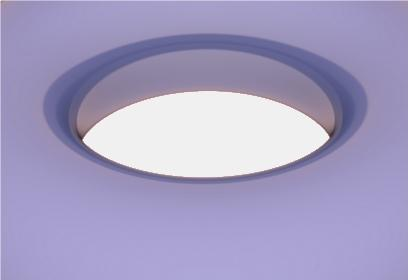
\includegraphics[scale=0.5]{./pictures/C1-torus-step1.jpg}
\end{center}\\
\end{tabular}

\begin{tabular}{m{2.5in} m{2in}}
\pause Ponieważ południki są znacznie krótsze niż równoleżniki, wprowadzamy zaburzenia wzdłuż równoleżników (falowanie).
&\begin{center}
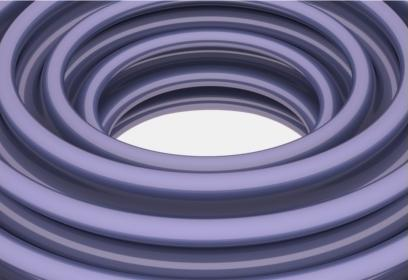
\includegraphics[scale=0.5]{./pictures/C1-torus-step2.jpg}
\end{center}\\
\end{tabular}
\end{frame}

\begin{frame}[plain]

\begin{tabular}{m{2.5in} m{2in}}
Teraz południki są faktycznie dłuższe, ale równoleżniki są (były) różnej długości, więc wprowadzamy drugi poziom falowania (mniejsza amplituda, a większa częstotliwość), aby wyrównać te różnice.
&\pause\begin{center}
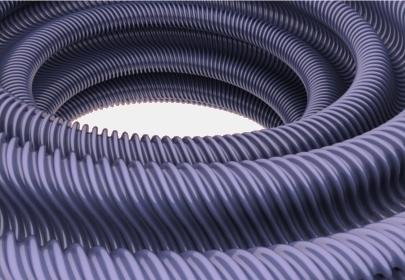
\includegraphics[scale=0.5]{./pictures/C1-torus-step3.jpg}
\end{center}\\
itd... 
\end{tabular}
\end{frame}
\newpage

\begin{frame}[plain]
\mode<presentation>{\hspace*{-0.9in}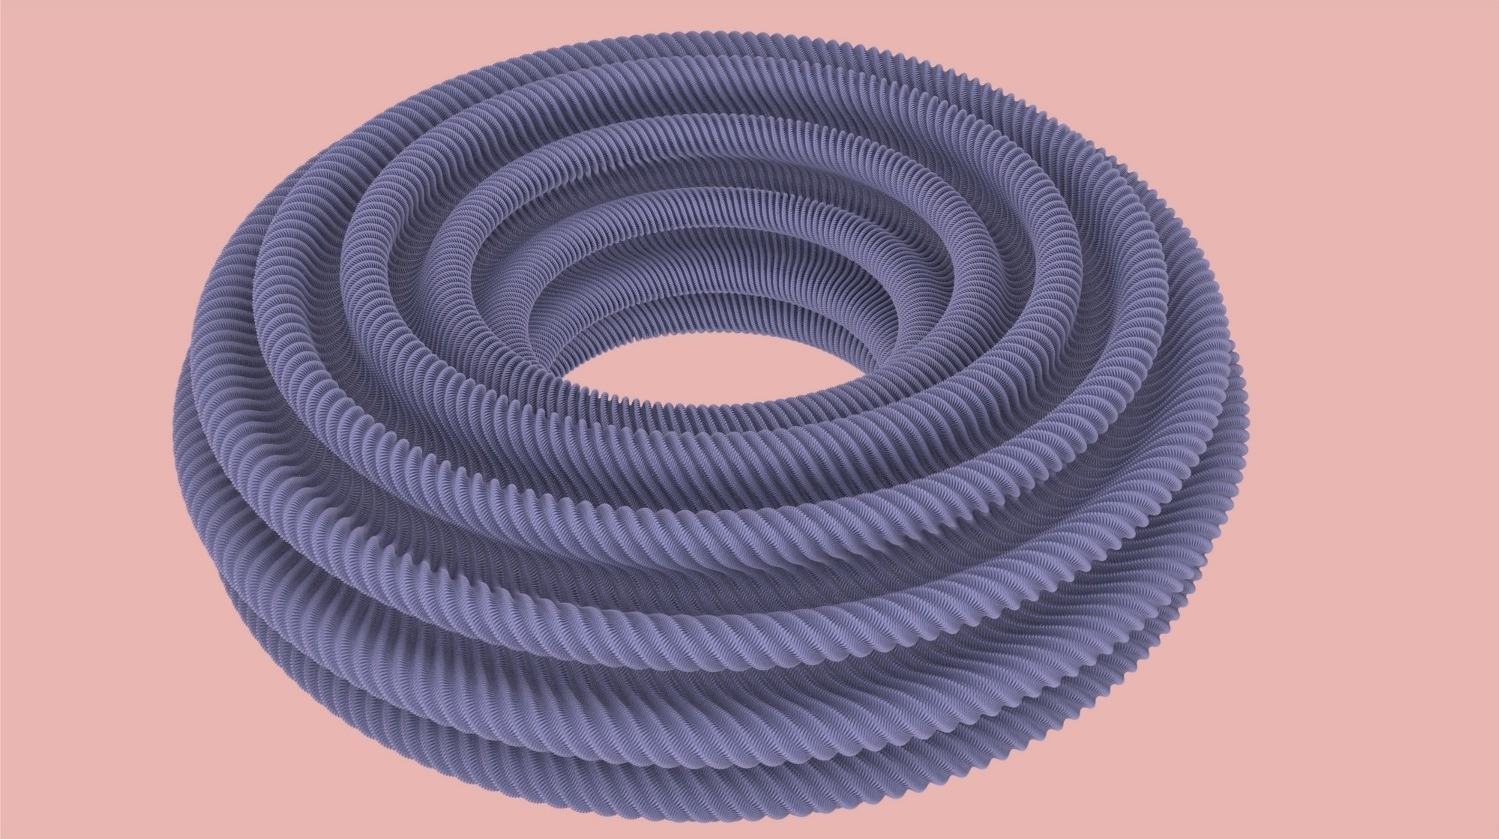
\includegraphics[scale=2]{./pictures/C1-flat-torus-1.png}}
\mode<article>{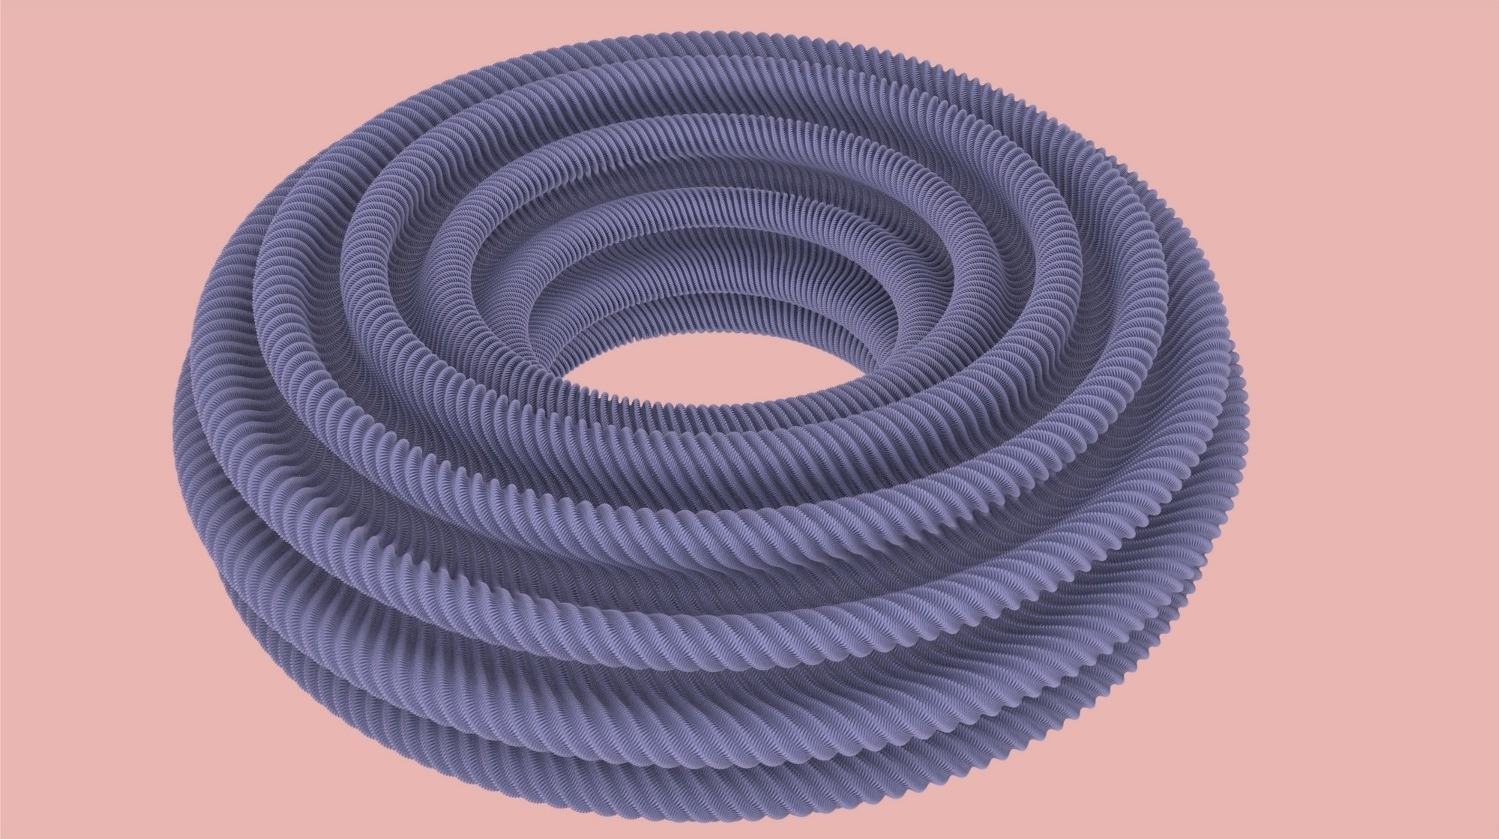
\includegraphics[keepaspectratio=true,width=\textwidth]{./pictures/C1-flat-torus-1.png}}
% \begin{center}
%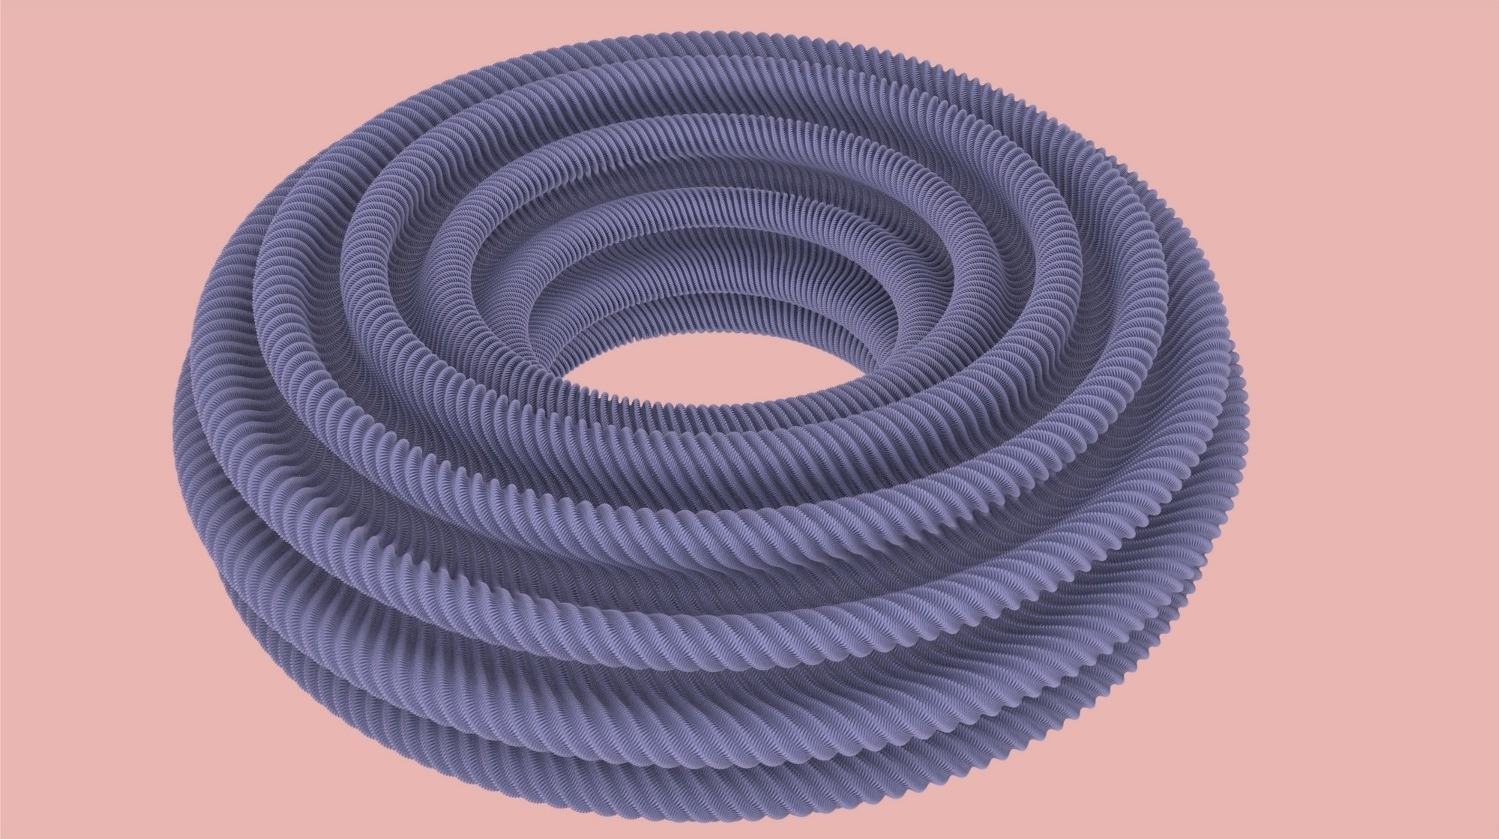
\includegraphics[keepaspectratio=true,width=1\paperwidth]{./pictures/C1-flat-torus-1.png}
% \end{center}
\end{frame}
\smallskip
%\newpage
\begin{frame}[plain]
\mode<presentation>{\hspace*{-0.9in}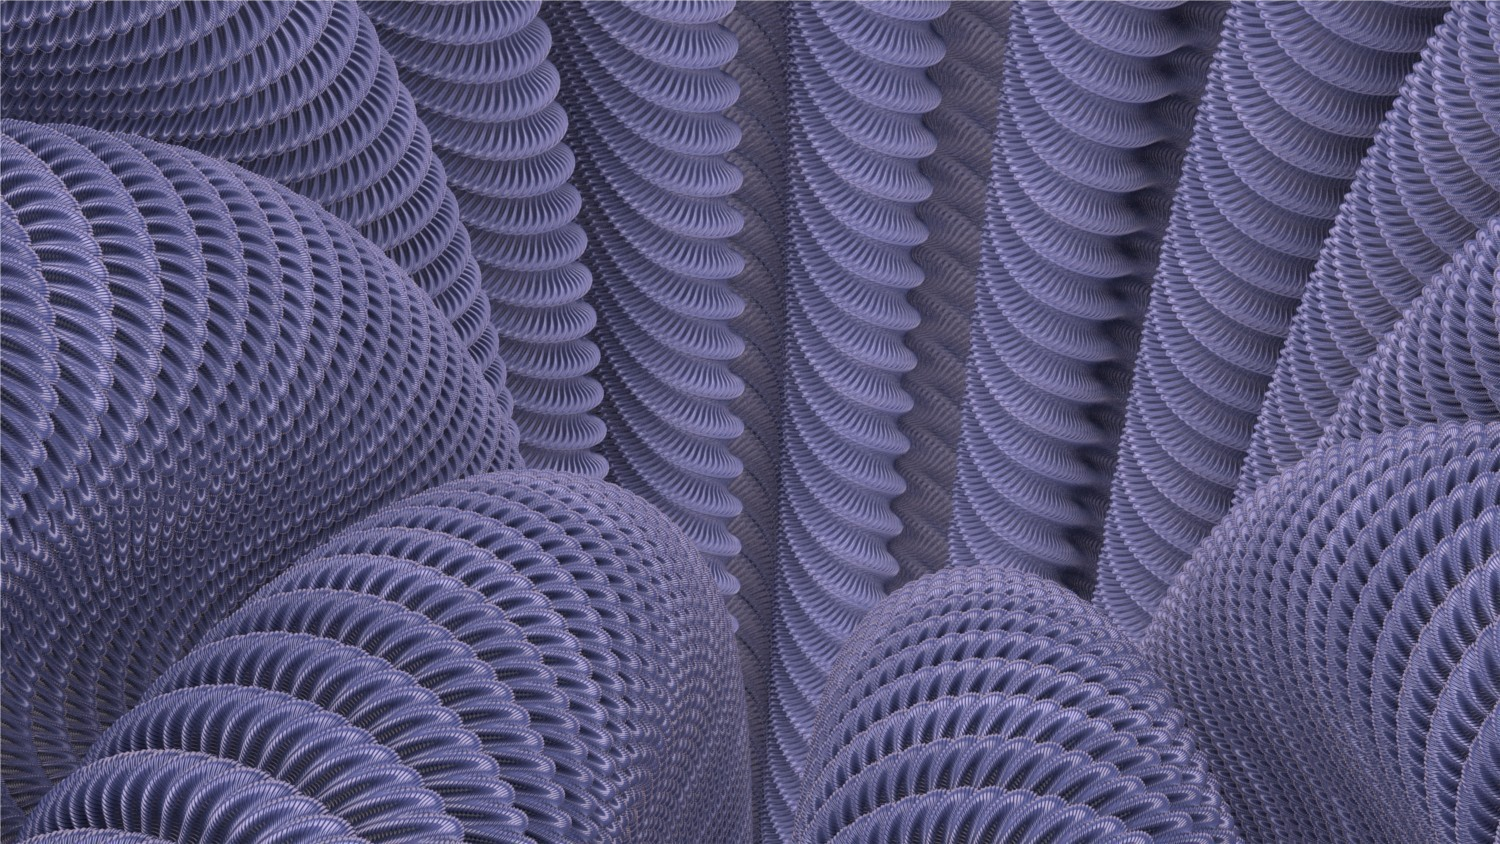
\includegraphics[scale=2]{./pictures/C1-flat-torus-2.png}}
\mode<article>{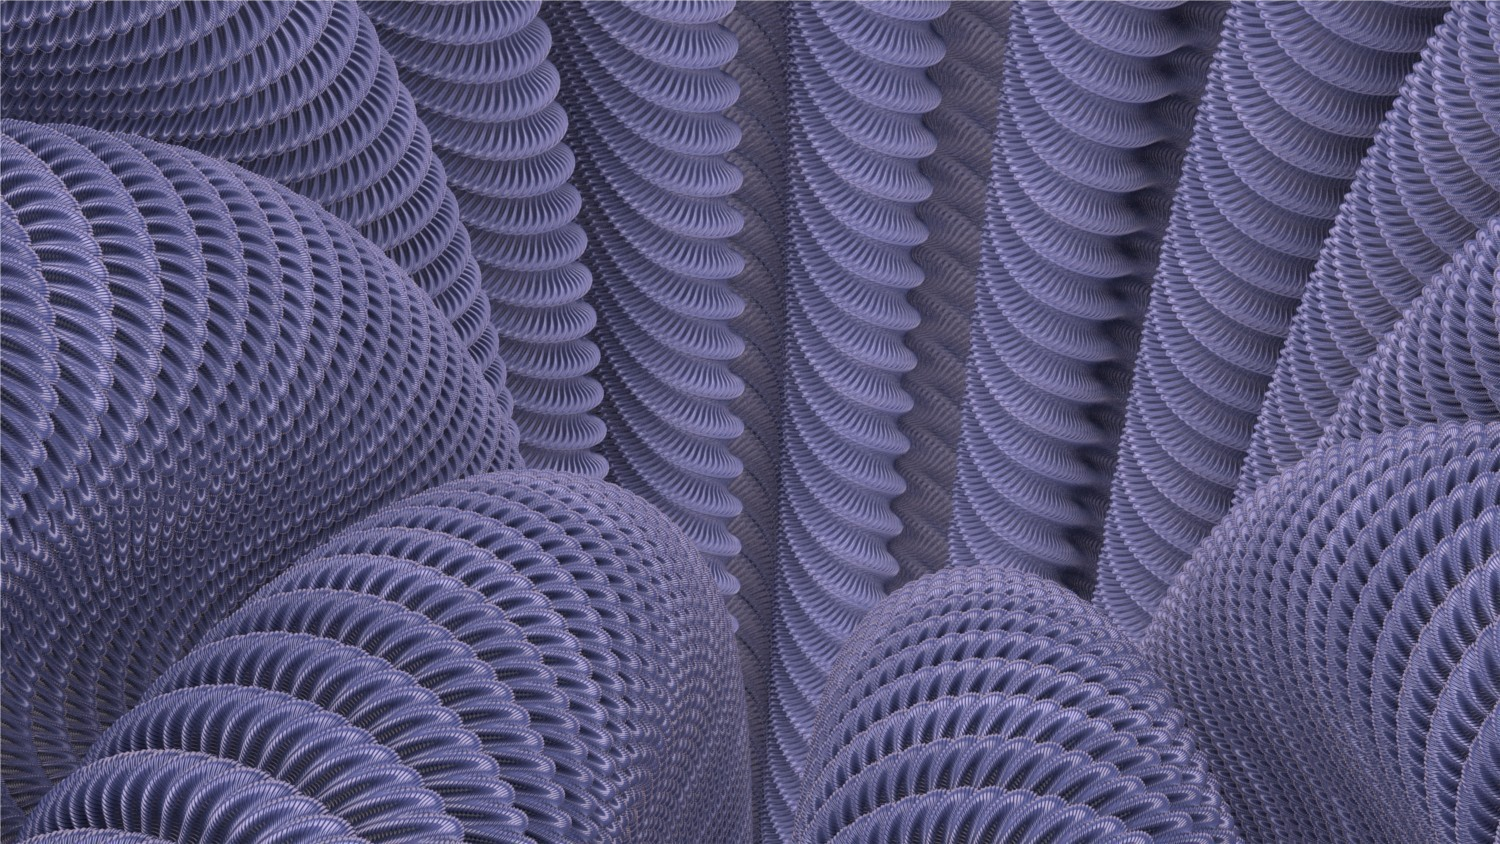
\includegraphics[keepaspectratio=true,width=\textwidth]{./pictures/C1-flat-torus-2.png}}
\end{frame}

%\newpage

\begin{frame}
\begin{itemize}
\item Chociaż wszystkie kroki można wykonać w klasie $C^2$, proces ten 
kontynuujemy w nieskończoność, więc ostateczne zanurzenie jako granica tych 
odwzorowań może być tylko klasy $C^1$.
\mode<article>{
\item Odwzorowanie klasy $C^1$ oznacza, że przestrzeń styczna jest w każdym 
punkcie zdefiniowana, lecz wektor normalny może zdradzać ,,dziwaczne" 
zachowanie (w przypadku tego zanurzenia -- fraktalne).
}
\pause \item Jednocześnie na rysunku poniżej widzimy, że południki i równoleżniki uzyskały tę samą długość.
\begin{center}
\mode<presentation>{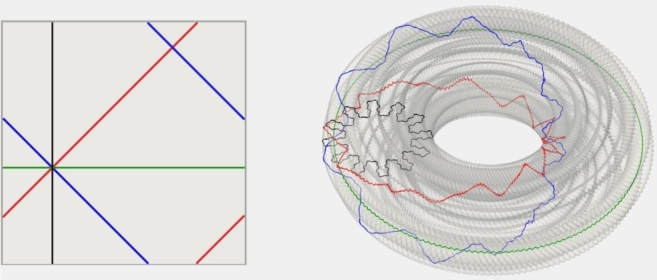
\includegraphics[scale=0.41]{./pictures/C1-flat-torus-equal.jpg}}
\mode<article>{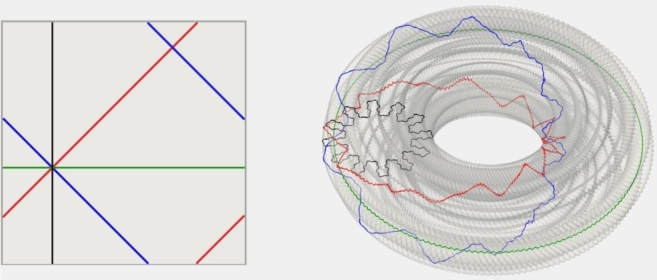
\includegraphics[keepaspectratio=true,width=\textwidth]{./pictures/C1-flat-torus-equal.jpg}}

\end{center}
\end{itemize}
\end{frame}

\begin{frame}[plain]
%\begin{center}
\mode<presentation>{\hspace*{-0.2in}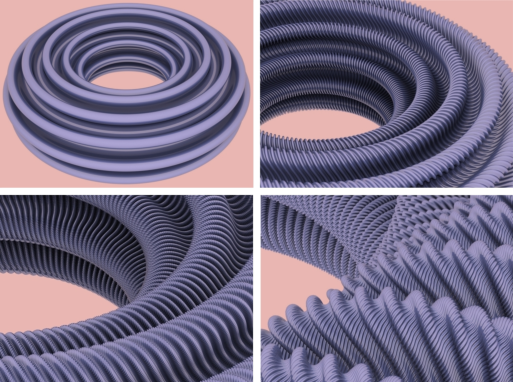
\includegraphics[scale=1.5]{./pictures/flat-torus-1.pdf}}
\mode<article>{\hspace*{0.4in}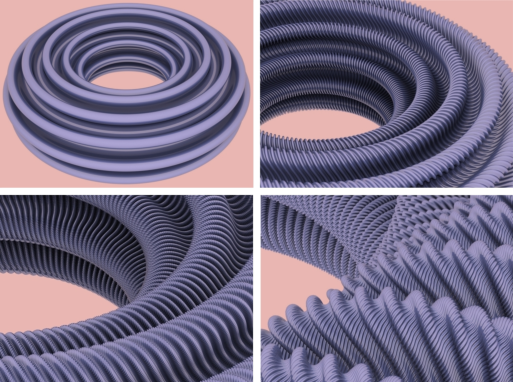
\includegraphics[keepaspectratio=true,width=\textwidth]{./pictures/flat-torus-1.pdf}}

%\end{center}
\end{frame}

% \footnotesize{Rysunki płaskiego zanurzenia torusa w $\R^3$ pochodzą z pracy:\\
% Borrelli, Vincent and Jabrane, Saïd and Lazarus, Francis and Thibert, Boris,
% \textit{Flat tori in three-dimensional space and convex integration}, Proceedings of the National Academy of Sciences, 2012}
\mode<all> 







\end{document}


